% -*- coding: utf-8 -*-
%!TEX program = xelatex
\documentclass[12pt]{ctexbook}
%\documentclass[draft,12pt]{ctexbook}   % draft草稿模式下,bookmark会被忽略 draft,
\def\allfiles{}
%\usepackage{xeCJK}
%\usepackage[14pt]{extsizes} %支持8,9,10,11,12,14,17,20pt

%===================文档页面设置====================
%---------------------印刷版尺寸--------------------
%\usepackage[a4paper,hmargin={2.3cm,1.7cm},vmargin=2.3cm,driver=xetex]{geometry}
%--------------------电子版------------------------
\usepackage[a4paper,margin=2cm,driver=xetex]{geometry}
%\usepackage[paperwidth=9.2cm, paperheight=12.4cm, width=9cm, height=12cm,top=0.2cm,
%            bottom=0.4cm,left=0.2cm,right=0.2cm,foot=0cm, nohead,nofoot,driver=xetex]{geometry}

%===================自定义颜色=====================
\usepackage{xcolor}
  \definecolor{mybackgroundcolor}{cmyk}{0.03,0.03,0.18,0}
  \definecolor{myblue}{rgb}{0,0.2,0.6}

%====================字体设置======================
%--------------------中文字体----------------------
%-----------------------xeCJK下设置中文字体------------------------------%
\setCJKfamilyfont{song}{SimSun}                             %宋体 song
\newcommand{\song}{\CJKfamily{song}}                        % 宋体   (Windows自带simsun.ttf)
\setCJKfamilyfont{xs}{NSimSun}                              %新宋体 xs
\newcommand{\xs}{\CJKfamily{xs}}
\setCJKfamilyfont{fs}{FangSong_GB2312}                      %仿宋2312 fs
\newcommand{\fs}{\CJKfamily{fs}}                            %仿宋体 (Windows自带simfs.ttf)
\setCJKfamilyfont{kai}{KaiTi_GB2312}                        %楷体2312  kai
\newcommand{\kai}{\CJKfamily{kai}}
\setCJKfamilyfont{yh}{Microsoft YaHei}                    %微软雅黑 yh
\newcommand{\yh}{\CJKfamily{yh}}
\setCJKfamilyfont{hei}{SimHei}                                    %黑体  hei
\newcommand{\hei}{\CJKfamily{hei}}                          % 黑体   (Windows自带simhei.ttf)
\setCJKfamilyfont{msunicode}{Arial Unicode MS}            %Arial Unicode MS: msunicode
\newcommand{\msunicode}{\CJKfamily{msunicode}}
\setCJKfamilyfont{li}{LiSu}                                            %隶书  li
\newcommand{\li}{\CJKfamily{li}}
\setCJKfamilyfont{yy}{YouYuan}                             %幼圆  yy
\newcommand{\yy}{\CJKfamily{yy}}
\setCJKfamilyfont{xm}{MingLiU}                                        %细明体  xm
\newcommand{\xm}{\CJKfamily{xm}}
\setCJKfamilyfont{xxm}{PMingLiU}                             %新细明体  xxm
\newcommand{\xxm}{\CJKfamily{xxm}}

\setCJKfamilyfont{hwsong}{STSong}                            %华文宋体  hwsong
\newcommand{\hwsong}{\CJKfamily{hwsong}}
\setCJKfamilyfont{hwzs}{STZhongsong}                        %华文中宋  hwzs
\newcommand{\hwzs}{\CJKfamily{hwzs}}
\setCJKfamilyfont{hwfs}{STFangsong}                            %华文仿宋  hwfs
\newcommand{\hwfs}{\CJKfamily{hwfs}}
\setCJKfamilyfont{hwxh}{STXihei}                                %华文细黑  hwxh
\newcommand{\hwxh}{\CJKfamily{hwxh}}
\setCJKfamilyfont{hwl}{STLiti}                                        %华文隶书  hwl
\newcommand{\hwl}{\CJKfamily{hwl}}
\setCJKfamilyfont{hwxw}{STXinwei}                                %华文新魏  hwxw
\newcommand{\hwxw}{\CJKfamily{hwxw}}
\setCJKfamilyfont{hwk}{STKaiti}                                    %华文楷体  hwk
\newcommand{\hwk}{\CJKfamily{hwk}}
\setCJKfamilyfont{hwxk}{STXingkai}                            %华文行楷  hwxk
\newcommand{\hwxk}{\CJKfamily{hwxk}}
\setCJKfamilyfont{hwcy}{STCaiyun}                                 %华文彩云 hwcy
\newcommand{\hwcy}{\CJKfamily{hwcy}}
\setCJKfamilyfont{hwhp}{STHupo}                                 %华文琥珀   hwhp
\newcommand{\hwhp}{\CJKfamily{hwhp}}

\setCJKfamilyfont{fzsong}{Simsun (Founder Extended)}     %方正宋体超大字符集   fzsong
\newcommand{\fzsong}{\CJKfamily{fzsong}}
\setCJKfamilyfont{fzyao}{FZYaoTi}                                    %方正姚体  fzy
\newcommand{\fzyao}{\CJKfamily{fzyao}}
\setCJKfamilyfont{fzshu}{FZShuTi}                                    %方正舒体 fzshu
\newcommand{\fzshu}{\CJKfamily{fzshu}}

\setCJKfamilyfont{asong}{Adobe Song Std}                        %Adobe 宋体  asong
\newcommand{\asong}{\CJKfamily{asong}}
\setCJKfamilyfont{ahei}{Adobe Heiti Std}                            %Adobe 黑体  ahei
\newcommand{\ahei}{\CJKfamily{ahei}}
\setCJKfamilyfont{akai}{Adobe Kaiti Std}                            %Adobe 楷体  akai
\newcommand{\akai}{\CJKfamily{akai}}

%------------------------------设置字体大小------------------------%
\newcommand{\chuhao}{\fontsize{42pt}{\baselineskip}\selectfont}     %初号
\newcommand{\xiaochuhao}{\fontsize{36pt}{\baselineskip}\selectfont} %小初号
\newcommand{\yihao}{\fontsize{28pt}{\baselineskip}\selectfont}      %一号
\newcommand{\xiaoyihao}{\fontsize{24pt}{\baselineskip}\selectfont}
\newcommand{\erhao}{\fontsize{21pt}{\baselineskip}\selectfont}      %二号
\newcommand{\xiaoerhao}{\fontsize{18pt}{\baselineskip}\selectfont}  %小二号
\newcommand{\sanhao}{\fontsize{15.75pt}{\baselineskip}\selectfont}  %三号
\newcommand{\sihao}{\fontsize{14pt}{\baselineskip}\selectfont}%     四号
\newcommand{\xiaosihao}{\fontsize{12pt}{\baselineskip}\selectfont}  %小四号
\newcommand{\wuhao}{\fontsize{10.5pt}{\baselineskip}\selectfont}    %五号
\newcommand{\xiaowuhao}{\fontsize{9pt}{\baselineskip}\selectfont}   %小五号
\newcommand{\liuhao}{\fontsize{7.875pt}{\baselineskip}\selectfont}  %六号
\newcommand{\qihao}{\fontsize{5.25pt}{\baselineskip}\selectfont}    %七号   %中文字体及字号设置
\xeCJKDeclareSubCJKBlock{SIP}{
  "20000 -> "2A6DF,   % CJK Unified Ideographs Extension B
  "2A700 -> "2B73F,   % CJK Unified Ideographs Extension C
  "2B740 -> "2B81F    % CJK Unified Ideographs Extension D
}
%\setCJKmainfont[SIP={[AutoFakeBold=1.8,Color=red]Sun-ExtB},BoldFont=黑体]{宋体}    % 衬线字体 缺省中文字体

\setCJKmainfont{simsun.ttc}[
  Path=fonts/,
  SIP={[Path=fonts/,AutoFakeBold=1.8,Color=red]simsunb.ttf},
  BoldFont=simhei.ttf
]

%SimSun-ExtB
%Sun-ExtB
%AutoFakeBold:自动伪粗,即正文使用\bfseries时生僻字使用伪粗体;
%FakeBold:强制伪粗,即正文中生僻字均使用伪粗体
%\setCJKmainfont[BoldFont=STHeiti,ItalicFont=STKaiti]{STSong}
%\setCJKsansfont{微软雅黑}黑体
%\setCJKsansfont[BoldFont=STHeiti]{STXihei} %serif是有衬线字体sans serif 无衬线字体
%\setCJKmonofont{STFangsong}    %中文等宽字体

%--------------------英文字体----------------------
\setmainfont{simsun.ttc}[
  Path=fonts/,
  BoldFont=simhei.ttf
]
%\setmainfont[BoldFont=黑体]{宋体}  %缺省英文字体
%\setsansfont
%\setmonofont

%===================目录分栏设置====================
\usepackage[toc,lof,lot]{multitoc}    % 目录(含目录、表格目录、插图目录)分栏设置
  %\renewcommand*{\multicolumntoc}{3} % toc分栏数设置,默认为两栏(\multicolumnlof,\multicolumnlot)
  %\setlength{\columnsep}{1.5cm}      % 调整分栏间距
  \setlength{\columnseprule}{0.2pt}   % 调整分栏竖线的宽度

%==================章节格式设置====================
\setcounter{secnumdepth}{3} % 章节等编号深度 3:子子节\subsubsection
\setcounter{tocdepth}{2}    % 目录显示等度 2:子节

\xeCJKsetup{%
  CJKecglue=\hspace{0.15em},      % 调整中英(含数字)间的字间距
  %CJKmath=true,                  % 在数学环境中直接输出汉字(不需要\text{})
  AllowBreakBetweenPuncts=true,   % 允许标点中间断行,减少文字行溢出
}

\ctexset{%
  part={
    name={,篇},
    number=\SZX{part},
    format={\chuhao\bfseries\centering},
    nameformat={},titleformat={}
  },
  section={
    number={\chinese{section}},
    name={第,节}
  },
  subsection={
    number={\chinese{subsection}、},
    aftername={\hspace{-0.01em}}
  },
  subsubsection={
    number={(\chinese{subsubsection})},
    aftername={\hspace {-0.01em}},
    beforeskip={1.3ex minus .8ex},
    afterskip={1ex minus .6ex},
    indent={\parindent}
  },
  paragraph={
    beforeskip=.1\baselineskip,
    indent={\parindent}
  }
}

\newcommand*\SZX[1]{%
  \ifcase\value{#1}%
    \or 上%
    \or 中%
    \or 下%
  \fi
}

%====================页眉设置======================
\usepackage{titleps}%或者\usepackage{titlesec},titlesec包含titleps
\newpagestyle{special}[\small\sffamily]{
  %\setheadrule{.1pt}
  \headrule
  \sethead[\usepage][][\chaptertitle]
  {\chaptertitle}{}{\usepage}
}

\newpagestyle{main}[\small\sffamily]{
  \headrule
  %\sethead[\usepage][][第\thechapter 章\quad\chaptertitle]
%  {\thesection\quad\sectiontitle}{}{\usepage}}
  \sethead[\usepage][][第\chinese{chapter}章\quad\chaptertitle]
  {第\chinese{section}节\quad\sectiontitle}{}{\usepage}
}

\newpagestyle{main2}[\small\sffamily]{
  \headrule
  \sethead[\usepage][][第\chinese{chapter}章\quad\chaptertitle]
  {第\chinese{section}節\quad\sectiontitle}{}{\usepage}
}

%================ PDF 书签设置=====================
\usepackage{bookmark}[
  depth=2,        % 书签深度 2:子节
  open,           % 默认展开书签
  openlevel=2,    % 展开书签深度 2:子节
  numbered,       % 显示编号
  atend,
]
  % 相比hyperref,bookmark宏包大多数时候只需要编译一次,
  % 而且书签的颜色和字体也可以定制。
  % 比hyperref 更专业 (自动加载hyperref)

%\bookmarksetup{italic,bold,color=blue} % 书签字体斜体/粗体/颜色设置

%------------重置每篇章计数器,必须在hyperref/bookmark之后------------
\makeatletter
  \@addtoreset{chapter}{part}
\makeatother

%------------hyperref 超链接设置------------------------
\hypersetup{%
  pdfencoding=auto,   % 解决新版ctex,引起hyperref UTF-16预警
  colorlinks=true,    % 注释掉此项则交叉引用为彩色边框true/false
  pdfborder=001,      % 注释掉此项则交叉引用为彩色边框
  citecolor=teal,
  linkcolor=myblue,
  urlcolor=black,
  %psdextra,          % 配合使用bookmark宏包,可以直接在pdf 书签中显示数学公式
}

%------------PDF 属性设置------------------------------
\hypersetup{%
  pdfkeywords={黄帝内经,内经,内经讲义,21世纪课程教材},    % 关键词
  %pdfsubject={latex},        % 主题
  pdfauthor={主编:王洪图},   % 作者
  pdftitle={内经讲义},        % 标题
  %pdfcreator={texlive2011}   % pdf创建器
}

%------------PDF 加密----------------------------------
%仅适用于xelatex引擎 基于xdvipdfmx
%\special{pdf:encrypt ownerpw (abc) userpw (xyz) length 128 perm 2052}

%仅适用于pdflatex引擎
%\usepackage[owner=Donald,user=Knuth,print=false]{pdfcrypt}

%其他可使用第三方工具 如:pdftk
%pdftk inputfile.pdf output outputfile.pdf encrypt_128bit owner_pw yourownerpw user_pw youruserpw

%=============自定义环境、列表及列表设置================
% 标题
\def\biaoti#1{\vspace{1.7ex plus 3ex minus .2ex}{\bfseries #1}}%\noindent\hei
% 小标题
\def\xiaobt#1{{\bfseries #1}}
% 小结
\def\xiaojie {\vspace{1.8ex plus .3ex minus .3ex}\centerline{\large\bfseries 小\ \ 结}\vspace{.1\baselineskip}}
% 作者
\def\zuozhe#1{\rightline{\bfseries #1}}

\newcounter{yuanwen}    % 新计数器 yuanwen
\newcounter{jiaozhu}    % 新计数器 jiaozhu

\newenvironment{yuanwen}[2][【原文】]{%
  %\biaoti{#1}\par
  \stepcounter{yuanwen}   % 计数器 yuanwen+1
  \bfseries #2}
  {}

\usepackage{enumitem}
\newenvironment{jiaozhu}[1][【校注】]{%
  %\biaoti{#1}\par
  \stepcounter{jiaozhu}   % 计数器 jiaozhu+1
  \begin{enumerate}[%
    label=\mylabel{\arabic*}{\circledctr*},before=\small,fullwidth,%
    itemindent=\parindent,listparindent=\parindent,%labelsep=-1pt,%labelwidth=0em,
    itemsep=0pt,topsep=0pt,partopsep=0pt,parsep=0pt
  ]}
  {\end{enumerate}}

%===================注解与原文相互跳转====================
%----------------第1部分 设置相互跳转锚点-----------------
\makeatletter
  \protected\def\mylabel#1#2{% 注解-->原文
    \hyperlink{back:\theyuanwen:#1}{\Hy@raisedlink{\hypertarget{\thejiaozhu:#1}{}}#2}}

  \protected\def\myref#1#2{% 原文-->注解
    \hyperlink{\theyuanwen:#1}{\Hy@raisedlink{\hypertarget{back:\theyuanwen:#1}{}}#2}}
  %此处\theyuanwen:#1实际指thejiaozhu:#1,只是\thejiaozhu计数器还没更新,故使用\theyuanwen计数器代替
\makeatother

\protected\def\myjzref#1{% 脚注中的引用(引用到原文)
  \hyperlink{\theyuanwen:#1}{\circlednum{#1}}}

\def\sb#1{\myref{#1}{\textsuperscript{\circlednum{#1}}}}    % 带圈数字上标

%----------------第2部分 调整锚点垂直距离-----------------
\def\HyperRaiseLinkDefault{.8\baselineskip} %调整锚点垂直距离
%\let\oldhypertarget\hypertarget
%\makeatletter
%  \def\hypertarget#1#2{\Hy@raisedlink{\oldhypertarget{#1}{#2}}}
%\makeatother

%====================带圈数字列表标头====================
\newfontfamily\circledfont[Path = fonts/]{meiryo.ttc}  % 日文字体,明瞭体
%\newfontfamily\circledfont{Meiryo}  % 日文字体,明瞭体

\protected\def\circlednum#1{{\makexeCJKinactive\circledfont\textcircled{#1}}}

\newcommand*\circledctr[1]{%
  \expandafter\circlednum\expandafter{\number\value{#1}}}
\AddEnumerateCounter*\circledctr\circlednum{1}

% 参考自:http://bbs.ctex.org/forum.php?mod=redirect&goto=findpost&ptid=78709&pid=460496&fromuid=40353

%======================插图/tikz图========================
\usepackage{graphicx,subcaption,wrapfig}    % 图,subcaption含子图功能代替subfig,图文混排
  \graphicspath{{img/}}                     % 设置图片文件路径

\def\pgfsysdriver{pgfsys-xetex.def}         % 设置tikz的驱动引擎
\usepackage{tikz}
  \usetikzlibrary{calc,decorations.text,arrows,positioning}

%---------设置tikz图片默认格式(字号、行间距、单元格高度)-------
\let\oldtikzpicture\tikzpicture
\renewcommand{\tikzpicture}{%
  \small
  \renewcommand{\baselinestretch}{0.2}
  \linespread{0.2}
  \oldtikzpicture
}

%=========================表格相关===============================
\usepackage{%
  multirow,                   % 单元格纵向合并
  array,makecell,longtable,   % 表格功能加强,tabu的依赖
  tabu-last-fix,              % "强大的表格工具" 本地修复版
  diagbox,                    % 表头斜线
  threeparttable,             % 表格内脚注(需打补丁支持tabu,longtabu)
}

%----------给threeparttable打补丁用于tabu,longtabu--------------
%解决方案来自:http://bbs.ctex.org/forum.php?mod=redirect&goto=findpost&ptid=80318&pid=467217&fromuid=40353
\usepackage{xpatch}

\makeatletter
  \chardef\TPT@@@asteriskcatcode=\catcode`*
  \catcode`*=11
  \xpatchcmd{\threeparttable}
    {\TPT@hookin{tabular}}
    {\TPT@hookin{tabular}\TPT@hookin{tabu}}
    {}{}
  \catcode`*=\TPT@@@asteriskcatcode
\makeatother

%------------设置表格默认格式(字号、行间距、单元格高度)------------
\let\oldtabular\tabular
\renewcommand{\tabular}{%
  \renewcommand\baselinestretch{0.9}\small    % 设置行间距和字号
  \renewcommand\arraystretch{1.5}             % 调整单元格高度
  %\renewcommand\multirowsetup{\centering}
  \oldtabular
}
%设置行间距,且必须放在字号设置前 否则无效
%或者使用\fontsize{<size>}{<baseline>}\selectfont 同时设置字号和行间距

\let\oldtabu\tabu
\renewcommand{\tabu}{%
  \renewcommand\baselinestretch{0.9}\small    % 设置行间距和字号
  \renewcommand\arraystretch{1.8}             % 调整单元格高度
  %\renewcommand\multirowsetup{\centering}
  \oldtabu
}

%------------模仿booktabs宏包的三线宽度设置---------------
\def\toprule   {\Xhline{.08em}}
\def\midrule   {\Xhline{.05em}}
\def\bottomrule{\Xhline{.08em}}
%-------------------------------------
%\setlength{\arrayrulewidth}{2pt} 设定表格中所有边框的线宽为同样的值
%\Xhline{} \Xcline{}分别设定表格中水平线的宽度 makecell包提供

%表格中垂直线的宽度可以通过在表格导言区(preamble),利用命令 !{\vrule width1.2pt} 替换 | 即可

%=================图表设置===============================
%---------------图表标号设置-----------------------------
\renewcommand\thefigure{\arabic{section}-\arabic{figure}}
\renewcommand\thetable {\arabic{section}-\arabic{table}}

\usepackage{caption}
  \captionsetup{font=small,}
  \captionsetup[table] {labelfont=bf,textfont=bf,belowskip=3pt,aboveskip=0pt} %仅表格 top
  \captionsetup[figure]{belowskip=0pt,aboveskip=3pt}  %仅图片 below

%\setlength{\abovecaptionskip}{3pt}
%\setlength{\belowcaptionskip}{3pt} %图、表题目上下的间距
\setlength{\intextsep}   {5pt}  %浮动体和正文间的距离
\setlength{\textfloatsep}{5pt}

%====================全文水印==========================
%解决方案来自:
%http://bbs.ctex.org/forum.php?mod=redirect&goto=findpost&ptid=79190&pid=462496&fromuid=40353
%https://zhuanlan.zhihu.com/p/19734756?columnSlug=LaTeX
\usepackage{eso-pic}

%eso-pic中\AtPageCenter有点水平偏右
\renewcommand\AtPageCenter[1]{\parbox[b][\paperheight]{\paperwidth}{\vfill\centering#1\vfill}}

\newcommand{\watermark}[3]{%
  \AddToShipoutPictureBG{%
    \AtPageCenter{%
      \tikz\node[%
        overlay,
        text=red!50,
        %font=\sffamily\bfseries,
        rotate=#1,
        scale=#2
      ]{#3};
    }
  }
}

\newcommand{\watermarkoff}{\ClearShipoutPictureBG}

\watermark{45}{15}{草\ 稿}    %启用全文水印

%=============花括号分支结构图=========================
\usepackage{schemata}

\xpatchcmd{\schema}
  {1.44265ex}{-1ex}
  {}{}

\newcommand\SC[2] {\schema{\schemabox{#1}}{\schemabox{#2}}}
\newcommand\SCh[4]{\Schema{#1}{#2}{\schemabox{#3}}{\schemabox{#4}}}

%=======================================================

\begin{document}
%\pagecolor{mybackgroundcolor}  % 启用全文背景色
\watermarkoff                   % 关闭全文水印
\clearpage

%------------------封面页------------------
\pdfbookmark[-2]{《内经讲义》}{title} % 将文章标题添加到pdf书签中,且最高层
% -*- coding: utf-8 -*-
%!TEX program = xelatex
\ifx \allfiles \undefined
\documentclass[12pt]{ctexbook}%draft,
%\usepackage{xeCJK}
%\usepackage[14pt]{extsizes} %支持8,9,10,11,12,14,17,20pt

%===================文档页面设置====================
%---------------------印刷版尺寸--------------------
%\usepackage[a4paper,hmargin={2.3cm,1.7cm},vmargin=2.3cm,driver=xetex]{geometry}
%--------------------电子版------------------------
\usepackage[a4paper,margin=2cm,driver=xetex]{geometry}
%\usepackage[paperwidth=9.2cm, paperheight=12.4cm, width=9cm, height=12cm,top=0.2cm,
%            bottom=0.4cm,left=0.2cm,right=0.2cm,foot=0cm, nohead,nofoot,driver=xetex]{geometry}

%===================自定义颜色=====================
\usepackage{xcolor}
  \definecolor{mybackgroundcolor}{cmyk}{0.03,0.03,0.18,0}
  \definecolor{myblue}{rgb}{0,0.2,0.6}

%====================字体设置======================
%--------------------中文字体----------------------
%-----------------------xeCJK下设置中文字体------------------------------%
\setCJKfamilyfont{song}{SimSun}                             %宋体 song
\newcommand{\song}{\CJKfamily{song}}                        % 宋体   (Windows自带simsun.ttf)
\setCJKfamilyfont{xs}{NSimSun}                              %新宋体 xs
\newcommand{\xs}{\CJKfamily{xs}}
\setCJKfamilyfont{fs}{FangSong_GB2312}                      %仿宋2312 fs
\newcommand{\fs}{\CJKfamily{fs}}                            %仿宋体 (Windows自带simfs.ttf)
\setCJKfamilyfont{kai}{KaiTi_GB2312}                        %楷体2312  kai
\newcommand{\kai}{\CJKfamily{kai}}
\setCJKfamilyfont{yh}{Microsoft YaHei}                    %微软雅黑 yh
\newcommand{\yh}{\CJKfamily{yh}}
\setCJKfamilyfont{hei}{SimHei}                                    %黑体  hei
\newcommand{\hei}{\CJKfamily{hei}}                          % 黑体   (Windows自带simhei.ttf)
\setCJKfamilyfont{msunicode}{Arial Unicode MS}            %Arial Unicode MS: msunicode
\newcommand{\msunicode}{\CJKfamily{msunicode}}
\setCJKfamilyfont{li}{LiSu}                                            %隶书  li
\newcommand{\li}{\CJKfamily{li}}
\setCJKfamilyfont{yy}{YouYuan}                             %幼圆  yy
\newcommand{\yy}{\CJKfamily{yy}}
\setCJKfamilyfont{xm}{MingLiU}                                        %细明体  xm
\newcommand{\xm}{\CJKfamily{xm}}
\setCJKfamilyfont{xxm}{PMingLiU}                             %新细明体  xxm
\newcommand{\xxm}{\CJKfamily{xxm}}

\setCJKfamilyfont{hwsong}{STSong}                            %华文宋体  hwsong
\newcommand{\hwsong}{\CJKfamily{hwsong}}
\setCJKfamilyfont{hwzs}{STZhongsong}                        %华文中宋  hwzs
\newcommand{\hwzs}{\CJKfamily{hwzs}}
\setCJKfamilyfont{hwfs}{STFangsong}                            %华文仿宋  hwfs
\newcommand{\hwfs}{\CJKfamily{hwfs}}
\setCJKfamilyfont{hwxh}{STXihei}                                %华文细黑  hwxh
\newcommand{\hwxh}{\CJKfamily{hwxh}}
\setCJKfamilyfont{hwl}{STLiti}                                        %华文隶书  hwl
\newcommand{\hwl}{\CJKfamily{hwl}}
\setCJKfamilyfont{hwxw}{STXinwei}                                %华文新魏  hwxw
\newcommand{\hwxw}{\CJKfamily{hwxw}}
\setCJKfamilyfont{hwk}{STKaiti}                                    %华文楷体  hwk
\newcommand{\hwk}{\CJKfamily{hwk}}
\setCJKfamilyfont{hwxk}{STXingkai}                            %华文行楷  hwxk
\newcommand{\hwxk}{\CJKfamily{hwxk}}
\setCJKfamilyfont{hwcy}{STCaiyun}                                 %华文彩云 hwcy
\newcommand{\hwcy}{\CJKfamily{hwcy}}
\setCJKfamilyfont{hwhp}{STHupo}                                 %华文琥珀   hwhp
\newcommand{\hwhp}{\CJKfamily{hwhp}}

\setCJKfamilyfont{fzsong}{Simsun (Founder Extended)}     %方正宋体超大字符集   fzsong
\newcommand{\fzsong}{\CJKfamily{fzsong}}
\setCJKfamilyfont{fzyao}{FZYaoTi}                                    %方正姚体  fzy
\newcommand{\fzyao}{\CJKfamily{fzyao}}
\setCJKfamilyfont{fzshu}{FZShuTi}                                    %方正舒体 fzshu
\newcommand{\fzshu}{\CJKfamily{fzshu}}

\setCJKfamilyfont{asong}{Adobe Song Std}                        %Adobe 宋体  asong
\newcommand{\asong}{\CJKfamily{asong}}
\setCJKfamilyfont{ahei}{Adobe Heiti Std}                            %Adobe 黑体  ahei
\newcommand{\ahei}{\CJKfamily{ahei}}
\setCJKfamilyfont{akai}{Adobe Kaiti Std}                            %Adobe 楷体  akai
\newcommand{\akai}{\CJKfamily{akai}}

%------------------------------设置字体大小------------------------%
\newcommand{\chuhao}{\fontsize{42pt}{\baselineskip}\selectfont}     %初号
\newcommand{\xiaochuhao}{\fontsize{36pt}{\baselineskip}\selectfont} %小初号
\newcommand{\yihao}{\fontsize{28pt}{\baselineskip}\selectfont}      %一号
\newcommand{\xiaoyihao}{\fontsize{24pt}{\baselineskip}\selectfont}
\newcommand{\erhao}{\fontsize{21pt}{\baselineskip}\selectfont}      %二号
\newcommand{\xiaoerhao}{\fontsize{18pt}{\baselineskip}\selectfont}  %小二号
\newcommand{\sanhao}{\fontsize{15.75pt}{\baselineskip}\selectfont}  %三号
\newcommand{\sihao}{\fontsize{14pt}{\baselineskip}\selectfont}%     四号
\newcommand{\xiaosihao}{\fontsize{12pt}{\baselineskip}\selectfont}  %小四号
\newcommand{\wuhao}{\fontsize{10.5pt}{\baselineskip}\selectfont}    %五号
\newcommand{\xiaowuhao}{\fontsize{9pt}{\baselineskip}\selectfont}   %小五号
\newcommand{\liuhao}{\fontsize{7.875pt}{\baselineskip}\selectfont}  %六号
\newcommand{\qihao}{\fontsize{5.25pt}{\baselineskip}\selectfont}    %七号   %中文字体及字号设置
\xeCJKDeclareSubCJKBlock{SIP}{
  "20000 -> "2A6DF,   % CJK Unified Ideographs Extension B
  "2A700 -> "2B73F,   % CJK Unified Ideographs Extension C
  "2B740 -> "2B81F    % CJK Unified Ideographs Extension D
}
%\setCJKmainfont[SIP={[AutoFakeBold=1.8,Color=red]Sun-ExtB},BoldFont=黑体]{宋体}    % 衬线字体 缺省中文字体

\setCJKmainfont{simsun.ttc}[
  Path=fonts/,
  SIP={[Path=fonts/,AutoFakeBold=1.8,Color=red]simsunb.ttf},
  BoldFont=simhei.ttf
]

%SimSun-ExtB
%Sun-ExtB
%AutoFakeBold:自动伪粗,即正文使用\bfseries时生僻字使用伪粗体;
%FakeBold:强制伪粗,即正文中生僻字均使用伪粗体
%\setCJKmainfont[BoldFont=STHeiti,ItalicFont=STKaiti]{STSong}
%\setCJKsansfont{微软雅黑}黑体
%\setCJKsansfont[BoldFont=STHeiti]{STXihei} %serif是有衬线字体sans serif 无衬线字体
%\setCJKmonofont{STFangsong}    %中文等宽字体

%--------------------英文字体----------------------
\setmainfont{simsun.ttc}[
  Path=fonts/,
  BoldFont=simhei.ttf
]
%\setmainfont[BoldFont=黑体]{宋体}  %缺省英文字体
%\setsansfont
%\setmonofont

%===================目录分栏设置====================
\usepackage[toc,lof,lot]{multitoc}    % 目录(含目录、表格目录、插图目录)分栏设置
  %\renewcommand*{\multicolumntoc}{3} % toc分栏数设置,默认为两栏(\multicolumnlof,\multicolumnlot)
  %\setlength{\columnsep}{1.5cm}      % 调整分栏间距
  \setlength{\columnseprule}{0.2pt}   % 调整分栏竖线的宽度

%==================章节格式设置====================
\setcounter{secnumdepth}{3} % 章节等编号深度 3:子子节\subsubsection
\setcounter{tocdepth}{2}    % 目录显示等度 2:子节

\xeCJKsetup{%
  CJKecglue=\hspace{0.15em},      % 调整中英(含数字)间的字间距
  %CJKmath=true,                  % 在数学环境中直接输出汉字(不需要\text{})
  AllowBreakBetweenPuncts=true,   % 允许标点中间断行,减少文字行溢出
}

\ctexset{%
  part={
    name={,篇},
    number=\SZX{part},
    format={\chuhao\bfseries\centering},
    nameformat={},titleformat={}
  },
  section={
    number={\chinese{section}},
    name={第,节}
  },
  subsection={
    number={\chinese{subsection}、},
    aftername={\hspace{-0.01em}}
  },
  subsubsection={
    number={(\chinese{subsubsection})},
    aftername={\hspace {-0.01em}},
    beforeskip={1.3ex minus .8ex},
    afterskip={1ex minus .6ex},
    indent={\parindent}
  },
  paragraph={
    beforeskip=.1\baselineskip,
    indent={\parindent}
  }
}

\newcommand*\SZX[1]{%
  \ifcase\value{#1}%
    \or 上%
    \or 中%
    \or 下%
  \fi
}

%====================页眉设置======================
\usepackage{titleps}%或者\usepackage{titlesec},titlesec包含titleps
\newpagestyle{special}[\small\sffamily]{
  %\setheadrule{.1pt}
  \headrule
  \sethead[\usepage][][\chaptertitle]
  {\chaptertitle}{}{\usepage}
}

\newpagestyle{main}[\small\sffamily]{
  \headrule
  %\sethead[\usepage][][第\thechapter 章\quad\chaptertitle]
%  {\thesection\quad\sectiontitle}{}{\usepage}}
  \sethead[\usepage][][第\chinese{chapter}章\quad\chaptertitle]
  {第\chinese{section}节\quad\sectiontitle}{}{\usepage}
}

\newpagestyle{main2}[\small\sffamily]{
  \headrule
  \sethead[\usepage][][第\chinese{chapter}章\quad\chaptertitle]
  {第\chinese{section}節\quad\sectiontitle}{}{\usepage}
}

%================ PDF 书签设置=====================
\usepackage{bookmark}[
  depth=2,        % 书签深度 2:子节
  open,           % 默认展开书签
  openlevel=2,    % 展开书签深度 2:子节
  numbered,       % 显示编号
  atend,
]
  % 相比hyperref,bookmark宏包大多数时候只需要编译一次,
  % 而且书签的颜色和字体也可以定制。
  % 比hyperref 更专业 (自动加载hyperref)

%\bookmarksetup{italic,bold,color=blue} % 书签字体斜体/粗体/颜色设置

%------------重置每篇章计数器,必须在hyperref/bookmark之后------------
\makeatletter
  \@addtoreset{chapter}{part}
\makeatother

%------------hyperref 超链接设置------------------------
\hypersetup{%
  pdfencoding=auto,   % 解决新版ctex,引起hyperref UTF-16预警
  colorlinks=true,    % 注释掉此项则交叉引用为彩色边框true/false
  pdfborder=001,      % 注释掉此项则交叉引用为彩色边框
  citecolor=teal,
  linkcolor=myblue,
  urlcolor=black,
  %psdextra,          % 配合使用bookmark宏包,可以直接在pdf 书签中显示数学公式
}

%------------PDF 属性设置------------------------------
\hypersetup{%
  pdfkeywords={黄帝内经,内经,内经讲义,21世纪课程教材},    % 关键词
  %pdfsubject={latex},        % 主题
  pdfauthor={主编:王洪图},   % 作者
  pdftitle={内经讲义},        % 标题
  %pdfcreator={texlive2011}   % pdf创建器
}

%------------PDF 加密----------------------------------
%仅适用于xelatex引擎 基于xdvipdfmx
%\special{pdf:encrypt ownerpw (abc) userpw (xyz) length 128 perm 2052}

%仅适用于pdflatex引擎
%\usepackage[owner=Donald,user=Knuth,print=false]{pdfcrypt}

%其他可使用第三方工具 如:pdftk
%pdftk inputfile.pdf output outputfile.pdf encrypt_128bit owner_pw yourownerpw user_pw youruserpw

%=============自定义环境、列表及列表设置================
% 标题
\def\biaoti#1{\vspace{1.7ex plus 3ex minus .2ex}{\bfseries #1}}%\noindent\hei
% 小标题
\def\xiaobt#1{{\bfseries #1}}
% 小结
\def\xiaojie {\vspace{1.8ex plus .3ex minus .3ex}\centerline{\large\bfseries 小\ \ 结}\vspace{.1\baselineskip}}
% 作者
\def\zuozhe#1{\rightline{\bfseries #1}}

\newcounter{yuanwen}    % 新计数器 yuanwen
\newcounter{jiaozhu}    % 新计数器 jiaozhu

\newenvironment{yuanwen}[2][【原文】]{%
  %\biaoti{#1}\par
  \stepcounter{yuanwen}   % 计数器 yuanwen+1
  \bfseries #2}
  {}

\usepackage{enumitem}
\newenvironment{jiaozhu}[1][【校注】]{%
  %\biaoti{#1}\par
  \stepcounter{jiaozhu}   % 计数器 jiaozhu+1
  \begin{enumerate}[%
    label=\mylabel{\arabic*}{\circledctr*},before=\small,fullwidth,%
    itemindent=\parindent,listparindent=\parindent,%labelsep=-1pt,%labelwidth=0em,
    itemsep=0pt,topsep=0pt,partopsep=0pt,parsep=0pt
  ]}
  {\end{enumerate}}

%===================注解与原文相互跳转====================
%----------------第1部分 设置相互跳转锚点-----------------
\makeatletter
  \protected\def\mylabel#1#2{% 注解-->原文
    \hyperlink{back:\theyuanwen:#1}{\Hy@raisedlink{\hypertarget{\thejiaozhu:#1}{}}#2}}

  \protected\def\myref#1#2{% 原文-->注解
    \hyperlink{\theyuanwen:#1}{\Hy@raisedlink{\hypertarget{back:\theyuanwen:#1}{}}#2}}
  %此处\theyuanwen:#1实际指thejiaozhu:#1,只是\thejiaozhu计数器还没更新,故使用\theyuanwen计数器代替
\makeatother

\protected\def\myjzref#1{% 脚注中的引用(引用到原文)
  \hyperlink{\theyuanwen:#1}{\circlednum{#1}}}

\def\sb#1{\myref{#1}{\textsuperscript{\circlednum{#1}}}}    % 带圈数字上标

%----------------第2部分 调整锚点垂直距离-----------------
\def\HyperRaiseLinkDefault{.8\baselineskip} %调整锚点垂直距离
%\let\oldhypertarget\hypertarget
%\makeatletter
%  \def\hypertarget#1#2{\Hy@raisedlink{\oldhypertarget{#1}{#2}}}
%\makeatother

%====================带圈数字列表标头====================
\newfontfamily\circledfont[Path = fonts/]{meiryo.ttc}  % 日文字体,明瞭体
%\newfontfamily\circledfont{Meiryo}  % 日文字体,明瞭体

\protected\def\circlednum#1{{\makexeCJKinactive\circledfont\textcircled{#1}}}

\newcommand*\circledctr[1]{%
  \expandafter\circlednum\expandafter{\number\value{#1}}}
\AddEnumerateCounter*\circledctr\circlednum{1}

% 参考自:http://bbs.ctex.org/forum.php?mod=redirect&goto=findpost&ptid=78709&pid=460496&fromuid=40353

%======================插图/tikz图========================
\usepackage{graphicx,subcaption,wrapfig}    % 图,subcaption含子图功能代替subfig,图文混排
  \graphicspath{{img/}}                     % 设置图片文件路径

\def\pgfsysdriver{pgfsys-xetex.def}         % 设置tikz的驱动引擎
\usepackage{tikz}
  \usetikzlibrary{calc,decorations.text,arrows,positioning}

%---------设置tikz图片默认格式(字号、行间距、单元格高度)-------
\let\oldtikzpicture\tikzpicture
\renewcommand{\tikzpicture}{%
  \small
  \renewcommand{\baselinestretch}{0.2}
  \linespread{0.2}
  \oldtikzpicture
}

%=========================表格相关===============================
\usepackage{%
  multirow,                   % 单元格纵向合并
  array,makecell,longtable,   % 表格功能加强,tabu的依赖
  tabu-last-fix,              % "强大的表格工具" 本地修复版
  diagbox,                    % 表头斜线
  threeparttable,             % 表格内脚注(需打补丁支持tabu,longtabu)
}

%----------给threeparttable打补丁用于tabu,longtabu--------------
%解决方案来自:http://bbs.ctex.org/forum.php?mod=redirect&goto=findpost&ptid=80318&pid=467217&fromuid=40353
\usepackage{xpatch}

\makeatletter
  \chardef\TPT@@@asteriskcatcode=\catcode`*
  \catcode`*=11
  \xpatchcmd{\threeparttable}
    {\TPT@hookin{tabular}}
    {\TPT@hookin{tabular}\TPT@hookin{tabu}}
    {}{}
  \catcode`*=\TPT@@@asteriskcatcode
\makeatother

%------------设置表格默认格式(字号、行间距、单元格高度)------------
\let\oldtabular\tabular
\renewcommand{\tabular}{%
  \renewcommand\baselinestretch{0.9}\small    % 设置行间距和字号
  \renewcommand\arraystretch{1.5}             % 调整单元格高度
  %\renewcommand\multirowsetup{\centering}
  \oldtabular
}
%设置行间距,且必须放在字号设置前 否则无效
%或者使用\fontsize{<size>}{<baseline>}\selectfont 同时设置字号和行间距

\let\oldtabu\tabu
\renewcommand{\tabu}{%
  \renewcommand\baselinestretch{0.9}\small    % 设置行间距和字号
  \renewcommand\arraystretch{1.8}             % 调整单元格高度
  %\renewcommand\multirowsetup{\centering}
  \oldtabu
}

%------------模仿booktabs宏包的三线宽度设置---------------
\def\toprule   {\Xhline{.08em}}
\def\midrule   {\Xhline{.05em}}
\def\bottomrule{\Xhline{.08em}}
%-------------------------------------
%\setlength{\arrayrulewidth}{2pt} 设定表格中所有边框的线宽为同样的值
%\Xhline{} \Xcline{}分别设定表格中水平线的宽度 makecell包提供

%表格中垂直线的宽度可以通过在表格导言区(preamble),利用命令 !{\vrule width1.2pt} 替换 | 即可

%=================图表设置===============================
%---------------图表标号设置-----------------------------
\renewcommand\thefigure{\arabic{section}-\arabic{figure}}
\renewcommand\thetable {\arabic{section}-\arabic{table}}

\usepackage{caption}
  \captionsetup{font=small,}
  \captionsetup[table] {labelfont=bf,textfont=bf,belowskip=3pt,aboveskip=0pt} %仅表格 top
  \captionsetup[figure]{belowskip=0pt,aboveskip=3pt}  %仅图片 below

%\setlength{\abovecaptionskip}{3pt}
%\setlength{\belowcaptionskip}{3pt} %图、表题目上下的间距
\setlength{\intextsep}   {5pt}  %浮动体和正文间的距离
\setlength{\textfloatsep}{5pt}

%====================全文水印==========================
%解决方案来自:
%http://bbs.ctex.org/forum.php?mod=redirect&goto=findpost&ptid=79190&pid=462496&fromuid=40353
%https://zhuanlan.zhihu.com/p/19734756?columnSlug=LaTeX
\usepackage{eso-pic}

%eso-pic中\AtPageCenter有点水平偏右
\renewcommand\AtPageCenter[1]{\parbox[b][\paperheight]{\paperwidth}{\vfill\centering#1\vfill}}

\newcommand{\watermark}[3]{%
  \AddToShipoutPictureBG{%
    \AtPageCenter{%
      \tikz\node[%
        overlay,
        text=red!50,
        %font=\sffamily\bfseries,
        rotate=#1,
        scale=#2
      ]{#3};
    }
  }
}

\newcommand{\watermarkoff}{\ClearShipoutPictureBG}

\watermark{45}{15}{草\ 稿}    %启用全文水印

%=============花括号分支结构图=========================
\usepackage{schemata}

\xpatchcmd{\schema}
  {1.44265ex}{-1ex}
  {}{}

\newcommand\SC[2] {\schema{\schemabox{#1}}{\schemabox{#2}}}
\newcommand\SCh[4]{\Schema{#1}{#2}{\schemabox{#3}}{\schemabox{#4}}}

%=======================================================

\begin{document}
\fi
\begin{titlepage}
  \begin{center}
    \setlength\unitlength{.8\linewidth}
    \vspace*{\baselineskip}
    {\ziju{1.5}\yihao \bfseries 21\hspace{1.3em}世纪课程教材}\\[.5\baselineskip]
    {\ziju{.9}\xiaoyihao 全国高等中医药院校教材\\[.5\baselineskip]
    供中医类专业用}\\
    \vspace*{2\baselineskip}
    \rule{\unitlength}{1.6pt}\vspace*{-\baselineskip}\vspace*{2pt}
    \rule{\unitlength}{0.4pt}\\[\baselineskip]
    {\fontsize{58pt}{\baselineskip}\selectfont\bfseries 内\ 经\ 讲\ 义}\\[\baselineskip]
    \rule{\unitlength}{0.4pt}\vspace*{-\baselineskip}\vspace{3.2pt}
    \rule{\unitlength}{1.6pt}\\[\baselineskip]
    \vspace*{2.3\baselineskip}
    {%
      \let\tabular\oldtabular
      \renewcommand\arraystretch{.9}
      \large
      \begin{tabular}{>{\bfseries}ccc}
        主\ 编 & 王洪图 & \\
        副主编 & 赵明山 & 邱辛凡\\
        主\ 审 & 李今庸 & 程士德\\
        编\ 者 & \multicolumn{2}{c}{(以姓氏笔画为序)} \\
      \end{tabular}

      \begin{tabular}{ll}
        王贵臣(长春中医学院)  & 周发祥(河南中医学院)  \\
        王洪图(北京中医药大学)& 周国琪(上海中医药大学) \\
        叶庆莲(广西中医学院)  & 杨旭(黑龙江中医药大学) \\
        邱幸凡(湖北中医学院)  & 赵明山(辽宁中医学院)  \\
        吴弥漫(广州中医药大学)& 段延平(首都医科大学)  \\
        张登本(陕西中医学院)  & 烟建华(北京中医药大学) \\
        张其成(北京中医药大学)& 翟双庆(北京中医药大学)\\
      \end{tabular}

      \begin{tabular}{>{\bfseries}cc}
        学术秘书 & 翟双庆(兼)\\
      \end{tabular}
    }

%   \vspace*{\baselineskip}
%   \Large
%   \textbf{重排版}\ 沙漠之子\\
%   \today\\
  \end{center}
\end{titlepage}
\thispagestyle{empty}
\ifx \allfiles \undefined
\end{document}
\fi

%------------------目录页------------------
\frontmatter            % 开始正文之前的部分
\pagenumbering{Roman}   % 正文之前的页码用大写罗马字母编号.
\pagestyle{special}{%
	\small
	\pdfbookmark{目录}{Contents}       % 将目录项添加到pdf书签中
	\tableofcontents
		\let\cleardoublepage\clearpage  % 去掉空白页
	\pdfbookmark[1]{表格}{lot}
	\listoftables
		%\let\cleardoublepage\clearpage % 去掉空白页
		\let\cleardoublepage\relax      % 表格目录和插图目录放在同一页
	\pdfbookmark[1]{插图}{lof}
	\listoffigures
}

%------------------正文页------------------
\mainmatter             % 正文开始(页码从新计数)
\pagestyle{main}
\part{概论}             % 上篇
% -*- coding: utf-8 -*-
%!TEX program = xelatex
\ifx \allfiles \undefined
\documentclass[draft,12pt]{ctexbook}
%\usepackage{xeCJK}
%\usepackage[14pt]{extsizes} %支持8,9,10,11,12,14,17,20pt

%===================文档页面设置====================
%---------------------印刷版尺寸--------------------
%\usepackage[a4paper,hmargin={2.3cm,1.7cm},vmargin=2.3cm,driver=xetex]{geometry}
%--------------------电子版------------------------
\usepackage[a4paper,margin=2cm,driver=xetex]{geometry}
%\usepackage[paperwidth=9.2cm, paperheight=12.4cm, width=9cm, height=12cm,top=0.2cm,
%            bottom=0.4cm,left=0.2cm,right=0.2cm,foot=0cm, nohead,nofoot,driver=xetex]{geometry}

%===================自定义颜色=====================
\usepackage{xcolor}
  \definecolor{mybackgroundcolor}{cmyk}{0.03,0.03,0.18,0}
  \definecolor{myblue}{rgb}{0,0.2,0.6}

%====================字体设置======================
%--------------------中文字体----------------------
%-----------------------xeCJK下设置中文字体------------------------------%
\setCJKfamilyfont{song}{SimSun}                             %宋体 song
\newcommand{\song}{\CJKfamily{song}}                        % 宋体   (Windows自带simsun.ttf)
\setCJKfamilyfont{xs}{NSimSun}                              %新宋体 xs
\newcommand{\xs}{\CJKfamily{xs}}
\setCJKfamilyfont{fs}{FangSong_GB2312}                      %仿宋2312 fs
\newcommand{\fs}{\CJKfamily{fs}}                            %仿宋体 (Windows自带simfs.ttf)
\setCJKfamilyfont{kai}{KaiTi_GB2312}                        %楷体2312  kai
\newcommand{\kai}{\CJKfamily{kai}}
\setCJKfamilyfont{yh}{Microsoft YaHei}                    %微软雅黑 yh
\newcommand{\yh}{\CJKfamily{yh}}
\setCJKfamilyfont{hei}{SimHei}                                    %黑体  hei
\newcommand{\hei}{\CJKfamily{hei}}                          % 黑体   (Windows自带simhei.ttf)
\setCJKfamilyfont{msunicode}{Arial Unicode MS}            %Arial Unicode MS: msunicode
\newcommand{\msunicode}{\CJKfamily{msunicode}}
\setCJKfamilyfont{li}{LiSu}                                            %隶书  li
\newcommand{\li}{\CJKfamily{li}}
\setCJKfamilyfont{yy}{YouYuan}                             %幼圆  yy
\newcommand{\yy}{\CJKfamily{yy}}
\setCJKfamilyfont{xm}{MingLiU}                                        %细明体  xm
\newcommand{\xm}{\CJKfamily{xm}}
\setCJKfamilyfont{xxm}{PMingLiU}                             %新细明体  xxm
\newcommand{\xxm}{\CJKfamily{xxm}}

\setCJKfamilyfont{hwsong}{STSong}                            %华文宋体  hwsong
\newcommand{\hwsong}{\CJKfamily{hwsong}}
\setCJKfamilyfont{hwzs}{STZhongsong}                        %华文中宋  hwzs
\newcommand{\hwzs}{\CJKfamily{hwzs}}
\setCJKfamilyfont{hwfs}{STFangsong}                            %华文仿宋  hwfs
\newcommand{\hwfs}{\CJKfamily{hwfs}}
\setCJKfamilyfont{hwxh}{STXihei}                                %华文细黑  hwxh
\newcommand{\hwxh}{\CJKfamily{hwxh}}
\setCJKfamilyfont{hwl}{STLiti}                                        %华文隶书  hwl
\newcommand{\hwl}{\CJKfamily{hwl}}
\setCJKfamilyfont{hwxw}{STXinwei}                                %华文新魏  hwxw
\newcommand{\hwxw}{\CJKfamily{hwxw}}
\setCJKfamilyfont{hwk}{STKaiti}                                    %华文楷体  hwk
\newcommand{\hwk}{\CJKfamily{hwk}}
\setCJKfamilyfont{hwxk}{STXingkai}                            %华文行楷  hwxk
\newcommand{\hwxk}{\CJKfamily{hwxk}}
\setCJKfamilyfont{hwcy}{STCaiyun}                                 %华文彩云 hwcy
\newcommand{\hwcy}{\CJKfamily{hwcy}}
\setCJKfamilyfont{hwhp}{STHupo}                                 %华文琥珀   hwhp
\newcommand{\hwhp}{\CJKfamily{hwhp}}

\setCJKfamilyfont{fzsong}{Simsun (Founder Extended)}     %方正宋体超大字符集   fzsong
\newcommand{\fzsong}{\CJKfamily{fzsong}}
\setCJKfamilyfont{fzyao}{FZYaoTi}                                    %方正姚体  fzy
\newcommand{\fzyao}{\CJKfamily{fzyao}}
\setCJKfamilyfont{fzshu}{FZShuTi}                                    %方正舒体 fzshu
\newcommand{\fzshu}{\CJKfamily{fzshu}}

\setCJKfamilyfont{asong}{Adobe Song Std}                        %Adobe 宋体  asong
\newcommand{\asong}{\CJKfamily{asong}}
\setCJKfamilyfont{ahei}{Adobe Heiti Std}                            %Adobe 黑体  ahei
\newcommand{\ahei}{\CJKfamily{ahei}}
\setCJKfamilyfont{akai}{Adobe Kaiti Std}                            %Adobe 楷体  akai
\newcommand{\akai}{\CJKfamily{akai}}

%------------------------------设置字体大小------------------------%
\newcommand{\chuhao}{\fontsize{42pt}{\baselineskip}\selectfont}     %初号
\newcommand{\xiaochuhao}{\fontsize{36pt}{\baselineskip}\selectfont} %小初号
\newcommand{\yihao}{\fontsize{28pt}{\baselineskip}\selectfont}      %一号
\newcommand{\xiaoyihao}{\fontsize{24pt}{\baselineskip}\selectfont}
\newcommand{\erhao}{\fontsize{21pt}{\baselineskip}\selectfont}      %二号
\newcommand{\xiaoerhao}{\fontsize{18pt}{\baselineskip}\selectfont}  %小二号
\newcommand{\sanhao}{\fontsize{15.75pt}{\baselineskip}\selectfont}  %三号
\newcommand{\sihao}{\fontsize{14pt}{\baselineskip}\selectfont}%     四号
\newcommand{\xiaosihao}{\fontsize{12pt}{\baselineskip}\selectfont}  %小四号
\newcommand{\wuhao}{\fontsize{10.5pt}{\baselineskip}\selectfont}    %五号
\newcommand{\xiaowuhao}{\fontsize{9pt}{\baselineskip}\selectfont}   %小五号
\newcommand{\liuhao}{\fontsize{7.875pt}{\baselineskip}\selectfont}  %六号
\newcommand{\qihao}{\fontsize{5.25pt}{\baselineskip}\selectfont}    %七号   %中文字体及字号设置
\xeCJKDeclareSubCJKBlock{SIP}{
  "20000 -> "2A6DF,   % CJK Unified Ideographs Extension B
  "2A700 -> "2B73F,   % CJK Unified Ideographs Extension C
  "2B740 -> "2B81F    % CJK Unified Ideographs Extension D
}
%\setCJKmainfont[SIP={[AutoFakeBold=1.8,Color=red]Sun-ExtB},BoldFont=黑体]{宋体}    % 衬线字体 缺省中文字体

\setCJKmainfont{simsun.ttc}[
  Path=fonts/,
  SIP={[Path=fonts/,AutoFakeBold=1.8,Color=red]simsunb.ttf},
  BoldFont=simhei.ttf
]

%SimSun-ExtB
%Sun-ExtB
%AutoFakeBold:自动伪粗,即正文使用\bfseries时生僻字使用伪粗体;
%FakeBold:强制伪粗,即正文中生僻字均使用伪粗体
%\setCJKmainfont[BoldFont=STHeiti,ItalicFont=STKaiti]{STSong}
%\setCJKsansfont{微软雅黑}黑体
%\setCJKsansfont[BoldFont=STHeiti]{STXihei} %serif是有衬线字体sans serif 无衬线字体
%\setCJKmonofont{STFangsong}    %中文等宽字体

%--------------------英文字体----------------------
\setmainfont{simsun.ttc}[
  Path=fonts/,
  BoldFont=simhei.ttf
]
%\setmainfont[BoldFont=黑体]{宋体}  %缺省英文字体
%\setsansfont
%\setmonofont

%===================目录分栏设置====================
\usepackage[toc,lof,lot]{multitoc}    % 目录(含目录、表格目录、插图目录)分栏设置
  %\renewcommand*{\multicolumntoc}{3} % toc分栏数设置,默认为两栏(\multicolumnlof,\multicolumnlot)
  %\setlength{\columnsep}{1.5cm}      % 调整分栏间距
  \setlength{\columnseprule}{0.2pt}   % 调整分栏竖线的宽度

%==================章节格式设置====================
\setcounter{secnumdepth}{3} % 章节等编号深度 3:子子节\subsubsection
\setcounter{tocdepth}{2}    % 目录显示等度 2:子节

\xeCJKsetup{%
  CJKecglue=\hspace{0.15em},      % 调整中英(含数字)间的字间距
  %CJKmath=true,                  % 在数学环境中直接输出汉字(不需要\text{})
  AllowBreakBetweenPuncts=true,   % 允许标点中间断行,减少文字行溢出
}

\ctexset{%
  part={
    name={,篇},
    number=\SZX{part},
    format={\chuhao\bfseries\centering},
    nameformat={},titleformat={}
  },
  section={
    number={\chinese{section}},
    name={第,节}
  },
  subsection={
    number={\chinese{subsection}、},
    aftername={\hspace{-0.01em}}
  },
  subsubsection={
    number={(\chinese{subsubsection})},
    aftername={\hspace {-0.01em}},
    beforeskip={1.3ex minus .8ex},
    afterskip={1ex minus .6ex},
    indent={\parindent}
  },
  paragraph={
    beforeskip=.1\baselineskip,
    indent={\parindent}
  }
}

\newcommand*\SZX[1]{%
  \ifcase\value{#1}%
    \or 上%
    \or 中%
    \or 下%
  \fi
}

%====================页眉设置======================
\usepackage{titleps}%或者\usepackage{titlesec},titlesec包含titleps
\newpagestyle{special}[\small\sffamily]{
  %\setheadrule{.1pt}
  \headrule
  \sethead[\usepage][][\chaptertitle]
  {\chaptertitle}{}{\usepage}
}

\newpagestyle{main}[\small\sffamily]{
  \headrule
  %\sethead[\usepage][][第\thechapter 章\quad\chaptertitle]
%  {\thesection\quad\sectiontitle}{}{\usepage}}
  \sethead[\usepage][][第\chinese{chapter}章\quad\chaptertitle]
  {第\chinese{section}节\quad\sectiontitle}{}{\usepage}
}

\newpagestyle{main2}[\small\sffamily]{
  \headrule
  \sethead[\usepage][][第\chinese{chapter}章\quad\chaptertitle]
  {第\chinese{section}節\quad\sectiontitle}{}{\usepage}
}

%================ PDF 书签设置=====================
\usepackage{bookmark}[
  depth=2,        % 书签深度 2:子节
  open,           % 默认展开书签
  openlevel=2,    % 展开书签深度 2:子节
  numbered,       % 显示编号
  atend,
]
  % 相比hyperref,bookmark宏包大多数时候只需要编译一次,
  % 而且书签的颜色和字体也可以定制。
  % 比hyperref 更专业 (自动加载hyperref)

%\bookmarksetup{italic,bold,color=blue} % 书签字体斜体/粗体/颜色设置

%------------重置每篇章计数器,必须在hyperref/bookmark之后------------
\makeatletter
  \@addtoreset{chapter}{part}
\makeatother

%------------hyperref 超链接设置------------------------
\hypersetup{%
  pdfencoding=auto,   % 解决新版ctex,引起hyperref UTF-16预警
  colorlinks=true,    % 注释掉此项则交叉引用为彩色边框true/false
  pdfborder=001,      % 注释掉此项则交叉引用为彩色边框
  citecolor=teal,
  linkcolor=myblue,
  urlcolor=black,
  %psdextra,          % 配合使用bookmark宏包,可以直接在pdf 书签中显示数学公式
}

%------------PDF 属性设置------------------------------
\hypersetup{%
  pdfkeywords={黄帝内经,内经,内经讲义,21世纪课程教材},    % 关键词
  %pdfsubject={latex},        % 主题
  pdfauthor={主编:王洪图},   % 作者
  pdftitle={内经讲义},        % 标题
  %pdfcreator={texlive2011}   % pdf创建器
}

%------------PDF 加密----------------------------------
%仅适用于xelatex引擎 基于xdvipdfmx
%\special{pdf:encrypt ownerpw (abc) userpw (xyz) length 128 perm 2052}

%仅适用于pdflatex引擎
%\usepackage[owner=Donald,user=Knuth,print=false]{pdfcrypt}

%其他可使用第三方工具 如:pdftk
%pdftk inputfile.pdf output outputfile.pdf encrypt_128bit owner_pw yourownerpw user_pw youruserpw

%=============自定义环境、列表及列表设置================
% 标题
\def\biaoti#1{\vspace{1.7ex plus 3ex minus .2ex}{\bfseries #1}}%\noindent\hei
% 小标题
\def\xiaobt#1{{\bfseries #1}}
% 小结
\def\xiaojie {\vspace{1.8ex plus .3ex minus .3ex}\centerline{\large\bfseries 小\ \ 结}\vspace{.1\baselineskip}}
% 作者
\def\zuozhe#1{\rightline{\bfseries #1}}

\newcounter{yuanwen}    % 新计数器 yuanwen
\newcounter{jiaozhu}    % 新计数器 jiaozhu

\newenvironment{yuanwen}[2][【原文】]{%
  %\biaoti{#1}\par
  \stepcounter{yuanwen}   % 计数器 yuanwen+1
  \bfseries #2}
  {}

\usepackage{enumitem}
\newenvironment{jiaozhu}[1][【校注】]{%
  %\biaoti{#1}\par
  \stepcounter{jiaozhu}   % 计数器 jiaozhu+1
  \begin{enumerate}[%
    label=\mylabel{\arabic*}{\circledctr*},before=\small,fullwidth,%
    itemindent=\parindent,listparindent=\parindent,%labelsep=-1pt,%labelwidth=0em,
    itemsep=0pt,topsep=0pt,partopsep=0pt,parsep=0pt
  ]}
  {\end{enumerate}}

%===================注解与原文相互跳转====================
%----------------第1部分 设置相互跳转锚点-----------------
\makeatletter
  \protected\def\mylabel#1#2{% 注解-->原文
    \hyperlink{back:\theyuanwen:#1}{\Hy@raisedlink{\hypertarget{\thejiaozhu:#1}{}}#2}}

  \protected\def\myref#1#2{% 原文-->注解
    \hyperlink{\theyuanwen:#1}{\Hy@raisedlink{\hypertarget{back:\theyuanwen:#1}{}}#2}}
  %此处\theyuanwen:#1实际指thejiaozhu:#1,只是\thejiaozhu计数器还没更新,故使用\theyuanwen计数器代替
\makeatother

\protected\def\myjzref#1{% 脚注中的引用(引用到原文)
  \hyperlink{\theyuanwen:#1}{\circlednum{#1}}}

\def\sb#1{\myref{#1}{\textsuperscript{\circlednum{#1}}}}    % 带圈数字上标

%----------------第2部分 调整锚点垂直距离-----------------
\def\HyperRaiseLinkDefault{.8\baselineskip} %调整锚点垂直距离
%\let\oldhypertarget\hypertarget
%\makeatletter
%  \def\hypertarget#1#2{\Hy@raisedlink{\oldhypertarget{#1}{#2}}}
%\makeatother

%====================带圈数字列表标头====================
\newfontfamily\circledfont[Path = fonts/]{meiryo.ttc}  % 日文字体,明瞭体
%\newfontfamily\circledfont{Meiryo}  % 日文字体,明瞭体

\protected\def\circlednum#1{{\makexeCJKinactive\circledfont\textcircled{#1}}}

\newcommand*\circledctr[1]{%
  \expandafter\circlednum\expandafter{\number\value{#1}}}
\AddEnumerateCounter*\circledctr\circlednum{1}

% 参考自:http://bbs.ctex.org/forum.php?mod=redirect&goto=findpost&ptid=78709&pid=460496&fromuid=40353

%======================插图/tikz图========================
\usepackage{graphicx,subcaption,wrapfig}    % 图,subcaption含子图功能代替subfig,图文混排
  \graphicspath{{img/}}                     % 设置图片文件路径

\def\pgfsysdriver{pgfsys-xetex.def}         % 设置tikz的驱动引擎
\usepackage{tikz}
  \usetikzlibrary{calc,decorations.text,arrows,positioning}

%---------设置tikz图片默认格式(字号、行间距、单元格高度)-------
\let\oldtikzpicture\tikzpicture
\renewcommand{\tikzpicture}{%
  \small
  \renewcommand{\baselinestretch}{0.2}
  \linespread{0.2}
  \oldtikzpicture
}

%=========================表格相关===============================
\usepackage{%
  multirow,                   % 单元格纵向合并
  array,makecell,longtable,   % 表格功能加强,tabu的依赖
  tabu-last-fix,              % "强大的表格工具" 本地修复版
  diagbox,                    % 表头斜线
  threeparttable,             % 表格内脚注(需打补丁支持tabu,longtabu)
}

%----------给threeparttable打补丁用于tabu,longtabu--------------
%解决方案来自:http://bbs.ctex.org/forum.php?mod=redirect&goto=findpost&ptid=80318&pid=467217&fromuid=40353
\usepackage{xpatch}

\makeatletter
  \chardef\TPT@@@asteriskcatcode=\catcode`*
  \catcode`*=11
  \xpatchcmd{\threeparttable}
    {\TPT@hookin{tabular}}
    {\TPT@hookin{tabular}\TPT@hookin{tabu}}
    {}{}
  \catcode`*=\TPT@@@asteriskcatcode
\makeatother

%------------设置表格默认格式(字号、行间距、单元格高度)------------
\let\oldtabular\tabular
\renewcommand{\tabular}{%
  \renewcommand\baselinestretch{0.9}\small    % 设置行间距和字号
  \renewcommand\arraystretch{1.5}             % 调整单元格高度
  %\renewcommand\multirowsetup{\centering}
  \oldtabular
}
%设置行间距,且必须放在字号设置前 否则无效
%或者使用\fontsize{<size>}{<baseline>}\selectfont 同时设置字号和行间距

\let\oldtabu\tabu
\renewcommand{\tabu}{%
  \renewcommand\baselinestretch{0.9}\small    % 设置行间距和字号
  \renewcommand\arraystretch{1.8}             % 调整单元格高度
  %\renewcommand\multirowsetup{\centering}
  \oldtabu
}

%------------模仿booktabs宏包的三线宽度设置---------------
\def\toprule   {\Xhline{.08em}}
\def\midrule   {\Xhline{.05em}}
\def\bottomrule{\Xhline{.08em}}
%-------------------------------------
%\setlength{\arrayrulewidth}{2pt} 设定表格中所有边框的线宽为同样的值
%\Xhline{} \Xcline{}分别设定表格中水平线的宽度 makecell包提供

%表格中垂直线的宽度可以通过在表格导言区(preamble),利用命令 !{\vrule width1.2pt} 替换 | 即可

%=================图表设置===============================
%---------------图表标号设置-----------------------------
\renewcommand\thefigure{\arabic{section}-\arabic{figure}}
\renewcommand\thetable {\arabic{section}-\arabic{table}}

\usepackage{caption}
  \captionsetup{font=small,}
  \captionsetup[table] {labelfont=bf,textfont=bf,belowskip=3pt,aboveskip=0pt} %仅表格 top
  \captionsetup[figure]{belowskip=0pt,aboveskip=3pt}  %仅图片 below

%\setlength{\abovecaptionskip}{3pt}
%\setlength{\belowcaptionskip}{3pt} %图、表题目上下的间距
\setlength{\intextsep}   {5pt}  %浮动体和正文间的距离
\setlength{\textfloatsep}{5pt}

%====================全文水印==========================
%解决方案来自:
%http://bbs.ctex.org/forum.php?mod=redirect&goto=findpost&ptid=79190&pid=462496&fromuid=40353
%https://zhuanlan.zhihu.com/p/19734756?columnSlug=LaTeX
\usepackage{eso-pic}

%eso-pic中\AtPageCenter有点水平偏右
\renewcommand\AtPageCenter[1]{\parbox[b][\paperheight]{\paperwidth}{\vfill\centering#1\vfill}}

\newcommand{\watermark}[3]{%
  \AddToShipoutPictureBG{%
    \AtPageCenter{%
      \tikz\node[%
        overlay,
        text=red!50,
        %font=\sffamily\bfseries,
        rotate=#1,
        scale=#2
      ]{#3};
    }
  }
}

\newcommand{\watermarkoff}{\ClearShipoutPictureBG}

\watermark{45}{15}{草\ 稿}    %启用全文水印

%=============花括号分支结构图=========================
\usepackage{schemata}

\xpatchcmd{\schema}
  {1.44265ex}{-1ex}
  {}{}

\newcommand\SC[2] {\schema{\schemabox{#1}}{\schemabox{#2}}}
\newcommand\SCh[4]{\Schema{#1}{#2}{\schemabox{#3}}{\schemabox{#4}}}

%=======================================================

\begin{document}
\pagestyle{main}
\fi
\chapter{《黄帝内经》的成书与流传} %第一章

\section{《内经》的成书}%第一节

\subsection{《内经》的成书年代及作者} %一、

传世本《黄帝内经》由《黄帝内经素问》和《黄帝内经灵枢》两部书组成。《黄帝内经》之名,最早见于《汉书·艺文志·方技略》书目中;《黄帝内经素问》之名,出于唐代医家、《素问》整理者王冰之手;《黄帝内经灵枢》之名,出于宋代医家、《灵枢》整理者史崧之手。无论是汉志所著录的《黄帝内经》,还是王本《素问》、史本《灵枢》,皆未署原作者之名,亦未标记撰著年代,于是关于《内经》的成书年代及作者,便成为千百年来学者医家争讼不已的问题,古今《内经》成书说很多,归纳起来主要有3种:(1)黄帝时书;(2)成书于春秋战国及秦汉之际;(3)汇编成书于西汉。

主张《内经》为黄帝时书者,多为医家。公元三世纪,魏晋人皇甫谧据《针经》、《素问》和《明堂孔穴针灸治要》三部古医书编纂了《针灸甲乙经》,他在书序上说:“《黄帝内经》十八卷,今有《针经》九卷,《素问》九卷,二九十八卷,即《内经》也……又有《明堂孔穴针灸治要》,皆黄帝岐伯选事也。三部同归,文多重复。”《针经》,原称《九卷》,后又有《灵枢》等名。“皆黄帝岐伯选事”,即认为三部书都是黄帝和岐伯的医论,其书自然是黄帝时作。五百年后的唐人王冰,九百年后的宋人史崧皆宗皇甫氏之说,对《内经》是黄帝时书深信不疑。其实,至北宋年间已有一批学者对《素问》是否真为黄帝书产生了疑问,但奉敕校正医书的高保衡、林亿等人仍坚持古医家的看法:“或曰《素问》、《针经》、《明堂》三部之书,非黄帝书,似出于战国。曰:人生天地之间,八尺之躯,脏之坚脆,腑之大小,谷之多少,脉之长短,血之清浊,十二经之血气大数,皮肤包络其外,可剖而视之乎!非大圣上智,孰能知之?战国之人何与焉!大哉《黄帝内经》十八卷,《针经》三卷,最出远古。”(《新校正黄帝针灸甲乙经序》)这种看法一直影响到明清的众多医家。

世人确信《内经》为黄帝时书,究其原因,除他们不谙考据外,与受崇古尊经思想的支配也不无关系。他们认为,最出远古圣人的东西才是最博大最精深最值得研习的。他们提出的依据(或不提依据,仅凭直觉),往往是表面上的,如书名有“黄帝”字样,书中多黄帝与岐伯、伯高、雷公等臣子的问答之语,深奥之语只能出自圣人,而上古圣人又非三皇五帝莫属。民间的传说,书名的假托,竟使许多医家信以为真。如据史实稍加考证,便不会得出“大哉《黄帝内经》,最出远古”的结论。

认为《内经》成书于春秋战国或称周秦之间的,以文史学者居多。如宋代的理学家邵雍和二程兄弟(程颢、程颐),史学家司马光等,率先对《内经》是黄帝书提出了质疑。程颢说:“观《素问》文字气象,只是战国时人作,谓之三坟书则非也。”(《二程全书》)司马光说:“谓《素问》为真黄帝之书,则恐未可。黄帝亦治天下,岂终日坐明堂,但与岐伯论医药针灸耶?此周秦之间,医者依托而取重耳。”(《传家集·书启》)。此后元、明、清各代学者皆踵之而论。《四库全书简明目录》称:“《黄帝素问》原本残阙,王冰采《阴阳大论》以补之。其书云出上古,固未必然,然亦必周秦间人,传述旧闻,著之竹帛。故贯通三才,包罗万变。”清代医家魏荔彤也明确指出:“轩岐之书,类春秋战国人所为,而托于上古。文顺义泽,篇章连贯,读如俨如《礼经》也。”(《伤寒论本义序》)近人赞同此说者很多,也反映到20世纪80年代前全国各中医院校使用的《内经》教材之中。

持《内经》成书于春秋战国说者,显较前一说法进了一步,已从书的内容、文字、笔法等做了初步论证,但论据偏少,结论尚嫌笼统。

认为《内经》成编于西汉者,既有古代学者,更多的则是现代学者。明代学者郎瑛说:“《素问》文非上古,人得知之。以为即全元起所著,犹非隋唐文也。惟马迁刘向近之,又无此等义语。宋·聂吉甫云,既非三代以前文,又非东都以后语,断然以为淮南王之作。予意《鸿烈解》中,内篇文义,实似之矣,但淮南好名之士,即欲藉岐黄以成名,特不可曰述也乎。成医卜未焚,当时必有岐黄问答之书,安得文以成耳。”生活年代相当于我国清朝中叶的日本人丹波元简、丹波元胤父子,力主《内经》为汉代人所撰:“此书实医经之最古者,迨圣之遗言存焉。而晋皇甫谧以下,历代医家断为黄岐所自作,此殊不然也……汉之时,凡说阴阳者,必系之黄帝。《淮南子》云:‘黄帝生明阳。’又云:‘世俗人多尊古而贱今,故为道者,必托之于神农、黄帝,而后能人说’……此经设为黄帝岐伯之问答者,亦汉人所撰述无疑矣。方今医家,或牵合衍赘,以为三坟之一,或诋毁排斥,以为赝伪之书者,俱失焉。”(丹波元简《素问识·素问解题》)这些说法虽有理,但论据仍嫌不足。晚近学者在前人研究的基础上,进一步从《内经》的学术思想、社会背景,所反映的科学技术水平和各种文化现象等,多角度据实考证,特别是采用了20世纪70年代以来的考古新发现,从而得出了《内经》是中国古代医学理论的总集,汇编成书于西汉年间的结论。

另外,还有一些学者对《黄帝内经》在流传中何以分为两部书,存有疑问;有的据《内经》的“五脏五行观”当出现于东汉,而认为其书可能撰著于西汉末至东汉末之间;还有“伪书”说等等。此皆因迄今世上未见《黄帝内经》古本原貌,遂令歧说并出,莫衷一是。

面对着《黄帝内经》这样一部卷帙浩繁的古代医学论文总集,首先要弄清其材料来源和汇编成书是两回事,虽然二者有着密切的联系。全书162篇中,所反映的学术观点、理论水平、技术运用,以及篇幅大小、语言文字等皆存在一定的差异,篇与篇间,乃至灵素两部书之间,还有文字重出及互引互解的现象;全书引用更古的医经文献具名称者多达30余种。说明材料来源久远而地域亦多,自非一时一人之作。一篇文章写成之后,在单篇别行过程中,可能又经多人的传抄、损益,最后方为汇编者所收集、整理、入编。汇编成书之后,才以一个新的统一的书名流传于世。

《黄帝内经》之名,在史籍上首见于《汉书·艺文志》,其《方技略》载有:“《黄帝内经》十八卷、《外经》三十七卷,《扁鹊内经》九卷、《外经》十二卷,《白氏内经》三十八卷、《外经》三十六卷,《旁篇》二十五卷”,合为“医经七家,二百一十六卷”。另有经方十一家,二百七十四卷;房中八家,一百八十六卷;神仙十家,二百零五卷。《汉书·艺文志》是汉书作者班固据《七略》,“删其要,以备篇籍”而成。《七略》则是西汉末刘向、刘歆父子奉诏校书时撰写的我国第一部图书分类目录。其中分工校方技类(医药类)书籍的是朝廷侍医李柱国。史载李柱国校刊医书的时间是在西汉成帝河平三年(公元前26年)。就是说,西汉末成帝年间,《黄帝内经》十八卷本已成编问世,业经李柱国校刊整理,由刘歆著录于《七略》之中。一般认为,李柱国校医书的时间应定为《内经》成书的下限。

《内经》成书的上限,从史料上推,《汉书》之前的《史记》可以说是一个重要的标志。《史记》之前的《左传》、《国语》和《战国策》等先秦史书,记载医事甚少,且未将医学与黄帝联系起来。《史记》记载了上自黄帝下迄汉武帝长达三千多年的历史,书中重笔书写了各个时期科学文化的发展史,对先秦和汉初诸子及其著作皆有介绍,并专为战国的秦越人(扁鹊)、汉初的淳于意(仓公)两位医家作传,但未见有关《内经》之类的书名。可以推想,如果当时《内经》已经成书流传,那么遍览朝廷藏书,考察过全国各地的太史公司马迁,是应该见得到的。在《扁鹊仓公列传》所记公乘阳庆传给仓公及仓公授徒的一批“禁方书”中,有“黄帝、扁鹊之《脉书》”和《上下经》、《五色诊》,《药论》、《石神》、《接阴阳禁书》等。与《内经》相对照,其中有的书如《五色诊》、《奇晐术(奇恒)》、《揆度》、《上下经》,正是《内经》中称引的古医经,传中所记仓公诊病实录即25个“诊籍”中,病名及诊治方法与《内经》同少异多,且不如《内经》理法之完备;其言“砭灸处”,只称部位,未道穴名,有类于《内经》中个别较古老的篇章。此说明《内经》成书的时间要晚于仓公多年。仓公行医的年份处于汉文帝时期,相当于公元前二世纪的上叶,《史记》写成是在作者入狱(时为公元前99年)之后。如此推算,《内经》汇编成书时间当在《史记》之后、《七略》之前的西汉中后期。

20世纪70年代以来,长沙马王堆等数处汉墓出土文物中,发现了大量的简帛医书,内中虽无《黄帝内经》或《素问》之类的篇卷,但其内容与《内经》有一定的关联,成为考定《内经》一些篇章来源和撰著年代的可靠依据。

1973年,于长沙马王堆3号汉墓出土的简帛医书有《足臂十一脉灸经》、《阴阳十一脉灸经》、《五十二病方》、《脉法》、《导引图》等14种(帛书10种,简书4种,书名为整理者所定)。墓主人是西汉初年封于长沙的轪侯利仓之子,下葬于汉文帝十二年(公元前168年)。整理者据帛书的字体近篆及某些结构特点,而认定其抄写年代大约在秦汉之际。帛书与《内经》相较,其内容远为古朴:帛书载有砭石、药物和灸法,无针法;帛书未提五行,采用阴阳也不普遍;帛书仅称“脉”,而无经络之名,无腧穴;帛书病名未与脏腑联系起来,各医方皆无方名,剂型也较简单。再比较《足臂十一脉灸经》、《阴阳十一脉灸经》与《灵枢·经脉》三者,可以看出两灸经显系《经脉》篇的祖本。两灸经记述了经脉理论形成早期阶段的状态;全身仅十一脉,且彼此不相连,仅个别脉连络脏腑,没有形成密布于全身的网络;在经脉走行方向上,《足臂十一脉灸经》全为向心性,由四肢走向胸腹或头部,《阴阳十一脉灸经》只有三脉是离心的,其余八脉也是向心的;脉名虽已分太少阴阳,但仍遗有臂脉、齿脉、肩脉的古老称呼;在病候上,《足臂十一脉灸经》未分“是动”病和“所生”病,病症数量也偏少,《阴阳十一脉灸经》已分出是动病和所产病两类,病候总量仍少于《灵枢·经脉》。而《灵枢·经脉》增手厥阴心主之脉而成十二经脉,六阴脉和六阳脉首尾依次相接,阴脉属脏络腑,阳脉属腑络脏,形成周而复始、如环无端的气血循环径路,且支脉、络脉甚多,在全身构成无处不到的网络。显然,经脉理论经历了由《足臂十一脉灸经》到《阴阳十一脉灸经》再到《灵枢·经脉》的演变(还可能存在其他中间链条)。而这个由简至繁、由低级向高级的发展过程,是不可能在短期内完成的,按上古时期医学前进的步伐,这至少要有数十年上百年的时间。还可以推断,如果轪侯利仓之子这个热衷于收藏古籍并酷爱医学的世袭官吏,生前若能看到像《灵枢·经脉》那样更成熟的经络学文献,一定会视如至宝,加以收罗和珍藏,其不在陪葬品之列的合理解释只能是:《灵枢·经脉》乃至《内经》书尚未诞生。

1983年,湖北荆州地区江陵县张家山三座西汉初古墓中,出土了大批竹简,其中医学文献有《脉书》和《引书》,据考其抄写年代不晚于吕后二年(公元前186年)。《脉书》中包括5种古佚书,其中3种与马王堆汉墓医书《阴阳十一脉灸经》、《阴阳脉死候》、《脉法》大致相同;《引书》内容与马王堆汉墓的《导引图》关系极为密切。长沙和荆州皆为古楚地,荆楚大地有可能是针刺技术及经脉理论的发样地,《素问·异法方宜论》也存有“九针者,亦从南方来”之说。《灵枢·经脉》及《黄帝内经》既不见于张家山汉墓,也更加证实了《内经》成书确在汉代初年之后。

再从《内经》的理论体系特点来看,全书一个重要的学术特征是广泛深入地运用了阴阳学说和五行学说。中国思想发展史表明,阴阳学说和五行学说各有古老的源头,并在很长的历史时期内各自独立地发展着。五行的相克相生体系的提出及与阴阳学说合流,始自战国末期的阴阳家邹衍,“邹衍睹有国者益淫侈,不能尚德”,“乃深观阴阳消息,而作怪迂之变,终始大圣之篇”,“称引天地剖判以来,五德转移,治各有宜,而符应若兹”(《史记·孟子荀卿列传》)。邹衍倡导的五德终始之说,“及秦帝而齐人奏之,故始皇采用之”(《史记·封禅书》)。秦王嬴政采纳了邹氏之说,以国德之水取代了周之火。其后汉承秦制,初为水运,后改土运,遂令阴阳五行成为秦汉时期占统治地位的思想和宇宙观。汉代著名思想家淮南子刘安和董仲舒等人的学说都铭刻着阴阳五行的印记。《淮南子·原道训》:“德优天地而和阴阳,节四时而调五行。”董仲舒《春秋繁露·五行相生》:“天地之气,合而为一,分为阴阳,判为四时,列为五行……五行者,五官也,比相生而间相胜也。”刘、董皆勾画了一个完整的宇宙图式,其中包含着天地、阴阳、四时、五行及事物间的生克制化规律,用以说明宇宙中包括人的生命活动在内的形形色色事物。在这种政治和理论氛围下·一些学术著作也会染上时尚之风。《内经》多篇所采用的,正是汉代流行的阴阳五行学说。《内经》许多篇章大概就是在这种社会背景下最后写定的,文中一些内容甚至语句与淮南子、董仲舒等人的著作类似,也就不足为怪了。

另外,《内经》的语言文字使用,纪时的习惯,以及金属细针(如九针中的毫针、长针、大针)所要求的材质和冶炼术等,多符合汉代的特点,亦可作为成书年代的佐证。

总之,《内经》一书,其材料来源久远,其撰述者众多,汇总成编为一书的时间大约在公元前一世纪的西汉中后期。

\subsection{《内经》书名的含义} %二、

《内经》书名冠以“黄帝”,当是一种崇古假托,也是汉代的时尚。关于“经”字的含义,《说文》:“经,织也。”即布帛的织线为“经”字的本义。陆德明《经典释文》又释为“常也,法也,径也”,即“规范”,当为引申义。古书称“经”者,有《诗经》、《书经》、《易经》、《道德经》等,医书除《内经》外,还有《神农本草经》、《难经》、《中藏经》等,皆为示人以规范的重要典籍。

《内经》之“内”字是与“外”字相对而言。如《汉书·艺文志》所载书目就有内经、外经多种。正如丹波元胤《医籍考》所说:“内外,犹《易》内外卦,及《春秋》内外传,《庄子》内外篇,《韩非子》内外储说,以次第名焉者,不必有深意。”

关于《素问》书名的含义,各家说法颇不一致。全元起说:“素者,本也。问者,黄帝问岐伯也。方陈性情之源,五行之本,故曰《素问》。”(《新校正》引)马莳、吴昆、张介宾等人则认为,《素问》之义即“平素问答之书”。还有的称“天降素女,以治人疾,帝问之,作《素问》”。皆不足取。而林亿等《新校正》之说似近经旨:“按《乾凿度》云:‘夫有形者生于无形,故有太易,有太初,有太始,有太素。太易者,未见气也;太初者,气之始也;太始者,形之始也;太素者,质之始也。’气形质具,而疴瘵由是萌生,故黄帝问此太素,质之始也,《素问》之名,义或由此。”太易、太初、太始、太素为古人探讨天地形成所分的四个阶段。《素问》正是从天地宇宙的宏观出发,运用精气学说和阴阳五行学说,解释和论证天人关系及人的生命活动规律和疾病的发生发展过程的,确有陈源问本之意,可谓名实相符。若以杨上善《黄帝内经太素》的书名而论,则就更近于“太素者,质之始也”的说法了。

对《灵枢》书名的解释,歧义也多。马莳认为本书是医学的门户,故解云:“医无入门,术难精诣……谓之曰《灵柜》者,正以枢为门户,阖辟所系,而灵乃至圣至元之称,此书之切,何以异是。”张介宾则从医学效应解:“神灵之枢要,谓之《灵枢》。”不过,须知《灵枢》之名在文献上首见于王冰《黄帝内经素问》中,王冰将《针经》称为《灵枢》,可能与其崇信道教有关。正如丹波元胤所说:“今考《道藏》令,有《玉枢》、《神枢》、《灵轴》等之经,而又收入是经,则《灵枢》之称,意出子羽流者欤!”羽流,指道士,即指道号启玄子的王冰而言。此说有一定道理。

\section{《内经》的流传} %第二节

\subsection{《内经》的流传} %一、

按《七略》及《汉书·艺文志》所载,《黄帝内经》曾以十八卷本与《黄帝外经》等医经七家一并传世。《七略》之后至东汉末的一段时间内,《内经》是怎样流传的,史无记载。东汉末张机自述为著《伤寒杂病论》,“乃勤求古训,博采众方,撰用《素问》、《九卷》、《八十一难》、《阴阳大论》、《胎胪药录》,并平脉辨证。”(《伤寒论·序》)张机所参考的这批古医书中,有《素问》,有《九卷》,有《八十一难》即《难经》,唯未见《内经》之名。然张机接着又列举了古代名医:“上古有神农、黄帝、岐伯、伯高、雷公、少俞、少师、仲文,中世有长桑、扁鹊,汉有公乘阳庆及仓公。”此中,黄帝、岐伯曾见于《七略》中,黄帝、岐伯和雷公见于《素问》中,黄帝、岐伯、伯高、雷公、少俞和少师见于《灵枢》中。这表明《素问》可为《黄帝内经》之一部,也表明《九卷》可为《黄帝内经》的另一部(该部书当时无正式书名,以卷数名之)。至魏晋年间皇甫谧也予以印证:“按《七略》、《艺文志》,《黄帝内经》十八卷,今有《针经》九卷,《素问》九卷,二九十八卷,即《内经》也。亦有所亡佚。”《针经》是皇甫谧为《九卷》所命之名,恐与该书第一篇《九针十二原》中有“先立针经”之语有关。

《素问》与《九卷》(《针经》)自晋以后的流传惰况,史料上仍有一些记载可循。《隋书·经籍志》录有“《黄帝素问》九卷”(注云:“梁八卷”),“《黄帝针经》九卷”,说明九卷本《素问》在南北朝时已亡佚一卷。《旧唐书·经籍志》著录:“《黄帝素问》八卷,《黄帝针经》十卷,《黄帝九灵经》十二卷(灵宝注)。”《新唐书·艺文志》:“《黄帝针经》十卷,全元起注《黄帝素问》九卷,灵宝注《黄帝九灵经》十二卷,王冰注《黄帝内经素问》二十四卷。”《九灵经》当为《针经》的不同传本。说明至隋唐,《内经》仍以《素问》和《针经》两书分别传世,卷数有少许变化,流传中又有别本新名出现,而《九卷》之旧名,渐从史志及文献上消失了。

历代医家整理《素问》功劳最大的,当推唐代的王冰。他在唐代宗宝应年间,面对残缺不全的八卷《素问》“世本”,对照家藏“张公秘本”,做了大量的补亡、迁移、别目、加字和削繁等工作,使《素问》恢复到八十一篇旧数,重以二十四卷本行世。一般认为,运气七篇和《六节藏象论》中有关运气的一段,皆为王冰补入,其文体与它篇殊不一致。王氏补入运气七篇之后仍缺两篇,即《刺法论》和《本病论》,篇名仅存目录中,后人补出后称为《素问遗篇》。王冰治学严谨,称“凡所加字,皆朱书其文,使今古必分,字不杂糅”。可惜,在后人的传抄中朱墨已经不分了。经过王冰卓有成效的工作,使《素问》较完善的本子得以继续流传。至宋代仁宗嘉祐年间,髙保衡、林亿等人奉朝廷之命,校勘医籍,对已是“文注纷错,义理混淆”的王冰本,再行考正,“正谬误者六千余字,增注义者二千余条”,并定名为《重广补注黄帝内经素问》。林亿等的校本,即今之所见《素问》的原型,宋以后的元、明、清各代皆据此进行翻刻,未再改易。明·顾从德影宋刊本《素问》,堪称善本,为今所据。

《灵枢》为《针经》的另一传本,其名在文献上最早见于王冰次注的《黄帝内经素问》序和注中。王氏称:“《黄帝内经》十八卷,《素问》即其经之九卷也,兼《灵枢》九卷,乃其数焉。”林亿《新校正》则谓:“按《隋书·经籍志》谓之《九灵》,王冰名为《灵枢》。”意为《灵枢》之名是王冰据《九灵经》所改。又《新校正》在校注《素问·调经论》王注时还指出:“详此注引《针经》曰,与《三部九候论》注两引之,在彼云《灵枢》而此曰《针经》,则王氏之意,指《灵枢》为《针经》也。按今《素问》注中引《针经》者,多《灵枢》之文,但以《灵枢》今不全,故未得尽知也。”林亿在此提供了这样的信息:(1)《针经》、《九灵经》、《灵枢》实为一书的不同传本;(2)《灵枢》至宋代已非全帙。史实确是这样,《灵枢》传至宋代已是残本,幸有高丽使者于宋哲宗元祐七年(公元1092年)来华献书,其中就有《黄帝针经》,哲宗于次年正月即诏颁高丽所献《黄帝针经》于天下,使此书复行于世。

北宋末年,由于金兵的南犯和继之而形成的北金南宋的对峙局势,严重地影响了医籍的保存和流传,《针经》等古籍又面临着散佚和失传的厄运。值南宋绍兴二十五年(公元1155年),锦官(成都)人史崧对《灵枢》进行了认真的整理校核,他在书叙中说:“但恨《灵枢》不传久矣,世莫能究……辄不自揣,参对诸书,再行校正家藏旧本《灵枢》九卷,共八十一篇,增修音释,附于卷末,勒为二十四卷。”卷数与王冰本《素问》相同。史崧校正的《灵枢经》文字,后人未再改动,也成为元、明、清续刻的蓝本。

\subsection{《内经》的注家与注本} %二、

《内经》自问世以来,历代医家皆奉为圭臬,演绎发挥、考校编次、注释研究者达二百家以上,著作达四百余部。现将主要的注家与注本介绍如下。

南朝齐梁间人全元起注《素问》,为《内经》最早的注本。《隋志》载:全氏元起注黄帝《素问》八卷。《南史》王僧儒传中也记有此事。林亿等《新校正》云:“隋杨上善为《太素》。时则有全元起者,始为之训解。阙第七一通。”全氏注《素问》时,只存八卷,第七卷已佚,计注释六十八篇。《素问训解》宋时尚存,后佚。《新校正》中保留其篇目。

杨上善撰注《黄帝内经太素》。据考,杨氏为唐初时人,其书将《内经》分为摄生、阴阳、人合、脏腑、经脉、腧穴、营卫气、身度、诊候、证候、设方、九针、补泻、伤寒、寒热、邪论、风论、气论、杂病共十九大类,每类分若干篇目,并加以注释。书中有关《素问》部分保存了王冰改动之前的原貌,具有很髙的文献价值。本书自宋元后已残缺不全,今本系从日本传回,仍有缺卷。

唐·王冰次注《黄帝内经素问》。王冰对《素问》进行整理编次的同时,对全书各篇作了系统而详尽的注释,“敷畅玄言”,对经旨多有发挥。王注《素问》对后人启发和影响很大,成为后人注释《素问》的基础。

明·马莳通注《内经》全书,书名为《黄帝内经素问注证发微》和《黄帝内经灵枢注证发微》。马氏娴于针灸经脉,其所注《灵枢》颇为人称道。

明·吴昆注《素问》,俗称《素问吴注》,是以王冰的二十四卷本为底本加以注释。注文阐发医理深入而不流于空泛。然擅改经文,是其不足处。

明·张介宾著《类经》,将《内经》内容分为摄生、阴阳、藏象、脉色、经络、标本、气味、论治、疾病、针刺、运气、会通共十二大类,三百九十目,是现存全部类分《素问》、《灵枢》最完整的一部书。张氏的分类法扼要而实用,其注文义理周详,明白晓畅,影响很大。

清·张志聪的《黄帝内经素问集注》、《黄帝内经灵枢集注》,是张志聪率门人集体注释的成果,对前人之注,做到了取其精华,厘正误说,新意不少。

清·高世栻著《黄帝素问直解》,乃继张氏《集注》之作。高氏鉴于“隐庵《集注》意义艰深,其失也晦”,故其注着意于简捷明白,要言不繁。

对《内经》进行摘要选注的,以元·滑寿为最早。所著《读素问钞》,将选文分为十二类。该书后经明·汪机增补注释,易名为《续素问钞》。明·李中梓的《内经知要》,系摘《素问》、《灵枢》之要,编纂而成,选文只分八类,执简驭繁,成为医学入门读物。

另外,日人丹波元简所著《素问识》、《灵枢识》,丹波元坚所著《素问绍识》,精选诸家注释,持论公允,注重考据,也具有很大参考价值。

\zuozhe{(赵明山)}
\ifx \allfiles \undefined
\end{document}
\fi    % 第一章《黄帝内经》的成书与流传
% -*- coding: utf-8 -*-
%!TEX program = xelatex
\ifx \allfiles \undefined
\documentclass[draft,12pt]{ctexbook}
%\usepackage{xeCJK}
%\usepackage[14pt]{extsizes} %支持8,9,10,11,12,14,17,20pt

%===================文档页面设置====================
%---------------------印刷版尺寸--------------------
%\usepackage[a4paper,hmargin={2.3cm,1.7cm},vmargin=2.3cm,driver=xetex]{geometry}
%--------------------电子版------------------------
\usepackage[a4paper,margin=2cm,driver=xetex]{geometry}
%\usepackage[paperwidth=9.2cm, paperheight=12.4cm, width=9cm, height=12cm,top=0.2cm,
%            bottom=0.4cm,left=0.2cm,right=0.2cm,foot=0cm, nohead,nofoot,driver=xetex]{geometry}

%===================自定义颜色=====================
\usepackage{xcolor}
  \definecolor{mybackgroundcolor}{cmyk}{0.03,0.03,0.18,0}
  \definecolor{myblue}{rgb}{0,0.2,0.6}

%====================字体设置======================
%--------------------中文字体----------------------
%-----------------------xeCJK下设置中文字体------------------------------%
\setCJKfamilyfont{song}{SimSun}                             %宋体 song
\newcommand{\song}{\CJKfamily{song}}                        % 宋体   (Windows自带simsun.ttf)
\setCJKfamilyfont{xs}{NSimSun}                              %新宋体 xs
\newcommand{\xs}{\CJKfamily{xs}}
\setCJKfamilyfont{fs}{FangSong_GB2312}                      %仿宋2312 fs
\newcommand{\fs}{\CJKfamily{fs}}                            %仿宋体 (Windows自带simfs.ttf)
\setCJKfamilyfont{kai}{KaiTi_GB2312}                        %楷体2312  kai
\newcommand{\kai}{\CJKfamily{kai}}
\setCJKfamilyfont{yh}{Microsoft YaHei}                    %微软雅黑 yh
\newcommand{\yh}{\CJKfamily{yh}}
\setCJKfamilyfont{hei}{SimHei}                                    %黑体  hei
\newcommand{\hei}{\CJKfamily{hei}}                          % 黑体   (Windows自带simhei.ttf)
\setCJKfamilyfont{msunicode}{Arial Unicode MS}            %Arial Unicode MS: msunicode
\newcommand{\msunicode}{\CJKfamily{msunicode}}
\setCJKfamilyfont{li}{LiSu}                                            %隶书  li
\newcommand{\li}{\CJKfamily{li}}
\setCJKfamilyfont{yy}{YouYuan}                             %幼圆  yy
\newcommand{\yy}{\CJKfamily{yy}}
\setCJKfamilyfont{xm}{MingLiU}                                        %细明体  xm
\newcommand{\xm}{\CJKfamily{xm}}
\setCJKfamilyfont{xxm}{PMingLiU}                             %新细明体  xxm
\newcommand{\xxm}{\CJKfamily{xxm}}

\setCJKfamilyfont{hwsong}{STSong}                            %华文宋体  hwsong
\newcommand{\hwsong}{\CJKfamily{hwsong}}
\setCJKfamilyfont{hwzs}{STZhongsong}                        %华文中宋  hwzs
\newcommand{\hwzs}{\CJKfamily{hwzs}}
\setCJKfamilyfont{hwfs}{STFangsong}                            %华文仿宋  hwfs
\newcommand{\hwfs}{\CJKfamily{hwfs}}
\setCJKfamilyfont{hwxh}{STXihei}                                %华文细黑  hwxh
\newcommand{\hwxh}{\CJKfamily{hwxh}}
\setCJKfamilyfont{hwl}{STLiti}                                        %华文隶书  hwl
\newcommand{\hwl}{\CJKfamily{hwl}}
\setCJKfamilyfont{hwxw}{STXinwei}                                %华文新魏  hwxw
\newcommand{\hwxw}{\CJKfamily{hwxw}}
\setCJKfamilyfont{hwk}{STKaiti}                                    %华文楷体  hwk
\newcommand{\hwk}{\CJKfamily{hwk}}
\setCJKfamilyfont{hwxk}{STXingkai}                            %华文行楷  hwxk
\newcommand{\hwxk}{\CJKfamily{hwxk}}
\setCJKfamilyfont{hwcy}{STCaiyun}                                 %华文彩云 hwcy
\newcommand{\hwcy}{\CJKfamily{hwcy}}
\setCJKfamilyfont{hwhp}{STHupo}                                 %华文琥珀   hwhp
\newcommand{\hwhp}{\CJKfamily{hwhp}}

\setCJKfamilyfont{fzsong}{Simsun (Founder Extended)}     %方正宋体超大字符集   fzsong
\newcommand{\fzsong}{\CJKfamily{fzsong}}
\setCJKfamilyfont{fzyao}{FZYaoTi}                                    %方正姚体  fzy
\newcommand{\fzyao}{\CJKfamily{fzyao}}
\setCJKfamilyfont{fzshu}{FZShuTi}                                    %方正舒体 fzshu
\newcommand{\fzshu}{\CJKfamily{fzshu}}

\setCJKfamilyfont{asong}{Adobe Song Std}                        %Adobe 宋体  asong
\newcommand{\asong}{\CJKfamily{asong}}
\setCJKfamilyfont{ahei}{Adobe Heiti Std}                            %Adobe 黑体  ahei
\newcommand{\ahei}{\CJKfamily{ahei}}
\setCJKfamilyfont{akai}{Adobe Kaiti Std}                            %Adobe 楷体  akai
\newcommand{\akai}{\CJKfamily{akai}}

%------------------------------设置字体大小------------------------%
\newcommand{\chuhao}{\fontsize{42pt}{\baselineskip}\selectfont}     %初号
\newcommand{\xiaochuhao}{\fontsize{36pt}{\baselineskip}\selectfont} %小初号
\newcommand{\yihao}{\fontsize{28pt}{\baselineskip}\selectfont}      %一号
\newcommand{\xiaoyihao}{\fontsize{24pt}{\baselineskip}\selectfont}
\newcommand{\erhao}{\fontsize{21pt}{\baselineskip}\selectfont}      %二号
\newcommand{\xiaoerhao}{\fontsize{18pt}{\baselineskip}\selectfont}  %小二号
\newcommand{\sanhao}{\fontsize{15.75pt}{\baselineskip}\selectfont}  %三号
\newcommand{\sihao}{\fontsize{14pt}{\baselineskip}\selectfont}%     四号
\newcommand{\xiaosihao}{\fontsize{12pt}{\baselineskip}\selectfont}  %小四号
\newcommand{\wuhao}{\fontsize{10.5pt}{\baselineskip}\selectfont}    %五号
\newcommand{\xiaowuhao}{\fontsize{9pt}{\baselineskip}\selectfont}   %小五号
\newcommand{\liuhao}{\fontsize{7.875pt}{\baselineskip}\selectfont}  %六号
\newcommand{\qihao}{\fontsize{5.25pt}{\baselineskip}\selectfont}    %七号   %中文字体及字号设置
\xeCJKDeclareSubCJKBlock{SIP}{
  "20000 -> "2A6DF,   % CJK Unified Ideographs Extension B
  "2A700 -> "2B73F,   % CJK Unified Ideographs Extension C
  "2B740 -> "2B81F    % CJK Unified Ideographs Extension D
}
%\setCJKmainfont[SIP={[AutoFakeBold=1.8,Color=red]Sun-ExtB},BoldFont=黑体]{宋体}    % 衬线字体 缺省中文字体

\setCJKmainfont{simsun.ttc}[
  Path=fonts/,
  SIP={[Path=fonts/,AutoFakeBold=1.8,Color=red]simsunb.ttf},
  BoldFont=simhei.ttf
]

%SimSun-ExtB
%Sun-ExtB
%AutoFakeBold:自动伪粗,即正文使用\bfseries时生僻字使用伪粗体;
%FakeBold:强制伪粗,即正文中生僻字均使用伪粗体
%\setCJKmainfont[BoldFont=STHeiti,ItalicFont=STKaiti]{STSong}
%\setCJKsansfont{微软雅黑}黑体
%\setCJKsansfont[BoldFont=STHeiti]{STXihei} %serif是有衬线字体sans serif 无衬线字体
%\setCJKmonofont{STFangsong}    %中文等宽字体

%--------------------英文字体----------------------
\setmainfont{simsun.ttc}[
  Path=fonts/,
  BoldFont=simhei.ttf
]
%\setmainfont[BoldFont=黑体]{宋体}  %缺省英文字体
%\setsansfont
%\setmonofont

%===================目录分栏设置====================
\usepackage[toc,lof,lot]{multitoc}    % 目录(含目录、表格目录、插图目录)分栏设置
  %\renewcommand*{\multicolumntoc}{3} % toc分栏数设置,默认为两栏(\multicolumnlof,\multicolumnlot)
  %\setlength{\columnsep}{1.5cm}      % 调整分栏间距
  \setlength{\columnseprule}{0.2pt}   % 调整分栏竖线的宽度

%==================章节格式设置====================
\setcounter{secnumdepth}{3} % 章节等编号深度 3:子子节\subsubsection
\setcounter{tocdepth}{2}    % 目录显示等度 2:子节

\xeCJKsetup{%
  CJKecglue=\hspace{0.15em},      % 调整中英(含数字)间的字间距
  %CJKmath=true,                  % 在数学环境中直接输出汉字(不需要\text{})
  AllowBreakBetweenPuncts=true,   % 允许标点中间断行,减少文字行溢出
}

\ctexset{%
  part={
    name={,篇},
    number=\SZX{part},
    format={\chuhao\bfseries\centering},
    nameformat={},titleformat={}
  },
  section={
    number={\chinese{section}},
    name={第,节}
  },
  subsection={
    number={\chinese{subsection}、},
    aftername={\hspace{-0.01em}}
  },
  subsubsection={
    number={(\chinese{subsubsection})},
    aftername={\hspace {-0.01em}},
    beforeskip={1.3ex minus .8ex},
    afterskip={1ex minus .6ex},
    indent={\parindent}
  },
  paragraph={
    beforeskip=.1\baselineskip,
    indent={\parindent}
  }
}

\newcommand*\SZX[1]{%
  \ifcase\value{#1}%
    \or 上%
    \or 中%
    \or 下%
  \fi
}

%====================页眉设置======================
\usepackage{titleps}%或者\usepackage{titlesec},titlesec包含titleps
\newpagestyle{special}[\small\sffamily]{
  %\setheadrule{.1pt}
  \headrule
  \sethead[\usepage][][\chaptertitle]
  {\chaptertitle}{}{\usepage}
}

\newpagestyle{main}[\small\sffamily]{
  \headrule
  %\sethead[\usepage][][第\thechapter 章\quad\chaptertitle]
%  {\thesection\quad\sectiontitle}{}{\usepage}}
  \sethead[\usepage][][第\chinese{chapter}章\quad\chaptertitle]
  {第\chinese{section}节\quad\sectiontitle}{}{\usepage}
}

\newpagestyle{main2}[\small\sffamily]{
  \headrule
  \sethead[\usepage][][第\chinese{chapter}章\quad\chaptertitle]
  {第\chinese{section}節\quad\sectiontitle}{}{\usepage}
}

%================ PDF 书签设置=====================
\usepackage{bookmark}[
  depth=2,        % 书签深度 2:子节
  open,           % 默认展开书签
  openlevel=2,    % 展开书签深度 2:子节
  numbered,       % 显示编号
  atend,
]
  % 相比hyperref,bookmark宏包大多数时候只需要编译一次,
  % 而且书签的颜色和字体也可以定制。
  % 比hyperref 更专业 (自动加载hyperref)

%\bookmarksetup{italic,bold,color=blue} % 书签字体斜体/粗体/颜色设置

%------------重置每篇章计数器,必须在hyperref/bookmark之后------------
\makeatletter
  \@addtoreset{chapter}{part}
\makeatother

%------------hyperref 超链接设置------------------------
\hypersetup{%
  pdfencoding=auto,   % 解决新版ctex,引起hyperref UTF-16预警
  colorlinks=true,    % 注释掉此项则交叉引用为彩色边框true/false
  pdfborder=001,      % 注释掉此项则交叉引用为彩色边框
  citecolor=teal,
  linkcolor=myblue,
  urlcolor=black,
  %psdextra,          % 配合使用bookmark宏包,可以直接在pdf 书签中显示数学公式
}

%------------PDF 属性设置------------------------------
\hypersetup{%
  pdfkeywords={黄帝内经,内经,内经讲义,21世纪课程教材},    % 关键词
  %pdfsubject={latex},        % 主题
  pdfauthor={主编:王洪图},   % 作者
  pdftitle={内经讲义},        % 标题
  %pdfcreator={texlive2011}   % pdf创建器
}

%------------PDF 加密----------------------------------
%仅适用于xelatex引擎 基于xdvipdfmx
%\special{pdf:encrypt ownerpw (abc) userpw (xyz) length 128 perm 2052}

%仅适用于pdflatex引擎
%\usepackage[owner=Donald,user=Knuth,print=false]{pdfcrypt}

%其他可使用第三方工具 如:pdftk
%pdftk inputfile.pdf output outputfile.pdf encrypt_128bit owner_pw yourownerpw user_pw youruserpw

%=============自定义环境、列表及列表设置================
% 标题
\def\biaoti#1{\vspace{1.7ex plus 3ex minus .2ex}{\bfseries #1}}%\noindent\hei
% 小标题
\def\xiaobt#1{{\bfseries #1}}
% 小结
\def\xiaojie {\vspace{1.8ex plus .3ex minus .3ex}\centerline{\large\bfseries 小\ \ 结}\vspace{.1\baselineskip}}
% 作者
\def\zuozhe#1{\rightline{\bfseries #1}}

\newcounter{yuanwen}    % 新计数器 yuanwen
\newcounter{jiaozhu}    % 新计数器 jiaozhu

\newenvironment{yuanwen}[2][【原文】]{%
  %\biaoti{#1}\par
  \stepcounter{yuanwen}   % 计数器 yuanwen+1
  \bfseries #2}
  {}

\usepackage{enumitem}
\newenvironment{jiaozhu}[1][【校注】]{%
  %\biaoti{#1}\par
  \stepcounter{jiaozhu}   % 计数器 jiaozhu+1
  \begin{enumerate}[%
    label=\mylabel{\arabic*}{\circledctr*},before=\small,fullwidth,%
    itemindent=\parindent,listparindent=\parindent,%labelsep=-1pt,%labelwidth=0em,
    itemsep=0pt,topsep=0pt,partopsep=0pt,parsep=0pt
  ]}
  {\end{enumerate}}

%===================注解与原文相互跳转====================
%----------------第1部分 设置相互跳转锚点-----------------
\makeatletter
  \protected\def\mylabel#1#2{% 注解-->原文
    \hyperlink{back:\theyuanwen:#1}{\Hy@raisedlink{\hypertarget{\thejiaozhu:#1}{}}#2}}

  \protected\def\myref#1#2{% 原文-->注解
    \hyperlink{\theyuanwen:#1}{\Hy@raisedlink{\hypertarget{back:\theyuanwen:#1}{}}#2}}
  %此处\theyuanwen:#1实际指thejiaozhu:#1,只是\thejiaozhu计数器还没更新,故使用\theyuanwen计数器代替
\makeatother

\protected\def\myjzref#1{% 脚注中的引用(引用到原文)
  \hyperlink{\theyuanwen:#1}{\circlednum{#1}}}

\def\sb#1{\myref{#1}{\textsuperscript{\circlednum{#1}}}}    % 带圈数字上标

%----------------第2部分 调整锚点垂直距离-----------------
\def\HyperRaiseLinkDefault{.8\baselineskip} %调整锚点垂直距离
%\let\oldhypertarget\hypertarget
%\makeatletter
%  \def\hypertarget#1#2{\Hy@raisedlink{\oldhypertarget{#1}{#2}}}
%\makeatother

%====================带圈数字列表标头====================
\newfontfamily\circledfont[Path = fonts/]{meiryo.ttc}  % 日文字体,明瞭体
%\newfontfamily\circledfont{Meiryo}  % 日文字体,明瞭体

\protected\def\circlednum#1{{\makexeCJKinactive\circledfont\textcircled{#1}}}

\newcommand*\circledctr[1]{%
  \expandafter\circlednum\expandafter{\number\value{#1}}}
\AddEnumerateCounter*\circledctr\circlednum{1}

% 参考自:http://bbs.ctex.org/forum.php?mod=redirect&goto=findpost&ptid=78709&pid=460496&fromuid=40353

%======================插图/tikz图========================
\usepackage{graphicx,subcaption,wrapfig}    % 图,subcaption含子图功能代替subfig,图文混排
  \graphicspath{{img/}}                     % 设置图片文件路径

\def\pgfsysdriver{pgfsys-xetex.def}         % 设置tikz的驱动引擎
\usepackage{tikz}
  \usetikzlibrary{calc,decorations.text,arrows,positioning}

%---------设置tikz图片默认格式(字号、行间距、单元格高度)-------
\let\oldtikzpicture\tikzpicture
\renewcommand{\tikzpicture}{%
  \small
  \renewcommand{\baselinestretch}{0.2}
  \linespread{0.2}
  \oldtikzpicture
}

%=========================表格相关===============================
\usepackage{%
  multirow,                   % 单元格纵向合并
  array,makecell,longtable,   % 表格功能加强,tabu的依赖
  tabu-last-fix,              % "强大的表格工具" 本地修复版
  diagbox,                    % 表头斜线
  threeparttable,             % 表格内脚注(需打补丁支持tabu,longtabu)
}

%----------给threeparttable打补丁用于tabu,longtabu--------------
%解决方案来自:http://bbs.ctex.org/forum.php?mod=redirect&goto=findpost&ptid=80318&pid=467217&fromuid=40353
\usepackage{xpatch}

\makeatletter
  \chardef\TPT@@@asteriskcatcode=\catcode`*
  \catcode`*=11
  \xpatchcmd{\threeparttable}
    {\TPT@hookin{tabular}}
    {\TPT@hookin{tabular}\TPT@hookin{tabu}}
    {}{}
  \catcode`*=\TPT@@@asteriskcatcode
\makeatother

%------------设置表格默认格式(字号、行间距、单元格高度)------------
\let\oldtabular\tabular
\renewcommand{\tabular}{%
  \renewcommand\baselinestretch{0.9}\small    % 设置行间距和字号
  \renewcommand\arraystretch{1.5}             % 调整单元格高度
  %\renewcommand\multirowsetup{\centering}
  \oldtabular
}
%设置行间距,且必须放在字号设置前 否则无效
%或者使用\fontsize{<size>}{<baseline>}\selectfont 同时设置字号和行间距

\let\oldtabu\tabu
\renewcommand{\tabu}{%
  \renewcommand\baselinestretch{0.9}\small    % 设置行间距和字号
  \renewcommand\arraystretch{1.8}             % 调整单元格高度
  %\renewcommand\multirowsetup{\centering}
  \oldtabu
}

%------------模仿booktabs宏包的三线宽度设置---------------
\def\toprule   {\Xhline{.08em}}
\def\midrule   {\Xhline{.05em}}
\def\bottomrule{\Xhline{.08em}}
%-------------------------------------
%\setlength{\arrayrulewidth}{2pt} 设定表格中所有边框的线宽为同样的值
%\Xhline{} \Xcline{}分别设定表格中水平线的宽度 makecell包提供

%表格中垂直线的宽度可以通过在表格导言区(preamble),利用命令 !{\vrule width1.2pt} 替换 | 即可

%=================图表设置===============================
%---------------图表标号设置-----------------------------
\renewcommand\thefigure{\arabic{section}-\arabic{figure}}
\renewcommand\thetable {\arabic{section}-\arabic{table}}

\usepackage{caption}
  \captionsetup{font=small,}
  \captionsetup[table] {labelfont=bf,textfont=bf,belowskip=3pt,aboveskip=0pt} %仅表格 top
  \captionsetup[figure]{belowskip=0pt,aboveskip=3pt}  %仅图片 below

%\setlength{\abovecaptionskip}{3pt}
%\setlength{\belowcaptionskip}{3pt} %图、表题目上下的间距
\setlength{\intextsep}   {5pt}  %浮动体和正文间的距离
\setlength{\textfloatsep}{5pt}

%====================全文水印==========================
%解决方案来自:
%http://bbs.ctex.org/forum.php?mod=redirect&goto=findpost&ptid=79190&pid=462496&fromuid=40353
%https://zhuanlan.zhihu.com/p/19734756?columnSlug=LaTeX
\usepackage{eso-pic}

%eso-pic中\AtPageCenter有点水平偏右
\renewcommand\AtPageCenter[1]{\parbox[b][\paperheight]{\paperwidth}{\vfill\centering#1\vfill}}

\newcommand{\watermark}[3]{%
  \AddToShipoutPictureBG{%
    \AtPageCenter{%
      \tikz\node[%
        overlay,
        text=red!50,
        %font=\sffamily\bfseries,
        rotate=#1,
        scale=#2
      ]{#3};
    }
  }
}

\newcommand{\watermarkoff}{\ClearShipoutPictureBG}

\watermark{45}{15}{草\ 稿}    %启用全文水印

%=============花括号分支结构图=========================
\usepackage{schemata}

\xpatchcmd{\schema}
  {1.44265ex}{-1ex}
  {}{}

\newcommand\SC[2] {\schema{\schemabox{#1}}{\schemabox{#2}}}
\newcommand\SCh[4]{\Schema{#1}{#2}{\schemabox{#3}}{\schemabox{#4}}}

%=======================================================

\begin{document}
\pagestyle{main}
\fi
\chapter{《黄帝内经》的学术体系} %第二章

《黄帝内经》是中医学的奠基之作,它整理先人们积累的丰富的医疗经验,升华为理性认识,形成系统的医学理论,并且进一步驾驭医疗实践,建立了中医学临床规范,使中医学基本上跳出了经验医学的窠臼,成为中国传统科学中探讨生命规律及其医学应用的系统学问,也就是我们所说的学术体系。它为中医学理论体系的建立打好了结构框架,奠定了中医学发展的基础;及至现代,与西医学相比较,中医学仍具有自己鲜明的特色与优势,是其存在和发展的理由和依据。

对于《内经》学术体系的研究,大致可分为三个时期:自隋至清,主要是分析《内经》理论的基本架构及其学术思想,这是第一个时期。这个时期的研究,仅限于本学科理论的阐释、医学知识的分类,缺乏比较,没有参比物。1922年恽树珏《论医集》提出中医理论体系的概念,继之杨则民在1935年《浙江中医专门学校校刊》“内经之哲学的检讨”中指出,《内经》理论的方法论是辩证法,明确提出了以西医学为参比物研究中医理论的课题。但是时代与条件所限,半个世纪以来,这种研究并没有深入,这是第二个时期。近20多年来,通过现代多学科知识和方法的探讨与论证,明确了以《内经》为基础的中医学理论具有不同于西医学的独特内涵、科学价值和临床意义,基本上改变了中医学术的从属地位,但也提出了众多课题留待人们去探讨,标志着《内经》学术体系的研究进入第三个时期。

\section{《内经》学术体系的结构} %第一节

《内经》学术体系究竟由哪些相互联系、相互制约的内容或部分所组成?其形式如何?过去,中医界普遍认为,古代医家对《内经》的类分研究即体现了学术体系的框架结构。延至近代,有的学者将阴阳五行学说归入医学方法学或学术思想类。据有关概念,一个学科的学术体系,应当包括关于研究对象的理论及形成这些理论的知识基础和方法学基础。毫无疑问,《内经》学术体系主要围绕人的健康、疾病展开研究,形成有关人的生命规律及其医学应用的知识和理论,而这些知识和理论的形成,必有古代自然科学、社会科学等方面的知识和方法的渗透与影响,它既是医学理论形成的基础,又是《内经》学术体系的有机组成部分。为此,我们将《内经》学术体系结构划分为医学理论和医学基础两部分。

\subsection{医学理论} %一、

《内经》学术体系医学理论的具体内容,基本可以由历代医家对《内经》理论的分类来概括。历代医家的分类,从唐代杨上善《黄帝内经太素》19类、明代张介宾《类经》11类、李中梓《内经知要》8类,到清代沈又彭《医经读》4类,虽繁简精粗不同、类别间有出入,但大体可以概括《内经》医学理论的内容,经过繁简修合、纲目条贯的整理,分类如下:

藏象(脏腑;经络;精气神)

疾病(病机;病证)

诊法(诊病方法;断病法则)

论治(治则;治法;疗法)

养生(摄生;康复)

\paragraph{藏象}  是研究脏腑经脉形体官窍的形态结构、生理活动规律及其相互关系的理论。是《内经》学术体系的核心。“象”,指外在的生命现象,既包括有形可见的躯体肢节官窍、脏腑血脉骨肉组织的形象及其动态变化,又包括各种无形的生理、精神现象,“藏”,其本义是藏于内不知其所以,但却是外象变化本质的机制所在,因而它是指藏于体内有形、无形的脏腑、经络、精气神及其永不休止的活动。藏象学说的内容主要包括脏腑、经络、精气神。同时,人的活动与天地自然、社会人事密切相关,因而人们在探索人体生命活动时,又将它们联系在一起进行研究,因而也成为藏象内容的有机组成部分。

\paragraph{疾病}  论异常的生命活动,有两部分内容:一是病因病机。病因即生病的原因,病机是阐述疾病发生、发展变化及转归的机理和规律,其内容包括发病、病理、传变等。其中的病理,主要论述病变的机理,如表里出入、寒热进退、邪正虚实、阴阳盛衰等基本病变机理和脏腑、经络、精气神的具体病变机理。二是论疾病的概念、分类及其临床表现,即病证。《内经》论疾病多以“疾”“病”“候”表述,个别之处提到“证”,与候同义。《内经》论疾病重其整体机能异常和阶段变化性质,后世概括为“证候”,体现了中医学疾病学理论的特色。

\paragraph{诊法}  论疾病的诊断方法,包括疾病的诊断原理、诊察方法与判断法则。《内经》除深刻地阐述了中医的诊病原理,如以表知里,以我知彼,先别阴阳以及太过与不及之理等,主要是创造性提出望闻问切与四诊合参的直观察验的疾病诊察方法。此外,在疾病判断法则方面,《内经》的特点是以“审察病机”为中心的审机论病,并体现在疾病的脏腑分证、经络分证、病因分证等,实为后世“证候诊断”之源。

\paragraph{论治}  《内经》除了阐述天人合一、心身一体以及治未病等治疗思想外,主要阐述治疗原则和治疗方法。治疗原则,是指导治法、疗法的准绳和法则,如治病求本、标本先后、调节阴阳、虚实补泻、因势利导等。治疗方法又有无形的方略技巧与有形的处理措施之别,前者称治法,如解表清里、理气活血、利湿化痰等;后者称疗法,如药物疗法、针灸疗法、饮食疗法、精神疗法等。《内经》记载了多种疗法,并论述了它们的治病原理、使用方法与宜忌等。《内经》论治内容丰富,形成了完整的论治体系。

\paragraph{养生}  即颐养生命,包括两个方面内容:一是无病之摄养,目的是健身缓老与防病。在对疾病和衰老认识基础上,《内经》确立了“治未病”养生思想,并提出外以避邪、内以养正的原则和多种养生方法,建立了中医学独特的养生学说。二是残邪未尽与因病致残的康复。

以上是从学术内涵对《内经》医学理论内容进行的分类,即其医学理论的系统结构,但考虑到各部分内容的多寡与内在分合独立性,结合中医界习俗成见,上述分类又可以变通为:

藏象(脏腑,精气神)

经络

病机(病因,发病,病理,传变)

病证

诊法(诊病方法,断病法则)

论治(治则,治法)

疗法

养生(摄生,康复)

以上分类,未将阴阳五行与运气学说包括于内。阴阳五行,是战国秦汉占主流的哲学,是中国传统科学的主要方法学工具。在《内经》学术体系之中,它虽然含有具体的医学内容,但其主要作用也是论证和规范医学知识与理论的方法学工具,因而本书将其划归医学基础的哲学部分,而未列入医学理论。运气学说,不仅讨论气候变化规律同生物生存、人的生理病理关系,也探索论治、方药原理与原则,还富含藏象、病机、病证、诊法与摄生等内容,属于综合性理论,宜作专题研究,非医学理论固有组成部分。

\subsection{医学基础} %二、

《内经》学术体系的医学基础,主要包括哲学、天文历法、地理学、气象学、数学以及社会学等。

\subsubsection{哲学}%(一)

任何学科都有其知识、理论之认识来源和依据。中医学之所以形成独特的医学概念、理论和别具一格的疾病诊治方法,与民族文化背景及其思维方式、医疗实践的特定条件有密切关系。在战国秦汉,中国的生产力水平较世界其它地区高,与生产力发展水平相同步、代表中华民族思维能力、方式与特点的自然哲学——精气论、阴阳五行论基本形成,但科学技术仍然处于萌芽和幼稚时期。在医学领域,对于动物和人体器官、组织,即使剖开也无法了解其机能,医学研究只能在感觉直观、生命体验和医疗验证中进行,因而医学理论也只能在医疗实践基础上,借助自然哲学的直接参与,总结、概括而产生,这从《内经》推崇阴阳五行是分析生命体生杀变化、指导疾病治疗的根本法则即可得到证明。古代哲学对于中医学形成和发展的影响是全面的、深刻的,它不仅表现在《内经》绝大部分篇章均贯穿精气、阴阳五行学说,深入到中医理论的各部分,而且成为中医方法学基础,形成了中医学术体系的民族特色。具体而言,哲学的作用,一是引导医疗活动的指向,赋予医学观察和医疗实践以特定内容;二是约定医学概念内涵和独特表述方式;三是建立推理体系、理论模式和学术框架。

特别值得提出的是,由于《内经》成书时代人文、自然科学各学科与哲学之间尚未分化,因而中医学借助了某些哲学术语表述医学概念,这在中国传统科学各学科中也是常见的现象,但它们一旦成为医学术语,便赋予特定的医学含义,与纯哲学概念大不相同,目前仍不具备运用中医学自己的表述方式给予置换的条件。

此外,《内经》的哲学除具有医学哲学的特点外,在中国古代哲学史上也占有重要地位。它不仅赋予哲学理念以生命体之“物质基础”,客现存在,生动鲜活,而且在阴阳太少基础上,还创造性地提出厥阴、阳明,从而发展了阴阳哲学。

\subsubsection{天文历法、地理学、气象学}%(二)

我国古代有关自然科学的内容非常丰富,门类众多,涉及天文历法、地理学、气象学、生物学以及数学、物理、化学等。人生天地之间,气交之中,在广泛的时空条件下受着自然力量的制约,因而人类必须了解自然、把握自然,进而顺应自然、利用自然,为自身的生存和发展服务;同时,中医学是一门应用学科,它的建立、发展和成熟,也有赖于其它学科,成为医学理论形成和建立的基础。根据中国古代传统科学的分类,结合中医理论形成过程中多学科知识和方法渗透、影响的情况,自然科学中的天文历法、地理学、气象学以及数学等学科,具有这种基础作用。现仅就数学方面作简要说明,其它学科的情况可参见有关章节。

\subsubsection{数学}%(三)

数学是研究物质世界空间形式和数量关系的科学,在生物学中,由于生物特性常以随机变量出现,具有多方面特征,同时生物系统中还大量存在无法用数值表示的特性,即非实数性,所以只有近百年来数学的高速发展,如概率论和统计数学的出现,集合论、微分方程、对策论和网络理论等系统数学的发展,以及数量分类学中的特性编码技术和分类分析法的建立,才使之在生物学以及医学领域展示其基础科学的地位,在中国古代,《周易》不仅用象征符号及其变化表示世界秩序及事物变化法则,而且认为象中有数;一切事物既有可感知的性质,又有数量的规定性,只有认识信息(象)和度量,(数)两个方面,才能了解和控制事物变化过程。《内经》接受了这一思想、也用数表示天地、万物及人体生理、病理及诊治的度量,不过在其理论表述过程中,符号数学运用较少,主要是:①运用数学语言和思维论述中医理论,如《素问·金匮真言论》以五方——五时——五行——五脏之数,演示方位、时序阴阳生化五行之理,并合于人,说明五脏时空与机能特性,是《内经》据“象为主,数为用”原则论证藏象学说的方法之一。②以数学模型建构中医学理论框架,如用河图数字排列之时空含义,推论脏腑气化过程中的生克制化规律,诸如肝肺升降、心肾相交、脾主中宫以及五行生成数之阴阳互根、气化太过不及等。③以活的动态数学关系量化诊治标准,一是活的相对定量标准,如以呼吸与脉搏比例为参数,定脉象速率指标;同身寸法量度脉、骨、肠胃长度宽狭、定俞穴位置等。二是证候与治疗量化的模糊性,如《素问·玉机真脏论》脉证太过不及和死证死脉的量度,《灵枢·五色》病色浮沉夭泽的判断。

\subsubsection{社会学}%(四)

人类及其个体的生理、精神活动,是宇宙自然发展、演化的最髙产物,它除具有生物的一般特性,即自然属性,还使自己的本质进入社会历史领域,具有社会属性,并表现出复杂的心理活动,因此,古代医学家们在探索生命规律时,除了运用自然科学知识和方法外,还广泛涉及社会人文科学方面的知识和方法,而成为《内经》学术体系重要的医学基础,故《素问·气交变大论》说:“夫道者,上知天文,下知地理,中知人事,可以长久。”《内经》社会人文科学方面的内容也十分丰富,如社会学、教育学、军事学、民俗学、语言学、文学等,但主要体现在社会学中。

社会学是研究社会和社会问题的学科,而社会因素同人类群体或个体健康、疾病发生发展及其防治有着密切关系。《内经》中许多篇章描述了古代社会与医学起源、发展情况。如远古穴居野处,私有观念尚未萌生而称“恬谈之世”,疾病以外感外伤为主,医药学初建,“祝由”盛行;随着社会发展,私有制的建立,经济、政治、文化交往增多,疾病也渐致复杂,单纯的汤液醪醴不能适应临床需要,于是发展成为多种剂型、多种治法。此外,《内经》还有大量社会经济状况、风土习俗、人情心理以及社会地位变迁等及其与疾病关系的记载,并贯穿于病因、发病、诊断、治疗、养生诸学说之中。它将人与社会生存环境的失调作为重要致病因素,丰富了中医病因学理论;它重视在疾病防治过程中纠正社会性致病因素,并以此作为疾病防治的重要原则,完善了中医学疾病防治理论,为中医学社会心理医学模式奠定了理论基础。

《内经》学术体系基本框架结构,可如下表所示:

%{
%\label{fig:《内经》学术体系基本框架结构图}
%\renewcommand{\baselinestretch}{0.9}
%\small
%\hspace{.1\textwidth}
%\SCh{9.9ex}{11.2ex}{《内经》学术体系}{
%  \SCh{0.1ex}{13.7ex}{医学理论}{
%    \SC{藏象}{脏腑\\经络\\精气神}\\
%    \SCh{2.8ex}{2.9ex}{疾病}{
%      \SC{病机}{病因\\发病\\病理\\传变}\\
%      病症}\\
%    \SC{诊法}{诊病方法\\断病法则}\\
%    \SC{论治}{治则\\治法\\疗法}\\
%    \SC{养生}{摄生\\康复}
%  }\\
%  \SC{医学基础}{
%    哲学\\
%    天文历法\\
%    地理学\\
%    气象学\\
%    数学\\
%    社会学}
%}\hfill }

{%
  \label{fig:《内经》学术体系基本框架结构图}
  \renewcommand{\baselinestretch}{1}
  \small
  \hspace{.1\textwidth}%左侧距离
  \SCh{9.5ex}{11.3ex}{《内经》学术体系}{
    \SCh{0.1ex}{13.7ex}{医学理论}{\smallskip
      \SC{藏象}{脏腑\\经络\\精气神}\\\smallskip
      \SCh{2.8ex}{2.9ex}{疾病}{
        \SC{病机}{病因\\发病\\病理\\传变}\\
        病症}\\\smallskip
      \SC{诊法}{\smallskip 诊病方法\\断病法则}\\\smallskip
      \SC{论治}{治则\\治法\\疗法\\测试}\\\smallskip
      \SC{养生}{\smallskip 摄生\\康复}
    }\\
    \SC{医学基础}{
      哲学\\
      天文历法\\
      地理学\\
      气象学\\
      数学\\
      社会学}
  }
  \hfill
}

\section{《内经》学术体系的形成} %第二节

《内经》学术体系形成,既有长期医疗实践的基础,又与古代人文、自然科学知识的渗透,特别是哲学思想的影响分不开。

\subsection{医疗实践的观察与验证} %一、

\subsubsection{解剖学基础}%(一)

在我国古代,早就通过生活观察、战争、刑罚观察尸体和施行解剖的方法了解人体形态结构。根据甲骨文、金文有关字形结构分析,夏、商、周三代对人体躯体官窍、骨骼、内脏已有基本正确认识。《内经》也记载了古代解剖方法,并详细录有脏腑之大小、坚脆、容量,血脉之长短、清浊等。其中消化道与食管长度之比为55.8:1.6≈35:1(《灵枢·肠胃》),同现代解剖学(上海科技出版社1995年《正常人体解剖学》为850:25=34:1)基本相等。同时,《内经》还论述了针刺误中重要脏腑、器官招致医疗事故的症状。这些文献都以无可辩驳的事实,说明《内经》学术体系的形成有坚实的解剖学基础。中国古人对于人体及其生命活动研究的方法,其初始阶段以解剖学观察为主,所以中医学对内脏器官、组织的命名,多基于形态结构;内脏器官、组织的机能及其与外在生命现象的宏观联系,凡显而易见的,均与近现代解剖生理的认识相同,如肺司呼吸、心合血脉等。但人体及其生命活动是非常复杂的,凡属微观领域的种种现象,这种直观解剖方法便无能为力,只好求助于理性思辨,从而使中医学走上“精于气化,略于形质”的独特发展道路,这也是自《内经》之后,中医解剖学发展缓慢的根本原因。

\subsubsection{人体生命现象的观察}%(二)

对人体生命现象的长期观察,包括生理的、病理的,有目的无目的治疗反应等等,即成为医疗经验积累;通过对丰富医疗经验的反复比较、联系起来的思考,就会发现众多生理、病理现象并非杂乱无章,在它们之间存在着自然、有序的联系,确定这种联系,进而推测其内在生理机制,于是形成片断的医学理论,为建立系统理论和学术体系奠定了基础。如天暑衣厚则多汗少尿,天寒衣薄则多尿少汗,联系到体内气血津液受气候寒暑变化的影响;发怒时气满胸中、胁胀、头晕目眩,甚至昏厥、吐血,联系到体内气的运行受情绪的影响。又如,当人受外界气候变化影响而发生身体不适时,恶寒发热的皮毛症状、鼻塞流涕的鼻腔症状、咳嗽胸痛的肺部症状三者常相伴而至,便建立了皮毛、鼻、肺的联系,这就是肺主呼吸、外合皮毛、开窍于鼻的理论原型。基于相关生命现象系统、有序联系的观察,再经过理性思维,进而整合为藏象学说中的各种功能模型,这是中医理论形成的重要方法学模式之一。

\subsubsection{医疗实践的反复验证}%(三)

通过观察、推论获取的医学知识和从医疗经验上升的理论,经过反复的临床实践验证,去粗取精、去伪存真,是中医学理论形成的基本过程。这一过程由于是自发进行而付出过沉重代价,但也同时造就中医学经验、知识与理论的客观真实性。如《素问·玉机真脏论》“浆粥入胃、泄注止,则虚者活;身汗、得后利,则实者活。”验证实证邪有出路,虚证能进食则预后良好的判断,并引出相应的治疗原则。有人指责中医治病经不起重复,这是误解。中医按自己的理法方药治病,千百年重复不忒。不能重复之说,主要是在研究思路、方法和价值观上有差异,疗效评价体系也不相同的缘故。

\subsection{古代哲学思想的影响} %二、

战国秦汉哲学,以精气、阴阳、五行之说为代表,其论说始载于诸子,但对中医学都产生过影响。尤其是《周易》,其价值与贡献主要在于哲学,它阐发对自然、社会普遍规律的认识,除儒家的政治观和伦理观外,还溶进道家和阴阳家的天道观。分析《内经》学术体系的哲学基础,《周易》具有一定的代表性。

\subsubsection{观象明理和思维模式化}%(一)

《周易》的多种思维方式,都离不开象。观象是思维过程的起点。人们运用感官直接感受或体验事物之象,最初直接比照,随着思维能力的发展,人们不满足于具体范例的约束,提出“观象玩辞”“观象蕴意”,引出道理和原则,并发展到“观象明理”,这个理就是事物的功能、作用和运动形式,并从中引出功能性原则,成为传统科学的特点。

1.《内经》观象明理,创建藏象学说

藏象学说是《内经》理论的核心内容,它是怎样形成的?人们看到生命活动的外在之象及相关的自然之象,但其内在的变化本质是什么,恰似黑箱中物,不得而知,浑之曰“藏”。用什么方法搞清楚“藏”的内容?首先结合以往的医疗经验、医学知识,参比哲学分类思想,对象进行医学的类属性整理、归纳,每类象具有共性,不同类的象相互之间存在有机联系,犹如《周易》爻与爻、爻与卦、卦与卦的离合、相互关系(涉及辩证思维内容),从而形成关于人体生理活动机制与规律,也就是外在“象”与内在“藏”有机联系的理论。经过医疗实践的反复验证、修正、完善,遂成定论。显然,它已不是生命体原型的描纂,而是生理活动方式的概括。其中的“藏”字,也不宜用解剖的“脏”代替,以免误解。

2.关于思维模式化

思维模型是人们按某种特定目的,对认识对象所做的简化描述,是对原型进行模拟所形成的特定样态。《周易》逻辑思维并不发达,但思维模式化倾向很明显,是后世创制多种思维模型的源头,如阴阳、三才、四象、河图、洛书、八卦等模型。《内经》在整理医疗经验、医学知识,使之上升为理论的过程中,受《周易》思维模式化的影响,也建立多种理论模型。在藏象方面,有阴阳模型论脏腑、气血、营卫,三阴三阳模型论六经,五行模型论五脏等。在病机方面,有表里出入、寒热进退、邪正虚实、阴阳盛衰模型等。模式思维是中医进行理论思维、临床方法规范化的重要过程和环节。

\subsubsection{辩证思维}%(二)

辩证思维是《周易》最为突出、最为系统、最为丰富、最为珍贵的一种思维方式,它的形成受道家、阴阳家的影响,再由儒家加以政治化、伦理化,归纳、发挥而成,它对《内经》理论形成,主要有以下三个方面:

1.整体思维

整体思维以普遍联系、相互制约的观念看待世界及一切事物,自然万物是一个连续的、不可割裂的有机整体;部分作为整体的构成要素,其本身也是一个连续、不可割裂的整体,因而认为万物同源、同构、同律。如经卦六画同时具有下中上、初中末、天地人之义,反映《周易》天人时空整体观。这就使医学家们在面对大量的临床经验和知识中人体生理、病理与天时气候、地土方宜、社会人事联系资料,用整体思维原理进行理论阐释和概括,建构《内经》三才合一的整体医学模式,如《素问·阴阳应象大论》说:“其在天为玄,在人为道,在地为化。化生五味,道生智,玄生神。”并以三才为经,五行为纬,详为论述天、地、人诸事物的类属及其相互关系。此外,《周易》还启发医学家们运用整体思维分析躯体与生理、心理相关现象。如每卦六爻彼此联系,爻性、爻位一变即生卦变。而《内经》则视脏腑、精气神是一个整体,它们在相互联系、相互调控中存在,因而有形神、心身一体的理论。

《内经》全息医学思想可能也受《周易》整体思维的启发。《系辞》说:“极天下之赜者存乎卦,鼓天下之动者存乎辞。”认为六十四卦贮藏宇宙全部信息。后世医易学家提出“宇宙大天地”“人身小天地”,《内经》则有脉诊、目诊、面诊等,被今世称为全息诊法。

2.变易思维

《周易》强调事物变易的属性,《系辞》说:“知变化之道者,其知神之所为乎?”卦象之间的关系通过爻象及其位置变化来实现,反映自然、人事变化乃不易规律,凶吉祸福随事应时而变,在观念上指导《内经》作者,从运动变化角度研究人的生命活动,并使之理论化。如《素问·玉机真脏论》的“神转不回”之论及其在审察病机与诊治方面的应用,就是《内经》对生命运动不息的认识。

3.相成思维

整体联系、运动变化,都要依赖其内部相互对待两方面相互作用而成就,即相反相成。《系辞》说:“阴阳和德而刚柔有体”“刚柔相推而生变化”,并概括为“一阴一阳之谓道”,这就是相成思维。在人的生理活动和疾病过程中存在大量相反相成的医学现象,相成思维正是把握其变化规律的哲学工具。

相成的前提是相反,而相反之双方是相互依存而不离的,《周易》列举大量相反方面和事物,如乾坤、刚柔、动静等,然而必须将它们约定在一个统一整体之中相互关联,相互对立才有意义。《内经》的阴阳即分多层次,如天地阴阳,天之阴阳,地之阴阳;身形阴阳,形气阴阳,脏腑阴阳,五脏阴阳等。层次不同,各以对立面为前提,目的是将人的功能活动依性质不同分为不同的对立面,以便从相反功能相互作用的方式上,分析其相成机制和规律,如气血营卫、脏腑藏泻。

相反双方相互作用的结果是相成。《周易·乾卦》彖曰“保合太和乃利贞”,和谐是相成的稳态表现,太和是事物高度和谐的境界。这种和谐观为中医学所接受,《素问·生气通天论》以“阴平阳秘”作为健康标准;《素问·五脏别论》强调脏腑藏泻之和;《素问·至真要大论》以“谨察阴阳所在而调之,以平为期”“令其调达而致和平”作为治疗追求的目标。因而,守中贵和成为中医学分析生理病理、确定诊断治法、制订养生方案的基本原则。

\subsection{古代科学技术知识的渗透} %三、

\subsubsection{天文历法}%(一)

1.天文学

天文学是研究天体的位置、分布、运动、形态、结构、化学组成、物理状态和演化的学科。我国是天文学发达最早的国家之一,从春秋至秦汉是中国古代天文学体系形成时期,其知识和方法不仅影响《内经》学术体系的形成,成为“天人合一”内容之一,而且还渗透到中医学的基本概念和理论之中。《内经》天文学的记载及对其学术体系的影响主要体现在三个方面:

一是宇宙演化、宇宙结构观。春秋战国即有天地形成的论述,至《淮南子》明确表述了由混沌无形生有形、生天地阴阳、生万物的宇宙起源与演化观。宇宙结构则有盖天、宣夜、浑天三说。古代的宇宙形成与结构观,一是引导人们从宇宙整体角度探索生命规律:生命体是宇宙演化的产物,因而受养、受制于自然,人必须顺应自然。二是为探索生命规律提供方法学借鉴;以天喻人,将天文学研究方法移植过来,变为医学的研究方法,甚至借用天文学术语表述医学内容。如《素问·宝命全形论》以四时法则研究人的生命活动规律,《素问·阴阳应象大论》以天不足西北、地不满东南之天地阴阳盛衰为喻,解释人的右耳目不如左明、左手足不如右强的生理现象;《灵枢·邪客》“天圆地方,人头圆足方以应之。”则是古代盖天说的遗痕。

二是天象变化。其一,运用北斗星斗柄所指确定地平方位与四时十二月,推知气候变化规律及对人体影响,如《灵枢·九宫八风》的八方之风,其中“虚风”,成为中医病因学说的内容之一。其二,以二十八宿节度太阳运行,把握卫气运行规律,如《灵枢·卫气行》说:“是故房至毕为阳,昴至心为阴,阳主昼,阴主夜。故卫气之行,一日一夜五十周于身,昼日行子阳二十五周,夜行于阴二十五周,周于五脏。”此即《灵枢·营卫生会》所说卫气“与天地同纪”的天文学依据。其三,以黄道标度日月运行节律,将黄道划分为不同的节点系统,这些节点是太阳在黄道上特征位置,用以司天地之气的分、至、启、闭,由此定出四时、八正、二十四节气,推测人体脏腑气血盛衰变化规律。

三是天地日月星辰系统,《内经》将古代天文学关于地球与宇宙天体相互作用的理论,概括为天地日月星辰系统,其中有天地关系、日地关系、地月关系以及五星与地球的关系,并探讨这些天文因素对地球生物、人的影响。如《素问·六微旨大论》说:“天枢之上,天气主之;天枢之下,地气主之;气交之分,人气从之,万物由之。”天枢,指天气地气升降之枢机,在中之位,亦即气交,是人与万物生存的大气圈。大气圈上受天体运动“天气”的影响,如太阳对地球周期性热辐射变化,是形成四季的基础;下受地球地质结构、地面形物及其各种物理效应、散逸气体“地气”的影响,制约生物繁殖生长。天地之气升降相因、形气相感,化生万物,从而构成人类生存环境,制约着人的生命活动,成为《内经》“生气通天”论的天文学基础。

2.历法

历法标度日月星辰运行,把握太阳对地面辐射的周期及其它天体对地球的影响,反映天地阴阳之气消长气数和生命活动的节律,因而也是《内经》学术体系形成基础之一。中国古代历法,主要实行“四分历”,它以一回归年等于365.25日,岁余四分之一日而得名。四分历又用朔望月来定月,用闰月的办法使年的平均长度接近回归年,兼有阴历月和回归年双重性质,属于阴阳合历。《内经》实行的也是四分历,其中的太阳历又有24节气历,与气候、物候变化相符,以表示一年之中生物的生化节律,预测疾病的生死。此外,《内经》还独创了“五运六气历”,它也属于阴阳合历,以天干地支作为运算符号进行推演,阐明六十甲子年中天度、气数、气候、物候、疾病变化与防治规律,从时空角度反映天地人的统一。详细内容可参见“五运六气”章节。

\subsubsection{地理学}%(二)

我国古代地理区划土要有九州说与五方说。九州最早由《尚书·禹贡》提出,《内经》也有九州之名。《素问·五常政大论》说“天不足西北,左寒而右凉;地不满东南,右热而左温。”即按九区划分中国地土方域,它以“阴阳之气,高下之理,太少之异”解说我国西北、东南山川地势、季节气候、气象物候的差异,并与疾病、治则联系起来。此外,该篇还说:“崇高则阴气治之,污下则阳气治之。阳胜者先天,阴胜者后天。此地理之常,生化之道也。”“高者其气寿,·下者其气夭。”“高下之理,地势使然也。”提出地势高低也影响阴阳盛衰,制约生物的生化。五方说最早见于殷人甲骨文中,并将五方与四时气候联系起来观察。《素问·异法方宜论》按五方自然区划,述说各方地势气候、水土物产、衣食起居习惯不同,造就各方人群体质、生理的不同特点,因而发病各异,并发明了不同治法。

以上地理九州说和五方说,《内经》都是将地理因素,通过医学阴阳五行形式,纳入天人一体的方法论轨道,成为学术体系的有机组成部分,也是论治学说中因地制宜的理论根据。

\subsubsection{气象学}%(三)

气象及其周期性、灾害性变化,同人类的生活、生产活动密切相关,也影响人的生存与生命活动,故《素问·六微旨大论》说:“言天者,求之本;言地者,求之位;言人者,求之气交。”气交之分属地球大气层,是与人关系密切的气象变化的所在,因而为古代医学家所关注。古代气象知识对于《内经》学术体系形成的影响,主要有两个方面:

一是充实天人一体整体观,将人与气象相关的思想纳入《内经》学术体系,确立人与气象关系的基本格调。《素问·五运行大论》说:“燥以干之,暑以蒸之,风以动之,湿以润之,寒以坚之,火以温之,故风寒在下,燥热在上,湿气在中,火遊行其间,寒暑六人,故令虚而生化也。”认识到地球气象的周期变化,形成了四季气候,造就了动植物生生化化,因而《素问·五常政大论》建构了谷、果、菜、畜、虫五类生物气象常变繁育、衰耗系统。气象周期性变化即季节气候,也是人类生存、演化的基本条件,《内经》把它们与人体适应这种周期性变化的功能结构联系起来,形成五脏功能活动系统,如《素问·阴阳应象大论》说:“天有四时五行,以生长收藏,以生寒暑燥湿风;人有五脏化五气,以生喜怒悲忧恐。”因而气象的太过、不及和灾害性变化则是疾病发生与变化的重要因素,并贯穿于诊法、防治理论之中。除此而外,《内经》还借气象学名词术语及其变化机理,表述医学内容,如外邪六淫、内生六气的命名;以天地云雨形成之理阐述阳阴互根、升降、转化的机制等。

二是创建中医气象医学——五运六气学说,用以推算气象变化规律及其对人体影响,判定疾病流行情况,审察病机,确立处方、用药法则。

\section{《内经》学术体系的特点} %第三节

\subsection{独特的医学理论} %一、

《内经》按照自己的思维方式确立研究角度和研究方法,形成了独特的人体观、疾病观及疾病防治观。

\subsubsection{人体观}%(一)

在“人与自然相参”思路的指引下,《内经》把人放在宇宙自然中来考察,认为人是自然界的产物和有机组成部分,提出“生气通天”的著名论断,形成了天人相互联系、相互制约的生命整体观,较之割裂人与自然有机联系的医学观念更符合生命活动的客观过程;在古代哲学“道器观”“精气论”的影响下,《内经》将人视为精气聚合、离散之器,生命现象是精气升降出入运动的过程和结果,主要不是研究其形质结构之器,而是从整体机能活动的方式、方法及其相互联系的“道”的方面,研究生命过程及其机制与规律,提出人“以四时之法成”的生命机能结构学说,“阴平阳秘”与五行生克制化的生命机能稳态学说,“奇恒”“回转”的动态生命过程学说,集中体现在藏象、经络、精气神等理论中,较之从形态结构机能活动、从局部到整体的解剖生理分析方法,具有辨证综合的鲜明特点。

\subsubsection{疾病观}%(二)

在人体观基础上,结合医疗实践,《内经》根据“奇恒常变”的观念,确立了自己的疾病理论。《素问·玉机真脏论》说:“天下至数,五色脉变,揆度奇恒,道在于一。神转不回,回则不转,乃失其机。”一就是有序、和谐、统一,在于神气正常运转,而这种有序、和谐的破坏,即神回失机,就是疾病,后世医家从阴阳角度概括为“一阴一阳之谓道,偏阴偏阳之谓疾。”诸凡行卧饮食、情志思维等一切身心活动反生理之常者,均属阴阳失调而为病。它不以形质结构及其物量变化的超标作为衡量疾病与健康的单一标准,而是更强调整体机能的紊乱与失常。关于疾病的发生,《内经》以“邪正相争”阐明其机理,提出六淫疫邪侵袭、七情饮食失调与劳伤概括其致病方式,从致病因素与机体抗病能力相互作用的结果审求其病理意义的病因学、发病学理论,称作“审证求因”,与以理、化、生物性因素致病的因果决定论还原模式不同。关于病理变化的机制,《内经》着眼于动态分析整体机能失调的方式、状态和过程,提出了以脏腑、经络、气血津液病变为基础的表里出入、寒热进退、邪正虚实、气血运行紊乱和疾病传变等理论,与从组织器官的形质异常论病理,其特点自明。

\subsubsection{疾病防治观}%(三)

在疾病观基础上,《内经》提出“审机论治”的诊治原则,后世演化为辨证论治。“证”作为诊断概念和治疗对象,是对疾病过程中致病因素与机体相互作用所产生的整体机能失调病候本质的概栝,因时而异、因人而别,因而中医治疗学的基本特点是整体机能的动态、综合之协调,即《素问·至真要大论》所说的“谨察其阴阳所在而调之,以平为期。”它将治疗个体化,强调治患病之人;提倡各种方法配合应用,强调综合疗法;它的逆从求本、标本缓急、病治异同以及虚实补泻、寒热温清、因势利导等治则,颇似系统调控方法,与针对理化生物性病因、局部病灶治以特效药,革除有余、填充不足的替代疗法以及重视群体共性病变的治疗观念相比,两者的诊治思路,有重人与重病、重个性与重共性、重整体与重局部、重机能与重形体的不同。对于疾病的预防,《内经》根据自己的健康观和发病观,提出以增强体质为核心的健身防病思想,制定了外以适应自然变化、内以促进机体抗病能力、机体协调能力的养生原则,并有效指导了各种自我健身法的实施,在世界保健医学上独树一帜。

\subsection{方法论特点} %二、

方法论是关于认识世界和改造世界一般方法的理论。从层次而言,有哲学方法论、一般科学方法论和具体科学方法论。受民族文化的深刻影响,中国传统科学具有自己鲜明的方法论特点,中医学是中华民族文化的重要组成部分,与西医学相比,在研究人的生命规律及医学活动中,也有明显的方法论特点。这方面的研究中西医汇通学派的有些学者已经有所触及,如恽树珏说“西医之生理以解剖,《内经》之生理以气化。”(《群经见智录》)“中西医学基础不同……此则中西文化不同之故。”(《论医集·对于统一病名建议书之商榷》)经过一个世纪研究,特别是近20多年的探索、论证,《内经》学术体系的方法论特点,主要是侧重于从功能角度、整体角度、变化角度把握生律。

\subsubsection{从功能角度把握生命规律}%(一)

人们认识生命奥秘,首先从生命现象入手。在医学理论形成初期,东西方都以解剖作为研究手段,如《灵枢·经水》就有“其死可解剖而视之”的记载。但如何把生命现象与解剖内脏器官相联系,没有先进仪器和精密测量方法,是不可能做到的。观察的结果,也不能有效指导临床实践。也就是说,当时解剖并不能直接导致医学理论的产生。由于这种原因,西方的医学直至近代,由于哲学的变革,观察手段的改进,如使用显微镜等,才使医学研究思路和方法来了一场大革命,将解剖形态结构与生命现象直接联系起来,形成西医学基础理论。但在中国古代并非如此。当意识到解剖并不能直接解释生命现象与指导医疗活动后,转而采用当时盛行的自然哲学方法。首先对生命现象及与其相眹系的各方面进行观察,然后把观察内容中的“共相”提取出来,按其形态、功能、格局、演化方式进行分类,并将具有代表性的、具有共相的“类”,用象征性符号、图象或有代表性的具体事物表达,进而以类相推,探讨生命现象的机理,这就是古代的意象思维方式。明清之际的哲学家王夫之把这种思维过程叫作“观象明理”“观象体义”。用这种思维方法进行研究,只能引出功能性概念,而非解剖实体概念。如《素问·五脏生成论》说:“五脏之象,可以类推”,王冰解释说:“象,谓气象也,言五脏虽隐而不见,然其气象性用,犹可以物推之,何者?肝象木而曲直,心象火而炎上,脾象土而安静,肺象金而刚决,肾象水而润下。”这里的木火土金水只是象征性符号,它所表征的五脏“气象性用”即其功能特性,是类推而来的,其本质是基于外在相关生命现象而存在于体内的生理功能分类整合。

有人担心中医学概念与实体脏器不符,违背结构与机能统一的原则,没有物质基础。这是一种狭隘观念。王夫之说:“天下之用,皆其有者也。吾从其用而知其体之有,岂疑待哉?”(《周易外传》卷二)。生命活动机制是复杂的,生命活动规律也应从多角度探索。中医理论所反映的生命活动机制及规律,既经千余年医疗实践得以证实,必定有其相应的物质结构存在,因而可换一种思路,从多系统、多层次、多维向地研究,而非简单的组织解剖学物质基础“认同”。

从功能角度把握生命规律是《内经》学术体系的一个基本特征,其他特征以此为前提而成立。如讲整体应是功能上的相互联系与调控,即黄元御《四圣心源》所说五行生克“以气而不以质”,“成质则不能生克矣。”因而《内经》的基本医学概念和理论规范,是生命活动中各种功能相互联系的方式、机制与过程的概括。如中医所论气与血均系相互联系中存在的概念,其实质应从气血关系中探索,割裂气血,单独研究气或血的思路是没有意义的。又如五脏的功能活动是在整体联系中存在的,应从五脏的整体联系纽带上探索,不宜绝然割裂式的单独研究。这就为中医学与中国古代的其他学科,包括自然科学、人文科学中的众多门类,在理论和方法上的沟通架起桥梁,如将治病与治国、打仗相提并论等。更重要的是,它赋予中医诊治理论与方法以功能化的内涵。所谓辨证即辨别人体病理性综合功能状态,治疗也是对病理性功能状态进行综合调节。这虽然从方法论上袒露出中医学形态研究不足,并隐含着中医作为应用科学技术的缺憾,但也有其优势。它从功能上进行宏观而综合调节的论治思路与方法,对于多系统、多脏器、多组织的复杂病变,功能失调性、原因不明的病变以及与自我功能失调关系密切的病毒性感染疾病等,均显示出不凡的疗效,不但具有使用价值,在医学模式转变的今天更有深刻的学术意义。

\subsubsection{从整体角度把握生命规律}%(二)

整体观是指用普遍联系的有机整体观念来看待一切事物,承认事物与事物之间、事物内部的各部分、各层次之间的相互联系、相互影响。与近代科学在知性分析指导下割裂联系进行实验观察,然后还原其联系的研究思路与方法不同,中医学的整体观念源于把生命现象放在其生存环境,即自然、社会中进行总体的直观察验,并接受中国古代自然哲学的指导,将这种观察引向理性认识的层次。首先,古人观察到人的生命活动与其生存环境有着密切关系,于是确立了人与自然及社会的有机联系,形成“天人一体”观念;观察到人生命活动中,生命能力与躯体形骸之间、精神心理与躯体生理之间有着密切关系,于是确立了人的生理、心理、躯体三者的有机联系,形成“形神一体”和“心身一体”观念。其次,适应于医学研究与应用的需要,古人还将这三种联系融入中医学的基本概念与理论模式之中,成为中医理论的基本学术内涵和临床诊治的指导原则及价值取向。体现人与自然有机联系,《内经》有“生气通天”的著名论断,因而中医五脏不仅维持体内生理环境的协调,同时还有时空的内涵,主司人体适应自然界季节昼夜、方域水土的调节功能,故《素问·宝命全形论》有人以“四时之法成”、《素问·刺禁论》有“肝生于左,肺藏于右”之说;体现人体生理、心理、躯体的有机联系,《内经》则有五脏主五体、藏精、舍神的理论,所以五脏即“五藏”,又称“五神脏”。于是五脏就成为人体联系内外、协调心身的生命活动中枢,是中医整体观在基本概念的集中体现。中医学的其它基本概念,如经络、气血等,其内涵亦均类于此。这就造就了中医学从自然环境与社会环境、生物属性与心理作用上研究人的生命活动及其医学应用的医学模式。

《内经》不仅重视普遍体联系,还认为这种联系的本然秩序是整体和谐,并以精气、阴阳、五行学说作为思维框架,推演其机制。如《灵枢·天年》以“气之盛衰”论生命过程,并以“好走”、“好坐”、“好卧”等作为气盛衰的象征。这里的气即精气,亦即生命力,是包括形体状态、生理功能、精神心理的综合性整体概念。又如以藏泻阴阳论脏腑,藏是生命物质化生、贮藏、发挥作用,并固护之不得无故丧失等功能的总和;泻则是生命物质宣泄消耗、代谢产物排除等功能的概括;而藏泻间互相依存、互相制约,概括生命活动中两类相反功能和谐相成的机制。再如《素问·金匮真言论》以五脏为中心,外应五方、五时、五味等,内系五腑、五官、五体、五志等构建五大功能活动系统,融天人联系、躯体生理心理联系于一体,即“四时五藏阴阳”,是整体观念在中医理论中的重要体现。

当然,也应看到,在整体观念指导下形成的中医学概念,其内涵包容性太大,外延过于宽泛。如神有自然规律、生命能力、精神意识情志等多种概念;五脏概念既有藏精,又舍神,还含应四时等内涵。这是由于中医强调整体联系并欲在概念中反映出来,而联系的对象、范围以及时空条件变化不定的缘故。这就要在学习和研究中加以辨识,区别概念的层次,明确其中心内涵、概念泛化以及条件限定等。

\subsubsection{从变化角度把握生命规律}%(三)

运动变化是事物存在的本质属性,也是生命存在的固有特征。古人早已观察到生命随着时间连续流转而变化的事实。但由于生命参数非常复杂,运动所产生的变量更是难以把握。对此,近代科学釆取“定格”的知性分析方法,即将连续的时间割断,进行静态的研究。其结果精密准确,但也有失于自然、真实之弊。中医学在形成初期,没有精密仪器,不可能对人生命活动中的多变量进行分别度量、“定格”分析,只能整体观察、综合研究;而观察对象则是变动不息的生理、病理现象,从而形成从运动变化角度把握生命规律的方法学特点,并具有动态化的理论表述。主要本现在三个方面:

一是在医学理论中,明确表述了生命运动变化原理,如《素问·玉版论要》说:“道之至数……神转不回,回则不转,乃失其机”,认为有序的运动变化是生命存在的基本形式。尽管它在表达形式上的传统文字、术语需要诠释,但其表达的生长壮老已生命过程、脏腑经络气血升降出入运动机制与规律的含义是显而易见的。

二是医学概念具有时间内涵。时间是事物运动及其状态变化的度量,凡概念中标示出时间含义,便说明这一概念具有动态的内涵。如《素问·金匮真言论》说“五脏应四时”,是指五脏应时而旺,乃人体精气随季节递迁而流转消长的四个阶段之功能整合,举肝为例,它不仅是藏血主疏泄之脏,还有主春之内涵。

三是辨证论治体现中医诊治动态观。证是疾病过程中阶段性病机模式,它虽然具有一定稳定性,但随病变而变;同时证本身的形成与内外环境的时序流转也有密切关系,如外感邪气形成、致病特点及病症种类时效性很强;内伤病症与患者年龄变化、与体内脏腑经络气血营卫运动节律,无不相关,从而为中医诊断所关注,并成为治疗中重视时间因素的依据。所谓“毋逆天时”、“无失气宜”论即基于此。而一病前后证异,用药施治随时变换,则是中医理论动态化特征的明显表现。

《内经》学术体系的这一特点,赋予中医理论两个方面的先天素质:第一,忽略生命体物质的规定性和测量性,从功能象变角度对生命的动态轨迹进行模糊地整体表述。在中医理论肇始之初,对形体结构精密度量既不可能,又劳而无功,特别是它在表述生命的动变特性时无能力力,所以古人只能寻求从生命之象及其内在功能变化角度描述其运动轨迹,而对生命体形态结构采取模糊化处理。如脉证太过不及和死证死脉的度量,色泽浮沉夭泽的判断,阴阳表里寒热虚实八纲的表述方法,都具有模糊的性质。这种表述方法用宏观整体、边界不清、随时变化的文章数学语言,而不用符号数学计量,虽然失于粗疏,但更接近于生命的自然动态演化机栝与过程。与之相应,在疾病治疗的探索中,中医也摸索到使用天然药物等进行模糊调控的临床处理方法,至今仍有其科学意义和实用价值。第二,中国古人把时间流转和空间变化结合起来,认为时间流转具有周期性,同时还发生着相应空间状态的周期演变,在《内经》则形成有关生命节律的思想,并用于指导疾病的诊治,显示出它的科学意义和实用价值。

\subsection{别具一格的诊治方法} %三、

受文化背景、思维方式与研究方法的影响,在长期的医疗实践中,中医学形成了自己的诊治方法。在收集疾病信息方面,没有仪器可资利用,便充分发挥眼耳鼻舌身等人体感官的自然机能,通过视听嗅味触等感觉以及详尽询问患者,最大限度地获取对辨别病情有意义的体征与症状。这些信息源于患者个体的自然流露,未受干扰,保持着真实性;它是患病个体机能失调的动态、综合反应,容易避免珍断上的片面性。尽管这些方法、手段在获取病变微观信息方面有天然不足,但在全面、系统、特异性地获取宏观信息以及与治疗相配合方面,却是不可取代的。在治疗方法上,中医使用天然药物组成方剂,又有针灸、推拿、气功、饮食、精神诸疗法单独或相配合实施,与中医学的疾病观、治疗观相契合,疗效卓著,千百年来历验不忒。其方药的天人合一作用原理、性味归经方法与药效实践,能发挥宏观、综合地协调机能的效应;而针灸发挥信息综合调控效应,气功与精神疗法则发挥身心相互调控效应等。这些均系中医学所特有,与使用化学合成药物、手术切除病灶疗法相比,虽各有长短优劣,但其发挥的综合协调作用。特别是顾及致病因素与机体反应状态两个方面,强调促进机体自身抗病能力,易为人体所接受,在治疗方法评价上,具有鲜明特色和学术价值。

\section{《内经》学术体系的价值} %第四节

\subsection{《内经》揭示的生命活动规律,对于生命科学具有重要价值} %一、

历史发展到21世纪,人类科学技术的步伐正跨步进入辩证综合阶段。在这种大背景下,19世纪80$\sim$90年代人们以科学方法论,即系统方法来研究、论征中医学科学内涵与特点,确认中、西医学属于两种不同的学术体系,并各有自己的医学发现。与中华民族的文化社会观、哲学义理观、科学技术观同源共辙,中医学注重研究生命体的机能结构,强调机能的整体、动态和谐,并概括为藏象学说、经络学说、病机学说等。这些理论,由于它不同于近现代科学的表述形式,长期以来不为世界所认识和理解。经过长期研究、整理,人们才逐渐认识到其部分科学内涵,其中蕴涵着中医学特有的医学发现,如人与自然对立统一的关系,生命活动的系统法则、调控法则与节律现象,心身相互作用现象,经络现象,生命全息现象等。它们虽然在科学形态上有待进一步提高,但其临床应用与重复已有两千余年历史,客观实在性是不容置疑的。特别应当提出的是,中医学理论及其临床验证与疗效的真实,提示人们:研究生命规律,除了近代科学及西医学从生命体的解剖形态及其生理物质变化的途径探索外,还可以从生命过程中各种生理机能之间及其与生存环境相互作用的关系与途径来探索;人类个体的生命活动,除了已知的解剖生理系统及其机能调控规律外,还可能存在基于相关生命现象、整合为若干机能系统自我调控的规律,这在生命科学研究的思路、方法上有重要价值。

\subsection{运用多学科研究医学,建构了天地人“三才”医学模式} %二、

《内经》在建立自己的学术体系时,吸收了天文、历法、地理、气象、生物、社会、心理、哲学等中国古代传统的人文、自然多学科的研究方法与成果,建构天地人“三才”医学模式,使《内经》能够真实反映人体生命活动的客观过程,经得起永久考验,并成为多学科研究医学的典范。正如《素问·著至教论》说“道上知天文,下知地理,中知人事,可以长久。以教众庶,亦不疑殆,医道论篇,可传后世,可以为宝。”

运用多学科知识和方法研究医学,出自中医学自身发展的需要。《内经》认为,人生天地之间,并非孑然独立,而与其生存环境有着密不可分的联系。人类的生存环境,一是自然环境,即三才中的天、地。中国古代传统科学中的天文、历法、地理、气象、生物等学科,就是研究天地变化规律的学问;天地变化对人生命活动的影响,就是医学研究的内容。《内经》将天地学问有机地融入医学内容,形成理论,这就是藏象学说中“生气通天”的理论,病机学说中外感病因、发病、病理及其传变的理论,诊治学说中外感病辨证、治法的理论。《内经》的后期作品还有“五运六气学说”,论气候变化各种周期及其对人体生理、病理影响和诊治原则与方法,也是涉及天地的医学内容。二是社会环境,即三才中的人,也就是人事,泛指社会人际之事,大而至于社会政治背景、经济水平、文化环境、民风习俗等,小而至于病人的政治、经济地位,文化教养、家境遭遇、个人经历等,都与人的心身健康有着密切关系,并在藏象、病机、诊治学说中得到反映。除此之外,人的精神、心理,也属于人事的一个重要组成部分,与自然、社会环境,特别是社会遭遇、人际交往关系更大,《内经》专有“五神脏”理论,贯穿于藏象、病机、诊治学说之中。

《内经》天地人三才医学模式重视人与自然、社会的协调,将人与生存环境的和谐、人体心身的和谐视为健康的基本标准,并贯穿于疾病防治和抗衰老理论与实践之中,这是《内经》对于世界医学的贡献。它与近年医学界提出的“社会——心理——生物医学模式”的基本观点是相通的,但其可贵之处是,它已经完全融入于自己的理论,并且作为临床的基本原则和方法实施于医疗活动之中;它历史悠久,经过千百年临床验证,无论在学术研究,还是医疗实践,对于医学科学都有重要价值。

\subsection{独特的医学发明,创建了世界特有的疾病诊疗体系} %三、

在疾病观和疾病诊治观的基础上,《内经》创建了自己的疾病诊疗体系。在收集疾病信息方面,没有仪器可资利用,古人便创造性地提出望、闻、问、切“四诊”之法,利用人体感官本能,通过视觉、听觉、嗅觉、味觉、触觉以及详尽询问患者,详尽收集疾病的体征与症状,并通过“四诊合参”,去粗取精、去伪存真,最大限度地为疾病的诊断提供全面、系统资料,并且排除干扰,保证资料的真实性。同时,这些信息源于病体的自然流露,未受人为干扰,保持着原始性;是病体机能失调动态、综合的反应,与治疗中的综合调控相呼应。尽管这些方法、手段在获取病变微观信息方而有天然不足,但在全面、系统、特异性地获取疾病综合信息方面,却是现代实验方法仅取单一理化指标所不能取代的。在治疗方法上,如前所述,中医使用天然药物组成方剂,又有针灸、推拿、气功、饮食、精神多种疗法相配合,其方药天人合一作用原理、性味归经独特理论与药效实践,能发挥宏观、综合地协调机能效应;而针灸发挥信息综合调控效应,气功与精神疗法则发挥身心相互调控效应,与中医独特的诊法相呼应,形成了中医诊疗的自己评价、自我调节和自我完善机制。在这一沴疗体系中,孕育了《内经》的医学发明,如面诊、目诊、耳诊、脉诊等所体现的全息诊察法,涉及自然、社会、心理等诊察范围和内容的系统诊察法,天然药物的识别、分类、采集、炮制、配伍和辨证应用法以及针灸、推拿、气功、精神、饮食等无创伤疗法,丰富了世界医学宝库。这一诊疗体系,在世界传统医学中具有代表性,对于临床疾病的诊疗也有自己的特色和优势,在人类面临新的医学课题和征服世界性重大疾病的机遇和挑战中,可以有大的作为。

\zuozhe{(烟建华)}
\ifx \allfiles \undefined
\end{document}
\fi    % 第二章《黄帝内经》的学术体系

\part{经文选读}         % 中篇
\pagestyle{main2}
%\CTEXsetup[number={\chinese{section}},name={第,節}]{section}
\ctexset{section={number={\chinese{section}},name={第,節}}}
% -*- coding: utf-8 -*-
%!TEX program = xelatex
\ifx \allfiles \undefined
\documentclass[12pt]{ctexbook}
%\usepackage{xeCJK}
%\usepackage[14pt]{extsizes} %支持8,9,10,11,12,14,17,20pt

%===================文档页面设置====================
%---------------------印刷版尺寸--------------------
%\usepackage[a4paper,hmargin={2.3cm,1.7cm},vmargin=2.3cm,driver=xetex]{geometry}
%--------------------电子版------------------------
\usepackage[a4paper,margin=2cm,driver=xetex]{geometry}
%\usepackage[paperwidth=9.2cm, paperheight=12.4cm, width=9cm, height=12cm,top=0.2cm,
%            bottom=0.4cm,left=0.2cm,right=0.2cm,foot=0cm, nohead,nofoot,driver=xetex]{geometry}

%===================自定义颜色=====================
\usepackage{xcolor}
  \definecolor{mybackgroundcolor}{cmyk}{0.03,0.03,0.18,0}
  \definecolor{myblue}{rgb}{0,0.2,0.6}

%====================字体设置======================
%--------------------中文字体----------------------
%-----------------------xeCJK下设置中文字体------------------------------%
\setCJKfamilyfont{song}{SimSun}                             %宋体 song
\newcommand{\song}{\CJKfamily{song}}                        % 宋体   (Windows自带simsun.ttf)
\setCJKfamilyfont{xs}{NSimSun}                              %新宋体 xs
\newcommand{\xs}{\CJKfamily{xs}}
\setCJKfamilyfont{fs}{FangSong_GB2312}                      %仿宋2312 fs
\newcommand{\fs}{\CJKfamily{fs}}                            %仿宋体 (Windows自带simfs.ttf)
\setCJKfamilyfont{kai}{KaiTi_GB2312}                        %楷体2312  kai
\newcommand{\kai}{\CJKfamily{kai}}
\setCJKfamilyfont{yh}{Microsoft YaHei}                    %微软雅黑 yh
\newcommand{\yh}{\CJKfamily{yh}}
\setCJKfamilyfont{hei}{SimHei}                                    %黑体  hei
\newcommand{\hei}{\CJKfamily{hei}}                          % 黑体   (Windows自带simhei.ttf)
\setCJKfamilyfont{msunicode}{Arial Unicode MS}            %Arial Unicode MS: msunicode
\newcommand{\msunicode}{\CJKfamily{msunicode}}
\setCJKfamilyfont{li}{LiSu}                                            %隶书  li
\newcommand{\li}{\CJKfamily{li}}
\setCJKfamilyfont{yy}{YouYuan}                             %幼圆  yy
\newcommand{\yy}{\CJKfamily{yy}}
\setCJKfamilyfont{xm}{MingLiU}                                        %细明体  xm
\newcommand{\xm}{\CJKfamily{xm}}
\setCJKfamilyfont{xxm}{PMingLiU}                             %新细明体  xxm
\newcommand{\xxm}{\CJKfamily{xxm}}

\setCJKfamilyfont{hwsong}{STSong}                            %华文宋体  hwsong
\newcommand{\hwsong}{\CJKfamily{hwsong}}
\setCJKfamilyfont{hwzs}{STZhongsong}                        %华文中宋  hwzs
\newcommand{\hwzs}{\CJKfamily{hwzs}}
\setCJKfamilyfont{hwfs}{STFangsong}                            %华文仿宋  hwfs
\newcommand{\hwfs}{\CJKfamily{hwfs}}
\setCJKfamilyfont{hwxh}{STXihei}                                %华文细黑  hwxh
\newcommand{\hwxh}{\CJKfamily{hwxh}}
\setCJKfamilyfont{hwl}{STLiti}                                        %华文隶书  hwl
\newcommand{\hwl}{\CJKfamily{hwl}}
\setCJKfamilyfont{hwxw}{STXinwei}                                %华文新魏  hwxw
\newcommand{\hwxw}{\CJKfamily{hwxw}}
\setCJKfamilyfont{hwk}{STKaiti}                                    %华文楷体  hwk
\newcommand{\hwk}{\CJKfamily{hwk}}
\setCJKfamilyfont{hwxk}{STXingkai}                            %华文行楷  hwxk
\newcommand{\hwxk}{\CJKfamily{hwxk}}
\setCJKfamilyfont{hwcy}{STCaiyun}                                 %华文彩云 hwcy
\newcommand{\hwcy}{\CJKfamily{hwcy}}
\setCJKfamilyfont{hwhp}{STHupo}                                 %华文琥珀   hwhp
\newcommand{\hwhp}{\CJKfamily{hwhp}}

\setCJKfamilyfont{fzsong}{Simsun (Founder Extended)}     %方正宋体超大字符集   fzsong
\newcommand{\fzsong}{\CJKfamily{fzsong}}
\setCJKfamilyfont{fzyao}{FZYaoTi}                                    %方正姚体  fzy
\newcommand{\fzyao}{\CJKfamily{fzyao}}
\setCJKfamilyfont{fzshu}{FZShuTi}                                    %方正舒体 fzshu
\newcommand{\fzshu}{\CJKfamily{fzshu}}

\setCJKfamilyfont{asong}{Adobe Song Std}                        %Adobe 宋体  asong
\newcommand{\asong}{\CJKfamily{asong}}
\setCJKfamilyfont{ahei}{Adobe Heiti Std}                            %Adobe 黑体  ahei
\newcommand{\ahei}{\CJKfamily{ahei}}
\setCJKfamilyfont{akai}{Adobe Kaiti Std}                            %Adobe 楷体  akai
\newcommand{\akai}{\CJKfamily{akai}}

%------------------------------设置字体大小------------------------%
\newcommand{\chuhao}{\fontsize{42pt}{\baselineskip}\selectfont}     %初号
\newcommand{\xiaochuhao}{\fontsize{36pt}{\baselineskip}\selectfont} %小初号
\newcommand{\yihao}{\fontsize{28pt}{\baselineskip}\selectfont}      %一号
\newcommand{\xiaoyihao}{\fontsize{24pt}{\baselineskip}\selectfont}
\newcommand{\erhao}{\fontsize{21pt}{\baselineskip}\selectfont}      %二号
\newcommand{\xiaoerhao}{\fontsize{18pt}{\baselineskip}\selectfont}  %小二号
\newcommand{\sanhao}{\fontsize{15.75pt}{\baselineskip}\selectfont}  %三号
\newcommand{\sihao}{\fontsize{14pt}{\baselineskip}\selectfont}%     四号
\newcommand{\xiaosihao}{\fontsize{12pt}{\baselineskip}\selectfont}  %小四号
\newcommand{\wuhao}{\fontsize{10.5pt}{\baselineskip}\selectfont}    %五号
\newcommand{\xiaowuhao}{\fontsize{9pt}{\baselineskip}\selectfont}   %小五号
\newcommand{\liuhao}{\fontsize{7.875pt}{\baselineskip}\selectfont}  %六号
\newcommand{\qihao}{\fontsize{5.25pt}{\baselineskip}\selectfont}    %七号   %中文字体及字号设置
\xeCJKDeclareSubCJKBlock{SIP}{
  "20000 -> "2A6DF,   % CJK Unified Ideographs Extension B
  "2A700 -> "2B73F,   % CJK Unified Ideographs Extension C
  "2B740 -> "2B81F    % CJK Unified Ideographs Extension D
}
%\setCJKmainfont[SIP={[AutoFakeBold=1.8,Color=red]Sun-ExtB},BoldFont=黑体]{宋体}    % 衬线字体 缺省中文字体

\setCJKmainfont{simsun.ttc}[
  Path=fonts/,
  SIP={[Path=fonts/,AutoFakeBold=1.8,Color=red]simsunb.ttf},
  BoldFont=simhei.ttf
]

%SimSun-ExtB
%Sun-ExtB
%AutoFakeBold:自动伪粗,即正文使用\bfseries时生僻字使用伪粗体;
%FakeBold:强制伪粗,即正文中生僻字均使用伪粗体
%\setCJKmainfont[BoldFont=STHeiti,ItalicFont=STKaiti]{STSong}
%\setCJKsansfont{微软雅黑}黑体
%\setCJKsansfont[BoldFont=STHeiti]{STXihei} %serif是有衬线字体sans serif 无衬线字体
%\setCJKmonofont{STFangsong}    %中文等宽字体

%--------------------英文字体----------------------
\setmainfont{simsun.ttc}[
  Path=fonts/,
  BoldFont=simhei.ttf
]
%\setmainfont[BoldFont=黑体]{宋体}  %缺省英文字体
%\setsansfont
%\setmonofont

%===================目录分栏设置====================
\usepackage[toc,lof,lot]{multitoc}    % 目录(含目录、表格目录、插图目录)分栏设置
  %\renewcommand*{\multicolumntoc}{3} % toc分栏数设置,默认为两栏(\multicolumnlof,\multicolumnlot)
  %\setlength{\columnsep}{1.5cm}      % 调整分栏间距
  \setlength{\columnseprule}{0.2pt}   % 调整分栏竖线的宽度

%==================章节格式设置====================
\setcounter{secnumdepth}{3} % 章节等编号深度 3:子子节\subsubsection
\setcounter{tocdepth}{2}    % 目录显示等度 2:子节

\xeCJKsetup{%
  CJKecglue=\hspace{0.15em},      % 调整中英(含数字)间的字间距
  %CJKmath=true,                  % 在数学环境中直接输出汉字(不需要\text{})
  AllowBreakBetweenPuncts=true,   % 允许标点中间断行,减少文字行溢出
}

\ctexset{%
  part={
    name={,篇},
    number=\SZX{part},
    format={\chuhao\bfseries\centering},
    nameformat={},titleformat={}
  },
  section={
    number={\chinese{section}},
    name={第,节}
  },
  subsection={
    number={\chinese{subsection}、},
    aftername={\hspace{-0.01em}}
  },
  subsubsection={
    number={(\chinese{subsubsection})},
    aftername={\hspace {-0.01em}},
    beforeskip={1.3ex minus .8ex},
    afterskip={1ex minus .6ex},
    indent={\parindent}
  },
  paragraph={
    beforeskip=.1\baselineskip,
    indent={\parindent}
  }
}

\newcommand*\SZX[1]{%
  \ifcase\value{#1}%
    \or 上%
    \or 中%
    \or 下%
  \fi
}

%====================页眉设置======================
\usepackage{titleps}%或者\usepackage{titlesec},titlesec包含titleps
\newpagestyle{special}[\small\sffamily]{
  %\setheadrule{.1pt}
  \headrule
  \sethead[\usepage][][\chaptertitle]
  {\chaptertitle}{}{\usepage}
}

\newpagestyle{main}[\small\sffamily]{
  \headrule
  %\sethead[\usepage][][第\thechapter 章\quad\chaptertitle]
%  {\thesection\quad\sectiontitle}{}{\usepage}}
  \sethead[\usepage][][第\chinese{chapter}章\quad\chaptertitle]
  {第\chinese{section}节\quad\sectiontitle}{}{\usepage}
}

\newpagestyle{main2}[\small\sffamily]{
  \headrule
  \sethead[\usepage][][第\chinese{chapter}章\quad\chaptertitle]
  {第\chinese{section}節\quad\sectiontitle}{}{\usepage}
}

%================ PDF 书签设置=====================
\usepackage{bookmark}[
  depth=2,        % 书签深度 2:子节
  open,           % 默认展开书签
  openlevel=2,    % 展开书签深度 2:子节
  numbered,       % 显示编号
  atend,
]
  % 相比hyperref,bookmark宏包大多数时候只需要编译一次,
  % 而且书签的颜色和字体也可以定制。
  % 比hyperref 更专业 (自动加载hyperref)

%\bookmarksetup{italic,bold,color=blue} % 书签字体斜体/粗体/颜色设置

%------------重置每篇章计数器,必须在hyperref/bookmark之后------------
\makeatletter
  \@addtoreset{chapter}{part}
\makeatother

%------------hyperref 超链接设置------------------------
\hypersetup{%
  pdfencoding=auto,   % 解决新版ctex,引起hyperref UTF-16预警
  colorlinks=true,    % 注释掉此项则交叉引用为彩色边框true/false
  pdfborder=001,      % 注释掉此项则交叉引用为彩色边框
  citecolor=teal,
  linkcolor=myblue,
  urlcolor=black,
  %psdextra,          % 配合使用bookmark宏包,可以直接在pdf 书签中显示数学公式
}

%------------PDF 属性设置------------------------------
\hypersetup{%
  pdfkeywords={黄帝内经,内经,内经讲义,21世纪课程教材},    % 关键词
  %pdfsubject={latex},        % 主题
  pdfauthor={主编:王洪图},   % 作者
  pdftitle={内经讲义},        % 标题
  %pdfcreator={texlive2011}   % pdf创建器
}

%------------PDF 加密----------------------------------
%仅适用于xelatex引擎 基于xdvipdfmx
%\special{pdf:encrypt ownerpw (abc) userpw (xyz) length 128 perm 2052}

%仅适用于pdflatex引擎
%\usepackage[owner=Donald,user=Knuth,print=false]{pdfcrypt}

%其他可使用第三方工具 如:pdftk
%pdftk inputfile.pdf output outputfile.pdf encrypt_128bit owner_pw yourownerpw user_pw youruserpw

%=============自定义环境、列表及列表设置================
% 标题
\def\biaoti#1{\vspace{1.7ex plus 3ex minus .2ex}{\bfseries #1}}%\noindent\hei
% 小标题
\def\xiaobt#1{{\bfseries #1}}
% 小结
\def\xiaojie {\vspace{1.8ex plus .3ex minus .3ex}\centerline{\large\bfseries 小\ \ 结}\vspace{.1\baselineskip}}
% 作者
\def\zuozhe#1{\rightline{\bfseries #1}}

\newcounter{yuanwen}    % 新计数器 yuanwen
\newcounter{jiaozhu}    % 新计数器 jiaozhu

\newenvironment{yuanwen}[2][【原文】]{%
  %\biaoti{#1}\par
  \stepcounter{yuanwen}   % 计数器 yuanwen+1
  \bfseries #2}
  {}

\usepackage{enumitem}
\newenvironment{jiaozhu}[1][【校注】]{%
  %\biaoti{#1}\par
  \stepcounter{jiaozhu}   % 计数器 jiaozhu+1
  \begin{enumerate}[%
    label=\mylabel{\arabic*}{\circledctr*},before=\small,fullwidth,%
    itemindent=\parindent,listparindent=\parindent,%labelsep=-1pt,%labelwidth=0em,
    itemsep=0pt,topsep=0pt,partopsep=0pt,parsep=0pt
  ]}
  {\end{enumerate}}

%===================注解与原文相互跳转====================
%----------------第1部分 设置相互跳转锚点-----------------
\makeatletter
  \protected\def\mylabel#1#2{% 注解-->原文
    \hyperlink{back:\theyuanwen:#1}{\Hy@raisedlink{\hypertarget{\thejiaozhu:#1}{}}#2}}

  \protected\def\myref#1#2{% 原文-->注解
    \hyperlink{\theyuanwen:#1}{\Hy@raisedlink{\hypertarget{back:\theyuanwen:#1}{}}#2}}
  %此处\theyuanwen:#1实际指thejiaozhu:#1,只是\thejiaozhu计数器还没更新,故使用\theyuanwen计数器代替
\makeatother

\protected\def\myjzref#1{% 脚注中的引用(引用到原文)
  \hyperlink{\theyuanwen:#1}{\circlednum{#1}}}

\def\sb#1{\myref{#1}{\textsuperscript{\circlednum{#1}}}}    % 带圈数字上标

%----------------第2部分 调整锚点垂直距离-----------------
\def\HyperRaiseLinkDefault{.8\baselineskip} %调整锚点垂直距离
%\let\oldhypertarget\hypertarget
%\makeatletter
%  \def\hypertarget#1#2{\Hy@raisedlink{\oldhypertarget{#1}{#2}}}
%\makeatother

%====================带圈数字列表标头====================
\newfontfamily\circledfont[Path = fonts/]{meiryo.ttc}  % 日文字体,明瞭体
%\newfontfamily\circledfont{Meiryo}  % 日文字体,明瞭体

\protected\def\circlednum#1{{\makexeCJKinactive\circledfont\textcircled{#1}}}

\newcommand*\circledctr[1]{%
  \expandafter\circlednum\expandafter{\number\value{#1}}}
\AddEnumerateCounter*\circledctr\circlednum{1}

% 参考自:http://bbs.ctex.org/forum.php?mod=redirect&goto=findpost&ptid=78709&pid=460496&fromuid=40353

%======================插图/tikz图========================
\usepackage{graphicx,subcaption,wrapfig}    % 图,subcaption含子图功能代替subfig,图文混排
  \graphicspath{{img/}}                     % 设置图片文件路径

\def\pgfsysdriver{pgfsys-xetex.def}         % 设置tikz的驱动引擎
\usepackage{tikz}
  \usetikzlibrary{calc,decorations.text,arrows,positioning}

%---------设置tikz图片默认格式(字号、行间距、单元格高度)-------
\let\oldtikzpicture\tikzpicture
\renewcommand{\tikzpicture}{%
  \small
  \renewcommand{\baselinestretch}{0.2}
  \linespread{0.2}
  \oldtikzpicture
}

%=========================表格相关===============================
\usepackage{%
  multirow,                   % 单元格纵向合并
  array,makecell,longtable,   % 表格功能加强,tabu的依赖
  tabu-last-fix,              % "强大的表格工具" 本地修复版
  diagbox,                    % 表头斜线
  threeparttable,             % 表格内脚注(需打补丁支持tabu,longtabu)
}

%----------给threeparttable打补丁用于tabu,longtabu--------------
%解决方案来自:http://bbs.ctex.org/forum.php?mod=redirect&goto=findpost&ptid=80318&pid=467217&fromuid=40353
\usepackage{xpatch}

\makeatletter
  \chardef\TPT@@@asteriskcatcode=\catcode`*
  \catcode`*=11
  \xpatchcmd{\threeparttable}
    {\TPT@hookin{tabular}}
    {\TPT@hookin{tabular}\TPT@hookin{tabu}}
    {}{}
  \catcode`*=\TPT@@@asteriskcatcode
\makeatother

%------------设置表格默认格式(字号、行间距、单元格高度)------------
\let\oldtabular\tabular
\renewcommand{\tabular}{%
  \renewcommand\baselinestretch{0.9}\small    % 设置行间距和字号
  \renewcommand\arraystretch{1.5}             % 调整单元格高度
  %\renewcommand\multirowsetup{\centering}
  \oldtabular
}
%设置行间距,且必须放在字号设置前 否则无效
%或者使用\fontsize{<size>}{<baseline>}\selectfont 同时设置字号和行间距

\let\oldtabu\tabu
\renewcommand{\tabu}{%
  \renewcommand\baselinestretch{0.9}\small    % 设置行间距和字号
  \renewcommand\arraystretch{1.8}             % 调整单元格高度
  %\renewcommand\multirowsetup{\centering}
  \oldtabu
}

%------------模仿booktabs宏包的三线宽度设置---------------
\def\toprule   {\Xhline{.08em}}
\def\midrule   {\Xhline{.05em}}
\def\bottomrule{\Xhline{.08em}}
%-------------------------------------
%\setlength{\arrayrulewidth}{2pt} 设定表格中所有边框的线宽为同样的值
%\Xhline{} \Xcline{}分别设定表格中水平线的宽度 makecell包提供

%表格中垂直线的宽度可以通过在表格导言区(preamble),利用命令 !{\vrule width1.2pt} 替换 | 即可

%=================图表设置===============================
%---------------图表标号设置-----------------------------
\renewcommand\thefigure{\arabic{section}-\arabic{figure}}
\renewcommand\thetable {\arabic{section}-\arabic{table}}

\usepackage{caption}
  \captionsetup{font=small,}
  \captionsetup[table] {labelfont=bf,textfont=bf,belowskip=3pt,aboveskip=0pt} %仅表格 top
  \captionsetup[figure]{belowskip=0pt,aboveskip=3pt}  %仅图片 below

%\setlength{\abovecaptionskip}{3pt}
%\setlength{\belowcaptionskip}{3pt} %图、表题目上下的间距
\setlength{\intextsep}   {5pt}  %浮动体和正文间的距离
\setlength{\textfloatsep}{5pt}

%====================全文水印==========================
%解决方案来自:
%http://bbs.ctex.org/forum.php?mod=redirect&goto=findpost&ptid=79190&pid=462496&fromuid=40353
%https://zhuanlan.zhihu.com/p/19734756?columnSlug=LaTeX
\usepackage{eso-pic}

%eso-pic中\AtPageCenter有点水平偏右
\renewcommand\AtPageCenter[1]{\parbox[b][\paperheight]{\paperwidth}{\vfill\centering#1\vfill}}

\newcommand{\watermark}[3]{%
  \AddToShipoutPictureBG{%
    \AtPageCenter{%
      \tikz\node[%
        overlay,
        text=red!50,
        %font=\sffamily\bfseries,
        rotate=#1,
        scale=#2
      ]{#3};
    }
  }
}

\newcommand{\watermarkoff}{\ClearShipoutPictureBG}

\watermark{45}{15}{草\ 稿}    %启用全文水印

%=============花括号分支结构图=========================
\usepackage{schemata}

\xpatchcmd{\schema}
  {1.44265ex}{-1ex}
  {}{}

\newcommand\SC[2] {\schema{\schemabox{#1}}{\schemabox{#2}}}
\newcommand\SCh[4]{\Schema{#1}{#2}{\schemabox{#3}}{\schemabox{#4}}}

%=======================================================

\begin{document}
\pagestyle{main2}
\fi
%中篇经文选读
\chapter{阴阳五行}%第一章

阴阳五行学说是古代哲学的重要内容,古代医家将其引用到医学领域,并与医学内容结合起来,成为《内经》理论体系的有机组成部分并贯穿于藏象经络、病因病机、诊治法则诸理论之中,既是中医研究和阐释人体规律的说理方法,又作为医学理论有效地指导临床诊断、治疗和防病保健。

《内经》关于阴阳五行学说的内容甚为丰富,既立《阴阳应象大论》、《金匮真言论》、《阴阳离合论》等专篇论述,又与其它理论密切结合而散见于各具体篇章之中,本章仅摘要介绍《阴阳应象大论》、《脏气法时论》、《六微旨大论》中的有关内容。

\section{素問·陰陽應象大論(節選)}%第一節

\biaoti{【原文】}

\begin{yuanwen}%[【原文】]
黃帝曰:陰陽者,天地之道\sb{1}也,萬物之綱紀\sb{2},變化之父母,生殺之本始\sb{3},神明之府\sb{4}也。治病必求於本。

故積陽爲天,積陰爲地。陰靜陽躁,陽生陰長,陽殺陰藏\sb{5},陽化氣,陰成形。寒極生熱,熱極生寒。寒氣生濁,熱氣生清。清氣在下,則生飧泄\sb{6};濁氣在上,則生䐜脹\sb{7}。此陰陽反作,病之逆從也。

故清陽爲天,濁陰爲地。地氣上爲雲,天氣下爲雨;雨出地氣,雲出天氣\sb{8}。故清陽出上竅,濁陰出下竅;清陽發腠理,濁陰走五藏;清陽實四肢,濁陰歸六府。
\end{yuanwen}

\biaoti{【校注】}

\begin{jiaozhu}
	\item 道:法则、规律。
	\item 纲纪:纲领。张介宾注:“大曰纲,小曰纪,总之为纲,周之为纪。”
	\item 生杀之本始:生,发生;杀,消亡。本始,即本原、由来。
	\item 神明之府:神明,指自然界生长变化万物的内在力量。《淮南子·泰族训》:“其生物也,莫见其所养而物长;其杀物也,莫见其所丧而物亡,此之请神明。”府,所在之处。
	\item 阳生阴长,阳杀阴藏:二句宜作互文理解。总而言之:阴阳既为万物生长之本,也为藏杀之本;分而言之:阳既主生发也主肃杀,阴既主长养也主藏敛。
	\item 飧泄:飧,水浇饭。《礼记正义·玉藻》孔疏:“飧,谓用饮浇饭于器中也。”飧泄,指腹泻而大便中挟有未消化食物。
	\item 䐜胀:䐜,胀满。䐜胀即指胸膈胀满。
	\item 雨出地气,云出天气:雨虽自天降,实由地阴之气吸引所致,故谓其“出地气”;云虽由地气上而成,实由天阳之气蒸腾而成,故谓其“出天气”。
\end{jiaozhu}

\biaoti{【理论阐释】}

1.治病必求于本

“治病必求于本”的“本”,在文中指阴阳而言。因为阴阳是“天地之道,万物之纲纪,变化之父母”,因此疾病发生和发展变化的根本原因也就在于阴阳的失调。如何“治病求本”?必须做到《素问·至真要大论》所言的“谨察阴阳所在而调之,以平为期”——诊断上要诊察阴阳的失调状况,而治疗则要重视纠正阴阳的盛衰偏颇,恢复和促进其平衡协调。

2.阳生阴长,阳杀阴藏

文中以天地、静躁、生长杀藏、化气成形、寒热、清浊等,说明阴阳是对具有对立统一关系的事物性质和功用的归纳。关于“阳生阴长,阳杀阴藏”,历代医家从不同角度加以阐释发挥:

(1)张志聪《黄帝内经素问集注》:“春夏者,天之阴阳也,故主阳生阴长;秋冬者,地之阴阳也,故主阳杀阴藏。”系从天地四时阴阳的生长收藏作用加以说明。

(2)张介宾《类经·阴阳类》:“此即四象之义。阳生阴长,言阳中之阴阳也;阳杀阴藏,言阴中之阴阳也。盖阳不独立,必得阴而后成,如发生赖于阳和,而长养由乎雨露,是阳生阴长也;阴不自专,必因阳而后行,如闭藏因于寒冽,而肃杀由乎风霜,是阳杀阴藏也。此于对待之中而复有互藏之道,所谓独阳不生,独阴不成也。”系根据《周易》“阴阳太少”理论,说明阴阳之间的相反相成、对立统一关系。

(3)李中梓云:“阳之和者为发育,阴之和者为成实,故曰阳生阴长,此阴阳之治也;阳之亢者为焦枯,阴之凝者为封闭,故曰阳杀阴藏,此阴阳之乱也。”系从阴阳之“治乱”,即正常与失常的角度加以说明。

以上各家的不同发挥,说明经文的要旨在于既指出阴阳的可分性——阴阳之中更有阴阳,又阐明了阴阳之间相辅相成的对立统一关系。

3.清阳浊阴在人体中的不同分布和走向

文中在论述天地阴阳升降与云雨化生的关系之后,说明清阳和浊阴在人体中的不同分布和走向。其中三对“清阳”、“浊阴”所指不同:

“清阳出上窍,浊阴出下窍”:指排泄、分泌物而言。出于上部头面的眼泪、痰涎、鼻涕以及呼出的气体等,较之出于下部二阴的大、小便等轻清,故为“清阳”,反之为“浊阴”。

“清阳发腠理,浊阴走五脏”:指阳气、阴精而言。阳气轻清,故发于体表腠理;阴精重浊,故归藏于体内五脏。

“清阳实四肢,浊阴归六腑”:指水谷及其代谢产物而言。饮食水谷所化生的精气充养四肢,以其性质轻清,故称清阳;而由六腑所受纳的饮食水谷及其消化吸收后所余糟粕废液,为重浊有形之物,故称浊阴。

由此可见阴阳为一相对概念,在不同范畴中所指不同。因此要分别事物的阴阳属性,必须规定其具体范畴,否则将无法作出正确划分。例如心,在“五脏”范畴中属阳,但在“脏腑”范畴中,则又属阴,若不规定其所处范畴,则不可能确定心为阴还是为阳。

\biaoti{【临证指要】}

“清气在下,则生飧泄;浊气在上,则生䐜胀”

此论对因阴阳升降失常而致的泄泻、痞胀等病证具有重要的临床指导意义。飧泄指完谷不化的一类泄泻,系由中气虚陷,清阳不升所致(后文“春伤于风,夏生飧泄”,也是由于春天阳气生发之际,为风邪所伤,至夏天不能盛长而虚陷不升)。清·尤怡《金匮翼》泄泻门谓:“飧泄,完谷不化也。脾胃气衰,不能腐熟水谷,而食物完出。经所谓脾病者,虚则腹满肠鸣,飧泄食不化是也。又清气在下,则生飧泄者,谓阳气虚则下陷也。”历代医家论治本证,多宗东垣升阳益气之法,用补中益气汤、升阳除湿汤之类,如清·王九峰治飧泄一案,即用此法:“清气在下,则生飧泄;浊气在上,则生䐜胀。肝脉循于两胁,肝实胁胀;脾虚腹满,本乘土位;食少运迟,营卫不和。补中益气,是其法程,更兼以涩固胃关之品,冀效。洋参、茯苓、冬术、炙草、川连、升麻、柴胡、归身、木香、陈皮、山药、补骨脂、肉豆蔻。”(《王九峰医案·泄泻》)

关于䐜胀,则包括痞证、鼓胀等一类病证,其病机关键在于浊阴不降,但浊阴之不降也每与清阳不升有关,故《金匮翼》胀满门谓:“䐜胀,即气胀,胸膈胀满也。经云:浊气在上,则生䐜胀是也,宜升清降浊,盖清不升则浊不降也。……东垣云:浊阴本归六腑而出下窍,今在上,是浊气反行清道,气乱于中,则胀作矣。”《名医类案·痞满》载:“东垣治一贵妇,八月中,先因劳役饮食失节,加之忧思,病痞结,心腹胀满,旦食不能暮食,两胁刺痛,诊其脉弦而细,至夜,浊阴之气当降而不降,䐜胀尤甚。大抵阳主运化,饮食劳倦损伤脾胃,阳气不能运化精微,聚而不散,故为胀满,先灸中脘,乃胃之募穴,引胃中生发之气上行阳道,又以木香顺气助之,使浊阴之气自此而降矣。”

\biaoti{【原文】}

\begin{yuanwen}
水爲陰,火爲陽。陽爲氣,陰爲味。味歸形,形歸氣,氣歸精,精歸化\sb{1};精食氣,形食味\sb{2},化生精,氣生形\sb{3}。昧傷形,氣傷精\sb{4};精化爲氣,氣傷於味\sb{5}。陰味出下竅,陽氣出上竅。味厚者爲陰,薄爲陰之陽;氣厚者爲陽,薄爲陽之陰。味厚則泄,薄則通;氣薄則發泄,厚則發熟\sb{6}。壯火之氣衰,少火之氣壯\sb{7};壯火食氣,氣食少火\sb{8};壯火散氣,少火生氣。氣味辛甘發散爲陽,酸苦涌泄爲陰。
\end{yuanwen}

\biaoti{【校注】}

\begin{jiaozhu}
	\item 味归形,形归气,气归精,精归化:归,有二义,一为生成、充养;一为被生成、被充养。气,也有二义,一为人体之气,一为饮食物之气(食气)。“味归形,形归气”,谓饮食物之五味充养形体,而形体也仰赖人身元气的充养。“气归精,精归化”,谓饮食物之五气充养人体精气,而饮食五气又须经过化生作用才能转变为人体之精气。
	\item 精食气,形食味:食,读为“饲”,即“赖……所滋养”。该二句系对“味归形”、“气归精”的进一步说明。
	\item 化生精,气生形:系对前“形归气”、“精归化”的进一步说明。
	\item 味伤形,气伤精:饮食五味虽能充养形身,但五味太过反能伤害形身;饮食五气虽能化生精气,但五气太过也能伤害精气。
	\item 精化为气,气伤于味:气,指人身之气。人体之精能够化生气,气也可因饮食五味偏嗜而受伤。
	\item 味厚则泄,薄则通;气薄则发泄,厚则发热:系对饮食药物性味功能的概括。吴昆注:“阴气润下,故味厚则泄利,薄则通利;阳气炎上,故气薄则发散,厚则发热。”
	\item 壮火之气衰,少火之气壮:壮火、少火,历代有两种不同解释:一谓壮火指饮食药物之气味辛热纯阳者,少火指饮食药物之气味辛甘温和者;另一种解释认为火指阳气,壮火即过亢之阳气,少火则指温和而不亢旺之阳气。气,指人身之正气。气衰、气壮,作使动用法理解。
	\item 壮火食气,气食少火:食,一读若“蚀”,销蚀、耗伤,“壮火食气”谓亢旺之火能耗蚀正气;一读若“饲”,即饲养,“气食少火”谓正气赖阳和之火所温养。
\end{jiaozhu}


\biaoti{【理论阐释】}

1.气、味、形、精的阴阳属性及其化生关系

“味归形……气伤于味”一节,说明了气、味、形、精之间的化生关系,其中气有两义;一指人身之正气,如“形归气”、“气生形”、“精化为气,气伤于味”等。另一指食物和药物中作用于人体的成分,如“气归精”、“精食气”、“气伤精”等。必须分清其不同所指,才能正确理解本段经文的意义。

把食物和药物中作用于人体的成分分成“气”和“味”两类,“阳为气,阴为味”。人身的形、精、气三者,精、气相对而言,精为阴,气为阳;但精相对于形而言,则精为阳而形为阴。按同气相求的原则,故有“味归形”、“气归精”、“精食气,形食味”之说。精虽由药食之气所生,但药食之气在体内需经过一定的化生过程才能转化为人体之精,故又谓“精归化”、“化生精”。这是从阴阳角度说明药食气味与人体形精同气相求的滋养关系。另一方面形体虽赖阴味以生长,也靠人体之气所充养,即所谓“形归气”、“气生形”,而气则由精所化生(“精化为气”),因此人身中形、精、气三者也因其阴阳属性的不同,存在着精化生气,气充养形的生理关系。

药食气味既能充养人体的形体精气,但过度摄入则反能伤害形体精气,故经文又有“味伤形,气伤精”、“气伤于味”之说,这与《素问·至真要大论》“五味入胃……久而增气,物化之常也,气增而久,夭之由也”同样说明药食气味对人体健康的正反二重作用,也是中医“生病起于过用”这一观点的反映。

2.关于“壮火”、“少火”的含义

历代对“壮火”、“少火”,有两种不同解释:一种根据该节经文包含于讨论药食气味阴阳属性的内容之中,认为壮火是指药食中气厚性烈之品的性能作用,少火则指药食气味温和者的性能作用,如马莳《黄帝内经素问注证发微》谓:“气味太厚者,火之壮也。用壮火之品,则吾人之气不能当之而反衰矣,如用乌附之类,而吾人之气不能胜之,故发热。气味之温者,火之少也。用少火之品,则吾人之气渐尔生旺,而益壮矣,如用参归之类,而气血渐旺者是也。”另一种解释认为少火为正常生理之火,指人体阳气的阳和、温煦作用,壮火则指亢烈为害之火,为阳气亢旺而化的火邪。阳和之火能够温养阳气,亢旺之邪火则不仅耗伤阴精,且也损蚀阳气。如张介宾《类经·阴阳类》谓:“火,天地之阳气也。天非此火,不能生物;人非此火,不能有生。故万物之生,皆由阳气。但阳和之火则生物,亢烈之火反害物,故火太过则气反衰,火和平则气乃壮。壮火散气,故云食气,犹言火食此气也;少火生气,故云食火,犹言气食此火也。此虽承气味而言,然造化之道,少则壮,壮则衰,自是如此,不特专言气味者。”后一种解释从生理、病理角度阐释气、火关系,对中医学术理论做出进一步发挥。李东垣所言“相火元气之贼”,其“相火”即指壮火而言,而朱丹溪的“气有余便是火”,也是对《内经》这一气火关系理论的发挥。

\biaoti{【临证指要】}

\xiaobt{药食气味性能的指导意义}

经文从阴阳角度说明药食气味厚薄及其功效性能,对临床选药组方具有重要指导意义。金元医家张元素在《医学启源》中列有“用药法象”一节,将药物分为风升生、热浮长、湿化成、燥降收、寒沉藏五类,指出:“气之厚者,阳中之阳,气厚则发热,辛甘温热是也。”“味之厚者,阴中之阴,味厚则泄,酸苦咸寒是也。”系对《内经》这一理论的进一步发挥,对后世有颇大影响,张仲景在《伤寒杂病论》中创制的经方,如桂枝汤类之辛甘发散、承气汤类之味厚则泄、乌头汤之气厚则发热、猪苓汤之味薄则通等,也是秉这一理论立法,而为历代所师承。叶天士治胸中清阳不运,痰气凝阻之胸痹证,每宗仲景栝萎薤白半夏汤、枳实蕹白桂枝汤方意,重用桂枝、薤白、生姜(或干姜)等辛甘发散之品以温通阳气。如:“浦,中阳困顿,浊阴凝沍,胃痛彻背,午后为甚,即不嗜食,亦是阳伤,温通阳气,在所必施。薤白三钱、半夏三钱、茯苓五钱、干姜一钱、桂枝五分。”“王,胸前附骨板痛,甚至呼吸不通,必捶背稍缓,病来迅速,莫晓其因,议从仲景胸痹症,乃清阳失展,主以辛滑。薤白、川桂枝尖、半夏、生姜,加白酒一杯同煎。”《临证指南医案·胸痹》)可谓是临床上运用“辛甘发散为阳”这一理论以立法制方的范例。

\biaoti{【原文】}

\begin{yuanwen}
陰勝則陽病,陽勝則陰病。陽勝則熱,陰勝則寒。重寒則熱,重熱則寒。

寒傷形,熱傷氣,氣傷痛,形傷腫\sb{1}。故先痛而後腫者,氣傷形也;先腫而後痛者,形傷氣也。

風勝則動,熱勝則腫,燥勝則乾,寒勝則浮\sb{2},濕勝則濡瀉\sb{3}。

天有四時五行,以生長收藏,以生寒暑燥濕風。人有五藏化五氣,以生喜怒悲\sb{4}憂恐。故喜怒傷氣,寒暑傷形\sb{5};暴怒傷陰,暴喜傷陽\sb{6}。厥氣上行,滿脈去形\sb{7}。喜怒不節,寒暑過度,生乃不固。故重陰必陽,重陽必陰。故曰:冬傷於寒,春必溫病\sb{8};春傷于風,夏生飧泄;夏傷於暑,秋必痎瘧\sb{9};秋傷於濕,冬生欬嗽。
\end{yuanwen}

\biaoti{【校注】}

\begin{jiaozhu}
	\item 寒伤形,热伤气,气伤痛,形伤肿:形,指形体;气,指气机。寒为阴邪,故伤人形体;热为阳邪,故伤人气分,扰乱气机。李中梓《内经知要》:“气喜宣通,气伤则壅闭而不通,故痛;形为质象,形伤则稽留而不化,故肿。”
	\item 寒胜则浮;浮,浮肿。张介宾注:“寒胜者阳气不行,为胀满虚浮之病。”
	\item 湿胜则濡泻;濡泻,指泄泻而大便溏薄,由于湿胜伤脾而致。
	\item 悲:《新校正》:“按《天元纪大论》,‘悲’作‘思’。”
	\item 喜怒伤气,寒暑伤形:喜怒,概指七情,七情过激,伤五脏气机,故云“伤气”;寒暑,概指六淫,六淫袭人,先伤肌表形身,故云“伤形”。
	\item 暴怒伤阴,暴喜伤阳:张介宾注:“气为阳,血为阴;肝藏血,心藏神。暴怒则肝气逆而血乱,故伤阴;暴喜则心气缓而神逸,故伤阳。”
	\item 厥气上行,满脉去形:王冰注:“厥,气逆也,逆气上行,满于经洛,则神气浮越,去离形骸矣。”
	\item 春必温病:明·熊宗立种德堂刊本、道藏本均作“春必病温”。胡澍《内经素问校义》:“春必温病,于文不顺,写者误倒也。……《金匮真言论》曰‘故藏于精者,春不病温’、《玉版论要》曰‘病温虚甚死’、《平人气象论》曰‘尺热曰病温’、《热论》曰‘先夏至日者为病温’、《评热病论》曰‘有病温者,汗出辄复热’,皆作‘病温’。”
	\item 痎疟:痎疟,泛指各种疟疾。
\end{jiaozhu}

\biaoti{【理论阐释】}

1.“阴胜则阳病,阳胜则阴病”与“重阴必阳,重阳必阴”

关于“阴胜则阳病,阳胜则阴病”,可以从三个层次理解其意义:①联系上段药食气味阴阳性能之由,此句系指过用酸苦涌泄等阴性药食,可能损害人体阳气;反之,过用辛甘发散等阳性药食,则可能损伤人体阴精。即马莳《黄帝内经素问注证发微》所言:“用酸苦涌泄之品至于太过,则阴胜矣,阴胜则吾人之阳分不能敌阴品,而阳分斯病也;用辛甘发散之品至于太过,则阳胜矣,阳胜则吾人之阴分不能敌阳品,而阴分斯病也。”②联系下文寒热病机之论,则此句指阴阳偏胜偏衰的病机。张介宾《类经》注:“此下言阴阳偏胜之为病也。阴阳不和,则有胜有亏,故皆能为病。”李中梓《内经知要》也谓:“阴阳和则得其平,一至有偏胜,病斯作矣。”均从病机角度说明阴阳之间一方偏胜则致另一方受损,从而失去平衡协调而致病。③推而广之,从哲学角度来说,本句经文又说明了阴阳之间的对立斗争和消长关系:阴阳作为统一体的两个对立面,阴长则阳消,阳长则阴消,两者互相斗争而互为消长。上述三种解释从药食性味、疾病机理以至阴阳法则等不同角度阐释了《内经》这一理论,是对中医阴阳学说的进一步发挥和完善。

“重阴必阳,重阳必阴”既从哲学角度说明阴阳之间在一定条件下可以向对立而转化,也从病机角度说明阴阳寒热的转化病机。但应注意,与“寒极生热,热极生寒”、“重寒则热,重热则寒”同样,阴阳寒热只有在一定条件下才能向对立面转化,“重”、“极”就是转化的条件。如果没有转化的条件或条件尚不成熟,则阴阳之间不能向对立面转化。

2.“五气”偏胜致病

“风胜则动,热胜则肿,燥胜则干,寒胜则浮,湿胜则濡泻”一节,说明人体在致病因素作用下出现的病变情况。其中风、热、燥、寒、湿是致病因素作用于人体后出现的病理变化,即后世所称为“化风”、“化热”、“化燥”、“化寒”、“化湿”者,其病因虽然与相同名称的风、寒、热等六淫邪气有关,但没有必然、对应的直接关系,如“风胜则动”不一定与感受风邪有关,更多的是肝阳化风、血虚生风、热极生风等所致。同样,“寒胜则浮”也不一定因于感受寒邪,更多的是由阳虚里寒所致,即使是感受寒邪,也必须经过寒邪伤人阳气,阳虚引致里寒,才出现“寒胜则浮”的病变。只有把本节所言的“五气”,视为人体内部产生的病理变化或病变类型,而不简单理解为六淫邪气,才能准确把握其病变机理。

\biaoti{【临证指要】}

“冬伤于寒,春必温病”之说,是后世“伏气温病”学说的理论根据,但也引起了两种不同观点的对立和争议。部分医家根据一些温病(如春温)发病即见邪热炽盛于营血分的里热证候,不同于风温等之发病始于卫分表证,故以《内经》之论说明其发病机理,认为是冬伤于寒而不即病,寒邪内藏,郁而化热,至春阳气发动而热发于外。至于感寒之后,邪气藏匿之处,王叔和《伤寒例》谓:“中而即病者,名曰伤寒,不即病者,寒毒藏于肌肤,至春变为温病,至夏变为暑病。”一些《内经》注家,如王冰、吴昆等,也宗叔和之说。另一些医家,如叶天士,则认为寒邪藏于少阴,如《临证指南医案·幼科要略》:“春温一证,由冬令收藏未固,昔人以冬寒内伏,藏于少阴,人春发于少阳。”但另一派医家,则否定“寒邪内藏,至春而发”之说。如吴又可《温疫论·伤寒例正误》即针对王叔和、成无己之说指出:“风寒暑湿之邪,与吾身之营卫,势不两立,一有所中,疾苦作矣,苟或不除,不危即毙。……今冬时严寒所伤,非细事也,反能伏藏过时而发耶?”陈平伯《外感温病篇》也说:“即春必温病之语,亦是就近指点,总见里虚者表不固,一切时邪皆易感受。”而张琦更认为“冬伤于寒,春必温病”是指伤于寒之后,肾精失藏,相火妄动,内热郁积而致,其于《素问释义·生气通天论篇》注曰:“冬主蛰藏,气应乎肾。《金匮真言论》:‘藏于精者,春不病温。’此伤于寒者,即冬不藏精之义也。严寒封蛰之时,相火燔腾,反行炎赫之令,内热郁积,一交春气,木火司权,又遇风露闭其皮毛,内热莫宣,遂成温病,以其火盛精枯,故内外皆热。……非如王叔和冬时感寒不病,至春变为温病之说也。”上述两种不同观点的争鸣,促进了温病学说的学术发展及辨证论治法则的完善。

关于“冬伤于寒,春必温病”,本篇与《生气通天论》凡两见,究其原意,本篇系承“重阴必阳,重阳必阴”而说明之,吴昆于《素问吴注》谓:“秋冬,时之阴也,寒湿,气之阴也。冬伤寒,秋伤湿,谓之重阴。冬伤寒而病温,秋伤湿而咳嗽,重阴而变阳证也。”《生气通天论》中则承接“阴平阳秘,精神乃治;阴阳离决,精气乃绝,因于露风,乃生寒热”而言,故其要旨均在于说明疾病的发生与阴阳失调密切相关,提示我们治病必须“谨察阴阳所在而调之”,即审察疾病的阴阳失调病机,并采取协调阴阳的措施以治疗疾病,而养生则需顺应自然界四时阴阳变化,外避虚邪贼风,内养正气以避免阴阳失调而致病。

\biaoti{【原文】}

\begin{yuanwen}
帝曰:余聞上古聖人,論理人形,列別\sb{1}藏府,端絡\sb{2}經脈,會通六合\sb{3},各從其經;氣穴所發,各有處名;谿谷屬骨\sb{4},皆有所起;分部逆從\sb{5},各有條理;四時陰陽,盡有經紀\sb{6}。外内之應,皆有表裏,其信然乎\sb{7}?

岐伯對曰:東方生風\sb{8},風生木\sb{9},木生酸\sb{10},酸生肝,肝生筋,筋生心,肝主目。其在天爲玄,在人爲道,在地爲化;化生五味,道生智,玄生神\sb{11}。神在天爲風,在地爲木,在體爲筋,在藏爲肝,在色爲蒼\sb{12},在音爲角\sb{13},在聲爲呼\sb{14},在變動爲握\sb{15},在竅爲目,在味爲酸,在志爲怒。怒傷肝,悲勝怒;風傷筋,燥勝風;酸傷筋,辛勝酸。

南方生熱,熱生火,火生苦,苦生心,心生血,血生脾,心主舌。其在天爲熱,在地爲火,在體爲脈,在藏爲心,在色爲赤,在音爲徵;在聲爲笑,在變動爲憂\sb{16},在竅爲舌,在味爲苦,在志爲喜。喜傷心,恐勝喜;熱傷氣,寒勝熱;苦傷氣,鹹勝苦。

中央生濕,濕生土,土生甘,甘生脾,脾生肉,肉生肺,脾主口。其在天爲濕,在地爲土,在體爲肉,在藏爲脾,在色爲黃,在音爲宫,在聲爲歌,在變動爲噦,在竅爲口,在味爲甘,在志爲思。思傷脾,怒勝思;濕傷肉,風勝濕;甘傷肉,酸勝甘。

西方生燥,燥生金,金生辛,辛生肺,肺生皮毛,皮毛生腎,肺主鼻。其在天爲燥,在地爲金,在體爲皮毛,在藏爲肺,在色爲白,在音爲商,在聲爲哭,在變動爲欬,在竅爲鼻,在味爲辛,在志爲憂。憂傷肺,喜勝憂;熱傷皮毛,寒勝熱;辛傷皮毛,苦勝辛。

北方生寒,寒生水,水生鹹,醎生腎,腎生骨髓,髓生肝,腎主耳。其在天爲寒,在地爲水,在體爲骨,在藏爲腎,在色爲黑,在音爲羽,在聲爲呻,在變動爲慄,在竅爲耳,在味爲鹹,在志爲恐。恐傷腎,思勝恐;寒傷血,燥勝寒\sb{17};咸傷血,甘勝鹹。

故曰:天地者,萬物之上下也;陰陽者,血氣之男女\sb{18}也;左右者,陰陽之道路也\sb{19};水火者,陰陽之徵兆也;陰陽者,萬物之能始\sb{20}也。故曰:陰在內,陽之守也;陽在外,陰之使也\sb{21}。
\end{yuanwen}

\biaoti{【校注】}

\begin{jiaozhu}
	\item 列别:罗列辨别,即比较、分辨的意思。
	\item 端络:端,开头;络,分支,网络。端络,此处联用作动词,即推求经脉的起始及循行分布。
	\item 六合;指十二经脉中阴阳表里两经相配成为六对组合。
	\item 谿谷属骨:《素问·气穴论》:“肉之大会为谷,肉之小会为谿。”谿谷,指大小分肉。属骨:指与谿谷栢连属的骨节。
	\item 分部逆从:张志聪《黄帝内经素问集注》:“分部者,皮之分部也。皮部中之浮络,分三阴三阳,有顺有逆,各有条理也。”
	\item 经纪:经,经纬;纪,纲纪。指四时阴阳变化的规律。
	\item 其信然乎:从“帝曰”开始至此所提出的问题,下面岐伯答文仅论及四时五行等个别方面,问答不符。张琦《素问释义》认为:“问辞与下岐伯对文义不合,他经错简也。”
	\item 东方生风:东、西、南、北、中,称“五方”,风、热、湿、燥、寒,为在天之“五气”,两者均配属五行并与自然界春、夏、长夏、秋、冬相应,以我国地理气候环境而言,东方滨海,春季多风,且东风化雨,生发万物,故谓“东方生风”。下文“南方生火”、“中央生湿”、“西方生燥”、“北方生寒”也分别指南方和夏季气候多热、中央(黄河中游平原地区)和长夏气候潮湿、西方和秋季气候干燥、北方和冬季气候寒冷。
	\item 风生木:风热湿燥寒为在天之五气,木火土金水为在地之五行,在天之五气化生在地之五行,即《素问·天元纪大论》所言之“在天为气,在地成形”。以自然现象而言,风动则木荣,热极则火生,湿润则土气旺而化生万物,干燥则物具金属刚劲之性,气为寒凝则化为木,故有风生木及下文热生火、湿生土、燥生金、寒生水之说。
	\item 木生酸:按五行学说,酸、苦、甘、辛、咸五味也为五行所化生。《尚书·洪范》:“水曰润下,火曰炎上,木曰曲直,金曰从革,土爰稼穑。润下作咸,炎上作苦,曲直作酸,从革作辛,稼穑作甘。”这是古代根据实物滋味总结出来的五行与五味化生关系,孔颖达疏谓:“水性本甘,久浸其地,变而为卤,卤味乃咸。”“火性炎上,焚物则焦,焦是苦气。”“木生子实,其味多酸,五果之味虽殊,其为酸一也,是木质之性然也。”“金之在火,别有腥气,非苦非酸,其味近辛,故辛为金之气味。”“甘味生于百谷,谷是土之所生,故甘为土之味也。”
	\item 其在天为玄,……玄生神:其,指阴阳变化;玄,指自然界幽微深远的生化力量;道,规律,此处指人的生命活动规律;化,指大地化生万物的作用;神,指自然界阴阳不测的神妙变化。又,此数句列于“东方生风”之下,与其下“南方”、“中央”、“西方”、“北方”文例不同,对此,前人有两种不同见解:一种认为系概括五方而言,非独指东方,如张介宾谓:“此盖通举五行六气之大法,非独指东方也。”一种认为属衍文,如丹波元简谓:“据下文例,‘在天’以下二十三字,系衍文,且与肝脏不相属,宜删之。”
	\item 在色为苍:苍,即青,为木之色。下文赤、黄、白、黑分别为火、土、金、水之色。
	\item 在音为角:角、徵、宫、商、羽为古代五音,也配属五行:角音应木气而展放,徵音应火气而高亢,宫音应土气而平稳,商音应金气而内收,羽音应水气而下降。
	\item 在声为呼:呼、笑、歌、哭、呻为五声,五声发自五脏,为五脏情志活动的外在表现:肝在志为怒,怒则呼;心在志为喜,喜则笑;脾在志为思,思而有得则歌;肺在志为悲,悲则哭;肾在志为恐,恐则气下,声欲呻而出之。
	\item 在变动为握:握、憂(即“嚘”,见注\myjzref{16})哕、咳、慄称为“五变”,为五脏病变所表现的五种病证。握,搐搦握拳,为肝所主的筋的病变表现;嚘,气逆声嘶,为心火上炎的病变表现;哕,干呕,为与脾相表里的胃的病变表现;咳,为肺气上逆的病变表现;慄,战栗,为肾阳虚衰,失子温煦的病变表现。
	\item 在变动为憂:于鬯《香草续校书》:“此憂字盖当读为嚘。心之变动为嚘,与下文言肺之志为忧者不同。忧既为肺志,自不应复为心之变动也。”嚘,《玉篇·口部》引《老子》“终日号而不嚘”句,训为“气逆”,为气逆声嘶哑之义。又释:按《说文解字·口部》:“嚘,语未定貌,从口憂声。”则嚘为言语吞吐反复不定,盖“心主言”,心神不宁则言语反复不清。
	\item 寒伤血,燥胜寒:丹波元筒注:“据《太素》,血作骨,燥作湿,为是,张云:‘若以五行正序,当云湿胜寒,但寒湿同类,不能相胜,故曰燥胜寒也。”
	\item 血气之男女:之,作连词用,义同“与”、“和”。
	\item 左右者,阴阳之道路也:天为阳,左行;地为阴,右行。阳从左升,阴从右降,故谓左右为阴阳之道路。
	\item 万物之能始:能,“胎”之通假字。能始,即胎始、本始。孙诒让《礼迻》:“‘能’者,‘胎’之借字。《尔雅·释诂》云:‘胎,始也。’《释文》:‘胎,本或作台。’《史记·天官书》‘三能’即‘三台’,是胎、台、能古字并通用。”
	\item 阴在内,阳之守也;阳在外,阴之使也:守,镇守子内;使,役使于外。吴昆《素问吴注》:“阴静故为阳之镇守,阳动故为阴之役使,见阴阳相为内外,不可相离也。”说明阴阳之间的相反相成、互根互用关系。
\end{jiaozhu}

\biaoti{【理论阐释】}

1.五行的取象比类

五行学说在医学上的重要运用之一,就是以五行为中介,根据其物象特征,将人体与自然界进行归类联系,从而构建了以五脏为中心的内外相应的系统结构。按本篇所述,这一系统结构的内容如下表。(表\ref{tab:人体内外相应的系统结构表})

\begin{table}[htb]%人体内外相应的系统结构表
	\centering
	\caption{人体内外相应的系统结构表}\label{tab:人体内外相应的系统结构表}
	\begin{tabu}to.87\textwidth{*{11}{X[c]|}X[c]}
		\toprule
			 & \multicolumn{5}{c|}{自然界}      & \multicolumn{6}{c}{人体}                \\ \hline
		五行 & 方位 & 气候 & 五味 & 五色 & 五音 & 五脏 & 七窍 & 五体 & 五声 & 五志 & 病变 \\
		\midrule
		木   & 东   & 风   & 酸   & 青   & 角   & 肝   & 目   & 筋   & 呼   & 怒   & 提   \\
		火   & 南   & 热   & 苦   & 赤   & 徵   & 心   & 舌   & 脉   & 笑   & 喜   & 嚘   \\
		土   & 中   & 湿   & 甘   & 黄   & 宫   & 脾   & 口   & 肉   & 歌   & 思   & 哕   \\
		金   & 西   & 燥   & 辛   & 白   & 商   & 肺   & 鼻   & 皮毛 & 哭   & 忧   & 咳   \\
		水   & 北   & 寒   & 咸   & 黑   & 羽   & 肾   & 耳   & 骨   & 呻   & 恐   & 慄   \\
		\bottomrule
	\end{tabu}
\end{table}
该系统结构既是中医藏象学说的核心内容,又体现了人与天地相参应、人体表里相通应的整体观念。

2.五行的相生相胜

五行之间具有互相资生、互相制约的关系,这种关系本篇称为相生、相胜,后世则称为相生、相克。

相生,在本篇指两种情况:一指五行之间的相生,如筋(肝、木)生心(火),血(心、火)生脾(土),肉(脾、土)生肺(金),皮毛(肺、金)生肾(水),髓(肾、水)生肝(木)等;另一则指同行之间的相生,实际指同行之间的衍生、归类关系,如东方生风,风生木,木生酸,酸生肝,肝生筋,以及在天为风,在地为木,在体为筋,在脏为肝,在色为苍,在音为角,在声为呼,在变动为握,在窍为目,在味为酸,在志为怒等。

相克,又称“相胜”,指五行之间的互相制约关系,如悲胜怒、燥胜风、辛胜酸,恐胜喜、寒胜热、咸胜苦等。

五行相生相克是事物之间的正常资生制约关系,包括人体在内的任何事物,都必须既互相资生、互相促进,又互相克制、互相约束,才能保持正常的稳定状态,如果五行之间失去正常的相生相克关系,则其稳定状态将受到破坏而出现相乘、相侮的失常状态。中医运用五行学说,除了用其归纳、类比人体生理、病理及疾病诊断之外,也常运用其生克乘侮法则说明人体以五脏为中心的正常生理活动和异常病理变化,并提出防治疾病的法则。

3.阴阳的互根互用

原文在以天地、上下、血气、男女、左右、水火等征象说明阴阳的对立统一关系之后,更进一步指出:“阴在内,阳之守也;阳在外,阴之使也。”强调了阴阳之间的互根互用关系。阴阳代表事物中互相对立的两方面,它们之间既互相斗争、互为消长,又互相依存、互相为用。对于人体来说,阴精和阳气的互相依存、互相为用是正常生命活动的保证,故《素问·生气通天论》有“阴者藏精而起亟也,阳者卫外而为固也”之说,
一旦阴阳之间失去互根互用的协调关系,则“阴阳离决,精气乃绝”,生命也将解体。

后世医家对阴阳之间互根互用关系的论述颇多,如赵献可《医贯·阴阳论》:“阴阳又各为其根,阳根于阴,阴根于阳,无阳则阴无以生,无阴则阳无以化。”张介宾《类经附翼·真阴论》亦指出:“阴不可以无阳,非气无以生形也;阳不可以无阴,非形无以载气也。故物之生也生于阳,物之成也成于阴。”均强调说明阴阳各以对方为自己存在的基础,并以对方为自己发挥功能作用的前提。而张介宾《景岳全书·新方八阵》中提出的“善补阳者,必于阴中求阳,则阳得阴助而生化无穷;善补阴者,必于阳中求阴、则阴得阳升而泉源不竭”,则是对这一理论临床运用的深刻阐发。

\biaoti{【临证指要】}

1.五志过激致病

怒喜思忧恐称“五志”,是人体对外界刺激的反应。正常情志既是人体与外界交流的情神活动,也能够调节脏腑气机,调畅气血运行。但情志过激,超出正常承受能力,则能导致五脏气机紊乱,所藏精气神受伤,而产生疾病,因此把七情内伤与外感六淫等同列为致病的主要原因。经文所言“怒伤肝”、“喜伤心”、“思伤脾”、“忧伤肺”、“恐伤肾”,既是临床认识情志过激致病病机的理论基础,也为从调理五脏精气入手治疗这些疾病提供指导。下述病例即根椐“恐伤肾”这一理论辨证立法而取效:某41岁男子,因见同事中有数人患尿毒症,遂恐惧自己有肾炎,虽经检査证明无病,但恐惧心理不除,大便每日3$\sim$4次,小便每昼7$\sim$8次,夜3$\sim$4次,腰酸痛,睡眠不安,乏力,舌红苔薄白腻,脉弦细数。治以益肾清热祛湿之法,方用女贞子l0g、玄参12g、生地黄10g、生苡仁15g、猪苓15g、生龙骨30g、木通6g、枳壳10g、琥珀粉lg(冲),两剂。并告之以病极轻微,调摄自愈,以解除其精神负担。二日后再诊,病情大减,再用上方加减:女贞子10g、旱莲草10g、玄参12g、川断15g、菟丝子10g、生地黄12g、生龙骨20g、萆薢12g、丹参12g,三剂。病愈。(王洪图、詹海洪《黄帝医术临征切要》)

2.以情胜情治疗方法的运用

经文中“悲胜怒”、“恐胜喜”、“怒胜思”、“喜胜优”、“思胜恐”这一情志相胜的理论为情志过激疾病的治疗提供重要启示。据《吕氏春秋·至忠》篇记载,早在战国时期,文挚就已采用故意激怒病人的方法治愈齐湣王的病。《三国志·华佗传》也载华佗曾用激怒法治愈一郡守之病。金元以降,医家运用情志相胜法治疗一些因情志过激而致的疑难病证,更具丰富经验。张从正不仅在《儒门事亲·九气感疾更相为治衍二十六》指出:“悲可以治怒,以枪恻苦楚之言感之;喜可以治悲,以谑浪亵狎之言娱之;恐可以治喜,以恐惧死亡之言怖之;怒可以治思,以污辱欺罔之言触之;思可以治恐,以虑彼志此之言夺之。凡此五者,必诡诈谲怪,无所不至,然后可以动人耳目,易人视听。若胸中无材器之人,亦不能用此五法也。”同时也留下众多精彩验案,兹举二例于下:

例一:一富家妇,伤思虑过甚,二年不寐,无药可疗,其夫求戴人治之。戴人曰:“两手脉俱缓,此脾受之也,脾主思故也。”乃与其夫以怒而激之,多取其财,饮酒数日,不处一法而去,其人大怒汗出,是夜困眠,如此者八九日不寤,自是而食进,脉得其平。(《懦门事亲·不寐一百二》)

例二:(有)庄先生者,治以喜乐之极而病者。庄切其脉为之失声,佯曰:“吾取药去。”数日更不来。病者悲泣,辞其亲友曰:“吾不久矣。”庄知其将愈,慰之。诘其故,庄引《素问》曰:“惧胜喜。”(《儒门事亲·九气感疾更相为治衍二十六》)

3.阴阳互根互用理论的临床运用

经文“阴在内,阳之守也;阳在外,阴之使也”,说明了阴阳之间的互根互用关系。临床上除了运用其互相化生关系而“善补阳者,必于阴中求阳”、“善补阴者,必于阳中求阴”之外,对于阳虚而阴盛、阴虚而阳亢之证尚有益火消阴、滋阴潜阳之法,即王冰所谓“壮水之主,以制阳光:益火之源,以消阴翳”者,也是下文“阳病治阴,阴病治阳”具体方法之一,运用得当,收效甚良。兹举薛己治韩州同一案为例:“韩州同年四十六,仲夏色欲过度,烦热作渴,饮水不绝,小便淋沥,大便秘结,唾痰如涌,而目俱赤,满舌生刺,两唇燥裂,遍身发热,或时身如芒刺而无定处,两足心如火烙,以冰折之作痛,脉洪而无伦。此肾阴虚,阳无所附而发于外,非火也。盖大热而甚,寒之不寒,是无水也,当唆补其阴。遂以加减八味丸料一斤,内肉桂一两,以水顿煎六碗,冰水浸冷与饮,半晌,已用大半,睡觉而食温粥一碗,复睡至晚。乃与前药温饮一碗,食热粥二碗,乃睡至晓,诸症悉退。翌日,畏寒足冷至膝诸症仍至,或以为伤寒,薛曰:非也,大寒而甚,热之不热,是无火也,阳气也虚矣。急以八味一剂服之,稍缓。四剂,诸症复退。大便至十三日不通,以猪胆导之,诸症复作,急用十全大补,方应。”(《名医类案?火热门》)本证阴虚不能内守,致虚阳外越而现假热之象,薛氏以加减八味丸壮水之主,并加肉桂引火归原,更用热药冷服之反佐法以防格拒,故初战告捷,继而阴虽复而阳虚仍甚,故又用益火消阴之法以收功,前后治法虽异,但均以阴阳互根互用理论为指导,故效果卓著。

\biaoti{【原文】}

\begin{yuanwen}
帝曰:法陰陽奈何?岐伯曰:陽勝則身熱,腠理閉,喘麤爲之俛仰\sb{1},汗不出而熱,齒乾以煩冤\sb{2},腹滿,死,能冬不能夏\sb{3};陰勝則身寒,汗出身常清,數慄而寒,寒則厥,厥則腹滿,死,能夏不能冬。此陰陽更勝之變,病之形能\sb{4}也。

帝曰:調此二者奈何?岐伯曰:能知七損八益\sb{5},則二者可調;不知用此,則早衰之節\sb{6}也。年四十,而陰氣自半也,起居衰矣;年五十,體重,耳目不聦明矣;年六十,陰痿\sb{7},氣大衰,九竅不利,下虛上實,涕泣倶出矣。故曰:知之則強,不知則老,故同出而名異\sb{8}耳。智者察同,愚者察異\sb{9}。愚者不足,智者有餘。有餘則耳目聰明,身體輕強,老者復壯,壯者益治。是以聖人爲無爲之事,樂恬儋之能,從欲快志於虛無之守\sb{10},故壽命無窮,與天地終,此聖人之治身也。
\end{yuanwen}

\biaoti{【校注】}

\begin{jiaozhu}
	\item 喘麤为之俛仰:麤,同“粗”,俛;同“俯”。谓气息喘急粗促而前俯后仰。
	\item 烦冤:冤同“悗”。烦冤,即心胸烦乱、满闷之意。
	\item 能冬不能复:能,“耐”的通假字。张介宾注:“阴竭者,得冬之助,犹可支持,遇夏之热,不能耐受矣。”
	\item 病之形能:形,指病之形证。胡澍《内经素问校义》:“能,读为‘态’。病之形能也者,病之形态也。”
	\item 七损八益:一般认为是古代房中术的术语,“七损”指房事中损伤人体精气的七种情况,“八益,指房事中有益人体精气的八种方法。
	\item 早衰之节:节,征信。
	\item 阴痿:痿,与“萎”通。指阴器萎弱不用,后世称为“阳痿”。
	\item 同出而名异:同出,指人同禀天地阴阳之气而生;名异,指善于养生与不善于养生者有强壮与早衰的不同结果。马莳《黄帝内经素问注证发微》:“阴阳之要,人所同然,而或强或老,其名各异。”
	\item 智者察同,愚者察异:同,指人所共同禀受的天地阴阳精气,为生命健康之本原。异,指强壮与早衰的身体差异。察,懂得。
	\item 虚无之守:虚无,恬淡清静。守,当作“宇”,胡澍《内经素问校义》守字义不相属,守当为宇。……宇,居也。虚无之宇,谓虚无之居也。”即淡泊宁静的心态。
\end{jiaozhu}

\biaoti{【理论阐释】}

1.证候的阴阳划分和“腹满”的病机

经文认为“阴阳更胜”各有其相应的病变特点,并指出“阳胜”的证候特点是身热,腠理闭汗不出,喘粗俯仰,齿乾而烦冤,腹满,耐冬不耐夏;“阴胜”的证候特点是身寒,汗出身常清冷,寒栗肢厥,厥则腹满,耐夏不耐冬。提示区别证候必须以阴阳为纲领,归纳诊候,分析病机,才能抓住疾病本质。故后世作为各种疾病基本辨证纲领的八纲辨证,也以阴阳为总纲。

“阴胜”(阴证)和“阳胜”(阳证)是两类性质相反的证候,但文中指出阴胜和阳胜之甚均可出现“腹满”病候,且提示病情危重(死)。究其原因,这不是一般单纯因脾胃消化不良,饮食积滞所致的腹满,而是由于阴阳偏胜至极,脏腑气机阻绝不通所致的腹满重证。阳胜之极,里热炽盛,脾胃阴液耗竭,脏腑气机阻绝,可出现腹满;阴胜之极,脾胃阳气衰败,脏腑气机阻绝亦可出现腹满。因此,对于危重病证出现腹满病候,既应该准确审辨其阴阳偏胜病机,也要认识其病情的危重性,及时、果断地采取治疗措施以挽救危亡。

2.关于“七损八益”

关于“七损八益”的涵义,历代注家见解不同,综其大意,约有五说;一、杨上善《黄帝内经太素·阴阳》认为“阳胜八益为实,阴盛七损为虚”,并把上文“阳胜”的证候分为身热、腠理闭等八个症状,称为八益,把“阴胜”的证候分为身寒、汗出等七个症状,称为七损。二、王冰《黄帝内经素问注》:“女子以七七为天癸之终,丈夫以八八为天癸之极。……然阴七可损,则海满而血自下;阳八宜益,交会而泄精。由此则七损八益,理可知矣。”认为七损指女子月事贵乎时下,八益指男子精气贵乎充满。三、张介宾《类经·阴阳类》认为:“七为少阳之数,八为少阴之数。七损者言阳消之渐,八益者言阴长之由也,夫阴阳者生杀之本始也。生从乎阳,阳不宜消也;死从乎阴,阴不宜长也。使能知七损八益之道,而得其消长之几,则阴阳之柄,把握在我,故二者可调,否则未央而衰矣。”李中梓《内经知要》也同此论,均认为“七损八益”系说明阳消阴长是衰老的机理。四、张志聪《黄帝内经素问集注》与上说相反,认为:“七损益者,言阳常有余而阴常不足也。然阳气生于阴精,知阴之不足,而无使其亏损,则二者可调,不知阴阳相生之道而用此调养之法,则年未半百而早衰矣。”五、丹波元简《素问识》:“《天真论》云女子五七,阳明脉衰,六七三阳脉衰于上,七七任脉衰。此女子有三损也。丈夫五八肾气衰,六八阴气衰于上,七八肝气衰,八八肾气衰齿落。此丈夫有四损也。三四合为七损矣。女子七岁肾气盛,二七天癸至,三七肾气平均,四七筋骨坚。此女子有四益也。丈夫八岁肾气实,二八肾气盛,三八肾气平均,四八筋骨隆盛。此丈夫有四益也。四四合为八益矣。”则以男女生长、发育、衰老过程解释“七损八益”。

自马王堆汉墓帛书出土以后,近世学者多认为“七损八益”即《天下至道谈》“气有八益,有(又)有七孙(损),不能用八益去七孙,则行年册(四十)而阴气自半也”所言的古代房中养生术。“七损”指房事中七种有损人体精气的情况,“八益”则指八种有益人体精气的房中术法。另据《医心方》卷廿八所引《玉房秘诀》(宋代以前的房中类古籍),也载有“七损八益”之论,与《天下至道谈》内容相近。

上述各说虽因学术观点不同而见解各异,但均说明阴精阳气是生命健康之本,养生防衰老的要旨在于协调阴阳,这也体现阴阳学说对养生防病的纲领性指导意义。

\biaoti{【临证指要】}

\xiaobt{“能冬不能夏”、“能夏不能冬”理论的临床运用}

文中指出阳胜之病“能冬不能夏”、阴胜之病“能夏不能冬”,说明了时令季节与病情的关系,既提示我们在诊治疾病的过程中,应该根据时令气候的阴阳特点推测病情的发展变化,把握其预后转归,又与下文所强调的“治不法天之纪,不用地之理,则灾害至矣”相呼应,指导我们在防治疾病时必须因时制宜,顺时调摄。

叶天士在《临证指南医案》中每有结合时令季节特点辨析病机、指导处方遣药的精彩验案,如该书“痉厥”门载:“王,四一。经云:‘烦劳则张,精绝,辟积于夏,令人煎厥。’夫劳动阳气弛张,则阴精不司留恋其阳,虽有若无,故曰绝。积之既久,逢夏季阳正开泄,五志火动风生,若煎厥者然,斯为晕厥耳。治法以清心益肾,使肝胆相火、内风不为暴起,然必薄味静养为稳。连翘心、元参心、竹叶心、知母、细生地、生白芍。”案中不仅指出病人素有阴虚阳亢体质,故“能冬不能夏”,当夏季阳盛之时,肝阳亢越、相火升腾而发为煎厥,并据此提出清心火益肾阴的泻南补北治法和“薄味静养”以防复发的调摄措施。

\biaoti{【原文】}

\begin{yuanwen}
天不足西北,故西北方陰也,而人右耳目不如左明也。地不滿東南,故東南方陽也,而人左手足不如右強也。帝曰:何以然?岐伯曰:東方陽也,陽者其精并於上,并於上則上明而下虛,故使耳目聰明,而手足不便也。西方陰也,陰者其精并於下,并於下則下盛而上虛,故其耳目不聰明,而手足便也。故俱感於邪,其在上則右甚,在下則左甚,此天地陰陽所不能全\sb{1}也,故邪居之。

故天有精,地有形;天有八紀,地有五里\sb{2},故能爲萬物之父母。清陽上天,濁陰歸地,是故天地之動靜,神明\sb{3}爲之綱紀,故能以生長收藏,終而復始。惟賢人上配天以養頭,下象地以養足,中傍人事以養五藏\sb{4}。天氣通於肺,地氣通於嗌\sb{5},風氣通于肝,雷氣通於心\sb{6},谷氣通於脾,雨氣通於腎。六經爲川,腸胃爲海,九竅爲水注之氣\sb{7}。以天地爲之陰陽,陽之汗,以天地之雨名之;陽之氣,以天地之疾風名之\sb{8}。暴氣象雷,逆氣象陽\sb{9}。故治不法天之紀,不用地之理,則災害至矣。
\end{yuanwen}

\biaoti{【校注】}

\begin{jiaozhu}
	\item 天地阴阳所不能全:自然界(包括人体)的阴阳不可能绝对平衡,系指上文东方(左)阳精并于上,西方(右)阴精并于下而言。
	\item 天有八纪,地有五里:二至(冬至、夏至)、二分(春分、秋分)和立春、立夏、立秋、立冬八个节气,为太阳在天球视运动轨迹中的八个等分点,也是自然界四时阴阳消长转化的关键节气,故为天之八纪。里,通“理”,东西南北中为地面五方配合五行的道理,故称地之五里(理)。
	\item 神明:此处指阴阳而言,因阴阳为“神明之府”。
	\item 中傍人事以养五脏:傍,依附,此处有按照、效法之意。吴昆注:“中傍人事以养五脏,法人事之和也,和则阴之五宫(即五脏)无伤矣。”
	\item 地气通于嗌:嗌,咽也。地所产之五谷,通过咽嗌进入胃中。
	\item 雷气通于心:雷气,火气也。心为火脏,同气相求,故雷火之气通于心。
	\item 九窍为水注之气:张介宾注:“上七窍,下二窍,是为九窍。水注之气,言水气之注也。如目之泪,鼻之涕,口之津,二阴之尿秽皆是也。虽耳若无水,而耳中津气湿而成垢,是即水气所致。”
	\item 阳之气,以天地之疾风名之:据《太素·阴阳》原文及杨上善注,“天地之疾风”作“天地之风”,与上文“天地之雨”为对文,文理、义理均胜,可参。
	\item 暴气象雷,逆气象阳:人之暴躁怒气和上逆之气比类于天之雷霆和亢阳。张介宾注:“天有雷霆,火郁之发也;人有刚暴,怒气之逆也,故语曰雷霆之怒。”“天地之气升降和则不逆矣。天不降,地不升,则阳亢于上,人之逆气亦犹此也。”
\end{jiaozhu}

\biaoti{【理论阐释】}

1.天不足西北,地不满东南

“天不足西北,地不满东南”之说也见于《淮南子·天文训》:“昔者共工与颛顼争为帝,怒而触不周之山,天柱折,地维绝。天倾西北,故日月星辰移焉;地不满东南,故水潦尘埃归焉。”这是古代基于天文地理知识而产生的民间传说。从地理来说,我国地势西北高而东南低;从天体运行来说,日月从东方升起而从西方下沉;从季节与方位关系来说,西北对应秋冬而东南对应春夏;从气候来说,西北为高寒地带,日照时间短而气温较低,东南为湿热地带,日照时间长而气温较高。这些都是“天不足西北,地不满东南”的认识基础,也反映了处于北半球并具有西高东低地理特点的中华大地的阴阳盛衰消长情况。

至于以“天(阳)不足西北,地(阴)不满东南”类比说明人的“右耳目不如左明,左手足不如右强”,则是事理上的巧合。古代无法了解到多数人的大脑以左半球为优势半球,故其所主管的左耳目和右手足功能相对较强这一生理机制,只通过类比方法以解释所观察到的生理现象。而这一结论和解释对于不是以大脑左半球为优势半球的人(如左撇子)来说,就不合适了。

2.“取象比类”研究方法

本段经文把人与天地自然联系起来,以自然现象来说明人体生理病理和防治疾病的法则,这种研究说理方法称为取象比类。格物致知,取象比类是古代经常采用的研究方法,它能够克服科学技术条件的限制,发挥思维智慧以创建新理论,或解释原有理论无法解释的现象,因此对中医学术理论的产生和发展曾经发挥了巨大作用,而且,该方法的广泛运用是形成中医“人与天地相参应”这一基本学术观念的重要促进因素。但也应该认识到,由于取象比类建立在事物表面征象的联系上,因此其结论可能带有偶然性,必须通过实践的验证并加以去芜存精的筛选取舍,进一步揭示其内在本质,才能上升为理论。中医理论体系也正是在对各种假说进行长期临床验证的过程中逐步完善起来。

\biaoti{【原文】}

\begin{yuanwen}
故邪風之至,疾如風雨,故善治者治皮毛,其次治肌膚,其次治筋脈,其次治六府,其次治五藏。治五藏者,半死半生也。故天之邪氣,感則害人五藏;水穀之寒熱,感則害於六府;地之濕氣,感則害皮肉筋脈。

故善用鍼者,從陰引陽,從陽引陰\sb{1};以右治左,以左治右\sb{2};以我知彼,以表知裏,以觀過與不及之理,見微得過,用之不殆。

善診者,察色按脈,先別陰陽。審清濁而知部分;視喘息、聽音聲而知所苦;觀權衡規矩\sb{3}而知病所主;按尺寸,觀浮沈滑澀\sb{4}而知病所生。以治無過,以診則不失矣。
\end{yuanwen}

\biaoti{【校注】}

\begin{jiaozhu}
	\item 从阴引阳,从阳引阴:引,引导经洛之气以调节虚实,疏散邪气。张志聪《黄帝内经素问集注》:“阴阳气血,外内左右,交相贯通。故善用针者,从阴而引阳分之邪,从阳而引阴分之气。”
	\item 以右治左,以左治右:三阴三阳经脉左右互相贯通,故针刺左侧经脉的俞穴可治右侧病变,针刺右侧经脉的俞穴可治左侧病变,刺法上的缪刺、巨刺皆用此法。又,“左右者,阴阳之道路也”,故本句也是对上句“从阴引阳,从阳引明”的进一步说明。
	\item 观权衡规矩:权为秤锤,有沉实之象;衡为秤杆,有平衡之象;规为作圆之器,有轻灵圆滑之象;矩为作方之器,有平盛之象。四者比喻四时的脉象特征。即《脉要精微论》所说的“春应中规,夏应中矩,秋应中衡,冬应中权”。
	\item 按尺寸,观浮沉滑涩:尺,指尺肤,古代有触按尺肤以诊病的方法,称“尺肤诊”;寸,指寸口脉。浮沉,指寸口脉的浮沉;滑涩,指尺肤的滑涩。
\end{jiaozhu}

\biaoti{【理论阐释】}

\xiaobt{善治者治皮毛}

“善治者治皮毛,……治五脏者,半死半生矣”一节,强调了早期治疗的重要性。疾病,特别是外感疾病都有一个由表入里,由阳入阴的过程。病在阳分,病情尚轻浅,及时诊断,早期治疗,易于康复;若深入阴分,则病情深重而难以救治,故经云“治五脏者半死半生”。这一早期治疗的原则,《内经》多处着重强调,《素问·宝命全形论》提出“上工救其萌牙,……下工救其已成,救其已败”,《灵枢·官能》也谓:“上工之取气,乃救其萌芽;下工守其已成,因败其形。”《素问·刺热篇》则谓:“病虽未发,见赤色而刺之者,名曰治未病。”可见《内经》的“治未病”有二义;一为末病先防,一是早期治疗,已病防变。而这一早期治疗的思想得到了《难经》和《伤寒论》进一步阐发,如《难经·七十七难》在引申《内经》“治未病”理论时说:“所谓治未病者,见肝之病,则知肝当传之与脾,故先实其脾气,无令得受肝之邪,故曰治未病也。”此后,“治未病”理论更为历代医家所继承和发扬,从而成为防治疾病基本原则之一。

\section{素問·藏氣法時論(節選)}%第二節

\biaoti{【原文】}

\begin{yuanwen}
黃帝問曰:合人形以法四時五行而治,何如而從,何如而逆,得失之意,願聞其事。岐伯對曰:五行者,金、木、水、火、土也,更貴更賤\sb{1},以知死生,以決成敗,而定五藏之氣,間甚\sb{2}之時,死生之期也,……。

病在肝,愈于夏,夏不愈,甚於秋,秋不死,持於冬,起於春,禁當風。肝病者,愈在丙丁,丙丁不愈,加于庚辛,庚辛不死,持於壬癸,起於甲乙。肝病者,平旦慧,下晡\sb{3}甚,夜半靜。肝欲散,急食辛以散之,用辛補之,酸寫之。

病在心,愈在長夏,長夏不愈,甚於冬,冬不死,持於春,起於夏,禁溫食、熱衣。心病者,愈在戊己,戊己不愈,加於壬癸,壬癸不死,持於甲乙,起於丙丁。心病者,日中慧,夜半甚,平旦靜。心欲耎,急食鹹以耎之,用鹹補之,甘寫之。

病在脾,愈在秋,秋不愈,甚於春,春不死,持於夏,起於長夏,禁溫食飽食、濕地濡衣。脾病者,愈在庚辛,庚辛不愈,加於甲乙,甲乙不死,持于丙丁,起於戊己。脾病者,日昳\sb{4}慧,日出甚\sb{5},下晡靜\sb{6}。脾欲缓,急食甘以緩之,用苦寫之,甘補之。

病在肺,愈在冬,冬不愈,甚於夏,夏不死,持於長夏,起於秋,禁寒飲食、寒衣。肺病者,愈在壬癸,壬癸不愈,加於丙丁,丙丁不死,持於戊己,起于庚辛。肺病者,下晡慧,日中甚,夜半靜\sb{7}。肺欲收,急食酸以收之,用酸補之,辛寫之。

病在腎,愈在春,春不愈,甚於長夏,長夏不死,持於秋,起於冬,禁犯焠㶼熱食\sb{8}、溫炙衣。腎病者,愈在甲乙,甲乙不愈,甚於戊己,戊己不死,持於庚辛,起於壬癸。腎病者,夜半慧,四季\sb{9}甚,下晡靜。腎欲堅,急食苦以堅之,用苦補之,鹹寫之。

夫邪氣之客於身也,以勝相加\sb{10},至其所生\sb{11}而愈,至其所不勝\sb{12}而甚,至于所生\sb{13}而持,自得其位而起\sb{14};必先定五藏之脈,乃可言間甚之時,死生之期也。
\end{yuanwen}

\biaoti{【校注】}

\begin{jiaozhu}
	\item 更贵更贱:高士宗注云:“四时之气,不外五行,五行者,金木水火土也。贵者,木旺于春,火旺于夏;贱者,木败于秋,火灭于冬。更贵更贱者,生化迭乘,寒暑往来也。”指四时五行之气互相更替,互为衰旺。
	\item 间甚:间,轻缓;甚,加甚、加重。
	\item 下晡:指申时,即下午三至五时。古人一日两餐,早餐称朝食、早(蚤)食,在辰时(早上七至九时),晚餐称晡食,在申时。
	\item 日昳:昳,日偏斜,又称“日昃”,指未时,即午后一至三时。
	\item 日出甚:《脉经》、《甲乙经》、《千金方》均作“平旦甚”。林亿《新校正》:“虽日出与平旦时等,按前文言木王之时,皆云平旦而不云日出,盖日出于冬夏之期有早晚,不若平旦之为得也。”平旦为天亮(寅时),日出则稍后于平旦(卯时)。
	\item 下晡静;丹波元简注:“据前后文例,当是云‘日中静’。”
	\item 夜半静:丹波元简注:“据前后文例,当是云‘日昳静,。”
	\item 焠㶼热食:焠,音翠,烧灼;㶼,音哀,热甚。张介宾《类经·疾病类》:“焠㶼,烧爆之物也,肾恶燥烈,故当禁此。”
	\item 四季:指一日中辰、戌、丑、未四个时辰,相当于一年四季中各季的最后一个月,按脾不专主一时,寄旺四季的理论,为脾(土)旺的时辰。
	\item 以胜相加:加,加临,即侵犯。邪气常于主令之时侵犯所胜(所克)之脏而发病,如风邪于春季伤脾而致病。
	\item 其所生:张介宾注:“我所生也,以时而言。”如肝病之于属火之时。
	\item 其所不胜:指受病之脏被克之时,如肝病之于属金之时。
	\item 所生:指生我之脏主令之时。张志聪注:“得所生之母气,而能支持也。”如肝病之于属水之时。
	\item 自得其位而起:起,指病情好转。指受病之脏当令之时(如肝病之于春季),病情可能好转。
\end{jiaozhu}

\biaoti{【理论阐释】}

1.合人形以法四时五行而治

本篇运用五行学说,把作为生命活动中心的五脏,与自然界四时联系起来,构建了以五脏为中心,以五行为中介的天人相应系统,成为中医藏象学说和病机学说的重要内容之一。关于本文所言的四时,既指一年之四(五)季、一月之干支(十天干)时日、也指一日之时辰,其与五脏的关联关系如下表。(表\ref{tab:时脏五行归类表})

\begin{table}[htb]%时脏五行归类表
	\centering
	\caption{时脏五行归类表}\label{tab:时脏五行归类表}
	\begin{tabu}to.87\textwidth{*3{X[c]|}X[-2.5,c]*2{|X[c]}}
		\toprule
		五行 & 木       & 火      & 土              & 金      & 水      \\
		\midrule
		五脏 & 肝       & 心      & 脾              & 肺      & 肾      \\
		四季 & 春       & 夏      & 长夏            & 秋      & 冬      \\
		时日 & 甲乙     & 丙丁    & 戊己            & 庚辛    & 壬癸    \\
		时段 & 平旦     & 日中    & 日昳            & 下晡    & 夜半    \\
			 & (寅卯) & (巳午)& 四季(辰戌丑未)& (申酉)& (亥子)\\
		\bottomrule
	\end{tabu}
\end{table}
上述五脏与四时的通应关系,实际上反映了《内经》对以五脏为中心的人体系统的生命节律的朴素认识,可以说是中医有关生物钟理论和时间医学之滥觞,对认识人体生命活动,指导临床辨证论治,均有重要意义,而且从中也体现了五行学说的取象比类及其生克制化规律在医学领域的运用。

2.五脏病愈、甚、持、起时间的预测

疾病发生以后,其病情的发展变化,决定于邪正之间的力量对比,正气强盛,战胜邪气,则病情好转、向愈(起、愈);正气衰弱,邪气胜正,则病情加甚(甚);正邪相持,则病情胶着(持),对于五脏病来说,在致病因素(邪气)相对固定的情况下,病情与受病之脏的脏气盛衰密切相关。由于脏气随自然界四时变化而消长盛衰,因此病情在一定的周期(一年、一月、一日)内可以表现出相应的变化节律,本篇即据此指出五脏病“以胜相加”发病之后,具有“至其所生(我所生)而愈,至其所不胜而甚,至于所生(生我者)而持,自得其位而起”的发展变化规律。

这一五脏病愈、甚、持、起时间节律,既是以“五脏应四时,各有收受”(《素问·金匮真言论》)的脏气消长变化规律为基础,也是古代医家运用五行生克关系对长期观察到的临床资料进行总结而得出的认识。掌握这一理论,对把握病情发展变化趋势,推测疾病预后转归,及时采取“已病防变”措施以防止病情蔓延恶化,颇具实际意义,故为历代医家所继承和进一步发挥。张仲景《伤寒论》“六经病欲解时”、《金匮要略》的“见肝之病,知肝传脾”等说,均是对这一理论的引申和发挥,而后世医家对于内伤杂病,特别是中风、虚劳、吐血等危重或慢性而复杂的病证,也每灵活运用《内经》这一理论以指导辨证论治、推测病情转归。当然,由于疾病是一种复杂的异常生命活动,其病理变化往往受多种因素的共同影响,并不单纯决定于脏气的消长盛衰,因此不是所有五脏病变都必定呈现上述发展变化规律。本篇提供给我们的,只是一种可能的模式或趋势,而非必然的结果,因此临床上必须综合多种因素加以客观分析,不可刻舟求剑、胶柱鼓瑟而机械套用。

另外,应该注意的是,本篇所言的病情发展变化规律主要针对五脏病,如后世所称的内科杂病等而言。对于外感病,由于病情常决定于外感邪气与人体正气(阳气)抗邪机能的盛衰消长,故每随人体阳气的昼夜消长而有《灵枢·顺气一日分为四时》篇所言的“旦慧、昼安、夕加、夜甚”变化规律。两者所适应的病证不同,需加区别。

\biaoti{【临证指要】}

\xiaobt{“五脏苦欲补泻”理论的指导意义}

“五脏苦欲补泻”是根据五脏的特性以指导处方用药的理论。五脏各有其性,如肝苦急欲散,心苦缓欲软,脾苦湿欲缓等。而药物的五味则有辛散、酸收、甘缓、苦坚(燥)和咸软的作用,故可用其性味以纠正脏气之偏,如肝苦急欲散,即恶(苦)酸喜(欲)辛,故以酸泻之,以辛补之,即李念莪《医宗必读·苦欲补泻论》所言的“违其性则苦,遂其性则欲。本脏所恶,即名为泻;本脏所喜,即名为补。”金元以降,不少医家均把“五脏苦欲补泻”理论作为临床上辨证用药的指导原则,如张元素《医学启源·用药备旨》即引用本篇原文加以具体药物举例:“肝苦急,急食甘以缓之,甘草;心苦缓,急食酸以收之,五味子;脾苦湿,急食苦以燥之,白术;肺苦气上逆,急食苦以泄之,黄芩;肾苦燥,急食辛以润之,黄柏、知母。……肝欲散,急食辛以散之,川芎;以辛补之,细辛;以酸泻之,白芍药。”其后,王好古的《汤液本草》、缪希雍的《神农本草经疏》、李念莪的《医宗必读》等,都立专篇对张元素之说作了更深刻和详细的发挥,缪、李二氏并强调:“夫五脏之苦欲补泻,乃用药第一义也,不明乎此,不足以言医。”(《医宗必读·苦欲补泻论》)可见这一理论对临床遣药处方的指导意义,兹举叶天士《临证指南医案·吐血门》中医案三则,以见其运用:

“沈,味进辛辣,助热之用,致肺伤嗽甚,其血震动不息,阳少潜伏,而夜分为甚,清气热而不妨胃口,甘寒是投,与《内经》‘肝苦急,急食甘以缓之’恰符。生甘草、玉竹、麦冬、生白芍、茯神。”

“陆,食酸助木,胃土受侮,脘中阳逆,络血上溢。《内经》辛酸太过,都从甘缓立法,沉苦勿进。生扁豆、北沙参、炒麦冬、茯苓、川斛、甘蔗浆。”

“万,脉数左坚,当夏四月,阳气方张,陡然嗔怒,肝阳勃升,络血上涌,虽血得止而咳逆欲呕,眠不得欹左,此肝阳左升太过,木失水涵,阴亏则生热,是皆本体阴阳迭偏,非客邪实火可清可降之比,……木犯胃土贯膈,即至冲咽人肺,肺衰木反刑金,从《内经》甘缓以制其急。米炒麦冬、糯稻根须、女贞子、茯神、生甘草、南枣肉。”

肝藏血,大抵吐血证多与肝气亢急,肝阳上逆克土或刑金有关,叶氏在三案中皆遵《内经》“肝苦急,急食甘以缓之”之旨,从正本澄源入手,治血证而不用一味止血药,堪称妙用《内经》理论以指导临床之典范。

\section{素問·六微旨大論(節選)}%第三節

\biaoti{【原文】}

\begin{yuanwen}
願聞地理之應六節氣位\sb{1}何如?岐伯曰:顯明之右\sb{2},君火\sb{3}之位也;君火之右,退行一步\sb{4},相火\sb{3}治之;復行一步\sb{5},土氣治之;復行一步,金氣治之;復行一步,水氣治之;復行一步,木气治之;復行一步,君火治之。相火之下,水氣承\sb{6}之;水位之下,土氣承之;土位之下,風氣承之;風位之下,金氣承之;金位之下,火氣承之;君火之下,陰精承之\sb{7}。帝曰:何也?岐伯曰:亢則害,承乃制\sb{8},制則生化,外列盛衰\sb{9},害則敗亂,生化大病。
\end{yuanwen}

\biaoti{【校注】}

\begin{jiaozhu}
	\item 地理之应六节气位:地理,此处指大地的气候变化规律。六节,指天体运行的六个时间段节,每一段节包括历法上的四个节气。气位,指主气六步的方位和时间。张介宾《类经·运气》:“即主气之静而守位者,故曰六气,亦曰六步,乃六气所主之位也。”如初之气为厥阴风木,位于丑至卯位(十二月中至二月中,包栝大寒、立春、雨水、惊蛰四个节气),二之气为少阴君火,位于卯至巳位(二月中至四月中,包括春分、清明、谷雨、立夏四个节气)。(图\ref{fig:六气六步主治、承制图})
	\item 显明之右:王冰《黄帝内经素问注》:“日出谓之显明,则卯地气春分也。”日出于东方卯位、卯时,卯为二月中春分节气。显明之右,即从卯至巳的方位和时间。
	\item 君火、相火:六气中火有二,分别称为少阴君火和少阳相火。少阴君火,主气为热,主令为二之气(二月中春分至四月中立夏)。少阳相火,主气为火(暑),主令为三之气(四月中小满至六月中小暑)。
	\item 退行一步:《类经·运气》:“退行一步,谓退于君火之右一步也。”古代天文学把自东(左)而西(右)称为“进”,自西(右)而东(左)称为“退”,六气的运转方向是自右而左,故称“退行”。
	\item 复行一步;指从二之气再向右行一步。
	\item 承:承袭。六气中的每一气主令,其气较盛,有亢极为害的可能;按照自然界正常调节机制,则有其所不胜之气以制约之,即所谓“承”。吴昆《素问吴注》:“六气各专主一令,专令者常太过,故各有所承,不欲其亢甚为害也。”
	\item 君火之下,阴精承之:六气中火有君火、相火二气,君火也为阳热之气,阴能制阳,故以阴精承制之。
	\item 亢则害,承乃制:《类经·运气》:“亢者,盛之极也。制者,因其极而抑之也。”六气之某气过盛,则对其所胜者过度克制而造成危害,从而使自然界的阴阳五行失去正常平衡协调关系。在此情况下,能够克制该过盛之气者则起而承袭之,使其受到制约而不过亢为害。
	\item 外列盛衰:外列,谓六气盛衰更替所表现出来的征象分别呈现于外。清·高士栻《黄帝素问直解》:“外列盛衰者,盛已而衰,衰已而盛,四时之气可征也。”
\end{jiaozhu}

%\begin{figure}[htb]
%	\centering
%	% Requires \usepackage{graphicx}
%	\includegraphics[width=0.50\textwidth]{六气六步主治、承制图.png}\\
%	\caption{六气六步主治、承制图}\label{fig:六气六步主治、承制图}
%\end{figure}
\begin{figure}[htb]%六气六步主治、承制图
	\centering
	\begin{tikzpicture}
	\def\nj{0.2}
	\def\bc{0.7}

	\foreach \r in {1,...,4,5.5} { \draw (0,0) circle(\nj+\r*\bc); } %画同心圆
	\foreach \firstlayer/\secondlayer/\thirdlayer [count=\i] in {
		风气/太阴湿土/气之四,火气/金燥明阳/气之五,土气/太阳寒水/气之终,
		金气/厥阴风木/气之初,阴精/少阴君火/气之二,水气/少阴相火/气之三,
	}{
		\pgfmathsetmacro{\angle}{90-360/6*\i}
		\draw (\angle-360/6/2:\nj+\bc) -- (\angle-360/6/2:\nj+\bc*5.5);%画等分线
		%\node[rotate=90+\angle] at (\angle:\nj+\bc*1.5-0.05) {\firstlayer};
		\draw[decorate, decoration={text align=center, text along path,
			text={\firstlayer}}] (\angle-360/6:\nj+\bc*1.5+0.1) arc (\angle-360/6:\angle+360/6:\nj+\bc*1.5+0.1);
		\draw[decorate, decoration={text align=center, text along path,
			text={\secondlayer}}] (\angle-360/6:\nj+\bc*2.5+0.1) arc (\angle-360/6:\angle+360/6:\nj+\bc*2.5+0.1);
		%\node[rotate=90+\angle] at (\angle:\nj+\bc*2.5-0.05) {\secondlayer};
		\draw[decorate, decoration={text align=center, text along path,
			text={\thirdlayer}}] (\angle-360/6:\nj+\bc*3.5+0.1) arc (\angle-360/6:\angle+360/6:\nj+\bc*3.5+0.1);
		%\node[rotate=90+\angle] at (\angle:\nj+\bc*3.5-0.05) {\thirdlayer};
	}
	\foreach \fourthlayer [count=\i] in {
		大暑,立秋,处暑,白露,
		秋分,寒露,霜降,立冬,
		小雪,大雪,冬至,小寒,
		大寒,立春,雨水,惊蛰,
		春分,清明,谷雨,立夏,
		小满,芒种,夏至,小暑,
	}{
		\pgfmathsetmacro{\angle}{90-360/24*(\i+1.5)}
		\node[rotate=90+\angle,text width =1em] at (\angle:\nj+\bc*4.8-0.05) {\fourthlayer};
	}
	\end{tikzpicture}
	\caption{六气六步主治、承制图}\label{fig:六气六步主治、承制图}
\end{figure}


\biaoti{【理论阐释】}

\xiaobt{“亢则害,承乃制”的理解及意义}

正常情况下,包括人体在内的自然界处于阴阳五行的动态平衡之中,但由于阴阳的互相对立消长,故一方偏盛必致一方偏衰,而五行的相克互制也会出现“气有余则制己所胜而侮所不胜”。这种阴阳五行的失常必然导致自然界以至人体等复杂系统的动态平衡遭受破坏,这就是“亢则害”,“害则败乱,生化大病”。然而,对于自然界等具有内稳定能力的复杂系统来说,其内在的自然力能够作出自我调节以克服失衡状态,经文所言的“相火之下,水气承之;水位之下,土气承之;土位之下,风气承之;风位之下,金气承之;金位之下,火气承之;君火之下,阴精承之”,正是指自然界的这种调节功能。关于“承”,王履在《医经溯洄集·亢则害承乃制论》中有相当精辟的解释:“承,犹随也。然不言随而曰承者,以下言之,则有上奉之象,故曰承。虽谓之承,而有防之之义存焉。亢者,过极也;害者,害物也;制者,克己之胜也,然所承也,其不亢则随之而已,故虽承而不见;既亢,则克胜以平之,承斯见矣。”王氏并认为:“盖造化之常,不能以无亢,亦不能以无制焉。”“造化之道,苟变至于极,则亦终必自反,而复其常矣。”张介宾《类经·运气》也指出:“盖阴阳五行之道,亢极则乖,而强弱相残矣。故凡有偏盛,则必有偏衰,使强无所制,则强者愈强,弱者愈弱,而乖乱日甚。所以亢而过甚,则害乎所胜,而承其下者,必从而制之。此天地自然之妙,真有莫之使然而不得不然者。天下无常胜之理,亦无常屈之理。”

可见,“亢则害,承乃制”符合自然事物的阴阳五行法则:事物内部的阴阳五行关系处于互相制约、互相促进的正常动态平衡状态,从而维持事物的相对稳定。不论阴阳或五行,其中的一方偏胜,则会破坏事物的相对稳定,从而出现“充则害”的失常状态。但要克服失常状态而达到新的动态平衡和稳定,这种调节机制就离不开“承乃制”。对于自然界来说,“承乃制”是“天地自然之妙,真有莫之使然而不得不然者”,故《墨子》有“五行无常胜”之说,而《素问·阴阳应象大论》也有“重阴必阳,重阳必阴”之论。

\biaoti{【临证指要】}

\xiaobt{“亢害承制”理论的临床意义}

人体与自然界同样是一个复杂的、自我调控的内稳定系统,因此也存在“亢害承制”的调节机制。但人体与自然界不同之处在于它是生命有机体,不仅对“亢则害”的承受能力脆弱,而且自我调控能力也甚为有限,超出其调控能力的过亢,会导致人体系统的失控,甚至造成无可挽回的系统崩溃。中医治疗疾病,就是借用医药的力量,帮助人体增强“承乃制”的力度以克服“亢则害”所造成的损伤,避免生命系统的崩溃而挽救危亡,所谓“医具回天之力”,殆即指此而言。后世医家运用这一理论于临床,一是用以对“亢害”证候的辨识,一是用以指导“亢害”病证的论治。

金元医家刘完素对“亢害承制”理论有深刻而独到的阐发,认为人体化风、化热、化火、化湿、化燥、化寒等病变机理,也与自然界六气变化一样,可能出现“亢极反兼胜己之化”的情况,其在《素问玄机原病式·序》中说:“所谓木极似金,金极似火,火极似水,水极似土,土极似木者也。故《经》曰:亢则害,承乃制。谓己亢过极反兼胜己之化也。俗之未知,认似作是,以阳为阴,失其意也。”书中并举例说明:“故病湿过极则为痙(痉),反兼风化制之也;病风过极则反燥,筋脉劲急,反兼金化制之也;病燥过极则烦渴,反兼火化制之也;病热过极而反出五液(指热甚汗出,汗为五液之一),或为战慄恶寒,反兼水化制之也。”(《素问玄机原病式·寒类》)特别对于火热病证,刘氏再三强调必须注意“火极似水”病候的辨识:“(下)利色黑,亦言为热者,由火热过极,则反兼水化制之,故色黑也”。“亢则害,承乃制,谓亢过极,则反兼胜己之化,制其甚也。如火炼金,热极则反为水。……故下部任脉湿热甚者,津液涌溢而为带下也。”“或谓呕吐紫凝血为寒者,误也。此作冷凝,由热甚销烁以为稠独,而热甚则水化制之,故赤兼黑而为紫也。”“此由心火热甚,亢极而战,反兼水化制之,故寒慄也,然寒慄者,由火甚似水,实非兼有寒气也。”(《素问玄机原病式·热类》)刘氏之论,对临床上危重病证的证候真假,特别是真热假寒证的辨析,颇具意义。

在治疗方面,对于六气过亢致病,治疗上必须“承”以制之,如火热亢甚者,宜寒凉以清热,甚则苦寒泻下以直折亢阳,故张仲景《伤寒论》中不仅以大承气汤荡涤阳明病腑实热结之燥屎,对于少阴病亢热为害而阴津欲绝之三急下证,也以之苦寒泻火,釜底抽薪以急下亢热的大承气汤挽救危亡。刘完素对于热证善用寒凉泻火之法,也是以“承乃制”为理论依据,其不仅对心火热甚之战慄证主张“以大承气汤下之”,对于“中外怫热郁结,燥而无汗”,“表热服石膏、知母、甘草、葱、豉之类寒药,汗出而解者;及热病半在表,半在里,服小柴胡汤寒药,和令汗出而解者;热甚服大柴胡汤下之,更甚者小承气汤、调胃承气汤、大承气汤下之;发黄者茵陈蒿汤下之;结胸者陷胸汤、丸下之,此皆大寒之利药也,反能中病,以令汗出而愈”(《素问玄机原病式·热类》)。又如戴思恭治诸仲文火极似水验案:“松江诸仲文,盛夏畏寒,常御重绩,饮食必令极热始下咽,微温即吐。他医投以胡椒煮伏雌之法,日啖鸡者三,病更剧。戴曰:‘脉数而大且不弱,刘守真云火极似水,此之谓也。椒发三阴之火,鸡能助痰,只益其病耳。’乃以大承气汤下之,昼夜行二十余度,顿减纩之半,后以黄连导痰汤加竹沥饮之,竟瘳”(《续名医类案·恶寒》)。这些都是医家运用“亢害承制”理论以治疗急重疑难疾病的范例,掌握这一理论,对临床辨证论治甚有裨益。

\xiaojie

本章所选经文,主要讨论了以下几个方面的内容。

一、举例说明阴阳、五行的基本属性及取象比类。凡天地、上下、高低、水火、气血、男女、左右、东南西北、清浊、寒热、辛酸甘苦、气味厚薄、喜怒、寒暑等互有联系的对立双方均可根据其属性分为阴阳并加以类比。

凡五方、五季、五脏、五体、五官、五音、五声、五色、五志、五气、五味、五谷、五菜、五果、五畜等,均可因其特性而分为五行并加以归类。

二、阐述了阴阳学说和五行学说的基本内容,尤其是在医学中的应用。提出阴阳是世间万事万物的“纲纪”,在此甚础上以“治病必求于本”一语,道出其在医学中的地位和作用。指出天地阴阳与人体脏腑清浊相关、阳为使阴为守、精气形味转化、寒暑喜怒病因特点、阴阳寒热病证及其转化、察色按脉闻声诊断、药食气味及其在治疗养生中的运用、阳病治阴及从阳引阴等治法,贯穿于医学理论的各个方面。

“天有四时五行……人有五脏”,五脏特性不同,其病各异,疾病发展变化及转归也均与五行生克制化有关,因此可以预知某些疾病的“间甚之时,死生之期”。掌握疾病发展变化规律,使之为正确施治提供依据,无论用药用膳,或苦或咸、或软或坚,可以做到“四时五脏,病随五味所宜”。

三、亢害承制是在阴阳五行学说基础上提出来的具体理论,用以说明事物内部的阴阳五行关系处于相互制约、相互促进的正常动态平衡状态,从而维持事物的相对稳定。这一理论对分析病机、指导治疗都有重要意义。

四、关于治疗原则,本章经文除根据阴阳五行理论所确立的治疗原则外,还提出“善治者治皮毛……治五脏者,半死半生也”的早期治疗原则,为中医治疗学发展打下坚实的理论基础。

\zuozhe{(吴弥漫)}
\ifx \allfiles \undefined
\end{document}
\fi    % 第一章 阴阳五行
% -*- coding: utf-8 -*-
%!TEX program = xelatex
\ifx \allfiles \undefined
\documentclass[12pt]{ctexbook}
%\usepackage{xeCJK}
%\usepackage[14pt]{extsizes} %支持8,9,10,11,12,14,17,20pt

%===================文档页面设置====================
%---------------------印刷版尺寸--------------------
%\usepackage[a4paper,hmargin={2.3cm,1.7cm},vmargin=2.3cm,driver=xetex]{geometry}
%--------------------电子版------------------------
\usepackage[a4paper,margin=2cm,driver=xetex]{geometry}
%\usepackage[paperwidth=9.2cm, paperheight=12.4cm, width=9cm, height=12cm,top=0.2cm,
%            bottom=0.4cm,left=0.2cm,right=0.2cm,foot=0cm, nohead,nofoot,driver=xetex]{geometry}

%===================自定义颜色=====================
\usepackage{xcolor}
  \definecolor{mybackgroundcolor}{cmyk}{0.03,0.03,0.18,0}
  \definecolor{myblue}{rgb}{0,0.2,0.6}

%====================字体设置======================
%--------------------中文字体----------------------
%-----------------------xeCJK下设置中文字体------------------------------%
\setCJKfamilyfont{song}{SimSun}                             %宋体 song
\newcommand{\song}{\CJKfamily{song}}                        % 宋体   (Windows自带simsun.ttf)
\setCJKfamilyfont{xs}{NSimSun}                              %新宋体 xs
\newcommand{\xs}{\CJKfamily{xs}}
\setCJKfamilyfont{fs}{FangSong_GB2312}                      %仿宋2312 fs
\newcommand{\fs}{\CJKfamily{fs}}                            %仿宋体 (Windows自带simfs.ttf)
\setCJKfamilyfont{kai}{KaiTi_GB2312}                        %楷体2312  kai
\newcommand{\kai}{\CJKfamily{kai}}
\setCJKfamilyfont{yh}{Microsoft YaHei}                    %微软雅黑 yh
\newcommand{\yh}{\CJKfamily{yh}}
\setCJKfamilyfont{hei}{SimHei}                                    %黑体  hei
\newcommand{\hei}{\CJKfamily{hei}}                          % 黑体   (Windows自带simhei.ttf)
\setCJKfamilyfont{msunicode}{Arial Unicode MS}            %Arial Unicode MS: msunicode
\newcommand{\msunicode}{\CJKfamily{msunicode}}
\setCJKfamilyfont{li}{LiSu}                                            %隶书  li
\newcommand{\li}{\CJKfamily{li}}
\setCJKfamilyfont{yy}{YouYuan}                             %幼圆  yy
\newcommand{\yy}{\CJKfamily{yy}}
\setCJKfamilyfont{xm}{MingLiU}                                        %细明体  xm
\newcommand{\xm}{\CJKfamily{xm}}
\setCJKfamilyfont{xxm}{PMingLiU}                             %新细明体  xxm
\newcommand{\xxm}{\CJKfamily{xxm}}

\setCJKfamilyfont{hwsong}{STSong}                            %华文宋体  hwsong
\newcommand{\hwsong}{\CJKfamily{hwsong}}
\setCJKfamilyfont{hwzs}{STZhongsong}                        %华文中宋  hwzs
\newcommand{\hwzs}{\CJKfamily{hwzs}}
\setCJKfamilyfont{hwfs}{STFangsong}                            %华文仿宋  hwfs
\newcommand{\hwfs}{\CJKfamily{hwfs}}
\setCJKfamilyfont{hwxh}{STXihei}                                %华文细黑  hwxh
\newcommand{\hwxh}{\CJKfamily{hwxh}}
\setCJKfamilyfont{hwl}{STLiti}                                        %华文隶书  hwl
\newcommand{\hwl}{\CJKfamily{hwl}}
\setCJKfamilyfont{hwxw}{STXinwei}                                %华文新魏  hwxw
\newcommand{\hwxw}{\CJKfamily{hwxw}}
\setCJKfamilyfont{hwk}{STKaiti}                                    %华文楷体  hwk
\newcommand{\hwk}{\CJKfamily{hwk}}
\setCJKfamilyfont{hwxk}{STXingkai}                            %华文行楷  hwxk
\newcommand{\hwxk}{\CJKfamily{hwxk}}
\setCJKfamilyfont{hwcy}{STCaiyun}                                 %华文彩云 hwcy
\newcommand{\hwcy}{\CJKfamily{hwcy}}
\setCJKfamilyfont{hwhp}{STHupo}                                 %华文琥珀   hwhp
\newcommand{\hwhp}{\CJKfamily{hwhp}}

\setCJKfamilyfont{fzsong}{Simsun (Founder Extended)}     %方正宋体超大字符集   fzsong
\newcommand{\fzsong}{\CJKfamily{fzsong}}
\setCJKfamilyfont{fzyao}{FZYaoTi}                                    %方正姚体  fzy
\newcommand{\fzyao}{\CJKfamily{fzyao}}
\setCJKfamilyfont{fzshu}{FZShuTi}                                    %方正舒体 fzshu
\newcommand{\fzshu}{\CJKfamily{fzshu}}

\setCJKfamilyfont{asong}{Adobe Song Std}                        %Adobe 宋体  asong
\newcommand{\asong}{\CJKfamily{asong}}
\setCJKfamilyfont{ahei}{Adobe Heiti Std}                            %Adobe 黑体  ahei
\newcommand{\ahei}{\CJKfamily{ahei}}
\setCJKfamilyfont{akai}{Adobe Kaiti Std}                            %Adobe 楷体  akai
\newcommand{\akai}{\CJKfamily{akai}}

%------------------------------设置字体大小------------------------%
\newcommand{\chuhao}{\fontsize{42pt}{\baselineskip}\selectfont}     %初号
\newcommand{\xiaochuhao}{\fontsize{36pt}{\baselineskip}\selectfont} %小初号
\newcommand{\yihao}{\fontsize{28pt}{\baselineskip}\selectfont}      %一号
\newcommand{\xiaoyihao}{\fontsize{24pt}{\baselineskip}\selectfont}
\newcommand{\erhao}{\fontsize{21pt}{\baselineskip}\selectfont}      %二号
\newcommand{\xiaoerhao}{\fontsize{18pt}{\baselineskip}\selectfont}  %小二号
\newcommand{\sanhao}{\fontsize{15.75pt}{\baselineskip}\selectfont}  %三号
\newcommand{\sihao}{\fontsize{14pt}{\baselineskip}\selectfont}%     四号
\newcommand{\xiaosihao}{\fontsize{12pt}{\baselineskip}\selectfont}  %小四号
\newcommand{\wuhao}{\fontsize{10.5pt}{\baselineskip}\selectfont}    %五号
\newcommand{\xiaowuhao}{\fontsize{9pt}{\baselineskip}\selectfont}   %小五号
\newcommand{\liuhao}{\fontsize{7.875pt}{\baselineskip}\selectfont}  %六号
\newcommand{\qihao}{\fontsize{5.25pt}{\baselineskip}\selectfont}    %七号   %中文字体及字号设置
\xeCJKDeclareSubCJKBlock{SIP}{
  "20000 -> "2A6DF,   % CJK Unified Ideographs Extension B
  "2A700 -> "2B73F,   % CJK Unified Ideographs Extension C
  "2B740 -> "2B81F    % CJK Unified Ideographs Extension D
}
%\setCJKmainfont[SIP={[AutoFakeBold=1.8,Color=red]Sun-ExtB},BoldFont=黑体]{宋体}    % 衬线字体 缺省中文字体

\setCJKmainfont{simsun.ttc}[
  Path=fonts/,
  SIP={[Path=fonts/,AutoFakeBold=1.8,Color=red]simsunb.ttf},
  BoldFont=simhei.ttf
]

%SimSun-ExtB
%Sun-ExtB
%AutoFakeBold:自动伪粗,即正文使用\bfseries时生僻字使用伪粗体;
%FakeBold:强制伪粗,即正文中生僻字均使用伪粗体
%\setCJKmainfont[BoldFont=STHeiti,ItalicFont=STKaiti]{STSong}
%\setCJKsansfont{微软雅黑}黑体
%\setCJKsansfont[BoldFont=STHeiti]{STXihei} %serif是有衬线字体sans serif 无衬线字体
%\setCJKmonofont{STFangsong}    %中文等宽字体

%--------------------英文字体----------------------
\setmainfont{simsun.ttc}[
  Path=fonts/,
  BoldFont=simhei.ttf
]
%\setmainfont[BoldFont=黑体]{宋体}  %缺省英文字体
%\setsansfont
%\setmonofont

%===================目录分栏设置====================
\usepackage[toc,lof,lot]{multitoc}    % 目录(含目录、表格目录、插图目录)分栏设置
  %\renewcommand*{\multicolumntoc}{3} % toc分栏数设置,默认为两栏(\multicolumnlof,\multicolumnlot)
  %\setlength{\columnsep}{1.5cm}      % 调整分栏间距
  \setlength{\columnseprule}{0.2pt}   % 调整分栏竖线的宽度

%==================章节格式设置====================
\setcounter{secnumdepth}{3} % 章节等编号深度 3:子子节\subsubsection
\setcounter{tocdepth}{2}    % 目录显示等度 2:子节

\xeCJKsetup{%
  CJKecglue=\hspace{0.15em},      % 调整中英(含数字)间的字间距
  %CJKmath=true,                  % 在数学环境中直接输出汉字(不需要\text{})
  AllowBreakBetweenPuncts=true,   % 允许标点中间断行,减少文字行溢出
}

\ctexset{%
  part={
    name={,篇},
    number=\SZX{part},
    format={\chuhao\bfseries\centering},
    nameformat={},titleformat={}
  },
  section={
    number={\chinese{section}},
    name={第,节}
  },
  subsection={
    number={\chinese{subsection}、},
    aftername={\hspace{-0.01em}}
  },
  subsubsection={
    number={(\chinese{subsubsection})},
    aftername={\hspace {-0.01em}},
    beforeskip={1.3ex minus .8ex},
    afterskip={1ex minus .6ex},
    indent={\parindent}
  },
  paragraph={
    beforeskip=.1\baselineskip,
    indent={\parindent}
  }
}

\newcommand*\SZX[1]{%
  \ifcase\value{#1}%
    \or 上%
    \or 中%
    \or 下%
  \fi
}

%====================页眉设置======================
\usepackage{titleps}%或者\usepackage{titlesec},titlesec包含titleps
\newpagestyle{special}[\small\sffamily]{
  %\setheadrule{.1pt}
  \headrule
  \sethead[\usepage][][\chaptertitle]
  {\chaptertitle}{}{\usepage}
}

\newpagestyle{main}[\small\sffamily]{
  \headrule
  %\sethead[\usepage][][第\thechapter 章\quad\chaptertitle]
%  {\thesection\quad\sectiontitle}{}{\usepage}}
  \sethead[\usepage][][第\chinese{chapter}章\quad\chaptertitle]
  {第\chinese{section}节\quad\sectiontitle}{}{\usepage}
}

\newpagestyle{main2}[\small\sffamily]{
  \headrule
  \sethead[\usepage][][第\chinese{chapter}章\quad\chaptertitle]
  {第\chinese{section}節\quad\sectiontitle}{}{\usepage}
}

%================ PDF 书签设置=====================
\usepackage{bookmark}[
  depth=2,        % 书签深度 2:子节
  open,           % 默认展开书签
  openlevel=2,    % 展开书签深度 2:子节
  numbered,       % 显示编号
  atend,
]
  % 相比hyperref,bookmark宏包大多数时候只需要编译一次,
  % 而且书签的颜色和字体也可以定制。
  % 比hyperref 更专业 (自动加载hyperref)

%\bookmarksetup{italic,bold,color=blue} % 书签字体斜体/粗体/颜色设置

%------------重置每篇章计数器,必须在hyperref/bookmark之后------------
\makeatletter
  \@addtoreset{chapter}{part}
\makeatother

%------------hyperref 超链接设置------------------------
\hypersetup{%
  pdfencoding=auto,   % 解决新版ctex,引起hyperref UTF-16预警
  colorlinks=true,    % 注释掉此项则交叉引用为彩色边框true/false
  pdfborder=001,      % 注释掉此项则交叉引用为彩色边框
  citecolor=teal,
  linkcolor=myblue,
  urlcolor=black,
  %psdextra,          % 配合使用bookmark宏包,可以直接在pdf 书签中显示数学公式
}

%------------PDF 属性设置------------------------------
\hypersetup{%
  pdfkeywords={黄帝内经,内经,内经讲义,21世纪课程教材},    % 关键词
  %pdfsubject={latex},        % 主题
  pdfauthor={主编:王洪图},   % 作者
  pdftitle={内经讲义},        % 标题
  %pdfcreator={texlive2011}   % pdf创建器
}

%------------PDF 加密----------------------------------
%仅适用于xelatex引擎 基于xdvipdfmx
%\special{pdf:encrypt ownerpw (abc) userpw (xyz) length 128 perm 2052}

%仅适用于pdflatex引擎
%\usepackage[owner=Donald,user=Knuth,print=false]{pdfcrypt}

%其他可使用第三方工具 如:pdftk
%pdftk inputfile.pdf output outputfile.pdf encrypt_128bit owner_pw yourownerpw user_pw youruserpw

%=============自定义环境、列表及列表设置================
% 标题
\def\biaoti#1{\vspace{1.7ex plus 3ex minus .2ex}{\bfseries #1}}%\noindent\hei
% 小标题
\def\xiaobt#1{{\bfseries #1}}
% 小结
\def\xiaojie {\vspace{1.8ex plus .3ex minus .3ex}\centerline{\large\bfseries 小\ \ 结}\vspace{.1\baselineskip}}
% 作者
\def\zuozhe#1{\rightline{\bfseries #1}}

\newcounter{yuanwen}    % 新计数器 yuanwen
\newcounter{jiaozhu}    % 新计数器 jiaozhu

\newenvironment{yuanwen}[2][【原文】]{%
  %\biaoti{#1}\par
  \stepcounter{yuanwen}   % 计数器 yuanwen+1
  \bfseries #2}
  {}

\usepackage{enumitem}
\newenvironment{jiaozhu}[1][【校注】]{%
  %\biaoti{#1}\par
  \stepcounter{jiaozhu}   % 计数器 jiaozhu+1
  \begin{enumerate}[%
    label=\mylabel{\arabic*}{\circledctr*},before=\small,fullwidth,%
    itemindent=\parindent,listparindent=\parindent,%labelsep=-1pt,%labelwidth=0em,
    itemsep=0pt,topsep=0pt,partopsep=0pt,parsep=0pt
  ]}
  {\end{enumerate}}

%===================注解与原文相互跳转====================
%----------------第1部分 设置相互跳转锚点-----------------
\makeatletter
  \protected\def\mylabel#1#2{% 注解-->原文
    \hyperlink{back:\theyuanwen:#1}{\Hy@raisedlink{\hypertarget{\thejiaozhu:#1}{}}#2}}

  \protected\def\myref#1#2{% 原文-->注解
    \hyperlink{\theyuanwen:#1}{\Hy@raisedlink{\hypertarget{back:\theyuanwen:#1}{}}#2}}
  %此处\theyuanwen:#1实际指thejiaozhu:#1,只是\thejiaozhu计数器还没更新,故使用\theyuanwen计数器代替
\makeatother

\protected\def\myjzref#1{% 脚注中的引用(引用到原文)
  \hyperlink{\theyuanwen:#1}{\circlednum{#1}}}

\def\sb#1{\myref{#1}{\textsuperscript{\circlednum{#1}}}}    % 带圈数字上标

%----------------第2部分 调整锚点垂直距离-----------------
\def\HyperRaiseLinkDefault{.8\baselineskip} %调整锚点垂直距离
%\let\oldhypertarget\hypertarget
%\makeatletter
%  \def\hypertarget#1#2{\Hy@raisedlink{\oldhypertarget{#1}{#2}}}
%\makeatother

%====================带圈数字列表标头====================
\newfontfamily\circledfont[Path = fonts/]{meiryo.ttc}  % 日文字体,明瞭体
%\newfontfamily\circledfont{Meiryo}  % 日文字体,明瞭体

\protected\def\circlednum#1{{\makexeCJKinactive\circledfont\textcircled{#1}}}

\newcommand*\circledctr[1]{%
  \expandafter\circlednum\expandafter{\number\value{#1}}}
\AddEnumerateCounter*\circledctr\circlednum{1}

% 参考自:http://bbs.ctex.org/forum.php?mod=redirect&goto=findpost&ptid=78709&pid=460496&fromuid=40353

%======================插图/tikz图========================
\usepackage{graphicx,subcaption,wrapfig}    % 图,subcaption含子图功能代替subfig,图文混排
  \graphicspath{{img/}}                     % 设置图片文件路径

\def\pgfsysdriver{pgfsys-xetex.def}         % 设置tikz的驱动引擎
\usepackage{tikz}
  \usetikzlibrary{calc,decorations.text,arrows,positioning}

%---------设置tikz图片默认格式(字号、行间距、单元格高度)-------
\let\oldtikzpicture\tikzpicture
\renewcommand{\tikzpicture}{%
  \small
  \renewcommand{\baselinestretch}{0.2}
  \linespread{0.2}
  \oldtikzpicture
}

%=========================表格相关===============================
\usepackage{%
  multirow,                   % 单元格纵向合并
  array,makecell,longtable,   % 表格功能加强,tabu的依赖
  tabu-last-fix,              % "强大的表格工具" 本地修复版
  diagbox,                    % 表头斜线
  threeparttable,             % 表格内脚注(需打补丁支持tabu,longtabu)
}

%----------给threeparttable打补丁用于tabu,longtabu--------------
%解决方案来自:http://bbs.ctex.org/forum.php?mod=redirect&goto=findpost&ptid=80318&pid=467217&fromuid=40353
\usepackage{xpatch}

\makeatletter
  \chardef\TPT@@@asteriskcatcode=\catcode`*
  \catcode`*=11
  \xpatchcmd{\threeparttable}
    {\TPT@hookin{tabular}}
    {\TPT@hookin{tabular}\TPT@hookin{tabu}}
    {}{}
  \catcode`*=\TPT@@@asteriskcatcode
\makeatother

%------------设置表格默认格式(字号、行间距、单元格高度)------------
\let\oldtabular\tabular
\renewcommand{\tabular}{%
  \renewcommand\baselinestretch{0.9}\small    % 设置行间距和字号
  \renewcommand\arraystretch{1.5}             % 调整单元格高度
  %\renewcommand\multirowsetup{\centering}
  \oldtabular
}
%设置行间距,且必须放在字号设置前 否则无效
%或者使用\fontsize{<size>}{<baseline>}\selectfont 同时设置字号和行间距

\let\oldtabu\tabu
\renewcommand{\tabu}{%
  \renewcommand\baselinestretch{0.9}\small    % 设置行间距和字号
  \renewcommand\arraystretch{1.8}             % 调整单元格高度
  %\renewcommand\multirowsetup{\centering}
  \oldtabu
}

%------------模仿booktabs宏包的三线宽度设置---------------
\def\toprule   {\Xhline{.08em}}
\def\midrule   {\Xhline{.05em}}
\def\bottomrule{\Xhline{.08em}}
%-------------------------------------
%\setlength{\arrayrulewidth}{2pt} 设定表格中所有边框的线宽为同样的值
%\Xhline{} \Xcline{}分别设定表格中水平线的宽度 makecell包提供

%表格中垂直线的宽度可以通过在表格导言区(preamble),利用命令 !{\vrule width1.2pt} 替换 | 即可

%=================图表设置===============================
%---------------图表标号设置-----------------------------
\renewcommand\thefigure{\arabic{section}-\arabic{figure}}
\renewcommand\thetable {\arabic{section}-\arabic{table}}

\usepackage{caption}
  \captionsetup{font=small,}
  \captionsetup[table] {labelfont=bf,textfont=bf,belowskip=3pt,aboveskip=0pt} %仅表格 top
  \captionsetup[figure]{belowskip=0pt,aboveskip=3pt}  %仅图片 below

%\setlength{\abovecaptionskip}{3pt}
%\setlength{\belowcaptionskip}{3pt} %图、表题目上下的间距
\setlength{\intextsep}   {5pt}  %浮动体和正文间的距离
\setlength{\textfloatsep}{5pt}

%====================全文水印==========================
%解决方案来自:
%http://bbs.ctex.org/forum.php?mod=redirect&goto=findpost&ptid=79190&pid=462496&fromuid=40353
%https://zhuanlan.zhihu.com/p/19734756?columnSlug=LaTeX
\usepackage{eso-pic}

%eso-pic中\AtPageCenter有点水平偏右
\renewcommand\AtPageCenter[1]{\parbox[b][\paperheight]{\paperwidth}{\vfill\centering#1\vfill}}

\newcommand{\watermark}[3]{%
  \AddToShipoutPictureBG{%
    \AtPageCenter{%
      \tikz\node[%
        overlay,
        text=red!50,
        %font=\sffamily\bfseries,
        rotate=#1,
        scale=#2
      ]{#3};
    }
  }
}

\newcommand{\watermarkoff}{\ClearShipoutPictureBG}

\watermark{45}{15}{草\ 稿}    %启用全文水印

%=============花括号分支结构图=========================
\usepackage{schemata}

\xpatchcmd{\schema}
  {1.44265ex}{-1ex}
  {}{}

\newcommand\SC[2] {\schema{\schemabox{#1}}{\schemabox{#2}}}
\newcommand\SCh[4]{\Schema{#1}{#2}{\schemabox{#3}}{\schemabox{#4}}}

%=======================================================

\begin{document}
\pagestyle{main2}
\fi
\chapter{藏象}%第二章

藏象是研究脏腑经脉形体官窍的形态结构、生理活动规律及其相互关系的理论,它是《内经》理论体系的核心,也是中医基础理论的基本内容之一。这里所说的形态结构,是指《内经》中的解剖知识;生理活动规律是该理论的重点,它是以五脏为中心、联系诸腑、经脉、形体、官窍等的肝、心、脾、肺、肾五个系统的生理活动。这五个系统不仅都受天地四时阴阳的影响,同时互相之间也紧密联系,从而体现人体局部与整体的生理活动规律。

藏象理论的内容有:五脏、六腑、奇恒之腑、经脉、形体、官窍、精气神。《内经》专论藏象的篇章,《素问》有灵兰秘典论、六节藏象论、五脏生成论、五脏别论、经脉别论、太阴阳明论、解精微论;《灵枢》有本神、骨度、五十营、营气、脉度、营卫生会、决气、肠胃、平人绝谷、海论、五癱津液别、本脏、天年、阴阳二十五人、邪客、通天、卫气行、大惑论等篇。此外,经脉虽也属藏象的内容,但因其具有相对独立性,故另列专章讨论。

\section{素問·靈蘭秘典論}%第一節

\biaoti{【原文】}

\begin{yuanwen}
黃帝問曰:願聞十二藏之相使貴賤\sb{1}何如?岐伯對曰:悉乎哉問也,請遂言之。心者,君主之官\sb{2}也,神明出焉。肺者,相傳之官,治節\sb{3}出焉。肝者,將軍之官,謀慮出焉。膽者,中正之官\sb{4},決斷出焉。膻中者,臣使之官,喜樂出焉。脾胃者,倉廩之官,五味出焉。大腸者,傳道之官,變化出焉。小腸者,受盛之官,化物出焉。腎者,作強之官\sb{5},伎巧出焉。三焦者,決瀆之官,水道出焉。膀胱者,州都\sb{6}之官,津液藏焉,氣化\sb{7}則能出矣。凡此十二官者,不得相失也。故主明則下安,以此養生則壽,歿世不殆,以爲天下則大昌。主不明則十二官危,使道\sb{8}閉塞而不通,形乃大傷,以此養生則殃,以爲天下者,其宗大危,戒之戒之!
\end{yuanwen}

\biaoti{【校注】}

\begin{jiaozhu}
  \item 相使贵贱:相使,相互为用、相互协调的关系。贵贱,即主从。
  \item 君主之官:君主,古代国家的最高统治者。官,即指脏,在此与变文。又人体中具有某些特定功能的部分(器官)也称为官,如《灵枢·五阅五使》把口、耳、鼻、舌、目称为官。心脏统领脏腑百骸,故以君主之官喻之。张介宾注云:“心为一身之君主,禀灵虚而含造化,具一理以应万几,脏腑百骸惟所是命,聪明智慧,莫不由之”。
  \item 治节:治理调节。肺主气而朝百脉,有辅助心脏而治理和调节脏腑气血的功能。张介宾云:“肺主气,气调则营卫脏腑无所不治,故曰治节出焉”。
  \item 中正之官:中正,正直无私,不偏不倚。胆司勇怯而主决断,故称中正之官。
  \item 作强之官:作强,功能作用强大。肾藏精而舍志、主骨生髓、主司生育,其功能强大,故称作强之官。
  \item 州都:州,水中陆地。都,水泽所聚之意。州都,即水液集聚之处。膀胱位居下焦,是三焦水液所归之地,故称之为州都之官。
  \item 气化:此指以肾中阳气为主的心、肝、肺、脾(胃)、肾、三焦等诸脏腑之气,对膀胱所藏津液的蒸化作用。
  \item 使道:即指十二经脉。是十二脏腑相使之道,也就是气血往来、脏腑相互联系的通道。
\end{jiaozhu}

\biaoti{【理论阐释】}

1.十二脏相使说

用十二官相使作比喻,是《内经》论证和解释藏象理论所采用的方法之一,除本篇外,他如《灵枢·邪客》:“心者,五脏六腑之大主也。”《灵枢·五癃津液别》:“五脏六腑,心为之主……肺为之相,肝为之将,脾为之卫,肾为之主外。”《素问·本病论》:“心为君主之官”、“脾为谏议之官”、“肝为将军之官”等,均采用君臣作比喻,来说明脏腑间的相互关系及各自的功能特点,而以《灵兰秘典论》最有代表性。

各脏腑在整体关系中的主从地位,是由其主要功能决定的,心之所以为君主,是因其主神明;肺之所以为相傅,是因其主治节;肝之所以为将军,是因其主谋虑……膀胱之所以为州都之官,是因其藏津液。不过,本文为了说明十二脏腑的相互关系及其各自的功能特点,举有十二官之名称,但在古代朝廷里并无作强、传道等官职,说明比喻方法的采用,是以能够反映医学理论为原则的。

用“十二脏相使”作比喻,不仅可以说明人体是一个相对独立的王国(整体),同时也形象地解释了各脏腑之间相互协调的主从关系,并具体地体现出《内经》从整体角度认识生命规律的学术特点。诸脏腑之间相互为用、相互协调(含主从),形成为统一的有机体,这是藏象理论能够成立的前提之一,也是藏象理论用以分析和认识医学问題的基本观点。正如本文所说,正常人体的生命活动,即是“十二官不得相失”。如“主明则下安”,十二官协调,而能“养生则寿”。反之,若“主不明则十二官危”,脏腑功能紊乱,则“使道闭塞而不通,形乃大伤,以此养生则殃。”

由于本文不仅强调了十二官相使协调的整体性,而且概括地提出了各脏腑的主要功能,因而其在藏象理论中占有重要的地位,其论述对中医理论以及临床医学的发展,具有重要影响。

2.对“心为君主之官”的认识

在十二脏腑整体协调关系中,心脏为什么是“君主之官”?

首先,因为心藏神,而神在人体生命活动中具有主宰或统领的作用。《内经》关于心与神关系的记载十分明确,除本篇外,他如《素问·宣明五气篇》、《素问·调经论》、《灵枢·九针论》等均有“心藏神”的记载。《素问·六节藏象论》云:“心者,生之本,神之变也。”《灵枢·邪客》谓:“心者,五脏六腑之大主也,精神之所舍也。”《灵枢·口问》云:“悲哀愁忧则心动,心动则五脏六腑皆摇。”反映出“心藏神”是藏象理论的重要内容。

“形神合一”是人体生命存在的基础,这一观点在《内经》中也是十分明确的,如《灵枢·天年》说:“血气己和,荣卫已通,五脏已成,神气舍心,魂魄毕具,乃成为人。”《素问·上古天真论》云:“能形与神俱,而尽终其天年。”说明形神兼备才是一个完美而健康的人。但是,就神与形两者的关系而言,气血有形之物(相对神而言)可以化生神,脏腑形骸又是寓神之宅,因而可以说“形为神之体”;而神则有支配和驾驭形体因而保护形体的作用,故可以称“神为形之主”。所以《灵枢·天年》说:“失神者死,得神者生”。《素问·五常政大论》谓:“神去则机息”。都是强调神在人体生命活动中的主宰作用。本文所论“主明则下安,以此养生则寿”,“主不明则十二官危……以此养生则殃”。同样是以心脏“神明出焉”为前提的。又如《灵枢·本脏》所云:“志意者,所以御精神,收魂魄,适寒温,和喜怒者也……志意和,则精神专直,魂魄不散,悔怒不起,五脏不受邪矣。”说明神(志意)是人体适应气候变化、缓冲各种因素刺激引起的情绪波动,从而成为维护内脏功能、身体健康的可靠保证。

其次因为心主血脉《素问·痿论》谓:“心主身之血脉”。而血是奉养精神与形体最为重要的物质,正如《灵枢·营卫生会》所说:“中焦……此所受气者,泌糟粕,蒸津液,化其精微,上注于肺脉,乃化而为血,以奉生身,莫贵于此。”而经脉则是运行气血通道,本篇(《灵兰秘典论》)称为使道。《灵枢·本脏》谓:“经脉者,所以行血气而营阴阳,濡筋骨,利关节者也。”同时,就心脏而言,其主血脉的功能也是其主藏神功能的基础,即如《灵枢·本神》所说:“心藏脉,脉舍神”。

由于心神对全身生命活动的统领作用,以及心主之血脉对脏腑百骸的奉养作用,此两项功能活动是人体生命的根本所在,因而称心为君主之官。

\biaoti{【临证指要】}

\xiaobt{心为君主,不宜受邪}

“心为君主之官”的理论,对中医理论研究和临床实践都有深远的影响。从理论而言,由于心为君主,便不能遭受邪气的直接侵害,否则犹如国家无主,必然危殆。因而产生“心包代心用事”的相关理论,并用来指导临床实践。《灵枢·邪客》云:“心者,五脏六腑之大主也,……邪弗能容,容之则心伤,心伤则神去,神去则死矣。故诸邪之在于心者,皆在于心之包络。”心包络,亦即膻中,为臣使之官。《灵枢·胀论》又谓:“膻中者,心主之宫城也。”故心包有保护心脏,代心受邪的作用。叶桂据此理论在辨证温热病时,有“温邪上受,首先犯肺,逆传心包”之语(《临证指南医案·温热论》);吴瑭据此理论辨证制方,如对热扰神明之证云:“神昏谵语者,清宫汤主之”。自注云:“心阴不能济阳,则心阳独亢,心主言,故谵语不休也。”方论云:“此酸寒甘苦法,清膻中之方也。谓之清宫者,以膻中为心主之宫城也。”(《温病条辨·上焦篇》第16条)。又云:“邪入心包,舌蹇肢厥,牛黄丸主之,紫雪丹亦主之。”注云:“盖舌为心之窍,包络代心用事”。(《温病条辨·上焦篇》第17条)。邪气扰心,用方则称清宫汤,其理论依据正是“包络代心用事”。

其次,根据心神得失,可以诊断病势轻重和推断预后吉凶。《素问·移精变气论》云:“闭户塞牖,系之病者,数问其情,以从其意。得神者昌,失神者亡。”《灵神·本神》谓:“用针者,察观病人之态,以知精神魂魄之存亡得失之意。”均指出医生诊治疾病过程中,必须观察和了解患者“神”的得失存亡,从而判断疗效有无和预后吉凶。若患者神气尚存,则病易愈;若神气已失,则难以治愈而预后不良。若神志昏乱,则说明病势危笃,必须高度警惕。《素问·汤液醪醴论》云:“神去之而病不愈也”。《素问·评热病论》以“失志”作为阴阳交“三死”症之一,都说明在诊治过程中观察神的重要性。

第三、治病过程中不仅不能伤害心脏,还要时刻注意防止病气传入心脏。《素问·刺禁论》:“刺中心,一日死”。告诫医生治病时,当知所禁,不可伤及心脏。《临征指南医案·温热论》云:“若舌绛而干燥者,火邪劫营,凉血清火为要。……大红点者,热毒乘心也,用黄连、金汁。”叶氏此论,意在防止热邪深入营血而伤心神。

\biaoti{【原文】}

\begin{yuanwen}
至道在微,變化無窮,孰知其原!窘乎哉,消者瞿瞿\sb{1},孰知其要!閔閔之當\sb{2},孰者爲良!恍惚之數\sb{3},生於毫釐,毫釐之數,起於度量,千之萬之,可以益大,推之大之,其形乃制。黃帝曰:善哉,余聞精光大道,大聖之業,而宣明大道,非齋戒擇吉日,不敢受也。黃帝乃擇吉日良兆,而藏之靈蘭之室,以傳保焉。
\end{yuanwen}

\biaoti{【校注】}

\begin{jiaozhu}
  \item 消者瞿瞿:消,新校正云:“《太素》作肖者濯”。《素问·气交变大论》作“肖者瞿瞿。”肖者,指有学问、有道德的人。瞿瞿,勤谨的样子。全句谓有学问的人勤勉地研究医学理论。
  \item 闵闵之当:闵闵,深远也。当,事理合宜之意,即妥当、适当。此句言道理深奥而正确。
  \item 恍惚之数:王冰注云:“恍惚者,谓似有似无也。忽,亦数也,似无似有,而毫厘之数生其中。《老子》曰:恍恍惚惚,其中有物。此之谓也。”
\end{jiaozhu}

\biaoti{【理论阐释】}

\xiaobt{关于医学探原的方法}

本文“至道在微,变化无穷,孰知其原。”提出了如何探索医学理论和发展医学科学的问题。指出:第一,医学科学是可知的。尽管医学道理奥妙隐微,人体生命规律变化无穷,但是通过有学问的人们勤奋钻研,终究可以“知其要”、“知其原”。进而使医学科学不断进步,并且会越来越完善和优良;第二,从“数”出发是研究医学的重要方法之一。研究者不仅要详细了解和通晓推引至大、可以尺度斗量的人形制度,更要研究产生人形制度的内在规律。无论人体构造多么复杂,生命过程多么奥妙,但其基本规律无非是从隐微到显著的过程,都会是有“数”可察的。换言之,医学科学是可以引人数学模式的。在《内经》中,已将若干问题运用“数”进行了论证。如关于天体运动规律的解释、关于三阴三阳以及脏腑经脉之数、关于一呼一吸气行尺寸、关于百分之一日的生命节律等。后世医家在理论和临床方面,也都有一定的发挥和发现。如杨上善所撰《黄帝内经太素》,其注文颇重视“数”的计算与推导;灵龟八法、子午流注针法,同样是在经脉气血运行理论基础上发展而来。

\section{素問·六節藏象論(節選)}%第二節

\biaoti{【原文】}

\begin{yuanwen}
帝曰:善。余聞氣合而有形,因變以正名\sb{1}。天地之運,陰陽之化,其於萬物,孰少孰多,可得聞乎?岐伯曰:悉哉問也。天至廣不可度,地至大不可量,大神靈問,請陳其方。草生五色,五色之變,不可勝視,草生五味,五味之美,不可勝極。嗜欲不同,各有所通\sb{2}。天食人以五氣\sb{3},地食人以五味。五氣入鼻,藏於心肺\sb{4},上使五色修明,音聲能彰。五入口,藏於腸胃,味有所藏,以養五氣\sb{5},氣和而生,津液相成,神乃自生\sb{6}。

帝曰:藏象\sb{7}何如?岐伯曰:心者,生之本\sb{8},神之變\sb{9}也,其華在面,其充在血脈,爲陽中之太陽,通於夏氣。肺者,氣之本,魄\sb{10}之處也,其華在毛,其充在皮,爲陽中之太陰\sb{11},通於秋氣。腎者,主蛰,封藏之本\sb{12},精之處也,其華在髮,其充在骨,爲陰中之少陰\sb{13},通於冬氣。肝者,罷極之本\sb{14},魂\sb{15}之居也,其華在爪,其充在筋,以生血氣,其味酸,其色蒼\sb{16},此爲陽中之少陽\sb{17},通於春氣。脾、胃、大腸、小腸、三焦、膀胱者,倉廪之本,營之居也,名曰器,能化糟粕,轉味而入出者也,其華在唇四白,其充在肌,其味甘,其色黃\sb{18},此至陰之類,通於土氣\sb{19}。凡十一藏,取決於膽也\sb{20}。
\end{yuanwen}

\biaoti{【校注】}

\begin{jiaozhu}
  \item 气合而有形,因变以正名:变,变异、变化之意。正名,定正名称,即准确命名。阴阳二气相合而成万物,但诸物所禀阴阳之气有多少之异,根据其阴阳多少而定名称,是对事物命名的基本原则之一,故有阴阳太少等不同名称。
  \item 嗜欲不同,各有所通;诸物之性不一,因而嗜欲不同,各有所通。如味酸青色入于肝,而肝气通于春;赤色苦味入于心,而心气通于夏之类。
  \item 天食人以五气:食,同饲,供养之意。五气,即指寒、暑、燥、湿、风五气,亦即正常气候。《灵枢·九宫八风》:“风从其所居之乡来为实风,主生,长养万物”。
  \item 五气入鼻,藏于心肺:五气经鼻吸入,藏于上焦胸中,上焦为心肺所居。心肺功能正常才能吸纳五气,并运达周身。
  \item 味有所藏,以养五气:味,饮食五味所化生的精微之气。五气,指五脏之气。五脏赖水谷精微的滋养,以维持其功能活动。
  \item 气和而生……神乃自生:张介宾《类经·气味类》注云:“胃藏五味,以养五脏之气,而化生津液以成精,精气充而神自生。”
  \item 藏象:张介宾云:“象,形象也。脏居于内,形见于外,故曰藏象。”此文字表面含义,作为《内经》理论的核心,藏象是研究脏腑经脉形体官窍的形态结构、生理活动规律及其相互关系的理论。尤以生理活动规律是该理论的重点。
  \item 生之本:本,主体、主持。生之本,即指生命活动的主宰。
  \item 神之变:新校正:“详神之变,全元起本并《太素》作神之处。”心藏神,故为神之处。
  \item 魄:五神之一,主要包括痛痒等感觉、本能的动作等。
  \item 阳中之太阴:新校正云:“按太阴《甲乙经》并《太素》作少阴。当作少阴,肺在十二经虽为太阴,然在阳分之中,当为少阴也。”
  \item 封藏之本:肾应冬藏之气,其脏所藏之精为人体生长、发育和生殖的物质基础,宜藏不宜泄,故称肾为封藏之本。
  \item 阴中之少阴:新校正:“按全元起本并《甲乙经》、《太素》少阴作太阴。当作太阴,肾在十二经虽为少阴,然在阴分之中,当为太阴。”
  \item 罢极之本:罢,通疲,怠惰、松弛。极,通亟,紧急、急迫。肝主筋,主司运动,筋收缩则紧张有力,筋弛缓则乏力松弛。二者交替进行,便产生肢体运动。王冰注云:“夫人之运动者,皆筋力之所为也,肝主筋……故曰肝者罢极之本。”
  \item 魂:五神之一,藏于肝血之中,主要包括谋虑、梦幻以及志怒、惊恐之类的情感活动。
  \item 其味酸,其色苍:新校正云:“详此六字当去。……今惟肝脾二脏载其味其色,据《阴阳应象大论》已著色味详矣,此不当出之。今更不添心肺肾三脏之色味,只去肝脾二脏之色味可矣。”
  \item 阳中之少阳:新校正:“按全无起本并《甲乙经》、《太素》作阴中之少阳,当作阴中之少阳。”又《灵枢·阴阳系日月》云:“肝为阴中之少阳。”当从之。
  \item 其味甘,其色黄:六字当删,理见前校注\myjzref{16}。
  \item 此至阴之类,通于土气:《灵枢·阴阳系日月》:“脾为阴中之至阴”。胃、大肠、小肠、三焦、膀胱五腑,皆有传化水谷功能,总统于脾,故称“至阴之类”。
  \item 凡十一脏,取决于胆也:胆为少阳春生之气,春气生则万化安,故云“十一脏取决于胆”。另《黄帝内经研究大成·藏象研究》认为“十一”当校作“土”字,传写之误。“土脏”即指脾脏及胃肠三焦膀胱等传化五腑。决,通也,泄也。胆气疏泻,通降于土脏,土脏则能运化调畅。故言“凡土脏取决于胆也”。
\end{jiaozhu}

\biaoti{【理论阐释】}

1.“四时五脏阴阳”——研究藏象的方法

“四时五脏阴阳”一语,见于《素问·经脉别论》,是《内经》分析和认识医学理论的重要方法之一。本篇正是运用该方法来论证和说明藏象理论,其与《素问·灵兰秘典论》:“十二脏相使”比喻方法并列,而成为《内经》论证藏象问题的两种主要方法。与直接观察脏腑功能活动和对形体解剖度量的方法相比较,该两种方法更具有理论意义,因而也更能深刻地反映人体生命活动的本质。该两种方法的共冋点在于,都是从整体的观点出发;其区别则是“十二脏相使”突出强调人体是一个有机整体的观点,而“四时五脏阴阳”说,则不但从人体本身整体性方面,更着重于将人体与生活环境的四时阴阳作为一个整体来看待。

人体本身以及人与生活环境之所以能够协调统一,而形成为相互联系的整体,本文提出的根据是“嗜欲不同,各有所通”。无论人体还是自然界的万事万物,其各处所、部位(空间)、各季节、时令(时间),所含阴阳多少各有差异,因其差异而嗜欲不同。其嗜欲相应者,便可相通。心脏所含“阳”最多,而为阳中之太阳,便与神、血脉、面、夏气相通;肺脏所含之“阳”略少于心脏,并含较少之“阴”,而为阳中之少阴,便与气、毛、皮、秋气相通……。

人禀“天地之运,阴阳之化”而生,要想从本质上深入地认识人的身体,尤其是十分复杂的生命活动规律,就必须从空间和时间等各方面进行研究,这就是本篇所提示的研究和认识藏象问题的基本方法。

2.本篇确定脏腑阴阳的标准

本篇提出对事物命名的方法之一是“气合面有形,因变以正名”。即根据事物各自的阴阳多少强弱,来确定其名称。人身脏腑同样可以用阴阳来命名,而确定每个脏腑的阴阳多少强弱,有两条可作为标准。一是凡部位在上(胸中)者为阳,而在下(腹中)者便为阴。如心肺二脏在胸中,故为阳,而肝、肾、脾三脏在腹中,则为阴。胃、大肠、小肠、三焦、膀胱等传化五腑,也在腹中,故也属于阴之类。二是根据脏腑的功能特性划分,凡具有升发之性者属阳,而具有潜降之性的属阴;其性质强大的便为“太”,相对较弱的便为“少”。如心主火,其性上炎,其势盛,故称太阳;肝也主生发,有上升之性,但其势温和柔弱,故当为少阳。肾主封藏,作用强大,故称太阴;而肺主敛降,虽也有潜降之性,但其潜降作用较肾脏为弱,故当称少阴。脾脏以及传化五腑,能受纳水谷,运化精微,排出糟粕,又是五脏气机升降的枢纽,含升降于其中,故属至阴。至,始至、到达,而非至极之意。

如此,则心为阳中之太阳,肺为阳中之少阴,肝为阴中之少阳,肾为阴中之太阴,脾为阴中之至阴。胃、肠、三焦、膀胱为“至阴之类”。新校正对本篇有关内容的校勘,也反映了确定脏腑阴阳的该两条标准。而且《灵枢·阴阳系日月》之文更足以为证,云:“其于五脏也,心为阳中之太阳,肺为阳中之少阴,肝为阴中之少阳,脾为阴中之至阴,肾为阴中之太阴”。

\biaoti{【临证指要】}

\xiaobt{藏象是诊治疾病的基本理论}

藏象一词,在《内经》中仅见于本篇的篇名和“藏象何如”句中,作为理论,它在《内经》理论体系中处于核心的位置,因而该理论贯穿于《内经》的全部理论之中。它从“天地之运,阴阳之化”是万物产生的基础的观点出发,而将天、地、人作为一个整体看待;以五脏为中心,整体功能协调统一,作为人体生命活动的基本规律。这些基本观点和在其指导下形成的相关理论,便是中医临床诊治疾病时最常用的理论。人能与自然环境相适应,并做到各脏腑功能协调统一,即“十二脏之相使”,便可使身体保持健康,因而这就是养生防病的基本条件,所谓“以此养生则寿”;从临床辨证而言,脏腑辨证几乎是适用于全部内伤杂病和部分外感性疾病的辨证方法,即使不以脏腑命名的某些辨证方法,如气血津液辨证,经脉辨证等,究其气血、经脉实质,仍属于藏象理论的内容,因而仍然是藏象理论在辨证方面的具体运用;明确病性、病势、病位是诊断的主要内容,其中病位是关键,是病性、病势存在的前提和物质基础。但病位却离不开脏腑、经脉、气血、形体、官窍等藏象所包含的内容与范围;正确诊断是实施治疗的必备条件,只有诊断准确无误,才能保证治疗做到有的放矢。

例如:采用补法,必先知病证为虚,又知其虚在何处(病位);欲用清法,同样必先知其证为热,更需明确其热在何方。

虽然本篇所论与《内经》全部有关藏象记载一样,主要是论证生理问题,但由于“知常达变”,因而可以提示医生有关诊治各方面的基本认识。如因为心为“生之本,神之变(处)”、“通于夏气”,故遇有心神疾病,尤应谨慎,以防伤害生命之本。同时应该注意,心火炽盛之人,遇到夏季,其病有转危的可能。又知,肾脏为“封藏之本,精之处也”,“通于冬气”。因而精气不足和遗泻是肾病常见证候,坚肾固精则是治法之一。若肾中阳气衰弱患者,其病情于冬季亦有加重危险。

\section{素問·五藏別論}%第三節

\biaoti{【原文】}

\begin{yuanwen}
黃帝問曰:余聞方士\sb{1},或以腦髓爲藏,或以腸胃爲藏,或以爲府,敢間更相反,皆自謂是,不知其道,願聞其說。岐伯對曰:腦、髓、骨、脈、膽、女子胞,此六者,地氣之所生也\sb{2},皆藏於陰而象於地\sb{3},故藏而不寫,名曰奇恒之\sb{4}。夫胃、大腸、小腸、三焦、膀胱,此五者,天氣之所生也\sb{5},其氣象天\sb{6},故寫而不藏,此受五藏濁氣,名曰傳化之府,此不能久留,輸寫者也\sb{7}。魄門亦爲五藏使\sb{8},水榖不得久藏。所謂五藏者,藏精氣\sb{9}而不寫也,故滿而不能實\sb{10}。六府者,傳化物\sb{11}而不藏,故實而不能滿也。所以然者,水穀入口,則胃實而腸虛;食下,則腸實而胃虚。故曰實而不能滿,滿而不能實也。
\end{yuanwen}

\biaoti{【校注】}

\begin{jiaozhu}
  \item 方士:通晓方术的人。此指医生。
  \item 地气之所生也:地气,阴气。地气之所生,即禀受于阴、其性属阴之意。
  \item 藏于阴而象于地:两“于”字为音节助词,无义。藏阴,藏蓄阴精。象地,象大地载藏万物。《素问·五运行大论》:“地者,所以载生成之形类也。”
  \item 奇恒之腑:奇,异也。恒,常也。奇恒之腑,即异于恒常之腑,言其与胃肠诸腑不同。王冰注:“脑、髓、骨、脉虽名为腑,不正与神脏为表里。胆与肝合,而不同六腑之传泻。胞虽出纳,纳则受纳精气,出则化出形容,形容之出谓化极而生。然出纳之用有殊于六腑,故言藏而不泻,名曰奇恒之腑也。”
  \item 天气之所生:天气,阳气。天气之所生,即禀受于阳,其性属阳之意。
  \item 其气象天:其性象天气运动不息。《素问·天元纪大论》:“应天之气,动而不息”。
  \item 此不能久留,输泻者也:传化五腑以泻而不藏为其特点,同时也有输送水谷精微、布散津液的作用,故称输泻。《灵枢·经水》谓:“六腑者,受谷而行之,受气而扬之”。
  \item 魄门亦为五脏使:魄,通粕。魄门,即指肛门,因其能排出糟粕而得名。·使,使役、使用之意。为五脏使,一指魄门受五脏支配而启闭;二是肛门能正常排出糟柏与浊气,有利于五脏气机的升降出入。
  \item 藏精气:新校正云:“按全元起本及《甲乙经》、《太素》‘精气’作‘精神’。”作“藏精神”义长。《灵枢·本脏》云:“五脏者,所以藏精神血气魂魄者也。”《灵枢·本神》亦有每一脏所藏之“精”,所藏之“神”的具体记载。
  \item 满而不能实:本篇“满”、“实”二字有特定含义。满,指精神气血等充盈于五脏;实,指水谷及其消化剩余物停留于六腑。王冰注云:“精气为满,水谷为实,但藏精气,故满而不能实”。
  \item 传化物:传,运榆、传送。化物,此指水谷消化后的产物,包括食糜、精气、水液、残渣、大便等。传化物,是对六腑功能的概括,意同《六节藏象论》:“能化糟粕,转味而入出者也。”
\end{jiaozhu}

\biaoti{【理论阐释】}

1.脏腑藏泻的理论意义

五脏和六腑是藏象理论的最主要内容,因此如何确定或划分什么是脏、什么是腑,是一个十分重要的理论问题。否则,“或以脑髓为脏,或以肠胃为脏,或以为腑”,众说纷纭,必将引起学术混乱,便不能形成完善的医学理论,障碍医学科学的发展。以什么为标准来区别脏与腑?由于藏象理论是以讨论“生理活动规律”为重点,因此找出脏与腑“生理活动”各自的共性,便可以妥善地将两者区分开来。本文明确指出五脏的共性是“藏精气而不泻”,六腑的共性是“传化物而不藏”。即脏主藏、腑主泻。这是中医学理论把内脏区分为脏与腑的主要依据,也是贯穿于藏象理论中的一个基本观点。

当然,藏与泻仅是就脏腑的功能特点而言,而在五脏主藏的同时,亦有泻。其在生命活动过程中也产生浊气,其浊气主要输于六腑,经腑排出体外,即经文所谓六腑“此受五脏浊气”。又五脏所藏精气,也会有适当的“泻”,如肝气疏泻、肝血输于经脉;肾藏精,而《素问·上古天真论》谓男子“二八肾气盛,天癸至,精气溢泻,阴阳和,故能有子”;六腑虽以“传化物而不藏”为主,但化物中有精气,其精气输于脏而藏之。又腑之泻中亦有藏,而不可泻之无度,仅是其藏、其留“不能久”而已。诚如姚止庵《素问经注节解》云:“精气主贵而难实,化物至秽而不可久留,其藏其泻,真造化自然之妙用乎!”

2.对“奇恒之腑”的评价

奇恒之腑是藏象理论的内容之一,该理论在《内经》中仅见于本篇。本篇根据生理活动及其特点划分为五脏、六腑之外,又将脑、髓、骨、脉、胆、女子胞归为一类,命名为奇恒之腑。说明此六者在人体生命活动中,具有相当重要的作用,至少在本文作者看来具有仅次于五脏和六腑的作用。这一认识,不同于其他有关藏象文章,因而是篇名称为“别论”的原因之一。

尽管奇恒之腑有“藏而不泻”的功能特点,根据本篇划分脏腑的标准,它应该属于“脏”类,但由于藏象理论以肝、心、脾、肺、肾五脏为核心,地位最高,功能最重要,因而脑髓六者不能与之并列而称脏;同时,此六者本多和五脏相关,如骨、髓、脑属于肾,脉属于心,胆附于肝,子女胞隶属于肝肾二脏,故此六者不能名为脏。欲称之为腑,又与“泻而不藏”的基本条件不符,故以奇恒称之,即不同于常腑之意。

应该看到,本文明确提到五脏、六腑之名,但在《内经》多篇记载中,胆为六腑之一,而本篇则将胆视为奇恒之腑,似相矛盾。尽管王冰曾作解释,亦觉牵强。因此,后世对此“胆”字有多种置疑。不过,从本篇前言胃肠膀胱五者为“传化之腑”,后言“魄门亦为五脏使,水谷不得久藏”记载看,本文作者似将魄门视为六腑之一。联系篇名为《五脏别论》其六腑所指与他篇有别,是不足为怪的。正如清代学者于鬯《香草续校书·内经素问》云:“云化物而不藏,则六腑即上文传化之腑。上文言传化之腑,云‘胃、大肠、小肠、三焦、膀胱’,则止五腑,又云‘魄门亦为五脏使,水谷不得久藏’,则魄门亦实传化之腑之一,合之成六腑……胆亦见上文,乃奇恒之腑,非传化之腑,故舍胆而取魄门为六”。

本文提出奇恒之腑的理论意义,在于强调脑、髓、骨、脉、胆、女子胞在人体生命活动中的重要性,这一认识,在千余年来医学实践尤其是现代临床实践中,已经得到了一定的证明。即以此六者在临床地位而言,脑(髓),中医脑病学已受到广泛关注;脉,心血管疾病早已设立专科诊治;胆,胆和胆系疾病越来越受到临床医生的重视;骨、女子胞,骨科和妇科早已发展为独立的临床学科。

\biaoti{【临证指要】}

1.脏腑藏泻理论的临床应用

本篇指出五脏藏而不泻、六腑泻而不藏的藏象理论,突出了脏和腑各自的生理功能特点,而与生理相对应的,便是病理。即五脏之病以失藏过泻而致虚损之证为多,六腑之病则以失泻过藏而致邪气滞留的实证为主,从而为诊治脏腑疾病提示了基本思路。《内经》以及后世众多医家,在论述五脏病证时,往往虚实并列,而且虚证多于实证,正是由于五脏精神易于失藏过耗而不足;在论述六腑病证时,则多以实邪停滞的实证为主,这是因为六腑失于传泻而腑气滞塞不通所致。因此,补益的法则,多用于五脏疾病的治疗,如养心安神、健脾养营、滋补肝血、补益肺气、固肾填精、滋阴降火等;而通降腑气则是六腑病证共同的基本治则。如和胃止呕、攻下通便、清泻三焦、疏利膀胱、顺气利肠等。而中西医结合应用通下攻泻的中药治疗急腹症获得成功,同样是六腑“传化物而不藏”、“此不能久留,输泻者也”等学术观点临床运用的具体例证。

2.“魄门亦为五脏使”的临床意义

“魄门亦为五脏使”一句,不仅是对传化之腑的补充,同时说明肛门启闭正常,排出糟粕,不单是“腑”的功能,并且是受五脏支配的,而其排出糟粕正常与否,还直接影响五脏气机的升降出入。因此,肛门启闭是否正常,关系到五脏乃至全身的生理、病理状况。张介宾《类经·藏象类》云:“大肠与肺为表里,肺藏魄而主气,肛门失守则气陷而神去,故曰魄门。不独是也,虽诸腑糟粕固由其泻,而脏气升降亦赖以调,故亦为五脏使。”

临床上,通过观察大便情况常可判断疾病虚实寒热,甚至推断预后吉凶。《素问·脉要精微论》:“仓廪不藏者,是门户不要也……得守者生,失守者死”。《素问·玉机真脏论》在论述“五虚死,五实死”时,也特别指出:“浆粥入胃,注泄止,则虚者活;身汗,得后利,则实者活。”治疗方面,不仅大便秘结或泄泻,要根据辨证的结论而分別治疗不同的脏腑,而且某些脏腑的病变也可通过调节肛门启闭收到疗效。如吴瑭创制的宣白承气汤既可治疗肠热便秘,又能治疗肺热痰喘。

\biaoti{【原文】}

\begin{yuanwen}
帝曰:氣口\sb{1}何以獨爲五藏主\sb{2}?岐伯曰:胃者,水穀之海,六府之大源也。五味入口,藏於胃,以養五藏氣,氣口亦太陰也\sb{3}。是以五藏六府之氣味\sb{4},皆出於胃,變見於氣口。故五氣入鼻,藏於心肺,心肺有病,而鼻爲之不利也。

凡治病,心察其下,適其脈\sb{5},觀其志意,舆其病也\sb{6}。拘於鬼神者,不可與言至德;惡於針石者,不可與言至巧;病不許治者,病必不治,治之無功矣。
\end{yuanwen}

\biaoti{【校注】}

\begin{jiaozhu}
  \item 气口:指腕后桡动脉搏动处,是切脉的常用部位。张介宾注云:“气口之义,其名有三:手太阴肺经脉也,肺主诸气,气之盛衰见于此,故曰气口;肺朝百脉,脉之大会聚于此,故曰脉口;脉出太渊,其长一寸九分,故曰寸口。是名虽三而实则一耳”。
  \item 独为五脏主:主,主病。三部九候之脉皆可诊病,但每一部脉只诊一个部位之病,唯独寸口可以诊察五脏之病。
  \item 气口亦太阴也:张介宾注:“气口本属太阴,而曰亦太阴者何也?盖气口属肺,手太阴也;布行胃气,则在于脾,足太阴也……胃气必归于脾,脾气必归于肺,而后行于脏腑营卫,所以气口虽为手太阴,而实即足太阴之所归,故曰气口亦太阴也。”
  \item 气味:此代指脏腑的精气盛衰、功能状况等。
  \item 必察其下,适其脉:适,测也。杨上善《太素·人迎脉口诊》作“必察其上下,适其脉候。”可从。上,指上窍,如鼻息及嗅觉是否正常;下,指下窍,如二便是否通利,魄门启闭是否如常。
  \item 观其志意,与其病也:“也”字,《太素·迎脉口诊》作“能”。能,通态。病态,即证候。杨上善注:“复观其人病态,能可疗以否”。张介宾注云:“是志意关于神气而存亡系之,此志意之不可不察也。”
\end{jiaozhu}

\biaoti{【临证指要】}

\xiaobt{“心肺有病而鼻为之不利”临证举验}

肺有病而鼻不利,临床多见,心有病而鼻不利者相对较少,因而常被忽视,以致误诊、漏诊。王洪图《黄帝医术临证切要·藏象临证发挥》记录了两例心有病而鼻不利的验案:

一例是本有“冠心病”患者,数月来病情平稳,未曾服药。一日突感鼻塞呼吸不利而到某医院就医,医生检査鼻部无异常便未予治疗,但鼻塞症状加剧,乃求治;二例是一“冠心病”患者因胸痛、憋气就诊,而兼有臭觉失灵,鼻不闻香臭。王洪图皆以治疗“冠心病”为主,方用茯苓杏仁甘草汤合旋覆花汤加减。数剂之后,患者在一般症状缓解的同时,鼻塞不利、嗅觉失灵均获解除。

\zuozhe{(王洪图)}

\section{素問·經脈別論(節選)}%第四節

\biaoti{【原文】}

\begin{yuanwen}
黃帝問曰:人之居處動靜勇怯\sb{1},脈\sb{2}爲之變乎?岐伯對曰:凡人驚恐恚勞\sb{3}動靜,皆爲變也。是以夜行則喘出於腎\sb{4},淫氣病肺\sb{5}。有所墮恐,喘出於肝,淫氣害脾\sb{6}。有所驚恐,喘出於肺,淫氣傷心\sb{7}。度水跌仆,喘出於腎與骨\sb{8}。當是之時,勇者氣行則已,怯者則著而爲病也\sb{9}。故曰:診病之道,觀人勇怯骨肉皮膚,能知其情,以爲診法也\sb{10}。故飲食飽甚,汗出於胃\sb{11}。驚而奪精,汗出於心\sb{12}。持重遠行,汗出於腎\sb{13}。疾走恐懼,汗出於肝\sb{14}。搖體勞苦,汗出於脾\sb{15}。故春秋冬夏,四時陰陽,生病起於過用\sb{16},此爲常也。
\end{yuanwen}

\biaoti{【校注】}

\begin{jiaozhu}
  \item 居处动静勇怯:居处,指居住条件及生活环境。动静,指劳作与休息。勇怯,指体质强弱及心理的勇敢与怯懦。
  \item 脉:此指经脉气血。张介宾注:“脉以经脉血气统言之也。”高世栻注:“脉,经脉也。人之经脉,行有常度,如居处之动静,用力之勇怯,经脉亦为之变乎?帝问脉变,所以为经脉之别也。”
  \item 恚劳:恚,恼怒。劳,心劳。恚劳,代指情志失调和思虑过度。
  \item 是以夜行则喘出于肾:张琦注:“凡喘皆肺病而所因不同,故五脏气乘之,皆能为喘,然其因于肺气不降一也。卫气夜行于阴,自足少阴始,肾间动气,呼吸之门,夜行则卫不得藏,而肾气复动,故喘。”肾属阴主闭藏,时应于亥子,夜行扰动肾气,肾失闭藏,纳气无权,致使肺失肃降而喘,故喘出于肾。
  \item 淫气病肺:淫气,指妄行逆乱之气。张志聪注:“肾为本,肺为末,肾气上逆,故淫伤于肺气。”
  \item 有所堕恐,喘出于肝,淫气害脾:丹波元坚注:“‘堕恐’,二字含义似不属,且下有‘惊恐',此‘恐’字疑伪”。据《灵枢·邪气脏腑病形》谓“有所堕坠,……则伤肝”之论,此“堕恐”宜作“堕坠”为是。王冰注:“堕损筋血,因而奔喘,故出于肝也。肝木妄淫,害脾土也。”
  \item 有所惊恐,喘出于肺,淫气伤心:吴昆注:“惊则神越,气乱于胸中,故喘出于肺。心藏神,神乱则邪入,故淫气伤心。”
  \item 度水跌仆,喘出于肾与骨:度,通“渡”。渡水,即步行涉水。张介宾注:“水气通于肾,跌仆伤于骨,故喘出焉。”
  \item 勇者气行则已,怯者则著而为病也:已,止也,指不发病。全句谓体质壮盛而神强气勇者,气血畅行,邪气自无留着之处,故不发病;体质虚弱而神衰气怯者,气血呆滞,邪气着留不去,故发病。
  \item 以为诊法也:张介宾注:“勇者可察其有佘,怯可察其不足,骨可以察肾,肉可以察脾,皮肤可以察肺,望而知其情,即善诊者也。”
  \item 饮食饱甚,汗出于胃:吴昆注:“此下五条,言过用者之损阴也。汗,阴液也。”饮食过饱,胃气蒸腾,胃津发散,故汗出于胃。
  \item 惊而夺精,汗出于心:王冰注:“惊夺心精,神气浮越,阳内薄之,敌汗出于心也。”谓大惊而夺失心精,神失依附而浮越,液失收摄而汗出。
  \item 持重远行,汗出於肾:姚止庵注:“肾主骨,骨劲乃能持重。若所持既重而行又远,则肾惫骨虚,气外泄而为汗矣。”
  \item 疾走恐惧,汗出于肝:吴昆注:“肝主筋而藏魂,疾走则伤筋,恐惧则伤魂,肝受其伤,故汗出于肝。”
  \item 摇体劳苦,汗出于脾:吴昆注:“摇体劳苦,用力勤作也。脾主四肢,故汗出于脾。”
  \item 生病起于过用:过用,泛指七情、劳逸、饮食等过度。张介宾注;“五脏受气,强弱各有常度,若勉强过用,必损其真,则病之所由起也。”
\end{jiaozhu}

\biaoti{【理论阐释】}

1.勇怯与发病

勇、怯,历代医家多以形体的强弱作释,如吴昆谓:“壮者谓之勇,弱者谓之怯”。但是,从《内经》整体思想看,勇怯更重要的内涵当包括心理气质因素在内。如《灵枢》有“论勇”专篇,其勇怯显然是指心理气质而言。原文“勇者气行则已,怯者则着而为病”,深刻揭示了勇怯与发病密切关系。勇者,形体壮盛,神气坚强,正能胜邪,故不易发病;怯者,形体虚衰,神气怯懦,正不胜邪,故易于发病。

精气神是人体生命活动的三大要素,精化气,气生神,神是在精气的基础上化生的,同时神气具有统御调动精气功能的作用,因而神气亦与精气一样,具有抗御外邪的功能。勇怯既与形体盛衰有关,同时又是神气强弱的反映。也可以认为,勇怯是形神合一的综合概念,它具有心身两方面的含义,从心理角度而言,勇怯是人体适应自然变化,缓冲社会因素的心理反映,勇怯形成之后,可以通过影响正气的功能而发挥抗邪防病作用。故《素问·上古天真论》指出:“恬惔虚无,真气从之,精神内守,病安从来。《素问·刺法论》有“气出于脑,即不邪干”;“五气护身之毕,·以想头上如北斗之煌煌,然后可以入于疫室”之说。“气出于脑”,即神气出于脑;“想头上如北斗之煌煌”,亦一种积极的心理活动。均说明心理气质在抗邪防病中的重要作用。

2.“生病起于过用”

原文:“春秋冬夏,四时阴阳,生病起于过用,此为常也。”由此提出了“生病起于过用”的重要发病观。“过用”即使用太过,超越常度。本段的“过用”虽是针对惊恐、恚劳、动静等因素致病而言,但“生病起于过用”的论点,在发病学中实具有普遍指导意义,应视为人体发病的普遍规律。根据《内经》所论,“生病起于过用”的内容,可以从以下五个方面体现出来。

(1)四时气候过用:四季正常气候变化是人体赖以生存的重要条件,若气候反常,风寒暑湿燥火六气太过或不及时,均可造成人体对时气的“过用”,进而导致疾病。如《素问·六节藏象论》说;“未至而至,此谓太过,……命曰气淫。”“至而未至,此谓不及,……命曰气迫。”气候的太过、不及而造成的“气淫”、“气迫”,即是人体对四季“失时反候”之气“过用”致病之例。

(2)精神情志过用:精神情志是生命活动的正常表现之一,适度有益于健康,若精神反常,情志太过,均为“过用”,过则为病。《素问·上古天真论》说:“以欲竭其精,以耗散其真,不知持满,不时御神,务快其心,逆于生乐。”便指出了精神“过用”的危害性。《素问·举痛论》还讨论了情志太过导致气机为病的规律及机理,谓“怒则气上,喜则气缓,悲则气消,恐则气下,……惊则气乱,劳则气耗,思则气结”。亦是七情“过用”所致。

(3)饮食五味过用:民以食为天,饮食五味是维持人体生命活动的后天之本。若暴饮暴食,饥饱失常,或五味偏嗜,饮食不洁,则均构成“过用”,是为发病之因。故《素问·痹论》说:“饮食自倍,肠胃乃伤”。《素问·生天通天论》亦说:“高梁之变,足生大丁,受如持虚”;“阴之五宫,伤在五味。是故味过于酸,肝气以津,脾气乃绝;味过于咸,大骨气劳,短肌,心气抑;味过于甘,心气喘满,色黑,肾气不衡;味过于苦,脾气不濡,胃气乃厚;味过于辛,筋脉沮弛,精神乃央”。说明饮食致病,多由“过用”所致。

(4)劳逸过用:劳此指劳力、劳心及房劳。劳逸太过,即为“过用”。如《素问·调经论》说:“有所劳倦,形气衰少。”《素问·举痛论》说:“劳则喘息汗出,内外皆越。”《素问·宣明五气篇》说:“久视伤血,久卧伤气,久坐伤肉,久立伤骨,久行伤筋。”《灵枢·本神》说:“是故怵惕思虑则伤神,神伤则恐惧,流淫不止。”《素问·痿论》说:“人房太甚,宗筋㢮纵,发为筋痿,及为白淫。”上述所伤,均为劳力、劳心、房劳“过用”所造成。

(5)药物过用:药物各具偏性,“过用”亦能致病。如《素问·腹中论》说:石药发癫,芳草发狂。“《素问·至真要大论》说:“久而增气,物化之常也。气增而久,夭之由也。”《素问·五常政大论》强调:“大毒治病,十去其六;常毒治病,十去其七;小毒治病,十去其八;无毒治病,十去其九;……无使过之,伤其正也。”药物虽有治病却疾之能,然而“过用”则又会伤正致邪,酿生变端,因此不可不慎。

综上所述,凡超越人体正常范围,致使脏腑发生损伤,生理功能、心理活动遭受破坏的各种因素,均属“过用”。从发病学角度而言,无论外感或内伤致病,都符合“生病起于过用”的规律。此外,以医患而言,则除患病者可致“过用”外,医生的治疗不当,亦可造成“过用”之害。因此,无论是用药,或是用针、按摩等,均应适度而不可太过。

\biaoti{【临证指要】}

\xiaobt{喘、汗与五脏}

喘、汗各有所主,一般认为,喘发于肺,汗出于心。由于人是一个有机整体,一旦病及五脏,而又影响肺、心时,则亦可发生气喘与汗出。此时的喘汗,以标本而论,则五脏为本,肺、心为标,因此其治疗重点亦有所不同。

(1)五脏喘:夜行肾气外泄,气失闭藏,背气上逆,气乱于肺,则为肾喘。治宜固摄益肾,潜降纳气,方如金匮肾气丸、参蛤散之类。堕坠伤血损筋,肝气上逆,肺失肃降,则为肝喘。肝喘多实,治宜疏肝活血,降气平喘,方如复元活血汤、五磨饮子之类。惊恐伤神,心神浮越,气乱于肺,则为心喘。治宜重镇安神,降气平喘,方如柴胡桂枝龙骨牡蛎汤、磁硃丸之类。渡水跌仆,水寒袭肾,跌仆伤骨,逆气犯肺,亦为肾喘。治宜温肾散寒,活血降逆,方如真武汤、桃红四物汤之类。

(2)五脏汗:汗为阳气蒸化阴液而成,饮食过饱,胃满气溢,胃津外泄,则为胃汗。治宜化食和胃,清胃泄热,方如保和丸、清胃散之类。胃汗虽不属五脏汗,但与脾有关,并列入五脏讨论,反映了《内经》重视后天脾胃的思想。持重远行,久行伤骨,肾气亦伤,肾液外泄,则为肾汗。治宜滋阴补背,益气止汗,方如六味地黄丸、金匮肾气丸之类。疾走伤筋,恐惧伤魂,肝伤液泄,则为肝汗。治宜滋阴敛液,柔肝止汗,方如一贯煎、酸枣仁汤之类。劳作过度,伤肉损脾,脾虚液泄,则为脾汗。治宜补脾益气,敛阴止汗,方如补中益气汤、玉屏风散之类。

五脏致喘、致汗,反映了《内经》重视五脏整体辨证的思想,他如咳、痿、痹、风、胀等病证的辨证中,《内经》亦运用了五脏整体辨证的方法。这种以五脏为中心的整体辨证思路和模式,对后世产生了深远的影响,至今仍具有十分重要的指导意义。

\biaoti{【原文】}

\begin{yuanwen}
食氣入胃,散精於肝,淫氣於筋\sb{1}。食氣入胃,濁氣歸心\sb{2},淫精於脈\sb{3}。脈氣流經\sb{4},經氣歸於肺,肺朝百脈\sb{5},輸精於皮毛。毛脈合精\sb{6},行氣於府\sb{7}。府精神明,留于四藏\sb{8},氣歸於權衡\sb{9},權衡以平,氣口成寸\sb{10},以決死生。

飲入于胃,遊溢精氣\sb{11},上輸於脾,脾氣散精,上歸於肺\sb{12},通調水道,下输膀胱\sb{13}。水精四布,五經並行\sb{14}。合于四時五藏陰陽,揆度以爲常也\sb{15}。
\end{yuanwen}

\biaoti{【校注】}

\begin{jiaozhu}
  \item 散精于肝,淫气于筋:散,散布、输送。精,食物的精华物质。姚止庵注:“食既入胃,脾为之运,糟粕下行,而其精华则先散布于肝经,以肝为春木,主生发之令故也。”
  \item 浊气归心:浊气,指水谷精气中的浓稠部分。姚止庵注:“食之所化,有清有浊。……浊化血,血有质,心得食气以为养,而血始生焉,故云浊气归心也。”
  \item 淫精于脉:指心将水谷精气中的浓稠部分复输布于脉,因心主脉之故。另说,“精”是指则由谷食精气所化生的营血。营行脉中,故曰“淫精于脉”。上两说可互参。
  \item 脉气流经:张志聪注:“脉气者,水谷之精气而行于经脉中也。”
  \item 经气归肺,肺朝百脉:经气,经脉中流行的气血。朝,上奉、会集之意。王冰注:“言脉气流运,乃为大经,经气归宗,上朝于肺,肺为华盖,位复居高,治节由之,故受百脉之朝会也。”
  \item 毛脉合精:张志聪注:“夫皮肤主气,经脉主血,毛脉合精者,血气相合也。”
  \item 行气于府:“府”,指经脉。《素问·脉要精微论》说:“夫脉者,血之府也。”全句谓心肺之气血相合之后,复运行于经脉之中。
  \item 府精神明,留于四脏:府精,经脉中的气血旺盛。神明,神气精明。留,通“流”。四脏,指心肝脾肾。姚止庵注:“脏本五而此言四者,盖指心肝脾肾言。以肺为诸脏之盖,经气归肺,肺朝百脉,而行气于心肝脾肾,故云留于四脏也。”
  \item 气归于权衡:权衡,即平衡。言精气化为气血,均衡地输布于脏腑组织。
  \item 权衡以平,气口成寸:意谓脏腑精气平衡协调,则经脉之气亦随之盈满而平定,继而反映于气口,所以诊察气口能测知脏腑经脉的变化。
  \item 游溢精气:游,通“游”,流动。溢,渗溢。游溢,形容精气从胃中渗溢流出的状态。精气,此指津液。
  \item 脾气散精,上归于肺:指脾气将津液向上输布散于肺。
  \item 通调水道,下输膀胱:肺气宣降,既可将水液宣布全身,又可将代谢后的水液通过三焦而下输膀胱。张志聪注:“肺应天而主气,故能通调水道而下输膀胱,所谓地气升而为云,天气降而为雨也。”
  \item 水津四布,五行并行:张志聪注:“水津四布者,气化则水行,故四布于皮毛;五行并行者,通灌于五脏之经脉也。”
  \item 合于四时五脏明阳,揆度以为常也:揆度,测度也。意谓饮食精气的生成输布,气血津液的生化运行,均可从测度脉象的变化而得知,在分析时还要结合四时阴阳和五脏阴阳的变化,进行综合判断。
\end{jiaozhu}

\biaoti{【理论阐释】}

1.饮食物的运化及代谢

(1)食物的运化及代谢:食物入胃,经脾胃共同作用化生精气,然后输布全身。其输布的大体过程是:“散精于肝,淫气于筋”;“浊气归心,淫精于脉”;“经气归于肺,……输精于皮毛”。可见,输精的中心是五脏,然后由五脏分别输精于与其相合的形体组织。这里表述的是一种按系统输精的网络观,符合以五脏为中心的五大功能系统理论。在水谷精气的输布过程中,心肺起着关键作用。心主血脉,“浊气归心,淫精于脉”,血气在经脉中周流不休,全赖心气的推动和主持。肺主气,司呼吸,“肺朝百脉”,为“相傅之官”,能协助心治理调节气血,宣发敷布精气,推动血行。二脏密切配合,气血才能在全身输布环流,均衡布散,故原文指出:“毛脉合精,行气于府,府精神明,流于四脏,气归于权衡”。在精气输脏中,原文虽未明言肾、脾二脏,但据文意理解,亦当包括脾肾在内,一是有“府精神明,留于四脏”之语;二是其输精可以依肝、心、肺之例而类推,即精气归脾,输精于肉;精气归肾,输精于骨。

(2)水饮的运化及代谢:水饮入胃,经脾胃共同作用化生精气(津液),然后输布全身。具体过程是:水饮精气输脾归肺,在肺的宣发、肃降作用下,津液经三焦而布散全身,代谢剩余部分经三焦下达而蓄藏于膀胱。在津液的布散下输过程中,肺脾起着重要的作用,故原文强调“脾气散精”,肺“通调水道”。还须明确的是,本段虽未论及肾在津液代謝中的重要作用,但“下输膀胱”一句已寓含着肾与津液代谢的密切关系。《素问·灵兰秘典论》说:“膀胱者,州都之官,津液藏焉,气化则能出矣。”膀胱的气化,除了靠本腑的功能外,主要依赖于肾的气化。膀胱中所藏的津液,在肾的气化作用参与下,才能使清者上升而尿液下泄。故《素问·逆调论》有:“肾者水脏,主津液”,《素问·水热穴论》有水病“其本在肾,其末在肺”及“肾者胃之关也”等论述。

2.切寸口脉诊病的道理

原文谓“权衡以平,气口成寸,以决死生”。为什么切寸口脉能诊病并决死生呢?对此历代论述众多,但以本段原文的精神来看,其道理主要有两点:一是寸口为手太阴肺经所过之部位,脉气旺盛,易于切诊。二是肺主气,朝百脉。气为血帅,在心肺之气的作用下,百脉中的气血都要朝会于肺,然后在肺心气的推动下,又将气血输送于百脉,布散于脏腑组织,所以脏腑之气的盛衰,百脉中气血的变动,均可在气血朝会于肺时,从肺脉的寸口部位反映出来。正如《素问·五脏别论》所说:“五味入口,藏于胃,以养五脏气;气口亦太阴也,是以五脏六腑之气味皆出于胃,变见于气口”。

\biaoti{【临证指要】}

1.肺朝百脉

肺朝百脉,揭示了肺与百脉气血的密切关系。其一,肺与气的虚实和运行有关。肺司呼吸,其吸入的清气是气的重要组成部分,若清气不足,则宗气、营卫、卫气等亦会随之而衰少,此其为致虚的一面。肺主气,其宣降作用能调畅气机,促进气的流通,若肺失主气,宣降不利,则气机失调,易郁易滞,此其为致实的一面。因此,临床上,百脉的气虚或气滞,均可考虑从肺治疗。气虚者,益其肺气;气滞者,调其宣降。其二,肺与血的运行和虚实有关。肺主治节,指肺有助心调节血气的功能,而“肺朝百脉”则是其“治节”作用的具体体现之一。肺对血运的调节,一是通过其宣降作用调畅气机,促进血行来完成,二是通过其所主的宗气和营气推动血行,以及卫气的温通血脉来实现。如肺气失主,宣降不利,宗气、营卫、卫气失行血之职,则血行不利或瘀滞。实当治以宣降肺气,活血化瘀;虚则治以补益肺气,活血行血。肺对血虚的影响,是肺吸入的清气为营血的组成部分,同时肺气又参与了营血的化生,故原文说:“脾气散精,上归于肺”;《灵枢·营卫生会》说:“中焦亦并胃中,出上焦之后,此所受气者,泌糟粕,蒸津液,化其精微,上注于肺脉,乃化而为血,以奉生身,莫贵于此,故独得行于经燧,命曰营气。”由肺所致之血虚,原则上采取益气养血之法,常于补血药中重用益肺气之品,如当归补血汤中重用黄芪之类。

2.肺通调水道

通调水道,是肺的重要生理功能之一。从“脾气散精,上归于肺,通调水道,下输膀胱,水精四布,五经并行”之论看,肺的通调水道作用,主要是通过两大水道系统来实现。一是由肺将津液布散到全身腠理、皮毛、肢体,主要靠“宣发”功能完成,此为外水道系统;二是由肺将水液向下经中、下焦输于膀胱,主要靠“肃降”功能完成,此为内水道系统。两大系统宣降协调,密切配合,维持着人体正常的水液代谢过程以及四时寒暑变迁的适应性调节。由此可见,肺通调水道不仅仅是一个水液下输、废液排泄的过程,更重要的它还是一个津液外布、内濡的新陈代谢过程,体内津液的输布、运行、排泄均与之密切相关。

如果肺失通调,一方面可出现津伤不足的病证,如五体痿之痿躄(皮痿),即肺热津伤,肺失宣发之证。另一方面亦可产生水液停滞的病证,如痰、饮、水肿等。

\section{素問·太陰陽明論}%第五節

\biaoti{【原文】}

\begin{yuanwen}
黃帝問曰:太陰陽明爲表裏,脾胃脈也,生病而異者何也?岐伯對曰:陰陽異位\sb{1},更虛更實\sb{2},更逆更從\sb{3},或從内,或從外,所從不同,故病異名也。帝曰:願聞其異狀也,岐伯曰;陽者,天氣也,主外;陰者,地氣也,主内。故陽道實,陰道虛\sb{4}。故犯賊風虛邪者,陽受之;食飲不節起居不時者,陰受之。陽受之則入六府,陰受之則入五藏\sb{5}。入六府則身熱不時臥\sb{6},上爲喘呼;入五藏則䐜滿閉塞,下爲飧泄,久爲腸澼。故喉主天氣,咽主地氣。故陽受風氣,陰受濕氣\sb{7}。故陰氣從足上行至頭,而下行循臂至指端;陽氣從手上行至頭,而下行至足。故曰陽病者上行極而下,陰病者下行極而上\sb{8}。故傷於風者,上先受之;傷於濕者,下先受之\sb{9}。
\end{yuanwen}

\biaoti{【校注】}

\begin{jiaozhu}
  \item 阴阳异位:张介宾注:“脾为脏,阴也。胃为腑,阳也。阳主外,阴主内,阳主上,阴主下,是阴阳异位也。”
  \item 更虚更实:张介宾注:“阳虚则阴实,阴虚则阳实,是更虚更实也。”
  \item 更逆更从:脾气升胃气降为从,脾气降胃气升为逆。即病者为逆,不病者为从。
  \item 阳道实,阴道虚:道,是发病规律。全句谓属阳的六腑多病外感而为实证,属阴的五脏多病内伤而为虚证。
  \item 阳受之则入六腑,阴受之则入五脏:“阳”,指阳明胃腑。“阴”,指太阴脾脏。张志聪注:“入六腑者,谓阳明为之行气于三阳,阳明病则六腑之气皆为之病矣。……入五脏者,谓太阴为之行气于三阴,太阴病则五脏之气皆为之病矣。”
  \item 不时卧:应据《甲乙经》改作“不得眠。”
  \item 阳受风气,阴受湿气:张介宾注:“风,阳气也,故阳分受之;湿,阴气也,故阴分受之。各从其类也。”
  \item 阳病者上行极而下,阴病者下行极而上:张介宾注:“盖阴气在下,下者必升;阳气在上,上者必降。脾阴胃阳,气皆然也。阳病极则及于下,阴病极则及于上,极则变也。非惟上下,表里亦然。
  \item 伤于风者,上先受之;伤于湿者,下先受之:张介宾注:“阳受风气,故上先受之;阴受湿气,故下先受之。然上非无湿,下非无风,但受有先后耳。曰先受之,则后者可知矣。”
\end{jiaozhu}

\biaoti{【理论阐释】}

1.关于“阳道实,阴道虚”

“阳道实,阴道虚”,高度概括了五脏与六腑的生理病理特点。从生理上看,五脏属阴,六腑属阳,二者各具有不同的生理功能和特点。五脏贮藏精气,藏而不泻,静而“主内”,易于耗伤,故多不足;六腑传化水谷,泻而不藏,动而“主外”,易于积滞,故多有余。从病理上看,外感之邪首先侵犯阳经、阳腑,多见邪气有余的实证;内伤之因首先侵犯阴经、阴脏,多见正气不足的虚证。因此临床上五脏病多虚,六腑病多实;《伤寒论》中三阳病多实,三阴病多虚。而后世又有“实则太阳,虚则少阴”,“实则阳明,虚则太阴”的说法。

从原文“阳者,天气也,主外;阴者,地气也,主内”来看,“阳道实,阴道虚”,从一个方面概栝了阴阳的各自基本特性,亦可以广泛应用于各种阴阳事物和现象之中。一般而言,凡事物之属于阳者,必有温热、躁动、刚悍、充实、有余、向外、向上等特性;而事物之属于阴者,必有寒凉、安静、柔顺、虚弱、不足、向内、向下等特性。因此,天地、日月、男女、阳气阴精、六腑五脏等都具有阳道实阴道虚的特点,在分析人体的生理病理时切切不可忽略这一点。

2.不同病因伤人的部位规律

不同性质的邪气,对人体部位的侵犯有一种趋向性。这种趋向性表现为以类相从、同气相求的规律。病因中六淫属阳,饮食不节、起居不时属阴;脏腑中六腑属阳,五脏属阴;经脉中阳脉属阳,阴经属阴。故“犯贼风虚邪者,阳受之;食饮不节、起居不时者,阴受之。阳受之则入六腑,阴受之则入五脏”。可见,属阳的邪气,多侵犯属阳的部位,而属阴的邪气,则多侵犯属阴的部位。由于阳阴属性的划分具有相对性,因此外感或内伤之邪还有阴阳之别,其所伤部位也各不相同,如“故阳受风气,阴受湿气”,“伤于风者,上先受之;伤于湿者,下先受之。”

《素问·阴阳应象大论》说:“天之邪气,感则害人五脏;水谷之寒热,感则害于六腑。”从另一角度讨论了邪气伤人的规律。此文乍看上去,似与本篇“故犯贼风虚邪者,阳受之;食饮不节、起居不时者,阴受之。阳受之,则入六腑;阴受之,则入五脏”之义相反,然实则相反相成。张琦《素问释义》注云:“以邪气言,邪气无形故入脏,水谷有形故入腑;以表里言,腑阳主外,故贼风虚邪从外而受,脏阴主内,故饮食不节从内而受;实则脏腑皆当有之。盖内外之邪,病情万变,非一端可尽,故广陈其义耳。”

\biaoti{【临证指要】}

1.“阳道实,阴道虚”

“阳道实,阴道虚”,揭示了五脏六腑的病理、病证规律,是辨证所必须掌握的重要内容。从临床来看,由于五脏多虚证,六腑多实证,因此在治疗上,五脏病证当以扶正补虚为本,六腑病证当以祛邪通降为先。如《伤寒论》邪气入里化热,侵犯阳明之经,证见身大热、大汗出、烦渴引饮、舌苔黄燥、脉洪大等,治宜清热生津,以白虎汤祛邪为先;邪传阳明胃腑,邪热与肠中糟粕搏结而证见日晡潮热,手足濈然汗出,脐腹胀满疼痛,大便秘结,舌苔黄厚干燥,边尖起芒刺,甚则焦黑燥裂,脉沉迟而实或滑数等,治当清热通腑,以承气汤通降为要。若太阴为饮食所伤,证见脘腹胀满,大便泄泻,时腹自痛,喜温喜按,苔白脉濡或迟缓,治当温运脾阳,以理中汤类温补建中为主。基于“阳道实,阴道虚”的特点,在治疗上对于六腑的虚证,要补中不忘通降;对于五脏的实证,也要泻中不忘补益,此所谓顺脏腑之性而为,也寓“治病必求于本”之意。

2.“阳受风气,阴受湿气”

风为阳邪,其性轻扬,故风邪易伤人体属阳的上部、外部;湿为阴邪,其性沉滞,故湿邪易伤人体属阴的下部、内部。原文云:“伤于风者,上先受之;伤于湿者,下先受之。”临床上,头部的头痛、头晕及体表的瘙痒肿痛等症多为风邪所致;足部的重痛、肿胀,脾胃的胀满、恶呕多为湿邪所致。不仅如此,同为湿邪,还有天湿、地湿的区别。雨湿来自天,多伤人之头部,水湿出自地,多伤人之足部。故《灵枢·百病始生》指出:“清湿袭虚,则病起于下;风雨袭虚,则病起于上。”因此,六淫之邪伤人,其头部、体表的病证,要多考虑风邪为患;足部、体内的病证,要多考虑湿邪所伤。即使同感湿邪,头部之病多为天之雨湿所伤,足部之病多为地之湿气所为。

\biaoti{【原文】}

\begin{yuanwen}
帝曰:脾病而四支不用何也?岐伯曰:四支皆稟氣於胃,而不得至經\sb{1},必因於脾,乃得禀也。今脾病不能爲胃行其津液,四支不得稟水穀氣,氣日以衰,脈道不利,筋骨肌肉,皆無氣以生,故不用焉。帝曰:脾不主時何也?岐伯曰:脾者土也,治中央\sb{2},常以四時長四藏,各十八日寄治\sb{3},不得獨主于時也。脾藏者常著胃土之精也,\sb{4},土者生萬物而法天地,故上下至頭足,不得主時也。帝曰:脾與胃以膜相連耳,而能爲之行其津液何也?岐伯曰:足太陰者三陰也,其脈貫胃屬脾絡嗌,故太陰爲之行氣于三陰\sb{5}。陽明者表也,五藏六府之海也,亦爲之行氣于三陽\sb{6}。藏府各因其經\sb{7}而受氣于陽明,故爲胃行其津液。四支不得稟水穀氣,日以益衰,陰道不利,筋骨肌肉無氣以生,故不用焉。
\end{yuanwen}

\biaoti{【校注】}

\begin{jiaozhu}
  \item 至经:《太素》作“径至”,可从。径至,直接到达。
  \item 治中央:治,主、旺也。张介宾注:“五脏所主,故肝木主春而旺于东,心火主夏而旺于南,肺金主秋而旺于西,肾水主冬而旺于北,唯脾属土而蓄养万物,故位应中央,寄旺四时各一十八日。”
  \item 各十八日寄治:寄,暂居的意思。土之正位在中央,而于四季立春、立夏、立秋、立冬之前,土旺主事各十八日,故曰“寄治”。张志聪注:“春夏秋冬,肝心肺肾之所主也。土位中央,灌溉于四脏,是以四季月中各旺十八日。是四时之中皆有土气,而不独主于时也。五脏之气各主七十二日以成一岁。”
  \item 常著胃土之精也:著,昭著,常著胃土之精,即常使胃中水谷精气布达昭著于全身的意思。姚止庵注:“胃主受,脾主运,胃受水谷而脾为之运化,使之著见于一身,是胃土之精实由脾著也。”
  \item 太阴为之行气于三阴:吴昆注:“为之,为胃也。三阴,太、少、厥也。脾为胃行气于三阴,运阳明之气入于诸阴也。”
  \item 亦为之行气于三阳:为之,为胃。张介宾注:“虽阳明行气于三阳,然赖脾气而后行,故曰亦也”。三阳,三阳经及六腑。
  \item 脏腑各因其经:姚止鹿注:“其经,即脾经也。言五脏六腑必借脾之运化,而后得胃气以为养。胃之津液,亦必借脾之运化,而后得遍及于五脏六腑也。”
\end{jiaozhu}

\biaoti{【理论阐释】}

1.脾与胃的关系

脾主运,胃主纳,二者虽然生理分工不同,但是它们之间的关系却密不可分,具体表现为以下几个方面:

(1)组织结构方面:脾与胃同居中焦,“以膜相连”,“太阴阳明为表里,经脉相互络属,脾“脉贯胃属脾络嗌”。可见,脾与胃在组织结构方面的联系是同居中焦,经脉相贯,脏腑相连,表里相合,阴阳相从。

(2)生理功能方面:胃主受纳,为“五脏六腑之海”,脾主运化,为“胃行其津液”,二者既分工又协作,共同完成对水谷的消化、吸收、输布等功能。具体来说,胃受纳水谷后,在脾的协同下,化生水谷精气,但胃中水谷精气不能“径至”四肢及脏腑,“必因于脾,乃得禀也”,因此,胃中水谷精气还必须在脾气的作用下,通过“太阴为之行气于三阴”,复通过阳明“为之行气于三阳”,从而“脏腑各因其经受气于阳明”,这就是脾为胃行其津液的道理,亦即脾胃为“后天之本”的理论渊源。后世将其生理关系总结为脾主升,胃主降,相反相成。脾气升,则水谷之精微得以输布;胃气降,则水谷及其糟粕才得以下行。胃属燥土,脾属湿土,胃喜润恶燥,脾喜燥恶湿,燥湿相济,阴阳相合,才能完成饮食物的运化过程。由此说明脾胃阴阳相合,升降相因,燥湿相济,密不可分。

(3)病理方面:脾与胃的病理虽然各具特点,所谓“阳道实,阴道虚”,然而二者之间却相互影响,不可分割。如“四肢皆禀气于胃”,若脾病“不能为胃行其津液”。则会影响胃中水谷精气向四肢的输送,出现“四肢不用”,亦可影响胃的受纳,引起纳呆、腹胀、恶呕等症状;相反,若胃病失纳降,则脾运亦会受到影响,从而出现腹胀便秘、四肢不用等症。又如,在伤寒病变的过程中,通过一定条件催化,太阴病可以转化为阳明病,阳明病亦可转化为太阴病。以上说明临床上脾病可及胃,胃病可以及脾的道理。

2.脾胃为后天之本

基于脾与胃的密切关系,言脾必然及胃,论胃也必然及脾,脾与胃常常合而论之。如《素问·灵兰秘典论》说:“脾胃者,仓廪之官,五味出焉”。胃主受纳,脾主运化,二者分工不同,但胃纳和脾运必须相互配合,相辅相成,才能共同完成饮食物的消化吸收及精微物质的输布,从而使五脏六腑及各组织器官得到水谷精气的充养。原文所谓胃“为五脏六腑之海”,此胃实包括脾在内。正是由于人体出生之后,其生长发育和生命活动的维持,主要依赖于水谷精气,而水谷精气的化生,又依赖于脾胃纳运的相互配合,二者缺一不可,故称脾胃为“后天之本”,“气血生化之源”,突出了脾胃在人体的特殊重要地位。

在“后天之本”的作用中,相对胃而言,脾居于主导地位,是脾功能系统的主体和中心。具体表现在以下三个方面:一是脾具有运化水谷精微的功能。胃受纳水谷,化生水谷精气,脾除了参与化生水谷精气外,还能将胃中水谷精气输布于脏腑及周身,故原文说:“四肢皆東气于胃,而不得至经,必因于脾,乃得禀也”;“脾脏者,常著胃土之精也。”《素问·玉机真脏论》亦说:“脾为孤脏,中央土以灌四傍。”可见,胃化生水谷精气,必须脾气的参与;其水谷精气的布散更赖脾气的转输。二是脾能运化水液,调节胃中津液代谢。如原文说:“饮入于胃,游溢精气,上输于脾,脾气散精,上归于肺,通调水道,下输膀胱。”说明胃中津液的代谢亦有依赖于脾的运化,“脾气散精”,才能使胃中津液布达周身。三是脾运有助于胃纳。胃纳是脾运的基础,脾运是胃纳的前提,只有脾气健运,才能胃纳正常。相反,若脾病亦会影响胃纳,而出现不能食之证。正如赵献可《医贯》所说:“不能食者,脾之病,脾主浇灌四旁,与胃行其津液者也。”

\biaoti{【临证指要】}

1.“脾病而四肢不用”

四肢不用,指四肢不能正常运动。四肢运动与五脏均有关,为何独重脾胃呢?如杨上善《黄帝内经太素·脏腑之一》云:“五脏皆连四肢,何因脾病独四肢不用也?”“脾病而四肢不用”的论点,是从脾胃为水谷精气生化之源的角度提出的,反映了“后天之本”的重要性。从总体而言,四肢之所以能正常运动,是由于它不断地得到胃中水谷精气的充养,然而胃中水谷精气“不得径至”于四肢,“必因于脾,乃得稟也”。若“脾病不能为胃行津液”,则“四肢不得禀水谷气”,进而“脉道不利,筋骨肌肉皆无气以生”,四肢失养,故不用。临床上,痿证多可从脾胃治疗,故《素问·痿论》有“治痿独取阳明”之说。尽管致痿原因多端,涉及脏腑广泛,然而依临床所见,由脾胃所致痿证的比例较大,而且,各种痿证后期均会涉及脾胃,出现脾胃虚损之证。因此,重视脾胃在治痿中的地位实具有十分重要的意义。据《素问·痿论》所述,其五体痿均由脏热精伤所致,肺热津伤可致痿躄,心热血伤可致脉痿,脾热精伤可致肉痿,肝热血伤可致筋痿,肾热精伤可致骨痿,然而其被耗伤的精气血津液,均可从脾胃化生的水谷精气中得到补充,所以在治疗各种痿证时注意调理脾胃,亦不失为明智之举。

2.胃为“五脏六腑之海”

海,有汇聚之意。阳明胃主受纳水谷,脏腑气血均海于水谷所化,故称胃为“五脏六腑之海”。然胃中水谷精微不能直接到达五脏六腑,亦“必因于脾,乃得禀也”,因此,此胃当包括脾在内,或曰脾胃“为五脏六腑之海”。《灵枢·五味》亦有相同论述,曰:“胃者,五脏六腑之海也,水谷皆入于胃,五脏六腑皆禀气于胃。”《素问·玉机真脏论》亦说:“五脏者,皆禀气于胃。胃者,五脏之本也”。

脾胃之气及其正常的功能活动,又称为胃气。人以胃气为本,“有胃气则生,无胃气则死”,所以中医诊治疾病均十分重视胃气,常把“保胃气”作为重要的治疗原则。胃气对于维持机体正常的生命活动,促进疾病的痊愈与正气的恢复,均至关重要。历代不少医家提出了“治病当以脾胃为先”的观点,临床上对虚损病证的治疗常可通过调补脾胃而获效。如清·王三尊《医权初编》说:“凡饮食先入于胃,俟脾胃运化,……若脾胃有病,或虚或实,一切饮食药饵,皆不运化,安望精微输肺而布各脏耶?是知治病当以脾胃为先。若脾胃它脏兼而有病,舍脾胃而治它脏,无益也。又一切虚证,不问在气在血,在何脏腑,而只专补脾胃,脾胃一强,则饮食自倍,精血日旺,阳生而阴亦长矣。”此外,诸病日久不愈,也可通过调治脾胃来治疗。明·周子干《慎斋遗书·辨证施治》指出:“诸病不愈,必寻到脾胃之中,方无一失。何以言之?脾胃一伤,四脏皆无生气,故疾病日多矣。万物从土而生,亦从土而归。‘补肾不若补脾’,此之谓也。治病不愈,寻到脾胃而愈者甚多。凡见咳嗽、自汗、发热、脾虚生痰,不必理痰清热,土旺而痰消热退,四君子汤加桂、姜、陈皮、北五味子,后调以参苓白术散。”

在临床上还要深刻理解脾胃与五脏之气的互含互治关系。张介宾在《景岳全书·杂证谟》中对此有十分精辟的论述,说:“脾胃有病,自宜治脾,然脾为土脏,灌溉四旁,是以五脏中皆有脾气,而脾胃中亦皆有五脏之气,此其互为相使,有可分而不可分者在焉。故善治脾者,能调五脏,即所以治脾胃也。能治脾胃,而使食进胃强,即所以安五脏也。”可见,五脏之气源于脾胃之气,治脾胃即所以治五脏;脾胃之气滋于五脏之气,治五脏即所以治脾胃。以上充分体现了脾胃与五脏之间的辩证关系。

\section{靈樞·本神}%第六節

\biaoti{【原文】}

\begin{yuanwen}
黃帝問于岐伯曰:凡刺之法,先必本於神\sb{1},血脈營氣精神,此五藏之所藏也。至其淫泆離藏\sb{2}則精失,魂魄飛揚,志意恍亂,智慮去身者,何因而然乎?天之罪舆?人之過乎?何謂德、氣、生、精、神、魂、魄、心、意、志、思、智、慮?請問其故。岐伯答曰:天之在我者德也,地之在我者氣也\sb{3},德流氣薄而生者也\sb{4}。故生之來謂之精\sb{5},兩精相搏謂之神\sb{6},隨神往來者謂之魂,並精而出入者謂之魄\sb{7}。所以任物者謂之心\sb{8},心有所憶謂之意\sb{9},意之所存謂之志\sb{10},因志而存變謂之思\sb{11},因思而遠慕謂之慮\sb{12},因慮而處物謂之智\sb{13}。故智者之養生也\sb{14},必順四時而適寒暑,如喜怒而安居處,節陰陽而調剛柔\sb{15}。如是則僻邪\sb{16}不至,長生久視\sb{17}。
\end{yuanwen}

\biaoti{【校注】}

\begin{jiaozhu}
  \item 先必本于神:“先必”,《甲乙经》作“必先”,马莳等注本亦同,可参。本于神,即以神气为根本。此“神”主要指病人的神气,也包括医生的神气在内。
  \item 淫泆离脏:淫泆,指神志过激,失去控制。离脏,指神气失藏而耗散于外。
  \item 天之在我者德也,地之在我者气也:德,此作“生机”、“规律”解。《易·系辞下》说:“天地之大德曰生。”张介宾注:“肇生之德本乎天。”气,指构成形体的物质。张介宾注:“成形之气本乎地。”
  \item 德流气薄而生者也:薄,通“搏”。德流气薄,即天之生机与地之精气相结合。生,指产生了新的生命活动个体。
  \item 生之来谓之精:谓孕育新生命的原始物质叫做精。黄元御注:“精者,生化之始基也,故生之方来谓之精,人身形象之根源,神气之室宅也。”
  \item 两精相搏谓之神:张介宾注:“两精者,阴阳之精也搏,交结也。……凡万物生成之道,莫不阴阳交而后神明见。故人之生也,必合阴阳之气,构父母之精,两精相博,形神乃成。所谓天地合气,命之曰人也。”可见,男女两精结合而产生的生命活动叫做神。
  \item 随神往来者谓之魂,并精而出入者谓之魄:神,神气,此指精神话动。精乃构成形体的基本物质,此代指形体。并,作依附解。张介宾注:“精对神而言,则神为阳而精为阴;魄对魂而言,则魂为阳而魄为阴,故魂则随神而往来,魄则并精而出入。……盖神之为德,如光明爽朗,聪慧灵通之类皆是也。魂之为言,如梦寐恍惚,变幻游行之境皆是也。神藏于心,故心静则神清;魂随乎神,故神昏则魂荡。……盖精之为物,重浊有质,形体因之而成也。魄之为用,能动能作,痛痒由之而觉也。精生于气,故气聚则精盈;魄并于精,故形强则魄壮。”可见,全句谓伴随神气而产生的谋虑、梦幻等精神活动,称为“魂”;依附形体而产生的本能感觉和动作等功能活动·称为“魄”。
  \item 所以任物者谓之心:任,担当、接受。任物,接受、处理事物。张介宾注:“心为君主之宫,统神灵而参天地,故万物皆其所任。”
  \item 心有所忆谓之意:意,意念,为思维活动的开始。张介宾注:“忆,思忆也。谓一念之生,心有所向而未定者,曰意。”
  \item 意之所存谓之志:意念确定,志向形成,叫做志。李中梓注:“意已决而确然不变者,志也。”
  \item 因志而存变谓之思:围绕已定的志向反复计度、比较称为思。李中梓注:“志虽定而反复计度者,思也。”
  \item 因思而远慕谓之虑:由近及远,多方分析,深谋远虑,称为虑。杨上善注:“求变之思,逆慕将来,谓之虑也。”
  \item 因虑而处物谓之智:在深谋远虑的基础上正确地处理事物,称为智。李中梓注:“虑而后动,处事灵巧者,智也。”
  \item 故智者之养生也:智者,善于正确思考而处理事物的明智者。此指善于养生的人。养生,保养生命,防病抗衰,延年益寿的意思。又称为“摄生”、“道生”。
  \item 节阴阳而调刚柔:阴阳,此指男女。刚柔,代指阴阳。全句谓节制房事,调和阴阳。
  \item 僻邪:僻,邪也。僻邪,同义复词,即邪气。
  \item 生长久视:视,活也。长生久视,即健康长寿的意思。
\end{jiaozhu}

\biaoti{【理论阐释】}

1.神的概念

神的概念,十分广泛而丰富,就其内容来看,主要包括以下三个方面。

(1)指自然界事物的运动变化及规律:万事万物都无时无刻不处于运动变化之中,其运动变化及其规律性,均可以用“神”来概括。如《素问·天元纪大论》说:“故物生谓之化,物极谓之变,阴阳不测谓之神,神用无方谓之圣。”王冰注:“由圣与神,故众妙无能出幽玄之理。深乎妙用,不可得而称之。”可见,万事万物的生长变化,均源于内部的阴阳运动,因其运动变化的高深莫测,故以神称之。《素问·阴阳应象大论》说:“阴阳者,天地之道也,……神明之府也。”此即以事物内部玄妙莫测的阴阳变化规律,称为“神”。

(2)对人体生命活动及现象的高度概括:本段“两精相搏谓之神”,以及《灵枢·天年》“何者为神?岐伯曰:血气已和,荣卫已通,五脏已成,神气舍心,魂魄毕具,乃成为人。”其神的含义即指人体的生命活动及其外在表现。

(3)指人的精神、意识、思维、情志活动:此神乃狭义之神。如《素问·灵兰秘典论》“心者,君主之官也,神明出焉”之“神”,《素问·宣明五气》“心藏神”之“神”,本段之“神、魂、魄、心、意、志、思、智、虑”,以及《素问·阴阳应象大论》“人有五脏化五气,以生喜怒悲忧恐”之“喜怒悲忧恐”等均属此类。

2.思维活动的过程

人类的思维活动,是在心的主导之下,由五脏配合完成的。故原文说:“所以任物者谓之心”。《内经》将整体思维过程分为五个阶段,并分别用五个字来进行概括。

(1)意;“心有所忆谓之意”。心接受事物,并且对事物产生初步印象或念头,叫做意。此为思维活动的第一个阶段。

(2)志:“意之所存谓之志”。根据意念而确定的志向或打算,叫做志。此为思维活动的第二个阶段。

(3)思:“因志而存变谓之思,根据所立的志愿对事物反复地分析、比较,叫做思。此为思维活动的第三个阶段。

(4)虑:“因思而远慕谓之虑”。通过周密思考以计划未来的行动,叫做虑。此为思维活动的第四个阶段。

(5)智:“因虑而处物谓之智”。在深谋远虑的基础上正确地处理事物,叫做智。此为思维活动的第五个阶段。

本段对思维过程的论述,与现代心理学所表达的认知活动包括感觉、知觉、记忆、比较、分析、综合、判断等过程十分近似。如“任物”,相当于感觉;“意”、“志”,相当于知觉、记忆;“思”,相当于比较、分析;“虑”,相当于综合;“智相当于判断。充分反映出古人对思维过程的重视及研究水平。

\biaoti{【临证指要】}

\xiaobt{“凡刺之法,先必本于神”}

神是生命活动的主宰及集中体现,针刺及其它治法的使用,都必须在充分调动和发挥神气作用的前提下,才能取得最佳治疗效果。因此本篇开篇即提出“凡刺之法,先必本于神”。本文虽言针刺,但实则赅药物、推拿等治法在内。下段原文在讨论了五志(七情)伤脏之后,再次强调“是故用针者,察观病人之态,以知精神魂魄之存亡,得失之意,五者以伤,针不可以治之也。”“五者以伤”,本指五脏精气与神气两伤,但结合“精神魂魄之存亡”来看,主要当指神气。说明五脏神气的损伤,会对治疗造成十分严重的后果。

《素问·汤液醪醴论》对患者精神心理状态在治疗中的作用进行了讨论,指出:“帝曰:形弊血尽而功不立者何?岐伯曰:神不使也。帝曰:何谓神不使?岐伯曰:针石,道也。精神不进,志意不治,故病不可愈。今精坏神去,荣卫不可复收。何者?嗜欲无穷,而忧患不止,精气㢮坏,荣涩卫除,故神去之而病不愈也。”可见,“精神不进,志意不治”,“嗜欲无穷,而忧患不止”等不良的精神心理状态,可导致“精气㢮坏,荣涩卫除”等心身变化,从而影响治疗效果。

此外,“本于神”之“神”,除了指病人五脏的神气及精神心理状态外,还应当包括医生的神气及精神心理状态在内。医生之神既可以提高辨证论治的质量,又可调动病人的神气,并激发病人产生良好的精神心理状态,因此也是临证时所必须重视的问题之一。如针刺的“得气”是疗效好坏的关键,而“得气”与否,以及“得气”的质量等均与病人和医生的神气密切相关。病人信任医生,密切配合,保持良好心态;医生神志专注,操作精细入微,便容易“得气”,并且“得气”的质量高。否则,则结果完全相反。故《灵枢·九针十二原》说:“小针之要,易陈而难入,粗守形,上守神。”

基于上述,在临床上要以察神治神为首务,以“本于神”的精神,提高治疗效果。具体方法,一是察病人之神,以了解其机体状态。故原文说:“是故用针者,察观病人之态”。二是调动病人之情,解除心理障碍,充分发挥其主观能动作用。此亦即《素问·汤液醪醴论》所说“病为本,工为标”,“标本不得,邪气不服”的意思。三是用目光制约、调理病人的心理活动,促进其气血流通,从而为治疗服务。故《素问·针解》说:“必正其神者,欲瞻病人,目制其神,令气易行也。”四是调整医生之神,使医患之神高度统一,提高治疗效果。如《素问·宝命全形论》说:“凡刺之真,必先治神,五脏已定,九候已备,后乃存针,众脉不见,众凶弗闻,内外相得,无以形先,可玩往来,乃施于人。……经气已至,慎守勿失,深浅在志,远近若一,如临深渊,手如握虎,神无营于众物。”说明医生的全神贯注,志定神凝是治疗的重要条件。

\biaoti{【原文】}

\begin{yuanwen}
是故怵惕思慮\sb{1}者則傷神,神傷則恐懼,流淫而不止\sb{2}。因悲哀動中者,竭絕而失生\sb{3}。喜樂者,神憚散而不藏\sb{4}。愁憂者,氣閉塞而不行\sb{5}。盛怒者,迷惑而不治\sb{6}。恐懼者,神蕩憚而不收\sb{7}。

心怵惕思慮則傷神,神傷則恐懼自失\sb{8},破䐃脫肉\sb{9},毛悴色夭\sb{10},死於冬\sb{11}。脾愁憂而不解則傷意,意傷則悗亂\sb{12},四肢不舉,毛悴色夭,死於春。肝悲哀動中則傷魂,魂傷則狂忘不精,不精則不正\sb{13},當人陰縮而筋攣,兩脅骨不舉\sb{14},毛悴色夭,死於秋。肺喜樂無極則傷魄,魄傷則狂,狂者意不存人\sb{15},皮革焦,毛悴色夭,死于夏。腎盛怒而不止則傷志,志傷則喜忘其前言,腰脊不可以俛仰屈伸\sb{16},毛悴色夭,死于季夏\sb{17}。恐懼而不解則傷精\sb{18},精傷則骨痠痿厥\sb{19},精時自下。是故五藏主藏精者也,不可傷,傷則失守而陰虚\sb{20},陰虚則無氣,無氣則死矣\sb{21}。是故用鍼者,察観病人之態,以知精神魂魄之存亡得失之意,五者以傷\sb{22},鍼不可以治之也。
\end{yuanwen}

\biaoti{【校注】}

\begin{jiaozhu}
  \item 怵惕思虑:张介宾注:“怵,恐也。惕,惊也。”怵惕思虑,即惊恐、焦虑。
  \item 流淫而不止:流淫,指滑精之类。张介宾注:“流淫,谓流泄淫溢,如下文所云‘恐惧而不解则伤精’、‘精时自下’者是也。思虑而兼怵惕,则神伤而心怯,心怯则恐惧,恐惧则伤肾,肾伤则精不固。盖以心肾不交,故不能收摄如此。”
  \item 因悲哀动中者,竭绝而失生:因,可据《太素》删,与前后句文例一律。中,内脏。生,生机。全句谓悲哀太过,损伤内脏,可导致精气竭绝而丧失生机。张介宾注:“竭者绝之渐,绝则尽绝无余矣。”
  \item 喜乐者,神惮散而不藏:惮散,即涣散之意。全句意为喜乐太过,心神涣散而失于内藏。黄元御注:“喜乐伤心,君火升泄,故神明惮散而不藏。”
  \item 愁忧者,气闭塞而不行:黄元御注:“愁忧伤脾,中气不运,故土气闭塞而不行。”
  \item 盛怒者,迷惑而不治:迷惑,指神识迷乱不清。张介宾注:“怒则气逆,甚者必乱,故致昏迷惶惑而不治。不治,乱也。”
  \item 神荡惮而不收:神气动荡耗散而不能收持。
  \item 恐惧自失:因恐惧而失去自控能力。
  \item 破䐃脱肉:指肌肉消瘦、脱陷。张介宾注:“䐃者,肉结聚之处。心虚则脾虚,故破䐃脱肉。”
  \item 毛悴色夭:皮毛憔悴,色泽枯槁。
  \item 死于冬:张介宾注:“火衰畏水,故死于冬。”下文类此。
  \item 愁忧不解则伤意,意伤则悗乱:悗乱,心胸烦乱。张介宾注:“忧则脾气不舒,不舒则不能运行,故悗闷而乱。”
  \item 魂伤则狂忘不精,不精则不正:忘,《太素》、《甲乙经》均作“妄”,可从。狂妄不精,指神志狂乱,呆滞愚笨。不正,言行举止失常。张介宾注:“魂伤则为狂为忘而不精明,精明失则邪妄不正。”
  \item 当人阴缩而筋挛,两胁骨不举:当,副词,作“则”字解。不举,《太素》、《千金要方》均无“不”字,可从。杨上善注:“肝足厥阴脉环阴器,故魂肝伤,宗筋缩也。肝又主诸筋,故挛也。肝在两胁,故肝病两胁骨举也。”
  \item 魄伤则狂,狂者意不存人:张介宾注:“喜本心之志,而亦伤肺者,暴喜伤阳,火邪乘金也。肺藏魄,魄伤则神乱而为狂。意不存人者,旁若无人也。”
  \item 志伤则喜忘其前言,腰脊不可以俛仰屈伸:杨上善注:“肾志伤,故喜忘。肾在腰脊之中,故肾病不可以俯仰屈伸也。”
  \item 季夏:农历六月,即长夏,为湿土主事之时。
  \item 恐惧而不解则伤精:张介宾注:“盖盛怒虽云伤肾,而恐惧则肾脏之本志,恐则气下而陷,故能伤猜。”
  \item 骨痠痿厥:痿厥,偏义复词,此指肢体痿弱、无力运动的痿证。
  \item 伤则失守而阴虚:伤五脏则精气失守,精属阴,故云阴虚。张介宾注:“此总结上文而言五脏各有其精,伤之则阴虚,以五脏之精皆阴也。”
  \item 阴虚则无气,无气则死矣:张介宾注:“阴虚则无气,以精能化气也。气聚则生,气散则死。”
  \item 五者以伤:“以”,通“已”。五者,指五脏的精气和神气。全句言五脏的精气和神气俱已耗伤。
\end{jiaozhu}

\biaoti{【理论阐释】}

\xiaobt{情志太过伤脏的规律}

七情虽产生于五脏,但七情太过反过来又会损伤五脏。其所伤的规律是:

(1)五志首先伤心:情志发于心,复为心所统,故五志过激均可首先伤及心脏,而表现出心功能失调的病证。如“怵惕思虑则伤神,神伤则恐惧,流淫而不止”;“喜乐者,神惮散而不藏”;“盛怒者,迷惑而不治”;“恐惧者,神荡惮而不收”。说明不仅喜乐太过伤心,而且怵惕思虑、盛怒、恐惧等情志太过亦可伤及心脏。

(2)五志自伤本脏:五志分属于五脏,五志过激,多可伤及本脏。具体所伤是,喜伤心,怒伤肝,悲忧伤肺,思虑伤脾,惊恐伤肾。如本段“恐惧而不解则伤精”,即属五志自伤本脏之例。

(3)五志互伤它脏:五志伤心和五志自伤本脏,属于五志伤脏的一般规律;而本处所论五志互伤它脏,则属于五志伤脏的特殊情况。如本段的“怵惕思虑”,伤心神;“愁忧不解”,伤脾意;“悲哀动中”,伤肝魂;“喜乐无极”,伤肺魄;“盛怒不止”,伤肾志,便均属于它脏之志伤及本脏之神。从其所伤来看,似缺乏规律性,难以掌握,但依据“邪之所凑,其气必虚”这一论点,可以认为,脏虚之处,即为情伤之所。因此,五志互伤它脏,多为本脏不虚而它脏先虚所致。

\biaoti{【原文】}

\begin{yuanwen}
肝藏血,血舍魂,肝氣虛則恐,實則怒\sb{3}。心藏脈\sb{4},脈舍神,心氣虛則悲,實則笑不休。肺藏氣\sb{7},氣舍魄,肺氣虛則鼻塞不利\sb{6},少氣,實則喘喝胸盈仰息\sb{7}。腎藏精,精舍志,腎氣虛則厥,實則脹,五藏不安。必審五藏之病形,以知其氣之虛實,謹而調之也。
\end{yuanwen}

\biaoti{【校注】}

\begin{jiaozhu}
  \item 肝气虚则恐,实则怒:肝气虚则血亏魂怯,故恐;肝气实则本志有余,故怒。
  \item 脾藏营:指脾化生水谷精气,而水谷精气又为营血化生之源。张介宾注:“营出中焦,受气取汁,变化而赤是谓血,故曰脾藏营。”
  \item 经溲不利:“经”,《甲乙经》作“泾”,当从。泾,指小便。溲,为二便之通称。泾溲不利,即二便不利。
  \item 心藏脉:藏,作“主持”理解。心藏脉,即心主血脉。
  \item 肺藏气;藏,主持之意。肺藏气,即肺主气。
  \item 鼻塞不利:此四字,《素问·调经论》王冰注引文等均作“鼻息利”,可从。
  \item 喘喝胸盈仰息:喘促而喝喝有声,胸部胀满,仰面喘息。形容邪气壅肺,肺气不利而呼吸高度困难的状态。张介宾注:“胸盈,胀满也。仰息,仰面而喘也。”
\end{jiaozhu}

\biaoti{【理论阐释】}

\xiaobt{神与脏腑}

神是在脏腑精气的基础上产生的,精气充养脏腑、组织、器官等形体便产生了神的活动。因此,形、神是构成生命活动的两大基本要素,或者说精、气、神是构成生命活动的三大要素。精气化生于脏腑,藏于五脏,所以神与五脏的关系尤为密切。神与脏腑的关系,可以概括为下述三个方面。

(1)神主于心:心藏神,心为神的主宰。《内经》反复强调心与神的密切关系。如《素问·灵兰秘典论》说:“心者,君主之官,神明出焉。”《素问·六节藏象论》说:“心者,生之本,神之变也。”《素问·宣明五气篇》说:“心藏神”。张介宾在《类经·藏象类》中作了进一步的阐释,谓:“人身之神,惟心所主,故本经曰:心藏神。又曰:心者君主之官,神明出焉。此即吾身之元神也。外如魂魄志意五神五志之类,孰匪元神所化而统乎一心?是以心正则万神俱正,心邪则万神俱邪,迨其变态,莫可名状。”可见,张氏认为凡神皆心所主,而其表现则千变万化,多彩多姿。

(2)神分属于五赃:神由精气所化,精气藏于五脏,所以神又分属于五脏,而五脏又有“五神脏”之称。正如王冰注《素问·六节藏象论》所说,“神脏五者:一肝,二心,三脾,四肺,五肾也,神藏于内,故以名焉。”神与五脏的配属关系,即本篇所言:“肝藏血,血舍魂”;“脾藏营,营舍意”;“心藏脉,脉舍神”;“肺藏气,气舍魄”;“肾藏精,精舍志”。亦《素问·宣明五气篇》所说:“心藏神,肺藏魄,肝藏魂,脾藏意,肾藏志,是谓五脏所藏”。

(3)神寄于脑髓:脑髓属奇恒之府,因其为肾精所生,故与神亦有密切的关系。《素问·脉要精微论》说:“头者,精明之府,头倾视深,精神将夺矣。”脑与神的关系,除了肾藏精,精生髓,脑为髓海之外,还与五脏六腑的精气均上充于脑密切相关。“头者,精明之府”,便指出了脑为五脏六腑精气、神明会聚的地方。但是,以《内经》的本义而论,脑为奇恒之府,仍属肾及五脏所主,在功能系统上则隶属于肾系统。

后世对脑髓与神的认识,在《内经》论述的基础上不断有所深化。孙思邈《千金要方》说:“头者,人之元首,人神之所注。”李时珍《本草纲目·辛夷》说:“脑为元神之府”。张志聪《素问集注》亦说:“诸阳之神气,上会于头,诸髓之精上注于脑,故头为精髓神明之府。髓海不足,则头为之倾,神气衰弱。”清·程文囿《医述》引《会心录》还说:“盖脑为神脏,谓之泥丸官,而精髓藏焉。……脑脏病,则神气失守。”王清任在《医林改错》中更是力排众说,直谓“灵机记性,不在心在脑”。

关于心、脑在生神、主神中的作用与地位,仍是一个有待继续研究探讨的问题。城然,脑藏精生神,是与神生成密切相关的脏腑之一,但是其精气源于肾和五脏,且脑不参与化生精气,因此,脑在生神、主神中的作用和地位,是远远无法与五脏相比的。也就是说,脑在生神、主神方面处于从属于五脏尤其是心、背的地位。决不可因有“脑为元神之府”、“脑为神脏”及“灵机记性不在心在脑”等说法,而将“脑神说”凌驾于“心神说”之上。

(4)神与胆相关:胆属六腑之一,又属于奇恒之腑,因其内藏精汁,故可生神而主决断。神在决断方面的功能则主要分属于胆。《素问·灵兰秘兰论》论:“胆者,中正之官,决断出焉。”因胆具“决断”之能,复通心气之用,故可协助心调节五脏六腑的神志等功能活动,而又有“凡十一脏,取决于胆也”之说。

\section{靈樞·營衛生會}%第七節

\biaoti{【原文】}

\begin{yuanwen}
黃帝問于岐伯曰:人焉受氣?陰陽焉會?何氣爲營?何氣爲衛?營安從生?衛於焉會?老壯不同氣,陰陽異位,願聞其會。岐伯答曰:人受氣于谷,榖入於胃,以傳與肺\sb{1},五藏六府,皆以受氣,其清者爲營,濁者爲衛\sb{2},營在脈中,衛在脤外,營周不休,五十而復大會\sb{3}。陰陽相貫,如環無端\sb{4}。衛氣行于陰二十五度,行于陽二十五度\sb{5},分爲畫夜,故氣至陽而起,至陰而止\sb{6}。故曰:日中而陽隴\sb{7}爲重陽,夜半而陰隴爲重陰。故太陰主內,太陽主外\sb{8},各行二十五度,分爲畫夜。夜半爲陰隴,夜半後而爲\sb{9}陰衰,平旦陰盡而陽受氣\sb{10}矣.日中爲陽隴,日西而陽衰,日入陽盡而陰受氣矣。夜半而大會,萬民皆臥,命曰合陰\sb{11}。平旦陰盡而陽受氣,如是無已,與天地同紀\sb{12}。

黃帝曰:老人之不夜瞑者,何氣使然?少壯之人不畫瞑者,何氣使然?岐伯答曰:壯者之氣血盛,其肌肉滑,氣道通\sb{13},營衛之行,不失其常,故畫精\sb{14}而夜瞑。老人之氣血衰,其肌肉枯,氣道澀,五藏之氣相搏\sb{15},其營氣衰少而衛氣內伐\sb{16},故畫不精,夜不瞑。
\end{yuanwen}

\biaoti{【校注】}

\begin{jiaozhu}
  \item 以传与肺:“以”,《甲乙经》及王冰注《素问·平人气象论》引《灵枢》文均作“气”义胜,可从。意为水谷精气经脾上传于肺。
  \item 清者为营,浊者为卫:清、浊,此指气的性质刚柔而言。唐宗海《中西汇通医经精义》说:“清浊以刚柔言,阴气柔和为清,阳气刚悍为浊。”
  \item 五十而复大会:指营气在一昼夜运行五十周次后,而与卫气会合一次。因是五十周次后的会合,故称大会。张介宾注:“营气之行,周流不休,凡一昼一夜五十周于身而复为大会。”
  \item 阴陌相贯,如环无端:张介宾注:“其十二经脉之次,则一阴一阳,一表一里,迭行相贯,终而复始,故曰如环无端也。”
  \item 卫气行于阴二十五度,行于阳二十五度:阴、阳乃相对而言,此处阳指体表,阴指体内脏腑。二十五度,即二十五周。
  \item 气至阳而起,至阴而止:卫气行至阳分体表,则人起而活动;行至阴分体内,则人卧而休息。张志聪注:“气至阳则卧起而目张,至阴则体止而目瞑。”
  \item 陇:通“隆”,盛也。
  \item 太阴主内,太阳主外:张介宾注:“内言营气,外言卫气。营气始于手太阴而复会于太阴,故太阴主内。卫气始于足太阳而复会于太阳,故太阳主外。”
  \item 为:《甲乙经》无,可从。
  \item 平旦阴尽而阳受气:平旦之时,卫气从阴出于阳,阴分卫气已衰,而阳分开始接受卫气。
  \item 夜半而大会,万民皆卧,命曰合阴:夜半子时为阴气最盛之时,营卫二气俱行于阴而大会,故曰合阴。
  \item 与天地同纪:纪,法则,规律。全句谓卫气的运行与天地阴阳的变化规律相一致。
  \item 气道通:营卫之气运行的道路通畅。
  \item 昼精:白天精力充沛,精神饱满。
  \item 五脏之气相搏:搏,《医统》本作“搏”,可从。相搏,即不相调和。五脏之气相搏,即五脏的功能不相协调。
  \item 营气衰少而卫气内伐:营气衰少,指营卫俱衰。卫气内伐,指卫气内扰而营卫运行紊乱。
\end{jiaozhu}

\biaoti{【理论阐释】}

1.营卫的运行

营卫皆为水谷精气所化,“清者为营,浊者为卫”,由于其气的性质不同,所以营卫的运行路线和规律也各不相同。

(1)营气的运行:“营在脉中”,昼夜运行于人身五十周次,终而复始。《灵枢·营气》说:“营气之通,内谷为宝,谷入于胃,乃传之肺,流溢于中,布散于外,精专者行于经隧,常营无已,终而复始。”其具体的循行路线为:“故气从太阴出,注手阳明,……上行至肝,从肝上注肺,上循喉咙,入颃颡之窍,究于畜门。其支别者,上额循巅下项中,循脊入骶,是督脉也,络阴器,上过毛中,入脐中,上循腹里,入缺盆,下注肺中,复出太阴。此营气之所行也,逆顺之常也。”可见,营气运行的主体路线是循十二经脉之顺序运行,始于肺,终于肝,复还于肺。其支别的路线则是从足厥阴别出,循督脉,过任脉,复入于手太阴经。

此外,《灵枢·脉度》及《灵枢·五十营》等篇还提出了营气行于二十八脉之说。如《灵枢·五十营》说:“黄帝曰:余愿闻五十营奈何?岐伯答曰:天周二十八宿,……日行二十八宿,人经脉上下、左右、前后二十八脉。”这二十八脉,是指十二经脉左右各一、任督脉各一、跷脉左右各一。但跷脉有阴跷、阳跷二脉,其计数方法是,男子只计阳跷脉,女子只计阴跷脉。计数者为经脉,包括在二十八脉之内;不计数者为络脉,排除在二十八脉之外。故《灵枢·脉度》说:“男子数其阳,女子数其阴,当数者为经,不当数者为络也。”(图\ref{fig:营气运行图})

%\begin{figure}[htb]%营气运行图
%  \centering
%  % Requires \usepackage{graphicx}
%  \includegraphics[width=0.7\textwidth]{营气运行图.pdf}\\
%  \caption{营气运行图}\label{fig:营气运行图}
%\end{figure}

\begin{figure}[htb]%营气运行图
  \centering
  \begin{tikzpicture}[
    %两个结点距离
    node distance=1.5,
    %连接线式样
    line/.style={->,shorten >=1pt,>=stealth',},   %粗 thick
    line2/.style={<-,shorten >=1pt,>=stealth',},
    dotted line/.style={->,shorten >=1pt,>=stealth',dashed},
    % hv path 表示一个结点到另一个结点是先水平再垂直。vh 相反。
    %skip loop 表示 垂直-水平-垂直 vskip loop 表示水平-垂直-水平
    hv path/.style={to path={-| (\tikztotarget)}},
    vh path/.style={to path={|- (\tikztotarget)}},
    %环连接
    v loop/.style={to path={-- ++(0,#1) -| (\tikztotarget)}},
    h loop/.style={to path={-- ++(#1,0) |- (\tikztotarget)}},
    ]
    %////////////////////////////////////////////////
    \matrix[row sep=10,column sep=30] {
      \node (fj) {手太阴肺经};    & \node (dcj) {手阳明大肠经}; & \node (wj) {足阳明胃经};   \\
      \node (xcj) {手太阳小肠经}; & \node (xj) {手少阴心经经};  & \node (pj) {足太阴脾经经}; \\
      \node (pgj) {足太阳膀胱经}; & \node (sj)  {足少阴肾经};   & \node (xbj) {手厥阴心包经};\\
      \node {}; &&\\
      \node (gj) {足厥阴肝经};    & \node (dj) {足少阳胆经};    & \node (sjj) {手少阳三焦经};\\
    };
    \node (zbz) [below left=.5of gj,yshift=-2mm] {支别者};
    \node (rm)  [left=1.8of xcj] {任脉};
    \node (dm)  [below=of rm] {督脉};
    \node (jm)  [below right=.08of pgj,yshift=0mm] {蹻脉};
    %///////////////////////////////////////////////
    \path
      (fj) edge [line] (dcj)
      (dcj) edge [line] (wj)
      (wj.east) edge [line,h loop=1] (pj.east)
      (pj) edge [line] (xj)
      (xj) edge [line] (xcj)
      (xcj.west) edge [line,h loop=-1] (pgj.west)
      (pgj) edge [line] (sj)
      (sj) edge [line] (xbj)
      (xbj.east) edge [line,h loop=.8] (sjj.east)
      (sjj) edge [line] (dj)
      (dj) edge [line] (gj)
      (gj.west) edge [line,h loop=-1.5] ($(fj.west)-(0,.8mm)$)
      (gj.south) edge [line,v loop=-.5] (dm.south)
      (dm.north) edge [line] (rm.south)
      (rm.north) edge [line,vh path] ($(fj.west)+(0,.5mm)$)
      (sj.south) edge [dotted line,vh path] (jm.east)
      (jm.west) edge [dotted line,hv path] (pgj.south)
    ;
  \end{tikzpicture}
  \caption{营气运行图}\label{fig:营气运行图}
\end{figure}

(2)卫气的运行:《内经》关于卫气运行的记载,散见于多篇之中。由于卫为水谷之悍气,不受脉道的约束,所以其运行路线呈现多样化特征。归纳起来有三个方面:

一是卫行脉外,与营并行。《灵枢·卫气》说:“其浮气之不循经者为卫气,其精气之行于经者为营气。阴阳相随,外内相贯,如环之无端。”说明卫气与营气阴阳相互依随,脉内外互相贯通,有如圆环之无端一样地运行不息。临床常见营血至则卫气亦至,营血虚则卫气亦不足的情况,亦反映了卫气偕同营气运行的状态。张志聪对此亦有明确论述,指出:“营卫相将,卫随营行者也。”

二是卫行脉外,昼行于阳,夜行于阴,各二十五周。《灵枢·卫气行》专篇论述了卫气的昼夜运行路线,说:“故卫气之行,一日一夜五十周于身,昼日行于阳二十五周,夜行于阴二十五周,周于五脏。”又说:“是故平且阴尽,阳气出于目,目张则气上行于头,循项下足太阳,……其始入于阴,常从足少阴注于肾,肾注于心,心注于肺,肺注于肝,肝注于脾,脾复注于肾为周。”这一条路线与营气的运行不相同。(图\ref{fig:卫气运行图})

%\begin{figure}[htb]%卫气运行图
%  \centering
%  % Requires \usepackage{graphicx}
%  \includegraphics[width=0.65\textwidth]{卫气运行图.pdf}\\
%  \caption{卫气运行图}\label{fig:卫气运行图}
%\end{figure}

\begin{figure}[htb]%卫气运行图
  \centering
  \begin{tikzpicture}[
    %两个结点距离
    node distance=1,
    %连接线式样
    line/.style={->,shorten >=1pt,>=stealth',},   %粗 thick
    line2/.style={<-,shorten >=1pt,>=stealth',},
    %环连接
    v loop/.style={to path={-- ++(0,#1) -| (\tikztotarget)}},
    h loop/.style={to path={-- ++(#1,0) |- (\tikztotarget)}}
    ]
    %////////////////////////////////////////////////
    \node (zty) {足太阳};
    \node (sty) [right=of zty] {手太阳};
    \node (zsy) [right=of sty] {足少阳};
    \node (sym) [below=.5 of zty] {手阳明};
    \node (zym) [right=of sym] {足阳明};
    \node (ssy) [right=of zym] {手少阳};
    \node (zsys) [below=2.5 of zty] {足少阴(肾)};
    \node (x) [right=of zsys] {心};
    \node (f) [right=of x] {肺};
    \node (p) [below right=0.5 of zsys,xshift=-10mm] {脾};
    \node (g) [right=1.8of p] {肝};
    \node (yq) [below left=.5of sym,xshift=5mm] {阳蹻};
    \node (ynq) [left=1.4of yq] {阴蹻};
    \node (zx) [above=.98of ynq,text width=4em] {昼行于阳二十五周};
    \node (yx) [below=.98of ynq,text width=4em] {夜行于阳二十五周};
    %///////////////////////////////////////////////
    \path
      (zty) edge [line] (sty)
      (sty) edge [line] (zsy)
      (zsy.east) edge [line,h loop=1] (ssy.east)
      (ssy) edge [line] (zym)
      (zym) edge [line] (sym)
      ($(sym.west)+(0,.25mm)$) edge [line,h loop=-1] (zty.west)
      (zsys) edge [line] (x)
      (x) edge [line] (f)
      (f.east) edge [line,h loop=1] (g.east)
      (g) edge [line] (p)
      ($(zsys.west)-(0,.25mm)$) edge [line2,h loop=-.59] (p.west)
      ($(sym.west)-(0,.25mm)$) edge [line, h loop=-1]  ($(zsys.west)+(0,.25mm)$)
      ($(zsys.west)-(.6,.5)$) edge [line,h loop=-.7] ($(zty.west)-(1,.5)$)
    ;
  \end{tikzpicture}
  \caption{卫气运行图}\label{fig:卫气运行图}
\end{figure}

三是卫行脉外,散行于肌肉、皮肤、胸腹、脏腑。如《灵枢·邪客》说:“卫气者,出其悍气之慓疾,而先行于四末分肉皮肤之间而不休者也。”《素问·痹论》亦说:“卫气者,水谷之悍气也。其气慓疾滑利,不能入于脉也,故循皮肤之中,分肉之间,熏于肓膜,散于胸腹。”可见,卫为悍气,具有“慓疾滑利”之性,因而不受约束而散行全身。

卫气的三种运行途径,体现了其分布广泛,运行迅速,应激能力强的特点,是完成温煦、卫外等功能的前提和基础。

2.营卫的会合

营卫在运行中的会合,包括营气自会、卫气自会及营卫交会等三种情况。

(1)营气自会:营气的运行,始于手太阴,终于足厥阴,而复会于手太阴。也就是说,营气运行一周后在手太阴相会一次,一昼夜相会五十次。亦如张介宾所说:“营气始于手太阴,而复会于太明。”

(2)卫气自会:卫气中昼行于阳、夜行于阴的部分,始于足太阳,终于足少阴,而复会于足太阳。卫气运行一周后在足太阳相会一次,一昼夜亦相会五十次。故张介宾说:“卫始于足太阳,而复会于太阳。”

(3)营卫交会:营卫在运行中,虽然“阴阳异位”,各行其道,然而二者并非绝对分开,互不相涉,而是相互贯通,不断交会的。其交会的形式主要表现在两个方面。

其一,营卫脉内外交会。营行脉中,卫行脉外,在运行中二气相互感应、贯通、交会。正如张介宾所说:“虽卫主气而在外,然亦何尝无血;营主血而在内,然亦何尝无气,故营中未必无卫,卫中未必无营,但行于内者便谓之营,行于外者便谓之卫,此人身阴阳交感之道,分之则二,合之则一而已。”营卫分行,不断交会,以互促互化,从而维持人体的勃勃生机。

其二,营卫五十而复大会。营卫在运行五十周次后有一次大的会合,便称为大会。原文说:“营在脉中,卫在脉外,五十而复大会。”又说:“夜半而大会、“常与营俱行于阳二十五度,行于阴亦二十五度,一周也,故五十度而复大会于手太阴矣。”可见,《内经》认为营卫的大会,是在各自运行五十周之后,于夜半子时而会合于手太阴。故张介宾说:“大会,言营卫阴阳之会也。营卫之行,表里异度,故尝不相值;惟于夜半子时,阴气已极,阳气将生,营气在阴,卫气亦在阴,……营卫皆归于脏,而会于天一之中也。”

\biaoti{【临证指要】}

\xiaobt{营卫运行与睡眠的关系及意义}

营卫运行与睡眠的关系十分密切,正如原文所说:“老人不夜瞑者,何气使然?少壮之人不昼瞑者,何气使然?岐伯答曰:壮者之气血盛,其肌肉滑,气道通,营卫之行,不失其常,故昼精而夜瞑。老者之气血衰,其肌肉枯,气道涩,五脏之气相搏,其营气衰少而卫气内伐,故昼不精,夜不瞑。”说明人体正常睡眠的条件是气血盛,营卫强,气血运行之道通畅,营卫能够正常运行而阴阳相交。

营卫之气的运行,是昼行于阳,夜行于阴。行于阳则阳分之气盛,阳主动而兴奋,故白天精力充沛,神气健旺,而不思睡;行于阴则阴分之气盛,阴主静而抑制,故夜晚目瞑而寐,安然熟睡。故《灵枢·口问》说:“卫气昼日行于阳,夜半行于阴,阴者主夜,夜者主卧。”还说:“阳气尽,明气盛,则目瞑;阴气尽而阳气盛,则寤矣。”相反,如果营卫失调,运行之道不通,则营卫阴阳不能相交,故不寐或寐而不安。《灵枢·大惑论》说:“卫气不得入于阴,常留于阳。留于阳则阳气满,阳气满则阳跷盛,不得入于阴则阴气虚,故目不瞑矣。”《灵枢·邪客》亦说:“今厥气客于五脏六腑,则卫气独行其外,行于阳,不得入于阴。行于阳则阳气盛,阳气盛则阳跷陷;不得入于阴,阴虚,故目不瞑。”说明卫气不能入于阴分而与营气相交,导致阳分之气盛,而阴分之气虚是失眠的重要机理。由此推之,凡外感、内伤等因素,一旦扰乱了营卫的正常运行,均有可能导致失眠或嗜睡等证。

临床上,对于睡眠失常的病证,除了治心治肝等外,还应当辨证运用调和营卫之法。如《内经》用半夏秫米汤治失眠,《金匮要略》用桂枝龙骨牡蛎汤治失眠、梦交,《三因极一病证方论》用温胆汤治虚烦不眠、惊悸不宁等,皆与调和营卫之法有关。

\biaoti{【原文】}

\begin{yuanwen}
黃帝曰:願聞營衛之所行,皆何道從來?岐伯答曰:營出於中焦\sb{1},衛出於下焦\sb{2}。黃帝曰:願聞三焦之所出\sb{3}。岐伯答曰:上焦出於胃上口\sb{4},並咽\sb{5}以上貫膈而布胸中,走腋循太陰之分而行\sb{6},還至陽明,上至舌,下足陽明\sb{7}。常舆營俱行于陽二十五度,行于陰亦二十五度\sb{8},一周也\sb{9},故五十度而復大會于手太陰矣\sb{10}。黃帝曰:人有熱飲食下胃,其氣未定,汗則出\sb{11},或出於面,或出於背,或出於身半,其不循衛氣之道而出,何也?岐伯曰:此外傷於風,內開腠理,毛蒸理泄,衛氣走之\sb{12},固\sb{13}不得循其道。此氣慓悍滑疾,見開而出,故不得從其道,故命曰漏泄\sb{14}。

黃帝曰:願聞中焦之所出。岐伯答曰:中焦亦並胃中\sb{15},出上焦之後\sb{16},此所受氣者\sb{17},泌糟粕,蒸津液\sb{18},化其精微,上注於肺脈,乃化而爲血\sb{19},以奉生身,莫貴於此,故獨得行於經隧,命曰營氣。黃帝曰:夫血之與氣,異名同類,何謂也?岐伯答曰:營衛者精氣也\sb{20},血者神氣也\sb{21},故血之輿氣,異名同類焉。故奪血者無汗,奪汗者無血\sb{22},故人生有兩死而無兩生\sb{23}。

黃帝曰:願聞下焦之所出。岐伯答曰:下焦者,別回腸,注於勝胱而滲入焉\sb{24}。故水榖者,常並居於胃中,成糟粕而俱下於大腸,而成下焦,滲而俱下,濟泌別汁\sb{25},循下焦而滲入膀胱焉。黃帝曰:人飲酒,酒亦入胃,穀未熟\sb{26}而小便獨先下,何也?岐怕答曰:酒者熟榖之液也,其氣悍以清\sb{27},故後穀而入,先榖而液出\sb{28}焉。黃帝曰:善。余聞上焦如霧,中焦如漚,下焦如瀆\sb{29},此之謂也。
\end{yuanwen}

\biaoti{【校注】}

\begin{jiaozhu}
  \item 营出于中焦:出,输出。营出于中焦,营气从中焦输出。杨上善注:“故营出中焦者,出胃中口也。”
  \item 卫出于下焦:下·《太素》及《千金要方》均作“上”,可从,以与下文合。卫出于上焦,卫气从上焦输出。杨上善注:“卫出上焦者,出胃上口也。”张志聪注:“卫气,阳明水谷之悍气,从上焦而出,卫于表阳,故曰卫出上焦。”
  \item 三焦之所出:上、中、下三焦所输出水谷精气的情况。
  \item 胃上口:即胃上脘贲门处。
  \item 咽:此指食道。
  \item 循太阴之分而行:循,沿着。分,指循行部位。全句言卫气自腑中经腋,沿着手太阴肺经循行的部位运行。
  \item 下足阳明:指卫气从口舌部向下沿着足阳明胃经循行的部位运行,而进入卫气循环之中,故对以下循行路线略而未言。
  \item 常与营俱行于阳二十五度,行于阴亦二十五度:指卫气常与营气一起,昼行于体表阳分二十五周,夜行于体内阴分二十五周。
  \item 一周也:刘衡如《灵枢经》校勘本曰:“译文义,疑是后人沾注。”可参。
  \item 五十度而复大会于手太阴矣:张介宾注:“大会,言营卫阴阳之会也。”杨上善注:“故一日一夜行五十周,平旦会于手太阴脉也。”
  \item 其气未定,汗则出:其气未定,指饮食物在胃中尚未完成水谷精微的生化过程。汗则出,随汗而外出。
  \item 毛蒸理泄,卫气走之:风热侵入,蒸迫皮毛,腠理开泄,卫气外散。
  \item 固:《甲乙经》作“故”,可参。
  \item 漏泄:病证名,又称漏泄风。杨上善注:“言卫气勇急,遂不循其道,即出其汗,谓之漏泄风也。”张介宾注:“此即热食之气也,出不由度,故曰漏泄。”
  \item 中焦亦并胃中:胃中,《甲乙经》及《太素》均作“胃口”,可参。中焦亦并胃中,言中焦之营气亦从胃中(胃口)输出。
  \item 出上焦之后:张介宾注:“后,下也。”谓中焦输出营气的部位,在于上焦所出部位的下方。”
  \item 此所受气者:此,指中焦。受气,接受谷食之气。
  \item 泌糟粕,蒸津液:泌,滤出。蒸,蒸化、腐熟。黄元御注:“泌,分也。泌糟粕者,犹酒既酿熟,与糟粕分别之也。”
  \item 上注于肺脉,乃化而为血:张志聪注:“上注于肺脉,奉心神化赤而为血。”
  \item 营卫者精气也:张介宾注:“营卫之气虽分清浊,然皆水谷之精华,故曰营卫者精气也。”
  \item 血者神气也:张志聪注:“血者中焦之精汁,奉心神而化赤,神气之所化也。”
  \item 夺血者无汗,夺汗者无血:夺,大量丧失。无,通“毋”。“无”后之“汗'“血”,活用为动词。血、津、汗同源,津血互化,汗源于津,故血大伤者不要再发其汗,汗大出津伤者不要再伤其血。张介宾注:“然血化于液,液化于气,是血之与气,本为同类,而血之与汗,亦非两种。但血主营,为阴为里,汗属卫,为阳为表,一表一里,无可并攻,故夺血者无取其汗,夺汗者无取其血。”
  \item 人生有两死而无两生:“人”后之“生”字,《甲乙经》无,可从。两死,指夺血亡阴死,夺汗亡阳死。死,危重。全句意谓夺血亡阴和夺汗亡阳均可致死而无生机。张介宾注:“若表里倶夺,则不脱于阴,必脱于阳,脱阳亦死,脱阴亦死,故曰人生有两死。然人之生也,阴阳之气皆不可无,未有孤阳能生者,亦未有孤阴能生者,故曰无两生也。”
  \item 别回肠,注于膀胱而渗入焉:别回肠,指下焦所输出的津液自小肠与回肠相连接的阑门处别出。
  \item 而成下焦,渗而倶下,济泌别汁:“而成下焦,渗而俱下,济”,刘衡如《灵枢经》校勘本认为:“此九字《素问·咳论》王注无,疑是后人沾注,应加括号,则文义俱畅。”可参。泌别汁,即以过滤的方式而使津液从回肠别出。
  \item 谷未熟:指水谷尚未被胃完全腐熟、消化。
  \item 其气悍以清:清,《甲乙经》及《太素》等均作“滑”,义胜,可从。其气悍以滑,言酒为水谷酿成的精华之气,具有慓悍、滑利、急速的特性。
  \item 故后谷而入,先谷而液出:液,《太素》无,可从。张介宾注:“盖以酒之气悍,则直连下焦;酒之质清,故速行无滞。故后谷而入,先谷而出也。”
  \item 上焦如雾,中焦如沤,下焦如渎:上焦如雾,形容上焦心肺宣发敷布水谷精气的功能,如同雾露一样,弥漫灌溉周身。中焦如沤,形容中焦脾胃腐熟水谷、吸收输布精微的功能,如同沤渍食物一样,使之变化而出。下焦如渎,形容下焦肾膀胱,排泄水液糟粕的功能,如同沟渠一祥,畅通无阻。
\end{jiaozhu}

\biaoti{【临证指要】}

\xiaobt{“夺血者无汗,夺汗者无血”}

一般来看,血与汗似不相涉,但血汗同源,气化相通,故血与汗的关系实密不可分。血与汗通过津液作中介而相互影响。津血同源而异流,在运行输布过程中,可以互渗互化,即血渗络外而为津,津还络中而为血。《灵枢·邪气脏腑病形》说:“十二经脉三百六十五络,其血气皆上熏于面而走空窍,……其气之津液皆上熏于面。”血液在经络中运行,从孙络渗出于脉外,与脉外之津液化合,以濡润脏腑组织及皮肤肌腠为津液。同样,脏腑组织及皮肤肌腠的津液,亦可由孙络渗入经络之中,与经络中运行的血液化合,并在心气的作用下化赤为血。故《灵枢·痈疽》说:“肠胃受谷,……中焦出气如露,上注溪谷而渗孙脉,津液和调,变化而赤为血。”

由于血与津可以互渗互化,而汗又为津液蒸化出于体表而成,所以血便通过津液而与汗发生密切关系。一般而言,血足则津充而汗源充足,血虚则津少而汗源不充,为了避免“虚虚”之诫,所以原文强调“夺血者无汗,夺汗者无血。”其意是说大失血者,其津液已伤,不宜再发其汗;大汗伤津液者,其血液已伤,不宜再伤其血。临床上,对于大失血之人,不可再夺其汗,如《伤寒论》有“衄家不可汗”、“疮家不可汗”、“亡血家不可汗”之告诫。对于大出汗之人,则应避免再伤其血,如妄用活血化瘀、刺络出血等法。因特殊情况而非用不可者,则当辅以补血或益津之法。如对大失血而兼外感者,治宜养血益律,兼以发汗;对大出汗而兼血瘀者,治宜补血益津,兼以化瘀。

\section{靈樞·決氣}%第八節

\biaoti{【原文】}

\begin{yuanwen}
黃帝曰:余聞人有精、氣、津、液、血、脈,余意以爲一氣耳,今乃辨爲六名\sb{1},余不知其所以然\sb{2}。岐伯曰:兩神相搏\sb{3},合而成形,常先身生,是謂精\sb{4}。何謂氣?岐伯曰:上焦開發,宣五榖味\sb{5},熏膚充身澤毛,若霧露之溉,是謂氣\sb{6}。何謂津?岐伯曰:腠理發泄,汗出溱溱\sb{7},是謂津。何謂液?岐伯曰:榖入氣滿\sb{8},淖澤\sb{9}注於骨,骨屬\sb{10}屈伸,泄澤,補益腦髓,皮膚潤澤\sb{11},是謂液。何謂血?岐伯曰:中焦受氣取汁,變化而赤\sb{12},是謂血。何謂脈?壅遏營氣,令無所避\sb{13},是謂脈\sb{14}。

黃帝曰:六氣者,有餘不足,氣之多少,腦髓之虛實,血脈之清濁\sb{15},何以知之?岐伯曰:精脫者,耳聾\sb{16};氣脫者,目不明\sb{17};津脫者,腠理開,汗大泄\sb{18};液脫者,骨屬屈伸不利,色夭,腦髓消,脛痠,耳數嗚\sb{19};血脫者,色白,夭然不澤,其脈空虚\sb{20},此其候也。黃帝曰:六氣者,貴賤何如?

岐伯曰:六氣者,各有部主\sb{21}也,其貴賤善惡,可爲常主\sb{22},然五穀與胃爲大海也\sb{23}。
\end{yuanwen}

\biaoti{【校注】}

\begin{jiaozhu}
  \item 辨为六名:辨,别也。张介宾注:“六者之分总由气化,故曰一气。而下文云六气者,亦以形不同而名则异耳,故当辨之。”
  \item 然:其后应据《太素》补“愿闻何谓精?”五字,以使文义完整。
  \item 两神相搏:两神,指男女两性。搏,交合。两神相搏,指男女两性精气相合。杨上善注:“雄雌二灵之别,故曰两神。阴阳二神相得,故谓之薄(通‘搏’)。”
  \item 合而成形,常先身生,是谓精:精,指男女生殖之精。张介宾注:“凡阴阳合而万形成,无不先从精始,故曰常先身生是谓精。”
  \item 上焦开发,宣五谷味:上焦,主要指肺。开发,开通散发。宣,宣发布散。全句言肺宣发布散水谷精气于全身。张介宾注:“上焦,胸中也。开发,通达也。宣,布散也。”
  \item 若雾露之溉,是谓气:溉,灌溉。杨上善注:“若雾露之溉万物,故谓之气,即卫气也。”
  \item 汗出溱溱:溱溱,众盛貌。黄元御注:“涣然流漓之象。”汗出溱溱,形容汗出很多的样子。
  \item 谷入气满:气满,胃中水谷精气满溢。张介宾注:“谷入于胃,其气满而化液。”
  \item 淖泽:《灵枢经》音释:“淖,浊也。泽,液也。”淖泽,指水谷津液中质较稠浊的部分。
  \item 骨属:骨与骨连接处,即关节。
  \item 泄泽,补益脑髓,皮肤润泽:泄泽,即流出汁液。杨上善注:“五谷之精膏注于诸骨节中,其汁淖泽,因屈伸之动,流汁上补于脑,下补诸髓,旁益皮肤,令其润泽。”
  \item 中焦受气取汁,变化而赤:受气,接受水谷精气。取汁,吸取水谷精气中精专之汁。变化而赤,将精专之汁上送肺脉,经心化赤。杨上善注:“五谷精汁在于中焦,注于手太阴脉中变赤,循脉而行,以奉生身,谓之为血也。”
  \item 壅遏营气,令无所避:壅遏,约束。避,逃遁,引申为散失。杨上善注:“壅遏营血之气,日夜营身五十周,不令避散,故谓之脉也。”
  \item 脉:指约束营血使之正常运行的脉气。张介宾注:“非气非血,而所以通乎气血者也。”
  \item 血脉之清浊:指血液的有余不足,即血量的多与少,血质的清稀与稠浊。
  \item 精脱者,耳聋:脱,失去,此言虚之甚。张介宾注:“肾藏精,肾者耳之窍,故精脱则耳聋。”
  \item 气脱者,目不明:张介宾注:“五脏六腑精阳之气,皆上注于目而为晴,故阳气脱则目不明。”
  \item 津脱者,腠理开,汗大泄:此言腠理开、汗大泄,既是津脱的表现,又是导致津脱的原因。
  \item 液脱者,骨属屈伸不利,色夭,脑髓消,胫痠,耳数鸣:张介宾注:“液所以注骨益脑而泽皮肢者,液脱则骨髓无以充,故屈伸不利而脑消胫痠。皮肤无以滋,故色枯而夭。液脱则阴虚,故耳鸣也。”
  \item 其脉空虚:此前,《甲乙经》有“脉脱者”三字可从,以全六脱之候。
  \item 六气者,各有部主:谓六气分别有其主管的部位和所主的脏腑。张介宾注:“部主谓各部所主也。如肾主精,肺主气,脾主津液,肝主血,心主脉也。”
  \item 其贵贱善恶,可为常主:贵贱,言地位主次。善恶,言正常、异常。可为常主,是说六气的主次常变,分别由其所主的脏腑决定。
  \item 五谷与胃为大海也:谓六气以胃受纳的五谷作为生化的源泉。
\end{jiaozhu}

\biaoti{【理论阐释】}

1.气的概念

《内经》中气的概念十分广泛,凌耀星《实用内经词句辞典》认为,《内经》中气的所指包括极细微的物质、地球周围的大气、节气、气候、气势、呼吸之气、气质、病邪、药性、针刺的得气感、正气、水谷精气、元气、卫气、营气、宗气、五脏之气、脉气、矢气、神气、运气等21个方面。但归纳起来,《内经》中“气”的运用不外自然界与人体两大方面。在自然界,气主要指大气、六气(风、寒、暑、湿、燥、火)、六淫(六气太过)。在人体,气主要指4个方面内容:一是指体内流动着的精微物质,如水谷精气、元气等;二是指脏腑组织的功能活动,如五脏之气、六腑之气、经络之气等;三是指脏腑经络功能失调所出现的病理变化和症状,如肺气不降、胃气上逆、嗳气、矢气等;四是指体内存在的不正常之气,即邪气,如滞气、湿气、火热之气等。本篇所言之“六气”,既指体内的精微物质,如精、气、血、律、液,又指由精微物质构成的组织,如脉。由此可见,《内经》所论人体生理之气,有物质和功能之分,从物质而言,又有广义和狭义之分。狭义之气,仅指在体内流动着的属阳的极微细的气态精微物质,如元气、卫气、营气、宗气等。广义之气,则除此之外,还包括以下两方面内容:一是体内属阴的液态精微物质,如精、血、津、液;二是由上述各种精微物质构成的各种组织、器官及其生理功能,如筋气、脉气、骨气、肉气等,由于它们均由水谷精气这一气所化,故可以“气”称之。

2.律液的概念及其与精血的关系

津液是人体富有滋润濡养作用的正常液体。其中清而稀薄的为津,浊而稠厚的为液。津流动性大,主要布散于体表皮肤、肌肉和孔窍等部位,并能渗入脉中,以滋润全身。液流动性较小,灌注于骨节、脏腑、脑、髓等组织,以滋润脏腑组织。二是虽然在性质、分布上有所不同,但均源于水谷,化生于中焦脾胃,异名而同类,故津液往往联名并称。

津液与精血的关系,泛言之,它们之间源同流别,可以互生互化,具体而论,则津与血,液与精的关系最为密切。血在脉中流动,环周不休,津以其流动性大的特点,而同气相求,渗入于脉中,随血流动,并且在心气的作用下化赤为血。《灵枢·痈疽》说:“中焦出气如露,上注溪谷,而渗孙脉,律液和调,变化而赤为血。”同样,运行于脉中之血,从孙络渗出于脉外,与脉外的津液化合,便可成为津液。故《灵枢·邪气脏腑病形》说:“十二经脉三百六十五络,其血气皆上于面而走空窍,……其气之津液皆上熏于面。”精藏于肾,聚于脑髓,液以其流动性较小的特点,亦同气相求,灌注于骨节、脑、髓、脏腑之中,如《灵枢·五癃津液别》说:“五谷之津液,和合而为膏者,内渗入于骨空,补益脑髓,而下流阴股。”津液在滋润人体脏腑组织的过程中,其滑利关节的律液(主要指液),一部分渗入骨空,与髓液化合,补益脑髓,并下流于肾中,转化为肾精。基于同样的道理,肾精化髓充脑,其中一部分亦可与充养脑髓的液相合而化为液,由此可见,精中有液,液中有精,二者可以互促互化。《灵枢·口问》说:“液者,所以灌精濡空窍者也。”液能灌精,说明液中有精,液中之精华部分即是精。由于液能补脑益髓,并入肾化为精,所以精中有液,而且补精药多能滋液,如熟地、枸杞子、肉苁蓉、黄精等均能补精滋液。

\biaoti{【临证指要】}

1.“精脱者,耳聋”

肾开窍于耳,肾精耗脱,髓海空虚,耳失所养,就可出现耳鸣、耳聋之症。要确诊精脱之耳聋,必须有肾精亏虚的症状出现,即除耳聋之外,兼有而目晦暗,头目眩晕,腰膝酸软,遗精早泄,脉沉细等症。治宜补肾填精,益耳通窍。临床上一般可用六味地黄丸加减,可酌情加入柴胡、磁石(即耳聋左慈丸),以疏肝镇肝;或加枸杞、肉苁蓉、人参,以补肾益气;或加石菖蒱、远志,以化痰开窍。

耳聋之原因较为复杂,聋有久暴,病有虚实。一般来说,暴聋属实,多责在外感或痰热之邪阻闭耳窍,证有风、火、痰、瘀之别;久聋属虚,多责在肾虚,另与肝、脾、心、肺有关,证有肾肝气血之分。如《医钞类编·耳病门》说:“耳聋耳鸣,有痰,有火,有气虚,有阴虚,有肝火,少壮多属痰火,中年必是阴虚。”程文囿《医述·耳》亦说:“虚聋由渐而成,必有兼证可辨,如而颊黧黑者精脱,少气嗌干者肺虚,目善恐者肝虚,心神恍惚惊悸烦躁者心虚,四肢懶倦眩晕少食者脾虚。”说明精脱耳聋只是虚证耳聋中的主要证型之一,而且必有肾虚精亏之证可凭,切不可将精脱作为耳聋的惟一病机对待。

耳聋的治疗难度较大,特别是慢性耳聋往往非一日可愈,需要坚持较长时间的治疗。临床除内服中药外,一般应配合针灸疗法以提高疗效。常用穴位有听宫、听会、耳门、翳风、风池、中渚、外关、曲池等。

2.“气脱者,目不明”

气与目的关系十分密切,《素问·脉要精微论》说:“夫精明五色者,气之华也。”《灵枢·大惑论》亦说:“五脏六腑之精气,皆上注于目而为之精。”目“视万物,别白黑,审短长”(《素问·脉要精微论》)等视觉功能,全赖气之充养。如果元气亏虚或脏气久衰,目失气养,则可出现视物不明等症状。《类经·藏象类》注:“五脏六腑精阳之气,皆上注于目而为睛,故阳气脱则目不明。”可见,目之视觉功能与五脏之气的关系密切。在五脏之中,目与肝的关系又最为密切。《灵枢·脉度》说,“肝气通于目,肝和则目能辨五色矣。”目为肝所主的官窍,肝气、肝血的充养是维持目视觉功能正常的重要条件,一旦肝气血不足,目失所养,则可出现视物不明,甚至雀盲、暴盲等病证。故《素问·脏气法时论》说:“肝病者,目䀮䀮无所见。”《灵枢·天年》亦说:“五十岁,肝气始衰,肝叶始薄,胆汁始灭,目始不明。”

目不明临床上有急慢性之分,急性多由气血脱失所导致,气脱之目不明,当伴有头昏、气短、乏力、脉弱等气虚证,血脱之目不明,则伴有头昏心悸、面白无华、爪甲苍白、舌淡脉细等血虚证,而且均有造成急性气血脱失的因素存在。慢性则因肝肾阴虚,精血不足所致,常伴头目眩晕,耳鸣耳闭,腰膝酸软等症。治疗上,急性气脱者,可用补中益气汤加减,成独参汤治疗,血脱者宜用四物汤加参、芪化裁。慢性一般可用杞菊地黄丸合四物汤加减,秦伯未《中医临证备要》指出,若因视力减退而成为“远视”或“近视”,前人多从水火偏盛偏衰立论,认为不能远视乃气虚血盛,用定志丸(菖蒲、远志、茯神、人参);不能近视乃血虚气盛,用地芝丸(熟地、天冬、枳壳、菊花)。

\xiaojie

本章指出了藏象理论的概念与内容,选择了在记载藏象理论方面有代表性的《内经》文章八篇(含节选),内容涉及:1.脏与腑的区别,五脏、六腑、奇恒之腑的功能特点;2.肝、心、脾、肺、肾五脏和胆、胃、大肠、小肠、三焦、膀胱六腑的生理功能;3.天之五气入鼻藏于心肺,以养全身。地之五味入口之后,经过消化、精微输布、糟粕排出,维持人体正常生理活动;4.强调脾不主时及脾胃为气血化源、五脏六腑之海的特殊作用;5.上、中、下三焦的功能特点及其部位界线,营、卫二气的功能及其生成与运行;6.五脏所藏及精、神、魂、魄、意、志、思、虑、智的概念,以及神志受伤常见症状;7.精、气、津、液、血、脉的概念,相互关系及其虚实证候。

在全部论述中,突出“整体”的观点,不仅论述脏腑时采用“十二脏相使”和“四时五脏阴阳”的方法,即使气血津液等同样有“血之与气,异名同类”,精、气、津、液、血、脉“余意以为一气耳”之论。此外,重视“神”的观点,也是十分明确的。所谓:“凡刺之法,先必本于神”,“故用针者,察观病人之态,以知精神魂魄之存亡得失之意。”

\zuozhe{(邱幸凡)}
\ifx \allfiles \undefined
\end{document}
\fi    % 第二章 藏象
% -*- coding: utf-8 -*-
%!TEX program = xelatex
\ifx \allfiles \undefined
\documentclass[12pt]{ctexbook}%draft,
%\usepackage{xeCJK}
%\usepackage[14pt]{extsizes} %支持8,9,10,11,12,14,17,20pt

%===================文档页面设置====================
%---------------------印刷版尺寸--------------------
%\usepackage[a4paper,hmargin={2.3cm,1.7cm},vmargin=2.3cm,driver=xetex]{geometry}
%--------------------电子版------------------------
\usepackage[a4paper,margin=2cm,driver=xetex]{geometry}
%\usepackage[paperwidth=9.2cm, paperheight=12.4cm, width=9cm, height=12cm,top=0.2cm,
%            bottom=0.4cm,left=0.2cm,right=0.2cm,foot=0cm, nohead,nofoot,driver=xetex]{geometry}

%===================自定义颜色=====================
\usepackage{xcolor}
  \definecolor{mybackgroundcolor}{cmyk}{0.03,0.03,0.18,0}
  \definecolor{myblue}{rgb}{0,0.2,0.6}

%====================字体设置======================
%--------------------中文字体----------------------
%-----------------------xeCJK下设置中文字体------------------------------%
\setCJKfamilyfont{song}{SimSun}                             %宋体 song
\newcommand{\song}{\CJKfamily{song}}                        % 宋体   (Windows自带simsun.ttf)
\setCJKfamilyfont{xs}{NSimSun}                              %新宋体 xs
\newcommand{\xs}{\CJKfamily{xs}}
\setCJKfamilyfont{fs}{FangSong_GB2312}                      %仿宋2312 fs
\newcommand{\fs}{\CJKfamily{fs}}                            %仿宋体 (Windows自带simfs.ttf)
\setCJKfamilyfont{kai}{KaiTi_GB2312}                        %楷体2312  kai
\newcommand{\kai}{\CJKfamily{kai}}
\setCJKfamilyfont{yh}{Microsoft YaHei}                    %微软雅黑 yh
\newcommand{\yh}{\CJKfamily{yh}}
\setCJKfamilyfont{hei}{SimHei}                                    %黑体  hei
\newcommand{\hei}{\CJKfamily{hei}}                          % 黑体   (Windows自带simhei.ttf)
\setCJKfamilyfont{msunicode}{Arial Unicode MS}            %Arial Unicode MS: msunicode
\newcommand{\msunicode}{\CJKfamily{msunicode}}
\setCJKfamilyfont{li}{LiSu}                                            %隶书  li
\newcommand{\li}{\CJKfamily{li}}
\setCJKfamilyfont{yy}{YouYuan}                             %幼圆  yy
\newcommand{\yy}{\CJKfamily{yy}}
\setCJKfamilyfont{xm}{MingLiU}                                        %细明体  xm
\newcommand{\xm}{\CJKfamily{xm}}
\setCJKfamilyfont{xxm}{PMingLiU}                             %新细明体  xxm
\newcommand{\xxm}{\CJKfamily{xxm}}

\setCJKfamilyfont{hwsong}{STSong}                            %华文宋体  hwsong
\newcommand{\hwsong}{\CJKfamily{hwsong}}
\setCJKfamilyfont{hwzs}{STZhongsong}                        %华文中宋  hwzs
\newcommand{\hwzs}{\CJKfamily{hwzs}}
\setCJKfamilyfont{hwfs}{STFangsong}                            %华文仿宋  hwfs
\newcommand{\hwfs}{\CJKfamily{hwfs}}
\setCJKfamilyfont{hwxh}{STXihei}                                %华文细黑  hwxh
\newcommand{\hwxh}{\CJKfamily{hwxh}}
\setCJKfamilyfont{hwl}{STLiti}                                        %华文隶书  hwl
\newcommand{\hwl}{\CJKfamily{hwl}}
\setCJKfamilyfont{hwxw}{STXinwei}                                %华文新魏  hwxw
\newcommand{\hwxw}{\CJKfamily{hwxw}}
\setCJKfamilyfont{hwk}{STKaiti}                                    %华文楷体  hwk
\newcommand{\hwk}{\CJKfamily{hwk}}
\setCJKfamilyfont{hwxk}{STXingkai}                            %华文行楷  hwxk
\newcommand{\hwxk}{\CJKfamily{hwxk}}
\setCJKfamilyfont{hwcy}{STCaiyun}                                 %华文彩云 hwcy
\newcommand{\hwcy}{\CJKfamily{hwcy}}
\setCJKfamilyfont{hwhp}{STHupo}                                 %华文琥珀   hwhp
\newcommand{\hwhp}{\CJKfamily{hwhp}}

\setCJKfamilyfont{fzsong}{Simsun (Founder Extended)}     %方正宋体超大字符集   fzsong
\newcommand{\fzsong}{\CJKfamily{fzsong}}
\setCJKfamilyfont{fzyao}{FZYaoTi}                                    %方正姚体  fzy
\newcommand{\fzyao}{\CJKfamily{fzyao}}
\setCJKfamilyfont{fzshu}{FZShuTi}                                    %方正舒体 fzshu
\newcommand{\fzshu}{\CJKfamily{fzshu}}

\setCJKfamilyfont{asong}{Adobe Song Std}                        %Adobe 宋体  asong
\newcommand{\asong}{\CJKfamily{asong}}
\setCJKfamilyfont{ahei}{Adobe Heiti Std}                            %Adobe 黑体  ahei
\newcommand{\ahei}{\CJKfamily{ahei}}
\setCJKfamilyfont{akai}{Adobe Kaiti Std}                            %Adobe 楷体  akai
\newcommand{\akai}{\CJKfamily{akai}}

%------------------------------设置字体大小------------------------%
\newcommand{\chuhao}{\fontsize{42pt}{\baselineskip}\selectfont}     %初号
\newcommand{\xiaochuhao}{\fontsize{36pt}{\baselineskip}\selectfont} %小初号
\newcommand{\yihao}{\fontsize{28pt}{\baselineskip}\selectfont}      %一号
\newcommand{\xiaoyihao}{\fontsize{24pt}{\baselineskip}\selectfont}
\newcommand{\erhao}{\fontsize{21pt}{\baselineskip}\selectfont}      %二号
\newcommand{\xiaoerhao}{\fontsize{18pt}{\baselineskip}\selectfont}  %小二号
\newcommand{\sanhao}{\fontsize{15.75pt}{\baselineskip}\selectfont}  %三号
\newcommand{\sihao}{\fontsize{14pt}{\baselineskip}\selectfont}%     四号
\newcommand{\xiaosihao}{\fontsize{12pt}{\baselineskip}\selectfont}  %小四号
\newcommand{\wuhao}{\fontsize{10.5pt}{\baselineskip}\selectfont}    %五号
\newcommand{\xiaowuhao}{\fontsize{9pt}{\baselineskip}\selectfont}   %小五号
\newcommand{\liuhao}{\fontsize{7.875pt}{\baselineskip}\selectfont}  %六号
\newcommand{\qihao}{\fontsize{5.25pt}{\baselineskip}\selectfont}    %七号   %中文字体及字号设置
\xeCJKDeclareSubCJKBlock{SIP}{
  "20000 -> "2A6DF,   % CJK Unified Ideographs Extension B
  "2A700 -> "2B73F,   % CJK Unified Ideographs Extension C
  "2B740 -> "2B81F    % CJK Unified Ideographs Extension D
}
%\setCJKmainfont[SIP={[AutoFakeBold=1.8,Color=red]Sun-ExtB},BoldFont=黑体]{宋体}    % 衬线字体 缺省中文字体

\setCJKmainfont{simsun.ttc}[
  Path=fonts/,
  SIP={[Path=fonts/,AutoFakeBold=1.8,Color=red]simsunb.ttf},
  BoldFont=simhei.ttf
]

%SimSun-ExtB
%Sun-ExtB
%AutoFakeBold:自动伪粗,即正文使用\bfseries时生僻字使用伪粗体;
%FakeBold:强制伪粗,即正文中生僻字均使用伪粗体
%\setCJKmainfont[BoldFont=STHeiti,ItalicFont=STKaiti]{STSong}
%\setCJKsansfont{微软雅黑}黑体
%\setCJKsansfont[BoldFont=STHeiti]{STXihei} %serif是有衬线字体sans serif 无衬线字体
%\setCJKmonofont{STFangsong}    %中文等宽字体

%--------------------英文字体----------------------
\setmainfont{simsun.ttc}[
  Path=fonts/,
  BoldFont=simhei.ttf
]
%\setmainfont[BoldFont=黑体]{宋体}  %缺省英文字体
%\setsansfont
%\setmonofont

%===================目录分栏设置====================
\usepackage[toc,lof,lot]{multitoc}    % 目录(含目录、表格目录、插图目录)分栏设置
  %\renewcommand*{\multicolumntoc}{3} % toc分栏数设置,默认为两栏(\multicolumnlof,\multicolumnlot)
  %\setlength{\columnsep}{1.5cm}      % 调整分栏间距
  \setlength{\columnseprule}{0.2pt}   % 调整分栏竖线的宽度

%==================章节格式设置====================
\setcounter{secnumdepth}{3} % 章节等编号深度 3:子子节\subsubsection
\setcounter{tocdepth}{2}    % 目录显示等度 2:子节

\xeCJKsetup{%
  CJKecglue=\hspace{0.15em},      % 调整中英(含数字)间的字间距
  %CJKmath=true,                  % 在数学环境中直接输出汉字(不需要\text{})
  AllowBreakBetweenPuncts=true,   % 允许标点中间断行,减少文字行溢出
}

\ctexset{%
  part={
    name={,篇},
    number=\SZX{part},
    format={\chuhao\bfseries\centering},
    nameformat={},titleformat={}
  },
  section={
    number={\chinese{section}},
    name={第,节}
  },
  subsection={
    number={\chinese{subsection}、},
    aftername={\hspace{-0.01em}}
  },
  subsubsection={
    number={(\chinese{subsubsection})},
    aftername={\hspace {-0.01em}},
    beforeskip={1.3ex minus .8ex},
    afterskip={1ex minus .6ex},
    indent={\parindent}
  },
  paragraph={
    beforeskip=.1\baselineskip,
    indent={\parindent}
  }
}

\newcommand*\SZX[1]{%
  \ifcase\value{#1}%
    \or 上%
    \or 中%
    \or 下%
  \fi
}

%====================页眉设置======================
\usepackage{titleps}%或者\usepackage{titlesec},titlesec包含titleps
\newpagestyle{special}[\small\sffamily]{
  %\setheadrule{.1pt}
  \headrule
  \sethead[\usepage][][\chaptertitle]
  {\chaptertitle}{}{\usepage}
}

\newpagestyle{main}[\small\sffamily]{
  \headrule
  %\sethead[\usepage][][第\thechapter 章\quad\chaptertitle]
%  {\thesection\quad\sectiontitle}{}{\usepage}}
  \sethead[\usepage][][第\chinese{chapter}章\quad\chaptertitle]
  {第\chinese{section}节\quad\sectiontitle}{}{\usepage}
}

\newpagestyle{main2}[\small\sffamily]{
  \headrule
  \sethead[\usepage][][第\chinese{chapter}章\quad\chaptertitle]
  {第\chinese{section}節\quad\sectiontitle}{}{\usepage}
}

%================ PDF 书签设置=====================
\usepackage{bookmark}[
  depth=2,        % 书签深度 2:子节
  open,           % 默认展开书签
  openlevel=2,    % 展开书签深度 2:子节
  numbered,       % 显示编号
  atend,
]
  % 相比hyperref,bookmark宏包大多数时候只需要编译一次,
  % 而且书签的颜色和字体也可以定制。
  % 比hyperref 更专业 (自动加载hyperref)

%\bookmarksetup{italic,bold,color=blue} % 书签字体斜体/粗体/颜色设置

%------------重置每篇章计数器,必须在hyperref/bookmark之后------------
\makeatletter
  \@addtoreset{chapter}{part}
\makeatother

%------------hyperref 超链接设置------------------------
\hypersetup{%
  pdfencoding=auto,   % 解决新版ctex,引起hyperref UTF-16预警
  colorlinks=true,    % 注释掉此项则交叉引用为彩色边框true/false
  pdfborder=001,      % 注释掉此项则交叉引用为彩色边框
  citecolor=teal,
  linkcolor=myblue,
  urlcolor=black,
  %psdextra,          % 配合使用bookmark宏包,可以直接在pdf 书签中显示数学公式
}

%------------PDF 属性设置------------------------------
\hypersetup{%
  pdfkeywords={黄帝内经,内经,内经讲义,21世纪课程教材},    % 关键词
  %pdfsubject={latex},        % 主题
  pdfauthor={主编:王洪图},   % 作者
  pdftitle={内经讲义},        % 标题
  %pdfcreator={texlive2011}   % pdf创建器
}

%------------PDF 加密----------------------------------
%仅适用于xelatex引擎 基于xdvipdfmx
%\special{pdf:encrypt ownerpw (abc) userpw (xyz) length 128 perm 2052}

%仅适用于pdflatex引擎
%\usepackage[owner=Donald,user=Knuth,print=false]{pdfcrypt}

%其他可使用第三方工具 如:pdftk
%pdftk inputfile.pdf output outputfile.pdf encrypt_128bit owner_pw yourownerpw user_pw youruserpw

%=============自定义环境、列表及列表设置================
% 标题
\def\biaoti#1{\vspace{1.7ex plus 3ex minus .2ex}{\bfseries #1}}%\noindent\hei
% 小标题
\def\xiaobt#1{{\bfseries #1}}
% 小结
\def\xiaojie {\vspace{1.8ex plus .3ex minus .3ex}\centerline{\large\bfseries 小\ \ 结}\vspace{.1\baselineskip}}
% 作者
\def\zuozhe#1{\rightline{\bfseries #1}}

\newcounter{yuanwen}    % 新计数器 yuanwen
\newcounter{jiaozhu}    % 新计数器 jiaozhu

\newenvironment{yuanwen}[2][【原文】]{%
  %\biaoti{#1}\par
  \stepcounter{yuanwen}   % 计数器 yuanwen+1
  \bfseries #2}
  {}

\usepackage{enumitem}
\newenvironment{jiaozhu}[1][【校注】]{%
  %\biaoti{#1}\par
  \stepcounter{jiaozhu}   % 计数器 jiaozhu+1
  \begin{enumerate}[%
    label=\mylabel{\arabic*}{\circledctr*},before=\small,fullwidth,%
    itemindent=\parindent,listparindent=\parindent,%labelsep=-1pt,%labelwidth=0em,
    itemsep=0pt,topsep=0pt,partopsep=0pt,parsep=0pt
  ]}
  {\end{enumerate}}

%===================注解与原文相互跳转====================
%----------------第1部分 设置相互跳转锚点-----------------
\makeatletter
  \protected\def\mylabel#1#2{% 注解-->原文
    \hyperlink{back:\theyuanwen:#1}{\Hy@raisedlink{\hypertarget{\thejiaozhu:#1}{}}#2}}

  \protected\def\myref#1#2{% 原文-->注解
    \hyperlink{\theyuanwen:#1}{\Hy@raisedlink{\hypertarget{back:\theyuanwen:#1}{}}#2}}
  %此处\theyuanwen:#1实际指thejiaozhu:#1,只是\thejiaozhu计数器还没更新,故使用\theyuanwen计数器代替
\makeatother

\protected\def\myjzref#1{% 脚注中的引用(引用到原文)
  \hyperlink{\theyuanwen:#1}{\circlednum{#1}}}

\def\sb#1{\myref{#1}{\textsuperscript{\circlednum{#1}}}}    % 带圈数字上标

%----------------第2部分 调整锚点垂直距离-----------------
\def\HyperRaiseLinkDefault{.8\baselineskip} %调整锚点垂直距离
%\let\oldhypertarget\hypertarget
%\makeatletter
%  \def\hypertarget#1#2{\Hy@raisedlink{\oldhypertarget{#1}{#2}}}
%\makeatother

%====================带圈数字列表标头====================
\newfontfamily\circledfont[Path = fonts/]{meiryo.ttc}  % 日文字体,明瞭体
%\newfontfamily\circledfont{Meiryo}  % 日文字体,明瞭体

\protected\def\circlednum#1{{\makexeCJKinactive\circledfont\textcircled{#1}}}

\newcommand*\circledctr[1]{%
  \expandafter\circlednum\expandafter{\number\value{#1}}}
\AddEnumerateCounter*\circledctr\circlednum{1}

% 参考自:http://bbs.ctex.org/forum.php?mod=redirect&goto=findpost&ptid=78709&pid=460496&fromuid=40353

%======================插图/tikz图========================
\usepackage{graphicx,subcaption,wrapfig}    % 图,subcaption含子图功能代替subfig,图文混排
  \graphicspath{{img/}}                     % 设置图片文件路径

\def\pgfsysdriver{pgfsys-xetex.def}         % 设置tikz的驱动引擎
\usepackage{tikz}
  \usetikzlibrary{calc,decorations.text,arrows,positioning}

%---------设置tikz图片默认格式(字号、行间距、单元格高度)-------
\let\oldtikzpicture\tikzpicture
\renewcommand{\tikzpicture}{%
  \small
  \renewcommand{\baselinestretch}{0.2}
  \linespread{0.2}
  \oldtikzpicture
}

%=========================表格相关===============================
\usepackage{%
  multirow,                   % 单元格纵向合并
  array,makecell,longtable,   % 表格功能加强,tabu的依赖
  tabu-last-fix,              % "强大的表格工具" 本地修复版
  diagbox,                    % 表头斜线
  threeparttable,             % 表格内脚注(需打补丁支持tabu,longtabu)
}

%----------给threeparttable打补丁用于tabu,longtabu--------------
%解决方案来自:http://bbs.ctex.org/forum.php?mod=redirect&goto=findpost&ptid=80318&pid=467217&fromuid=40353
\usepackage{xpatch}

\makeatletter
  \chardef\TPT@@@asteriskcatcode=\catcode`*
  \catcode`*=11
  \xpatchcmd{\threeparttable}
    {\TPT@hookin{tabular}}
    {\TPT@hookin{tabular}\TPT@hookin{tabu}}
    {}{}
  \catcode`*=\TPT@@@asteriskcatcode
\makeatother

%------------设置表格默认格式(字号、行间距、单元格高度)------------
\let\oldtabular\tabular
\renewcommand{\tabular}{%
  \renewcommand\baselinestretch{0.9}\small    % 设置行间距和字号
  \renewcommand\arraystretch{1.5}             % 调整单元格高度
  %\renewcommand\multirowsetup{\centering}
  \oldtabular
}
%设置行间距,且必须放在字号设置前 否则无效
%或者使用\fontsize{<size>}{<baseline>}\selectfont 同时设置字号和行间距

\let\oldtabu\tabu
\renewcommand{\tabu}{%
  \renewcommand\baselinestretch{0.9}\small    % 设置行间距和字号
  \renewcommand\arraystretch{1.8}             % 调整单元格高度
  %\renewcommand\multirowsetup{\centering}
  \oldtabu
}

%------------模仿booktabs宏包的三线宽度设置---------------
\def\toprule   {\Xhline{.08em}}
\def\midrule   {\Xhline{.05em}}
\def\bottomrule{\Xhline{.08em}}
%-------------------------------------
%\setlength{\arrayrulewidth}{2pt} 设定表格中所有边框的线宽为同样的值
%\Xhline{} \Xcline{}分别设定表格中水平线的宽度 makecell包提供

%表格中垂直线的宽度可以通过在表格导言区(preamble),利用命令 !{\vrule width1.2pt} 替换 | 即可

%=================图表设置===============================
%---------------图表标号设置-----------------------------
\renewcommand\thefigure{\arabic{section}-\arabic{figure}}
\renewcommand\thetable {\arabic{section}-\arabic{table}}

\usepackage{caption}
  \captionsetup{font=small,}
  \captionsetup[table] {labelfont=bf,textfont=bf,belowskip=3pt,aboveskip=0pt} %仅表格 top
  \captionsetup[figure]{belowskip=0pt,aboveskip=3pt}  %仅图片 below

%\setlength{\abovecaptionskip}{3pt}
%\setlength{\belowcaptionskip}{3pt} %图、表题目上下的间距
\setlength{\intextsep}   {5pt}  %浮动体和正文间的距离
\setlength{\textfloatsep}{5pt}

%====================全文水印==========================
%解决方案来自:
%http://bbs.ctex.org/forum.php?mod=redirect&goto=findpost&ptid=79190&pid=462496&fromuid=40353
%https://zhuanlan.zhihu.com/p/19734756?columnSlug=LaTeX
\usepackage{eso-pic}

%eso-pic中\AtPageCenter有点水平偏右
\renewcommand\AtPageCenter[1]{\parbox[b][\paperheight]{\paperwidth}{\vfill\centering#1\vfill}}

\newcommand{\watermark}[3]{%
  \AddToShipoutPictureBG{%
    \AtPageCenter{%
      \tikz\node[%
        overlay,
        text=red!50,
        %font=\sffamily\bfseries,
        rotate=#1,
        scale=#2
      ]{#3};
    }
  }
}

\newcommand{\watermarkoff}{\ClearShipoutPictureBG}

\watermark{45}{15}{草\ 稿}    %启用全文水印

%=============花括号分支结构图=========================
\usepackage{schemata}

\xpatchcmd{\schema}
  {1.44265ex}{-1ex}
  {}{}

\newcommand\SC[2] {\schema{\schemabox{#1}}{\schemabox{#2}}}
\newcommand\SCh[4]{\Schema{#1}{#2}{\schemabox{#3}}{\schemabox{#4}}}

%=======================================================

\begin{document}
\pagestyle{main2}
\fi
\chapter{经络}%第三章

经络,是经脉和络脉的总称。经脉有正经和奇经之分,正经十二条,称为十二经脉;奇经八条称为奇经八脉。络脉有别络(大络)、络脉(狭义)、孙络之別,别络十五条,称为十五别络;络脉(狭义)是从大络别出而与孙络相通的络脉分支;孙络是络脉的最细分支;浮行于体表的孙络,又称为浮络。

本章主要讨论了经脉与络脉的循行、生理功能及其病理、病证等内容。经络的主要功能是运行气血,联络脏腑肢节,沟通上下内外,将人体各部联结成为一个统一的有机整体,因此在维持生命活动中具有十分重要的意义。正如《灵枢·经脉》所说:“经脉者,所以能决死生,处百病,调虚实,不可不通。”络脉遍布全身内外,在人体的地位不可忽视。

《内经》关于经络的论述,主要见于《灵枢》的经脉、九针论、血络论、经别、经水、经筋、营气、脉度、背腧、卫气、动腧,以及《素问》的骨空论、阴阳离合论、针解篇、皮部论、经络论、气穴论、缪刺论等篇。

\section{素問·骨空論}%第一節

\biaoti{【原文】}

\begin{yuanwen}
黃帝問曰:余聞風者百病之始\sb{1}也,以鍼治之奈何?岐伯對曰:風從外入,令人振寒,汗出頭痛,身重惡寒,治在風府,調其陰陽,不足則補,有餘則瀉。大風頸項痛\sb{2},刺風府,風府在上椎\sb{3}。大風汗出,灸譩譆,譩譆在背下俠脊傍三寸所\sb{4},厭之,令病者呼譩譆,譩譆應手\sb{5}。從風憎風\sb{6},刺眉頭\sb{7}。失枕在肩上橫骨間\sb{8},折使揄臂,齊肘正,灸脊中\sb{9}。眇絡季脅\sb{10}引少腹而痛脹,刺譩譆。腰痛不可以轉搖,急引陰卵\sb{11},刺八髎與痛上,八髎在腰凥分間\sb{12}。鼠瘻寒熱\sb{13},還刺寒府,寒府在附膝外解營\sb{14}。取膝上外者使之拜,取足心者使之跪\sb{15}。
\end{yuanwen}

\biaoti{【校注】}

\begin{jiaozhu}
  \item 风者百病之始也:王冰注:“始,初也”。意为风为导致百病的初始因素。由于六淫邪气多依附于风而侵犯人体,故此“始”可理解为先导,即风为外邪治病的先导。
  \item 大风颈项痛:大风,指风邪之甚者。高世栻说:“随太阳经脉止行,故头痛。”张志聪注:“夫风伤卫,卫气一日一夜大会于风府,是以大风之邪,随卫气而直入风府者,致使其头项痛也。”二注可合参。
  \item 风府在上椎:谓风府穴位于颈椎第一椎上,入发际一寸处。王冰注:“谓大椎上入发际,同身寸之一寸。”
  \item 譩譆在背下侠脊旁三寸所:张志聪注:“譩譆,足太阳经脉之穴,在背骨六椎间旁开三寸。”
  \item 厌之,令病者呼譩譆,譩譆应手:马莳注:“厌,同压”。张介宾注:“以指按其穴也。”王冰注:“令病人呼譩譆之声,则指下动矣。”
  \item 从风憎风:吴昆注:“病由于风,则憎风”。
  \item 刺眉头:即指眉头陷中的攒竹穴。马莳注:“此言感风恶风者,当刺攒竹穴。”
  \item 失枕在肩上横骨间:马莳注:“乃肩尖端上行,两叉骨罅间陷中,名巨骨穴。”张介宾则说:“或为足少阳之肩井穴,亦主颈项痛”。可参。
  \item 折使榆臂,齐肘正,灸脊中:谓失枕颈项疼痛有如折断者,可让病人双上臂下垂,屈肘,取两肘尖联线与督脉相交处,即十六椎下的阳关穴,施以灸法。张介宾注:“折,痛如折也。榆,当作揄,引也。谓使病者引臂下齐肘端,以度脊中”。
  \item 䏚络季胁:指侧腹部十二肋软骨下,髂脊上方的空软部分。高世栻注:“肋䏚稍曰䏚,䏚络,肋稍之络也。季胁,肋之尽处也。”张介宾注:“季胁下软处曰䏚中。”
  \item 急引阴卵:阴卵,即睾丸。谓拘急牵引前阴之睾丸。
  \item 刺八髎与痛上,八髎在腰凥分间:张介宾注:“八髎者,上髎、次髎、中髎、下髎,左右共八髎,俱足太阳经穴。”凥,今通“居”,指八髎穴所在部拉。
  \item 鼠瘘寒热:张介宾注:“鼠瘘,瘰疬也。”鼠瘘因寒热之毒结聚而成,其瘘管形如鼠穴,且重者有寒热之症,故曰鼠瘘寒热。
  \item 寒腑在附膝外解营:张介宾注:“寒腑在膝外解营,谓在膝下外辅骨之骨解间也。凡寒气自下而上者,必聚于膝,是以膝膑最寒,故名寒腑。营,窟也。当是足少阳经之阳关穴。盖鼠瘘在颈腋之间,病由肝胆,故当取此以治之。”
  \item 取膝上外者使之拜,取足心者使之跪:意谓让病人揖拜以取委中穴,跪地以取涌泉穴。张介宾注:“拜则骨节显,故可以取膝穴。跪则深隙见,故可以取足心穴。”
\end{jiaozhu}

\biaoti{【理论阐释】}

\xiaobt{风者百病之始}

始,初始,先导之意。风为“百病之始”,可以从以下两个方面来理解。一是风性轻扬,流动迅速,常常先于它邪而侵入人体,即风邪先行,而它邪后至。二是风邪四季常在,无处不有,面它邪独主于时,所以它邪多依附于风而侵犯人体,即它邪与风相合而同时犯入。

\biaoti{【原文】}

\begin{yuanwen}
任脈者,起於中極之下\sb{1},以上毛際,循腹裏上關元,至咽喉,上頤\sb{2},循面入目。衝脈者,起於氣街\sb{3},並少陰之經\sb{4},俠臍上行,至胸中而散。任脈爲病,男子內結七疝\sb{5},女子帶下瘕聚\sb{6}。衝脈爲病,逆氣裏急\sb{7}。督脈爲病,脊強反折\sb{8}。

督脈者,起於少腹以下骨中央\sb{9},女子入系廷孔\sb{10},其孔,溺孔之端也\sb{11}。其絡循陰器合篡間\sb{12},繞篡後,別繞臀,至少陰與巨陽中絡者\sb{13},合少陰上股內後廉,貫脊屬腎。與太陽起於目內眥,上額交巔上,入絡腦,還出別下項,循肩髆內,俠脊抵腰中,入循膂絡腎。其男子循莖下至篡,與女子等\sb{14}。其少腹直上者,貫臍中央,上貫心,入喉,上頤環唇,上系兩目之下中央\sb{15}。此生病,從少腹上衝心而痛,不得前後\sb{16},爲衝疝\sb{17}。其女子不孕、癃、痔、遺溺、嗌乾。督脈生病治督脈,治在骨上,甚者在臍下營\sb{18}。其上氣有音者\sb{19},治其喉中央,在缺盆中者\sb{20}。其病上衝喉者,治其漸,漸者上俠頤也\sb{21}。蹇膝伸不屈,治其楗\sb{22}。坐而膝痛,治其機\sb{23}。立而暑解,治其骸關\sb{24}。膝痛,痛及拇指,治其膕\sb{25}。坐而膝痛如物隱者,治其關\sb{26}。膝痛不可屈伸,治其背內\sb{27}。連䯒若折,治陽明中俞髎\sb{28}。若別,治巨陽少陰滎\sb{29}。淫濼脛痠\sb{30},不能久立,治少陽之維,在外上五寸\sb{31}。輔骨上橫骨下爲楗\sb{32},俠髖爲機\sb{33},膝解爲骸關\sb{34},俠膝之骨爲連骸\sb{35},骸下爲輔,輔上爲膕\sb{36},膕上爲關,頭橫骨爲枕\sb{37}。
\end{yuanwen}

\biaoti{【校注】}

\begin{jiaozhu}
  \item 中极之下:张介宾注:“中极,任脉穴名,在曲骨上一寸。中极之下,即胞宫之所。任冲督三脉皆起于胞宫,而出于会阴之间。”
  \item 颐:位于面部两侧,口角外下方,颌的外上方,腮的前下方处。
  \item 起于气街:张介宾注:“起,言外脉之所起,非发源之谓也。下放此。气街即气冲,是阳明经穴,在毛际两旁。”冲脉内起于胞宫,此指冲脉浮浅而外行的部分起于气街穴。
  \item 并少阴之经:指冲脉依傍着足少阴肾经而上行。
  \item 七疝:马莳注:“乃五脏疝及狐疝、𤻊疝也”。
  \item 带下瘕聚:带下,指妇女月经病。丹波元简注:“赤白带下,昉出于《病源》。而古所谓带下,乃腰带以下之义。疾系月经者,总称带下。《史记》扁鹊为带下医,《金匮》有带下三十六病之目,可以见也。”瘕聚,即癥瘕积聚。张介宾注:“瘕,癥瘕也,聚,积聚也。”
  \item 逆气里急:逆气,即气上逆,里急,胸腹拘急。张介宾注:“冲脉侠脐上行,至于胸中,故其气不顺则隔塞逆气,血不和则胸腹里急也”。
  \item 脊强反折:脊柱强直而向背后弯曲。
  \item 起于少腹以下骨中央:王冰注:“起,非初起也,亦犹任脉、冲脉起于胞中也,其实乃起于肾下,至于少腹,则下行于腰横骨围之中央也。”
  \item 廷孔:即阴道口。
  \item 其孔,溺孔之端也:此七字疑为古注语,而非原文,可参。
  \item 其络循阴器合篡间:王冰注:“督脉别络自溺孔之端分别而各下循阴器,乃合篡间也。所谓间者,谓在前阴后阴之两间也。”篡,指前后阴之孔窍。
  \item 少阴与巨阳中络者:指足少阴肾经从大钟穴别出,行于足跟外侧而与足太阳膀胱经相连的一条络脉。
  \item 与女子等:指男子督脉亦起于横骨中央,再循阴茎下至前阴之窍,其后的循行路线与女子相同。
  \item 其少腹直上者,贯脐中央,上贯心,入喉,上颐环唇,上系两目之下中夬:王冰注;“自其少腹直上,至两目之下中央,并任脉之行,而云是督脉所系,由此言之,则任脉、冲脉、督脉,名异而同体也。”《类经·经络类》说:“此自少腹直上者,皆任脉之道,而本节列为督脉。《五音五味》篇曰:任脉冲脉,皆起于胞中,上循背里,为经络之海,然则前亦督也,后亦任也。”此处王氏提出了任冲督三脉“名异同体”说,张氏又曰:“前亦督,后亦任”,其说均有混淆之嫌,故杨上善《黄帝内经太素·腧穴》说:“有人见此少腹直上者,不细思审,谓此督脉以为任脉,殊为未当也。”从“少腹直上”,而未言出于腹来看,此路径应指督脉起于胞宫后在体内直接上行的分支,只是其体内循行路线与任脉体表的路线表里相吻合而已。李今庸《新编黄帝内经纲目·经络》疑本段文字有错简,并将文字次序作了如下整理,曰:“督脉者,起于少腹以下骨中央,女子入系廷孔,出纂,循脊上行,抵头额下鼻,过人中,入上齿中,环唇交承浆。其少腹直上者,贯脐中央,上贯心,入喉上颐,环唇,上系两目之下中央,与太阳起于目内眦,上额交巅上,入络脑,还出别下项,循肩髆内,挟脊抵腰中,入循膂络肾。其络循阴器,合纂间,绕纂后,别绕臀,至少阴与巨阳中络者,合少阴上股内后廉,贯脊属肾。其男子循茎下至纂,与女子等。”其义为胜,可参。
  \item 不得前后:指大小便不通。
  \item 冲疝:为疝病之一种,证见气从少腹上冲心而痛,伴见二便不通。
  \item 脐下营:指脐下小腹部的腧穴。杨上善注:“齐下营者,督脉本也,营亦穴处也”。
  \item 上气有音:气上逆而呼吸有声。
  \item 治其喉中央,在缺盆中者:指治疗应取喉中央的廉泉穴和两缺盆间的天突穴。杨上善注:“喉中央,廉泉也。缺盆中央,天突穴也”。
  \item 治其渐,渐者上侠颐也:意为取侠颐处的大迎穴治疗。王冰注:“阳阴之脉渐上颐而环唇,故以侠颐处为渐也,是为大迎。”
  \item 治其楗:张介宾注:“股骨为楗。治其楗者,谓治其膝辅骨之上,前阴横骨之下,盖指股中足阳明髀关等穴也。”
  \item 治其机:下文谓“侠髖为机。”张介宾注:“侠臀两旁骨缝之动处曰机,即足少阳之环跳穴也。”
  \item 治其骸关:张介宾注:“当治其骸关,谓足少阳之阳关穴也。”本篇下文谓:“膝解为骸关”。因此,骸关当指膝关节外恻之骨间隙,即阳关穴处。
  \item 治其腘:治取腘窝部的委中穴。
  \item 治其关:下文“腘上为关”。治其关,谓于膝腘上部股骨背侧部取穴治疗。马莳注:“疑是承扶穴也。”
  \item 治其背内:取足太阳经背部的腧穴治疗。
  \item 阳明中俞髎:诸注不一,有指巨虚上廉,有曰足三里穴,亦有云陷谷穴等。阳明中俞髎,可理解为足阳明经在膝下的穴位。
  \item 治巨阳少阴荥:巨阳荥,即足太阳的通谷穴;少阴荣,乃足少阴的然谷穴。
  \item 淫泺胫痠:淫泺,张介宾注:“滑精遗沥也”。淫泺胫痠,指因滑精遗沥导致的膝胫骨酸软无力。
  \item 治少阳之维,在外上五寸:张介宾注:“维,络也。足少阳之络穴光明在外踝上五寸。”
  \item 辅骨上横骨下为楗:膝辅骨之上、腰横骨之下的股骨,称为楗。
  \item 侠髋为机:侠髋两侧关节活动处,叫做机。
  \item 膝解为骸关:膝部关节活动处,叫做骸关。
  \item 侠膝之骨为连骸:侠膝两侧的高骨与胫骨相连接处,叫做连骸。
  \item 骸下为辅,辅上为腘:连骸下面的高骨,叫做辅骨;辅骨上面的部位是腘窝。
  \item 腘上为关,头横骨为枕:腘上关节活动处,叫做关;项上头部的横骨,叫做枕。
\end{jiaozhu}

\biaoti{【理论阐释】}

1.冲、任、督三脉的起始

本段对冲、任、督三脉所起之处作了粗略描述,谓“任脉者,起于中极之下”;“冲脉者,起于气街”;“督脉者,起于少腹以下骨中央”。但文中未言其具体部位之所在,惟《灵枢·五音五味》明确指出“冲脉、任脉,皆起于胞中”。结合张介宾注:“中极,任脉穴名,在曲骨上一寸。中极之下,即胞宫之所。任冲督脉皆起于胞宫,而出于会阴之间。”可以认为,冲、任、督脉的起始部位均在胞宮,因而王冰有“一源而三岐”之说。对于任脉“起于中极之下”、督脉“起于少腹以下骨中央”的所指为胞宮,多无异议,但对冲脉“起于气街”,其部位与胞宫大相径庭,且同《灵枢·五音五味》文相悖,却难以理解。张介宾对此作了如下解释,认为“起,言外脉之所起,非发源之所谓。”意即冲脉发源于胞宫,其浮浅而外行的部分则起始于气街。张氏之释,其理可通,其意可从。

胞宫是女性器官之一,中医学将其列为奇恒之腑,但与男子不相属。张介宾《类经·藏象类》说:“所谓胞者,子宫是也,此男女藏精之所,皆得称为于宫。”其意是说,胞为男女藏精之处,亦是胎儿的发源地,故称于宫。以此而言,则张氏之论确有其理,但其对部位的所指却有失笼统,我们认为,此处“胞”所指男女各不相同,在女子指胞宫,在男子则指精室。由于胞宫和精室是男女藏精之所,又是构成新生命原始物质的发源地,其气通于肾,故为冲、任、督三脉的起始之处。

2.冲、任、督脉的循行

《内经》关于冲、任、督脉循行的论述,除本篇外,还散见于《灵枢》的《动输》、《逆顺肥瘦》、《经脉》等篇。现分列于下:

《灵枢·经脉》说:“任脉之别,名曰尾翳,下鸠尾,散于腹。”“督脉之别,名曰长强,挟膂上项,散头上,下当肩胛骨左右,别走太阳,人贯膂。”

《灵枢·逆顺肥瘦》说:“夫冲脉者,……其上者,出于颃颡,渗诸阳,灌诸精;其下者,注足少阴之大络,出于气街,循阴股内廉,入腘中,伏行骭骨内,下至内踝之后属而别;其下者,并于少阴之经,渗三阴;其前者,伏行出跗属,下循跗入大指间,渗诸络而温肌肉。”

《灵枢·动输》说:“冲脉者,十二经之海也。与少阴之大络,起于肾下,出于气街,循阴股内廉,邪入腘中,循径骨内廉,并少阴之经,下入内踝之后,入足下;其别者,邪入踝,出属跗上,入大指之间,注诸络,以温足胫,此脉之常动者也。”

结合《内经》有关论述,现将三脉循行概括如下:

冲脉一干四支。主干部分:起于胞宫(男子为精室),外行而出于气街(气冲穴),并少阴经上行,布散于胸中。分支部分:上行支:其前支出气街,沿腹上行,循咽喉,络唇口,上行至面,渗渚阳,灌诸窍;后支绕肛门,并任脉贯脊柱上行,出于足太阳膀胱经的大抒穴。下行支:与足少阴之大络同起于肾下,出气街后分为两支:一支下行于下肢外侧,至膝下巨虚的上下廉;另一支沿下肢内侧,下至足内踝后跟处又分为二支:一支并足少阴经,入足下,渗入足三阴经,另一支斜入踝,出属足背,入足大指之间,灌注精气于诸络脉。

任脉一干一支。主干部分:起于胞宫(精室),沿腹胸正中线直上;至咽喉,上颐部,循面,连系目下。分支部分:由胞中贯脊,向上循行上背部正中位。其别名尾翳,从鸠尾穴分出,散布于腹部。

督脉一干三支。主干部分:起于胞宫(精室),沿背脊正中线,直上行,于项后风府穴处,入脑,上行至巅顶,前行至鼻柱,过人中,入上齿中,环口唇,交承浆。分支部分:上行支:一支前行,从会阴前行至少腹,沿腹胸正中线直上,贯脐中央,上贯心入喉,上颐(承浆),入里环唇,合于本经(龈交),再分而上行至两目下中央,(当为目内眦的晴明穴);另一支后行,起于目内眦,上额交会于巅顶(百会),由巅顶入络脑,复出而分别下行颈项,循肩髆内,夹脊抵腰,从肾俞穴入里络肾。下行支:循阴器,合于会阴,别出环绕臀部,沿股后直下至足跟部的少阴与太阳相连的络脉,折向内侧合于少阴肾经,复上行股内后廉,贯脊抵腰,从肾俞穴入里属肾。另督脉之别,名曰长强,挟脊旁肌肉上行至颈项,抵头散于头上,下至肩胛骨处,别走太阳,入贯脊旁肌肉。

\biaoti{【原文】}

\begin{yuanwen}
水腧五十七穴者,凥上五行,行五,伏菟上兩行,行五,左右各一行,行五,踝上各一行,行六穴\sb{1}。髓空在腦後三分\sb{2},在顱際銳骨之下,一在齗基下\sb{3},一在項後中復骨下\sb{4},一在脊骨上空在風府上\sb{5}。脊骨下空,在凥骨下空\sb{6}。數髓空在面俠鼻\sb{7},或骨空在口下當兩肩\sb{8}。兩髆骨空,在髆中之陽\sb{9}。臂骨空在臂陽,去踝四寸兩骨空之問\sb{10}。股骨上空在股陽,出上膝四寸\sb{11}。䯒骨空在輔骨之上端\sb{12}。股際骨空在毛中動下\sb{13}。凥骨空在髀骨之後,相去四寸\sb{14}。扁骨有滲理湊,無髓孔\sb{15},易髓無空\sb{16}。

灸寒熱之法\sb{17},先灸項大椎,以年爲壯數\sb{18}。次灸橛骨\sb{19},以年爲壯數。視背腧陷者灸之\sb{20},舉臂肩上陷者\sb{21}灸之,兩季脅之間\sb{22}灸之,外踝上絕骨之端\sb{23}灸之,足小指次指間\sb{24}灸之,腨下陷脈\sb{25}灸之,外踝後\sb{26}灸之,缺盆骨上切之堅痛如筋者灸之,膺中陷骨間\sb{27}灸之,掌束骨下\sb{28}灸之,臍下關元三寸灸之,毛際動脈\sb{29}灸之,膝下三寸分間\sb{30}灸之,足陽明跗上動脈\sb{31}灸之,巔上\sb{32}一灸之。犬所齧之處灸之三壯,即以犬傷病法灸之\sb{33}。凡當灸二十九處。傷食灸之,不已者,必視其經之過於陽者\sb{34},數刺其腧而藥之\sb{35}。
\end{yuanwen}

\biaoti{【校注】}

\begin{jiaozhu}
  \item 水腧五十七穴者,……行六穴:马莳注:“此言治水之腧,计有五十七穴也。凥上五行,每行五穴,谓背脊当中行督脉经脉气所发者,脊中、悬枢、命门、腰腧、长强是也。次侠督脉两旁,足太阳脉气所发者,乃大肠腧、小肠腧、膀胱腧、中膂内腧、白环腧是也。又次外侠两旁,亦足太阳脉气所发,乃胃仓、肓门、志室、胞肓、秩边是也。伏菟上两行行五者,中行任脉两旁,乃中注、四满、气穴、大赫、横骨是也。次侠足少阴两旁,足阳明脉气所发,乃外陵、大巨、水道、归来、气冲是也,已上在背在腹者,俱左右之穴相同,每穴在左在右,各有一行,故在背在腹,数之各有五行也。每行六者,谓足内踝之上,足少阴脉即太冲、复溜、阴谷三穴,阴跷脉有照海、交信、筑宾等三穴,共为六穴也。”马氏所言足少阴脉之“太冲穴”,《素问·水热穴论》和《素问·气穴论》均作“大钟穴”,可从。
  \item 在脑后三分:马莳注:“髓必有空,在脑后三分,颅际锐骨之下,即项后入发际一寸,乃风府穴也”。
  \item 龂基下:张介宾注:“唇内上齿缝中曰龂交,则下齿缝中当为龂基,今曰龂基下者,乃颐下正中骨罅也,龂音银”。
  \item 复骨下:张志聪注:“在督脉之哑门,入系舌本,谓脑之中通于舌下也。”复骨下,即第一颈椎下。
  \item 一在脊骨上空在风府上:马莳注:“有一骨空在脊骨之上,其空在风府之上,即脑户穴也。”
  \item 脊骨下空,在觅骨下空:马莳注:“有一骨空在脊骨之下,其空在尻骨之侠同有空,系长强大穴,系督脉经”。
  \item 数髓空在面侠鼻:张介宾注:“数,数处也。在面者,如足阳明之承泣、巨髎,手太阳之颧髎,足太阳之睛明,手少阳之丝竹空,足少阳之瞳子髎、听会。侠鼻者,如手阳明之迎香等处,皆在面之骨空也。”
  \item 或骨空在口下当两肩:马莳注:“当两肩处,即大迎穴,系足阳明胃经。或,读域。或骨空,即指大迎穴。
  \item 两髆骨空,在髆中之阳:张介宾注:“髆,肩髆也。中之阳,肩中之上髆也,即手阳明肩髃之次。”髆中之阳,即肩髃穴旁。
  \item 臂骨空在臂阳,去踝四寸两骨空之间:张介宾注:“臂阳,臂外也。去踝四寸两骨之间,手少阳通问之次也,亦名三阳络。”踝,指手腕处之尺骨茎突。
  \item 股骨上空在股阳,出上膝四寸:马莳注:“其股骨之上亦有空,在股之阳上膝四寸,即伏兔穴也,系足阳明胃经。”
  \item 胻骨空在辅骨之上端:张介宾注:“胻,足胫骨也。胻骨之上为辅骨。辅骨之上端,即足阳明犊鼻之次。胻,音杭。”
  \item 股际骨空在毛中动下:“动”后当据《太素》补“脉”字。丹波元简《素问识》说:“吴云:股际骨,前阴曲骨也。张云:毛中动下,谓曲骨两旁股际,足太阴冲门动脉之下,跨缝间也。简按曲骨在毛际,今日在中,不可定为曲骨穴。”可见,毛中动脉下,指足太阴冲门动脉之下的穴位。
  \item 凥骨空有在髀骨之后,相去四寸:髀骨,即骨盆。凥骨,马莳注:“在髀后,相去四寸,即上次中下八髎穴也”。即指八髎穴所在之骨。
  \item 扁骨有渗理凑,无髓孔:张介宾注:“扁骨者,对圆骨而言。凡圆骨内皆有髓,有髓则有髓空。若扁骨则但有血脉渗灌之腠理而内无髓,故凡诸扁骨以渗灌易髓者,则无髓亦无空矣,此胁肋诸骨是也。”
  \item 易髓无空:易髓,谓骨髓之气相互沟通,互促互资。张志聪注:“易髓者,谓通体大小之骨,精髓相互资易者也。扁骨,肋骨也,其骨扁而中实无空,其节交之处,亦无髓空以易髓。然骨外之筋膜理腠间,而津液亦互相灌渗,是上下周身之骨度髓气流通,亦如经脉之环转无端者也。”
  \item 灸寒热之法:张志聪注:“此言鼠瘘寒热之病,而有二十九穴之灸法也。”一说寒热乃泛指,可参。
  \item 以年为壮数:年,指病人年龄大小及患病年数长短。壮,灸的数量单位,每艾炷一炷为一壮。全句意为当以病人年龄大小及患病年数长短(包括病情轻重)来决定施灸的壮数。
  \item 橛骨:即尾骶骨,此指长强穴。
  \item 视背俞陷者灸之:张介宾注:“背腧,皆是足太阳经穴。陷下之处,即经气不足者,故当灸之。”
  \item 举臂肩上陷者:指手阳明经肩髃穴。
  \item 两季胁之间:马莳注:“两季胁间灸之,谓京门穴也。系足少阳胆经。”
  \item 外踝上绝骨之端:即外踝上四寸,足少阳经的阳辅穴。
  \item 足小指次指间:指足少阳经侠溪穴。
  \item 下陷脉:指足太阳经承山穴。
  \item 外踝后:王冰注:“昆仑穴也,在足外踝后,跟骨上陷者中,细脉动应手,足太阳经脉之所行也。”
  \item 膺中陷骨间:指任脉的天突穴。
  \item 掌束骨下:王冰注:“阳池穴也,手表腕上陷者中,手少阳脉之所过。”
  \item 毛际动脉:指足阳明经气冲穴。
  \item 膝下三寸分间:指足阳明经足三里穴。
  \item 跗上动脉:指足阳明经冲阳穴。
  \item 巅上:王冰注:“百会穴也。”
  \item 犬所啮之处灸之三壮,即以犬伤病法灸之:张介宾注:“犬伤令人寒热者,古有灸法如此,故云然也。”《铜人》卷五云:“外丘,……今附猘犬所伤,毒不出,发寒热,速以三壮,又可灸所啮之处,立愈。”
  \item 必视其经之过于阳者:张介宾注;“过于阳者,阳邪之盛者也”。高世栻注:“若灸之而其病不己者,乃过于阳热,非关下陷,故必视其经之过于阳者,数刺其阳热之俞。”
  \item 数刺其腧而药之:马莳注:“数刺其腧而用药调治之。”另一说认为药与“疗”通,亦“治”之义,亦通。
\end{jiaozhu}

\biaoti{【理论阐释】}

\xiaobt{骨空与腧穴}

骨空,即骨孔,指周身骨节的孔穴,亦即今所谓“腧穴”。

腧穴是精气血输注出入的地方。《灵枢·九针十二原》说:“节之交,三百六十五会,……所言节者,神气之所游行出入也,非皮肉筋骨也。”腧,通“输”,张介宾《类经·藏象类》说:“输,运也,脉注于此而输于彼,其气渐盛也。”可见,腧有输送精、气、血的意思。穴,含有“孔”、“隙”之意,《内经》又称作“节”、“会”、“气穴”、“气府”、“骨空”,乃精、气、血灌注之处,神气游行出入之所。腧穴精气的来源包括以下三个方面:一是脏腑之气。《灵枢·九针十二原》说:“所言节者,神气之所游行出入也,非皮肉筋骨也。”此神气即指脏腑精气。二是经络之气。《灵枢·邪气脏腑病形》又说:“十二经脉,三百六十五络,其血气皆上于面而走空窍。”此皆言经络之气血是穴气的来源。三是骨髓之气。《素问·六节藏象论》说:“计人有三百六十五节。”丹波元简《素问识》说:“子华子云:一人之身为骨凡有三百六十,精液之所朝夕也。”马莳《灵枢注证发微》说:“骨必有空,空即穴也。”说明腧穴又是骨之精气所注之处。由于腧穴汇聚了全身精华之气,所以腧穴又是机体抗御外邪的要冲。若穴气旺盛,则邪不得入;穴气虚衰,则邪易乘虚而入。因此,对腧穴之气要注意保护。

\biaoti{【临证指要】}

\xiaobt{关于“以年为壮数”}

“以年为壮数”,历代注义不一。概括起来,主要有三种观点:一是以病人的年龄大小数作为施灸的壮数。如马莳注:“以年为壮数,如十岁灸十壮谓之。”二是以病人患病的长短年数作为施灸的壮数。如高世栻注:“以年为壮数,计其结核初起之年,以年数之多少为灸之壮数。”三是以病人的年龄大小、体质强弱及病情的轻重、病程长短,作为施灸的壮数。”如丹波元简《素问识》云:“《千金方》云:凡言壮数者,若丁壮,病根深笃,可倍于方数,老少羸弱者减半。”以上马、高之注似过于偏执,丹波氏所引《千金方》之论最为公允,可从。

“以年为壮数”的提出,对临床施灸具有较大指导意义,昭示医者在应用灸法时,要注意因人制宜,因病施灸。即要考虑病人的年龄因素、体质因素,又要考虑所患疾病的病程长短、病情轻重等,综合考虑,辨证施灸,方能恰到好处。

\section{靈樞·經脈(節選)}%第二節

\biaoti{【原文】}

\begin{yuanwen}
雷公問于黃帝曰:禁脈\sb{1}之言,凡刺之理,經脈爲始,營其所行,制\sb{2}其度量,內次五藏,外別六府,願盡聞其道。黃帝曰:人始生,先成精,精成而腦髓生,骨爲幹,脈爲營,筋爲剛\sb{3},肉爲牆,皮膚堅而毛髮長,榖入於胃,脈道以通,血氣乃行。雷公曰:願卒聞經脈之始生。黃帝曰:經脈者,所以能決死生,處百病,調虛實,不可不通。

肺手太陰之脈,起於中焦,下絡\sb{4}大腸,還循\sb{5}胃口,上膈屬\sb{6}肺,從肺系橫出腋下,下循臑\sb{7}内,行少陰心主之前,下肘中,循臂内上骨下廉\sb{8},入寸,上魚,循魚際,出大指之端;其支者,從腕後直出次指内廉,出其端。是動則病\sb{9}肺脹滿膨膨而喘咳,缺盆中痛,甚則交兩手而瞀,此爲臂厥\sb{10}。是主肺所生病者\sb{11},咳,上氣喘渴\sb{12},煩心胸滿,臑臂内前廉痛厥,掌中熱。氣盛有餘,則肩背痛風寒,汗出中風,小便數而欠。氣虚則肩背痛寒,少氣不足以息,溺色變。爲此諸病,盛則瀉之,虛則補之,熱則疾之,寒則留之,陷下則灸之,不盛不虛,以經取之\sb{13}。盛者寸口大三倍於人迎,虛者則寸口反小於人迎也。

大腸手陽明之脈,起於大指次指之端,循指上廉,出合谷兩骨之間\sb{14},上入兩筋之中,循臂上廉,入肘外廉,上臑外前廉,上肩,出髃骨\sb{15}之前廉,上出於柱骨之會上\sb{16},下入缺盆絡肺,下膈屬大腸;其支者,從缺盆上頸貫頰,入下齒中,還出挾口,交人中,左之右,右之左,上挾鼻孔。是動則病齒痛頸腫。是主津液所生病者\sb{17},目黃口乾,鼽衄,喉痹,肩前臑痛,大指次指痛不用。氣有餘則當脈所過者熱腫,虛則寒栗不復。爲此諸病,盛則瀉之,虛則補之,熱則疾之,寒則留之,陷下則灸之,不盛不虛,以經取之。盛者人迎大三倍於寸口,虛者人迎反小於寸口也。
\end{yuanwen}

\biaoti{【校注】}

\begin{jiaozhu}
  \item 禁脉:张介宾注:“‘脉’当作‘服’,即本经禁服篇名也。”张注为是。
  \item 制:《灵枢·禁服》及《太素》为“知”,可从。
  \item 筋为刚:刚,《太素》杨注为“纲”,可从。肢体运动,以筋为纲维,故曰筋为纲。
  \item 絡:联络之意,此指与本经为表里的脏腑相联络。
  \item 还循:还,指经脉去而复返;循,沿着。
  \item 属:联络的意思。凡经脉与其所发出的脏腑相连曰属。张介宾注:“十二经相通,各有表里。凡在本经者皆曰属,以此通彼者,皆曰络,故在手太阴则曰属肺络大肠,在手阳明则曰属大肠络肺,彼此互更,皆以本经为主也。下文十二经皆仿此。”
  \item 臑:上臂肩至肘的部位。
  \item 廉;边缘或边侧的意思。
  \item 是动则病:指经脉所发生的病证。以下各经同。
  \item 臂厥:经气由臂部厥逆为病,故称臂厥。
  \item 是主肺所生病者:指肺所发生的病证。以下各经同。
  \item 喘渴:渴,《脉经》、《甲乙经》为“喝”,可从。喘喝,气喘息粗,喝喝有声。
  \item 不盛不虚,以经取之:不盛不虚之证,从本经取穴,不施补泻手法。
  \item 合谷两骨之间:指虎口的第一、二掌骨之间的合谷穴处。
  \item 髃骨:指肩胛骨与锁骨相连的肩髃穴处。
  \item 柱骨之会上:指肩胛骨上颈骨隆起处的大椎穴处。颈项之根,称天柱骨;诸阳脉会于大椎,故曰柱骨之会上。
  \item 是主津液所生病者:液,《甲乙经》、《脉经》、《太素》无,可从。大肠与肺相表里,肺主气,宣布津液,故大脉亦主津所生之病。
\end{jiaozhu}

\biaoti{【原文】}

\begin{yuanwen}
胃足陽明之脈,起於鼻之\sb{1}交頞中\sb{2},旁納\sb{3}太陽之脈,下循鼻外,入上齒中,還出挾口環唇,下交承漿,卻\sb{4}循頤\sb{5}後下廉,出大迎,循頰車,上耳前,過客主人,循髪際,至額顱;其支者,從大迎前下人迎,循喉嚨,入缺盆,下膈屬胃絡脾;其直者,從缺盆下乳内廉,下挾臍,入氣街\sb{6}中;其支者,起於胃口,下循腹裏,下至氣街中而合,以下髀關\sb{7},抵伏兔,下膝臏中,下循脛外廉,下足跗\sb{8},入中指內間;其支者,下廉\sb{9}三寸而別,下入中指外間;其支者,別跗上,入大指間,出其端。是動則病洒洒振寒,善呻數欠顔黑,病至則惡入舆火,聞木聲則惕然而驚,心欲動,獨閉戶塞牖而處,甚則欲上髙而歌,棄衣而走,賁響腹脹,是爲骭厥\sb{10}。是主血所生病者\sb{11},狂瘧溫淫\sb{12}汗出,鼽衄,口喎唇胗\sb{13},頸腫喉痹,大腹水腫,膝臏腫痛,循膺、乳、氣街、股、伏兔、骭外廉、足跗上皆痛,中指不用。氣盛則身以前皆熱,其有餘於胃,則消穀善饑,溺色黃。氣不足則身以前皆寒栗,胃中寒則脹滿。爲此諸病,盛則瀉之,虛則補之,熱則疾之,寒則留之,陷下則灸之,不盛不虛,以經取之。盛者人迎大三倍於寸口,虛者人迎反小於寸口也。

脾足太陰之脈,起於大指之端,循指內側白肉際,過核骨後,上內踝前廉,上踹\sb{14}內,循脛骨後,交出厥陰之前,上膝股內前廉,入腹屬脾絡胃,上膈,挾咽,連舌本,散舌下;其支者,復從胃,別上膈,注心中。是動則病舌本強,食則嘔,胃脘痛,腹脹善噫,得後與氣\sb{15}則快然如衰,身體皆重。是主脾所生病者,舌本痛,體不能動搖,食不下,煩心,心下急痛,溏、瘕泄\sb{16}、水閉、黃疸,不能臥,強立股膝內腫厥,足大指不用。爲此諸病,盛則瀉之,虛則補之,熱則疾之,寒則留之,陷下則灸之,不盛不虛,以經取之,盛者寸口大三倍於人迎,虛者寸口反小於人迎也。
\end{yuanwen}

\biaoti{【校注】}

\begin{jiaozhu}
  \item 之:《素问·上古天真论》王冰注引文及《太素》、《甲乙经》等均无,可从。
  \item 頞中:即鼻梁的凹陷处。
  \item 纳:《甲乙经》、《千金要方》及《素问·气厥论》王冰注均为“约”,可从。约,缠束、相会的意思。
  \item 却:进而退转之意。
  \item 颐:指口角后腮下部位。
  \item 气街:指少腹下方、毛际两旁鼠鼷上一寸处的气冲穴处。
  \item 髀关:指髀关穴。
  \item 跗:指足背。
  \item 下廉:《素问·阴阳离合论》王冰注引文及《甲乙经》、《太素》等均为“下膝”,可从。
  \item 骭厥:骭,指小腿胫骨。骭厥,即足阳明经气循足胫部上逆为病。
  \item 是主血所生病者:胃为水谷之海,主化生血气,阳明病则血气化生无源,故主血所生病。张介宾注:“中焦受谷,变化而赤为血,故阳明为多气多血之经,而主血所生病者。”
  \item 温淫:淫,过也。温淫,指温热邪气所致的病证。
  \item 唇胗:胗,同疹。唇胗,口唇部的疮疡。
  \item 踹:《素问·阴阳离合论》王冰注引文及《甲乙经》、《太素》等均为“腨”,可从。下“腨”字同。腨,腓肠肌部,俗称小腿肚。《说文·四下肉部》:“腨,腓肠也。”
  \item 得后与气:得大便与矢气。
  \item 溏、瘕泄:溏,指大便稀薄。瘕泄,此指痢疾。
\end{jiaozhu}

\biaoti{【原文】}

\begin{yuanwen}
心手少陰之脈,起於心中,出屬心系\sb{1},下膈絡小腸;其支者,從心系上挾咽,系目系\sb{2};其直者,復從心系卻上肺,下出腋下,下循臑內後廉,行太陰心主之後,下肘內,循臂內後廉,抵掌後銳骨\sb{3}之端,入掌內後廉,循小指之內出其端。是動則病嗌乾心痛,渴而欲飲,是爲臂厥。是主心所生病者,目黃脅痛,臑臂內後廉痛厥,掌中熱痛。爲此諸病,盛則瀉之,虛則補之,熱則疾之,寒則留之,陷下則灸之,不盛不虛,以經取之。盛者寸口大再倍於人迎,虛者寸口反小於人迎也。

小腸手太陽之脈,起於小指之端,循手外側上腕,出踝\sb{4}中,直上循臂骨\sb{5}下廉,出肘內側兩筋\sb{6}之間,上循臑外後廉,出肩解\sb{7},繞肩胛,交肩上,入缺盆絡心,循咽下膈,抵胃屬小腸;其支者,從缺盆循頸上頰,至目銳皆,卻入耳中;其支者,別頰上䪼\sb{8}抵鼻,至目內眥,斜絡於顴。是動則病嗌痛頷腫\sb{9},不可以顧,肩似拔,臑似折。是主液所生病者\sb{10},耳聾目黄頰腫,頸頷肩臑肘臂外後廉痛。爲此諸病,盛則瀉之,虛則補之,熱則疾之,寒則留之,陷下則灸之,不盛不虛,以經取之,盛者人迎大再倍於寸口,虛者人迎反小於寸口也。
\end{yuanwen}

\biaoti{【校注】}

\begin{jiaozhu}
  \item 心系:指心与它脏相联系的脉络组织。张介宾注;“心当五椎之下,其系有五:上系连肺,肺下系心,心下三系连脾、肝、肾,故心通五脏之气而为之主。”
  \item 目系:指眼球内连于脑的脉络组织。
  \item 锐骨:此指手腕下踝的神门穴处。
  \item 踝:手腕后小指端的高骨。
  \item 臂骨:此指肘前腕后近小指侧之骨。
  \item 两筋:《甲乙经》、《太素》等均为“两骨”,可从。
  \item 肩解:肩后骨缝处。
  \item 䪼:颧上目下曰䪼,具体指眼眶下方,包括颧骨内连及上牙龌部位。
  \item 颔肿:腮下部位肿胀。
  \item 是主液所生病者:小肠受盛胃中食糜,分清别浊,参与津液代谢,故主液所生病。张介宾注:“小肠主泌别清浊,病则水谷不分而流衍无制,是主液所生病也。”
\end{jiaozhu}

\biaoti{【原文】}

\begin{yuanwen}
膀胱足太陽之脈,起於目內眥,上額交巔\sb{1};其支者,從巔至耳上角;其直者,從巔入絡腦,還出別下項,循肩髆\sb{2}內,挾脊抵腰中,入循膂\sb{3},絡腎屬膀胱;其支者,從腰中下挾脊貫臀,入膕中;其支者,從髆內左右,別下貫胛,挟脊內,過髀樞\sb{4},循髀外從後廉下合膕中,以下貫踹內,出外踝之後,循京骨\sb{5},至小指外側。是動則病衝頭痛,目似脫,項如拔,脊痛腰似折,髀不可以曲,膕如結,踹如裂,是爲踝厥\sb{6}。是主筋所生病者\sb{7},寿瘧狂癲疾,頭顫項痛,目黃淚出鼽衄,項背腰凥\sb{8}膕踹腳皆痛,小指不用。爲此諸病,盛則瀉之,虛則補之,熱則疾之,寒則留之,陷下則灸之,不盛不虛,以經取之。盛者人迎大再倍於寸口,虛者人迎反小於寸口也。

腎足少陰之脈,起於小指之下,邪走足心,出於然谷\sb{9}之下,循內踝之後,別入跟中,以上踹內,出膕內廉,上股內後廉,貫脊屬腎絡膀胱;其直者,從腎上貫肝膈,入肺中,循喉嚨,挾舌本;其支者,從肺出絡心,注胸中。是動則病饑不欲食,面如漆柴\sb{10},咳唾則有血,喝喝而喘,坐而欲起,目䀮䀮\sb{11}如無所見,心如懸若饑狀,氣不足則善恐,心惕惕如人將捕之,是爲骨厥\sb{12}。是主腎所生病者,口熱舌乾,咽腫上氣,嗌乾及痛,煩心心痛,黃疸腸澼,脊股內後廉痛,痿厥嗜臥,足下熱而痛。爲此諸病,盛則瀉之,虛則補之,熱則疾之,寒則留之,陷下則灸之,不盛不虛,以經取之。灸則強食生肉,缓帶披髮,大杖重履而步。盛者寸口大再倍於人迎,虛者寸口反小於人迎也。
\end{yuanwen}

\biaoti{【校注】}

\begin{jiaozhu}
  \item 巅:指头顶正中最高点的百会穴处。
  \item 肩髆:指肩胛骨。
  \item 膂:即夹脊两旁的肌肉。
  \item 髀枢:当股骨大转子部位的环跳穴处。
  \item 京骨:足外侧小趾本节后突出的半圆骨,又为穴名。
  \item 踝厥:足太阳经气自踝部上逆为病。
  \item 是主筋所生病者:《素问·生气通天论》说:“阳气者,精则养神,柔则养筋。”太阳之气为诸阳主气,其气养筋则筋柔,失养则筋病,故主筋所生病。
  \item 凥;尾骶骨处。
  \item 然谷:《素问·阴阳离合论》王冰注引文及《太素》、《千金要方》等均为“然骨”,可从。然骨,指内踝下前方高起之骨,亦即然谷穴的部位。
  \item 漆柴:形容病人黑瘦如柴。
  \item 䀮䀮:目不明貌,即视物不清。
  \item 骨厥:肾主骨,足少阴属肾,其经气厥逆为病,故称骨厥。
\end{jiaozhu}

\biaoti{【原文】}

\begin{yuanwen}
心主手厥陰心包絡之脈,起於胸中,出屬心包絡,下腸,歴絡三膲\sb{1};其支者,循胸出脅,下腋三寸,上抵腋,下循臑內,行太陰少陰之間,入肘中,下臂\sb{2}行兩筋之間,入掌中,循中指出其端;其支者,別掌中,循小指次指出其端。是動則病手心熱,臂肘攣急,腋腫,甚則胸脅支滿,心中澹澹\sb{3}大動,面赤目黃,喜笑不休。是主脈所生病者\sb{4},煩心心痛,掌中熱。爲此諸病,盛則瀉之,虛則補之,熱則疾之,寒則留之,陷下則灸之,不盛不虛,以經取之,盛者寸口大一倍於人迎,虛者寸口反小於人迎也。

三焦手少陽之脈,起於小指次指之端,上出兩指之間,循手表腕,出臂外兩骨之間,上貫肘,循臑外上肩,而交出足少陽之後,入缺盆,布膻中,散落心包,下膈,循\sb{5}屬三焦;其支者,從膻中上出缺盆,上項,繫\sb{6}耳後,直上出耳上角,以屈下頰至䪼;其支者,從耳後人耳中,出走耳前,過客主入前,交頰,至目銳眥。是動則病耳聾渾渾焞焞\sb{7},嗌腫喉痹。是主氣所生病者\sb{8},汗出,目銳眥痛,頰痛,耳後肩臑肘臂外皆痛,小指次指不用。爲此諸病,盛則瀉之,虛則補之,熱則疾之,寒則留之,陷下則灸之,不盛不虛,以經取之。盛者人迎大一倍於寸口,虛者人迎反小於寸口也。
\end{yuanwen}

\biaoti{【校注】}

\begin{jiaozhu}
  \item 历络三焦:即依次联络上、中、下三焦。
  \item 下臂:《素问·脏气法时论》王冰注及《甲乙经》均作“下循臂”,可从。
  \item 憺憺:应据《素问·至真要大论》及《脉经》、《太素》等均为“澹澹”,可从。澹澹,不安貌,即心搏动过甚而悸动不安。
  \item 是主脉所生病者:心主血脉,心包络为心之外卫,代心受邪,故主脉所生病。
  \item 循:《太素》、《千金要方》等均为“遍”,可从。
  \item 系:《太素》、《甲乙经》等均为“侠”,可从。
  \item 浑浑焞焞:形容耳内鸣响而听觉模糊不清。
  \item 是主气所生病者:三焦为决渎之官,乃水液和元气运行的通路,气化失常则水道不利,是主气所生病。
\end{jiaozhu}

\biaoti{【原文】}

\begin{yuanwen}
膽足少陽之脈,起於目銳眥,上抵頭角,下耳後,循頸行手少陽之前,至肩上,卻交出手少陽之後,入缺盆;其支者,從耳後入耳中,出走耳前,至目銳眥後;其支者,別銳眥,下大迎,合於手少陽,抵於䪼,下加頰車,下頸合缺盆以下胸中,貫膈絡肝屬膽,循脅裏,出氣街,繞毛際,橫人髀厭中;其直者,從缺盆下腋,循胸過季脅,下合脾厭中,以下循髀陽,出膝外廉,下外輔骨之前,直下抵絕骨之端,下出外踝之前,循足跗上,人小指次指之間\sb{1};其支者,別跗上,入大指之間,循大指歧骨內出其端,還貫爪甲,出三毛\sb{2}。是動則病口苦,善太息,心脅痛不能轉側,甚則而微有塵,體無膏澤,足外反熱,是爲陽厥\sb{3}。是主骨所生病者\sb{4};頭痛頷痛,目銳眥痛,缺盆中腫痛,腋下腫,馬刀俠癭\sb{5},汗出振寒,瘧,胸脅肋髀膝外至脛絕骨外踝前及諸節皆痛,小指次指不用。爲此諸病,盛則瀉之,虛則補之,熱則疾之,寒則留之,陷下則灸之,不盛不虛,以經取之。盛者人迎大一倍於寸口,虛者人迎反小於寸口也。

肝足厥陰之脈,起於大指叢毛之際,上循足跗上廉,去內踝一寸,上踝八寸,交出太陰之後,上膕內廉,循股陰入毛中,過\sb{6}陰器,抵小\sb{7}腹,挾胃屬肝絡膽,上貫膈,布脅肋,循喉嚨之後,上人頏顙\sb{8},連目系,上出額,與督脈會於巔;其支者,從目系下頰裏,環唇内;其支者,復從肝別貫膈,上注肺。是動則病腰痛不可以俯仰,丈夫㿉疝\sb{9},婦人少腹腫,甚則嗌乾,面麈脫色。是肝\sb{10}所生病者,胸滿嘔逆飧泄,狐疝\sb{11}遺溺閉癃。爲此諸病,盛則瀉之,虛則補之,熱則疾之,寒則留之,陷下則灸之,不盛不虛,以經取之。盛者寸口大一倍於人迎,虛者寸口反小於人迎也。
\end{yuanwen}

\biaoti{【校注】}

\begin{jiaozhu}
  \item 入小指次指之间:《素问·阴阳离合论》王冰注引文及《脉经》、《千金要方》等均为“出小指次指之端”,可从。
  \item 三毛:足大趾爪甲后丛毛处。
  \item 阳厥:指足少阳经气厥逆为病。
  \item 是主骨所生病者:胆藏精汁,精汁养骨,故主骨所生病。张介宾注:“胆味苦,苦走骨,故胆主骨所生病。又骨为干,其质刚,胆为中正之官,其气亦刚,胆病则失其刚,故病及于骨。凡惊伤胆者骨必软,即其明证。”
  \item 马刀侠瘿:即瘰疬。生于颈项、腋下等部位,生于颈旁,结核连续如贯珠者,名“挾瘿”;生于腋下者,名“马刀”。
  \item 过:应据《甲乙经》、《脉经》等改为“环”。
  \item 小:应据《太素》、《脉经》、《甲乙经》等改为“少”。
  \item 颃颡:指喉咙上孔处。杨上善注:“喉咙上孔名颃颡。”
  \item 㿉疝:㿉,通“𤻊”。㿉疝,为疝气之一种,以发病时阴囊疼痛,坠胀为主症。
  \item 肝:此前应据《甲乙经》,《太素》补“主”字。
  \item 狐疝:疝气之一种。发作时其疝在阴囊少腹之间时上时下,象狐之出入无常,故名。
\end{jiaozhu}

\biaoti{【理论阐释】}

1.十二经脉循行补遗

根据《内经》相关原文及有关注家的论述,足少阴肾经与足厥阴肝经,其支脉均有脱漏,特补充如下。

(1)足少阴肾经:《素问·骨空论》说:“冲脉者,起于气街,并少阴之经,侠脐上行,至胸中而散。”皇甫谧《针灸甲乙经·卷之二》载:“一本云:从横骨中挟脐,循腹里上行而入肺。”然而,从本篇原文所载来看,并未见“侠脐上行,至胸中而散”的分支,亦无“从横骨中挟脐,循腹里上行而入肺”的分支。据此,本篇应缺漏了一条分支,即足少阴肾经,实有一干三支。具体循行如下:主干起于足小趾下,贯脊,属肾络膀胱。分支有三条:其一,从肾上行,过肝,贯膈入肺,沿喉咙,挟舌本;其二,从肺

别出,络心,注胸中,交于手厥阴心包络经;其三,从会阴别出于前,循腹中线两侧横骨、大赫、气穴、四满、中注、肓俞等穴挟脐上行,至胸中,止于俞府穴。

(2)足厥阴肝经:《针灸甲乙经·卷之二》在原文“上出额,与督脉会于巅”句后校曰:“一云:其支者,从小腹与太阴、少阳结于腰髁,夹脊下第三第四骨空中。”《素问·刺腰痛论》王冰注及孙思邈《备急千金要方·卷十一》校语均同。如王冰注:“足厥阴脉,自阴股环阴器抵少腹;其支别者,与太阴少阳结于腰髁下侠脊第三第四骨空中。其穴即中髎、下髎,故腰痛则中如张弓弩之弦也。”依据上述,在原文“与督会于巅”后,当补入“其支者,从少腹与太阴、少阳结于腰髁下夹脊第三第四骨空中”二十五字,如是则与王焘《外台秘要》卷三十九所说中髎为“厥阴所结”,以及王冰注《素问·缪刺论》“下髎是足太阴、厥阴、少阳所结”之语相吻合。可见,足厥阴肝经应当还有一支脉从小腹分出下行,与足太阴、足少阳结于腰髁,并下夹脊而入于中髎、下髎。此条分支为临床肝病出现腰骶部疼痛从肝作释提供了理论依据。

2.十二经脉的分布、走向、交接规律及流注次序

(1)十二经脉在体表的分布规律:①头面部;三阳经行于头,少阳经行于头部两侧;阳明经行于面部;太阳经行于面、颊及头后部。②躯干部:手足三阴经行于胸腹,手足三阳经行于腰背(唯足阳明经行于身前)。③四肢部:阴经行于四肢的内侧,阳经行于四肢的外侧。六经的具体分布是:太阴、阳明在前缘,少阴、太阳在后缘,厥阴、少阳在中线。上肢内侧的分布是:太阴在前,厥阴在中,少阴在后。上肢外侧的分布是:阳明在前,少阳在中,太阳在后。下肢内侧的分布是:内踝上八寸以下,厥阴在前,太阴在中,少阴在后;内踝八寸以上,太阴在前,厥阴在中,少阴在后。下肢外侧的分布是:阳明在前,少阳在中,太阳在后。

(2)十二经脉的走向规律:《灵枢·逆顺肥瘦》作了总结,谓“手之三阴,从脏走手;手之三阳,从手走头;足之三阳,从头走足;足之三阴,从足走腹。”说明手三阴经均起于胸中,经臑臂走向手指之端,分别与其同名的手三阳经交会;手三阳经均起手指之端,经臑臂上行于头面部,分别与其为表里的足三阳经交会;足三阳经均起于头面部,从头面部下行,经躯干和下肢而止于足趾间,分别与为表里的足三阴经交会;足三阴经均起于足趾之间,从足趾间上行,经腿胫走向腹胸,在腹胸与手三阴经交会。

(3)十二经脉的交接规律:一是相为表里的阴经与阳经在四肢部交接。如手太阴肺经在食指端与手阳明大肠经交接,手少阴心经在小指端与手太阳小肠经交接,手厥阴心包经在无名指端与手少阳三焦经交接,足阳明胃经于足大趾与足太阴脾经交接,足太阳膀胱经于足小趾与足少阴肾经交接,足少阳胆经于足大趾爪甲后丛毛处与足厥阴肝经交接。二是同名的手、足阳明经在头面部相接。如手阳明大肠经和足阳明胃经交接于鼻旁,手太阳小肠经和足太阳膀胱经交接于目内眦,手少阳三焦经和足少阳胆经交接于目外眦。由于手三阳经和足三阳经均交会于头部,因此称“头为诸阳之会”。三是手足阴经在胸部交接。如足太阴脾经与手少阴心经交接于心中,足少阴肾经与手厥阴心包经交接于胸中,足厥阴肝经与手太阴肺经交接于肺中。

(4)十二经脉的流注次序:《灵枢·营气》作了具体论述,谓:“故气从太阴出,注手阳明,上行注足阳明,下行至跗上,注大指间,与太阴合,上行抵髀。从脾注心中,

循手少阴出腋下臂,注小指,合手太阳,上行乘腋出䪼内,注目内眦,上巅下项,合足太阳,循脊下凥,下行注小指之端,循足心注足少阴,上行注肾,从肾注心,外散于胸中。循心主脉出腋下臂,出两筋之间,入掌中,出中指之端,还注小指次指之端,合手少阳,上行注膻中,散于三焦,从三焦注胆,出腋注足少阳,下行至跗上,复从跗注大指间,合足厥阴,上行至肝,从肝上注肺。”由此可见,其流注次序是:手太阴肺经→手阳明大肠经→足阳明胃经→足太阴脾经→手少阴心经→手太阳小肠经→足太阳膀胱经→足少阴肾经→手厥阴心包经→手少阳三焦经→足少阳胆经→足厥阴肝经→复会于手太阴肺经。亦说明经气始于手太阴肺经,然后依次传至足厥阴肝经,复注于手太阴肺经,首尾相贯,如环无端。

3.关于“是动病”和“所生病”

对于“是动病”和“所生病”的理解,大致有如下几种观点:

(1)《难经·二十四难》认为:“是动病”,为气病;“所生病”为血病。

(2)杨候康注《难经·二十四难》认为:“是动病”,为在气、在阳、在卫、在外;“所生病”,为在血、在阴、在营、在里。

(3)徐大椿《难经经释》认为:“是动病”,为本经病;“所生病”,为他经病。

(4)《校注十四经发挥》承淡安注语认为:“是动病”,为经络病;“所生病”,为脏腑病。

(5)张志聪《黄帝内经灵枢集注》认为:“是动病”,为外因所致之病;“所生病”,为内因所致之病。

(6)马莳《黄帝内经灵枢注证发微》认为:“是动病”,为以本经经穴的搏动,以测知之病;“所生病”,为本经或合经所生之病。

(7)上海中医学院《针灸学》(人民卫生出版社,1974年第一版)认为:“是动病”,是说明经脉的病理现象;“所生病”,是说明该经经穴的主治证候。二者是一致的。

以上观点见仁见智,各有其理。但依据原文的本义来看,“是动病”当是指经气变动所产生的病候,如原文将手太阴肺经的“是动病”命名为“臂厥”,足阳明胃经的“是动病”命名为“骭厥”,手少阴心经的“是动病”命名为“臂厥”,足太阳膀胱经的“是动病”命名为“踝厥”,足少阴肾经的“是动病”命名为“骨厥”,足少阳胆经的“是动病”命名为“阳厥”等。厥,经气厥逆,即经气异常变动而厥逆的意思。因此,“是动病”的病候当以本经为主,但由于经脉内属脏腑,故经气逆乱除见本经病候外,还可见本脏或相关经脏的病候。“所生病”,原文已明言“是主$\times\times$脏或气、血、津、液、筋、脉、骨”等所生病。而气、血、津、液、筋、脉、骨均隶属于相关的脏腑。因此,“所生病”当指各经所属脏腑之病。由于脏腑外通经脉,所以脏腑本身发生的病变,一定会影响其相联系的本经或它经它脏而出现相应的病候,也就是“所生病”病候中既有本脏本腑的病候,又有本经或它经它脏(腑)病候的原因。

\biaoti{【原文】}

\begin{yuanwen}
經脈十二者,伏行分肉之間,深而不見;其常見者,足太陰遇於外踝\sb{1}之上,無所隱故也。諸脈之浮而常見者,皆絡脈也。六經絡手陽明少陽之大絡,起於五指間\sb{2},上合肘中。飲酒者,衛氣先行皮膚,先充絡脈,絡脈先盛,故衛氣已平\sb{3},營氣乃滿,而經脈大盛。脈之卒然動者,皆邪氣居之,留於本末,不動則熱,不堅則陷且空,不與衆同,是以知其何脈之動也。雷公曰:何以知經脈之與絡脈異也?黃帝曰:經脈者常不可見也,其虛實也以氣口知之,脈之見者皆絡脈也。雷公曰:細子無以明其然也。黃帝曰:諸絡脈皆不能經大節\sb{4}之間,必行絕道\sb{5}而出,入復合于皮中,其會皆見於外,故諸刺絡脈者,必刺其結上\sb{6},甚血者雖無結,急取之以瀉其邪而出其血,留之發爲痹也。凡診絡脈,脈色青則寒且痛,赤則有熱。胃中寒,手魚之絡多青矣;胃中有熱,魚際絡赤;其暴黑者,留久痹也;其有赤有黑有青者,寒熱氣也;其青短者,少氣也。凡刺寒熱者皆多血絡,必間日而一取之,血盡而止,乃調其虛實;其小而短者少氣,甚者瀉之則悶\sb{7},悶甚則仆不得言,悶則急坐之也。

手太陰之別\sb{8},名曰列缺,起於腕上分間\sb{9},並太陰之經直入掌中,散入於魚際。其病實則手銳\sb{10}掌熱,虛則欠软,小便遺數,取之去腕半寸\sb{11},別走陽明也\sb{12}。手少陰之別,名曰通裏,去腕一寸半\sb{13},別而上行,循經入於心中,繫舌本,屬目系。其實則支膈\sb{14},虛則不能言,取之掌後\sb{15}一寸,別走太陽也。手心主之別,名曰內關,去腕二寸,出於兩筋之間\sb{16},循經以上,繫于心包絡,心系實則心痛,虛則爲頭強\sb{17},取之兩筋間也。手太陽之別,名曰支正,上腕\sb{18}五寸,內注少陰;其別者,上走肘,絡肩髃。實則節弛肘廢,虛則生肬\sb{19},小者如指痂疥,取之所別也。手陽明之別,名曰偏歷,去腕三寸,別入太\sb{20};其別者,上循臂,乘肩髃,上曲頰偏齒;其別者,入耳合于宗脈\sb{21}。實則齲聾,虛則齒寒痹隔\sb{22},取之所別也。手少陽之別,名曰外關,去腕二寸,外繞臂,注胸中,合心主。病實則肘攣,虛則不收,取之所別也。足太陽之別,名曰飛陽,去踝七寸,別走少陰。實則鼽窒\sb{23}頭背痛,虛則鼽衄,取之所別也。足少陽之別,名曰光明,去踝五寸,別走厥陰,下絡足跗\sb{24}。實則厥,虛則痿躄\sb{25},坐不能起,取之所別也。足陽明之別,名曰豐隆,去踝八寸,別走太陰;其別者,循脛骨外廉,上絡頭項,合諸經之氣,下絡喉嗌。其病氣逆則喉痹瘁瘖,實則狂巔,虛則足不收脛枯,取之所別也。足太陰之別,名曰公孫,去本節之後一寸,別走陽明;其別者,入絡腸胃。厥氣上逆則霍亂\sb{26},實則腸中\sb{27}切痛,虛則鼓脹,取之所別也。足少陰之別,名曰大鍾,當踝後繞跟,別走太陽;其別者,並經上走於心包,下外貫腰脊。其病氣逆則煩悶,實則閉癃,虛則腰痛,取之所別者也。足厥陰之別,名曰蠡溝,去內踝五寸,別走少陽;其別者,徑脛\sb{28}上睾,結於莖。其病氣逆則睾腫卒疝,實則挺長,虛則暴癢,取之所別也。住脈\sb{29}之別,名曰尾翳,下鳩尾,散於腹。實則腹皮痛,虛則癢搔,取之所別也。督脈之別,名曰長強,挾膂上項,散頭上,下當肩胛左右,則走太陽,入貫膂。實則脊強,虛則頭重,髙搖之,挾脊之有過者\sb{30},取之所別也。脾之大絡,名曰大包,出淵腋下三寸,布胸脅。實則身盡痛,虛則百節盡\sb{31}皆縱,此脈若羅络之血者\sb{32},皆取之脾之大絡脈也。凡此十五絡者,實則必見,虛則必下,視之不見,求之上下,人經不同。絡脈異所別也。
\end{yuanwen}

\biaoti{【校注】}

\begin{jiaozhu}
  \item 外踝:《太素》为“内踝”,可从。
  \item 起于五指间:指手阳明、少阳之络脉起于大指、食指、中指、无名指及小指间。
  \item 卫气已平:卫气平定而盛满的意思。
  \item 大节:即大骨节。
  \item 绝道:指经脉不至之处,即与纵经横行的路径。
  \item 结上:络脉上有血液聚结之处。
  \item 闷:头昏胸闷,此指晕针。
  \item 别:与“络”同义。马莳注:“夫不曰络而曰别者,以此穴由本经而别走邻经也。”
  \item 分间:肉有分理又曰分肉,分间即分肉之间。
  \item 手锐:手掌后小指侧的高骨。
  \item 半寸:《脉经》、《太素》等均作“一寸半”,可从。
  \item 别走阳明也:指手太阴之络由此别走而络于手阳明经。张介宾注:“此太阴之络别走阳明,而阳明之络曰偏历,亦入太阴,以其相为表里,故互为脉络以相通也,他经皆然。”
  \item 半:《太素》、《千金要方》均无此字,可从。
  \item 支膈:胸膈间有支撑不舒的感觉。
  \item 掌后:《太素》,《甲乙经》均为“腕后”,可从。
  \item 两筋之间:《太素》和杨注引《明堂经》文补“别走少阳”四字,以与前后文合。可从。
  \item 头强:《甲乙经》、《脉经》、《千金要方》等均作“烦心”,可从。
  \item 上腕:《太素》为“去腕”,可从。
  \item 肬:同“疣”,指皮上赘肉。
  \item 别入太阴:入,《甲乙经》、《太素》等均作“走”,即“别走太阴”。可从。
  \item 宗脉:杨上善注:“宗,总也。耳中有手太阳、手少阳、足少阳、足阳明络四脉总会之处。故曰宗脉。”可见,此宗脉是指耳中诸脉汇聚之大脉。
  \item 痹隔:形容膈间闭塞不通。
  \item 鼽窒;指鼻塞不通。
  \item 下络足跗:此前《甲乙经》和《素问·刺腰痛》王冰注均补入“并经”二字。可从。
  \item 痿躄:指下肢痿软无力,不能行走的病证。
  \item 霍乱:指上吐下泻并见的胃肠道疾病。
  \item 肠中:《甲乙经》、《脉经》及《太素》均作“腹中”,可从。
  \item 径胫:《甲乙经》、《脉经》及《千金》均作“循经”,可从。
  \item 住脉:住,当为“任”,形近而误。
  \item 高摇之,挾脊之有过者:《甲乙经》卷二第一下校语说:“《九墟》无‘高摇之’以下九字。”按本文各节文例,无此九字为是。
  \item 百节尽:《甲乙经》、《太素》均无“尽”字,可从。
  \item 罗络之血者:张介宾注:“罗络之血者,言此大络,包罗诸络之血。”
\end{jiaozhu}

\biaoti{【临证指要】}

\xiaobt{络脉望诊法}

《灵枢·经脉》指出:“经脉者,常不可见,其虚实也,以气口知之;脉之常见者,皆络脉也。”一般而言,经脉深伏而难见,络脉浅显而易察,二者病变的诊察方法有所不同。但是,由于络脉内通经脏,外连体表,脏腑经脉气血的变化常常可以影响络中气血发生改变,而由络脉反映出来,所以,诊察络脉不仅能够诊断络脉病变,而且可以测知脏腑经脉有关方面的病变。

《素问·皮部论》说:邪“其入于络也,则络脉盛而色变。”《灵枢·九针十二原》卒说:“血脉者,在腧横居,视之独澄,切之独坚。”均指出了络脉的变化可以通过视看和切扪而得到。视、扪络脉,就能辨别疾病的寒热虚实及部位。

(1)辨寒热:病邪性质不同,络色变化各异。一般来说,色青或白主寒,色黄赤主热。《素问·皮部论》说:络色“黄赤则热,多白则寒。”《灵枢·经脉》亦说:“凡诊络脉,脉色青则寒且痛,赤则有热。胃中寒,手鱼之络多青矣;胃中有热,鱼际络赤;其暴黑者,留久痹也;其有赤有黑有青者,寒热气也。”此外,尚可扪其络以别之。寒主收引,寒则凝涩而结络坚紧,故《灵枢·官能》谓:“结络坚紧,火所治之。”热主弛缓,热则淖泽而络脉满溢,如《素问·痿论》说:“心热者,色赤而络脉溢。”

(2)别虚实:《灵枢·经脉》说:“凡此十五络者,实则必见,虚则必下。”邪气壅盛则脉充满,故突起可见,如血瘀络脉,可见脉络粗突坚硬之象。正气虚则络脉空,故陷下而不见。说明其虚实病变主要是以络脉之见与不见来区别的。其次,察络之长短,也有助于虚实证的鉴别,如《灵枢·经脉》谓:络脉“青短者,少气也”及“其小而短者,少气”者是。

(3)分经络:络脉的改变,即标志着络或所属之经脏有了病变。但是,如何知道其病在络抑或在经脏呢?《灵枢·邪气脏腑病形》说:“面热者,足阳明病;鱼络血者,手阳明病;两跗之上脉竖陷者,足阳明病,此胃脉也。”胃脉上于面,手阳明之脉行于手鱼之表,足阳明脉行两跗之上,故为病各如是。说明《内经》是以经脉所行所主部位之络而别其病的。临床尚需结合脉证,即望络、诊脉、察证三者合参,方可明察秋毫。

近年来,舌下络脉的诊断意义越来越受到人们的重视,在运用舌下络脉诊断疾病方面积累了一定的经验。一般而言,“络脉”上细下粗,对称均匀,长短适中(约占舌体2/3),呈淡紫红色,是为正常。若“络脉”色青紫,有瘀点或表面凸凹不平,周围有结节,多为气滞血瘀;“络脉”粗长怒张,色暗,多为肝郁气滞;“络脉”粗胀,大而软,多为热积血瘀;“络脉”青紫,形直而紧束,多为寒凝血瘀;“络脉”色青紫,脉形弯曲粗胀而柔软,多为痰湿夹瘀;“络脉”两侧粗细长短不一,多为阴阳严重失调;“络脉”色淡而短缩,多为气血亏虚。这些均可作为临床参考。

\section{靈樞·九鍼論(節選)}%第三節

\biaoti{【原文】}

\begin{yuanwen}
黃帝曰:余聞九鍼於夫子,衆多博大矣,余猶不能寤,敢問九鍼焉生?何因而有名?岐伯曰:九缄者,天地之大數也,始於一而終於九\sb{1}。故曰:一以法天,二以法地,三以法人,四以法時,五以法音,六以法律\sb{2},七以法星\sb{3},八以法風\sb{4},九以法野\sb{5}。黃帝曰:以鍼應九之數奈何?岐伯曰:夫聖人之起天地之數也,一而九之,故以立九野,九而九之,九九八十一,以起黃鍾數\sb{6}焉,以鍼應數也。一者天也,天者陽也,五藏之應天者肺\sb{7},肺者五藏六府之蓋也,皮者肺之合也,人之陽也。故爲之治鍼,必以大其頭而銳其末,令無得深入而陽氣出。二者地也,人之所以應土者肉也。故爲之治鍼,必𥮉其身而員其末\sb{8},令無得傷肉分,傷則氣得竭。三者人也,人之所以成生者血脈也。故爲之治鍼,必大其身而員其末,令可以按脈勿陷\sb{9},以致其氣\sb{10},令邪氣獨出。四者時也,時者四時八風之客於經絡之中,爲瘤病\sb{11}者也。故爲之治鍼,必𥮉其身而鋒其末,令可以瀉熱出血,而痼病竭。五者音也,音者冬夏之分,分於子午\sb{12},陰與陽別,寒與熱爭,兩氣相搏,合爲癰膿考也。故爲之治鍼,必令其末如劍鋒,可以取大膿。六者律也,律者調陰陽四時而合十二經脈\sb{13},虛邪客於經絡而爲暴痹者也。故爲之治鍼,必令尖如氂\sb{14},且員且銳,中身微大,以取暴氣。七者星也,星者人之七竅\sb{15},邪之所客於經,而爲痛痹,舍於經絡者也。故爲之治鍼,令尖如蚊蝱喙,靜以徐往,微以久留,正氣因之;真邪倶往,出鍼而養者也。八者風也,風者人之股肱八節也\sb{16},八正之虛風\sb{17},八風傷人,內舍于骨解腰脊節腠理之間,爲深痹也。故爲之治鍼,必長其身,鋒其末,可以取深邪遠痹。九者野也,野者人之節解\sb{18}皮膚之間也,淫邪流溢於身,如風水之狀,而溜不能過於機關大節者也\sb{19}。故爲之治鍼,令尖如梃,其鋒微員,以取大氣之不能過於關節者也。

黃帝曰:鍼之長短有數乎?岐伯曰:一曰鑱鍼者,取法於巾鍼\sb{20},去末寸半\sb{21},卒銳之,長一寸六分,主熱在頭身也。二曰員鍼,取法於絮鍼\sb{22},𥮉其身而卵其鋒,長一寸六分,主治分間氣\sb{23}。三曰鍉鍼,取法於黍粟之銳\sb{24},長三寸半,主按脈取氣,令邪出。四曰鋒鍼,取法於絮鍼,𥮉其身,鋒其末,長一寸六分,主癰熱出血。五曰鈹鍼,取法於劍鋒,廣二分半,長四寸,主大癰膿,兩熱爭者也。六曰員利鍼,取法於氂鍼,微大其末,反小其身,令可深內也,長一寸六分,主取癰痹者也。七曰毫鍼,取法於毫毛,長一寸六分,主寒熱痛痹在絡者也。八曰長鍼,取法于綦鍼\sb{25},長七寸,主取深邪遠痹者也。九曰大鍼,取法於鋒鍼,其鋒微圓,長四寸,主取大氣\sb{26}不出關節者也。鍼形畢矣,此九鍼大小長短法也。
\end{yuanwen}

\biaoti{【校注】}

\begin{jiaozhu}
  \item 始于一而终于九:一为数之始,九为数之终,十则是一与九相加之和,也是新一的开始。自然界的一切数字均是一至九这九个数变化而成。
  \item 六以法律:律,即六律,即黄钟、太簇、姑洗、蕤宾、夷则、无射,故六以法“律”。
  \item 七以法星:用七之数取法于天之七星。
  \item 八以法风:用八之数以应八方之风。
  \item 九以法野:用九之数以应九野。九野,是古代九州区域的划分。
  \item 黄钟数:黄钟,为六律之一。系用竹管制成,长九寸,其音宫,应于土,是古代矫正音律的一种乐器。古代以黍粒的纵长作一分,九分为一寸,黄钟长九寸,计数为九九八十一粒黍的纵长度,故黄钟数为八十一。此以九针应黄钟数,言其变化众多,可治疗多种疾病。
  \item 五脏之应天者肺:肺主天气,故应于天之气。
  \item 𥮉其身而员其末:𥮉,与“筒”同。意为使针身圆直而针尖细圆。
  \item 按脉勿陷:谓针刺入而按于脉上,勿继续深入。
  \item 以致其气:以诱导正气到来。
  \item 瘤病:据《甲乙经》、《灵枢·九针十二原》及《灵枢·官针》当为痼疾,可从。
  \item 音者冬夏之分,分于子午:音指五音。五味比象五数,位居中央。根据九宫数之位,一为北方之坎宫,时令为冬至,地支为子;九为南方之离宫,时令为夏至,地支为午。五居中宫,于坎离子午之间而分阴阳。
  \item 律者调阴阳四时而合十二经脉:六律调节声音,分为阴阳,应于四时,合子十二经脉。
  \item 氂:音义同“毛”,长毛之意。
  \item 七者星也,星者人之七窍:张介宾注:“七以法星,而合于人之七窍,举七窍之大者言,则通身空窍皆所主也。”
  \item 风者人之股肱八节也:由膝至胯曰股,由肘至肩曰肱。八节,指两腋、两肘、两髀(髋)、两腘。
  \item 八正之虚风:八正,即立春、立夏、立秋、立冬、春分、秋分、夏至、冬至八个季节,简称四立二至二分。虚风,指四时八节的反常气候。
  \item 节解:指关节间隙。
  \item 溜不能过于机关大节者也:溜,通“流”。谓邪气的流衍传变不能超过大关节。
  \item 巾针:《灵枢经》史崧音释:“一本作布针”。《甲乙经》等亦作“布针”,可参。
  \item 寸半:《甲乙经》等作“半寸”,可从。丹波元简注:“此针通计长一寸六分,其寸半而卒锐之,则其余有一分,岂有此理?当从《甲乙》作半寸。”
  \item 絮针:即指古代缝絮之针。
  \item 分间气;《灵枢·官计》说:“病在分肉间,取以员针于病所。”本“分间”义未明,当于“分”后补“肉”字为是。
  \item 黍粟之说:意为似黍粟之形,圆而微尖。
  \item 綦针:即缝纫用的长针。
  \item 大气:此指大邪之气,即邪客较深较久者。
\end{jiaozhu}

\biaoti{【理论阐释】}

1.九针的起源及命名

关于九针的起源,经文说明是取法于天、地、人、时之理,本于“天地之大数”九,并与黄钟之数相应而制成,其目的是为了能适应在各种疾病变化治疗的需要。

第一种镵针,其制取法于天。人体五脏,肺位最高,主气司呼吸,通于天气,故应于天。为了适应肺病的治疗,宜制成针头大、针尖锐的镵针。

第二种圆针,其制取法于地。地属土,脾合肉,应于地。为了适应肌肉病的治疗,宜制成针形圆直,针尖卵圆的圆针。

第三种𫔂针,其制取法于人。人体生命活动的维持,赖血脉输送血气。为了适应血脉病的治疗,宜制成针身大、针尖钝的𫔂针。

第四种锋针,其制取法于四时。四时八风之虚邪客于人体经络,往往易形成难以治愈的顽固性病证。为了适应顽固性血脉病的治疗,宜制成针身长、针尖锐的锋针。

第五种铍针,其制取法于五音。五音主冬夏之分,阴阳寒暑变化交替之时,如有不慎,寒热搏结经络肌肉,易生痈脓。为了适应痈肿化脓病的治疗,宜制成针头锋利如剑,便于刺割的铍针。

第六种圆利针,其制取法于六律。六律矫正音调,分为阴阳,应于四时十二辰,合于十二经脉。虚邪贼风客于经络,经络痹阻,气血不通,就会发为暴痹。为了适应治疗暴痹病,宜制成针长如毛,圆而锐利,针身略粗的圆利针。

第七种毫针,其制取法于七星。北斗七星,应人之七窍。邪从窍入,阻滞经络,可发痛痹。为了适应痛痹病的治疗,宜制成针身微细、针尖如蚊虻喙的毫针。

第八种长针,其制取法于八风。八正之虚风,应人肱股八节。如八风伤人,深入并客于骨节腰脊,可发为深痹。为了适应深痹病的治疗,宜制成针身长,针尖锐利的长针。

第九种大针,其制取法于九野。九野之域,应于人之周身关节皮肤。若邪气蔓延全身,可形成水肿病。为了适应水肿病的治疗,宜制成针身粗圆、针尖挺直而锐的大针。

2.九针的形状

九针之形包括长、短、大、小的针具和按摩用的圆棒,以及割治用的小刀。兹分述如下:

一镵针:长一寸六分,形似箭头,头大末锐,当末端一分收细,形成尖端。后世有称为“箭头针”,近人发展制成“皮肤针”。

二圆针:长一寸六分,针身呈圆柱形,针尖卵圆形。后世称之为“圆头针”。

三𫔂针:长三寸半,针头如黍粒形,圆而微尖。近代有称之为“推针”。

四锋针:长一寸六分,针身圆柱形,针头锋利,如三棱椎形。后世称之为“三棱针”。

五铍针:长四寸,宽二分半,形如剑。后世称之为“剑头针”。

六圆利针:长一寸六分,末端尖锐,中部稍大,针形反细,圆且锐利,能够深刺。

七毫针:长一寸六分或三寸六分,针身细如毫毛,为临床最常用的针具。

八长针:长七寸,针身细长锋利。后世称之“环跳针”,近人又发展成“芒针”。

九大针:长四寸,针身粗圆。(图\ref{fig:九针图})

%大针长针毫计圆利针铍针锋针𫔂针圆针镵针
\begin{figure}[htb]
  \centering
  % Requires \usepackage{graphicx}
  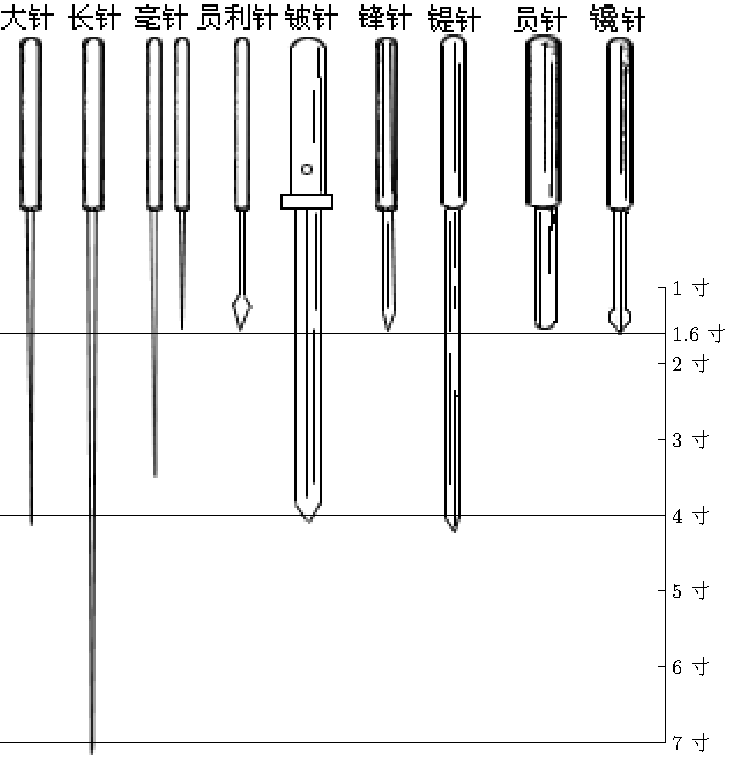
\includegraphics[width=0.50\textwidth]{九针图.pdf}\\
  \caption{九针图}\label{fig:九针图}
\end{figure}

\biaoti{【临证指要】}

\xiaobt{九针的应用}

九针,因其形状、长短等不同,在临床上的用途也各有不同。如《灵枢·官针》所说:“九针之宜,各有所为,长短大小,各有所施也。”《灵枢·刺节真邪》亦说:“刺痈者用铍针,刺大者用锋针,刺小者用圆利针,刺热者用镵针,刺寒者用毫针也。”现将《内经》所论概括如下:

(1)因病选针:病证有表里寒热虚实之异,则针有长短大小宽窄之殊。以表里深浅言,病在皮肤、分肉、脉络等表浅部位者,宜选用镵针、圆针和锋针;病在骨隙关节、脏腑等较深部位者,宜选用圆利针、长短和大针;病在皮肤、分肉,或病痹气痛不去者,因病情较轻而宜选用较小的圆针、毫针;病为大脓,或在五脏,或水肿不能过关节者,因病情较重而宜选用较大的铍针、锋针、大针。以寒热虚实言,表热轻浅,宜选用镵针、锋针;里热痈肿,宜选用锋针、铍针;正气不足者,宜选用𫔂针、圆针、毫针;邪气有余者,宜选用铍针、锋针、圆利针。

(2)因针施病:镵针:浅刺皮肤,可泻阳热邪气,主治头身之热。圆针:为按摩用针,能揩摩肌肉以泻分肉间的邪气,也可按压经络腧穴以疏通气血,还能用于放血、放水、放脓等方面。𫔂针:为按压穴位用针,能按压经脉腧穴通导气血,主治血脉病证;亦能用于探查痈脓部位深浅,开大疮口,疏通漏管的作用;因其还可扶正祛邪,故还能用于正气不足之证。锋针:能点刺放血以泻邪热,适用于血脉热瘀阻滞之顽证;还可挑破痈脓以放出脓血。铍针:为外科手术用具,可用于痈脓切排及其它手术。圆利针:用于需深刺的痈肿及暴痹。毫针:有通经络,散邪气,养正气的功用,常用于治疗寒热痛痹及邪浅在络等病证。长针:可用于治疗深部邪气及久痹。大针:主要用于利关节,泻积水。

\biaoti{【原文】}

\begin{yuanwen}
陽明多血多氣,太陽多血少氣,少陽多氣少血,太陰多血少氣,厥\sb{1}陰多血少氣,少\sb{2}陰多氣少血。故曰刺陽明出血氣,刺太陽出血惡氣,刺少陽出氣惡血,刺太陰出血惡氣,刺厥陰出血惡氣,刺少陰出氣惡血也。足陽明太陰爲表裏,少陽厥陰爲表裏,太陽少陰爲表裏,是謂足之陰陽也。手陽明太陰爲表裏,少陽心主爲表裏,太陽少陰爲表裏,是謂手之陰陽也。
\end{yuanwen}

\biaoti{【校注】}

\begin{jiaozhu}
  \item 厥:《灵枢·五音五味》作“少”,可从。
  \item 少:《灵枢·五音五味》作“厥”,可从。
\end{jiaozhu}

\biaoti{【理论阐释】}

\xiaobt{六经气血多少}

关于六经气血多少的论述,《内经》中凡三见:一见于本篇,二见于《灵枢·五音五味》,三见于《素问·血气形志篇》,但三篇所言之气血多少有异。(表\ref{tab:六经气血多少对照表})

\begin{table}[htb]%六经气血多少对照表
  \centering
  \caption{六经气血多少对照表}\label{tab:六经气血多少对照表}
  \begin{tabu}to.87\textwidth{X[-1.5c]*6{|X[c]}}
    \toprule
    \diagbox[height=2.5em]
    {篇名}{六经}& 太阳     & 少阳     & 阳明     & 少阴     & 厥阴     & 太阴     \\
    \midrule
    血气形志篇  & 多血少气 & 少血多气 & 多气多血 & 少血多气 & 多血少气 & 多气少血 \\ \hline
    五音五味    & 多血少气 & 多血少气 & 多血多气 & 多血少气 & 多气少血 & 多血少气 \\ \hline
    九针论      & 多血少气 & 少血多气 & 多血多气 & 少血多气 & 多血少气 & 多血少气 \\
    \bottomrule
  \end{tabu}
\end{table}

马莳认为,《灵枢》多误,当以《素问·血气形志篇》为正。但对六经气血多少之理,未予阐明。张志聪在注《素问·血气形志篇》中论述了此理,曰:“夫气为阳,血为阴,腑为阳,脏为阴,脏腑阴阳,雌雄相合,而气血之多少,自有常数。如太阳多血少气,则少阴少血多气;少阳少血多气,则厥阴多血少气。阳有余则阴不足,阴有余则阳不足,此天地盈虚之常数也。惟阳明则气血皆多,盖血气皆生于阳明也。”张氏之言,似亦有理,但仍有疏漏之处,即太阴气血多少尚未言及。以张氏之理推之,则太阴当为“少气少血”之经。若是,则与“脾胃者,仓廪之官,五味出焉”之旨不相符合。那么,太阴的气血究竟以多少为正?我们认为,脾胃合为“后天之本”、“气血生化之源”、太阴阳明的气血均应俱旺,才能满足机体生命活动的需要,因此,太阴之气血当为“常多血气”,或“常多血多气”。

考《太素》卷十任脉云:“太阳常多血少气,少阳常多气少血,阳明常多血少气,厥阴常多气少血,少阴常多血少气,太阴常多血少气。”杨上善注:“手足少阴、太阳多血少气,以阴多阳少也。手足厥阴、少阳多气少血,以阳多阴少也。手足太阴、阳明多血少气,以阴阳俱多谷气故也。”《太素》所载原文及杨上善之注,将太阴、阳明放在同等地位,均为“多血少气”,其立论有据,规律性强,说理充分,可以为信。

\biaoti{【临证指要】}

\xiaobt{六经气血多少理论的临床意义}

《内经》对六经气血多少的论述,反映了脏腑及其经脉的生理功能特点,对于临床具有重要指导意义。其一,指导治则治法的确立。经脉气血多少,乃脏腑精气多少的反映,因此在脏腑治疗用药时,应考虑其经脉气血多少的因素,如少气少血者,其气血易伤,治当兼顾气血之不足的生理特点。针刺方面更是如此,如太阳、厥阴为多血少气之经,针刺宜出血,忌出气;少阳、少阴为少血多气之经,针刺宜出气,忌出血;阳明、太阴为多气多血之经,针刺宜出血气。其二,指导针刺浅深及手法补泻。针刺浅深及补泻手法的运用与经脉的阴阳属性及气血多少有一定关系。根据《灵枢·经水》、《甲乙经·十二经水》等所载,其针刺浅深及留针时间,三阳经依次为少阳四分、五呼;太阳五分、七呼;阳明六分、十呼。三阴经依次为:厥阴一分、一呼或二呼;少阴二分、三呼;太阴三分、四呼。说明从总体上来看,三阳经的针刺深度和留针时间均多于三阴经。从阴、阳经分类来看,其针刺浅深和留针时间是,三阳经中,阳气多者多于阳气少者;三阴经中,阴气多者多于阴气少者。以上均可作为临床施针的参考。

\section{靈樞·血絡論}%第四節

\biaoti{【原文】}

\begin{yuanwen}
黃帝曰;願聞其奇邪而不在經者\sb{1}。岐伯曰:血絡\sb{2}是也。黃帝曰:刺血絡而仆\sb{3}者何也?血出而射\sb{4}者何也?血少黑而濁者\sb{5}何也?血出清而半爲汁\sb{6}者何也?發鍼而腫\sb{7}者何也?血出若多若少而面色蒼蒼\sb{8}者何也?發鍼而

面色不變而煩悗\sb{9}者何也?多出血而不動搖者何也?願聞其故。岐伯曰:脈氣盛而血虛者,刺之則脫氣,脫氣則仆\sb{10}。血氣俱盛而陰氣多者,其血滑,刺之則射\sb{11};陽氣畜積,久留而不瀉者,其血黑以濁,故不能射\sb{12}。新飲而液參於絡,而未合和於血也,故血出而汁別焉\sb{13};其不新飲者,身中有水,久則爲腫\sb{14}。陰氣積於陽,其氣因於絡,故刺之血未出而氣先行,故腫\sb{15}。陰陽之氣\sb{16},其新相得而未和合,因而瀉之,則陰陽俱脫,表裏相離\sb{17},故脫色而\sb{18}蒼蒼然。刺之血出多,色不變而煩悗者,刺絡而虛經,虛經之屬於陰者,陰脫故煩悗\sb{19}。陰陽相得而合爲痹者\sb{20},此爲內溢於經,外注於絡,如是者陰陽俱有餘,雖多出血而弗能虛也\sb{21}。

黃帝曰:相\sb{22}之奈何?岐伯曰:血脈者,盛堅横以赤,上下無常處\sb{23},小者如鍼,大者如筋,則而瀉之萬全也,故無失數\sb{24}矣。失數而反,各如其度\sb{25}。黃帝曰:鍼入而肉著\sb{26}者何也?岐伯曰:熱氣因於鍼則鍼熱,熱則肉著於鍼,故堅焉\sb{27}。
\end{yuanwen}

\biaoti{【校注】}

\begin{jiaozhu}
  \item 奇邪不在经者:张介宾:“奇邪,即《缪刺论》所谓奇病也。在络不在经,行无常处,故曰奇邪”。“者”后,《甲乙经》有“何也”二字,义长,可据补。
  \item 血络:即皮肤浅表视而可见之络脉。此又指皮肤浅表层有瘀血阻滞之络脉。张志聪注:“血络者,外之络脉、孙脉,见于皮肤之间,血气有所留积,则失其外内出入之机。”
  \item 刺血络而仆:刺血络出血而致昏仆倒地。
  \item 血出而射:刺血络出血,其血向外喷射。
  \item 血少黑而浊:少,《甲乙经》作“出”。可据改。血出黑而浊,即刺血络所出之血,色黑而浓稠。
  \item 血出清而半为汁:刺血络后,血出清稀,一半是澄清的汁液。
  \item 发针而肿:出针之后,局部皮肤肿胀。
  \item 面色苍苍:苍苍后,《太素》、《甲乙经》均有“然”字,可从。面色苍苍然,即面色苍白。
  \item 烦悗:悗,音义同“闷”。烦闷,即心胸烦闷。
  \item 脉气盛而血虚,刺之则脱气,脱气则仆:张志聪注:“气虽盛而血则虚者,若泻其气,则阴阳俱脱,故为仆倒。”
  \item 血气俱盛而阴气多者,其血滑,刺之则射:意为血气俱盛而阴血尤旺者,其血行滑利,刺其络则有血喷射而出。张志聪注:“俱盛者,经脉内外之血气俱盛也”。
  \item 阳气畜积,久留而不泻者,其血黑以浊,故不能射:张介宾注:“阳气久留而不泻,则阳邪日盛,阴血日枯,故血气黑以浊,所出不多,不能射也”。
  \item 新饮而液渗于络,而未合和于血也,故血出而汁别焉:意为新饮入胃,水液渗于络中而未奉心化赤为血,仍以水液(津液)状态存在,故刺络出血时,可出现既见血出又见液出的情况。张介宾注:“新饮入胃,未及变化而渗入于络,故血汁相半也。”
  \item 身中有水,久则为肿:张志聪注:“血乃水谷之津液所化,若不新饮而出而为汁者,乃身中之水也。”
  \item 阴气积于阳,其气因于络,故刺之血未出而气先行,故肿:阳,指阳分之络脉。脏腑经脉之血气汇积于皮肤肌腠之络脉,其血气随络脉而变动,针刺络脉如果气已行而血未出,瘀积于皮肤,局部肌肤就会出现肿胀。
  \item 阴阳之气:此指经脉与络脉的营卫气血。
  \item 其新相得而未和合,因而泻之,则阴阳俱脱,表里相离:张介宾注:“言血气初调,营卫甫定也。当此之时,根本未固,而妄施以泻,则阴阳表里俱致脱离,而衰危之色故见于面也”。
  \item 而:《太素》作“面”,义明,可从。
  \item 刺络而虚经,虚经之属于阴者,阴脱故烦悗:张介宾注:“取血者,刺其络也。若出血过多,必虚及于经,经之属阴者,主脏,脏虚则阴脱,故为烦悗”。
  \item 阴阳相得而合为痹:表里之邪气相合而致经络气血痹阻。
  \item 内溢于经,外注于络,如是者阴阳俱有余,虽多出血而弗能虚也:经属阴,络属阳,邪气既向内溢于经脉,又向外注于络脉,致使经络中的邪气俱盛而有余。刺其血络,虽出血量多,但所泻多为邪气,故不会招致正气受损。
  \item 相:张介宾注:“相,视也。”
  \item 血脉者,盛坚横以赤,上下无常处:瘀积的络脉,其状盛满坚硬而色红紫,或在上或在下,其位不固定。
  \item 无失数:张韦聪注:“数者,血脉出入之度数。”无失数,不要违背血脉出入之度数,亦即不要违背刺络的法度。
  \item 失数则反,各如其度:马莳注:“若失其术数,而与法相反,则凡或汁或射等证,各如其度以相应矣。”
  \item 肉著:局部肌肉紧紧裹住针身而捻转拔出困难。
  \item 热气因于针则针热,热则肉著于针,故坚焉:张介宾注:“针入而热,肉必附之,故紧涩难转而坚不可拔也。”
\end{jiaozhu}

\biaoti{【理论阐释】}

1.刺络出血法的原理及作用

络脉内连经脏,外通组织器官,是脏腑经脉气血营养脏腑组织的桥梁和枢纽。因此,络道的畅通与否是能否完成这一重要功能的先决条件。故张志聪《黄帝内经灵枢集注·血络论》说:“血络者,外之络脉、孙络,见于皮肤之间·血气有所留积,则失其外内出入之机矣。”刺络出血法的作用,概括起来主要有以下两个方面。一是刺去邪瘀,疏通络道。邪瘀阻滞络中,则络血不能正常渗灌,从而病变丛生。用刺络出血法刺出其邪瘀以达到治疗目的。二是驱除络邪,防邪传经。络与经相通,共同构成了一个封闭式循环,若有形之邪阻滞络中,则“势不能出于络外,故经盛入络,络盛返经,留连不已”(喻昌《医门法律·络脉论》)。当此之时,唯有及时运用刺络出血法祛除络中邪瘀,才能使经络正常循环。故《素问·调经论》说:“帝曰:刺留血奈何?岐伯曰:视其血络,刺出其血,无令恶血得入于经,以成其疾。”

2.刺血络的反应及其原因:本篇将刺络后的反应概括为“刺血络而仆”、“血出而射”、“血出黑而浊”、“血出清而半为汁”、“发针而肿”、“血出若多若少而面色苍苍然”、“发针而面色不变而烦悗”、“多出血而不动摇”等八种。上述八种情况,又可区分为以下两大类反应:

(1)针刺局部反应:①局部出血。血气俱盛而络中血气充足、血行流利的,可见“血出而射”;阳热蓄积,瘀积过久,可见“血出黑而浊”;刚刚饮水,水津与血尚未和合,可见“血出清而半为汁”。此外,还有血出或多或少等情况。②局部肿胀。血气积于络脉,出针时气先行,血后行而郁闭于肌腠,则可见“发针而肿”。

(2)病人神色反应:①神昏仆倒。经络中气盛血虚,刺之气随血脱,可见“刺血络而仆”。②心胸烦闷。刺络出血多,致使经虚脏衰,心神失养,可见“烦悗”。③面色苍白。阴阳未调,气血不固,妄用刺络法而使阴阳俱脱,气血耗散,可见“脱色面苍苍然”。④神色正常。邪气盛满于经络之中,正气旺盛未衰,刺之虽出血多,但属于正气驱邪外出的反应,不会伤及正气,故“多出血而不动摇”,表现为神色正常。

出现上述反应的原因,与以下四个方面的因素有关:一是病人体质的强弱。如“刺而仆”,多因体弱气血亏虚所致。临床上常见的晕针现象,亦常与此有关。“血出而射”,多因体强气血旺盛,血行流利而致。二是疾病轻重、病程长短。如“血出黑而浊”,多病程长而病情较重;“血出清而半为汁”,若非新饮,则多为“身中有水”所致。三是饮食质量及时间。如“出血清而半为汁”,多因新饮、多饮所致。四是医生技术水平和医疗态度。如“刺络而仆”,“发针而面色不变而烦悗”、“发针而肿”等反应,均与医生的技术水平和医疗态度有一定关系。

\biaoti{【临证指要】}

\xiaobt{刺络出血法的适应证及刺血度数}

《素问·血气形志篇》说:“凡治病必先去其血,乃去其所苦,伺之所欲,然后泻有余,补不足。”王冰注:“先去其血,谓见血脉盛满独异于常者乃去之,不谓常刺则先去其血也”。说明应用刺血法必须严格把握其适应证,做到有的放矢,切不可滥用。

依据《内经》所说,其刺络的适应证是血络有邪瘀阻滞,其表现是血络部可见“盛坚横以赤”、“小者如针,大者如筋”,亦即王冰所谓“血脉盛满独异于常者”。据此而刺,则攻邪而不伤正,所谓“则而泻之万全也”。因血络积聚程度的不同,刺络又有刺“结络”和刺“盛络”的区别。“结络”为瘀血留积较久较甚,刺之以去瘀血。《素问·三部九候论》说:“上实下虚,切而从之,索其结络脉,刺出其血,以见通之”。《灵枢·阴阳二十五人》亦说:“其结络者,脉结血不和,决之乃行”。“盛络”为邪气初聚,瘀血留积较轻,刺之以去邪气。《灵枢·经脉》说:“故刺诸络脉者,……甚血者,虽无结,急取之,以泻其邪而出其血。”“甚血者,虽无结”,是指络脉虽粗实胀起异于正常,但其血聚不甚明显,乃病邪初聚,血结不甚所致,急刺出血以泻其邪气。故《灵枢·根结》说:“此所谓十二经者,盛络皆为取之也”。《灵枢·脉度》亦说:“盛而血者,疾诛之。”

刺血度数,《内经》提出以“必无留血”作为标准。要做到这一点,一是“盛络皆为取之”,勿使遗漏;二是“视其血络,尽出其血”,除邪务尽。所谓“尽出其血”,《素问·刺腰痛篇》认为是“血变而止”,“见赤血而已”。可见,血色由暗转红,乃邪气已出的标志之一。以上原则,仍为今天临床所遵循。此外,还必须指出,临床上其刺血量的多少,还往往与病情轻重及所刺部位有关。故《内经》中还有“肺热病者,……刺手太阴、阳明,出血如大豆立已”,以及“顑痛,刺足阳明曲同动脉见血,立已”等记载,体现《内经》的原则性和灵活性。

\xiaojie

本章选编了《灵枢》和《素问》的四篇(段)原文,介绍了经络学说的主要内容。

十二经脉,即手足三阴三阳经,是经络的主要组成部分。其循行规律是:手三阴经,从胸走手,属脏络腑;手三阳经,从手走头,属腑络脏;足三阳经,以头走足,属腑络脏;足三阴经,从足走腹,属脏络腑。十二经首尾相贯,如环无端。十二经脉的病变包括经脉本身的病变及所联属脏腑的病变两大部分,所谓“是动病”,即经气变动而主要表现为经脉方面的病证,“所生病”,则为经气变动而主要表现为脏腑方面的病证。由于经脉内通脏腑,外连肢节,所以其病变表现的重心有经脉与脏腑的不同。

奇经八脉,包栝冲脉、任脉、督脉、带脉、阴跷、阳跷、阴维、阳维。奇经不与脏腑相通,交叉贯穿于十二经之间,具有加强经脉联系,调节各经气血阴阳的作用。其病变多表现在本经循行的部位上,如任脉为病,“男子内结七疝,女子带下瘕聚”;冲脉为病,“逆气里急”;督脉为病,“脊强反折”等。

络脉是经脉的补充,它主要分布在经脉所不到的部位,内至脏腑,外达体表,无处不到,是脏腑经络气血营养机体的桥梁与枢纽,在人体处于一个十分独特而又重要的地位。十五别络中,其十二经别络均起于四肢络穴,并联系其相表里的经脉;任脉之别散于腹;督脉之别散于头,别走足太阳经;脾之大络散布于前后胁肋。孙络的分布更为广泛,它们自大络别出后,越分越多,愈分愈细,分别弥散于经脉所属的内外区域内。

此外,本篇还讨论了六经气血多少及针刺宜忌;刺络出血法的适应证,刺血络的反应及其原因;九针的起源、命名、形状及其主治、禁忌;治疗风病、水病的俞穴;灸寒热病的取穴及方法等内容。

\zuozhe{(邱幸凡)}
\ifx \allfiles \undefined
\end{document}
\fi    % 第三章 经络
% -*- coding: utf-8 -*-
%!TEX program = xelatex
\ifx \allfiles \undefined
\documentclass[draft,12pt]{ctexbook}
%\usepackage{xeCJK}
%\usepackage[14pt]{extsizes} %支持8,9,10,11,12,14,17,20pt

%===================文档页面设置====================
%---------------------印刷版尺寸--------------------
%\usepackage[a4paper,hmargin={2.3cm,1.7cm},vmargin=2.3cm,driver=xetex]{geometry}
%--------------------电子版------------------------
\usepackage[a4paper,margin=2cm,driver=xetex]{geometry}
%\usepackage[paperwidth=9.2cm, paperheight=12.4cm, width=9cm, height=12cm,top=0.2cm,
%            bottom=0.4cm,left=0.2cm,right=0.2cm,foot=0cm, nohead,nofoot,driver=xetex]{geometry}

%===================自定义颜色=====================
\usepackage{xcolor}
  \definecolor{mybackgroundcolor}{cmyk}{0.03,0.03,0.18,0}
  \definecolor{myblue}{rgb}{0,0.2,0.6}

%====================字体设置======================
%--------------------中文字体----------------------
%-----------------------xeCJK下设置中文字体------------------------------%
\setCJKfamilyfont{song}{SimSun}                             %宋体 song
\newcommand{\song}{\CJKfamily{song}}                        % 宋体   (Windows自带simsun.ttf)
\setCJKfamilyfont{xs}{NSimSun}                              %新宋体 xs
\newcommand{\xs}{\CJKfamily{xs}}
\setCJKfamilyfont{fs}{FangSong_GB2312}                      %仿宋2312 fs
\newcommand{\fs}{\CJKfamily{fs}}                            %仿宋体 (Windows自带simfs.ttf)
\setCJKfamilyfont{kai}{KaiTi_GB2312}                        %楷体2312  kai
\newcommand{\kai}{\CJKfamily{kai}}
\setCJKfamilyfont{yh}{Microsoft YaHei}                    %微软雅黑 yh
\newcommand{\yh}{\CJKfamily{yh}}
\setCJKfamilyfont{hei}{SimHei}                                    %黑体  hei
\newcommand{\hei}{\CJKfamily{hei}}                          % 黑体   (Windows自带simhei.ttf)
\setCJKfamilyfont{msunicode}{Arial Unicode MS}            %Arial Unicode MS: msunicode
\newcommand{\msunicode}{\CJKfamily{msunicode}}
\setCJKfamilyfont{li}{LiSu}                                            %隶书  li
\newcommand{\li}{\CJKfamily{li}}
\setCJKfamilyfont{yy}{YouYuan}                             %幼圆  yy
\newcommand{\yy}{\CJKfamily{yy}}
\setCJKfamilyfont{xm}{MingLiU}                                        %细明体  xm
\newcommand{\xm}{\CJKfamily{xm}}
\setCJKfamilyfont{xxm}{PMingLiU}                             %新细明体  xxm
\newcommand{\xxm}{\CJKfamily{xxm}}

\setCJKfamilyfont{hwsong}{STSong}                            %华文宋体  hwsong
\newcommand{\hwsong}{\CJKfamily{hwsong}}
\setCJKfamilyfont{hwzs}{STZhongsong}                        %华文中宋  hwzs
\newcommand{\hwzs}{\CJKfamily{hwzs}}
\setCJKfamilyfont{hwfs}{STFangsong}                            %华文仿宋  hwfs
\newcommand{\hwfs}{\CJKfamily{hwfs}}
\setCJKfamilyfont{hwxh}{STXihei}                                %华文细黑  hwxh
\newcommand{\hwxh}{\CJKfamily{hwxh}}
\setCJKfamilyfont{hwl}{STLiti}                                        %华文隶书  hwl
\newcommand{\hwl}{\CJKfamily{hwl}}
\setCJKfamilyfont{hwxw}{STXinwei}                                %华文新魏  hwxw
\newcommand{\hwxw}{\CJKfamily{hwxw}}
\setCJKfamilyfont{hwk}{STKaiti}                                    %华文楷体  hwk
\newcommand{\hwk}{\CJKfamily{hwk}}
\setCJKfamilyfont{hwxk}{STXingkai}                            %华文行楷  hwxk
\newcommand{\hwxk}{\CJKfamily{hwxk}}
\setCJKfamilyfont{hwcy}{STCaiyun}                                 %华文彩云 hwcy
\newcommand{\hwcy}{\CJKfamily{hwcy}}
\setCJKfamilyfont{hwhp}{STHupo}                                 %华文琥珀   hwhp
\newcommand{\hwhp}{\CJKfamily{hwhp}}

\setCJKfamilyfont{fzsong}{Simsun (Founder Extended)}     %方正宋体超大字符集   fzsong
\newcommand{\fzsong}{\CJKfamily{fzsong}}
\setCJKfamilyfont{fzyao}{FZYaoTi}                                    %方正姚体  fzy
\newcommand{\fzyao}{\CJKfamily{fzyao}}
\setCJKfamilyfont{fzshu}{FZShuTi}                                    %方正舒体 fzshu
\newcommand{\fzshu}{\CJKfamily{fzshu}}

\setCJKfamilyfont{asong}{Adobe Song Std}                        %Adobe 宋体  asong
\newcommand{\asong}{\CJKfamily{asong}}
\setCJKfamilyfont{ahei}{Adobe Heiti Std}                            %Adobe 黑体  ahei
\newcommand{\ahei}{\CJKfamily{ahei}}
\setCJKfamilyfont{akai}{Adobe Kaiti Std}                            %Adobe 楷体  akai
\newcommand{\akai}{\CJKfamily{akai}}

%------------------------------设置字体大小------------------------%
\newcommand{\chuhao}{\fontsize{42pt}{\baselineskip}\selectfont}     %初号
\newcommand{\xiaochuhao}{\fontsize{36pt}{\baselineskip}\selectfont} %小初号
\newcommand{\yihao}{\fontsize{28pt}{\baselineskip}\selectfont}      %一号
\newcommand{\xiaoyihao}{\fontsize{24pt}{\baselineskip}\selectfont}
\newcommand{\erhao}{\fontsize{21pt}{\baselineskip}\selectfont}      %二号
\newcommand{\xiaoerhao}{\fontsize{18pt}{\baselineskip}\selectfont}  %小二号
\newcommand{\sanhao}{\fontsize{15.75pt}{\baselineskip}\selectfont}  %三号
\newcommand{\sihao}{\fontsize{14pt}{\baselineskip}\selectfont}%     四号
\newcommand{\xiaosihao}{\fontsize{12pt}{\baselineskip}\selectfont}  %小四号
\newcommand{\wuhao}{\fontsize{10.5pt}{\baselineskip}\selectfont}    %五号
\newcommand{\xiaowuhao}{\fontsize{9pt}{\baselineskip}\selectfont}   %小五号
\newcommand{\liuhao}{\fontsize{7.875pt}{\baselineskip}\selectfont}  %六号
\newcommand{\qihao}{\fontsize{5.25pt}{\baselineskip}\selectfont}    %七号   %中文字体及字号设置
\xeCJKDeclareSubCJKBlock{SIP}{
  "20000 -> "2A6DF,   % CJK Unified Ideographs Extension B
  "2A700 -> "2B73F,   % CJK Unified Ideographs Extension C
  "2B740 -> "2B81F    % CJK Unified Ideographs Extension D
}
%\setCJKmainfont[SIP={[AutoFakeBold=1.8,Color=red]Sun-ExtB},BoldFont=黑体]{宋体}    % 衬线字体 缺省中文字体

\setCJKmainfont{simsun.ttc}[
  Path=fonts/,
  SIP={[Path=fonts/,AutoFakeBold=1.8,Color=red]simsunb.ttf},
  BoldFont=simhei.ttf
]

%SimSun-ExtB
%Sun-ExtB
%AutoFakeBold:自动伪粗,即正文使用\bfseries时生僻字使用伪粗体;
%FakeBold:强制伪粗,即正文中生僻字均使用伪粗体
%\setCJKmainfont[BoldFont=STHeiti,ItalicFont=STKaiti]{STSong}
%\setCJKsansfont{微软雅黑}黑体
%\setCJKsansfont[BoldFont=STHeiti]{STXihei} %serif是有衬线字体sans serif 无衬线字体
%\setCJKmonofont{STFangsong}    %中文等宽字体

%--------------------英文字体----------------------
\setmainfont{simsun.ttc}[
  Path=fonts/,
  BoldFont=simhei.ttf
]
%\setmainfont[BoldFont=黑体]{宋体}  %缺省英文字体
%\setsansfont
%\setmonofont

%===================目录分栏设置====================
\usepackage[toc,lof,lot]{multitoc}    % 目录(含目录、表格目录、插图目录)分栏设置
  %\renewcommand*{\multicolumntoc}{3} % toc分栏数设置,默认为两栏(\multicolumnlof,\multicolumnlot)
  %\setlength{\columnsep}{1.5cm}      % 调整分栏间距
  \setlength{\columnseprule}{0.2pt}   % 调整分栏竖线的宽度

%==================章节格式设置====================
\setcounter{secnumdepth}{3} % 章节等编号深度 3:子子节\subsubsection
\setcounter{tocdepth}{2}    % 目录显示等度 2:子节

\xeCJKsetup{%
  CJKecglue=\hspace{0.15em},      % 调整中英(含数字)间的字间距
  %CJKmath=true,                  % 在数学环境中直接输出汉字(不需要\text{})
  AllowBreakBetweenPuncts=true,   % 允许标点中间断行,减少文字行溢出
}

\ctexset{%
  part={
    name={,篇},
    number=\SZX{part},
    format={\chuhao\bfseries\centering},
    nameformat={},titleformat={}
  },
  section={
    number={\chinese{section}},
    name={第,节}
  },
  subsection={
    number={\chinese{subsection}、},
    aftername={\hspace{-0.01em}}
  },
  subsubsection={
    number={(\chinese{subsubsection})},
    aftername={\hspace {-0.01em}},
    beforeskip={1.3ex minus .8ex},
    afterskip={1ex minus .6ex},
    indent={\parindent}
  },
  paragraph={
    beforeskip=.1\baselineskip,
    indent={\parindent}
  }
}

\newcommand*\SZX[1]{%
  \ifcase\value{#1}%
    \or 上%
    \or 中%
    \or 下%
  \fi
}

%====================页眉设置======================
\usepackage{titleps}%或者\usepackage{titlesec},titlesec包含titleps
\newpagestyle{special}[\small\sffamily]{
  %\setheadrule{.1pt}
  \headrule
  \sethead[\usepage][][\chaptertitle]
  {\chaptertitle}{}{\usepage}
}

\newpagestyle{main}[\small\sffamily]{
  \headrule
  %\sethead[\usepage][][第\thechapter 章\quad\chaptertitle]
%  {\thesection\quad\sectiontitle}{}{\usepage}}
  \sethead[\usepage][][第\chinese{chapter}章\quad\chaptertitle]
  {第\chinese{section}节\quad\sectiontitle}{}{\usepage}
}

\newpagestyle{main2}[\small\sffamily]{
  \headrule
  \sethead[\usepage][][第\chinese{chapter}章\quad\chaptertitle]
  {第\chinese{section}節\quad\sectiontitle}{}{\usepage}
}

%================ PDF 书签设置=====================
\usepackage{bookmark}[
  depth=2,        % 书签深度 2:子节
  open,           % 默认展开书签
  openlevel=2,    % 展开书签深度 2:子节
  numbered,       % 显示编号
  atend,
]
  % 相比hyperref,bookmark宏包大多数时候只需要编译一次,
  % 而且书签的颜色和字体也可以定制。
  % 比hyperref 更专业 (自动加载hyperref)

%\bookmarksetup{italic,bold,color=blue} % 书签字体斜体/粗体/颜色设置

%------------重置每篇章计数器,必须在hyperref/bookmark之后------------
\makeatletter
  \@addtoreset{chapter}{part}
\makeatother

%------------hyperref 超链接设置------------------------
\hypersetup{%
  pdfencoding=auto,   % 解决新版ctex,引起hyperref UTF-16预警
  colorlinks=true,    % 注释掉此项则交叉引用为彩色边框true/false
  pdfborder=001,      % 注释掉此项则交叉引用为彩色边框
  citecolor=teal,
  linkcolor=myblue,
  urlcolor=black,
  %psdextra,          % 配合使用bookmark宏包,可以直接在pdf 书签中显示数学公式
}

%------------PDF 属性设置------------------------------
\hypersetup{%
  pdfkeywords={黄帝内经,内经,内经讲义,21世纪课程教材},    % 关键词
  %pdfsubject={latex},        % 主题
  pdfauthor={主编:王洪图},   % 作者
  pdftitle={内经讲义},        % 标题
  %pdfcreator={texlive2011}   % pdf创建器
}

%------------PDF 加密----------------------------------
%仅适用于xelatex引擎 基于xdvipdfmx
%\special{pdf:encrypt ownerpw (abc) userpw (xyz) length 128 perm 2052}

%仅适用于pdflatex引擎
%\usepackage[owner=Donald,user=Knuth,print=false]{pdfcrypt}

%其他可使用第三方工具 如:pdftk
%pdftk inputfile.pdf output outputfile.pdf encrypt_128bit owner_pw yourownerpw user_pw youruserpw

%=============自定义环境、列表及列表设置================
% 标题
\def\biaoti#1{\vspace{1.7ex plus 3ex minus .2ex}{\bfseries #1}}%\noindent\hei
% 小标题
\def\xiaobt#1{{\bfseries #1}}
% 小结
\def\xiaojie {\vspace{1.8ex plus .3ex minus .3ex}\centerline{\large\bfseries 小\ \ 结}\vspace{.1\baselineskip}}
% 作者
\def\zuozhe#1{\rightline{\bfseries #1}}

\newcounter{yuanwen}    % 新计数器 yuanwen
\newcounter{jiaozhu}    % 新计数器 jiaozhu

\newenvironment{yuanwen}[2][【原文】]{%
  %\biaoti{#1}\par
  \stepcounter{yuanwen}   % 计数器 yuanwen+1
  \bfseries #2}
  {}

\usepackage{enumitem}
\newenvironment{jiaozhu}[1][【校注】]{%
  %\biaoti{#1}\par
  \stepcounter{jiaozhu}   % 计数器 jiaozhu+1
  \begin{enumerate}[%
    label=\mylabel{\arabic*}{\circledctr*},before=\small,fullwidth,%
    itemindent=\parindent,listparindent=\parindent,%labelsep=-1pt,%labelwidth=0em,
    itemsep=0pt,topsep=0pt,partopsep=0pt,parsep=0pt
  ]}
  {\end{enumerate}}

%===================注解与原文相互跳转====================
%----------------第1部分 设置相互跳转锚点-----------------
\makeatletter
  \protected\def\mylabel#1#2{% 注解-->原文
    \hyperlink{back:\theyuanwen:#1}{\Hy@raisedlink{\hypertarget{\thejiaozhu:#1}{}}#2}}

  \protected\def\myref#1#2{% 原文-->注解
    \hyperlink{\theyuanwen:#1}{\Hy@raisedlink{\hypertarget{back:\theyuanwen:#1}{}}#2}}
  %此处\theyuanwen:#1实际指thejiaozhu:#1,只是\thejiaozhu计数器还没更新,故使用\theyuanwen计数器代替
\makeatother

\protected\def\myjzref#1{% 脚注中的引用(引用到原文)
  \hyperlink{\theyuanwen:#1}{\circlednum{#1}}}

\def\sb#1{\myref{#1}{\textsuperscript{\circlednum{#1}}}}    % 带圈数字上标

%----------------第2部分 调整锚点垂直距离-----------------
\def\HyperRaiseLinkDefault{.8\baselineskip} %调整锚点垂直距离
%\let\oldhypertarget\hypertarget
%\makeatletter
%  \def\hypertarget#1#2{\Hy@raisedlink{\oldhypertarget{#1}{#2}}}
%\makeatother

%====================带圈数字列表标头====================
\newfontfamily\circledfont[Path = fonts/]{meiryo.ttc}  % 日文字体,明瞭体
%\newfontfamily\circledfont{Meiryo}  % 日文字体,明瞭体

\protected\def\circlednum#1{{\makexeCJKinactive\circledfont\textcircled{#1}}}

\newcommand*\circledctr[1]{%
  \expandafter\circlednum\expandafter{\number\value{#1}}}
\AddEnumerateCounter*\circledctr\circlednum{1}

% 参考自:http://bbs.ctex.org/forum.php?mod=redirect&goto=findpost&ptid=78709&pid=460496&fromuid=40353

%======================插图/tikz图========================
\usepackage{graphicx,subcaption,wrapfig}    % 图,subcaption含子图功能代替subfig,图文混排
  \graphicspath{{img/}}                     % 设置图片文件路径

\def\pgfsysdriver{pgfsys-xetex.def}         % 设置tikz的驱动引擎
\usepackage{tikz}
  \usetikzlibrary{calc,decorations.text,arrows,positioning}

%---------设置tikz图片默认格式(字号、行间距、单元格高度)-------
\let\oldtikzpicture\tikzpicture
\renewcommand{\tikzpicture}{%
  \small
  \renewcommand{\baselinestretch}{0.2}
  \linespread{0.2}
  \oldtikzpicture
}

%=========================表格相关===============================
\usepackage{%
  multirow,                   % 单元格纵向合并
  array,makecell,longtable,   % 表格功能加强,tabu的依赖
  tabu-last-fix,              % "强大的表格工具" 本地修复版
  diagbox,                    % 表头斜线
  threeparttable,             % 表格内脚注(需打补丁支持tabu,longtabu)
}

%----------给threeparttable打补丁用于tabu,longtabu--------------
%解决方案来自:http://bbs.ctex.org/forum.php?mod=redirect&goto=findpost&ptid=80318&pid=467217&fromuid=40353
\usepackage{xpatch}

\makeatletter
  \chardef\TPT@@@asteriskcatcode=\catcode`*
  \catcode`*=11
  \xpatchcmd{\threeparttable}
    {\TPT@hookin{tabular}}
    {\TPT@hookin{tabular}\TPT@hookin{tabu}}
    {}{}
  \catcode`*=\TPT@@@asteriskcatcode
\makeatother

%------------设置表格默认格式(字号、行间距、单元格高度)------------
\let\oldtabular\tabular
\renewcommand{\tabular}{%
  \renewcommand\baselinestretch{0.9}\small    % 设置行间距和字号
  \renewcommand\arraystretch{1.5}             % 调整单元格高度
  %\renewcommand\multirowsetup{\centering}
  \oldtabular
}
%设置行间距,且必须放在字号设置前 否则无效
%或者使用\fontsize{<size>}{<baseline>}\selectfont 同时设置字号和行间距

\let\oldtabu\tabu
\renewcommand{\tabu}{%
  \renewcommand\baselinestretch{0.9}\small    % 设置行间距和字号
  \renewcommand\arraystretch{1.8}             % 调整单元格高度
  %\renewcommand\multirowsetup{\centering}
  \oldtabu
}

%------------模仿booktabs宏包的三线宽度设置---------------
\def\toprule   {\Xhline{.08em}}
\def\midrule   {\Xhline{.05em}}
\def\bottomrule{\Xhline{.08em}}
%-------------------------------------
%\setlength{\arrayrulewidth}{2pt} 设定表格中所有边框的线宽为同样的值
%\Xhline{} \Xcline{}分别设定表格中水平线的宽度 makecell包提供

%表格中垂直线的宽度可以通过在表格导言区(preamble),利用命令 !{\vrule width1.2pt} 替换 | 即可

%=================图表设置===============================
%---------------图表标号设置-----------------------------
\renewcommand\thefigure{\arabic{section}-\arabic{figure}}
\renewcommand\thetable {\arabic{section}-\arabic{table}}

\usepackage{caption}
  \captionsetup{font=small,}
  \captionsetup[table] {labelfont=bf,textfont=bf,belowskip=3pt,aboveskip=0pt} %仅表格 top
  \captionsetup[figure]{belowskip=0pt,aboveskip=3pt}  %仅图片 below

%\setlength{\abovecaptionskip}{3pt}
%\setlength{\belowcaptionskip}{3pt} %图、表题目上下的间距
\setlength{\intextsep}   {5pt}  %浮动体和正文间的距离
\setlength{\textfloatsep}{5pt}

%====================全文水印==========================
%解决方案来自:
%http://bbs.ctex.org/forum.php?mod=redirect&goto=findpost&ptid=79190&pid=462496&fromuid=40353
%https://zhuanlan.zhihu.com/p/19734756?columnSlug=LaTeX
\usepackage{eso-pic}

%eso-pic中\AtPageCenter有点水平偏右
\renewcommand\AtPageCenter[1]{\parbox[b][\paperheight]{\paperwidth}{\vfill\centering#1\vfill}}

\newcommand{\watermark}[3]{%
  \AddToShipoutPictureBG{%
    \AtPageCenter{%
      \tikz\node[%
        overlay,
        text=red!50,
        %font=\sffamily\bfseries,
        rotate=#1,
        scale=#2
      ]{#3};
    }
  }
}

\newcommand{\watermarkoff}{\ClearShipoutPictureBG}

\watermark{45}{15}{草\ 稿}    %启用全文水印

%=============花括号分支结构图=========================
\usepackage{schemata}

\xpatchcmd{\schema}
  {1.44265ex}{-1ex}
  {}{}

\newcommand\SC[2] {\schema{\schemabox{#1}}{\schemabox{#2}}}
\newcommand\SCh[4]{\Schema{#1}{#2}{\schemabox{#3}}{\schemabox{#4}}}

%=======================================================

\begin{document}
\pagestyle{main2}
\fi
\chapter{病因病机}%第四章

病因,即生病的原因,也就是破坏人体相对动态平衡而导致发生疾病的原因。《内经》所论述的病因有外感时邪、情志过激、饮食失调、劳逸失度、起居无节、跌仆损伤以及病气遗传等方面。病机,就是疾病发生发展变化的规律。包括阴阳盛衰、正邪虚实、升降出入失调等。有关病因、病机的记载,主要见于《素问·生气通天论》、《素问·玉机真脏论》、《素问·至真要大论》、《素问·举痛论》以及《灵枢·百病始生》等篇。

\section{素問·生氣通天論}%第一节

\biaoti{【原文】}

\begin{yuanwen}
黃帝曰:夫自古通天者,生之本,本於陰陽\sb{1}。天地之間,六合\sb{2}之内,其氣九州\sb{3}、九竅、五藏、十二節\sb{4},皆通乎天氣,其生五,其氣三\sb{5},数犯此者,則邪氣傷人,此壽命之本也。

蒼天之氣,清淨則志意治\sb{6},順之則陽氣固,雖有賊邪\sb{7},弗能害也。此因時之序\sb{8}。故聖人傳精神\sb{9},服天氣\sb{10},而通神明\sb{11}。失之,則內閉九竅,外壅肌肉,衛氣散解\sb{12},此谓自傷,氣之削\sb{13}也。
\end{yuanwen}

\biaoti{【校注】}

\begin{jiaozhu}
  \item 生之本,本于阴阳:生命的根本在于枬阳双方的协调统一。
  \item 六合:指东、南、西、北、上、下六方,即整个宇宙。
  \item 九州:王冰注:“九州,谓冀、兖、青、徐、扬、荆、豫、梁、雍也。”地有九州,人有九窍。然俞樾《内经辩言》注:“九州即九窍,……古谓窍为州。”如此,“九州”与下文“九窍”义重,疑衍。
  \item 十二节:即双侧腕、肘、肩、踝、膝、髋等十二个大关节。
  \item 其生五,其气三:其,指自然界的阴阳。五,即木火土金水五行。三,即三阴三阳。全句意为自然界的阴阳化生木火土金水五行,分为三阴三阳。
  \item 清净则志意治:净,通静。志意,指人的精神活动。治,正常。即自然界阴阳之气清静而无异常变化,则有利于人的精神保持正常。
  \item 贼邪:贼,伤害也。贼邪,即伤害人的邪气。
  \item 此因时之序:因,顺也。意即顺应四时气候变化的规律而养生。
  \item 传精神:俞樾《内经辩言》注:“传,读为抟,聚也。”传精神,即聚精神,全神贯注之义。
  \item 服天气:服,顺也。意即顺应自然界阴阳之气的变化。
  \item 通神明:通,此处作统一解。神明,即阴阳变化。通神明,言人体阴阳之气与自然界阴阳之气变化统一起来。
  \item 卫气散解:指卫气离散耗解而不固。
  \item 气之削:即阳气被削弱。
\end{jiaozhu}

\biaoti{【理论阐释】}

\xiaobt{关于“生气通天”}

本节重点阐述人体生命的根本在于阴阳二气的协调,而且人体阴阳之气与自然界阴阳是相互通应的,亦要达到协调统一。所以养生应顺应天地阴阳的变化,如《素问·四气调神大论》中“春夏养阳,秋冬养阴”之法。传精神,服天气,而通神明”,乃本篇眼目,昭示养生要旨,内则精神专一,外则顺应自然,保持人与自然的和谐,如此“则阳气固,虽有贼邪弗能害也。”若违背了这一规律,内有脏腑阴阳气血失调,九窍功能障碍;外有肌肉壅阻而不滑利,卫气不固而腠理疏松,则邪气为害,正气削弱,疾病丛生而短折寿命。

“天人相应”为《内经》基本学术思想之一,而“生气通天”是《内经》中“天人相应”观的组成部分。说明人体内的各种生理机能无不与自然界息息相通。如《灵枢·岁露论》曰:“人与天地相参也,与日月相应也;”《素问·金匮真言论》指出:“五脏应四时,各有收受。”《灵枢·五癃津液别》论津液气化受四时影响,“天暑衣厚则腠理开,故汗出”;“天寒则腠理闭,气湿不行,水下留于膀胱,则为溺与气。”《素问·八正神明论》认为血气的运行、盛衰变化与月亮盈亏关系甚密,谓“月始生,则血气始精,卫气始行;月郭满,则血气实,肌肉坚;月郭空,则肌肉减,经络虚,卫气去。”人生存于自然之中,与自然环境有如此息息相关之联系,故在此特别强调了养生必须以“生气通天”为要领。

\biaoti{【原文】}

\begin{yuanwen}
陽氣者,若天與日,失其所\sb{1}則折壽而不彰\sb{2}。故天運\sb{3}當以日光明。是故陽因而上\sb{4},衛外者也。
\end{yuanwen}

\biaoti{【校注】}

\begin{jiaozhu}
  \item 失其所:所,场所。谓阳气运行、作用失常,失去其应居之所。
  \item 折寿而不彰:折寿,即短寿;不彰,不显著。指人身若阳气功能失常,可导致短折寿命的结果。高世栻注:“通体之气,经脉之气,各有其所。若失其所,则运行者不周于通体,旋转者不循行于经脉,故短折其寿,而不彰著于人世矣。”
  \item 天运:即天体的运行。
  \item 阳因而上:因,顺应,依顺。言阳气顺应其上升外越之性,而具有卫外的作用。
\end{jiaozhu}

\biaoti{【理论阐释】}

\xiaobt{阳气的重要作用}

本节把人之阳气比做天体中的太阳,据此可见,人之阳气具有天之阳气诸多特点和功用。天之阳气能给自然界带来光明、温暖。主司天体的运行,可蒸腾气化水液,使万物生长化收藏;没有太阳,也就没有自然万物蓬勃之象。比类于人体,则人之阳气具有护卫生命,促进机体生命活动运转不息的作用,若阳气“失其所”,则人之寿命不保而早夭。人体之温暖,五脏功能之运转,津液之气化,对外界虚邪贼风之抵御,均赖阳气的温煦和推动。可见,在人体的阴阳平衡中,阳气起着主导的作用。这种重视阳气的观点启发后世医家,并成为温补学派的重要理论依据。明代医家张介宾在《类经附翼·求正录》中说:“阳化气,阴成形。形本属阴,而凡通体之温者,阳气也;一生之活者,阳气也;五官五脏之神明不测者,阳气也。及其既死,则身冷如冰,灵觉尽灭,形固存而气则去,此以阳脱在前,而阴留在后。”强调“天之运,人之命,天之根本,总在太阳无两也。”并进而提出了“天之大宝,只此一丸红日;人之大宝,只此一息真阳”(《类经附翼·大宝论》)的著名论点。

\biaoti{【原文】}

\begin{yuanwen}
因於寒,欲如運樞\sb{1},起居如驚,神氣乃浮\sb{2};因於暑,汗,煩則喘喝,靜則多言\sb{3},體若燔炭,汗出而散;因於濕,首如裹,濕熱不攘\sb{4},大筋緛短,小筋㢮長\sb{5},緛短爲拘,㢮長爲痿;因於氣\sb{6},爲腫。四維相代\sb{7},陽氣乃竭。

陽氣者,煩勞則張\sb{8},精絕,辟積\sb{9}於夏,使人煎厥\sb{10}。目盲不可以視,耳閉不可以聽,潰潰乎若壞都,汩汩乎不可止\sb{11}。陽氣者,大怒則形氣絕\sb{12},而血菀\sb{13}上,使人薄厥\sb{14}。有傷於筋,縱,其若不容\sb{15}。汗出偏沮\sb{16},使人偏枯。汗出見濕,乃生痤疿\sb{17}。高梁之變,足生大丁\sb{18},受如持虚\sb{19}。勞汗當風,寒薄爲皶\sb{20},鬱乃痤。

陽氣者,精則養神,柔則養筋\sb{21}。開合不得,寒氣從之,乃生大僂\sb{22};陷脈爲瘻\sb{23},留連肉腠,俞氣化薄\sb{24},傳爲善畏,及爲驚駭\sb{25};營氣不從,逆於肉理,乃生癰腫;魄汗\sb{26}未盡,形弱而氣爍\sb{27},穴俞以閉,發爲風瘧\sb{28}。

故風者,百病之始也,清靜則肉腠閉拒,雖有大風苛毒\sb{29},弗之能害\sb{30}。此因時之序也。故病久則傳化,上下不並\sb{31},良醫弗爲。故陽畜稹病死,而陽氣當隔,隔者當寫\sb{32}。不亟正治,粗乃敗之\sb{33}。

故陽氣者,一日而主外,平旦人氣生,日中而陽氣隆,日西而陽氣已虛,氣門\sb{34}乃閉。是故暮而收拒,無擾筋骨,無見霧露,反此三時\sb{35},形乃困薄\sb{36}。
\end{yuanwen}

\biaoti{【校注】}

\begin{jiaozhu}
  \item 欲如运枢:运,运转。枢,户枢,即门轴。欲如运枢,是指卫阳之气如户枢般开合运转自如。
  \item 起居如惊,神气乃浮:惊,卒暴之意。神气,即指阳气。浮,浮越于表。意为生活起居正常规律被扰,邪气侵犯,卫阳之气则上浮与邪气抗争。
  \item 烦则喘喝,静则多言:烦,烦躁不安。喘喝,气喘息急,喝喝有声。烦则喘喝,为阳热内盛所致;静,相对烦而言,指神昏嗜卧。多言,如神昏谵语、郑声之类。静则多言,为暑邪伤神所致。
  \item 攘:除也。
  \item 大筋緛短,小筋拖长:緛,收缩。㢮,同弛,松弛。本句作互文解,即太筋、小筋或为收缩变短,或为弛缓变长。
  \item 气:即风。高世栻注:“气,犹风也,《阴阳应象大论》云:‘阳之气,以天地之疾风名之。’故不言风而言气。”
  \item 四维相代:四维,四方四时,此处指上文所言的风寒暑湿等四时邪气。代,更代。意为寒、暑、湿、风(气)四种邪气更替伤人。
  \item 张:鸱张亢盛。
  \item 辟积:辟,通襞,即衣裙褶。辟积,重复之义。
  \item 煎厥;病名。指过度烦劳,阳气鸱张亢盛,火炎则水干,阴精虚衰,又逢盛夏阳热之气,则两热相合,如煎如熬,以致阴气竭绝而昏厥的病证。
  \item 溃溃乎若坏都,汩汩乎不可止:溃溃,是形容洪水泛滥的样子。都,防水之堤。汩汩,水急流的声音。本句以洪水决堤来形容煎厥发病来势凶猛发展迅速的病证特点。
  \item 形气绝:形,即形体,此处主要指脏腑经络。绝,阻滞隔绝。马莳注谓:此“绝”是“阻绝之义,非断绝之谓。”形气绝,即脏腑经络之气阻绝不通。
  \item 菀:同郁。
  \item 薄厥:病名。指大怒而气血上逆所致的昏厥病证。张介宾注:“相迫曰薄,气逆曰厥,气血俱乱,故为薄厥。”
  \item 不容:容,通“用”。不容,即不用,指肢体不能随意运动。
  \item 汗出偏沮:沮,阻也,阻止。汗出偏沮,指汗出受阻而半侧身体无汗的症状。
  \item 痤疿:痤,即小疖。疿,即汗疹,痱子。
  \item 高梁之变,足生大丁:高,通膏,即脂膏类食物。梁,通粱,即精细的食物。膏粱,在此指肥甘厚味。足,俞樾《内经辨言》云:疑‘是’字之误。上云乃生痤疿,此云是生大丁,语意一律,‘是’误为足”。胡澍《素问校义》亦云:“足,当作是字之误也。是,犹则也。”丁,通疔,此泛指疮疡。吴昆注:“膏粱之人,内多滞热,故其病变,能生大疔。”
  \item 受如持虚:形容得病容易,犹如持空虚之器受物一样。
  \item 皶:即生长于面部的粉刺;若生于鼻部则为酒齄鼻。
  \item 精则养神,柔则养筋:当作“养神则精,养筋则柔”解。精,指精神爽慧。柔,即筋脉柔和,活动自如。此句提示阳气具有温养精神、筋脉作用。
  \item 大偻:偻,曲背之义。大偻,指阳气不能温养筋脉导致形态伛偻,不能直立的病证。
  \item 陷脉为瘘:陷脉,指邪气内陷经脉。瘘,瘘管,即病理性管道。
  \item 俞气化薄:俞,同腧,即腧穴,为经脉气血输注之处。化,传化、传入的意思。薄,迫也。俞气化薄,指邪气从腧穴传入而内迫五脏。
  \item 传为善畏,及为惊骇:五脏主藏神,脏气被邪所迫,阳气不能养神,故见心神不安之善畏、惊骇。
  \item 魄汗:魄,通白,魄汗即白汗。白汗,指汗出不因暑热所致,即自汗也。
  \item 形弱而气烁:形弱,在此指腠理不固,自汗出而易感受外邪,形体虚弱。烁,消烁。气烁,此指阳气被邪热所消耗。
  \item 风疟:疟疾之一,因感受风邪,寒热往来,恶风汗出而名之。
  \item 大风苛毒:苛,暴也。大风苛毒,指致病性强的病邪。
  \item 弗之能害:即“弗能害之”,弗,通勿。
  \item 上下不并:并,交并,交通之意。上下不并,指人体阳气上部与下部不相交通,相互阻隔的病理变化。
  \item 阳气当隔,隔者当写:前一“当”字,通挡。阳气挡隔,对此应当采用泻法,祛火以使蓄积的阳气得以畅通。
  \item 不亟正治,粗乃败之:亟,急也。粗,粗工,即医疗水平低劣的医生。全句意为不能迅速给予正确治疗,这样水平低劣的医生只能使病情败坏、恶化。
  \item 气门:此处指汗孔。王冰注:“所以发泄经脉营卫之气,故谓之气门也。”
  \item 三时:即上文的平旦、日中、日西。
  \item 形乃困薄,指形体困顿而衰薄。马莳注:“未免困窘而衰薄矣。”
\end{jiaozhu}

\biaoti{【理论阐释】}

1.阳气的生理功能

(1)“阳气者,精则养神,柔则养筋”

提示阳气的温养作用,阳气旺盛可使人精神聪慧、饱满,筋脉柔软屈伸自如。若阳气发生病变,则温养作用下降,精神、筋脉失养出现病变。如煎厥之病,因烦劳阳气亢盛精绝而至精神昏聩,再如薄厥,因大怒阳气上逆迫血上行,至血菀伤神伤筋,神伤则厥,筋伤则纵而不用;大偻之病,乃阳气不得养筋所致;魄汗则为阳气不能温固肌表所起。

(2)阳气随昼夜阴阳消长而变化

阳气在一昼夜中有生发,隆盛、虚衰的变化规律,人身阳气与自然界阴阳变化息息相关。提示人要随自然界的阴阳变化来调节生活起居,以保持阳气的充沛,防止疾病的发生。病理上,《灵枢·顺气一日分为四时》有“旦慧、昼安、夕加、夜甚”的疾病变化规律,其内在机制也是阳气昼夜消长的节律性变化。这种认识与现代人体生物钟理论相似,值得进一步探讨和研究。

2.阳气的病理

(1)阳气卫外失常,外邪侵袭

寒邪易伤阳气,故首论“因于寒”;暑为阳邪,两伤气津,实证是邪热内盛而多汗烦喘,虚证则神失所养而神昏谵语;湿邪重浊,困遏阳气,清阳不升,故头重,湿邪郁而化热,流连筋脉,致阳气不能温养,故或为挛急,或为筋痿;风性轻扬,易致头面浮肿。如风寒暑湿,交替为病,阳气反复受损,可使阳气衰竭。

(2)阳亢精绝

平素烦劳过度,阳气过亢,虚火上炎,阴精亏损,复加暑热煎灼,致阴精衰惫,发生突然昏厥,古人名为“煎厥”。其临床表现除昏厥外,还有耳闭、目盲。此病虽来势骤急,但以阴精亏损为本,故为至虚危候。

(3)阳气厥逆

由大怒而致气上逆,血随气升,气血逆乱,出现突然昏厥,古人名为“薄厥”。其临床表现除昏厥外,可见筋脉弛纵不收,类似于现代脑中风。其发病暴卒,故其初病为气血壅阻之实证。

(4)阳气偏阻

阳气不足,不能温运全身,偏阻一侧,表现为半侧身体汗出,半侧无汗,有可能出现局部肢体枯萎不用的病证。

(5)阳气郁遇

汗出而阳气宣泄之时,猝被湿邪所郁遏,宣泄不畅,易生疖子、痱子。或形劳汗出,坐卧当风,风寒迫聚于皮腠,形成粉刺,郁而化热而成疮疖。

(6)阳热内盛

嗜食膏粱厚味,阳热蓄积,热毒逆于肉里,易生疔疮,而腐肉酿脓。

(7)阳气开合不得

阳气不足,邪气入里留恋不去,会导致各种病证。如邪入筋,阳虚寒邪痹阻于背,筋失温养,不能运动自如,出现背曲不能直立之症。邪入脉中,阳虚邪陷经脉,经脉败漏,日久成痿管,久不收口。邪入脏腑,阳虚邪气留恋肉腠,由俞穴侵入,内传迫及五脏,影响其藏神功能,而出现善畏、惊骇等症。邪入肉里,营卫失调,营气不从,阻逆于肌肉之间,发生痈肿。邪入俞穴,阳气被热邪所耗伤,汗出不止,风邪入侵,俞穴闭阻,发生风疟。

(8)阳气阻隔,上下不相交通

阳气蓄积于一处则病情危重,当急用泻法以祛除实火,疏通阳气,当能挽救。

3.对“因于寒,欲如运枢”的理解

“因于寒,欲如运枢”历代有不同见解。王冰注云:“言因天之寒,当深居周密,如枢纽之内动;不当烦扰筋骨,使阳气发泄于皮肤,而伤于寒毒也。”认为是指冬季不宜剧烈运动,只能像转动门轴那样活动一下关节即可。此为一。《新校正》云:“按全元起本作‘连枢’。元起云:阳气定如连枢者,动系也。”据此,“欲如运枢”当作“定如连枢”,意谓阳气被寒邪束缚,不得畅运,犹如门枢被固定,开合不得。此为二;明·吴昆则将“欲如运枢,起居如惊,神气乃浮”三句移至上文“阳因而上,卫外者也”之后,而把“体若燔炭,汗出而散”移至“因于寒”下,此为三。第三种解释即补充说明了阳气的卫外作用,又将受于寒邪后机体的抵抗能力和症状表现凸现出来,比较符合临床实际。

\biaoti{【临证指要】}

1.薄厥和煎厥

薄厥来势凶猛,可见突然昏愦,目闭耳聋,筋脉弛纵,半身不遂,口舌歪斜,二便失禁。类似于临床中风病,这是中医对脑中风证的最早记载。张介宾曰:“厥逆之证,危证也。盖厥者,尽也;逆者,乱也。即气血败乱之谓也。故《内经》特重而详言之”(《景岳全书·杂证谟》)。当此之时,可用镇肝熄风汤合安宫牛黄丸治之,待病情控制后再以补阳还五汤治其“有伤于筋,纵,其若不容”的瘫痪症状。张介宾又认为薄厥亦有轻证,如“气实而厥者,其形气愤然勃然,脉沉弦而滑,胸膈喘满,此气逆证也。经曰:大怒则形气绝,而血苑于上,即此类也。治宜以排气饮或四磨饮,或八味顺气丸,苏合香丸之类,先顺其气,然后随其虚实而调理之”(《景岳全书·杂证谟》)。这类患者未必有筋脉弛纵证候。其证类似于今之癔病。

煎厥一证强调了阴虚阳亢的内在因素,又突出了暑热相合的外因,这很符合临床暑厥的病证。暑厥的患者多为体质虚弱,能冬不能夏的老人、幼儿、久病或产后妇女,临床常见暑厥病势凶猛,而无手足弛缓的瘫痪症状,但亦有老年患者,病情复杂,暑厥时又并发脑血管意外,则可有手足瘫痪的表现,临床须仔细观察,及时抢救。

2.“因于湿,首如裹,湿热不攘,大筋緛短,小筋弛长”

临床一般遇筋脉病变常以肝风内动、热极生风或外感风邪猝伤筋脉辨证,而本句原文则提示湿邪亦可致筋脉病变,由于湿为阴邪,若留连日久,阳气被阻或损伤,则筋脉失养,而有拘挛弛缓之症。此种观点在《内经》中还见于《至真要大论》“诸痉项强,皆属于湿。”故治疗此类筋脉病变可用祛湿之法,如《丹溪心法》中加味二妙散治疗筋脉弛缓;王海藏用神术汤加羌活、独活、麻黄治筋脉拘挛而发热无汗反恶寒的刚痉;用白术汤加桂心、黄芪治疗筋脉拘急而发热汗出不恶寒的柔痉。

3.“因于暑,汗,烦则喘喝;静则多言”

感受署邪之后,汗出是其主症之一。“烦则喘喝;静则多言”,张介宾分析:“暑有阴阳之证,阳证因于中热,阴证因于中寒……此节所言,言暑之阳者也。故为汗出烦躁,为喘,为大声呼喝。若其静者,亦不免于多言。盖邪热伤阴,精神内乱,故言无伦次也。”暑热熏蒸,汗出烦躁喘喝,此为实证;若暑热过伤心神,神伤嗜卧,表情淡漠,郑声多言,多为气阴两虚之证。实证宜祛暑清热;虚证应清暑益气。

\biaoti{【原文】}

\begin{yuanwen}
岐伯曰:陰者藏精而起亟\sb{1}也;陽者衛外而爲固也。陰不勝其陽,則脈流薄疾\sb{2},並乃狂\sb{3};陽不勝其陰,則五藏氣爭\sb{4},九竅不通。是以聖人陳陰陽,筋脈和同\sb{5},骨髓堅固,氣血皆從。如是則內外調和,邪不能害,耳目聰明,氣立如故\sb{6}。

風客淫氣,精乃亡\sb{7},邪傷肝也。因而飽食,筋脈横解\sb{8},腸澼爲痔\sb{9};因而大飲,則氣逆;因而強力\sb{10},腎氣乃傷,高骨\sb{11}乃壞。

凡陰陽之要,陽密乃固\sb{12}。兩者不和,若春無秋,若冬無夏,因而和之,是謂聖度。故陽強不能密,陰氣乃絕\sb{13};陰平陽秘,精神乃治\sb{14};陰陽離決,精氣乃絕\sb{15}。

因於露風\sb{16},乃生寒熱。是以春傷於風,邪氣留連,乃爲洞泄\sb{17};夏傷於暑,秋爲痎瘧、秋傷於濕,上逆而咳\sb{19},發爲痿厥\sb{20};冬傷於寒,春必溫病\sb{21}。四時之氣,更傷五藏\sb{22}。
\end{yuanwen}

\biaoti{【校注】}

\begin{jiaozhu}
  \item 起亟:亟,频数.起亟,指阴精不断地起而与阳气相应,说明阴为阳之基。
  \item 脉流薄疾:薄,迫也。脉流薄疾,指阳气亢盛,使脉中气血流动急迫而快疾。
  \item 并乃狂:并,交并,引申为重复、加甚之意。并乃狂,指阳气亢盛而致神志狂乱。
  \item 五脏气争:争,不和之意。五脏气争,指五脏功能失调,气机失和。
  \item 筋脉和同:和同,即和谐,协调。筋脉和同,指筋脉功能协调。
  \item 气立如故:立,反训为行。气立如故,指脏腑经络之气运行正常。一说气立,谓人需依赖自然四时之气才能有此生命。吴昆云:“气立者,人受天地之气以立命,故有生谓之气立。”
  \item 风客淫气,精乃亡:凤邪侵袭人体,而为淫乱之气。风为阳邪,易使阴精耗散。高世栻注:“风为阳邪,风客淫气,则阴精消烁,故精乃亡。”
  \item 筋脉横解:横,放纵的意思。解,通懈,即松弛。筋脉横解,即筋脉弛纵不收。
  \item 肠澼为痔:肠澼,即下利脓血的痢疾等病。为,与也。痔,痔疮。饮食过饱,肠胃乃伤,湿热下注则为痢疾;迫于魄门,日久成痔。
  \item 强力:勉强用力,劳力过度,又指房室太过,王冰注:“强力,谓强力入房也。”
  \item 高骨:即腰间脊骨。
  \item 阴阳之要,阳密乃固:要,关键,要领。阴精与阳气关系的关键,在于阳气致密于外,阴气才能固守于内。
  \item 阳强不能密,阴气乃绝;阳强,阳气亢盛。阳气若致密于外,则阴气能固守于内。今阳气亢盛,不能为阴气致密于外,则阴气亦不能内守而外泄,以至衰竭亡绝。张介宾注:“强,亢也。孤阳独月,不能固密,则阳气耗而竭绝矣。《痹论》曰:阴气者,静则神藏,躁则消亡。躁即阳强不密之谓。”
  \item 阴平阳秘,精神乃治:阴平阳秘为互文,即阴阳平秘。平秘,平和协调之意。治,正常。
  \item 阴阳离决,精气乃绝:离,分离。决,决裂。阴阳分离决裂,则孤阳不生独阴不长,精气无以滋生而竭绝。
  \item 露风:泛指一般外感病的致病因素,如下文所言风、暑、湿、寒诸邪。又,露,触冒。露风,即触冒风邪之意。
  \item 洞泄:指水谷不化,下利无度的重度泄泻。
  \item 痎疟:疟疾的总称。
  \item 秋伤于湿,上逆而咳:张介宾注:“湿土用事于长夏之末,故秋伤于湿也。秋气通于肺,湿郁成热,则上乘肺金,故气逆而为咳嗽。”
  \item 痿厥:偏义复词,偏在“痿”,即肢体枯萎不用的病证。
  \item 冬伤于寒,春必温病:因冬季养生不当,感受寒邪,阴精亏虚,至春天阳气升发,或又感新邪,发为温病。
  \item 四时之气,更伤五脏:更,更替。指四时不正之气,交替地损伤五脏。即与前文“四维相代,阳气乃竭”同义。
\end{jiaozhu}

\biaoti{【理论阐释】}

1.阴精与阳气的关系

(1)相互为用,相互依存

“阴者藏精而起亟也,阳者卫外而为故也。”阴是内藏的精气,不断地起而供给阳气之用;阳气能保卫体表,抵御外邪,使机体固密,保护阴精的正常化生。《素问·阴阳应象大论》所谓“阴在内,阳之守也,阳在外,阴之使也。”如果阴精和阳气这种互根互用的关系遭到破坏,则“孤阳不生,独阴不长”,临床可见“阳损及阴”,“阴损及阳”的病理变化。

(2)互相制约

“阴不胜其阳,则脉流薄疾,并乃狂;阳不胜其阴,则五脏气争,九窍不通。”提示阴阳之间存在着相互制约关系,阴不胜阳则阳偏盛,阳不胜阴则阴偏盛。

(3)阴平阳秘,精神乃治

《老子》说:“万物负阴而抱阳,冲气以为和。”阴阳之间的和谐协调,是万物自身运动所形成的最佳状态。它体现着阴阳双方在相互消长的状态中彼此相互作用,保持着稳定性。对人体来说,阴平阳秘是健康。所以“圣人”养生“陈阴阳,筋脉和同,骨髓坚固,气血皆从。如是则内外调和,邪不能害,耳目聪明,气立如放。”

2.阴阳失和的病理

阴不胜其阳,则阳用事,可出现“脉流薄疾,并乃狂”等病证。大凡狂证阳多阴少,阳与阳相并,阳气蓄积,内扰神明,而出现精神狂妄,奔走呼叫,登高而歌,弃衣而走的证候。其脉多见弦滑而急数之象,若狂妄之势退去,则薄急之脉亦会有所减缓。如若阳不胜其阴,则阴用事,而见“五脏气争,九窍不通。”若“阳强不能密,阴气乃绝”,如煎厥一证,即阳气鸱张,致使阴精亏虚,待暑热之气相逼时,则阳气亢极,而导致“阴阳离决,精气乃绝”的局面。

\biaoti{【临证指要】}

\xiaobt{阴阳互根理论的临床应用}

张介宾根据《内经》阴阳互根互用的理论,对于阴精阳气偏衰的病证进行调治。他认为这一理论可以进一步扩展、深化,广泛应用于阴阳、精气、气血二者同虚证之中,依据“阴阳互根”、“精气互化”、“气血互生”之理,创制了左归丸、右归丸等著名方别,其在《景岳全书·补略》中提出:“善补阳者,必于阴中求阳,则阳得阴助而生化无穷;善补阴者,必于阳中求阴,则阴得阳升而源泉不竭。”“气因精而虚者,自当补精以化气;精因气而虚者,自当补气以生精。”其在左归丸中用鹿角胶,正体现了“阳中求阴”、“补气以生精”之义;而右归丸中用熟地、山萸,正是“阴中求阳”、“补精以化气”也。

\biaoti{【原文】}

\begin{yuanwen}
陰之所生,本在五味\sb{1};陰之五宮\sb{2},傷在五味。是故味過於酸,肝氣以津,脾氣乃絕\sb{3};味過於鹹,大骨氣勞,短肌,心氣抑\sb{4};味過於甘,心氣喘滿,色黑,腎氣不衡\sb{5};味過於苦,脾氣不濡,胃氣乃厚\sb{6};味過於辛,筋脈沮弛,精神乃央\sb{7}。是故謹和五味\sb{8},骨正筋柔,氣血以流,腠理以密,如是則骨氣以精\sb{9},謹道如法,長有天命\sb{10}。
\end{yuanwen}

\biaoti{【校注】}

\begin{jiaozhu}
  \item 阴之所生,本在五味:阴,即阴精。五味,即酸苦甘辛咸,此处泛指饮食物。言阴精的产生,本源于饮食五味。
  \item 阴之五宫:五宫,即五脏。阴之五宫,即藏蓄阴精的五脏。
  \item 味过于酸,肝气以津,脾气乃绝:津,满溢、过盛之意。酸味本有滋养肝脏的作用,但酸味太过,会导致肝气过亢,肝木乘脾土,而使脾气衰竭。
  \item 味过于咸,大骨气劳,短肌,心气抑:张志聪注:“大骨,腰高之骨,肾之府也。过食咸则伤肾,故骨气劳伤;水邪盛则侮土,故肌肉短缩;水上凌心,故心气抑郁也。”
  \item 味过于甘,心气喘满,色黑,肾气不衡:甘,《太素》作“苦”可从。喘,此指心跳急促。满,通懑,烦闷也。衡,平也。苦入心,味过于苦则反伤心气,故心跳急促而烦闷;黑为水色,火不足则水气乘之,故面见黑色,心火虚衰则肾水偏盛,故言肾气不衡。
  \item 味过于苦,脾气不濡,胃气乃厚:苦,《太素》作“甘”且无“不”字,可从。濡,湿也。厚,此指胀满。甘入脾,味过于甘则伤脾生湿,湿阻脾胃则生胀满,《奇病论》曰:“甘者令人中满。”
  \item 味过于辛,筋脉沮弛,精神乃央:沮,败坏。央,通殃。辛入肺,味过于辛则伤肺,肺伤则津液不布,筋失所养而败坏弛缓;辛性走散,神气耗伤,故殃及精神。
  \item 谨和五味:谨慎地调和饮食五味。
  \item 骨气以精:骨气,泛指上文的骨、筋、气、血、腠理。精,强盛。骨气以精,是言骨、筋、气、血、腠理均得到五味的滋养而强盛不衰。
  \item 天命:自然赋予人的寿限。
\end{jiaozhu}

\biaoti{【理论阐释】}

1.阴之所生,本在五味;阴之五宫,伤在五味

饮食五味是人赖以生存的基本条件,是五脏精气之本源。但是,“水能载舟,亦能覆舟”,若饮食太过,也可成为损伤五脏精气的重要原因。饮食所伤,除能直接伤害肠胃以影响五脏外,还可通过五味与五脏的相合关系,引起相关脏腑发生病理变化,又进一步影响到其他脏腑。

酸味先走肝,可养肝资筋,但酸味太过,则肝气亢盛,易乘脾土,致脾气衰竭。咸味先走肾,可养肾资骨,若咸味太过,损伤肾气,大骨气劳,气化失司,水邪偏盛,侮土则短肌,凌心则心气抑。苦味先走心,可养心资血,若苦味太过,损伤心气,则心悸烦闷。若心肾相交,则水火既济,今心火不足,则肾气不衡,而水气上乘,故色黑。甘味先走脾,可养脾资肉,若甘味太过,损伤脾气,脾失健运,则湿阻中焦而脘腹胀满。辛味先走肺,可养肺资气,若辛味太过,肺气受损,津液不布,肝筋失养,故筋脉沮弛,肝主魂,肺主魄,魂隗失藏,故精神乃殃。

在《内经》中不仅有五味入五脏,五味各走其所喜,五味伤五脏的理论,还有五味所禁的内容,如《素问·宣明五气》提出:“五味所禁,辛走气,气病无多食辛;咸走血,血病无多食咸;苦走骨,骨病无多食苦;甘走肉,肉病无多食甘;酸走筋,筋病无多食酸,是为五禁,无令多食。”学习时,可结合而参考之。

2.五味理论的现代研究

《内经》五味入五脏的理论是中医理论的特色之一,不仅自古以来指导着医疗实践,而且亦得到当今医学界的重视,对此进行了一些研究。根据中国预防医学科学院营养与食品卫生研究所编著的食物成分表中的食物营养成分来看,肉类中性温的羊肉,性平的猪肉、鸡肉,性凉的兔肉,和性微寒的鸭肉在某些营养素的含量上的确有所不同,如寒凉性的食物脂肪含量低,维生素E和硒含量较高;在脂肪酸含量方面,性平凉的食物其饱和脂肪酸较性温的食物为多。但根据同类食物各种营养成分比较,未见它们之间有明显的差异。因此,食物的食性并不是单纯的营养成分和含量多少的区别,而是食物中其它功能性的成分在影响它的食性。所以,在这方面还值得进一步研究。如《内经》曰:“多食咸,则血脉凝泣而变色。”有人进行了动物实验研究,结果表明高盐饮食对动物全血粘度、纤维蛋白原含量及平均血压、高血压发生率均显著髙于正常饮食组。

根据现代营养学的研究,随着经济的发展,生活的改善,人们饮食结构的变化,由于五味偏嗜,营养失调造成的肥胖、高血压、心血管疾病等“现代文明病”的发病率有逐年升高的趋势,而高糖、高盐、高脂肪食物是主要因素。因此五味偏嗜、五味入五脏的理论可以与现代营养学密切结合起来,共同探索建立中医营养治疗学。

\biaoti{【临证指要】}

\xiaobt{五味理论的临床意义}

中药有五味之分,饮食亦有五味之分,饮食中的五昧既具有营养作用同时亦具有治疗作用。所以在日常生活中应注意调和饮食,避免太过,过之则会带来危害。如:

(1)辛味食物

如辣椒、胡椒、葱、蒜等,具有行气、行血、发散作用。除调味之外,也可用以治疗气血阻滞、外邪束表之证。辛味能刺激胃肠蠕动,增加消化液分泌,促进血液循环和机体代谢。现代药理研究认为此类食物多含有辣椒碱,可引起粘膜皮肤的烧灼感,从而反射性地提高体温与血压。但过食辛辣则对眼病、口腔炎、痔疮患者不利。

(2)甘味食物

如蜂蜜、饴糖、甘草等,具有和中缓急、补益作用,通常可用以治疗虚证、拘急痉挛、疼痛、脾胃虚寒等,而且这类食物对金属类毒物具有一定的解毒作用。

(3)酸味食物

如乌梅、山楂、石榴等,具有增加食欲、健脾开胃、收敛、固涩作用,且可增强肝脏功能,提高钙、磷的吸收率,有利于食物的消化和防止消化道感染。通常可用以治疗汗证、泄泻、遗精、带下等病证。但过食酸味,可损伤胃粘膜而致溃疡发生;影响牙齿的坚固,使消化功能紊乱。

(4)苦味食物

如杏仁、苦瓜、马兰等,具有宣泄、清热、燥湿、消炎、抗菌等作用,通常可用以治疗热证、心烦、湿证、咳喘等。而苦味过浓可抑制味觉神经,导致呕吐恶心。

(5)咸味食物

如海带、海蛰、海藻等,具有散结、软坚作用,通常可用以治疗瘰疬、痰核、瘿瘤等。现代药理学认为此类食物中的钾、钠氧化物、溴化物及碘化物含量较高。咸可调味,增加食欲,促进水盐代谢,但食咸过量可使水盐代谢紊乱,血容量增加而血压升高。有调査发现,喜食盐或口重者,患食管癌的可能性比一般人高12.3倍,因此,“谨和五味”理论,值得在临床及生活中切实遵循。

\section{素問·玉機真藏論(節選)}%第二节

\biaoti{【原文】}

\begin{yuanwen}
五藏受氣於其所生\sb{1},傳之於其所勝\sb{2},氣舍於其所生,死於其所不勝\sb{3}。病之且死,必先傳行,至其所不勝,病乃死\sb{4}。此言氣之逆行\sb{5}也,故死。肝受氣於心,傳之與脾,氣舍於腎,至肺而死。心受氣於脾,傳之於肺,氣舍於肝,至腎而死。脾受氣於肺,傳之於腎,氣舍於心,至肝而死。肺受氣於腎,傳之於肝,氣舍於脾,至心而死。腎受氣於肝,傳之於心,氣舍於肺,至脾而死。此皆逆死\sb{6}也。一日一夜五分之,此所以占死生之早暮也\sb{7}。

黃帝曰:五藏相通,移皆有次;五藏有病,則各傳其所勝\sb{8}。不治,法三月,若六月,若三日,若六日,傳五藏而當死\sb{9}。是順傳所勝之次。故曰:別於陽者,知病從來,別於陰者,知死生之期\sb{10},言知\sb{11}至其所困而死\sb{12}。
\end{yuanwen}

\biaoti{【校注】}

\begin{jiaozhu}
  \item 五脏受气于其所生:受气,遭受病气。所生,指我生之脏。全句指五脏从其所生的子脏接受病气,即子病传母。如心病传肝。
  \item 传之于其所胜:所胜,即我克之脏。本句为插入语,言五脏疾病的一般传变规律是相克而传,即下文所说的顺传,如肝病传脾等。
  \item 气舍于其所生,死于其所不胜:舍,留止也。所生,此处指生我之脏,即:母脏。所不胜,指克我之脏。全句言病气的留舍按子病传母的方式传变,若传至克我之脏时,就有死亡的可能。如肝病气留舍于母脏肾,进而传至肺,因肺金克肝木,故肝病传至肺时就有死亡的可能。
  \item 病之且死,必先传行,至其所不胜,病乃死:疾病发展到将要死亡之时,一般来说,病气将传克我之脏。如心病传肝,再传至肾,肾为心之所不胜,故心病传至肾,就有死亡的可能。
  \item 气之逆行:指病气的逆传,即上文子病传母的疾病传变方式,因其与一般相克而传的顺传方式不同,故曰“逆行”。
  \item 逆死:逆行传变至克我之脏,预后不良,有死亡的可能。与上文“气之逆行”同义。
  \item 一日一夜五分之,此所以占死生之早暮也:占,预测。死生,偏义复词,即死亡。朝暮,即早晚,这里引申为时辰。全句言一昼夜十二时辰分属五脏,据此可以预测出五脏病气逆传至其所不胜而死的大约时辰。
  \item 五脏相通,移皆有次:五脏有病,则各传其所胜:此言五脏疾病相克而传的顺传方式。五脏之气相互贯通,五脏之气的转移有一定的次序,故五脏有病一般传其所胜之脏,如肝病传脾等。《新校正》云:“上文既言逆传,下文所言乃顺传之次也。”
  \item 不治,法三月,若六月,若三日,若六日,传五脏而当死:此指五脏病气各传其所胜,推测其死期的约略时数。张介宾注:“病不早治,必至相传,远则三月、六月,近则三日、六日,五脏传遍,于法当死。所谓三六者,盖天地之气,以六为节,如三阴三阳,是为六气,六阴六阳,是为十二月,故五脏相传之数,亦以三六为尽。若三月而传遍,一气一脏也;六月而传遍,一月一脏也;三日者,昼夜各一脏也;六日者,一日一脏也。脏惟五而传遍以六者,假令病始于肺,一也;肺传肝,二也;肝传脾,三也;脾传肾,西也;肾传心,五也;心复传肺,六也。是谓六传。六传已尽,不可再传,故《难经·五十三难》曰:一脏不再伤,七传者死也。”
  \item 别于阳者,知病从来,别于阴者,知死生之期:阳,指胃气脉;阴,言真脏脉。吴昆云:“阳,至和之脉,有胃气者也。阴,至不和之脉,真脏偏胜,无胃气者也。言能别于阳和之脉者,则一部不和便知其病之从来;别于真脏五阴脉者,则其死生之期可预知也。”
  \item 知:《甲乙经》无此字,可从。
  \item 至其所困而死:指至其所不胜的脏气当旺之时令则死,如脾病至肝当旺之时,则土不胜木克,故死。张介宾注:“至其所困而死,死于其所不胜也,凡年、月、日、时,其候皆然。”
\end{jiaozhu}

\biaoti{【理论阐释】}

1.五脏疾病的传变方式

本段主要论述五脏疾病的两种传变方式及其预后。一为逆行传变,即子病传母的疾病传变方式,如肝传肾、肾传肺、肺传脾、脾传心。因与相克而传的顺传方式不同,故曰“逆行”。若进一步传变至克己之脏,脏气被克,正气更虚,则预后差。如肝病传到肺、肺病传到心、心病传到肾、肾病传到脾、脾病传到肝等。二为顺传,即相克关系而传变的方式,如肝传脾、脾传肾、肾传心、心传肺、肺传肝等。待五脏传遍,脏气已竭,就要死亡。这是以五行生克关系说明人体是一个统一的整体,五脏之间在生理病理上都有着密切的联系,任何一脏发病,皆能传变至其他脏腑,传变的速度有快有慢,慢则三个月、六个月传遍五脏,快则三、六日传遍五脏,因此在诊断时,既要了解各脏腑病变“至其所困而死”的基本规律,又要“一日一夜五分之”来测候病甚及死亡的早晚,从而做到诊断明确,能根据病情,预见其传变,及早采取治疗措施,避免病情恶化。《素问·脏气法时论》中也有“邪气之客于身也,以胜相加,至其所生而愈,至其所不胜而甚,至于所生而持,自得其位而起”的论述。可互参。

2.关于“一日一夜五分之,所以占死生之早暮也”

结合《素问·生气通天论》有关阳气昼夜消长变化的论述来看,一日之间阴阳消长变化与人体的机能活动确有密切关系,尤其在病理过程中表现更为明显,如“旦慧、昼安、夕加、夜甚”(《灵枢·顺气一日分为四时》),因此,如何正确把握疾病发展的规律,是古今医家研究的重要课题。在此基础上,预测疾病的死生,是完全有可能的。

\biaoti{【原文】}

\begin{yuanwen}
是故風者,百病之長\sb{1}也。今風寒客於人,使人毫毛畢直,皮膚閉而爲熱\sb{2},當是之時,可汗而發也。或痹不仁、腫痛\sb{3},當是之時,可湯熨及火灸刺而去之\sb{4}。弗治,病人舍於肺,名曰肺痹\sb{5},發咳上氣。弗治,肺即傳而行之肝,病名曰肝痹,一名曰厥\sb{6},脅痛出食\sb{7},當是之時,可按若刺\sb{8}耳。弗治,肝傳之脾,病名曰脾風\sb{9},發癉\sb{10},腹中熱,煩心,出黃\sb{11},當此之時,可按可藥可浴。弗治,脾傳之腎,病名日疝瘕\sb{12},少腹冤熱\sb{13}而痛,出白\sb{14},一名曰蠱\sb{15},當此之時,可按可藥。弗治,腎傅之心,病筋脈相引而急,病名日瘛\sb{16},當此之時,可灸可藥。弗治,滿十日,法當死\sb{17}。腎因傅之心,心即復反傳而行之肺,發寒熱,法當三歲死\sb{18},此病之次\sb{19}也。

然其卒發者,不必治於傳\sb{20},或其傅化有不以次。不以次人者,憂恐悲喜怒\sb{21},令不得以其次,故令人有大病矣。因而喜,大虛,則腎氣乘矣\sb{22},怒則肝氣乘矣,悲則肺氣乘矣,恐則脾氣乘矣,憂則心氣乘矣,此其道也。故病有五,五五二十五變\sb{23},及其傳化。傳,乘之名也\sb{24}。
\end{yuanwen}

\biaoti{【校注】}

\begin{jiaozhu}
  \item 风者,百病之长:长,首也。风为六淫之首,常为外邪致病的先导,又善行数变,故称百病之长。
  \item 皮肤闭而为热:寒邪束表,腠理闭塞,故皮肤闭而无汗;卫阳之气内郁,故发热。
  \item 痹不仁、肿痛:风寒留舍经脉,闭阻脉道,气血运行不畅,故见麻痹不仁、肢体肿胀疼痛诸症。
  \item 可汤熨及火灸刺而去之:汤,用热水洗浴。熨,用布裹热药在体表来回温熨。火灸,用火熏灼。刺,针刺。去之,即祛除病邪。
  \item 肺痹:病证名。指因肺气闭阻不通,以发咳上气为主症的病证。
  \item 病名曰肝痹,一名曰厥:肝痹,病证名。此指以胁痛出食为主症的病证。厥,逆也。
  \item 胁痛出食:胁痛,肝病也。出食,食入而出,脾病也。胁痛出食,肝病传脾之兆。
  \item 可按若刺:按,按摩。若,与也。言肝痹可用按摩与针刺进行治疗。
  \item 脾风:病证名。此指以发瘅,腹中热,烦心,出黄为主症的病证。王冰注:“肝气应风,木胜脾土,土受风气,故曰脾风。盖为风气通肝而为名也。”
  \item 发瘅:瘅,通疸。发瘅,发为黄疸。王冰注:“脾之为病,善发黄疽,故发瘅也。”
  \item 出黄:指小便色黄。
  \item 疝瘕:病证名。此指脾经湿热下注于肾,湿热结聚少腹,气机被阻而以少腹冤热而痛、出白为主症的病证。
  \item 冤热:吴昆注:“冤热,烦热也。”
  \item 出白:张介宾注:“溲出白浊也。”
  \item 蛊:毒虫,在此为病证名。因病邪深入,真阴亏蚀,形体消瘦,如被蛊虫吸蚀一样,故名。张介宾注:“热结不散,亏蚀其阴,如虫之吸血,故亦名曰蛊。”
  \item 病筋脉相引而急,病名曰瘛:瘛,筋脉抽搐之证。心主血脉,心血不足,不能濡养筋脉,筋脉失养而为瘛。
  \item 满十日,法当死:吴昆注:“满十天则天干一周,五脏生意皆息,故死。”
  \item 法当三岁死:滑寿《读素问钞》注:“三岁,当作三日。”可从。此时病气由心再传至肺,使肺气更衰,甚至败绝,故曰三日而死。
  \item 此病之次:次,次序。言五脏疾病相胜而传的次序。高世拭注:“上文五脏相通,移皆有次者,相生之次也;此病之次,乃相胜之次也。”
  \item 然其卒发者,不必治于传:卒发,突然发作,指暴发的急病。此类疾病发病急骤,不按一般的传变规律,故治疗当根据病因、症状具体分析,不必拘泥于相传之次。
  \item 不以次人者,忧恐悲喜怒:忧恐悲喜怒等情志致病,直接损伤五脏之气,故不依次相传。王冰注:“忧恐悲喜怒,发无常分,触遇则发,故令病气亦不次而生。”
  \item 因而喜,大虚,则肾气乘矣:乘,相胜太过,以强凌弱也。心属火,心火不足,肾水乘而胜之。吴昆注;“喜则气缓,故过于喜,令心火虚,虚则肾气乘之,水胜火也。”下文诸“乘”皆同此类传变方式。
  \item 故病有五,五五二十五变:人有五脏,一脏有病则兼传其他四脏。每一脏病变有五,故五脏病变谓五五二十五变。
  \item 传,乘之名也:传,传变。乘,以强凌弱。疾病传变往往趁虚而传,含有以强凌弱的意思。吴昆注:“言传者,亦是相乘之异名耳。”
\end{jiaozhu}

\biaoti{【理论阐释】}

\xiaobt{关于随证而治}

本段阐述了外邪侵犯人体是由表入里,病情由轻及重,并以顺传为例说明五脏疾病相互传变的规律,提示对于疾病要做到及时诊断、及时治疗。当病邪尚在浅表时,就积极采用针刺、火灸、按摩、药物、汤浴、熨敷等各种治疗方法祛邪外出,恢复正气。一旦病邪入里入脏,更要既病防变,在掌握五脏疾病相克而传规律的基础上,进行有针对性的治疗。张仲景所说的“见肝之病,知肝传脾,当先实脾”,就是基于五脏疾病相克而传规律之上提出来的。

但是,临床上疾病多种多样,人的体质又有差异,证候表现不一,病情十分复杂。疾病的发展变化不是“逆行”、“顺传”两种方式所能涵盖的。如骤然暴发的疾病,并没有由表入里的过程,如伤寒直中,温疫暴发等,所以说“然其卒发者,不必治于传”。再如,七情致病,由内而发,随触而动,故发病亦不以其次。提示临床诊治疾病不可拘泥于五行关系下的“逆行”、“顺传”,更要从实际出发,灵活运用。

\biaoti{【临证指要】}

疾病传变的方式有顺传有逆传,此段原文举例了顺传(相胜而传)的临床表现和治疗方法,临床可结合具体情况用之。

如风寒初客肌表,卫阳被遏,腠理闭固,则畏寒发热,治宜发汗解表,麻黄汤主之。风寒留舍于经脉之中,气血运行不利,麻本不仁而为肿痛,可用温经散寒行气活血之汤熨、火灸法治之。邪入舍于肺,肺失宣发肃降,咳逆气上,宜降气平喘,三拗汤、桂枝加厚朴杏子汤等。传入于肝,两胁胀痛,肝木横逆克土,胃气上逆而呕吐,方以疏肝降逆之柴胡疏肝散加姜半夏、旋覆花、代赭石。传入于脾,脾湿郁而化热,形成湿热黄疸,腹中热,烦心小便黄,以茵陈五苓散治之。传之于肾,则有疝瘕之证,可见少腹引痛,烦热,小溲白浊等症状,此肾经湿热为病,可用萆薢分清饮清理之。传之于心,心火亢盛,邪热鸱张,热极生风,筋脉收引拘急抽瘛,可清心泻火,养阴熄风,清宫汤之类治之。若不能及时施治,而传遍五脏,则生命危殆。

\biaoti{【原文】}

\begin{yuanwen}
黃帝曰:余聞虛實以決死生,願聞其情。岐伯曰:五實死,五虛死。帝曰:願聞五實五虛。岐伯曰:脈盛、皮熱、腹脹、前後\sb{1}不通、問瞀\sb{2},此謂五實;脈細、皮寒、氣少、泄利前後、飲食不入,此謂五虛。帝曰:其時有生者何也?岐伯曰:漿粥入胃,泄注止,則虛者活\sb{3};身汗得後利,則實者活\sb{4}。此其候也。
\end{yuanwen}

\biaoti{【校注】}

\begin{jiaozhu}
  \item 前后:指大小便。
  \item 闷瞀:即胸中郁闷,眼目昏花。
  \item 浆粥入胃,泄注止,则虚者活:五脏之气,都是由胃气资生,今饮食能入,泄泻得止,为胃气来复的表现,所以五虚证预后转好。
  \item 身汗得后利,则实者活:身汗可解在表之实,后利能去在里之实,邪去则正安,所以五实证预后转好。
\end{jiaozhu}

\biaoti{【理论阐释】}

\xiaobt{关于五实证和五虚证}

本段论述了五实证和五虚证的内容及其预后的判断。《素问·通评虚实论》云:“邪气盛则实,精气夺则虚。”五实,是五脏邪气壅盛的实证。心主脉,心气实则脉盛;肺主皮毛,肺气实则皮热;脾主运化,脾气实则腹胀;肾主二阴,肾气实则二便不通;肝开窍于目,肝气实则闷瞀。五虚,是五脏精气虚损的虚证。心气虚则脉细,肺气虚则皮寒,肝气虚则气少乏力,肾气虚则二便不禁,脾气虚则不欲饮食。五虚死,五实死,说明其预后多不良,但又并非是绝对的。在一定条件下,其证尚有治愈之机。五实证生之转机在于“身汗得后利”,身汗则表邪解,后利则里邪除,使邪有出路,内外通和,提示实证治疗应以祛邪为先。五虚证生的转机在于“浆粥入胃,泄注止”,浆粥入胃则脾气渐运,气血生化有源;泄注止则肾气渐固,精气得以内藏。提示脾肾二脏对于五脏虚证的治疗有着决定性意义,联系《灵枢·本神》有关脾肾二脏功能失调导致五脏不安的论述,说明《内经》作者已经对先天之本肾、后天之本脾对调节全身脏腑功能的重要作用有了较为深刻的理解。

当然,临床上单纯的实证和虚证并不多见,疾病的症状往往错综复杂,病机虚实互见,故扶正祛邪,谁先谁后,孰重孰轻,当仔细斟酌,以免犯虚虚、实实之戒。

\biaoti{【临证指要】}

\xiaobt{使五实证、五虚证者“活”的临床指导意义}

五实证仅是本篇举实证之要而言,并非概括临床上全部危急之实证。“邪气盛则实”,“身汗得后利则实者活”,强调五实证的治疗转机,实质上是启发医生治疗实证要用“通”法,使邪有出路,邪去则正安。故临床上对危急的实证,如小大不利、高热不退、胸满气逆、腹胀如鼓、胃脘壅滞、欲吐不得、胎衣不下等,可采用泻法,以三承气汤攻之则小便通,大便利,腹胀除,壅滞去;催吐法亦是祛邪之通途,邪气在上而不得下,可因势利导,“其上者,因而越之,”用瓜蒂散、盐汤涌吐而祛邪,以少腹逐瘀汤攻下胎衣,为“留者攻之”法添一注脚。五虚证病情重笃,但只要胃气尚存,五脏精气仍有重建之希望,故“浆粥入胃,泄注止”为五虚证治疗指明了方向,虽正气已处衰微之时,然浆粥能够入胃,则说明残微的胃气有重振的机会,可谓开源有望;“泄注止”则使精气漏泄之处得到固摄,是节流之法;临床上可用健运益胃,收敛止泄的方剂治之,如参苓白术散合附子理中汤。

\zuozhe{(周国琪)}

\section{素問·舉痛論(節選)}%第三節

\biaoti{【原文】}

\begin{yuanwen}
余知百病生於氣也\sb{1}。怒則氣上,喜則氣緩,悲則氣消,恐則氣下,寒則氣收,炅則氣泄,驚則氣亂,勞則氣耗,思則氣結,九氣不同,何病之生?岐估曰:怒則氣逆,甚則嘔血及飧泄\sb{2},故氣上矣。喜則氣和志達,榮衛通利,故氣緩\sb{3}矣。悲則心系急\sb{4},肺布葉舉\sb{5},而上焦不通,榮衛不散,熱氣在中,故氣消矣。恐則精卻\sb{5},卻則上焦閉,閉則氣還,還則下焦脹,故氣不行\sb{7}矣。寒則腠理閉,氣不行,故氣收\sb{8}矣。炅則腠理開,榮衛通,汗大泄,故氣泄\sb{9}。驚則心無所倚,神無所歸,慮無所定,故氣亂矣。勞則喘息汗出,外內皆越\sb{10},故氣耗矣。思則心有所存,神有所歸,正氣留而不行,故氣結矣。
\end{yuanwen}

\biaoti{【校注】}

\begin{jiaozhu}
  \item 百病生于气也:百病,泛指多种疾病。谓多种疾病的发生,都是由于气的失常所致。
  \item 呕血及飧泄:大怒伤肝,肝气上逆,血随气涌,故甚则呕血。肝气横逆,乘犯脾土,则为飧泄。又“飧泄”,《甲乙经》、《太素》均作“食而气逆”,可参。
  \item 气缓:含两义,即适度的喜能使气和志达,喜太过则气涣散不能收持。张介宾注:“气脉和调,故志畅达,荣卫通利,故气徐缓。然喜甚则气过于缓而渐至涣散,故《调经论》曰:喜则气下。《本神》篇曰:喜乐者,神惮散而不藏。义可知也”。
  \item 心系急:心系,指心与其它脏器相连系的络脉。急,拘急、牵引。
  \item 肺布叶举;谓肺叶张大。
  \item 恐则精却:却,退却,精气衰退之意。肾在志为恐,主藏精,恐惧太过则耗伤肾精,故致精却。
  \item 气不行:林亿《新校正》云:“当作‘气下行’也。”又高世栻注:“恐伤肾而上下不交,故气不行。不行者,不行于上也。恐则气下,以此故也。”
  \item 气收:卫阳郁遏之谓。张介宾注:“寒束于外则玄府闭密,阳气不能宜达,故收敛于中而不得散也。”
  \item 气泄:热则汗出,气随汗泄,故称气泄。
  \item 外内皆越:越,散越之意。指人体正气外内两方面消耗亏损。马莳注:“人有劳役,则气动而喘息,其汗必出于外,夫喘则内气越,汗则外气越,故气以之而耗散也。”
\end{jiaozhu}

\biaoti{【理论阐释】}

1.百病生于气

气是脏腑经络组织功能活动的体现,同时又是构成和维持人体生命活动的最基本物质。气布散于全身,无处不有,无时不在,运行不息,不断地推动和激发脏腑经络组织器官的生理活动。气的活动正常,就是人体生理;气的活动失常,则为人体病理。正如张介宾所说:“气之在人,和则为正气,不和则为邪气。凡表里虚实,逆顺缓急,无不因气而至,故百病皆生于气。”(《类经·疾病类》)原文列举外感六淫、情志过激、劳倦太过等因素影响人体,或致脏腑组织耗气太过,或致脏腑之气升降出入失常,出现气“上、缓、消、下、乱、结、收、泄、耗”等不同病理改变,产生诸多病证。文中总结了气机失调的九种病机模式,强调了气机逆乱是百病产生的根源。九气为病中,情志致病占了六种,可见情志因素在《内经》病因学中占有相当重要的地位。

《内经》主要以两种形式归纳气的失常,一是耗用太过致使气虚,二是病因干扰致使气机失调。

(1)气虚

气虚的形成原因主要有两方面:一是气的生成不足。如禀赋不足,先天精气匮乏;脾胃虚弱,纳运失常,水谷精气亏虚;肺之功能减弱,吸入清气减少,致使气的生化乏源。二是气的消耗太多。如后天调养失宜,邪伤正气,久病、重病消耗等。本篇所言,则为耗用太过致虚。如外感火热邪气,致腠理开疏,汗太泄,气随津泄造成气虚,即“炅则腠理开,荣卫通,汗大泄,故气泄”。又情志郁而化热,热则伤津耗气而致气虚,即“悲则心系急,肺布叶举,而上焦不通,荣卫不散,热气在中,故气消矣。”此外,劳倦太过,致喘息汗出而消耗精气,即“劳则喘息汗出,内外皆越,故气耗矣”。气的功能主要表现在推动、温煦、防御、固摄、气化等方面,因此,气虚常出现为推动无力,温煦失职,防御功能减退,固摄失常,气化不足等病理改变。临床以神疲乏力,头昏自汗,声低息微,饮食减少,容易感冒,舌淡脉虚等为主要表现。原文中的汗大泄,喘息汗出,即是气的功能减弱所致。

(2)气机失调

是指气的升降出入运动失常的病理。在疾病过程中,由于致病因素的影响,或脏腑功能发生障碍,导致气运行不畅或升降出入运动失去协调。气机失调在本篇中的表现主要有气机郁滞、气机逆乱、气机下陷和气机闭阻等方面。

气机郁滞:指气的运行不畅,或停滞郁阻的病理状态。气机郁滞的形成多因情志不遂而脏气不舒所致,如本篇所言“思则气结”,《灵枢·本神》“愁忧者,气闭塞而不行”均属此列。此外,痰湿、瘀血、结石、宿食、虫积等有形之邪阻滞脏腑经络以及外邪入侵,如“寒则气收”等,亦可引起气机郁滞的发生,气机郁滞的病机以全身气机不畅或局部气机郁阻为特征,因气机郁滞所在部位的不同,其证候表现各具特点,但临床总以胀闷、疼痛为主。

气机逆乱:逆之含义有二,一是方向相反,现代中医界认为以不降反升或上升太过称上逆。二是抵触、不顺从、妄行称逆乱。《内经》所论的气机逆乱,既有全身阴阳、清浊、营卫之气运行逆乱,也包括脏腑经络之气妄行反作。本篇所言气机上逆、气机紊乱等,当属脏腑气机逆乱之类。气机上逆,指气的上升运动太过或下降运动不及的病理状态。升降运动是脏腑的特性,由于病因影响,可致脏腑气机失常,如胃、肺、心之气易失降而上逆,肝气易上升太过而冲逆。原文“怒则气逆,甚则呕血及飧泄,故气上矣”,即为大怒致肝气上逆,血随气升而病。若因意外的非常事故干扰人体,机体自身无法调控,致脏腑气机紊乱,气血失调,心失所养,神无所归,亦会产生“气乱”的病证,即如“惊则心无所倚,神无所归,虑无所定,故气乱矣”。

气机下陷:指气下降运动太过或上升运动不及的病理状态,多由气虚病变发展而来。气陷以脾、肾两脏为常见,如《素问·阴阳应象大论》指出;“清气在下,则生飧泄”,《灵枢·口问》说:“上气不足,脑为之不满,耳为之苦鸣,头为之苦倾,目为之眩”,本篇载“恐则精却,却则上焦闭,闭则气还,还则下焦胀,故气下(见注\circlednum{7})行矣。”皆论脾、肾气虚不足,升举、封藏失职,而表现出眩晕,飧泄,二便失禁,遗精滑泄等气陷的病证。

气机闭阻:指全身气机闭郁或重要脏腑气机闭塞不行的病理状态。轻者昏厥呈一过性,重者多以突然意识丧失,呼吸窒息,二便不通或四肢厥逆为特征。《内经》讨论的暴厥、薄厥、尸厥以及本篇的大厥即是以阴阳气血逆乱,闭阻不行为其病机,其证尤甚于“气机郁滞”。

2.情志致病

《素问·阴阳应象大论》云:“人有五脏化五气,以生喜怒悲忧恐”,指出只有通过脏腑功能活动才能产生各种情志变化,中医将这些情志变化概称为“五志”或“七情”。情志活动在病因或非病因之间具有相对性,即人体正气旺盛,气血和平,脏腑功能协调,对外界各种刺激反应正常,此属生理范围;只有当外界各种刺激过于强烈或持久,超过了机体生理和心理的适应调节限度,引起脏腑气血功能紊乱,这时的情志活动便会成为内源性病因,导致疾病的发生。《内经》认为脏腑气血的盛衰常变以及体质的强弱是决定情志是否致病的主要因素,如《素间·经脉别论》所言:“勇者气行则已,怯者则着而为病也”。《内经》论述情志致病的特点,归纳大约有四:

一是首先犯心,多产生精神情志病证。《灵枢·本神》指出:“所以任物者谓之心”;《灵枢·邪客》亦说:“心者,五脏六腑之大主也,精神之所舍也”。张介宾解释:“心为五脏六腑之大主,而总统魂魄,兼该志意,故忧动于心则肺应,思动于心则脾应,怒动于心则肝应,恐动于心则肾应,此所以五志唯心所使也”。由于心主宰统帅着人的精神情志活动,故当情志活动失常导致人体发病,则首先会影响到心及其主宰的精神意识思维活动,产生各种精神情志病证。如《灵枢·口问》云:“悲哀愁忧则心动,心动则五脏六腑皆摇”,张介宾亦认为“情志之伤,虽五脏各有所属,然求其所由,则无不从心而发”。《类经·疾病类》)常发的精神病证,如《灵枢·巅狂》言:“狂言,惊,善笑,好歌乐,妄行不休者,得之大恐”;《灵枢·本神》说:“心,休惕思虑则伤神,神伤则恐惧自失”;“肺,喜乐无极则伤魄,魄伤则狂,狂者意不存人”等皆是也。

二是直接损伤内脏,导致脏腑气机紊乱。由于五脏与情志活动有对应配属的关系,故不同情志所伤之脏不同,其气机失调的表现也各异。如《素问·阴阳应象大论》云:“怒伤肝”、“喜伤心”、“思伤脾”、“忧伤肺”、“恐伤肾”;本文云:“怒则气上、喜则气缓,悲则气消,恐则气下”,“惊则气乱”,“思则气结”等。

三是加重病情。一般来说,适度喜有益于病体的康复,某些情志活动能缓解甚至消除另一些情志性疾患,但是不良的情志刺激则往往会加重病情,甚至导致死亡,正如《素问·汤液醪醴论》所说:“嗜欲无穷而忧患不止,精气弛坏,荣泣卫除,故神去之而病不愈也”。

四是发无常分,触遇则发。《素问·玉机真脏论》云:“忧恐悲喜怒,令不得以其次”,指出情志过激发病,因情而发,证候无常,在时间和部位上均无规律可循。

3.关于惊与恐

惊与恐,同属七情范畴,《内经》认为二者致病的病机迥然有别,如本文所云:“恐则气下”、“惊则气乱”。溯其原因,惊是突然遭受意外的非常事故,情志刺激超越了机体的适应限度,故致“气乱”;恐多因惧怕受到曾经遭受的或耳闻的可怕经历而产生,故致“精却”、“气下”。作为外来的情志刺激,惊是突暴而短暂的,恐是长期而过度的;惊来自外界,恐多发自内心。正如《儒门事亲·内伤形》云:“惊者为阳,从外入也。恐则为阴,从内出。惊者为自不知故也,恐者自知也”。治疗上二者亦不相同,对于恐的治疗,《素问·阴阳应象大论》提出“思胜恐”;而对于惊,《素问·至真要大论》则提出“惊者平之”。

\biaoti{【临证指要】}

\xiaobt{七情致病治重理气调神}

情志为病各具特点,证候表现亦非常复杂,但其病机主要责之于五脏气机失调和心神失常。本篇所言:“怒则气上、喜则气缓、悲则气消、恐则气下”、“惊则气乱”、“思则气结”;《灵枢·寿夭刚柔》云:“忧愁忿怒伤气,气伤脏,乃病脏”。均表现出五脏气机失调,升降出入阻滞和紊乱的病理,甚者可损伤脏腑气血阴阳,出现气虚、血虚、阴虚、阳虚等病证。故临床治疗情志所致病证,首当调理脏腑之气机,《素问·至真要大论》中“结者散之……逸者行之,惊者平之”等法,主要为调理气机而设。又由于心为五脏六腑之大主,为“君主之官,神明出焉”(《素问·灵兰秘典论》),故情志过激致病,常使心神受干扰或损伤,而后致脏腑气机失调,出现各脏腑功能失常及精神情志异常的病证,因此治疗情志之病,还当重视养心调神。例如,刘冠军《现代针灸医案选·气厥》载以疏肝理气,开窍醒神法治气厥病案:张某,女,28岁。因情志抑郁,经常胸闷不舒,头痛头晕,今与其夫发生口角,突然晕倒,不省人事,四肢厥冷,口噤拳握,呼吸气促,给予指切人中,按压肘窝、腿弯后苏醒,醒后哭啼不休、少时又突然抽搐,口噤不开,呼吸气促,脉沉弦。析为气机逆乱,上壅心胸,蒙闭窍隧的气厥病,治以疏肝理气,开窍醒神,针刺人中、四关,两次即愈。

神志之病除用针刺或药物治疗外,还可根据五行相胜理论,运用“以情胜情”的调神方法,如《素问·阴阳应象大论》提出“怒伤肝,悲胜怒……喜伤心,恐胜喜……思伤脾,怒胜思……忧伤肺,喜胜忧……恐伤肾,思胜恐”。历代医者屡用不鲜,医案中多有记载,兹举一例示之:一女新嫁后,其夫经商二年不归,因不食,困卧如痴,无他病,多向里床坐。丹溪诊之,肝脉弦出寸口,曰:此思男子不得,气结于脾,药独难治,得喜可解。不然,令其怒。脾主思,过思则脾气结而不食,怒属肝本,木能克土,怒则肝气升发而冲开脾气矣。其父掌其面,呵责之,号泣大怒,至三时许,令慰解之,与药一服,即索粥食矣。朱曰:思气虽解,必得喜,庶不再结。乃诈以夫有书,旦夕且归。后三月,夫果归而愈。(《古今医案按·七情·思》)

\section{素問·調經論(節選)}%第四節

\biaoti{【原文】}

\begin{yuanwen}
黃帝問曰:余聞刺法\sb{1}言,有餘寫之,不足補之,何謂有餘?何謂不足?岐伯對曰:有餘有五,不足亦有五,帝欲何問?帝曰:願盡聞之。岐伯曰:神\sb{2}有餘有不足,氣有餘有不足,血有餘有不足,形有餘有不足,志有餘有不足。凡此十者,其氣不等\sb{3}也。帝曰:人有精氣津液,四支九竅,五藏十六部\sb{4},三百六十五節\sb{5},乃生百病,百病之生,皆有虛實。今夫子乃言有餘有五,不足亦有五,何以生之乎?岐伯曰:皆生於五藏也。夫心藏神,肺藏氣,肝藏血,脾藏肉,腎藏志,而此成形\sb{6}。志意通,內連骨髓,而成身形五藏\sb{7}。五藏之道,皆出於經隧,以行血氣,血氣不和,百病乃變化而生,是故守經隧\sb{8}焉。
\end{yuanwen}

\biaoti{【校注】}

\begin{jiaozhu}
  \item 刺法:古代有关针刺方法的文献。
  \item 神:《甲乙经》神下补“有”,于义为顺。下文“气”、“血”、“形”、“志”并同。
  \item 其气不等:气,指脏气。即五脏之气各有虚实不同。张介宾注:“神属心,气属肺,血属肝,形属脾,志属肾,各有虚实,故其气不等。”
  \item 十六部:张志聪注:“十六部者,十六部之经脉也,手足经脉十二,跷脉二,督脉一,任脉一,共十六部。”又《黄帝内经研究大成·藏象研究》认为十六部指:毛、皮、络、.经、腠、肉、脉、筋、骨、上、下、内、外、左、右、中部。
  \item 三百六十五节:节,此指穴位言。即三百六十五俞穴。
  \item 而此成形:张琦《素问释义》认为“四字衍”。《甲乙经》无此四字,张说可参。
  \item 志意通,内连骨髓,而成身形五脏:志意,代指五神;骨髓,代指五体;言神对形体内脏的作用。张介宾注:“志意者,统言人身之五神也。骨髓者,极言深邃之化生也。五神藏于五脏而心为之主,故志意通调,内连骨髄,以成身形五脏,则互相为用矣。”
  \item 守经隧:守,防守、保卫之意,引申为保持。经隧,指经脉。守经璲,即保持经脉的通畅。
\end{jiaozhu}

\biaoti{【理论阐释】}

\xiaobt{经络的作用及“守经隧”的意义}

经络运行人身气血,调节机体阴阳,使体内脏腑与五官九窍、皮肉筋骨相耳配合,协调一致,构成一个有机的整体。可见经络既是人体组织结构的重要组成部分,又是维持人体脏腑组织器官生理活动不可缺少的信息系统,还是气血运行的重要径路,故经络在人体整个生命活动中发挥着极为重要的作用。《内经》论经脉的作用,主要有以下三个方面:

一是运行气血,防御外邪。人体五脏六腑,形体官窍进行正常的生理活动,离不开气血的濡润和滋养,而气血必须通过经络的输注,才能通达全身,正如《灵枢·本脏》说:“经络者,所以行血气而营阴阳,濡筋骨,利关节者也”。经络将气血输送到全身各处,“内溉脏腑,外濡肌腠”(《灵枢·脉度》),发挥其营养脏腑组织、维持生命活动的作用。《素问·气穴论》认为孙脉能“溢奇邪”、“通荣卫”,说明经络既是运行气血的通路,还是邪气入侵的途径,故外邪入侵,通过经络布散,可由表入里,由浅入深,累及脏腑,产生各种疾病。如《素问·皮部论》说:“邪客于皮肤则腠理开,开则邪入客于络脉,络脉满则注于经脉,经脉满则入舍于腑脏也”。所以经脉的功能正常,经气和利,气血调畅,脏腑组织得养,则能抵御外邪的侵袭。本篇所言:“五脏之道,皆出于经隧,以行血气,血气不和,百病乃变化而生”,即强调了经脉与脏腑之间的密切联系,同时认为经气不调,则气血不和,可令邪气内入,导致百病发生。

二是内属脏腑,外连肢体官窍。人体经络贯穿于内脏和体表之间,如《灵柩·经脉》记载了十二正经的循行,指出每一条经脉都络属相应的脏腑,从而构成脏腑之间的表里关系。脏腑与外周肢节,五官九窍的联系,也主要通过十二经脉的联络作用来实现,《灵枢·海论》云“夫十二经脉者,内属于脏腑,外络于肢节”。正是通过经络的沟通联结,使脏腑组织器官成为统一协调的有机整体。

三是协调阴,调理虚实。疾病的产生,多由于“血气不和”所致,而气血必由经脉而输布周身,当经脉中气血偏盛或不足时,首先可导致经气偏盛偏衰,如《灵枢·经脉》云:“大肠手阳明之脉,……气有余则当脉所过者热肿,虚则寒栗不复”,同时经气的盛衰,又可累及相关脏腑,导致该脏腑功能失常,产生成实或虚的证候。如《灵枢·经脉》云:“胃足阳明之脉,……气盛则身以前热,其有余于胃,则消谷善饥;溺色黄,气不足则身以前皆寒栗,胃中寒则胀满。”此外,由于多种病因的复杂作用,还可以出现人体一部分经气偏盛而另一部分经气偏虚的虚实错杂的病理状态,如本篇所云:“气血以并,阴阳相倾,气乱于卫,血逆于经,血气离居,一实一虚”;《素问·五脏生成论》亦云:“是以头痛巅疾,下虚上实,过在足少阴巨阳”。通过调理经脉,补虚泻实,令气血调畅,五脏安定,阴阳才能恢复协调平衡状态。由于经络有运行气血,联络脏腑组织,以及协调阴阳,调理虚实,防御外邪的重要作用,故《灵枢·经脉》强调:“经脉者,所以能决死生,处百病,调虚实,不可不通”,此即原文“守经隧”的意义所在。

\biaoti{【原文】}

\begin{yuanwen}
帝曰:神有餘不足何如?岐伯曰:神有餘則笑不休,神不足則悲。血氣未并\sb{1},五藏安定,邪客於形,洒淅起於毫毛,未入於經絡也,故命曰神之微\sb{2}。帝曰:補寫奈何?岐伯曰:神有餘,則寫其小絡之血,出血,勿之深斥\sb{3},無中其大經,神氣乃平。神不足者,視其虛絡,按而致之\sb{4},刺而利之\sb{5},無出其血,無泄其氣,以通其經,神氣乃平。帝曰:刺微奈何?岐伯曰:按摩勿釋\sb{6},著針勿斥\sb{7},移氣於不足\sb{8},神氣乃得復。

帝曰:善。有餘\sb{9}不足奈何?岐伯曰:氣有餘則喘咳上氣,不足則息利少氣\sb{10}。血氣未并,五藏安定,皮膚微病,命曰白氣微泄\sb{11}。帝曰:補寫奈何?岐伯曰:氣有餘,則寫其經隧\sb{12},無傷其經,無出其血,無泄其氣。不足,則補其經遂,無出其氣。帝曰:刺微奈何?岐伯曰:按摩勿釋,出鍼視之,曰我將深之,適人必革\sb{13},精氣自伏。邪氣散亂,無所休息,氣泄腠理,真氣乃相得。

帝曰:善。血有餘不足奈何?岐伯曰:血有餘則怒,不足則恐。血氣未并,五藏安定,孫鉻水溢\sb{14},則經有留血\sb{15}。帝曰:補寫奈何?岐伯曰:血有餘,則寫其盛經\sb{16},出其血。不足,則視其虛經,內鍼其脈中,久留而視,脈大,疾出其鍼,無令血泄。帝曰:刺留血奈何?岐伯曰:視其血絡,刺出其血,無令惡血得入於經,以成其疾。

帝曰:善。形有餘不足奈何?岐伯曰:形有餘則腹脹,涇溲不利\sb{17},不足則四支不用。血氣未并,五藏安定,肌肉蠕動,命曰微風\sb{18}。帝曰:補寫奈何?岐伯曰:形有餘則寫其陽經,不足則補其陽絡\sb{19}。帝曰:刺微奈何?岐伯曰:取分肉間,無中其經,無傷其絡,衛氣得復,邪氣乃索\sb{20}。

帝曰:善。志有餘不足奈何?岐伯曰:志有餘則腹脹飧泄,不足則厥。血氣未并,五藏安定,骨節有動\sb{21}。帝曰:補寫奈何?岐伯曰:志有餘則寫然筋\sb{22}血者,不足則補其復溜\sb{23}。帝曰:刺未并奈何?岐伯曰:即取之,無中其經,邪所乃能立虛\sb{24}。
\end{yuanwen}

\biaoti{【校注】}

\begin{jiaozhu}
  \item 血气未并:并,合并、偏聚。血气未并,指气血无偏盛偏衰之象。
  \item 神之微:微,指表浅。神之微,指神的病变在肌表毫毛,未入经脉脏腑。
  \item 勿之深斥:深,深刺。斥,开拓扩大之意。意即不要深刺和摇大针孔。
  \item 按而致之:按,按摩。按摩穴位,使气血通达,充实于虚络。
  \item 刺而利之:利,疏利,和畅。针刺令经脉气血和畅。
  \item 按摩勿释:勿释,不放手。指按摩时间延长些。
  \item 著针勿斥:留针而不宜摇大针孔。
  \item 移气于不足:邪在皮毛,表卫不足,针刺引导正气于肌表,故谓移气于不足。
  \item 有余:参《太素》及吴注本,前而佚“气”字,当补。
  \item 息利少气:呼吸通畅,但气短无力。
  \item 白气微泄:肺主气,其色白,故以白气代称肺气。白气微泄,指肺气微虚。王冰注:“肺合皮毛,其色白,故皮肤微病,命曰白气微泄。”
  \item 经隧:即经脉。此指邪客而有余之脉。
  \item 适人必革:革,变革。全句意为:持针佯言深刺,待病人精神状态发生改变,意志内守时才入针浅刺。
  \item 孙络水溢:水,《甲乙经》、《太素》均作“外”,可从。孙络外溢,此指邪气充斥络脉,象水满外溢一样地流入经脉。
  \item 经有留血:指经脉血行留滞不畅。
  \item 盛经:与下句的“虚经”皆系指肝经之虚实。
  \item 泾溲不利:王冰注:“泾,大便,溲,小便也。”即指二便不利。
  \item 肌肉蠕动,命曰微风:即风邪入侵肌肉,肌肉似有虫爬行的感觉,因其属于风邪为患的轻症,故名微风。
  \item 阳经……阳络:指足阳明胃经及其络脉。因足阳明胃经与足太阴脾经为表里,故脾病可取阳明治之。
  \item 邪气乃索:索,散也。指邪气乃消散。
  \item 骨节有动:动,指变动,异常变化。此句指骨节间发生病变。
  \item 然筋:即然谷穴,是足少阴经之荥穴。
  \item 复溜:穴名,在足内踝上二寸处,属足少阴肾经。
  \item 邪所乃能立虚:邪所,指邪居之处。虚,指邪气去。意指经过针刺,病邪很快祛除。
\end{jiaozhu}

\biaoti{【理论阐释】}

\xiaobt{五脏虚实的病机}

原文对“神、气、血、形、志”有余、不足的论述,实质上是讨论心、肺、肝、脾、肾五脏系统的虚实病证。虚实病证的形成,从本文“血气未井”为“神之微”推之,当为“血气已并”所致,其实者为气机阻滞,其虚者乃精气不足,具体病机则需结合脏腑气血阴阳盛衰和致病因素的影响进行分析。

(1)神病

心藏神,主神明,心病则神志失常,喜笑不休或悲。此为心之虚实病证举例。《灵枢·本神》云:“心藏脉,脉舍神,心气虚则悲,实则笑不休”;“喜乐者,神惮散而不藏”。《素问·阴阳应象大论》亦云:“暴喜伤阳”。皆明确指出伤及神明会出现情感异常的表现。心气虚实在临床常见有心经火盛,或痰火扰心,神不安舍及营阴不足,心神失养,神气涣散不收等证候。

(2)气病

肺藏气,司呼吸,肺病则呼吸异常,喘咳上气和息利少气。此为肺之虚实病证举例。《灵枢·本神》亦云:“肺藏气,……肺气虚则鼻塞不利,少气,实则喘喝胸盈仰息”。均是对肺病在呼吸方面的表现,肺气虚实在临床常见邪壅于上,影响肺之宣降,致肺气上逆,发为喘咳。或肺伤气虚,呼吸无力等病证。

(3)血病

肝藏血,主疏泄,肝病则情志失常,易怒或恐。此为肝主疏泄功能失常在情志方面的表现。《灵枢·本神》所云:“肝藏血,血舍魂,肝气虚则恐,实则怒”与之同理。肝气抑郁不伸故多怒,怒复激动肝气肝火,二者互为因果。临床以肝火上炎,肝阳上亢易见多怒;肝气不足,疏泄失职,气机不畅,或肝虚及肾,子盗母气易见善恐。

(4)形病

脾藏营,主肌肉,充形体,脾病则运化失常,形体、四肢失养。腹胀,泾溲不利和四肢不用均为脾之虚实病证举例。《灵枢·本神》云:“脾藏营,……脾气虚则四肢不用,五脏不安,实则腹胀,泾溲不利”,亦指脾病运化失常,形体、四肢失养的病证。临床常见邪气滞脾,运化失司,气机不利,而腹胀不通,或脾虚不运,水谷精气不足,四肢失养而肢体痿弱不用。

(5)志病

肾藏精,主水,志为肾之神而寄居于精,腹胀、飧泄和厥,是肾之虚实病证举例。《灵枢·本神》云:“肾藏精,精舍志,肾气虚则厥,实则胀,五脏不安”,亦指肾失气化,阴阳失调所致气机方面的病证。临床常见肾精气不足,导致阴阳失调,甚至逆乱而发生厥病;或肾脏受邪,关门不利,水液停聚,而发生飧泄、腹部胀满等病证。

\biaoti{【临证指要】}

\xiaobt{五脏虚实证治及临床意义}

神志之病,多由心发,心之实证可出现笑不休,心之虚证可产生悲,证之临床,完全吻合。心实者多是心火亢盛,神志被扰,出现发狂一类精神病。治以泻心火,安心神,每获良效。例如,万密斋治程氏子,未一岁,多笑,知其心火有余,令以川连、栀子、辰砂为丸,服之。三日后,笑渐少。(《续名医类案·咳嗽》)心虚者是心血不足,神无所养,神志不宁,出现悲伤多哭等情志病证,证类《金匮要略》之脏躁。治疗当以益心宁神为主,甘麦大枣汤用之颇验。

肺以清肃下降为顺,宣发为和。喘咳上气,息利少气均属肺之宣降失常所致,但有虚实之不间,“喘咳上气”,乃肺部受邪,宣肃失司,肺气逆上而发,属肺气壅实证,治宜祛邪肃肺降气以平喘止咳,效可应手。“息利少气”,多由久病伤肺或水不润金而成,为肺气不足之候。治宜补肺益气,或培土以生金,或滋肾水以养母气,当缓缓图功。例:陆祖愚治唐鸣和,平时有火症,因试事成痰火咳嗽,日夜吐黄痰二三碗,气逆喘急,饮食不进,服枳、梗、二陈尤甚,改服参、术几危。脉之,两手俱洪滑而数,乃用茯苓、桑皮、贝母、芩、连、花粉、元参、枳壳,加牛黄、竹沥,二三剂胸宽气缓,七八剂痰乃色白,去牛黄,三十余剂而安。(《续名医类案·喘》)本案情志郁热化火成痰,壅滞于肺而致喘咳,陆氏治以清肺泄热,降气豁痰,痰火去则喘咳渐平。

肝主疏泄喜条达,藏血而主怒。肝之实证,多见情志不达,肝郁气滞;或肝郁化火,肝火上炎:或暴怒伤肝,肝气逆上;或肝阳化风,阳升风动等,因肝气有余,血实气逆故易怒。治当平肝、情肝、泻肝。肝之虚证,可分肝气不足或肝血不足,二者常相互影响,肝气不足则肝血不生,血虚不能养肝,致使肝气更虚,或子盗母气则恐俱。治宜养血柔肝、疏肝,佐以安神定志,诸症可平。兹举肝实证一例示之:丹溪治一妇人,年十九岁,气实多怒不发,忽一日大发,叫而欲厥,盖痰闭于上,火起于下,上冲故也。与香附末五钱,甘草三钱,川芎七钱,童便、姜汁煎。又与青黛、人中白、香附末为丸,稍愈,后大吐乃安,复以导痰汤加姜炒黄连……当归龙荟丸。(《古今医案按·七情·怒》)此系郁怒伤肝,气郁痰结,痰火上扰,蒙闭清窍所致。证属实火,治疗当泻火调气涤痰,先祛其痰火,调其气机,继以凉肝豁痰,养心安神法而收效。

脾主运化水谷情微,充养身形五脏,故形病多关于脾。脾土壅滞,气机不畅,或湿邪困脾,碍脾健运,故为腹部胀满,二便不利。治宜祛邪运脾,脾得健运,其气自和。

若脾虚,运化失职,水谷精气衰少,四肢失养,久则痿弱不用,临床所见痿证,大多属于此类。治当补脾益气,健运升清,此亦为“治痿独取阳明”之法。例:单某,女20岁,四肢逐渐痿软无力两月余,神经科诊为“重症肌无力”。症见手指无力提笔写字,下午走路常易跌倒,右眼皮下垂,倦怠嗜睡,苔薄白,脉沉细。综合病情,属气血不足,脾虚肾亏之痿证。用炙黄芪15克、炒当归12克、丹参30克、红花9克、川芎12克、白菊花12克、枸杞12克、黄精15克、玉竹15克、桂枝6克、鹿角片15克、炙甘草6克,治20日,诸证好转,原方增减,以其肌肉筋骨得其所养,而渐趋恢复。(董建华《中国现代名中医医案精华(一)·杨继苏医案》)

肾的精气亏虚,厥气易于逆上,“阳气衰于下,则为寒厥”(《素问·厥论》),“肾气虚则厥”(《灵枢·本神》),故厥证常可表现为肢体厥冷,甚或出现阴阳之气不相顺接之昏厥。肾为胃之关,邪实于肾则关门不利,可见腹胀、飧泄等症。兹举病案证之:王某,男,60岁。素有腰膝酸痛、头晕、失眠、耳鸣、咽干等症。最近因思想紧张,恐怖不解,遂至卒然昏倒,诊为脑溢血。症见面红,痰声漉漉,牙关紧闭,舌红赤,脉弦大。患者素禀肾阴亏损,肝阳上亢,复因恐怖伤肾,肾精倍损,水不涵木,肝阳愈亢,阳热上冲,风痰交阻,此病肾阴亏损为本,肝风挟痰是标,治以滋养肾阴为主,潜阳熄风、豁痰开窍为辅,用六味地黄以养肾阴;加牡蛎、龙骨、白芍以养肝潜阳熄风;再加石菖蒲、远志、竹茹以豁痰开窍。致使阴足阳潜、风静痰消,诸症可冀缓解。(董建华《中国现代名中医医案精华(二)·李斯炽医案》)

\biaoti{【原文】}

\begin{yuanwen}
帝曰:善。余已聞虛實之形,不知其何以生。岐伯曰:氣血以并,陰陽相傾\sb{1},氣亂於衛,血逆於經\sb{2},血氣離居,一實一虛\sb{3}。血并於陰,氣并於陽,故爲驚狂\sb{4}。血并於陽,氣并於陰,乃爲炅中\sb{5}。血并於上,氣并於下,心煩惋善怒\sb{6}。血并於下,氣并於上,亂而喜忘\sb{7}。帝曰:血并於陰,氣并於陽,如是血氣離居,何者爲實?何者爲虛?岐伯曰:血氣者,喜溫而惡寒,寒則泣不能流,溫則消而去之\sb{8},是故氣之所并爲血虛,血之所并爲氣虛。帝曰:人之所有者,血與氣耳。今夫子乃言血并爲虛,氣并爲虛,是無實乎?岐伯曰:有者爲實,無者爲虛,故氣并則無血\sb{9},血并則無氣\sb{10},今血與氣相失,故爲虛焉。絡之舆孫脈俱输於經,血與氣并,則爲實焉。血之與氣,并走於上,則爲大厥\sb{11},厥則暴死,氣復反則生,不反則死。

帝曰:實者何道從來?虛者何道從去?虛實之要,願聞其故。岐伯曰:夫陰舆陽皆有俞會\sb{12},陽注於陰,陰滿之外\sb{13},陰陽勻平,以充其形,九候若一\sb{14},命曰平人。夫邪之生也,或生於陰,或生於陽。其生於陽者,得之風雨寒暑。其生於陰者,得之飲食居處,陰陽喜怒\sb{15}。帝曰:風雨之傷人奈何?岐伯曰:風雨之傷人也,先客於皮膚,傳入於孫脈,孫脈滿則傳入於絡脈,絡脈滿則輸於大經脈,血氣與邪并客於分腠之間,其脈堅大,故曰實。

實者外堅充滿\sb{16},不可按之,按之則痛。帝曰:寒濕之傷人奈何?歧伯曰:寒濕之中人也,皮膚不收\sb{17},肌肉堅緊,榮血泣,衛氣去,故曰虛。虛者聶辟氣不足\sb{18},按之則氣足以溫之,故快然而不痛。帝曰:善。陰之生實\sb{19}奈何?岐伯曰:喜怒不節則陰氣上逆\sb{20},上逆則下虛,下虛則陽氣走之\sb{21},故曰實矣。帝曰:陰之生虛奈何?岐伯曰:喜則氣下\sb{22},悲則氣消,消則脈虛空,因寒飲食,寒氣熏滿\sb{23},則血泣氣去,故曰虛矣。
\end{yuanwen}

\biaoti{【校注】}

\begin{jiaozhu}
  \item 气血以并,阴阳相倾:并,合并,引伸为偏盛。倾,倾陷,倾斜,此指失调。全句指人体气血阴阳出现偏胜偏衰的病理。如气并于血,则气实而血虚;血并于气,则血实而气虚。
  \item 气乱于卫,血逆于经:卫属气,气乱于卫,故为气实。经行血,血逆于经,故为血实。
  \item 血气离居,一实一虚:张志聪注:“血并于气,则血离其居;气并于血,则气离其居矣。血离其居则血虚而气实,气离其居则气虚而血实,故曰一实一虚。盖有者为实,无者为虚也”。气血运行失调,不循常道而逆乱,即可产生血虚气实或气虚血实的病理。
  \item 血并于阴,气并于阳,故为惊狂:血属阴,气属阳。血并于阴则阴盛,“重阴者癫”;气并于阳则阳盛,“重阳者狂”。
  \item 血并于阳,气并于阴,乃为炅中:炅(jiǒnɡ音炯),热之义。炅中,即热中,指热盛于里。张志聪注:“炅,热也。血并于阳,则阴虚而生内热矣。气并于阴,则阳气内盛而为热中矣。”
  \item 血并于上,气并于下,心烦惋善怒:上、下,指心、肝。惋,音义同闷。《甲乙经》作“闷”,《太素》作“悗”,惋、闷、悗三字通。血为阴,并于上部,则心火为阴所蔽,故烦惋,气为阳,并于下部,则肝木为阳所炙,故为善怒。
  \item 血并于下,气并于上,乱而喜忘:血并于下则阴气不升,气并于上则阳气不降,阴阳离散,故神乱而喜忘。
  \item 温则消而去之:此句有二释:一从生理解,马莳注:“温则消释易行”。认为寒则凝而收引,血流缓慢,甚则凝涩不通;温则血行通利。二从病理释,黄元御《素问悬解》注:“温则消而去之,血气涣散,因而成虚。”即过热则消灼阴血而致血虚。二解均通,可互参。
  \item 气并则无血:无,此作“少”解,无血,即血少,血分不足。气并于血,气分偏胜,血分相对不足。
  \item 血并则无气:无气,即少气。血并于气,血分偏胜,气分相对不足。
  \item 大厥:指突然昏倒,不省人事的晕厥证。
  \item 夫阴与阳,皆有俞会:阴,指阴经;阳,指阳经。俞,指俞穴。会,会合之意。俞会,即阴阳经气输注会合之处。张志聪注:“俞者,谓三百六十五俞穴,乃血脉之所流注;会者,谓三百六十五会,乃神气之所游行,皆阴阳气血之所输会者也。”
  \item 阳注于阴,阴满之外:这里的阴阳,指阴经阳经。之,至也。外,此指阳经而言。全句即人体气血运行,阳经满溢,可注于阴经,阴经充满,可注于阳经。
  \item 九候若一:九候,古代诊脉部位,即上中下三部,每部各有天地人三候,合称为九候。若一,此指协调。三部九候之脉相互协调,是平人之脉象。
  \item 阴阳喜怒:阴阳,此指房事。喜怒,泛指七情。
  \item 外坚充满:坚,疑为“邪”之误。即外邪充满。
  \item 皮肤不收:《甲乙经》、《太素》无“不”字。杨上善注:“皮肤收者,言皮肤急而聚也。”与寒主凝滞、收引之特性相合。”
  \item 聂辟气不足:聂辟,王冰注:“聂,谓聂皱。辟,谓辟迭也。”指皮肤松弛皱起似有折迭,是正气虚衰的表现。
  \item 阴之生实:实,指邪气盛。此言内伤之实证。
  \item 阴气上逆:阴气,此指肝经之气上逆。
  \item 下虚则阳气走之:杨上善《黄帝内经太素·虚实所生》注:“人有喜怒,不能自节,故怒则阴气上,阴气上则上逆,或呕血,或不能食。阴气既上则是下虚,下虚则阳气乘之,故名曰阴实也。”即肝气上逆则下虚,阴虚于下,阳邪必凑之,所以为实。
  \item 喜则气下:《素问·举痛论》:“喜则气缓”。盖“缓”、“下”皆情志过喜引起心气的异常变化,只是气机的变化不同而已。
  \item 寒气熏满:《甲乙经》作“动脏”可从。即寒邪伤及内脏。
\end{jiaozhu}

\biaoti{【理论阐释】}

\xiaobt{虚实的病机}

关于虚实的病机,《内经》从两方面阐释:一是从邪正盛衰立论。邪正相搏贯穿疾病的全过程,邪正双方力量对比的消长盛衰变化,可致机体表现出或实或虚的病理状态,如《素问·通评虚实论》云“邪气盛则实,精气夺则虚”。在邪正相搏过程中,邪气亢盛,而正气未衰的病理状态为实,由此表现出的证候为实证。若以正气不足为矛盾主要方面,而邪气也不盛的病理状态为虚,由此表现出的证候为虚证。二是从气血逆乱,阴阳失衡立论。本篇从人体阴阳气血分布和运行的常变,探讨虚实病证产生的机理。认为虚实的产生,主要是由于“气血以并,阴阳相倾”而致。具体列举了“血并于阴,气并于阳”;“血并于阳,气并于阴”;“血并于上,气并于下”;“血并于下,气并于上”等多种情况。但其虚实病机均不外“有者为实,无者为虚”的道理。其“有者”、“无者”系指气血的偏盛偏衰而言,即“气并”或“血并”于某处,该部位即为“实”;反之,血或气离散于某处,该处即为“虚”。原文指出:“络之与孙脉俱输于经”,“血之与气,并走于上,则为大厥”,即气血并居于一个部位则为实之例证。结合临床“气并”可为气滞、气逆、气郁、气结、气闭;“血并”即成血瘀、血热、血寒;“气与血并”,则为气滞血瘀、气逆血涌、血寒气结等。由于气血相并的部位不同,可以表现出惊狂、喜怒、心烦惋、善忘等不同的病证。而气血离于某处,该处即产生气虚、气耗、气陷、气脱或血虚、血枯、血脱,甚至出现气不摄血、气随血脱、气血两虚的病理。此外,还有“一实一虚”同时存在的情况,称之虚实错杂。因为一方面的偏盛有余,容易导致另一方面的偏衰不足,即形成“一实一虚”。如气之所并为气实血虚,血之所并为血实气虚,气并入血分则血实气虚,血并入气分则气实血虚等。原文讨论的神、气、血、形、志五者有余不足,即由气血逆乱,阴阳偏盛偏衰所导致。

\biaoti{【临证指要】}

1.血气者,喜温而恶寒

寒温变化直接影响着气血的运行,经文“血气者,喜温而恶寒,寒则泣不能流,温则消而去之”,充分说明了血气有喜温恶寒的特性,遇寒则凝,得温则行,为临床治疗血气方面的病证指明了方向。如血气凝涩所致病证,因于寒者,理当温通;因于热者,亦当照顾其喜温恶寒的特性,不可过用寒凉,或于寒凉之中辅以温通之药。例:刘冠军《现代针灸医案选》治痛痹案:杨某,女,64岁。一月前因着凉致右上肢疼痛,虽经针药兼治,但肘关节疼痛不减,疼处不移,得热痛减,遇冷则剧,并日趋加重。査:右肘关节轻度肿胀,皮肤微凉,按之略有压痛,活动受限,右上肢不敢提物,舌质淡,苔薄白,脉沉紧。诊为痛痹,治宜温经通络散寒,用温针疗法。取左侧曲池、手三里穴,每日一次,一个疗程后诸证消失,功能恢复正常。按:温针能使局部红晕,血行旺盛,热可深透肌腠,内注筋骨,温通经脉,祛散寒邪,故用温针治疗痛痹效果满意。此亦验证“血气者,喜温而恶寒,……温则消而去之”在临床治疗中发挥的指导作用。

2.关于大厥

《内经》论厥,总以气血运行逆乱为其病机。认为人之气血,周流全身,循环不息,

贵在平衡协调,一有逆乱,百病乃变化而生。如因外感或内伤等致病因素干扰人体,引起气血并聚,逆乱于上,则可扰乱神明,出现突然昏倒,不省人事之大厥证。上逆之气血如能复返下行,即可生还;若气血依然上涌,则预后不良。临床治疗此证,当急则治其标,以平肝熄风,开窍通关为法,待病势平稳,再审因论治。后世医家对本证病机与治疗,发挥颇多,论述精辟,如张锡纯在《医学衷中参西录·医方》中指出:“《内经》调经论曰:‘血之与气,并走于上,则为大厥,厥则暴死,气反则生,气不反则死,’盖血不自升,必随气而上升,上升之极,必致脑中充血,至所谓气反则生,气不反则死者,盖气反而下行,血即随之下行,故其人可生。若其气上行不反,血必随之充而益充,不至血管破裂不止,犹能望其复苏乎?读此节经文,内中风之理明,脑充血之理亦明矣。”张氏根据“大厥”之病理,创制镇肝熄风汤为治疗主方,对某些昏厥,包括脑血管意外等疾患的治疗,至今仍有积极的指导意义。

\biaoti{【原文】}

\begin{yuanwen}
帝曰:經言\sb{1}陽虛則外寒,陰虛則内熱,陽盛則外熱,陰盛則内寒,余已聞之矣,不知其所由然也。岐伯曰:陽受氣于上焦,以溫皮膚分肉之間,今寒氣在外,則上焦不通,上焦不通,則寒氣獨留於外,故寒慄\sb{2}。帝曰:陰虛生内熱奈何?岐伯曰:有所勞倦,形氣衰少,榖氣不盛\sb{3},上焦不行,下脘不通\sb{4}。胃氣熱\sb{5},熱氣熏胸中,故內熱。帝曰:陽盛生外熱奈何?岐伯曰:上焦不通利,則皮膚緻密,腠理閉塞,玄府\sb{6}不通,衛氣不得泄越,故外熱。帝曰:陰盛生內寒奈何?岐伯曰:厥氣上逆\sb{7},寒氣積於胸中而不寫,不寫則溫氣去\sb{8},寒獨留,則血凝泣,凝則脈不通,其脈盛大以澀\sb{9},故中寒\sb{10}。
\end{yuanwen}

\biaoti{【校注】}

\begin{jiaozhu}
  \item 经言:指古代医经所论。
  \item 寒气在外,……故寒慄:指外感寒邪初期,恶寒症状产生的机理。张介宾注:“寒气在外,阻遏阳道,故上焦不通,卫气不温于表,而寒气独留,乃为寒慄”。
  \item 谷气不盛:谷气,水谷精气。谓脾胃运化无力,水谷精气不足。
  \item 上焦不行,下脘不通:劳倦伤脾,脾气不足,不能转输,致清气不能开,浊气不能降。高世栻注:“上焦不能宣五谷味,故上焦不行,下脘不能化谷之精,故下脘不通。”
  \item 胃气热:胃为水谷气血之海,清浊升降失常,滞于中焦而生热。张志聪注:“胃为阳热之府,气留而不行,则热气熏于胸中,而为内热矣。”
  \item 玄府:即汗孔。
  \item 厥气上逆:下焦阴寒之气逆行于上。
  \item 温气去:温气,即阳气。去,消散。言阳气被寒邪所迫而散失。
  \item 脉盛大以涩:寒邪积留胸中,脉象紧而有力,故为实大;气血运行不利,故脉见涩象。
  \item 中寒:胸中寒盛,故称中寒。
\end{jiaozhu}

\biaoti{【理论阐释】}

\xiaobt{阴阳虚实致内外寒热的机理}

文中讨论了阳虚则外寒,阴虚则内热,阳盛则外热,阴盛则内寒的机理,其论与后世所说的阳虚生外寒,阴虚生内热,阳盛则热,阴盛则寒,在概念和病机方面都不完全一致。

(1)阳虚则外寒

本文所论“阳虚则外寒”,是由寒邪侵犯人体,阻遏卫气,令卫气不能宣达肌表,表卫不足,致使寒邪独留于体表而产生外寒。此“寒”并非虚寒,实为外感寒邪早期出现的恶寒症状。因此,“阳虚则外寒”是指外感表证中恶寒症状产生的机理。所谓“阳虚”仅指肌表卫阳受损或卫阳为寒邪遏阻不能宣达,肌表失于阳气温煦而言。治宜辛温发散,透解表邪。表证除则恶寒止。而后世临床常说的“阳虚生外寒”,是指阳气不足,不能温煦肌腠,而出现的畏寒。由于阳气虚衰,机能减退,产热量不足,故产生畏寒肢冷等虚寒证候。治宜温补阳气,阳气足则畏寒除。

(2)阴虚生内热

本文所论“阴虚生内热”,是因劳倦太过,损伤脾气,使脾的运化升清功能失调,清阳不升,则浊阴不降,谷气留而不行,郁而化热,熏蒸于胸中,产生内热。此种内热,实际是脾气虚发热,脾居于内属阴,故称脾气虚为阴虚。李东垣所说的“气虚发热”即指此言,倡用升阳益气、甘湿除热治气虚发热,是这一理论的发展。而后世临床常说的“阴虚发热”,是指阴气不足,濡养滋润功能减退,阴不制阳,阳气相对亢奋,而出现的热证。多见于肺胃或肝肾之阴不足,虚火内生之午后潮热,颧红盗汗,口燥咽干,舌红少津,脉象细数等。治宜滋阴增液为主,清热降火为辅,以冀壮水之主以制阳光。

(3)阳盛生外热

本文所论“阳盛生外热”,是指寒邪外束肌表,致上焦不通,腠理闭塞,卫气郁遏肌腠而致的表证发热。这种发热实为寒邪侵犯肌表,在恶寒之后出现的发热,即是前述外感病恶寒症之进一步发展,宜辛温发散治之。如《素问·阴阳应象大论》云:“体若燔炭,汗出而散。”而后世临床常说的“阳盛则热”包括里热证和表热证的发热,主要由阳邪亢盛,机能亢奋,邪正相搏激烈所致。表现或表热,或里热,或表里俱热,治疗以清热为主,在表者解表,在里者清里。

(4)阴盛则内寒

本文所论“阴盛则内寒”,是因寒气积于胸中,致使血脉凝涩不畅,耗损胸中阳气,从而产生内寒。此内寒虽属于阳虚阴寒之邪过盛所致,但其寒气局限于胸中,如“胸痹”、“心痛”等多属此证。可用瓜蒌薤白桂枝汤之属治之。后世临床常说的“阴盛则寒”,泛指一切脏腑之寒证,治宜温中散寒。

\biaoti{【临证指要】}

\xiaobt{甘温除热的临床意义}

李东垣以《内经》“有所劳倦,形气衰少,谷气不盛,上焦不行,下脘不通,胃气热,热气熏胸中,故内热”作为甘温除热的立论依据,指出脾胃气虚而生大热者应从三个方面来认识:一是脾胃气虚导致清气不升,浊阴不降,清浊相干,谷气不行,混于胃中,郁而生热,这是“胃病而生大热”的缘由;二是由于脾胃气虚,元气不足导致了阴火上冲,阴火伤其生发之气,日渐煎熬,导致了血虚,血虚则气无所附,引起虚阳亢奋而外浮发热;三是脾胃之气下流,谷气不升,无阳以护其荣卫,荣卫不和则不任风寒,乃生寒热。除第三种情况有外邪挟杂所谓不任风寒而有表证外,其余二种情况均属里证,而此三者又均与元气不足有关。对气虚发热证的治疗,东垣认为宜遵《内经》‘劳者温之,损者温(益)之’之旨,唯以辛甘温之剂,补其中而升其阳,甘寒以泻其火则愈,故创立补中益气汤,开甘温除大热之先河。后世医家宗其义而用之,多获良效。兹举例证之:陈某,女,26岁。1979年5月初诊:近半年多来,右胁部疼痛,经常发热在37$\sim$38.5℃之间,多发于下午及夜间,伴食欲不振、心悸、四肢无力、睡眠欠佳、大便稀而粗糙。舌质红,苔薄黄,脉沉细。证属湿热困脾,中气不足,师甘温除热法,以补中益气汤加减,服十五剂,热退,余症大减,拟上方加减为蜜丸,以资巩固。(赵金铎《医话医论荟要·徐振盛医话》)

\section{素問·至真要大論(節選)}%第五節

\biaoti{【原文】}

\begin{yuanwen}
帝曰:善。夫百病之生也,皆生於風寒暑濕燥火,以之化之變\sb{1}也。經言盛者寫之,虛者補之、余鍚以方士\sb{2},而方士用之尚未能十全,余欲令要道\sb{3}必行,桴鼓相應\sb{4},猶拔刺雪汙\sb{5},工巧神聖\sb{6},可得聞乎?岐伯曰:審察病機\sb{7},無失氣宜\sb{8},此之謂也。

帝曰:願聞病機何如?岐伯曰:諸風掉眩\sb{9},皆屬於肝。諸寒收引\sb{10},皆屬於腎。諸氣膹鬱\sb{11},皆屬於肺。諸濕腫滿,皆屬於脾。諸熱瞀瘛\sb{12},皆屬於火\sb{13}。諸痛癢瘡,皆屬於心\sb{14}。諸厥固泄\sb{15},皆屬於下\sb{16}。諸痿喘嘔,皆屬於上\sb{17}。諸禁鼓慄\sb{18},如喪神守\sb{19},皆屬於火。諸痙項強\sb{20},皆屬於濕。諸逆衝上\sb{21},皆屬於火。諸脹腹大\sb{22},皆屬於熱。諸躁狂越\sb{23},皆屬於火。諸暴強直\sb{24},皆屬於風。諸病有聲,鼓之如鼓\sb{25},皆屬於熱。諸病胕腫\sb{26},疼酸驚駭,皆屬於火。諸轉反戾\sb{27},水液\sb{28}渾濁,皆屬於熱。諸病水液,澄澈清冷\sb{29},皆屬於寒。諸嘔吐酸,暴注下迫\sb{30},皆屬於熱。取《大要》\sb{31}曰:謹守病機,各司其屬,有者求之,無者求之\sb{32},盛者責之,虛者責之\sb{33},必先五勝\sb{34},疎其血氣,令其調達,而致和平。此之謂也。
\end{yuanwen}

\biaoti{【校注】}

\begin{jiaozhu}
  \item 之化之变:化,指化生,气化,是由六气推移产生的正常作用。变,即变动,是六气互为胜负而产生的变动。本句意指风寒暑湿燥火的化生和变异。王冰注:“风寒暑湿燥火,天之六气也,静而顺者为化,动而变者为变,故曰之化之变。”
  \item 锡以方士:锡,通“赐”。传授之意,方士,即医工,医生。意即得虚实补泻之治法,传授给医生们。
  \item 要道:要,切要,重要。道,理也,术也。要道,指医学中重要的理论与技术。
  \item 桴鼓相应:桴,即鼓槌。喻用桴打鼓而声应,形容疗效显著。
  \item 拔刺雪汙:汙,同“污”。雪,洗也。即洗雪污垢。《灵枢·九针十二原》“刺虽久犹可拨也,污虽久犹可雪也。”
  \item 工巧神圣:指医生高明的诊断技术。《难经·六十一难》:“望而知之谓之神,闻而知之谓之圣,问而知之谓之工,切脉而知之谓之巧。”
  \item 病机:机,机要、关键。病机,指疾病发生发展变化的关键所在。张介宾注:“机者,要也,变也,病变所由出也。”
  \item 无失气宜:气宜,六气主时之所宜。无失气宜,即审察病机要从六气主时出发,治疗也不要违背这一规律。
  \item 掉眩;掉,摇也,指肢体不自主地摇摆或震颤。眩,眩晕、指视物动幻不定。吴昆注“掉,摇也。眩,昏乱旋运而目前玄也。乃风木动摇蔽翳之象。”
  \item 收引:收,敛也。引,急也。谓筋脉敛缩牵引拘急。
  \item 膹郁:膹,气逆喘急;郁,痞闷。膹郁,为胸闷喘息之证。王冰注:“膹谓膹满,郁谓奔迫。”
  \item 瞀瘛:瞀(mào音冒),昏闷不清。瘛(chì音斥)抽掣,手足时伸时缩。
  \item 皆属于火:《黄帝素问直解》火作“心”,可参。
  \item 皆属于心:《黄帝素问直解》心作“火”,高世枕注:“火,旧本作心,今改。诸痛痒疮,皆属手少阳三焦之火。”可参。
  \item 厥固泄:厥,在病证多指昏厥和肢厥,《素问·厥论》载有暴不知人之昏厥和阳气衰于下的寒厥、阴气衰于下的热厥。固,二便不通。泄,二便泻利不禁。
  \item 下:指人身下部的脏腑,如肾、肝、膀胱、大小肠等。
  \item 上:指人身上部的脏腑,如肺、心、胃上口等。
  \item 禁鼓慄:禁,通“噤”,指牙关紧闭。鼓,击也,此指上下牙齿叩击。慄,战慄,即身体战抖。
  \item 如丧神守:形容鼓颔战慄而不能自控。吴昆注:“神能御形,谓之神守,禁鼓慄则神不能御形,如丧其神守矣。”
  \item 痉项强:痉,病名,症见牙关紧急、项背强急、角弓反张。项强,项部强硬不舒,动转困难。项强可为独立证候,也可为痉病的症状。
  \item 逆冲上:指气机急促上逆而致的病证,如急性呕吐、呃逆等。
  \item 胀腹大:指腹部胀满膨隆。
  \item 躁狂越:躁,躁扰不宁。狂,语言行为错乱。越,举止越常。
  \item 暴强直:暴,猝然;强直,四肢伸而不屈,身躯仰而不俯。暴强直,指突然发作的全身筋脉挛急,伸而不屈。
  \item 鼓之如鼓:谓叩击腹部如鼓之有声。
  \item 胕肿:胕肿二字在《内经》中屡见,但其含义不尽相同。如胕通“腐”,胕肿,即皮肉肿胀溃烂。胕又通“跗”,跗即足背,胕肿,即为足胫肿。胕还通“浮”,胕肿,指浮肿。本条“胕肿”与火邪有关,释为腐肿较胜。
  \item 转反戾:转,扭转。反,背反张。戾,身屈曲。转反戾,指腰身扭转、背反张、身屈曲等各种病态。
  \item 水液:主要指尿液,亦可包括涕、唾、涎、痰、白带等分泌物。
  \item 澄澈清冷:形容水液清稀而寒冷。
  \item 暴注下迫:暴注,突然剧烈的泄泻。下迫,指欲便不能,肛门窘迫疼痛,即里急后重。程士德《素问注释汇粹》:“火性急速,故暴注泄泻,火郁于内,故里急后重。”
  \item 《大要》:古医经名。
  \item 有者求之,无者求之:求,探求,辨识。有者求之,指有外邪者,当求其外感何邪。无者求之,指无外邪者,当求其内伤何因。张介宾注:“有者言其实,无者言其虚,求之者,求有无之本也。”此“本”,当指病因而言,与下文成连接关系。
  \item 盛者责之,虚者责之:责,追究,分析之意,谓分析病证虚实的机理。
  \item 必先五胜,五,五运五行之气。胜,更胜。即必须首先掌握天之五气与人之五脏间的五行更胜关系。
\end{jiaozhu}

\biaoti{【理论阐释】}

1.对十九病机的理解

病机十九条原文的理解:任应秋《病机临证分析·前言》指出:“对病机十九条‘诸’、‘皆’、‘属’三字,要活泼地理解它,不能解得太死煞了。诸,众也,仅表示不定的多数,不能释为‘凡’字。凡者,为统计及总指一切之词,以此释之,未免释之太泛。皆者,乃‘同’字之义,与‘诸’字正成相对之词儿。属,近也,犹言‘有关’,不必释为‘隶属’之属。‘诸风掉眩,皆属于肝’,即是说有许多振掉和眩晕的风病,同样是有关于肝。第必须辨其为肝虚、肝实、肝寒、肝热而治之。假使简单地解释为:一切振掉、眩晕的风病,都是肝病,这便毫无辨证的余地,徒见其以词害意而已。”任氏此论符合经旨,对“诸”、“皆”二字的理解,已得到多数医家的认同,但在“属”字的理解上,仍当反映出隶属关系较妥,即“属”前的病证应隶属于“属”后的病机,若仅释为“有关”,还是缺乏肯定性和确切性。仍以“诸风掉眩,皆属于肝”为例,此句可释为:多种风病而见振掉、眩晕之类证候者,大多属于肝的病变。

关于五脏病机中的“风”、“寒”、“湿”、“气”、“热”的理解,有两种意见:一是将其理解为病因或病邪。二是将其理解为病证。因为“病机十九条的句式结构是统一的,有章可循的,即‘诸’字后叙述病证及其证候特点,‘皆属于’之后则归纳出前述病证的病位或病邪。照此体例,论五脏病机五句中的‘风’、‘寒’、‘湿’、‘气'、‘热’,就不应如有些医家那样看作病因或病邪,而应一律视为病证名称”。依据“病机十九条”文例,前言病证,后言病机,故以后说更为贴切。(王洪图主编《黄帝内经研究大成·理论研究》)

原文“诸热瞀瘛,皆属于火。诸痛痒疮,皆属于心”的校释:清·高世栻认为应将“火”与“心”二字互易其位,校为“诸热瞀瘛,皆属于心。诸痛痒疮,皆属于火”,如此处理,文理、医理皆通。又有成肇智在《湖北中医杂志》1986年第6期撰文指出:“热病而出现瞀(神识昏糊)、瘛(筋脉抽搐)等严重证候,即后世所谓‘高热痉厥’,多从心或心包论治。这既同临床相合,又同‘诸寒收引,皆属于肾’一条相对,而且热·病与心脏俱属于火,亦与其它几脏病机多属五行同类相仿一致。”同时他认为‘诸痛痒疮,皆属于心’的‘心’是否为‘火’字之误,却值得商榷。‘诸痛痒疮’是谓多种疼痛而兼疮疡的病证。这些病证主要因邪气阻滞经络,气血不通所致,《素问·举痛论》、《灵枢·痈疽》等篇皆有详细的论述。由于心主血脉而通神明,因此这些病证属于心是顺理成章的。王冰亦注此说:‘心寂则痛微,心躁则痛甚,百端之起,皆自心生,痛痒疮疡生于心也’。另一方面,引起疮疡疼痛者非止火邪一种,例如《素问·至真要大论》说:‘阳明司天,燥淫所胜,民病……疡疮痤痈’,‘太阳司天,寒淫所胜,……发为痈疡,民病厥心痛,……病本于心’等。同时,本条位于论述‘五脏病机’的五条和上下病机的两条之间,是本条非论邪气‘火’而论病位‘心’的又一佐证。至于‘五脏病机’条文中,何以属于心者独占两条,这从心为‘五脏六腑之大主’和心包代心受邪而二者分司君相二火的《内经》学术观点中不难得到解释。”

2.掌握病机的重要性及方法

“审察病机,无失气宜”是本节的提纲。文中指出,一般医生虽然懂得“百病”多由于六气的异常变化所致,也知道补虚泻实的治则,但治病仍“未能十全”,其原因就是没有掌握好病机。医生治病,必须“审察病机”,即着重把握疾病变化的关键所在,同时还要“必先五胜”、“无失气宜”,结合气候变化考虑立法制方,才能获得满意的疗效。怎样才能掌握好病机呢?“谨守病机,各司其属”,是对掌握病机方法的高度概括。归纳原文,兹从探求病因、辨明病性、整体定位三个方面分述掌握病机的具体方法。

①探求病因

病机十九条在分析疾病表现证候时,非常重视因、机、证三者的有机联系,本篇“必伏其所主,而先其所因”,强调欲治病求本,必先探求致病之因。病因有外感、内伤之分,原文“有者求之”,指有外邪者,当求其外感何邪;“无者求之”,指无外邪者,当辨明内伤何因。求因必以审证为前提,即根据疾病的症状表现,探求致病原因,如“诸躁狂越,皆属于火”,从躁动不宁,狂言骂詈,殴人毁物,逾垣上屋等证候表现分析,得出火邪为患之病因。

②辨明病性

无论内伤、或外感发病,均可发生寒热虚实的病理变化,故在探求病因的基础上,辨别病证的属性实为重要。病证寒热虚实变化是病机的关键所在。“盛者责之”,意谓对于实证,要辨明何邪盛及其邪实之机;“虚者责之”,则是对于虚证,要辨明何气虚及其正虚之理。又据阴静而阳躁,及水体清,火体浊等特性,得出水液澄澈清冷属寒;水液混浊属热的结论。

③整体定位

本篇讨论病机所属之病证较为广泛,因此,必须从复杂的病证中,通过“审证求因”,找出其与五脏和六气的所属关系。此外,还要“必先五胜”,“无失气宜”,根据五行更胜规律辨明五运六气的司值胜复和五脏六腑的盛衰乘侮,从人与自然及人体脏腑整体性上作出全面的分析判断。

此外,文中还提出“谨守病机,各司其属”,揭示以病机为纲分析归类临床症状,要具体情况具体分析,不可泥守一端。如相同或相似的症状,可有不同的病机,十九条中,“掉眩”、“收引”、“暴强直”、“痉项强”、“转反戾”、“瞀瘛”均为筋脉拘挛、强急、抽搐之症,其病因病机就各有肝、肾、风、湿、热、火的所属;反之,不同的症状,其病因病机则可基本相同,如“瞀瘛”、“禁鼓慄”、“躁狂越”、“胕肿,疼酸惊骇”、“逆冲上”等证,均由火邪所致。这些范例为临床辨证论治既奠定了理论也提供了方法。

\biaoti{【临证指要】}

\subsection*{一、脏腑病机及其临床意义}

1.诸风掉眩,皆属于肝

多种肢体动摇不定和头目眩晕的风证,大都属于肝的病变。肝藏血,主身之筋膜,开窍于目,若肝有病变,木失滋荣,伤及所合之筋,所主之窍,则见肢体摇摆震巅,目眩头晕。兹举例证之:贾某,男,45岁。头晕胀痛,游移而无定所,左肩升抬转侧感痛,甚或臂手指节麻木,舌微燥红,脉息虚弦。风气通于肝,肝生筋,肝血不足,洒陈式微,是以麻木,肝风肝阳随络上激元神之府,是以头晕胀痛游移不定。拟养营调络,柔肝熄风法。防风5克、天麻9克、枸杞子9克、谷精6克、桑枝9克、桑叶络6克、钩藤9克、秦艽9克、当归须9克、阿胶9克(烊冲)、丝瓜络6克、炙甘草3克,上方服6贴,头晕停,诸证已。(董建华《中国现代名中医医案精华(一)·吴考盘医案》)

2.诸寒收引,皆属于肾

多种身体蜷缩,四肢拘急不舒,关节屈伸不利的寒性病证,大都属于肾的病变。肾藏精,为水火之宅。若肾阳虚衰、温煦无力,气血运行不畅,筋脉失养故筋脉拘挛,关节屈伸不利。举例肾虚“大偻”治验:杨某,男,26岁。腰背佝偻疼痛九年,因惊恐复受寒后致腰部不适而疼痛,痛渐趋加重而腰渐弯曲,至成伛偻之状,诊见腰脊疼痛佝倭,行动困难,伴两胁胀痛不舒,形体瘦削,苔薄白,脉弦细。治宜补肾气,温经脉,祛寒邪,方用独活寄生汤去防风、桂心、茯苓,加狗脊、路路通、乌蛸蛇,6付,辅以气功疗法。二诊腰胁疼痛明显减轻,睡卧腰脊稍能伸展,效不更方,续治12日病愈,该案系惊恐复感寒凉,经络受邪,营卫不从,内伤于肾,羁延进展,而成痼疾。补益肾气治其内,温经散寒治其外,标本兼顾,九年痼疾尽除。(王洪图《黄帝医术临证切要·临证发挥篇》)

3.诸气膹郁,皆属于肺

多种呼吸喘促,胸部胀闷之类的气病,大都属于肺的病变。肺主气,司呼吸,故气之为病,首责于肺。肺病宣降失常,气壅郁于胸或上逆,则见呼吸喘息,胸中窒闷,痞塞不通。案例,杨某,男,54岁。咳嗽喘息,痰稠难咯色白,入夜尤甚,发作时大小便次数增多或有失禁,伴有畏寒感,舌淡苔白,脉沉细滑。治以温化,用小青龙汤加减:炙麻黄6克、姜半夏10克、茯苓12克、桂枝6克、杏仁10克、白术10克、五昧10克、橘红12克、橘络6克、补骨脂10克、甘草5克,3剂,药后咳喘渐平,疲转清易咯,守前方加减再进16剂,喘平寐安,诸证皆除。(董建华《中国现代名中医医案精华(一)李振华医案》)盖喘咳初起,病多在肺,母病及子,肾气亦损,气逆更甚。以小青龙汤温肺平喘为主,辅以补骨脂益其元而助纳气,药证相合,效如桴鼓。

4.诸湿肿满,皆属于脾

多种浮肿和脘腹胀满之类的湿病,大都属于脾的病变。脾主运化水湿,主四肢,应大腹,若脾失健运,水津失布,内聚中焦或泛溢肌肤,则见脘腹胀满,四肢浮肿。程士德《内经理论体系纲要·病机学说》谓临床水肿之因于陴者,多由湿邪困脾,脾气不运,水湿内聚,三焦决渎失司,膀胱气化失常,水湿渗溢肌肤而成水肿之证。如再水聚于腹,则浮肿与腹满可并见,此属实证,后世归为“阳水”类。如果中阳不足,脾阳不运,水湿不化,以致水邪泛滥而成水肿,其特点是肿以下半身为甚,按之凹陷不起。伴见脾气虚的脾失健运,面色萎黄,神倦纳呆,便溏,小便不利等证,此属虚证,后世归为“阴水”类。由于脾病而见腹满的,可见于脾气虚,运化失职,腹满多见于食后,且“腹满时减复如故”。如饮食不节,食滞内停,亦见脘腹胀满,其特点是厌食,嗳腐酸臭,脘腹胀满不减的,辨证则属于实证。此外,脾胃湿郁,郁而化热,熏蒸肝胆,以致气机升降失常,水液代谢障碍,水停腹脘而成腹胀,此病又在肝肺两脏。

5.诸痛痒疮,皆属于心

多种疮疡及其痛痒之类的热证,大都属于心的病变。疮疡,包括痈、疽、疖、疔、丹毒等,痛和痒是其主要症状。心为阳脏主火,主身之血脉,若心阳偏亢,火热炽盛,气血运行不畅,壅滞于肌肤局部可形成疮疡肿痛之疾。如《素问·生气通天论》云:“营气不从,逆于肉理,发为痈肿”。例:薛立斋治一男子,患痈肿硬疼痛,发热烦躁,饮冷,脉沉实,大便秘,乃邪在脏也。用内疏黄连汤疏通之,以绝其源。先投1剂,候行一次,势退一二,再进1剂,诸症悉退,乃用黄连消毒散四剂而消。(《续名医类案·痈疸》)立斋治痈所用二方均以黄连为主,意在清心以泻火,绝其痈毒之源,故取效颇捷。

6.诸厥固泄,皆属于下

多种厥病及二便不通或二便泻利不禁诸证,大都属下部之病变。《素何·厥论》云:“阳气衰于下则为寒厥,阴气衰于下则为热厥”,《灵枢·本神》又云:“肾气虚则厥,均与肾相关,是厥病发于下部之例。固为二便不通,泄为二便泄利失禁。由于肾、膀胱、大肠皆在人身下部,当肾失司二阴之职及肾与膀胱气化、大肠传导功能失调,则可见二便不通、二便泻利不禁等证候。

7.诸痿喘呕,皆属于上

多种痿及喘、呕诸证,大都为上部的病变。肺主宣降,为华盖之脏,如《素问·痿论》说:“肺者,脏之长也,为心之盖也”,胃主降浊,以降为和。肺、胃位于中、上二焦,若肺气热“五脏因肺热叶焦,发为痿躄”(《素问·痿论》),肺失清肃,肺气上逆则喘,胃失和降,胃气上逆则呕。

\subsection*{二、六淫病机及其临床意义}

(一)属火、热类

1.诸热瞀瘛,皆属于火

多种神识昏闷,肢体抽掣之类的热证,大都属于(心)火的病变。(此条属心,是校勘后的文字。)心藏神,主身之血脉,若火热扰心,伤及神明,上逆头目,灼伤阴血,筋脉失养,可见神识昏闷,肢体抽掣。

2.诸禁鼓慄,如丧神守,皆属于火

口噤、鼓颔、战慄,不能自控的,大都为火邪所致。火热郁闭,不得外达,阳盛格阴,火极似水,上扰神明,神失主持,故见口噤、鼓颔、战慄不能自控。

3.诸逆冲上,皆属于火

呕、哕等气逆上冲诸证,大都为火邪所致。火性炎上,易扰气机,引起脏腑气机逆乱,向上冲逆,如肺气上逆,胃气上逆则可产生如急性呕吐,喘促气急等病证。

4.诸躁狂越,皆属于火

躁狂失常诸证,大都为火邪所致。火属阳,性主动,张介宾《类经·疾病类》注“热盛于外,则肢体躁扰;热盛于内,则神志躁烦。”故火热伤人,扰乱神明,多见烦躁不宁,狂言骂詈,殴人毁物,逾垣上屋等症。

5.诸病胕肿,疼酸惊骇,皆属于火

皮肤肿胀疡溃,疼痛酸楚及惊骇不宁诸证,大都为火邪所致。胕肿,此当为腐肿,火热壅滞皮肉筋脉,致血瘀肉腐,令患处红肿溃烂,疼痛或酸楚;内迫脏腑,扰神则惊骇不宁。

6.诸胀腹大,皆属于热

腹部胀大诸证,大都为热邪所致。外感邪热传里,壅结胃肠,致气机升降失常,热结腑实,可见腹部胀满膨隆,疼痛拒按,大便难下。

7.诸病有声,鼓之如鼓,皆属于热

腹中肠鸣有声,腹胀如鼓诸症,大都为热邪所致。积热壅滞胃肠,致气机不利,传化迟滞,故症见肠鸣有声,腹胀中空如鼓。本篇又载:“热淫所胜,……民病腹中常鸣,气上冲胸,……少腹中痛,腹大。”其意相近。

8.诸转反戾,水液浑浊,皆属于热

转筋拘挛、背反张、身曲不能直,以及小便浑浊诸证,大都为热邪所致。热伤津血,筋脉失养出现筋脉拘挛,或弛张失度而扭转,甚至背反张,身躯曲而不直等症。热盛煎熬津液,令尿液等排泄物黄赤浑浊。

9.诸呕吐酸,暴注下迫,皆属于热

呕吐吞酸,暴泻及里急后重诸证,大都为热邪所致。邪热犯胃,或食积化热,胃失和降而逆上,见呕吐酸腐。热走肠间,传化失常,则暴泻如注,势如喷射,或肛门灼热窘迫,欲便而不能便。

以上九条,较为广泛地论述火热邪气的致病机理及常见病证,其中论火五条,论热四条,概括原文所述,火热致病特点可归纳为以下六方面:①火性炎热燔灼,内扰心神。如见瞀瘛,禁鼓慄,如丧神守,狂越等。②火性炎上,致气机上冲或逆乱。如见逆冲上,呕,腹胀大,腹如鼓等。③火热消灼阴津。如水液浑浊,吐酸等。④火热燔灼筋脉,引动内风。如见转反戾等。⑤火热灼伤血肉,郁生疮疡。如见胕肿疼酸等。⑧火性急迫,为病多急暴,如呕逆、暴注下迫等。火之与热,皆为阳邪,致病特点相似,因其所犯脏腑经脉部位不同,症状同中有异,医家称之为同机异症。结合临床实践,外感火热之邪,或六淫郁滞从阳化热化火,或五志过极、饮食积滞而化热化火,均可以产生火热病证,临床表现甚多,是为十九病机中详论火热病机的道理所在。

(二)属风、寒、湿类

1.诸暴强直,皆属于风

突然发作的筋脉强直、角弓反张诸证,大都为风邪所致。风性主动,善行数变,风气通于肝,风邪内袭,伤肝及筋,多见颈项,躯干、四肢关节突然出现拘急抽搐、强直不柔之症。叶庆莲曾治一女性患者,20岁。暴风骤至,大雨欲来,大声呼叫其弟回家,突然口不能闭而歪斜,时有抽动,伴舌强语謇。暴雨稍停即到医院求治。诊为风中经络,用牵正散加川芎8克、路路通12克、地龙10克、白芍15克、甘草6克,3剂,日一付,水煎分3次服。又针刺地仓、合谷、夹车、肝俞穴。二诊,口型基本正常,语言流利,守方再服2剂以资巩而。

2.诸病水液,澄澈清冷,皆属于寒

机体分泌物、排泄物呈清稀寒冷诸证,如痰涎清稀、小便清长、大便稀薄等,多由寒邪传里,阴盛伤阳,阳虚气化无权,水津失于温化而成。说明寒证的特点,不但形体寒慄,且体内分泌物、排泄物亦具有寒凉清冷的特性。证之临床,不论外寒内寒,都可出现这些特征,如胃寒或脾气虚寒见呕吐清水涎沫;寒邪犯肺,肺气失宣见涕液、痰液清稀淡薄;肾阳不足,膀胱虚寒见小便清长而频数,大肠虚寒见大便清稀不腥臭。反之,热证多表现出分泌物、排泄物黄浊稠厚腐臭等特征,故临床以分泌物、排泄物是否清冷来判断证候的寒热属性。

3.诸痉项强,皆属于湿

发痉,项强诸证,大都为湿邪所致。《素问·生气通天论》云:“阳气者,精则养神,柔则养筋”。而湿为阴邪,其性粘滞,最易阻遏阳气,筋脉失却温养,可见筋脉拘急,身体强直,角弓反张,或项强不舒,屈颈困难等症。《内经》论痉,提到风、寒、热、燥多方面,而仅本条将痉归属于湿,注家认识颇不一致。徐忠可《金匮要略论注》注:“诸痉项强,皆属于湿……然则疼证之湿,从何来乎?不知痉之根源,由亡血阴虚,其筋易强,而痉之湿,乃即汗之余气,搏寒为病也。故产后血虚多汗则致之;太阳病汗太多则致之;风病原有汗,下之而并耗其内液则致之;疮家发汗则致之;此仲景明知有湿而不专论湿,谓风寒去而湿自行耳”。徐氏之论,着眼于汗,指出汗之余气即为湿,搏寒则为痉。此注深得经旨,亦符合临床实际。(傅贞亮等《黄帝内经素问析义》)

\zuozhe{(叶庆莲)}

\section{靈樞·百病始生(節選)}%第六节

\biaoti{【原文】}

\begin{yuanwen}
黃帝問于岐伯曰:夫百病之始生也,皆生於風雨寒暑,清濕\sb{1}喜怒。喜怒不節則傷藏,風雨則傷上,清濕則傷下。三部之氣\sb{2},所傷異類,願聞其会\sb{3}。岐伯曰:三部之氣各不同,或起于陰,或起于陽,請言其方。喜怒不節則傷藏,藏傷則病起于陰也;清濕襲虛\sb{4},則病起於下;風爾襲虛,則病起於上,是謂三部。至於其淫泆\sb{5},不可勝數。
\end{yuanwen}

\biaoti{【校注】}

\begin{jiaozhu}
  \item 清湿:清,寒也。清湿,即寒湿之邪。
  \item 三部之气:指伤于上部的风雨之邪,伤于下部的寒湿之气,以及伤于五脏的暴喜暴怒之气。
  \item 会:领会。领会其中的道理。
  \item 袭虚:袭,侵袭;虚,乘人体之虚。言外邪乘人之虚而侵袭机体。
  \item 淫泆:淫,浸淫;泆,溢也,含蔓延扩散之义。淫泆,言病邪逐步浸淫、传变扩散。
\end{jiaozhu}

\biaoti{【理论阐释】}

\xiaobt{病因与发病部位的关系}

根据不同的病因和不同的病位,将发病分为三部:风雨主要病发于上部,寒湿起病多在下部,而情志不节则多见内伤脏气。说明发病初期起病部位与病邪作用途径相应,这种认识有助于临床的病因辨证。至于病邪入里,邪气蔓延淫泆之时,则其传变多样,病变部位各异,要具体情况具体分析。这种“三部之气”的分类法为后世医家认识病因奠定了基础。汉代张仲景按病因的传变概括为三条途径,他说:“千般疢难,不越三条:一者,经络受邪入脏腑,为内所因也;二者,四肢九窍,血脉相传,壅塞不通,为外皮肤所中也;三者,房室、金刃、虫兽所伤。以此详之,病由都尽。”宋代陈言则更明确地提出“三因学说”,他说:“六淫,天之常气,冒之则先自经络流入,内合于腋腑,为外所因;七情,人之常性,动之则先自脏腑郁发,外形于肢体,为内所因;其如饮食饥饱,叫呼伤气,金疮蹐折,疰忤附着,畏压溺等,有悖常理,为不内外因”。

\biaoti{【临证指要】}

“喜怒不节则伤脏,风雨则伤上,清湿则伤下”;“三部之气,所伤异类”,说明邪气不同,所伤人体病位亦不同,换言之,人体各部位对病邪的易感性不同。故临床常见风雨之邪伤人大多始于头面部,咽喉部,如风寒头痛,鼽衄,喉痹,咳嗽等;而久居阴冷潮湿之地,或长期水中作业,则腰痠骨痹身重肢疼,多见下肢病证;喜怒不节则或见两胁胀痛,泛酸呕吐,为肝气郁结,横逆犯胃;或见胸痛心烦,心悸气逆,为心气痹阻;或见神志狂乱,谵妄昏瞀,为心神惮散等,均为气机逆乱,直接影响五脏功能所致。

\biaoti{【原文】}

\begin{yuanwen}
黃帝曰:余固不能數,故問先師\sb{1},願卒\sb{2}聞其道。岐伯曰:風雨寒熟,不得虛,邪不能獨傷人。卒然\sb{3}逢疾風暴雨而不病者,蓋無虛,故邪不能獨傷人。此必因虛邪\sb{4}之風,舆其身形,兩虛相得,乃客其形\sb{5}。兩實相逢,衆人肉堅\sb{6}。其中於虛邪也,因于天時,與其身形,參以虛實,大病乃成\sb{7}。氣有定舍,因處爲名\sb{8},上下中外,分爲三員\sb{9}。
\end{yuanwen}

\biaoti{【校注】}

\begin{jiaozhu}
  \item 先师:即黄帝对岐伯的尊称。《太素》作“天师”。杨上善注:“天师,尊之号也”。
  \item 卒:尽也。详尽之义。
  \item 卒然:卒,同猝,突然之义。
  \item 虚邪:可以使人致病的四时不正之气。因乘人之正气虚而侵入,故称虚邪。王冰注:“邪乘虚入,是谓虚邪。”
  \item 两虚相得,乃客其形:两虚,虚邪和正气虚弱。相得,相合。客,侵犯。言邪气与正气虚弱两种情况相合,虚邪就会侵犯人体致病。
  \item 两实相逢,众人肉坚:两实,言六气正常和正气充实;肉坚,指肌肤固密不易受邪发病。
  \item 参以虚实,大病乃成:参,参合。虚,正气虚。实,邪气盛实。正气虚与邪气实两种情况相参合,外感病证即形成。
  \item 气有定舍,因处为名:气,邪气。定舍,停留之处。即根据邪气入侵后停留的部位命名疾病。
  \item 三员:即上文所言三部之气。
\end{jiaozhu}

\biaoti{【理论阐释】}

1.关于虚邪

虚邪为“八正之虚邪气也”,说明是反常的气候条件所产生的使人致病的因素,如暑天寒凉、冬行夏令均为气候“至而未至”,故为反常;再如风起则“发屋、折树木、扬沙石”(《灵枢·岁露》),下雨则“雷殷气交,埃昏黄黑”,“击石飞空,洪水乃从,川流漫衍”(《素问·六元正纪大论》),则是气候“至而太过”的表现,亦属反常气候。所以虚邪袭人,其性暴烈,致病性强,邪正斗争剧烈,实证较多,并有逐步深入之势。当机体的抗御能力降低时,虚邪则可侵入,甚至长驱直入。反之,体质强壮,卫气固表,腠理固密,任其虚邪来势凶猛,仍可不病。

2.外感病的发病机理

可从如下几方面理解:

(1)外邪不遇正虚不发病“风雨寒热”等一般性致病因素,在正气不虚,抗病力强时,不会致病,所谓“邪不能独伤人”。

(2)“两虚相得,乃客其形”发病必须有虚邪贼风侵袭的外部条件,还要有正气亏虚的内部原因,两者相合,外感疾病才会发生。

(3)“两实相逢,众人肉坚”外有正常气候环境,内部正气旺盛,内外环境都不存在发病的条件,自然不会有外感病证发生。

因此“两虚相得,乃客其形”,是本节的关键,充分反映了《内经》外感发病的基本观点。在两虚之中,正虚是起主导作用的,在正气虚的前提下外邪才可能侵袭人体。这种重视内因的发病学观点在《内经》中还见于《素问·评热病论》“邪之所凑,其气必虚”;《素问·刺法论》“正气存内,邪不可干”;《素问·上古天真论》“虚邪贼风,避之有时,恬淡虚无,真气从之,精神内守,病安从来”等原文中,其主要精神就是突出正气在发病过程中的决定作用。这些理论有效地指导着中医学的预防、养生,以及早期治疗等临床实践。

\biaoti{【原文】}

\begin{yuanwen}
是故虛邪之中人也,始於皮膚,皮膚緩\sb{1}則腠理開,開則邪從毛髮入,入則抵深,深則毛髪立,毛髪立則淅然\sb{2},故皮膚痛\sb{3};留而不去,則傳舍於絡脈,在絡之時,痛於肌肉,其痛之時息\sb{4},大經乃代\sb{5};留而不去,傳舍於經,在經之時,洒淅喜驚\sb{6};留而不去,傳舍於輸\sb{7},在輸之時,六經不通四肢,則肢節痛,腰脊乃強;留而不去,傳舍於伏衝之脈\sb{8},在伏衝之時,體重身痛;留而不去,傳舍於腸胃,在腸胃之時,賁響腹脹\sb{9},多寒則腸鳴飧泄,食不化;多熱則溏出麋\sb{10}。留而不去,傳舍於腸胃之外,募原之間\sb{11},留著於脈,稽留而不去,息而成積\sb{12}。或著孫脈,或著絡脈,或著經脈,或著輸脈\sb{13},或著於伏衝之脈,或著於膂筋\sb{14},或著於腸胃之募原,上連於緩筋\sb{15},邪氣淫泆,不可勝論\sb{16}。
\end{yuanwen}

\biaoti{【校注】}

\begin{jiaozhu}
  \item 皮肤缓:缓者,不坚也,此指表虚。
  \item 淅然:形容怕冷的样子。
  \item 皮肤痛:张介宾注:“寒邪伤卫则血气凝滞,故皮肤为痛。”
  \item 时息:息,止也。此指疼痛时作时止。《甲乙经》作“其病时痛时息。”
  \item 大经乃代:大经,指经脉。代,是替代。大经乃代,指原来邪气留存于络脉之处,现在病位已由经脉代替了,也即邪气进一步深入的意思。张介宾注:“络浅于经,故痛于肌肉之间。若肌肉之痛时渐止息,是邪将去络而深,大经代受之矣。”
  \item 洒淅喜惊:洒浙,寒冷不安的样子。喜,《甲乙》、《太素》均作“善”可参。洒淅喜惊,指恶寒怕冷,精神惊恐不安状。
  \item 输:即下文之“输脉”。指背部的足太阳膀胱经之脉。因其上有五脏六腑之输穴,故称输脉。
  \item 伏冲之脉:指冲脉隐行于脊柱内的部分,部位较深,所以叫伏冲之脉。
  \item 贲响腹胀:即肠鸣腹胀。贲,同“奔”。贲响,有气攻冲而鸣响。
  \item 溏出麋:溏,指大便稀薄。麋,同“糜”,指大便糜烂、腐败、恶臭难闻。
  \item 募原之间:募与膜通,募原又称膜原,此指肠胃之间的脂膜。张志聪注:“募原者,肠胃外之膏膜。”
  \item 息而成积:息,生长。积,积块。此言邪气留于肠外募原之间的脉中,气血凝聚而不行,日久生长出积块。杨上善云:“传入肠胃之间,长息成于积病。”
  \item 输脉:足太阳膀胱经脉。
  \item 膂筋:即附于脊膂之筋。
  \item 缓筋:循于腹内之筋,指足阳明之筋。
  \item 邪气淫泆,不可胜论:张介宾注:“邪之所著则留而为病,无处不到,故淫泆不可胜数。”
\end{jiaozhu}

\biaoti{【临证指要】}

1.病邪所伤部位不同,症状表现各异

病邪伤人,部位不同,其症各异。如同一病邪,侵犯到皮毛则为恶寒毛发竖立,皮肤痛;深入至输脉,则肢节痛,腰脊强;深至冲脉,则体重身痛,至肠外募原之间,甚至可患大积大聚。再如疼痛一证,病邪相同,如均为寒邪,寒邪客于厥阴之脉,则表现为胁肋与少腹相引而痛;寒邪客于背俞之脉,则见心与背相引而痛;寒邪客于阴股,则见少腹与阴股相引而痛。所以辨证不仅要辨病因,还需辨病位。

2.邪气留连,日久转化

病邪久留,随人阴阳盛衰的不同情况病性会发生转化。如本段所示:虚邪之入于肠胃,“多寒则肠鸣飧泄,食不化;多热则溏出糜。”此多热、多寒明显是指阴阳偏胜的不同体质。阳盛之质则病从热化,大便稀薄糜烂且秽臭,属于热泻之类;阴盛阳虚体质则病从寒化,表现为完谷不化的泄泻,伴有肠鸣腹胀,属脾肾阳虚,健运乏力。故病邪虽同,但因患者体质不同,其证可迥异,对此医家临证时不可不察。

\biaoti{【原文】}

\begin{yuanwen}
黃帝曰:積\sb{1}之始生,至其已成,奈何?岐伯曰:積之始生,得寒乃生,厥乃成積\sb{2}也。

黃帝曰:其成積奈何?岐伯曰:厥氣生足悗\sb{3},悗生脛寒,脛寒則血脈凝澀,血脈凝澀則寒氣上入於腸胃,入於腸胃則䐜脹,䐜脹則腸外之汁沫迫聚不得散\sb{4},日以成積。卒然多食飲,則腸滿,起居不節,用力過度,則絡脈傷。陽絡\sb{5}傷則血外溢,血外溢則衄血\sb{6};陰絡\sb{5}傷則血內溢,血內溢則後血\sb{7}。腸胃\sb{8}之絡傷,則血溢於腸外,腸外有寒,汁沫與血相搏,則并合凝聚不得散,而積成矣。卒然外中於寒,若內傷於憂怒,則氣上逆,氣上逆則六輸\sb{9}不通,溫氣不行,凝血蕴裏\sb{10}而不散,津液澀滲\sb{11},著\sb{12}而不去,而積皆成矣。
\end{yuanwen}

\biaoti{【校注】}

\begin{jiaozhu}
  \item 积:肿块,积聚之证。
  \item 厥乃成积:厥,厥逆。寒邪厥逆于上,气血郁滞不行,日久渐成积。
  \item 厥气生足悗:厥气,寒邪厥逆向上。悗,同“闷”。足闷,指足部痠困,活动不利。
  \item 肠外之汁沫迫聚不得散:汁沬,津液。迫聚,迫使其凝聚。全句意谓寒邪上逆,迫使肠外的津液凝聚,形成痰湿。
  \item 阳络、阴络:在上在表的络脉为阳络;在下在里的络脉为阴络。
  \item 衄血:指皮肤及五官七窍的出血。如鼻衄、舌衄、肌衄、齿衄等。
  \item 后血:指前后二阴出血。
  \item 胃:《甲乙经》、《太素》作“外”可参。
  \item 六输:六,六经;输,同“俞”,即俞穴。
  \item 凝血蕴里:蕴,积也,积聚。里,《甲乙经》、《太素》作“裹”。凝结之血积聚相裹而不得散解。
  \item 津液涩渗:涩渗,《甲乙经》作“凝涩”。即津液凝涩停聚。
  \item 著:留著。指气滞,血瘀,津液凝滞皆留著于肠外而不去。
\end{jiaozhu}

\biaoti{【理论阐释】}

\xiaobt{积的病因病机}

积的病因主要是寒邪外袭,七情不和,饮食失调,起居不节,用力过度等因素。“积之始生,得寒乃生”,明确指出寒邪是积证的重要原因。寒为阴邪,其性凝滞收引,而人身气血津液皆喜温而恶寒,寒则涩而不能流。寒邪久留而不去,使气滞血凝痰湿停留,日久成积。七情不和亦与积证有关,“卒然外中于寒,内伤于忧怒则气上逆”,可使内脏气机逆乱,营血、津液运行障碍,结聚日久而成积。暴饮暴食、寒温不适等损伤胃肠功能,是肠胃积证的主要病因。

积的病机主要是寒凝、气滞、血瘀、津液凝涩,积聚而不散,日久而成。关于积的论述,在《内经》中还见于《灵枢·水胀》、《灵枢·刺节真邪》等篇中,可互参。

\biaoti{【临证指要】}

1.积的病因理论对预防癌症的积极意义

积为赘生的肿物,现今临床所称之癌症,多属于“积”的范畴。本篇说“积之始生,得寒乃生”,此“寒”可看作广义的,泛指外邪,强调外邪是积证发病的重要因素。从目前临床观之,气候异常变化、紫外线的过度照射、日光的曝晒、空气的污染均可致癌;但《内经》中又指出七情过激,饮食失调,起居不节,用力过度等因素均可导致积证发生,这些致病因素都是从生活方式方面提出的,需要引起足够的重视。据医学研究报道,直接与遗传、职业有关的癌是存在的,但为数不多,而与人类生活方式或是生活中的行为有关的癌,却占到了80\%。据此,医学界提出了“生活方式癌”的概念。这一认识与《内经》的论述有惊人的相似之处。如认为抽烟、酗酒、熬夜、吃夜宵、在车水马龙的街头呼吸汽车排出的尾气,或在家吸入炒菜时释放的油烟雾气等,都有着致癌的可能性。生活水平的提高,生活方式的改变,社会的转型,生活工作压力的增加,心理负荷的加重,饮食中各种添加剂的加入,营养过剩等,这些与衣食住行有关的不健康因素都有可能引发癌变。上述现代研究说明《内经》对此病的认识是具有一定临床基础的。

2.积的病机理论对临床的指导意义

本篇归结了积的病机主要是寒凝、气滞、血瘀、津液涩渗,四者并合凝聚不得散,日久成积。这一理论长期指导着中医治疗积聚的实践。如对邪毒壅盛的积聚,用攻毒散结法,选取干蟾皮、斑蝥、露蜂房、七叶一枝花、半枝莲之类的药物。气滞血瘀的积聚,用理气活血散结法,选取黄药子、槟榔、枳实、枳壳,桃仁、红花、三棱、莪术之类药物;血瘀甚者,用理气逐瘀散结法,加用水蛭、虻虫、乳香、没药等药物;若有气滞血瘀与痰浊凝结者,可在理气活血的基础上,再合用化痰散结法,以胆南星、生半夏、木馒头、海藻、昆布、象贝母之类药物治之;如肿块坚硬,加用软坚散结法,如穿山甲、皂角刺、夏枯草、山慈菇之类药物。总之,中医临床治疗积聚,治法多样,药物繁多,但万变不离其宗,始终是抓住寒凝、气滞、血瘀、津液涩渗四者为纲。当然,《内经》还告诫;“大积大聚,其可犯也,衰其大半而止,过者死”(《素问·六元正纪大论》);“大毒治病,十去其六;常毒治病,十去其七;小毒治病,十去其八;无毒治病,十去其九;谷肉果菜,食养尽之,无使过之,伤其正也(《素问·五常政大论》)。所以治疗积聚时要防止攻邪太过,损伤正气,可攻邪与扶正兼顾之。

\biaoti{【原文】}

\begin{yuanwen}
黃帝曰:其生於陰\sb{1}者,奈何?岐伯曰:憂思傷心;重寒傷肺;忿怒傷肝;醉以入房,汗出當風傷脾;用力過度,若入房汗出浴,則傷腎,此內外三部之所生病者也\sb{2}。

黃帝曰:善。治之奈何?岐伯答曰:察其所痛,以知其應\sb{3},有餘不足,當補則補,當寫則寫,毋逆天時,是謂至治。
\end{yuanwen}

\biaoti{【校注】}

\begin{jiaozhu}
  \item 生于阴:指内伤五脏的病证。本篇言:“喜怒不节则伤脏,脏伤则病起于阴也”。
  \item 此内外三部之所生病者也:此句与篇首第一段的内容相呼应,总结上下内外的三部之气。
  \item 察其所痛,以知其应:痛,此指病候;应,相应病变脏器部位。言审察病候,以定病位。
\end{jiaozhu}

\biaoti{【理论阐释】}

\xiaobt{内伤五脏的病因}

七情太过、重寒、房劳、劳倦等因素均可造成五脏病变。根据原文举例,有以下二点启示;一是脏病常由内外合邪所致。如重寒伤肺,正可以解释肺部病变的重要病因,这也是《内经》论述五脏病变时比较强调的一个方面,除了本篇所论,在《灵枢·邪气脏腑病形》中亦有类似观点:“愁忧恐惧则伤心;形寒寒饮则伤肺,以其两寒相感,中外皆伤,故气逆而上行;有所堕坠,恶血留内,若有所大怒,气上而不下,积于胁下,则伤肝;有所击仆,若醉入房,汗出当风,则伤脾;有所用力举重,若入房过度,汗出浴水,则伤肾”。二是五脏病的致病原因各有其特点。如心肝之病多伤于精神情感失调,肺病多伤于寒邪,脾病多伤于饮食不节,肾病多伤于劳倦、房室。这些都为后世的脏腑辨证提供了依据。

\biaoti{【临证指要】}

“重寒伤肺”和“形寒寒饮则伤肺,以其两寒相感,内外皆伤,故气逆而上行”,对临床认识咳喘病证,尤其是小儿的支气管哮喘,老人的老年慢性支气管炎等有重要指导价值。此类病人大多素有痰湿寒饮内伏,成为发病之夙根,外有寒邪相袭,或饮食寒凉,以致内外合邪,中外皆伤,故喘咳易反复发作。临床对这类病证治疗,发作时祛除外寒,温化内饮为主;缓解时以补益肺肾之气为重。此外,嘱患者不得过食生冷肥甘之物,以免内寒痰湿更甚,夙根难除。

\xiaojie

本章主要讨论了《内经》中有关病因病机学说的主要内容和学术思想。

1.病因:《内经》将致病因素主要分为三大类:风雨伤上;清湿伤下;喜怒不节、用力过度、入房汗出、五味太过则伤脏。

2.发病:外感发病是由于“两虚相得,乃客其形”,突出正气虚弱在发病中的重要意义,体现了内因为主的发病学观点。内伤发病则是机体内部本身的功能有余不足、气机升降出入失调等所致。

3.传变:疾病传变有外感、内伤之不同。外感疾病传变,大多从皮毛而入,由表入里,逐步深入,最后可达肠胃之外,募原之间,“邪气淫泆,不可胜数”。五脏疾病传变,有逆传,即子病传母;有顺传,即所胜而传,体现了传变的规律性。亦有不以次相传的,体现了传变的特殊性。

4.病理:

(1)阳气失常病机

阳气的病理表现多种多样,可有卫外失常,阳气厥逆,阴虚阳亢,阳热内盛,阳气抑遏,阳气蓄积,以及病久传化等等。

(2)阴精阳气失调的病机

阴精阳气失调的病机包括阴阳互根互用关系的失常,阴阳相互制约关系的失衡,如出现“阳强不能密,阴气乃绝”,甚至见“阴阳离决,精气乃绝”等病变。

(3)五脏虚实的病机

五实证是邪壅五脏,邪无出路的实证,其转机在于使邪有出路,攻邪外出;五虚证是五脏精气虚少,胃气衰败的虚证,其转机在于使胃气来复,则精气生化有源。

(4)九气病机

“百病皆生于气”,气机失调是疾病的主要病机之一。情志剧烈变化可引起气机升降出入逆乱,寒热、劳倦等因素亦可使气机运动失常。

(5)阴阳寒热盛衰的病机

“阳虚则外寒”,“阳盛则外热”均为外感疾病恶寒发热的病机;“阴虚则内热”乃劳倦伤脾,脾气不运,胃中谷气郁而化热所生;“阴盛則内寒”属阴寒上逆,胸阳受损,血脉凝涩之病机。

(6)五脏病机

《至真要大论》病机十九条所阐述的五脏病机,体现了辨证定位,分析病机的思想。如肝风内动,肾阳虚衰,脾湿内困,肺气膹郁,心火亢盛均是五脏病变的典型病机。

(7)六淫病机

病机十九条中皆属于火、热的病机最多,体现了火热致病的普遍性,并表现了火热之邪的病机特点,即火热燔灼,火性炎上,火热伤律,火性急速,且易扰乱心神,可腐肉酿脓,热极生风,扰乱胃肠气机,甚至引起阳盛格阴,真热假寒等证候。寒邪致病,阳气不能蒸腾水液,水液澄澈清冷是其特点。风邪、湿邪可以损伤筋脉。

(8)积的病机

积“得寒乃生,厥乃成积”。外感寒邪,卒然多饮食,起居不节,用力过度,内伤忧怒皆可使气滞、血瘀、津液凝泣,并合凝聚而日久成积。

\zuozhe{(周国琪)}
\ifx \allfiles \undefined
\end{document}
\fi    % 第四章 病因病机
% -*- coding: utf-8 -*-
%!TEX program = xelatex
\ifx \allfiles \undefined
\documentclass[draft,12pt]{ctexbook}
%\usepackage{xeCJK}
%\usepackage[14pt]{extsizes} %支持8,9,10,11,12,14,17,20pt

%===================文档页面设置====================
%---------------------印刷版尺寸--------------------
%\usepackage[a4paper,hmargin={2.3cm,1.7cm},vmargin=2.3cm,driver=xetex]{geometry}
%--------------------电子版------------------------
\usepackage[a4paper,margin=2cm,driver=xetex]{geometry}
%\usepackage[paperwidth=9.2cm, paperheight=12.4cm, width=9cm, height=12cm,top=0.2cm,
%            bottom=0.4cm,left=0.2cm,right=0.2cm,foot=0cm, nohead,nofoot,driver=xetex]{geometry}

%===================自定义颜色=====================
\usepackage{xcolor}
  \definecolor{mybackgroundcolor}{cmyk}{0.03,0.03,0.18,0}
  \definecolor{myblue}{rgb}{0,0.2,0.6}

%====================字体设置======================
%--------------------中文字体----------------------
%-----------------------xeCJK下设置中文字体------------------------------%
\setCJKfamilyfont{song}{SimSun}                             %宋体 song
\newcommand{\song}{\CJKfamily{song}}                        % 宋体   (Windows自带simsun.ttf)
\setCJKfamilyfont{xs}{NSimSun}                              %新宋体 xs
\newcommand{\xs}{\CJKfamily{xs}}
\setCJKfamilyfont{fs}{FangSong_GB2312}                      %仿宋2312 fs
\newcommand{\fs}{\CJKfamily{fs}}                            %仿宋体 (Windows自带simfs.ttf)
\setCJKfamilyfont{kai}{KaiTi_GB2312}                        %楷体2312  kai
\newcommand{\kai}{\CJKfamily{kai}}
\setCJKfamilyfont{yh}{Microsoft YaHei}                    %微软雅黑 yh
\newcommand{\yh}{\CJKfamily{yh}}
\setCJKfamilyfont{hei}{SimHei}                                    %黑体  hei
\newcommand{\hei}{\CJKfamily{hei}}                          % 黑体   (Windows自带simhei.ttf)
\setCJKfamilyfont{msunicode}{Arial Unicode MS}            %Arial Unicode MS: msunicode
\newcommand{\msunicode}{\CJKfamily{msunicode}}
\setCJKfamilyfont{li}{LiSu}                                            %隶书  li
\newcommand{\li}{\CJKfamily{li}}
\setCJKfamilyfont{yy}{YouYuan}                             %幼圆  yy
\newcommand{\yy}{\CJKfamily{yy}}
\setCJKfamilyfont{xm}{MingLiU}                                        %细明体  xm
\newcommand{\xm}{\CJKfamily{xm}}
\setCJKfamilyfont{xxm}{PMingLiU}                             %新细明体  xxm
\newcommand{\xxm}{\CJKfamily{xxm}}

\setCJKfamilyfont{hwsong}{STSong}                            %华文宋体  hwsong
\newcommand{\hwsong}{\CJKfamily{hwsong}}
\setCJKfamilyfont{hwzs}{STZhongsong}                        %华文中宋  hwzs
\newcommand{\hwzs}{\CJKfamily{hwzs}}
\setCJKfamilyfont{hwfs}{STFangsong}                            %华文仿宋  hwfs
\newcommand{\hwfs}{\CJKfamily{hwfs}}
\setCJKfamilyfont{hwxh}{STXihei}                                %华文细黑  hwxh
\newcommand{\hwxh}{\CJKfamily{hwxh}}
\setCJKfamilyfont{hwl}{STLiti}                                        %华文隶书  hwl
\newcommand{\hwl}{\CJKfamily{hwl}}
\setCJKfamilyfont{hwxw}{STXinwei}                                %华文新魏  hwxw
\newcommand{\hwxw}{\CJKfamily{hwxw}}
\setCJKfamilyfont{hwk}{STKaiti}                                    %华文楷体  hwk
\newcommand{\hwk}{\CJKfamily{hwk}}
\setCJKfamilyfont{hwxk}{STXingkai}                            %华文行楷  hwxk
\newcommand{\hwxk}{\CJKfamily{hwxk}}
\setCJKfamilyfont{hwcy}{STCaiyun}                                 %华文彩云 hwcy
\newcommand{\hwcy}{\CJKfamily{hwcy}}
\setCJKfamilyfont{hwhp}{STHupo}                                 %华文琥珀   hwhp
\newcommand{\hwhp}{\CJKfamily{hwhp}}

\setCJKfamilyfont{fzsong}{Simsun (Founder Extended)}     %方正宋体超大字符集   fzsong
\newcommand{\fzsong}{\CJKfamily{fzsong}}
\setCJKfamilyfont{fzyao}{FZYaoTi}                                    %方正姚体  fzy
\newcommand{\fzyao}{\CJKfamily{fzyao}}
\setCJKfamilyfont{fzshu}{FZShuTi}                                    %方正舒体 fzshu
\newcommand{\fzshu}{\CJKfamily{fzshu}}

\setCJKfamilyfont{asong}{Adobe Song Std}                        %Adobe 宋体  asong
\newcommand{\asong}{\CJKfamily{asong}}
\setCJKfamilyfont{ahei}{Adobe Heiti Std}                            %Adobe 黑体  ahei
\newcommand{\ahei}{\CJKfamily{ahei}}
\setCJKfamilyfont{akai}{Adobe Kaiti Std}                            %Adobe 楷体  akai
\newcommand{\akai}{\CJKfamily{akai}}

%------------------------------设置字体大小------------------------%
\newcommand{\chuhao}{\fontsize{42pt}{\baselineskip}\selectfont}     %初号
\newcommand{\xiaochuhao}{\fontsize{36pt}{\baselineskip}\selectfont} %小初号
\newcommand{\yihao}{\fontsize{28pt}{\baselineskip}\selectfont}      %一号
\newcommand{\xiaoyihao}{\fontsize{24pt}{\baselineskip}\selectfont}
\newcommand{\erhao}{\fontsize{21pt}{\baselineskip}\selectfont}      %二号
\newcommand{\xiaoerhao}{\fontsize{18pt}{\baselineskip}\selectfont}  %小二号
\newcommand{\sanhao}{\fontsize{15.75pt}{\baselineskip}\selectfont}  %三号
\newcommand{\sihao}{\fontsize{14pt}{\baselineskip}\selectfont}%     四号
\newcommand{\xiaosihao}{\fontsize{12pt}{\baselineskip}\selectfont}  %小四号
\newcommand{\wuhao}{\fontsize{10.5pt}{\baselineskip}\selectfont}    %五号
\newcommand{\xiaowuhao}{\fontsize{9pt}{\baselineskip}\selectfont}   %小五号
\newcommand{\liuhao}{\fontsize{7.875pt}{\baselineskip}\selectfont}  %六号
\newcommand{\qihao}{\fontsize{5.25pt}{\baselineskip}\selectfont}    %七号   %中文字体及字号设置
\xeCJKDeclareSubCJKBlock{SIP}{
  "20000 -> "2A6DF,   % CJK Unified Ideographs Extension B
  "2A700 -> "2B73F,   % CJK Unified Ideographs Extension C
  "2B740 -> "2B81F    % CJK Unified Ideographs Extension D
}
%\setCJKmainfont[SIP={[AutoFakeBold=1.8,Color=red]Sun-ExtB},BoldFont=黑体]{宋体}    % 衬线字体 缺省中文字体

\setCJKmainfont{simsun.ttc}[
  Path=fonts/,
  SIP={[Path=fonts/,AutoFakeBold=1.8,Color=red]simsunb.ttf},
  BoldFont=simhei.ttf
]

%SimSun-ExtB
%Sun-ExtB
%AutoFakeBold:自动伪粗,即正文使用\bfseries时生僻字使用伪粗体;
%FakeBold:强制伪粗,即正文中生僻字均使用伪粗体
%\setCJKmainfont[BoldFont=STHeiti,ItalicFont=STKaiti]{STSong}
%\setCJKsansfont{微软雅黑}黑体
%\setCJKsansfont[BoldFont=STHeiti]{STXihei} %serif是有衬线字体sans serif 无衬线字体
%\setCJKmonofont{STFangsong}    %中文等宽字体

%--------------------英文字体----------------------
\setmainfont{simsun.ttc}[
  Path=fonts/,
  BoldFont=simhei.ttf
]
%\setmainfont[BoldFont=黑体]{宋体}  %缺省英文字体
%\setsansfont
%\setmonofont

%===================目录分栏设置====================
\usepackage[toc,lof,lot]{multitoc}    % 目录(含目录、表格目录、插图目录)分栏设置
  %\renewcommand*{\multicolumntoc}{3} % toc分栏数设置,默认为两栏(\multicolumnlof,\multicolumnlot)
  %\setlength{\columnsep}{1.5cm}      % 调整分栏间距
  \setlength{\columnseprule}{0.2pt}   % 调整分栏竖线的宽度

%==================章节格式设置====================
\setcounter{secnumdepth}{3} % 章节等编号深度 3:子子节\subsubsection
\setcounter{tocdepth}{2}    % 目录显示等度 2:子节

\xeCJKsetup{%
  CJKecglue=\hspace{0.15em},      % 调整中英(含数字)间的字间距
  %CJKmath=true,                  % 在数学环境中直接输出汉字(不需要\text{})
  AllowBreakBetweenPuncts=true,   % 允许标点中间断行,减少文字行溢出
}

\ctexset{%
  part={
    name={,篇},
    number=\SZX{part},
    format={\chuhao\bfseries\centering},
    nameformat={},titleformat={}
  },
  section={
    number={\chinese{section}},
    name={第,节}
  },
  subsection={
    number={\chinese{subsection}、},
    aftername={\hspace{-0.01em}}
  },
  subsubsection={
    number={(\chinese{subsubsection})},
    aftername={\hspace {-0.01em}},
    beforeskip={1.3ex minus .8ex},
    afterskip={1ex minus .6ex},
    indent={\parindent}
  },
  paragraph={
    beforeskip=.1\baselineskip,
    indent={\parindent}
  }
}

\newcommand*\SZX[1]{%
  \ifcase\value{#1}%
    \or 上%
    \or 中%
    \or 下%
  \fi
}

%====================页眉设置======================
\usepackage{titleps}%或者\usepackage{titlesec},titlesec包含titleps
\newpagestyle{special}[\small\sffamily]{
  %\setheadrule{.1pt}
  \headrule
  \sethead[\usepage][][\chaptertitle]
  {\chaptertitle}{}{\usepage}
}

\newpagestyle{main}[\small\sffamily]{
  \headrule
  %\sethead[\usepage][][第\thechapter 章\quad\chaptertitle]
%  {\thesection\quad\sectiontitle}{}{\usepage}}
  \sethead[\usepage][][第\chinese{chapter}章\quad\chaptertitle]
  {第\chinese{section}节\quad\sectiontitle}{}{\usepage}
}

\newpagestyle{main2}[\small\sffamily]{
  \headrule
  \sethead[\usepage][][第\chinese{chapter}章\quad\chaptertitle]
  {第\chinese{section}節\quad\sectiontitle}{}{\usepage}
}

%================ PDF 书签设置=====================
\usepackage{bookmark}[
  depth=2,        % 书签深度 2:子节
  open,           % 默认展开书签
  openlevel=2,    % 展开书签深度 2:子节
  numbered,       % 显示编号
  atend,
]
  % 相比hyperref,bookmark宏包大多数时候只需要编译一次,
  % 而且书签的颜色和字体也可以定制。
  % 比hyperref 更专业 (自动加载hyperref)

%\bookmarksetup{italic,bold,color=blue} % 书签字体斜体/粗体/颜色设置

%------------重置每篇章计数器,必须在hyperref/bookmark之后------------
\makeatletter
  \@addtoreset{chapter}{part}
\makeatother

%------------hyperref 超链接设置------------------------
\hypersetup{%
  pdfencoding=auto,   % 解决新版ctex,引起hyperref UTF-16预警
  colorlinks=true,    % 注释掉此项则交叉引用为彩色边框true/false
  pdfborder=001,      % 注释掉此项则交叉引用为彩色边框
  citecolor=teal,
  linkcolor=myblue,
  urlcolor=black,
  %psdextra,          % 配合使用bookmark宏包,可以直接在pdf 书签中显示数学公式
}

%------------PDF 属性设置------------------------------
\hypersetup{%
  pdfkeywords={黄帝内经,内经,内经讲义,21世纪课程教材},    % 关键词
  %pdfsubject={latex},        % 主题
  pdfauthor={主编:王洪图},   % 作者
  pdftitle={内经讲义},        % 标题
  %pdfcreator={texlive2011}   % pdf创建器
}

%------------PDF 加密----------------------------------
%仅适用于xelatex引擎 基于xdvipdfmx
%\special{pdf:encrypt ownerpw (abc) userpw (xyz) length 128 perm 2052}

%仅适用于pdflatex引擎
%\usepackage[owner=Donald,user=Knuth,print=false]{pdfcrypt}

%其他可使用第三方工具 如:pdftk
%pdftk inputfile.pdf output outputfile.pdf encrypt_128bit owner_pw yourownerpw user_pw youruserpw

%=============自定义环境、列表及列表设置================
% 标题
\def\biaoti#1{\vspace{1.7ex plus 3ex minus .2ex}{\bfseries #1}}%\noindent\hei
% 小标题
\def\xiaobt#1{{\bfseries #1}}
% 小结
\def\xiaojie {\vspace{1.8ex plus .3ex minus .3ex}\centerline{\large\bfseries 小\ \ 结}\vspace{.1\baselineskip}}
% 作者
\def\zuozhe#1{\rightline{\bfseries #1}}

\newcounter{yuanwen}    % 新计数器 yuanwen
\newcounter{jiaozhu}    % 新计数器 jiaozhu

\newenvironment{yuanwen}[2][【原文】]{%
  %\biaoti{#1}\par
  \stepcounter{yuanwen}   % 计数器 yuanwen+1
  \bfseries #2}
  {}

\usepackage{enumitem}
\newenvironment{jiaozhu}[1][【校注】]{%
  %\biaoti{#1}\par
  \stepcounter{jiaozhu}   % 计数器 jiaozhu+1
  \begin{enumerate}[%
    label=\mylabel{\arabic*}{\circledctr*},before=\small,fullwidth,%
    itemindent=\parindent,listparindent=\parindent,%labelsep=-1pt,%labelwidth=0em,
    itemsep=0pt,topsep=0pt,partopsep=0pt,parsep=0pt
  ]}
  {\end{enumerate}}

%===================注解与原文相互跳转====================
%----------------第1部分 设置相互跳转锚点-----------------
\makeatletter
  \protected\def\mylabel#1#2{% 注解-->原文
    \hyperlink{back:\theyuanwen:#1}{\Hy@raisedlink{\hypertarget{\thejiaozhu:#1}{}}#2}}

  \protected\def\myref#1#2{% 原文-->注解
    \hyperlink{\theyuanwen:#1}{\Hy@raisedlink{\hypertarget{back:\theyuanwen:#1}{}}#2}}
  %此处\theyuanwen:#1实际指thejiaozhu:#1,只是\thejiaozhu计数器还没更新,故使用\theyuanwen计数器代替
\makeatother

\protected\def\myjzref#1{% 脚注中的引用(引用到原文)
  \hyperlink{\theyuanwen:#1}{\circlednum{#1}}}

\def\sb#1{\myref{#1}{\textsuperscript{\circlednum{#1}}}}    % 带圈数字上标

%----------------第2部分 调整锚点垂直距离-----------------
\def\HyperRaiseLinkDefault{.8\baselineskip} %调整锚点垂直距离
%\let\oldhypertarget\hypertarget
%\makeatletter
%  \def\hypertarget#1#2{\Hy@raisedlink{\oldhypertarget{#1}{#2}}}
%\makeatother

%====================带圈数字列表标头====================
\newfontfamily\circledfont[Path = fonts/]{meiryo.ttc}  % 日文字体,明瞭体
%\newfontfamily\circledfont{Meiryo}  % 日文字体,明瞭体

\protected\def\circlednum#1{{\makexeCJKinactive\circledfont\textcircled{#1}}}

\newcommand*\circledctr[1]{%
  \expandafter\circlednum\expandafter{\number\value{#1}}}
\AddEnumerateCounter*\circledctr\circlednum{1}

% 参考自:http://bbs.ctex.org/forum.php?mod=redirect&goto=findpost&ptid=78709&pid=460496&fromuid=40353

%======================插图/tikz图========================
\usepackage{graphicx,subcaption,wrapfig}    % 图,subcaption含子图功能代替subfig,图文混排
  \graphicspath{{img/}}                     % 设置图片文件路径

\def\pgfsysdriver{pgfsys-xetex.def}         % 设置tikz的驱动引擎
\usepackage{tikz}
  \usetikzlibrary{calc,decorations.text,arrows,positioning}

%---------设置tikz图片默认格式(字号、行间距、单元格高度)-------
\let\oldtikzpicture\tikzpicture
\renewcommand{\tikzpicture}{%
  \small
  \renewcommand{\baselinestretch}{0.2}
  \linespread{0.2}
  \oldtikzpicture
}

%=========================表格相关===============================
\usepackage{%
  multirow,                   % 单元格纵向合并
  array,makecell,longtable,   % 表格功能加强,tabu的依赖
  tabu-last-fix,              % "强大的表格工具" 本地修复版
  diagbox,                    % 表头斜线
  threeparttable,             % 表格内脚注(需打补丁支持tabu,longtabu)
}

%----------给threeparttable打补丁用于tabu,longtabu--------------
%解决方案来自:http://bbs.ctex.org/forum.php?mod=redirect&goto=findpost&ptid=80318&pid=467217&fromuid=40353
\usepackage{xpatch}

\makeatletter
  \chardef\TPT@@@asteriskcatcode=\catcode`*
  \catcode`*=11
  \xpatchcmd{\threeparttable}
    {\TPT@hookin{tabular}}
    {\TPT@hookin{tabular}\TPT@hookin{tabu}}
    {}{}
  \catcode`*=\TPT@@@asteriskcatcode
\makeatother

%------------设置表格默认格式(字号、行间距、单元格高度)------------
\let\oldtabular\tabular
\renewcommand{\tabular}{%
  \renewcommand\baselinestretch{0.9}\small    % 设置行间距和字号
  \renewcommand\arraystretch{1.5}             % 调整单元格高度
  %\renewcommand\multirowsetup{\centering}
  \oldtabular
}
%设置行间距,且必须放在字号设置前 否则无效
%或者使用\fontsize{<size>}{<baseline>}\selectfont 同时设置字号和行间距

\let\oldtabu\tabu
\renewcommand{\tabu}{%
  \renewcommand\baselinestretch{0.9}\small    % 设置行间距和字号
  \renewcommand\arraystretch{1.8}             % 调整单元格高度
  %\renewcommand\multirowsetup{\centering}
  \oldtabu
}

%------------模仿booktabs宏包的三线宽度设置---------------
\def\toprule   {\Xhline{.08em}}
\def\midrule   {\Xhline{.05em}}
\def\bottomrule{\Xhline{.08em}}
%-------------------------------------
%\setlength{\arrayrulewidth}{2pt} 设定表格中所有边框的线宽为同样的值
%\Xhline{} \Xcline{}分别设定表格中水平线的宽度 makecell包提供

%表格中垂直线的宽度可以通过在表格导言区(preamble),利用命令 !{\vrule width1.2pt} 替换 | 即可

%=================图表设置===============================
%---------------图表标号设置-----------------------------
\renewcommand\thefigure{\arabic{section}-\arabic{figure}}
\renewcommand\thetable {\arabic{section}-\arabic{table}}

\usepackage{caption}
  \captionsetup{font=small,}
  \captionsetup[table] {labelfont=bf,textfont=bf,belowskip=3pt,aboveskip=0pt} %仅表格 top
  \captionsetup[figure]{belowskip=0pt,aboveskip=3pt}  %仅图片 below

%\setlength{\abovecaptionskip}{3pt}
%\setlength{\belowcaptionskip}{3pt} %图、表题目上下的间距
\setlength{\intextsep}   {5pt}  %浮动体和正文间的距离
\setlength{\textfloatsep}{5pt}

%====================全文水印==========================
%解决方案来自:
%http://bbs.ctex.org/forum.php?mod=redirect&goto=findpost&ptid=79190&pid=462496&fromuid=40353
%https://zhuanlan.zhihu.com/p/19734756?columnSlug=LaTeX
\usepackage{eso-pic}

%eso-pic中\AtPageCenter有点水平偏右
\renewcommand\AtPageCenter[1]{\parbox[b][\paperheight]{\paperwidth}{\vfill\centering#1\vfill}}

\newcommand{\watermark}[3]{%
  \AddToShipoutPictureBG{%
    \AtPageCenter{%
      \tikz\node[%
        overlay,
        text=red!50,
        %font=\sffamily\bfseries,
        rotate=#1,
        scale=#2
      ]{#3};
    }
  }
}

\newcommand{\watermarkoff}{\ClearShipoutPictureBG}

\watermark{45}{15}{草\ 稿}    %启用全文水印

%=============花括号分支结构图=========================
\usepackage{schemata}

\xpatchcmd{\schema}
  {1.44265ex}{-1ex}
  {}{}

\newcommand\SC[2] {\schema{\schemabox{#1}}{\schemabox{#2}}}
\newcommand\SCh[4]{\Schema{#1}{#2}{\schemabox{#3}}{\schemabox{#4}}}

%=======================================================

\begin{document}
\pagestyle{main2}
\fi
\chapter{病证}%第五章

病,是指人体在生理和心理即形与神的失常状态。《内经》言病,多以“疾”、“病”和“候”字称之。“证”字仅见于《素问·至真要大论》。“症”字晚出,不见于经。“证”与“候”同义,故后人常合称“证候”,成为中医学疾病理论的特色与优势。

《内经》有关病证的内容极为丰富,所载病证多达350余种,涵盖了临床各科,对许多疾病还辟专篇进行了系统深入的阐述。经中多采用脏腑分证、经络分证和病因分证等方法对证候予以分类,成为辨证体系的雏型。

本章仅节选其中8篇专论疾病的原文。就内容而言,有外感热病类疾病(《素问·热论》、《素问·评热病论》),有外感风邪所致的风类疾病(《素问·风论》),有咳类疾病(《素问·咳论》),有疼痛类疾病(《素问·举痛论》),有痹类疾病(《素问·痹论》有痿类疾病(《素问·痿论》),以及水肿、肤胀、癥瘕类疾病(《灵枢·水胀》),凡70余病。这些病名,除反映了《内经》关于疾病的命名规律,疾病的分类和诸病的临床表现外,还涉及疾病的演变规律,疾病的诊断和鉴别诊断,以及对疾病的预后、治疗、护理等方面的基本认识。

\section{素問·熱論}%第一節

\biaoti{【原文】}

\begin{yuanwen}
黃帝問曰:今夫熱病,皆傷寒\sb{1}之類也,或愈或死,其死皆以六七日之間,其愈皆以十日以上者,何也?不知其解,願聞其故。

岐伯對曰:巨陽者,諸陽之屬也。其脈連於風府,故為諸陽主氣也\sb{2}。人之傷於寒也,則為病熱,熱雖甚不死,其兩感\sb{3}於寒而病者,必不免於死。
\end{yuanwen}

\biaoti{【校注】}

\begin{jiaozhu}
	\item 伤寒:病名,外感性热病的总称。
	\item 巨阳者,诸阳之属也。其脉连于风府,故为诸阳主气也:巨阳,即太阳。属,统帅,聚会之意。风府,督脉穴。杨上善《太素·热病决》注:“诸阳者,督脉、阳维脉也。督脉,阳脉之海;阳维,维诸阳脉,总会风府,属于太阳。故足太阳脉为诸阳主气。”
	\item 两感:表里两经同时感受邪气而发病。如太阳与少阴两感,阳明与太阴两感,少阳与厥阴两感。
\end{jiaozhu}

\biaoti{【理论阐释】}

1.关于伤寒

伤寒可分为广义伤寒和狭义伤寒,“今夫热病者,皆伤寒之类也。”明确指出一切外感热病,皆属于伤寒的范畴。将外感性热病命名为伤寒,是从病因角度而言,寒在此泛指四时邪气。谓之热病,则是以症状特点来命名。因为发热是外感病的共同特征和主要症状,故泛称外感病为热病,又叫外感热病。《难经·五十八难》曰:“伤寒有五:有中风,有伤寒,有湿温,有热病,有温病。”从中可知本篇所说之伤寒,就是“伤寒有五”之广义伤寒。而狭义伤寒,就是五者之中由感受寒邪引起的外感性热病。

2.热病的预后

“其两感于寒而病者,必不免于死”,以及下文“其不两感于寒者……病日已矣”。指出外感病的预后和疾病的转归,关系到受邪部位、感邪轻重、病邪性质、体质强弱等方面的因素,即与邪正力量的消长变化有关。文中“人之伤于寒也,则为病热,热虽甚不死”,其中之热是寒邪束表,汗孔闭塞,卫气内郁,不得宣泄,邪正交争所致,此时若能正确运用汗法,则邪随汗解,诸症消除。正如《素问·生气通天论》所说:“体若燔炭,汗出而散”。两感于寒,则是表里两经同时受邪,邪气迅速内传,伤及脏腑及营卫气血,邪充内外,邪盛正衰,若救治不及时,“必不免于死”。文中“死”与“不死”是指病情之轻重,预后之好坏而言。其实就是“两感于寒”者,只要救治及时,方法得当,亦可有生还之机。

\biaoti{【原文】}

\begin{yuanwen}
帝曰:願聞其狀。岐伯曰:傷寒一日\sb{1},巨陽受之,故頭項痛,腰脊強;二日,陽明受之,陽明主肉,其脈俠鼻絡於目,故身熱\sb{2},目疼而鼻乾,不得臥也;三日,少陽受之,少陽主膽\sb{3},其脈循脇絡於耳,故胸脇痛而耳聾;三陽經絡皆受其病,而未入於藏者,故可汗而已\sb{4}。四日,太陰受之,太陰脈布胃中絡於嗌,故腹滿而嗌乾;五日,少陰受之,少陰脈貫腎絡於肺,繫舌本,故口燥舌乾而渴;六日,厥陰受之,厥陰脈循陰器而絡於肝,故煩滿而囊缩\sb{5}。三陰三陽,五藏六府皆受病,榮衛不行,五藏不通,則死矣\sb{6}。

其不兩感於寒者,七日\sb{7},巨陽病衰,頭痛少愈;八日,陽明病衰,身熱少愈;九日,少陽病衰,耳聾微聞;十日,太陰病衰,腹減如故,則思飲食;十一日,少陰病衰,渴止不滿\sb{8},舌乾已而嚏\sb{9};十二日,厥陰病衰,囊縱,少腹微下\sb{10},大氣\sb{11}皆去,病日已矣。

帝曰:治之奈何?岐伯曰:治之各通其藏脈\sb{12},病日衰已矣。其未滿三日者,可汗而已;其滿三日者,可泄而已\sb{13}。

帝曰:熱病已愈,時有所遺\sb{14}者,何也?岐伯曰:諸遺者,熱甚而強食之,故有所遺也。若此者,皆病已衰,而熱有所藏,因其穀气相薄,兩熱相合,故有所遺也。帝曰:善。治遺奈何?岐伯曰:視其虛實,調其逆從,可使必已矣。帝曰:病熱當何禁之?岐伯曰:病熱少愈,食肉則復\sb{15},多食則遺,此其禁也。
\end{yuanwen}

\biaoti{【校注】}

\begin{jiaozhu}
	\item 一日:一日与下文二日、三日、四日、五日、六日,都是指外感热病传变的次序与发展的阶段,而不能简单地理解成具体的日数。
	\item 身热:此谓身体发热,按之烫手,愈按愈热。张介宾注:“伤寒多发热,而独此云身热者,盖阳明主肌肉,身热尤甚也。”
	\item 少阳主胆:胆《甲乙经》、《太素》均作“骨”,可从。《灵枢·经脉》说:“胆足少阳之脉……是主骨所生病者”可证。少阳胆与厥阴肝相表里,而肝主筋,筋会于骨,所以少阳主骨。此可与上文“阳明主肉”相应。
	\item 未入于脏者,故可汗而已:张介宾注:“三阳为表属腑,邪在表而未入于三阴之脏者,皆可汗而散也。”
	\item 烦满而囊缩:满,同“懑”,烦懑之意。囊缩,指阴囊收缩。
	\item 三阴三阳,……则死矣:此虽属“不两感于寒者”,但邪气深重仍可致正气衰竭而亡。故张介宾注:“伤寒邪在经络,本为表证……若六经传遍而邪不退,则深入于腑,腑不退则深至于脏,故五脏六腑皆受病矣。邪盛于外则营卫不行,气竭于内则五脏不通,故六七日间致死也。”另一说认为此属“两感于寒者”,故死。可参。
	\item 七日:七日与下文八日、九日、十日、十一日、十二日均指热病过程中,邪退正复疾病转愈的概数,其时间长短取决于邪正力量的对比。
	\item 不满:丹波元简云:“《甲乙》、《伤寒例》并无‘不满’二字,上文不言腹满,此必衍文。”可参。
	\item 嚏:少阴病邪气初退,正气未复,故嚏。《灵枢·口问》云:“阳气和利,满于心,出于鼻,故为嚏。”
	\item 囊纵,少腹微下:阴囊收缩及少腹拘急的症状渐见舒缓。
	\item 大气:指邪气。
	\item 治之各通其脏脉:通,疏通,调治。脏脉,脏腑之脉。即调治病变所在之脏腑经脉。
	\item 其未满三日者,可泄而已:未满三日,言病犹在三阳之表;已满三日,指病已入三阴之里。《内经》治热病主要用针刺疗法发汗泄热,张琦注:“经言刺法,故曰通其脏脉,三日以前,病在三阳,故可汗;三日以后,病在三阴,故可泄。泄谓泄越其热,非攻下之谓也。”
	\item 遗:病邪遗留未尽,迁延不愈。杨上善《太素·热病决》注:“遗,余也。大气虽去,犹有残热在脏腑之内外,因多食,以谷气热与故热相薄,重发热病,名曰余热病也。”
	\item 复:指病愈而复发。
\end{jiaozhu}

\biaoti{【理论阐释】}

\xiaobt{热病的六经主证、传变、治疗、禁忌及意义}

本节指出热病中病情简单,发病比较典型的非“两感于寒者”的一类病征,其主症一按各经脉循行部位来归纳,如太阳病的“头项痛,腰脊强”、少阳病的“胸胁痛而耳聋”、少阴病的“口燥,舌干而渴”;二按经脉循行结合脏腑功能而论之,如阳明病的“目痛鼻干,身热不得卧”、太阴病的“腹满而咽干”、厥阴病的“烦满,囊缩”。

其传变,原文指出伤寒在经之邪有向里传与不向里传的区别,其向里传的规律为由表及里,由阳入阴;其次序从太阳始,依次传及阳明、少阳、太阴、少阴、厥阴。邪若不内传,各经缓解的时间大约在受病的第七天。

其治疗总的精神是“各通其脏脉”,突出一个“通”字,具体“其未满三日者”,邪尚在三阳之表,可用汗法;“其满三日者”邪热已滞于三阴之里,应用泄热之法,体现出对外感热病的治疗以“祛邪为主”的原则。

《素问·热论》中所列举的六经症状皆为实证、热证,未及虚证、寒证;治疗提出汗、泄两法。其理论为后世热病的辨证论治奠定了坚实的基础,后汉·张机《伤寒论》在《热论》六经分证基础上,进一步确立了六经辨证纲领,在病证上补充了虚证和寒证;在原六经单传的基础上提出越经、直中、合病、并病等多种传变形式;对热病治法则较《热论》更加全面。关于《热病》禁忌热论提出“食复”,《伤寒论》又提出“劳复”,从而使热病的证治理法更加完善。

\biaoti{【临证指要】}

1.六经热病的治法

本节所论六经热病的临床特征,符合临床实际,用药物治疗同样可以收到一定效果。

太阳病:太阳病由外邪侵犯太阳经脉所致。临床特点为头项痛,腰脊强,发热,恶寒。治法与寒邪所伤之“伤寒病”同。可用麻黄汤或杏苏散之类。

阳明病:阳明病由太阳经病邪传入阳明经所致。其临床特点为身热,目痛,鼻干,不得卧。治法为解肌散热,用柴葛解肌汤。若里热偏盛,伤律耗液,用白虎汤。

少阳病:少阳病由太阳经病邪传至少阳经所致。其临床特点为胸胁痛,耳聋。治法为和解少阳,用小柴胡汤。

太阴病:太阴病由太阳经病邪传至太阴经所致,其临床特点为腹满,咽干。至此,邪已入里,可用针刺泄热,其有热结者,也可用泻下法,选小承气汤或增液承气汤之类。

少阴病:少阴病出太阳经病邪传至少阴经所致。其临床特征为口燥,舌干而渴。邪热入里,热盛伤津,针刺治疗可用泄热法。药物治疗可选用黄连阿胶汤或增液承气汤之类。

厥阴病:厥阴病由太阳经病邪传至厥阴经所致。其临床特征为烦满而囊缩,在女子如李梃《医学入门》所说:“阴户急痛引少腹。”针刺治疗当用泄热法,药物治行可选四逆散及金铃子散之类。

2.热病的饮食护理

疾病的饮食护理在治疗中占重要地位,合理的饮食可固护胃气,增强正气,有利于疾病的恢复,反之,可致疾病反复或加重。我国古代虽医护不分,但《内经》中的护理思想已十分明确,就热病而言,原文指出遗热的原因是“热甚而强食”所致,在热病过程中,由于热邪炽盛,伤及胃气,消化机能低下,勉强进食,食入之水谷之气与热邪相薄,会使热病迁延不愈。若热势稍减,就急于补益,进食肉类等不易消化之品或大量进食,就会使热病复发如故。因此热病期间饮食调养十分重要,一要少食,二要清淡,待热邪已去,胃气恢复,方可进补。但临床还应视具体情况而定,对身体虚弱赢瘦者又当权变,故张介宾《类经·疾病类》说:“凡病后脾胃气虚,未能消化饮食,故于肉食之类皆当从缓,若犯食复,为害非浅。其有挟虚内馁者,又不可过于禁制,所以贵得宜也。”

\biaoti{【原文】}

\begin{yuanwen}
帝曰:其病兩感於寒者,其脈應與其病形何如?岐伯曰:兩感於寒者,病一日,則巨陽與少陰俱病,則頭痛口乾而煩滿;二日,則陽明舆太陰俱病,則腹滿身熱,不欲食,譫言\sb{1};三日,則少陽與厥陰俱病,則耳聾囊縮而厥\sb{2},水漿不入,不知人,六日死。帝曰:五藏已傷,六府不通,榮衛不行,如是之後,三日乃死,何也?岐伯曰:陽明者,十二經脈之長也,其血氣盛,故不知人三日,其氣乃盡,故死矣。
\end{yuanwen}

\biaoti{【校注】}

\begin{jiaozhu}
	\item 谵言:即谵语。
	\item 厥,指手足逆冷。
\end{jiaozhu}

\biaoti{【临证指要】}

\xiaobt{保胃气是治疗热病的根本}

该段“两感于寒者”是外感热病中最为严重的一类病证。表里两经同病,说明邪盛正衰,三日六经俱病,腑脏皆伤,说明起病急、发展快,“六日死”提示病情重、预后差。这是对前文“两感于寒而病者,必不免于死”的进一步阐释。其死最终是由于胃气的衰败。阳明属胃,为水谷气血之海,十二经脉气血皆赖以注,故《素问·血气形志篇》云:“阳明常多气多血”,《素问·太阴阳明论》又云:“阳明者,五脏六腑之海”,《素问·玉机真脏论》亦云:“五脏者,皆禀气于胃,胃者五脏之本也。”在两感热病中,阳明之气衰,气血化源少,《灵枢·营卫生会》曰:“血者,神气也”,神气先绝,“故不知人”;三日之后,阳明经气竭绝,脏腑经脉无所受气,故生命垂危。前文曰病遗及食复的原因是饮食不当伤及胃气所致,此又指出“水浆不入,不知人,六日死”的严重证候,前后呼应,均说明热病预后好坏,与阳明胃气盛衰存亡密切相关,此即“有胃气则生,无胃气则死”。纵观张仲景《伤寒论》立法处方,无不把保胃气,存津液,作为治病的根本原则,发汗必滋化源,清下不伤胃气,如用桂枝汤则“服已须臾,啜热稀粥”用白虎汤必用粳米;调胃承气汤中必用甘草等,无不反映了在治疗热病过程中固护胃气的重要性,其目的是提高正气,治病达邪。

\biaoti{【原文】}

\begin{yuanwen}
凡病傷寒而成溫\sb{1}者,先夏至日者為病溫,后夏至日者為病暑,暑當與汗皆出,勿止\sb{2}。
\end{yuanwen}

\biaoti{【校注】}

\begin{jiaozhu}
	\item 温:指温热病而言。
	\item 暑当与汗皆出,勿止:汗出,则暑邪随之外泄,故不可止之。张介宾注:“暑气侵入,当令有汗,则暑随汗出,故曰勿止。”
\end{jiaozhu}

\biaoti{【理论阐解】}

本段所论之温病、暑病,可从两方面来理解均:一均由伏邪所致,即同是感受寒邪,邪气伏藏体内而不发,至来年春夏发病,虽感受病因相同,但因发病时间和发病特点不同而有温病和暑病质区别。以季节而言,温病发于夏至以前,暑病发于夏至以后,如马莳《黄帝内经素问注证发微》注:“此言温病暑病各有其时也。……其有所谓温病者,则夏至以前者为病温,后夏至日者为病暑”。以发热轻重而言,温病发热较轻,暑病发热较重,如高世栻《黄帝素问直解》注:“温,犹热也。暑,热之极也”。二是结合句首“今夫热病者,皆伤寒之类也”,可将此理解为广义伤寒,即冬日感寒为伤寒(狭义);春日夏日感时邪分别为温病,暑病。这两种理解均对后世温病学说的形成和发展有很大影响。如伏气温病学说,就导源于此,在各种温病中,明确提出并公认有“伏邪”者,仅见于“春温”与“伏暑”;如其病因为四时不同的时邪,就会有不同特点的外感热病发生。

\biaoti{【临证指要】}

\xiaobt{暑病的治疗}

暑病专发夏季,有明显的季节性,暑天气候炎热,机体为适应外环境的变化,汗孔开张,汗出散热,以维持正常体温的恒定。如《灵枢·五癃津液别》说:“天暑衣厚则腠理开,故汗出。”若感受暑邪,暑热迫津外泄,则汗出,此汗出有利于暑热之邪的排出。若误用止汗收敛之法,会致闭门留寇,邪陷心包的危重证候。文中“暑当与汗皆出,勿止。”指出暑病的治疗大法,且勿见汗止汗,当以清热为主,热清汗出,脉静身凉。此外暑热致汗出,往往可使气随汗泄,故暑邪致病有易耗气伤阴的特点,治当以清热涤暑,益气生阴为大法,清暑益气汤为常用之方。

\section{素問·評熱病論}%第二節

\biaoti{【原文】}

\begin{yuanwen}
黃帝問曰:有溫病者,汗出輒復熱\sb{1},而脈躁疾\sb{2}不為汗衰,狂言不能食,病名為何?岐伯對曰:病名陰陽交\sb{3},交者死也。帝曰:願聞其說。岐伯曰:人所以汗出者,皆生於穀,榖生於精\sb{4},今邪氣交爭於骨肉而得汗者,是邪却而精勝也。精勝,則當能食而不復熱。復熱者,邪氣也。汗者,精氣也,今汗出而輒復熱者,是邪勝也,不能食者,精無俾\sb{5}也。病而留者,其壽可立而傾也。且夫《熱論》\sb{6}曰:汗出而脈尙躁盛者死。今脈不與汗相應,此不勝其病也,其死明矣。狂言者,是失志,失志者死。今見三死\sb{7},不見一生,雖愈必死也。
\end{yuanwen}

\biaoti{【校注】}

\begin{jiaozhu}
	\item 汗出辄复热:辄,即立刻。谓汗出热退后又立即再度发热。
	\item 脉躁疾:谓阳邪入脉,脉象躁动不安而急数。
	\item 阴阳交:阴阳在此分别指阳热邪气和阴精正气。交,交结,交争。阴阳交,指阳热邪气入于阴分,邪正交结不解,正不胜邪的危重病证。
	\item 谷生于精:“于”为助词,无义。即水谷是精气化生之源。张介宾注:“谷气内盛则生精,精气外达则为汗”。
	\item 精无俾:俾,补充,补益之意。即精气得不到补益充养。
	\item 《热论》:指《灵枢·热病》篇或古经《热论》。《热病》谓“热病已得汗而脉尚躁盛,此阴脉之极也,死;得其汗而脉静者,生。”与本篇所载“汗出而脉尚躁盛者死”,文意相近。
	\item 三死:指汗出复热而不能食、脉躁疾、狂言三症。杨上善《太素·热病决》注:“汗出而热不衰,死有三候:一不能食,而犹脉躁,三者失志。汗出而热,有此三死之候,未见一生之状,虽差必死。”
\end{jiaozhu}

\biaoti{【理论阐释】}

\xiaobt{阴阳交的病机特点}

本段经文对阴阳交的病机、症状、预后进行了系统的论述,其中病机为重要方面。从症状分析:汗出辙复热,是正不胜邪所致;不能食,说明里热燔灼,劫伤胃阴;狂言失志,是由于肾精受损,阴精不足,热扰神明;脉躁疾,是阴不制阳,邪热充斥脉道。从预后看,热留伤精“其寿可立而倾也”,说明病情严重、凶险,预后不良。整个疾病过程紧紧围绕阳热邪盛,阴精不足,阴精正气不能制服阳热邪气这一病机来认识疾病的严重性,强调了阳邪与阴精双方的胜负存亡在温热病转归中所起的决定性作用。

本段提出温病邪留立倾与《素问·热论》中所载的非两感伤寒“热虽甚不死”,二者区别的关键在于病机不同。前者指在温热病的过程中,人体感受温热病邪,邪正交争于骨肉之间,邪盛正虚,阴精正气无力祛邪,汗出而邪热不退的危重病理变化,治疗颇为棘手;后者则指寒邪伤于肌表,卫气郁遏不得达表,邪盛正未衰的病理变化,此时若用发汗解表之法,邪随汗解,则脉静身凉,病即痊愈,如张介宾《类经·疾病类》说:“寒散则热退,故虽甚不致死。”从中可知,“病机”是诊治疾病的主要依据,治疗温热病应谨守“阳盛精衰”这一基本病机,方能临证不惑。

\biaoti{【临证指要】}

本段经文对后世温病学派以很大启迪。温病学派一致认为汗出病减为隹兆,反之其证凶险。观温病危重证候,不外乎高热反复,阴耗液枯,动风动血,热扰神明等几方面。在本篇阳热之邪须赖阴精以制胜的观点启发下,温病学派结合临床,制定出一系列相应的治疗措施,将“保津液”列为温病治疗之首务,力倡“热病以救阴为先”,提出“救阴以泄热为要”的扶正祛邪兼治的基本法则,使温病类似阴阳交的危重证候的治疗取得了很大进展。临床治疗可根据不同情况,选择适宜方药,如热入营阴可用清营汤;热陷心包,用清宫汤送服安宫牛黄丸或至宝丹、紫雪丹;热闭心包兼腑实的,可用牛黄承气汤;热盛动风用羚羊钩藤汤;后期热灼真阴见证,可用黄连阿胶汤、加减复脉汤等。其总的治疗精神是以清热滋阴为主,这也是“存得一分津液,便有一分生机”的意义所在。

\biaoti{【原文】}

\begin{yuanwen}
帝曰:有病身熱,汗出煩滿,煩滿不為汗解,此為何病?岐伯曰:汗出而身熱者,風也;汗出而煩滿不解者,厥\sb{1}也。病名曰風厥\sb{2}。帝曰:願卒聞之。岐伯曰:巨陽主氣\sb{3},故先受邪,少陰舆其為表裏也,得熱則上從之\sb{4},從之則厥也。帝曰:治之奈何?岐伯曰:表裏刺之\sb{5},飲之服湯\sb{6}。
\end{yuanwen}

\biaoti{【校注】}

\begin{jiaozhu}
	\item 厥:逆也,此指少阴之气上逆。
	\item 风厥:指风袭太阳,精亏不足,引动少阴虚火上逆而致汗出、发热、烦闷不除的病证。
	\item 巨阳主气:足太阳经主宰全身阳经之气,阳主表。张介宾《类经·疾病类》注:“巨阳主气,气言表也。”
	\item 上从之:太阳与少阴相表里,太阳受邪发热,少阴虚火随之上逆。
	\item 表里刺之:即泻太阳,补少阴。张介宾《类经·疾病类》注:“阳邪盛者阴必虚,故当泻太阳之热,补少阴之气,合表里而刺之也。”
	\item 饮之服汤:谓在表里刺之的同时配合以汤药内服。马莳《素问注证发微》注:“又当饮之以汤剂,以止逆上之肾气,则可以治斯疾也。”
\end{jiaozhu}

\biaoti{【理论阐释】}

\xiaobt{关于风厥病名}

风厥病名《内经》有三处提到,但这三处所指不同。《素问·阴阳别论》曰:“二阳一阴发病,主惊骇,背痛,善噫,善欠,名曰风厥。”张介宾《类经·疾病类》注:“二阳,胃与大肠也;一阴,肝与心主也。”张志聪《黄帝内经素问集注》注:“此厥阴风木厥逆之为病也,风木为病,肝及胃土,故名风厥”。即肝气郁滞,横逆犯胃,胃失和降,故致噫、欠诸症。《灵枢·五变》曰:“人之善病风厥漉汗者……肉不坚,腠理踈也。”此指素体虚弱,卫外不固,易感风邪出现的病证。本篇之风厥指太阳少阴并病,少阴虚火上逆的病证。以上三篇所指风厥,病名虽同,其实各异。

\biaoti{【临证指要】}

本篇风厥病因为太阳受风所致,风为阳邪,其性开泄,风邪袭表,故常多汗,汗多必耗阴精,太阳与少阴为表里,阴伤精亏,邪入少阴,少阴经气上逆,从而出现热病变证,而有阴虚于里,风袭于表的特点。当表里兼治,扶正祛邪同用,针刺可选太阳经的风门穴和少阴经的太溪穴。药物治疗当滋阴解表,方选加减葳蕤湯之类。

\biaoti{【原文】}

\begin{yuanwen}
帝曰:勞風\sb{1}為病何如?岐伯曰:勞風法在肺下\sb{2},其為病也,使人強上冥視\sb{3},唾出若涕,惡風而振寒,此為勞風之病。帝曰:治之奈何?岐伯曰:以救俛仰,\sb{4},巨陽引\sb{5}。精者三日,中年者五日,不精者七日\sb{6}。咳出青黄涕,其狀如濃,大如彈丸,從口中若鼻中出,不出則傷肺,傷肺則死也。
\end{yuanwen}

\biaoti{【校注】}

\begin{jiaozhu}
	\item 劳风:杨上善《太素·热病说》注:“劳中得风为病,名曰劳中,亦曰劳风。”即因劳而虚,因虚而感受风邪为劳风。
	\item 法在肺下:法,常也。肺下,指肺部。指劳风病位在肺部。
	\item 强上冥视:于鬯《香草续较书》云:“上,疑‘工’字之误。工,盖‘项’字之借。项谐‘工’声,故借工为‘项’,强工者,强项也”。强上,即项强。冥视,谓视物不清。
	\item 以救俛仰:俛,同“俯”。俯仰有两种解释,一指患者呼吸困难。尤在泾《医学读书记》说:“肺主气而司呼吸,风热在肺,其液必结,其气必壅,是以俯仰皆不顺利,故曰当救俯仰也。救俯仰者,即利肺气、散邪气之谓乎。”二指项背强急,如高世栻《素问直解》注:“治之之法,当调和经脉以治俯仰,经脉调和,则俯仰自如,强上可愈。”两说可并存。
	\item 巨阳引:在足太阳经上取穴针刺,以引动经气的治疗方法。
	\item 精者三日,中年者五日,不精者七日:精者,谓精气旺盛之人。此谓年轻力壮,精气充沛者,病愈快;中、老年人,精气渐衰,转愈日数延长。三日、五日、七日乃指病情缓解的大约日数。
\end{jiaozhu}

\biaoti{【理论阐释】}

\xiaobt{劳风的病因病机治疗及预后}

本病的病因病机是因劳受风,表邪未解,又入里化热,致使肺失清肃,痰热壅滞。因里热不除,俯仰不能,甚者会出现痰阻气道之危候。太阳表邪入里,但仍有部分表邪不散,故不但强上冥视,恶风振寒不解,还可致在表之邪再度入里,化热伤肺。治疗时既要宣肺利气,排除痰液,通畅气道,“以救俛仰”,同时又要祛散表邪,通利经气,亦即“巨阳引”,两方面同时并举,使内外邪气俱解,这是热病变证表里双解的典型范例。这种全方位认识疾病情况并在治疗时采取多方兼治的思路,给后世医家以启示,从而为诸多颇具成效的表里双解方剂的创立奠定了基础。

关于劳风的预后,本段提出两点,第一与人体精气盛衰,年龄大小有关。年轻气血旺盛体质强壮者,抗邪有力,邪气容易祛除,故病易愈,病程短,预后好;年老气血不足体质校差者,抗病力弱,邪易乘虚内陷,故病难治,病程长,预后不良。等二与能否及时排除痰液有关,痰出邪去则正安,否则,痰阻气道,蕴结为脓,伤肺而死。说明对危重病人不仅要及时正确地治疗,更要注重随时观察病情。

\biaoti{【临证指要】}

本文所述劳风病因、病位、临床表现及预后与张仲景《金匮要略·肺痿肺痈咳嗽上气病脉证治第七》论述“肺痈”一病颇为相似。该篇云“风舍于肺,其人则咳,口干喘满,咽燥不渴,多唾浊沫,时时振寒,热之所过,血为之凝滞,蓄结痈脓,吐如米粥,始萌可救、脓成则死。”在治疗上张仲景结合临床实际,创桔梗汤解毒排脓治“咳面胸满,振寒脉数,咽干不渴,时出浊唾腥臭,久久吐脓如米粥者”。对痰闭气阻,热毒壅滞之“肺痈,咳逆上气,喘鸣迫塞,葶苈大枣泻肺汤主之。”这些对临床均有较大的指导意义。

\biaoti{【原文】}

\begin{yuanwen}
帝曰:有病腎風\sb{1}者,面胕痝然壅\sb{2},害于言\sb{3},可刺不?岐伯曰:虛不當刺,不當刺而刺,后五日,其氣必至\sb{4}。帝曰:其至何如?岐伯曰:至必少氣時熱,時熱從胸背上至頭,汗出手熱,口乾苦渴,小便黃,目下腫,腹中鳴,身重難以行,月事不來,煩面不能食,不能正偃\sb{5},正偃則咳,病名曰風水\sb{6},論在《刺法》\sb{7}中。

帝曰:願聞其說。岐伯曰:邪之所湊,其氣必虛。陰虛者陽必湊之,故少氣時熱而汗出也。小便黃者,少腹中有熱也。不能正偃者,胃中不和也。正偃則咳甚,上迫肺也。諸有水氣者,微腫先見於目下也。帝曰:何以言?岐伯曰:水者,陰也;目下,亦陰也;腹者,至陰之所居,故水在腹者,必使目下腫也。眞氣上逆,故口苦舌乾\sb{8},臥不得正偃,正偃則咳出清水也。

諸水病者,故不得臥,臥則驚,驚則咳甚也。腹中鳴者,病本於胃也。薄脾\sb{9}則煩不能食。食不下者,胃脘隔也。身重難以行者,胃脈在足也。月事不來者,胞脈閉也\sb{10},胞脈者,屬心而絡於胞中,今氣上迫肺,心氣不得下通,故月事不來也。帝曰:善。
\end{yuanwen}

\biaoti{【校注】}

\begin{jiaozhu}
	\item 肾风:谓风邪客肾,主水之功能失常所致面目浮肿,妨害语言的一种疾病。
	\item 面胕痝然壅:胕,同“浮”。王冰注:“痝然,肿起貌。壅,谓目下壅,如卧蚕形也。”
	\item 害于言:指妨碍语言。王冰注;“肾之脉,从肾上贯肝膈,入肺中,循喉咙,侠舌本,故妨害于语言。”
	\item 不当刺而刺,后五日,其气必至:气,病气。至,考《易·坤卦》:“至哉坤元”注:“至,谓至极也。”极有“甚”义。故至指病情加重。句意为:肾之精气不足,风邪侵袭而成肾风,肾风虚不当刺,不当刺而刺,则真气愈虚,脏气五日一周,复归于肾,邪气必随之入肾,引起严重的变证。
	\item 正偃;偃,倒下。正偃,即仰卧,平卧。
	\item 风水:指由肾风误刺而引起的比肾风严重的水肿病。
	\item 《刺法》:张介宾注:“即《水热穴论》也。”
	\item 真气上逆,故口苦舌干:真气,指心脏之真气。心属火,其气上逆,所以口苦舌干,张志聪注:“真气者,脏真之心气也。心属火而恶水邪,水气上乘,则迫其心气上逆,是以口苦舌干。”
	\item 薄脾:薄,迫。薄脾,即犯脾。
	\item 月事不来者,胞脉闭也:胞脉,即胞宫之络脉。高世栻注“胞脉主冲任之血,月事不来者,乃胞脉闭也。中焦取汁,奉心化赤,血归胞中。故胞脉者,属心而络于胞中。今水气上迫肺,心气不得下通,故月事不来也。”
\end{jiaozhu}

\biaoti{【理论阐释】}

\xiaobt{“邪之所凑,其气必虚”的临床意义}

本节经文,意在阐发风水病肾阴不足,水不制火,而发“时热”的机理。就本篇而言,意在说明:精不胜邪,阴阳交争不解的“阴阳交”;少阴之气虚于内,风热之邪胜于外的“风厥”;劳伤肺肾,复受风邪的“劳风”;不当刺而刺,损伤正气,阴虚者阳必凑之的“肾风”,均由正不胜邪所致。但它的真正意义尚不止于此,它可以说明疾病发生的共同特征,从而阐明一个重要的发病学观点:正气不足是发病的内在根据,在邪正斗争胜负中,正气旺盛与否是决定发病与不发病的关键。这一观点在《内经》多篇中反复强调,《素问·遗篇·刺法论》说:“正气存内,邪不可干”。《灵枢·百病始生》篇说:“风雨寒热,不得虚,邪不能独伤人。此必因虚邪之风,与其身形,相虚相得,乃客其形”,从而突出了正气在发病中的主导地位。既然正气的强弱可决定发病与不发病,那么保护正气显得尤为重要,而要保护正气提高机体的抗病能力,就当注重养生,其具体方法在《素问·上古天真论》、《素问·四气调神大论》、《素问·阴阳应象大论》等均有详细论述。因此说,“邪之所凑,其气必虚”,不仅是中医发病学中的重要观点之一,也对养生学有一定贡献。

\biaoti{【临证指要】}

\xiaobt{肾风、风水的治疗}

《内经》虽对肾风、风水病因病机临床表现论述较多,但未及此两病的具体治法,因二者均有水肿一症,当按水肿病进行治疗。关于水肿病的治疗,《素问·水热穴论》和《素问·骨空论》均提出针刺“水俞五十七处”。《素问·汤液醪醴论》提出:“开鬼门”、“洁净府”、“去宛陈莝”等从脏腑气血调整的行之有效的治疗方法,历代医家本着《内经》的理论,在治法上不断发展,张仲景因势利导,就近祛邪,在《金匮要略·水气病脉证并治第十四》指出:“诸有水者,腰以下肿,当利小便;腰以上肿,当发汗乃愈”。利小便,常用肾气丸、防己茯苓汤之类;发汗,常用越婢汤、大小青龙汤之类,利小便兼发汗,则用五苓散之类。从临床方面有较大的指导意义。

\section{素問·咳論}%第三節

\biaoti{【原文】}

\begin{yuanwen}
黃帝問曰:肺之令人咳,何也?岐伯對曰:五藏六府皆令人咳,非獨肺也。帝曰:願聞其狀。岐伯曰:皮毛者肺之合也,皮毛先受邪氣,邪氣以從其合也。其寒飲食入胃,從肺脈上至於肺\sb{1},則肺寒,肺寒則外內合邪,因而客之,則為肺咳。五藏各以其時受病\sb{2},非其時,各傳以與之\sb{3}。人與天地相參,故五藏各以治時\sb{4},感於寒則受病,微則為咳,甚者為泄、為痛。乘\sb{5}秋則肺先受邪,乘春則肝先受之,乘夏則心先受之,乘至陰則脾先受之,乘冬則腎先受之。

帝曰:何以異之?岐伯曰:肺咳之狀,咳而喘息有音,甚則唾血。心咳之狀,咳則心痛,喉中介介如梗狀\sb{6},甚則咽腫喉痹。肝咳之狀,咳則兩脇下痛,甚則不可以轉,轉則兩胠\sb{7}下滿。脾咳之狀,咳則右脇下痛陰陰引肩背,甚則不可以動,動則咳劇\sb{8}。腎咳之狀,咳則腰背相引而痛,甚則咳涎。

帝曰:六府之咳奈何?安所受病?岐伯曰:五藏之久咳,乃移於六府。脾咳不已,則胃受之,胃咳之狀,咳而嘔,嘔甚則長蟲\sb{9}出。肝咳不已,則膽受之,膽咳之狀,味嘔膽汁。肺咳不已,則大腸受之,大腸咳狀,咳而遺失\sb{10}。心咳不已,則小腸受之,小腸咳狀,咳而失氣,氣舆咳俱失。腎咳不已,則勝胱受之,膀胱咳狀,咳而遺溺。久咳不已,則三焦受之,三焦咳狀,咳而腹滿,不欲食飲\sb{11}。此皆聚於胃,關於肺,使人多涕唾而面浮腫气逆也\sb{12}。

帝曰:治之奈何?岐伯曰:治藏者治其俞\sb{13},治府者治其合\sb{13},浮腫者治其經\sb{13}。帝曰:善。
\end{yuanwen}

\biaoti{【校注】}

\begin{jiaozhu}
	\item 其寒饮食入胃,从肺脉上至于肺:杨上善《太素·咳论》注:“人肺脉手太阴,起于中焦,下络大肠,还循胃口,上膈属肺。寒饮寒食入胃,寒气循肺脉上入肺中。”
	\item 五脏各以其时受病:其时,指五脏主旺的季节,谓五脏各在其所主的时令感受病邪而发病。
	\item 非其时,各传以与之:非其时,指非肺所主之秋季。之,指肺,张志聪《素问集注》注:“如非其秋时,则五脏之邪,各传与之肺而为咳也。”
	\item 治时:治,主也。治时,即所主的时令。
	\item 乘:趁着,凭借。
	\item 介介如梗状:介,通“芥”,小草、杂草。形容咽部不舒如有物梗阻。
	\item 胠:指腋下胁上的部位。
	\item 咳则右胁下痛阴阴引肩背,……动则咳剧:阴阴,即隐隐。脾肺为母子关系,又同为太阴经,经气相通,脾病及肺,致肺气逆滞而咳。姚止庵《素问经注节解》注:“脾气连肺,故痛引肩背也。按右者肺治之部,肺主气,脾者气之母,脾病则及于肺,故令右胁下痛。肩背者,肺所主也,动则气愈逆,故咳剧。”
	\item 长虫:指蛔虫。《说文·虫部》:“蛕,腹中长虫也”。蛕,是“蛔”的异体字。
	\item 遗失:失,皇甫谧《甲乙经》及杨上善《太素·咳论》均作“矢”,可从。遗矢,即大便失禁。
	\item 久咳不已,……不欲食饮:久咳,指上述各种咳嗽而言。三焦总司一身之气化,故久咳不已,皆可传于三焦。姚止庵《素问经注节解》注:“此总论久咳之为害也。囊括一身,以气为用者也。所以咳在三焦,则气壅闭而不行,故令腹满而不思饮食。”
	\item 此皆聚于胃,关于肺,使人多涕唾而面浮肿气逆也:张介宾《类经·疾病类》注:“诸咳皆聚于胃,关于肺者,以胃为五脏六腑之本,肺为皮毛之合,如上文所云皮毛先受邪气及寒饮食入胃者,皆肺胃之候也,阳明之脉起于鼻,会于面,出于口,故使人多涕唾而面浮胂。肺为脏腑之盖而主气,故令人咳而气逆。”
	\item 俞、合、经:指五输穴中的输穴、合穴、经穴。如脾俞太白、胃合三里、三焦经支沟等。
\end{jiaozhu}

\biaoti{【理论阐释】}

1.咳的病因病机

本篇认为咳嗽的病因为风寒之邪,其受邪途径一从皮毛而入,二伤生冷饮食。风寒外袭,“皮毛先受邪气”,而“皮毛者,肺之合也”邪气由表及里内舍其合以伤肺;胃伤生冷,其寒“从肺脉上至于肺,则肺寒”。肺为娇脏,不耐寒热,“形寒寒饮则伤肺,以其两寒相感,中外皆伤,故气逆而上行”(《灵枢·邪气脏腑病形》)发为咳嗽。十分明确地提出了“内外合邪”的致病观和肺胃是成咳之源的病机,为咳病的治疗和预防提供了理论依据。

虽本篇认为风寒客肺是导致咳嗽之主因,但在《内经》其他篇中,尚有湿、热、火,燥诸邪外袭皆可致咳之记载。《素问·生气通天论》的:“秋伤于湿,上逆而咳”是伤于湿;《素问·气交变大论》的:“岁火太过,炎暑流行,肺金受邪。民病疟,少气咳喘”是伤于暑;《素问·至真要大论》的“少阴司天,热淫所胜……寒热咳喘”是伤于热;“少阴司天,火淫所胜……疮疡咳唾血”,是伤于火;“阳明司天,燥淫所胜,……咳”,是伤于燥,说明六淫邪气皆能致咳,并非仅见风寒之邪。后世将咳嗽的病因分为两大类,一为外感,二为内伤,外感由六淫邪气所致,内伤由脏腑功能失调所致,其中外感中确以风寒之邪为多见,内伤中由饮食所伤,中焦失运,痰湿蕴肺为多见,说明本篇提出的外感寒邪,内伤生冷影响肺胃是导致咳病两大因素的观点是值得重视的。

2.咳病与感邪轻重的关系

咳病的发生不但与感邪性质有关,而且与感邪轻重有关。邪轻病轻,邪重病重,“感于寒则受病,微则为咳,甚则为泄、为痛。”微即感邪较轻,病在肺脏,仅为咳嗽,甚即感邪较重,邪犯部位深在,他脏受邪波及于肺或肺脏有病影响他脏,症状复杂。如张介宾《类经·疾病类》曰:“邪微者,浅在表,故为咳。甚者深而入里,故为泄为痛。”这是《内经》发病学的又一重要观点。指出了五脏咳均有疼痛症状,六府咳均有外泄症状,使痛、泄成为五脏六腑咳的辨证要点。

3.咳与脏腑的关系

(1)咳为肺之本病

本篇首先肯定了“肺之令人咳”。《灵枢·九针论》明确指出:“肺主咳。”《素问·宣明五气》篇亦曰:“肺为咳。”均强调咳病病位主要在肺。《内经》其他篇章对肺病表现的论述,大多涉及咳,如《素问·刺热论》曰“肺热病者,……热争则喘咳。”《灵枢·胀论》曰:“肺胀者,虚满而喘咳。”《灵枢·五邪》曰:“邪在肺,则病皮肤痛,寒热,上气喘,汗出,咳动肩背。”可见,咳是肺病之主症。肺有主气司呼吸,主宣发肃降之功能,所以纵然外感内伤均可致咳,但其根本机制是肺在致病因素作用下,宣降失常,肺气上逆而引起。故陈修园《医学三字经》指出:“诸气上逆于肺,则呛而咳,是咳嗽不止于肺,而亦不离于肺。”

(2)五脏六腑皆令人咳

虽咳为肺之本病,但人是一个有机的整体,一旦得病,他脏病可影响本脏,本脏病可传至他脏。“五脏各以其时受病,非其时,各传以与之”,说明咳病并非只见肺脏疾患,它脏有疾累及于肺,均能导致肺失宣降发为咳嗽。临证诸如脾虚生湿,湿痰蕴肺;肝火上冲,气逆犯肺;肾虚水犯,水寒射肺;肾阴亏虚,子盗母气;胃寒停饮,饮邪迫肺等。张志聪《黄帝内经素问集注》曰:“肺主气而位居尊高,受百脉朝会,是咳虽肺证,而五脏六腑之邪皆能上归于肺而为咳”。此外,肺脏有病久咳不愈又可并发他脏疾患,如本篇所称“五脏之久咳,乃移于六腑”,“脾咳不止,则胃受之…肝咳不已,则胆受之”。经文的“五脏六腑皆令人咳,非独肺也”的著名观点,成为后性医家论咳的准则。

(3)咳与肺胃关系密切

虽“五脏六腑皆令人咳”,而以肺胃两脏关系最为密切,肺与咳的关系前已论及,胃与咳的关系可从以下几方面来分析:其一,肺之经脉“起于中焦,下络大肠,还循胃口”(《灵枢·经脉》),肺胃同有主降之特性,所以胃受外邪或接受其他脏腑内传而聚于胃之邪气,均可使胃失和降并可通过肺脉使邪气上传于肺,使肺气不降而发为咳嗽。其二,胃为五脏六腑之海,与脾同居中焦,为气血化生之源。若脾胃运化失司,气血化生乏源,一方面可导致土不生金,使肺之气阴不足,宣降失常而病咳;另一方面,由于营卫之气不充,卫外御邪能力减弱,则易使外邪侵犯皮毛,内舍于肺而发为咳嗽。其三,胃主纳,脾主运,若脾胃受伤,水津失运,停聚而生痰成饮,痰饮上逆于肺,亦可生为咳嗽。因此,陈修园《医学三字经》说:“《内经》虽分五脏诸咳,而所尤重者,在‘聚于胃关于肺’六字。”其歌诀谓:“气上呛,咳嗽生,肺最重,胃非轻。”

\biaoti{【临证指要】}

1.脏腑咳的辨治

本篇提出的咳病针刺治疗原则,虽然简单,但对咳病的辨证论治有较大的指导意义。由于“五脏六腑皆令人咳,非独肺也”,故在诊断时应既重视主证又照顾兼证,首先辨明咳之在脏在腑,然后采取相应的治疗措施,以协调脏腑间关系的平衡为目的,后世医家在《内经》针刺治疗基础上,创制了不少颇具成效的方药。如肺咳,王肯堂《证治准绳·杂病诸气门》提出用麻黄汤。心咳,用桔梗汤。肝咳,用小柴胡汤。脾咳用升麻汤。肾咳,用麻黄附子细辛汤。

关于六腑咳,王肯堂《证治准绳·杂门诸气门》提出:“胃咳用乌梅丸,胆咳用黄芩加半夏生姜汤,大肠咳用赤石脂禹余粮汤、桃花汤,小肠咳用芍药甘草汤,膀胱咳用茯苓甘草汤,三焦咳用钱氏异功散”。秦伯未《内经类证·咳嗽病类》则指出:“咳时小便不禁,用五苓散加党参,咳时频转矢气,且欲大便用补中益气汤加麦冬、五味子。”

2.咳与季节气候的关系

五脏各以治时感邪发病,是《内经》四时五脏发病的基本观点。五脏在其旺时主持一身,其气亦布于一身,当其时邪气侵入人体对,邪气首先与人身主时之脏气相接触,使该脏受伤而发病。故本篇从“人与天地相参”的整体观出发,提出“五脏各以其时受病,非其时各传以与之”的发病观,这一观点对咳病的治疗有一定的提示,清代医家林佩琴根据四时生长收藏,阴阳升降之理,指出不同季节治疗咳病的用药规律:“以四对论之,春季咳,木气升也,治宜兼降,前胡、杏仁、海浮石、瓜蒌仁之属;夏季咳,火气炎也,治宜兼凉,沙参、花粉、麦冬、知母、玄参之属;秋季咳,燥气乘金也,治宜清润,玉竹、贝母、杏仁、阿胶、百合、枇杷膏之属;冬季咳,风寒侵肺也,治宜温散,苏叶、川芎、桂枝、麻黄之属”(《类征治裁》)。很好地发挥了本篇季节与咳病关系的理论。

3.咳之“聚于胃,关于肺”对治疗与预防的启示

经文在“此皆聚于胃,关于肺”之后,还有“使人多涕唾而面浮肿气逆”的证候描述。临床咳病日久,每见浮肿之象,此为外寒内饮之邪气壅闭肺胃所致,与《金匮要略·痰饮咳嗽病脉证并治第十二》所述“咳逆倚息,短气不得卧,其形如肿,”的支饮颇为一致,张仲景在治疗支饮的方剂中,如小半夏汤、小半夏加茯苓汤、厚朴大黄汤、泽泻汤、葶苈大枣泻肺汤、小青龙汤等,亦无不从肺胃着手。再观临床由肺胃所致咳嗽是最常见的咳嗽,除上述治饮之方外,清燥救肺汤、麦门冬汤、沙参麦冬汤等,也都是咳病治在肺胃的常用方剂。可见本篇“此皆聚于胃,关于肺”这一咳病辨治纲领的提出,确为后世对咳病的治疗,起到了执简驭繁的作用。

“聚于胃,关于肺”还为咳病预防提供了理论依据,咳病由“外内合邪”所致,故应外避虚邪贼风,内调饮食,忌食生冷寒冻,从而减少咳病的发生。

\section{素問·舉痛論(節選)}%第四節

\biaoti{【原文】}

\begin{yuanwen}
黃帝問曰:余聞善言天\sb{1}者,必有驗\sb{2}於人;善言古者,必有合於今;善言人者,必有厭\sb{3}於己。如此,則道不惑而要數極\sb{4},所謂明也。今余間於夫子,令言\sb{5}而可知,視\sb{5}而可見,捫\sb{5}而可得,令驗於己,而發蒙解惑,可得而聞乎?岐伯再拜稽首對曰:何道之問也?帝曰:願聞人之五藏卒痛,何氣使然?歧伯對曰:經脈流行不止,環周不休。寒氣入經而稽遲,泣而不行,客於脈外則血少,客於脈中則气不通\sb{6},故卒然而痛。

帝曰:其痛或卒然而止者,或痛甚不休者,或痛甚不可按者,或按之而痛止者,或按之無益者,或喘動應手\sb{7}者,或心與背相引而痛者,或脇肋舆少腹相引而痛者,或腹痛引陰股\sb{8}者,或痛宿昔\sb{9}而成積者,或卒然痛死不知人有少間復生者,或痛而嘔者,或腹痛而後泄者,或痛而閉不通者,凡此諸痛,各不同形,別之奈何?

岐伯曰:寒氣客於脈外則脈寒,脈寒則縮踡,縮踡則脈絀急\sb{10},絀急則外引小絡,故卒然而痛,得炅\sb{11}則痛立止;因重中於寒,則痛久矣。寒氣客於經脈之中,與炅气相薄則脈滿,滿則痛而不可按也。寒氣稽留,炅气從上\sb{12},則脈充大而血氣亂,故痛甚不可按也。寒氣客於腸胃之間,膜原\sb{13}之下,血不得散,小鉻急引故痛。按之則血氣散,故按之痛止。寒氣客於俠脊之脈\sb{14},則深按之不能及,故按之無益也。寒氣客於衝脈,衝脈起於關元\sb{15},隨腹直上,寒氣客則脈不通,脈不通則氣因之,故喘動應手矣。寒氣客於背俞之脈\sb{16}則脈泣,脈泣則血虚,血虚則痛,其俞注於心,故相引而痛。按之則熱氣至,熱氣至則痛止矣。寒氣客於厥陰之脈,厥陰之脈者,絡陰器,繫於肝,寒氣客於脈中則血泣脈急,故脇肋與少腹相引痛矣。厥氣\sb{17}客於陰股,寒氣上及少腹,血泣在下相引,故腹痛引陰股。寒氣客於小腸膜原之間,絡血之中,血泣不得注於大經,血氣稽留不得行,故宿昔而成積矣。寒氣客於五藏,厥逆上泄,陰氣竭,陽氣未入\sb{18},故卒然痛死不知人,氣復反則生矣。寒氣客於腸胃,厥逆上出,故痛而嘔也。寒氣客於小腸,小腸不得成聚,故後泄腹痛矣。熱氣留於小腸,腸中痛,癉熱\sb{19}焦渴則堅乾不得出,故痛而閉不通矣。

帝曰:所謂言而可知者也,視而可見,奈何?岐伯曰:五藏六府,固盡有部\sb{20},視其五色,黃赤為熱,白為寒,青黑為痛,此所謂視而可見者也。帝曰:捫而可得,奈何?岐伯曰:視其主病之脈,堅而血及陷下者\sb{21},皆可捫而得也。帝曰:善。
\end{yuanwen}

\biaoti{【校注】}

\begin{jiaozhu}
	\item 天:指天地阴阳自然之理。
	\item 验:检验、验证。
	\item 厌:《说文解字·厂部》:厌,“一曰合也”。与上文“验”、“合”之义相通,有参照之意。
	\item 道不惑而要数极:道,道理,规律。数,理也。要数,即要理,大理。杨上善《太素·邪客》注:“得其要理之极,明达故也。”意为对道理认识明确,对事物变化的规律掌握十分透彻。
	\item 言、视、扪:“言”即问诊;“视”即望诊;“扪”即切诊、按诊。
	\item 客于脉外则血少,客于脉中则气不通:此属互文句式。脉内与脉外、气与血互补。
	\item 喘动应手:喘,亦动之义。谓血脉搏动按之急促应手。
	\item 阴股:指大腿内侧。
	\item 宿昔:同义复词,经久的意思。
	\item 绌急:屈曲拘急。
	\item 炅:热也。
	\item 从上:上,疑为“之”字之误。
	\item 膜原:张介宾《类经·疾病类》注:“膜,筋膜也。原,育之原也。”又在《痹论》注中云:“育者,凡腔腹肉理之间,上下空隙之处,皆谓之肓。”又在《瘘论》注中云:“盖膜犹幕也,凡肉理脏腑之间,其成片联络薄筋,皆谓之膜,所以屏障血气者也。凡筋膜所在之处,脉络必分,血气必聚,故又谓之膜原,亦谓之脂膜。”
	\item 侠脊之脉:指脊柱两旁深部之经脉。
	\item 冲脉起于关元:关元,任脉穴,在脐下三寸。马莳注:“按《骨空论》云:冲脉起于气冲,今曰关元者,盖任脉当脐中而上行,则本起于气冲而与任脉并行,故谓之起于关元亦可也。”
	\item 背俞之脉:指足太阳经脉,其行于背部的部分有五脏六腑之俞穴,故名之。
	\item 厥气:张介宾《类经·疾病矣》注:“寒逆之气也。”按前后文例,“厥气”似应与下句“寒气”互易,成“寒气客于阴股,厥气上及少腹”,于理较顺。
	\item 厥逆上泄,阴气竭,阳气未入:泄,即向上泄越。竭,音义均同“遏”,即遏止,阻隔不通。寒气客于五脏,阴气阻绝于内,阳气泄越于外,阴阳之气不相顺接,暂处离绝状态,故卒然痛死不知人。
	\item 瘅热:热甚也。
	\item 五脏六腑,固尽有部:固,明抄本作“面”,可从。张志聪注:“五脏六腑之气色,皆见于面,而各有所主之部位。”
	\item 坚而血及陷下者:此指局部按诊。按之坚硬,局部血脉壅盛,属实;按之陷下濡软,为虚。
\end{jiaozhu}

\biaoti{【理论阐释】}

1.疼痛的病因病机

疼痛是临床常见的病症之一,《内经》认为引起疼痛的原因很多,如有六淫外袭、瘀血、虫积等。然其主要因素,则为寒邪。《素问·痹论》曰:“痛者寒气多也,有寒故痛也。”本篇言:“寒气入经而稽迟,泣而不行……故卒然而痛”。所列举的诸种疼痛惟“热气留于小肠”主乎热,其余均由寒邪所致。寒邪之所以引起疼痛,主要病机为寒性凝滞收引,使血脉缩踡绌急,气血滞涩不畅。所谓寒,包括外寒如冻伤,感受寒邪,饮食生冷等,也包括内寒,即机体阳气虚衰,温煦气化功能减弱,出现颤抖、畏寒肢冷、肤色苍白、排泄物澄澈清冷等。

痛病的病机本篇概括为“客于脉外则血少,客于脉中则气不通”此两句原文相互补充,即邪气侵犯经脉内外,既可导致气血不通,亦可导致气血衰少,二者均可引发疼痛,换言之,疼痛的病机无外乎虚实两端。结合《内经》其他篇章,又可分为以下几种:其一,不通作痛。本篇云:“寒气客则脉不通,脉不通则气因之,故喘动应手矣。”又曰:“热气留于小肠,肠中痛,瘅热焦渴,则坚干不得出,故痛而闭不通矣。”不通则痛,包括气机不通、气血不通、腑气不通等,其原因有寒邪凝滞所致,也可因燥屎内结、食积、结石等实物堵塞所为。其二,脉络拘急收引作痛。原文曰:“寒气客于脉外则脉寒,脉寒则缩踡,缩踡则脉绌急,绌急则外引小络,故卒然而痛。”此种疼痛亦常表现出牵引疼痛,如寒客厥阴之脉,“血泣脉急”,可致胁肋与少腹相引而痛。其三,失养作痛。气虚、血虚、阴精亏少或因血脉不畅,脏腑组织不能得到充足的气血濡养,而致不荣作痛。如本篇言寒邪客于背俞之脉,“脉泣血虚”而致心与背相引而痛;《灵枢·五癃津液别》则指出:“髓液皆减而下,下过度则虚,虚故腰背痛而胫酸。”其四,气逆作痛。本篇曰:“寒气稽留……炅气从上(之),则脉充大而血气乱,故痛甚不可按也。”《素问·骨空论》则指出:“督脉者……此生病从少腹上冲心而痛,不得前后,为冲疝。”它如肝气上逆、肝气横逆、冲脉气逆等,均可致痛。此外,《灵枢·周痹》还提出肌肉分裂作痛,其文曰:“风寒湿气客于外分肉之间,迫切而为沫,沫得寒则聚,聚则排分肉而分裂也,分裂则痛。”

2.疼痛的诊断要点

疼痛的临床表现多种多样,《内经》所论疼痛主要有头痛、心胸痛、胁痛、胃脘痛、腹痛、腰痛等,然本篇所论十四种疼痛,皆属胸腹腔内脏腑疼痛。其疼痛诊断与辨证的要点是:

(1)疼痛的时间特点与程度:疼痛的时间特点与程度,常可反映病情的轻重。如“其痛或卒然而止者”,“按之痛止者”,其疼痛较轻,痛有休止,说明病情轻浅;若“痛甚不休”,“因重中于寒,则痛久也”,说明病情较重;若“卒然痛死不知人,气复反则生”,说明阴阳有暂时离绝之势,病情更甚。

(2)疼痛对按压的反应:疼痛对按压的反应,常可反映疾病的虚实,病位的浅深。痛而拒按者,是寒热搏结,按之使气血更加逆乱。按之痛不减者,因寒客部位深在,按之不及病所。按之痛减者,一是使原本凝聚之气血,得以疏散,二是使壅闭之阳气,得以通达。按之搏动应手者,是邪客深部冲脉使血滯而上逆之故。

(3)疼痛的牵引部位:根据经脉的循行路线及与脏俯关系,牵引性疼痛所发生的部位,常可作为确定病位的依据。如心与背相引而痛,是寒客背俞之脉。胁肋与少腹相引而痛及少腹痛引阴股,是寒伤厥阴之脉,因肝足厥阴之脉“循股阴入毛中,过阴器,抵小腹,挟胃属肝络胆,上贯膈,布胁肋。”

(4)疼痛的寒热属性:一般而言,疼痛喜温、喜按,“得炅则痛立止”者,为寒证,常伴有面白、身寒肢冷、舌淡脉迟等一系列寒象;疼痛喜冷、拒按,得凉缓解者,为热证,常伴有面赤、身热、口渴、尿赤、舌红脉数等一系列热象。

(5)疼痛的兼症辨证:疼痛的兼症,亦是辨别疼痛病位及其寒热虚实的重要依据。痛兼积聚,乃邪客小肠膜原之间,寒凝血滞之故;痛伴昏厥,是寒邪伤脏,阴阳之气不相交通所为;痛兼呕吐,为寒犯肠胃,失于和降;痛兼腹泻,为寒犯小肠,清浊不分,水谷混杂,并走大肠;痛兼便秘,乃热灼肠液,津伤化燥所致。

\biaoti{【临证指要】}

\xiaobt{关于“客于脉外则血少,客于脉中则气不通”}

该原文概括了疼痛属实属虚的两种病机,具有纲领性意义,它为疼痛之分证与治法奠定了坚实的理论基础,使得后世医家对疼痛的认识,有章可循,有法可遵,张介宾深得经旨,批评了后世治痛只泻不补的错误倾向,在《类经·疾病类·六十六》中说:“后世治痛之法,有曰痛无补法者,有曰通则不痛,痛则不通者,有曰痛随利减者,人相传诵,皆以此为不易之法,凡是痛证无不执而用之。……然痛证亦有虚实,治法亦有补泻,其辨之之法,不可不详。”并根据自己的临床经验指出辨痛虚实之方法,曰:“凡痛而胀闭者多实,不胀不闭者多虚。痛而拒按者为实,可按者为虚。喜寒者多实,爱热者多虚。饱而甚者多实,饥而甚者多虚。新病壮年者多实,愈攻愈剧者多虚。”在治疗上提出:“故凡表虚而痛者,阳不足也,非温经不可;里虚而痛者,阴不足也,非养营不可;上虚而痛者,心脾受伤也,非补中不可;下虚而痛者;脱泄亡阴也,非速救脾肾、温补命门不可。”可谓对《内经》疼痛虚实病机和诊治理、法的发挥与运用。

\zuozhe{(段延萍)}

\section{素問·風論}%第五節

\biaoti{【原文】}

\begin{yuanwen}
黃帝問曰:風之傷人也,或爲寒熱,或爲熱中\sb{1},或爲寒中\sb{2},或爲癘風\sb{3},或爲偏枯\sb{4},或爲風也\sb{5},其病各異,其名不同,或內至五藏六府,不知其解,願聞其說。岐伯對曰:風氣藏於皮膚之間,內不得通,外不得泄。風者善行而數變\sb{6},腠理開則洒然寒,\sb{7},閉則熱而悶,其寒也則衰食飲;其熱也則消肌肉,故使人怢慄\sb{8}而不能食,名曰寒熱。風氣與陽明入胃,循脈而上至目內眥。其人肥,則風氣不得外泄,則爲熟中而目黃;人瘦則外泄而寒,則爲寒中而泣出。風氣與太陽俱入,行諸脈俞,散於分肉之間,與衛氣相干,其道不利,故使肌肉憤䐜而有瘍,衛氣有所凝而不行,故其肉有不仁也。癘者,有榮氣熱胕,其氣不清,故使其鼻柱壞而色敗,皮膚瘍潰。風寒客於脤而不去,名曰癘風,或名曰寒熱。

以春甲乙傷於風者爲肝風\sb{9},以夏丙丁傷於風者爲心風,以季夏戊己傷於邪者爲脾風,以秋庚辛中於邪者爲肺風,以冬壬癸中於邪者爲腎風。風中五藏六府之俞,亦爲藏府之風,各人其門戶,所中則爲偏風\sb{10}。風氣循風府而上,則爲腦風\sb{11}。風入系頭\sb{12},則爲目風、眼寒。飲酒中風,則爲漏風\sb{13}。入房汗出中風,則爲內風\sb{14}。新沐中風,則爲首風。久風人中,則爲腸風、飧泄。外在腠理,則爲泄風。故風者,百病之長也。至其變化,乃爲他病也,無常方,然致有風氣也。

帝曰:五藏風之形狀不同者何?願聞其診及其病能。岐伯曰:肺風之狀,多汗惡風,色皏然白,時咳短氣,晝日則差,暮則甚,診在眉上,其色白。心風之狀。多汗惡風,焦絕\sb{15},善怒嚇,赤色,病甚則言不可快,診在口,其色赤。肝風之狀,多汗惡風,善悲,色微蒼,嗌乾善怒,時憎女子,診在目下,其色青。脾風之狀,多汗惡風,身體怠墯,四支不欲動,色薄微黃,不嗜食,診在鼻上,其色黄。腎風之狀,多汗惡風,面痝然浮腫,脊痛不能正立,其色炲,隱曲不利\sb{16},診在肌上\sb{17},其色黑。胃風之狀,頸多汗,惡風,食飲不下,鬲塞不通,腹善滿,失衣則䐜脹,食寒則泄,診形瘦而腹大。首風之狀,頭面多汗惡風,當先風一日則病甚,頭痛不可以出內,至其風日,則病少愈。漏風之狀,或多汗,常不可單衣,食則汗出,甚則身汗,喘息惡風,衣常濡,口乾善渴,不能勞事。泄風之狀,多汗,汗出泄衣上,口中乾,上漬,其風不能勞事,身體盡痛則寒。帝曰:善!
\end{yuanwen}

\biaoti{【校注】}

\begin{jiaozhu}
	\item 热中:病名。是风邪入侵于胃,以目黄为主症的病。
	\item 寒中:病名。是风邪入侵,邪从寒化,以双目流泪为主症的病。
	\item 疠风:病名,又称“大风”、“癞风”、“大麻风”,即今之麻风病。
	\item 偏枯:病名。指一侧肢体瘫痪。
	\item 或为风也:指下文脑风、目风、漏风、内风、首风、肠风、泄风以及脏腑之风等多种风证而言。
	\item 风者善行而数变:此指风邪致病有病位游走不定、症状变化无常的特点。善行,指行动不居;数变,指变化多端。
	\item 洒(xiǎn音显)然寒:形容病人恶风怕冷的样子。洒然,寒冷貌。
	\item 怢(tū音突)慄:突然战慄。怢,不经意。
	\item 以春甲乙伤于风者为肝风:古代以干支纪年、月、日、时。五脏分属五行而主五季五时,春季与甲乙日属木,分属于肝,故春、甲乙日受邪入肝而名肝风。
	\item 偏风;有两解:一是与“偏枯”同,指风邪中于人体左侧或右侧俞穴而导致偏枯之症;二是指风邪偏中于人体某脏某部,均谓之偏风。
	\item 脑风;病名。指风犯脑髓,以脑部疼痛为主症的病。
	\item 系头:即目系。
	\item 漏风:指饮酒后感受风邪所致汗多如漏的病证。同《素问·病能论》之酒风。
	\item 内风:内,房内,指男女房事。入房汗出,气精两虚,风邪直中,故名内风。
	\item 焦绝:指唇舌焦燥。张介宾《类经·疾病类》注:“焦绝者,唇舌焦操,津液干绝也。”
	\item 隐曲不利:隐曲,指前阴为隐蔽委曲之处。隐曲不利,当包括性机能衰退及小便不利等病变。
	\item 诊在肌上:肌,《太素》作“颐”,可从。
\end{jiaozhu}

\biaoti{【理论阐释】}

\xiaobt{风邪性质和致病特征}

风为春季主气,五行属木,应脏于肝,正常不易使人生病。若气候变化异常,风气太过,可导致机体发病,呈现轻扬开泄、善行数变、为百病之长、主动的致病特点。其一,风为阳邪,易伤阳位。《素问·太阴阳明论》云:“阳受风气”,“伤于风者,上先受之”,“故犯贼风虚邪者,阳受之。”说明风邪伤人以头面、鼻咽、肺、体表皮毛等阳位为主。其二,风性开泄,易伤卫表。《素问·骨空论》云:“风从外入,令人振寒,汗出,头痛,身重,恶寒。”《灵枢·营卫生会》所述因风面毛蒸理泄的漏泄及本篇所述脏腑风、泄风、漏风,均见汗出恶风的症状,说明风袭肌表,内开腠理,营卫失和,表现出风阳开泄,使人腠理疏松,而有出汗、恶风的致病特点。其三,风性善行数变。风邪伤人,病位游走不定,病状变化无常,发病突然,病势急暴迅猛。故曰“风气胜者为行痹也”(《素问·痹论》;“邪风之至,疾如风雨”(《素问·阴阳应象大论》);“诸暴强直,皆属于风”(《素问·至真要大论》)。可见,风邪伤人,外面五体,内而五脏,无处不到,具有善动不居,易行而无定处的“善行”特征,发病急,变化多的“数变”特点,并因感风时间长短、体质因素差异而呈现各异病变。如《素问·生气通天论》所论风邪所伤有感而即发的寒热病等,也有伏而后发的洞泄。《灵枢·岁露论》云:“贼风邪气之中人也,不得以时,然必因其开也,其入深,其内极病,其病人也卒暴;因其闭也,其入浅以留,其病也徐以迟。”《灵枢·五变》云:“肉不坚,腠理疏,则善病凤”,“一时遇风,同时得病,其病各异”等,均说明皮肤开泄,卫气不固是遭致风邪内侵的重要因素。体质不同,受风之后,发病各异。“善行者,无处不到,数变者,证不一端。风之为邪,其厉矣哉”(《素问经注节解·三卷》)。其四,风性主动。“风胜则动”(《素问·阴阳应象大论》);“厥阴所至为挠动,为迎随”(《素问·六元正纪大论》);“诸风掉眩,皆属于肝”(《素问·至真要大论》)等论述,说明风邪常致头目、肢节动摇不定,其机理与“风气通于肝”、“风伤筋”密切相关。其五,风为百病之长。风邪致病极为广泛,常在不同时日,不同条件下侵袭机体,成为外感病邪之首。《素问·骨空论》、《素问·生气通天论》亦有“风者,百病之始也”之论。深究风为“百病之长”的机理,还可从风性开泄为据论之。风邪伤人之后,使人的腠理松弛,玄府不固,外邪易于入侵,加之卫气随着津液而外泄,抵御外邪之力受损,所以其他邪气便乘虚入侵。此可谓“百病之长”的道理之一。另外,在不同气候条件下,其他邪气常会依附于风而伤人,风便成为其他外邪入侵时的载体。可见,在诸种外邪之中,风邪是最易伤人之邪,故谓之为“百病之长”。

\biaoti{【临证指要】}

本节论述了外感风邪節所致的18种外感疾病。这18种因风邪所致疾病,可归纳为四类:

其一,以风邪所伤部位命名。此类风病有九:

(1)肝风

五脏风之一,是风邪犯肝所致,有多汗,恶风,面色青,咽干,善怒等症。姚止庵解其机理曰:“肝虽主风,然更感风,则内外相通而气大泄,故亦多汗恶风也。悲者,肺志,肝何以悲?盖肝病则木虚而受制于金,故善悲。苍者,木病之色也。肝脉循喉咙之后,入颃颡,风动火炽,故嗌干。肝志怒,木气急出。木急则气阳志亢,故不欲近女子也”(《素问经注节解·三卷》)。治宜用甘麦大枣汤加桑叶、荆芥疏风,白芍平肝敛阴。

(2)肺风

五脏风之一,是风邪犯肺,肺失宣降之故,常见汗出,恶风,咳嗽,气喘,且有昼轻夜甚的症状特点。治宜益肺气,祛风邪,可选玉屏风散加杏仁、桑叶治之。

(3)心风

五脏风之一,是风邪犯心,心阳偏亢,火热炽盛之故,常见多汗,恶风,唇干,善怒或惊吓,面赤,舌强等症。治宜清心泻热兼安心神为法。

(4)脾风

五脏风之一,是风邪犯脾,失于运化而成。常见多汗,恶风,身体倦怠,四肢乏力,面色淡黄,食欲不振等症。治以健脾祛邪,可用藿香正气散为主方。

(5)肾风

五脏风之一,是风邪入肾,肾脏功能受损所致。常见多汗,恶风,腰脊疼痛,阳痿,小便不利,色黑等症。张介宾解析曰:“风邪入肾,则挟水气上升,故面为浮肿。肾脉贯脊属肾,故令脊痛不能正立。肾主水,故色黑如炱。肾开窍于二阴,故为隐曲不利。肌肉本主于脾,今其风水合邪,反侮于土,故诊见肌上,色当黑也”。治以祛风行水之法,可用越婢汤为主方。

(6)胃风

胃风是素体中阳不足,风邪犯胃而成。姚止庵分析其病机时指出:“胃者,土也。风木乘之,则胄液外泄,胃脉诊于人迎,人迎在颈,故风入胃而颈独多汗恶风也。胃主饮食,其治上连膈,下连腹,故病则上下不通而满也。胃喜暖而恶寒,故䐜胀而泄也。凡若此者,土被木刑,肌肉消削,中气不运,形瘦腹大,是其诊也”。治疗可选理中汤为主方,加防风、白芍。

(7)肠风

肠风是风邪内犯肠道,致使肠道传导失常所致的病。多为感风日久,风邪内传所致。《内经》认为,小肠“主液”,大肠“主津”(《灵枢·经脉》)。风邪犯肠,津液不化,故本病以飧泄为主症。故原文说:“久风入中,则为肠风、飧泄。”治宜疏风止泻,地榆、防风、黄芩等可选用。

(8)首风(头风)

首风,又叫头风,是指头部受风,以头痛,头面多汗,恶风为症状的病。所以李中梓在阐述头痛用风药的机理时指出:“头痛自有多因,而古方每用风药者何也?高巅之上,惟风可到,味之薄者,阴中之阳,自地升天者也。在风寒湿者,固为正用;即虚与热者,亦假引经”(《医宗必读·头痛》)。

(9)脑风

脑风是指风邪循督脉入脑髓,以头晕微痛,巅顶痛,脑户多冷,项背怯寒,时流清涕为主症的病。姚止庵析之曰;“脑风者,风人于脑,触风则头晕微痛,时流清涕。”治疗宜以祛风益肾为法。

(10)目风(眼寒)

目风是指风邪入脑犯目系,以目痒、目痛、遇寒流泪为主症的病。治以温散风寒为主。

其二,以疾病的性质命名。此类风病有三:

(1)寒热

本篇之寒热病是风邪犯表,症见恶寒发热之病。故治以发散表邪为法。《灵枢·寒热病》所言之寒热,既有外感病,也有内伤病,显然与本篇有别。

(2)热中

热中病是外感风邪化热,以发热、目黄为主症的病。阳明为气血俱盛之经,风为阳邪,若其人肥则腠理致密,阳气不得宣泄,郁而化热,则为发热之症。肥人多湿,湿热交蒸,上薰于目,则见目黄。其湿热兼有表证者,可选麻黄连翘赤小豆汤;湿热并重者可用茵陈蒿汤

(3)寒中

寒中,是阳气素虚,风邪外袭,邪从寒化之证,以汗出,恶风,流泪为主症。可选麻黄附子细辛汤以温阳解表。

其三,以临床表现特征命名。此类风病有四:

(1)偏风

偏风病多为外风引动内风,以半身不遂为主症的病。治疗可酌用补阳还五汤益气活血。

(2)漏风

漏风,亦名酒风。是因饮酒后感受风邪所致。《素问·病能论》说:“有病身热懈堕,汗出如浴,恶风少气。此为何病?岐伯曰:病名曰酒风。”治以泽泻饮祛风除湿。

(3)泄风

泄风是素体阳虚,表卫不固,风邪侵袭,腠理疏松开泄所致的病。可酌选玉屏风散治之。

(4)疠风

疠风,即后世所称之麻风病。风邪犯脉,入里化热,气凝血热为其主要病机。《诸病源候论》提出用雷丸治之。

其四,以感风途径命名。此类风病有二:

(1)内风

此风病是入房伤肾,汗出复感风邪的病。临证当分辨其为气虚外感、阳虚外感,或为阴虚外感,随证治之。

(2)首风(见前)。

\section{素問·痹論}%第六節

\biaoti{【原文】}

\begin{yuanwen}
黃帝問曰:痹之安生?岐伯對曰:風寒濕三氣難至合而爲痹也。其風氣勝者爲行痹\sb{1},寒氣勝者爲痛痹\sb{2},濕氣勝者爲著痹\sb{3}也。

帝曰;其有五者何也?岐伯曰:以冬遇此者爲骨痹\sb{4},以春遇此者爲筋痹\sb{4},以夏遇此者爲脈痹\sb{4},以至陰\sb{5}遇此者爲肌痹\sb{4},以秋遇此者爲皮痹\sb{4}。

帝曰:內舍\sb{6}五藏六府,何氣使然?岐伯曰:五藏皆有合\sb{7},病久而不去者,內舍於其合也。故骨痹不已,復感於邪,內舍於腎;筋痹不已,復感於邪,內舍於肝;脈痹不已,復感於邪,內舍於心;肌痹不已,復感於邪,內舍於脾;皮痹不已,復感於邪,內舍於肺。所謂痹者,各以其時重感於風寒濕之氣\sb{8}也。

凡痹之客五藏者,肺痹者,煩滿喘而嘔;心痹者,脈不通,煩則心下鼓\sb{9},暴上氣而喘,嗌乾,善噫\sb{10},厥氣\sb{11}上則恐;肝痹者,夜臥則驚,多飲數小便,上爲引如懷\sb{12};腎痹者,善脹,凥以代踵,脊以代頭\sb{13};脾痹者,四支解堕\sb{14},發欬嘔汁,上爲大塞\sb{15};腸痹者,數飲而出不得\sb{16},中氣喘争\sb{17},時發飧泄;胞痹者\sb{18},少腹膀胱按之內痛,若沃以湯\sb{19},濇於小便,上爲清涕\sb{10}。

陰氣\sb{21}者,靜則神藏,躁則消亡\sb{22}。飲食自倍,腸胃乃傷。淫氣\sb{23}喘息,痹聚在肺;淫氣憂思,痹聚在心;淫氣遺溺,痹聚在腎;淫氣乏竭\sb{24},痹聚在肝;淫氣肌絕\sb{25},痹聚在脾。

諸痹不已,亦益內\sb{26}也。其風氣勝者,其人易已也。

帝曰:痹,其時有死者,或疼久者,或易已者,其故何也?岐伯曰:其入藏者死,其留連筋骨間者疼久,其留皮膚間者易已。

帝曰:其客於六府者,何也?岐伯曰:此亦其食飲居處,爲其病本也。六府亦各有俞,風寒濕氣中其俞,而食飲應之,循俞而入,各舍其府也。

帝曰:以鍼治之奈何?岐伯曰:五藏有俞\sb{27},六府有合\sb{28},循脈之分,各有所發\sb{29},各隨其過則病瘳也\sb{30}。
\end{yuanwen}

\biaoti{【校注】}

\begin{jiaozhu}
	\item 行痹:以肢节酸痛,游走无定处为特点的痹病,也称为风痹。
	\item 痛痹:以疼痛剧烈为特点的痹病,也称寒痹。
	\item 著痹:以痛处重滞固定,或顽麻不仁为特点的痹病,也称湿痹。
	\item 骨痹、筋痹、脉痹、肌痹、皮痹:此根据风寒湿三气侵入人体的不同季节,以及五脏应五时、合五体的理论进行命名的五种痹病,合称为五体痹。
	\item 至阴:指长夏季节。
	\item 内舍:指病邪入内,稽留潜藏之意。
	\item 五脏皆有合:谓五脏都有与之相联系的五体。《素问·五脏生成》“心之合脉也,肺之合皮也,肝之合筋也,脾之合肉也,肾之合骨也。”
	\item 各以其时重感于风寒湿之气:谓各在其所主的时令季节,又重复感受了风寒湿邪。
	\item 心下鼓:指心悸。鼓,动也。
	\item 嗌干,善噫:谓咽干、嗳气。
	\item 厥气:逆气。
	\item 上为引如怀:谓腹部胀大如引满之弓,有似怀孕之状。引,《说文》:“开弓也。”
	\item 凥以代踵,脊以代头:凥,尾骶部。踵,足跟。凥以代踵,指足不能行,以凥代之。脊以代头,指头俯不能仰,以致脊高于头。
	\item 四支解堕:四肢倦怠乏力。支,通“肢”。解,通“懈”。
	\item 大塞,大,当作“不”,形误。不,通“否”。否,通“痞”。大塞,即痞塞。又《太素》“塞”作“寒”。
	\item 出不得:谓小便不通。
	\item 中气喘争:谓肠中之气斡旋转动剧烈,即肠鸣,争,《三因方》卷三《叙论》引“争”作“急”,义胜。
	\item 胞痹:即膀胱痹。胞,脬也,指膀胱。
	\item 若沃以汤:谓如热水灌之,有灼热感。《说文》:“沃,灌溉也。”汤,热水。
	\item 上为清涕:马莳注:“膀胱之脉,上额交巅,上入络脑,故邪气上蒸于脑而为清涕也。”
	\item 阴气:指五脏的精气。
	\item 静则神藏,躁则消亡;张介宾《类经·疾病类》注:“人能安静,则邪不能干,故精神完固而内藏。若躁扰妄动,则精气耗散,神志消亡,故外邪得以乘之,五脏之痹因而生矣。”
	\item 淫气:指五脏失和之气。
	\item 乏竭:《大素》作“渴乏”。森立之《素问考注》注:“渴乏者,渴燥匮乏之义,内渴乏,故引饮甚多也,是亦邪结饮闭在肝经之证。”一说为疲乏力竭。
	\item 肌绝:肌肉消瘦。
	\item 益内:谓病甚向内发展。益,通“溢”,蔓延之意。
	\item 五脏有俞:谓五脏各有输穴。俞,此指“五腧穴”中的输穴。
	\item 六腑有合:谓六腑各有合穴。
	\item 各有所发:各经受邪,均在经脉所循行的部位发生病变而出现症状。
	\item 各随其过则病瘳(chōu抽)也:各随其病变部位而治之则病愈。过,指病变。瘳,病愈。随,《太素》、《甲乙经》均作“治”,于义为长。
\end{jiaozhu}

\biaoti{【理论阐释】}

本段经文系统地论述了痹病的病因、病机、分类、证候、传变、治疗及预后等,可谓是《内经》论述痹病的重要文献。

1.论痹的涵义

痹,病名,是指因感受风寒湿邪所致的,气血凝滞,经脉闭塞不通的一类疾病。此处是以病机言其病名的。论“痹”是《内经》中的重要命题。除本篇专论外,尚有40余篇涉及与痹有关的内容,其中以痹为名的病,约有50余种。就《内经》所论“痹”之涵义,主要有四:一为病名,泛指风寒湿邪所致气血经脉闭阻不通的一类疾病。本篇即属于此;二指痛风历节病,如《灵枢·寒热病》篇之“骨痹举节不用而痛”者是,本节之“行痹”、“痛痹”、“著痹”,亦属于此;三指闭塞不通之病机。如《素问·阴阳别论》之“一阴一阳结,谓之喉痹”,以及《素问·至真要大论》之“食痹则呕”等语中的“痹”,即属于此。四是对阴分病的泛称。如《灵枢·寿夭刚柔》篇说:“病在阳者名曰风,病在阴者名曰痹。”《素问·宣明五气》篇亦有类似之说,曰:“邪入于阴则痹。”

本篇所论之痹,是指风寒湿邪气侵犯人体,导致经络脏腑痹阻不通,所引起的以肢体关节疼痛痠楚、麻木不仁、沉重,以及脏腑功能障碍,气机阻滞不畅为特点的一类疾病。其中包括的内容极其广泛。既有形体疾病,又有脏腑功能障碍等全身性多系统、多种类的疾病,不能单纯地认为是风湿性关节炎。

2.论痹之发病机理

本篇开章以痹之发病起论,切入论痹主题,从痹之发病原因、发病季节等方面,论述了痹病的发病机理。

(1)病因

风寒湿邪所伤,是致痹的主要原因,原文用“风寒湿三气杂至合而为痹也”句概之。此语提示:痹病属外感病范畴;外邪致病的相兼性;致痹之邪是诸邪杂合的“复合致病因子”,非单一外邪所犯。这就从病因方面提示该病的复杂性和治疗该病的困难性。

(2)季节与发病

外邪致病有明显的季节性。本篇从五体痹的发生,详述了其发病有明显的季节性。五体内合五脏,外应于四时,所以在不同季节感受风寒湿致痹之邪时,就会在不同部位发生相关的痹病。所以张志聪说:“皮肉脉筋骨,五脏之外合也。五脏之气,合于四时五行,故各以其时而受病,同气相感也”(《素问集注·卷五》)。详言之,骨痹,是因冬气通于肾,肾主骨,冬季肾气衰而感受风寒湿邪,侵犯于骨而发;筋痹,是因春气通于肝,肝主筋,春季肝气衰而感受邪气,侵犯于筋而发;脉痹,是因夏气通于心,心主脉,夏季心气不足,感受邪气,伤于血脉而发;肌痹,是因长夏之气通于脾,脾主肌肉,脾气衰,则长夏感受邪气,侵及肌肉而发;皮痹,因秋气通于肺,肺主皮毛,秋季肺气不足,感受邪气,皮表受邪而发。

五脏痹的发病,同样也受季节因素的影响。

(3)五脏痹的发病机理

“邪之所凑,其气必虚”(《素问·评热病论》),是《内经》的基本发病观。痹邪之所以能内传五脏,不但有其风寒湿邪之外因,而且有其内脏先伤之内在发病基础。就本篇全文精神而言,邪传于内而成五脏痹的机理有四:一是体痹病久不愈之因;二是各脏在其所应的季节重新感受风寒湿邪,此即原文所言的“所谓(五脏)痹者,各以其时重感于风寒湿之气也”;三是五脏阴精先伤,是痹传五脏的内在病理基础。因为五脏藏精舍神,宜静藏而忌躁扰。如若五脏所藏之神躁扰妄动,必然招致所藏阴精,消损耗伤,亦会使其相应之体的痹邪内传舍之,而成五脏痹。故曰:“五脏有合,病久而不去者,内舍于其合也。”四是营卫失常。营卫之气是生命活动的重要物质,“和调于五脏”,“熏于肓膜,散于胸腹”,也是五脏赖以濡养和温煦的物质基础,因此,营卫失调,必致五脏受损,也是五脏痹形成的机理之一。

(4)六腑痹的发病机理

痹邪之所以能伤及六腑而成六腑痹病,其机理亦不外乎是内外因素之两端。就外部原因而言,是风寒温致痹之邪伤犯了分布于肌表的六腑经脉(即所谓“六府亦各有俞”之意)。经脉不但是人体气血运行的通路,身体各种信息传导的通路,也是人体在病理状态下,邪气传送的通道,所以原文说,邪气可以“循俞而入”。就内在的病理基础而言,一者是“饮食居处,为其病本也。”所谓“饮食”,是指饮食不节,原文以“饮食自倍,肠胃乃伤”为例示之,凡饮食不节制,无论是过饱、过饥、偏嗜等,只要是造成了肠胃的损伤,皆可成为引发六腑痹的内在基础。所谓“居处”,是指起居失常,生活无规律,以及不利于健康的居住环境。其二,营卫失调亦应当是其形成的内在条件之一。因为营卫之气,可以“洒陈于六府”,“熏于肓膜,散于胸腹”,同样也是六腑活动的重要物质基础,因而营卫失调,也必然会招致六腑机能障碍,成为风寒湿邪内传六腑的条件之一。

3.论痹病分类

《内经》虽然论述了不同类型的痹病,但就其分类而言,以本篇较为完整而系统。原文是以病因、症状特点、病性,以及病位四方面为据进行分类的。

一是依据病因分类。风寒湿邪夹杂致痹时,其间的比例轻重互有不同,因此本篇依据感邪偏重的不同而进行分类。正因为邪气的性质不同,其致病特点必然有别,故尔有行痹、痛痹、著痹之殊。后世将其分别命名为风痹、寒痹、湿痹,即源于此。因为风邪善行而数变,当其偏胜所致之痹,就有游走性疼痛的特点,故谓之“行痹”;寒邪凝滞主疼痛,是外邪中最易致痛之邪,当其偏胜所致之痹,以疼痛剧烈为主要症状,故谓之“痛痹”;湿邪具有“重浊”、“粘滞”之性,伤人后与所在病位的组织器官胶著难去,当其偏胜所致之痹,以肢体、关节沉重、痠困、固定不移为特点,故曰“著痹”。正如马莳所云:“风寒湿之三邪气错杂而致,则合之于体而痹生,合之于经而痹分,故曰合而为痹也。其风气胜者,则风以阳经而受之,故当为行痹之证,如虫行于头而四体也。其寒气胜者,则寒以阴经受之,故当为痛痹之证,寒气伤血而伤处作痛也。其湿气胜者,则湿以皮肉筋脉而受之,故当为著痹之证,当沉著不去,而举之不痛也”。

二是以痹病的主要症状特点分类。不同的致病因素,或者同一邪气所伤部位不同,或者同一疾病发生于不同类型的个性体质,其表现的症状特点有较大的差异。本节正是基于这一认识,将痹病分别以症状呈游走不定的特征,命名为“行痹”;以疼痛剧烈为特征者命名为“痛痹”;以症状固定不移,胶着难愈为特征者命名为“著病”。《灵枢·周痹》篇则以疼痛症状环绕流动者命为“周痹”;以疼痛部位广泛命名为“众痹”等,均体现《内经》以症状作为痹病分类命名的方法。

三是病性分类。所谓病性分类,即是以痹病的寒、热性质为分类依据的方法。病因虽同,但由于患者体质的差异,患病后就可能有热化、寒化的区别。痹邪所伤,若其人是“阳气少,阴气多”的偏明体质,邪气便从阴化寒,即成为“寒痹”病。痹邪所伤,若其人是“阳气多,阴气少”的偏阳体质,邪气便会从阳化热,即可成为“热痹”病。

四是根据病位分类。本篇将痹病按病位分为三类:一类是五体痹,分别是皮痹、肌痹、脉痹、筋痹、骨痹。此种分类,不但体现了邪伤形体不同层次所患的不同痹病,而且体现了痹邪由皮→肌肉→脉→筋→骨的由浅入深的演变过程;同时提示病位深浅不同,预后有别,此可从“其入脏者死,其留连筋骨间者疼久,其留皮肤间者易已”的原文证之。一类是五脏痹。五脏外合五体,体痹病久不愈,若内脏失常,重感风寒湿邪时,体痹便会内传与之相合的脏而发生五脏痹。此五者分别是肺痹、脾痹、心痹、肝痹、肾痹。另一类是六腑痹,原文以肠痹(大肠痹、小肠痹)、胞(膀胱)痹例之。

4.论痹病预后

文中对痹病的预后,主要是从感邪之性质、病位之深浅,以及病程之长短而加以分析的。从病邪性质而论,由于风为阳邪,其性轻扬,易于驱除,故风邪偏胜者易于痊愈;如系寒湿之阴邪侵犯而偏胜者,由于寒性凝滞,湿性粘腻,难以驱除,故难于治愈。从病位深浅而论,邪在皮肤之间者,病位轻浅,邪气易于祛散,故容易治愈;若邪气留滞于筋骨之间,阻塞经络气血,使其凝滞不通,病位较深,邪气既不易外出,又不内入,病邪不易祛散,故病变难以治愈;若邪气侵及五脏,损伤精神气血,病位更为深在,正虚邪盛,预后较差。从病程长短而论,病程短者,邪气轻而病位浅,易于治愈;病程长,邪气深入,病情缠绵持久,难以治愈,预后亦较差。所以王冰注曰:“入脏者死,以神去也。筋骨疼久,以其定也。皮肤易已,以浮浅也。由斯深浅,故有是不同。”《内经》痹证预后的理论,既符合临床实践,又强调早期治疗的重要性,是值得借鉴的。

5.论痹病的刺治原则

关于痹病的治疗,本节虽然仅论针刺治疗,但其基本精神却有广泛意义。原文明确提出了两条基本原则;一是辨证论治。“五脏有俞,六腑有合,循脉之分。”说明痹病发生的部位,分别其属脏、属腑,病在何经,而后在其相应经脉之“俞穴”、“合穴”及相应经脉取穴刺治。二是根据疼痛部位,在痛处取穴。此即《灵枢·经筋》所说的“以知为数,以痛为输”的取穴原则。

\biaoti{【临证指要】}

痹病的治疗,要遵循辨证论治的原则:一是要审因论治,若以风邪偏盛所致的行痹,宜缪刺法,方选防风汤加味;若以寒邪偏盛而致的痛痹,可用火焠热熨法,方如乌头汤、甘草附子汤之类;若以湿邪偏盛所致的著痹,可选蠲痹汤。二是脏腑定位论治。如心痹之用苓桂术甘汤、瓜蒌薤白半夏汤;肝痹之用肝痹散(《辨证奇闻》),肺痹用肺痹汤等(《辨证奇闻》)。

\biaoti{【原文】}

\begin{yuanwen}
帝曰:榮衛之氣,亦令人痹乎?岐伯曰:榮者,水榖之精氣也,和調於五藏,灑陳於六府\sb{1},乃能人於脈也,故循脈上下,貫五藏絡六府也。衛者,水榖之悍氣也,其氣慄疾滑利,不能入於脈也,故循皮膚之中,分肉之間,熏於肓膜\sb{2},散於胸腹;逆其氣則病,從其氣則愈,不與風寒濕氣合,故不爲痹。

帝曰:善。痹,或痛,或不痛,或不仁,或寒,或熱,或燥,或濕,其故何也?岐伯曰:痛者,寒氣多也,有寒故痛也。其不痛不仁\sb{3}者,病久入深,榮衛之行濇,經絡時疎,故不通\sb{4}。皮膚不營,故爲不仁。其寒者,陽氣少,陰氣多,與病相益\sb{5},故寒也.其熱者,陽氣多,陰氣少,病氣勝,陽遭陰\sb{6},故爲痹熱。其多汗而濡\sb{7}者,此其逢濕甚也。陽氣少,陰氣盛,兩氣相感\sb{8},故汗出而濡也。

帝曰:夫痹之爲病,不痛何也?岐伯曰:痹在於骨則重,在於脈則血凝而不流,在於筋則屈不伸,在於肉則不仁,在於皮則寒。故具此五者,則不痛\sb{9}也。凡痹之類,逢寒則蟲\sb{10},逢热则縱。帝曰:善。
\end{yuanwen}

\biaoti{【校注】}

\begin{jiaozhu}
	\item 和调于五胜,洒陈于六腑:谓营气运行布散于五脏六腑。姚止庵注:“和调者,运行无间;洒陈者,遍满不遗,然惟和调,故能洒陈也。”
	\item 熏于肓膜:熏,温煦之意。肓膜,张介宾《类经·疾病论》注:“凡腔腹肉理之间,上下空腺之处,皆谓之肓。”“盖膜犹幕也,凡肉理之间,脏腑内外其成片联络薄筋,皆谓之膜。”
	\item 不痛不仁:杨上善《太素·痹论》注:“仁者,亲也,觉也。营卫及经络之气疏涩,不营皮肤,神不至于皮肤之中,故皮肤不觉痛痒,名曰不仁。”
	\item 不通:《太素》、《甲乙经》均作“不痛”,可从。
	\item 阳气少,阴气多,与病相益:“阳气少,阴气多”,指人的体质偏于阴盛。病,此指风寒湿邪。意指素体阴盛者,再感受风寒湿邪,其寒更甚。益,增加、助长之意。
	\item 阳遭阴:遭,《甲乙经》作“乘”。乘,战而胜之也。言病人素体阳盛阴虚,感受风寒湿邪后,阴不胜阳,邪从阳化热,故为痹热。
	\item 濡:湿润。
	\item 两气相感:指人体偏盛的阴气与以湿邪为主的风寒湿邪相互作用。
	\item 具此五者,则不痛:张琦注:“五者具,则自皮入骨,前所谓病久入深,明不痛之为重也。”
	\item 虫:《甲乙经》、《太素》均作“急”又。孙诒让《礼迻》:“虫,当为痋之借字……段玉裁《说文》注谓:‘痋’,即疼字。”孙校为是。
\end{jiaozhu}

\biaoti{【理论阐释】}

1.营卫与痹病发生的关系

营行脉中,卫行脉外,阴阳相贯,气调血畅,濡养四肢百骸、脏腑经络。营卫之气与人体防御功能有着密切的关系。营卫和调,则卫外御邪能力强,邪气不易侵入人体;若营卫不和,腠理疏松,防御功能减退,则风寒湿邪侵袭,易使脉络闭阻,气血凝滞,而形成痹病,故原文曰:“逆其气则病”,“不与风寒湿气合,故不为痹”。说明营卫失调是痹病发生的内在因素之一。林佩琴发挥说:“诸痹……良由营卫先虚,腠理不密,风寒湿乘虚内袭,正气为邪所阻,不能宣行,因而留滞,气血凝涩,久而成痹”(《类证治裁·痹证论治》)。姚止庵也说:“水谷之精气为荣,荣行脉内,贯通脏腑,无处不到。水谷之悍气为卫,卫行脉外,屏藩脏腑,捍御诸邪。邪欲中入,必乘卫气之虚而入,入则由络抵经,由腑入脏。是风寒湿之为痹也,皆因卫虚,不能悍之于外,以致内入,初非与风寒湿相合而然,是故痹止于荣而不及卫也”(《素问经注节解·三卷》)。可见,痹病的发生与营卫失调有着十分密切的关系,临证治疗时,应当以“从其气则愈”的观点,作为重要的指导原则。

2.痹病的发病类型与体质的关系

《内经》作者十分重视体质在疾病中的重要作用。不但认为体质的强弱决定着感邪与否、发病与否,如“勇者气行则已,怯者则著而为病”(《素问·经脉别论》)者是;而且认为体质决定着感邪的轻重、所感邪气的性质、邪气入侵后伤害的部位;同时已经认识到体质可以影响疾病性质的转化。本节原文就是基于对体质与疾病性质关系的这一认识,指出同样是“风寒湿”致痹之邪,但有偏寒(邪从寒化,而生寒痹病)、偏热(邪从热化而生热痹)的不同性质。原文十分明确地指出:“其寒者,阳气少,阴气多,与病相益,故寒也;其热者,阳气多,阴气少,病气胜,阳遭阴,故为痹热。”张志聪则体悟出原文的真谛,从体质阴阳类型的视角诠解此处痹之寒热,认为:“此言寒热者,由人身之阴阳气化也”(《素问集注·卷五》)。可见,凡属偏阴质的人,致痹之邪便易从阴寒化,而成寒痹病;若逢偏阳质之人,患痹后邪气易从阳化热而成热痹病。

本节突出了《内经》对痹病个体化特征的现点。认为,虽然属同一致病因素,但由于患者不同的个性体质差异的缘故,其病位深浅亦有区别,因而有“或痛、或不仁、或寒、或热、或燥、或湿”不同类型的个体化症状特点。这不仅是中医体质学研究的重要内容,而且对于分析痹病的不同类型、痹病的演变转归,以及痹病的辨证用药均有重要的指导意义。

3.痹病与季节气候的关系

本篇从两方面论述了痹病与季节气候的关系。首先认为痹病的发病与季节气候的关系十分密切,篇首即云:“以冬遇此者为骨痹,以春遇此者为筋痹,以夏遇此者为脉痹,以至阴遇此者为肌痹,以秋遇此者为皮痹。”五体痹的发病如此,五脏痹的发病亦是如此,各脏之痹,皆在内脏先伤,以及已患体痹的基础上,“各以其时重感于风寒湿之气”的缘故。其次,认为各种类型的痹病,其病情的变化常受气候因素的影响而有相应的波动。“凡痹之类,逢寒则虫(“疼”的诈字),逢热则纵”,即是这一观点的体现,也非常符合临床所见。

\biaoti{【临证指要】}

\xiaobt{调和营卫法治疗痹病}

在《内经》营卫失调为痹证发生主要内在因素的理论指导下,后世医家在论治痹证时,十分重视调和营卫治法。张仲景在论述历节“疼痛如掣”时,认为其病机为“风血相搏”(《金匮要略·中风厉节病脉证并治第五》),应用桂枝芍药知母汤治疗历节痛,方中用桂枝、芍药、甘草、白术调和营卫,就是突出治疗痹证应用调和营卫扶助正气的原则。朱丹溪在论治痛风时指出:“气行脉外,血行脉内,昼行阳二十五度,夜行阴二十五度,此平人之造化也。得寒则行迟而不及,得热则行速太过。内伤于七情,外伤于六气,则血气之运或迟或速,而病作矣”(《格致余论·痛风论》),朱氏所言气血,即荣血卫气。在治疗上,现今一般在发作期间,以祛邪为主,在静止期,则以调营卫,养气血、补肝肾为主,即在祛风、逐寒、化湿的同时,加入活血、行血、通经、化瘀之品,如桂枝、当归、乳香、没药、赤芍、红花、桃仁、五灵脂、蒲黄、地黄等药,且常用酒以提高活血功效。

\section{素問·痿論}%第七節

\biaoti{【原文】}

\begin{yuanwen}
黃帝問曰:五藏使人痿,何也?岐伯對曰:肺主身之皮毛,心主身之血脈,肝主身之筋膜\sb{1},脾主身之肌肉,腎主身之骨髓。故肺熱葉焦\sb{2},則皮毛虛弱急薄\sb{3},著\sb{4}則生痿躄\sb{5}也。心氣熱,則下脈厥而上,上則下脈虛,虛則生脈痿,樞折挈\sb{6},脛縱而不任地也。肝氣熱,則膽泄口苦,筋膜乾,筋膜乾則筋急而攣,發爲筋痿。脾氣熱,則胃乾而渴,肌肉不仁,發爲肉痿。腎氣熱,則腰脊不舉\sb{7},骨枯而髓減,發爲骨痿。

帝曰:何以得之?岐伯曰:肺者,藏之長\sb{8},爲心之蓋也,有所失亡,所求不得,則發肺鳴\sb{9},鳴則肺熱葉焦。故曰五藏因肺熱葉焦\sb{10},發爲痿躄,此之謂也。悲哀太甚,則胞絡絕\sb{11},胞絡絕則陽氣內動,發則心下崩\sb{12},數溲血也。故《本病》曰:大經空虛,發爲肌痹\sb{13},傳爲脈痿。思想無窮,所願不得,意淫於外,入房太甚,宗筋\sb{14}弛縱,發爲筋痿,及爲白淫\sb{15}。故《下經》曰:筋痿者,生於肝,使內\sb{16}也。有漸\sb{17}於濕,以水爲事,若有所留,居處相濕\sb{18},肌肉濡漬,痹而不仁,發爲肉痿。故《下經》曰:肉痿者,得之濕地也。有所遠行勞倦,逢大熱而渴,渴則陽氣內伐\sb{19},內伐則熱舍於腎,腎者水藏也,今水不勝火\sb{20},則骨枯而髓虛,故足不任身,發爲骨痿。故《下經》曰:骨痿者,生於大熱也。

帝曰:何以別之?岐伯曰:肺熱者,色白而毛敗;心熱者,色赤而絡脈溢\sb{21};肝熱者,色蒼而爪枯;脾熱者,色黃而肉蠕動\sb{23};腎熱者,色黑而齒槁。

帝曰:如夫子言可矣。論言治痿者,獨取陽明何也?岐伯曰:陽明者,五藏六府之海,主閏\sb{23}宗筋,宗筋主束骨而利機關\sb{24}也。衝脈者,經脈之海也,主滲灌谿谷\sb{25},舆陽明合於宗筋,陰陽揔宗筋之會\sb{26},會於氣街,而陽明爲之長\sb{27},皆屬於帶脈而絡於督脈。故陽明虛,則宗筋縱,帶脈不引,故足痿不用也。帝曰:治之奈何?岐伯曰:各補其滎而通其俞\sb{28},調其虛實,和其逆順,筋脈骨肉,各以其時受月\sb{29},則病已矣。帝曰:善。
\end{yuanwen}

\biaoti{【校注】}

\begin{jiaozhu}
	\item 筋膜:森立之《素问考注》曰:“筋与膜同类而异形,所以连缀脏腑,维持骨节,保养䐃肉,为之屈伸自在者也。”
	\item 肺热叶焦:《太素》、《甲乙经》“肺”下并有“气”字。叶焦,是形容肺叶受热灼伤,津液损耗的病理状态。
	\item 急薄:形容皮肤干枯无泽,拘急不舒的样子。
	\item 著:有甚之意。
	\item 痿躄:指四肢萎废不用的病。躄,指下肢行动不便。
	\item 枢折挈:枢,枢轴,转轴,在此指关节。折,断也。挈,提也,用手提物曰挈。枢折挈,是形容关节弛缓,不能提举活动,犹如枢轴折断不能活动之状。
	\item 腰脊不举:谓腰脊不能活动。
	\item 肺者,脏之长:指肺居于人体五脏的上部,又朝百脉,布津液达于全身。
	\item 肺鸣:指因肺气不畅而致的喘咳声音。
	\item 故曰五脏因肺热叶焦:《甲乙经》无此九字。
	\item 胞络绝:谓心包之络脉阻绝不通。
	\item 心下崩:指心气上下不通,心阳妄动,迫血下行而尿血。崩,大量出血。
	\item 肌痹:《太素》作“脉痹”。按下文有“肌肉濡渍,痹而不仁,发为肉痿”之论述,此乃言经脉空虚,渗灌不足,血行涩滞,痹而不通,发为脉痹。
	\item 宗筋:指众筋,泛指全身筋膜。于鬯《香草续校书》曰:“宗当训众。《广雅·释诂》云:‘宗,众也。’”
	\item 白淫:此指男子滑精一类病症。
	\item 使内:谓入房。
	\item 渐:浸渍之意,《广雅·释诂》:“渐,渍也。”
	\item 相湿:《甲乙经》作“伤湿”可从。
	\item 阳气内伐:谓阳热邪气内侵,使津液耗伤。伐,侵也。
	\item 水不胜火:谓肾之阴精受损,不能制胜于火热之邪。
	\item 络脉溢:指表浅部位的血络充血。
	\item 肉蠕动:蠕,《太素》作“濡”,濡亦有软意。动,郭霭春《黄帝内经素问校注》疑为“蠕”之旁记,误入正文。肉蠕,即肌肉软弱。
	\item 闰:《甲乙经》作“润”即润养之意。
	\item 主束骨而利机关:谓筋具有约束骨节而使关节屈伸灵活的作用。机关,此指关节。
	\item 渗灌谿谷:谓渗透滋灌腠理肌肉及骨节。
	\item 阴阳揔宗筋之会:阴阳,指阴经、阳经。揔,音义同“总”,会聚也。宗筋,此特指前阴。张介宾注云:“宗脉聚于前阴,前阴者,足之三阴、阳阴、少阳及冲、任、督、蹻九脉之所会也。”
	\item 阳明为之长:指诸经在主润众筋功用方面,阳明经有主导作用。
	\item 各补其荥而通其俞:吴昆注:“十二经有荥有俞,所溜为荥,所注为俞。补,致其气也。通,行其气也。”如肺经荥穴鱼际、俞穴太渊,大肠经荥穴二间、俞穴三间等。
	\item 各以其时受月:分别以各脏所主季节进行针刺治疗。高世栻注:“肝主之游,心主之脉,肾主之骨,脾主之肉,各以其四时受气之月而施治之则病已矣。受气者,筋受气于春,脉受气于夏,骨受气于冬,肉受气于长夏也。”又张志聪注:“《诊要经终》篇曰:正月二月,人气在肝;三月四月,人气在脾;五月六月,人气在头;七月八月,人气在肺;九月十月,人气在心;十一月十二月,人气在肾。”又《太素》“月”作“日”。森立之《素问考注》:“谓肝木痿证,以甲乙日刺之也。他四脏皆仿此。”
\end{jiaozhu}

\biaoti{【理论阐释】}

1.痿病概念及其与痹病关系

(1)痿病概念:痿,是指肌肉萎缩,四肢不能随意运动的病。《内经》又称之为“痿躄”、“痿疾”、“瘘易”等。从其症状特点言,《内经》所载痿病,有弛缓不收性(“胫纵”)和挛缩不伸性(“筋急而挛”)两类。

(2)痿病、痹病的区别及联系:古人常将痹病、痿病混称。《说文》云:“痿,痹也。”《内经》亦有之,如《素问·气交变大论》说:“岁火不及,寒乃大行”,“复则……暴挛痿痹,足不任身。”《灵枢·阴阳二十五人》亦曰:“善痿厥足躄。”之所以有这种痹、痿混称现象,是因为:一则痿和痹的病因均与感染湿邪有关。如《说文》:“痿,痹也。”“痹,湿病也。”二则痿和痹均属肢体病,病本虽在内脏,但症状多表现于肢体的筋骨肌肉。三则两病均可有肌肤不仁、“足不任身”等某些相似的症状。四是痹病日久,可以演变为肌肉萎缩,肢体运动障碍之痿病。如本篇所言的“发为肌(当为‘脉’——编者)痹,传为脉痿”及“肌肉濡渍,痹而不仁,发为肉痿”,即是其例。临证中,由顽固痹病演变为手足萎废者亦不鲜见。

痿和痹毕竟是两个不同类型的疾病,二者的不同点在于:其一,病源不同。痹病纯属外感风寒湿邪所得,而痿病有外感,如感热、伤湿;亦有内伤,如情志所伤、房劳所伤等,其二,病性不同。痹病以阴寒性质为多见,虽有热痹,此不过是缘于患者体质而病从热化。本节所论痿病,则以阳热为主。其三,病传有别。痹病是外邪先犯形体,体痹病久不愈,内传五脏而致五脏痹。但是,痿病则相反,先有“肺热叶焦”、五脏有热,消灼精、血、津液,五体失养,发为五体痿。所以张志聪注云:“夫五脏各有所合,痹从外而合病于内,外所因也,痿从内而合病于外,内所因也。”“夫形身之所以能举止动静者,由脏气之煦养于筋脉骨肉也。是以脏病于内,则形痿于外矣”(《素问集注·卷五》)。其四,症状特点有别。痿病以手足萎弱无力,不能随意运动为主,一般无疼痛、痠楚等症,病情与季节气候无明显的相关性。痹病则不然,是以肢节疼痛、痠楚、困重、麻木为主症,病情变化常受季节气候的影响。

2.痿病的病因病机

(1)痿病的发病原因:就痿病的病因而言,本篇认为致痿原因有六:一是情志不遂。原文分别从“有所亡失,所求不得”,“悲哀太甚”,“思想无穷,所愿不得”方面,强调情志所伤、气郁生热而成痿病。二为形劳过度,耗气劫阴,阴不制阳,阳亢生热致痿,如“远行劳倦”者是。三为房事过度,劫耗肾阴,阴虚生热成痿,如“意淫地外,入房太甚”者是。四为外感热邪,伤津耗液而成痿,如“逢大热面渴”者是。五为湿邪浸渍,久留化热致痿,如“有渐于湿,以水为事,若有所留,居处相湿”者是。此外,还有脾胃损伤,阳明虚损致痿。

(2)痿病的发病机理:痿病形成的机理甚为复杂,原文从五个方面加以论述:

其一,五脏气热致痿。由于五脏分主五体,肺主皮毛,心主血脉,肝主筋膜,脾主肌肉,肾主骨髓。所以,五脏气热,熏灼津液,导致筋、脉、肉、皮、骨五体失养,从而发生五体痿。至于形成五脏气热的原因,本篇所论有情志太过,劳伤过度,湿邪浸淫和触冒暑热等因素。王肯堂认为:“是用五志、五劳、六淫,从脏气所要者,各举其一以为例耳。若会通八十一篇而言,便见五劳、五志、六淫,尽得成五脏之热以为痿也”(《证治准绳·杂病》)。

其二,肺热叶焦致痿。本篇提出“五脏因肺热叶焦,发为痿躄”。说明痿的病变部位虽在四肢,但产生的根源却在五脏,而五脏之中尤以肺为关键。《素问·经脉别论》曰;“食气入胃,浊气归心,淫精于脉。脉气流经,经气归于肺,肺朝百脉,输精于皮毛。”《灵枢·决气》亦云:“上焦开发,宣五谷味,熏肤,充身,泽毛。”可见,全身各脏腑组织所需的营养物质,都是经肺的敷布而获得的,所以说,“肺为脏之长也”。如果肺叶受到邪热熏灼,使津伤叶焦,高源化绝,则筋脉皮毛骨肉失养,势必导致痿病。丹波元坚亦云:“思虑忿怒,五志之火内炽,消烁肺金,故喘息有音,而肺叶焦枯。肺所以行营卫,治阴阳,饮食之精,必自肺家传布,变化津液,灌输脏腑,肺脏一伤,五脏无所禀受,故因之以成瘘躄也”(《素问绍识·卷三》)。均说明肺热熏灼是致痿的重要病机。

其三,脾胃气虚致痿。《素问·五脏别论》说,“胃者,水谷之海,六腑之大源也……五脏六腑之气味,皆出于胃。”人有四海,胃居其一。脾胃为气血津液之化源,后天之本。人的脏腑之气,筋脉肌肉,四肢百骸,无不赖脾胃化生的水谷精气以资养。故本篇下文曰:“阳明者,五脏六腑之海,主润宗筋,宗筋主束骨利机关也。”《素问·太阴阳明论》亦指出:“四肢皆禀气于胃,而不得至经,必因于脾,乃得禀也。”正由于如此,本篇指出:“阳明虚则宗筋纵,带脉不引,故足痿不用也。”《素问·脏气法时论》更为明确地说:“脾病者,身重,善肌肉痿,足不收引。”以上所论,说明脾胃为水谷气血精微之源,是肺中精津的化生之处,如果脾胃气虚,不能化生水谷精微,精血津液亏虚,使筋骨肌肉失养,从而发生痿病。后世在论治痿病时,特别强调从阳明脾胃调治,其机理即源于此。

其四,肝肾亏虚致痿。由于肝主筋,为罢极之本;肾主骨,为作强之官。肝肾功能正常,精血充盛,则筋骨劲强,活动正常。如果因各种原因,使肝肾受损,精血亏虚,复因阴虚内热,使筋骨经脉失去濡养,则会导至痿病。本篇所述的“思想无穷,所愿不得,意淫於外,入房太甚,宗筋弛纵,发为筋痿”;“有所远行劳倦……阳气内伐,内伐则热舍于肾……发为骨痿”即属这一类型。《内经》认为思想无穷,情志过用,房室不节,形体劳伤,均可导致肝肾精血亏虚而发生痿病。《灵枢·本神》还认为:“恐惧而不解则伤精,精伤则骨酸痿厥,精时自下。”

其五,湿邪浸淫致痿。《内经》认为湿邪浸淫是形成痿证的主要外在因素。本文提出:“有渐于湿,以水为事,若有所留,居处相湿,肌肉濡渍,痹而不仁,发为肉痿。”此外,《素问·生气通天论》亦云:“湿热不攘,大筋緛短,小筋弛长,緛短为拘,弛长为痿。”指出湿热浸淫可致痿。《灵枢·九宫八风》曰:“犯其雨湿之地,则为痿。”《素问·气交变大论》亦曰:“岁土太过,雨湿流行,肾水受邪,民病……足痿不收。”《素问·六元正纪大论》还曰:“太阳司天之政……民病寒湿,发肌肉痿,足痿不收。”这均说明长期因气候,或居处环境,或受湿邪,或者寒湿之邪,均能导致痿病的发生。

综上所述,《内经》论痿有虚实之分,实证因暑热、湿热和寒湿所致,虚证多因脾肺虚弱,肝肾精血亏虚所致,病位涉及五脏,以肺、脾、肝、肾为主。后世医家仍宗《内经》五脏失常而致痿的总体思路,证之于临床,该病多由热、虚、痰、瘀而成,其病位则与肺、胃、肝、肾最为密切。《临证指南医案·痿》说:“夫痿证之旨,不外乎肝、肾、肺、胃四经之病。盖肝主筋,肝伤则四肢不为人用,而筋骨拘挛;肾藏精,精血相生,精虚不能灌溉诸末,血虚则不能营养筋骨;肺主气,为高清之脏,肺虚则高源化绝,化绝则水涸,水涸则不能濡润筋骨;阳明为宗筋之长,阳明虚则宗筋纵,宗筋纵则不能束筋骨以流利机关,此不能步履、萎弱筋缩之症作矣。”此论颇为中肯允当。

3.痿病的辨证分类

本篇主要论述了五脏郁热痿和(脾)胃虚弱(阳明虚)痿、湿热痿、肝肾亏虚痿几种类型。现结合《内经》相关篇章的原文述之。

(1)五脏郁热痿:原文以五脏主五体的生理为论证基础,详论了五脏因外感、内伤生热,致使精、气、血、津液耗伤,不能营养滋润五体,从而形成痿躄、筋痿、脉痿、骨痿、肉痿,并简要地叙述了五体痿的诊断要点。

痿躄,是以皮肤干枯不荣,肌肉枯萎,四肢痿弱,不能站立和行走。伴有咳喘为主要症状特点的病。其基本病机为“五脏因肺热叶焦”。

筋痿,是以筋脉拘急,肢体拘挛为主症的病。常伴见面色青、爪甲干枯、口苦等症。本病是因情志不遂,气郁化火;加之房事过度,损伤肝肾精血,以致筋脉失养之故。

骨痿,是以腰脊不能伸举,下肢痿软不能站立和行走为主要症状的病。常伴见面色黧黑少泽,牙齿干枯等症。本病是因“远行劳倦”,又感触热邪,以致伤肾髓减,损骨所致。

脉痿,是以关节松弛痿软,下肢软弱不能站立,行走,关节不能收提为特点的病。可伴见面赤,体表络脉充血的症状。本病是因心之邪热灼伤阴血,或悲哀太甚,心包络阻隔不通,阳热内扰,热迫血出,以致脉道空虚而成。

肉痿,是以面黄肌瘦,麻木不仁,下肢痿弱无力为特点的病。常伴见口渴、肌肉蠕动的症状。本病是因湿邪浸渍,郁而化热,湿热交蒸,熏灼于脾,使脾失于运化,水谷精微不能营养肢体肌肉之故。

(2)湿热痿:湿热痿,是以肢体痿弱无力,下肢为甚,伴有肤色黄微肿,肌肤麻木,口渴脘痞,小便色黄涩痛,舌红苔黄腻,脉濡数为特点的病。上述所言的“肉痿”病,即属于此。此类痿病,多因感受湿邪,湿阻阳气,郁而化热,湿热交蒸而成。《内经》对此认识一致。

(3)脾胃虚弱痿;此类痿病,是以肢体痿软无力,甚则肌肉消瘦,常伴有食少,腹胀,便溏,面色萎黄,或淡白无华等症。脾胃为气血化生之源,筋骨肌肉,四肢百骸,皆赖其养。脾胃受损不足,不能化生气血,日久则见本类疾病。所以本篇原文说:“阳明虚则宗筋纵,带脉不引,故足痿不用。”《素问·太阴阳明论》也说:“今脾病不能为胃行其津液,四肢不得禀水谷气,气日益衰,脉道不利,筋骨肌肉皆无气以生,故不用焉。”《证治汇补·痿躄》进一步发挥说:“气虚痿者,因饥饿劳惓,胃气一虚,肺气先绝,百骸溪谷,皆失所养,故宗筋弛纵,骨节空虚。凡人病后手足痿弱者,皆属气虚。”

(4)肝肾亏损痿:肝肾亏损类痿病,是以下肢痿弱无力,不能站立,甚则不能行走的病。常伴有腰脊痠软,遗精,早泄,头晕,目眩,耳鸣,或耳聋等肝肾亏损之症;本病多因劳伤肝肾、精血亏虚、筋骨失养所致。本节所言“思想无穷,所愿不得,意淫于外,入房太甚……筋痿者,生于肝,使内也”即属其例。所以,张介宾指出:痿病,“元气败伤则精虚不能灌溉,血虚不能营养者亦不少矣”(《景岳全书·痿证》)。

4.痿病的治疗

(1)治痿取阳明:篇中提出“治痿独取阳明”的问题,突出调理脾胃在痿病治疗中的重要性,并详述其机理。要言之有三:其一,“阳明者,五脏六腑之海”,乃人身气血津液化生之源泉;其二阳明“主润宗筋,宗筋主束骨面利机关”。《素问.五脏生成》篇EUK诸筋者,皆属于节/阳明盛,气血充,诸筋得以濡养,则关节滑利,运动自如;其三,阴经阳经总会于宗筋,合于阳明。会于前阴者虽有九脉,但冲脉、阳明脉占重要地位,而冲脉通过气街与阳明相会,以接受阳明的气血,故冲脉之气血本之于阳明。所以高世栻说:“阳明者,胃也,受盛水谷,故为五脏六腑之海,皮、肉、筋、脉、骨,皆资于水谷之精,故阳明主润宗筋……痿则机关不利,筋骨不和,皆由阳明不能濡润,所以治痿独取阳明也”(《素问直解》)。当然,“治痿独取阳明”是治痿的重要原则,而不是唯一的原则,应当根据痿病发病之脏不同,辨证治疗,即原文所说的“各补其荥而通其俞”之意。诚如张介宾所说:“盖治痿者,当取阳明,又必察其所受之经而兼治之也”。

(2)辨证论治:本篇指出:“各补其荥,而通其俞,调其虚实,和其逆顺”,强调治痿必须辨证论治。虚则补之,实则泻之。例如对痿躄的治疗,当详辨其虚实。如系肺有热邪,可取肺经输穴太渊穴,采用泻的针刺方法;若为肺气虚弱,可取肺经之荥穴鱼际,采用针刺补法。所以张介宾说:“如筋痿者,取阳明、厥阴之荥俞;脉痿者,取阳明、少阴之荥命;肉痿、骨痿其治皆然”。

(3)因时制宜:原文指出:对痿病辨证论治的同时,还要考虑时间因素的影响,“筋脉骨肉,各以其时受月,则病已矣”,即强调了因时制宜的原则。

\biaoti{【临证指要】}

1.痿病的治疗

关于痿病的治疗,应当根据“各补其荥而通其俞,调其虚实,和其逆顺”的论治原则,如肝阴不足,虚热内炽的筋痿,可选《辨证奇闻》的伐木汤;肾虚所致的骨痿,可选用大补阴丸。若为湿热致痿者,治疗当以清热化湿为法,可选加味二妙散,如果湿象不著者,辛燥之品当慎用。若是脾胃虚弱致痿者,临证用药要细辨是气虚或是阴虚,气虚者可选补中益气汤之类,阴虚者可选琼玉膏(《洪氏集验方》)之属,如果是肝肾亏虚,精血不足而成痿者,可用虎潜丸或六味地黄丸加牛骨髓、鹿筋胶、龟板等。

2.“治痿独取阳明”的临床应用

本论所述“治痿独取阳明”法则,后世医家甚为重视,一直指导着临床实践,且取得良好的疗效。一般认为本法不仅是补阳明之虚,而且也包括泻阳明之实。治阳明虚弱之痿,多为阳明气血虚弱,五脏失其化源,宗筋失养所致。治应补益阳明,使气血充盛,宗筋得滋,痿病则愈。常用如下三法:一是补益阳明之气:多因饮食劳倦,脾胃衰弱气虚血弱,宗筋失其温养,骨节空虚,关节弛纵无力。兼有食少便溏,肌肉萎缩,舌苔薄白,脉细。治宜健脾益气,以复阳明之正气。方用补中益气汤。二是补养阳明之血:此系阳明血虚,筋脉肌肉失去濡养,以致肢体萎软无力,面色萎黄、肢体肌肤麻木不仁,舌质淡红,脉细弱。治宜健脾养血,方用人参养荣汤合六君子汤。例如林佩琴曾治张氏,“四肢萎弱,动履艰难,脉涩且弱,为营虚之候。经言天癸将绝,系太冲脉衰……因知冲为血海,隶于阳明,阳明虚则冲脉不荣,而宗筋弛纵,无以束筋骨利机关。法当调补营血,以实奇经。人参、茯苓、杞子、牛膝、当归、杜仲、木瓜、山药,酒蒸熟地、姜、枣水煎,十数服,渐愈”(《类证治裁·痿》)。三是滋补阳明之阴:由于胃阴耗损,失其柔润筋脉之功,上无供心肺而毛脉枯萎,下不得充肝肾而筋骨萎弱,中焦缺其自养则宗筋弛纵。常有下肢萎弱无力,腰膝痠困,口干舌燥,脉细数,舌质红。治宜培中养胃,滋胃益阴,方用沙参麦冬饮加减。

后世发挥了治阳明邪实之痿。由于邪气壅结阳明,中焦失和,气血化源失常,亦可致痿。若阳明热盛成痿者,治宜泻阳明实热,方用白虎汤或承气汤加减;若湿热阻滞中焦,宜清化阳明湿热,方用二妙散加减。

\section{靈樞·水脹}%第八節

\biaoti{【原文】}

\begin{yuanwen}
黃帝問於岐伯曰:水\sb{1}舆膚脹、鼓脹、腸覃、石瘕、石水\sb{2},何以別\sb{3}之?岐伯答曰:水始起也,目窠上微腫\sb{4},如新臥起之狀,其頸脈動\sb{5},時咳,陰股間寒\sb{6},足脛瘇\sb{7},腹乃大,其水已成矣。以手按其腹,隨手而起,如裹水之狀,此其候\sb{8}也。

黃帝曰:膚脹\sb{9}何以候\sb{10}之?岐伯曰:膚脹者,寒氣客於皮膚之間,𪔣𪔣然不堅\sb{11},腹大,身盡腫,皮厚\sb{12},按其腹窅而不起\sb{13},腹色不變,此其候也。

鼓脹\sb{14}何如?岐伯曰:腹脹身皆大,大與膚脹等,色蒼黄,腹筋起\sb{15},此其候也。
\end{yuanwen}

\biaoti{【校注】}

\begin{jiaozhu}
	\item 水:指水胀病。
	\item 石水:病名.下文未见论及,疑原文有脱漏。石水主要表现为少腹肿,脉沉或徵大。病机为阴盛阳虚。
	\item 别:鉴別。
	\item 目窠(kē科)上微肿;即眼睑下轻微浮肿,如卧蚕状。
	\item 颈脉动:颈脉,指喉结旁之人迎脉。颈脉动,是指水湿内停,内泛血脉,脉中水气涌动,故可见颈脉搏动异常明显的状态。
	\item 阴股间寒:即大腿内侧因水湿所伤而感寒冷。
	\item 足胫瘇:泛指下肢足部浮肿。瘇,同“肿”。
	\item 候:指征候,即临床表现。
	\item 肤胀:病名,指因寒气客于皮肤之内,出现肿胀症状的一类疾病。
	\item 候;在此作诊察解。
	\item 𪔣𪔣(kōnɡkōnɡ空空)然不坚;指腹腔胀气,外观膨隆,叩击时呈鼓音状。𪔣𪔣,鼓音。
	\item 皮厚:张介宾《类经·疾病类》注:“然有水则皮泽而薄,无水则皮厚。”
	\item 窅(yǎo咬)而不起:此谓凹陷不起。窅本谓目深貌,此借喻凹陷。
	\item 鼓胀:病名,以腹部胀大如鼓,肤色苍黄,腹筋暴露为特征的一类疾病。
	\item 腹筋起:指腹壁有脉络显露、凸起。
\end{jiaozhu}

\biaoti{【理论阐释】}

1.水胀

本节以疾病鉴别诊断为切入视角,论述了水胀、肤胀、鼓胀三病的病因病机、症状特点,以及各病间的“两两鉴别”,为后世临床鉴别诊断理论的发展,做出了示范。

水胀是阳气不能蒸化,水湿停聚体内所致的病。该病初起症见目窠微肿,此为水湿上泛之故;继则因水气逆于阳明,而有人迎脉搏动明显之症;水湿逆犯于肺,宣降失常,故有时时咳嗽;阳气被水湿郁遏而失于温煦,故阴股间逆冷不温;水聚腹腔,但未停皮下,所以症见腹部膨隆胀大,腹壁无压痕,按诊时就象按压裹水的皮囊一样。杨上善对此有精辟的论说:“水病之状,候有六别:一者,目窠微肿;二者,足阳明人迎之脉,视见其动,不待按之;三者,胀气循足少阴脉上冲于肺,故时有咳;四者,阴下阴股间冷;五者,脚胻肿起;六者,腹如囊盛水状,按之不坚,去手即起。此之六种,水病候也”(《黄帝内经太素·气论》)。在水胀的这些症状中,最具鉴别诊断意义的症状是:“以手按其腹,随手而起,如裹水之状。”

《内经》以发病途径为据,将水肿病分为外感性水肿和内伤性水肿两大类别。

(1)外感性水肿。是指感受外邪而致的水肿病。细言之有如下三种:

①肾风。是外感风邪,伤犯于肾,肾不能蒸化水液而致,患者以恶风、多汗、小便不利,腰脊痛,色黑,以头面、上半身肿甚为特点的水肿病。如《素问》的《风论》、《评热病论》、《奇病论》所论者是。

②风水。是外感风邪,致使水湿不化,风邪与水湿相互搏结而成。初起头面浮肿,渐及全身,小便不利,咳嗽,身痛,恶风,脉浮。此即《素问·水热穴论》之风水病。还有如《灵枢经》的《论疾诊尺》、《九针论》也有论述。

③涌水。是寒邪伤肺,下传于肾,致使肺失宣降,肾失蒸化,水液停聚体内而成。由于肺与大肠相表里,故涌水病患者,可有咳嗽,气喘,腹大如水囊,全身浮肿,肠鸣等症。正如《素问·气厥论》所论者是。

(2)内伤性水肿。所谓内伤性水肿病,是指因七情、饮食劳倦,或失治、误治而成的水肿病。此类水肿有如下四病:

①风水。《素问·评热病论》所载之风水与《素问·水热穴论》之风水不同,属于肾风(外感性水肿)误刺伤肾发展而成的内伤性水肿病。其基本病机是误刺损伤肾阴,阴虚阳盛,阴阳失衡,致使肾主水液功能失常,水液不化,停蓄体内而成本病。症见浮肿、少气、时热、心烦、口干口苦、尿少色黄、肠鸣、不能食、不能仰卧、咳吐清涎、闭经等。所以《素问·评热病论》说:“有病肾风者……虚不当刺,不当刺而刺,后五日,其气必至”,“至必少气时热,时热从胸背上至头,汗出手热,口干苦渴,小便黄,目下肿,腹中鸣,身重难以行,月事不来,烦而不能食,不能正偃,正偃則咳,病名日风水。”

②溢饮。溢饮病是肝失疏泄,气机郁滞,气不行津液,而致水泛溢于肌肤、肠胃之外的水肿病。本病以全身浮肿,皮色光亮、多饮为主要症状。结合病位在肝的特点,究其病因,当属情志所伤而致者为多。《素问·脉要精微论》指出:“肝脉……其耎而散,色泽者,当病溢饮。溢饮者,渴暴多饮,而易入肌皮、肠胃之外也。”

③石水。石水病是由肾阳受损,阳虚阴盛,阳不化水,水湿内停所致。以少腹肿、下肢肿甚为其特点,如《素问·阴阳别论》说:“阴阳结斜,多阴少阳,曰石水,少腹肿。”《灵枢·邪气脏腑病形》也说:肾脉“微大为石水,起脐以下至少腹,腄腄然。”

④《素问·汤液醪醴论》之水肿病。篇中原文虽然未明言其病因,但以“其有不从毫毛而生”作为该肿病分类的界定,就明示该篇所论之水肿病,属于内伤而非外感所致。若结合篇名“汤液醪醴”,及上文“神不使”之论,那么该病之发病原因,当与饮酒过度,情志所伤,以致于损伤五脏,气化失常,特别是肺、脾、肾三脏失常为其主要病理基础,故原文以“五脏阳以竭”,“气拒于内而形施于外”突出其病机。由于五脏全面损伤,所以水湿停聚后所致的浮肿症状也就尤为显著,故原文以“津液充郭”、“四极急而动中”、“形不可与衣相保”句,强调其全身高度浮肿的症状特点。因此,《素问·汤液醪醴论》说:“其有不从毫毛而生,五脏阳以竭也。津液充郭,其魄独居,孤精于内,气耗于外,形不可与衣相保。此四极急而动中,是气拒于内而形施(yī易,改变、变化——编者注)外。治之奈何?岐伯曰:平治于权衡。去宛陈莝,微动四极,温衣,缪刺其处,以复其形;开鬼门,洁净府,精以时服,五阳已布,疏涤五脏。故精自生,形自盛,骨肉相保,巨气乃平。”

本篇下文所论之鼓胀病亦属此类。《内经》有关水肿病的分类理论,成为后世研究水肿病的主要理论基础。

2.肤胀

肤胀,是以外感寒邪,阳气阻遏,水湿留而不行所致的病。寒为阴邪,其性凝滞,收引,易伤阳气。内脏阳气为寒邪所伤;阳不化水,故可致水湿停聚,或留于皮肤肌腠,或滞于腹内。湿阻气机,气郁滞塞,而成肤胀之病。气、水滞留于皮下,则见“身尽肿,皮厚”之症;气、水滞于腹内,则见“腹大”;气,水滞于皮下,按之气散不能猝聚,故按之则“窅而不起”;由于气滞皮下,故其“腹色不变”。杨上善指出:“肤胀,凡有五别:一者,寒气循于卫气,客于皮肤之间;二者,为肿不坚;三者,腹大身肿;四者,皮厚,按之不起;五者,“腹色不变”(《太素·气论》)。其中“按之不起”是与水肿病的鉴别要点;“腹色不变”是与鼓胀病的鉴别要点。张介宾对此颇有见地指出:“以手按其腹,随手而起者属水,窅而不起属气,此固然也。然按气囊者,亦随手而起。又水在肌肉之中,按而散之,猝不能聚,如按糟囊者,亦窅而不起,故未可以起与不起为水、气之的辨,但当察其皮厚色苍,或一身尽肿,或自上而下者,多属气;若皮薄色泽,或肿有分界,或自下而上者,多属水也”(《类经·疾病类》)。

《内经》论肤胀,亦从内伤、外感两分之。如《灵枢·胀论》即是。认为“寒气”致之者,即为外感之“胀”。《素问·至真要大论》还认为外感湿邪、热邪亦可致“胀”。《素问·太阴阳明论》认为内伤饮食也可为“胀”。就其病机而言,外感致之者,多与卫气失常,营卫不和有关,此正如张介宾论:“是以凡病胀者,皆发于卫气也”(《类经·疾病类》);内伤致之者,则以脏腑气机失调为主,临证中又有标本虚实之别,不可不察。

3.鼓胀

鼓胀,是指水湿内停,以腹胀身肿,肤色苍黄,腹壁青筋暴露为特点的病。从“色苍黄”症状分析其病机,当属肝郁犯脾,本土不和,气滞温停,血络瘀阻为其发病机理。水湿浸渍肌肤,故见全身浮肿,水湿停聚,加之肝失疏泄,气机郁滞,气、水充斥腹腔,故见“腹胀身皆大,大与肤胀等”的特点;肝脾不和,故其“色苍黄”;水湿及郁滞不通之气机,停阻于脉络,故有腹壁青筋暴露之“腹筋起”之症。另据《素问·腹中论》记载,“有病心腹满,旦食则不能暮食,此为何病?岐伯对曰:病名为鼓张。”又说:“其时有复发者,何也?岐伯曰:此饮食不节,故时有病也。虽然其病且已时,故当病气聚于腹也。”因此,张介宾注曰:“胀病多反复也。鼓胀之病,本因留滞,故不可复纵饮食也。病虽将愈而复伤其脾,所以气复聚也。”不但提出了饮食不节为鼓胀的主要病因,而且明示该病的反复发作特点。

肤胀与鼓胀的鉴别:肤胀与鼓胀均有腹大身尽肿的共同症状。二者主要的鉴别要点是:肤胀之腹色不变;鼓胀之色苍黄,青筋暴起。因为肤胀以气滞为主,故腹胀而肤色不变;鼓胀是气血瘀滞为主,故腹胀大色苍黄;且因血络瘀阻不畅,故腹部青筋暴起。故李中梓说:“鼓胀与肤胀,大同小异,只以色苍黄,腹筋起为别耳”。

\biaoti{【临证指要】}

水胀治疗。据水胀症状的描述,实质是指风水。对于外感所致的水肿,张仲景最先提出了证治原则时指出“诸有水者,腰以下肿,当利小便;腰以上肿,当发汗乃愈”(《金匮要略·水气病脉证并治》)的治疗原则。对风水表虚证用防己黄芪汤;有郁热者,用越婢汤;脉浮的用杏子汤;脉沉的用麻黄附子细辛汤。对于内伤性水肿,历代医家有以五脏论治的,如仲景有“心水”、“肝水”、“肺水”、“脾水”、“肾水”、“里水”之论。其中张介宾更以肺、脾、肾三脏论之,认为:“凡水肿等证,乃肺、脾、肾三脏相干之病。盖水为至阴,故其本在肾;水化于气,故其标在肺;水惟畏土,故其制在脾。今肺虚则气不化精而化水,脾虚则土不制水而反克,肾虚则水无所主而妄行”(《景岳全书·肿胀》)。说明肺、脾、肾三脏是水肿病形成的关键。此外,心肝失常,亦可致生水肿,肝主疏泄气机,气亦行水。故肝郁气滞,气机郁滞,气不行水,亦可致成水胀。此类水肿,临证多以阴水辨治。

肤胀的治疗,《灵枢·胀论》指出:“无问虚实,工在疾泻。”关键在于泻实去邪。针刺可取足三里,使用泻法。后世多以脏腑辨证治之。如因肺失宣降所致者,治宜宣降肺气,方用越婢加半夏汤;有因肝郁气滞所致,治宜疏肝理气,方用柴胡疏肝散;有因脾虚湿困所致,治当健脾除湿,方用香砂平胃散;有因肾气虚衰所致,治宜温补肾气,方用金匮肾气丸;有因邪滞胃中,宿食不化,阻滞化热所致,治宜消食导滞,方用保和丸、枳实导滞丸,等等。

纵观历代医家之论,鼓胀病多缘于酒食不节、情志所伤、劳欲过度,感染血吸虫,以及黄疸、积聚、积聚病失治。其病机主要涉及肝、脾、肾功能障碍,导致气滞、血瘀、水停,滞积于腹内而成本病。

临证治疗鼓胀时,当先明辨虚实。病之初期,多属实证,可据病情,选用行气、利水、消瘀、化积等治法以消其胀。如为气滞湿阻者,可用柴胡疏肝散合平胃散;若属寒凝气滞者,可选实脾饮加减,以温阳散寒,化湿行水;若为湿热蕴结者,当选中满分消丸,以清热利湿,逐水消胀;若为肝郁脾虚血瘀者,当用当归、赤芍、丹皮、桃仁、红花、丹参、甲珠、白术、泽泻、青皮、牡蛎等药,以活血化瘀,行气利水消胀。若患者体质尚可,正气未衰,或虚之不甚者,可抽放腹水,以治其标,以缓其急。

\biaoti{【原文】}

\begin{yuanwen}
腸覃\sb{1}何如?岐伯曰:寒氣客於腸外,舆衛氣相搏,氣不得榮\sb{2},因有所系\sb{3},癖而內著\sb{4},惡氣\sb{5}乃起,瘜肉\sb{6}乃生。其始生也,大如雞卵,稍以益大,至其成,如懷子之狀,久者離歲\sb{7},按之則堅,推之則移,月事以時下\sb{8},此其候也。

石瘕\sb{9}何如?岐伯曰:石瘕生於胞中\sb{10},寒氣客於子門\sb{11},子門閉塞,氣不得通,惡血當瀉不清\sb{12},衃以留止\sb{13},日以益大,狀如懷子,月事不以時下\sb{14}。皆生於女子,可導而下\sb{15}。

黃帝曰:膚脹,鼓脹,可刺邪\sb{16}?岐伯曰:先瀉其脹之血絡\sb{17}。後調其經,刺去其血絡\sb{18}也。
\end{yuanwen}

\biaoti{【校注】}

\begin{jiaozhu}
	\item 肠覃(xùn训):病名。系指生长于肠外的如菌状的肿瘤。
	\item 气不得荣:气,此指卫气。荣,通“营”,运行之意。
	\item 因有所系:谓寒邪与卫气被束留于局部。
	\item 癖(pǐ劈)而内著(着zhuó):此指寒邪在体内停留。癖,原系积久成习的嗜好,此作积久。著,着的本字,附着不移之意。
	\item 恶气:指寒邪与卫气搏结所产生的一种能形成肠覃的致病因素。
	\item 瘜肉:即寄生的恶肉。因其非正常的肉,故称“恶肉”。
	\item 久者离岁:指病程长,超过一年。
	\item 月事以时下:指月经能按时来潮。
	\item 石瘕:病名。寒气侵入胞官,恶血停积而成的肿块,质硬如石,故名石瘕。
	\item 胞中:子官内。胞,指子宫。
	\item 子门:即子宫口。
	\item 气不得通,恶血当泻不泻:马詩注:“寒气客于子门,子门闭塞,气不得通子外,恶血之在内,当泻不泻。”
	\item 衃(pēi胚)以留止:指凝集之败血滞留不得出。衃,凝固而呈紫黑色之死血。
	\item 月事不以时下:即月经不能按时来潮。
	\item 可导而下:指用破血逐瘀的方法治疗。
	\item 邪:同“耶”,疑问词。
	\item 先泻其胀之血络:《甲乙经》、《太素》均作“先刺其腹之血络。”腹之血络,指腹壁胀起之血络。
	\item 刺去其血络:《甲乙经》、《太素》均作“亦刺去其血脉,”与上文“先泻”相对应,则有“后刺”之意。
\end{jiaozhu}

\biaoti{【理论阐释】}

肠蕈和石瘕,属于积聚病的范畴。积聚,是以腹内有积块,或痛或胀为主要特征的一类疾病。《内经》中有近30篇经文涉及于此,尤其以本篇以及《灵枢·刺节真邪》、《灵枢·胀论》、《素问·奇病论》、《素问·腹中论》、《灵枢·百病始生》等篇的论述最为集中而深刻。《内经》所论积聚有三类:其一为“瘕”类病症。此类又有水瘕、石瘕、血瘕;其二为“积”类疾病。此类有伏梁、肥气、息贲、肠覃、奔豚。其三为“瘤”类疾病。此类有筋瘤、肠瘤、昔瘤。《内经》认为“积”和“聚”都是有体实质性包块的疾病。自《难经·五十五难》以后,才将二者分而待之。认为腹腔中的包块固定不移,形状大小可以触摸者,属于积病,病位在血分,属于五脏失常所致;认为腹腔中的包块散聚无定者,属于聚病,病程在气分,属于六腑失常所致。

《内经》认为积聚形成的病因病机主要有三:一是外感寒邪,气滞津停血瘀而成。《灵枢·百病始生》篇说:“积之始生,得寒乃生。”又说:“寒,汁沫与血相搏,则并和凝聚不得散,而积成矣。”《素问·举痛论》及本篇,均持此论。因为寒性收引凝滞,而人体之津液、气、血皆有“喜温而恶寒,寒则泣不能流”(《素问·调经论》)的特性。所以,寒邪所伤,久留不去,就会引起气滞、津停、血凝的病理变化,三者互结,日久成积。本篇所论肠覃、石瘕之成因,皆如此。二是七情刺激,气滞、津停、血瘀而成。《灵枢·百病始生》篇说:“若内伤于忧怒,则气上逆,气上逆则六输不通,温气不行,凝血蕴里而不散,津液涩渗,著而不去,而积皆成矣。”大量的临床资料显示,不良的情绪刺激是肿瘤形成的重要因素之一,尤其是胃肠肿瘤、肝肿瘤、子宫肌瘤、乳腺肿瘤、卵巢肿瘤的形成,与精神因素有明显的相关性。其三是饮食不节,起居失常,劳倦太过,损伤肝、脾、肾,致使气血郁滞,水湿停聚而成积病。可见,积病总以气机郁滞、水湿停聚、血行瘀阻为其主要病机。三者互相影响,相互作用,常呈恶性循环,愈积愈甚,因此本病表现为渐进性发展和进行性加重。

本节所论之肠覃与石瘕,均系女子下腹部的肿瘤,属于妇科癥瘕病的范畴。故李中梓说:“此二证惟女人有之,故曰皆生于女子也”(《内经知要·病能》)。其中肠覃是因寒气与卫气相搏,病变是以气凝为主,病位在于肠外及子门之外的下腹部肿块。石瘕是寒气凝滞经血,使恶血不去,衃血留止,病变以血瘀为主,病位在胞中。肠覃与石瘕均有腹部胀大,按之坚硬的症状,但肠覃病变不在子宫内,不影响月经,故月事按时来潮;石瘕病变在子宫内,对月经有影响,故月事不以时下。这是二者的主要鉴别点。

\biaoti{【临证指要】}

肠覃和石瘕病的治疗,本篇指出“可导而下”的原则。杨上善谓此可“针刺导下之”,张介宾谓此指“导血之剂下之”(《类经·疾病类》),丹波元简又谓:“导,谓坐导药,其病在胞中,故用坐药以导下之”(《灵枢识·卷五》)。盖导者,消导之意也。导而下之,即以消导通下之法治之。即《素问·至真要大论》所谓“坚者削之”,“留者攻之”。对此寒凝气血、瘀滞积块的病症,法当消导与通下,或内服活血逐瘀消积之药,或外用坐药治之。

\xiaojie

本章虽然仅选《内经》病证内容8篇,但却能从中窥视《内经》疾病观之一斑。就本章所论疾病而言,包括了外感病、内伤病、肢体病、内脏病、妇科病、五官疾病、疮疡病7类。就疾病的命名而言,基本反映了《内经》疾病的命名规律,其中有以病因为据命名的,如伤寒病、温病、暑病、劳风等;有以病机为据命名的,如阴阳交、痹病等;有以主症为据命名的,如咳病、痛病、痿病、水胀、肤胀、鼓胀等;有以病因与病位结合命名的,如心风、肝风、首风等;有以主症与病位结合命名的,如心咳、肝咳、胃咳、三焦咳等;有以病机与病位结合命名的,如五脏痹、六腑痹等;有以疾病的性质命名的,如寒中、热中、寒痹、热痹等;有以疾病的某些特征命名的,如漏泄、疠风等。详细描述了各种病证的临床表现、特征、分类,并对有关病因、病机、诊断以及防治原则进行了阐述。对中医临床医学的发展奠定了基础。

\zuozhe{(张登本)}
\ifx \allfiles \undefined
\end{document}
\fi    % 第五章 病症
% -*- coding: utf-8 -*-
%!TEX program = xelatex
\ifx \allfiles \undefined
\documentclass[12pt]{ctexbook}
%\usepackage{xeCJK}
%\usepackage[14pt]{extsizes} %支持8,9,10,11,12,14,17,20pt

%===================文档页面设置====================
%---------------------印刷版尺寸--------------------
%\usepackage[a4paper,hmargin={2.3cm,1.7cm},vmargin=2.3cm,driver=xetex]{geometry}
%--------------------电子版------------------------
\usepackage[a4paper,margin=2cm,driver=xetex]{geometry}
%\usepackage[paperwidth=9.2cm, paperheight=12.4cm, width=9cm, height=12cm,top=0.2cm,
%            bottom=0.4cm,left=0.2cm,right=0.2cm,foot=0cm, nohead,nofoot,driver=xetex]{geometry}

%===================自定义颜色=====================
\usepackage{xcolor}
  \definecolor{mybackgroundcolor}{cmyk}{0.03,0.03,0.18,0}
  \definecolor{myblue}{rgb}{0,0.2,0.6}

%====================字体设置======================
%--------------------中文字体----------------------
%-----------------------xeCJK下设置中文字体------------------------------%
\setCJKfamilyfont{song}{SimSun}                             %宋体 song
\newcommand{\song}{\CJKfamily{song}}                        % 宋体   (Windows自带simsun.ttf)
\setCJKfamilyfont{xs}{NSimSun}                              %新宋体 xs
\newcommand{\xs}{\CJKfamily{xs}}
\setCJKfamilyfont{fs}{FangSong_GB2312}                      %仿宋2312 fs
\newcommand{\fs}{\CJKfamily{fs}}                            %仿宋体 (Windows自带simfs.ttf)
\setCJKfamilyfont{kai}{KaiTi_GB2312}                        %楷体2312  kai
\newcommand{\kai}{\CJKfamily{kai}}
\setCJKfamilyfont{yh}{Microsoft YaHei}                    %微软雅黑 yh
\newcommand{\yh}{\CJKfamily{yh}}
\setCJKfamilyfont{hei}{SimHei}                                    %黑体  hei
\newcommand{\hei}{\CJKfamily{hei}}                          % 黑体   (Windows自带simhei.ttf)
\setCJKfamilyfont{msunicode}{Arial Unicode MS}            %Arial Unicode MS: msunicode
\newcommand{\msunicode}{\CJKfamily{msunicode}}
\setCJKfamilyfont{li}{LiSu}                                            %隶书  li
\newcommand{\li}{\CJKfamily{li}}
\setCJKfamilyfont{yy}{YouYuan}                             %幼圆  yy
\newcommand{\yy}{\CJKfamily{yy}}
\setCJKfamilyfont{xm}{MingLiU}                                        %细明体  xm
\newcommand{\xm}{\CJKfamily{xm}}
\setCJKfamilyfont{xxm}{PMingLiU}                             %新细明体  xxm
\newcommand{\xxm}{\CJKfamily{xxm}}

\setCJKfamilyfont{hwsong}{STSong}                            %华文宋体  hwsong
\newcommand{\hwsong}{\CJKfamily{hwsong}}
\setCJKfamilyfont{hwzs}{STZhongsong}                        %华文中宋  hwzs
\newcommand{\hwzs}{\CJKfamily{hwzs}}
\setCJKfamilyfont{hwfs}{STFangsong}                            %华文仿宋  hwfs
\newcommand{\hwfs}{\CJKfamily{hwfs}}
\setCJKfamilyfont{hwxh}{STXihei}                                %华文细黑  hwxh
\newcommand{\hwxh}{\CJKfamily{hwxh}}
\setCJKfamilyfont{hwl}{STLiti}                                        %华文隶书  hwl
\newcommand{\hwl}{\CJKfamily{hwl}}
\setCJKfamilyfont{hwxw}{STXinwei}                                %华文新魏  hwxw
\newcommand{\hwxw}{\CJKfamily{hwxw}}
\setCJKfamilyfont{hwk}{STKaiti}                                    %华文楷体  hwk
\newcommand{\hwk}{\CJKfamily{hwk}}
\setCJKfamilyfont{hwxk}{STXingkai}                            %华文行楷  hwxk
\newcommand{\hwxk}{\CJKfamily{hwxk}}
\setCJKfamilyfont{hwcy}{STCaiyun}                                 %华文彩云 hwcy
\newcommand{\hwcy}{\CJKfamily{hwcy}}
\setCJKfamilyfont{hwhp}{STHupo}                                 %华文琥珀   hwhp
\newcommand{\hwhp}{\CJKfamily{hwhp}}

\setCJKfamilyfont{fzsong}{Simsun (Founder Extended)}     %方正宋体超大字符集   fzsong
\newcommand{\fzsong}{\CJKfamily{fzsong}}
\setCJKfamilyfont{fzyao}{FZYaoTi}                                    %方正姚体  fzy
\newcommand{\fzyao}{\CJKfamily{fzyao}}
\setCJKfamilyfont{fzshu}{FZShuTi}                                    %方正舒体 fzshu
\newcommand{\fzshu}{\CJKfamily{fzshu}}

\setCJKfamilyfont{asong}{Adobe Song Std}                        %Adobe 宋体  asong
\newcommand{\asong}{\CJKfamily{asong}}
\setCJKfamilyfont{ahei}{Adobe Heiti Std}                            %Adobe 黑体  ahei
\newcommand{\ahei}{\CJKfamily{ahei}}
\setCJKfamilyfont{akai}{Adobe Kaiti Std}                            %Adobe 楷体  akai
\newcommand{\akai}{\CJKfamily{akai}}

%------------------------------设置字体大小------------------------%
\newcommand{\chuhao}{\fontsize{42pt}{\baselineskip}\selectfont}     %初号
\newcommand{\xiaochuhao}{\fontsize{36pt}{\baselineskip}\selectfont} %小初号
\newcommand{\yihao}{\fontsize{28pt}{\baselineskip}\selectfont}      %一号
\newcommand{\xiaoyihao}{\fontsize{24pt}{\baselineskip}\selectfont}
\newcommand{\erhao}{\fontsize{21pt}{\baselineskip}\selectfont}      %二号
\newcommand{\xiaoerhao}{\fontsize{18pt}{\baselineskip}\selectfont}  %小二号
\newcommand{\sanhao}{\fontsize{15.75pt}{\baselineskip}\selectfont}  %三号
\newcommand{\sihao}{\fontsize{14pt}{\baselineskip}\selectfont}%     四号
\newcommand{\xiaosihao}{\fontsize{12pt}{\baselineskip}\selectfont}  %小四号
\newcommand{\wuhao}{\fontsize{10.5pt}{\baselineskip}\selectfont}    %五号
\newcommand{\xiaowuhao}{\fontsize{9pt}{\baselineskip}\selectfont}   %小五号
\newcommand{\liuhao}{\fontsize{7.875pt}{\baselineskip}\selectfont}  %六号
\newcommand{\qihao}{\fontsize{5.25pt}{\baselineskip}\selectfont}    %七号   %中文字体及字号设置
\xeCJKDeclareSubCJKBlock{SIP}{
  "20000 -> "2A6DF,   % CJK Unified Ideographs Extension B
  "2A700 -> "2B73F,   % CJK Unified Ideographs Extension C
  "2B740 -> "2B81F    % CJK Unified Ideographs Extension D
}
%\setCJKmainfont[SIP={[AutoFakeBold=1.8,Color=red]Sun-ExtB},BoldFont=黑体]{宋体}    % 衬线字体 缺省中文字体

\setCJKmainfont{simsun.ttc}[
  Path=fonts/,
  SIP={[Path=fonts/,AutoFakeBold=1.8,Color=red]simsunb.ttf},
  BoldFont=simhei.ttf
]

%SimSun-ExtB
%Sun-ExtB
%AutoFakeBold:自动伪粗,即正文使用\bfseries时生僻字使用伪粗体;
%FakeBold:强制伪粗,即正文中生僻字均使用伪粗体
%\setCJKmainfont[BoldFont=STHeiti,ItalicFont=STKaiti]{STSong}
%\setCJKsansfont{微软雅黑}黑体
%\setCJKsansfont[BoldFont=STHeiti]{STXihei} %serif是有衬线字体sans serif 无衬线字体
%\setCJKmonofont{STFangsong}    %中文等宽字体

%--------------------英文字体----------------------
\setmainfont{simsun.ttc}[
  Path=fonts/,
  BoldFont=simhei.ttf
]
%\setmainfont[BoldFont=黑体]{宋体}  %缺省英文字体
%\setsansfont
%\setmonofont

%===================目录分栏设置====================
\usepackage[toc,lof,lot]{multitoc}    % 目录(含目录、表格目录、插图目录)分栏设置
  %\renewcommand*{\multicolumntoc}{3} % toc分栏数设置,默认为两栏(\multicolumnlof,\multicolumnlot)
  %\setlength{\columnsep}{1.5cm}      % 调整分栏间距
  \setlength{\columnseprule}{0.2pt}   % 调整分栏竖线的宽度

%==================章节格式设置====================
\setcounter{secnumdepth}{3} % 章节等编号深度 3:子子节\subsubsection
\setcounter{tocdepth}{2}    % 目录显示等度 2:子节

\xeCJKsetup{%
  CJKecglue=\hspace{0.15em},      % 调整中英(含数字)间的字间距
  %CJKmath=true,                  % 在数学环境中直接输出汉字(不需要\text{})
  AllowBreakBetweenPuncts=true,   % 允许标点中间断行,减少文字行溢出
}

\ctexset{%
  part={
    name={,篇},
    number=\SZX{part},
    format={\chuhao\bfseries\centering},
    nameformat={},titleformat={}
  },
  section={
    number={\chinese{section}},
    name={第,节}
  },
  subsection={
    number={\chinese{subsection}、},
    aftername={\hspace{-0.01em}}
  },
  subsubsection={
    number={(\chinese{subsubsection})},
    aftername={\hspace {-0.01em}},
    beforeskip={1.3ex minus .8ex},
    afterskip={1ex minus .6ex},
    indent={\parindent}
  },
  paragraph={
    beforeskip=.1\baselineskip,
    indent={\parindent}
  }
}

\newcommand*\SZX[1]{%
  \ifcase\value{#1}%
    \or 上%
    \or 中%
    \or 下%
  \fi
}

%====================页眉设置======================
\usepackage{titleps}%或者\usepackage{titlesec},titlesec包含titleps
\newpagestyle{special}[\small\sffamily]{
  %\setheadrule{.1pt}
  \headrule
  \sethead[\usepage][][\chaptertitle]
  {\chaptertitle}{}{\usepage}
}

\newpagestyle{main}[\small\sffamily]{
  \headrule
  %\sethead[\usepage][][第\thechapter 章\quad\chaptertitle]
%  {\thesection\quad\sectiontitle}{}{\usepage}}
  \sethead[\usepage][][第\chinese{chapter}章\quad\chaptertitle]
  {第\chinese{section}节\quad\sectiontitle}{}{\usepage}
}

\newpagestyle{main2}[\small\sffamily]{
  \headrule
  \sethead[\usepage][][第\chinese{chapter}章\quad\chaptertitle]
  {第\chinese{section}節\quad\sectiontitle}{}{\usepage}
}

%================ PDF 书签设置=====================
\usepackage{bookmark}[
  depth=2,        % 书签深度 2:子节
  open,           % 默认展开书签
  openlevel=2,    % 展开书签深度 2:子节
  numbered,       % 显示编号
  atend,
]
  % 相比hyperref,bookmark宏包大多数时候只需要编译一次,
  % 而且书签的颜色和字体也可以定制。
  % 比hyperref 更专业 (自动加载hyperref)

%\bookmarksetup{italic,bold,color=blue} % 书签字体斜体/粗体/颜色设置

%------------重置每篇章计数器,必须在hyperref/bookmark之后------------
\makeatletter
  \@addtoreset{chapter}{part}
\makeatother

%------------hyperref 超链接设置------------------------
\hypersetup{%
  pdfencoding=auto,   % 解决新版ctex,引起hyperref UTF-16预警
  colorlinks=true,    % 注释掉此项则交叉引用为彩色边框true/false
  pdfborder=001,      % 注释掉此项则交叉引用为彩色边框
  citecolor=teal,
  linkcolor=myblue,
  urlcolor=black,
  %psdextra,          % 配合使用bookmark宏包,可以直接在pdf 书签中显示数学公式
}

%------------PDF 属性设置------------------------------
\hypersetup{%
  pdfkeywords={黄帝内经,内经,内经讲义,21世纪课程教材},    % 关键词
  %pdfsubject={latex},        % 主题
  pdfauthor={主编:王洪图},   % 作者
  pdftitle={内经讲义},        % 标题
  %pdfcreator={texlive2011}   % pdf创建器
}

%------------PDF 加密----------------------------------
%仅适用于xelatex引擎 基于xdvipdfmx
%\special{pdf:encrypt ownerpw (abc) userpw (xyz) length 128 perm 2052}

%仅适用于pdflatex引擎
%\usepackage[owner=Donald,user=Knuth,print=false]{pdfcrypt}

%其他可使用第三方工具 如:pdftk
%pdftk inputfile.pdf output outputfile.pdf encrypt_128bit owner_pw yourownerpw user_pw youruserpw

%=============自定义环境、列表及列表设置================
% 标题
\def\biaoti#1{\vspace{1.7ex plus 3ex minus .2ex}{\bfseries #1}}%\noindent\hei
% 小标题
\def\xiaobt#1{{\bfseries #1}}
% 小结
\def\xiaojie {\vspace{1.8ex plus .3ex minus .3ex}\centerline{\large\bfseries 小\ \ 结}\vspace{.1\baselineskip}}
% 作者
\def\zuozhe#1{\rightline{\bfseries #1}}

\newcounter{yuanwen}    % 新计数器 yuanwen
\newcounter{jiaozhu}    % 新计数器 jiaozhu

\newenvironment{yuanwen}[2][【原文】]{%
  %\biaoti{#1}\par
  \stepcounter{yuanwen}   % 计数器 yuanwen+1
  \bfseries #2}
  {}

\usepackage{enumitem}
\newenvironment{jiaozhu}[1][【校注】]{%
  %\biaoti{#1}\par
  \stepcounter{jiaozhu}   % 计数器 jiaozhu+1
  \begin{enumerate}[%
    label=\mylabel{\arabic*}{\circledctr*},before=\small,fullwidth,%
    itemindent=\parindent,listparindent=\parindent,%labelsep=-1pt,%labelwidth=0em,
    itemsep=0pt,topsep=0pt,partopsep=0pt,parsep=0pt
  ]}
  {\end{enumerate}}

%===================注解与原文相互跳转====================
%----------------第1部分 设置相互跳转锚点-----------------
\makeatletter
  \protected\def\mylabel#1#2{% 注解-->原文
    \hyperlink{back:\theyuanwen:#1}{\Hy@raisedlink{\hypertarget{\thejiaozhu:#1}{}}#2}}

  \protected\def\myref#1#2{% 原文-->注解
    \hyperlink{\theyuanwen:#1}{\Hy@raisedlink{\hypertarget{back:\theyuanwen:#1}{}}#2}}
  %此处\theyuanwen:#1实际指thejiaozhu:#1,只是\thejiaozhu计数器还没更新,故使用\theyuanwen计数器代替
\makeatother

\protected\def\myjzref#1{% 脚注中的引用(引用到原文)
  \hyperlink{\theyuanwen:#1}{\circlednum{#1}}}

\def\sb#1{\myref{#1}{\textsuperscript{\circlednum{#1}}}}    % 带圈数字上标

%----------------第2部分 调整锚点垂直距离-----------------
\def\HyperRaiseLinkDefault{.8\baselineskip} %调整锚点垂直距离
%\let\oldhypertarget\hypertarget
%\makeatletter
%  \def\hypertarget#1#2{\Hy@raisedlink{\oldhypertarget{#1}{#2}}}
%\makeatother

%====================带圈数字列表标头====================
\newfontfamily\circledfont[Path = fonts/]{meiryo.ttc}  % 日文字体,明瞭体
%\newfontfamily\circledfont{Meiryo}  % 日文字体,明瞭体

\protected\def\circlednum#1{{\makexeCJKinactive\circledfont\textcircled{#1}}}

\newcommand*\circledctr[1]{%
  \expandafter\circlednum\expandafter{\number\value{#1}}}
\AddEnumerateCounter*\circledctr\circlednum{1}

% 参考自:http://bbs.ctex.org/forum.php?mod=redirect&goto=findpost&ptid=78709&pid=460496&fromuid=40353

%======================插图/tikz图========================
\usepackage{graphicx,subcaption,wrapfig}    % 图,subcaption含子图功能代替subfig,图文混排
  \graphicspath{{img/}}                     % 设置图片文件路径

\def\pgfsysdriver{pgfsys-xetex.def}         % 设置tikz的驱动引擎
\usepackage{tikz}
  \usetikzlibrary{calc,decorations.text,arrows,positioning}

%---------设置tikz图片默认格式(字号、行间距、单元格高度)-------
\let\oldtikzpicture\tikzpicture
\renewcommand{\tikzpicture}{%
  \small
  \renewcommand{\baselinestretch}{0.2}
  \linespread{0.2}
  \oldtikzpicture
}

%=========================表格相关===============================
\usepackage{%
  multirow,                   % 单元格纵向合并
  array,makecell,longtable,   % 表格功能加强,tabu的依赖
  tabu-last-fix,              % "强大的表格工具" 本地修复版
  diagbox,                    % 表头斜线
  threeparttable,             % 表格内脚注(需打补丁支持tabu,longtabu)
}

%----------给threeparttable打补丁用于tabu,longtabu--------------
%解决方案来自:http://bbs.ctex.org/forum.php?mod=redirect&goto=findpost&ptid=80318&pid=467217&fromuid=40353
\usepackage{xpatch}

\makeatletter
  \chardef\TPT@@@asteriskcatcode=\catcode`*
  \catcode`*=11
  \xpatchcmd{\threeparttable}
    {\TPT@hookin{tabular}}
    {\TPT@hookin{tabular}\TPT@hookin{tabu}}
    {}{}
  \catcode`*=\TPT@@@asteriskcatcode
\makeatother

%------------设置表格默认格式(字号、行间距、单元格高度)------------
\let\oldtabular\tabular
\renewcommand{\tabular}{%
  \renewcommand\baselinestretch{0.9}\small    % 设置行间距和字号
  \renewcommand\arraystretch{1.5}             % 调整单元格高度
  %\renewcommand\multirowsetup{\centering}
  \oldtabular
}
%设置行间距,且必须放在字号设置前 否则无效
%或者使用\fontsize{<size>}{<baseline>}\selectfont 同时设置字号和行间距

\let\oldtabu\tabu
\renewcommand{\tabu}{%
  \renewcommand\baselinestretch{0.9}\small    % 设置行间距和字号
  \renewcommand\arraystretch{1.8}             % 调整单元格高度
  %\renewcommand\multirowsetup{\centering}
  \oldtabu
}

%------------模仿booktabs宏包的三线宽度设置---------------
\def\toprule   {\Xhline{.08em}}
\def\midrule   {\Xhline{.05em}}
\def\bottomrule{\Xhline{.08em}}
%-------------------------------------
%\setlength{\arrayrulewidth}{2pt} 设定表格中所有边框的线宽为同样的值
%\Xhline{} \Xcline{}分别设定表格中水平线的宽度 makecell包提供

%表格中垂直线的宽度可以通过在表格导言区(preamble),利用命令 !{\vrule width1.2pt} 替换 | 即可

%=================图表设置===============================
%---------------图表标号设置-----------------------------
\renewcommand\thefigure{\arabic{section}-\arabic{figure}}
\renewcommand\thetable {\arabic{section}-\arabic{table}}

\usepackage{caption}
  \captionsetup{font=small,}
  \captionsetup[table] {labelfont=bf,textfont=bf,belowskip=3pt,aboveskip=0pt} %仅表格 top
  \captionsetup[figure]{belowskip=0pt,aboveskip=3pt}  %仅图片 below

%\setlength{\abovecaptionskip}{3pt}
%\setlength{\belowcaptionskip}{3pt} %图、表题目上下的间距
\setlength{\intextsep}   {5pt}  %浮动体和正文间的距离
\setlength{\textfloatsep}{5pt}

%====================全文水印==========================
%解决方案来自:
%http://bbs.ctex.org/forum.php?mod=redirect&goto=findpost&ptid=79190&pid=462496&fromuid=40353
%https://zhuanlan.zhihu.com/p/19734756?columnSlug=LaTeX
\usepackage{eso-pic}

%eso-pic中\AtPageCenter有点水平偏右
\renewcommand\AtPageCenter[1]{\parbox[b][\paperheight]{\paperwidth}{\vfill\centering#1\vfill}}

\newcommand{\watermark}[3]{%
  \AddToShipoutPictureBG{%
    \AtPageCenter{%
      \tikz\node[%
        overlay,
        text=red!50,
        %font=\sffamily\bfseries,
        rotate=#1,
        scale=#2
      ]{#3};
    }
  }
}

\newcommand{\watermarkoff}{\ClearShipoutPictureBG}

\watermark{45}{15}{草\ 稿}    %启用全文水印

%=============花括号分支结构图=========================
\usepackage{schemata}

\xpatchcmd{\schema}
  {1.44265ex}{-1ex}
  {}{}

\newcommand\SC[2] {\schema{\schemabox{#1}}{\schemabox{#2}}}
\newcommand\SCh[4]{\Schema{#1}{#2}{\schemabox{#3}}{\schemabox{#4}}}

%=======================================================

\begin{document}
\pagestyle{main2}
\fi
\chapter{诊法}%第六章

诊法,即诊断疾病的原则和方法。通过诊法收集病情、病史等资料,进行分析和判断,以此了解致病的原因,分析疾病的性质,掌握病情的变化,从而为辨证论治提供依据。《内经》在长期的医疗实践中形成了独特的诊断疾病的原则和方法,望闻问切四诊,均有论述,即所谓“视而可见”、“听声音而知所苦”、“言而可知”、“扪而可得”。

《内经》中望诊主要重在五色诊、颜面分部望诊和身体形态的诊察,对眼、舌等官窍的诊察也有一定的记述。对切诊提出了切脉、触尺肤、扪按局部等方法。切脉的方法有寸口诊法、三部九候诊法、人迎寸口对比等诊法,尤重寸口诊法,倡“气口独为五脏主”之说,其脉象已提出弦、钩、毛、石、迟、数、滑、涩、长、短等20余种,而辨别五脏平脉、病脉、死脉的关键,在于胃气得失。《内经》对问诊也是十分重视的,如《素问·疏五过论》曰:“凡未诊病者,必问尝贵后贱……凡欲诊病,必问饮食居处……诊有三常必问贵贱。”至于闻诊,论述较少。《内经》十分强调多种诊法结合运用,如《灵枢·邪气脏腑病形》云:“见其色,知其病,命曰明;按其脉,知其病,命曰神;问其病,知其处,命曰工……色脉形肉不得相失也。故知一则为工,知二则为神,知三则神且明矣”。

此外,断病方法也属于诊法范畴,而这部分内容本书在病机、病证中论述。

《内经》较为集中论述诊法的篇章有《素问》部分的阴阳别论、移精变气论、玉版论要、脉要精微论、平人气象论、玉机真脏论、三部九候论、通评虚实论、大奇论、著至教论、示从容论、疏五过论、征四失论、阴阳类论、方盛衰论,《灵枢》部分的邪气脏腑病形、师传、五阅五使、外揣、禁服、五色、论疾诊尺等篇章。

\section{素問·脈要精微論(節選)}%第一节

\biaoti{【原文】}

\begin{yuanwen}
黃帝問曰:診法\sb{1}何如?岐伯對曰:診法常以平旦,陰氣未動,陽氣未散\sb{2},飲食未進,經脈未盛,絡脈調匀,氣血未亂,故乃可診有過之脈\sb{3}。

切脈動靜\sb{4},而視精明\sb{5},察五色,觀五藏有餘不足,六府强弱,形之盛衰,以此參伍\sb{6},决死生之分。
\end{yuanwen}

\biaoti{【校注】}

\begin{jiaozhu}
	\item 诊法:按下文“诊法常以平旦……故乃可诊有过之脉”之意,诊法在此当指诊脉,亦含有诊脉的法则之意。
	\item 阴气未动,阳气未散:二句可作互文理解。平旦是人气由阴出阳的交接时刻,此时人刚刚醒寤,尚未进食、劳作,阴气、阳气未扰动、未散乱,皆处于相对平静状态。
	\item 有过之脉:有病之脉。
	\item 动静:脉搏跳动的情况。
	\item 精明:指眼睛。
	\item 参伍:张介宾注:“参伍之义,以三相较谓之参,以五相类谓之伍。盖彼此反观,异同互证,而必欲搜其隐微之谓。”
\end{jiaozhu}

\biaoti{【理论阐释】}

\xiaobt{多种诊法合参}

本段论述了切脉,察神,望色,以及审察脏腑的强弱和形体的盛衰,多法并用,彼此相参互证,才能全面把握病情,“决死生之分”故《灵枢·邪气脏腑病形》云:“能参合而行之者,可以为上工。”

不同的症状,需要用不同的诊法去了解,如有的病较明显地反映在神色方面,则需望而知之;有的脉象变化显著,则需切而知之;有的语声改变突出,及分泌物、排泄物气味则需闻而知之;有些病之隐情,则需问而知之。因此,需四珍合参,全面收集临床资料,整体分析,方能作出正确的诊断。正如章楠《医门棒喝·四诊合参与脉症从舍论》曰:“望、闻、问、切,名曰四诊,医家之规矩准绳也。四诊互证,方能知其病源,犹匠之不能舍规矩而成器皿也。盖望者,望面色之明晦、舌苔之有无,以辨病邪之轻重进退也。闻者,闻声音之怯壮、语言之伦次,以辨神气之爽昧强弱也。问者,问得病之由、痛苦之处,以辨内伤外感、脏腑经络,尤为紧要也。切者,切脉之浮、沉、迟、数、有力、无力,以辨虚实阴阳,而与外证参合逆顺吉凶也。”

\biaoti{【临证指要】}

\xiaobt{四诊合参的临床应用}

四诊合参是将四诊而得的全部临床资料,以中医的整体观,进行综合分析,由表及里、辨别疑似、去伪存真、洞察本质、理清关系,从而做出正确的诊断。有些病的病情复杂,会出现脉证不合或阴盛格阳、阳盛格阴、真寒假热、真热假寒、真实假虚、真虚假实诸证,临床时需充分运用四诊合参,仔细分析,或舍证从脉,或舍脉从证。以去伪存真、抓住疾病本质。后世医家对此多有心得,如清·何梦瑶《医碥·卷五》曰:“凡脉证不相合,必有一真一假,需细辨之。如外虽烦热而脉见微弱者,必虚火也。腹虽胀满而脉见微弱者,必胃虚也。虚火虚胀,若勘攻乎?此宜从脉之真虚,不从证之假据也。其有本无烦热而脉见洪数者,非火邪也;本无胀滞而脉见弦强者,非内实也。如寒邪内伤,或食停气滞,而心腹急痛,以致脉道沉伏,或促或结,此以邪闭经络而然,既有痛胀等实证可据,则脉之虚乃假虚,当从证不从脉。又若仿寒四肢厥逆,寒战,而脉见数滑。此由内热格阴。何以知之?以病由传经渐致,并非直中阴经,从无热证转寒之理,既有数滑之脉可据,则外症之虚为假虚,亦从脉不从证也。”

\biaoti{【原文】}

\begin{yuanwen}
夫脈者,血之府也\sb{1}。長則氣治,短則氣病\sb{2};數則煩心,大則病進\sb{3};上盛則氣高,下盛則氣脹\sb{4};代則氣衰\sb{5},細則氣少\sb{6},濇則心痛\sb{7};渾渾革至如涌泉,病進而色弊\sb{8};綿綿其去如弦絕,死\sb{9}。

夫精明五色者,氣之華也\sb{10}。赤欲如白裹朱,不欲如赭\sb{11};白欲如鵝羽,不欲如鹽\sb{12};青欲如蒼璧之澤,不欲如藍\sb{13};黄欲如羅裹雄黄,不欲如黄土\sb{14};黑欲重漆色,不欲如地蒼\sb{15}。五色精微象見矣\sb{16},其壽不久也。夫精明者,所以視萬物,別白黑,審短長,以長為短,以白為黑,如是則精衰矣。

五藏者,中之守也\sb{17}。中盛藏满,氣勝傷恐者,聲如從室中言,是中氣之濕也\sb{18};言而微,終日乃復言者,此奪氣也\sb{19};衣被不斂,言語善惡不避親疏者,此神明之亂也\sb{20};倉廩不藏者,是門户不要也\sb{21};水泉不止者,是膀胱不藏也\sb{22}。得守者生,失守者死。

夫五藏者,身之强也\sb{23},頭者,精明之府\sb{24},頭倾視深\sb{25},精神將奪矣;背者,胸中之府\sb{26},背曲肩隨,府將壞矣\sb{27};腰者,腎之府,轉摇不能,腎將憊矣;膝者,筋之府,屈伸不能,行則僂附,筋將憊矣\sb{28};骨者髓之府,不能久立,行則振掉,骨將憊矣\sb{29}。得強則生,失強則死\sb{30}。
\end{yuanwen}

\biaoti{【校注】}

\begin{jiaozhu}
	\item 脉者,血之府:府,物聚之处。言经脉是血与气的汇聚和流通之处。李中梓注:“营行脉中,故为血府。然行是血者,是气为之司也。《逆顺》篇曰:‘脉之盛衰者,所以候血气之虚实。’则知此举一血而气在其中,即下文气治气病,义益见矣。”
	\item 长则气治,短则气病:长短指脉体。治,治理。脉应指而长,超过本位,则气血平和无病。脉应指而短,不及本位,属气血不足之病。
	\item 数则烦心,大则病进:脉数为热,热则心烦不安。脉象满指而大,表示邪气盛,病情在继续发展。
	\item 上盛则气高,下盛则气胀:上指寸口脉的近腕部,下指寸口脉的远腕部。张介宾注:“上盛者,邪壅于上也。气高者,喘满之谓;下盛者,邪滞于下,故腹为胀满。”一说上、下指人体上下部之脉,丹波元简曰“此言上下者,指上部下部之诸脉,详见《三部九候论》。”
	\item 代则气衰:代,指代脉,表现为动而中止,不能自还,良久复动,止有定数。反映脏气衰微。
	\item 细则气少:细脉,脉来如细丝。为精气、元气亏损之脉,主诸虚劳损。
	\item 涩则心痛:涩脉,脉往来涩滞,主气滞血瘀,故现心痛之症。
	\item 浑浑革至如涌泉,病进而色弊:浑浑,滚滚之意,指脉象数而乱,次数难明。革,急也。如涌泉,形容脉象如同涌泉一样只出不伏,厥而外逆,离形而去。色弊,气色败坏。句意谓脉来滚滚而急,如泉水涌出,主邪气亢盛,病情加重,气色也见败坏。另《脉经》、《千金要方》“革”下尚有一“革”字,“至”字属下读。
	\item 绵绵其去如弦绝,死:绵绵,脉微细欲绝。弦绝,弓弦断绝。为正气败亡之征。王冰注:“绵绵,言微微似有,而不甚应手也。如弦绝者,言脉卒断,如弦之绝去也。”
	\item 精明五色者,气之华也:精明,眼晴,眼神;五色,面部之气色;气,内在之精气;华,外荣。姚止庵注:“精明以目言,五色以面言。言目之光彩精明,面之五色各正,乃元气充足,故精华发见于外也。”
	\item 赤欲如白裹朱,不欲如赭:白,通帛,即白色的丝织物;朱,朱砂;帛裹朱,红润而不露之色。赭,代赭石,其色赤而晦黯不泽。“欲”、“不欲”说明面以明润含蓄为顺,枯槁暴露为逆。下同。
	\item 白欲如鹅羽,不欲如盐:鹅羽色白而明润;盐,色白清冷无泽。
	\item 青欲如苍璧之泽,不欲如蓝:苍璧,青色的玉石,碧绿明润;蓝,蓝革,可用以染布,其色蓝而黯滞。
	\item 黄欲如罗裹雄黄、不欲如黄土:罗,丝织物,松软而有疏孔:雄黄,一种药物,红黄色,以罗裹之,黄而明润;黄土,其色晦黄无泽。
	\item 黑欲重漆色,不欲如地苍:重,反复:漆器反复上漆,黑而深亮;地苍,黑而枯槁。
	\item 五色精微象见矣:见,同“现”。指五脏之真脏色暴露于外,而毫无藏蓄,为真气外泄之逆象。
	\item 五脏者,中之守也:五脏主藏精气,藏而不泻,故谓“中之守”,张介宾注:“五脏者各有所藏,藏而勿失,则精神完固,故为中之守也。”
	\item 中盛脏满……是中气之湿也:中盛脏满,谓腹中邪盛,脏气壅满;气胜伤恐者,谓气机壅盛,易于伤恐;声如从室中言,谓言语声重浊不清;中气之湿,谓中焦之气为湿邪所困,使气机上下不通,故有上述之症。高世栻注:“邪实则中盛脏满,正虚则气胜伤恐,人之音声,起于肾,出于肺,会于中土……声如从室中言,此中土壅滞,致肺肾不交,故曰是中气之湿也。”
	\item 言而微……此夺气也:语声低微,气不接续,很长时间才能说下一句话,是气被劫夺所致。
	\item 衣被不敛……此神明之乱也:吴昆注:“衣被不敛,去其衣被,无有羞恶也。言语善恶不避亲疏,虽亲亦骂詈也,此神明内乱者所为。”
	\item 仓廩不藏者,是门户不要也:仓廩,指脾胃。《素问·灵兰秘典论》:“脾胃者,仓廩之官,五味出焉。”要,通约。张介宾注:“要,约束也。幽门、阑门、魄门皆仓廩之门户,门户不能固,则肠胃不能藏,所以泄利不禁,脾脏之失守也。”
	\item 水泉不止者,是膀胱不藏也:水泉不止,指小便失禁。张介宾注:“膀胱与肾为表里,所以藏津液。水泉不止而遗溲失禁,肾脏之失守也。”
	\item 五脏者,身之强也:身,指形体。张介宾注:“此下主形气之不守,而内应乎五脏也。脏气充则形体强,故五脏为身之强也。”
	\item 头者,精明之府:精明,指眼睛。《灵枢·大惑论》曰:“五脏六腑之精气,皆
	\item 上注于目而为之精。”五脏六腑之精气皆上于头,而又集中显明于眼,故谓头为精明之府。今人有说头指脑,藏蓄精神。
	\item 头倾视深:头倾,头低垂不能举。视,指眼睛,为动词活用为名词:视深,两眼凹陷无神。
	\item 背者,胸中之府:胸中,指居于胸中之脏。张志聪注:“心肺居于胸中,而俞在肩,故背为胸之府。”
	\item 背曲肩随,府将坏矣:随,同垂。背曲不能直,肩垂不能举,是脏气精微不能营于肩背,心肺失强之象。
	\item 膝者,筋之府……筋将惫矣:膝下阳陵泉为八会穴中的筋之会穴,故筋之气聚于膝。偻,身体屈曲不伸;附,行动不便,必依附于他物而行。
	\item 骨者髓之府……骨将惫矣:振,震颤;掉,摇摆。马莳注:“髓为骨中之脂,今不能久立,行则振掉,正以骨将惫坏,病应有如是也。”
	\item 得强则生,失强则死:五脏精气旺盛,则身形强健,谓之“得强”,故若五脏精气衰败,则身形败坏,谓之“失强”,故死。
\end{jiaozhu}

\biaoti{【理论阐释】}

1.关于四诊的基本道理

①气血为脉诊之终始:本段在论述各种脉象前,首先说明了脉诊的道理之一,在于切脉可诊全身之气血。“脉者,血之府也。”脉是血汇聚流行之处,血“以奉生身,莫贵于此,故独得行于经隧。”(《灵枢·营卫生会》)血行于脉中赖气的统帅而循环不息,在本段所举十一种脉象里,有六种言诊“气”之状况,其脉诊可诊全身气血不言自明。

切脉诊全身之气血,可谓是脉沴之“终始”。气血是人生命活动的重要物质基础,所以《素问·调经论》曰:“人之所有者,血与气耳。”全身各种精气莫不与之相关,所以《营卫生会》有“夺血者无汗,夺汗者无血”之训,后世有“精血互化”、“津血同源”之说,气血旺盛是各脏腑组织生机旺盛的基础,故《灵枢·营卫生会》又以睡眠为例曰:“壮者之气血盛,其肌肉滑,气道通,营卫之行,不失其常,故昼精而夜瞑。老者之气血衰,其肌肉枯,气道涩,五脏之气相搏,其营气衰少而卫气内伐,故昼不精,夜不瞑。”

②面色、眼神是五脏精气外在的华采:本段在论望面色、眼神时指出“夫精明五色者,气之华也。”说明精明之神、面之五色是人体内精气外在的华采,即精明五色是精气盛衰、脏腑功能强弱表现于外最集中、最显著之处,所以精明五色是望诊的主要内容。

2.关于“精明”

对“精明之府”,近人多以精气神明之府作解,并据此推出《内经》的脑主神明说,这种观点既不合《内经》之旨,也与古代诸注家的意见相左。査《内经》中提到“精明”共有五处,本篇有四,“视精明,察五色”为一,“精明五色者,气之华也”为二;“夫精明者,所以视万物”为三;“头者,精明之府”为四。另一处见于《灵枢·大惑论》的“瞳子黑眼法于阴,白眼赤脉法于阳也,故阴阳合传而精明也”的句中。诸“精明”皆指眼睛,显然可见。

究其据“头者,精明之府”得出“精明”即是“神明”的原因,是在概念上将原因与结果等同而致,这是读古典经著常见的错误之一。原因与结果二者之间有密切关系,但绝不能将产生原因的本体与其产生作用结果的事物等同起来,如“阳光,雨露可以哺育生命”,绝不能由此得出“阳光、雨露”与“生命”是完全相同的结论,同样也不能由“前阴者,宗筋之所聚”,而得出宗筋就是前阴的结论。古文行文简练,表示词句之间关系的关联虚词往往省却,审之不细,则易产生上述错误。眼睛固然是人神气集中的表现之处,如《灵枢·大惑论》指出:“目者,五脏六腑之精也,营卫魂魄之所常营也,神气之所生也。”但我们不能因此就将表示眼睛的“精明”与眼睛可集中反映出的“神气”、“神明”等同起来,“精明之府”亦不能与神明之府等同。

3.五脏为本,主持全身

本段列举诸多病症,或表现于六腑,或表现于形体,或气息音声有变,或形态行走失常;其诊法,或需闻诊,或需望诊,或需问诊,但均强调了“五脏者,中之守也”、“五脏者,身之强也”。因为人尽管有四肢百骸各处、形神活动万千,但作为一个有机整体,是以五脏为中心,形成一个统一协调的五大系统,形神活动所需的各种精气均由五脏所藏,五脏坚固,藏而不泻,这才是健康之本。文中虽有“门户不要”、“膀胱不藏”之言,亦是意在强调五脏藏精气作用之广、意义之大,不仅“夺气”、“神明之乱”是明显五脏不守,即使六腑之虚,传化失常,其根本亦是五脏不守。

\biaoti{【临证指要】}

\xiaobt{谨守五脏,调治百病}

生命以五脏为中心,五脏主持诸体,故五脏一虚,失其所藏,内守不足,则精气衰弱,而出现多种病症。本段所述五脏失守的病症,有精气虚弱者,如“言而微,终日乃复言者”;有精气外泄者,如“仓廪不藏”;有精气错乱者,如“神明之乱”;有形衰者,如“头倾视深”、“背曲肩随”;有形体活动不利者,如“转摇不能”、“屈伸不能”;有形体动作异常者,如“行则振掉”。提示精气虚的病变多端,但却以五脏精气虚衰为其根本。此论在临床辨识病证中具有重要指导意义,被医者所称道。

\biaoti{【原文】}

\begin{yuanwen}
帝曰:脈其\sb{1}四時動奈何?知病之所在奈何?知病之所變奈何?知病乍在内奈何?知病乍在外奈何?請問此五\sb{2}者,可得聞乎?岐伯曰:請言其與天運轉大也\sb{3}。萬物之外,六合之内,天地之變,陰陽之應,彼春之暖,為夏之暑,彼秋之忿,為冬之怒\sb{4}。四變之動,脈與之上下\sb{5},以春應中規\sb{6},夏應中矩\sb{7},秋應中衡\sb{8},冬應中權\sb{9}。是故冬至四十五日,陽氣微上,陰氣微下;夏至四十五日,陰氣微上,陽氣微下\sb{10}。陰陽有時,與脈為期,期而相失,知脈所分,分之有期,故知死時\sb{11}。微妙在脈,不可不察\sb{12},察之有紀,從陰陽始\sb{13},始之有經\sb{14},從五行生,生之有度,四時為宜。補寫勿失,與天地如一,得一之情\sb{15},以知死生。是故聲合五音,色合五行,脈合陰陽。

是知陰盛則夢涉大水恐懼\sb{16},陽盛則夢大火燔灼\sb{17},陰陽俱盛則夢相殺毁傷\sb{18}。上盛則夢飛,下盛則夢堕\sb{19},甚飽則夢予,其飢則夢取,肝氣盛則夢怒,肺氣盛則夢哭\sb{20},短蟲\sb{21}多則夢聚衆,長蟲\sb{22}多則夢相擊毁傷。

是故持脈有道,虚静為保\sb{23},春日浮,如魚之游在波\sb{24};夏日在膚,泛泛乎萬物有餘\sb{25};秋日下膚,蛰蟲將去\sb{26};冬日在骨,蟄蟲周密,君子居室\sb{27}。故曰:知内者按而紀之\sb{28},知外者終而始之\sb{29}。此六者\sb{30},持脈之大法。
\end{yuanwen}

\biaoti{【校注】}

\begin{jiaozhu}
	\item 其:《甲乙经》作“有”可从。
	\item 五:《太素·四时脉诊》作“六”。注曰:“六,谓六问。此中唯有五问。当是脱一问也。”肖延平按:“据本篇下经文‘此六者,持脉之大法’应作‘六’”。可参。
	\item 其与天运转大也:其,指脉。大,广大微妙的意思。是说脉搏的变化与天地运转规律相合,其道理既宏大又微妙。
	\item 彼秋之念,为冬之怒:忿,指秋气劲急。怒,气势猛烈,形容冬寒凛冽。
	\item 四变之动,脉与之上下:四变之动,指四季气候的变动。上下,指脉象的浮沉变化。
	\item 春应中规:中(zhònɡ),符合、应合之意,后三句“中”同此。规,画圆之工具,形容春季的脉圆活而动。张介宾注:“规者所以为圆之器。春气发生,圆活而动,故应中规。而人脉应之,所以圆滑也。”
	\item 夏应中矩:矩,画方之工具,形容夏季脉象满盛。马莳注:“矩者所以为方之器也。夏脉洪大滑数,如矩之象,方正而盛,故曰夏应中矩也。”
	\item 秋应中衡:衡,秤杆。马莳注:“秋脉浮毛,轻涩而散,如衡之象,其取在平,故曰秋应中衡也。”
	\item 冬应中权:权,秤锤。形容冬脉沉石内伏之象。
	\item 冬至四十五日……阳气微下:虽然冬至日起,渐渐昼长夜短,阳长阴消,而依然是冰封地冻,须四十五日后立春起,方才逐渐暖和起来,寒气渐收,故称“阳气微上,阴气微下”,人之脉象与之相应,呈现圆滑之弦脉。同样虽然夏至起,渐渐夜长昼短,阴长阳消,而仍然是烈日酷暑,须四十五日后立秋起,方才遂渐凉爽起来,暑热渐收,故谓“阴气微长,阳气微下”。脉搏与之相应,而有蛰虫将去之毛脉。因此,言“冬至四十五日”、“夏至四十五日”是强调脉应四时。
	\item 阴阳有时……故知死时:脉与四时阴阳变化相应,规矩衡权依时而至,若不相应,则可根据脉象与四时之差异判断病在何脏,并进而推知死亡的时期。
	\item 微妙在脉,不可不察:高世拭注;“人身之脉,一如天地,至微至妙,故微妙在脉,不可不察也。”
	\item 察之有纪,从阴阳始:杨上善注:“察脉纲纪,必以阴阳为本。”
	\item 经:规律、原则。
	\item 得一之情:即得人与天地协调一致之理。
	\item 阴盛则梦涉大水恐惧:王冰注:“阴为水,故梦涉水而恐惧也。”
	\item 阳盛则梦大火燔灼:王冰注;“阳为火,故梦大火而燔灼也。”
	\item 阴阳俱盛则梦相杀毁伤:高世栻注:“阴阳倶盛,则水火亢害,故梦相杀毁伤。相杀,争战也。毁伤,俱败也。”
	\item 上盛则梦飞,下盛则梦堕:高世栻注:“上盛则气并于上,故梦飞。飞者,肝藏魂而上升也。下盛则气并于下,故梦堕。堕者,肺藏魄而下降也。此水火阴阳,木浮金沉之义。”
	\item 肝气盛则梦怒,肺气盛则梦哭:高世栻注:“肝气盛则梦怒,怒则气上也;肺气盛则梦哭,哭则气下也。”
	\item 短虫:指蛲虫。
	\item 长虫:指蛔虫。
	\item 持脉有道,虚静为保:保,《甲乙经》作“宝”。丹波元简曰:“保、葆、宝古通用。”句意为诊脉时,清虚宁静是至为重要的。
	\item 春日浮,如鱼之游在波:张介宾注:“脉得春气,虽浮动而未全出,故如鱼之游在波。”
	\item 夏日在肤,泛泛乎万物有余:形容夏日脉象盛浮于肤表,盈满指下。夏季阳气大盛,脉气亦象万物之长极,易取而洪大。
	\item 秋日下肤,蛰虫将去:下肤,指脉气由浮趋沉。吴昆注:“秋日阳气下降,故脉来下于肌肤,象蛰虫将去之象也。”
	\item 冬日在骨,蛰虫周密,君子居室:李中梓注:“如蛰畏寒,深居密处,君子法天时而居室,退藏于密也。”即冬日阳气内藏,脉沉在骨。
	\item 知内者按而纪之:内,发于内里的内伤病;按而纪之,切按各脏腑的脉象来识别病机。
	\item 知外者终而始之:外,发于外表的外感病:终而始之,诊察脉象要注意与其相应的天气阴阳消长,终而复始的变化。
	\item 六者:指上文春、夏、秋、冬、内、外。张介宾注云“必知此四时内外六者之法,则脉之时动,病之所在,及病变或内或外,皆可得而知也,故为持脉之大法。”一说,六者是指诊法常以平旦、四诊合参、脉应四时、虚静为保,脉合阴阳、知内知外。
\end{jiaozhu}

\biaoti{【理论阐释】}

\xiaobt{脉应四时}

“人以天地之气生,四时之法成。”(《素问·宝命全形论》)生活在自然界中的人,不仅依赖天之五气、地之五味以生存,而且自然界的变化规律也密切影响着人的各种生理活动。本段特别提出了脉气的活动与自然界阴阳消长的变化相关而呈现出相应节律变化。一年之内,“冬至四十五日,阳气微上,阴气微下,夏至四十五日,阴气微上,阳气微下。”意在强调冬至四十五日后立春开始,人们感到逐步暖和起来(阳气微上),脉搏亦随之遂步上浮;夏至四十五日后渐渐凉爽起来(阴气微上),脉搏亦随之下沉。

脉应四时是《内经》的一贯学术思想,有关论述颇多,有从四时五脏而论者,如本段云:“春应中规,夏应中矩,秋应中衡,冬应中权。”《素问·宣明五气篇》:“五脉应象:肝脉弦,心脉钩,脾脉代,肺脉毛,肾脉石,是谓五脏脉”;有从阴阳消长、沉浮而论者,如本段云:“春日浮,如鱼之游在波;夏日在肤,泛泛乎万物有余;秋日下肤,蛰虫将去;冬日在骨,蛰虫周密,君子居室。”;有以六气三阴三阳而论者,如《素问·至真要大论》:“厥阴之至其脉弦,少阴之至其脉钩,太阴之至其脉沉,少阳之至其脉浮,阳明之至短而涩,太阳之至大而长。”其论虽多,但其理则一:因阴阳的消长,而有四时的寒暑往来,天地之间才有生长收藏之气,而化育万物。人“与万物沉浮于生长之门”(《素问·四气调神大论》)故脉搏亦应四时而动,“与天地如一”。

\biaoti{【临证指要】}

1.释梦诊法的临证意义

本节论述了人体阴阳盛衰不同,五脏虚实病变各异,而可发生不同的梦境。《内经》涉及此内容凡三见:除本段外,还有《素问·方盛衰论》的“五脏气虚”所致梦境和《灵枢·淫邪发梦》篇的“十二盛”、“十五不足”的梦境。其内容可归纳为三类:①气盛发梦。如本段所云:“阴盛则梦涉大水恐惧,阳盛则梦大火燔灼……”。②气虚发梦。如《素问·方盛衰论》曰:“是以少气之厥,令人妄梦,其极至迷,三阳绝,三阴微,是为少气,是以肺气虚则使人梦见白物,见人斩血籍籍,得其时则梦见兵战……”。③邪客发梦。《灵枢·淫邪发梦》曰:“客于心,则梦见丘山烟火。客于肺,则梦飞扬,见金铁之奇物。客于肝,则梦山林树木……”。综观这些释梦诊病的规律有二:①以类比的方法论梦诊病,如水属阴,故阴盛可梦大水;阳为火,阳盛可梦大火。②以脏腑的生理特点论梦诊病,如肝在志为怒,故“肝气盛则梦怒。”

从以上可以看出《内经》认为梦不是鬼神作祟,而是人体生理病理的反映,临床中可以通过问诊了解病人的梦幻情景,以测知病人脏腑阴阳气血之盛衰,邪气的強弱,病变之部位,从而有助于诊断。

对梦与疾病的关系,现代研究发现经常做奇特而惊险的恶梦,常可提示人体内存在着某些隐匿性疾病。其道理是,疾病初起时,病理信号常很微弱,当人处在清醒状态时,由于自身的调节和抑制,以及外界各种强刺激的干扰,这种微弱的病理信号难以传至人的指挥系统。人入睡后,外界影响和自身干扰均下降到最低限度,而病理信号照常输入,使大脑相应部位产生兴奋灶,出现各种与疾病部位和病性相关的梦境,因此,梦的内容可成为发病前的征兆,特别是重复出现的梦境,往往是疾病的预兆,对诊断疾病有一定的参考价值。

2.“特脉有道,虚静为保”的临证意义

临证诊病,对病人应当要求其平静,这一点在本篇一开始就提出了“诊法常以平旦”,对医生来讲同样更要“虚静为保”。通过望闻问切诊病主要是靠医生本人的认真实施,若用心不省,行之不慎,则难得病情之玄机,尤其是脉诊,更是如此。

“虚静”是指要排除杂念,保持安静。对于“保”在具体文义解释上,历代医家有所不同,王冰等释为保证、或把握之意,是谓在诊脉时要精神专一,才能保证判断无误;杨上善等释为保持之意,是谓医生在诊脉时要保持安静;丹波元简认为:“保、葆、宝古通用”,“宝”可引申为重要之意,意谓虚静是诊脉时最重要的。三种解释,只是文理有所不同,其论医理则相同,均强调诊脉时,一定要保持安静,尤其是医生更应集中精力,专心致志,心无杂念。

临证时不仅诊脉要“虚静”,其它诊法也同样要“虚静”,才能准确地获得病情资料;在整个的辨证施治过程中均须“虚静”,才能制定出恰如其分的治则治法。《灵枢·终始》举针刺治病为例曰:“深居静处,占神往来,闭户塞牖,魂魄不散,专意一神,精气之分,毋闻人声,以收其精,必一其神,令志在针,浅而留之,微而浮之,以移其神,气至乃休。”

临证“虚静”与否,不仅是技术需要,也反映了医德医风,故孙思邈《千金要方·大医精诚》曰:“凡大医治病,必当安神定志,无欲无求,先发大慈惻隐之心,誓愿普救含灵之苦。若有疾厄来求救者……一心赴救,无作功夫行迹之心。如此可为苍生大医,反此则是含灵巨贼。”

\biaoti{【原文】}

\begin{yuanwen}
帝曰:有故病,五藏發動\sb{1},因傷脈色,各何以知其久暴至之病乎?岐伯曰:悉乎哉問也!徵其脈小色不奪者,新病也\sb{2};徵其脈不奪其色奪者,此久病也\sb{3};徵其脈與五色俱奪者,此久病也\sb{4};徵其脈與五色俱不奪者,新病也。肝與腎脈并至,其色蒼赤,當病毁傷,不見血,已見血,濕若中水也\sb{5}。

尺內兩傍\sb{6},則季脅\sb{7}也,尺外以候腎,尺裏以候腹\sb{8}。中附上\sb{9},左\sb{10}外以候肝,內以候鬲;右\sb{10}外以候胃,內以候脾,上附上\sb{9},右外以候肺,內以候胸中;左外以候心,內以候膻中。前以候前,後以候後\sb{11}。上竟上\sb{12}者,胸喉中事也;下竟下\sb{12}者,少腹腰股膝脛足中事也\sb{6}。
\end{yuanwen}

\biaoti{【校注】}

\begin{jiaozhu}
	\item 有故病,五脏发动:故病,旧有之宿病;五脏发动,指内脏又被新的邪气触动。
	\item 征其脉小色不夺者,新病也:征,验也。马莳注:“征其脉小,小者虚也。而色则不夺,神气如故,正以其暂时得病,颜色无改,脉则一时之虚,所以谓之新病也。”
	\item 征其脉不夺其色夺者,此久病也:张琦注:“色发于脏,故久病色必夺。脉兼经络,故新病脉即夺。”
	\item 征其脉与五色俱夺者,此久病也:色脉俱夺,为气血俱败,故主久病。
	\item 肝与肾脉并至……湿若中水也:张介宾注:“肝脉弦,肝主筋。肾脉沉,肾主骨。苍者肝肾之色,青而黑也。赤者心火之色,心主血也。脉见弦沉而色苍赤者,筋骨血脉俱病,故必当为毁伤也。凡毁伤筋骨者,无论不见血,已见血,其血必凝,其经必滞。气血凝滞,形必肿满故如湿气在经,而同于中水之状。”又张绮曰:“不见血六字疑衍文。”可参。
	\item 尺内两旁:王冰注:“尺内,谓尺泽之内也。两旁,各谓尺之外侧也。”丹波元简《素问识》注:“此即诊尺肤之部位。”尺肤,即前臂内侧自肘至腕的皮肤。
	\item 季胁:又名季肋、软助,相当于侧胸第十一、第十二肋部分。
	\item 尺外以候肾,尺里以候腹:尺外,指尺泽部外侧;尺里,当尺泽部的中间处。候,诊察。尺外和尺里分别诊肾和腹部。
	\item 中附上、上附上:将尺肤分为三段,近掌部者为上段,近肘部者为下段,中间者为中段。中附上,指中段。上附上,指上段。
	\item 左、右:指左右臂。下同。
	\item 前以候前,后以候后:谓尺肤部的前面,即臂内阴经之分,候胸腹部的病;尺肤部的后面,即臂外阳经之分,候背部的病。
	\item 上竟上、下竟下:竟,尽也。上竟上,上段之尽端,即近鱼际部;下竟下,下段之尽端,即近肘部。王冰注:“上竟上,至鱼际也;下竟下,谓尽尺之脉动处也。”
\end{jiaozhu}

\biaoti{【理论阐释】}

\xiaobt{关于“尺”诊的讨论}

\begin{wrapfigure}[16]{R}{0.33\textwidth} %此处[]行数需手工调,默认处理不好intextsep间距
	\centering
	\subcaptionbox{左手}%由subcaption宏包驱动
		{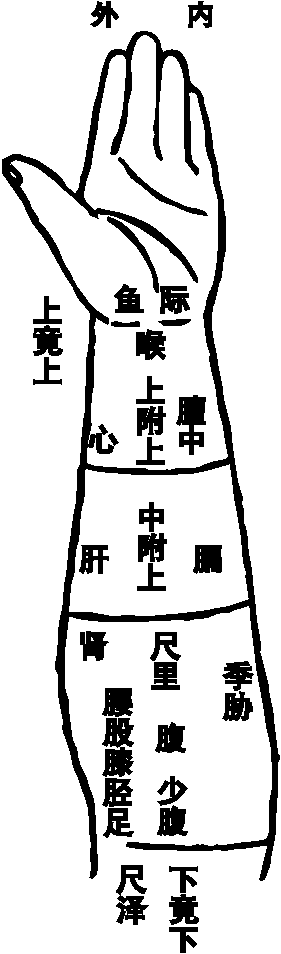
\includegraphics[width=0.14\textwidth]{尺肤切诊部位示意图(左手).pdf}}
	\hspace{3mm}
	\subcaptionbox{右手}
		{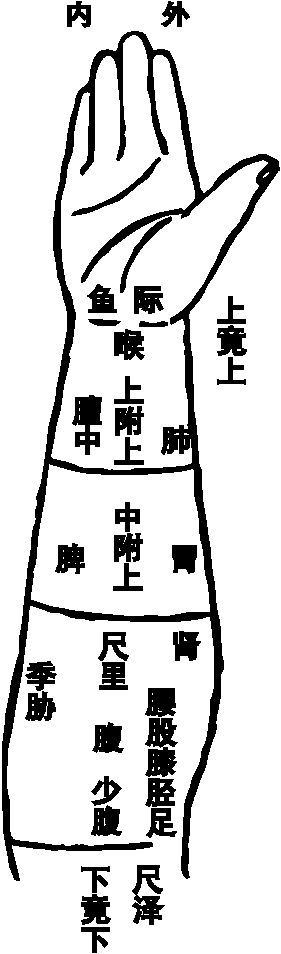
\includegraphics[width=0.14\textwidth]{尺肤切诊部位示意图(右手).pdf}}
	\caption{尺肤切诊部位示意图}
	\label{fig:尺肤切诊部位示意图} %% label for entire figure
\end{wrapfigure}
对“尺内两旁,则季胁也,……少腹腰股膝胫足中事也。”段的注释、理解,有三种观点:一是杨上善、王冰等认为是诊尺肤的脏腑身躯分候部位。(可参图\ref{fig:尺肤切诊部位示意图},详其义。)二是马莳、张介宾等认为是论述以气口寸、关、尺三部脉来诊察脏腑身躯。马莳曰:“后世王叔和之脉,其分部与此大同也欤。”三是认为是指全身诊察法而言,如近人时逸人曰:“《内经》原意系全身诊察法,所谓尺内两旁则季肋也,臂肘湾为尺泽部位,身躯两旁当臂肘湾处,即为季肋。其余则以尺肘部为基础,说明诸脏器邻近之部位,词意非常明显,无庸怀疑。后人误会,硬将全身诊察方法分配于手腕寸关尺三部。”

丹波元简对尺诊之所指作了详细的考察,他在《素问识》中说:“王冰注:‘尺内,谓尺泽之内也。’此即诊尺肤之部位。《平人气象论》云:‘尺涩脉滑,尺寒脉细。’王注亦云‘谓尺肤也’。《邪气脏腑病形》篇云;‘善调尺者,不待于寸。’又云:‘夫色脉与尺之相应,如桴鼓影响之相应也。’《论疾诊尺》篇云‘尺肤泽’,又云‘尺肉弱’。《十三难》云:‘脉数尺之皮肤亦数,脉急尺之皮肤亦急。’《史记·仓公传》亦云:‘切其脉,循其尺。’仲景云‘按寸不及尺’。皆其义也……明是尺即谓臂内一尺之部分,而绝非寸关尺之尺也。寸口分寸关尺三部仿于《难经》,马、张诸家以寸关尺之尺释之,与经旨差矣。”丹波氏之说可从。不过,本段原文虽非论寸口分为寸关尺三部以诊各脏腑,但《难经》关于寸关尺之脏腑划分的观点,其学术渊源显然与本段经旨密切相关,而后世盛行的“左手心肝肾,右手肺脾命”的寸关尺脉象定位说,显然是在本段尺肤诊脏腑定位的启迪下形成的。

\biaoti{【临证指要】}

1.色脉互参的临证意义

色脉互参是四诊合参的重要内容,脉诊可直接诊其内在经脉气血变化,面色是脏腑气血的盛衰和病变反映于外较易诊察者,因此《内经》常用色脉互参的方法诊断疾病,并有诸多的举例,如本段“征其脉小色不夺者,新病也;……征其脉与五色俱不夺者,新病也。”就是色脉互参诊病的一典型范例,以色脉互参的方法,来了解疾病的新久吉凶。

《内经》对于难以把握的真脏脉,也是以色脉互参之法来判断。《素问·玉机真脏论》曰:“真肝脉至,中外急,如循刀刃,责责然,如按琴瑟弦,色青白不泽,毛折乃死。”说明确诊是否肝真脏脉,除了脉诊外还应结合望面部之色,若已有本脏之肝木青色,还见所不胜之肺金白色,及全身衰败的表现,据此可确诊为肝的真脏脉,并可判断其预后凶险。

《难经》对色脉互参亦十分重视,如《难经·十三难》曰:“经言见其色而不得其脉,反得相胜之脉者即死;得相生之脉者病即自已。”,在四诊中,问诊从病人或他人处而得,闻诊主要是闻声、闻气味。在病人不发言语,又无他人提供病情的情况下,只有采取望诊与脉诊,要靠医生充分发挥主观能动性,尽心尽力而得,这也是《内经》屡论色脉互参的意义所在。

2.尺肤诊的临证意义

尺肤诊是《内经》所创立的特有诊病方法,在《内经》切诊中占有重要地位,其内容除散见诸篇外,尚有《灵枢·论疾诊尺》专篇论。诊尺肤主要是诊察尺肤部皮肉的大、小、缓、急、滑、涩及温度的变化,故《灵枢·论疾诊尺》曰:“审其尺之缓急小大滑涩,肉之坚脆而病形定矣。”从临床上来看,可有以下意义。①可判定病位:如本段所言“尺内两旁,则季胁也,……少腹腰股膝胫足中事也。”②可判断病因病性:如《灵枢·论疾诊尺》曰:“尺肤滑,其淖泽者,风也;尺肉弱者,解㑊、安卧;脱肉者,寒热不治;尺肤滑而泽脂者,风也;尺肤涩者,风痹也;尺肤粗如枯鱼之鳞者,水泆饮也。”③尺脉结合,全而认识疾病:·如《灵枢·论疾诊尺》曰:“尺肤热甚,脉盛躁者,病温也,其脉盛而滑者,病且出也。尺肤寒,其脉小者,泄,少气。”“尺炬然热,人迎大者,当夺血。尺坚大,脉小甚,少气,悗有加,立死。”《素问·平人气象论》也有尺脉合参的记载。后世医家对尺肤诊在临床上应用较少,作为切诊方法之一,有待进一步研究。

\section{素問·平人氣象論(節選)}%第二节

\biaoti{【原文】}

\begin{yuanwen}
黃帝問曰:平人何如?岐伯對曰:人一呼脈再動,一吸脈亦再動,呼吸定息\sb{1},脈五動,閏以太息\sb{2},命曰平人。平人者,不病也。常以不病調病人\sb{3},醫不病,故為病人平息以調之為法\sb{4}。

人一呼脈一動,一吸脈一動,曰少氣\sb{5}。人一呼脈三動,一吸脈三動而躁,尺熱曰病温,尺不熱脈滑曰病風,脈濇曰痹\sb{6}。人一呼脈四動以上曰死,脈绝不至曰死,乍踈乍數曰死\sb{7}。
\end{yuanwen}

\biaoti{【校注】}

\begin{jiaozhu}
	\item 呼吸定息:张介宾注:“呼吸定息,谓一息既尽,而换息未起之际也。”
	\item 闰以太息:闰,余也。张志聪注:“太息者,呼吸定息之时,有余不尽而脉又一动,如岁余之有闰也。”
	\item 常以不病调病人:不病,无病健康的人;调(diào),算度、计算、衡量。意为要以健康人(医生)的呼吸来衡量病人的脉息。
	\item 平息以调之为法:平息,即均匀呼吸。调之,衡量病人的脉息至数。吴昆注:“医不病则呼吸调匀,故能为病人平息以调脉。若医者病寒则呼吸迟,病人脉类于数。医者病热则呼吸疾,病人之脉类于迟,皆不足以调病人之脉也。”
	\item 少气:张介宾注:“脉为血气之道路,而脉之运行在乎气,若一呼一吸脉各一动,则一息二至,减少常人之半矣,以正气衰竭也,故曰少气。”
	\item 人一呼脉三动,……脉涩曰痹:尺,指尺肤。濇,同涩。张介宾注:“若不因定息太息而呼吸各三动,是一息六至矣,《难经》谓之离经。躁者,急疾之谓。尺热,言尺中近臂之处有热者,必其通身皆热也。脉数躁而身有热,故知为病温。数滑而尺不热者,阳邪盛也,故当病风;然风之伤人,其变不一,不独在于肌表,故尺不热也。濇为血不调,故当病痹”。
	\item 人一呼脉四动以上曰死,……乍疏乍数曰死:高世栻注:“人一呼脉四动以上,则太过之极。脉绝不至,则不及之极,乍疏乍数,则错乱之极。故皆曰死。”
\end{jiaozhu}

\biaoti{【临证指要】}

\xiaobt{“平息以调之为法”的临证意义}

本段主要论述以脉律来判断平脉、病脉、死脉的诊脉方法,是诊脉的基本要求,一直为后世遵循,沿用至今。

脉理精深微妙,不易掌握,脉象不仅有不易体察的四时权衡规矩沉浮之纲,又有历代二十四、二十八、三十等各家之说,正如陈念祖《医学实在易·八纲脉论》曰:“脉之为道,最为微渺而难知也。方书论脉愈详,而指下愈乱。”故前贤为使习医者切脉辨病能入门执要,提出了当先习知脉之大纲,有谓脉有四纲者,或曰浮、沉、迟、数,或曰迟、数、大、小。有谓脉有六纲者,如周学海《脉简补义·切脉大旨》曰:“《灵枢·邪气脏腑病形》以缓、急、大、小、滑、涩立纲,而以微甚纬之,实开千古诊法之奥,后世有以浮、沉、迟、数分纲者,则其义浅而不备矣。”有谓脉有八纲者,如陈念祖《医学实在易·八纲脉论》指出为浮、沉、迟、数、细、大、短、长。

综观各家之论,不论几脉为纲,其迟、数均为其要,《难经·九难》更认为“数者腑也,迟者脏也。数则为热,迟则为寒。诸阳为热,诸阴为寒,故以别知脏腑之病也。”迟数不仅是辨脏腑寒热阴阳之纲,同时也是易于掌握的,故本篇先论其辨识之法。

\biaoti{【原文】}

\begin{yuanwen}
平人之常氣禀於胃;胃者,平人之常氣也\sb{1}。人無胃氣曰逆,逆者死。春胃微弦曰平\sb{2},弦多胃少曰肝病,但弦無胃曰死\sb{3}。胃而有毛曰秋病,毛甚曰今病\sb{4},藏真散於肝,肝藏筋膜之氣也\sb{5},夏胃微鈎\sb{6}曰平,鈎多胃少曰心病,但钩無胃曰死;胃而有石曰冬病,石甚曰今病,藏真通于心,心藏血脈之氣也。長夏胃微耎弱\sb{7}曰平,弱多胃少曰脾病,但代\sb{8}無胃曰死;耎弱有石曰冬病,弱甚曰今病\sb{9}。藏真濡於脾,脾藏肌肉之氣也。秋胃微毛\sb{10}曰平,毛多胃少曰肺病,但毛無胃曰死;毛而有弦曰春病,弦甚曰今病,藏真高於肺,以行榮衛陰陽也。冬胃微石\sb{11}曰平,石多胃少曰腎病,但石無胃曰死;石而有鈎曰夏病,鈎甚曰今病,藏真下於腎,腎藏骨髓之气也。
\end{yuanwen}

\biaoti{【校注】}

\begin{jiaozhu}
	\item 胃者,平人之常气也:常气,正常人的脉气。意为无病正常人脉象应具有胃气。
	\item 春胃微弦曰平:春季(肝脏)脉有胃气而略带弦,是正常的脉。吴昆注:“弦,脉引而长,若琴弦也。胃,冲和之名。春脉宜弦,必于冲和之中微带弦,是曰平调之脉。”下文“夏胃微钩”、“长夏胃微耎弱”等,义皆同此。
	\item 弦多胃少曰肝病,但弦无胃曰死;吴昆注:“弦多胃少,是肝木偏胜而失其冲和之气,故为肝病。但弦急之脉,更无冲和之气,是失其生道。故死。”下文“钩多胃少”、“弱多胃少”、“但钩无胃”、“但石无胃”等,义皆同此。
	\item 胃而有毛曰秋病,毛甚曰今病:张介宾注:“毛为秋脉属金,春时得之,是谓贼邪,以胃气尚存,故至秋而后病。春脉毛甚,则木被金伤,故不必至秋,今即病矣。”
	\item 脏真散于肝,肝藏筋膜之气:脏真,指五脏所藏的真气。吴昆注:“春时肝木用事,故五脏天真之气,皆散于肝。”肝主筋,故肝藏筋膜之气。下文“通于心”、“濡于脾”、“高于肺”、“下于肾”义皆仿此。高世栻注:“盖肝主疏泄,故曰散。心主血脉,故曰通。脾主灌溉,故曰濡。肺位居上,故曰高。肾为水脏,故曰下也。”
	\item 钩:夏季主脉,即洪大脉,如钩端微曲之象。
	\item 耎弱:耎,同软。耎弱,指柔和而不劲急的脉象,为脾脏主脉。
	\item 代:其义有两说,一是谓弱极,如高世栻注:“代,软弱之极也。软弱极而无胃气,则曰死脉。”一是谓更代,如张介宾注:“代,更代也。脾主四季,脉当随时而更,然必欲皆兼和耎,方得脾脉之平。若四季相代,而但弦、但钩、但毛、但石,是但代无胃,现真脏也,故曰死。”
	\item 耎弱有石曰冬病,弱甚曰今病:弱甚,《甲乙经·卷四》、《千金要方·卷十五》均作“石甚”。张介宾注:“石为冬脉属水,长夏阳气正盛而见沉石之脉,以火土气衰,而水反乘也,故至冬而病。弱,当作石。长夏石甚者,火土大衰,故不必至冬,今即病矣。”
	\item 毛:秋季主脉,似浮脉。王冰注:“谓如物之浮,如风吹毛也。”
	\item 石:冬季主脉,脉来沉而实,如石沉水中。
\end{jiaozhu}

\biaoti{【理论阐释】}

\xiaobt{脉以胃气为本}

辨五脏之脉的平脉、病脉、死脉以及兼脉,主要是据脉中的“胃气”。所谓“胃气”不仅指胃本身具有的受纳、腐熟、和降等功能,而且还包含胃腑机能在整个机体中的作用,故“胃气”与人的生命息息相关,正如本篇说:“人以水谷为本,故人绝水谷则死,脉无胃气亦死。”又说:“平人之常气禀于胃,胃者,平人之常气也,人无胃气曰逆,逆者死。”

脉以胃气为本,其理如下:①脉气根源于五脏六腑,胃为之本。《素问·调经论》曰:“五脏之道,皆出于经隧,以行血气。”五脏功能活动依赖于胃气,正如《素问·玉机真脏论》所说:“五脏者,皆禀气于胃,胃者五脏之本也。”②脉中血气源于水谷之气。《灵枢·本脏》曰:“经脉者,所以行血气而营阴阳……是故血和则经脉流行。”人生理活动所需要的各种精气均由水谷之气所化,如《灵枢·决气》论述了六气(精、气、血、津、液、脉)由一气(水谷之气)而化,最后又强调曰:“六气者然五谷与胃为大海。”③肺气附于胃气,推动脉气运行。“诸气者皆属于肺”,脉气亦离不开肺气之助,然肺气能行血脉之中,常依附于胃化生的水谷之气,如《灵枢·动输》曰:“胃为五脏六腑之海,其清气上注于肺,肺气从太阴而行之。其行也以息往来,故人一呼脉再动,一吸脉亦再动,呼吸不已,故动而不止。”④胃气运脏真之气于脉中。脏真之气是五脏之先天真气,然其必依赖胃气才能行于经脉之中,在全身发挥其应有的功能,所以《素问·玉机真脏论》说:“脏气者,不能自致于手太阴,必因于胃气,乃至于手太阴也。”

由于经脉的正常活动依赖胃气,所以五脏应时之气与饱满的胃气相合,表现于脉中,才是五脏康健之正常脉象,若胃气不足则为五脏病脉,只有应时之脉而无胃气,则为毫无生机的五脏死脉,又称真脏脉。

\biaoti{【临证指要】}

\xiaobt{脉以胃气为本的临床意义}

《内经》脉以胃气为本的观点,对后世脉学的发展具有十分重要的影响,并且为后世临床重视胃气,尤其对治疗重病危症更需顾护胃气,以及脾为后天之本理论的提出,均具有指导意义。

何谓脉有胃气,《素问·玉机真脏论》曰:“脉弱以滑,是有胃气。”此处之“弱”是柔和之意,滑指脉来流利。《灵枢·终始》曰:“谷气来也徐而和。”此处的“谷气”即指脉之胃气。故张介宾曰:“自有一种雍容和缓之状者,便是有胃气之脉。”因此可以说,凡脉来和缓均匀、不浮不沉、不大不小、不疾不徐、不长不短,应手柔和有力、来去节律整齐,有生机勃勃之象的脉,便是有胃气之脉。历代医家对胃脉的形态以及临床应用多有阐发,使诊察脉象有无胃气成为临床预后疾病的重要内容。如张介宾《景岳全书·胃气解》曰:“察之之法,如今日尚和缓,明日更弦急,知邪气之愈进,邪愈进则病愈甚矣;今日甚弦急,明日稍和缓,知胃气之渐至,胃气至则病渐轻矣。即如顷刻之间,初急后缓者,胃气之来也;初缓后急者,胃气之去也,此察邪正进退之法也。至于生死之兆,亦唯以胃气为主。”当今中医认为平人之脉不但要有“胃气”,而且还要具备“有神”、“有根”的特点。实际上脉的神、根仍然是在“脉以胃气为本”的基础上发展起来的。

“以胃气为本”的理论还应用到其他诊法之中,如胃气是舌苔形成的基础,故望舌苔以判断胃气的盛衰、邪气的进退。在问诊方面,若粥架不入,知其胃气衰败,预后不良等。

\biaoti{【原文】}

\begin{yuanwen}
胃之大絡,名曰虚里\sb{1},贯鬲絡肺,出於左乳下,其動應衣,脈宗氣也\sb{2}。盛喘數絕者,則病在中\sb{2};結而横,有積矣\sb{4};絕不至,日死。乳之下,其動應衣,宗气泄也\sb{5}。
\end{yuanwen}

\biaoti{【校注】}

\begin{jiaozhu}
	\item 虚里:是足阳明胃经除丰隆外的又一大的络脉,其脉从胃贯穿膈膜络于肺,出于左乳下。后世亦将心尖搏动处,谓之虚里。
	\item 其动应衣,脉宗气也:衣,《甲乙经》作“手”。脉,动词,诊察的意思。一说,“脉宗气”,作“脉气之宗解”。可参。
	\item 盛喘数绝者,则病在中:盛喘,指虚里处搏动之甚如气急之喘促;数,屡次之意;绝,断绝,指搏动停止。张介宾注:“若虚里动甚而如喘,或数急而兼断绝者,由中气不守而言,故曰病在中。”
	\item 结而横,有积矣:结,脉来迟,时一止;横,有充满、坚硬之意;积,指积聚之证。
	\item 乳之下,其动应衣,宗气泄也:吴昆注:“宗气宜藏不宜泄,乳下虚里之脉,其动应衣,是宗气失藏而外泄也。”
\end{jiaozhu}

\biaoti{【临证指要】}

\xiaobt{虚里诊法的临床价值}

经文举例说明了虚里诊四种情况:①虚里搏动“盛喘数绝”,反映体中的胃及心肺有疾;②虚里搏动“结而横”说明内有积聚;③若虚里搏动“绝不至”(跳动中断,绝而不复),预后不良;④搏动剧烈,“其动应衣”,是宗气大泄之证,预后亦差。经文虽然简短,但颇被后世医家重视,如魏柳洲曰:“凡治小儿,不论诸证,宜先揣虚里穴,若跳甚者,不可攻伐,以其先天不足故也。”王士雄曰:“小儿则脉候难凭,揣此尤为可据。”此外,临证如遇暴厥、大虚大实脉伏不见之证,亦可应用虚里诊法,协助诊断。尽管这一古老的诊断方法在目前中医诊断学上很少提及,但其在临床上的价值是不能忽视的。

\biaoti{【原文】}

\begin{yuanwen}
頸脈動喘疾欬\sb{1},曰水。目裹微腫,如卧蠶起之狀\sb{2},曰水。溺黄赤安卧者,黄疸\sb{3}。已食如飢者,胃疸\sb{4}。面腫曰風,足脛腫曰水。目黄者曰黄疸。婦人手少陰脈\sb{5}動甚者,妊子也。

脈有逆從四時,未有藏形\sb{6},春夏而脈瘦\sb{7},秋冬而脈浮大,命曰逆四時也。風熱而脈靜,泄而脱血脈實,病在中脈虚,病在外脈濇堅者,皆難治,命曰反四時也\sb{8}。
\end{yuanwen}

\biaoti{【校注】}

\begin{jiaozhu}
	\item 颈脉动喘疾咳:颈脉,即人迎脉,属足阳明胃经。张介宾注:“水气上逆,反侵阳明则颈脉动。水溢于肺,则喘急而疾咳。”
	\item 目裹微肿,如卧蚕起之状:张介宾注:“目裹者,目下之胞也,胃脉之所至,脾气之所主,若见微肿如卧蚕起之状,是水气淫及脾胃也。”
	\item 黄疸:病证名,多由湿热或寒湿内阻中焦所致。
	\item 胃疸:疸,与瘅通,热也。王冰注:“是则冒热也,热则消谷,故食己如饥也。”
	\item 手少阴脉;指神门穴部位之脉。王冰注:“手少阴脉,谓掌后陷者中,当小指动而应手者也。”
	\item 未有脏形:脏形,即五脏应四时的正常脉象。未有脏形,是指不见本脏应时的脉象。
	\item 脉瘦:指沉细脉象。
	\item 风热而脉静,……命曰反四时也:马莳注:“此言脉与病反者,是亦脉与时反之意也。病由风热,脉宜浮大而反沉静,则阳病见阴脉也。泄利脱血二证,脉宜沉细而反实大,则阴病见阳脉也。病在中者,脉为有力,则中气方盛,今脉反虚;病在外者,脉宜浮虚,则表病易痊,今脉反涩坚,是皆难治之证,犹脉之反四时也。”
\end{jiaozhu}

\biaoti{【理论阐释】}

\xiaobt{妊娠脉的诊断}

本段提到了妊娠脉的诊断“妇人手少阴脉动甚者,妊子也。”与《灵枢·论疾诊尺》中“女子手少阴脉动甚者妊子”同,手少阴究竟何指,历代注家意见不一。①王冰谓手少阴神门穴处的搏动。②张志聪、高世栻认为是两手寸口脉的尺部,如高氏曰:“少阴,尺脉也……两手少阴脉动甚者,则知肾气有余,感天一所生之气,故妊子也。”③马莳认为是左手寸口的寸部。注曰:“左手寸部属手少阴心经……故知手少阴之脉动甚者,为妊男子也。”④认为“手少阴”当作“足少阴”。如《新校正》云:“按全元起本作足少阴。”

验之临床,高氏、张氏意见可从,这与《素问·阴阳别论》所说的“阴搏阳别,谓之有子”的精神一致。关前为阳以候心,关后为阴以候肾。一般认为尺部脉象滑利有力是妊娠的脉候。但按神门穴在临床上也有应用。如张志聪“左手少阴肾脉动甚者,当妊子,以左男而右女”的说法,亦为目前少数医者所认同。

总之,以脉辨妊娠在临床上有其一定价值。因为妊娠期间机体有效循环血量显著增加,超过正常血液总量的33\%以上,此时心脏的收缩力量显著加强,每次搏出量增加,因而脉搏就相应地有力流畅,尽管脉象的形成受多种因素影响,但有效循环血量和心脏收缩力毕竟起着重要的作用,可见,古人凭脉辨妊娠的方法有其一定生理基础。当然在运用这一诊脉方法时,还需结合其月经史以及有关情况,才能做出准确的判断。

\section{靈樞·五色(節選)}%第三節

\biaoti{【原文】}

\begin{yuanwen}
雷公曰:五官之辨奈何?黃帝曰:明堂骨高以起,平以直\sb{1},五藏次於中央,六府挾其兩側\sb{2},首面上於闕庭\sb{3},王宫在於下極\sb{4},五藏安於胸中\sb{5},真色以致\sb{6},病色不見,明堂潤澤以清\sb{7},五官惡\sb{8}得無辨乎……

沉濁為內,浮澤為外\sb{9},黃赤為風,青黑為痛,白為寒\sb{10},黃而膏潤為膿,赤甚者為血\sb{11},痛甚為攣,寒甚為皮不仁\sb{12}。五色各見其部,察其浮沉,以知淺深\sb{13};察其澤夭,以觀成敗\sb{14};察其散搏,以知遠近\sb{15};視色上下,以知病處\sb{16};積神於心,以知往今\sb{17}。
\end{yuanwen}

\biaoti{【校注】}

\begin{jiaozhu}
	\item 明堂骨高以起,平以直:明堂,本指古时帝王宣明政教之处,此指鼻部。意为鼻骨高隆起,平正而端直。
	\item 五脏次于中央,六腑挟其两侧:五脏所主部位依此排列在面部的中央,六腑所主部位则挟于其两旁。
	\item 首面上于阙庭;阏,宫门外两侧的楼台,中间有道路,其处置门,谓之阙门,本篇以阙门比喻两眉间:庭,堂阶前的地坪,本篇以庭比喻前额部。意为头面部各组织器官的情况向上反映于两眉之间和前额。
	\item 王宫在于下极:王宫,帝王的宫室,此指心脏;下极,即两目之间。意为心脏的情况反映于两目之间的部位。
	\item 胸中:胸腹之中。
	\item 真色以致:真色,正色,为脏腑和调,精气充盈的表现;致,到达、表达。意为正色显现于面部。
	\item 清:清纯、洁净,不污浊。
	\item 恶:怎么,表示反对。
	\item 沉浊为内,浮泽为外:面色沉滞晦浊的为病在里,浮润光泽的为病在表。
	\item 黄赤为风,青黑为痛,白为寒:面色见黄赤的多属逢热一类疾病;青黑色多为血气凝滞,故属疼痛一类的疾病;白色多为寒病。
	\item 黄而膏润为脓,赤甚者为血:此指疮疡而言。
	\item 痛甚为挛,寒甚为皮不仁:不仁,皮肉不知痛痒,感觉迟钝。面色青黑主痛证,而青黑过重主拘挛;面色白主寒证,白色太重主皮肤不仁。
	\item 察其浮沉,以知浅深:色浮者主病浅,色沉者主病深。
	\item 察其夭泽,以观成败:据面色的夭枯与润泽判断预后。
	\item 察其散抟,以知远近:抟,凝聚。病色散而不聚的为病程短暂;病色聚面不散的为病久远。
	\item 视色上下,以知病处:察病色在面部上下脏腑肢节所应的部位,则可了解疾病所在之处。
	\item 积神于心,以知往今:医生察面色时应聚精会神、专心致志,这样才可了解疾病的发展变化。
\end{jiaozhu}

\biaoti{【理论阐解】}

\xiaobt{望面色诊病之理}

人有五脏现五色,以面部表现最为明显,故望面色是望诊的重要内容,面望面色主要是观察病人面部的色泽及异常之色所出现的部位。

本篇以整体观为指导,详细地叙述了五脏六腑,四肢关节在面部相应的望色部位,指出“五脏次于中央,六腑挟共两侧”,“五色之见也各出其色部”。《灵枢·邪气脏腑病形》也曰:“十二经脉,三百六十五络,其血气皆上于面”。正是由于经脉气血的联系,面部可为全身脏腑肢节的缩影,故可以反映脏腑肢节的病理变化。

这种以局部为整体一个缩影的论述,与现代生物全息思想有相通之处。根据生物全息律的一般原理,人体的任何一相对独立的部位,如每一肢节,每一器官,也应寓藏着整个机体的生命信息。从信息角度而言,也可以说经络是一人体信息的通道,气血是信息的载体,十二经脉之气血皆上于面,将整体的信息传输于面部,使面部成为全身的缩影,因而通过面部不同部位的色泽变化可以诊断全身疾病。

\biaoti{【临证指要】}

\xiaobt{察面色的临床运用}

临床上诊察面色测知疾病,有以下几个方面。①察色要做到全神贯注,细心观察,诊断才能正确。②从面部病色出现与脏腑肢节相应的部位,诊知疾病所在。③察色浮沉,可辨病位的表里深浅。④察五色不同,可辨病因,定病性,即“黄赤为风,青黑为痛,白为寒。”⑤可判定一些病症,如“黄而膏润为脓,赤甚者为血”,“病甚为挛,寒甚为皮不仁。”⑥察色散抟,辨别病程长短“远近”。⑦察色清浊,测知病情的轻重。⑧察色夭泽,辨病吉凶,这些与《素问·脉要精微论》所论五欲、五不欲的精神是一致的。

后世医家在运用《内经》理论基础上又各从不同方面有所发展。如清·汪宏《望诊遵经》提出望浮沉、清浊、微甚、散抟,泽夭十法,用以鉴别疾病的表里、阴阳、虚实、新久、轻重。若将面色各部综合运用,更能辨病入微。如眼黑为痰饮中停,颧红为火热内盛,故眼黑颧红则主痰热等。

\xiaojie

本章所选经文篇章虽不多,但已涉及到诊法诸方面的内容。

1.对诊法的要求,提出了“虚静为保”、“诊法常以平旦”等,其精神实质为诊病是一个十分慎重的事情,要环境相对安静、病人心情安稳,医生更应专心致志。这不仅是准确获得病情的基础,也反映出医德医风之渊源。

2.应多诊合参,对望诊、切诊合参论述较多,如色脉合参,寸尺合参等。后世遵其理,提出了四诊合参,以求病本,使中医诊断更具特色。

3.切诊尤其脉诊是本章的主要内容:①脉诊可以诊断全身的气血盛衰。诊脉的方法,是“常以不病调病人”、“平息以调之为法”。②论述了脉应四时,提示诊脉要注意天人相应的关系。③脉以胃气为本,据胃气的有无多少判断平脉、病脉、死脉,无胃气的脉,就是死脉,又称真脏脉。这种重视胃气的思想,不仅对后世的脉学有着深刻的影响,而且对中医理论的发展以及临床治疗等方面都有十分重要的指导意义。④尺肤和虚里的诊断方法及诊断意义。⑤脉有逆从阴阳的论述,对疾病的预后有着重要意义,亦说明了疾病的复杂性,临床需辨真伪,由此后世提出了舍脉从证,舍证从脉等权变之法。

4.关于望诊,本章论述了望眼神、望面色以及望形态。对望面色的意义、临床应用进行了说明,对望面色的要点阐述详明。为望诊的发展奠定了基础。

5.对问诊、闻诊本章也有一定的论述,如“声如从室中言”、“水泉不止”、释梦诊病等,皆是闻诊和问诊的内容。

\zuozhe{(周发祥)}
\ifx \allfiles \undefined
\end{document}
\fi    % 第六章 诊法
% -*- coding: utf-8 -*-
%!TEX program = xelatex
\ifx\allfiles\undefined
\documentclass[draft,12pt]{ctexbook}
%\usepackage{xeCJK}
%\usepackage[14pt]{extsizes} %支持8,9,10,11,12,14,17,20pt

%===================文档页面设置====================
%---------------------印刷版尺寸--------------------
%\usepackage[a4paper,hmargin={2.3cm,1.7cm},vmargin=2.3cm,driver=xetex]{geometry}
%--------------------电子版------------------------
\usepackage[a4paper,margin=2cm,driver=xetex]{geometry}
%\usepackage[paperwidth=9.2cm, paperheight=12.4cm, width=9cm, height=12cm,top=0.2cm,
%            bottom=0.4cm,left=0.2cm,right=0.2cm,foot=0cm, nohead,nofoot,driver=xetex]{geometry}

%===================自定义颜色=====================
\usepackage{xcolor}
  \definecolor{mybackgroundcolor}{cmyk}{0.03,0.03,0.18,0}
  \definecolor{myblue}{rgb}{0,0.2,0.6}

%====================字体设置======================
%--------------------中文字体----------------------
%-----------------------xeCJK下设置中文字体------------------------------%
\setCJKfamilyfont{song}{SimSun}                             %宋体 song
\newcommand{\song}{\CJKfamily{song}}                        % 宋体   (Windows自带simsun.ttf)
\setCJKfamilyfont{xs}{NSimSun}                              %新宋体 xs
\newcommand{\xs}{\CJKfamily{xs}}
\setCJKfamilyfont{fs}{FangSong_GB2312}                      %仿宋2312 fs
\newcommand{\fs}{\CJKfamily{fs}}                            %仿宋体 (Windows自带simfs.ttf)
\setCJKfamilyfont{kai}{KaiTi_GB2312}                        %楷体2312  kai
\newcommand{\kai}{\CJKfamily{kai}}
\setCJKfamilyfont{yh}{Microsoft YaHei}                    %微软雅黑 yh
\newcommand{\yh}{\CJKfamily{yh}}
\setCJKfamilyfont{hei}{SimHei}                                    %黑体  hei
\newcommand{\hei}{\CJKfamily{hei}}                          % 黑体   (Windows自带simhei.ttf)
\setCJKfamilyfont{msunicode}{Arial Unicode MS}            %Arial Unicode MS: msunicode
\newcommand{\msunicode}{\CJKfamily{msunicode}}
\setCJKfamilyfont{li}{LiSu}                                            %隶书  li
\newcommand{\li}{\CJKfamily{li}}
\setCJKfamilyfont{yy}{YouYuan}                             %幼圆  yy
\newcommand{\yy}{\CJKfamily{yy}}
\setCJKfamilyfont{xm}{MingLiU}                                        %细明体  xm
\newcommand{\xm}{\CJKfamily{xm}}
\setCJKfamilyfont{xxm}{PMingLiU}                             %新细明体  xxm
\newcommand{\xxm}{\CJKfamily{xxm}}

\setCJKfamilyfont{hwsong}{STSong}                            %华文宋体  hwsong
\newcommand{\hwsong}{\CJKfamily{hwsong}}
\setCJKfamilyfont{hwzs}{STZhongsong}                        %华文中宋  hwzs
\newcommand{\hwzs}{\CJKfamily{hwzs}}
\setCJKfamilyfont{hwfs}{STFangsong}                            %华文仿宋  hwfs
\newcommand{\hwfs}{\CJKfamily{hwfs}}
\setCJKfamilyfont{hwxh}{STXihei}                                %华文细黑  hwxh
\newcommand{\hwxh}{\CJKfamily{hwxh}}
\setCJKfamilyfont{hwl}{STLiti}                                        %华文隶书  hwl
\newcommand{\hwl}{\CJKfamily{hwl}}
\setCJKfamilyfont{hwxw}{STXinwei}                                %华文新魏  hwxw
\newcommand{\hwxw}{\CJKfamily{hwxw}}
\setCJKfamilyfont{hwk}{STKaiti}                                    %华文楷体  hwk
\newcommand{\hwk}{\CJKfamily{hwk}}
\setCJKfamilyfont{hwxk}{STXingkai}                            %华文行楷  hwxk
\newcommand{\hwxk}{\CJKfamily{hwxk}}
\setCJKfamilyfont{hwcy}{STCaiyun}                                 %华文彩云 hwcy
\newcommand{\hwcy}{\CJKfamily{hwcy}}
\setCJKfamilyfont{hwhp}{STHupo}                                 %华文琥珀   hwhp
\newcommand{\hwhp}{\CJKfamily{hwhp}}

\setCJKfamilyfont{fzsong}{Simsun (Founder Extended)}     %方正宋体超大字符集   fzsong
\newcommand{\fzsong}{\CJKfamily{fzsong}}
\setCJKfamilyfont{fzyao}{FZYaoTi}                                    %方正姚体  fzy
\newcommand{\fzyao}{\CJKfamily{fzyao}}
\setCJKfamilyfont{fzshu}{FZShuTi}                                    %方正舒体 fzshu
\newcommand{\fzshu}{\CJKfamily{fzshu}}

\setCJKfamilyfont{asong}{Adobe Song Std}                        %Adobe 宋体  asong
\newcommand{\asong}{\CJKfamily{asong}}
\setCJKfamilyfont{ahei}{Adobe Heiti Std}                            %Adobe 黑体  ahei
\newcommand{\ahei}{\CJKfamily{ahei}}
\setCJKfamilyfont{akai}{Adobe Kaiti Std}                            %Adobe 楷体  akai
\newcommand{\akai}{\CJKfamily{akai}}

%------------------------------设置字体大小------------------------%
\newcommand{\chuhao}{\fontsize{42pt}{\baselineskip}\selectfont}     %初号
\newcommand{\xiaochuhao}{\fontsize{36pt}{\baselineskip}\selectfont} %小初号
\newcommand{\yihao}{\fontsize{28pt}{\baselineskip}\selectfont}      %一号
\newcommand{\xiaoyihao}{\fontsize{24pt}{\baselineskip}\selectfont}
\newcommand{\erhao}{\fontsize{21pt}{\baselineskip}\selectfont}      %二号
\newcommand{\xiaoerhao}{\fontsize{18pt}{\baselineskip}\selectfont}  %小二号
\newcommand{\sanhao}{\fontsize{15.75pt}{\baselineskip}\selectfont}  %三号
\newcommand{\sihao}{\fontsize{14pt}{\baselineskip}\selectfont}%     四号
\newcommand{\xiaosihao}{\fontsize{12pt}{\baselineskip}\selectfont}  %小四号
\newcommand{\wuhao}{\fontsize{10.5pt}{\baselineskip}\selectfont}    %五号
\newcommand{\xiaowuhao}{\fontsize{9pt}{\baselineskip}\selectfont}   %小五号
\newcommand{\liuhao}{\fontsize{7.875pt}{\baselineskip}\selectfont}  %六号
\newcommand{\qihao}{\fontsize{5.25pt}{\baselineskip}\selectfont}    %七号   %中文字体及字号设置
\xeCJKDeclareSubCJKBlock{SIP}{
  "20000 -> "2A6DF,   % CJK Unified Ideographs Extension B
  "2A700 -> "2B73F,   % CJK Unified Ideographs Extension C
  "2B740 -> "2B81F    % CJK Unified Ideographs Extension D
}
%\setCJKmainfont[SIP={[AutoFakeBold=1.8,Color=red]Sun-ExtB},BoldFont=黑体]{宋体}    % 衬线字体 缺省中文字体

\setCJKmainfont{simsun.ttc}[
  Path=fonts/,
  SIP={[Path=fonts/,AutoFakeBold=1.8,Color=red]simsunb.ttf},
  BoldFont=simhei.ttf
]

%SimSun-ExtB
%Sun-ExtB
%AutoFakeBold:自动伪粗,即正文使用\bfseries时生僻字使用伪粗体;
%FakeBold:强制伪粗,即正文中生僻字均使用伪粗体
%\setCJKmainfont[BoldFont=STHeiti,ItalicFont=STKaiti]{STSong}
%\setCJKsansfont{微软雅黑}黑体
%\setCJKsansfont[BoldFont=STHeiti]{STXihei} %serif是有衬线字体sans serif 无衬线字体
%\setCJKmonofont{STFangsong}    %中文等宽字体

%--------------------英文字体----------------------
\setmainfont{simsun.ttc}[
  Path=fonts/,
  BoldFont=simhei.ttf
]
%\setmainfont[BoldFont=黑体]{宋体}  %缺省英文字体
%\setsansfont
%\setmonofont

%===================目录分栏设置====================
\usepackage[toc,lof,lot]{multitoc}    % 目录(含目录、表格目录、插图目录)分栏设置
  %\renewcommand*{\multicolumntoc}{3} % toc分栏数设置,默认为两栏(\multicolumnlof,\multicolumnlot)
  %\setlength{\columnsep}{1.5cm}      % 调整分栏间距
  \setlength{\columnseprule}{0.2pt}   % 调整分栏竖线的宽度

%==================章节格式设置====================
\setcounter{secnumdepth}{3} % 章节等编号深度 3:子子节\subsubsection
\setcounter{tocdepth}{2}    % 目录显示等度 2:子节

\xeCJKsetup{%
  CJKecglue=\hspace{0.15em},      % 调整中英(含数字)间的字间距
  %CJKmath=true,                  % 在数学环境中直接输出汉字(不需要\text{})
  AllowBreakBetweenPuncts=true,   % 允许标点中间断行,减少文字行溢出
}

\ctexset{%
  part={
    name={,篇},
    number=\SZX{part},
    format={\chuhao\bfseries\centering},
    nameformat={},titleformat={}
  },
  section={
    number={\chinese{section}},
    name={第,节}
  },
  subsection={
    number={\chinese{subsection}、},
    aftername={\hspace{-0.01em}}
  },
  subsubsection={
    number={(\chinese{subsubsection})},
    aftername={\hspace {-0.01em}},
    beforeskip={1.3ex minus .8ex},
    afterskip={1ex minus .6ex},
    indent={\parindent}
  },
  paragraph={
    beforeskip=.1\baselineskip,
    indent={\parindent}
  }
}

\newcommand*\SZX[1]{%
  \ifcase\value{#1}%
    \or 上%
    \or 中%
    \or 下%
  \fi
}

%====================页眉设置======================
\usepackage{titleps}%或者\usepackage{titlesec},titlesec包含titleps
\newpagestyle{special}[\small\sffamily]{
  %\setheadrule{.1pt}
  \headrule
  \sethead[\usepage][][\chaptertitle]
  {\chaptertitle}{}{\usepage}
}

\newpagestyle{main}[\small\sffamily]{
  \headrule
  %\sethead[\usepage][][第\thechapter 章\quad\chaptertitle]
%  {\thesection\quad\sectiontitle}{}{\usepage}}
  \sethead[\usepage][][第\chinese{chapter}章\quad\chaptertitle]
  {第\chinese{section}节\quad\sectiontitle}{}{\usepage}
}

\newpagestyle{main2}[\small\sffamily]{
  \headrule
  \sethead[\usepage][][第\chinese{chapter}章\quad\chaptertitle]
  {第\chinese{section}節\quad\sectiontitle}{}{\usepage}
}

%================ PDF 书签设置=====================
\usepackage{bookmark}[
  depth=2,        % 书签深度 2:子节
  open,           % 默认展开书签
  openlevel=2,    % 展开书签深度 2:子节
  numbered,       % 显示编号
  atend,
]
  % 相比hyperref,bookmark宏包大多数时候只需要编译一次,
  % 而且书签的颜色和字体也可以定制。
  % 比hyperref 更专业 (自动加载hyperref)

%\bookmarksetup{italic,bold,color=blue} % 书签字体斜体/粗体/颜色设置

%------------重置每篇章计数器,必须在hyperref/bookmark之后------------
\makeatletter
  \@addtoreset{chapter}{part}
\makeatother

%------------hyperref 超链接设置------------------------
\hypersetup{%
  pdfencoding=auto,   % 解决新版ctex,引起hyperref UTF-16预警
  colorlinks=true,    % 注释掉此项则交叉引用为彩色边框true/false
  pdfborder=001,      % 注释掉此项则交叉引用为彩色边框
  citecolor=teal,
  linkcolor=myblue,
  urlcolor=black,
  %psdextra,          % 配合使用bookmark宏包,可以直接在pdf 书签中显示数学公式
}

%------------PDF 属性设置------------------------------
\hypersetup{%
  pdfkeywords={黄帝内经,内经,内经讲义,21世纪课程教材},    % 关键词
  %pdfsubject={latex},        % 主题
  pdfauthor={主编:王洪图},   % 作者
  pdftitle={内经讲义},        % 标题
  %pdfcreator={texlive2011}   % pdf创建器
}

%------------PDF 加密----------------------------------
%仅适用于xelatex引擎 基于xdvipdfmx
%\special{pdf:encrypt ownerpw (abc) userpw (xyz) length 128 perm 2052}

%仅适用于pdflatex引擎
%\usepackage[owner=Donald,user=Knuth,print=false]{pdfcrypt}

%其他可使用第三方工具 如:pdftk
%pdftk inputfile.pdf output outputfile.pdf encrypt_128bit owner_pw yourownerpw user_pw youruserpw

%=============自定义环境、列表及列表设置================
% 标题
\def\biaoti#1{\vspace{1.7ex plus 3ex minus .2ex}{\bfseries #1}}%\noindent\hei
% 小标题
\def\xiaobt#1{{\bfseries #1}}
% 小结
\def\xiaojie {\vspace{1.8ex plus .3ex minus .3ex}\centerline{\large\bfseries 小\ \ 结}\vspace{.1\baselineskip}}
% 作者
\def\zuozhe#1{\rightline{\bfseries #1}}

\newcounter{yuanwen}    % 新计数器 yuanwen
\newcounter{jiaozhu}    % 新计数器 jiaozhu

\newenvironment{yuanwen}[2][【原文】]{%
  %\biaoti{#1}\par
  \stepcounter{yuanwen}   % 计数器 yuanwen+1
  \bfseries #2}
  {}

\usepackage{enumitem}
\newenvironment{jiaozhu}[1][【校注】]{%
  %\biaoti{#1}\par
  \stepcounter{jiaozhu}   % 计数器 jiaozhu+1
  \begin{enumerate}[%
    label=\mylabel{\arabic*}{\circledctr*},before=\small,fullwidth,%
    itemindent=\parindent,listparindent=\parindent,%labelsep=-1pt,%labelwidth=0em,
    itemsep=0pt,topsep=0pt,partopsep=0pt,parsep=0pt
  ]}
  {\end{enumerate}}

%===================注解与原文相互跳转====================
%----------------第1部分 设置相互跳转锚点-----------------
\makeatletter
  \protected\def\mylabel#1#2{% 注解-->原文
    \hyperlink{back:\theyuanwen:#1}{\Hy@raisedlink{\hypertarget{\thejiaozhu:#1}{}}#2}}

  \protected\def\myref#1#2{% 原文-->注解
    \hyperlink{\theyuanwen:#1}{\Hy@raisedlink{\hypertarget{back:\theyuanwen:#1}{}}#2}}
  %此处\theyuanwen:#1实际指thejiaozhu:#1,只是\thejiaozhu计数器还没更新,故使用\theyuanwen计数器代替
\makeatother

\protected\def\myjzref#1{% 脚注中的引用(引用到原文)
  \hyperlink{\theyuanwen:#1}{\circlednum{#1}}}

\def\sb#1{\myref{#1}{\textsuperscript{\circlednum{#1}}}}    % 带圈数字上标

%----------------第2部分 调整锚点垂直距离-----------------
\def\HyperRaiseLinkDefault{.8\baselineskip} %调整锚点垂直距离
%\let\oldhypertarget\hypertarget
%\makeatletter
%  \def\hypertarget#1#2{\Hy@raisedlink{\oldhypertarget{#1}{#2}}}
%\makeatother

%====================带圈数字列表标头====================
\newfontfamily\circledfont[Path = fonts/]{meiryo.ttc}  % 日文字体,明瞭体
%\newfontfamily\circledfont{Meiryo}  % 日文字体,明瞭体

\protected\def\circlednum#1{{\makexeCJKinactive\circledfont\textcircled{#1}}}

\newcommand*\circledctr[1]{%
  \expandafter\circlednum\expandafter{\number\value{#1}}}
\AddEnumerateCounter*\circledctr\circlednum{1}

% 参考自:http://bbs.ctex.org/forum.php?mod=redirect&goto=findpost&ptid=78709&pid=460496&fromuid=40353

%======================插图/tikz图========================
\usepackage{graphicx,subcaption,wrapfig}    % 图,subcaption含子图功能代替subfig,图文混排
  \graphicspath{{img/}}                     % 设置图片文件路径

\def\pgfsysdriver{pgfsys-xetex.def}         % 设置tikz的驱动引擎
\usepackage{tikz}
  \usetikzlibrary{calc,decorations.text,arrows,positioning}

%---------设置tikz图片默认格式(字号、行间距、单元格高度)-------
\let\oldtikzpicture\tikzpicture
\renewcommand{\tikzpicture}{%
  \small
  \renewcommand{\baselinestretch}{0.2}
  \linespread{0.2}
  \oldtikzpicture
}

%=========================表格相关===============================
\usepackage{%
  multirow,                   % 单元格纵向合并
  array,makecell,longtable,   % 表格功能加强,tabu的依赖
  tabu-last-fix,              % "强大的表格工具" 本地修复版
  diagbox,                    % 表头斜线
  threeparttable,             % 表格内脚注(需打补丁支持tabu,longtabu)
}

%----------给threeparttable打补丁用于tabu,longtabu--------------
%解决方案来自:http://bbs.ctex.org/forum.php?mod=redirect&goto=findpost&ptid=80318&pid=467217&fromuid=40353
\usepackage{xpatch}

\makeatletter
  \chardef\TPT@@@asteriskcatcode=\catcode`*
  \catcode`*=11
  \xpatchcmd{\threeparttable}
    {\TPT@hookin{tabular}}
    {\TPT@hookin{tabular}\TPT@hookin{tabu}}
    {}{}
  \catcode`*=\TPT@@@asteriskcatcode
\makeatother

%------------设置表格默认格式(字号、行间距、单元格高度)------------
\let\oldtabular\tabular
\renewcommand{\tabular}{%
  \renewcommand\baselinestretch{0.9}\small    % 设置行间距和字号
  \renewcommand\arraystretch{1.5}             % 调整单元格高度
  %\renewcommand\multirowsetup{\centering}
  \oldtabular
}
%设置行间距,且必须放在字号设置前 否则无效
%或者使用\fontsize{<size>}{<baseline>}\selectfont 同时设置字号和行间距

\let\oldtabu\tabu
\renewcommand{\tabu}{%
  \renewcommand\baselinestretch{0.9}\small    % 设置行间距和字号
  \renewcommand\arraystretch{1.8}             % 调整单元格高度
  %\renewcommand\multirowsetup{\centering}
  \oldtabu
}

%------------模仿booktabs宏包的三线宽度设置---------------
\def\toprule   {\Xhline{.08em}}
\def\midrule   {\Xhline{.05em}}
\def\bottomrule{\Xhline{.08em}}
%-------------------------------------
%\setlength{\arrayrulewidth}{2pt} 设定表格中所有边框的线宽为同样的值
%\Xhline{} \Xcline{}分别设定表格中水平线的宽度 makecell包提供

%表格中垂直线的宽度可以通过在表格导言区(preamble),利用命令 !{\vrule width1.2pt} 替换 | 即可

%=================图表设置===============================
%---------------图表标号设置-----------------------------
\renewcommand\thefigure{\arabic{section}-\arabic{figure}}
\renewcommand\thetable {\arabic{section}-\arabic{table}}

\usepackage{caption}
  \captionsetup{font=small,}
  \captionsetup[table] {labelfont=bf,textfont=bf,belowskip=3pt,aboveskip=0pt} %仅表格 top
  \captionsetup[figure]{belowskip=0pt,aboveskip=3pt}  %仅图片 below

%\setlength{\abovecaptionskip}{3pt}
%\setlength{\belowcaptionskip}{3pt} %图、表题目上下的间距
\setlength{\intextsep}   {5pt}  %浮动体和正文间的距离
\setlength{\textfloatsep}{5pt}

%====================全文水印==========================
%解决方案来自:
%http://bbs.ctex.org/forum.php?mod=redirect&goto=findpost&ptid=79190&pid=462496&fromuid=40353
%https://zhuanlan.zhihu.com/p/19734756?columnSlug=LaTeX
\usepackage{eso-pic}

%eso-pic中\AtPageCenter有点水平偏右
\renewcommand\AtPageCenter[1]{\parbox[b][\paperheight]{\paperwidth}{\vfill\centering#1\vfill}}

\newcommand{\watermark}[3]{%
  \AddToShipoutPictureBG{%
    \AtPageCenter{%
      \tikz\node[%
        overlay,
        text=red!50,
        %font=\sffamily\bfseries,
        rotate=#1,
        scale=#2
      ]{#3};
    }
  }
}

\newcommand{\watermarkoff}{\ClearShipoutPictureBG}

\watermark{45}{15}{草\ 稿}    %启用全文水印

%=============花括号分支结构图=========================
\usepackage{schemata}

\xpatchcmd{\schema}
  {1.44265ex}{-1ex}
  {}{}

\newcommand\SC[2] {\schema{\schemabox{#1}}{\schemabox{#2}}}
\newcommand\SCh[4]{\Schema{#1}{#2}{\schemabox{#3}}{\schemabox{#4}}}

%=======================================================

\begin{document}
\pagestyle{main2}
\fi
\chapter{论治}%第七章
论治是《内经》学术体系的重要组成部分。除了疾病治疗思想外,主要包括治则和治法两部分内容。

治则,即是治疗疾病的法则与准绳,如《内经》的治病求本、本标先后、协调阴阳、扶正祛邪、因势利导是治疗疾病的总法则,而针对疾病表里的解表清里、针对气血的补气活血、针对病情微甚的正治反治等则是治病的具体法则。治法,即治疗疾病的方法与手段。《内经》中治法非常丰富,主要包括针灸疗法,药物疗法,饮食疗法,导引、按蹻、吐纳,精神疗法。其它诸如手术疗法,药熨,溃浴,束指,吹耳,刺鼻,饥饿,冷疗,负重运动等皆有记载,散见于《内经》多篇,主要有:《素问》的《四气调神大论》、《阴阳应象大论》、《生气通天论》、《移精变气论》、《异法方宜论》、《汤液醪醴论》、《脏气法时论》、《标本病传论》、《八正神明论》、《宝命全形论》、《病能论》、《调经论》、《至真要大论》、《五常政大论》、《灵枢》的《九针十二原》、《逆顺》、《官能》、《经脉》、《终始》、《四时气》、《顺气一日分为四时》、《刺节真邪》、《水胀》等篇。

\section{素問·陰陽應象大論(節選)}%第一節

\biaoti{【原文】}

\begin{yuanwen}
故曰:病之始起也,可刺而已;其盛,可待衰而已\sb{1}。故其輕而揚之\sb{2},因其重而減之\sb{3},因其衰而彰之\sb{4}。形不足者,溫之以氣;精不足者,補之以味\sb{5}。其髙者,因而越之\sb{6};其下者,引而竭之\sb{7};中滿者,寫之於內\sb{8}。其有邪者,漬形以爲汗\sb{9};其在皮者,汗而發之\sb{10};其慓悍者,按而收之\sb{11};其實者,散而寫之\sb{12}。審其陰陽,以別柔剛\sb{13},陽病治陰,陰病治陽\sb{14}。定其血氣\sb{15},各守其鄉。血實宜決之\sb{16},氣虛宜引之\sb{17}。
\end{yuanwen}

\biaoti{【校注】}

\begin{jiaozhu}
  \item 其盛,可待衰而已:在某些特殊情况下,邪势太盛,不宜用针刺直接攻邪,应等待病势稍衰而后刺之。
  \item 因其轻而扬之:轻,是指病邪质轻。扬,轻扬宣散之意。张介宾注:“轻者浮于表,故宜扬之。扬者散也”。
  \item 因其重而减之:重,病邪重浊。减,逐步减轻之意。张介宾:“重者实于内,故宜减之。减者泻也。”
  \item 因其衰而彰之:指正衰,用补益法彰之。
  \item 形不足者,温之以气;精不足者,补之以味:张介宾注:“以形精言,则形为阳,精为阴;以气味言,则气为阳,味为阴。阳者卫外而为固也,阴者藏精而起亟也。故形不足者,阳之衰也,非气不足以达表而温之;精不足者,阴之衰也,非味不足以实中而补之。阳性暖,故曰温,阴性静,故曰补。
  \item 其高者,因而越之:越之,这里指的是吐法。吴昆云:“高,胸之上也。越之,吐之也。此宜于吐,故吐之。”
  \item 其下者,因而竭之:吴昆云:“下,脐之下也。或利小便,或通其大便,皆引而竭之。竭,尽也。”
  \item 中满者,泻之于内:中焦痞满,应从内部消散病邪,即消法。吴昆云:“此不在高,不在下,故不可越,亦不可竭,但泻之于内,消其坚满是也。”一说《伤寒论》泻心汤是其例。
  \item 渍形以为汗:以汤液浸渍使其出汗,包括薰蒸、浸浴等治法。
  \item 其在皮者,汗而发之:邪在皮肤,取汗而发散之。
  \item 其慓悍者,按而收之:慓悍,指邪气急猛。按,抑制。收,收敛,制伏的意思。张介宾注:“凡邪气之急利者,按得其状,则可收而制之矣。”
  \item 其实者,散而泻之:吴昆云:“表实则散,里实则泻。”
  \item 柔刚:柔属阴,刚属阳,即阴阳之意。张介宾注:“形证有柔刚,气味尤有柔刚。柔者属阴,刚者属阳,知柔刚之化者,知阴阳之妙用矣,故必审而别之。”
  \item 阳病治阴,阴病治阳:张介宾注:“阳胜者阴必病,阴胜者阳必病。如《至真要大论》曰:诸寒之而热者取之阴,热之而寒者取之阳。启玄子曰:壮水之主,以制阳光;益火之源,以消阴翳。皆阳病治阴,阳病治阳之道也。”
  \item 定其血气,各守其乡:诸经皆有血气,宜安定之,使之各守其位,不得出位乘侮。
  \item 决之:指放血之法。
  \item 气虚宜引之:引,即是升提补气法。张介宾注:“,《甲乙经》作掣,挽也。气虚者,无气之渐,无气则死矣,故当挽回其气而引之使复也。如上气虚者升而举之,下气虚者纳而归之,中气虚者温而补之,是皆掣引之义也。”
\end{jiaozhu}

\biaoti{【理论阐释】}

\xiaobt{因势利导治疗原则}

“因势利导”作为《内经》的治疗原则之一,以本段记载和论述最为突出,它包含两方面的含义。

一是根据邪气的部位施治,尤其是以实邪为主的病证,应根据邪气所在部位和性质而采取相应措施,使之从最简捷的途径,以最快的速度排出体外,以免病邪深入而过多地损伤正气。如本段所云:“因其轻而扬之,因其重而减之……其高者因而越之,其下者引而竭之,中满者泻之于内,其有邪者渍形以为汗,其在皮者汗而发之。”说明因邪气质轻,而用扬散之法,如风邪宣散之类;邪气性质重浊者,而用逐渐衰减之法,如湿邪可淡渗,癥瘕宜消坚之类;邪之部位在上焦(高)者,因其在上之势,越而出之,如涌吐之类;邪居下焦(下)者,因其在下之势,引而下出,如利尿、攻逐、导便,灌肠之类;中脘痞满者,则分消于内而泻之,如仲景泻心汤之类;邪在皮、在表,则因其在外之势,而或用汤渍或用药取汗,如发散风寒表邪之类。

二是根据邪正盛衰而择时治疗。尤其是对某些周期性发作的疾病,应在其未发病之前治疗,因为这个阶段的邪气较弱,正气相对旺盛。如能给以适宜的治疗,则可收到良好的治疗效果。如《素问·疟论》说:“方其盛时必毁,因其衰也,事必大昌”。《灵枢·逆顺》:“无刺熇熇之热,无刺漉漉之汗,无刺浑浑之脉”,“方其盛也,勿敢毁伤,刺其已衰,事必大昌”。言邪气猖厥之时,暂无施治,待其病气衰再行治疗,才能取得好的效果。本段也说:“其盛,可待衰而已”。当然,“待衰”而治只是特殊病证具有反复发作,时轻时重特征者而言。

\biaoti{【临证指要】}

\xiaobt{张机对“因势利导”治则的运用}

医圣张仲景“勤求古训,博采众方”,撰著《伤寒杂病论》而为后世垂范,于今所见《伤寒论》和《金匮要略》二者各种治病原则,皆本于《黄帝内经》,尤以《阴阳应象大论》本段所载“因势利导”的运用最为突出。

“汗而发之”。应用于在皮、在表之病,张仲景凡用汗法,必有表证存在。如《伤寒论》51条云:“脉浮,病在表,可发汗。”根据病情分别设有麻黄汤、桂枝汤、葛根汤等方。

“其高者,因而越之”。实邪停于上焦,应用吐法上越而出。仲景书中论及吐法虽仅数条,却明确地指出了邪气所在部位,病邪性质及临床症状特点,并以瓜蒂散为催吐代表方剂。《伤寒论》171条云:“……寸脉微浮,胸中痞硬,气上冲咽喉不得息者,此为胸中有寒(邪)也,当吐之,宜瓜蒂散。”实邪位居胸中,因其“高”而用吐法,其配伍正是运用本篇前文所说:“酸苦涌泻为阴”之理,而以味苦之瓜蒂,味酸之赤小豆组成。

“其下者,引而竭之。”实邪位于下焦,因其在下之势,用通利二便之法以排出之。如《伤寒论》381条云:“伤寒哕而腹满,视其前后,知何部不利,利之即愈。”其用内服药从大便泻出者,包括胃肠中有燥屎之承气汤证,有下焦蓄血之抵当汤证,有邪气由阳入结于里的大陷胸汤等证,有“留饮”不去的甘遂半夏汤等证。利小便之法,有膀胱蓄水的五苓散证。药物“引”导,从下排出实邪法,制有蜜煎导(坐药),土瓜根、猪胆汁及醋灌肠法。

“中满者,泻之于内”。中焦气机转枢不利,引起心下胀满痞闷,治疗当调气机以消除痞满。仲景据《内经》这一原则,又结合痞满的寒热虚实不同性质,而制有诸“泻心汤”。方名称“泻”者,正取本段经文“泻之于内”的“泻”;“心”,即是“心下”,亦即指胃脘,而属于中焦。仲景以泻心汤治疗心下痞,正是本《内经》“中满者,泻之于内”之旨。

《素问·疟论》的“因其衰也,事必大昌”,主要用于周期发作性疾病,在病未发作之前,亦即邪气较弱之时施治。《伤寒论》54条云:“病人脏无他病,时发热自汗出而不愈者。此卫气不和也,先其时发汗则愈,宜桂枝汤。”《金匮要略》用蜀漆散治牡疟,于“未发前,以浆水服半钱”;治温疟,于“临发前,服一钱匕”皆属此意。

\section{素問·異法方宜論}%第二節

\biaoti{【原文】}

\begin{yuanwen}
黃帝問曰:醫之治病也,一病而治各不同,皆愈何也?岐伯對曰:地勢使然\sb{1}也。故東方之域,天地之所始生\sb{2}也。魚鹽之地,海濱傍水。其民食魚而嗜鹹,皆安其處,美其食。魚者使人熱中\sb{3},鹽者勝血\sb{4}。故其民皆黑色踈理\sb{5},其病皆爲癰瘍。其治宜砭石。故砭石者\sb{6},亦從東方來。
\end{yuanwen}

\biaoti{【校注】}

\begin{jiaozhu}
  \item 地势使然:地势,指地表高低起伏的状态和位于地表面所有固定性物体的总体,如居民地、道路、江河、森林等。地势不同,气温有别,而发生的疾病各有特点,《素问·五常政大论》曰:“地有高下,气有温凉,高者气寒,下者气热。故适寒凉者胀,之温热者疮。”
  \item 东方之域,天地之所始生也:张介宾注:“天地之气,自东而升,为阳生之始。故发生之气,始于东方,而在时则为春。”域,疆界、境地或自然条件形成的特征性地理区域。
  \item 热中:又称中热。一般指脏腑有热。
  \item 盐者胜血:杨上善《黄帝内经太素·知方地》注:“盐,水也;血者,火也。水以克火,故胜血而人色黑也。”
  \item 踈理:踈,“疏”的俗字(《广韵》)。疏理,即腠理疏松。
  \item 砭石:自然形成或人为加工制成的尖石或石片,用以治病。
\end{jiaozhu}

\biaoti{【原文】}

\begin{yuanwen}
西方者,金玉之域,沙石之處,天地之所收引\sb{1}也。其民陵居而多風\sb{2},水土剛強,其民不衣而褐薦\sb{3},其民華食而脂肥\sb{4}。故邪不能傷其形體,其病生於内,其治宜毒藥\sb{5}。故毒藥者,亦從西方來。
\end{yuanwen}

\biaoti{【校注】}

\begin{jiaozhu}
  \item 天地之所收引:张介宾注:“天地之气,自西而降,故为天地之收引,而在时则应秋。”
  \item 陵居而多风:张介宾注:“陵居,高处也,故多风。”
  \item 其民不衣而褐薦:褐(hè音贺),兽毛或粗麻制成的短衣;薦(jiàn音见),兽所食之草也,《庄子齐物论》:“麋鹿食薦。”其民不衣而褐薦,言西方之人不讲究穿衣而披兽皮或着麻草编织的短衣。
  \item 华食而脂肥:王冰注:“华,谓鲜美,酥酪骨肉之类也。以食鲜美,故人体脂肥。”脂肥,言身体健壮。《灵枢·卫气失常》曰:“肉坚,皮满者肥,……脂者,其肉坚。”
  \item 毒药:指作用峻烈的药物。
\end{jiaozhu}

\biaoti{【原文】}

\begin{yuanwen}
北方者,天地所閉藏\sb{1}之域也。其地高,陵居,風寒冰例。其民樂野處而乳食,藏寒生滿病\sb{2},其治宜灸焫\sb{3}。故灸焫者,亦從北方來。
\end{yuanwen}

\biaoti{【校注】}

\begin{jiaozhu}
  \item 北方者,天地所闭藏:张介宾注:“天之阴在北,故其气闭藏,而在时则应冬。”
  \item 脏寒生满病:张介宾注:“地气寒,乳性亦寒,故令人脏寒。脏寒多滞,故生胀满。”
  \item 灸焫:焫,烧也。王冰注:“火艾烧灼,谓之灸焫。”艾灸、火针、焠针,皆属此法。
\end{jiaozhu}

\biaoti{【原文】}

\begin{yuanwen}
南方者,天地所長養\sb{1},陽之所盛處也,其地下\sb{2},水土弱,霧露之所聚也。其民嗜酸而食胕\sb{3}。故其民皆緻理\sb{4}而赤色。其病孿痺\sb{5},其治宜微滅\sb{6}。故九鍼者\sb{7},亦從南方來。
\end{yuanwen}

\biaoti{【校注】}

\begin{jiaozhu}
  \item 南方者,天地所长养:张介宾注:“天之阳在南,故万物长养,而在时则应夏。”
  \item 其地下:言南方地势低。
  \item 胕:同腐,指经发酵的食物,如豉、鲊、曲、酱类食物。
  \item 致理:腠理致密,皮肤细腻。
  \item 挛痹:拘挛疼痛。
  \item 微针:指针体细小,加工精细的针具。秦汉时已有金属针具,较古之石针、骨针精细,故称之微针。
  \item 九针:《内经》时期将针具规定为九种,即镵针、员针、𫔂针、锋针、铍针、员利针、毫针、长针、大针(《灵枢·九针十二原》、《灵枢·九针论》)。
\end{jiaozhu}

\biaoti{【原文】}

\begin{yuanwen}
中央者,其地平以濕,天地所以生萬物也衆。其民食雜而不勞\sb{1},故其病多痿厥寒熱\sb{2},其治宜導引按蹻\sb{3}。故導引按蹻者,亦從中央出也。

故聖人雜合以治,各得其所宜\sb{4},故治所以異而病皆愈者,得病之情,知治之大體也\sb{5}。
\end{yuanwen}

\biaoti{【校注】}

\begin{jiaozhu}
  \item 其民食杂而不劳:王冰注:“四方辐辏而万物交归,故人食杂而不劳也。”
  \item 其病多痿厥寒热:吴昆注:“湿伤筋,则病瘘弱;湿伤足,则病下厥,谓逆冷也。中央当南北之冲,水火之所交袭,故病寒热。”
  \item 导引按蹻:王冰注:“导引,谓摇筋骨,动肢节;按,谓抑按皮肉;蹻,谓捷举手足。”
  \item 圣人杂合以治,各得其所宜:张志聪注:“天有四时之气,地有五方之宜,民有居处衣食之殊,治有针灸药饵之异,故圣人或随天之气,或合地之宜,或随人之病,或用针灸、毒药,或以导引按摩,杂合以治,各得其宜。”
  \item 得病之情,知治之大体:大体,指重要的义理;有关大局的道理,用于医学可引申为治则治法。
\end{jiaozhu}

\biaoti{【理论阐释】}

1.地理、地势与发病

本篇以“地势使然”简洁地回答了“一病而治各不同”的道理。进一步分析五方的地势不同而有地理、气候、物产差异性,这些差异性决定五方之人的居住条件与环境,饮食结构及饮食习惯各自不同。天人两方面因素直接影响人体的形质强弱和发生疾病的种类与性质,因而五方之人得病各异,治法各有所宜。

地势有高低,地域有南北,气候有寒温,病发有不同。如本篇指出,北方“地高陵居,风寒冰冽”,“病生于内”。而南方则“其地下,水土弱,雾露之所聚”,“其病挛痹”。皆在说明地势与气温特点和发病具有相关性。《素问·五常政大论》“地有高下,气有温凉,高者气寒,下者气热。故适寒凉者胀,之温热者疮。”

饮食结构与习惯不同而病发有异。如东方之域,“其民食鱼而嗜咸”,其病以“痈疡”居多;而北方之域,由于“乐野处而乳食”病以“脏寒生满病”为主。地势不同,所在地域人们的饮食结构以及饮食习惯表现为单一性或偏嗜现象。《内经》中有关饮食五味所伤论述较多,如《素问·生气通天论》“高梁之变,足生大丁。”《素问·奇病论》“肥者令人内热,甘者令人中满。”《素问·五脏生成论》、《素问·生气通天论》均记载偏嗜五味太过引起脏腑气血发病等。

本篇中砭石、毒药、灸焫、微针、导引、按蹻,是针对五方地域性常见病、多发病而在实践中创建的治疗工具与方法,对不同疾病各有其治疗的优势。

2.圣人杂合以治

“圣人杂合以治”,圣人之所以能杂合以治,因为圣人能“得病之情,知治之大体”。也就是说,一个高明的医生能把握疾病的发生,及病情的变化,掌握治疗的法则,而在选择具体治法上则灵活变通。“东方之域……其民皆为痈疡,其治宜泛石。”砭石固然是治疗痈疡的有效方法与手段,但是砭石也不完全适用于痈疡的各阶段,张志聪《黄帝内经素问集注》注:“如痈病之热毒盛于外者,治宜针砭;毒未尽出者,治以毒药;阴毒之内陷者,又宜于艾焫也。”

本篇中虽说东方之域其病皆痈疡,但文中指出“鱼者使人热中”,治热中之病,除贬石之外,还可用药物疗法。同样北方之域“脏寒生满病”,亦不限于灸焫,亦可针刺或药物治疗。

总之“圣人杂合以治”,是根据病情,确定治则而选用适宜的治疗手段,并可结合运用多种疗法以提高疗效。

\biaoti{【临证指要】}

\xiaobt{杂合以治,各得其所宜}

本篇提出五种治疗方法,以适应五方常见病与多发病的治疗。文中最后提出“圣人杂合以治,各得其所宜”,倡导各治法结合运用,并使所运用的治法对治疗的对象发挥其应有的作用。

“杂合以治”的运用在《内经》中已经得到证实,如:药物与食疗结合治疗疾病,《素问·五常政大论》“大毒治病,十去其六;常毒治病,十去其七;小毒治病,十去其八;无毒治病,十去其九。谷肉果菜,食养尽之,无使过之,伤其正也。不尽,行复如法。”又有针刺与汤液或热饮结合治疗,如《素问·评热病论》风厥的治疗为“表里刺之,饮之服汤。”针砭与药物、灸法结合运用,如《灵枢·禁服》“代则取血络且饮药”,“紧则灸刺且饮药”,“不盛不虚,以经取之,名曰经刺……所谓经治者,饮药,亦曰灸刺。”杂合以治,并非治疗手段在形式上的结合,而是根据病情的需要,根据各种疗法的治疗作用,合理的配合,而达到治疗疾病的目的。《素问·汤液醪醴论》治疗阳虚水肿,即将按摩、温覆、药物、针刺、食疗综合运用,共奏扶正而驱邪的治疗作用。

\zuozhe{(王贵臣)}

\section{素問·湯液醪醴論(節選)}%第三節

\biaoti{【原文】}

\begin{yuanwen}
帝曰:上古聖人,作湯液醪醴\sb{1},爲而不用何也?岐伯曰:自古聖人之作湯液醪醴者,以爲備耳。夫上古作湯液,故爲而弗服也。中古之世,道德稍衰\sb{2},邪氣時至,服之萬全。帝曰:今之世不必已何也?岐伯日:當今之世,必齊毒藥攻其中,鑱石鍼艾治其外\sb{3}也。
\end{yuanwen}

\biaoti{【校注】}

\begin{jiaozhu}
  \item 汤液醪醴:汤液,用五谷煎煮的液体;醪醴,是指用谷类加工制作的酒类。醪,汁滓酒也(《说文》),即酒酿,又称浊酒;醴,“酿之一宿而成醴,有酒味而已也。”(《释名·释饮食》)。
  \item 道德稍衰:道,原指人行的道路,借用为事物运动变化所必须遵循的普遍规律。“德”和“得”意义相近。对于“道”的认识修养有得于己,亦称为“德”。道德稍衰,即人的修养,品德渐渐变差。
  \item 必齐毒药攻其中,镵石针艾治其外:齐,同“并”之义,《楚辞·九歌·云中君》:“与日月齐光。”必齐毒药攻其中,镵石、针艾治其外,意思是用汤液醪醴还必须配合毒药攻除内里的疾病,配合针灸治疗外部疾病。镵石,尖锐或有刃的石制工具。用于治疗疾病称之为镵石,又称针石。针艾,即针刺及艾灸。
\end{jiaozhu}

\biaoti{【理论阐释】}

1.上古圣人作汤液醪醴,为而不用

上古圣人作汤液醪醴,“为而不用”,“为而弗服”,仅是“以为备耳”。王冰注:“言圣人愍念生灵先防萌渐,陈其法制,以备不虞耳。”又曰:“圣人不治已病,治未病,故但为备用而不服也。”从中可以领悟,古人注重防病于未然,之所以“为而弗服”是因为上古之人善于适应自然环境,调控精神、嗜欲,身心健康而无病。亦如《素问·移精变气论》所言:“往古人……内无眷慕之累,外无伸宦之形。此恬憺之世,邪不能深入也。”

2.当今之世,汤液醪醴的应用

当今之世(指《内经》形成的历史时期)汤液醪醴不能单独发挥其治疗作用。根据疾病所在,必须配合药物,或针刺、艾灸治疗。究其原因,如《素问·移精变气论》所言:“当今之世不然,忧患缘其内,苦形伤其外,又失四时之从,逆寒暑之宜,贼风数至,虚邪朝夕,内至五脏骨髓,外伤空窍肌肤,所以小病必甚,大病必死。”病至如此程度,则非汤液醪醴之所能及。而与药物及针刺、艾灸配合治疗,则既能驱邪,疏通血脉,又能扶正,达到治疗目的。故本文提出“当今之世,必齐毒药攻其中,镵石针艾治其外。”

本段经文虽然用“上古”与“当今”疾病有轻重不同,意在说明养生的重要性,但却也反映出汤液醪醴与药物、针灸结合运用于治疗之中,是医学由单一治疗方法向综合治疗的一大发展。

\biaoti{【临证指要】}

\xiaobt{关于醪醴的应用}

醪醴(即酒类)在医学里应用甚久,尤其是与药物配合使用而治病《内经》中已经得以证实,如《素问·腹中论》治疗鼓胀,应用鸡矢醴。鸡矢,即鸡矢白;醴,即酒。李时珍《本草纲目》引何大英云:“用腊月鸡矢白半斤,袋盛,以酒醅一斗,渍七日,温服三杯,日三。”张仲景《伤寒杂病论》中瓜蒌薤白白酒汤是最典型的醪醴与药物配合使用的代表方。后世各类药酒、酊剂品种繁多,使用范围非常广范。

\biaoti{【原文】}

\begin{yuanwen}
帝曰:其有不從毫毛而生,五藏陽以竭\sb{1}也,津液充郭,其魄獨居\sb{2}。孤精於內\sb{3},氣耗於外,形不可與衣相保\sb{4}。此四極急而動中\sb{5},是氣拒於內而形施於外\sb{6}。治之柰何?岐伯曰:平治于權衡\sb{7},去宛陳莝\sb{8},微動四極,溫衣,缪刺其處,以復其形\sb{9}。開鬼門、潔淨府\sb{10},精以時服\sb{11},五陽已布,踈滌五藏\sb{12}。故精自生,形自盛,骨肉相保,巨氣乃平\sb{13}。帝曰:善。
\end{yuanwen}

\biaoti{【校注】}

\begin{jiaozhu}
  \item 五藏阳以竭:水肿发生的原因。以,同“已”。竭,尽也;又亡也。王冰注:“不从毫毛,言生于内也。阴气内盛,阳气竭绝,不得入于腹中,故言五脏阳已竭也。”
  \item 津液充郭,其魄独居:津液,水谷化生的液态精微物质。郭,同“廓”,此指形体。魄,同“粕”,此言津液之糟粕,即水气。阳气虚不能化气行水,水液停留,充斥周身,故言津液充郭,其魄独居。
  \item 孤精于内:阳气亏粍,水精(津液)不行而为水气,故孤精于内。
  \item 形不可与衣相保:王冰注:“水满皮肤,身体否肿,故云形不可与衣相保。”
  \item 此四极急而动中:四极,四肢。急,窘也。中,胸腹中。水邪四西溢,外则四肢肿急,内则动于胸腹而致气急咳啭。
  \item 气拒于内而形施于外:气,水气。施,易也。水气内停,形体肿急而变易其状态。
  \item 平治于权衡:权衡,秤锤与秤杆,此有衡量揆度之义。衡连揆度病情,以平调阴阳的偏盛偏衰。吴昆:“平治之法,当如权衡,阴阳各得其平,勿令有轻重低昂也。
  \item 去宛陈莝:宛,音义同“郁'。莝(cuò音错),斩也。张介宾:“宛,积也。陈,久也。莝斩草也。谓去其水气之陈积,欲如斩草而渐除之也。”又新校正云:“《太素》莝作‘茎’”。
  \item 缪刺其处,以复其形:缪刺,病在左而刺右,病在右而刺左的刺络法。又据《素问·缪刺论》曰:“有痛而经不病者缪刺之,因视其皮部有血络者尽取之,此缪刺之数也。”据此,缪刺又是针对皮部血脉(血络)采取解结或放血疗法。缪刺其处,以复其形,即通过缪刺(解结、故血)使血脉恢复正常状态。
  \item 开鬼门,洁净府:鬼门,汗孔;净府,膀胱。开鬼门,洁净府,即发汗、利小便。以此法消散水气,祛除水肿。
  \item 精以时服:精,精良的食物,即富含营养,补益精气的食物,如鱼豆类等。精以食服,指按时令服用精良的食物,属于饮食疗法的范畴。
  \item 五阳已布,踈滌五脏:《黄帝内经太素·知汤药》作“服五汤,有五疏,修五脏”。五汤,即五谷汤液。杨上善注:“五汤,五味汤也,有,通“又”,《书尧典》“朞三百有六旬有六日。”疏,通“蔬”,《论语述而》“饭疏食饮水,曲肱而枕之。”修*,整饬貌,《苟子修身》“见善修然。”服五汤能生精,精能化为气,以补五脏阳气之虚衰。
  \item 巨气乃平:王冰注:“大经脉气乃平復尔。”
\end{jiaozhu}

\biaoti{【理论阐释】}

1.“五脏阳以竭”与水肿的发生

水肿是水液滞留于体内,泛溢于皮肤分肉之间,或脏腑之内而产生的以肿胀为临床特征的疾病。引起水肿的原因,不外外因与内因两类,外因如风寒之邪客于肌表皮肤分肉之间,阻滞或凝聚津液而引起水肿。《素问·水热穴论》记载“勇而劳甚则肾汗出,肾汗出逢于风,内不得入于脏腑,外不得越于皮肤,客于玄府,行于皮里,传为胕肿,本之於肾,名曰风水。”引起水肿的内因,即本文所言“五脏阳以竭”,阳气虚不能化气行水,使水液内停、泛溢而为肿。

人体水液的代谢,与五脏六腑及经脉之气的功能密切相关,《素问·经脉别论》记载“饮入于胃,游溢精气,上输于脾,脾气散精,上归于肺,通调水道,下输膀胱。水精四布,五经并行。合于四时五脏阴阳,揆度以为常也。”又《素问·水热穴论》“肾者,至阴也,至阴者,盛水也。肺者太阴也,肾者冬脉也,故其本在肾,其末在肺,皆积水也”。又“肾者胃之关也,关门不利,故聚水以从其类也,上下溢于皮肤,故为浮肿。”

2.去宛陈莝

去宛陈莝,在古汉语属于“错综”语序,是常见的修辞手法,与海滨傍水形式相同。《黄帝内经研究大成》将“平治于权衡,去宛陈莝”并收于治疗总则文中。

去宛陈莝,从杨上善注为:宛陈,指血脉中的郁滞,在治疗上提出“刺去之”。又《灵枢·九针十二原》有“宛陈则除之”的针刺治疗原则。《灵枢·小针解》解曰:“宛陈则除之者,去血脉也”;《小针解》所言“血脉'”是指颜色、质地、形态爰发生异常改变的血络。《灵枢·血络论》“血脉者,盛坚以赤,上下无常处,小者如针,大者如筋,则而泻之万全也。”至于去除宛陈的方法,在内经中主要是针刺放血或解结及缪刺。《灵枢·刺节真邪》曰:“一经上实下虚而不通者,此必有横络盛加于大经,令之不通,视而泻之,此所谓解结也。”又曰:“脉淖泽者,刺而平之;坚紧者,破而散之,气下乃止,此所谓解结者也。”《素问·调经论》记载:“血有余,则泻其盛经出其血。”盛经,《素问·水热穴论》解释曰:“所谓盛经者,阳脉也。”阳脉即指皮部表浅的血脉。《素问·缪刺论》“视其皮部有血络者尽取之,此缪刺之数也。”在《内经》中,针刺放血、解结、缪刺,其治疗作用是开通郁阻的血脉,为针刺调经之法。《灵枢·水胀》篇关于肤胀、鼓胀的治疗亦有“先泻其胀(当为“腹”)之血络,后调其经,(亦)刺去其血络也”的记载,提示了刺血络与调经实施的先后及治疗中的关系。

3.阳虚水肿的治疗

本篇中指出阳虚水肿的治则与治法。其治则是“平治于权衡,去宛陈莝”,其治法是“微动四极;温衣;缪刺其处;开鬼门,洁净府;精以时服。”文中治法及作用包括以下几方面:

①微动四极:即轻微活动四肢。其作用是疏通气血,振奋阳气。既有利于经脉中气血津液的流通,又可促进阳气的化气行水之功。

②温衣:即加衣温覆。其作用为保护阳气,消散寒湿之气。

③缪刺其处:即用针刺实施解结法或放血法去除血络中的郁阻,恢复血脉的正常状态,使经络疏通。既有利经脉中气血津液的转输,又为其它治疗奠定基础。

④开鬼门,洁净府:即发汗、利小便。是本篇中消除水肿主要治疗手段。

⑤精以时服:即餐服精美食物。以之益气养精,是本病扶正的重要措施。

通过以上诸法综合治疗,达到扶正驱邪,消除水肿的目的。治法中的“缪刺其处”,“开鬼门、洁净府”,“精以时服”正是“当今之世,必齐毒药攻其中,镵石针艾治其外”的例证。

\biaoti{【临证指要】}

1.“去宛陈莝”的临床运用

去宛陈莝,可理解为去蓄积之水,也可理解为是“菀陈则除之”治则的另一种语言表述,是针对皮部血络的病理改变提出的治疗原则。去宛陈莝所釆用的针刺解结或放血疗法,适用于多种疾病的治疗或辅助治疗。除解除络脉的自身郁阻,还可以通过解除络脉的郁阻,减轻、消除郁阻络脉对经脉的压迫,而适用于多种疾病的治疗。如:《素问·刺腰痛篇》所举诸腰痛的治疗均有针刺放血,并提出“血变而止”针。其中记载“解脉令人腰痛,痛引肩,目䀮䀮然,时遗溲,刺解脉,在膝筋肉分间郄外廉之横脉出血,血变而止。解脉令人腰痛如引带,常如折腰状,善恐,刺解脉,在郄中结络如黍米,刺之血射以黑,见赤血而已。”《灵枢·癲狂》记载“暴仆,四肢之脉皆胀而纵,脉满,尽刺之出血。”“狂而新发……先取曲泉左右动脉及盛者见血,有顷已。”鼓胀、肤胀的治疗中解结或放血作为调经治疗水肿的基本疗法。疟疾的治疗亦用放血或解结法治疗,《素问·刺疟篇》曰:“疟发身方热,刺跗上动脉,开其空,出其血,立寒。……诸疟而脉不见,刺十指间出血,血去必已。先视身之赤如小豆者尽取之。……十二疟者……先其发时如食顷而刺之,一刺则衰,二刺则知,三刺则已。不已刺舌下两脉出血,不已刺郄中盛经出血……舌下两脉者,廉泉也。”

宛陈作为治疗的对象,是人体中的病理产物。它不只限于瘀血,其它诸如水气、痰饮、燥屎、宿食及尿中砂石等均可视为宛陈之物,所以王冰注为“去积久之水物,犹如草茎之不可久留于身中也。”丹波元坚引初和甫曰:“去宛陈莝,谓涤肠胃中腐败也。”治疗“宛陈”也不限于计刺解结或放血。现代中医临床应用最多的是药物疗法。如活血化瘀,软坚散结,化痰涤痰,攻逐水饮,下气通便等均应视为对去宛陈莝(菀陈则除之)治法的发挥。

2.开鬼门、洁净府

“开鬼门、洁净府”是本篇消除水肿的两个基本方法与途径。

《内经》指出人摄入水饮,在脏腑之气作用下形成津液,通过经脉转输到身体各部。而津液的主要代谢外排方式是汗与尿,如《灵枢·决气》曰:“腠理发泄,汗出溱溱是谓津。”《素问·经脉别论》曰:“饮入于胃……通调水道,下输膀胱。”

受某些条件或病因的影响,津液代谢失常形成水气,甚至出现水液停留而发生水肿,《灵枢·五隆津液别》记载“天寒衣薄,则为溺与气,天热衣厚,则为汗……邪气内逆,则气为之闭塞而不行,不行则为水胀。”因此,发汗、利小便是促进津液代谢和消除水肿的两种有效方法与途径。在临床应用时可根据病情,或发汗或利小便,或二者并用。张仲景《金匮要略·水气病脉证并治》指出:“诸有水者,腰以下肿,当利小便;

腰以上肿,当发汗乃愈。”《医宗金鉴》:“诸有水者,谓诸水病也。治水之病,当知表里上下分消之法。腰以上肿者,水在外,当发其汗乃愈,越婢、青龙汤证也。腰以下肿者,水在下,当利小便乃愈,五苓、猪苓等汤证也。”观仲景水气病治疗汤方,除个别发汗解表治皮水外,多属于发汗利小便结合运用方剂。且一般均有补益正气作用的药物,或兼有温阳行气的药物,临证应予重视。

\section{素問·藏氣法時論(節選)}%第四節

\biaoti{【原文】}

\begin{yuanwen}
肝主春\sb{1},足厥陰少陽主治\sb{2},其日甲乙\sb{3}。肝苦急,急食甘以緩之\sb{4}。心主夏,手少陰太陽主治,其日丙丁。心苦緩,急食酸以收之\sb{5}。脾主長夏,足太陰陽明主治,其日戊己。脾苦濕,急食苦以燥之\sb{6}。肺主秋,手太陰陽明主治,其日庚辛。肺苦氣上逆,急食苦以泄之\sb{7}。腎主冬,足少陰太陽主治,其日壬癸。腎苦燥,急食辛以潤之\sb{8},開腠理,致津液,通氣也\sb{9}。
\end{yuanwen}

\biaoti{【校注】}

\begin{jiaozhu}
  \item 肝主春:五脏应四时(五时),据“人禀天地之气生,四时之法成”的理论,则知五时主五脏。“肝主春”是古汉语的被动句式,即春主肝。以下仿此。
  \item 足厥阴少阳主治:足厥阴肝经、足少阳胆经主治肝病。王冰注:“厥阴肝脉,少阳胆脉。肝与胆合,故治同。”以下仿此。
  \item 其日甲乙:甲乙丙丁戊己庚辛壬癸,为十天干,古代用以纪日、纪月、纪年。其日甲乙,即甲乙日主肝。以下仿此。
  \item 肝苦急,急食甘以缓之:苦,恶也,又厌也。以下四脏所苦均仿此。急,缩也,即收缩、拘紧、不舒展之义;又快也。本段及下段“急食”中的“急”均取此义。缓,柔也,又舒也,即柔软、舒展之义。张介宾注:“肝为将军之官,其志怒,其气急。急则自伤,反为所苦,故宜食甘以缓之,则急者可平,柔能制刚也。”
  \item 心苦缓,急食酸以收之:缓,放纵也。此言病则涣散不收。《灵枢·本神》云:“喜乐者,神惮散而不藏。”张介宾注:“心藏神,其志喜,喜则气缓而心虚神散,故宜食酸以收之。”
  \item 脾苦湿,急食苦以燥之:张介宾注:“脾以运化水谷,制水为事,湿盛则反伤脾土,故宜食苦温以燥之。”
  \item 肺苦气上逆,急食苦以泄之:张介宾注:“肺主气,行治节之令,气病则上逆于肺,故宜急食苦以泄之。”
  \item 肾苦燥,急食辛以润之:张介宾注:“肾为本脏,藏精者也。阴病者苦燥,故宜食辛以润之。”
  \item 开腠理,致津液,通气也:此言辛味的作用。张介宾注:“盖辛从金化,水之母也。其能开腠理致津液者,以辛能通气也。水中有真气,惟辛能达之,气至水亦至,故可以润肾之燥。”
\end{jiaozhu}

\biaoti{【理论阐释】}

1.五脏与四时的关系

《内经》提出“人以天地之气生,四时之法成”,“人生于地,悬命于天”的理论。强调“天人相应”。五脏应四时(五时),即是以天人相应、阴阳五行为理论基础形成的具有代表人与自然关系的具体医学理论。《素问·六节脏象论》指出“心者……通于夏气;肺者……通于秋气;肾者……通于冬气;肝者……通于春气;脾者·……通于土气(即至阴长夏之气)。”就发病关系而言,《素问·金匮真言论》记栽“东风生于春,病在肝;……南风生于夏,病在心;……中央为土,病在脾。”《素问·咳论》指出五脏各以其时受病,非其时各传以与之。”不但阐发了四时之气与五脏的发病关系的一般规律,而且也说明在不应时的情况下,邪气可以通过其它关系与途径侵犯它脏。就养生而言,《素问·四气调神大论》依据此理论,倡导适应四时生长收藏的规律养生。总结出“四时阴阳者,万物之根本,所以圣人春夏养阳,秋冬养阴,以从其根”的养生法则。

2.五脏所苦的治疗

对五脏所苦文中明确指出从两个方面进行治疗:其一,是表里相合两经主治。针刺是主要的治疗方法。由于“十二经脉者,内属于腑脏,外络于肢节。”(《灵枢·海论》)。而能“决死生,处百病,调虚实”(《灵枢·经脉》),所以五脏病可取各自经脉治疗之。至于五脏病取其相合之经,则是由于脏腑功能相合,经脉表里络属关系决定的。取相合经脉,有从阳引阴之意,以求阴阳的平衡。其二,五脏病在本文中还提出药食五味的治疗内容,药、食均有五味,五味各有其作用,即本篇所言“辛散、酸收、甘缓、苦坚、咸软”。文中五脏所苦的药食治疗,是釆取逆五脏之所苦而从五脏之所欲选择相应作用的药味。通过治疗,既使五脏所苦得以解除,同时也有防止五脏所苦之病发生的作用。

\biaoti{【临证指要】}

\xiaobt{脏腑病针刺与药食治疗}

针刺、药食是治疗疾病的主要方法,临床运用必须以疾病的证候为依据,而选择相应的经脉和药物。

五脏病的治疗,虽然本段只言取经,而未言取穴,历代注家,也没有提供治疗的具体的取穴。但可参照《咳论》、《痹论》、《痿论》取五脏经脉的荥穴、俞穴,取六府经脉的合穴。其理论依据,则是《灵枢·邪气脏府病形》提供的“荣俞治外经,合治内府”,以及《灵枢·九针十二原》曰:“五脏有疾也,应出十二原,……凡此十二原者,主治五脏六府之有疾也。”从《灵枢·九针十二原》、《灵枢·本输》记载可知,五脏经(即阴经)的原穴与俞穴是同一穴位,所以阴经的俞穴既可治外经病,又可治内脏病。其取阳经合穴,则尚有防止脏病传腑的治疗作用。

本段提出用药食治疗,是根据“五味各走其所喜”的五味入五脏原理发挥药、食四气、五味的作用而调治疾病。《灵枢·五味》曰:“五味各走其所喜。谷味酸,先走肝;谷味苦,先走心;谷味甘,先走脾;谷味辛,先走肺;谷味咸,先走肾。”在临床上除应注重药食之味外,还要注意把握使用药、食五味的量与强度,无太过,无不及。其不及则药食气味不达病所而病不愈,五味太过则亦害而无益,正如《素问·至真要大论》曰:“五味入胃,各归所喜……久而增气,物化之常也。气增而久,夭之由也。”因而临证调养疾病,药食用量,必须适度,中病即止。

\biaoti{【原文】}

\begin{yuanwen}
肝欲散,急食辛以散之,用辛補之,酸寫之\sb{1}。……心欲耎\sb{2},急食鹹以耎之,用鹹補之,甘寫之……。脾欲緩,急食甘以緩之,用苦寫之,甘補之……。肺欲收,急食酸以收之,用酸補之,辛寫之。……腎欲堅,急食苦以堅之,用苦補之,鹹寫之……。肝色青,宜食甘\sb{3},粳米\sb{4}牛肉棗葵\sb{5}皆甘;心色赤,宜食酸\sb{6},小豆犬肉李韭皆酸;肺色白,宜食苦\sb{7},麥羊肉杏薤\sb{8}皆苦;脾色黃,宜食鹹\sb{9},大豆豕肉栗藿\sb{10}皆鹹;腎色黑,宜食辛\sb{11},黃黍\sb{12}雞肉桃葱皆辛。辛散酸收甘緩苦堅鹹耎。
\end{yuanwen}


\biaoti{【校注】}

\begin{jiaozhu}
  \item 用辛补之,酸泻之:张介宾注:“顺其性者为补,逆其性者为泻。”余脏准此。
  \item 耎:同软。
  \item 肝色青,宜食甘:吴昆注:“肝苦急,急食甘以缓之是也。”
  \item 粳米:粳,《玉篇》:“不黏稻,亦作秔。”《灵枢·五味》记载“五谷,秔米甘,麻酸,大豆咸,麦苦,黄黍辛”。故知粳、秔同。
  \item 葵:植物名,即“冬葵”,为我国古代主要蔬菜之一。元·王祯《农书》称葵为“百菜之王”。
  \item 心色赤,宜食酸:吴昆注:“心苦缓,急食酸以收之是也。”
  \item 肺色白,宜食苦:吴昆注:“肺苦气上逆,急食苦以泻之是也。”
  \item 薤:俗称小根蒜,可食。其地下鳞茎干燥加工,即中药“薤白”。
  \item 脾色黄,宜食咸:吴昆注:“脾苦湿,咸能泄湿,故食之。瓜果肉菜得盐而湿出,理可知矣。”
  \item 藿:豆叶,《广雅·释草》“豆角谓之荚,其叶谓之藿。”
  \item 肾色黑,宜食辛:吴昆注:“肾苦燥,急食辛以润之是也。”
  \item 黄黍:张介宾注:“黄黍,即小米,北方谓之黄米。”
\end{jiaozhu}

\biaoti{【理论阐释】}

\xiaobt{五脏所欲与五味补泻}

本段论五味辛散、咸软、甘缓、酸收、苦坚的不同作用,而五脏各有其所欲。经文中应用作用相反的药味,一补一泻相配合调治疾病。其补其泻以适应五脏之性与否为分辨,正如张介宾《类经·疾病类》云:“顺其性者为补,逆其性者为泻。”

调治五脏所欲之药的五味搭配体现了组方的君、臣配伍关系。以文中“肝欲散,急食辛以散之,用辛补之,酸泻之”为例。“急食辛以散之”即用辛味疏散肝气,是治病的主要部分(君)。“用辛补之”则是从其肝之所欲,增加散气之功,可视为補助药(臣)。酸味主收敛,与“肝欲散”忤逆,又有碍辛散之功,故称“酸泻之”。就病与治关系而言,用酸收从其病;就用药配伍而言,用酸收以制辛散的太过。因此可以认为,调治中用酸味,具有反佐的作用,而为佐药。

五味顺逆补泻之义,又见于《素问·至真要大论》,如曰:“木位之主,其泻以酸,其补以辛。火位之主,其泻以甘,其补以咸。土位之主,其泻以苦,其补以甘。金位之主,其泻以辛,其补以酸。水位之主,其泻以咸,其补以苦。”

\biaoti{【原文】}

\begin{yuanwen}
毒藥攻邪\sb{1},五穀\sb{2}爲養,五果\sb{3}爲助,五畜\sb{4}爲益,五菜\sb{5}爲充。氣味合而服之,以補精益氣\sb{6}。此五者,有辛酸甘苦鹹,各有所利,或散或收,或缓或急,或堅或耎。四時五藏,病隨五味所宜也\sb{7}。
\end{yuanwen}

\biaoti{【校注】}

\begin{jiaozhu}
  \item 毒药攻邪:张介宾注:“药以治病,因毒而能,……是凡可辟邪去正者,均可畚称为毒药,故曰毒药攻邪也。”
  \item 五谷:粳米、麻、大豆、麦、黄黍。
  \item 五果:枣、李、栗、杏、桃。
  \item 五畜:牛、犬、猪、羊、鸡。
  \item 五菜:即五蔬。葵、韭、藿、薤、葱。
  \item 气味合而服之,以补精益气:王冰注:“气为阳化,味曰阴施。气味合和则补益精气矣。……形不足者,温之以气;精不足者,补之以味。由是则补精益气,其义可知。”
  \item 四时五脏,病随五味所宜也:王冰注:“用五味而调五脏。配肝以甘,心以酸,脾以咸,肺以苦,肾以辛者,各随其宜,欲缓欲收欲软欲泄欲散欲坚而为用,非以相生相养而为义也。”
\end{jiaozhu}

\biaoti{【理论阐释】}

\xiaobt{毒药攻邪,食物养正}

本段论药物与食疗配合应用而调治疾病,强调了五谷、五果、五畜、五菜的补益作用,以及五味的治疗作用。

就疾病而言,疾病的发生与否取决于正气与邪气两个要素,而此正气为决定因素。《素问(遗篇)·刺法论》曰:“正气存内,邪不可干。”《素问·评热病论》言:“邪之所凑,其气必虚。”说明一旦发病,人体正气都有不同程度的损伤。就药物治疗而言,毒药虽能攻邪,同时也会克伐人体正气,就人的生命活动而言,饮食精微物质是生命的根本,如饮食摄入不足或不进食则使正气衰减,其至死亡。《灵枢·五味》指出“天地之精气,其大数常出三入一,故谷不入,半日则气衰,一日则气少矣。”又《灵枢·平人绝谷》记载“平人不食饮七日而死者,水谷精气津液皆尽故也。”

无论养生保健还是治疗疾病,均应注意药食五味“合”和而服之。

本篇中气味相合,有两种形式,其作用不一。

其一,相同气味的相合。如“肝色青,宜食甘,粳米牛肉枣葵皆甘。即谷肉果菜中同一气味配合应用。可以增进这一气味的作用。

其二,不同气味相合,有主有次。如,“肝欲散,急食辛以散之,用辛补之,酸泻之”,其中“食辛以散之”,“用辛补之”是同一气味的增补与加强,发挥辛味发散的主要调治作用;“酸泻之”是用酸味起收敛的作用,防止辛散太过,反伤肝气。属于不同气味的搭配使用。

\biaoti{【临证指要】}

\xiaobt{毒药攻邪,五谷为养}

毒药与五谷(包括五果、五畜、五菜)各具寒热温凉之性与酸、苦、甘、辛、咸五味。寒热温凉分别阴阳,互相制胜;五味各有所喜、所归,而分别具有“辛散酸收甘缓苦坚咸软”的不同作用。毒药与五谷、五果、五畜、五菜在其性、味、所归、所喜等方面具有共性,其差别在于有毒无毒,毒性大小和对疾病治疗作用的缓急、强弱及益害多少。临证中应用不同毒性药物治病,目的是祛除病邪,但不可忽略毒药伤人的危害性。为了缓和其峻猛,消减毒性,常采用以下几种方式:

1.药、食共组一方。如十枣汤中用大枣;瓜蒂散中用赤小豆;其它诸如桂枝、建中、白虎、白通加猪胆汁汤、当归生姜羊肉汤等均属毒药或药物与谷、肉、果、菜共用的组方。谷、肉、果、菜在方中除了具有补益正气之外,尚有解毒、缓和药物峻烈之性的作用,如大枣缓和大戟、甘遂、芫花之毒,赤小豆与瓜蒂配伍,有酸苦涌泻之意,而又有治疗作用;猪胆汁的咸寒佐制葱姜附大热之性,又具反佐意义。

2.药、食分方并用。谷菜果畜类不与药物共方,在治疗中与药物配合使用,发挥其扶正、和助药力以祛邪的作用。《素问·汤液醪醴论》阳虚水肿用药物“开鬼门、洁净府”,而又提出“精以时服”(《太素》有“服五汤,有五疏”),即用由五谷制成具有辛温之性,既有振奋阳气、疏通经络,又有助于药物发散水气作用的醪醴,又用“五蔬(蔬)”养其正气。桂枝汤方后“啜热稀粥”亦属药、食分方并用,其热稀粥,既能扶正又能助药以解表邪,而有一举两得之功。

3.药、食分用。《素问·五常政大论》“大毒治病,十去其六;常毒治病,十去其七;小毒治病,十去其八;无毒治病,十去其九;谷肉果菜,食养尽之。无使过之,伤其正也。不尽,行復如法。”可知,先药治,后食疗。根据药物毒性的大小,决定药物治疗的时间,祛病的程度。其余下之病则借助谷肉果菜的辛散、酸收、甘缓、苦坚、咸软的功效去除之。谷肉果菜既发挥了治疗作用,又发挥其扶正将养之功。

\zuozhe{(杨旭)}

\section{素問·標本病傅論(節選)}%第五節

\biaoti{【原文】}

\begin{yuanwen}
黃帝問曰:病有標本\sb{1},刺有逆從\sb{2},奈何?岐伯對曰:凡刺之方,必別陰陽\sb{3},前後相應\sb{4},逆從得施\sb{5},標本相移\sb{6},故曰:有其在標而求之於標,有其在本而求之於本;有其在本而求之於標,有其在標而求之於本。故治有取標而得者,有取本而得者,有逆取而得者,有從取而得者。故知逆與從,正行無問\sb{7},知標本者,萬舉萬當,不知標本,是謂妄行。

夫陰陽逆從,標本之爲道也。小而大\sb{8},言一而知百病之害\sb{9},少而多\sb{8},淺而博\sb{8},可以言一而知百也。以淺而知深,察近而知遠,言標與本,易而勿及\sb{10}。治反爲逆,治得爲從\sb{11},先病而後逆者治其本\sb{12},先逆而後生病者治其本,先寒而後生病者治其本,先病而後生寒者治其本,先熱而後生病者治其本,先熱而後生中滿者治其標\sb{13},先病而後泄者治其本,先泄而後生他病者治其本\sb{14},必且調之,乃治其他病。先病而後生中滿着治其標,先中滿而後煩心者治其本。人有客氣有同氣\sb{15},小大不利治其標\sb{16},小大利治其本。病發而有餘,本而標之\sb{17},先治其本,後治其標。病發而不足,標而本之\sb{18},先治其標,後治其本。謹察間甚\sb{19},以意調之,間者并行,甚者獨行\sb{20}。先小大不利而後生病者,治其本。
\end{yuanwen}

\biaoti{【校注】}

\begin{jiaozhu}
  \item 病有标本:标本是一个相对的概念。病有标本,主要是指病发先后,先病为本,后病为标。
  \item 刺有逆从:指针刺等治法有逆治和从治的不同。逆治是病在本而治标,病在标而治本;从治为病在标而治标,病在本而治本。
  \item 必别阴阳:张介宾注:“阴阳二字,所包者广,知经络时令,气血疾病,无所不在。”
  \item 前后相应:前后,指先病后病。
  \item 逆从得施:张介宾注:“或逆或从,得施其法”。
  \item 标本相移:先治本病或先治标病,不是固定不变的,急则治其标,缓则治其本,须视具体的情况而定。
  \item 正行无问:此是正确施行之法,不必问之于人。
  \item 小而大、小而多、浅而博:言掌握了逆从标本之理,就可以使人们对疾病的认识由小到大,由少到多,由浅薄到广博。
  \item 言一而知百病之害:一,指阴阳逆从标本之理。疾病种类虽多,不外阴阳;病证虽杂,不离标本;治法虽众,无非逆从。故言一阴阳逆从标本之理,便可触类旁通,尽知多种疾病危害。
  \item 易而勿及:标本逆从之理是容易理解,但实际具体运用,却不那么容易。
  \item 治反为逆,治得为从:治疗违反标本之理,则为治之逆;符合标本之理,则为治之从。此逆从指治疗效果的成败,与逆治、从治不同。
  \item 先病而后逆者治其本:先病者为本,后病者为标,治其本,是治其病之本源。
  \item 先热而后生中满者治其标;中满为腑气不行,水谷难入之危急证候,故应先治其中满。张介宾《类经·标本类》注:“诸病皆先治本,而惟中满者先治其标,盖以中满为病,其邪在胃,胃者脏腑之本也,胃满则药食之气不能行,而脏腑皆失其所禀,故先治此者,亦所以治本也。”
  \item 先泄而后生他病者治其本:高世栻注:“先泄而后生他病者,治其先泄之本,先泄则中土先虚,既治其本,必且调之,乃治其他病,所以重其中土也。”
  \item 人有客气有同气:《新校正》:“按全元起本‘同’作‘固’。”为是。客气为新感之邪气,固气为原本体内的邪气。先受病为本,后受病为标,则客气为致病之标,固气为致病之本。
  \item 小大不利治其标:大小便不通,应先治其标病。张介宾《类经·标本类》注:“即先有他病,而后为小大不利者,亦先治其标。诸皆治本,此独治标,盖二便不通,乃危急之候,虽为标病,必先治之,此所谓急则治其标也。”
  \item 本而标之:先治其本,而后治其标。
  \item 标而本之:先治其标,而后治其本。
  \item 间甚:间者言病情轻浅,甚者言病情深重。
  \item 间者并行,甚者独行:并行,即标本同治;独行,指单治标或单治本。张介宾《类经·标本类五》:“病浅者可以兼治,故曰并行,病甚者难容杂乱,故曰独行。”
\end{jiaozhu}

\biaoti{【理论阐释】}

1.标本含义

标与本相对而言,常用来概括说明事物的本质与现象,因果关系及病变过程中矛盾的主次关系等。就其本义,本是指草木之根;标又称末,为草木枝叶末梢。《说文》云:“本,本下曰本,从本,一在其下。”《素问·移精变气论》“治以草苏草荄之枝,本末为助,”亦有此义。《内经》在对标本概念的运用中,十分重视标本含义的相对性,并用以比喻事物上与下,内与外,先与后,病与医等相对应双方的主次先后及轻重缓急,具体如下。

(1)六气阴阳标本:风热火湿燥寒六气为本,三阴三阳为标。《素问·六微者大论》云:“少阳之上,火气治之,中见厥阴;阳明之上,燥气治之,中见太阴,……所谓本也,本之下,中之见也,见之下,气之标也,本标不同,气应异象。”是谓标本中气之论。《素问·至真要大论》提出:“少阳太阴从本,少阴太阳从本从标,阳明厥阴不从标本,从乎中也。”说明六气阴阳标本可以推测六气及其所致的气候、病候的变化规律。

(2)医患标本:病在先,医在后。病为主,医为次。医生所施行的治疗方法需通过病人起作用,即《素问·汤液醪醴论》云:“病为本,工为标,标本不得,邪气不服。”

(3)体内结构标本:内在脏器为本,外在形体为标。

(4)病脏间标本:在水液代谢及水肿病的病机中。《素问·水热穴论》云:“其本在肾,其末在肺。”“标本俱病,故肺为喘呼,肾为水肿,肺为逆不得卧,分为相输俱受者,水气之所留也。”

(5)疾病先后标本:原发病、先发病为本,后发病、继发病为标。

后世医家在《内经》的基础上,又进一步扩大了标本的范围,如称正气为本,邪气为标;病因为本,病症为标;旧病为本,新病为标;里病为本,表病为标;在证候上急者为标,缓则为本;外为标,内为本;阳为标,阴为本;六腑为标,五脏为本等。还可以从矛盾运动的法则来认识标本,“本”就是能够反映疾病的本质,即亟待解决的主要矛盾和矛盾的主要方面,而“标”是指疾病反应在外的征象,是次要矛盾和矛盾的次要方面。

2.标本治则

大凡治病,有从本治,有从标治的从治法,有见标从本,见本从标的逆治法,以及标本先后,标本缓急的标本兼治,标本相移的不同情况。从本而治为治疗常法,是治疗疾病的一般规律,本病既愈,标病自除。即所谓“疏其源而流自通。”从标而治为特殊情况下的治疗变法,为权宜之计,标证解除,亦需治本。

诸病多从本,唯“中满”与“大小不利”二症,无论是属标、属本,均需先治。中满属胃气壅滞,水浆难入,药食不纳,则后天化源竭绝,气机转输失主,故先治。相反,泄泻一证,无论先后,“必且调之,乃治其他病”,否则后天之本己衰,诸证难以彻底治愈。体现了《内经》重视脾胃为脏腑之本,气血生化之源的理论观点。对张仲景保胃气的治则以及李东垣重视培土的思想有较大的影响。二便不通反映脾肾二脏功能失常,气机紊乱,亦为危急之候。张介宾《类经·标本类》云:“诸皆治本,此独治标,盖二便不通,乃危急之候,虽为标病,必先治之,此所谓急则治其标也。”后世引申为“急则治其标,缓则治其本”的治疗原则。

有些病证治本则妨碍治标,治标则妨碍治本,应据标本先后而调整。《灵枢·师传》:“春夏先治其标,后治其本;秋冬先治其本,后治其标。”《灵枢·终始》:“病先起于阴者,先治其阴而后治其阳;病先起于阳者,先治其阳而后治其阴。”《灵枢·五色》:“病生于内者,先治其阴,后治其阳,反者益甚;其病生于阳者,先治其外,后治其内,反者益甚。”《素问·至真要大论》:“从内之外者,调其内,从外之内者,治其外;从内之外而盛于外者,先调其内而后治其外;从外之内而盛于内者,先治其外而后调其内。”可见,病先发先治,后发后治乃为常规治法,表现为阴阳内外标本治法。四时气候不同,疾病特征有别,治分标本先后。即春夏气血浮于外,故应先治外而后治内,标而本之;秋冬气血沉于内,故当先治其内,后治其外,本而标之。邪正虚实不同,标本先后各异。原发病邪气有余者,必侮其他脏腑及经脉,是病从本而传于标,故宜先治其本病,而后治其标病;原发病正气不足者,必受他脏他经而侮之,病从标传本,故宜先治他脏经气乘侮之标,而后治正气不足之本。说明当病情复杂多变,标病本病的主从关系发生改变的时候,治疗的重点也要随之加以调整。

病情有间甚之殊,标本有缓急之别,“间者并行,甚者独行”代表《内经》标本治则思想,即本急标缓则治本,标急本缓则治标,标本同等而其势不甚则标本同治。如《素问·评热病论》:治风厥,“表里刺之,饮之服汤”,既治发热之表,又治烦闷之里,属标本同治之“并行”。《素问·病能论》治怒狂阳厥,“服以生铁洛为饮”,取其一味生铁洛,气寒质重,下气急速,而获专攻,属“甚者独行”。

3.治病求本与标本逆从

《素问·阴阳应象大论》云:“治病必求于本”是言治疗疾病必须探求阴阳这个万事万物的根本,能够把握病因病机,疾病本质的阴阳属性,准确的辨证求因,审因论治,以平调气血阴阳而获效。张介宾《类经·论治类》“见痰休治痰,见血休治血,无汗不发汗,有热莫攻热,喘生休耗气,遗精不涩泄,明得个中趣,方是医中杰”,体现了治本之要妙。标本逆从之“本”是与标相对而言,代表疾病发生发展过程中的主要矛盾和矛盾的主要方面,即正气、病因病机、内脏病、旧病、主要症状等,从本论治是强调抓住疾病的主要矛盾,属治疗常法,与治病求阴阳之本虽有联系,但不能互相包容。

\biaoti{【临证相要】}

1.“间者并行,甚者独行”应用示范

《伤寒论》301条:“少阴病,始得之,反发热,脉沉者,麻黄附子细辛汤主之。”本条所论少阴病兼表的证治,因里阳虚不太甚而现表里同病,宜表里同治,以麻黄附子细辛汤温经发汗,表里双解,属间者并行之类。《伤寒论》91条:“伤寒,医下之,续得下利清谷不止,身疼痛者,急当救里;后身疼痛,清便自调者,急当救表,救里宜四逆汤,救表宜桂枝汤”。此乃为甚者独行的应用。

2.痞满先治以保胃气病案举隅

江瓘《名医类案·痞满》:东垣治一贵妇,八月中,先因劳逸饮食失节,加之忧思,病结痞,心腹胀满,旦食则不能暮食,两胁刺痛,诊其脉,弦而细。至夜,浊阴之气当降而不降,腹胀尤甚。大抵阳主运化,饮食劳倦损伤脾胃,阳气不能运化精微,聚而不散,故为胀满。先灸中脘,乃胃之募穴,引胃中升发之气上行阳道。又以木香顺气汤助之,使浊阴之气自此而降矣。

\zuozhe{(王贵臣)}

\section{素問·五常政大論(節選)}%第六節

\biaoti{【原文】}

\begin{yuanwen}
帝曰:有毒無毒,服有約\sb{1}乎?岐伯曰:病有久新,方有大小,有毒無毒\sb{2},固宜常制\sb{3}矣。大毒治病,十去其六;常毒治病,十去其七;小毒治病,十去其八;無毒治病,十去其九;穀肉果菜,食養盡之\sb{4},無使過也,傷其正也。不盡,行復如法\sb{5}。
\end{yuanwen}

\biaoti{【校注】}

\begin{jiaozhu}
  \item 约:高世栻注:“约,规则也”。
  \item 有毒无毒:有毒,指药性峻烈的药物。无毒,指性味平和的药物。
  \item 常制:即服药的一般常规。张介宾注:“病重者宜大,病轻者宜小,无毒者宜多,有毒者宜少,皆常制之约也。”
  \item 大毒治病,……食养尽之:张介宾注:“药性有大毒,常毒,小毒,无毒之分,去病有六分、七分、八分、九分之约者,盖以治病之法,药不及病,则无济于事,药过于病,则反伤其正而生他患矣。故当知约制,而进止有度也。”“然无毒之葯,性虽平和,久而多之,则气有偏胜,必有偏绝,久攻之则脏器偏弱,既弱且困,不可长也,故十去其九而止。病已去其八九而有余未尽者,则当以谷、肉、果、菜,饮食之类培养正气,而余邪自尽矣”。
  \item 行复如法:言病邪尚未尽者,仍重复上法治疗。
\end{jiaozhu}

\biaoti{【理论阐释】}

\xiaobt{攻邪养正}

攻邪养正或曰扶正祛邪,是适用于多种疾病的一项治疗原则。此段经文提出了正与邪、治与养、攻与补即攻邪与养正的关系问题,并论述了用药治病的规则与饮食调养的作用。病有新旧之异,方有大小之别,药有崚缓之分。药虽能治病,但对人体正气也会带来一定损害。因此,应根据药性的峻缓和毒性的有无或大小,而决定治病用药法度及饮食调养。这些,直至今天都是临床应用的基本原则。

\zuozhe{(杨旭)}

\section{素問·至真要大論(節選)}%第七節

\biaoti{【原文】}

\begin{yuanwen}
寒者熱之,熱者寒之\sb{1},微者逆之,甚者從之\sb{2},堅者削之\sb{3},客者除之\sb{4},勞者溫之\sb{5},結者散之\sb{6},留者攻之\sb{7},燥者濡之\sb{8},急者緩之\sb{9},散者收之\sb{10},損者溫之\sb{11},逸者行之\sb{12},驚者平之\sb{13},上之下之,摩之浴之,薄之劫之,開之發之\sb{14},適事爲故。

帝曰:何謂逆從?岐伯曰:逆者正治,從者反治\sb{15},從少從多,觀其事也。帝曰:反治何謂?岐伯曰:熱因熱用,寒因寒用\sb{16},塞因塞用,通因通用\sb{17},必伏其所主,而先其所因\sb{18},其始則同,其終則異\sb{19},可使破積,可使潰堅,可使氣和,可使必已。帝曰:善。氣調而得者\sb{20},何如?岐伯曰:逆之,從之,逆而從之,從而逆之,踈氣令調,則其道也。

帝曰:論言治寒以熱,治熱以寒,而方士不能廢繩墨\sb{21}而更其道也。有病熱者,寒之而熱;有病寒者,熱之而寒。二者皆在,新病复起,奈何治?岐伯曰:諸寒之而熱者取之陰\sb{22},熱之而寒者取之陽\sb{22},所謂求其屬也\sb{24}。
\end{yuanwen}

\biaoti{【校注】}

\begin{jiaozhu}
  \item 寒者热之,热者寒之:指治寒病用温热法,治热病用寒凉法。也就是以热治寒,以寒治热的正治法。
  \item 微者逆之,甚者从之:张介宾注:“病之微者,如阳病则热,阴病则寒,真形易见,其病则微,故可逆之。逆即上文之正治也。病之甚者,如热极反寒,寒极反热,假证难辨,其病则甚,故当从之。从即下文之反治也。”
  \item 坚者削之:指体内有坚积之病,如癥块之类,当用削伐之法。
  \item 客者除之:客,侵犯之意。外邪入侵,用驱除病邪的方法。
  \item 劳者温之:指虚劳之病,用温补法。
  \item 结者散云:指气血郁结,或痰浊,邪气内结等,用消散法。
  \item 留者攻之:指病邪留而不去,如留饮、蓄血、停食、便闭等,用攻下法。
  \item 燥者濡之:指伤津粍气一类干燥病证,用滋润生津等濡润之法。
  \item 急者缓之:指拘急痉挛一类的疾病,用舒缓法。
  \item 散者收之:指精气粍散之病,如自汗、盗汗等用收敛法。
  \item 损者温之:虚损怯弱之病,用温养补益法。
  \item 逸者行之:过于安逸,则气血凝滞不畅,须用行气活血法。
  \item 惊者平之:指惊悸不安一类的病证,用镇静安神之法。
  \item 上之下之,摩之浴之,薄之劫之,开之发之:上之,指病邪在上者,用涌吐法使之上越。下之,指病邪在下者,用攻下法使之下夺。摩之,指按摩法。浴之,指药物浸洗和水浴法,薄之,指侵蚀法。劫之,指强行制止的劫夺法。开之,指开泄法。发之,指发散法。
  \item 逆者正治,从者反治:张介宾注,“以寒治热,以热治寒,逆其病者,谓之正治。以寒治寒,以热治热,从其病者,谓之反治。”
  \item 热因热用,寒因寒用:原本作“热因寒用,寒因热用”,据下文“塞因塞用,通因通用”句改为“热因热用,寒因寒用”。即以热药治疗真寒假热证,以寒药治疗真热假寒证。
  \item 塞因塞用,通因通用:高世栻:“补药治中满,是塞因塞用也。攻药治下利,是通因通用也。”
  \item 必伏其所主,而先其所因:张介宾注:“必伏其所主者,制病之本也。先其所因者,求病之由也。”
  \item 其始则同,其终则异:高世栻注:“热治热,寒治寒,塞用塞,通用通,是其始则同。热者寒,寒者热,塞者通,通者塞,是其终则异。塞因塞用,则正气自强,故可使破积,可使溃坚。通因通用,则邪不能容,故可使气和,可使必已,此反治之道也。”
  \item 气调而得者:张介宾注:“气调而得者,言气调和而偶感于病,则或因天时,或因意料之外者也。若其治法,亦无过逆从而已,或可逆者,或可从者,或先逆而后从者,或先从而后逆者,但疏其邪气而使之调和,则治道尽矣。”
  \item 绳墨:这里是准则的意思。
  \item 寒之而热者取之阴:指由阴虚而引起的发热证,用苦寒泻热而热不退,省当用补阴法治疗。
  \item 热之而寒者取之阳:指因阳虚而引起的寒证,用辛热散寒而寒不去,当用补阳法治疗。
  \item 求其属:推求疾病的本质究属于阴,属于阳。王冰注:“言益火之源,以消阴翳,壮水之主,以制阳光,故曰求其属也。”
\end{jiaozhu}

\biaoti{【理论阐释】}

\xiaobt{治法逆从}

治法逆从包括逆治法与从治法。“逆者正治,从者反治。”故逆治法又叫正治法,从治法又叫反治法。这是《素问·至真要大论》提出的治疗理论。在疾病的发展过程中,疾病的外在表现与体证,在一般的情况下与疾病的本质是一致的,特别是一些初起的或较轻的疾病更少有例外,其治疗用药的药性逆其表象即可,即“微者逆之”;某些重病,久病则可能出现与本质不相一致的症状与体征,即产生假象,此时用药则须顺其表象,即“甚者从之”。从治的结果是“其始则同,其终则异。”这是因为,无论哪种方法,欲克制病邪,获得疗效,都必须“伏其所主,而先其所因”,即必须针对疾病的本质,消除疾病的原因。因此,可以说正治法与反治法是治病求本原则的两种表面相反而实则归一的表现形式。实质上,两者都是针对疾病的本质而治。然而反治法这种形式又不是可有可无的,它的提出便于临证警惕并识别假象,洞察本质,从而不失时机地使用针对病本的药物。针对寒热虚实的真与假,《内经》不仅有“寒者热之,热者寒之”,“盛者泻之,虚则补之”等正治法,更提出“寒因寒用,热因热用,塞因塞用,通因通用”的反治法。临证准确自如地使用正治、反治两法亦诚非易事,正如张介宾《类经·论治类》所说:“寒热有真假,虚实亦有真假。真者正治,知之无难,假者反治,乃为难耳。”他进而列举了“阳证似阴,火极似水”,阳盛格阴的假寒证,“阴证似阳,水极似火”,阴盛格阳的假热证和“至虚有盛候”的假实证,“大实有羸状”的假虚证的多种表现,指出“不可不辨其真耳”,“世有不明真假本末而曰知医者,余未敢许也”。可见,正反之用的前提在于辨明真假,抓住本质,不为假象所迷惑。

\biaoti{【临证指要】}

\xiaobt{关于反治法的运用}

张仲景《伤寒论》中有许多反治法的记载,即:

热因热用:《伤寒论》317条“少阴病,下利清谷,里寒外热,手足厥逆,脉微欲绝,身反不恶寒,其人面色赤,或腹痛,或干呕,或咽痛,或利止脉不出者,通脉四逆汤主之。”身热而赤而反用姜附重剂,以期立挽阴盛格阳之势。

寒因寒用:《伤寒论》350条“伤寒,脉滑而厥者,里有热,白虎汤主之。”表象为手足厥冷,用辛寒清热之白虎汤,实治其里热。

塞因塞用:《伤寒论》273条“太阴之为病,腹满而吐,食不下,自利益甚,时腹自痛”,治以理中汤之类,此虽腹满,但须参、姜、术、甘、温中散寒,健脾燥湿,则胀满自利自消。

通因通用:《伤寒论》321条“少阴病,自利清水,色纯清,心下必痛,口干燥者,急下之,宜大承气汤。”自利清水,反用大承气峻下,治其热结旁流,而旁流是假,热结是真,热结得下,旁流亦自止。

\biaoti{【原文】}

\begin{yuanwen}
帝曰:善。方制君臣何謂也?岐伯曰:主病之謂君,佐君之謂臣,應臣之謂使\sb{1}。

帝曰:氣有多少,病有盛衰,治有緩急,方有大小,願聞其約\sb{2},奈何?岐伯曰:氣有高下,病有遠近,證有中外,治有輕重,適其至所爲故\sb{3}也。大要曰:君一臣二,奇之制也\sb{4};君二臣四,偶之制也\sb{5};君二臣三,奇之制也;君二臣六,偶之制也。故曰:近者奇之,遠者偶之,汗者不以奇,下者不以偶\sb{6},補上治上制以緩,補下治下制以急\sb{7}。急則氣味厚,緩則氣味薄,適其治所,此之謂也。病所遠,而中道氣味之者,食而過之\sb{8},無越其制度也。是故平氣之道\sb{9},近而奇偶,制小其服也;遠而奇偶,制大其服也。大則數少;小則數多,多則九之,少則二之。奇之不去則偶之\sb{10},是謂重方;偶之不去,則反佐\sb{11}以取之,所謂寒熱溫涼,反從其病也。
\end{yuanwen}

\biaoti{【校注】}

\begin{jiaozhu}
  \item 主病之谓君,佐君之谓臣,应臣之谓使:君、臣、佐、使是立方之准则。张介宾注:“主病者,对证之要药也,故谓之君。君者,味数少而分量重,赖之以为主也。佐君者谓之臣,味数稍多而分量稍轻,所以匡君之不迨也。应臣者谓之使,数可出入而分量更轻,所以备通行向导之使也。”
  \item 约:犹准则也。
  \item 适其至所为故:王冰注:“脏位有高下,腑气有远近,病证有表里,药用有轻重,调其多少,知其紧慢,令药气至病所为故,勿太过与不及也。”
  \item 奇制也:即奇方。王冰注:“奇,谓古之单方。”
  \item 偶制也:即偶方。王冰注:“偶,谓古之复方也。”
  \item 汗者不以奇,下者不以偶:张琦疑“奇”“偶”二字误倒。《素问吴注》和《类经》均改为“汗者不以偶,下者不以奇。”可从。王冰注:“汁药不以偶方,气不足以外发泄。下药不以奇制,药毒攻而致过。”奇方药少力专,偶方药多而力广。
  \item 补上治上制以缓,补下治下制以急:吴昆云:“补上治上治以缓,恐其下迫也。补下治下治以急,恐其中留也。制急方气味薄,则力与缓等,制缓方而气味厚,则势与急同,故急则气味厚,缓则气味薄。总之适至病所耳。”高世栻注:“治之缓急,因病之上下以为用,病在上而补上治上,则制方以缓。病在下而补下治下,则制方以急。制以忽,则气味宜厚,气味厚,则能下行也。制以缓,则气味宜薄,气味薄,则能上行也。”二说可互参。
  \item 病所远,而中道气味之者,食而过之:马莳注:“病所远,而药食气味止于中道。”如病在上焦者,应先食物而后服药,病在下焦者,应先服药而后食物,以免食物阻隔药物之气味,使其药效中途消失。这是饭前服药或饭后服药的一种常法。
  \item 平气之道:张介宾注:“平气之道,平其不平之谓也。”
  \item 奇之不去则偶之:王冰注:“方与其重也,宁轻;与其毒也,宁善;与其大也,宁小。是以奇方不去,偶方主之。”
  \item 反佐:指处方中药物组成的反佐法,即在寒药方中佐以热药,在热药方中佐以寒药。如白通加猪胆计汤,用猪胆汁即为反佐。
\end{jiaozhu}

\biaoti{【理论阐释】}

1.制方法则

《内经》根据药物性能作用和病变特点提出两种制方法则。其一是以药物作用的主次确立“君、臣、佐、使”的组方原则。提出“主病之谓君,佐君之谓臣,应臣之谓使”。指出方剂中“君”是针对主证,起主要作用的药物;“臣”是协同和加强君药功效的药物;“使”是引药达于病所或调和诸药的药物。一般处方除必须确定君药外,其它臣、佐、使之药是否需要,以及使用的药味和用量多少,可根据病情而定。这一制方法则,一直沿用至今。其二是因病制方。选药组方,是以疾病的客观存在为依据的,不论选用任何药为君,为臣,为佐,为使,以及每类药物的味数与用量,都以适合病情为原则。正如经文所述“气有高下,病有远近,治有轻重,适其至所为故也”,“有毒无毒,所治为主,适大小为制也”,即是此意。

2.方剂分类

《内经》根据君、臣、佐、使各类药物的味数与用量,将方剂分为大、小、缓、急、奇、偶、重七类。

大方和小方是根据药味数的多少而分,即“君一臣二,制之小也;君一臣三佐五,制之中也;君一臣三佐九,制之大也”。凡臣、佐之药味数多者即为大方,味数少者即为小方。大方用于治疗较为复杂严重的疾病,小方用于比较单纯或轻浅的疾病。如张志聪《黄帝内经素问集注》所言“病之微者,制小其服。病之甚者,制大其服。”

奇方和偶方,是以药物味数的单数或双数来区分的。如一味君药,二味臣药,总数是三,为奇数,则称为奇方;二味君药,四味臣药,总数是六,为偶数,则称偶方。奇方的药味为单数,治疗作用单一而轻;偶方的药味为双数,治疗作用较多而大。奇方和偶方的作用并不是绝对的,其各方功效之强弱,还与用药的分量有关。原文中提到的大、小二字。大,指用量大,而其味数少,则药力专一,故能治部位较“远”的病证;小,指用量小,而其味数较多,则药力轻散,故用以治疗病位较“近”之病证。

缓方与急方,是以药力而言。气味薄而药力缓的方剂,称为缓方。气味厚而药力峻烈的方剂,称为急方。如;病在上焦者,欲其药力作用于上,则宜用缓方;病在下焦者,欲其药力能直达下焦病所,则宜用急方。此外,如病情较缓的,可用缓方;病势危急的,当用急方。

若病情复杂,单独使用奇方或偶方,大方或小方等不易奏效的,应综合使用各类方剂以治之,如此组成之方叫做重方,后世又惯称之为“复方”。张志聪《黄帝内经素问集注》解释说:“所谓重方者,谓之奇偶之并用也。”

\xiaojie

本章选择《内经》中比较集中阐发治则、治法的篇章,作为学习研究的示范。

治则,包括针对疾病寒热、虚实的治则;疾病病位表里上下内外的治则;病发先后的治则;疾病轻重、微甚的治则;邪正的治则;气机聚散的治则及动静的治则等。此外,标本先后也属于治则范畴。病发先后的标本治疗,原则上先治先发之病,后治后发之病,即“本而标之”,属治法之常。在特殊情况下,先治其后发病而后治其先发病,即“标而本之”,属于权宜之策。疾病的标本治疗尚包括合治和分治,疾病较轻者,则“间者并行”而合治;而对于无论是先病或是后病的重者,则行单治“甚者独行”。

治法,除五方不同治法外,在药物疗法中主要有解表法、消导法、攻下法以及益气、温阳、滋阴、补血法等,涵盖了后世汗吐下和消清温补治疗八法。阐发了正治、反治法,阳虚、阴虚生寒热的治法,病发先后的标本治法,以及治法的综合运用。

正治法、反治法是针对疾病微甚而提出的两种治法。正治法适用于病情较轻而单纯的疾病,治疗上所选方药的属性与病气相逆,是常规的治疗方法,即“微者逆之”。反治法是区别于正治法的变通治疗方法,适用于病情较重而复杂的疾病,治疗上所选方药与病象相从,即“甚者从之”。“必伏其所主而先其所因,其始则同,其终则异”。反治法中药性与“所主”(治病之本)相逆,这与正治法在治疗本质上是一致的,因而正治、反治两法殊途而同归。

阳虚阴虚寒热的治疗,临证易犯“虚虚”之误,原因在于只见寒热而不辨虚实,错把虚证当实证。热由阴虚当甘寒益阴,以“壮水之主”;寒由阳虚当甘温助阳,以“益火之源”。抓住了疾病的本质,才能应手获效。

治法综合运用,即“圣人杂合以治”,主张不同的治疗方法合理配合使用。《素问·汤液醪醴论》运用按摩、温衣、缪刺、发汗利小便、服五谷汤液醪醴治疗阳虚水肿,是不同治疗方法综合运用的范例。

\zuozhe{(王贵臣)}
\ifx\allfiles\undefined
\end{document}
\fi    % 第七章 论治
% -*- coding: utf-8 -*-
%!TEX program = xelatex
\ifx \allfiles \undefined
\documentclass[draft,12pt]{ctexbook}
%\usepackage{xeCJK}
%\usepackage[14pt]{extsizes} %支持8,9,10,11,12,14,17,20pt

%===================文档页面设置====================
%---------------------印刷版尺寸--------------------
%\usepackage[a4paper,hmargin={2.3cm,1.7cm},vmargin=2.3cm,driver=xetex]{geometry}
%--------------------电子版------------------------
\usepackage[a4paper,margin=2cm,driver=xetex]{geometry}
%\usepackage[paperwidth=9.2cm, paperheight=12.4cm, width=9cm, height=12cm,top=0.2cm,
%            bottom=0.4cm,left=0.2cm,right=0.2cm,foot=0cm, nohead,nofoot,driver=xetex]{geometry}

%===================自定义颜色=====================
\usepackage{xcolor}
  \definecolor{mybackgroundcolor}{cmyk}{0.03,0.03,0.18,0}
  \definecolor{myblue}{rgb}{0,0.2,0.6}

%====================字体设置======================
%--------------------中文字体----------------------
%-----------------------xeCJK下设置中文字体------------------------------%
\setCJKfamilyfont{song}{SimSun}                             %宋体 song
\newcommand{\song}{\CJKfamily{song}}                        % 宋体   (Windows自带simsun.ttf)
\setCJKfamilyfont{xs}{NSimSun}                              %新宋体 xs
\newcommand{\xs}{\CJKfamily{xs}}
\setCJKfamilyfont{fs}{FangSong_GB2312}                      %仿宋2312 fs
\newcommand{\fs}{\CJKfamily{fs}}                            %仿宋体 (Windows自带simfs.ttf)
\setCJKfamilyfont{kai}{KaiTi_GB2312}                        %楷体2312  kai
\newcommand{\kai}{\CJKfamily{kai}}
\setCJKfamilyfont{yh}{Microsoft YaHei}                    %微软雅黑 yh
\newcommand{\yh}{\CJKfamily{yh}}
\setCJKfamilyfont{hei}{SimHei}                                    %黑体  hei
\newcommand{\hei}{\CJKfamily{hei}}                          % 黑体   (Windows自带simhei.ttf)
\setCJKfamilyfont{msunicode}{Arial Unicode MS}            %Arial Unicode MS: msunicode
\newcommand{\msunicode}{\CJKfamily{msunicode}}
\setCJKfamilyfont{li}{LiSu}                                            %隶书  li
\newcommand{\li}{\CJKfamily{li}}
\setCJKfamilyfont{yy}{YouYuan}                             %幼圆  yy
\newcommand{\yy}{\CJKfamily{yy}}
\setCJKfamilyfont{xm}{MingLiU}                                        %细明体  xm
\newcommand{\xm}{\CJKfamily{xm}}
\setCJKfamilyfont{xxm}{PMingLiU}                             %新细明体  xxm
\newcommand{\xxm}{\CJKfamily{xxm}}

\setCJKfamilyfont{hwsong}{STSong}                            %华文宋体  hwsong
\newcommand{\hwsong}{\CJKfamily{hwsong}}
\setCJKfamilyfont{hwzs}{STZhongsong}                        %华文中宋  hwzs
\newcommand{\hwzs}{\CJKfamily{hwzs}}
\setCJKfamilyfont{hwfs}{STFangsong}                            %华文仿宋  hwfs
\newcommand{\hwfs}{\CJKfamily{hwfs}}
\setCJKfamilyfont{hwxh}{STXihei}                                %华文细黑  hwxh
\newcommand{\hwxh}{\CJKfamily{hwxh}}
\setCJKfamilyfont{hwl}{STLiti}                                        %华文隶书  hwl
\newcommand{\hwl}{\CJKfamily{hwl}}
\setCJKfamilyfont{hwxw}{STXinwei}                                %华文新魏  hwxw
\newcommand{\hwxw}{\CJKfamily{hwxw}}
\setCJKfamilyfont{hwk}{STKaiti}                                    %华文楷体  hwk
\newcommand{\hwk}{\CJKfamily{hwk}}
\setCJKfamilyfont{hwxk}{STXingkai}                            %华文行楷  hwxk
\newcommand{\hwxk}{\CJKfamily{hwxk}}
\setCJKfamilyfont{hwcy}{STCaiyun}                                 %华文彩云 hwcy
\newcommand{\hwcy}{\CJKfamily{hwcy}}
\setCJKfamilyfont{hwhp}{STHupo}                                 %华文琥珀   hwhp
\newcommand{\hwhp}{\CJKfamily{hwhp}}

\setCJKfamilyfont{fzsong}{Simsun (Founder Extended)}     %方正宋体超大字符集   fzsong
\newcommand{\fzsong}{\CJKfamily{fzsong}}
\setCJKfamilyfont{fzyao}{FZYaoTi}                                    %方正姚体  fzy
\newcommand{\fzyao}{\CJKfamily{fzyao}}
\setCJKfamilyfont{fzshu}{FZShuTi}                                    %方正舒体 fzshu
\newcommand{\fzshu}{\CJKfamily{fzshu}}

\setCJKfamilyfont{asong}{Adobe Song Std}                        %Adobe 宋体  asong
\newcommand{\asong}{\CJKfamily{asong}}
\setCJKfamilyfont{ahei}{Adobe Heiti Std}                            %Adobe 黑体  ahei
\newcommand{\ahei}{\CJKfamily{ahei}}
\setCJKfamilyfont{akai}{Adobe Kaiti Std}                            %Adobe 楷体  akai
\newcommand{\akai}{\CJKfamily{akai}}

%------------------------------设置字体大小------------------------%
\newcommand{\chuhao}{\fontsize{42pt}{\baselineskip}\selectfont}     %初号
\newcommand{\xiaochuhao}{\fontsize{36pt}{\baselineskip}\selectfont} %小初号
\newcommand{\yihao}{\fontsize{28pt}{\baselineskip}\selectfont}      %一号
\newcommand{\xiaoyihao}{\fontsize{24pt}{\baselineskip}\selectfont}
\newcommand{\erhao}{\fontsize{21pt}{\baselineskip}\selectfont}      %二号
\newcommand{\xiaoerhao}{\fontsize{18pt}{\baselineskip}\selectfont}  %小二号
\newcommand{\sanhao}{\fontsize{15.75pt}{\baselineskip}\selectfont}  %三号
\newcommand{\sihao}{\fontsize{14pt}{\baselineskip}\selectfont}%     四号
\newcommand{\xiaosihao}{\fontsize{12pt}{\baselineskip}\selectfont}  %小四号
\newcommand{\wuhao}{\fontsize{10.5pt}{\baselineskip}\selectfont}    %五号
\newcommand{\xiaowuhao}{\fontsize{9pt}{\baselineskip}\selectfont}   %小五号
\newcommand{\liuhao}{\fontsize{7.875pt}{\baselineskip}\selectfont}  %六号
\newcommand{\qihao}{\fontsize{5.25pt}{\baselineskip}\selectfont}    %七号   %中文字体及字号设置
\xeCJKDeclareSubCJKBlock{SIP}{
  "20000 -> "2A6DF,   % CJK Unified Ideographs Extension B
  "2A700 -> "2B73F,   % CJK Unified Ideographs Extension C
  "2B740 -> "2B81F    % CJK Unified Ideographs Extension D
}
%\setCJKmainfont[SIP={[AutoFakeBold=1.8,Color=red]Sun-ExtB},BoldFont=黑体]{宋体}    % 衬线字体 缺省中文字体

\setCJKmainfont{simsun.ttc}[
  Path=fonts/,
  SIP={[Path=fonts/,AutoFakeBold=1.8,Color=red]simsunb.ttf},
  BoldFont=simhei.ttf
]

%SimSun-ExtB
%Sun-ExtB
%AutoFakeBold:自动伪粗,即正文使用\bfseries时生僻字使用伪粗体;
%FakeBold:强制伪粗,即正文中生僻字均使用伪粗体
%\setCJKmainfont[BoldFont=STHeiti,ItalicFont=STKaiti]{STSong}
%\setCJKsansfont{微软雅黑}黑体
%\setCJKsansfont[BoldFont=STHeiti]{STXihei} %serif是有衬线字体sans serif 无衬线字体
%\setCJKmonofont{STFangsong}    %中文等宽字体

%--------------------英文字体----------------------
\setmainfont{simsun.ttc}[
  Path=fonts/,
  BoldFont=simhei.ttf
]
%\setmainfont[BoldFont=黑体]{宋体}  %缺省英文字体
%\setsansfont
%\setmonofont

%===================目录分栏设置====================
\usepackage[toc,lof,lot]{multitoc}    % 目录(含目录、表格目录、插图目录)分栏设置
  %\renewcommand*{\multicolumntoc}{3} % toc分栏数设置,默认为两栏(\multicolumnlof,\multicolumnlot)
  %\setlength{\columnsep}{1.5cm}      % 调整分栏间距
  \setlength{\columnseprule}{0.2pt}   % 调整分栏竖线的宽度

%==================章节格式设置====================
\setcounter{secnumdepth}{3} % 章节等编号深度 3:子子节\subsubsection
\setcounter{tocdepth}{2}    % 目录显示等度 2:子节

\xeCJKsetup{%
  CJKecglue=\hspace{0.15em},      % 调整中英(含数字)间的字间距
  %CJKmath=true,                  % 在数学环境中直接输出汉字(不需要\text{})
  AllowBreakBetweenPuncts=true,   % 允许标点中间断行,减少文字行溢出
}

\ctexset{%
  part={
    name={,篇},
    number=\SZX{part},
    format={\chuhao\bfseries\centering},
    nameformat={},titleformat={}
  },
  section={
    number={\chinese{section}},
    name={第,节}
  },
  subsection={
    number={\chinese{subsection}、},
    aftername={\hspace{-0.01em}}
  },
  subsubsection={
    number={(\chinese{subsubsection})},
    aftername={\hspace {-0.01em}},
    beforeskip={1.3ex minus .8ex},
    afterskip={1ex minus .6ex},
    indent={\parindent}
  },
  paragraph={
    beforeskip=.1\baselineskip,
    indent={\parindent}
  }
}

\newcommand*\SZX[1]{%
  \ifcase\value{#1}%
    \or 上%
    \or 中%
    \or 下%
  \fi
}

%====================页眉设置======================
\usepackage{titleps}%或者\usepackage{titlesec},titlesec包含titleps
\newpagestyle{special}[\small\sffamily]{
  %\setheadrule{.1pt}
  \headrule
  \sethead[\usepage][][\chaptertitle]
  {\chaptertitle}{}{\usepage}
}

\newpagestyle{main}[\small\sffamily]{
  \headrule
  %\sethead[\usepage][][第\thechapter 章\quad\chaptertitle]
%  {\thesection\quad\sectiontitle}{}{\usepage}}
  \sethead[\usepage][][第\chinese{chapter}章\quad\chaptertitle]
  {第\chinese{section}节\quad\sectiontitle}{}{\usepage}
}

\newpagestyle{main2}[\small\sffamily]{
  \headrule
  \sethead[\usepage][][第\chinese{chapter}章\quad\chaptertitle]
  {第\chinese{section}節\quad\sectiontitle}{}{\usepage}
}

%================ PDF 书签设置=====================
\usepackage{bookmark}[
  depth=2,        % 书签深度 2:子节
  open,           % 默认展开书签
  openlevel=2,    % 展开书签深度 2:子节
  numbered,       % 显示编号
  atend,
]
  % 相比hyperref,bookmark宏包大多数时候只需要编译一次,
  % 而且书签的颜色和字体也可以定制。
  % 比hyperref 更专业 (自动加载hyperref)

%\bookmarksetup{italic,bold,color=blue} % 书签字体斜体/粗体/颜色设置

%------------重置每篇章计数器,必须在hyperref/bookmark之后------------
\makeatletter
  \@addtoreset{chapter}{part}
\makeatother

%------------hyperref 超链接设置------------------------
\hypersetup{%
  pdfencoding=auto,   % 解决新版ctex,引起hyperref UTF-16预警
  colorlinks=true,    % 注释掉此项则交叉引用为彩色边框true/false
  pdfborder=001,      % 注释掉此项则交叉引用为彩色边框
  citecolor=teal,
  linkcolor=myblue,
  urlcolor=black,
  %psdextra,          % 配合使用bookmark宏包,可以直接在pdf 书签中显示数学公式
}

%------------PDF 属性设置------------------------------
\hypersetup{%
  pdfkeywords={黄帝内经,内经,内经讲义,21世纪课程教材},    % 关键词
  %pdfsubject={latex},        % 主题
  pdfauthor={主编:王洪图},   % 作者
  pdftitle={内经讲义},        % 标题
  %pdfcreator={texlive2011}   % pdf创建器
}

%------------PDF 加密----------------------------------
%仅适用于xelatex引擎 基于xdvipdfmx
%\special{pdf:encrypt ownerpw (abc) userpw (xyz) length 128 perm 2052}

%仅适用于pdflatex引擎
%\usepackage[owner=Donald,user=Knuth,print=false]{pdfcrypt}

%其他可使用第三方工具 如:pdftk
%pdftk inputfile.pdf output outputfile.pdf encrypt_128bit owner_pw yourownerpw user_pw youruserpw

%=============自定义环境、列表及列表设置================
% 标题
\def\biaoti#1{\vspace{1.7ex plus 3ex minus .2ex}{\bfseries #1}}%\noindent\hei
% 小标题
\def\xiaobt#1{{\bfseries #1}}
% 小结
\def\xiaojie {\vspace{1.8ex plus .3ex minus .3ex}\centerline{\large\bfseries 小\ \ 结}\vspace{.1\baselineskip}}
% 作者
\def\zuozhe#1{\rightline{\bfseries #1}}

\newcounter{yuanwen}    % 新计数器 yuanwen
\newcounter{jiaozhu}    % 新计数器 jiaozhu

\newenvironment{yuanwen}[2][【原文】]{%
  %\biaoti{#1}\par
  \stepcounter{yuanwen}   % 计数器 yuanwen+1
  \bfseries #2}
  {}

\usepackage{enumitem}
\newenvironment{jiaozhu}[1][【校注】]{%
  %\biaoti{#1}\par
  \stepcounter{jiaozhu}   % 计数器 jiaozhu+1
  \begin{enumerate}[%
    label=\mylabel{\arabic*}{\circledctr*},before=\small,fullwidth,%
    itemindent=\parindent,listparindent=\parindent,%labelsep=-1pt,%labelwidth=0em,
    itemsep=0pt,topsep=0pt,partopsep=0pt,parsep=0pt
  ]}
  {\end{enumerate}}

%===================注解与原文相互跳转====================
%----------------第1部分 设置相互跳转锚点-----------------
\makeatletter
  \protected\def\mylabel#1#2{% 注解-->原文
    \hyperlink{back:\theyuanwen:#1}{\Hy@raisedlink{\hypertarget{\thejiaozhu:#1}{}}#2}}

  \protected\def\myref#1#2{% 原文-->注解
    \hyperlink{\theyuanwen:#1}{\Hy@raisedlink{\hypertarget{back:\theyuanwen:#1}{}}#2}}
  %此处\theyuanwen:#1实际指thejiaozhu:#1,只是\thejiaozhu计数器还没更新,故使用\theyuanwen计数器代替
\makeatother

\protected\def\myjzref#1{% 脚注中的引用(引用到原文)
  \hyperlink{\theyuanwen:#1}{\circlednum{#1}}}

\def\sb#1{\myref{#1}{\textsuperscript{\circlednum{#1}}}}    % 带圈数字上标

%----------------第2部分 调整锚点垂直距离-----------------
\def\HyperRaiseLinkDefault{.8\baselineskip} %调整锚点垂直距离
%\let\oldhypertarget\hypertarget
%\makeatletter
%  \def\hypertarget#1#2{\Hy@raisedlink{\oldhypertarget{#1}{#2}}}
%\makeatother

%====================带圈数字列表标头====================
\newfontfamily\circledfont[Path = fonts/]{meiryo.ttc}  % 日文字体,明瞭体
%\newfontfamily\circledfont{Meiryo}  % 日文字体,明瞭体

\protected\def\circlednum#1{{\makexeCJKinactive\circledfont\textcircled{#1}}}

\newcommand*\circledctr[1]{%
  \expandafter\circlednum\expandafter{\number\value{#1}}}
\AddEnumerateCounter*\circledctr\circlednum{1}

% 参考自:http://bbs.ctex.org/forum.php?mod=redirect&goto=findpost&ptid=78709&pid=460496&fromuid=40353

%======================插图/tikz图========================
\usepackage{graphicx,subcaption,wrapfig}    % 图,subcaption含子图功能代替subfig,图文混排
  \graphicspath{{img/}}                     % 设置图片文件路径

\def\pgfsysdriver{pgfsys-xetex.def}         % 设置tikz的驱动引擎
\usepackage{tikz}
  \usetikzlibrary{calc,decorations.text,arrows,positioning}

%---------设置tikz图片默认格式(字号、行间距、单元格高度)-------
\let\oldtikzpicture\tikzpicture
\renewcommand{\tikzpicture}{%
  \small
  \renewcommand{\baselinestretch}{0.2}
  \linespread{0.2}
  \oldtikzpicture
}

%=========================表格相关===============================
\usepackage{%
  multirow,                   % 单元格纵向合并
  array,makecell,longtable,   % 表格功能加强,tabu的依赖
  tabu-last-fix,              % "强大的表格工具" 本地修复版
  diagbox,                    % 表头斜线
  threeparttable,             % 表格内脚注(需打补丁支持tabu,longtabu)
}

%----------给threeparttable打补丁用于tabu,longtabu--------------
%解决方案来自:http://bbs.ctex.org/forum.php?mod=redirect&goto=findpost&ptid=80318&pid=467217&fromuid=40353
\usepackage{xpatch}

\makeatletter
  \chardef\TPT@@@asteriskcatcode=\catcode`*
  \catcode`*=11
  \xpatchcmd{\threeparttable}
    {\TPT@hookin{tabular}}
    {\TPT@hookin{tabular}\TPT@hookin{tabu}}
    {}{}
  \catcode`*=\TPT@@@asteriskcatcode
\makeatother

%------------设置表格默认格式(字号、行间距、单元格高度)------------
\let\oldtabular\tabular
\renewcommand{\tabular}{%
  \renewcommand\baselinestretch{0.9}\small    % 设置行间距和字号
  \renewcommand\arraystretch{1.5}             % 调整单元格高度
  %\renewcommand\multirowsetup{\centering}
  \oldtabular
}
%设置行间距,且必须放在字号设置前 否则无效
%或者使用\fontsize{<size>}{<baseline>}\selectfont 同时设置字号和行间距

\let\oldtabu\tabu
\renewcommand{\tabu}{%
  \renewcommand\baselinestretch{0.9}\small    % 设置行间距和字号
  \renewcommand\arraystretch{1.8}             % 调整单元格高度
  %\renewcommand\multirowsetup{\centering}
  \oldtabu
}

%------------模仿booktabs宏包的三线宽度设置---------------
\def\toprule   {\Xhline{.08em}}
\def\midrule   {\Xhline{.05em}}
\def\bottomrule{\Xhline{.08em}}
%-------------------------------------
%\setlength{\arrayrulewidth}{2pt} 设定表格中所有边框的线宽为同样的值
%\Xhline{} \Xcline{}分别设定表格中水平线的宽度 makecell包提供

%表格中垂直线的宽度可以通过在表格导言区(preamble),利用命令 !{\vrule width1.2pt} 替换 | 即可

%=================图表设置===============================
%---------------图表标号设置-----------------------------
\renewcommand\thefigure{\arabic{section}-\arabic{figure}}
\renewcommand\thetable {\arabic{section}-\arabic{table}}

\usepackage{caption}
  \captionsetup{font=small,}
  \captionsetup[table] {labelfont=bf,textfont=bf,belowskip=3pt,aboveskip=0pt} %仅表格 top
  \captionsetup[figure]{belowskip=0pt,aboveskip=3pt}  %仅图片 below

%\setlength{\abovecaptionskip}{3pt}
%\setlength{\belowcaptionskip}{3pt} %图、表题目上下的间距
\setlength{\intextsep}   {5pt}  %浮动体和正文间的距离
\setlength{\textfloatsep}{5pt}

%====================全文水印==========================
%解决方案来自:
%http://bbs.ctex.org/forum.php?mod=redirect&goto=findpost&ptid=79190&pid=462496&fromuid=40353
%https://zhuanlan.zhihu.com/p/19734756?columnSlug=LaTeX
\usepackage{eso-pic}

%eso-pic中\AtPageCenter有点水平偏右
\renewcommand\AtPageCenter[1]{\parbox[b][\paperheight]{\paperwidth}{\vfill\centering#1\vfill}}

\newcommand{\watermark}[3]{%
  \AddToShipoutPictureBG{%
    \AtPageCenter{%
      \tikz\node[%
        overlay,
        text=red!50,
        %font=\sffamily\bfseries,
        rotate=#1,
        scale=#2
      ]{#3};
    }
  }
}

\newcommand{\watermarkoff}{\ClearShipoutPictureBG}

\watermark{45}{15}{草\ 稿}    %启用全文水印

%=============花括号分支结构图=========================
\usepackage{schemata}

\xpatchcmd{\schema}
  {1.44265ex}{-1ex}
  {}{}

\newcommand\SC[2] {\schema{\schemabox{#1}}{\schemabox{#2}}}
\newcommand\SCh[4]{\Schema{#1}{#2}{\schemabox{#3}}{\schemabox{#4}}}

%=======================================================

\begin{document}
\pagestyle{main2}
\fi
\chapter{养生}%第八章
养生,即保养生命,它是通过各种方法,颐养生命,增强体质,预防疾病,从而达到延年益寿目的的一种医事活动。

人类的养生活动起源很早。据《路史》记载,早在唐尧时代,人们就知道用舞蹈预防关节疾病。战国秦汉著作中,就有不少养生方法和学说的论述,但形成较为系统的理论,则始于《内经》。养生学说是《内经》学术体系的重要组成部分,它主要阐述生命衰亡的机理,养生的原理、原则与方法。

《内经》有关养生的系统内容见于《素问》的“上古天真论”、“四气调神大论”、“生气通天论”及《灵枢》的“本神”、“天年”等篇,但散于各篇的片断文论亦复不少,学习时宜互参。

\section{素问·上古天真論}%第一節

\biaoti{【原文】}

\begin{yuanwen}
昔在黃帝,生而神靈,弱而能言\sb{1} ,幼而徇齊\sb{2} ,長而敦敏\sb{3} ,成而登天\sb{4} ,廼\sb{5} 問於天師曰:余聞上古之人,春秋皆度百歲而動作不衰;今時之人,年半百而動作皆衰者,時世异耶?人将失之耶?

岐伯對曰:上古之人,其知道者,法于陰陽,和於術數\sb{6} ,食饮有節,起居有常,不妄作勞,故能形与神俱\sb{7} ,而盡终其天年,度百歲乃去。今時之人不然也,以酒爲漿,以妄爲常,醉以入房,以欲竭其精,以耗\sb{8} 散其真,不知持满\sb{9} ,不時御神\sb{10} ,務快其心,逆于生樂\sb{11} ,起居無節,故半百而衰也。

夫上古聖人之教下也,皆謂之\sb{12} 虛邪贼風\sb{13} ,避之有时,恬惔虛无\sb{14} ,真氣從之,精神內守\sb{15} ,病安从来?是以志閑而少欲\sb{16} ,心安而不惧,形勞而不倦\sb{17} ,氣從以顺,各從其欲,皆得所願。故美其食,任其服\sb{18} ,樂其俗,髙下不相慕\sb{19} ,其民故曰樸\sb{20} 。是以嗜欲不能勞其目\sb{21} ,淫邪不能惑其心,愚智賢不肖,不懼于物\sb{22} ,故合于道。所以能年皆度百岁而動作不衰者,以其德全不危\sb{23} 也。
\end{yuanwen}

\biaoti{【校注】}

\begin{jiaozhu}
	\item 弱而能言:《史记索隐》:“弱,谓幼弱时也。盖未合能言之时,而黄帝即言。”
	\item 徇齐:徇(xùn音迅),周遍。齐,迅速。徇齐,言博知而迅速。
	\item 敦敏:敦厚敏达。
	\item 登天:登天子之位。又,丹波元坚曰:“以上六句,疑王氏所补,非古经之文……其文取之于《史记》《大戴礼》及《孔子家语》”。
	\item 廼:通“乃”字。
	\item 术数:此指专门的养生方法和技术。
	\item 形与神俱:俱,偕也,有共存、协调之意。姚止庵注:“形者神所依,神者形所根,神形相离,行尸而已。故惟知道者,为能形与神俱。”
	\item 耗:通“好”,即嗜好。
	\item 不知持满:王冰注:“言爱精保神如持盈满之器,不慎而动,则倾竭天真。”
	\item 不时御神:时,善也。御,统摄、治理的意思。不时御神,谓不善于调养精神活动。
	\item 逆于生乐:与生命健康的快乐背道而弛。
	\item 上古圣人之教下也,皆谓之:《新校正》云:“金元起注云:上古圣人之教也,下皆为之。”《太素》、《千金》同。
	\item 虚邪贼风:四时不正之气。《灵枢·九宫八风》云:“从其冲后来为虚风,伤人者也,主杀主害者。”
	\item 恬惔虚无:恬淡,安静之义。虚无,心无杂念。恬惔虚无,即思想安闲清静,没有杂念。
	\item 精神内守:言精神守持于内而不妄耗于外。
	\item 志闲而少欲:闲,《说文》:“阑也,从门中有木。”《广韵》:“防也,御也。”引申为限制、控制。志闲而少欲,即节制情志,而使贪欲减少。
	\item 形劳而不倦:张介宾注:“形劳而神逸,何倦之有?”
	\item 任其服:任,随便。服,服装。马莳注:“有所服,则任用之而不求其华。”
	\item 高下不相慕:指社会地位尊卑贵贱不相倾慕,而安于本位。
	\item 樸:原指未经雕琢的木材,此引申为质朴敦厚。
	\item 嗜欲不能劳其目:言嗜好欲求之物,不能劳其视听。这里的目,相对于下文“心”,而泛指感官知觉。
	\item 不惧于物:不为外物所惊扰。
	\item 德全不危:德,指养生修道有得于心;全面符合养生之道称为德全。不危,不受到衰老死亡的危害。
\end{jiaozhu}

\biaoti{【理论阐释】}

1.关于养生原则和方法

本篇从适应外环境的变化和保持健康的生活方式两个方面确定基本的养生原则。认为生命之气通于天,人与自然是一个整体;人体脏腑、经络及精气神的活动相互协调,也是一个整体,从而构成有序的生命活动及其过程。因此,凡自然环境的异常变化和人类自身的身心活动均可影响其生理活动。当这两种影响超出人体自我调节的限度时,即可破坏有序的生命活动而致病。疾病耗伤人体的脏腑、经络及精气神,就会导致病理性衰老,故《素问·阴阳应象大论》说:“喜怒不节,寒暑过度,生乃不固。”

对于这个养生原则,《灵枢·天年》以先天禀赋不足,后天又“数中风寒”,反复罹患外感之症,推断其必“中寿而尽”,从外邪之害强调适应外界环境异常变化的重要性。故本篇在养生方法中提出“法于明阳”,顺四时寒暑;“虚邪贼风,避之有时”,护养真气。又述及“以酒不浆”、“醉以入房”、“不时御神”、“起居无节”等“以妄为常”、“逆于生乐”则半百而衰,从不良生活方式对人体的负面影响强调内养的重要性。因而在养生方法中提出“食饮有节,起居有常,不妄作劳”,“恬淡虚无”、“精神内守”,调养真气。由此看来,危害人体生命、导致病理性衰老的主要是外感与内伤两类疾病。包括传染病在内的外感病,过去曾经是导致中国人平均寿命低的主要威胁。而今随着社会的进步,生活及科技水平的提高,心脑血管疾病、恶性肿瘤、呼吸系统疾病等内科病已经上升为影响长寿的主要原因。这类疾病没有特效药物,原因复杂,与不良的生活方式有密切关系,通过提倡健康的生活方式预防这些疾病,是提高寿命的主要途径。总之,养生当从内外两个方面“治未病”,防病于先即能预防病理性衰老,顺生命自然盛衰之道,尽终天年。

2.关于精神调养

本篇在各种养生方法中,特别强调精神调养。精神活动是由五脏所产生的,又能反作用于五脏,影响生理活动,故《灵枢·本脏》说:“志意者,所以御精神,收魂魄,适寒温,和喜怒者也。”“志意和,则精神专直,魂魄不散,悔怒不起,五脏不受邪矣。”因而,《素问·灵兰秘典论》说:“心者君主之官,神明出焉……主明则下安,以此养生则寿。”“主不明则十二官危,使道闭塞不通,形乃大伤,以此养生则殃。”《内经》以心为精神之主宰,调心以使“主明”,说明调养精神在养生中的重要地位。本篇从避免过度的情志活动、保持心态的安闲清静、排除杂念和保持精神守持于内而不外耗两个方面,对调养精神法进行概括,为后世所遵循。

3.关于“形与神俱”

本段提出养生的目标是“形与神俱,尽终其天年”,其中“形与神俱”涉及健康标准,反映《内经》形神统一的学术思想。形指包括各种组织在内的有形可见的躯体,神则指无形的生命能力,表现为思维情志、感觉与运动本能及各种基本生理功能等。形因神而活,神能御形;神得形而存,形壮则神旺,形神互存互济,协调统一,故而健康应是形体无病痛之扰,情思无偏造之苦,身心和谐的生理状态。生长壮老死是生命的必然过程,衰老不可避免,自有天年之限,但可以通过养生活动保持身心和谐、躯体与机能和谐,这便是生理性衰老,古称“寿而康”。届时虽然形神皆不及少壮,但仍可以维持相应水平,生活自理,精神不败。欲达此目的,关键在于预防早衰。而环境不良、妄行不节而扰动脏腑、耗伤精气,致使淫邪内生、外邪侵袭,真邪相攻,精气衰败,形神相失,则衰老早至,即病理性衰老。这些理论,对于养生学说和老年病学科的建立有重要指导意义。

\biaoti{【临证指要】}

1.和于术数

和于术数,就是正确掌握各种养生技术。养生术种类繁多,门派各异,方法独特。有以自我修炼为主的,如气功、导引、自我按摩、各种拳术等。有借助外力外物的,如保健针灸、食饵药补等。不论采用哪种方法,都必须注意以下两点:一是各种养生术均有各自的宗旨、特点和针对性,要根据这些养生术的原理、特点和要求,结合本人情况,如身体素质、文化基础、环境与经济条件等,因人、因时、因地选择为宜。以药补为例,阳虚者宜补阳,素体阴虚火旺者非其所宜。二是各种养生术都有特定的方法、要求,掌握其技巧和要领至关重要,一般需要有指导,故有拜师之说。以气功修炼为例,意守丹田要求若有若无、若存若亡,太过则着相,极昜出偏,甚至走火入魔。

2.恬惔虚无、精神内守

恬惔虚无主要是调和情绪,保持心态的安闲清静,排除杂念,防止情绪的剧烈波动,干扰气机的正常运动,维护体内气化活动的良好环境。本篇“志闲而少欲,心安而不惧”,“美其食,任其服,乐其俗,高下不相慕”等,就是古人推崇的作法。本篇后文圣人养生“以恬愉为务,以自得为功”可视为具体实施。这里的“虚无”,其主要精神是排除各种不良情绪,如狂喜、暴怒、悲忧、恐惧等。精神内守与本篇后文“独立守神”及《素问·生气通天论》的“传(抟)精神”同义,多数医家认为是古代进行精神修炼的专门功夫。其要领是入静、意守,神不外驰,通过颐养意志,影响生理机能,充实元气,防病缓老。

\biaoti{【原文】}

\begin{yuanwen}
帝曰:人年老而無子\sb{1} 者,材力\sb{2} 盡耶?將天数\sb{3} 然也?岐伯曰:女子七岁,腎气盛,齒更\sb{4} 髮長;二七而天癸至\sb{5} ,任脈通,太衝脈\sb{6} 盛,月事以时下,故有子;三七,腎氣平均\sb{7} ,故真牙\sb{8} 生而長極;四七,筋骨堅,髮長極,身體盛壯;五七,陽明脈衰,面始焦,髮始堕;六七,三陽脈衰於上\sb{9} ,面皆焦,髮始白;七七,任脈虚,太衝脈衰少,天癸竭,地道不通\sb{10} ,故形壤而無子也。丈夫八岁,腎气實,髮長齒更;二八,腎气盛,天癸至,精氣溢寫\sb{11} ,陰陽和\sb{12} ,故能有子;三八,腎氣平均,筋骨勁强,故真生而長極;四八,筋骨隆盛,肌肉满壯;五八,腎氣衰,髮堕齒槁;六八,陽氣衰竭\sb{13} 于上,而焦,髮鬢颁白\sb{14} ;七八,肝氣衰,筋不能動;八八,天癸竭,精少,腎藏衰,形體皆極\sb{15} ,则齒髮去。腎者主水\sb{16} ,受五藏六府之精而藏之,故五藏盛乃能寫\sb{17} 。 今五藏皆衰,筋骨解堕,天癸盡矣,故髮鬢白,身體重,行步不正,而無子耳。

帝曰:有其年已老而有子者,何也?岐伯曰:此其天壽過度\sb{18} ,氣脈常\sb{19} 通。而腎氣有餘也。此雖有子,男不過盡八八,女不過盡七七,而天地之精氣\sb{20} 皆竭矣。帝曰:夫道者,年皆百數,能有子乎?岐伯曰:夫道者,能却老而全形,身年雖壽,能生子也。
\end{yuanwen}

\biaoti{【校注】}

\begin{jiaozhu}
	\item 无子:丧失生育能力。与下文“有子”相反,有子即具备了生育能力。
	\item 材力:此指精力。
	\item 天数:即天年,自然所赋之寿数。
	\item 齿更:更,更换。人到七八岁,乳牙陆续脱落,被恒齿代替,谓之齿更。
	\item 天癸至:天,先天。癸,十干之一,配五行属水,此指癸水。至,成熟之意。天癸是精水一类的物质,源于先天,藏于肾,乃男女生殖机能盛衰的基础。
	\item 太冲脉:即冲脉。
	\item 平均:充足的意思。
	\item 真牙:真,通“巔”。真牙,尽头齿,即智齿。
	\item 三阳脉衰于上:三阳脉,指太阳、阳明、少阳脉,皆循行于面部。女子六七,面部荣华颓落,故云衰于上。
	\item 地道不通:地道,即通行月经之道。地道不通,指月经停止来潮。
	\item 精气溢泻:溢,盈满。肾气充实,生殖之精盈满自泻。
	\item 阴阳和:指男女两性交合。一说指男子阴阳气血调和。
	\item 竭:《甲乙经》无此字,可从。
	\item 颁白:颁,通“斑”。颁白,即黑白相杂。
	\item 天癸竭,精少,肾脏衰,形体皆极:此十二字原在“七八肝气衰筋不能动”句下,今据丹波元坚《素问绍识》之说移于此。形体皆极,指身体各部分均已衰竭。
	\item 肾者主水:此指肾藏精的功能。
	\item 五脏盛乃能泻:五脏精气盛满,乃泻藏于肾。一说五脏盛,肾才能泻精。
	\item 天寿过度:天寿,先天寿数。过度,超过常人限度。
	\item 常:义同“尚”,仍然的意思。
	\item 天地之精气:男女之天癸。
\end{jiaozhu}

\biaoti{【理论阐释】}

1.肾主生殖与生理发育

本篇以人年老丧失生育能力为题,阐述人的生殖功能盛衰过程,其主导因素在于肾气自然盛衰的规律。先天之精由父母遗传而来,藏于肾,精化为气,是为先天精气,即本篇之肾气。先天之精生天癸,人之肾气发育充盛,则天癸成熟,男子精液溢泻,女子月经来潮,并具有生育能力;肾气发育至极,便由盛转衰,生育能力也渐减弱:及至肾气衰至一定限度,天癸便趋衰竭,于是女子月经闭止,男子精液稀少,而丧失生育能力。同时,随着肾气盛衰,形体变化也展现出同步盛衰过程,主要表现在齿、发、筋骨的生长衰老,面部的荣祜等方面。生育能力成熟,生理发育也见身体盛壮;生育能力衰退,身体衰老征象也明显呈现出来。这是因为人的生理盛衰发育亦本原于先天肾气,其机理有二:一是先天之精发育为人体脏腑经络组织器官,如《灵枢·经脉》:“人始生,先成精,精成而脑髓生。骨为干,脉为营,筋为刚,肉为墙,皮肤坚而毛发长。”二是作为人体精气之本源受后天培育充养形体,如《灵枢·刺节真邪论》:“真气者,所受于天,与谷气并而充身者也。”如此,人之生理发育与生殖机能盛衰均受制于先天肾气,故经文述及男女二七、二八至七七、八八在生殖、生理发育由盛转衰后,以“肾者主水”作结,姚止庵注云:“男女之壮也,并始于肾气之盛实;其后(当为“弱”字)也,亦由于肾气之衰微。人之盛衰,皆本原于肾,此故总以肾结之。”这就为后世关于肾主生殖、肾主生长衰老,并称肾为先天之本的理论奠定了基础,也为中医学从肾气衰竭探讨衰老原理,从生殖功能状况判断衰老进度以及节欲保精防衰缓老的方法提供了重要依据。

2.关于天癸

本篇提出天癸这一概念,作为生殖机能盛衰的决定因素,为中医学性生殖生理、病理及其疾病诊治奠定了理论基础。

(1)天癸的生理:一是制约人体生殖机能的成熟与衰竭,体现在月经的来潮与闭绝、精气的溢泻与稀少等,二是决定性机能的强弱。孩提能悲能喜,能怒能思而绝无欲念。其有情窦早开者,亦在肾气将盛,天癸将至之年。可见肾气未盛,癸水未足,则不生欲念。如肾气衰,癸水竭,则欲念自除。故男女二七、二八天癸至才能“阴阳和”,天癸是性欲形成的重要基础。三是促进第二性征的发育。天癸通过冲任,下至阴器,上荣口唇。女于泄血不荣口唇,故有月经而不生须;男子则有须而无月经。《灵枢·五音五味》举出宦官去其宗筋(阴器,包括睾丸),伤冲脉,竭天癸,故不生须。而天宦(天阉)则是“天之不足”,即天癸异常,冲任不盛,唇口不荣的缘故。

(2)天癸与冲任的关系:肾属水藏精,化生天癸;冲为血海,任主胞胎,任脉通,太冲脉盛,不仅月经以时下,亦关乎男子精气的疏泻,因而冲任通达、充盛的前提是天癸成熟,故而天癸、肾、冲任三者,肾主天癸的产生与成熟,冲任司天癸的通行,与生殖器相连,三者协同作用,维持人的性生殖机能。

\biaoti{【临证指要】}

\xiaobt{冲任与妇科月经、胎孕病证}

本篇“(女子)二七而天癸至,任脉通,太冲脉盛,月事以时下,故有子。”“七七任脉虚,太冲脉衰少,天癸竭,地道不通,故形坏而无子也。”提出冲脉、任脉与女子月经、胎孕关系之说,主要内容是:①冲任充盛、通畅则月经按时来潮,具备孕育胎儿的生殖能力;冲任虚衰则月经闭止,丧失孕育胎儿的生殖能力。②冲任盛衰、通闭,又受天癸成熟、衰竭的制约,而天癸之源在肾藏的先天精气,如此则形成“肾气——天癸——冲任——月经、胎孕”的性生殖轴。后世据此论女子月经、胎孕生理,如陈自明《妇人大全良方·调经门》说:“冲为血海,任主胞胎,肾气全盛,二脉流通,经月渐盈,应时而下。”张志聪《黄帝内经素问集注》说:“女子之天癸,溢于冲任,充肤热肉,为经水下行而妊子也。”皆论月经形成、受孕养胎是冲任的功能,因而冲任的盛衰、通闭、寒热是月经、胎孕病证的机理所在,临床上癥瘕经闭、痛经、崩漏、不孕、流产等病证多从冲任论治,如《医宗金鉴·妇科心法要诀》说:“女子不孕之故,由伤其冲任也……若为三因之邪伤其冲任之脉,则有月经不调、赤白带下、经漏等病生焉。或因宿血积子胞中,新血不能成孕;或因胞寒胞热,不能摄精成孕;或因体盛痰多,脂膜壅塞胞中而不孕。皆当细审其因,按证调治,自能有子也。”张锡纯《医学衷中参西录》制理冲汤、理冲丸,治妇女经闭不行,或产后恶露不尽、结为癥瘕;安冲汤治妇女经水行时多而且久,过期不止或不时漏下;固冲汤治妇女血崩;温冲汤治血海虚寒不育,均本于此。

\biaoti{【原文】}

\begin{yuanwen}
黃帝曰:余聞上古有真人\sb{1} 者,提挈天地,把握陰陽\sb{2} ,呼吸精氣\sb{3} ,獨立守神\sb{4} ,肌肉若一\sb{5} ,故能寿敝天地\sb{6} ,無有终時,此其道生\sb{7} 。

中古之時,有至人\sb{8} 者,淳德全道\sb{9} ,和於陰陽,調於四時,去世離俗\sb{10} ,積精全神,游行天地之間,視聽八達之外\sb{11} 。此盖益其壽命而强者也,亦歸於真人。

其次,有聖人者,處天地之和,從八風之理\sb{12} ,適嗜欲於世俗之間,无恚嗔之心\sb{13} ,行不欲離於世,被服章\sb{14} ,举不欲觀於俗\sb{15} ,外不勞形於事,內無思想之患,以恬愉為務,以自得為功\sb{16} ,形體不敝,精神不散,赤可以以百數。

其次,有賢人者,法則天地,象似日月\sb{17} ,辯列星辰\sb{18} ,逆從陰陽\sb{19} ,分别四時,將從上古合同於道\sb{20} ,亦可使益壽而有極時。
\end{yuanwen}

\biaoti{【校注】}

\begin{jiaozhu}
	\item 真人:《淮南子·精神训》:“真人者,性合于道也……此精神之所以能登假于道也。”言修其得道,精神返于至真之人。
	\item 提挈天地,把握阴阳:提挈、把握同义。言把握自然界阴阳变化的规侓。
	\item 呼吸精气:即气功中的吐纳调息。
	\item 独立守神:独立,自我主宰、控制。守神,即精神内守而不外驰。
	\item 肌肉若一:肌肤保持青春而不衰老。一说生气功中的“调身”之法,使全身筋骨肌肉保持高度协调统一。
	\item 寿敝天地:与天地同寿。王冰注:“敝,尽也。”
	\item 道生:吴昆注:“以其道成,故能长生。”
	\item 至人:《庄子·天下篇》:“不离于真,谓之至人。”故下文云;“亦归于真人。”
	\item 淳德全道:具有淳朴敦厚品德,全面掌握养生之道。
	\item 去世离俗:脱离世俗,专事修道。
	\item 游行天地之间,视听八达之外:达,其余刻本均作“远”字。言至人“去世离俗”,广涉天地山水,视听达于至远之处。
	\item 处天地之和,从八风之理:八风,即四正四隅八方之风,各有节气相应而至。王冰注:“所以处天地之淳和,顺八风之正理者,欲其养正,避彼虚邪。”
	\item 恚嗔之心:恼怒、怨恨的情绪。
	\item 被服章:丹波元简:“此三字,新校正为衍文,当然耳。”
	\item 举不欲观于俗:观,示、炫耀。言举止行为不在世俗炫耀。
	\item 以自得为功:马莳:“以悠然自得为己功。”
	\item 象似日月:仿效日月昼夜盈亏之道。
	\item 辩列星辰:辩,通“辨”。列,位次。吴崑注:“推步天象也。”古有据天象变化而行养生之法。
	\item 逆从阴阳:逆从,偏义复词,取“从”义。言顺从阴阳变化规律。
	\item 将从上古合同于道:将,随也。言追随上古之人,使自己的行为符合养生之道。
\end{jiaozhu}

\biaoti{【理论阐释】}

\xiaobt{《内经》养生思想与道家}

以老、庄为代表人物的道家,是先秦诸子中的重要学术派别。《史记》称之为“道德家”,《汉书》始称“道家”。本节“德”、“道”源于《老子》,“真人”“至人”首见于《庄子》,精气、守神、积精全神等均系道家习用术语,其中“美其食,任其服,乐其俗”亦极似《老子·八十章》之文,可见《内经》与道家的渊源关系。在养生思想方面,《内经》亦受道家影响极深,再加上道家人物王冰的编次注释,更显得十分突出。①在养生观上,本于道家的天道观,养生法道,道法自然,奉养天真,返本还原。②在养生原则上,道法清静,頤养天真之气。③在养生方法上,重视“术数”。《庄子》有“心斋”“坐忘”“吹昫呼吸,吐故纳新,熊经鸟伸”等养生方法的记载,本“呼吸精气,独立守神,肌肉若一,’以及“象似日月,辩别星辰”,亦似道家讲的特殊养生技术。当然,本篇所述“术数”限于养生之术,应是《内经》借用术语。《汉书·艺文志》列出天文、历谱、五行、蓍龟、杂占、形法六类术数,其内涵外延与《内经》所述自然有别。总之《内经》养生思想受道家影响是广泛而深刻的,对于今天强调自身保健、建立健康的生活方式,以协调机体内外环境,增强自身抗病能力与调节能力,发扬中华民族的养生传统是有现实意义的。

\section{素問·四氣調神大論(節選)}%第二節

\biaoti{【原文】}

\begin{yuanwen}
春三月,此謂發陳\sb{1} ,天地俱生,萬物以榮。夜臥早起,廣步於庭,被髮缓形\sb{2} ,以使志生;生而勿殺,予而勿奪,賞而勿罰\sb{3} 。此春气之應,養生之道也。逆之則傷肝,夏為寒變\sb{4} ,奉長者少。

夏三月,此謂蕃秀\sb{5} 。天地氣交,萬物華實。夜臥早起,無厭於日。使志無怒,使華英成秀\sb{6} 。使氣得泄,若所愛在外\sb{7} 。此夏气之應,養長之道也。逆之則傷心,秋為痎瘧\sb{8} ,奉收者少,冬至重病\sb{9} 。

秋三月,此謂容平\sb{10} 。天氣以急,地氣以明\sb{11} 。早臥早起,與雞俱輿。使志安寧,以緩秋刑\sb{12} ,收敛神气,使秋氣平,無外其志,使肺氣清\sb{13} 。此秋气之應,養收之道也。逆之則傷肺,冬為飧泄\sb{14} ,奉藏者少。

冬三月,此謂閉藏\sb{15} 。水冰地坼,無擾乎陽\sb{16} 。早臥晚起,必待日光。使志若伏若匿,若有私意,若已有得,去寒就溫,無泄皮膚,使氣亟奪\sb{17} 。此冬气之應,養藏之道也。逆之則傷肾,春為痿厥\sb{18} ,奉生者少。
\end{yuanwen}

\biaoti{【校注】}

\begin{jiaozhu}
	\item 发陈:推陈出新。张介宾注:“发,启也。阵,故也。春阳上升,发育庶物,启故从新,故曰发陈。”
	\item 被发缓形:被,通披。被发,披开束发。缓形,松缓衣带,让形体舒缓。马莳注:“被犮而无所束,缓形而无所拘,使志意于此而发生。”
	\item 生而勿杀,予而勿夺,赏而勿罚:予同“与”。马莳注:“其待物也,当生则生之而勿之杀,当与则与之而勿之夺,当赏则赏之而勿之罚。凡此者,盖以春时主生,皆以应夫春气而尽养生之道也。”
	\item 逆之则伤肝,夏为寒变:肝主春令应生发之气,逆春阳生发之气即伤肝。以下伤心、伤肺、伤肾,均通此理。寒变,喻昌《医门法律》:“夏月得病之总名。缘肝木弗荣,不能生其心火,至夏心火当旺反衰……得食则饱闷,遇事则狐疑,下利奔迫,惨然不乐,甚者战慄,如丧神守。”
	\item 蕃秀:蕃,茂也,盛也。秀,华也,美也。马莳注:“阳气已盛,物蕃且秀,故气象谓之蕃秀也。”
	\item 使华英成秀:张介宾注:“华英,神气也。”秀,秀丽,旺盛之意。言使人的神气旺盛饱满。
	\item 使气得泄,若所爱在外:使体内阳气宣发于外,如出汗;精神外向,意气舒展,无令抑郁,以顺应夏气长旺,阳盛于外。
	\item 秋为痎疟:痎疟,疟疾的总称。张介宾注:“心伤则暑气乘之,至秋而金气收敛,暑邪内郁,于是阴欲入而阳欲拒之,故为寒;火欲出而阴束之,故为热。金火相争,故寒热往来而为痎疟。”
	\item 冬至重病:丹波元简注:“据前后文例,四字恐剩文。”可从。
	\item 容平:容,万物之容貌。平,平定。马莳注:“阴气已上,万物之容至此平定,故气象谓之容平。”
	\item 天气以急,地气以明:张介宾注:“风气劲疾曰急,物色清肃曰明。”
	\item 使志安宁,以缓秋刑:秋气肃杀,故称“秋刑”。张介宾注:“阳和日退,阴寒日生,故欲神志安宁,以避肃杀之气。”
	\item 收斂神气,使秋气平,無外其志,使肺氣清;“收斂神气”与“無外其志”同义,神气欲其内敛,勿令外驰也;“秋氣平”与“肺氣清”同义,使肺气如秋之平定而清肃。
	\item 冬为飧泄:张介宾注:“肺属金,王于秋,秋失所养故伤肺,肺伤则肾水失其所生,故当冬令而为肾虚飧泄。”
	\item 闭藏:马莳注;“阳气已伏,万物潜藏,故气象谓之闭藏。”
	\item 水冰地坼,无扰乎阳:坼,裂也。冬季寒冽,水成冰而地冻裂,此地气闭藏,而其阳气固潜于内,不应受扰动。
	\item 无泄皮肤,使气亟夺:无泄皮肤,即勿出汗。亟,频数、屡次。言无令频数汗出,耗散阳气,逆冬藏之道。
	\item 春为痿厥:痿厥,肢体痿软无力、手足逆冷。张介宾注:“肾主水,王于冬,冬失所养,故伤肾。肾伤则肝木失其所生,肝主筋,故当春令而筋病为痿。阳欲藏,故冬不能藏则阳虚为厥。”
\end{jiaozhu}

\biaoti{【理论阐释】}

\xiaobt{四时气象与养生}

本篇先论四时气象,而后述摄养之法。四时气象本于天,摄养之法用于人,体现了天人合一、人法自然的养生思想。第一,春之发陈,夏之蕃秀,秋之容平,冬之闭藏,阐发四时生长收藏的气象特点。所谓象,即万物形态容貌征象,现于外,是有形的;气则藏于内,是象之所以如此表征的内在依据,是无形的。两者相辅相成,生动的表述了四时特点。发陈,表征春阳生发、推陈出新的特点,故说“天地俱生,万物以荣”;蕃秀,表征夏季阳气长旺,万物茂盛的特点,故说“天地气交,万物华实”;容平,表征秋季阳气开始收效,万物容貌清肃平定的特点,故说“天气以急,地气以明”;闭藏,表征冬季阳气沉潜,万物蛰伏自固的特点,故说“水冰地坼,无扰乎阳”。这些描述,对于确立顺应四时的系统养生方法具有重要指导作用。第二,以四时气象作类比指导养生,提出“四气调神”之法。本篇从形体起居和精神活动两个方面讨论四时养生的具体方法,均体现四时气象的基本特性,如春季起居应早起散步、舒缓形体,意念情志宜促生、多赏予,慎夺取、戒杀伐,以适应春气除陈布新、生发疏达、外向宣散的特点;冬季起居应晚起避寒、忌妄动汗出,意念情志宜潜伏忌张扬,以适应冬气潜藏不露、内向蛰伏的特点。以这种思想为指导,后世除形体起居、精神调养而外,还发明了多种顺应四时特点的养生方法。第三,本篇所述四时气象,除指导顺时养生之外,也是理解《内经》五脏概念中四时内涵的重要经文。这是由于《内经》的五脏“以四时之法成”(《素问·宝命全形论》),故王冰注《素问·五脏生成篇》“五脏之象可以类推”说,“象,谓气象也。言五脏虽隐而不见,然其气象性用,犹可以物类推之。”本篇亦提出,逆养生之道则伤肝,逆养长之道则伤心,逆养收之道则伤肺,逆养藏之道则伤肾。这里的肝心肺肾即法于四时之五脏,“四气调神”就是顺四时气象调养五脏之气。

\biaoti{【临证指要】}

1.顺应四时特点养生

本篇顺应四时特点养生方法,主要论及形体起居和精神情志,具有示范作用,后世医家和养生家据此加以发挥,扩大应用范围·提出以四时法则指导的饮食宜忌、针灸药饵、导引武术等养生方法,如元代邱处机《摄生消息论》、明代冷谦《修龄要旨》、明代高濂《遵生八笺》等,专有四季调摄法。举春季调摄为例,《摄生消息论·春季摄生消息》说:“当春之时,食味宜减酸益甘以养脾气。”“春日融和,当眺园林亭阁,虚敞之处,用摅滞怀,以畅生气。不可兀坐,以生抑郁。饭酒不可过多,米面团饼,不可多食,致伤脾胃,难以消化。老人切不可以饥腹多食,以快一时之口,致生不测。”《修龄要旨·四时调摄》说:“春三月,此谓发陈,夜卧早起,节情欲以葆生生之气,少饮酒以防逆上之火。”“用嘘字导引……此能去肝家积聚风邪毒气,不令病作。”

2.关于冬三月“早卧晚起必待日光”

冬季阳气沉潜,天气严寒,万物蛰伏,人之精气亦应内潜闭藏,因此起居作息要“早卧晚起”增加居室时间,减少冒寒机会,去寒就温,无扰乎阳,以适应之,这种精神尤适用于年老、幼弱、久病等生机薄弱之人,这是符合实际情況的。“必待日光”,言其晚也,而且也有一定道理。一是冬日昼短夜长,阳衰阴盛,必借助日光以养阳气,消散阴霾,对于气阳不足之人有一定意义;二是寒凝气敛,污浊空气难以消散,必待日光温热方能流通,对于呼吸道疾病的患者尤为重要。

\biaoti{【原文】}

\begin{yuanwen}
逆春气則少陽不生,肝氣內變\sb{1} ;逆夏气則太陽不長,心氣內洞\sb{2} ;逆秋气則太陰不收,肺氣焦滿\sb{3} ;逆冬气則少陰不藏,腎氣獨沉\sb{4} 。

夫四時陰陽者,萬物之根本也。所以聖人春夏養陽,秋冬養陰\sb{5} ,以從其根,故與萬物沉浮於生長之門\sb{6} 。 逆其根,則伐其本,壤其真矣。故陰陽四時者,萬物之終始也,死生之本也。逆之則災害生,從之則苛疾不起,是謂得道\sb{7} 。道者聖人行之,愚人佩\sb{8} 之。從陰陽則生,逆之則死,從之則治,逆之則亂,反順為逆,是謂內格\sb{9} 。

是故聖人不治已病治未病,不治已亂治未亂,此之謂也。夫病已成而後葯之,亂已成而後治之,譬猶渴而穿井,鬭而鑄錐,不亦晚乎?
\end{yuanwen}

\biaoti{【校注】}

\begin{jiaozhu}
	\item 肝气内变:变,变动,即病变。张介宾注:“逆春气则少阳之令不能生发,肝气被郁,内变为病。”
	\item 心气内洞:洞,空虚、不足。张介宾注:“逆夏气则太阳之令不长,而心虚内洞,诸阳之病生矣。”
	\item 肺气焦满:张介宾注:“逆秋气则太阴之令不收,而肺热叶焦为胀满也。”
	\item 肾气独沉:张介宾注:“逆冬气则少阴之令不藏,而肾气独沉。藏者藏于中,沉者沉于下,肾气不蓄藏,则注泄沉寒等病生矣。”
	\item 春夏养阳,秋冬养阴:春夏养人之生气、长气,秋冬养人之收气、藏气。高世栻注:“圣人春夏养阳,使少阳之气生,太阳之气长;秋冬养阴,使太阴之气收,少阴之气藏。”
	\item 与万物沉浮于生长之门:沉浮,随波逐浪之意。门,关键,在此指四时阴阳,如《素问集注》朱济公注:“阴阳出入,故谓之门。”与万物沉浮于生长之门,即与万物一样,生存于四时阴阳变化之中。
	\item 得道:得,此处作“合”解。得道,符合养生法则。
	\item 佩:通“背”字,即违背之意。
	\item 内格:体内脏腑气血的活动与自然界阴阳消长变化相格拒。王冰注:“内性格拒于天道也。”
\end{jiaozhu}

\biaoti{【理论阐释】}

1.关于“四时阴阳者,万物之根本也”

“四时阴阳者,万物之根本也”句,是贯穿全篇的中心思想,它既是《内经》“天人相应”整体观的理论基础,又是中医养生学说得以建立的学术支柱。

本篇正是在这一学术基础上,建立了“四气调神”的养生学说。其中的“神”应是与“四时之法”相应的五脏之神,亦即五脏之气。通过顺应四时特点调节形体活动、起居作息及神情意志,调养五脏之气,使之与自然界的阴阳有序消长、万物生长收藏相统一,达到“从其根”,补养真气,增强体质、预防疾病的目的,亦即本篇所说“此春气(夏气、秋气、冬气)之应,养生(养长、养收、养藏)之道”;若逆之就会“伐其本,坏其真”,削弱或损伤相应脏气,分别发生肝、心,肺、肾病变。

2.关于“春夏养阳,秋冬养阴”

“春夏养阳,秋冬养阴”是本篇提出的“四气调神”养生原则,指春夏顺应生长之气以养阳,秋冬顺应收藏之气以养阴,在注家中马莳、高世栻持这种见解,与经意相合。然而除此之外,历代注家尚有三种不同的认识:一是以王冰为代表的阴阳互制论,认为春夏阳盛,宜食寒凉抑制亢阳,“全阴则阳气不极”;秋冬阴盛,宜食温热抑制盛阴,“全阳则阴气不穷”。二是以张介宾为代表的阴阳互根论,认为春夏养阳,以为秋冬阴之基,故春夏每因风凉生冷,伤其阳气而患疟泄等病;秋冬养阴,以为春夏阳之基,故秋冬每因纵欲过热,伤其阴而患火证。三以张志聪为代表的内外阴阳虚盛论,认为春夏阳盛于外而虚于内,故有“夏月伏阴”之病,因而春夏宜养其内虚之阳;秋冬阴盛于外而虚于内,故有“冬月伏阳”之病,因而秋冬宜养其内虚之阴。

以上三种解释,结合本篇内容分析,显然难合经旨,但却也不无道理,且在生活及医疗实践活动中有所验证,并具有一定的理论价值和临床意义。①王冰从阴阳互制讲理,在自然界春夏之阳盛继之以秋冬之阴,秋冬之阴盛继之以春夏之阳,以防阴阳之极,人亦同此理,春夏宜食寒食凉、秋冬宜食温食热,以防体内阴阳盛衰过度而发病。此不仅阐发了养生学说中阴阳互制的理论与原则,而且符合生活实际,特别是对于阴阳虚实偏颇的体质有切实的指导意义。王冰此注扩大了“春夏养阳,秋冬养阴”养生原则的应用范围。②张介宾从阴阳互根的理论推之,春夏之阳为秋冬阴盛之基,故衣食行为不可过凉,以免伤其阳,而至秋冬之时,人体不能应时而阴盛;反之亦然。此说在理论上将养生原则引申,在应用上思路一转,便可意识到某些秋冬发作之病源于春夏阳气失养,若于春夏之时壮阳为治,可望取得好的疗效;反之某些春夏发作之病,秋冬养阴疗效甚佳。因而临床上有“冬病夏治”“夏病冬治”之法。③张志聪从内外阴阳虚盛的理论推之,为“夏月伏阴”用温热之治、“冬月伏阳”用寒凉之治提供理论依据。二张之注引导“春夏养阳,秋冬养阴”从养生原则演变为治疗原则,也是扩大了应用范围,丰富了中医治疗学内容。

3.关于“治未病”

本篇以“渴而穿井”“斗而铸锥”为喻,将未病先防的防病思想提高到战略高度,成为养生学说建立的理论基础。

中国古代早就在理性上重视预防的价值与意义,《周易·既济》象曰:“君于以思患而豫防之。”豫通“预”,凡事豫则立、不豫则废,预防是主动处理事物达到理想效果的最佳途径,故不治已乱治未乱。将此观念应用于医学,首先是未病先防,本篇称之为“治未病”,即通过各种方法和措施,增强体质,避邪抗邪,预防疾病,防衰缓老。本篇所论“四气调神”,就是在未病之前,顺四时调养五脏之气,使外不受邪气之侵,内能充实和畅真元,是养生大法之一。

“治未病”除未病先防含义之外,在《内经》还有既病防变的内涵。如《素问·刺热论》:“肝热病者,左颊先赤……病虽未发,见赤色者刺之,名曰治未病也。”要求医者在掌握疾病传变规律的基础上,密切注意病情,洞察其演变趋势,抓时机,早遏某路,化解病邪,争取病变的良好转机。如《难经·七十七难》:“所谓治未病者,见肝之病,则知肝当传之与脾,故先实其脾气,无令得受肝之邪,故曰治未病焉。”《内经》将此作为衡量医生医疗水平的尺度,即如《素问·阴阳应象大论》所说:“邪风之至,疾如风雨,故善治者治皮毛,其次治肌肤,其次治筋脉,其次治六腑,其次治五脏。治五脏者,半死半生也。”并规定“上工冶未病”。后世将已病防变“治未病”作为治疗学上的基本原则,普遍应用于临床,如《叶香岩外感温热篇》:“若斑出热不解者,胃津亡也,主以甘寒……或其人肾水素亏,虽未及下焦,先自彷徨矣,必验之于舌,如甘寒之中加入咸寒,务在先安未受邪之地,恐其陷入易易耳。”

\biaoti{【临证指要】}

\xiaobt{“春夏养阳,秋冬养阴”养生原则的临床应用}

1.指导养生防病

(1)顺应四时阴阳特点保健:除本篇形体活动、起居作息、精神调摄外,后世又补充饮食、劳逸、服饵、气功等方面的方法和内容。举夏季为例,夏日“天地气交,万物华实”,人体要顺应阳盛长养之气的特点,使心气长旺,提高抗病能力。形体锻炼,坚持室外活动,日光浴。情志调节,积极进取,勿生懈惰厌倦之心,以使阳气宜散于外。起居调节,晚睡早起,午睡不可太久,注意避暑尤忌过于趋凉。饮食调养,宜消淡忌油腻,多食营养丰富的蔬菜、瓜果之类,但不宜过凉。药饵,宜频服淡盐水、绿豆粥、鲜芝麻叶开水冲泡代茶之类防暑汤饮。

(2)结合体质特点施养防病:当体质阴阳之偏与季节阴阳之偏性质相同时,防止机体阴阳之偏极;当体质阴阳之偏与季节阴阳之偏性质相反时,乘季节阴阳之偏势,纠正机体阴阳之偏颇,使之趋于平秘。如阴盛或阳虚阴盛之人,秋冬养阴,目的是“全阳则阴气不穷”,故宜适当进行形体锻炼,情志宁静而欢愉,忌孤独凄凉;注意衣着、居室保暖;宜温热食物,如牛羊鸡等畜禽之肉,宜进温热助阳益气补药,少食瓜果,忌寒凉滋腻食物、药饵;亦可行秋冬导引之法。春夏属阳,在防止阳邪感伤前提下,宜食用温平益气和阳之品,如龙眼肉、大枣等物,并可适当进补温热补阳益气药,慎食生冷、油腻,忌苦寒药物攻伐,亦应禁当风凉爽;还可针灸保健穴,如气海、关元、命门、足三里等。

2.指导临床,审时施治

(1)顺时用药:人体五脏之气随四时递迁而升降沉浮,若时至而脏气不应,如春时阳气升发不足,是为肝虚,出现眩晕、体倦乏力等,其余仿此。李时珍《本草纲目·四时用药例》述薄荷、荆芥之类辛温,顺春升之气;香藿、生姜之类辛热,顺夏浮之气;人参、二术、黄柏之类甘苦辛温,顺长夏化成之气;芍药、乌梅之类酸温,顺秋降之气;黄芩、知母之类苦寒,顺冬沉之气;并说此即“所谓顺时气而养天和也”。临床可据证随时用药,或入治疗方剂中。

(2)参时调阴阳:一是春夏用寒用凉,全阴以养阳;秋冬用温用热,全阳以养阴。如春夏素体阳盛阴弱着,用药宜偏寒凉而远温热,以防热伤津液;阴精不足者,当滋阴清热,慎用桂附之类。秋冬素体阴盛阳弱者,用药宜偏温热而远寒凉,以防寒伤阳气;阳气已衰者,当益气助阳,而慎用石膏、三黄之类。故古有“冬不用白虎,夏不用青龙”之说。二是春夏用温用热,内养其阳;秋冬用凉用寒,内养其阴。如春夏食凉食冷腹痛泄泻、身凉肢厥即“夏月伏阴”者,当辛热散寒回阳;秋冬厚衣食热过度,阳热内盛而烦渴咳喘即“冬月伏阳”者,必不免苦寒泄火。

(3)冬病夏治,夏病冬治:对于阳气虚弱,人冬辄发的“冬病”如咳喘、痰饮等,在夏天给予养阳药物,如金匮肾气丸、参蛤散、补中益气汤、苓桂术甘汤等内服,或以温热药制成饼灸、制成硬膏贴敷,借助时令长旺之阳气,培植人体真阳,用以弥补冬时阳气之不足,抗御阴寒之邪,可以预防或减轻病症发作。对于阴精亏损、入夏辄发的“夏病”,如疰夏等,在冬天给予养阴药物,如六味地黄丸、生脉饮等,借助时令闭藏之机,培植人体真阴,用以弥补夏时阴精不足,而济盛夏之阳,可以预防或减轻病症发作。

\section{靈樞·天年}%第三節

\biaoti{【原文】}

\begin{yuanwen}
黃帝間於岐伯曰:願聞人之始生,何氣築為基\sb{1} ?何立而為楯\sb{2} ?何失而死?何得而生?岐伯曰:以母為基,以父為楯\sb{3} ;失神者死,得神者生也。

黃帝曰:何者為神\sb{4} ?岐伯曰:血氣已和,榮衛已通,五藏已成,神氣舍心\sb{5} ,魂魄畢具,乃成爲人。
\end{yuanwen}

\biaoti{【校注】}

\begin{jiaozhu}
	\item 基:基础,基质。
	\item 楯(shǔn):《说文》:“阑槛也。”即栏杆,在这里引申为遮蔽和捍卫之意。
	\item 以母为基,以父为楯:人体胚胎发生,是以母之阴血为基础,以父精所化阳气为护卫,阴阳交感,精气相结合而成。
	\item 何者为神:神,即神机,此指生命力。何者为神,问神何以形成。
	\item 神气舍心:此指心得以藏神,心神生成并展开活动。
\end{jiaozhu}

\biaoti{【理论阐释】}

1.《内经》关于人体胚胎生成的理论

《内经》以阴阳学说为指导,探索人类个体生成的机理与过程,提出人体胚胎由父母精气相结合,阴以为基,阳以为用,阴阳交感,生发出新生命的胚胎发生学说,是中医胎孕理论的基础之一。其意义有二:①生命之来源既是父母之精,则父母之精的强弱及和谐与否,是形成后代个体先天禀赋的基础,如张介宾《类经·疾病类六十二》,说:“夫禀赋为胎元之本,精气之受于父母者也。”“凡少年之子多有羸弱者,欲勤而精薄也;老年之子反多强壮者,欲少而精全也。多饮者子多不育,盖以酒乱精,则精半非真而湿热盛也。”强调父母精血健全强壮对于后代的重要性。又,《礼记》记载有“取妻不取同姓”(《曲礼上》)的规定,其原因是“同姓不婚,恶不殖也。”(《国语·晋语四》)、“男女同姓,其生不蕃。”(《左传·僖公二十三年》),从医学的角度说就是父母生殖精气阴阳和谐与失调之理,从而阐发了古代关于反对近亲结婚、提倡适龄婚育和寡欲优生的思想。②禀受于父母的先天之精与生殖之精皆藏于肾,因而肾在先天禀赋中占有重要地位。这就为后世从肾的保养与培补以强身防衰、治疗小儿先天发育不良,奠定了理论基础。

2.关于胎儿护养与胎教

从胚胎发生至分娩,是胎儿发育的过程,其脏腑肢体相继成长,神气依次具备,全靠母体气血滋养,母体情况如何,都必然会影响胎儿发育,也是后代先天禀赋形成的基础。诸凡饮食起居、劳逸房事、情志感发,有所失调;外邪、跌仆,以及针药失当,均能伤胎,故不能不慎养。此外,本篇所论胎儿神情气质的发育,是在气血营卫、脏腑经脉发育基础上,逐步成就的,因而古代有在胎孕期施教之说,认为外界良性的声色等形式的刺激,可以通过母体影响胎儿神情气质,并称之为“胎教”,对后代个体先天禀赋的形成也有一定影响,具有优生学意义,值得进一步研究。

\biaoti{【原文】}

\begin{yuanwen}
黃帝曰:人之壽夭各不同,或夭壽,或卒死,或病久,願聞其道。岐伯曰:五藏堅固\sb{1} ,血脈和調,肌肉解利\sb{2} ,皮膚緻密,營衛之行,不失其常\sb{3} ,呼吸微徐\sb{4} ,氣以度行\sb{5} ,六府化榖,津液布揚,各如其常,故能長久。

黃帝曰:人之壽百歲而死何以致之?岐伯曰:使道隧以長\sb{6} ,基牆髙以方\sb{7} ,通調營衛\sb{8} ,三部三里起\sb{9} ,骨髙肉滿,百歲乃得終。
\end{yuanwen}

\biaoti{【校注】}

\begin{jiaozhu}
	\item 五脏坚固:指五脏发育良好,功能健全,阴阳协调。
	\item 肌肉解利:指肌肉分理之间滑润,气道通行无碍。
	\item 營卫之行,不失其常:常,正常规律。杨上善注:“谓营卫气,一日一夜,各循其道,行五十周,营卫其身而无错失。”
	\item 呼吸微徐:指气息调匀,不粗不疾。
	\item 气以度行:指气血运行与呼吸之间的比例合乎常度。
	\item 使道隧以长:使道,杨上善:“鼻孔使气之道”,即鼻孔。一说指人中沟。隧以长,即深而长。
	\item 基墙高以方:基墙,张介宾注:“指面部而言。骨骼为基,蕃蔽为墙。”高以方,丰满方大。
	\item 通调营卫:指面色红润,光泽有神。
	\item 三部三里起:三部与三里同义,指面部上、中、下三部分,分别以额角、鼻准、下颌为标志。起,高起而不平陷。
\end{jiaozhu}

\biaoti{【理论阐释】}

\xiaobt{关于长寿的条件和特征}

寿命长短是所有人关心的问题,也是古今中外医学家们研究的永久课题。本篇命名“天年”,即说明要探讨这个课题。就《内经》全书而论,人的寿命决定于两个方面,一是物种遗传因素。高世栻《素问直解》注《六微旨大论》“化有小大,期有近远”说:“生化有小大,死期有远近,如朝菌晦朔,蝼蛄春秋,此化之小、期之近者也;蓂灵大椿,千百岁为春,千百岁为秋,此化之大者、期之远者也。”人类作为自然界的物种之一,自有其物种寿限,即自然寿命,《内经》认为是百岁,王冰引《尚书》为120岁。现代研究,有从人类成熟期、细胞分裂次数等不同方法计算,约为120$\sim$150岁。而个体遗传因素,与其祖辈寿数有关,具有家族倾向;同时与父母生殖精气的强弱、和谐与否以及胚胎生成后的孕养有关,共同构成个体的先天禀赋。这类因素使人的寿数在出生之时即定,张介宾谓之“天定”,徐大椿谓之“定分”。

先天禀赋的强弱,也就是对人的寿夭预测,可以通过两个方面观察。一是观察人体各种生理机能是否健全。五脏发育良好,则气血得以化生,精神魂魄旺盛;六腑发育良好,则水谷化为精微,津液润养全身;荣卫气血运行通利和调,循常不乱,则脏腑肢节得养;腠理致密,则不受邪侵扰;呼吸微徐,则是脏气安定、神气内守而不外泄之征,是肺主治节良好的表现。二是观察头面发育状态。头面部骨肉血脉及五官状态,又是禀赋强弱、厚薄,先天发育是否良好的标志。基墙高以方、三步三里起,说明头面部骨肉丰满;通调营卫,说明面部血脉充盛;使道隧以长,即鼻孔深长,说明清浊之气能和畅吐纳。禀赋强壮、先天发育良好,则后天生命活动有丰厚基础,长寿有基;禀赋薄弱、先天发育不良,则为夭折埋下祸根。这些认识,有古人长期观察之客观依据,与预言人事穷通祸福的“相面术”不能等同对待,其科学性和具体应用当进一步研究。

\biaoti{【原文】}

\begin{yuanwen}
黃帝曰:其氣之盛衰,以至其死,可得聞乎?岐伯曰:人生十歲,五藏始定,血氣已通,其氣在下\sb{1} ,故好走\sb{2} 。二十歲,血氣始盛,肌肉方長,故好趨。三十歲,五藏大定,肌肉堅固,血脈盛滿,故好步。四十歲,五藏六府,十二經脈,皆大盛以平定,腠理始疏,榮華頹落,髮頗斑白\sb{3} ,平盛不搖\sb{4} ,故好坐。五十歲,肝氣始衰,肝葉始薄,膽汁始滅\sb{5} ,目始不明。六十歲,心氣始衰,苦憂悲,血氣懈惰,故好臥。七十歲,脾氣虚,皮膚枯\sb{6} 。 八十歲,肺氣衰,魄離\sb{7} ,故言善悮\sb{8} 。九十歲,腎氣焦\sb{9} ,四藏經脈空虛\sb{10} 。 百歲,五藏皆虛,神氣皆去,形骸獨居而終矣。
\end{yuanwen}

\biaoti{【校注】}

\begin{jiaozhu}
	\item 其气在下:气,指主司人体生长的先天之气,与前文“何者为神”的神同义。此气藏于肾,自下而升,人生十岁,此气始盛,是生长发育的开端,故云“其气在下”。
	\item 好走:《说文》段注:“《释名》曰:徐行曰步,疾行曰趋,疾趋曰走。”好走,形容少儿活泼爱动。
	\item 发颇斑白:颇,《太素》作“鬢”,可从。斑白,黑白相间,俗称花白。
	\item 平盛不搖:平盛,盛到极限。搖,《辞海》:“上升貌。”不摇,不再发育,由盛渐衰也。
	\item 滅:《甲乙经》《太素》均作“减”,可从。
	\item 皮肤枯:《甲乙经》作“皮肤始枯”,下有“故四肢不举”,可参。
	\item 魄离:《甲乙经》作“魂魄离散”,可参。
	\item 悮:通“误”字。
	\item 肾气焦;焦,枯竭的意思。肾气焦,即肾所藏先天精气枯竭。
	\item 四脏经脉空虚:四脏经脉,指肝心肺肾及其经脉。空虚,衰竭。
\end{jiaozhu}

\biaoti{【理论阐释】}

1.关于个体出生后的生命历程及其阶段性

人之生命,本源于先天精气,此精气在人出生后即藏于肾,据《素问·上古天真论》“肾者主水”以及本篇“其气之盛衰,以至其死”的论述,此先天精气有物种遗传的自然盛衰规律,它制约着机体脏腑、经脉、气血的盛衰变化,从而使人的生命活动表现出由幼稚到成熟、由盛壮到衰竭的生长壮老已过程。

对于这个过程,本篇以百岁为期,以10岁为一阶段,分十个阶段论述其各段的表现及生理特点。从出生到十岁,是人体发育之始,生气由下而升,以“好走”概括其生机勃发,活泼爱动的生理、心理特点。20$\sim$30岁,生机旺盛,发育健全,以“好趋”“好步”概括其生理、心理盛壮、成熟而稳重的特点。40岁,脏腑经脉气血盛至极限,盛极转衰,开始出现生气衰退征兆,以“好坐”概括其由盛而衰的生理、心理特点。从50$\sim$90岁,生气衰退逐渐加重,肝心脾肺肾之精气相继由衰至竭,以“好卧”概括其生机颓废的生理、心理特点。及至百岁,五脏精气均告枯竭,生命力败亡而死。本篇对于人类个体生命全过程及其生理、心理特点的描述,不仅具有医学科学的研究价值,而且对于中医儿科、内科的建立以及老年疾病的临床诊治也有重要意义。

2.《内经》关于生命过程阶段性的论述

本段与《素问·上古天真论》“人老而无于者”一段,均论述生命过程及其阶段性,但彼以女士男八为阶段,重在阐发生殖机能盛衰规律,而且所述自一七、一八至七七、八八,只是生命的部分过程;此则以十为阶段,重在阐述人体生理机能变化规律,是生命的全过程。此外,《素问·阴阳应象大论》“七损八益”调阴阳一段,也论及生命过程的阶段性,然该篇仅述及40、50、60等三个阶段,且重在阐述衰老进程。三篇所论各有侧重,可以互相阐发。

\biaoti{【临证指要】}

\xiaobt{关于生命过程中阶段性特点及其临床意义}

本篇所述生命过程各阶段的生理、心理特点,为临床各科的形成及其诊治原则,奠定了理论基础。

1.婴幼儿:从出生至十余岁,是婴幼阶段,这一时期生机蓬勃,发育迅速而生理机能尚未成熟,故儿科病证,除先天发育不良外,多外感、伤食,易虚易实,传变迅速,必须及时诊治,当泻则泻,当补则补,贵在切当。

2.青壮年:二三十岁,是为青壮年阶段,人生最辉煌时期,脏腑成熟,气血盛壮,神气健全,抗邪能力最强,疾病虚少实多,治疗以祛邪泻实为主。

3.中年:人生四十岁,生长发育盛极而衰,乃生命过程中盛衰转折阶段,不仅生机开始衰退,而且以往所受病理损伤也由隐伏而显现出来,新疾旧患,虚实夹杂,因此,其疾病的诊治,需要详察病因,细致辨证,分清标本,多法循序处理。

4.老年:五六十岁以至于死,人体生机进一步衰退,不仅表现为明显的老态,而且因虚生实,浊物积聚,形成虚实夹杂、标本互制状态,慢性病多,病程长,并易感外邪,故老年病证,以虚为本,治疗则应攻邪不忘图本,补正不忘疏导,贵在调理,尤重治养结合。

\biaoti{【原文】}

\begin{yuanwen}
黃帝曰:其不能終壽而死者,何也?岐伯曰:其五藏皆不堅,使道不長,空外以張\sb{1} ,喘息暴疾\sb{2} ,又卑基牆,薄脈少血\sb{3} ,其肉不石\sb{4} ,數中風寒,血氣虛,脈不通,真邪相攻,亂而相引\sb{5} ,故中壽而盡也。
\end{yuanwen}

\biaoti{【校注】}

\begin{jiaozhu}
	\item 空外以张:空,同“孔”。空外以张,指鼻孔外翻。
	\item 喘息暴疾:指呼吸急促。
	\item 卑基墙,薄脉少血:卑,低下。卑基墙,与前文“基墙高以方”相反,指面部瘦薄,骨肉塌陷。薄脉少血,即脉小血少,面色枯萎无神。
	\item 石:《太素》作“实”,可参。
	\item 真邪相攻,乱而相引:指正邪相互斗争,气生紊乱,不能驱邪外出,反致引邪深入。
\end{jiaozhu}

\biaoti{【理论阐释】}

\xiaobt{个体寿命长短的先后天因素研究}

本篇先论先天禀赋强壮是长寿的坚实基础,后论先天禀赋薄弱,后天失于调养,真气虚馁,正难御邪,大病既成,损寿夭折,这就确立了先后天因素共同决定寿命长短的养生长寿观。

人的生命源于先天之精,精化气生神,是生命活动的基础,古人称之为“先天生后天”;而此精、气、神又必受后天滋养培育,才能源源不断地化生,维持生命活动,此又称“后天养先天”。因此,先天禀赋是天年寿数的依据和基础,后天调养则是天年寿数得以实现的条件,两者之间是辩证统一关系。所以,先天禀赋强壮,包括具有家族遗传优势者,如若后天调养良好,必得上寿;但若恃强妄为,逆于生乐,则竭精耗真,仅能取中下寿。先天禀赋薄弱者,如若后天调养得当,亦可中寿,甚或上寿;但若不能调养,甚或放纵嗜欲,反复伤邪,则无异对薄弱生命雪上加霜,必致短命夭折。

基于以上理论,本篇提示,为维持生命活动的充沛旺盛,尽终天年,养生活动应始自胚胎、终至老死。其原则是先后天并重,精气神兼养。重先天者,优生,责在父母;重后天者,调摄,责在自身。精气神,后世概括为人身“三宝”,是养生活动调摄的对象,各年龄阶段调养的重点又不同,其具体方法可参照有关篇章。

\xiaojie

本章论养生,选《素问》“上古天真论”“四气调神大论”和《灵枢》“天年”共计3篇,主要阐述养生的理论基础,养生的原则和养生的具体方法。

养生的理论基础是衰老学说,认为衰老是生命活动的自然过程,其主导因素是肾所藏先天精气的自然盛衰规律,而其它脏腑,特别是化生水谷精气的脾胃盛衰也是衰老的重要因素,因而衰老是不可避免的,但可以通过后天养护,强身防病,预防早衰,尽终天年。

养生的原则是:①先后天并重。养先天重在父母,强壮禀赋;养后天重在个人,强身防病。②内外兼养。外避邪气以防耗真气,内治精神等以调养真气。③动静结合。动以养形,静以养神。④天人合一。养生活动因时、因地、因人事制宜。⑤综合调理。

养生的基本方法:①法于阴阳,顺应四时昼夜阴阳消长特点调养心身活动。②和于术数,施行合宜的养生术。③食饮有节,讲究和五味忌偏嗜,适寒温、节饥饱等。④起居有常,生活、工作要有规律。⑤不妄作劳,身、心、房事劳作均应适度。⑥恬惔虚无、精神内守,调养神情意志。⑦及时避邪毒。

\zuozhe{(烟建华)}
\ifx \allfiles \undefined
\end{document}
\fi    % 第八章 养生

\part{《黄体内经》与医学相关专题研究}  % 下篇
\pagestyle{main}
%\CTEXsetup[number={\chinese{section}},name={第,节}]{section}
\ctexset{section={number={\chinese{section}},name={第,节}}}
% -*- coding: utf-8 -*-
%!TEX program = xelatex
\ifx \allfiles \undefined
\documentclass[draft,12pt]{ctexbook}
%\usepackage{xeCJK}
%\usepackage[14pt]{extsizes} %支持8,9,10,11,12,14,17,20pt

%===================文档页面设置====================
%---------------------印刷版尺寸--------------------
%\usepackage[a4paper,hmargin={2.3cm,1.7cm},vmargin=2.3cm,driver=xetex]{geometry}
%--------------------电子版------------------------
\usepackage[a4paper,margin=2cm,driver=xetex]{geometry}
%\usepackage[paperwidth=9.2cm, paperheight=12.4cm, width=9cm, height=12cm,top=0.2cm,
%            bottom=0.4cm,left=0.2cm,right=0.2cm,foot=0cm, nohead,nofoot,driver=xetex]{geometry}

%===================自定义颜色=====================
\usepackage{xcolor}
  \definecolor{mybackgroundcolor}{cmyk}{0.03,0.03,0.18,0}
  \definecolor{myblue}{rgb}{0,0.2,0.6}

%====================字体设置======================
%--------------------中文字体----------------------
%-----------------------xeCJK下设置中文字体------------------------------%
\setCJKfamilyfont{song}{SimSun}                             %宋体 song
\newcommand{\song}{\CJKfamily{song}}                        % 宋体   (Windows自带simsun.ttf)
\setCJKfamilyfont{xs}{NSimSun}                              %新宋体 xs
\newcommand{\xs}{\CJKfamily{xs}}
\setCJKfamilyfont{fs}{FangSong_GB2312}                      %仿宋2312 fs
\newcommand{\fs}{\CJKfamily{fs}}                            %仿宋体 (Windows自带simfs.ttf)
\setCJKfamilyfont{kai}{KaiTi_GB2312}                        %楷体2312  kai
\newcommand{\kai}{\CJKfamily{kai}}
\setCJKfamilyfont{yh}{Microsoft YaHei}                    %微软雅黑 yh
\newcommand{\yh}{\CJKfamily{yh}}
\setCJKfamilyfont{hei}{SimHei}                                    %黑体  hei
\newcommand{\hei}{\CJKfamily{hei}}                          % 黑体   (Windows自带simhei.ttf)
\setCJKfamilyfont{msunicode}{Arial Unicode MS}            %Arial Unicode MS: msunicode
\newcommand{\msunicode}{\CJKfamily{msunicode}}
\setCJKfamilyfont{li}{LiSu}                                            %隶书  li
\newcommand{\li}{\CJKfamily{li}}
\setCJKfamilyfont{yy}{YouYuan}                             %幼圆  yy
\newcommand{\yy}{\CJKfamily{yy}}
\setCJKfamilyfont{xm}{MingLiU}                                        %细明体  xm
\newcommand{\xm}{\CJKfamily{xm}}
\setCJKfamilyfont{xxm}{PMingLiU}                             %新细明体  xxm
\newcommand{\xxm}{\CJKfamily{xxm}}

\setCJKfamilyfont{hwsong}{STSong}                            %华文宋体  hwsong
\newcommand{\hwsong}{\CJKfamily{hwsong}}
\setCJKfamilyfont{hwzs}{STZhongsong}                        %华文中宋  hwzs
\newcommand{\hwzs}{\CJKfamily{hwzs}}
\setCJKfamilyfont{hwfs}{STFangsong}                            %华文仿宋  hwfs
\newcommand{\hwfs}{\CJKfamily{hwfs}}
\setCJKfamilyfont{hwxh}{STXihei}                                %华文细黑  hwxh
\newcommand{\hwxh}{\CJKfamily{hwxh}}
\setCJKfamilyfont{hwl}{STLiti}                                        %华文隶书  hwl
\newcommand{\hwl}{\CJKfamily{hwl}}
\setCJKfamilyfont{hwxw}{STXinwei}                                %华文新魏  hwxw
\newcommand{\hwxw}{\CJKfamily{hwxw}}
\setCJKfamilyfont{hwk}{STKaiti}                                    %华文楷体  hwk
\newcommand{\hwk}{\CJKfamily{hwk}}
\setCJKfamilyfont{hwxk}{STXingkai}                            %华文行楷  hwxk
\newcommand{\hwxk}{\CJKfamily{hwxk}}
\setCJKfamilyfont{hwcy}{STCaiyun}                                 %华文彩云 hwcy
\newcommand{\hwcy}{\CJKfamily{hwcy}}
\setCJKfamilyfont{hwhp}{STHupo}                                 %华文琥珀   hwhp
\newcommand{\hwhp}{\CJKfamily{hwhp}}

\setCJKfamilyfont{fzsong}{Simsun (Founder Extended)}     %方正宋体超大字符集   fzsong
\newcommand{\fzsong}{\CJKfamily{fzsong}}
\setCJKfamilyfont{fzyao}{FZYaoTi}                                    %方正姚体  fzy
\newcommand{\fzyao}{\CJKfamily{fzyao}}
\setCJKfamilyfont{fzshu}{FZShuTi}                                    %方正舒体 fzshu
\newcommand{\fzshu}{\CJKfamily{fzshu}}

\setCJKfamilyfont{asong}{Adobe Song Std}                        %Adobe 宋体  asong
\newcommand{\asong}{\CJKfamily{asong}}
\setCJKfamilyfont{ahei}{Adobe Heiti Std}                            %Adobe 黑体  ahei
\newcommand{\ahei}{\CJKfamily{ahei}}
\setCJKfamilyfont{akai}{Adobe Kaiti Std}                            %Adobe 楷体  akai
\newcommand{\akai}{\CJKfamily{akai}}

%------------------------------设置字体大小------------------------%
\newcommand{\chuhao}{\fontsize{42pt}{\baselineskip}\selectfont}     %初号
\newcommand{\xiaochuhao}{\fontsize{36pt}{\baselineskip}\selectfont} %小初号
\newcommand{\yihao}{\fontsize{28pt}{\baselineskip}\selectfont}      %一号
\newcommand{\xiaoyihao}{\fontsize{24pt}{\baselineskip}\selectfont}
\newcommand{\erhao}{\fontsize{21pt}{\baselineskip}\selectfont}      %二号
\newcommand{\xiaoerhao}{\fontsize{18pt}{\baselineskip}\selectfont}  %小二号
\newcommand{\sanhao}{\fontsize{15.75pt}{\baselineskip}\selectfont}  %三号
\newcommand{\sihao}{\fontsize{14pt}{\baselineskip}\selectfont}%     四号
\newcommand{\xiaosihao}{\fontsize{12pt}{\baselineskip}\selectfont}  %小四号
\newcommand{\wuhao}{\fontsize{10.5pt}{\baselineskip}\selectfont}    %五号
\newcommand{\xiaowuhao}{\fontsize{9pt}{\baselineskip}\selectfont}   %小五号
\newcommand{\liuhao}{\fontsize{7.875pt}{\baselineskip}\selectfont}  %六号
\newcommand{\qihao}{\fontsize{5.25pt}{\baselineskip}\selectfont}    %七号   %中文字体及字号设置
\xeCJKDeclareSubCJKBlock{SIP}{
  "20000 -> "2A6DF,   % CJK Unified Ideographs Extension B
  "2A700 -> "2B73F,   % CJK Unified Ideographs Extension C
  "2B740 -> "2B81F    % CJK Unified Ideographs Extension D
}
%\setCJKmainfont[SIP={[AutoFakeBold=1.8,Color=red]Sun-ExtB},BoldFont=黑体]{宋体}    % 衬线字体 缺省中文字体

\setCJKmainfont{simsun.ttc}[
  Path=fonts/,
  SIP={[Path=fonts/,AutoFakeBold=1.8,Color=red]simsunb.ttf},
  BoldFont=simhei.ttf
]

%SimSun-ExtB
%Sun-ExtB
%AutoFakeBold:自动伪粗,即正文使用\bfseries时生僻字使用伪粗体;
%FakeBold:强制伪粗,即正文中生僻字均使用伪粗体
%\setCJKmainfont[BoldFont=STHeiti,ItalicFont=STKaiti]{STSong}
%\setCJKsansfont{微软雅黑}黑体
%\setCJKsansfont[BoldFont=STHeiti]{STXihei} %serif是有衬线字体sans serif 无衬线字体
%\setCJKmonofont{STFangsong}    %中文等宽字体

%--------------------英文字体----------------------
\setmainfont{simsun.ttc}[
  Path=fonts/,
  BoldFont=simhei.ttf
]
%\setmainfont[BoldFont=黑体]{宋体}  %缺省英文字体
%\setsansfont
%\setmonofont

%===================目录分栏设置====================
\usepackage[toc,lof,lot]{multitoc}    % 目录(含目录、表格目录、插图目录)分栏设置
  %\renewcommand*{\multicolumntoc}{3} % toc分栏数设置,默认为两栏(\multicolumnlof,\multicolumnlot)
  %\setlength{\columnsep}{1.5cm}      % 调整分栏间距
  \setlength{\columnseprule}{0.2pt}   % 调整分栏竖线的宽度

%==================章节格式设置====================
\setcounter{secnumdepth}{3} % 章节等编号深度 3:子子节\subsubsection
\setcounter{tocdepth}{2}    % 目录显示等度 2:子节

\xeCJKsetup{%
  CJKecglue=\hspace{0.15em},      % 调整中英(含数字)间的字间距
  %CJKmath=true,                  % 在数学环境中直接输出汉字(不需要\text{})
  AllowBreakBetweenPuncts=true,   % 允许标点中间断行,减少文字行溢出
}

\ctexset{%
  part={
    name={,篇},
    number=\SZX{part},
    format={\chuhao\bfseries\centering},
    nameformat={},titleformat={}
  },
  section={
    number={\chinese{section}},
    name={第,节}
  },
  subsection={
    number={\chinese{subsection}、},
    aftername={\hspace{-0.01em}}
  },
  subsubsection={
    number={(\chinese{subsubsection})},
    aftername={\hspace {-0.01em}},
    beforeskip={1.3ex minus .8ex},
    afterskip={1ex minus .6ex},
    indent={\parindent}
  },
  paragraph={
    beforeskip=.1\baselineskip,
    indent={\parindent}
  }
}

\newcommand*\SZX[1]{%
  \ifcase\value{#1}%
    \or 上%
    \or 中%
    \or 下%
  \fi
}

%====================页眉设置======================
\usepackage{titleps}%或者\usepackage{titlesec},titlesec包含titleps
\newpagestyle{special}[\small\sffamily]{
  %\setheadrule{.1pt}
  \headrule
  \sethead[\usepage][][\chaptertitle]
  {\chaptertitle}{}{\usepage}
}

\newpagestyle{main}[\small\sffamily]{
  \headrule
  %\sethead[\usepage][][第\thechapter 章\quad\chaptertitle]
%  {\thesection\quad\sectiontitle}{}{\usepage}}
  \sethead[\usepage][][第\chinese{chapter}章\quad\chaptertitle]
  {第\chinese{section}节\quad\sectiontitle}{}{\usepage}
}

\newpagestyle{main2}[\small\sffamily]{
  \headrule
  \sethead[\usepage][][第\chinese{chapter}章\quad\chaptertitle]
  {第\chinese{section}節\quad\sectiontitle}{}{\usepage}
}

%================ PDF 书签设置=====================
\usepackage{bookmark}[
  depth=2,        % 书签深度 2:子节
  open,           % 默认展开书签
  openlevel=2,    % 展开书签深度 2:子节
  numbered,       % 显示编号
  atend,
]
  % 相比hyperref,bookmark宏包大多数时候只需要编译一次,
  % 而且书签的颜色和字体也可以定制。
  % 比hyperref 更专业 (自动加载hyperref)

%\bookmarksetup{italic,bold,color=blue} % 书签字体斜体/粗体/颜色设置

%------------重置每篇章计数器,必须在hyperref/bookmark之后------------
\makeatletter
  \@addtoreset{chapter}{part}
\makeatother

%------------hyperref 超链接设置------------------------
\hypersetup{%
  pdfencoding=auto,   % 解决新版ctex,引起hyperref UTF-16预警
  colorlinks=true,    % 注释掉此项则交叉引用为彩色边框true/false
  pdfborder=001,      % 注释掉此项则交叉引用为彩色边框
  citecolor=teal,
  linkcolor=myblue,
  urlcolor=black,
  %psdextra,          % 配合使用bookmark宏包,可以直接在pdf 书签中显示数学公式
}

%------------PDF 属性设置------------------------------
\hypersetup{%
  pdfkeywords={黄帝内经,内经,内经讲义,21世纪课程教材},    % 关键词
  %pdfsubject={latex},        % 主题
  pdfauthor={主编:王洪图},   % 作者
  pdftitle={内经讲义},        % 标题
  %pdfcreator={texlive2011}   % pdf创建器
}

%------------PDF 加密----------------------------------
%仅适用于xelatex引擎 基于xdvipdfmx
%\special{pdf:encrypt ownerpw (abc) userpw (xyz) length 128 perm 2052}

%仅适用于pdflatex引擎
%\usepackage[owner=Donald,user=Knuth,print=false]{pdfcrypt}

%其他可使用第三方工具 如:pdftk
%pdftk inputfile.pdf output outputfile.pdf encrypt_128bit owner_pw yourownerpw user_pw youruserpw

%=============自定义环境、列表及列表设置================
% 标题
\def\biaoti#1{\vspace{1.7ex plus 3ex minus .2ex}{\bfseries #1}}%\noindent\hei
% 小标题
\def\xiaobt#1{{\bfseries #1}}
% 小结
\def\xiaojie {\vspace{1.8ex plus .3ex minus .3ex}\centerline{\large\bfseries 小\ \ 结}\vspace{.1\baselineskip}}
% 作者
\def\zuozhe#1{\rightline{\bfseries #1}}

\newcounter{yuanwen}    % 新计数器 yuanwen
\newcounter{jiaozhu}    % 新计数器 jiaozhu

\newenvironment{yuanwen}[2][【原文】]{%
  %\biaoti{#1}\par
  \stepcounter{yuanwen}   % 计数器 yuanwen+1
  \bfseries #2}
  {}

\usepackage{enumitem}
\newenvironment{jiaozhu}[1][【校注】]{%
  %\biaoti{#1}\par
  \stepcounter{jiaozhu}   % 计数器 jiaozhu+1
  \begin{enumerate}[%
    label=\mylabel{\arabic*}{\circledctr*},before=\small,fullwidth,%
    itemindent=\parindent,listparindent=\parindent,%labelsep=-1pt,%labelwidth=0em,
    itemsep=0pt,topsep=0pt,partopsep=0pt,parsep=0pt
  ]}
  {\end{enumerate}}

%===================注解与原文相互跳转====================
%----------------第1部分 设置相互跳转锚点-----------------
\makeatletter
  \protected\def\mylabel#1#2{% 注解-->原文
    \hyperlink{back:\theyuanwen:#1}{\Hy@raisedlink{\hypertarget{\thejiaozhu:#1}{}}#2}}

  \protected\def\myref#1#2{% 原文-->注解
    \hyperlink{\theyuanwen:#1}{\Hy@raisedlink{\hypertarget{back:\theyuanwen:#1}{}}#2}}
  %此处\theyuanwen:#1实际指thejiaozhu:#1,只是\thejiaozhu计数器还没更新,故使用\theyuanwen计数器代替
\makeatother

\protected\def\myjzref#1{% 脚注中的引用(引用到原文)
  \hyperlink{\theyuanwen:#1}{\circlednum{#1}}}

\def\sb#1{\myref{#1}{\textsuperscript{\circlednum{#1}}}}    % 带圈数字上标

%----------------第2部分 调整锚点垂直距离-----------------
\def\HyperRaiseLinkDefault{.8\baselineskip} %调整锚点垂直距离
%\let\oldhypertarget\hypertarget
%\makeatletter
%  \def\hypertarget#1#2{\Hy@raisedlink{\oldhypertarget{#1}{#2}}}
%\makeatother

%====================带圈数字列表标头====================
\newfontfamily\circledfont[Path = fonts/]{meiryo.ttc}  % 日文字体,明瞭体
%\newfontfamily\circledfont{Meiryo}  % 日文字体,明瞭体

\protected\def\circlednum#1{{\makexeCJKinactive\circledfont\textcircled{#1}}}

\newcommand*\circledctr[1]{%
  \expandafter\circlednum\expandafter{\number\value{#1}}}
\AddEnumerateCounter*\circledctr\circlednum{1}

% 参考自:http://bbs.ctex.org/forum.php?mod=redirect&goto=findpost&ptid=78709&pid=460496&fromuid=40353

%======================插图/tikz图========================
\usepackage{graphicx,subcaption,wrapfig}    % 图,subcaption含子图功能代替subfig,图文混排
  \graphicspath{{img/}}                     % 设置图片文件路径

\def\pgfsysdriver{pgfsys-xetex.def}         % 设置tikz的驱动引擎
\usepackage{tikz}
  \usetikzlibrary{calc,decorations.text,arrows,positioning}

%---------设置tikz图片默认格式(字号、行间距、单元格高度)-------
\let\oldtikzpicture\tikzpicture
\renewcommand{\tikzpicture}{%
  \small
  \renewcommand{\baselinestretch}{0.2}
  \linespread{0.2}
  \oldtikzpicture
}

%=========================表格相关===============================
\usepackage{%
  multirow,                   % 单元格纵向合并
  array,makecell,longtable,   % 表格功能加强,tabu的依赖
  tabu-last-fix,              % "强大的表格工具" 本地修复版
  diagbox,                    % 表头斜线
  threeparttable,             % 表格内脚注(需打补丁支持tabu,longtabu)
}

%----------给threeparttable打补丁用于tabu,longtabu--------------
%解决方案来自:http://bbs.ctex.org/forum.php?mod=redirect&goto=findpost&ptid=80318&pid=467217&fromuid=40353
\usepackage{xpatch}

\makeatletter
  \chardef\TPT@@@asteriskcatcode=\catcode`*
  \catcode`*=11
  \xpatchcmd{\threeparttable}
    {\TPT@hookin{tabular}}
    {\TPT@hookin{tabular}\TPT@hookin{tabu}}
    {}{}
  \catcode`*=\TPT@@@asteriskcatcode
\makeatother

%------------设置表格默认格式(字号、行间距、单元格高度)------------
\let\oldtabular\tabular
\renewcommand{\tabular}{%
  \renewcommand\baselinestretch{0.9}\small    % 设置行间距和字号
  \renewcommand\arraystretch{1.5}             % 调整单元格高度
  %\renewcommand\multirowsetup{\centering}
  \oldtabular
}
%设置行间距,且必须放在字号设置前 否则无效
%或者使用\fontsize{<size>}{<baseline>}\selectfont 同时设置字号和行间距

\let\oldtabu\tabu
\renewcommand{\tabu}{%
  \renewcommand\baselinestretch{0.9}\small    % 设置行间距和字号
  \renewcommand\arraystretch{1.8}             % 调整单元格高度
  %\renewcommand\multirowsetup{\centering}
  \oldtabu
}

%------------模仿booktabs宏包的三线宽度设置---------------
\def\toprule   {\Xhline{.08em}}
\def\midrule   {\Xhline{.05em}}
\def\bottomrule{\Xhline{.08em}}
%-------------------------------------
%\setlength{\arrayrulewidth}{2pt} 设定表格中所有边框的线宽为同样的值
%\Xhline{} \Xcline{}分别设定表格中水平线的宽度 makecell包提供

%表格中垂直线的宽度可以通过在表格导言区(preamble),利用命令 !{\vrule width1.2pt} 替换 | 即可

%=================图表设置===============================
%---------------图表标号设置-----------------------------
\renewcommand\thefigure{\arabic{section}-\arabic{figure}}
\renewcommand\thetable {\arabic{section}-\arabic{table}}

\usepackage{caption}
  \captionsetup{font=small,}
  \captionsetup[table] {labelfont=bf,textfont=bf,belowskip=3pt,aboveskip=0pt} %仅表格 top
  \captionsetup[figure]{belowskip=0pt,aboveskip=3pt}  %仅图片 below

%\setlength{\abovecaptionskip}{3pt}
%\setlength{\belowcaptionskip}{3pt} %图、表题目上下的间距
\setlength{\intextsep}   {5pt}  %浮动体和正文间的距离
\setlength{\textfloatsep}{5pt}

%====================全文水印==========================
%解决方案来自:
%http://bbs.ctex.org/forum.php?mod=redirect&goto=findpost&ptid=79190&pid=462496&fromuid=40353
%https://zhuanlan.zhihu.com/p/19734756?columnSlug=LaTeX
\usepackage{eso-pic}

%eso-pic中\AtPageCenter有点水平偏右
\renewcommand\AtPageCenter[1]{\parbox[b][\paperheight]{\paperwidth}{\vfill\centering#1\vfill}}

\newcommand{\watermark}[3]{%
  \AddToShipoutPictureBG{%
    \AtPageCenter{%
      \tikz\node[%
        overlay,
        text=red!50,
        %font=\sffamily\bfseries,
        rotate=#1,
        scale=#2
      ]{#3};
    }
  }
}

\newcommand{\watermarkoff}{\ClearShipoutPictureBG}

\watermark{45}{15}{草\ 稿}    %启用全文水印

%=============花括号分支结构图=========================
\usepackage{schemata}

\xpatchcmd{\schema}
  {1.44265ex}{-1ex}
  {}{}

\newcommand\SC[2] {\schema{\schemabox{#1}}{\schemabox{#2}}}
\newcommand\SCh[4]{\Schema{#1}{#2}{\schemabox{#3}}{\schemabox{#4}}}

%=======================================================

\begin{document}
\pagestyle{main}
\fi
%下篇《皇帝内经》与医学相关专题研究

\chapter{《黄帝内经》的医学哲学思想}%第一章

\section{天人观}%第一节

天人问题是中国哲学的基本问题,“天”与“人”是中国哲学的一对重要范畴。

\subsection{天道观}%一、

《黄帝内经》有关“天”的论述集中反映了天道观、宇宙论思想,《黄帝内经》的天道观是其医学哲学的重要组成部分。

\subsubsection{“天”是独立于人的意志之外的客观自然存在}%(一)

“天”字在《内经》中,含义较为复杂。从语义学上讲,主要指天空、自然界、天气、天时。如《素问·阴阳应象大论》曰:“天不足西北,故西北方阴也。”又引申为自然的状态、本来的面貌。如“天真”、“天年”、“天寿”、“天数”中的“天”。

从哲学上看,《内经》的天道观与殷周时期的天道观是不同的。殷周时期的“天”主要是指意志之天、主宰之天、神灵之天。到了周末,天的权威性开始减弱,春秋战国时代的诸子百家,改变了殷周天人关系理论。《内经》的“天”主要是指独立于人的意志之外的、不以人的意志为转移的客观存在,是不断运动变化的物质世界。天不仅是无意志、无目的的,而且是无限的。如《素问·天元纪大论》曰:“故在天为气,在地成形,形气相感而化生万物矣。”《灵枢·经水》曰:“天至高,不可度;地至广,不可量。”虽然《内经》中有一些“天”字从表面上看是指有意志、有目的“天”,但实际上往往用在反诘问句中,是为了否定有意志、有目的的“天”的。如《灵枢·本神》对精神疾患的病因所发出的“天之罪与?人之过乎?”的诘问,其中的“天”不能简单地看成就是有意志的神、万物的主宰。

\subsubsection{天地的生成与结构}%(二)

《内经》认为天地是阴阳二气不断分化积累的结果,是一个生成的过程。《素问·阴阳应象大论》说:“积阳为天,积阴为地。”阴阳产生天地,无限的天地宇宙化生出无穷的事物。《素问·六节藏象论》说:“天至广,不可度;地至大,不可量。……草生五色,五色之变,不可胜视,草生五味,五味之美,不可胜极,嗜欲不同,各有所通。”现实世界是逐步产生出来的。《素问·天元纪大论》说:“太虚廖廓,肇基化元,万物资始,五运终天,布气真灵,揔统坤元,九星悬朗,七曜周旋,曰阴曰阳,曰柔曰刚,幽显既位,寒暑弛张,生生化化,品物咸章。”太虚就是广阔无限的“天”,太虚与真元之气是整个宇宙产生的基础,万物产生的本原。

\subsection{人道观}%二、

《黄帝内经》的人道观——人学思想相当丰富。作为以人为研究对象的医学著作,《内经》必须回答人道——人学的基本问题,从而构成了《内经》颇具特色的人道观和人学思想。

\subsubsection{人的本原和生成}%(一)

《内经》吸收了《周易》、《庄子》有关人的生成的思想,认为人是由于天地之气的相互作用而产生的。《素问·宝命全形论》说:“人以天地之气生,四时之法成。”“夫人生于地,悬命于天,天地合气,命之曰人。”《内经》的作者已涉及到生命起源的问题,认识到生命是天地阴阳两气相感的产物,是自然界物质变化的结果。《灵枢·本神》说:“天之在我者德也,地之在我者气也,德流气薄而生者也。”说明天德和地气的交互作用产生了人类。这里的“德”,也是一种气,是指万物成长的内在基础,《庄子·天地》说:“物得以生,谓之德。”可见,“德”是生成万物的一种内在能动力量、是一种有利于生命起源的本原物质。

\subsubsection{人的形神关系}%(二)

人的形神问题即形体与精神的关系问题,是先秦诸子哲学中论述较多的一个问题。《内经》继承了庄子“精神生于道,形体生于精”、后期墨家“刑(形)与知处”、荀子“形具而神生”的形神观,结合当时的医学科学成就,丰富和发展了先秦以来的形神说。形,在《内经》中主要有两种涵义,一是指人的形体,二是指万事万物的形体(物质形态)。神,在《内经》中主要有三种涵义:一是指人体的精神意识;二是指生物体的生理功能和综合生命力;三是指宇宙自然世界的运动变化及其规律性。《内经》有关人的“形”“神”关系主要表现为形体与精神的关系、形体与功能的关系。

《内经》认为人的精神包括思维、情志、感觉等精神意识活动。人的形体生成精神,精神是形体的产物;精神意识又反作用于形体,并对形体起一定的主导作用。这些精神意识活动都是在五脏、特别是心的功能基础上产生出来的。《素问·宣明五气》说:“五脏所藏,心藏神,肺藏魄,肝藏魂,脾藏意,背藏志,是谓五脏所藏。”《素问·阴阳应象大论》又说:“人有五脏化五气,以生喜、怒、悲、忧、恐。”喜、怒、悲、忧、恐五种情志是人对外界刺激反应出来的一种精神活动。五种情志分别由心、肝、肺、脾、肾五脏产生。说明五脏精气是情志活动的物质基础。《内经》运用阴阳的对立统一关系来说明形体和机能的关系,《素问·阴阳应象大论》说:“阴在内,阳之守也;阳在外,阴之使也。”《素问·生气通天论》说:“阴者,藏精而起亟也;阳者,卫外而为固也。”物质形体为阴,生命功能为阳。内在的形体物质是外在的生命功能的物质基础,外在的生命功能又是内在的生命物质的主导和护卫。健全的形体是机能旺盛的物质保证,机能旺盛又是形体强健的根本条件。为了说明“形”,《内经》提出了“精”的概念,认为“精”不仅是构成人的形体而且是构成人的生理功能的基本物质。《灵枢·本神》说:“故生之来谓之精,两精相搏谓之神。”

\subsubsection{人性}%(三)

先秦诸子百家对人性问题进行了热烈讨论,提出了各自的观点,如孟子主张性善论,荀子主张性恶论,告子主张性无善恶论,道家主张人性自然论,等等。《内经》作为一部天地人三位一体的综合性医学著作,对人性问题也有所涉及,提出了具有医学特色的人性论观点。

《内经》对于人性善恶问题的探讨是与人的气质、人格等内容交织在一起的,《内经》的人性学说深受诸子影响,内容较复杂,既有儒家的善恶论思想,又有道家的自然论思想。从善恶角度说,《内经》主要受有善有恶说与董仲舒“性三品”说的影响。《灵枢·通天》根据人的气质性格将人分为太阴、少阴、太阳、少阳、阴阳和平五类,这同时是一种人性的分类法,因为其中包含有对人性善恶的价值评价,太阴、少阴之人属于性恶之列,阴阳和平之人属于性善之列,从《内经》的描述来看,阴阳和平之人具有道家理想人格的色彩,而与儒家圣人形象有所不同。至于太阳、少阳之人则既不属于善者之列,也不属于恶者之列。可见《内经》人性说并不是简单的善恶二分,而是包含善恶的阴阳五分,如果再简单归纳一下就是阴、阳、阴阳和平三类。

《内经》不仅对人性作了分类描述,而且对不同人性的形成作了本体论的阐释。《灵枢·通天》认为:太阴之人“多阴而无阳”,少阴之人“多阴少阳”,太阳之人“多阳而少阴”,少阳之人“多阳少阴”,阴阳和平之人“阴阳之气和”,《灵枢·行针》认为重阳之人“颇有阴”。将先天阴阳之“气”作为人性的基础,这是先秦诸子人性论所未涉及的。作为医学著作,《内经》并不太关注人性的社会性以及人性是否可以改变问题,而是以气秉论人性,从先天生理因素寻找人性的根据,关注五态之人的发病及其治法。《内经》阴阳五分的人性论思想的目的不是解释道德现象以及提供治国方略的理论根据,而是为养生治疗提供理论指导。因此《内经》特别重视人性修养对于养生治疗的作用。

\subsection{天人观}%三、

天人关系论是中国哲学包括《内经》哲学天人学说的核心。先秦哲学家提出了“天人合一”、“天人相分”和“天人相胜”等观点。在天人关系问题上,《内经》主张“天人合一”论,具体表现为"天人相应”学说,可以说“天人相应”思想是《内经》的核心思想之一。《内经》反复强调人“与天地相应,与四时相副,人参天地”(《灵枢·刺节真邪》),“人与天地相参也”(《灵枢·岁露》),“人之所以参天地而应阴阳”(《灵枢·经水》,“与天地如一”(《素问·脉要精微论》)。《内经》“天人相应”学说主要体现在以下三个方面。

\subsubsection{天人相似}%(一)

天人相似指人体与天地万物的形态结构相类似。《内经》认为人的身体结构体现了天地的结构。例如《灵枢·邪客》把人体形态结构与天地万物一一对应起来,一一作了类比。人体的结构可以在自然界中找到相对应的东西,人体仿佛是天地的缩影。《灵枢·经水》在解释十二经脉与十二经水的对应关系时说:“凡此五藏六府十二经水者,外有源泉而内有所禀。”认为外在的十二经水和内在的十二经脉都有一个共同的来源,即天地之气。天地之气在外形成十二经水,在内形成十二经脉。人体的十二经脉与自然界的十二经水是相应的。十二经水是行水的,而十二经脉是行血的,如同经水有远近深浅的差别,十二经脉中的气血也有远近深浅的不同,二者是相对应的。这种思想的形成,与汉代盛行的“人副天数”有密切关系。

\subsubsection{天人相动}%(二)

天人相动是指人体生理功能节律随天地四时之气运动变化而改变。人与天之间存在着随应而动和制天而用的统一关系。《内经》认为人体生理功能变化的节律与天地自然四时变化的节律一致,人体生理功能随着自然界年、季、月、日、时的变化而发生相应的变化。就一年四时而言,“春生、夏长、秋收、冬藏,是气之常也。人亦应之。”(《灵枢·顺气一日分为四时》)人的生理功能活动随春夏秋冬四季的变更而发生生长收藏的相应变化。就一年十二月而言,“正月二月,天气始方,地气始发,人气在肝。三月四月,天气正方,地气定发,人气在脾。五月六月,天气盛,地气高,人气在头。七月八月,阴气始杀,人气在肺。九月十月,阴气始冰,地气始闭,人气在心。十一月十二月,冰复,地气合,人气在肾。”(《素问·诊要经终论》)随着月份的推移,人气在不同部位,发挥相应的作用。就一日而言,“阳气者,一日而主外,平旦人气生,日中而阳气隆,日西而阳气已虚,气门乃闭。”(《素问·生气通天论》)随着自然界阳气的消长变化,人体的阳气也发生相应的改变。人体卫气也随着昼夜出阳入阴的变化而变化,卫气白昼行于阳经二十五度,夜晚行于阴经二十五度。在一日之内也体现了一年四季的变化节律,这一点在病理上表现较明显,“以一日分为四时,朝则为春,日中为夏,日入为秋,夜半为冬。朝则人气始生,病气衰,故旦慧;日中人气长,长则胜邪,故安;夕则人气始衰,邪气始生,故加;夜半人气入脏,邪气独居于身,故甚也。”“夫百病者,多以旦慧昼安,夕加夜甚。”(《灵枢·顺气一日分为四时》)

\subsubsection{天人相通}%(三)

天人相通指人与天的规律相通。《内经》认为,人体不仅与自然界的共性运动规律相通,而且与自然界的具体运动规律相通。阴阳五行是宇宙事物的总规律,不管是对自然界,还是对人体生理变化,都具有普遍的指导意义。《灵枢·通天》说:“天地之间,六合之内,不离于五,人亦应之,非徒一阴一阳而已也。”由于人体和自然界有着共同的规律,因而可以归为同“类”。《内经》利用这个“类”从已知的自然界的事物去推知人体脏腑的生理功能,提出了比类的方法,“及于比类,通合道理。”(《素问·示从容论》)根据“天人相应”的原理,通过“外揣”即对外在自然现象的观察,以自然运动规律来类推人体生命运动规律。《素问·阴阳应象大论》通过“清阳为天,浊阴为地。地气上为云,天气下为雨,雨出地气,云出天气”的自然现象分布以及变化规律,推论出人体内存在着同样的生理变化规律:“故清阳出上窍,浊阴出下窍:清阳发腠理,浊阴走五藏;清阳实四肢,浊阴归六府。”说明人体内存在与天地之气同一形式的新陈代谢过程。《内经》进而认为人体五藏与自然界的四时五行遵从同一运动规律。《素问·刺禁论》曰:“肝生于左,肺藏于右,心部于表,肾治于里,脾为之使,胃为之市。”从今天的解剖学角度看,这段话所言的五脏方位是错误的,然而这里的“左”、“右”、“表”、“里”以及“生”、“藏”、“部”、“治”等并非解剖学的定位概念,而是气机运动的动态功能概念,是从阴阳、四时、五行总体规律上类比、推理出来的。

《内经》天人相应思想强调自然的运动变化对人的生理、病理机能的制约作用的观点,与董仲舒的天人感应论是不同的。董仲舒认为天不仅能影响人,人亦能影响天,天人感应的中介是气,这样气就具有了神秘的性质,将天人格化,最终陷入神学目的论中。《内经》的天人相应论,不承认人能影响天,不将天意志化,而是把天看成是客观存在的物质自然。其天人相应思想是建立在气论自然观基础上的。人类作为气所化生的万物中的一部分,其运动变化的规律节律与天地自然是一致的。因此天能够影响人,而人并不能影响天。

\subsection{天人相应观在建构中医学体系中的作用}%四、

《内经》的天人观是《内经》医学形成的哲学基础,其中“天人合一”、“天人相应”观体现了整体系统论思想,促使了《内经》整体系统医学体系的形成。具体表现在以下方面。

\subsubsection{藏象学说}%(一)

《内经》藏象学说,是在天人相应的思想指导下建构起来的。《内经》认为“有诸内必形诸外”,人体脏腑、气血、经络深藏于体内,但可显象于外,可以通过已知的自然现象去推知隐蔽的内脏功能。所谓“藏象”即指藏于内、象于外。根据外在的“象”可以推测内在的脏腑功能、气血活动、经脉长短。

根据五时推知五脏的生理功能特点,如《素问·六节藏象论》认为肝、心、脾、肺、肾分别与春、夏、长夏、秋、冬通应,分别主阳气始生、阳气旺长、阳气盛极、阳气渐消、阴气旺盛。根据天地四时寒温推知气血律液的活动规律,如《灵枢·卫气行》、《灵枢·营卫生会》说营卫的运行“与天地同纪”,并以太阳的视运动作为认识人体营卫运行规律的依据。太阳视运动的轨道分阴阳,太阳昼行于阳十四舍,夜行于阴十四舍,人身亦有阴阳,营卫运行“阴阳相贯,如环无端”,日行于阳二十五度,夜行于阴二十五度。根据月亮盈亏消长推论人体气血的盛衰变化,如《素问·八正神明论》说:“月始生,则血气始精,卫气始行;月廓满,则血气实,肌肉坚;月廓空,则肌肉减,经络虚,卫气去,形独居。”《灵枢·岁露》也论述了“月满”和“月空”对人体气血盛衰的影响。根据二十八宿天象推知人身二十八脉的长短,如《灵枢·五十营》根据日行二十八宿“一万三千五百息,气行五十营于身”、“呼吸定息,气行六寸”等数据计算出周身十六丈二尺。根据四季的变化推知脉象的节律变化,随着四季的变化,脉象有不同的表现。如《素问·玉机真藏论》说:“春脉如弦”、“夏脉如钩”、“秋脉如浮”、“冬脉如营”,四时脉象的节律变化、五藏机能的递相旺衰与四时的生长收藏一一相应。

\subsubsection{病机学说}%(二)

根据天时和自然现象推论发病及其病因,如《素问·咳论》说:“五脏各以其时受病,非其时各传以与之。人与天地相参,故五脏各以治时,感于寒则受病,微则为咳,甚者为泄为痛。乘秋则肺先受邪,乘春则肝先受之,乘夏则心先受之,乘至阴则脾先受之,乘冬则肾先受之。”从对自然现象的观察中推论疾病的发生。《内经》认为疾病的发生是从致病因素侵袭人体开始的,如《灵枢·顺气一日分为四时》说:“夫百病之所始生者,必起于燥湿寒暑风雨,阴阳喜怒,饮食居处。”其中燥湿寒暑风雨六种气候和自然现象,分别具有善行数变、温热、上炎、重独、干燥、凝滞收引的特性,无论是太过还是不及都会引起相应的病证。《内经》根据阴阳四时消长变化推论疾病传变,认为不同性质、不同季节的病因往往侵袭与之同类的部位,如《素问·金匮真言论》说:“东风生于春,病在肝,俞在颈项;南风生于夏,病在心,俞在胸胁;西风生于秋;病在肺,俞在肩背;北风生于冬,病在肾,俞在腰股;中央为土,病在脾,俞在脊。”人体正气盛衰决定疾病的进退,而人体正气的盛衰与昼夜四时阴阳消长同步,因此疾病的进退也随昼夜四时阴阳消长发生相应的变化,《灵枢·顺气一日分为四时》说:“夫百病者,多以旦慧昼安,夕加夜甚。”充分体现了天人相应的思想。人体疾病传变是有规律性的,《素问·玉机真藏论》论述了以风寒邪气为病因的外感病按照五行相胜的顺序传变的规律。

\subsubsection{诊法学说}%(三)

《内经》以天地四时相应观念指导诊断辨证,如《素问·三部九候论》受天地人三才思想的启示而建立三部九候全身遍诊法。又如《素问·脉要精微论》认为脉随四时阴阳的变动而上下浮沉,表现为春规、夏矩、秋衡、冬权的四时脉象。根据异常脉象与四时的关系,可以判断疾病所在和死亡时间。《内经》以阴阳五行观念指导诊断辨证,认为在诊断时,气色的清浊、音声的高低、脉象的浮沉、尺肤的滑涩,等等,皆可归属于阴阳,进而判断疾病的阴证、阳证本质。在面部色诊时,借鉴五行原理,确立所病部位,推论五官、五体、五色主病,如《素问·刺热论》说:“肝热病者,左颊先赤;心热病者,颜先赤;脾热病者,鼻先赤;肺热病者,右颊先赤;肾热病者,颐先赤。”从而建立了五色主病的诊断方法。

\subsubsection{治疗学说}%(四)

根据天地人“三才”思想提出因时因地因人的“三因”论治学说,如《素问·阴阳应象大论》说:“治不法天之纪,不用地之理,则灾害至矣。”强调三因论治的重要性。《素问·五常政大论》说:“必先岁气,无伐天和。”用药论治,必须顺应四时节令,不可违时妄治。《素问·异法方宜论》说:“黄帝问曰:医之治病也,一病而治各不同,皆愈何也?岐伯曰:地势使然也。”五方地势不同,体质、发病各异,治疗手段相应有别。根据天地生化原理提出正治反治的法则。《素问·至真要大论》说逆者正治,从者反治。”正治又称逆治,就是逆其证候性质而治疗;反治又称从治,就是顺从其病症假象而治疗。根据时间特征决定用药针灸,《素问·藏气法时论》提出“肝主春,足厥阴、少阳主治,其日甲乙,肝苦急,急食甘以缓之”等五藏之病应在其主时之日用药治疗的观点。

\subsubsection{养生学说}%(五)

《内经》认为人类生存在自然界当中,只有与自然息息相通、顺从自然规律来生活、养生,才能健康长寿。因此取法自然、顺应天时是《内经》养生学说的基本原则。《素问·四气调神大论》说:“夫四时阴阳者,万物之根本也,所以圣人春夏养阳,秋冬养阴,以从其根,故与万物沉浮于生长之门。逆其根则伐其本,坏其真矣。故阴阳四时者,万物之终始也,死生之本也,逆之则灾害生,从之则苛疾不起,是谓得道。”人在漫长的生物进化过程中,形成了与昼夜变化规律相应的生物节律,只有顺应这种节律变化才能保持人体健康。《内经》特别重视日常生活的养生,强调节制有度,只有做到饮食有节、起居有常、房室有度、寤寐适时、情志调畅,才能寿尽百岁。这一养生原则就是在天人相应的思想指导下形成的。

\section{气—阴阳—五行论}%第二节

“气”“阴阳”“五行”是中国古代哲学的重要范畴,被中国古代多数哲学家用来说明宇宙的本原、事物的构成及变化规律。《内经》采用“气”“阴阳”“五行”的范畴和“气—阴阳—五行”模型说明人体生命的本质动力、生理功能、病理变化及珍断治疗。可以说“气—阴阳—五行”是中医学的理论基础和哲学指导。

\subsection{“气—阴阳—五行”的来源}%一、

\subsubsection{气的来源}%(一)

“气”字甲骨文中已经出现,原指气体状态的存在物,如云气、蒸气、烟气以及风等。“气”的抽象概念在古籍文献中最早见于《国语·周语》。西周末期,周幽王二年(公元前780年),三川皆地震,伯阳父解释说:“夫天地之气,不失其序,若过其序,民乱之也。阳伏而不能出,阴迫而不能烝,于是有地震。”这里的“气”指天地之气、阴阳之气,已演变为一个抽象的具有哲学意味的概念。

春秋时代,老子、孔子都讲过“气”。《老子》说:“万物负阴而抱阳,冲气以为和。”(《四十二章》)这里的“气”是一个哲学概念,“冲气”就是阴气与阳气的调和、和合。战国时期,《孟子》、《管子》、《庄子》、《荀子》都讲“气”,而且大都是从哲学上讲的。集先秦诸子之大成的《易传》,提出了“气”化生万物:“精气为物,游魂为变。”“天地氤氲,万物化醇,男女媾精,万物化生。”(《系辞传》)“二气感应以相与……观其所感而天下万物之情可见矣。”(《咸·彖传》)认为天下万物皆由阴阳二气相感交合而生成。在汉代,“气”己是一个重要的哲学范畴。

\subsubsection{阴阳的来源}%(二)

“阴阳”观念起源很早,大约在上古农耕时代。上古时代人们观察日月之象,昼夜、阴晴、寒暑变化,发现大量相反相对现象,又在农业生产中发现向阳者丰收、背阴者减产等现象,殷、周时期,人们就总结出“相其阴阳”的生产经验。最早记载阴阳观念的是《易经》。《易经》大约成书于西周前期,由六十四卦卦爻象符号系统与六十四卦卦爻辞文字系统组成。其最基本的符号是“两爻”:“—”和“-{-}”反映了上古先哲的阴阳观念。在卦文辞文字中,也有大量的表示阴阳对立的词语,如乾坤、泰否、剥复、损益、既济未济等卦名,还有吉凶、上下、大小、往来等卦爻辞词语。可见至迟在殷、周之际,阴阳观念已相当成熟。从《尚书》、《诗经》等古籍看,也反映了阴阳的观念。

突破原始意义而开始具有哲学意义的“阴阳”概念出现在《国语》、《左传》中。据《囯语·周语》的记载,“阴阳”概念的出现至迟是在西周末年。周宣王即位(公元前827年),卿士虢文公劝诉宣王不可废除籍田仪式,其中以“阴阳”二气解释土地解冻、春雷震动的原因:“阴阳分布,震雷出滞。”(《国语·周语上》)周幽王二年(公元前780年),太史伯阳父以“阴阳”二气解释地震:“阳伏而不能出,阴迫而不能烝,于是有地震。”(《国语·周语上》)可见,西周末年的“阴阳”已抽象为具有普适意义的“二气”到了春秋战国时期,儒家、道家、墨家、法家、兵家、杂家都普通使用“阴阳”概念。道家的创始人老子是第一个真正将“阴阳”提升为哲学范畴的哲学家。战国时期更出现了专论“阴阳”的阴阳家,以邹衍为代表的阴阳家不仅融合了阴阳学说与五行学说,而且以阴阳五行解释季节变化和农作物生长,解释王朝的更替、政治的兴衰。

将“阴阳”思想更加系统化、理论化,并达到空前水平的是战国时期成书的《易传》。《易传》将“阴阳”提升到哲学本体论层面,并明确提出“一阴一阳之谓道”的命题。可以说《易传》是我国第一部系统论述阴阳哲学的专著。

\subsubsection{五行的来源}%(三)

“五行”说起源于殷商时代,当时出现了“四方”观念,甲骨文中有“四方”和“四方风”的记载,从中央看四方乃是殷人的方位观。殷商大墓和明堂中有大量的表示五方图案的构造。“五行”概念的真正出现是在周代。春秋时代出现五行相胜学说。战国时代出现五行相生学说、五行与阴阳配合学说,此时五行已成为一种宇宙模型被广泛运用;到了汉代,阴阳五行已共同成为神圣不可更改的世界规、方法论,并一直延续到清末。

从现存文献看,最早记载“五行”概念的是《尚书》,《尚书》有两篇文献中提到“五行”一词,一篇是《夏书·甘誓》,一篇是《周书·洪范》;另一篇文献《虞书·大禹谟》提到了“五行”的具体名目。先秦古籍《逸周书》也提到了“五行”,并有五行相胜的记载。《左传》、《国语》中记载了大量的有关“五行”的言论或事件。先秦诸子如《孙子》、《墨子》、《管子》等均有关于“五行”的记载。子思和孟子“案往旧造说,谓之五行”。(《荀子·非十二子》)邹衍第一次把阴阳说和五行说结合起来,用阴阳消长的道理来说明五行的运动变化,构成阴阳五行说。并提出“五德终始”(又称“五德转移”)说,用五行相胜的过程解释社会历史的发展。汉代是阴阳五行学说被泛化和神学化的时代,汉武帝时,董仲舒将阴阳五行由对自然现象的认识模型一跃而变成对社会政治的说理工具。可以说两汉时期重要的学术著作几乎都涉及到五行。

\subsection{“气—阴阳—五行”的内涵及其关系}%二、

\subsubsection{气的内涵}%(一)

从字义上看,“气”主要指为风、云、雾等自然界的气体存在物。《说文解字》说:“气,云气也,象形。”也指精良的粟米,引申为物之精华,即“精气”。

作为一个哲学概念,“气”主要有以下意义:

1.气是天地万物的本原,是生命的基本条件。《素问·阴阳应象大论》说:“清阳为天,浊阴为地。”“天有精,地有形,天有八纪,地有五里,故能为万物之父母。”清阳和浊阴是气的两种形式,阴阳二气不仅产生天地,而且产生万物,包括人,《素问·宝命全形论》说:“人以天地之气生。”

2.气是无形的客观存在。《素问·六微旨大论》认为气的升降出入,表现为“无形无患”。气无形但气聚为有形。《素问·六节藏象论》说:“气合而有形。”

3.气是天地万物感应的中介。物体与物体之间充满了气,每一个物体内部也充满了气,充斥于天地万物之间的气是联系天地万物的中介,也是联系每一物体内部各部分的中介。万物以气为中介,相互感应,相互融和。正因为有了气,所以天地万物才成为一个合一的整体,每一个事物才成为一个内部互有关连的整体。

\subsubsection{阴阳的内涵}%(二)

从字义上看,“阴阳”指阳光照射不到的地方与阳光照射到的地方。《说文解字》:“阴,闇也。水之南、山之北也。”“阳,高明也。”段注:“山南曰阳。”从《尚书》、《诗经》中“阴”“阳”的意义看,大部分取此义。

作为一个哲学概念,“阴阳”主要指事物相对、相反但又合和、统一的属性。老子将万物看成“负阴而抱阳”,万物具有阴阳合抱的属性。《管子》、《庄子》进一步将阴阳与动静相联系,发挥“阴阳”的属性涵义。而真正完成并普遍使用“阴阳”属性涵义的是《易传》。《易传》“阴阳”虽也指日月、天地、乾坤等有形实体,但更多的是指刚柔、进退、往来、动静、阖辟、寒暑、伸屈、尊卑、吉凶、贵贱、险易、大小、得失、远近、健顺等相对属性。“阴阳”往往与“气”连用,表明阴阳是两种无形的“气”。

阴与阳的关系主要有:阴阳互根、阴阳互动、阴阳互制、阴阳消息、阴阳交感、阴阳转化、阴阳争扰、阴阳胜复等。

\subsubsection{五行的内涵与关系}%(三)

“五行”的最初意义指“五材”,即木、火、土、金、水五种具体的、基本的物质材料。《尚书·洪范》首次将五行称为水、火、木、金、土,《左传》、《国语》常将“地之五行”与“天之三辰”、“天之六气”相并称。作为哲学概念,“五行”主要指“五性”,即润下、炎上、曲直、从革、稼穑五种基本功能属性,这是《尚书·洪范》首次规定的。后世对五行的解释基本上没有偏离《洪范》的这种属性规定。归纳五行的基本意义为:水,表示有润下、寒冷属性和功能的事物或现象;火,表示具有炎热、向上属性和功能的事物或现象;木,表示具有生发、条达、曲直属性和功能的事物或现象:金,表示具有清静、肃杀、从革属性和功能的事物或现象;土,表示具有生养、化育属性和功能的事物或现象。后又被用于表示“五伦”即仁、义、礼、智、信(圣)五种道德伦常,“五类”即木、火、土、金、水五种分类原则。

五行之间的关系主要有生克、乘侮、胜复、制化等。

\subsection{“气—阴阳—五行”的特性}%三、

“气—阴阳—五行”不仅是《内经》重要的概念范畴,而且是《内经》最基本的思维模式。

\subsubsection{“气—阴阳—五行”模型的特性}%(一)

1.功能性。“气—阴阳—五行”是中国古代认识宇宙生命现象的思维模型,表示的是关系实在、功能实在,而不是物质实体、形态实体。虽然“气”“阴阳”“五行?最早都表示特定的物质实体,但当它一旦成为一种思维模型,一旦成为一个哲学范畴,并被中医广泛运用时,它就不再是指有形态结构的物质、实体。如“气”已经从云、风、雾等有形可感的实物转变为无形的抽象概念。“气”原本有两种状态:一种是凝聚的、有形的状态,分散细小的气凝聚为看得见摸得着的实体;一种是弥散的、无形的状态,细小分散的气由于不停地运动弥散而看不见摸不着。有形的气习惯上称为“形”,无形的气习惯上称为“气”。“气”具有超形态性,气非形却是形之本。“阴阳”从单纯指背阴、向阳的实体转变为抽象的功能属性。“阴阳”上升为哲学概念以后,已不再单纯指背阴、向阳的实体,而是指两种相反、相对的功能属性:凡具有推动、温煦、兴奋、发散、上升的功能,则属于“阳”;凡具有静止、寒冷、抑制、凝聚、下降的功能,则属于“阴”。“五行”从五种实体的元素材料转变为五种基本功能属性。“气—阴阳—五行”作为一种模型,从物质实体转变为关系实在、功能实在。

2.互换性。“气—明阳—五行”是一个三级合一的思维模型,三者之间具有互换性。从气的角度看,阴阳是二气,五行是五气;从阴阳角度看,气是阴阳的未分状态,五行是阴阳的分化状态。气—阴阳—五行是一个逐渐生成和分化的过程,是三个不同的层次。气生阴阳,阴阳生五行。《周易·系辞传》说:“易有太极,是生两仪,两仪生四象,四象生八卦。”太极(气)生两仪(阴阳)为第一级划分,阴阳生四象(太阳、太阴、少阳、少阴)为第二级划分,四象生八卦为第三级划分。《内经》根据人体的实际情况对阴阳作了有限的划分,其中“三阴三阳”是中医的发明。从某种意义上说,五行也是阴阳所化生。

3.普遍性。“气—阴阳—五行”是一个具有普遍性的思维模型,万事万物都适用于这一模型,它们无处不在,无时不有。分而言之,“气”至大而无外、至小而无内,充满宇宙万物之中,《庄子·知北游》说:“通天下一气耳。”气不仅生成万物,而且充斥万物生长化收藏的整个过程当中,连贯而不间断。阴阳和五行作为两种与五种有关联的气同样也是普遍存在的,天地万物皆涵阴阳五行之气;同时阴阳五行作为特殊的分类方法,可以运用于世界万事万物。

\subsubsection{“气”“阴阳”“五行”概念的特性}%(二)

作为单个的医学哲学概念,“气”“阴阳”“五行”除了都具有功能性、超形态性、普遍性外,又有各自的特性。

1.“气”的运动性与渗透性

哲学意义上的“气”已与“形”分立,“形”是有形的、静态的,“气”则是无形的、动态的。“气”具有运动不息、变化不止、连续不断的特性。气的运动有升降出入等形式。气的运动称为气机,气机必然产生各种变化,从而化生天地万物,称为气化。气化学说经历了精气与元气两个发展阶段。气机与气化的关系:气机是气化的前提,气化是气机的结果。没有气的运动就没有气的化生,没有气的化生就没有世界万物的运动变化。气无形质而可以渗透、贯穿到一切有形质的事物之中,无处不入,无时不入;同时气又可以吸收其他事物的成分而组成各种各样的气,如阳气、阴气、天气、地气、风气、云气等。

2.“阴阳”的相对性

事物的阴阳属性是相对的,不是绝对的。具体表现为,一是阴阳要随着比较标准的改变而改变。阴阳是通过比较而确定的,单一方面无法定阴阳,没有比较标准也不能定阴阳,比较的标准不同,作出的阴阳判断也不同。如以0度水为标推,则-1度水是阴,1度水是阳;如以10度水为标准,则1度水为阴,11度水为阳。二是阴阳要随着关系的改变而改变。阴阳并不是实体,也不是事物所固有的本质,阴阳表示的是事物之间的关系。如在男与女这组关系中,男是阳,女是阴;而在父母与子女这组关系中,母(女)则为阳,子(男)则为阴。三是阴中有阳、阳中有阴。因为阴阳是层层可分的,阴阳中复有阴阳。如昼为阳、夜为阴;昼中上午为阳(阳中之阳)、下午为阴(阳中之阴),夜中前半夜为阴(阴中之阴)、后半夜为阳(阴中之阳)。

3.“五行”的时序性

五行常用来表示五类事物之间的排列次序和变化过程。《尚书·洪范》:“一曰水,二曰火,三曰木,四曰金,五曰土”,这种次序被后世用来说明事物发展的节律和周期。然而五行次序并不是固定的,在不同著作中往往有不同的次序,甚至同一部著作在不同篇章中也会出现不同的五行次序,如《管子》、《黄帝内经》等。不同的五行次序往往反映不同的宇宙发生观、事物运动周期观。五行的排列次序大多数书上并没有标明“一二三四五”的次序。从各种五行次序看,有的用的是相生次序,有的用的是相克次序,有的则混杂不一。五行的次序往往与社会历史、一年四季等配合,用来说明各自的循环周期、兴衰变化节律。

\subsection{“气—阴阳—五行”在建构中医学体系中的作用}%四、

“气—阴阳—五行”在《内经》中有的是哲学概念,有的是医学概念,更多的则是医学哲学相混合的概念。这些概念范畴在建构中医学体系中起到重要作用;“气—阴阳—五行”还是《内经》最重要、最基本的思维模型,这一模型被广泛运用于说明人体生命的生成与活动、人体生命的功能结构、病理变化、疾病的诊断与治疗。

\subsubsection{人体生命的生成与活动}%(一)

《内经》用“气”说明人体生命的本原和生成。如《素问·宝命全形论》说:“人生于地,悬命于天。天地合气,命之曰人。”从本体论层面说明“气”是人的总体来源。从个体生成层面上说,生命的直接来源是父母阴阳两精的结合,父母精血被称为先天之精气,如《灵枢·天年》“人之始生……以母为基,以父为楯。”人既生之后,其发育、成长、生存所需的物质能量,则要依靠水谷精微及大气,称之为后天之精气。《素问·六节藏象论》:“天食人以五气,地食人以五味。”《内经》认为正气、精气是生命活动的动力。人的五脏、六腑、形体、官窍、血、津液等生理功能活动,都必须在气的推动下进行,如肺司呼吸,脾主运化水谷精微,肝主疏泄气机等。

用阴阳思维模式说明人的生命活动,如《素问·六微旨大论》认为气化有升降出入四神形态,升降出入即是两对阴阳,“出入废则神机化灭,升降息则气立孤危。故非出入,则无以生长壮老已;非升降,则无以生长化收藏。是以升降出入,无器不有。”在正常情况下,气的“出”与“入”、“升”与“降”是相对的,相反而相成,是一种动态的有序的过程,从而保持了生命的正常、旺盛的活动。

用“气”说明人体生命的功能结构。《内经》将人体生命的功能结构看成是各种“气”的作用。人有各种各样的“气”,仅就人体部位功能而言就有:脏腑之气(包括五脏之气、六腑之气),经络之气(如十二经气或真气),俞穴之气(俞穴又称气穴、气门),形体之气(形体上中下之气、头身四肢之气、筋脉肌皮骨各部之气),特定聚散分布之气(元气、宗气、营气、卫气),等等。

用“阴阳”说明人体组织结构与生理功能。《内经》以“阴阳”分析概括人的组织结构、人体整体和局部的生理功能及其物质、属性。就功能与物质而言,则功能为阳,物质为阴。就精与气而言,則精为阴,气为阳。就营气与卫气而言,则营气为阴,卫气为阳。《内经》反复强调“生之本,本于阴阳”《素问·生气通天论》,并把机体的正常状态称为“阴平阳秘”、“阴阳匀平”,不是指阴阳的绝对平衡,而是强调人体生命运动过程是一个阴阳制约、阴阳消长的过程,阴阳双方要达到动态的平衡、动态的和谐。

用五行说明人体五脏的生理功能。五行与五脏的配属经过了一个从哲学到医学、从物质实体到功能实在的过程。《黄帝内经》采用五行—五脏的模式,将五行与五脏的功能属性作了规范和确定,以五行功能说明五脏的生理功能,从而打破了解剖学五脏的功能界线,上升为五大功能系统。五脏是一个中心,不仅将人体各种组织器官一一对应地联系在一起,而且将自然界的时间、空间、气味、色彩、味道等因素有机地联系起来,构成了一个天人相应、内外相通的功能网络。五脏的生理功能是依据五行的生克制化原理联系在一起的。五行—五脏之间的相生相克是双向的,正因为有这种双向联系,才使人体生理功能得以协调和正常。

\subsubsection{人体病理变化}%(二)

用气机失调说明人体病理变化。如精气不足,称为气虚;气的升降出入运动不能保持协调平衡,称为“气机失调”。升多降少,谓之气逆;升少降多,谓之气陷。气的运动受阻,运行不利,称作“气机不畅”;气的运动受阻严重并在某些局部淤滞不通,称为“气滞”;气的外出运动太过,称作“气脱”;气的出入运动不及而结聚于内,称作“气结”、“气郁”,严重者称为“气闭”。气机失调,表现在脏腑上可见:脾失宣降,胃气上逆,脾气下陷,肾不纳气,肝气郁结,等等。

用阴阳盛衰说明人体病理变化。疾病的发生发展与正气、邪气有关。正气分阴阳——阴气与阳气;邪气分阴阳——阴邪与阳邪。在六淫邪气中,寒、燥、湿为阴邪,风、暑、火(热)为阳邪。以阴阳偏盛(胜)、阴阳偏衰概括病理病机。

用五行生克乘侮说明五脏病理变化。疾病传变分为两类:一是相生关系的“母病及子”、“子病及母”,如“水不涵木”证、“心肝血虚”证。二是相克关系的“相乘”、“相侮”,如“木旺乘土”证、“土虚水侮”证。此外,五行理论还用来说明五脏的发病与季节的关系、五脏发病的规律与预后的规律等。

\subsubsection{疾病的诊断与治疗}%(三)

用气—阴阳说明疾病的诊断治疗。如以“阴阳”概括病变部位、性质及症状的属性,作为辨证的纲领。治疗疾病,就是调整失衡失调的阴阳,使之恢复到相对平衡的健康状态,故《素问·至真要大论》说:“谨察阴阳所在而调之,以平为期。”阴阳学说还可用于分析归纳药物的性味,指导养生健体、预防疾病等各个方面。

用五行说明疾病的诊断治疗。如根据五色之间以及色脉之间的生克关系,推断病情的轻重及疾病的预后。用于治疗,主要判断一脏受病涉及另一脏;依五行生克乘侮规律作出相应的调整,以控制其传变;根据五行相生原理确定虚则补其母、实则泻其子的治则和滋水涵木、益火补土等治法,根据五行相克原理确定抑强、扶弱的治则和抑木扶土、培土制水、佐金平木、泻南补北等治法。

\section{思维方法论}%第三节

方法论是关于认识世界和改造世界根本方法的理论,有哲学科学方法论、一般科学方法论、具体科学方法论之分。思维方法论属于哲学科学方法论,指在思维过程中复制和再现研究对象或现象的各种方式。具体地说就是思维主体按照自身的特定需要与目的,运用思维工具去接受、反映、理解、加工客观对象或客体信息的思维活动的方式或模式,本质上反映思维主体、思维对象、思维工具三者关系的一种稳定的、定型的思维结构。传统思维方式是传统文化的最高凝聚和内核。中医思维方法论即中医研究人的生命活动、形成医学理论体系以及应用于临床实践的根本方法。

在中国传统哲学思想的深刻影响下,中医学形成了不同于西医学的思维方式。这一独特的思维方式主要表现为整体思维、意象思维、变易思维。

\subsection{整体思维}%一、

\subsubsection{整体思维的涵义}%(一)

所谓整体思维,就是以普遍联系、相互制约的观点看待世界及一切事物的思维方式。这种思维方式不仅把整个世界视为一个大的有机整体,世界的一切事物都是连续的、不可割裂的,事物和事物之间具有相互联系、相互制约的关系,而且把每一个事物的各部分又各自视为一个小的有机整体,部分作为整体的构成要素,其本身也是一个连续、不可割裂的整体,部分与部分呈现出多种因素、多种部件的普遍联系。认为天与人之间、事物与事物之间同源、同构、同序、同律。

中国传统哲学,不论是儒家还是道家,都强调整体思维。《周易》一书提出了整体论的初步图式。例如,从全书结构形式上看,《周易》最基本的单位是阴爻(-{-})和阳爻(—)。阴爻和阳爻三次组合构成八卦,六次组合构成六十四卦。一切自然现象和人事吉凶都纳入八卦、六十四卦系统中,表现出一种整体观念。《易传》以普通联系、相互制约的观点解释《易经》。六十四卦六爻同时具有下中上、初中末、天地人之义,是一个天人时空统一的整体系统。道家代表人物庄子讲“天地与我并生,而万物与我为一。”(《庄子·齐物论》)天地是一个整体,人与世界是一个整体。任何一个局部都体现着全体,比如庄子认为“道”无所不在,甚至在“蝼蚁”、“秭稗”中。

“天人合一”是这种整体思维的根本特点。所谓天人合一,是指天道与人道、自然与人相通、相类和统一。在传统思维中,儒道两家都主张“天人合一”。道家倾向于把人自然化,儒家倾向于把自然人化,但他们都认为,人和自然界是一气相通、一理相通的。老子的道天地人“四大”,《易传》的天地人“三才”,正是这种整体思维的早期表现。而董仲舒以阴阳五行为框架的天人感应论,则提出了更加完备的整体模式。中国传统哲学的这一思维倾向,直接孕育了《内经》的整体性思维方式。当然,在长期的医学实践中,《内经》又将传统哲学的整体性思维具体化、科学化。

\subsubsection{《内经》中的整体思维}%(二)

在整体思维指导下,《内经》建构了一个三才合一的整体医学模式,如《素问·阴阳应象大论》说:“其在天为玄,在人为道,在地为化。化生五味,道生智,玄生神。”并以三才为经,五行为纬,论述天、地、人诸事物的类属及其相互关系。《内经》的整体思维主要体现在以下两方面。

1.人体本身是一个有机联系的整体。《内经》将人体本身看成一个有机联系的整体,人体内部部分与部分之间既是连续的、不可割裂的,又是互相制约、互为作用的。《内经》将人体生命活动整体系统各部分、各要素(子系统)的有机联系归结为阴阳对立统一、五行生克制化、气机升降出入三种模式。用阴阳模式说明人体生命活动由相互联系、相互对立、相互制约、相互转化的两大类生理机能结构组成;用五行模式说明人体五脏功能活动是多级多路反馈联系的有机系统;用气机升降出入模式说明人不但与自然界交换物质、能量、信息,而且人体内部物质、能量、信息也是运动转化的。

《内经》认为在人生命活动中,人的生理、心理、躯体三者是有机联系的,即生命能力与躯体形骸之间、精神心理与躯体生理之间有着密切关系,提出了“形神一体”和“心身一体”的观念。在形态结构上,中医学认为人以五脏为中心,通过经络系统把六腑、五体、五官、九窍、四肢百骸等全身组织器官组合成一有机的整体,并通过精、气、血、津液的作用,完成机体统一的机能活动。在生理功能上,中医学认为人体的各个脏腑器官都是互相协调活动的,任何一个脏腑、器官、组织的活动都是整体机能活动不可分割的一部分,每个器官、组织在这个整体中既分工不同,又密切配合。在人体这个系统中,脏腑经络、形体官窍、精气神等要素之间具有相互作用的整体调控规律,在每一脏腑经络、形体官窍的子系统中又有更小的子系统,又各有阴阳、气血。在病理变化上,中医着眼于分析局部病变所反映的整体病理状态,局部病变对其他部分、对整体的影响,注重对人天系统、人体内五脏经络系统、五脏经络内各子系统等各级系统进行调控,以抑制其病理变化。在疾病诊断上,由于各脏腑、组织、器官在生理、病理上的相互联系和相互影响,决定了中医在诊断疾病时,可以通过观察分析五官、形体、色脉等的外在病理表现,借以分析、揣测内在脏腑的病变情况,从而对患者作出正确的判断,并进行治疗。《内经》中有关脉诊、目诊、面诊等全息诊法记载,正是整体思维的反映。在疾病治疗上,既注意脏、腑、形、窍之间的联系,也注意五脏系统之间的联系。在养生保健上,也体现整体观念,如在养生动静关系上强调要动中寓静、动静结合、动而中节。

2.人与外界环境构成一个有机的整体。《内经》不仅认为人体本身是一个有机整体,而且认为人与天也是一个有机整体。《内经》有“生气通天”的论断,认为“人与天地相参也,与日月相应也。”(《灵枢·岁露》)强调人与外界环境的密切联系,从人与自然环境、社会环境的整体联系中考察人体生理、心理、病理过程,研究人体开放系统与周围环境交换物质、信息、能量以及随宇宙节律进行新陈代谢活动的规律,并提出相应的治疗养生方法。

人生活于自然环境之中,当自然环境发生变化时,人体也会发生与之相应的变化。《内经》根据五行学说,把一年分为五季,认为春温、夏热、长夏湿、秋燥、冬寒就是一年四时中气候变化的一般规律。在四时气候的规律性变化影响下,人也表现出春生、夏长、长夏化、秋收、冬藏等相应的生理变化过程。一日昼夜昏晨自然界阴阳的消长也对人产生一定的作用。《灵枢·顺气一日分为四时》说:“以一日分为四时,朝则为春,日中为夏,日入为秋,夜半为冬。”人体的机能活动产生与昼夜节律变化相似的变化以适应环境的改变。如《素问·生气通天论》说:“故阳气者,一日而主外,平旦人气生,日中而阳气隆,日西而阳气已虚,气门乃闭。”地理区域是自然环境中的一个重要因素。在不同地区,由于气候、土质和水质不同,也可在一定程度上影响人们的生理机能和心理活动。如江南地区地势低平,多湿热,故人体的腠理多疏松,体格多瘦削;西北地区地势高而多山,多燥寒,故人体的腠理多致密,体格偏壮实。生活在已经习惯的环境中,一旦易地而居,许多人初期都感到不太适应,但经过一定的时间,大多数人是能够逐渐适应的。

人是社会的人,社会环境同样会影响人的机能活动,关乎人体的健康与疾病。《内经》指出:“故贵脱势,虽不中邪,精神内伤,身必败亡。始富后贫,虽不伤那,皮焦筋屈,痿躄为挛。”(《素问·疏五过论》)说明社会环境的剧烈变动对人的心身机能的巨大影响。《内经》强调人因社会经济、政治地位不同,在体质方面也存在一定的差异,因此在疾病治疗时要因人而异。

总之,《内经》整体思维是一种有机论思维,它与西方的整体思维有所不同。《内经》强调人体的整体功能,把现实事物看成是一个自组织的有机系统,整体不可以还原为部分。西方的整体观是机械决定论的,它注重实体和元素,把现实事物看做是无数的细小部分组成的复合体,整体可以还原为部分。《内经》有机整体性思维具有西方精密的还原分析思维所不可及的视野,能够发现用分解方法所不能及的客体的一些属性和特点。但是,我们应当清醒地看到,中医学的整体思维虽然强调对人体、人与自然社会的整体性、统一性的认识,却缺乏对这一整体各个细节的精确性认识,因而对整体性和统一性的认识也是不完备的。这种思维虽然缺少片面性,但它的不片面是建立在模糊直观的基础之上,中医理论整体观带有原始的、朴素的、直觉的、想象的成分。这是我们在把握中医学整体思维时应当注意的。《内经》整体思维与现代系统思维有相同之处但不能等同。《内经》整体思维是系统思维的原始形态,具备了系统思维的基本特征,在一定意义上两者是一脉相承的。但我们应该看到两者之间存在较大的不同之处。现代系统论作为严格意义上的科学方法论是20世纪以来人类科学研究的成果,是在科学技术高度发展的基础上产生的。《内经》整体论与现代系统论并不在同一层次上,因此应积极吸取现代系统论的新思路、新方法,使中医学整体论跃上新的层次。

\subsection{意象思雏}%二、

\subsubsection{意象思维的涵义}%(一)

所谓意象思维,就是指运用带有感性、形象、直观的概念、符号表达对象世界的抽象意义,通过类比、象征方式把握对象世界联系的思维方式。意象思维作为中国传统思维方式的重要内容之一,与西方人重抽象思维的倾向形成反差。

中华民族的意象思维在古代得到特别的发展而早熟,《周易·系辞传》说:“易者,象也。象也者,像也。”“夫象,圣人有以见天下之赜,而拟诸其形容,象其物宜,是故谓之象。”“见乃谓之象。”“象”字有三重涵义:一指事物可以感知的现象,包括肉眼可以看见的物象和虽肉眼无法看见但可以感知的物象;二指摹拟的象征性符号,如卦象、爻象;三指取象、象征,为动词意。“意”是“象”所象征的事物蕴涵的特性和规律。《周易·系辞传》说:“立象以尽意,设卦以尽情伪。”所谓“意象”就是经过人为抽象、体悟而提炼出来的带有感性形象的概念或意义符号。就“象”与“意”的关系而言,意为象之本,象为意之用;象从意,意主象。意象思维的含义在于:一方面它通过形象性的概念与符号去理解对象世界的抽象意义,另一方面它又通过带有直观性的类比推理形式去把握和认识对象世界的联系。传统哲学的意象思维渗透到《内经》中,成为中医学思维方式的主要内容之一。

意象思维主要体现在取象比类的思维方法之中。取象思维就是在思维过程中以“象”为工具,以认识、领悟、模拟客体为目的的方法。取“象”是为了归类或比类,即根据被研究对象与已知对象在某些方面的相似或相同,推导其他方面也有可能相似或类同。取象的范围不是局限于具体事物的物象、事象,而是在功能关系、动态属性相同的前提下可以无限地类推、类比。

\subsubsection{《内经》中的意象思维}%(二)

《内经》的意象思维主要体现在以下方面:

1.运用取象比类法建构藏象理论。对于藏象理论的形成,《素问·五脏生成论》提出“五脏之象,可以类推”的原则,王冰注释:“象,谓气象也。言五脏虽隐而不见,然其气象性用,犹可以物类推之。”张介宾说:“象,形象也。藏居于内,形见于外,故曰藏象”。(《类经·藏象类》)裉据五行之象,《素问·金匮真言论》从直观经验入手,按照功能行为的相同或相似归为同类的原则,将自然界和人体分为五类,然后发掘出蕴涵于“象”中的深层的藏象理论。

2.运用取数比类法说明生理病理现象。取数比类是以易数表示抽象意义,并通过易数推演事物变化规律的方法。易数主要有卦爻数、千支数、五行生成数(河图数)和九宫数(洛书数)。《素问·金匮真言论》用五、六、七、八、九说明“五脏应四时,各有收受”的整体联系。《素问·六元正纪大论》以“太过者其数成,不及者其数生,土常以生也”及数的生克胜复之理阐释五运六气的常变规律。《素问》“运气七篇”用的是干支之数,通过取数比类推测六十年气候的变化规律及其与人体疾病的关系。《素问·上古天真论》人体发育与生殖基数的女七男八,即阴阳进退之数;《素问·金匮真言论》五脏四时应数,即五行生成之数。

值得注意的是,取象比类作为人类把握对象世界的一种方式,历来就具有很重要的认识论价值和科学价值。通过类比,可以启迪人的思维,帮助人们打开想象的翅膀,由此推彼,触类旁通,去认识和发现新的事物。医家们在医学实践中运用这一思维方法,发明了不少新的诊疗方法。但是,取象比类这一思维方法的缺陷也很明显,那就是过于注重事物或现象的共性、共同点和相似点,忽视了不同事物的特性和不同点。如果所推导出的属性恰好是它们的不同点,那么得出的结论就必然是错误的。

\subsection{变易思维}%三、

\subsubsection{变易思维的涵义}%(一)

所谓变易思维是以运动变化观点考察一切事物的思维方式。变易思维强调事物的运动变化,注重在两极对立中把握事物的辩证统一,因而具有辩证法的特征。变易思维从属于辩证思维。辩证思维包含整体思维、相成思维、变易思维。相成思维把任何事物都看成是相互对立、相互依存、相互转化、相互包含的两个方面的统一体。可以说相成思维是变易思维的基础,变易思维强调对立两面的相互作用推动事物的发生发展变化。

在中国哲学史上,变易思维的产生源远流长。首先,道家学说中含有丰富的辩证法思想。道家的创始者老子认为,“道生一,一生二,二生三,三生万物,万物负阴而抱阳,冲气以为和。”(《老子》四十二章)说明“道”作为宇宙的本源,其内部总是包含着阴阳对立的两种势力,正是这两种对立力量的推动,产生了万事万物,由“一”到“二”到“三”到“万物”的过程正是道化万物的过程。老子还提出“反者道之动”的著名命题,说明事物的发展是一个向其对立面转化的过程。庄子也强调事物的变化,将事物生杀盛衰之化视为一个具有连续性、整体性的变动不息的洪流。儒家也把宇宙看成是变动不居的过程。孔子曾说:“四时行焉,百物生焉。”(《论语·阳货》),把自然界的变化看成是一个如江河之水流动的连续过程:“子在川上曰:逝者如斯夫,不舍昼夜。”(《论语·子罕》)。提出“叩其两端而竭焉”(《论语·于罕》),强调要考察问题的两个方面。作为先秦哲学的集大成者,《易传》表现出更为明显的变易思维特征。如果说《易经》本身就是一部研究“变易”的著作,那么,作为《易经》解释之作的《易传》更是明确把宇宙规定为一个运动变化的大过程。《周易·系辞传》曰:“易之为书也不可远,为道也屡迁,变动不居,周流六虚,上下无常,刚柔相易,不可为典要,唯变所适。”

“一阴一阳之谓道。”“刚柔相推而生变化。”认为宇宙的本性就是变动不居的,天地万物均处于运动变化的状态,相反相成,相反的双方、对立的两面(阴与阳,刚与柔)是事物变化的根本原因。这一思想直接影响了《黄帝内经》医学体系的形成。

\subsubsection{《内经》中的变易思维}%(二)

l.运用变易思维说明人体生命运动变化过程。《内经》认为人体生命是一个生长壮老已的运动变化过程,脏腑经络气血具有升降出入运动机制与规律。《素问·玉版论要》说:“道之至数……神转不回,回则不转,乃失其机”,认为有序的运动变化是生命存在的基本形式。《内经》还认为,要维持人体生命的正常运转,关键是保持动态平衡,具体表现为阴阳对立统一,气血相辅相成,气机升降出入,以及营卫循环不止。

2.运用变易思维说明病理现象及其变化和发展的规律。《内经》从致病因素与抗病能力双方的对立斗争与胜负关系论述疾病发生的机理,认为导致疾病发生的双方又互为消长,具有相对的性质,提出“生病起于过用”(《素问·经脉别论》)的发病观。又如《内经》从人体各层次机能的紊乱失调以至于衰竭分离认识病理的变化,认为人体阴阳的和谐平衡被破坏即阴阳失调、气机升降出入逆乱,则会致病。从气的升降出入来看,《素问·六微旨大论》说:“出入废则神机化灭,升降息则气立孤危。故非出入,则无以生长壮老已;非升降,则无以生长化收藏。是以升降出入,无器不有。”说明没有升降出入,便没有生长壮老已的生命过程,也没有自然界生长化收藏的生化过程,升降出入的反常会导致疾病的发生。

3.运用变易思维指导中医临床诊断和治疗。《内经》认为诊断施治必须先审阴阳,要依据阴阳、寒热、虚实、表里、气血、水火、标本等对立统一关系的不同性质及其在一定条件下相互转化的规律确立不同病症的证治原则。就治疗而言,《内经》依据本质与现象的辩证关系,提出了治病求本、补泻调整、因势利导等治疗法则和病治从逆、病治异同等具体治法,强调法随病变。《内经》还提出病有标本、治有先后缓急的治则和因势利导、补虚泻实的治法。

4.运用变易思维指导疾病的预防与养生。《内经》认为,疾病应以预防为主,人体如能阴阳协调,并与天地间阴阳变化相协调,就可以做到防患病于未然,达到延年益寿的目的,故《素问·生气通天论》曰:“是以圣人陈阴阳,经脉和同,骨髓坚固,气血皆从。如是则内外调和,邪不能害,耳目聪明,气立如故。”

综上所述,《内经》在研究人体生理、病理和疾病诊治过程中,大量运用了变易思维的原则,使主观认识符合生命运动的客观变易过程,从变易思维本身的性质来看,它与现代系统科学的某些原则非常接近,都强调从组成事物整体的各个要素间的相互联系、相互作用上理解事物的本质及其发展规律,都强调事物的变化是一个“反复”的转化过程。但是,《内经》变易思维对组成事物整体的各要素间的相互联系和相互作用缺乏明确的科学根据,因而,只能说它是朴素的系统变易观,它对事物整体的认识也是笼统的、模糊的。往往将事物的变化看成是一个循环反复的封闭性过程,而不是不断向更高层次发展的开放性的变化过程。变易思维既有崇尚变易、穷则思变的积极的一面,也有因循保守、安于现状的消极的一面。

\zuozhe{(张其成)}
\ifx \allfiles \undefined
\end{document}
\fi    %《黄帝内经》的医学哲学思想
% -*- coding: utf-8 -*-
%!TEX program = xelatex
\ifx \allfiles \undefined
\documentclass[draft,12pt]{ctexbook}
%\usepackage{xeCJK}
%\usepackage[14pt]{extsizes} %支持8,9,10,11,12,14,17,20pt

%===================文档页面设置====================
%---------------------印刷版尺寸--------------------
%\usepackage[a4paper,hmargin={2.3cm,1.7cm},vmargin=2.3cm,driver=xetex]{geometry}
%--------------------电子版------------------------
\usepackage[a4paper,margin=2cm,driver=xetex]{geometry}
%\usepackage[paperwidth=9.2cm, paperheight=12.4cm, width=9cm, height=12cm,top=0.2cm,
%            bottom=0.4cm,left=0.2cm,right=0.2cm,foot=0cm, nohead,nofoot,driver=xetex]{geometry}

%===================自定义颜色=====================
\usepackage{xcolor}
  \definecolor{mybackgroundcolor}{cmyk}{0.03,0.03,0.18,0}
  \definecolor{myblue}{rgb}{0,0.2,0.6}

%====================字体设置======================
%--------------------中文字体----------------------
%-----------------------xeCJK下设置中文字体------------------------------%
\setCJKfamilyfont{song}{SimSun}                             %宋体 song
\newcommand{\song}{\CJKfamily{song}}                        % 宋体   (Windows自带simsun.ttf)
\setCJKfamilyfont{xs}{NSimSun}                              %新宋体 xs
\newcommand{\xs}{\CJKfamily{xs}}
\setCJKfamilyfont{fs}{FangSong_GB2312}                      %仿宋2312 fs
\newcommand{\fs}{\CJKfamily{fs}}                            %仿宋体 (Windows自带simfs.ttf)
\setCJKfamilyfont{kai}{KaiTi_GB2312}                        %楷体2312  kai
\newcommand{\kai}{\CJKfamily{kai}}
\setCJKfamilyfont{yh}{Microsoft YaHei}                    %微软雅黑 yh
\newcommand{\yh}{\CJKfamily{yh}}
\setCJKfamilyfont{hei}{SimHei}                                    %黑体  hei
\newcommand{\hei}{\CJKfamily{hei}}                          % 黑体   (Windows自带simhei.ttf)
\setCJKfamilyfont{msunicode}{Arial Unicode MS}            %Arial Unicode MS: msunicode
\newcommand{\msunicode}{\CJKfamily{msunicode}}
\setCJKfamilyfont{li}{LiSu}                                            %隶书  li
\newcommand{\li}{\CJKfamily{li}}
\setCJKfamilyfont{yy}{YouYuan}                             %幼圆  yy
\newcommand{\yy}{\CJKfamily{yy}}
\setCJKfamilyfont{xm}{MingLiU}                                        %细明体  xm
\newcommand{\xm}{\CJKfamily{xm}}
\setCJKfamilyfont{xxm}{PMingLiU}                             %新细明体  xxm
\newcommand{\xxm}{\CJKfamily{xxm}}

\setCJKfamilyfont{hwsong}{STSong}                            %华文宋体  hwsong
\newcommand{\hwsong}{\CJKfamily{hwsong}}
\setCJKfamilyfont{hwzs}{STZhongsong}                        %华文中宋  hwzs
\newcommand{\hwzs}{\CJKfamily{hwzs}}
\setCJKfamilyfont{hwfs}{STFangsong}                            %华文仿宋  hwfs
\newcommand{\hwfs}{\CJKfamily{hwfs}}
\setCJKfamilyfont{hwxh}{STXihei}                                %华文细黑  hwxh
\newcommand{\hwxh}{\CJKfamily{hwxh}}
\setCJKfamilyfont{hwl}{STLiti}                                        %华文隶书  hwl
\newcommand{\hwl}{\CJKfamily{hwl}}
\setCJKfamilyfont{hwxw}{STXinwei}                                %华文新魏  hwxw
\newcommand{\hwxw}{\CJKfamily{hwxw}}
\setCJKfamilyfont{hwk}{STKaiti}                                    %华文楷体  hwk
\newcommand{\hwk}{\CJKfamily{hwk}}
\setCJKfamilyfont{hwxk}{STXingkai}                            %华文行楷  hwxk
\newcommand{\hwxk}{\CJKfamily{hwxk}}
\setCJKfamilyfont{hwcy}{STCaiyun}                                 %华文彩云 hwcy
\newcommand{\hwcy}{\CJKfamily{hwcy}}
\setCJKfamilyfont{hwhp}{STHupo}                                 %华文琥珀   hwhp
\newcommand{\hwhp}{\CJKfamily{hwhp}}

\setCJKfamilyfont{fzsong}{Simsun (Founder Extended)}     %方正宋体超大字符集   fzsong
\newcommand{\fzsong}{\CJKfamily{fzsong}}
\setCJKfamilyfont{fzyao}{FZYaoTi}                                    %方正姚体  fzy
\newcommand{\fzyao}{\CJKfamily{fzyao}}
\setCJKfamilyfont{fzshu}{FZShuTi}                                    %方正舒体 fzshu
\newcommand{\fzshu}{\CJKfamily{fzshu}}

\setCJKfamilyfont{asong}{Adobe Song Std}                        %Adobe 宋体  asong
\newcommand{\asong}{\CJKfamily{asong}}
\setCJKfamilyfont{ahei}{Adobe Heiti Std}                            %Adobe 黑体  ahei
\newcommand{\ahei}{\CJKfamily{ahei}}
\setCJKfamilyfont{akai}{Adobe Kaiti Std}                            %Adobe 楷体  akai
\newcommand{\akai}{\CJKfamily{akai}}

%------------------------------设置字体大小------------------------%
\newcommand{\chuhao}{\fontsize{42pt}{\baselineskip}\selectfont}     %初号
\newcommand{\xiaochuhao}{\fontsize{36pt}{\baselineskip}\selectfont} %小初号
\newcommand{\yihao}{\fontsize{28pt}{\baselineskip}\selectfont}      %一号
\newcommand{\xiaoyihao}{\fontsize{24pt}{\baselineskip}\selectfont}
\newcommand{\erhao}{\fontsize{21pt}{\baselineskip}\selectfont}      %二号
\newcommand{\xiaoerhao}{\fontsize{18pt}{\baselineskip}\selectfont}  %小二号
\newcommand{\sanhao}{\fontsize{15.75pt}{\baselineskip}\selectfont}  %三号
\newcommand{\sihao}{\fontsize{14pt}{\baselineskip}\selectfont}%     四号
\newcommand{\xiaosihao}{\fontsize{12pt}{\baselineskip}\selectfont}  %小四号
\newcommand{\wuhao}{\fontsize{10.5pt}{\baselineskip}\selectfont}    %五号
\newcommand{\xiaowuhao}{\fontsize{9pt}{\baselineskip}\selectfont}   %小五号
\newcommand{\liuhao}{\fontsize{7.875pt}{\baselineskip}\selectfont}  %六号
\newcommand{\qihao}{\fontsize{5.25pt}{\baselineskip}\selectfont}    %七号   %中文字体及字号设置
\xeCJKDeclareSubCJKBlock{SIP}{
  "20000 -> "2A6DF,   % CJK Unified Ideographs Extension B
  "2A700 -> "2B73F,   % CJK Unified Ideographs Extension C
  "2B740 -> "2B81F    % CJK Unified Ideographs Extension D
}
%\setCJKmainfont[SIP={[AutoFakeBold=1.8,Color=red]Sun-ExtB},BoldFont=黑体]{宋体}    % 衬线字体 缺省中文字体

\setCJKmainfont{simsun.ttc}[
  Path=fonts/,
  SIP={[Path=fonts/,AutoFakeBold=1.8,Color=red]simsunb.ttf},
  BoldFont=simhei.ttf
]

%SimSun-ExtB
%Sun-ExtB
%AutoFakeBold:自动伪粗,即正文使用\bfseries时生僻字使用伪粗体;
%FakeBold:强制伪粗,即正文中生僻字均使用伪粗体
%\setCJKmainfont[BoldFont=STHeiti,ItalicFont=STKaiti]{STSong}
%\setCJKsansfont{微软雅黑}黑体
%\setCJKsansfont[BoldFont=STHeiti]{STXihei} %serif是有衬线字体sans serif 无衬线字体
%\setCJKmonofont{STFangsong}    %中文等宽字体

%--------------------英文字体----------------------
\setmainfont{simsun.ttc}[
  Path=fonts/,
  BoldFont=simhei.ttf
]
%\setmainfont[BoldFont=黑体]{宋体}  %缺省英文字体
%\setsansfont
%\setmonofont

%===================目录分栏设置====================
\usepackage[toc,lof,lot]{multitoc}    % 目录(含目录、表格目录、插图目录)分栏设置
  %\renewcommand*{\multicolumntoc}{3} % toc分栏数设置,默认为两栏(\multicolumnlof,\multicolumnlot)
  %\setlength{\columnsep}{1.5cm}      % 调整分栏间距
  \setlength{\columnseprule}{0.2pt}   % 调整分栏竖线的宽度

%==================章节格式设置====================
\setcounter{secnumdepth}{3} % 章节等编号深度 3:子子节\subsubsection
\setcounter{tocdepth}{2}    % 目录显示等度 2:子节

\xeCJKsetup{%
  CJKecglue=\hspace{0.15em},      % 调整中英(含数字)间的字间距
  %CJKmath=true,                  % 在数学环境中直接输出汉字(不需要\text{})
  AllowBreakBetweenPuncts=true,   % 允许标点中间断行,减少文字行溢出
}

\ctexset{%
  part={
    name={,篇},
    number=\SZX{part},
    format={\chuhao\bfseries\centering},
    nameformat={},titleformat={}
  },
  section={
    number={\chinese{section}},
    name={第,节}
  },
  subsection={
    number={\chinese{subsection}、},
    aftername={\hspace{-0.01em}}
  },
  subsubsection={
    number={(\chinese{subsubsection})},
    aftername={\hspace {-0.01em}},
    beforeskip={1.3ex minus .8ex},
    afterskip={1ex minus .6ex},
    indent={\parindent}
  },
  paragraph={
    beforeskip=.1\baselineskip,
    indent={\parindent}
  }
}

\newcommand*\SZX[1]{%
  \ifcase\value{#1}%
    \or 上%
    \or 中%
    \or 下%
  \fi
}

%====================页眉设置======================
\usepackage{titleps}%或者\usepackage{titlesec},titlesec包含titleps
\newpagestyle{special}[\small\sffamily]{
  %\setheadrule{.1pt}
  \headrule
  \sethead[\usepage][][\chaptertitle]
  {\chaptertitle}{}{\usepage}
}

\newpagestyle{main}[\small\sffamily]{
  \headrule
  %\sethead[\usepage][][第\thechapter 章\quad\chaptertitle]
%  {\thesection\quad\sectiontitle}{}{\usepage}}
  \sethead[\usepage][][第\chinese{chapter}章\quad\chaptertitle]
  {第\chinese{section}节\quad\sectiontitle}{}{\usepage}
}

\newpagestyle{main2}[\small\sffamily]{
  \headrule
  \sethead[\usepage][][第\chinese{chapter}章\quad\chaptertitle]
  {第\chinese{section}節\quad\sectiontitle}{}{\usepage}
}

%================ PDF 书签设置=====================
\usepackage{bookmark}[
  depth=2,        % 书签深度 2:子节
  open,           % 默认展开书签
  openlevel=2,    % 展开书签深度 2:子节
  numbered,       % 显示编号
  atend,
]
  % 相比hyperref,bookmark宏包大多数时候只需要编译一次,
  % 而且书签的颜色和字体也可以定制。
  % 比hyperref 更专业 (自动加载hyperref)

%\bookmarksetup{italic,bold,color=blue} % 书签字体斜体/粗体/颜色设置

%------------重置每篇章计数器,必须在hyperref/bookmark之后------------
\makeatletter
  \@addtoreset{chapter}{part}
\makeatother

%------------hyperref 超链接设置------------------------
\hypersetup{%
  pdfencoding=auto,   % 解决新版ctex,引起hyperref UTF-16预警
  colorlinks=true,    % 注释掉此项则交叉引用为彩色边框true/false
  pdfborder=001,      % 注释掉此项则交叉引用为彩色边框
  citecolor=teal,
  linkcolor=myblue,
  urlcolor=black,
  %psdextra,          % 配合使用bookmark宏包,可以直接在pdf 书签中显示数学公式
}

%------------PDF 属性设置------------------------------
\hypersetup{%
  pdfkeywords={黄帝内经,内经,内经讲义,21世纪课程教材},    % 关键词
  %pdfsubject={latex},        % 主题
  pdfauthor={主编:王洪图},   % 作者
  pdftitle={内经讲义},        % 标题
  %pdfcreator={texlive2011}   % pdf创建器
}

%------------PDF 加密----------------------------------
%仅适用于xelatex引擎 基于xdvipdfmx
%\special{pdf:encrypt ownerpw (abc) userpw (xyz) length 128 perm 2052}

%仅适用于pdflatex引擎
%\usepackage[owner=Donald,user=Knuth,print=false]{pdfcrypt}

%其他可使用第三方工具 如:pdftk
%pdftk inputfile.pdf output outputfile.pdf encrypt_128bit owner_pw yourownerpw user_pw youruserpw

%=============自定义环境、列表及列表设置================
% 标题
\def\biaoti#1{\vspace{1.7ex plus 3ex minus .2ex}{\bfseries #1}}%\noindent\hei
% 小标题
\def\xiaobt#1{{\bfseries #1}}
% 小结
\def\xiaojie {\vspace{1.8ex plus .3ex minus .3ex}\centerline{\large\bfseries 小\ \ 结}\vspace{.1\baselineskip}}
% 作者
\def\zuozhe#1{\rightline{\bfseries #1}}

\newcounter{yuanwen}    % 新计数器 yuanwen
\newcounter{jiaozhu}    % 新计数器 jiaozhu

\newenvironment{yuanwen}[2][【原文】]{%
  %\biaoti{#1}\par
  \stepcounter{yuanwen}   % 计数器 yuanwen+1
  \bfseries #2}
  {}

\usepackage{enumitem}
\newenvironment{jiaozhu}[1][【校注】]{%
  %\biaoti{#1}\par
  \stepcounter{jiaozhu}   % 计数器 jiaozhu+1
  \begin{enumerate}[%
    label=\mylabel{\arabic*}{\circledctr*},before=\small,fullwidth,%
    itemindent=\parindent,listparindent=\parindent,%labelsep=-1pt,%labelwidth=0em,
    itemsep=0pt,topsep=0pt,partopsep=0pt,parsep=0pt
  ]}
  {\end{enumerate}}

%===================注解与原文相互跳转====================
%----------------第1部分 设置相互跳转锚点-----------------
\makeatletter
  \protected\def\mylabel#1#2{% 注解-->原文
    \hyperlink{back:\theyuanwen:#1}{\Hy@raisedlink{\hypertarget{\thejiaozhu:#1}{}}#2}}

  \protected\def\myref#1#2{% 原文-->注解
    \hyperlink{\theyuanwen:#1}{\Hy@raisedlink{\hypertarget{back:\theyuanwen:#1}{}}#2}}
  %此处\theyuanwen:#1实际指thejiaozhu:#1,只是\thejiaozhu计数器还没更新,故使用\theyuanwen计数器代替
\makeatother

\protected\def\myjzref#1{% 脚注中的引用(引用到原文)
  \hyperlink{\theyuanwen:#1}{\circlednum{#1}}}

\def\sb#1{\myref{#1}{\textsuperscript{\circlednum{#1}}}}    % 带圈数字上标

%----------------第2部分 调整锚点垂直距离-----------------
\def\HyperRaiseLinkDefault{.8\baselineskip} %调整锚点垂直距离
%\let\oldhypertarget\hypertarget
%\makeatletter
%  \def\hypertarget#1#2{\Hy@raisedlink{\oldhypertarget{#1}{#2}}}
%\makeatother

%====================带圈数字列表标头====================
\newfontfamily\circledfont[Path = fonts/]{meiryo.ttc}  % 日文字体,明瞭体
%\newfontfamily\circledfont{Meiryo}  % 日文字体,明瞭体

\protected\def\circlednum#1{{\makexeCJKinactive\circledfont\textcircled{#1}}}

\newcommand*\circledctr[1]{%
  \expandafter\circlednum\expandafter{\number\value{#1}}}
\AddEnumerateCounter*\circledctr\circlednum{1}

% 参考自:http://bbs.ctex.org/forum.php?mod=redirect&goto=findpost&ptid=78709&pid=460496&fromuid=40353

%======================插图/tikz图========================
\usepackage{graphicx,subcaption,wrapfig}    % 图,subcaption含子图功能代替subfig,图文混排
  \graphicspath{{img/}}                     % 设置图片文件路径

\def\pgfsysdriver{pgfsys-xetex.def}         % 设置tikz的驱动引擎
\usepackage{tikz}
  \usetikzlibrary{calc,decorations.text,arrows,positioning}

%---------设置tikz图片默认格式(字号、行间距、单元格高度)-------
\let\oldtikzpicture\tikzpicture
\renewcommand{\tikzpicture}{%
  \small
  \renewcommand{\baselinestretch}{0.2}
  \linespread{0.2}
  \oldtikzpicture
}

%=========================表格相关===============================
\usepackage{%
  multirow,                   % 单元格纵向合并
  array,makecell,longtable,   % 表格功能加强,tabu的依赖
  tabu-last-fix,              % "强大的表格工具" 本地修复版
  diagbox,                    % 表头斜线
  threeparttable,             % 表格内脚注(需打补丁支持tabu,longtabu)
}

%----------给threeparttable打补丁用于tabu,longtabu--------------
%解决方案来自:http://bbs.ctex.org/forum.php?mod=redirect&goto=findpost&ptid=80318&pid=467217&fromuid=40353
\usepackage{xpatch}

\makeatletter
  \chardef\TPT@@@asteriskcatcode=\catcode`*
  \catcode`*=11
  \xpatchcmd{\threeparttable}
    {\TPT@hookin{tabular}}
    {\TPT@hookin{tabular}\TPT@hookin{tabu}}
    {}{}
  \catcode`*=\TPT@@@asteriskcatcode
\makeatother

%------------设置表格默认格式(字号、行间距、单元格高度)------------
\let\oldtabular\tabular
\renewcommand{\tabular}{%
  \renewcommand\baselinestretch{0.9}\small    % 设置行间距和字号
  \renewcommand\arraystretch{1.5}             % 调整单元格高度
  %\renewcommand\multirowsetup{\centering}
  \oldtabular
}
%设置行间距,且必须放在字号设置前 否则无效
%或者使用\fontsize{<size>}{<baseline>}\selectfont 同时设置字号和行间距

\let\oldtabu\tabu
\renewcommand{\tabu}{%
  \renewcommand\baselinestretch{0.9}\small    % 设置行间距和字号
  \renewcommand\arraystretch{1.8}             % 调整单元格高度
  %\renewcommand\multirowsetup{\centering}
  \oldtabu
}

%------------模仿booktabs宏包的三线宽度设置---------------
\def\toprule   {\Xhline{.08em}}
\def\midrule   {\Xhline{.05em}}
\def\bottomrule{\Xhline{.08em}}
%-------------------------------------
%\setlength{\arrayrulewidth}{2pt} 设定表格中所有边框的线宽为同样的值
%\Xhline{} \Xcline{}分别设定表格中水平线的宽度 makecell包提供

%表格中垂直线的宽度可以通过在表格导言区(preamble),利用命令 !{\vrule width1.2pt} 替换 | 即可

%=================图表设置===============================
%---------------图表标号设置-----------------------------
\renewcommand\thefigure{\arabic{section}-\arabic{figure}}
\renewcommand\thetable {\arabic{section}-\arabic{table}}

\usepackage{caption}
  \captionsetup{font=small,}
  \captionsetup[table] {labelfont=bf,textfont=bf,belowskip=3pt,aboveskip=0pt} %仅表格 top
  \captionsetup[figure]{belowskip=0pt,aboveskip=3pt}  %仅图片 below

%\setlength{\abovecaptionskip}{3pt}
%\setlength{\belowcaptionskip}{3pt} %图、表题目上下的间距
\setlength{\intextsep}   {5pt}  %浮动体和正文间的距离
\setlength{\textfloatsep}{5pt}

%====================全文水印==========================
%解决方案来自:
%http://bbs.ctex.org/forum.php?mod=redirect&goto=findpost&ptid=79190&pid=462496&fromuid=40353
%https://zhuanlan.zhihu.com/p/19734756?columnSlug=LaTeX
\usepackage{eso-pic}

%eso-pic中\AtPageCenter有点水平偏右
\renewcommand\AtPageCenter[1]{\parbox[b][\paperheight]{\paperwidth}{\vfill\centering#1\vfill}}

\newcommand{\watermark}[3]{%
  \AddToShipoutPictureBG{%
    \AtPageCenter{%
      \tikz\node[%
        overlay,
        text=red!50,
        %font=\sffamily\bfseries,
        rotate=#1,
        scale=#2
      ]{#3};
    }
  }
}

\newcommand{\watermarkoff}{\ClearShipoutPictureBG}

\watermark{45}{15}{草\ 稿}    %启用全文水印

%=============花括号分支结构图=========================
\usepackage{schemata}

\xpatchcmd{\schema}
  {1.44265ex}{-1ex}
  {}{}

\newcommand\SC[2] {\schema{\schemabox{#1}}{\schemabox{#2}}}
\newcommand\SCh[4]{\Schema{#1}{#2}{\schemabox{#3}}{\schemabox{#4}}}

%=======================================================

\begin{document}
\pagestyle{main}
\fi
\chapter{《黄帝内经》的天文历法医学思想}%第二章

\section{《内经》的天文医学思想}%第一节

《内经》蕴涵有较为丰富的古天文学内容,运用天文学知识说明医学原理,建构医学体系。

\subsection{《内经》的宇宙结构学说及其医学意义}%一、

\subsubsection{《内经》的宇宙结构学说}%(一)

我国古代的宇宙结构学说,主要有盖天说、浑天说和宣夜说三种。第一,盖天说,始于西周前期,主要记载于《周髀算经》该说认为宇宙天地的构形是天圆地方,天形如张盖,顶高八万里而向四周下垂,日、月、五星在天穹上随天旋转;天如同一磨盘,被推着左转(从东向南向西),日、月、五星在“天”这个左转的磨盘上右转(从西向南向东);天穹象一个斗笠,大地象一个倒扣着的盘子,北极是天的最髙点,四周下垂;天穹上有日月星辰交替出没,在大地上产生昼夜的变化,昼夜变化是因为太阳早上从阳中出,而夜晚入于阴中。第二,浑天说,始于战国时期,主要记载于东汉张衡的《浑天仪注》。该说认为:天是一个浑圆的球,象一个鸡蛋。其中一半贮有水,圆形的地球浮在水面上,天之包地,犹壳之裹黄。中空的圆球如车轱般旋转,日、月、星辰附着在圆球的内壳上运行,周旋无终,其形浑浑。第三,宣夜说,始于战国时代,主要记载于《晋书·天文志》,认为天既不是一个蛋壳,也不是一个苍穹或圆面,而是无边无涯的空间,空间充满了气,日月星辰飘浮在气中,它们的运动受到气的制约,气的作用和运动不是任意的,而是有一定规则的。

对于宇宙的结构,《内经》中有盖天说、浑天说和宣夜说的描述。《灵枢·邪客》说:“天圆地方,人头圆足方以应之。”含有盖天说思想。《素问·五运行大论》说:“帝曰:地之为下,否乎?岐伯曰:地为人之下,太虚之中者也。帝曰:冯乎?岐伯曰:大气举之也。”认为大地悬浮于宇宙之中,但不是凭借水的作用托浮,而是依靠大气的力量支撑。反映浑天说思想,又含有宣夜说的成分。《素问·宝命全形论》说:“天覆地载,万物悉备,莫贵于人。人以天地之气生,四时之法成。”有盖天说的成分,但主要是强调“气”的作用,因而含有宣夜说思想。可以说《内经》的宇宙结构观主要是浑天说与宣夜说。

\subsubsection{《内经》宇宙结构学说的医学意义}%(二)

《内经》认为太虚大气托举大地是由于太虚大气形成了天地,按不同性质将太虚大气分为两大类,即阴气和阳气,并由阴阳二气形成了天地。所谓“积阳为天,积阴为地”,“阳化气,阴成形”,“清阳上天,浊阳归地”(见《素问·阴阳应象大论》),说明天是清阳的聚积,由于阳气轻清,升散飞扬,不停地运动,因而没有形体;地是独阴的堆积,由于阴气重浊,沉降凝结,静而固守,因而累积的阴气成了具有形体的大地。

由于《内经》强调大气贯穿于宇宙各处,包括人体内之脏腑经络,因而在它推步气的周日运行即推步太阳周日运行时,自然地将人体与宇宙结构联系起来,将人体气血运行与日行二十八宿直接联系起来。其太虚大气的运行规则不仅用以描述昼夜进程、四季进程,而且用以描述对人的影响。《内经》认为:“人以天地之气生”,太虚大气形成了天地和人,太虚大气不仅作用于大地,而且作用于人。作用于大地的寒暑燥湿风火六种阴阳程度不同的气也作用于人。以此推测人体得病的情况。

《内经》对天文现象的描述,往往带有占星术色彩。如《灵枢·九宫八风》的九宫图与西汉太乙九宮占盘格局大体一致。古代占星术用于医学,它不是从原始的前兆迷信中产生的,而是由具有丰富天文、气象知识的医学家创造出来的。其中有一部分古天文、历法、气象知识,也有一部分具有必然因果联系的征兆观,因而反映了人与自然;切相应的观点,这些都是我们应当继承的。

\subsection{《内经》的天球思想及其医学意义}%二、

《内经》的天球思想与浑天说、宣夜说的宇宙观思想有密切关系。

中国天文学家假想天球上存在一些点和圈,把地球轴线无限延长的线与天球的交点称天极,其中在北方上空与天球的交点称北天极;地球赤道无限延长的平面与天球相交的大圆圈称天赤道;地球公转轨道平面无限延长与天球相交的大圆圈称黄道;地平面与天球相交的大圆圈称地平圈。天赤道从东向西划分为十二个方位,以十二地支标记,称十二辰。十二辰以正北为子,向东、向南、向西依次是丑、寅、卯、辰、巳、午、未、申、酉、戌、亥。正北为子,正东为卯,正南为午,正西为酉。《灵枢·卫气行》所说的“子午为经,卯酉为纬”即指此而言。天球上有了这些基本的点和圈,天体的视位置和视运动才能够得到精确的表述。

《内经》认为天球是一个以地球为中心的球形天空,这个天球不是宇宙的界限,但是它的“存在”对于观察天体的视位置和视运动客现上提供了行之有效的天文背景。由于地球自西向东自转和公转,故《内经》所涉及的天体在天球上呈现出两类运动的周年视运动,其中二十八宿在赤黄道带、北斗七星在恒显圈内自东向西左旋,日月五星在黄道自西向东右旋;全部天体的周日视运动,自东向西左旋。

\subsubsection{日月的运动及其医学意义}%(一)

1.日月的运动:对于日、月和五星的运动,《素问·天元纪大论》表述为“七曜周旋”的形式。七曜,即日、月和五星。七曜周旋,是指古人站在地球上所见到日、月、五星等天体在黄道上的视运动。

太阳的视运动有周日视运动和周年视运动两种。太阳的周日视运动自东向南向西左旋;太阳的周年视运动自西向南向东右旋。《内经》对太阳视运动的描述是和昼夜四时相联系的,例如《灵枢·卫气行》所说的“昼日行于阳二十五周,夜行于阴二十五周”,是说太阳的周日视运动;《素问·阴阳应象大论》所说的“天有八纪”,是指太阳的周年视运动中,太阳在黄道上的立春、春分、立夏、夏至、立秋、秋分、立冬、冬至八个不同的位置而言。

月亮在空中的周期运动有两种,一种是月相的朔弦望晦变化,称朔望月周期;另一种是月球在恒星背景中的位置变化,即月球绕地球公转一周的运动,称恒星月周期。对于朔望月,《素问·八正神明论》提到“月始生”、“月廓满”、“月廓空”的月相盈亏盛衰变化。《灵枢·岁露》说:“故月满则海水西盛”、“月廓空则海水东盛”,已经认识到月亮是引起潮汐的主要因素。对于朔望月周期,《内经》没有明确论及,但《素问·六节藏象论》有“大小月”的记载。对于恒星月周期,《素问·六节藏象论》仅仅提供了“日行一度,月行十三度有奇焉”的数据。“月行十三度有奇”,即月亮每日在周天运行的度数。《内经》以周天为365$\frac{1}{4}$度,每日行$\frac{137}{19}$度,则恒星月周期应该是365$\frac{1}{4}$+$\frac{137}{19}$=27.32天。

2.日月的医学意义:《灵枢·岁露》说:“人与天地相参也,与日月相应也。”说明日月与人有密切关系。日的医学意义,首先表现在太阳的能量对人体阳气的影响上。《素问·生气通天论》说:“阳气者,若天与日,失其所则折寿而不彰,故天运当以日光明。最故阳因而上,卫外者也。”人体的阳气,就象天空中的太阳一样,具有维持生命机能,保卫机体和抗御外邪的作用。其次是周日视运动促使人体形成相应的生理节律。该篇又说:“故阳气者,一日而主外,平旦人气生,日中而阳气隆,日西而阳气已虚,气门乃闭。是故暮而收拒,无扰筋骨,无见雾露,反此三时,形乃困薄。”平旦、日中、日西、日暮,是太阳周日视运动的不同位置所确立的昼夜时间。当人体处在太阳周日视运动确立的不同时间时,人体中的阳气也随太阳所布阳气的变化而变化,白天阳气活跃于外,晚上阳气收敛于内。当阳气拒守于内时,不要扰动筋骨,不要接近雾露,避免邪气的侵袭,这是养生所必须注意的基本法则。

月的医学意义,主要体现在月对人的相关影响上。首先,月相盈亏的变化对人体血气、肌肉、经络的生理活动产生周期性的影响。《素问·八正神明论》说:“月始生则血气始精,卫气始行。月廓满则血气实,肌肉坚。月廓空则肌肉减,经络虚,卫气去,形独居。”《灵枢·岁露》进一步提出:“月满则海水西盛,人血气积……至其月廓空则海水东盛,人气血虚”,从月相盈亏、月亮对地球的引潮现象考察了月对人的生理作用。其次,月相盈亏对人的发病有影响。《灵枢·岁露》的认识是:月满之时,“肌肉充,皮肤致,毛发坚,腠理郄,烟垢著。当是之时,虽遇贼风,其入浅不深”;至其月廓空之时,“其卫气去,形独居,肌肉减,皮肤纵,腠理开,毛发残,膲理薄,烟垢落。当是之时,遇贼风则其入深,其病人也卒暴。”临床诊治疾病或判断预后时,应该结合天时月相。为此,《灵枢·岁露》提出了“乘年之衰,逢月之空,失时之和”的“三虚”原则,逢三虚,则发病急暴,“其死暴疾”。《素问·至真要大论》也指出“遇月之空,亦邪甚也”。再次,月相盈亏影响治疗效果。《内经》对此论述颇多。《素问·八正神明论》指出:针刺的治疗原则是“月生无泻,月满无补,月郭空无治。”因为“月生而泻,是谓脏虚;月满而补,血气扬溢,络有留血,命曰重实;月郭空而治,是谓乱经。”针刺的具体手法中“以气方盛也,以月方满也,以日方温也”,故要“泻必用方”。对于针刺的用穴数也有明确的规定。《素问·刺腰痛篇》说:“以月生死为痏数。”王冰注曰:“月初向圆为月生,月半向空为月死,死月刺少,生月刺多。《素问·缪刺论》曰:月生一日一痏,二日二痏。渐多之,十五日十五痏。十六日十四痏,渐少之。”

\subsubsection{五星的运动及其医学意义}%(二)

1.五星的运动:五星指金、木、水、火、土五星,《内经》又称太白、岁星、辰星、荧惑、镇星。五星的视运动指观察者从地球上观察行星在天球上的位置移动。《素问·气交变大论》论述了五星的视运动,认识到行星的视运动有徐、疾、逆、顺、留、守的运动变化规律,有“以道留久,逆守而小”、“以道而去,去而速来,曲而过之”、“久留而环,或离或附”三种运动轨迹,还论述了五星的亮度与颜色的变化,认为五星在运动轨迹的各个位置上,亮度和大小有着不同的变化,尤其是地外行星在冲前后,也就是逆行时,往往显得最亮。

2.五星的医学意义:《内经》认为,天上的五大行星是金、木、水、火、土五行应天之气的表征,直接影响到人的五脏,《素问·金匮真言论》说:“东方青色……其应四时,上为岁星”;“南方赤色……其应四时,上为荧惑星”;“中央黄色……其应西时,上为镇星”;“西方白色……其应四时,上为太白星”,“北方黑色……其应四时,上为辰星”。意为五大行星是由五行之气化成的。《内经》还认为,岁运和五大行星视运动有关。《素问·气交变大论》说:“岁运太过,则运星北越;运气相得,则各行以道。”岁运太过,则主岁的运星向北偏行;如果没有太过与不及,就在正常轨道上顺行。不仅如此,岁运还与五大行星颜色的变化有关。该篇还说:“故岁运太过,畏星失色而兼其母;不及,则色兼其所不胜。”五大行星的颜色有正常、兼其母和兼其所不胜三种颜色。所谓兼其母的颜色,如岁星为木行的青色,兼有水行的青黑色;所谓兼其所不胜的颜色,则兼有金行的白色。显然,这三种颜色都与岁运有关系·体现了五星对医学的影响。

\subsubsection{北斗星及其医学意义}%(三)

1.北斗星:北斗星由北方天空恒显圈内天枢、天璇、天玑、天权、玉衡、开阳、摇光七颗较亮的恒星组成,古人用假想的线把它们连接起来,象酒斗的形状,所以称为北斗。其中天枢、天璇、天玑、天权四星组成斗身,叫斗魁,又称璇玑;玉衡、开阳、摇光三星组成斗柄,叫斗杓,又称玉衡。天枢、天璇两星之间划一条连线并延长五倍处,便是北极星,北极星又称“北辰”,是北方的标志。北极星居中,北斗星自东向西运转于外,旋指十二辰。北斗星主要用来指示方向,确定时节。

《内经》中多处提到北斗星和北极星的名称。《灵枢·九宫八风》有“太一”、“招揺”的记载,“太一”即指北极星,“指摇”指北斗星的斗柄。《素问·天元纪太论》还有“九星悬朗”的说法。公元前二千年以前,北斗星靠近北极,北斗七星连同斗柄延伸下去的玄戈(牧夫座$\lambda$)、招摇(天龙座$\lambda$)都在恒显圈内,故称“九星悬朗”。《内经》还有北斗星围绕北极星回转不息的描述,如《灵枢·九宫八风》叙述了“太一”依次移居九宫,实际上说明北斗星围绕北极星回转不息、旋指十二辰的运动。

2.北斗星的医学意义:首先,以北斗指向推知月建阴阳变化来解释六经证候的病理机转。例如《素问·脉解》说:“太阳所谓肿腰脽痛者,正月太阳寅,寅太阳也,正月阳气出在上而阴气盛,阳未得自次也,故肿腰脽痛也。”正月为一年之首,太阳为诸阳之首,故正月属于太阳,而月建在寅,是阳气升发的季节,但是阴寒之气尚盛,阳气当旺不旺,病及于经,所以腰肿、臀部疼痛。其次,以北斗指向推知四时气候变迁、八方气象变化对人体的影响。例如《灵枢·九宫八风》说:“太一移日,天必应之以风雨,以其日风雨则吉,岁美民安少病矣。先之则多雨,后之则多汗[旱]”。太一从上一宫转向下一宫的第一天,也就是交换节气的日子,如果风调雨顺,则年景必然谷物丰收,民众安居,很少疾病。假若交节之前有风雨,是气候有余,就会多雨;假若交节之后多风雨,是气候不足,就会多旱,雨、旱天气人就多病。

\subsubsection{二十八宿及其医学意义}%(四)

1.二十八宿:古天文学为了观测日、月、五星的运行确认了二十八群恒星标志,称为二十八宿。二十八宿不仅和四象结合,并且和五色、五方、五行相结合,东方苍龙,包括角、亢、氐、房、心、尾、箕七宿;南方朱雀,包括井、鬼、柳、星、张、翼、轸七宿;西方白虎,包括奎、娄、胃、昂、毕、觜、参七宿;北方玄武,包括斗、牛、女、虚、危、室、壁七宿。《内经》中已有记载,《灵枢·卫气行》说:“天周二十八宿而一面七星,四七二十八星,房昴为纬,虚张为经。”二十八宿的划分,主要是以土星的视运动作为依据的。《素问·八正神明论》说:星辰者,所以制日月之行也。”这个“制日月之行”的星辰就是分布在赤黄道上的恒星群。此外,又根据木星12年一周天,每年行经一次,在赤黄道上自西向东把二十八宿重新划归为十二次。十二次的名称是星纪、玄枵、娵訾、降娄、大梁、实沈、鹑首、鹑火、鹑尾、寿星、大火、折木。十二次是以牛宿所在的星纪作为首次。十二次与二十八宿具有对应的关系。此外,二十四节气与十二次的形成有着渊源的关系,二十四节气产生于十二次。

2.二十八宿的医学意义:首先,依据二十八宿确立人身经脉长度、营卫行度,《灵枢·五十营》说:“气行十六丈二尺,气行交通于中,一周于身,下水二刻,日行二十五分。”根据日行28宿,经过12时辰,水漏下100刻,卫气行身50周,呼吸13500息以及一息脉行0.6尺的基本数据,推算人身28脉的总长度为16丈2尺,日行一宿卫气行度为1.8周、水下一刻卫气行度为0.5周。其次,根据二十八宿确立十干统运原观。十干统运,又称中运、岁运,通主一年的气运,是推算客运的基础。十干统运的规律是:“甲己之岁,土运统之;乙庚之岁,金运统之;丙辛之岁,水运统之;丁壬之岁,木运统之;戊癸之岁,火运统之。”(《素问·天元纪大论》)古人仰观天象,发现丹天、黅天、苍天、素天、玄天五色之气横贯周天二十八宿,而二十八宿又与天干地支方位对应,根据五色之气所在的宿位便可以确定十干统运的原则。

《内经》是以虚宿为冬至,反映的是夏代的天象,《素问·脉解》说:“太阴子也,十一月万物皆藏于中。”张介宾注:“阴极于子,万物皆藏,故曰太阴子也。”“一阳下动,冬至候也。”(《类经·疾病类》)根据“子午为经”和“虚张为纬”的说法,《内经》的冬至点是在虚宿。根据《内经》的天象,二十八宿、十二次、二十四节气具有反旋的对应关系。

\section{《内经》的历法医学思想}%第二节

把年、月、日、时等计时单位按照一定的法则进行编排以便记录和计算较长的时间序列,这种法则叫历法。年、月、日等时间需要借助天体的运动测定,而天体的运动只有在恒星的背景上才能被显现出来。制定历法也必须以恒星背景作为时间标尺。为了提供太阳运行的准确标尺,古天文学又把十二次与二十八宿的具体星象分开,按照木星实际运行的度数将天球赤黄道带自西向东划分为十二次。从按具体星象区划天空上升到按无形的标志点均匀区划天空,从而使抽象的天度和十二次开始具有时间标尺的作用,并使年、月、日的计算进入量化的阶段。至此,观象授时退出历史舞台,历法的时代真正到来。

古人以昼夜交替的周期为一“日”,以月相变化的周期为一“月”(现代叫做朔望月),以寒来暑往的周期亦即地球绕太阳一周的时间为一“年”(现代叫做太阳年)。以朔望月为单位的历法是“阴历”,以太阳年为单位的历法是“阳历”。我国古代的历法不是阳历,也不是纯阴历,而是阴阳合历。我国夏代已产生天干十进制记日法,殷商已使用干支记日法、朔望记月法,战囯有古六历(古四分历),西汉有太初历、三统历,东汉有四分历(后汉四分历)。

\subsection{《内经》五运六气历}%一、

《内经》采用四分历,并发明了五运六气历。四分历以一回归年等于365$\frac{1}{4}$日,因岁余四分之一日而得名。四分历又用朔望月来定月,用闰月的办法使年的平均长度接近回归年,兼有阴历月和回归年双重性质,属于阴阳合历。以岁实(也叫岁周,相当于回归年)为365$\frac{1}{4}$日,朔策(也叫朔实,相当于朔望月)为29$\frac{499}{940}$日。岁余$\frac{1}{4}$日,通过置闰月调整岁实与朔策的长度,是一种既重视月相盈亏,又照顾二十四节气,年、月、日均依据天象的历法。《内经》实行的也是四分历,实际采用岁实为365$\frac{1}{4}$日的数据。其中的太阳历又有二十四节气与气候、物候变化相符,以表示一年之中生物的生化节律。

《内经》的历法不仅具有岁实$\frac{1}{4}$这个斗分,而且是以建寅为正,与《历术甲子篇》的西分法一脉相承。

值得重视的是,《内经》还独创了“五运六气历”,它也属于阴阳合历,以天干地支作为运算符号进行推演,阐明六十甲子年中天度、气数、气候、物候、疾病变化与防治规律,从时空角度反映天地人的统一。《内经》运气历采用十天干与十二地支相配以记年、月、日、时的方法,以十天干配合五运推算每年的岁运,以十二地支配合六气推算每年的岁气,并根据年干支推算六十年天时气候变化及其对人体生命活动的影响。

五运六气历划分的原则是“分则气分,至则气至”,表示气数与天度相对应。五运六气历将一年分为六步,也称六气。每一步气占二十四节气中的四个节气。每年的六步气是:第一步气始于大寒,历经立春、雨水、惊蛰;第二步气始于春分,历经清明、谷雨、立夏;第三步气始于小满,历经芒种、夏至、小暑;第四步气始于大暑,历经立秋、处暑、白露;第五步气始于秋分,历经寒露、霜降、立冬;第六步气始于小雪,历经大雪、冬至、小寒。然后又进入次年第一步气大寒。由上述六步气中二十四节气的分布可以看出,各步气的起始点均为中气,第二和第五步气正是春分和秋分。春分是第一步气与第二步气的分界,秋分是第四步气与第五步气的分界。如果将第一步气至第三步气看作上半年,第四步气至第六步气看作下半年,则第二步气和第五步气分别为上半年和下半年的中间,春分和秋分二分点就分别是上半年和下半年的分界线,这叫做“分则气分”。二十四节在六步气的分布中上半年阳气当令时,阳气鼎盛的极点是夏至;下半年阴气当令时,阴气鼎盛的极点是冬至。夏至和冬至分别为阴气生长和阳气生长的起点,说明“至”是阴阳气到了极点。这叫做“至则气至”。至点不在第三步气和第六步气的最后,而居于中间,这表示了这两步气是阴阳二气由小至极而又返还的标志点。

五运六气历的每一步气占四个节气的长度,大约是60天,其所以取大率六十天的理由是与六十干支有一种对应关系。《素问·六节藏象论》中说:“天以六六为节,地以九九制会。天有十日,日六竟而周甲,甲六复而终岁,三百六十日法也。”实际上是将太阳在天球上的视运行转化为气的运行,气的运行按《周易·系辞传》所说“变动不居,周流六虚”分为六步。

\subsection{《内经》历法的医学意义}%二、

《内经》五运六气历认为,作用于大地的寒暑燥湿风火六种气,不是完全“迟疾任情”的,而是分为有规则的六步。六步气与五行相配应:厥阴配风木,少阴配君火,太阴配湿土,少阳配相火,阳明配燥金,太阳配寒水。这样六气配上五行,就形成了一个五行相生的节令推移规则,这就完成了一年太虚大气对大地作用的运转,反映了太阳周年视运动的过程。五运和六气相配合按照其属性关系可分为相生、相克、同化等,就同化而言,又有太过、不及、同天化、同地化等差别。《内经》运气历的主要目的是根据气候变化规律推知对人体的影响。如:由客主加临可推测该年四时气候变化是否正常、人体是否得病。其奥秘在于观察客主加临的五行生克。如客主之气五行彼此相生或相同,称为“气相得”,则气候和平,人不病;如客主之气五行相克,称为“不相得”,则气候反常,人体致病。依据司天、在泉之气,可预测生物得胎孕或不孕、人体发病或不病。如岁厥阴司天之年,人们多病胃脘心部疼痛,上撑胀两胁,咽膈不通利,饮食不下,其病的根本在于脾藏,如果冲阳脉绝,则是死证,不能救治。又如《灵枢·九宫八风》的八方之风,其中“虚风”成为中医病因学说的内容之一。以黄道标度日月运行节律,将黄道划分为不同的节点系统,这些节点是太阳在黄道上的特征位置,用以司天地之气的分、至、启、闭,由此定出四时、八正、二十四节气历法,反映天地阴阳之气消长气数和生命活动的节律,推测人体脏腑气血盛衰变化规律。

《内经》历法包含着对日、月、年时间节律的认识,为人体生命节律的研究奠定了坚实的科学基础。人体的生命活动存在于时空之中,与时间节律有着密切的联系,表现出生命活动的日节律、月节律和年节律。对此,《内经》有精辟的论述,例如,人体生命活动的日节律,《素问·生气通天论》有“故阳气者,一日而主外,平旦人气生,日中而阳气隆,日西而阳气已虚,气门乃闭”的描述;人体生命活动的月节律,《素问·八正神明论》有“月始生,则血气始精,卫气始行;月廓满,则血气实;肌肉坚;月廓实,则肌肉减,经络虚,卫气去,形独居”的描述;人体生命的年节律,《素问·四气调神论》有“夫四时阴阳者,万物之根本也。所以圣人春夏养阳,秋冬养阴,以从其根。故与万物沉浮于生长之门”的描述。“以从其根”道出了历法对医学理论的重要意义。

\zuozhe{(张其成)}
\ifx \allfiles \undefined
\end{document}
\fi    %《黄帝内经》的天文历法医学思想
% -*- coding: utf-8 -*-
%!TEX program = xelatex
\ifx \allfiles \undefined
\documentclass[draft,12pt]{ctexbook}
%\usepackage{xeCJK}
%\usepackage[14pt]{extsizes} %支持8,9,10,11,12,14,17,20pt

%===================文档页面设置====================
%---------------------印刷版尺寸--------------------
%\usepackage[a4paper,hmargin={2.3cm,1.7cm},vmargin=2.3cm,driver=xetex]{geometry}
%--------------------电子版------------------------
\usepackage[a4paper,margin=2cm,driver=xetex]{geometry}
%\usepackage[paperwidth=9.2cm, paperheight=12.4cm, width=9cm, height=12cm,top=0.2cm,
%            bottom=0.4cm,left=0.2cm,right=0.2cm,foot=0cm, nohead,nofoot,driver=xetex]{geometry}

%===================自定义颜色=====================
\usepackage{xcolor}
  \definecolor{mybackgroundcolor}{cmyk}{0.03,0.03,0.18,0}
  \definecolor{myblue}{rgb}{0,0.2,0.6}

%====================字体设置======================
%--------------------中文字体----------------------
%-----------------------xeCJK下设置中文字体------------------------------%
\setCJKfamilyfont{song}{SimSun}                             %宋体 song
\newcommand{\song}{\CJKfamily{song}}                        % 宋体   (Windows自带simsun.ttf)
\setCJKfamilyfont{xs}{NSimSun}                              %新宋体 xs
\newcommand{\xs}{\CJKfamily{xs}}
\setCJKfamilyfont{fs}{FangSong_GB2312}                      %仿宋2312 fs
\newcommand{\fs}{\CJKfamily{fs}}                            %仿宋体 (Windows自带simfs.ttf)
\setCJKfamilyfont{kai}{KaiTi_GB2312}                        %楷体2312  kai
\newcommand{\kai}{\CJKfamily{kai}}
\setCJKfamilyfont{yh}{Microsoft YaHei}                    %微软雅黑 yh
\newcommand{\yh}{\CJKfamily{yh}}
\setCJKfamilyfont{hei}{SimHei}                                    %黑体  hei
\newcommand{\hei}{\CJKfamily{hei}}                          % 黑体   (Windows自带simhei.ttf)
\setCJKfamilyfont{msunicode}{Arial Unicode MS}            %Arial Unicode MS: msunicode
\newcommand{\msunicode}{\CJKfamily{msunicode}}
\setCJKfamilyfont{li}{LiSu}                                            %隶书  li
\newcommand{\li}{\CJKfamily{li}}
\setCJKfamilyfont{yy}{YouYuan}                             %幼圆  yy
\newcommand{\yy}{\CJKfamily{yy}}
\setCJKfamilyfont{xm}{MingLiU}                                        %细明体  xm
\newcommand{\xm}{\CJKfamily{xm}}
\setCJKfamilyfont{xxm}{PMingLiU}                             %新细明体  xxm
\newcommand{\xxm}{\CJKfamily{xxm}}

\setCJKfamilyfont{hwsong}{STSong}                            %华文宋体  hwsong
\newcommand{\hwsong}{\CJKfamily{hwsong}}
\setCJKfamilyfont{hwzs}{STZhongsong}                        %华文中宋  hwzs
\newcommand{\hwzs}{\CJKfamily{hwzs}}
\setCJKfamilyfont{hwfs}{STFangsong}                            %华文仿宋  hwfs
\newcommand{\hwfs}{\CJKfamily{hwfs}}
\setCJKfamilyfont{hwxh}{STXihei}                                %华文细黑  hwxh
\newcommand{\hwxh}{\CJKfamily{hwxh}}
\setCJKfamilyfont{hwl}{STLiti}                                        %华文隶书  hwl
\newcommand{\hwl}{\CJKfamily{hwl}}
\setCJKfamilyfont{hwxw}{STXinwei}                                %华文新魏  hwxw
\newcommand{\hwxw}{\CJKfamily{hwxw}}
\setCJKfamilyfont{hwk}{STKaiti}                                    %华文楷体  hwk
\newcommand{\hwk}{\CJKfamily{hwk}}
\setCJKfamilyfont{hwxk}{STXingkai}                            %华文行楷  hwxk
\newcommand{\hwxk}{\CJKfamily{hwxk}}
\setCJKfamilyfont{hwcy}{STCaiyun}                                 %华文彩云 hwcy
\newcommand{\hwcy}{\CJKfamily{hwcy}}
\setCJKfamilyfont{hwhp}{STHupo}                                 %华文琥珀   hwhp
\newcommand{\hwhp}{\CJKfamily{hwhp}}

\setCJKfamilyfont{fzsong}{Simsun (Founder Extended)}     %方正宋体超大字符集   fzsong
\newcommand{\fzsong}{\CJKfamily{fzsong}}
\setCJKfamilyfont{fzyao}{FZYaoTi}                                    %方正姚体  fzy
\newcommand{\fzyao}{\CJKfamily{fzyao}}
\setCJKfamilyfont{fzshu}{FZShuTi}                                    %方正舒体 fzshu
\newcommand{\fzshu}{\CJKfamily{fzshu}}

\setCJKfamilyfont{asong}{Adobe Song Std}                        %Adobe 宋体  asong
\newcommand{\asong}{\CJKfamily{asong}}
\setCJKfamilyfont{ahei}{Adobe Heiti Std}                            %Adobe 黑体  ahei
\newcommand{\ahei}{\CJKfamily{ahei}}
\setCJKfamilyfont{akai}{Adobe Kaiti Std}                            %Adobe 楷体  akai
\newcommand{\akai}{\CJKfamily{akai}}

%------------------------------设置字体大小------------------------%
\newcommand{\chuhao}{\fontsize{42pt}{\baselineskip}\selectfont}     %初号
\newcommand{\xiaochuhao}{\fontsize{36pt}{\baselineskip}\selectfont} %小初号
\newcommand{\yihao}{\fontsize{28pt}{\baselineskip}\selectfont}      %一号
\newcommand{\xiaoyihao}{\fontsize{24pt}{\baselineskip}\selectfont}
\newcommand{\erhao}{\fontsize{21pt}{\baselineskip}\selectfont}      %二号
\newcommand{\xiaoerhao}{\fontsize{18pt}{\baselineskip}\selectfont}  %小二号
\newcommand{\sanhao}{\fontsize{15.75pt}{\baselineskip}\selectfont}  %三号
\newcommand{\sihao}{\fontsize{14pt}{\baselineskip}\selectfont}%     四号
\newcommand{\xiaosihao}{\fontsize{12pt}{\baselineskip}\selectfont}  %小四号
\newcommand{\wuhao}{\fontsize{10.5pt}{\baselineskip}\selectfont}    %五号
\newcommand{\xiaowuhao}{\fontsize{9pt}{\baselineskip}\selectfont}   %小五号
\newcommand{\liuhao}{\fontsize{7.875pt}{\baselineskip}\selectfont}  %六号
\newcommand{\qihao}{\fontsize{5.25pt}{\baselineskip}\selectfont}    %七号   %中文字体及字号设置
\xeCJKDeclareSubCJKBlock{SIP}{
  "20000 -> "2A6DF,   % CJK Unified Ideographs Extension B
  "2A700 -> "2B73F,   % CJK Unified Ideographs Extension C
  "2B740 -> "2B81F    % CJK Unified Ideographs Extension D
}
%\setCJKmainfont[SIP={[AutoFakeBold=1.8,Color=red]Sun-ExtB},BoldFont=黑体]{宋体}    % 衬线字体 缺省中文字体

\setCJKmainfont{simsun.ttc}[
  Path=fonts/,
  SIP={[Path=fonts/,AutoFakeBold=1.8,Color=red]simsunb.ttf},
  BoldFont=simhei.ttf
]

%SimSun-ExtB
%Sun-ExtB
%AutoFakeBold:自动伪粗,即正文使用\bfseries时生僻字使用伪粗体;
%FakeBold:强制伪粗,即正文中生僻字均使用伪粗体
%\setCJKmainfont[BoldFont=STHeiti,ItalicFont=STKaiti]{STSong}
%\setCJKsansfont{微软雅黑}黑体
%\setCJKsansfont[BoldFont=STHeiti]{STXihei} %serif是有衬线字体sans serif 无衬线字体
%\setCJKmonofont{STFangsong}    %中文等宽字体

%--------------------英文字体----------------------
\setmainfont{simsun.ttc}[
  Path=fonts/,
  BoldFont=simhei.ttf
]
%\setmainfont[BoldFont=黑体]{宋体}  %缺省英文字体
%\setsansfont
%\setmonofont

%===================目录分栏设置====================
\usepackage[toc,lof,lot]{multitoc}    % 目录(含目录、表格目录、插图目录)分栏设置
  %\renewcommand*{\multicolumntoc}{3} % toc分栏数设置,默认为两栏(\multicolumnlof,\multicolumnlot)
  %\setlength{\columnsep}{1.5cm}      % 调整分栏间距
  \setlength{\columnseprule}{0.2pt}   % 调整分栏竖线的宽度

%==================章节格式设置====================
\setcounter{secnumdepth}{3} % 章节等编号深度 3:子子节\subsubsection
\setcounter{tocdepth}{2}    % 目录显示等度 2:子节

\xeCJKsetup{%
  CJKecglue=\hspace{0.15em},      % 调整中英(含数字)间的字间距
  %CJKmath=true,                  % 在数学环境中直接输出汉字(不需要\text{})
  AllowBreakBetweenPuncts=true,   % 允许标点中间断行,减少文字行溢出
}

\ctexset{%
  part={
    name={,篇},
    number=\SZX{part},
    format={\chuhao\bfseries\centering},
    nameformat={},titleformat={}
  },
  section={
    number={\chinese{section}},
    name={第,节}
  },
  subsection={
    number={\chinese{subsection}、},
    aftername={\hspace{-0.01em}}
  },
  subsubsection={
    number={(\chinese{subsubsection})},
    aftername={\hspace {-0.01em}},
    beforeskip={1.3ex minus .8ex},
    afterskip={1ex minus .6ex},
    indent={\parindent}
  },
  paragraph={
    beforeskip=.1\baselineskip,
    indent={\parindent}
  }
}

\newcommand*\SZX[1]{%
  \ifcase\value{#1}%
    \or 上%
    \or 中%
    \or 下%
  \fi
}

%====================页眉设置======================
\usepackage{titleps}%或者\usepackage{titlesec},titlesec包含titleps
\newpagestyle{special}[\small\sffamily]{
  %\setheadrule{.1pt}
  \headrule
  \sethead[\usepage][][\chaptertitle]
  {\chaptertitle}{}{\usepage}
}

\newpagestyle{main}[\small\sffamily]{
  \headrule
  %\sethead[\usepage][][第\thechapter 章\quad\chaptertitle]
%  {\thesection\quad\sectiontitle}{}{\usepage}}
  \sethead[\usepage][][第\chinese{chapter}章\quad\chaptertitle]
  {第\chinese{section}节\quad\sectiontitle}{}{\usepage}
}

\newpagestyle{main2}[\small\sffamily]{
  \headrule
  \sethead[\usepage][][第\chinese{chapter}章\quad\chaptertitle]
  {第\chinese{section}節\quad\sectiontitle}{}{\usepage}
}

%================ PDF 书签设置=====================
\usepackage{bookmark}[
  depth=2,        % 书签深度 2:子节
  open,           % 默认展开书签
  openlevel=2,    % 展开书签深度 2:子节
  numbered,       % 显示编号
  atend,
]
  % 相比hyperref,bookmark宏包大多数时候只需要编译一次,
  % 而且书签的颜色和字体也可以定制。
  % 比hyperref 更专业 (自动加载hyperref)

%\bookmarksetup{italic,bold,color=blue} % 书签字体斜体/粗体/颜色设置

%------------重置每篇章计数器,必须在hyperref/bookmark之后------------
\makeatletter
  \@addtoreset{chapter}{part}
\makeatother

%------------hyperref 超链接设置------------------------
\hypersetup{%
  pdfencoding=auto,   % 解决新版ctex,引起hyperref UTF-16预警
  colorlinks=true,    % 注释掉此项则交叉引用为彩色边框true/false
  pdfborder=001,      % 注释掉此项则交叉引用为彩色边框
  citecolor=teal,
  linkcolor=myblue,
  urlcolor=black,
  %psdextra,          % 配合使用bookmark宏包,可以直接在pdf 书签中显示数学公式
}

%------------PDF 属性设置------------------------------
\hypersetup{%
  pdfkeywords={黄帝内经,内经,内经讲义,21世纪课程教材},    % 关键词
  %pdfsubject={latex},        % 主题
  pdfauthor={主编:王洪图},   % 作者
  pdftitle={内经讲义},        % 标题
  %pdfcreator={texlive2011}   % pdf创建器
}

%------------PDF 加密----------------------------------
%仅适用于xelatex引擎 基于xdvipdfmx
%\special{pdf:encrypt ownerpw (abc) userpw (xyz) length 128 perm 2052}

%仅适用于pdflatex引擎
%\usepackage[owner=Donald,user=Knuth,print=false]{pdfcrypt}

%其他可使用第三方工具 如:pdftk
%pdftk inputfile.pdf output outputfile.pdf encrypt_128bit owner_pw yourownerpw user_pw youruserpw

%=============自定义环境、列表及列表设置================
% 标题
\def\biaoti#1{\vspace{1.7ex plus 3ex minus .2ex}{\bfseries #1}}%\noindent\hei
% 小标题
\def\xiaobt#1{{\bfseries #1}}
% 小结
\def\xiaojie {\vspace{1.8ex plus .3ex minus .3ex}\centerline{\large\bfseries 小\ \ 结}\vspace{.1\baselineskip}}
% 作者
\def\zuozhe#1{\rightline{\bfseries #1}}

\newcounter{yuanwen}    % 新计数器 yuanwen
\newcounter{jiaozhu}    % 新计数器 jiaozhu

\newenvironment{yuanwen}[2][【原文】]{%
  %\biaoti{#1}\par
  \stepcounter{yuanwen}   % 计数器 yuanwen+1
  \bfseries #2}
  {}

\usepackage{enumitem}
\newenvironment{jiaozhu}[1][【校注】]{%
  %\biaoti{#1}\par
  \stepcounter{jiaozhu}   % 计数器 jiaozhu+1
  \begin{enumerate}[%
    label=\mylabel{\arabic*}{\circledctr*},before=\small,fullwidth,%
    itemindent=\parindent,listparindent=\parindent,%labelsep=-1pt,%labelwidth=0em,
    itemsep=0pt,topsep=0pt,partopsep=0pt,parsep=0pt
  ]}
  {\end{enumerate}}

%===================注解与原文相互跳转====================
%----------------第1部分 设置相互跳转锚点-----------------
\makeatletter
  \protected\def\mylabel#1#2{% 注解-->原文
    \hyperlink{back:\theyuanwen:#1}{\Hy@raisedlink{\hypertarget{\thejiaozhu:#1}{}}#2}}

  \protected\def\myref#1#2{% 原文-->注解
    \hyperlink{\theyuanwen:#1}{\Hy@raisedlink{\hypertarget{back:\theyuanwen:#1}{}}#2}}
  %此处\theyuanwen:#1实际指thejiaozhu:#1,只是\thejiaozhu计数器还没更新,故使用\theyuanwen计数器代替
\makeatother

\protected\def\myjzref#1{% 脚注中的引用(引用到原文)
  \hyperlink{\theyuanwen:#1}{\circlednum{#1}}}

\def\sb#1{\myref{#1}{\textsuperscript{\circlednum{#1}}}}    % 带圈数字上标

%----------------第2部分 调整锚点垂直距离-----------------
\def\HyperRaiseLinkDefault{.8\baselineskip} %调整锚点垂直距离
%\let\oldhypertarget\hypertarget
%\makeatletter
%  \def\hypertarget#1#2{\Hy@raisedlink{\oldhypertarget{#1}{#2}}}
%\makeatother

%====================带圈数字列表标头====================
\newfontfamily\circledfont[Path = fonts/]{meiryo.ttc}  % 日文字体,明瞭体
%\newfontfamily\circledfont{Meiryo}  % 日文字体,明瞭体

\protected\def\circlednum#1{{\makexeCJKinactive\circledfont\textcircled{#1}}}

\newcommand*\circledctr[1]{%
  \expandafter\circlednum\expandafter{\number\value{#1}}}
\AddEnumerateCounter*\circledctr\circlednum{1}

% 参考自:http://bbs.ctex.org/forum.php?mod=redirect&goto=findpost&ptid=78709&pid=460496&fromuid=40353

%======================插图/tikz图========================
\usepackage{graphicx,subcaption,wrapfig}    % 图,subcaption含子图功能代替subfig,图文混排
  \graphicspath{{img/}}                     % 设置图片文件路径

\def\pgfsysdriver{pgfsys-xetex.def}         % 设置tikz的驱动引擎
\usepackage{tikz}
  \usetikzlibrary{calc,decorations.text,arrows,positioning}

%---------设置tikz图片默认格式(字号、行间距、单元格高度)-------
\let\oldtikzpicture\tikzpicture
\renewcommand{\tikzpicture}{%
  \small
  \renewcommand{\baselinestretch}{0.2}
  \linespread{0.2}
  \oldtikzpicture
}

%=========================表格相关===============================
\usepackage{%
  multirow,                   % 单元格纵向合并
  array,makecell,longtable,   % 表格功能加强,tabu的依赖
  tabu-last-fix,              % "强大的表格工具" 本地修复版
  diagbox,                    % 表头斜线
  threeparttable,             % 表格内脚注(需打补丁支持tabu,longtabu)
}

%----------给threeparttable打补丁用于tabu,longtabu--------------
%解决方案来自:http://bbs.ctex.org/forum.php?mod=redirect&goto=findpost&ptid=80318&pid=467217&fromuid=40353
\usepackage{xpatch}

\makeatletter
  \chardef\TPT@@@asteriskcatcode=\catcode`*
  \catcode`*=11
  \xpatchcmd{\threeparttable}
    {\TPT@hookin{tabular}}
    {\TPT@hookin{tabular}\TPT@hookin{tabu}}
    {}{}
  \catcode`*=\TPT@@@asteriskcatcode
\makeatother

%------------设置表格默认格式(字号、行间距、单元格高度)------------
\let\oldtabular\tabular
\renewcommand{\tabular}{%
  \renewcommand\baselinestretch{0.9}\small    % 设置行间距和字号
  \renewcommand\arraystretch{1.5}             % 调整单元格高度
  %\renewcommand\multirowsetup{\centering}
  \oldtabular
}
%设置行间距,且必须放在字号设置前 否则无效
%或者使用\fontsize{<size>}{<baseline>}\selectfont 同时设置字号和行间距

\let\oldtabu\tabu
\renewcommand{\tabu}{%
  \renewcommand\baselinestretch{0.9}\small    % 设置行间距和字号
  \renewcommand\arraystretch{1.8}             % 调整单元格高度
  %\renewcommand\multirowsetup{\centering}
  \oldtabu
}

%------------模仿booktabs宏包的三线宽度设置---------------
\def\toprule   {\Xhline{.08em}}
\def\midrule   {\Xhline{.05em}}
\def\bottomrule{\Xhline{.08em}}
%-------------------------------------
%\setlength{\arrayrulewidth}{2pt} 设定表格中所有边框的线宽为同样的值
%\Xhline{} \Xcline{}分别设定表格中水平线的宽度 makecell包提供

%表格中垂直线的宽度可以通过在表格导言区(preamble),利用命令 !{\vrule width1.2pt} 替换 | 即可

%=================图表设置===============================
%---------------图表标号设置-----------------------------
\renewcommand\thefigure{\arabic{section}-\arabic{figure}}
\renewcommand\thetable {\arabic{section}-\arabic{table}}

\usepackage{caption}
  \captionsetup{font=small,}
  \captionsetup[table] {labelfont=bf,textfont=bf,belowskip=3pt,aboveskip=0pt} %仅表格 top
  \captionsetup[figure]{belowskip=0pt,aboveskip=3pt}  %仅图片 below

%\setlength{\abovecaptionskip}{3pt}
%\setlength{\belowcaptionskip}{3pt} %图、表题目上下的间距
\setlength{\intextsep}   {5pt}  %浮动体和正文间的距离
\setlength{\textfloatsep}{5pt}

%====================全文水印==========================
%解决方案来自:
%http://bbs.ctex.org/forum.php?mod=redirect&goto=findpost&ptid=79190&pid=462496&fromuid=40353
%https://zhuanlan.zhihu.com/p/19734756?columnSlug=LaTeX
\usepackage{eso-pic}

%eso-pic中\AtPageCenter有点水平偏右
\renewcommand\AtPageCenter[1]{\parbox[b][\paperheight]{\paperwidth}{\vfill\centering#1\vfill}}

\newcommand{\watermark}[3]{%
  \AddToShipoutPictureBG{%
    \AtPageCenter{%
      \tikz\node[%
        overlay,
        text=red!50,
        %font=\sffamily\bfseries,
        rotate=#1,
        scale=#2
      ]{#3};
    }
  }
}

\newcommand{\watermarkoff}{\ClearShipoutPictureBG}

\watermark{45}{15}{草\ 稿}    %启用全文水印

%=============花括号分支结构图=========================
\usepackage{schemata}

\xpatchcmd{\schema}
  {1.44265ex}{-1ex}
  {}{}

\newcommand\SC[2] {\schema{\schemabox{#1}}{\schemabox{#2}}}
\newcommand\SCh[4]{\Schema{#1}{#2}{\schemabox{#3}}{\schemabox{#4}}}

%=======================================================

\begin{document}
\pagestyle{main}
\fi
\chapter{《黄帝内经》的地理医学与气象医学思想}%第三章

人与自然息息相关,地理环境、自然气候时刻都在影响人体,因此只有“上知天文,下知地理,中知人事”,医学理论才“可以长久”(《素问·气交变大论》)。故《黄帝内经》在讨论医学理论的同时,也结合讨论地理、气象等相关学科的内容。

\section{《内经》的地理医学思想}%第一节

\subsection{《内经》地理医学思想的基本内容}%一、

地理医学主要是研究地理区域内的各种自然因素、社会经济条件以及地区生活习惯与人类健康关系的科学。《内经》中的地理医学思想,主要介绍自然地理环境的区划,讨论地理气候、物候物产、生活环境等对人的体质及生理病理影响,并探求地理生活环境与健康长寿的关系及因地制宜防治疾病的原则和方法。

\subsubsection{《内经》对自然地理环境的区划}%(一)

《内经》对自然地理环境的区划,主要有阴阳、五方、九野的不同,最常用的仍是五方区划法。

1.阴阳:《内经》对自然地理的区划应用了阴阳分类方法,如《素问·五常政大论》云:“天不足西北,故西北方阴也。……地不满东南,故东南方阳也。”原文还以天地阴阳与人体阴阳相应的观点,进一步将天地东南西北分阴阳,人之上下左右亦分阴阳,同时明确指出南北高下之地,有寒热温凉的气候差异,主要是由于“阴阳之气,高下之理,太少之异也”的缘故。因为“东南方,阳也,阳者其精降于下,故右热而左温;西北方,阴也,阴者其精奉于上,故左寒而右凉。是以地有高下,气有温凉,高者气寒,下者气热。”运用阴阳辩证观点,科学地解释了地域不同,气候亦异的自然现象。

2.五方:五方区划最早见于殷商时期的甲骨文中,那时已经开始用五方观念来确定空间方位,而且发现不同方位的风雨与不同的气候有密切联系,进而把春夏秋冬四时风雨气候的变化与五个空间方位联系起来,通过整体观察,逐步认识了五个方位的重要意义。如春秋战国时期的地理学著作《山海经》中之“山经”,即根据山脉的分布,把中国大地划分为中、南、西、北、东五大区域,详细介绍了不同区域的河流、物产、物候。而《素问·异法方宜论》亦采用五方区划法,分别论述了东西北南中五方各自的地理位置、地形地貌、水文、气候、物候、物产以及人的生活习俗、体质特点与发病、治疗情况,初步概括了自然地理环境及人文地理环境与医疗的关系。

3.九野:九野又称九州,早在《尚书·禹贡》就有论述,书中以山脉、河川、大海等自然环境为依据,将全国划分为冀、兖、青、徐、扬、荆、豫、梁、雍九州,侧重介绍九个州的水文、土壤、植被、湖泽、物产、贡赋和交通情况,是古代重要的地理学文献。《内经》之《生气通天论》、《六节藏象论》、《邪客》、《九针》等篇均载有人体脏腑身形应九野的内容,如《素问·三部九候论》中诊脉法的建立,亦取法自然界“天地人”以应“九野”的思路,将诊脉与自然环境结合起来。此外,《灵枢·九宫八风》还将九宫分野作为模式,立九宫而后知八风,突出反映了人与地理环境,自然气象相应的观点。《素问·六节藏象论》进一步提出了“地以九九制会”的八十一州区划设制,这种大小九州说,是古人对自然地理区域的理想化划分。

\subsubsection{自然地理环境对人体的影响}%(二)

1.自然地理环境对人体生理的影响:自然地理环境对人体生理的影响,主要通过地理环境及其形成的自然气候、生活条件等因素影响人体,使之产生相应的变化,形成带有地域特点的体质类型。

(1)地理与气候:自然地理环境与气候的形成变化关系极为密切,不同的自然地理环境,可以产生不同的气候特点;反之,若气候发生异常变化,也会影响地理环境,使之发生异常改变。如《素问·阴阳应象大论》记述我国五方气候的基本特点,即东方生风,南方生热,西方生燥,北方生寒,中央生湿。又如《素问·五运行大论》列举出异常气候可致地理环境改变的实例:“燥胜则地干,暑胜则地热,风胜则地动,湿胜则地泥,寒胜则地裂,火胜则地固”。九宫图是《灵枢·九宫八风》据九宫分野制作的古代模式图,包括节气、方位、星宿、时辰等方面内容,是以中央和四正、四隅九个地理方位为基础,测定八节循序交换的日期,察看八方气候正常和异常变化,了解其对人体的不同影响,反映了人与天地自然相应的观点。由于是立九宫而后知八风的虚实邪正,故名称“九宫八风”。

(2)地理与物候、物产:《素问·异法方宜论》云:“东方之域,天地之所始生也,鱼盐之地,海滨傍水,……西方者,金玉之域,沙石之处,天地之所收引也,其民陵居而多风,水土刚强,……北方者,天地所闭藏之域也,其地高陵居,风寒冰冽,……南方者,天地之所长养,阳之所盛处也,其地下,水土弱,雾露之所聚也,……中央者,其地平以湿,天地所以生万物也众。”指出东、西、北、南、中五方地域的地理位置、地形地貌、气候特点及其丰富的物产,这些记载,大体符合我国五方地域的特征及其气象物候特点。自然界生物体中的物质成分大都与土壤、空气和水密切相关,不同的地形地貌,形成不同的土质,受不同的气候因素影响,动植物的生长繁殖亦出现一定的差别。由此分析五方地域各自盛产的动植物,其生态及内含的物质成分亦具有明显的差异性,如《素问·金匮真言论》指出:“东方色青,……其畜鸡,其谷麦”,“南方色赤,……其畜羊,其谷黍”,“中央色黄,……其畜牛,其谷稷”,“西方色白,……其畜马,其谷稻”,“北方色黑,……其畜彘,其谷豆”。说明在五方自然要素的长期作用影响下,其所生成的动物或植物各具有不同的特质,显示出代表本区域的特征和形象。《素问·至真要大论》提出“司岁备物”观点,认为采备主岁所化所生之药物,则因得天地精专之化而气全力厚。同样道理,采备适宜种植之地域环境生长的药物,亦可得到气全力厚之效用,如今我们习用的道地药材,如川杜仲、藏红花、杭白菊等皆打上自然环境的烙印。与其他产地相同药材比较,因其有“天地精专”之异同,故能产生质同异等的效应。总之,《内经》认为天复地载,万物悉备,人类正是依赖自然界中各种有利的物质条件而生存。

(3)地理环境与体质:我国幅员辽阔,各地域人体体质差异相当明显,《素问·异法方宜论》载:“东方之域,……其民食鱼而嗜咸,……皆黑色疏理”;“西方者,……水土刚强,其民华食而脂肥”等。说明五方之人的生活习惯及体质特点的形成,直接受着地理、环境、气候等因素的影响,充分反映了“因地异质”思想。《灵枢·阴阳二十五人》根据人体各方面的特征进行系统分类,指出木形人象东方地区之人,火形人象南方地区之人,土形人象中央地区之人,金形人象西方地区之人,水形人象北方地区之人,认为长期生活在不同的地区,其禀赋显示出地域的差异性。

2.自然地理环境对人体病理的影响:自然地理环境不同,其疾病的影响有着相应的差异。

(1)地理环境与时令病:自然地理高下不同,阴阳之气盛衰各异,其影响人体发病,亦表现出地域性疾病多发的倾向。《素问·五常正大论》云:“地有高下,气有温凉,高者气寒,下者气热,故适寒凉者胀,之温热者疮”。指出寒凉之地及寒凉之时节多犯胀病,温热之地及温热季节多患疮疡。

(2)地理环境与地方病:不少疾病发生是因地而异的,《素问·异法方宜论》说:东方之人易患痈疡,西方之人其病生于内,北方之人脏寒生满病,南方之人易病挛痹,中央之人易病痿厥寒热。说明了地域不同,易于发生某些地区性疾病。《内经》同时指出地方性疾病的发生,与地势地质、生活环境及其形成的体质类型等因素亦有较为密切的联系,如《素问·五脏生成篇》云:“多食咸,则脉凝泣而变色”,结合《素问·异法方宜论》旨意演择,东方之域,海滨傍水,盛产鱼盐,其民多食咸,表现出黑色疏理的特质,之所以出现黑色疏理,是因为“盐者胜血”之故。若食咸太过,导致血脉凝泣,逆于肉理而产生痈疡疾患。同样道理,“多食苦,则皮槁而毛拨;多食辛,则筋急而爪枯;多食酸,则肉胝皱而唇揭;多食甘,则骨痛而发落。”这些病虽为五味所伤导致,但其“多食”,仍是受生活环境、地域物产的影响。又如《素问·瘘论》云:“有渐于湿,以水为事,若有所留,居处相湿,肌肉濡渍,痹而不仁,发为肉痿”,“肉痿者,得之湿地也”;《灵枢·百病始生》亦云:“清湿袭虚,则病起于下”。均明确指出湿病产生的原因,是久居湿地或感清湿之气,与地域环境影响密切相关。

(3)地理环境与疫病:现代所指的生物性大气环境污染,古人称之浊气、杂气、毒气、瘴气,是引发疫病的重要因素。“天地迭移,三年化疫”(《素问·刺法论》),主要是由于“气交失易位,气交乃变,变易非常,即四时失序,万化不安,变民病也”,强调在气交失易位的情况下,气候反常,四时失序是疫疠发生的主要原因,但亦不排除地质环境不良,而蕴酿毒气、瘴气的重要作用,如《淮南子·地形训》载“嶂气多喑,风气多聋,林气多隆,木气多伛,岸下气多肿”等等,指出特异的地质环境不仅会引起地域性常见病、多发病,还会导致地域性疫病的发生与流行。

\subsubsection{探索健康长寿的环境原因}%(三)

1.地域环境与健康长寿:《素问·五常政大论》论述地势髙下与气候、物候变化以及人体健康之间的关系时指出:“高者气寒”,“下者气热”,因高者节气来迟,下者节气来早,故物候的变化有迟早之异。人之寿命亦因地而异,“高者其气寿,下者其气夭”。原因是西北地高气寒,阴寒之气用事,致使生化较慢而万物晚成晚衰,元气不易耗散,所以长寿;东南地低气热,阳热之气用事,致使生化较快而万物早成早衰,元气容易耗泄,所以多夭。结合我国第三次人口普査的统计资料,证明这一理论是正确的,如人群中百岁老人的比例及老人寿龄的调查结杲显示,新疆、西藏、青海等离寒地区明显高于国内其它地区。因此,可以肯定地理环境对人的生命过程是有一定影响的。

2.生活环境与健康长寿:《素问·汤液醪醴论》认为“稻米者完,稻薪者坚”,其稻之完、坚主要得益于自然地理环境的培育,故原文进一步解释曰:“此得天地之和,高下之宜,故能至完,伐取得时,故能至坚。”植物的生长,尚需要适宜的生长环境。人生活在大自然中,除地理环境适宜外,更需要不断地从自然环境中获得维持生命活动的物质。“天食人以五气,地食人以五味”,五气五味为人所用,才能“气和而生,津液相成,神乃自生”(《素问·六节藏象论》)。同时机体对营养的需求是多方面的,不同方域的自然环境培育出种类繁多的动植物,这些动植物大都具有生长环境所禀赋的特征,营养成分也不完全相同,《素问·脏气法时论》将与人类生活关系密切的动植物按各自的禀赋特征作了归类,即“肝色青,宜食甘,粳米、牛肉、枣、葵皆甘;心色赤,宜食酸,小豆、犬肉、李、韭皆酸;肺色白,宜食苦,麦、羊肉、杏、薤皆苦;脾色黄,宜食咸,大豆、豕肉、粟、藿皆咸;肾色黑,宜食辛,黄黍、鸡肉、排、葱皆辛。”并总结各类动植物对人体的作用分别是“五谷为养,五果为助。五畜为益,五莱为充,气味合而服之,以补精益气”。旨在运用禀天地之气而生成的各种动植物,据人体所需选择调配,以其所宜,补养五脏,颐养人体,却病延年。

\subsection{《内经》地理医学思想在治疗中的应用}%二、

\subsubsection{因地制宜的治则}%(一)

《素问·五常政大论》说:“西北之气散而寒之,东南之气收而温之,所谓同病异治也”。指出虽是同一种病,对不同地区的患者,应采取不同的治疗方法。而《素问·异法方宜论》则云:“一病,治各不同,皆愈”,说明同一种病,由于患者米自不同的地区,因而采取各自不同的治法,均可治愈疾病。二文从不同角度论证同一主题,突出阐明因地制宜法则的重要性。临床上根据地理环境的不同,对疾病施以因地制宜的治疗,往往可以收到很好的疗效,正如《素问·宝命全形论》说:“若夫法天则地,随应而动,和之者若响,随之者若影”。

\subsubsection{因地制宜的治法}%(二)

《素问·异法方宜论》所载的来自东方的砭石,西方的药物,北方的灸焫,南方的九针,中央的导引按蹻等,都是我国古代劳动人民在同疾病作斗争的过程中,根据各地人们的体质及其地域性多发病的特点,创造出来的适宜于各种不同病证的治疗方法。又《素问·五常政大论》根据“高者气寒”,“适寒凉者胀”的情况,总结出“下之则胀已”之结论;根据“下者气热”,“之温热者疮”的情况,归纳了“汗之则疮已”之论断。本篇还结合东南西北的地域气候特点,针对常见多发的病证,制定适宜的治疗方法,如西北之地“气寒气凉”,人们多因寒邪外束而热郁于内,故治宜“散而寒之”,“治以寒凉,行水渍之”;东南之地“气温气热”,人们多因阳气外泄而内生虚寒,治宜“收而温之”,“治以温热,强其内守”。这些治疗方法都是因地制宜的具体体现。

\section{《内经》的气象医学思想}%第二节

气象医学主要是研究气象因素对人体生理、病理的影响,并为诊断和防治疾病服务的一门边缘学科。《黄帝内经》有关气象医学的内容颇为丰富,是研究气象医学的宝贵资料。

\subsection{《内经》气象医学思想内容}%一、

\subsubsection{《内经》气象医学思想研究的内容和方法}%(一)

《内经》作者将自然界中发生的诸多气象活动与医学理论紧密地结合在一起,使之成为医学理论中一个不可忽视的内容。《内经》主要是以大气环境中常见的云、雨、风、寒、暑、湿、燥、火等气象因素及其对自然界的影响为研究对象,通过整体动态及全面系统的观察方法进行研究,由于历史条件的限制,故其研究具有直观、经验的特点。

\subsubsection{《内经》气象医学思想的主要内容}%(二)

《内经》中涉及的古气象内容,主要有气交、大气现象和季节气候划分三个方面。

1.气交:气交是天气与地气的交会之处,也就是人类生存的空间。人类所赖以生存的地球是被大气包裹着的,《素问·五运行大论》说:“帝曰:地之为下,否乎?岐伯曰:地为人之下,太虚之中者也。帝曰:冯乎?岐伯曰:大气举之也。”《素问·六微旨大论》亦说:“上下之位,气交之中,人之居也。”地位于人之下,人类生活的大气层正处于气交之中,主要的大气现象都在这一空间发生,这一自然环境与人类生活关系最为密切,大气时时处在升降不息的运动状态。《素问·六微旨大论》指出:“帝曰;其升降何如?岐伯曰:气之升降,天地之更用也。帝曰:愿闻其用何如?岐伯曰:升已而降,降者谓天;降已而升,升者谓地。天气下降,气流于地;地气上升,气腾于天。故高下相召,升降相因,而变作矣”。并将升降运动的大气分为阴阳两类,如《素问·阴阳应象大论》所云:“积阳为天,积阴为地”,“清阳为天,浊阴为地。”而阴阳两气的交感互用,则产生多种复杂的气象变化。即《素问·五运行大论》所说:“燥以干之,暑以蒸之,风以动之,湿以润之,寒以坚之,火以温之。故风寒在下,燥热在上,湿气在中,火游行其间,寒暑六入,故令虚而生化也。”正由于风、寒、暑、湿、燥、火等各种气象因素随着天体的循环而运行,使自然界发生周期性、节律性改变,直接影响着万物的生生化化和人类的生存。

2.大气现象:《内经》中涉及的大气现象主要有寒、温、风、雨、云、雾、露、霜、雪、雹、雷等。

(1)寒温:寒温是重要气象因素之一,与太阳照射直接相关。《内经》非常重视太阳的光热作用,《素问·生气通天论》强调:“天运当以日光明”,太阳光的照射是生物获得热能的源泉。阳盛则热,阴盛则寒,自然界随着阳气的盛衰消长而表现出温热、寒凉的温度变化。自然气温寒热与人的生理活动关系极为密切。例如《素问·离合真邪论》:“天地温和,则经水安静;天寒地冻,则经水凝泣;天暑地热,则经水沸溢。”随着太阳的运动,气温产生日变化和年变化的规律及气温分布的地域差别,如《灵枢·一日分为四时》说:“以一日分为四时,朝则为春,日中为夏,日入为秋,夜半为冬”。《素问·厥论》则说:“春夏则阳气多而阴气少,……秋冬则阴气盛而阳气衰”。这两种气温变化具有相互对应的特点,连续运转两次便可形成一个周期。《素问·异法方宜论》指出了东方之域为“天地之所始生”,主温;西方之域为“天地之所收引”,主凉;北方之域为“天地所闭藏”,主寒;南方之域为“天地所长养”,主热。可见《内经》对气温地域分布的认识,也符合阴阳的规律。

(2)风:风也是《内经》中研究气象的一个重要内容。《灵枢·九宫八风》是论述风最详尽的篇章。该篇将风分为实风和虚风两种,并提出八风的概念。实风从所居之乡来,是每一季节所出现的当令的风向,主生长,养育万物。如春多东风,夏多南风,秋多西风,冬多北风等。虚风从其冲后来,是时令与风向的相互对冲,常摧残万物,伤人致病。如十一月(子位)刮南风(午位),为子午相冲;二月(卯位)刮西风(酉位),为卯酉相冲等。八风是指来自八个方向的风,属虚风之列,《九宫八风》对八风分别命名,如“风从南方来,名曰大弱风”,“风从西南方来,名曰谋风”等。

(3)云雾、霜露、雨雪:对于云雾、霜露、雨雷等气象要素,《内经》进行了粗略的解释。如《素问·阴阳应象大论》“地气上为云,天气下为雨;雨出地气,云出天气”;《素问·六元正纪大论》“阳明所至,为收为雾露”;《素问·气交变大论》“雨水雪霜不时降”;《素问·脉解》“秋气始上,微霜始下,而方杀万物”等等,这些认识都是直观经验的记载。

3.季节气候的划分:《内经》对气候的时段区划,主要表现在两个方面:一是有候、气、时、岁的不同,即《素问·六节藏象论》所云:“五日谓之候,三候谓之气,六气谓之时,四时谓之岁”。二是运气学说所运用的主运、主气和二十四节气。综合讨论如下:

(1)四时:四时,指春夏秋冬四季,主要反映气温的年周期变化。四季气候变化,寒暑往来,万物随之而有生长收藏的活动。如《素问·四气调神大论》载“春三月,此谓发陈,天地俱生,万物以荣”;“夏三月,此谓蕃秀,天地气交,万物华实”、“秋三月,此谓容平,天气以急,地气以明”;“冬三月,此谓闭藏,水冰地坼”,即用“发陈”、“蕃秀”、“容平”和“闭藏”,概括了万物四季的生化特征。

(2)主运(五季):是按照气候的特征将一年划分为五个阶段,在四季温热凉寒基础上增加了湿。五运每个阶段各主七十三日另五刻,每年约从大寒开始为初运木,主风;春分后十三日起为二运火,主热;芒种后十日起为三运土,主湿;处暑后七日起为四运金,主燥;立冬后四日起为终运水,主寒。

(3)主气(六季):也是按照气候特征将一年划分为六个阶段。六气按五行相生次序,分为六步,每步各有相应的气与之配合,分别为风、热、暑、湿、燥、寒六气,每步约主六十日又八十七刻半,包括四个节气。

(4)二十四节气:二十四节气是用来表示季节的交替和气候变化的时段。它反映季节变化,气温高低,霜露雨雪及其物候规律。二十四节气的确立,是古人用圭表测定日影的方法,测出冬至和夏至,春分和秋分,往后又测出四立,直至二十四节气逐步完善。

(5)候:为计算气候变化最小的区划单位。即在五日中随着气候逐渐变化,万物随之而产生相应的变动,如《礼记·月令》:“立春节,初五日,东风解冻;次五日,蛰虫始振”等。

4.五运六气的天气预测:五运六气根据纪年干支推算六十年的气候周期变化,是《内经》运用医学气象知识进行长期天气预测的实践总结。它的基本概念是五运、六气、十天干、十二地支、六十甲子等。应用纪年的天干地支与五运六气结合进行推算,从宏观方面反映了气候的周期性变化,从而作出长期天气预测。至于五运六气的推算方法,六十年气候变化规律,下篇第八章有详尽介绍,可参阅。

\subsection{《内经》气象医学思想在中医理论体系中的意义}%二、

\subsubsection{《内经》气象医学思想与生理}%(一)

人的生理功能活动,随自然气象春夏秋冬转换而发生生长收藏的相应变化,这些变化主要通过精神活动、脏腑功能,经脉循行,气血运行,津液代谢等方面反映出来。

1.气象与精神活动:《素问·阴阳应象大论》说:“天有四时五行,以生长收藏,以生寒暑燥湿风,人有五脏化五气,以生喜怒悲忧恐”,指出自然阴阳消长,气候寒暑更迭,直接影响脏腑功能活动,使之产生不同的精神情志活动。《素问·四气调神大论》还提出顺应四时气象规律来调摄精神意志活动,认为是“治未病”的关键所在。

2.气象与脏腑功能:“藏象”一词,首见于《素问·六节藏象论》,文中指出:“心者,生之本……为阳中之太阳,通于夏气;肺者,气之本……为阳中之太阴,通于秋气;肾者,主蛰,封藏之本……为阴中之少阴,通于冬气;肝者,罢极之本……为阳中之少阳,通于春气”,说明五脏功能活动具有适应气候的内涵。又《素问·刺禁论》说:“脏有要害,不可不察,肝生于左,肺藏于右,心部于表,肾治于里,脾为之使,胃为之市。”王冰注:“肝象木,王于春,春阳发生,故生于左也。肺象金,王于秋,秋阴收杀,故藏于右也。阳气主外,心象火也。阴气主内,肾象水也。”表明脏腑功能与五方气候有着特定的内在联系,即“五脏应四时,各有收受”(《素问·金匮真言论》。

3.气象与经气活动:《内经》认为经脉的运行,经气的活动,同样受自然气象的影响。《素问·四时刺逆从论》说:“春气在经脉,夏气在孙络,长夏气在肌肉,秋气在皮肤,冬气在骨髓中”。并解释说:“春者,天气始开,地气始泄,冻解永释,水行经通,故人气在脉;夏者,经满气溢,入孙络受血,皮肤充实;长夏者,经络皆盛,内溢肌中;秋者,天气始收,腠理闭塞,皮肤引急;冬者盖戴,血气在中,内着骨髓,通于五脏。”指出人身经脉之气的运行及所在的位置,随四时气候的更迭而变华。《灵枢·阴阳系日月》中还介绍了一年十二个月,阴阳寒热具有消长转化的关系,并以十二个月与十二经配合,通过气候寒温变化来认识经脉之气衰旺的规律。

4.气象与气血运行:《素问·八正神明论》说:“是故天温日明,则人血淖液而卫气浮,故血易泻,气易行;天寒日阴,则人血凝泣而卫气沉”,可见外界气候的变化对人体气血运行的状态影响是显著的。气血运行受气候影响,亦可通过脉象反应出来,如《素问·脉要精微论》云:“四变之动,脉与之上下,以春应中规,夏应中矩,秋应中衡,冬应中权”。还说:“春日浮,如鱼之游在波;夏日在肤,泛泛乎万物有余;秋日下肤,蛰虫将去;冬日在骨,蛰虫周密,君子居室”。

5.气象与津液代谢:《灵枢·五癃津液别》指出:“天暑衣厚则腠理开,故汗出,……天寒则腠理闭,气湿不行,水下留于膀胱,则为溺与气。”春夏阳气发泄,皮肤松弛,所以多汗;秋冬阳气收藏,皮肤致密,所以少汗多溺。说明人体津液代谢的过程,同样受着气候因素的影响。

\subsubsection{《内经》气象医学思想与发病}%(二)

1.气候病因与发病的关系:《素问·五运行大论》说:“五气更立,各有所先,非其位则邪,当其位则正。”《素问·六微旨大论》也说:“其有至而至,有至而不至,有至而大过……至而至者和,至而不至,来气不及也,末至而至,来气有余也。”认为自然界风、热、暑、湿、燥、寒六种气候变化,只有太过或不及,或非其时而有其气,或气候急骤变化,才能成为异常气候,侵犯人体而致病。异常气候是引起疾病发生的外部原因,合称之为六淫。当然六淫是否引起疾病的发生,还要取决于人体正气的强弱。即《灵枢·百病始生》所说:“两虚相得,乃客其形”。与此同时,又从另一方面阐述邪气对发病的重要作用,如《素问·五运行大论》说:“气相得则和,不相得则病……从其气则和,违其气则病”。这种既强调正气又重视邪气的辩证学思想,至今仍有着重要的指导意义。

2.气候病因及其致病特点:《素问·至真要大论》说:“夫百病之生也,皆生于风寒暑湿燥火,以之化之变也。”不同的异常气候,具不同的性质特点,即《素问·五常政大论》谓“寒热燥湿,不同其化也,”分而言之,则如《素问·五运行大论》云:“燥以干之,暑以蒸之,风以动之,湿以润之,寒以坚之,火以温之,……故燥胜则地干,暑胜则地热,风胜则地动,湿胜则地泥,寒胜则地裂,火胜则地固矣”。当六淫侵犯人体而致病,即可表现出不同的病证特点,如《素问·阴阳应象大论》指出:“风胜则动,热胜则肿,燥胜则干,寒胜则浮,湿胜则濡泻”。《素问·生气通天论》亦有具体论述:“因于寒,欲如运枢,起居加惊,神气乃浮,因干暑,汗,烦则喘渴,静则多言,体若燔炭,汗出而散。因于湿,首如裹,湿热不攘,大筋软短,小筋弛长,软短为拘,弛长为痿”,“四时之气,更伤五脏。”后世将《内经》六淫的这些性质和致病特点进行归纳,而指导临床实践。

3.气候病因与发病部位:四时气候病因的性质特点不同,其发病部位各异。《灵枢·四时气》说:“四时之气,各不同形,百病之起,皆有所生。”从总体上指出四时气候病因与发病部位有分属的相关性。这一相关性,既适用于内脏病变,如《素问·咳论》说;“乘秋则肺先受邪,乘春则肝先受之,乘夏则心先受之,乘至阴则脾先受之,乘冬则肾先受之。”亦适用于身形疾患,如《素问·金匮真言论》云:“故春气者,病在头,夏气者,病在脏,秋气者,病在肩背,冬气者,病在四肢”。

4.气候病因与时令病:四时气候春温、夏热、秋凉、冬寒,各有不同特点,机体在异常气候的影响下,容易发生季节性疾病。《素问·金匮真言论》说:“春善病鼽衄,仲夏善病胸胁,长夏善病洞泄寒中,秋善病风疟,冬善病痹厥。”《素问·阴阳应象大论》说:“冬伤于寒,春必温病;春伤于风,夏为飧泄;夏伤于暑,秋必痎疟;秋伤于湿,冬生咳嗽。”前者是季节性多发病,后者是感邪伤正而延缓发病,但都与四时气候病因相关。此外,《内经》还讨论了疾病季节性分类的问题。《素问·热论》说:“凡病伤寒而成温者,先夏至日者为病温,后夏至日者为病暑。”用以区分病性相同而发病时间不同,治疗方法有别的病证。

5.气候病因与地方病:《素问·异法方宜论》在介绍地势特征、气候特点、民风习俗的基础上,提出了东方之人多病痈疡、西方之人多病生于内、北方之人多病胀满、南方之人多病挛痹、中部之人多病痿厥寒热的认识,是地域气候与地方性多发病相关的典型例子。

6.气候病因与疫病:《素问·刺法论》、《索问·本病论》中所述,连续三年的气候异常,可导致人体发生如水疠、金疠、木疠、火疠、土疠等疫病。发病原因主要是由于“气交失易位,气交乃变,变易非常,即四时失序,万化不安,变民病也。”同时强调疫疠的发生,有一个渐变过程,是在气候反复失常条件下,又逢个体正气虚弱,神气失守才会发病,即《灵枢·岁露》所云的“三虚”。此“三虚”相互结合,可产生暴亡的疫病。《内经》指出疫疠发生有其复杂的气候条件,而不同于一般的气候失常,为后世进一步研究疫疠的发病原因,作了重要提示。

7.超年气候与发病:气候的变化,除了因季节的递迁而不同外,还有超年的气候特点,这类气候与疾病发生关系亦异常密切。超年的气候特点可以应用五运六气推算中运的方法进行预测,如甲己为土运,乙庚为金运,丙辛为水运,丁壬为木运,戊癸为火运。凡此十干所统之运,可推测各年的气候特点及其发病规律。

\subsection{《内经》气象医学思想与临床应用}%三、

\subsubsection{气象与疾病的诊断}%(一)

《内经》从色脉与预后方面阐明气象与诊断的关系。

1.气象变化与色脉:察色按脉具有判断死生和决断疑难的重要作用,然而诊察色脉,必须结合阴阳四时的变化规律。就脉而言,《素问·脉要精微论》说“天地之变,阴阳之应,彼春之暖为夏之暑,彼秋之忿为冬之怒,四变之动,脉与之上下。……阴阳有时,与脉为期,期而相失,知脉所分,分之有期,故知死时。”《素问·玉机真脏论》认为春脉如弦,夏脉如钩,秋脉如浮,冬脉如营,揭示了人体平脉随四时气象转换的相应变化规律。若诊得“逆时之脉”,如“春得肺脉,夏得肾脉,秋得心脉,冬得脾脉”或“于春夏而脉沉涩,秋冬而脉浮大”等,是脉不与时相应,为预后不良。以色而论,脏之本色为主,应时之色为客,根据主色和客色的变化,可推测病情的顺逆,即“客胜主善,主胜客恶”(《医宗金鉴·四诊心法要诀》又如《素问·经络论》说:“阴络之色应其经,阳络之色变无常,随四时而行也。寒多则凝泣,凝泣则青黑;热多则淖泽,淖泽则黄赤。……五色俱见者,谓之寒热。”阳络浅表,应时而变。诊察色脉变化,可帮助判定病势顺逆。

2.气候变化与病势转归:对于四时气候变化与疾病转归的关系,《内经》论述颇多,如《素问·阴阳应象大论》说:“阳盛则身热,……能冬不能夏;阴盛则身寒,……能夏不能冬”。指出疾病的发展与四时气候关系极为密切,强调了四时阴阳消长规律对疾病预后的重要影响。又如《素问·三部九候论》说:“帝曰:冬阴夏阳奈何?岐伯曰:九候之脉,皆沉细悬绝者,为阴主冬,故以夜半死;盛躁喘数者,为夏主阳,故以日中死。是故寒热病者,以平旦死。热中及热病者,以日中死。病风者,以日夕死。病水者,以夜半死。”将脉象与证候按寒热虚实分属阴阳,结合昼夜阴阳消长规律,推断死时,这是典型的结合气象判断疾病预后的例子。而《灵枢·顺气一日分为四时》谈到:疾病旦慧、昼安、夕加、夜甚。提示在邪正斗争过程中,正气盛衰与日夜阴阳及气候寒温变化关系十分密切,而且能直接影响疾病的转归与变化。

此外,《内经》指出气候异常致病,在一定条件下其病证性质可循六淫所胜的方向转化,如《素问·六元正纪大论》说:“太阴雨化,施于太阳;太阳寒化,施于少阳;少阴热化,施于阳明;阳明燥化,施于厥阴;厥阴风化,施于太阴,各命其所在以征之也”。六气循五行相胜规律,风向湿,湿向寒,寒向热,热向燥,燥向风方面转化,而病证性质亦可随之改变。由于六淫有“各归不胜而为化”的特点,其所致脏腑器官的病变,由是可发生相应的传化,即肝病传脾,脾病传肾,肾病传心,心病传肺,肺病传肝等,依据这一转化规律,可掌握疾病的传变方向。

\subsubsection{气象与疾病的治疗}%(二)

《内经》根据四时气象特点,提出“必先岁气,无伐天和”(《素问·五常政大论》)的法时而治的思想,内容较为丰富。

1.因时制宜:天时气象对人体生理病理有着必然的联系和影响,故使用药物治疗疾病时,一定要考虑天时气候的变化,遵循法天时而治的原则。

(1)用热远热,用寒远寒:治疗疾病,遣方用药,宜遵循寒者热之,热者寒之的原则,同时注意避免药物性质与气候性质的类从。如《素问·六元正纪大论》说:“用寒远寒、用凉远凉、用温远温、用热远热,食宜同法,”反之则会“不远热而热至,不远寒而寒至。寒至则坚否腹满,痛急下利之病生矣;热至则身热,吐下霍乱,痈疽疮疡,瞀郁注下,瞤瘛肿胀,呕鼽衄,头痛,骨节变,肉痛,血溢血泄,淋闭之病生矣。”(《素问·六元正纪大论》)总之,用药违背时忌,必然加重病情,产生严重后果。

(2)春夏养阳,秋冬养阴:《素问·四气调神大论》云:“夫四时阴阳者,万物之根本也,所以圣人春夏养阳,秋冬养阴,以从其根,故与万物沉浮于生长之门”。由此确立了春夏顺应生长之气以养阳,秋冬顺从收藏之气以养阴的顺时养生法则。后世医家引申作为临床用药的指南。

(3)四时分刺:由于时令气候变化可导致人体经气分布重心的改变,所以针刺必须考虑时令气候的影响。《灵枢·四时气》指出:“四时之气,各有所在,灸刺之道,得气穴为定。故春取经血脉分肉之间,甚者深刺之,间者浅刺之。夏取盛经孙络,取分间,绝皮肤。秋取经腧,邪在府,取之合。冬取井荥,必深以留之。”《素问·诊要经终论》说:“春夏秋冬,各有所刺,法其所在。春刺夏分,脉乱气微,入淫骨髓,病不能愈,令人不嗜食,又且少气,……冬刺秋分,病不已,今人善渴。”总之,春夏秋冬四时寒热相异,人气浮沉及邪气所在的部位不同,治疗上应该根据四时阴阳经气所在确定针刺的部位和浅深,用针违背时忌,必会加重病情,产生严重的后果。

2.因地域气候制宜:气候的特点与地势密切相关,不同地域使用药物时宜尽量考虑气候条件的影响。《素问·五常政大论》说:“东南方阳也,阳者其精降于下,故右热而左温;西北方阴也,阴者其精奉于上,故左寒而右凉,……西北之气散而寒之,东南之气收而温之。”东南方气候温热,气泄于外,寒生于内,故宜收其外泄,温其内寒。西北方气候凉寒,寒固于外,热郁于内,故宜散其外寒,清其内热。地势不同,气候差异亦大,对疾病的影响迥异,务必因地域气候用药,方有成效。

3.六淫所胜用药原则:《内经》根据六淫胜复致病的特点,提出五味调治的规律。例如《素问·至真要大论》说:“风淫所胜,平以辛凉,佐以苦甘,以甘缓之,以酸泻之。热淫所胜,平以咸寒,佐以苦甘,以酸收之。湿淫所胜,平以苦热,佐以酸辛,以苦燥之,以淡泄之。湿上甚而热,治以苦温。佐以甘辛,以汗为故而止。火淫所胜,平以酸冷,佐以苦甘,以酸收之,以苦发之,以酸复之,热淫同。燥淫所胜,平以苦湿,佐以酸辛,以苦下之。寒淫所胜,平以辛热,佐以甘苦,以咸泻之。”根据“五味入胃,各归其所喜”(《素问·至真要大论》)和五行生克原则,并结合大量医疗实践总结出来的六淫所胜的五味用药规律,至今对临床实践仍具有非常重要的指导意义。

\subsubsection{气象与养生}%(三)

1.避邪防病:春温、夏热、秋凉、冬寒,是自然界阴阳二气消长转化的结果,人与自然界息息相通,受自然界的影响,人体生理机能随阴阳的消长运动发生相应的规律性变化,当气候发生异常变化,超过人体适应调节能力时,就可能导致疾病的发生。要预防疾病,必须做到“顺四时而适寒暑”(《灵枢·本神》),使之符合阴阳变化之道,增强适应自然气候变化的能力,同时又要防避四时不正之气的侵袭,如《素问·上古天真论》说:“虚邪贼风,避之有时”,《灵枢·九宫八风》亦告诫:“谨候虚风以避之”,至于有传染性的邪气,因其“皆相染易”,更要“避其毒气”(《素问·刺法论》)。

2.四气调神:《内经》强调人的精神调摄,必须顺应四时阴阳消长规律,才能有益于健康,而调神的方法当结合四季进行,如:“春三月,……夜卧早起,广步于庭,被发缓形,以使志生,生而勿杀,予而勿夺,赏而勿罚,此春气之应,养生之道也。”“夏三月,……夜卧早起,无厌于日,使志无怒,使华英成秀,使气得泄,若所爱在外,此夏气之应,养长之道也。”“秋三月、……天气以急,地气以明,早卧早起,与鸡俱兴,使志安宁,以缓秋刑,收敛神气,使秋气平,无外其志,使肺气清,此秋气之应,养收之道也。”“冬三月,……早卧晚起,必待日光,使志若伏若匿,若有私意,若己有得,去寒就温,无泄皮肤,使气亟夺,此冬气之应。养藏之道也。”(《素问·四气调神大论》)其基本精神,就是顺应春季阳气的生发以舒肝气,顺应夏季阳气的旺盛以养心气,顺应秋季阳气的收敛以养肺气,顺应冬季阳气的闭藏以养肾气,维护人和自然的统一,达到健康长寿的目的。

\zuozhe{(叶庆建)}
\ifx \allfiles \undefined
\end{document}
\fi    %《黄帝内经》的地理医学与气象医学思想
% -*- coding: utf-8 -*-
%!TEX program = xelatex
\ifx \allfiles \undefined
\documentclass[draft,12pt]{ctexbook}
%\usepackage{xeCJK}
%\usepackage[14pt]{extsizes} %支持8,9,10,11,12,14,17,20pt

%===================文档页面设置====================
%---------------------印刷版尺寸--------------------
%\usepackage[a4paper,hmargin={2.3cm,1.7cm},vmargin=2.3cm,driver=xetex]{geometry}
%--------------------电子版------------------------
\usepackage[a4paper,margin=2cm,driver=xetex]{geometry}
%\usepackage[paperwidth=9.2cm, paperheight=12.4cm, width=9cm, height=12cm,top=0.2cm,
%            bottom=0.4cm,left=0.2cm,right=0.2cm,foot=0cm, nohead,nofoot,driver=xetex]{geometry}

%===================自定义颜色=====================
\usepackage{xcolor}
  \definecolor{mybackgroundcolor}{cmyk}{0.03,0.03,0.18,0}
  \definecolor{myblue}{rgb}{0,0.2,0.6}

%====================字体设置======================
%--------------------中文字体----------------------
%-----------------------xeCJK下设置中文字体------------------------------%
\setCJKfamilyfont{song}{SimSun}                             %宋体 song
\newcommand{\song}{\CJKfamily{song}}                        % 宋体   (Windows自带simsun.ttf)
\setCJKfamilyfont{xs}{NSimSun}                              %新宋体 xs
\newcommand{\xs}{\CJKfamily{xs}}
\setCJKfamilyfont{fs}{FangSong_GB2312}                      %仿宋2312 fs
\newcommand{\fs}{\CJKfamily{fs}}                            %仿宋体 (Windows自带simfs.ttf)
\setCJKfamilyfont{kai}{KaiTi_GB2312}                        %楷体2312  kai
\newcommand{\kai}{\CJKfamily{kai}}
\setCJKfamilyfont{yh}{Microsoft YaHei}                    %微软雅黑 yh
\newcommand{\yh}{\CJKfamily{yh}}
\setCJKfamilyfont{hei}{SimHei}                                    %黑体  hei
\newcommand{\hei}{\CJKfamily{hei}}                          % 黑体   (Windows自带simhei.ttf)
\setCJKfamilyfont{msunicode}{Arial Unicode MS}            %Arial Unicode MS: msunicode
\newcommand{\msunicode}{\CJKfamily{msunicode}}
\setCJKfamilyfont{li}{LiSu}                                            %隶书  li
\newcommand{\li}{\CJKfamily{li}}
\setCJKfamilyfont{yy}{YouYuan}                             %幼圆  yy
\newcommand{\yy}{\CJKfamily{yy}}
\setCJKfamilyfont{xm}{MingLiU}                                        %细明体  xm
\newcommand{\xm}{\CJKfamily{xm}}
\setCJKfamilyfont{xxm}{PMingLiU}                             %新细明体  xxm
\newcommand{\xxm}{\CJKfamily{xxm}}

\setCJKfamilyfont{hwsong}{STSong}                            %华文宋体  hwsong
\newcommand{\hwsong}{\CJKfamily{hwsong}}
\setCJKfamilyfont{hwzs}{STZhongsong}                        %华文中宋  hwzs
\newcommand{\hwzs}{\CJKfamily{hwzs}}
\setCJKfamilyfont{hwfs}{STFangsong}                            %华文仿宋  hwfs
\newcommand{\hwfs}{\CJKfamily{hwfs}}
\setCJKfamilyfont{hwxh}{STXihei}                                %华文细黑  hwxh
\newcommand{\hwxh}{\CJKfamily{hwxh}}
\setCJKfamilyfont{hwl}{STLiti}                                        %华文隶书  hwl
\newcommand{\hwl}{\CJKfamily{hwl}}
\setCJKfamilyfont{hwxw}{STXinwei}                                %华文新魏  hwxw
\newcommand{\hwxw}{\CJKfamily{hwxw}}
\setCJKfamilyfont{hwk}{STKaiti}                                    %华文楷体  hwk
\newcommand{\hwk}{\CJKfamily{hwk}}
\setCJKfamilyfont{hwxk}{STXingkai}                            %华文行楷  hwxk
\newcommand{\hwxk}{\CJKfamily{hwxk}}
\setCJKfamilyfont{hwcy}{STCaiyun}                                 %华文彩云 hwcy
\newcommand{\hwcy}{\CJKfamily{hwcy}}
\setCJKfamilyfont{hwhp}{STHupo}                                 %华文琥珀   hwhp
\newcommand{\hwhp}{\CJKfamily{hwhp}}

\setCJKfamilyfont{fzsong}{Simsun (Founder Extended)}     %方正宋体超大字符集   fzsong
\newcommand{\fzsong}{\CJKfamily{fzsong}}
\setCJKfamilyfont{fzyao}{FZYaoTi}                                    %方正姚体  fzy
\newcommand{\fzyao}{\CJKfamily{fzyao}}
\setCJKfamilyfont{fzshu}{FZShuTi}                                    %方正舒体 fzshu
\newcommand{\fzshu}{\CJKfamily{fzshu}}

\setCJKfamilyfont{asong}{Adobe Song Std}                        %Adobe 宋体  asong
\newcommand{\asong}{\CJKfamily{asong}}
\setCJKfamilyfont{ahei}{Adobe Heiti Std}                            %Adobe 黑体  ahei
\newcommand{\ahei}{\CJKfamily{ahei}}
\setCJKfamilyfont{akai}{Adobe Kaiti Std}                            %Adobe 楷体  akai
\newcommand{\akai}{\CJKfamily{akai}}

%------------------------------设置字体大小------------------------%
\newcommand{\chuhao}{\fontsize{42pt}{\baselineskip}\selectfont}     %初号
\newcommand{\xiaochuhao}{\fontsize{36pt}{\baselineskip}\selectfont} %小初号
\newcommand{\yihao}{\fontsize{28pt}{\baselineskip}\selectfont}      %一号
\newcommand{\xiaoyihao}{\fontsize{24pt}{\baselineskip}\selectfont}
\newcommand{\erhao}{\fontsize{21pt}{\baselineskip}\selectfont}      %二号
\newcommand{\xiaoerhao}{\fontsize{18pt}{\baselineskip}\selectfont}  %小二号
\newcommand{\sanhao}{\fontsize{15.75pt}{\baselineskip}\selectfont}  %三号
\newcommand{\sihao}{\fontsize{14pt}{\baselineskip}\selectfont}%     四号
\newcommand{\xiaosihao}{\fontsize{12pt}{\baselineskip}\selectfont}  %小四号
\newcommand{\wuhao}{\fontsize{10.5pt}{\baselineskip}\selectfont}    %五号
\newcommand{\xiaowuhao}{\fontsize{9pt}{\baselineskip}\selectfont}   %小五号
\newcommand{\liuhao}{\fontsize{7.875pt}{\baselineskip}\selectfont}  %六号
\newcommand{\qihao}{\fontsize{5.25pt}{\baselineskip}\selectfont}    %七号   %中文字体及字号设置
\xeCJKDeclareSubCJKBlock{SIP}{
  "20000 -> "2A6DF,   % CJK Unified Ideographs Extension B
  "2A700 -> "2B73F,   % CJK Unified Ideographs Extension C
  "2B740 -> "2B81F    % CJK Unified Ideographs Extension D
}
%\setCJKmainfont[SIP={[AutoFakeBold=1.8,Color=red]Sun-ExtB},BoldFont=黑体]{宋体}    % 衬线字体 缺省中文字体

\setCJKmainfont{simsun.ttc}[
  Path=fonts/,
  SIP={[Path=fonts/,AutoFakeBold=1.8,Color=red]simsunb.ttf},
  BoldFont=simhei.ttf
]

%SimSun-ExtB
%Sun-ExtB
%AutoFakeBold:自动伪粗,即正文使用\bfseries时生僻字使用伪粗体;
%FakeBold:强制伪粗,即正文中生僻字均使用伪粗体
%\setCJKmainfont[BoldFont=STHeiti,ItalicFont=STKaiti]{STSong}
%\setCJKsansfont{微软雅黑}黑体
%\setCJKsansfont[BoldFont=STHeiti]{STXihei} %serif是有衬线字体sans serif 无衬线字体
%\setCJKmonofont{STFangsong}    %中文等宽字体

%--------------------英文字体----------------------
\setmainfont{simsun.ttc}[
  Path=fonts/,
  BoldFont=simhei.ttf
]
%\setmainfont[BoldFont=黑体]{宋体}  %缺省英文字体
%\setsansfont
%\setmonofont

%===================目录分栏设置====================
\usepackage[toc,lof,lot]{multitoc}    % 目录(含目录、表格目录、插图目录)分栏设置
  %\renewcommand*{\multicolumntoc}{3} % toc分栏数设置,默认为两栏(\multicolumnlof,\multicolumnlot)
  %\setlength{\columnsep}{1.5cm}      % 调整分栏间距
  \setlength{\columnseprule}{0.2pt}   % 调整分栏竖线的宽度

%==================章节格式设置====================
\setcounter{secnumdepth}{3} % 章节等编号深度 3:子子节\subsubsection
\setcounter{tocdepth}{2}    % 目录显示等度 2:子节

\xeCJKsetup{%
  CJKecglue=\hspace{0.15em},      % 调整中英(含数字)间的字间距
  %CJKmath=true,                  % 在数学环境中直接输出汉字(不需要\text{})
  AllowBreakBetweenPuncts=true,   % 允许标点中间断行,减少文字行溢出
}

\ctexset{%
  part={
    name={,篇},
    number=\SZX{part},
    format={\chuhao\bfseries\centering},
    nameformat={},titleformat={}
  },
  section={
    number={\chinese{section}},
    name={第,节}
  },
  subsection={
    number={\chinese{subsection}、},
    aftername={\hspace{-0.01em}}
  },
  subsubsection={
    number={(\chinese{subsubsection})},
    aftername={\hspace {-0.01em}},
    beforeskip={1.3ex minus .8ex},
    afterskip={1ex minus .6ex},
    indent={\parindent}
  },
  paragraph={
    beforeskip=.1\baselineskip,
    indent={\parindent}
  }
}

\newcommand*\SZX[1]{%
  \ifcase\value{#1}%
    \or 上%
    \or 中%
    \or 下%
  \fi
}

%====================页眉设置======================
\usepackage{titleps}%或者\usepackage{titlesec},titlesec包含titleps
\newpagestyle{special}[\small\sffamily]{
  %\setheadrule{.1pt}
  \headrule
  \sethead[\usepage][][\chaptertitle]
  {\chaptertitle}{}{\usepage}
}

\newpagestyle{main}[\small\sffamily]{
  \headrule
  %\sethead[\usepage][][第\thechapter 章\quad\chaptertitle]
%  {\thesection\quad\sectiontitle}{}{\usepage}}
  \sethead[\usepage][][第\chinese{chapter}章\quad\chaptertitle]
  {第\chinese{section}节\quad\sectiontitle}{}{\usepage}
}

\newpagestyle{main2}[\small\sffamily]{
  \headrule
  \sethead[\usepage][][第\chinese{chapter}章\quad\chaptertitle]
  {第\chinese{section}節\quad\sectiontitle}{}{\usepage}
}

%================ PDF 书签设置=====================
\usepackage{bookmark}[
  depth=2,        % 书签深度 2:子节
  open,           % 默认展开书签
  openlevel=2,    % 展开书签深度 2:子节
  numbered,       % 显示编号
  atend,
]
  % 相比hyperref,bookmark宏包大多数时候只需要编译一次,
  % 而且书签的颜色和字体也可以定制。
  % 比hyperref 更专业 (自动加载hyperref)

%\bookmarksetup{italic,bold,color=blue} % 书签字体斜体/粗体/颜色设置

%------------重置每篇章计数器,必须在hyperref/bookmark之后------------
\makeatletter
  \@addtoreset{chapter}{part}
\makeatother

%------------hyperref 超链接设置------------------------
\hypersetup{%
  pdfencoding=auto,   % 解决新版ctex,引起hyperref UTF-16预警
  colorlinks=true,    % 注释掉此项则交叉引用为彩色边框true/false
  pdfborder=001,      % 注释掉此项则交叉引用为彩色边框
  citecolor=teal,
  linkcolor=myblue,
  urlcolor=black,
  %psdextra,          % 配合使用bookmark宏包,可以直接在pdf 书签中显示数学公式
}

%------------PDF 属性设置------------------------------
\hypersetup{%
  pdfkeywords={黄帝内经,内经,内经讲义,21世纪课程教材},    % 关键词
  %pdfsubject={latex},        % 主题
  pdfauthor={主编:王洪图},   % 作者
  pdftitle={内经讲义},        % 标题
  %pdfcreator={texlive2011}   % pdf创建器
}

%------------PDF 加密----------------------------------
%仅适用于xelatex引擎 基于xdvipdfmx
%\special{pdf:encrypt ownerpw (abc) userpw (xyz) length 128 perm 2052}

%仅适用于pdflatex引擎
%\usepackage[owner=Donald,user=Knuth,print=false]{pdfcrypt}

%其他可使用第三方工具 如:pdftk
%pdftk inputfile.pdf output outputfile.pdf encrypt_128bit owner_pw yourownerpw user_pw youruserpw

%=============自定义环境、列表及列表设置================
% 标题
\def\biaoti#1{\vspace{1.7ex plus 3ex minus .2ex}{\bfseries #1}}%\noindent\hei
% 小标题
\def\xiaobt#1{{\bfseries #1}}
% 小结
\def\xiaojie {\vspace{1.8ex plus .3ex minus .3ex}\centerline{\large\bfseries 小\ \ 结}\vspace{.1\baselineskip}}
% 作者
\def\zuozhe#1{\rightline{\bfseries #1}}

\newcounter{yuanwen}    % 新计数器 yuanwen
\newcounter{jiaozhu}    % 新计数器 jiaozhu

\newenvironment{yuanwen}[2][【原文】]{%
  %\biaoti{#1}\par
  \stepcounter{yuanwen}   % 计数器 yuanwen+1
  \bfseries #2}
  {}

\usepackage{enumitem}
\newenvironment{jiaozhu}[1][【校注】]{%
  %\biaoti{#1}\par
  \stepcounter{jiaozhu}   % 计数器 jiaozhu+1
  \begin{enumerate}[%
    label=\mylabel{\arabic*}{\circledctr*},before=\small,fullwidth,%
    itemindent=\parindent,listparindent=\parindent,%labelsep=-1pt,%labelwidth=0em,
    itemsep=0pt,topsep=0pt,partopsep=0pt,parsep=0pt
  ]}
  {\end{enumerate}}

%===================注解与原文相互跳转====================
%----------------第1部分 设置相互跳转锚点-----------------
\makeatletter
  \protected\def\mylabel#1#2{% 注解-->原文
    \hyperlink{back:\theyuanwen:#1}{\Hy@raisedlink{\hypertarget{\thejiaozhu:#1}{}}#2}}

  \protected\def\myref#1#2{% 原文-->注解
    \hyperlink{\theyuanwen:#1}{\Hy@raisedlink{\hypertarget{back:\theyuanwen:#1}{}}#2}}
  %此处\theyuanwen:#1实际指thejiaozhu:#1,只是\thejiaozhu计数器还没更新,故使用\theyuanwen计数器代替
\makeatother

\protected\def\myjzref#1{% 脚注中的引用(引用到原文)
  \hyperlink{\theyuanwen:#1}{\circlednum{#1}}}

\def\sb#1{\myref{#1}{\textsuperscript{\circlednum{#1}}}}    % 带圈数字上标

%----------------第2部分 调整锚点垂直距离-----------------
\def\HyperRaiseLinkDefault{.8\baselineskip} %调整锚点垂直距离
%\let\oldhypertarget\hypertarget
%\makeatletter
%  \def\hypertarget#1#2{\Hy@raisedlink{\oldhypertarget{#1}{#2}}}
%\makeatother

%====================带圈数字列表标头====================
\newfontfamily\circledfont[Path = fonts/]{meiryo.ttc}  % 日文字体,明瞭体
%\newfontfamily\circledfont{Meiryo}  % 日文字体,明瞭体

\protected\def\circlednum#1{{\makexeCJKinactive\circledfont\textcircled{#1}}}

\newcommand*\circledctr[1]{%
  \expandafter\circlednum\expandafter{\number\value{#1}}}
\AddEnumerateCounter*\circledctr\circlednum{1}

% 参考自:http://bbs.ctex.org/forum.php?mod=redirect&goto=findpost&ptid=78709&pid=460496&fromuid=40353

%======================插图/tikz图========================
\usepackage{graphicx,subcaption,wrapfig}    % 图,subcaption含子图功能代替subfig,图文混排
  \graphicspath{{img/}}                     % 设置图片文件路径

\def\pgfsysdriver{pgfsys-xetex.def}         % 设置tikz的驱动引擎
\usepackage{tikz}
  \usetikzlibrary{calc,decorations.text,arrows,positioning}

%---------设置tikz图片默认格式(字号、行间距、单元格高度)-------
\let\oldtikzpicture\tikzpicture
\renewcommand{\tikzpicture}{%
  \small
  \renewcommand{\baselinestretch}{0.2}
  \linespread{0.2}
  \oldtikzpicture
}

%=========================表格相关===============================
\usepackage{%
  multirow,                   % 单元格纵向合并
  array,makecell,longtable,   % 表格功能加强,tabu的依赖
  tabu-last-fix,              % "强大的表格工具" 本地修复版
  diagbox,                    % 表头斜线
  threeparttable,             % 表格内脚注(需打补丁支持tabu,longtabu)
}

%----------给threeparttable打补丁用于tabu,longtabu--------------
%解决方案来自:http://bbs.ctex.org/forum.php?mod=redirect&goto=findpost&ptid=80318&pid=467217&fromuid=40353
\usepackage{xpatch}

\makeatletter
  \chardef\TPT@@@asteriskcatcode=\catcode`*
  \catcode`*=11
  \xpatchcmd{\threeparttable}
    {\TPT@hookin{tabular}}
    {\TPT@hookin{tabular}\TPT@hookin{tabu}}
    {}{}
  \catcode`*=\TPT@@@asteriskcatcode
\makeatother

%------------设置表格默认格式(字号、行间距、单元格高度)------------
\let\oldtabular\tabular
\renewcommand{\tabular}{%
  \renewcommand\baselinestretch{0.9}\small    % 设置行间距和字号
  \renewcommand\arraystretch{1.5}             % 调整单元格高度
  %\renewcommand\multirowsetup{\centering}
  \oldtabular
}
%设置行间距,且必须放在字号设置前 否则无效
%或者使用\fontsize{<size>}{<baseline>}\selectfont 同时设置字号和行间距

\let\oldtabu\tabu
\renewcommand{\tabu}{%
  \renewcommand\baselinestretch{0.9}\small    % 设置行间距和字号
  \renewcommand\arraystretch{1.8}             % 调整单元格高度
  %\renewcommand\multirowsetup{\centering}
  \oldtabu
}

%------------模仿booktabs宏包的三线宽度设置---------------
\def\toprule   {\Xhline{.08em}}
\def\midrule   {\Xhline{.05em}}
\def\bottomrule{\Xhline{.08em}}
%-------------------------------------
%\setlength{\arrayrulewidth}{2pt} 设定表格中所有边框的线宽为同样的值
%\Xhline{} \Xcline{}分别设定表格中水平线的宽度 makecell包提供

%表格中垂直线的宽度可以通过在表格导言区(preamble),利用命令 !{\vrule width1.2pt} 替换 | 即可

%=================图表设置===============================
%---------------图表标号设置-----------------------------
\renewcommand\thefigure{\arabic{section}-\arabic{figure}}
\renewcommand\thetable {\arabic{section}-\arabic{table}}

\usepackage{caption}
  \captionsetup{font=small,}
  \captionsetup[table] {labelfont=bf,textfont=bf,belowskip=3pt,aboveskip=0pt} %仅表格 top
  \captionsetup[figure]{belowskip=0pt,aboveskip=3pt}  %仅图片 below

%\setlength{\abovecaptionskip}{3pt}
%\setlength{\belowcaptionskip}{3pt} %图、表题目上下的间距
\setlength{\intextsep}   {5pt}  %浮动体和正文间的距离
\setlength{\textfloatsep}{5pt}

%====================全文水印==========================
%解决方案来自:
%http://bbs.ctex.org/forum.php?mod=redirect&goto=findpost&ptid=79190&pid=462496&fromuid=40353
%https://zhuanlan.zhihu.com/p/19734756?columnSlug=LaTeX
\usepackage{eso-pic}

%eso-pic中\AtPageCenter有点水平偏右
\renewcommand\AtPageCenter[1]{\parbox[b][\paperheight]{\paperwidth}{\vfill\centering#1\vfill}}

\newcommand{\watermark}[3]{%
  \AddToShipoutPictureBG{%
    \AtPageCenter{%
      \tikz\node[%
        overlay,
        text=red!50,
        %font=\sffamily\bfseries,
        rotate=#1,
        scale=#2
      ]{#3};
    }
  }
}

\newcommand{\watermarkoff}{\ClearShipoutPictureBG}

\watermark{45}{15}{草\ 稿}    %启用全文水印

%=============花括号分支结构图=========================
\usepackage{schemata}

\xpatchcmd{\schema}
  {1.44265ex}{-1ex}
  {}{}

\newcommand\SC[2] {\schema{\schemabox{#1}}{\schemabox{#2}}}
\newcommand\SCh[4]{\Schema{#1}{#2}{\schemabox{#3}}{\schemabox{#4}}}

%=======================================================

\begin{document}
\pagestyle{main}
\fi
\chapter{《黄帝内经》的时间医学思想}%第四章
时间医学是研究人体生命节律,并用以指导临床诊断、治疗、预防、保健的一门新兴学科。内经》虽尚未形成完整的时间医学学科,但却包含着丰富的有关时间医学的内容。

\section{《内经》对生命基本节律的认识}%第一节

\subsection{亚日节律}%一、

亚日节律是指一日内重复两次至数次的节律变化。《内经》多处提及这类节律,尤以营卫的运行为突出。如《灵枢·卫气》说:“阳主昼,阴主夜。故卫气之行,一日一夜五十周于身,昼日行于阳二十五周,夜行于阴二十五周”。提出卫气的运行存在亚日节律变化。而对于营气运行的论述更为详细,《灵枢·五十营》指出:“气行五十营于身,水下百刻……漏水皆尽,脉终矣”。古代百刻计时制,一昼夜分为百刻,而营行五十周,则每周需时两刻,即28分48秒。至于营气流注的次序,首先从手太阴肺经开始,依次循行到手阳明大肠经、足阳明胃经、足太阴脾经、手少阴心经、手太阳小肠经、足太阳膀胱经、足少阴肾经、手厥阴心包经、手少阳三焦经、足少阳胆经、足厥阴肝经,复行于手太阴肺经,循环无端,无有体止。当营气运行到某经时,某经经气便出现一次髙潮,该经的机能随之旺盛,从而使人体生命活动产生周期变化,其实,这也正是中医针灸临床留针30分种左右的一个重要原因。就某一经而言,这个周期,即属于亚日节律。

\subsection{周日节律}%二、

周日节律是指以二十四小时或接近二十四小时为一个周期的节律变化,又称昼夜节律变化。地球上有昼夜交替,存在着阴阳之气的周日节律变化,人体尤其显著的是阳气,也随之发生相应的改变,而呈现出周日节律变化。如《素问·生气通天论》说:“阳气者,一日而主外,平旦人气生,日中而阳气隆,日西而阳气已虚,气门乃闭”。由于阳气的变化,导致人体疾病亦有周日节律变化,故《灵枢·顺气一日分为四时》云:“夫百病者,多以旦慧、昼安、夕加、夜甚,何也?岐伯曰:四时之气使然……春生、夏长、秋收、冬藏,是气之常也,人亦应之。以一日分为四时,朝则为春,日中为夏,日入为秋,夜半为冬。朝则人气始生,病气衰,故旦慧;日中人气长,长则胜邪,故安;夕则人气始衰,邪气始生,故加;夜半人气入脏,邪气独居于身,故甚也”。另外,人体营卫之气的运行除了存在亚日节律的周期性变化外,也存在着周日节律变化,不仅五十周于身是谓昼夜,而且“夜半而大会”(《灵枢·营卫生会》)。其中卫气“昼日常行于阳,夜行于阴,故阳气尽则卧,阴气尽则寤”(《灵枢·大惑论》,形成了人体寤寐的周日节律变化。

\subsection{周月节律}%三、

周月节律是指以一个恒星月或一个朔望月为一个周期的节律变化。《内经》指出,月满则人体气血旺盛充满,月空则人体气血虚弱、肌肉减、皮肤纵,并提出了相应的治则及违反该治则所引起的疾病,如《素问·八正神明论》云:“凡刺之法,必候日月星辰,四时八正之气,气定乃刺之……月始生,则血气始精,卫气始行;月郭满,则血气实,肌肉坚;月郭空,则肌肉减,经络虚,卫气去,形独居,是以因天时而调血气也”。“月生无泻,月满无补,月郭空无治,是谓得时而调之”。“故曰:月生而泻,是谓脏虚,月满而补,血气扬溢,络有留血,命曰重实;月郭空而治,是谓乱经”。将周月节律变化阐述得十分明确。

\subsection{周年节律}%四、

周年节律是指一年十二个月、或四时、或五时等为一个周期的变化节律。《内经》提出,人体某些节律是以年度为周期的,其中有以二个月为一个阶段者,如《素问·诊要经终论》说:“正月二月,天气始方,地气始发,人气在肝。三月四月,天气正方,地气定发,人气在脾。五月六月,天气盛,地气高,人气在头。七月八月,阴气始杀,人气在肺。九月十月,阴气始冰,地气始闭,人气在心。十一月十二月,冰复,地气合,人气在肾”。有以五时为标准者,如《素问·平人气象论》提出的春季脏真散于肝,夏季脏真通于心,长夏脏真濡于脾,秋季脏真高于肺,冬季脏真下于肾,同时还指出了五时五脏的平、病、死之脉。有以四时为标准者,如《灵枢·五乱》说:“经脉十二者,以应十二月,……分为四时,四时者,春夏秋冬,其气各异”。并提出了脉象的四时周期变化,如《素问·脉要精微论》说:“四变之动,脉与之上下。以春应中规,夏应中矩,秋应中衡,冬应中权”。

至于人体的疾病,《内经》认为也存在着年周期节律变化,如《素问·脏气法时论》指出:“病在肝,愈于夏,夏不愈,甚于秋,秋不死,持于冬,起于春”。“病在心,愈在长夏,长夏不愈,甚于冬,冬不死、持于春,起于夏”。“病在脾,愈在秋,秋不愈,甚于春,春不死,持于夏,起于长夏”。“病在肺,愈在冬,冬不愈,甚于夏,夏不死,持于长夏,起于秋”。“病在肾,愈在春,春不愈,甚于长夏,长夏不死,持于秋,起于东。”

\subsection{超年节律}%五、

超年节律指周期在一年以上的节律变化。《内经》反映超年节律变化的内容主要见于五运六气学说。该学说运用阴阳、五行、六气等理论,并以十天干、十二地支等作为演绎符号,来推论气候变化、生物生化和人体疾病流行之间的关系。它以“甲子”纪天度,认为甲子一周六十年为一个变化周期。《素问》的《六节藏象论》、《天元纪大论》等,详细记载了这一内容。

\section{《内经》对生命活动节律机理及其实质的认识}%第二节

对生命时间特性的本质与形成的认识,目前尚未统一,但有两种主要观点可供参考。其一,认为节律的形成是受地球物理坏境周期性变化为主的外界影响,是由几种外界力——如光、温度、电磁变化,可能还有某些未知的微细的地球物理学的力等与机体代谢相互作用而产生的,即所谓节律形成的外源性观点。其二,认为节律的形成与人体内自发引起的内因性节律相关,是先天性内源性的,是通过遗传获得的。日益增多的各种研究资料说明,生命的节律关系到细胞、器官以至整个生物系统的各个方面,它们相互影响、相互联系;同时,节律的调节还受到外界环境因素的影响。因此,从单一方面解释也许是片面的,生命节律的形成可能是一个多因素的整体效应。《内经》将生命话动节律变化的机理则主要归结为自然界规律的影响,并且认为自然界规律的影响导致了人体的阴阳消长、气血活动、脏腑经脉功能盛衰的节律变化,进而导致了人体生命活动表现出节律变化。

\subsection{《内经》对生命活动节律形成的认识}%一、

人生活在自然界之中,自然界存在着一些规律性的变化,如昼夜交替规律、四季寒暑规律等,这些变化影响着人,导致人产生了节律变化,这是《内经》,整体观思想的一个具体反映。《素问·金匮真言论》说:“平旦至日中,天之阳,阳中之阳也,日中至黄昏,天之阳,阳中之阴也。合夜至鸡鸣,天之阴,阴中之阴也,鸡鸣至平旦,天之阴,阴中之阳也。故人亦应之”。指出地球上有昼夜交替变化规律,故人亦有周日节律变化,有昼精夜眠现象的产生。周月节律是以自然界月相盈亏规律为基础的,至于其机理,《内经》认为与月球引力有关,如《灵枢·岁露论》说:“人与天地相参也,与日月相应也。故月满则海水西盛,人血气积,肌肉充,皮肤致……至其月郭空,则海水东盛,人气血虚,其卫气去,形独居,肌肉减,皮肤纵”。明确指出海水受月球引力的影响而有涨有落,人体生命活动也受月球引力的影响而有周月节律变化。四季阴阳变化使人体产生相应的节律,如《素问·脉要精微论》云:“万物之外,六合之内,天地之变,阴阳之应,彼春之暖,为夏之暑,彼秋之忿,为冬之怒,四变之动,脉与之上下,以春应中规,夏应中矩,秋应中衡,冬应中权。”现代研究证实,冬季温度低而气压高,故人的体表血管收缩而体内血管扩张,夏季温度高而气压低,故人的体表血管扩张而体内血管收缩,因而人体血液的分布随着不同的季节而有其侧重部位,说明人体气血的分布确实存在着周年节律。由于四时阴阳变化是万物生长收藏之本,只有顺应自然界这个规律,才能保持身体健康,因此,《素问·四气调神大论》提出了“春夏养阳,秋冬养阴”的四时养生法则,并制订了具体的方案。

《内经》对遗传、人的先天禀赋问题有明确的论述,如《灵枢·天年》云:“以母为基,以父为楯”。认为父母决定了人的先天,但是就遗传因素在人体生命活动节律中的地位而言,《内经》论述较少。

\subsection{《内经》对生命活动节律实质的认识}%二、

生命节律表现于外是人体生命活动现象的节律性变化,如白昼活动、夜晚睡眠;脉象的春弦夏钩秋毛冬石;疾病的旦慧、昼安、夕加、夜甚等。但究竟是什么引起生命活动现象的节律变化呢?《内经》主要从阴阳消长、气血盛衰及脏腑经脉功能旺盛与否几方面加以阐述。

\subsubsection{阴阳消长变化}%(一)

由于自然界的规律,导致了人体阴阳消长的周期性变化,进而形成了人体生命活动的节律变化。《素问·脉要精微论》说:“冬至四十五日,阳气微上,阴气微下,夏至四十五日,阴气微上,阳气微下”。指出自然界存在着阴阳消长变化的“二至”节律。冬至是阴气盛极,盛极必衰,阳气开始生长的节气,此后阳气逐渐盛长而阴气逐渐衰减,经小寒、大寒、立春等节气到夏至;夏至则是阳气盛极的节气,此后阴气逐渐盛长而阳气渐减,经小暑、大暑、立秋等节气到冬至。即所谓“冬至〜阳生,夏至〜阴生”。自然界的阴阳消长,往复循环,人体的阴阳之气与此相应,也形成了人体阴阳变化的“二至”节律。一天之中的阴阳消长节律变化,其机理亦同。正如《素问·生气通天论》所说:“阳气者,一日而主外,平旦人气生,日中而阳气隆,日西而阳气已虚,气门乃闭”。受此影响,人的劳作活动、精神状态、某些易发病的产生、病情的轻重变化等出现了一定的周期性变化,如《素问·阴阳应象大论》就明确指出阳盛病“能冬不能夏”,阴盛病则“能夏不能冬”,而治疗此类病证也要从调节阴阳入手。

\subsubsection{气血盛衰变化}%(二)

人体周月节律受月相的朔望影响明显,其中主要是指气血的盛衰变化,《素问·八正神明论》与《灵枢·岁露论》均强调了这一点。气血盛衰则使人体表规有肌肉充实、皮肤致密与肌肉消减、皮肤松弛等现象。

现今,对月节律的研究很多,如女性月经周期、妇女免疫机能近月节律的变动,出血患者以圆月时容易发病等,程士德《中医时间证治学纲要·生命节律的现代研究》中指出:“人们依据现有的研究资料,认为人的体液受月球引潮力的影响很大,生物体内月节律的形成可能与此相关”。说明了对《内经》提出的“气血盛衰”导致节律现象产生的研究结果。

\subsubsection{脏腑经脉功能盛衰变化}%(三)

“五脏应四时,各有收受”(《素问·金匮真言论》),因此人体脏腑的这种节律亦称为“五脏主时”节律。《内经》“五脏主时”节律主要包括:周年节律中的五脏应六时、五脏应五时、五脏应四时节律;周日节律中的五脏应日四时段、五脏应日五时段、五脏应日十二辰节律。脏所主之时,则该脏系统功能增强,该脏在全身的作用处于主导地位,并且对外界的敏感性升高。以五脏疾病在不同季节的变化为例,如《素问·脏气法时论》说:“病在肝,愈于夏,甚于秋,秋不死,持于冬,起于春……”。《灵枢·顺气一日分为四时》也说:“脏独主其病者,是必以脏气之所不胜时者甚,以其所胜时者起也”。可以看到,五脏功能盛衰的节律表现为:旺于同本脏阴阳五行属性相一致的时令,即该脏所主之时;衰于该脏所不胜之时令;在生我之时令脏腑之气得到加强而生长,使功能增强;在我生之时令功能逐渐低下。需要说明,这里的五脏,是指以五脏为中心的五个功能活动系统而言。

另外,古代医家在长期的针灸医疗实践中,逐步观察到某经疾病在相应时辰施治较其他时辰疗效显著,并根据《灵枢·经脉》、《灵枢·营气》等篇记载的十二经脉流注的交接次序,制定出十二经脉应十二辰的配属关系。即:手太阴肺配寅、手阳明大肠配卯、足阳明胃配辰、足太阴脾配巳、手少阴心配午、手太阳小肠配未、足太阳膀胱配申、足少阴肾配酉、手厥阴心包配戌、手少阳三焦配亥、足少阳胆配子、足厥阴肝配丑。这一规律是以手太阴肺配寅时为起始的。由于手太阴为十二经之首,而“寅”是一天之中阳气初生之时,正如《灵枢·阴阳系日月》云:“寅者,正月之生阳也”、《史记·律书》也云:“寅,言万物始生”。既然寅应手太阴肺经,则其余各经应时便自然成序。这种配属是对古人临床观察到的经脉在不同时辰中疗效有别的总结,实则是指经脉功能盛衰,其实质是每值某经在其相应的时辰,其功能活动相对旺盛,自身敏感性增强,因而能对针灸等治疗效果产生影响。此外,《内经》所阐述的周年节律中,也有以经脉功能盛衰为主者,如《灵枢·五乱》说:“经脉十二者,以应十二月”。根据《素问·脉解》、《灵枢·阴阳系日月》、《灵枢·经筋》,其经脉盛衰年周期节律如下表:

\begin{table}[htb]%经脉盛衰年周期
  \centering
  \caption{经脉盛衰年周期}\label{tab:经脉盛衰年周期}

  \newcolumntype{M}[1]{>{\centering}m{#1}}
  %\renewcommand\arraystretch{2}
  %\resizebox{\textwidth}{!}{%
  \begin{tabular}{M{9em}|*{10}{M{1em}|}@{}M{2em}@{}|@{}M{2em}@{}|m{7em}}
    \toprule
    \multirow{2}{*}{} & 一 & 二 & 三 & 四 & 五 & 六 & 七 & 八 & 九 & 十 & 十一 & 十二 & \multirow{2}{*}{原文出处} \\ \cline{2-13}
                      & 寅 & 卯 & 辰 & 巳 & 午 & 未 & 申 & 酉 & 戌 & 亥 & 子   & 丑   &  \\
    \midrule
    (一)十二经脉相应十二月盛衰节律 & 左足少阳   & 左足太阳   & 左足阳明   & 右足阳明   & 右足太阳   & 右足少阳   & 右足少阴   & 右足太阴   & 右足厥阴   & 左足厥阴   & 左\ 足\ 太\ 阴     & 左\ 足\ 少\ 阴     & 《灵枢·阴阳系日月》 \\ \hline
    (二)十二经筋相应十二月盛衰节律 & 足少阳之筋 & 足太阳之筋 & 足阳明之筋 & 手阳明之筋 & 手太阳之筋 & 手少阳之筋 & 足太阴之筋 & 足少阴之筋 & 足厥阴之筋 & 手厥阴之筋 & 手\ 太\ 阴\ 之\ 筋 & 手\ 少\ 阴\ 之\ 筋 & 《灵枢·经筋》       \\ \hline
    (三)六经之气盛衰年周期节律     & 太阳       &            & 厥阴       &            & 阳明       &            & 少阴       &            & 少阳       &            & 太\ 阴             &                    & 《素问·脉解》       \\
    \bottomrule
  \end{tabular}
  %}
\end{table}

\section{《内经》时间医学思想的临床应用}%第三节

\subsection{辨证}%一、

根据人体生命活动的时间节律变化来判定疾病的发生及其病位、病情、邪正的趋势等,称为时间辨证。《内经》时间辨证,主要有两种方法,一是按组成人体的各要素与时间的关系分析,如脏腑的时间周期辨证、经脉的时间周期辨证、气血的时间周期辨证、阴阳的时间周期辨证等;一是按照自然时间周期节律分析,如岁气六十年周期节律辨证、周年周期节律辨证、周月周期节律辨证、周日周期节律辨证等。上述两种方法,在临床辨证中并非截然分开,而是相互结合、相互补充的。

\subsubsection{脏腑经脉的时间周期辨证}%(一)

由于《内经》的五脏功能活动系统亦包括经脉在其中,所以经脉辨证不再单列。至于现在针灸临床应用的子午流注等法,其基本理论虽然也是本于《内经》、以时间与经脉对应规律为依据,但其运用则已远超过《内经》所述,故此处亦不再详解。这里所述的脏腑经脉的时间周期辨证,是将五脏病机与时间周期的节律结合起来,从时间和生命的时间节律方面来推求病位、辨别证候,适用于五脏系统的各种时间周期节律,如岁气六十年周期节律、周年节律、周日节律等。这一辨证方法,是以五脏在主时之时段的病变发生发展规律为基础的。

关于某一脏腑病变在其相对应时段的轻重变化规律,《素问·脏气法时论》云:“夫邪气之客于身也,以胜相加,至其所生而愈,至其所不胜而甚,至于所生而持,自得其位而起”。马莳《黄帝内经素问注证发微》曰:“肝病始于春,心病始于夏,脾病始于长夏,肺病始于秋,肾病始于冬者,皆由邪气感于吾身。”又曰:“自得其位而起,肝病起于春,心病起于夏,脾病起于长夏,肺病起于秋,肾病起于冬者,皆得其所应之时而病复起也”。究马莳所注之意,其一,五脏在其所主之时令易感邪发病;其二,五脏之病,在其所主之时令易复发、加重。对于五脏在所主之时令易感邪发病之论,《内经》确有其说,如《素问·咳论》所云:“五脏各以其时受病,非其时各传以与之”。“乘春则肝先受之”。又《素问·风论》亦有类似论述。究其因,一方面,与时令同步相应之脏,即值令之脏,在全身起着主导地位,正如《素问·平人气象论》之春令“脏散于肝”、夏令“脏真通于心”、长夏“脏真濡于脾”、秋令“脏真高于肺”,冬令“脏真下于肾”,故当该时令邪气淫盛侵犯人体则首先影响该脏,其病变表现亦以该脏功能紊乱为主。另一方面,时令与同步相应之脏,二者阴阳五行特性相符,故该时令之邪气易同该脏结合而侵犯人体,正所谓“同气相求”、“以类相从”。其三,在某一时段中,与其相通应的脏腑,其生理功能相对旺盛,但若当旺不旺,则易于发病;然而旺气太过,超过了一定的限度,亦会导致机体内环境失衡而发病。除可表现为主时的脏腑病变外,也可表现为有生克相关脏腑病变,特別是其所克的脏腑。对于马莳注的另一观点,即五脏之病,在其所主之时令易复发或加重,则有不同的看法。山东中医学院等《黄帝内经素问校释》云:“自得其位而起,即至自旺之时病情好转。如肝病至属木之时而起”。实则,这两种情况临床均可见到,如张机《伤寒论》既云“阳明病,欲解时,从申至戌上“(193),又云“日晡所发热者,属阳明也”(240),就说明了这一点。

疾病发生的原因和机制虽有多种多样,但总不外乎正气与邪气两方面势力的对比,《灵枢·顺气一日分为四时》在讨论疾病昼夜轻重规律的机理时云:“朝则人气始生,病气衰,故旦慧;日中人气长,长则胜邪,故安;夕则人气始衰,邪气始生,故加;夜半人气入脏,邪气独居于身,故甚也”。以此理来分析五脏在其所主之时令减轻、痊愈或复发、加重的变化,可做如下分析:在五脏所应之时令,其脏腑系统的精气含量及功能最旺盛,而在其他时段,根据五行的生克关系,则也有多少、盛衰的不同,王玉川《运气探秘》总结归纳为“休”“王”“相”“死”“囚”。五脏所应之时令称为“王”。五脏之病在“王”时容易减轻、痊愈,因该脏在此时正气最强、抗邪最有力,正所谓“人气长,长则胜邪”,此属于疾病的一般发展规律。而包括虚实两类,属于虚者,遇“王”时则正气增强,虚损得到改善,病情缓解或痊愈;而属于实者,正邪相持,遇“王”时则正气旺盛,正胜邪衰,故见缓解或痊愈,如《伤寒论》所论的六经欲解时,即属此类。而五脏之病在“王”时加重或复发,其原因亦应从虚实两方面分析。属于虚者,脏腑之气当旺不旺,不足以值令而发病或加重。如《素问·三部九候论》曰:“其脉乍疏乍数,乍迟乍疾者,日乘四季死”。高世栻《素问直解》注云:“脾脏属土,土灌四旁,若其脉乍疏乍数,乍迟乍疾,乃中土内虚,不能四布,故以一日所乘之四季死。辰戌丑未,寄旺于平旦、日中、日夕、夜半也”。属于实者,则为邪气太盛,正气相对不足,遇“王”时,则正气得到补充,则始与邪气激烈抗争而导致症状突现,这样的病征一般责之为邪气较强盛、或邪著部位较深而不易祛除,如《内经》所述之某些疟证、《伤寒论》之阳明病的日晡所发潮热等即属于此。

根据上述,我们可得出这样一种辨证方法。首先,判定所出现的病证是否属于始发、是否属于周期性的疾病。若是始发,而非周期性发病,则结合发病的时间与脏腑经脉的配属关系,而进行辨证,如春令咳嗽,应结合春应肝,而咳的主要病位在于肺,故辨证病位应在肝肺系统,正如《素问·咳论》所说:“乘春则肝先受之。”进一步则根据症状表现辨其虚实寒热。若属于周期性出现的疾病,则应根据其病情减轻或加重的时间段,推断其所属脏腑,进而根据症状表现判断该脏腑正邪斗争情况、判断其他相关脏腑的情况。一般而言,若症状减轻或消失,则说明该脏腑或为正气不足,或正邪相持,但邪气并非太甚;或该脏腑所胜之脏腑为实证。此时当或用祛邪之法,或用扶正之药,以利用该脏腑正气旺盛之机来抑制消除邪气。笔者曾遇一于姓患者,两年来心烦不乐,以清晨为重,与人言谈多为哭诉,然至下午三时以后则明显减轻。清晨应于肝胆,一诊辨证为肝胆不利,痰热内扰,处以柴芩温胆汤。然一周后再诊则诸症无明显变化,考虑前诊并无错误,但据其症状午后三时顿减的特点分析,是肝失疏泄,病受“金气”所制。因午后3〜7时为申酉,是肺金配属之时辰,故于原方加浙贝、杏仁,以佐金平木,取得了较好疗效。若症状加重或复发,则说明该脏腑邪气旺盛,病情较重;或正气大虚,当旺不旺;或该脏之所不胜脏为正气不足。故此时或当急用祛邪之品,如《伤寒论》日晡所发潮热,属阳明病,急用大承气以下之,或用重剂扶正之品以救其虚衰。

\subsubsection{气血周期节律辨证}%(二)

以气血为基础阐述时间节律,《内经》主要有周月节律和昼夜睡眠节律,其中昼夜睡眠节律变化又与阴阳消长节律密切相关,故另做讨论。周月节律以气血虚实变化为主,辨证方法是:满月时,病情发作或加重者,常为气血壅实之证;若是病情减轻或消失者,常为气血不足之证。月始生或朔月之时,若病情加重或发作,则多属气血不足之虚证;若病情减轻或消失,常为气血壅实,可辨为实证。

\subsubsection{阴阳消长周期节律辨证}%(三)

《内经》涉及该节律的内容主要是周年节律中的“二至”节律及昼夜阴阳消长节律。二至节律辨证方法,一般适用于一年中的二至或一日中的子午两时辰症状出现或加重、减轻或消失的疾病。其病机总属阴阳失调,不能适应自然界阴阳消长交替变化,故辨证应为阴阳失调,治疗应以协调阴阳为主。具体而言,冬至节或子时,是自然界阴气最旺之时,若病情加重或出现,可辨为阴盛或阳虚;若病情减轻或消失,可辨为阴虚或阳盛。夏至节或午时,是自然界阳气最盛之时,若病情加重或出现,可辨为阴虚或阳盛;若病情减轻或消失,可辨为阳虚或阴盛。正如《素问·阴阳应象大论》所云:阳盛病“能冬不耐夏”,阴盛病“能夏不耐冬”。亦有人认为夏至冬至、子时午时为阴阳交替之时,所以此时发病乃阴阳失调之象,故应调和阴阳为主,如岳美中先生用调和阴阳之方剂小柴胡汤治愈午时和子时四肢不自主地下垂软瘫,如无知觉之状的患儿(岳美中,试谈辨证论治和时间空间,上海中医药杂志,1978,复刊号:14)。

此外,还有人从冬至、子时是阳气开始生发之时,即“冬至—阳生”,夏至、午时是阴气开始生发之时,即“夏至—阴生”入手,提出冬至、子时若病情加重或出现,可辨为阴虚或阳盛,若病情减轻或消失,可辨为阴盛或阳虚;夏至或午时,若病情加重或出现可辨为阳虚或阴盛,若病情减轻或消失,可辨为阴虚或阳盛(程士德,中医时间证治学纲要,人民卫生出版社,1994年3月,132页)。两说不同,待进一步研究。

\subsection{治疗}%二、

辨证已定,治法依证而立,用药也就因法而处,故根据前述辨证结果而采用相应治疗方法,自不待言。而对于那些并无时间周期性的蒺病,其治疗亦应考虑时间问题,以免犯“伐天和”之弊,这也是《内经》提出的“因时施治”的重要内容之一。现就因时立法与用药、择时服药两方面,介绍如下。

\subsubsection{因时立法与用药}%(一)

在自然界四时阴阳消长节律的影响下,疾病在春夏季节因阳长而易于热化,于秋冬因阴长而易于寒化,为了防止其热寒之变,保证疗效,《素问·六元正纪大论》提出了“热无犯热,寒无犯寒”及“用寒远寒,用凉远凉,用温远温,用热远热,食宜同法”等用药原则。其大要有二:一是在春夏等阳气旺盛之时令应佐用寒凉,秋冬等阴气旺盛之时令佐用温热;二是若春夏等阳气旺盛之时令必须用热法时,则不可热之太过,而秋冬等阴气旺盛之时令必须用寒法时,亦不可寒之太过。至于其具体方法则有:在原有处方基础上随时令加减用药、选择寒热性缓之药而轻用药量、运用反佐药等。后世医家禀承经训者颇不乏人,如元·朱震亨认为若于夏日火令之时妄投温热,则有虚虚实实之弊;金·刘完素制方用药强调当顺时令而调阴阳;清代医家程钟龄则提出:用药而失四时寒热温凉之宜,乃医家之大误。

升降浮沉是自然界万物的运动形式,人体亦与之相应,因此,在治疗上《内经》也非常重视这一点。《素问·阴阳应象大论》说:“形不足者,温之以气,精不足者,补之以味”。虚则补之之道,不外阴阳二途。阳虚者,于春夏等阳气旺盛之时令,宜用辛甘温热之剂,当升当浮,如李杲说:“辛甘发散,以助春夏生长之用也”。并据此创制相应方剂——补中益气汤,以“辛甘温之剂,补其中,而升其阳”(《脾胃论·饮食劳倦所伤始为热中论》)。因此,补中益气汤不仅是补气升阳的基本方,而且还是春夏阳气旺盛之时令补虚的应时方剂。治阴虚者,秋冬可填养而春夏勿滋腻。如薛生白治下元亏损之虚劳,认为夏月天地之气大泄,质重之补宜缓,而易之清淡气薄、养胃生津、宁神敛液或安中之品,则无抑遏气机、壅滞中焦畅达之弊。待秋后天地之气收降,方可再进温养填补充形之品,以顺秋冬之收藏。秋冬填养,春夏调气,乃治阴损不足,因时用药的原则。

攻邪的方法,一般以汗、吐、下三法为代表,因方药之性能,常具有明显的上升、下降之趋势,故亦应考虑时令阴阳升降之宜忌而用之。如张机《伤寒论》就明确提出:“春夏宜发汗”、“春宜吐”、“秋宜下”的原则,李杲《脾胃论·用药宜禁论》也说:“时禁者,必本四时升降之理,汗、下、吐、利之宜。大法:春宜吐,象万物之发生,耕、耨、科、斫,使阳气之郁者易达也。夏宜汗,象万物之浮而有余也。秋宜下,象万物之收成,推陈致新,而阳气易收也。冬周密,象万物之闭藏,使阳气不动也”。当然,这里的吐、汗、下,其意义是取意于顺应春气的升达、夏气的浮畅、秋气的收降、冬气之闭藏而言,故凡具有春生、夏长、秋收、冬藏之义的各种治法皆可属之。

脏腑疾病的因时治疗,要点有三:其一,直治主时之脏,主要用于具有时间周期性的疾病;其二,在根据疾病证候立法用药基础上兼调主时之脏。如李杲治中风,用羌独愈风汤,并提出此药可常服之,但不可失四时之辅,故春加半夏、人参、柴胡等,应时枢转少阳;夏加石膏、知母、黄芩等,以防火助风势;长夏加防己、白术、茯苓等,健脾利湿,运中洲以达四旁;秋加厚朴、藿香、桂枝,宣肺气之通降,以利中风于秋时缓解;冬加附子、官桂、当归等,补命火、固根底,辅佐主方冬月之用;其三,顾护被克之脏。如李时珍从药之五味方面运用了这一原则,他说:“春,省酸增甘,以养脾气;夏,省苦增辛,以养肺气;长夏,省甘增咸,以养肾气;秋,省辛增酸,以养肝气;冬,省咸增苦,以养心气。”(《本草纲目·序例》)

\subsubsection{择时服药}%(二)

择时服药亦属《内经》“因时而治”内容之一,无论用针用药,都必须随时间的不同而采取不同的措施,否则,将会引起不良的后果,如《灵枢·卫气行》说:“谨候其时,病可与期,失时反候者,百病不治”。张机及后世医家对择时服药都非常重视,在叶天士《临证指南医案》中,仅各种方药的进服时间即记载了近百处。如早用温肾阳之药,晚服补脾气之品;晨滋肾阴,午健脾阳;早服摄纳下焦,暮进纯甘清燥等。其具体择时服药方案,主要有以下几种。

1.因脏腑经脉时间节律服药:这一方法主要分为服用补养剂和攻下剂两种,一般情况下·以祛邪为主的,如行气、活血、祛瘀、散结、导滞、清热、泻火、解毒等药,应在脏腑、经脉主时即其功能活动最旺盛的时令服用,这样可以利用正气祛邪之力,因势利导,充分发挥药物的泻实作用。如手太阴肺应寅时,则张机强调十枣汤应“平旦服”。以补益正气为主的,如补气、养血、滋阴、助阳等,应在脏腑功能相对低下的时令进药,这样既可以对虚证有明显的改善作用,又可以减少有病脏腑经脉昼夜间的虚损差别。如足少阴肾旺于酉时,衰于卯时,故叶天士提出早温肾阳、晨滋肾阴、晨补肾气等时间服药的方法。

2.因气血阴阳盛衰气机升降节律服药:人体气血阴阳盛衰消长、气机升降出入,均与自然界昼夜时辰的阴阳消长、升降相同步,故服药亦应遵循这一规律。一般而言,补阳、行水利湿、催吐和益气药,宜清晨服用;升阳药、发汗解表药,宜于午前服用;清泻大肠通腑之剂,宜午后服用;滋养阴血、清营凉血、攻逐瘀血、化痰豁痰、安神定志等药,宜入夜服用。以符合机体阴阳气血的消长盛衰节律,利用机体营卫的运行、借助人体气机升降之势以提高疗效。

另外,择时服药,《内经》还有对病作有时者当其未发时眼药之论,如疟证的治疗,即属此类,所谓:方其盛时必毁,因其衰也,事必大昌”。

\subsection{预测疾病}%三、

根据人体生命活动节律可以对病情变化进行预测,其超年节律的岁气60年周期节律、周年节律、周月节律、周日节律等,皆可用于预测病情。运气学说提出的超年节律,可以预测每一年、每一时段的气候变化,进而推测病情的发生与演变。而周年节律也可用于病情的推断,如《素问·脏气法时论》说:“病在肝,愈于夏,夏不愈,甚于秋,秋不死,持于冬,起于春”;“病在心,愈在长夏,长夏不愈,甚于冬,冬不死,持于春,起于夏”;“病在脾,愈在秋,秋不愈,甚于春,春不死,持于夏,起于长夏”;“病在肺,愈在冬,冬不愈,甚于夏,夏不死,持于长夏,起于秋”;“病在肾,愈在春,春不愈,甚于长夏,长夏不死,持于秋,起于冬”。这一详细推论,主要根据五脏功能盛衰的周期节律变化及五脏之间的五行生克制化关系而来,适用于以五脏为主的病变,这一推论不仅适合于五脏与季节配属的周年节律变化,也适用于五脏与十二辰配属的周日节律变化。周月节律也可用于推测病情,如《素问·八正神明论》所谓月满则气血多实,月亏则气血多虚,本身就属于预测病情范畴。至于昼夜节律,《灵枢·顺气一日分为四时》明确云:“夫百病者,多以旦慧、昼安、夕加、夜甚”。指出了病情在一天中的变化规律,并以此可以推断病情,这一推断是以阳气昼夜盛衰节律为依据的,较适用于外感病及不以脏主其病者。当然,以时间节律推断预测病情变化,当结合临床具体情况,不可一概而论。

\subsection{养生保健}%四、

《内经》认为百病的发生无外乎两方面,即“或起于阴,或起于阳”,同时又认为,四时阴阳是万物生长化收藏之本,故只有顺应四时阴阳消长变化节律,才能健康无病。《素问·上古天真论》说:“虚邪贼风,避之有时”,即强调养生必须因时避邪,而要做到这一点,就得按照《内经》运气学说所揭示的气候变化节律去预防。对于具体的因时养生方法,《素问·四气调神大论》作了详细说明,其云:“春三月,此谓发陈。天地俱生,万物以荣,夜卧早起,广步于庭,被发缓形,以使志生,生而勿杀,予而匆夺,赏而勿罚,此春气之应,养生之道也。逆之则伤肝,夏为寒变,奉长者少。夏三月,此谓蕃秀。天地气交,万物华实,夜卧早起,无厌于日,使志无怒,使华英成秀,使气得泄,若所爱在外,此夏气之应,养长之道也。逆之则伤心,秋为痎疟,奉收春少,冬至重病。秋三月,此谓容平。天气以急,地气以明,早卧早起,与鸡俱兴,使志安宁,以缓秋刑,收敛神气,使秋气平,无外其志,使肺气清,此秋气之应,养收之道也。逆之则伤肺,冬为飧泄,奉藏者少。冬三月,此谓闭藏。水冰地坼,无扰乎阳,早卧晚起,必待日光,使志若伏若匿,若有私意,若已有得,去寒就温,无泄皮肤,使气亟夺,此冬气之应,养藏之道也。逆之则伤肾,春为痿厥,奉生者少”。其中,涉及到形体锻炼、起居活动、行为活动、情志调节等诸多方面,其目的,就是按照自然界阴阳消长周期长期影响下所形成的人体生命活动节律,去规范人的活动,以达到防病抗衰、保持健康、延年益寿之目的。在因时养生的具体方法上,后世把饮食摄养、服用药饵、气功、针灸等亦纳其中,形成了一套完整的因时养生方法,在临床实践中有着重要的意义。

\section{《内经》时间医学思想的意义及其评价}%第四节

《内经》对人体生命节律的论述,是其理论体系的一个重要学术内容。人体生命具有系统有秩序的节律性变化,这种变化是与宇宙整体的恒动变化互为通应的,其中“四时五脏阴阳”理论是贯穿于《内经》理论体系始终的最重要基本学术思想之一,也是《内经》探索生命节律的主要理论。它把古代哲学中的阴阳五行学说成功地运用到医学领域,提出“五脏应四时,各有收受”(《素问·金匮真言论》),“上应天光星辰历纪,下副四时五行,贵贱更立,冬阴夏阳,以人应之”(《素问·三部九候论》)的思想,从而把人体脏腑气血的活动变化,自然四时昼夜的交相更替和万物的生长化收藏规律,通过阴阳五行的基本原理有机地溶为一体,形成了以天人一体的生命节律思想为指导的独特的理论体系。因此,中医学的理论,如对脏腑经脉气血津液认识、对病因病机病证的理解、对诊断治疗养生的看法,均以“四时五脏阴阳”观点为指导,以生命节律现象为基础。所以说,《内经》时间医学思想是中医学理论体系的重要组成部分,也是这一理论体系形成的重要基础。

深入研究《内经》时间医学思想,对中医学术的发展及临床实践有重要意义。其一,它促进医学模式的转变。仅把人作为生物去研究,这是医学的弊病。而《内经》从自然界影响人,把人与自然界看成整体,从多方面探讨人的生理、病理,促进医学朝先进的医学模式转变。其二,有利于揭示中医理论体系的学术特征。从《内经》时间医学思想看,它从整体角度、运动变化角度、功能角度去认识人体,把人的五脏与四时紧密结合起来,正如恽铁樵先生所说:“《内经》之五脏,非血肉之脏,乃四时之脏”。有利于揭示中医学理论的本质,为更好地发展中医学奠定基础。其三,提高对疾病发展演变的认识,预测病情发展。有利于治疗疾病,阻断其恶化。其四,利于养生防病。根据生命节律养生,人与自然界形成完美的统一,既保障生命健康,又能避免邪气侵犯,从而达到增强体质、延年益寿之目的。

\zuozhe{(翟双庆)}
\ifx \allfiles \undefined
\end{document}
\fi    %《黄帝内经》的时间医学思想
% -*- coding: utf-8 -*-
%!TEX program = xelatex
\ifx \allfiles \undefined
\documentclass[draft,12pt]{ctexbook}
%\usepackage{xeCJK}
%\usepackage[14pt]{extsizes} %支持8,9,10,11,12,14,17,20pt

%===================文档页面设置====================
%---------------------印刷版尺寸--------------------
%\usepackage[a4paper,hmargin={2.3cm,1.7cm},vmargin=2.3cm,driver=xetex]{geometry}
%--------------------电子版------------------------
\usepackage[a4paper,margin=2cm,driver=xetex]{geometry}
%\usepackage[paperwidth=9.2cm, paperheight=12.4cm, width=9cm, height=12cm,top=0.2cm,
%            bottom=0.4cm,left=0.2cm,right=0.2cm,foot=0cm, nohead,nofoot,driver=xetex]{geometry}

%===================自定义颜色=====================
\usepackage{xcolor}
  \definecolor{mybackgroundcolor}{cmyk}{0.03,0.03,0.18,0}
  \definecolor{myblue}{rgb}{0,0.2,0.6}

%====================字体设置======================
%--------------------中文字体----------------------
%-----------------------xeCJK下设置中文字体------------------------------%
\setCJKfamilyfont{song}{SimSun}                             %宋体 song
\newcommand{\song}{\CJKfamily{song}}                        % 宋体   (Windows自带simsun.ttf)
\setCJKfamilyfont{xs}{NSimSun}                              %新宋体 xs
\newcommand{\xs}{\CJKfamily{xs}}
\setCJKfamilyfont{fs}{FangSong_GB2312}                      %仿宋2312 fs
\newcommand{\fs}{\CJKfamily{fs}}                            %仿宋体 (Windows自带simfs.ttf)
\setCJKfamilyfont{kai}{KaiTi_GB2312}                        %楷体2312  kai
\newcommand{\kai}{\CJKfamily{kai}}
\setCJKfamilyfont{yh}{Microsoft YaHei}                    %微软雅黑 yh
\newcommand{\yh}{\CJKfamily{yh}}
\setCJKfamilyfont{hei}{SimHei}                                    %黑体  hei
\newcommand{\hei}{\CJKfamily{hei}}                          % 黑体   (Windows自带simhei.ttf)
\setCJKfamilyfont{msunicode}{Arial Unicode MS}            %Arial Unicode MS: msunicode
\newcommand{\msunicode}{\CJKfamily{msunicode}}
\setCJKfamilyfont{li}{LiSu}                                            %隶书  li
\newcommand{\li}{\CJKfamily{li}}
\setCJKfamilyfont{yy}{YouYuan}                             %幼圆  yy
\newcommand{\yy}{\CJKfamily{yy}}
\setCJKfamilyfont{xm}{MingLiU}                                        %细明体  xm
\newcommand{\xm}{\CJKfamily{xm}}
\setCJKfamilyfont{xxm}{PMingLiU}                             %新细明体  xxm
\newcommand{\xxm}{\CJKfamily{xxm}}

\setCJKfamilyfont{hwsong}{STSong}                            %华文宋体  hwsong
\newcommand{\hwsong}{\CJKfamily{hwsong}}
\setCJKfamilyfont{hwzs}{STZhongsong}                        %华文中宋  hwzs
\newcommand{\hwzs}{\CJKfamily{hwzs}}
\setCJKfamilyfont{hwfs}{STFangsong}                            %华文仿宋  hwfs
\newcommand{\hwfs}{\CJKfamily{hwfs}}
\setCJKfamilyfont{hwxh}{STXihei}                                %华文细黑  hwxh
\newcommand{\hwxh}{\CJKfamily{hwxh}}
\setCJKfamilyfont{hwl}{STLiti}                                        %华文隶书  hwl
\newcommand{\hwl}{\CJKfamily{hwl}}
\setCJKfamilyfont{hwxw}{STXinwei}                                %华文新魏  hwxw
\newcommand{\hwxw}{\CJKfamily{hwxw}}
\setCJKfamilyfont{hwk}{STKaiti}                                    %华文楷体  hwk
\newcommand{\hwk}{\CJKfamily{hwk}}
\setCJKfamilyfont{hwxk}{STXingkai}                            %华文行楷  hwxk
\newcommand{\hwxk}{\CJKfamily{hwxk}}
\setCJKfamilyfont{hwcy}{STCaiyun}                                 %华文彩云 hwcy
\newcommand{\hwcy}{\CJKfamily{hwcy}}
\setCJKfamilyfont{hwhp}{STHupo}                                 %华文琥珀   hwhp
\newcommand{\hwhp}{\CJKfamily{hwhp}}

\setCJKfamilyfont{fzsong}{Simsun (Founder Extended)}     %方正宋体超大字符集   fzsong
\newcommand{\fzsong}{\CJKfamily{fzsong}}
\setCJKfamilyfont{fzyao}{FZYaoTi}                                    %方正姚体  fzy
\newcommand{\fzyao}{\CJKfamily{fzyao}}
\setCJKfamilyfont{fzshu}{FZShuTi}                                    %方正舒体 fzshu
\newcommand{\fzshu}{\CJKfamily{fzshu}}

\setCJKfamilyfont{asong}{Adobe Song Std}                        %Adobe 宋体  asong
\newcommand{\asong}{\CJKfamily{asong}}
\setCJKfamilyfont{ahei}{Adobe Heiti Std}                            %Adobe 黑体  ahei
\newcommand{\ahei}{\CJKfamily{ahei}}
\setCJKfamilyfont{akai}{Adobe Kaiti Std}                            %Adobe 楷体  akai
\newcommand{\akai}{\CJKfamily{akai}}

%------------------------------设置字体大小------------------------%
\newcommand{\chuhao}{\fontsize{42pt}{\baselineskip}\selectfont}     %初号
\newcommand{\xiaochuhao}{\fontsize{36pt}{\baselineskip}\selectfont} %小初号
\newcommand{\yihao}{\fontsize{28pt}{\baselineskip}\selectfont}      %一号
\newcommand{\xiaoyihao}{\fontsize{24pt}{\baselineskip}\selectfont}
\newcommand{\erhao}{\fontsize{21pt}{\baselineskip}\selectfont}      %二号
\newcommand{\xiaoerhao}{\fontsize{18pt}{\baselineskip}\selectfont}  %小二号
\newcommand{\sanhao}{\fontsize{15.75pt}{\baselineskip}\selectfont}  %三号
\newcommand{\sihao}{\fontsize{14pt}{\baselineskip}\selectfont}%     四号
\newcommand{\xiaosihao}{\fontsize{12pt}{\baselineskip}\selectfont}  %小四号
\newcommand{\wuhao}{\fontsize{10.5pt}{\baselineskip}\selectfont}    %五号
\newcommand{\xiaowuhao}{\fontsize{9pt}{\baselineskip}\selectfont}   %小五号
\newcommand{\liuhao}{\fontsize{7.875pt}{\baselineskip}\selectfont}  %六号
\newcommand{\qihao}{\fontsize{5.25pt}{\baselineskip}\selectfont}    %七号   %中文字体及字号设置
\xeCJKDeclareSubCJKBlock{SIP}{
  "20000 -> "2A6DF,   % CJK Unified Ideographs Extension B
  "2A700 -> "2B73F,   % CJK Unified Ideographs Extension C
  "2B740 -> "2B81F    % CJK Unified Ideographs Extension D
}
%\setCJKmainfont[SIP={[AutoFakeBold=1.8,Color=red]Sun-ExtB},BoldFont=黑体]{宋体}    % 衬线字体 缺省中文字体

\setCJKmainfont{simsun.ttc}[
  Path=fonts/,
  SIP={[Path=fonts/,AutoFakeBold=1.8,Color=red]simsunb.ttf},
  BoldFont=simhei.ttf
]

%SimSun-ExtB
%Sun-ExtB
%AutoFakeBold:自动伪粗,即正文使用\bfseries时生僻字使用伪粗体;
%FakeBold:强制伪粗,即正文中生僻字均使用伪粗体
%\setCJKmainfont[BoldFont=STHeiti,ItalicFont=STKaiti]{STSong}
%\setCJKsansfont{微软雅黑}黑体
%\setCJKsansfont[BoldFont=STHeiti]{STXihei} %serif是有衬线字体sans serif 无衬线字体
%\setCJKmonofont{STFangsong}    %中文等宽字体

%--------------------英文字体----------------------
\setmainfont{simsun.ttc}[
  Path=fonts/,
  BoldFont=simhei.ttf
]
%\setmainfont[BoldFont=黑体]{宋体}  %缺省英文字体
%\setsansfont
%\setmonofont

%===================目录分栏设置====================
\usepackage[toc,lof,lot]{multitoc}    % 目录(含目录、表格目录、插图目录)分栏设置
  %\renewcommand*{\multicolumntoc}{3} % toc分栏数设置,默认为两栏(\multicolumnlof,\multicolumnlot)
  %\setlength{\columnsep}{1.5cm}      % 调整分栏间距
  \setlength{\columnseprule}{0.2pt}   % 调整分栏竖线的宽度

%==================章节格式设置====================
\setcounter{secnumdepth}{3} % 章节等编号深度 3:子子节\subsubsection
\setcounter{tocdepth}{2}    % 目录显示等度 2:子节

\xeCJKsetup{%
  CJKecglue=\hspace{0.15em},      % 调整中英(含数字)间的字间距
  %CJKmath=true,                  % 在数学环境中直接输出汉字(不需要\text{})
  AllowBreakBetweenPuncts=true,   % 允许标点中间断行,减少文字行溢出
}

\ctexset{%
  part={
    name={,篇},
    number=\SZX{part},
    format={\chuhao\bfseries\centering},
    nameformat={},titleformat={}
  },
  section={
    number={\chinese{section}},
    name={第,节}
  },
  subsection={
    number={\chinese{subsection}、},
    aftername={\hspace{-0.01em}}
  },
  subsubsection={
    number={(\chinese{subsubsection})},
    aftername={\hspace {-0.01em}},
    beforeskip={1.3ex minus .8ex},
    afterskip={1ex minus .6ex},
    indent={\parindent}
  },
  paragraph={
    beforeskip=.1\baselineskip,
    indent={\parindent}
  }
}

\newcommand*\SZX[1]{%
  \ifcase\value{#1}%
    \or 上%
    \or 中%
    \or 下%
  \fi
}

%====================页眉设置======================
\usepackage{titleps}%或者\usepackage{titlesec},titlesec包含titleps
\newpagestyle{special}[\small\sffamily]{
  %\setheadrule{.1pt}
  \headrule
  \sethead[\usepage][][\chaptertitle]
  {\chaptertitle}{}{\usepage}
}

\newpagestyle{main}[\small\sffamily]{
  \headrule
  %\sethead[\usepage][][第\thechapter 章\quad\chaptertitle]
%  {\thesection\quad\sectiontitle}{}{\usepage}}
  \sethead[\usepage][][第\chinese{chapter}章\quad\chaptertitle]
  {第\chinese{section}节\quad\sectiontitle}{}{\usepage}
}

\newpagestyle{main2}[\small\sffamily]{
  \headrule
  \sethead[\usepage][][第\chinese{chapter}章\quad\chaptertitle]
  {第\chinese{section}節\quad\sectiontitle}{}{\usepage}
}

%================ PDF 书签设置=====================
\usepackage{bookmark}[
  depth=2,        % 书签深度 2:子节
  open,           % 默认展开书签
  openlevel=2,    % 展开书签深度 2:子节
  numbered,       % 显示编号
  atend,
]
  % 相比hyperref,bookmark宏包大多数时候只需要编译一次,
  % 而且书签的颜色和字体也可以定制。
  % 比hyperref 更专业 (自动加载hyperref)

%\bookmarksetup{italic,bold,color=blue} % 书签字体斜体/粗体/颜色设置

%------------重置每篇章计数器,必须在hyperref/bookmark之后------------
\makeatletter
  \@addtoreset{chapter}{part}
\makeatother

%------------hyperref 超链接设置------------------------
\hypersetup{%
  pdfencoding=auto,   % 解决新版ctex,引起hyperref UTF-16预警
  colorlinks=true,    % 注释掉此项则交叉引用为彩色边框true/false
  pdfborder=001,      % 注释掉此项则交叉引用为彩色边框
  citecolor=teal,
  linkcolor=myblue,
  urlcolor=black,
  %psdextra,          % 配合使用bookmark宏包,可以直接在pdf 书签中显示数学公式
}

%------------PDF 属性设置------------------------------
\hypersetup{%
  pdfkeywords={黄帝内经,内经,内经讲义,21世纪课程教材},    % 关键词
  %pdfsubject={latex},        % 主题
  pdfauthor={主编:王洪图},   % 作者
  pdftitle={内经讲义},        % 标题
  %pdfcreator={texlive2011}   % pdf创建器
}

%------------PDF 加密----------------------------------
%仅适用于xelatex引擎 基于xdvipdfmx
%\special{pdf:encrypt ownerpw (abc) userpw (xyz) length 128 perm 2052}

%仅适用于pdflatex引擎
%\usepackage[owner=Donald,user=Knuth,print=false]{pdfcrypt}

%其他可使用第三方工具 如:pdftk
%pdftk inputfile.pdf output outputfile.pdf encrypt_128bit owner_pw yourownerpw user_pw youruserpw

%=============自定义环境、列表及列表设置================
% 标题
\def\biaoti#1{\vspace{1.7ex plus 3ex minus .2ex}{\bfseries #1}}%\noindent\hei
% 小标题
\def\xiaobt#1{{\bfseries #1}}
% 小结
\def\xiaojie {\vspace{1.8ex plus .3ex minus .3ex}\centerline{\large\bfseries 小\ \ 结}\vspace{.1\baselineskip}}
% 作者
\def\zuozhe#1{\rightline{\bfseries #1}}

\newcounter{yuanwen}    % 新计数器 yuanwen
\newcounter{jiaozhu}    % 新计数器 jiaozhu

\newenvironment{yuanwen}[2][【原文】]{%
  %\biaoti{#1}\par
  \stepcounter{yuanwen}   % 计数器 yuanwen+1
  \bfseries #2}
  {}

\usepackage{enumitem}
\newenvironment{jiaozhu}[1][【校注】]{%
  %\biaoti{#1}\par
  \stepcounter{jiaozhu}   % 计数器 jiaozhu+1
  \begin{enumerate}[%
    label=\mylabel{\arabic*}{\circledctr*},before=\small,fullwidth,%
    itemindent=\parindent,listparindent=\parindent,%labelsep=-1pt,%labelwidth=0em,
    itemsep=0pt,topsep=0pt,partopsep=0pt,parsep=0pt
  ]}
  {\end{enumerate}}

%===================注解与原文相互跳转====================
%----------------第1部分 设置相互跳转锚点-----------------
\makeatletter
  \protected\def\mylabel#1#2{% 注解-->原文
    \hyperlink{back:\theyuanwen:#1}{\Hy@raisedlink{\hypertarget{\thejiaozhu:#1}{}}#2}}

  \protected\def\myref#1#2{% 原文-->注解
    \hyperlink{\theyuanwen:#1}{\Hy@raisedlink{\hypertarget{back:\theyuanwen:#1}{}}#2}}
  %此处\theyuanwen:#1实际指thejiaozhu:#1,只是\thejiaozhu计数器还没更新,故使用\theyuanwen计数器代替
\makeatother

\protected\def\myjzref#1{% 脚注中的引用(引用到原文)
  \hyperlink{\theyuanwen:#1}{\circlednum{#1}}}

\def\sb#1{\myref{#1}{\textsuperscript{\circlednum{#1}}}}    % 带圈数字上标

%----------------第2部分 调整锚点垂直距离-----------------
\def\HyperRaiseLinkDefault{.8\baselineskip} %调整锚点垂直距离
%\let\oldhypertarget\hypertarget
%\makeatletter
%  \def\hypertarget#1#2{\Hy@raisedlink{\oldhypertarget{#1}{#2}}}
%\makeatother

%====================带圈数字列表标头====================
\newfontfamily\circledfont[Path = fonts/]{meiryo.ttc}  % 日文字体,明瞭体
%\newfontfamily\circledfont{Meiryo}  % 日文字体,明瞭体

\protected\def\circlednum#1{{\makexeCJKinactive\circledfont\textcircled{#1}}}

\newcommand*\circledctr[1]{%
  \expandafter\circlednum\expandafter{\number\value{#1}}}
\AddEnumerateCounter*\circledctr\circlednum{1}

% 参考自:http://bbs.ctex.org/forum.php?mod=redirect&goto=findpost&ptid=78709&pid=460496&fromuid=40353

%======================插图/tikz图========================
\usepackage{graphicx,subcaption,wrapfig}    % 图,subcaption含子图功能代替subfig,图文混排
  \graphicspath{{img/}}                     % 设置图片文件路径

\def\pgfsysdriver{pgfsys-xetex.def}         % 设置tikz的驱动引擎
\usepackage{tikz}
  \usetikzlibrary{calc,decorations.text,arrows,positioning}

%---------设置tikz图片默认格式(字号、行间距、单元格高度)-------
\let\oldtikzpicture\tikzpicture
\renewcommand{\tikzpicture}{%
  \small
  \renewcommand{\baselinestretch}{0.2}
  \linespread{0.2}
  \oldtikzpicture
}

%=========================表格相关===============================
\usepackage{%
  multirow,                   % 单元格纵向合并
  array,makecell,longtable,   % 表格功能加强,tabu的依赖
  tabu-last-fix,              % "强大的表格工具" 本地修复版
  diagbox,                    % 表头斜线
  threeparttable,             % 表格内脚注(需打补丁支持tabu,longtabu)
}

%----------给threeparttable打补丁用于tabu,longtabu--------------
%解决方案来自:http://bbs.ctex.org/forum.php?mod=redirect&goto=findpost&ptid=80318&pid=467217&fromuid=40353
\usepackage{xpatch}

\makeatletter
  \chardef\TPT@@@asteriskcatcode=\catcode`*
  \catcode`*=11
  \xpatchcmd{\threeparttable}
    {\TPT@hookin{tabular}}
    {\TPT@hookin{tabular}\TPT@hookin{tabu}}
    {}{}
  \catcode`*=\TPT@@@asteriskcatcode
\makeatother

%------------设置表格默认格式(字号、行间距、单元格高度)------------
\let\oldtabular\tabular
\renewcommand{\tabular}{%
  \renewcommand\baselinestretch{0.9}\small    % 设置行间距和字号
  \renewcommand\arraystretch{1.5}             % 调整单元格高度
  %\renewcommand\multirowsetup{\centering}
  \oldtabular
}
%设置行间距,且必须放在字号设置前 否则无效
%或者使用\fontsize{<size>}{<baseline>}\selectfont 同时设置字号和行间距

\let\oldtabu\tabu
\renewcommand{\tabu}{%
  \renewcommand\baselinestretch{0.9}\small    % 设置行间距和字号
  \renewcommand\arraystretch{1.8}             % 调整单元格高度
  %\renewcommand\multirowsetup{\centering}
  \oldtabu
}

%------------模仿booktabs宏包的三线宽度设置---------------
\def\toprule   {\Xhline{.08em}}
\def\midrule   {\Xhline{.05em}}
\def\bottomrule{\Xhline{.08em}}
%-------------------------------------
%\setlength{\arrayrulewidth}{2pt} 设定表格中所有边框的线宽为同样的值
%\Xhline{} \Xcline{}分别设定表格中水平线的宽度 makecell包提供

%表格中垂直线的宽度可以通过在表格导言区(preamble),利用命令 !{\vrule width1.2pt} 替换 | 即可

%=================图表设置===============================
%---------------图表标号设置-----------------------------
\renewcommand\thefigure{\arabic{section}-\arabic{figure}}
\renewcommand\thetable {\arabic{section}-\arabic{table}}

\usepackage{caption}
  \captionsetup{font=small,}
  \captionsetup[table] {labelfont=bf,textfont=bf,belowskip=3pt,aboveskip=0pt} %仅表格 top
  \captionsetup[figure]{belowskip=0pt,aboveskip=3pt}  %仅图片 below

%\setlength{\abovecaptionskip}{3pt}
%\setlength{\belowcaptionskip}{3pt} %图、表题目上下的间距
\setlength{\intextsep}   {5pt}  %浮动体和正文间的距离
\setlength{\textfloatsep}{5pt}

%====================全文水印==========================
%解决方案来自:
%http://bbs.ctex.org/forum.php?mod=redirect&goto=findpost&ptid=79190&pid=462496&fromuid=40353
%https://zhuanlan.zhihu.com/p/19734756?columnSlug=LaTeX
\usepackage{eso-pic}

%eso-pic中\AtPageCenter有点水平偏右
\renewcommand\AtPageCenter[1]{\parbox[b][\paperheight]{\paperwidth}{\vfill\centering#1\vfill}}

\newcommand{\watermark}[3]{%
  \AddToShipoutPictureBG{%
    \AtPageCenter{%
      \tikz\node[%
        overlay,
        text=red!50,
        %font=\sffamily\bfseries,
        rotate=#1,
        scale=#2
      ]{#3};
    }
  }
}

\newcommand{\watermarkoff}{\ClearShipoutPictureBG}

\watermark{45}{15}{草\ 稿}    %启用全文水印

%=============花括号分支结构图=========================
\usepackage{schemata}

\xpatchcmd{\schema}
  {1.44265ex}{-1ex}
  {}{}

\newcommand\SC[2] {\schema{\schemabox{#1}}{\schemabox{#2}}}
\newcommand\SCh[4]{\Schema{#1}{#2}{\schemabox{#3}}{\schemabox{#4}}}

%=======================================================

\begin{document}
\pagestyle{main}
\fi
\chapter{《黄帝内经》的体质医学思想}%第五章

中医学对体质进行探索始于《黄帝内经》。《素问·异法方宜论》、《灵枢·阴阳二十五人》、《通天》等篇,比较系统地论述了有关体质的内容,从而奠定了中医体质学说的理论基础,并在后世得到不断发展。20世纪80年代初期,《中医体质学说》专著问世,它以《内经》体质学说理论作为基石,比较系统地论述了体质的分类、形成,体质与发病,体质与辨证,体质与治疗等内容,对《内经》体质学说的研究起了积极的推动作用。

\section{《内经》体质医学思想的基本内容}%第一节

\subsection{体质的含义}%一、

《内经》蕴藏着丰富的体质医学思想,许多篇章都是专论体质的,如《素问·异法方宜论》、《血气形志篇》、《灵枢·阴阳二十五人》、《通天》、《寿夭刚柔》、《经水》、《骨度》、《肠胃》、《论勇》、《卫气失常》、《逆顺肥瘦》和《五变》等。虽然没有“体质”一词,但记载了不少含义相近的词,如“素”、“质”、“身”、“形”等。《素问·逆调论》说:“是人者,素肾气胜。”《素问·厥论》说:“此人者质壮。”由此,后世一些古医籍也常常称体质为“禀质”、“资质”等。较早提出“体质”一词的如张介宾,他在《景岳全书·杂证谟》中说:“矧体质贵贱尤有不同,凡藜藿壮夫,及新暴之病,自宜消伐”。此后,在清代叶桂、吴瑭等论著中,也相继出现“体质”一词。然而,他们均未阐明体质一词的含义。近十多年,随着体质学说研究的不断深入,医学界对体质的含义也展开了讨论,倾向于这样的认识:

体质是人类的个体在功能、形态、结构上相对稳定的特殊性,它在生理上表现为个体的生理反映的特性,在病理上则表现为个体的发病倾向性。因此体质强调的是个体的形体结构及生理功能的特性。

从《内经》所论述的体质思想现之,则既突出了个体形体结构和生理功能的特性,又强调了其心理、性格、精神面貌、道德品质等方而的特征。而后者是属于“气质”的范畴。因此,《内经》中的体质内容,实际上是将体质与气质融会于一体。这主要源于《内经》“形神合一”的整体观。

\subsection{体质形成的因素}%二、

体质的形成与人之生命发展过程相关,而生命的形成又是一个非常复杂的过程。

《素问·宝命全形论》说:“人以天地之气生,四时之法成”,说明生命的发展与自然界息息相关。《灵枢·天年》又指出:“人之始生,何气筑为基,何立而为楯,何失而死?何得而生?岐伯曰:以母为基,以父为楯,失神者死,得神者生也。”说明生命之初乃由父精母血相合并聚而生。因此,影响体质形成的因素也不外乎先天和后天两个方面。

\subsubsection{先天禀赋}%(一)

先天禀赋是建造人体体质的第一块基石,人体体质的强弱在很大程度上取决于先天因素。先天因素一般是指胎儿出生前影响胎儿的各种因素。如人之胚胎是秉承了父母的遗传基因,而形成了这一胚胎所具有的独特的体质特性,故当婴儿出生时,其体质已能显示出个体的差异性,故《灵枢·寿夭刚柔》说:“人之生也,有刚有柔,有弱有强,有短有长,有阴有阳。”此外,《内经》已认识到胎儿期母体的药食、染病、精神状态等都可能影响子代的体质。如《素问·奇病论》记载:“人生面有病癫疾者,病名曰何?安所得之?歧伯曰:病名为胎病,此得之在母腹中时,其母有所大惊,气上而不下,精气并居,故令子发为癫疾也。”认为原发性癫疾缘由先天所致。这种观点亦使后世医家探索到一些疾病的发生与先天体质相关。如《诸病源候论·漆疮候》曾对漆的过敏作过研究,发现“漆有毒,人有秉性畏漆,但见漆便中其毒”,但“亦有性自耐者,终日浇煮,竟不为害,”故而得出结论:“人无问男女大小,有禀不耐漆者,见漆及新漆器,便著漆毒,”说明秉性为病本。

现代遗传学研究认为:个体从其双亲处继承下来的全部物质及遗传信息均在受精卵的染色体中,染色体内含有的DNA分子可以呈现出无穷无尽的碱基排列方式。由一定结构的DNA便常带来一定的形态结构和生理特性,从而成为各型体质在遗传方面的物质基础。据研究,世界上没有两个人的DNA会有相同的碱基排列次序,因此,严格地说,世界上没有体质完全相同的人。

现代免疫学认为,遗传因素是天然非特异免疫因素中作用最明显的因素,它决定个体来自遗传的免疫差异,遗传对于抗体的种类型别及血清中的含量都起决定性的作用,因而可以用来解释为什么个体对某些疾病反应形式具有体质上的特殊性。

\subsubsection{后天因素}%(二)

后天因素包括地理环境、饮食营养、精神状态、年龄差别、劳逸状况、社会因素、疾病作用以及针药影响等。人从呱呱落地之时起,这些因素即开始对体质的形成发挥重要作用。

1.地理环境:《素问·六节藏象论》曰“天食人以五气,地食人以五味。”人不断地从其赖以生存的自然环境获得维持生命活动的物质,而自然环境时刻也没有忘记对人体进行“雕琢”。《素问·异法方宜论》详细地描述了我国古代五方人民因居处环境、饮食习惯等的不同而造成体质上的差异。内容已见本篇第三章,此不赘述。

地理环境对体质形成的影响,近年多有研究。生态学认为:生物体中所存在的全部化学物都来自土壤、空气和水。不同地区的地壳中所含的化学物质不同,其中水质与体质的关系最为密切,《吕氏春秋·尽数》记载了五种不同水土与人群疾病的关系,说:“轻水所,多秃与瘿人”“重水所多尰与躄人”“甘水所多好与美人”“辛水所多疸与痤人”,“苦水所多尫与伛人”,将各地不同的水质与地方性多发病的关系展示出来。不同的地质及地势高低等均会给人的体质施加影响。这可能与地表元素分布的不均有一定关系,从而成为制约不同区域人体体质发育的重要地质因素。亦有人认为地区性气候类型与长期生活在该地区的人群体质有密切关系,如我国南方多湿热,北方多寒燥,东部沿海为海洋性气候,西部内陆为大陆性气候,都会直接影响人们的体质。

2.饮食习惯:《内经》认为:合理的饮食,充足而全面的营养,可增强人的体质,甚至可使某些病理性体质转变为生理性体质。反之,饥饱不时,五味偏嗜,营养不足,无疑将使体质受到损害。如《素问·痹论》所言:“饮食自倍,肠胃乃伤”;《素问·生气通天论》亦指出“因而饱食,筋脉横解,肠澼为痔”;“味过于酸,肝气乃津,脾气乃绝;味过于咸,大骨气劳,短肌,心气抑;味过于甘,心气喘满,色黑,肾气不衡;味过于苦,脾气不濡,胃气乃厚;味过于辛,筋脉沮弛,精神乃央。”并对恣食肥甘,影响体质作了具体的分析,如:“肥者令人内热,甘者令人中满”(《素问·奇病论》);“高梁之变,足生大丁,受如持虚。”(《素问·生气通天论》)。对此,现代研究指出,长期呈饥饿状态的人其体质易转变为倦㿠质;饮食偏嗜可使体质向不良方向转变。有人认为,过食生冷寒凉会伤脾损胃,产生脾虚体质;过食辛辣炙煿,会酿成火热之体,造成体内阴阳失调,从而使体质衰退。

3.精神状态:精神情志,贵在和调。精神舒畅,则人体气血调畅,脏腑功能协调,体质就会强健。如《灵枢·本脏》篇说:“意志和则精神专直,魂魄不散,悔怒不起,五脏不受邪矣。”长期精神刺激,或突然道到剧烈的精神创伤,一旦超过人体的生理调节能力,就会影响脏腑经络功能和气血运行。《素问·阴阳应象大论》曰:“怒伤肝”,“喜伤心”,“思伤脾”,“忧伤肺”,“恐伤肾”;《素问·举痛论》指出,“怒则气上,喜则气缓,悲则气消,恐则气下,……惊则气乱,思则气结。”精神刺激过久还可进一步引起体质改变,从而形成一定的体质类型,如《内经》认为肝“在志为怒”,“暴怒伤阴、暴喜伤阳”,若经常忿怒,肝气横逆,不仅可伤肝阴肝血,导致阴不制阳,肝阳上亢,形成阳亢的体质,而且还可横逆犯脾,损伤脾胃运化之用,使水谷精气生化乏源,形成脾虚体质,故不可小觑精神因素对体质的影响。

精神因素与体质的关系,从现代有关研究中亦可以得到验证。据报道,人类心理活动能够引起机体内部巨大的生理功能变化,如愉快、兴奋、激动可使肾上腺分泌激素增加,糖类代谢加速,血糖升高,肌肉活动力加强,机体抵抗力增强。反之,剧烈的精神创伤,悲观的情绪,消沉的意念,会引起大脑皮层的功能紊乱和抑制,从而引起一系列相关的脏器功能和器质的病变。

国外有人把人的性格分为三种类型。A型是知足常乐,含蓄安静,小心谨慎;B型的特征是活泼开朗,积极上进;V型的特证是情绪波动,易躁易怒,很不知足。通过对部分对象追踪30年的观察,结果发现,V型的人中77.3\%患有心血管疾病(高血压、冠心病、心肌梗死等)、癌症、良性肿瘤等,难怪国外精神病学专家指出“人精神遭受痛苦,就意味着身体健康遭到至少长达五年的损害。”此言与《内经》的认识完全一致。

4.年龄差异:机体的组织、脏腑功能、气血津液代谢常随人体的生、长、壮、老的变化过程而发生改变,体质从幼弱到壮盛直至虚衰,各个阶段均有其各自的特征。《素问·上古天真论》、《灵枢·天年》等都非常精辟地阐述了人体生命过程中各阶段体质变化的不同特征。如《素问·上古天真论》载女子以七岁、男子以八岁为一阶段,论述了各不同年龄段的生理特征及体质情况。并说明在整个过程中肾气始终在起着主导的作用,体质的强弱是随肾气的盛衰而发生同步的变化。生长发育期间,体质由弱转强,婴儿者,“肉脆血少气弱”(《灵枢·逆顺肥瘦》),易感受外邪。到二七、二八时,肾气盛实,天癸发生作用,表现出青春期男女体质上、生殖机能上的各种显著变化,在以性发育与成熟为主的过程中,人体的各种生理机能进行着整体性的调整,使体质产生明显的改变,例如一些在儿童期体弱多病,患有哮喘、枸偻病或过敏性疾病的人,在青春期不仅病证消失,且身体健壮,体质明显好转。三七、四七、三八、四八时,肾气平均,体质壮盛,此时经过青春期的发育,性机能完全成熟,身高、体重的相对稳定标志着成年期的体形特点,五脏生理功能的旺盛、协调使这一时期人体精力充沛,体质甚佳;女子五七至七七及男子五八至八八,肾气衰,体质由强趋衰,最后至七七、八八之后“肾脏衰”时,则人已经“行步不正”、“筋骨解堕”,完全是一派衰老败坏的体质形态。所以体质有年龄的差异,而其实质还是在于肾气。《灵枢·天年》、《素问·阴阳应象大论》等还以十岁为阶段对人的衰老过程做了介绍:“年四十而阴气自半,起居衰矣”,“五十岁,肝气始衰,肝叶始薄,胆汁始灭,目始不明;……百岁,五脏皆虚,神气皆去,形骸独居而终矣。”观之临床实践,老年人之所以容易患病,乃由体质因素所决定。据调査,60$\sim$64岁的老人患有重要脏器的器质性疾病的占50\%,70岁的占65.9\%,年事越高,百分比越高。

5.性别因素:男女性别不同,其体质亦各有特征,从上述《素问·上古天真论》的论述来看,女子的发育较男子早1$\sim$2年左右,女子是以七为分阶段基数,男子是以八为分阶段基数,除了男女有生殖系统的生理差异外,《内经》还强调了两者的体质的差异。《灵枢·五音五味》篇指出:“妇人之生,有余于气,不足于血。”说明女子因月事以时下,数脱于血,故其体质特征是气盛血虚,后世医家据此强调女子以血为本。而男子因生理功能原因,其精气易亏,故体质特征多见精气虚少,故有“男子以精为本”之说。

从现代研究来看,由于男女性别因素,一些易感的疾病发病率有显著差异,如血液病、心血管病、呼吸系统病、神经系统病等,男性发病率要高于女性31.2\%$\sim$50.2\%。所以男女的体质不同,其发病倾向也是不同的。

6.社会因素:社会因素包括社会的经济、政治和社会风气等各种因素。社会制度、主产力水平、生活状况、思想道德、文化素质等对人的体质都会造成一定的影响。一般来说,社会动乱、战争连年、灾荒饥饿、人民流离失所、饥寒交迫、贫富急剧变化等都对人的体质有不利影响。《素问·疏五过论》指出:那些经历“尝贵后贱”,“尝富后贫”、“暴乐暴苦”、“始乐后苦”的人群,其体质虚衰者多见,“身体日减,气虚无精”,“精气竭绝、形体毁沮”。李东垣所处的年代,就见到京师戒严,被困城中的人们体质普遍急剧下降。但是,尚有一些社会倾向不可忽视,如现代社会中人们过度追求安逸,进门有空调,出门以车代步,家务劳动社会化、电气化,反而体质下降,如易感冒,疲困,纳食不香,失眠,形体呈肥胖型或豆芽型,这是现代文明社会带来的体质变化现象。此外,现代工业发展带来的种种污染已成为日益严重的社会问题,它直接地威胁着人体健康,改变着人的体质。如森林的减少、土地的沙漠化、臭氧层黑洞、二氧化碳增加等,也是影响人体体质不可忽视的因素。

\subsection{体质医学思想的藏象学说基础}%三、

体质既然是一种生理特性,那么这种生理特性的形成必然与其脏腑经络、精气神的功能有关。《内经》中的体质医学思想的基础是藏象理论。

体质的“体”是强调个体在脏腑、气血形质上的差异性,《内经》认为脏腑的形态、大小、质地、位置是体质产生差异的基础,如《灵枢·本脏》说:“视其外应,以知其内脏”,“五脏者,固有大小高下坚脆端正偏倾者,六腑亦有大小长短厚薄结直缓急”。若“五脏皆小者,少病,苦燋心,大愁忧;五脏皆大者,缓于事,难使以忧;五脏皆高者,好高举措;五脏皆下者,好出人下。五脏皆坚者,无病;五脏皆脆者,不离于病;五脏皆端正者,和利得人心;五脏皆偏倾者,邪心而善盗,不可以为人平,反复言语也。”这种观点亦见之于《灵枢·论勇》,认为勇士(体质强者)多因“其心端直,其肝大以坚,其胆满以傍”;怯士(体质弱者)则“肝系缓,其胆不满而纵,肠胃挺,胁下空。”

体质的特性是与个体脏腑、气血功能特点的差异密切相关。如形体的肥瘦泽枯,是由气血的盛衰所致,在《灵枢·阴阳二十五人》中说:“其肥而泽者,血气有余;肥而不泽者,气有余,血不足;瘦而无泽者,气血俱不足。”再如《灵枢·卫气失常》说:“膏者多气,多气者热,热者耐寒。肉者多血则充形,充形则平。脂者,其血清,气滑少,故不能大。”大多数不胖不瘦的人是因其“皮肉脂膏不能相加也,血与气不能相多,故其形不小不大,各自称其身,命曰众人”。“年质壮大”者,说明体质强,那是因其“血气充盛”而产生的体质类型(《灵枢·逆顺肥瘦》)。

\subsection{体质的分类及其特点}%四、

《内经》中对体质的类型已有所论述,因分类的角度不同,分类方法亦异,但却均以阴阳五行、脏腑气血形志作为分类依据。故这些分类方法不仅有理论基础,而且有临床参考价值。

1.五行分类法:这种分类方法主要见于《灵枢·阴阳二十五人》中,此篇将人体的肤色、形体、举止、性格及其对气候耐受力等特点按五行学说,划分为木形、火形、土形、金形、水形等五种不同的体质类型。此五种类型是基本型,在此基础上,还要根据五音太少、阴阳属性以及手足三阳经的左右上下、气血多少盛衰之差异,再将每一类基本型推演成五种亚型,而为二十五种体质类型。故曰:“先立五形金、木、水、火、土,别起五色,异其五形之人,而二十五人具矣。”由于这一分类方法包括了个体之形态、心理特征、性格特点诸方面,故而成为《内经》中最全面的体质分类方法。(表\ref{tab:体质五行分类表})
%\vfill
%\pagebreak[4]
\begin{center}%体质五行分类表
	\renewcommand\baselinestretch{0.9}\small %设置行间距和字号
	\renewcommand\arraystretch{1.3}
	\begin{longtabu}to\textwidth{ccXXXcX[1.1,cp]X[1.1,lp]}
		\caption{体质五行分类表}\label{tab:体质五行分类表} \\
			\toprule
			\multicolumn{5}{c}{基本型体质特点} & \multicolumn{3}{c}{亚型体质特点} \\ \hline
			\rowfont[c]{}类型 & 肤色 & 形态特征 & 举止 & 心理特征 & 五音 & 阴阳上下属性 & 性格 \\
			\midrule
		\endfirsthead
			\multicolumn{8}{r}{\small\sl 接上表}\\
			\toprule
			\multicolumn{5}{c}{基本型体质特点} & \multicolumn{3}{c}{亚型体质特点} \\ \hline
			\rowfont[c]{}类型 & 肤色 & 形态特征 & 举止 & 心理特征 & 五音 & 阴阳上下属性 & 性格 \\
			\midrule
		\endhead
			\bottomrule
			\multicolumn{8}{l}{\small\sl 接下表}\\
		\endfoot
			\bottomrule
		\endlastfoot
		\multirow{5}{*}{木形} & \multirow{5}{*}{苍色} & \multirow{5}{6em}{小头、长面、大肩背,直身,小手足(身材修长俊秀)} & \multirow{5}{6em}{少力} & \multirow{5}{6em}{有才,劳心,多忧,劳于事} & 上角 & 足厥阴 & 佗佗然(雍容自得貌) \\
		 &  &  &  &  & 大角 & 左足少阳之上 & 遗遗然(退让貌) \\
		 &  &  &  &  & 钛角 & 右足少阳之上 & 推推然(勇于进取貌) \\
		 &  &  &  &  & 左角 & 右足少阳之下 & 随随然(柔顺随和貌) \\
		 &  &  &  &  & 判角 & 左足少阳之下 & 栝栝然(方正端直貌) \\
		\multirow{5}{*}{火形} & \multirow{5}{*}{赤色} & \multirow{5}{6em}{广䏖、锐面、小头、好肩背、髀腹,小手足(身材不高,面尖,但肩背肌肉丰满)} & \multirow{5}{6em}{行安地、疾心、行摇} & \multirow{5}{6em}{有气轻财,少信多虑,见事明,好颜急心} & 上微 & 手少阴 & 核核然(真诚朴实貌) \\
		 &  &  &  &  & 质徴 & 左手太阳之上 & 肌肌然(浮躁貌) \\
		 &  &  &  &  & 右徵 & 右手太阳之上 & 鲛鲛然(活跃爽快貌) \\
		 &  &  &  &  & 少徵 & 右手太阳之下 & 慆慆然(乐观喜悦貌) \\
		 &  &  &  &  & 质判 & 左手太阳之下 & 支支颐颐然(怡然自得貌) \\
		\multirow{5}{*}{土形} & \multirow{5}{*}{黄色} & \multirow{5}{6em}{圆面、大头、美肩背、大腹、美股胫、小手足、多肉、上下相称(肥胖丰满,上下匀称)} & \multirow{5}{6em}{行安地、举足浮} & \multirow{5}{6em}{安心,好利人,不喜权势、善附人也} & 上宫 & 足太阴 & 敦敦然(诚实忠厚貌) \\
		 &  &  &  &  & 太宫 & 左足阳明之上 & 婉婉然(婉转和顺貌) \\
		 &  &  &  &  & 少宫 & 右足阳明之上 & 枢枢然(灵活敏捷貌) \\
		 &  &  &  &  & 左宫 & 右足阳明之下 & 兀兀然(勤奋自主貌) \\
		 &  &  &  &  & 加宫 & 左足阳明之下 & 坎坎然(端庄持重貌) \\
		\multirow{5}{*}{金形} & \multirow{5}{*}{白色} & \multirow{5}{6em}{方面、小头、小肩背、小腹、小手足,如骨发踵外} & \multirow{5}{6em}{骨轻(动作轻)} & \multirow{5}{6em}{身清廉。急心,静桿、善为吏} & 上商 & 手太阴 & 敦敦然(敏厚诚实貌) \\
		 &  &  &  &  & 钛商 & 左手阳明之上 & 廉廉然(洁身自好貌) \\
		 &  &  &  &  & 左商 & 右手阳明之上 & 监监然(善于辨察貌) \\
		 &  &  &  &  & 少商 & 右手阳明之下 & 严严然(严肃庄重貌) \\
		 &  &  &  &  & 右商 & 左手阳明之下 & 脱脱然(潇洒超脱貌) \\
		\multirow{5}{*}{水形} & \multirow{5}{*}{黑色} & \multirow{5}{6em}{面不平、大头、廉颐、小肩、大腹、下尻长,背廷延然(面背皆瘦,腹大而尻背修长)} & \multirow{5}{6em}{动手足、发行摇身} & \multirow{5}{6em}{不敬畏,善欺给人,戮死} & 上羽 & 足少阴 & 汗汗然(行为不洁貌) \\
		 &  &  &  &  & 桎之人 & 左足太阳之上 & 安安然(心胸坦荡貌) \\
		 &  &  &  &  & 大羽 & 右足太阳之上 & 颊颊然(得意貌) \\
		 &  &  &  &  & 众之人 & 右足太阳之下 & 洁洁然(性情坦白貌) \\
		 &  &  &  &  & 少羽 & 左足太阳之下 & 纡纡然(纡曲不爽貌) \\
	\end{longtabu}
\end{center}

2.阴阳分类法:将体质按阴阳多少来分类的方法主要见于《灵枢·通天》中,分为太阴之人、少阴之人、太阳之人、少阳之人、阴阳和平之人等五类体质。比较强调个体内阴阳盛衰的差异可以导致个体间在形态、秉性、行为、心理特点、生理特征方面的种种特异性。(表\ref{tab:体质阴阳五态分类表})

\begin{table}[htb!p]%体质阴阳五态分类表
	\centering
	\caption{体质阴阳五态分类表}\label{tab:体质阴阳五态分类表}
	%\resizebox{\textwidth}{!}{%
	%\let\tabu\oldtabu
	\tabulinesep=^5pt_4pt
	%\renewcommand\baselinestretch{1}\small
	\begin{tabu}{p{4em}p{4em}p{10em}p{9em}p{10em}}
		\toprule
		\rowfont[c]{}
		类型         & 阴阳含量 & 生理特征 & 心理特征 & 行为特征 \\
		\midrule
		太阴之人     & 多阴少阳 & 其明血浊,其卫气涩,明阳不和,缓筋而厚皮     & 贪而不仁,下齐湛湛,好内而恶出,心和而不发,不务于时,动而后之(阴险,深藏不露,贪婪)                                         & 黯黯然黑色,念然下意,临临然长大,腘然未偻(皮肤黑,个大而卑恭) \\
		少阴之人     & 多阴少阳 & 小胃而大肠,六腑不调,其阳明脉小,而太阳脉大 & 小贪而贼心,见人有亡,常若有得,好伤好害,见人有荣,乃反愠怒,心疾而无恩(嫉妒,无同情心)                                     & 清然,窃然,固以阴贼,立而躁崄,行面似伏(行为鬼祟、阴险、贼头贼脑貌) \\
		太阳之人     & 多阳少阴 &                                              & 居处于于,好言大事,无能而虚说,志发于四野,举措不顾是非,为事如常自用,事虽败而常无悔(随遇而安,说大话。自信,失败而不追悔) & 轩轩储锗,反身折腘(形容趾高气扬,挺胸撷肚) \\
		少阳之人     & 多阳少阴 & 经小而络大,血在中而气在外,实阴而虚阳       & 諟谛好自责,有小小官,则高自宜,好为外交而不内附(精细,自己抬高自己,好外交而不能踏实做事。)                                 & 立则好仰,行则好摇,其两臂两肘则常出于背 \\
		阴阳平和之人 & 阴阳气和 & 血脉调                                       & 居处安静,无为惧惧,无为欣欣,婉然从物,或与不争,与时变化,尊则谦谦,谭而不治,是谓至治(举止泰然,不慕名利,婉转谦逊)       & 委委然、随随然、颙颙然、愉愉然、䁢䁢然、豆豆然,众人皆曰君子 \\
		\bottomrule
	\end{tabu}
	%}
\end{table}

3.体形分类法:将体质按外表体型肥瘦、壮弱不同区分为不同的类型,这种方法见于《灵枢·逆顺肥瘦》和《灵枢·卫气失常》中。体形的肥瘦壮弱主要与气血的盛衰、多少,运行的滑利、涩滞情况密切相关。(表\ref{tab:肥瘦、壮幼分类表}、表\ref{tab:肥胖体质分类表})

\begin{table}[htb!p]%肥瘦、壮幼分类表
	\centering
	\caption{肥瘦、壮幼分类表}\label{tab:肥瘦、壮幼分类表}
	\begin{tabu}to.87\textwidth{@{}X[c]X[-3,l]X[-3,l]X[-1.5,l]}
		\toprule
		\rowfont[c]{}
		分型     & 形体特征                             & 气血特征                   & 性格特征 \\
		\midrule
		肥人     & 年质壮大,肤革坚固                   & 血气充盈                   &  \\
		壮人     & 广肩、腋项肉薄,厚皮而黑色,唇临临然 & 血黑以浊,气涩以迟         & 贪于取与 \\
		瘦人     & 皮薄、色少、肉廉廉然,薄唇           & 血清气滑,易脱气、损血     & 轻言 \\
		肥瘦适中 & 端正                                 & 血气和调                   & 敦厚 \\
		壮士     & 坚肉缓节,监监然                     & 重则气涩血浊,劲则气滑血清 & \\
		\bottomrule
	\end{tabu}
\end{table}

\begin{table}[htb!p]%肥胖体质分类表
	\centering
	\caption{肥胖体质分类表}\label{tab:肥胖体质分类表}
	\begin{tabu}to.87\textwidth{@{}X[c]X[-3,l]X[-3,l]X[-1.5,l]}
		\toprule
		\rowfont[c]{}类型 & 形态特征               & 生理特征                     & 气血多少 \\
		\midrule
					 膏型 & 肉不坚、皮缓纵腹垂腴   & 肉淖而粗理者身寒,细理者身热 & 多气 \\
					 脂型 & 肌肉坚、皮满,其身收小 & 其肉坚、细理者热             & 血清气滑少 \\
					 肉型 & 皮肉不相离、身体容大   & 粗理者寒                     & 多血 \\
		\bottomrule
	\end{tabu}
\end{table}
4.气质分类法:心理学认为,气质是人的心理特征之一,是指人在生长发育过程中所形成的思维、认识、情感等方面的个体特征,它是人的高级神经活动类型在人的行为和活动中的表现。在《灵枢·通天》的阴阳五态人分类里已包含了气质内容,但因其与阴阳多少关系密切,故又归为“阴阳分类法”;而《灵枢·论勇》中的勇怯分类及《素问·血气形志篇》中的形志苦乐分类则完全显示出此种分类特点,由此可以看出《内经》中体质包含气质、形神气血的思想。

\section{《内经》体质医学思想的临床应用}%第二节

\subsection{体质与疾病}%一、

发病有外感,有内伤。就外感发病而论,体质属于内因范畴,致病邪气则为外因,外因只有通过内因才能起作用。感受外邪后发病与否与体质有重要关系。《灵枢·五变》以匠人伐木类比人之体质与发病的关系。认为“一时遇风,同时得病,其病各异”的根本原因在于体质不同。“匠人磨斧斤砺刀,削斲材木。木之阴阳,尚有坚脆,坚者不入,脆者皮弛,至其交节,而缺斤斧焉。夫一木之中,坚脆不同,坚者则刚,脆者易伤,况其材木之不同,皮之厚薄,汁之多少,而各异耶。夫木之早花先生叶者,遇春霜烈风,则花落而叶萎。久曝大旱,则脆木薄皮者,枝条汁少而叶萎。久阴淫雨,则薄皮多汁者,皮溃而漉。卒风暴起,则刚脆之木,枝折杌伤。秋霜疾风,则刚脆之木,根摇而叶落。凡此五者,各有所伤,况于人乎?”什么样的人容易受邪,受什么样的邪?受邪后发生什么性质的疾病,这在相当程度上决定于体质。故《五变》举例说:“肉不坚,腠理疏,则善病风”;“五脏皆柔弱者,善病消瘅”;“小骨弱肉者,善病寒热”;“粗理而肉不坚者,善病痹”,“皮肤薄而不泽,肉不坚而淖泽,如此则肠胃恶,恶则邪气留止,积聚乃伤。脾胃之间,寒温不次,邪气稍至;稸积留止,大聚乃起”。

体质对疾病的发生起着重要作用,甚至是决定性的作用,然而也不能因此忽视邪气的作用。必须指出,在特殊条件下有时邪气也起到十分重要的作用,如烈性传染病对人体的损害即是如此。此时,即使体质强壮者,亦不能恃强而无所避,故《素问·刺法论》曰:“正气存内,邪不可干,避其毒气。”《素问·上古天真论》亦说,“虚邪贼风,避之有时。”

对内伤病证而言,发病与体质亦有密切关系。《素问·经脉别论》认为,当夜行劳倦、堕坠惊恐、渡水跌仆等情况出现时,“勇者气行则已;怯者则着而为病。”说明当个体处于上述诸种特殊的环境中时,病与不病取决于人之体质强弱,心理素质勇怯等因素。

另外,发病与体质还有同气相求,内外相互感应的关系,故个体的体质特殊性,往往决定着他对某些致病因素的易感性。《灵枢·邪气脏腑病形》说:“邪之中人脏,奈何?岐伯曰:形寒寒饮则伤肺,以其两寒相感,中外皆伤,故气逆而上行。”这是寒邪与体内寒饮同气相求,两气相感的结果。

体质不仅与发病相关,而且与发病之后疾病的变化关系密切。如虚邪之中人,“在肠胃之时,贲响腹胀,多寒则肠鸣飧泄,食不化;多热则溏出糜。”(《灵枢·百病始生》)此“多寒”、“多热”之变化不同,就源于患者体质。阳盛体质者,受邪后易热化,故出现大肠湿热下注之证;阴盛体质者病易寒化,故见脾肾虚寒之飧泄。再如《素问·痹论》也提到同样感受风寒湿之邪,导致痹证,但“阳气少,阴气多”的体质者,表现为肢体骨节寒冷、疼痛剧烈的痛痹;而“阳气多、阴气少”的体质者,则表现为骨节红肿热痛、发热、口干、舌红的热痹。

体质是影响疾病预后的关键,大凡体质壮实者,抗邪有力,病程短,预后良好;体质弱者,抗病能力弱,邪易乘虚内陷,病多难治愈。因此,《素问·评热病论》论劳风时说:“精者三日,中年者五日,不精者七日。”《灵枢·论痛》曰:“同时而伤,其身多热者易已;多寒者难已”,明确提出阳气盛,体质强者易已;阴气盛体质弱者难已。

\subsection{体质与诊断}%二、

辨证论治是中医的特色之一,辨证首先要辨的就是病人的体质,因为同一种疾病,由于个体体质差异,因而对致病因素的反应性各不相同,其临床表现各异,于是形成了不同的“证”,所以辨证的本质,从体质医学思想的角度观之,就是先辨体质,然后确定“证”。《内经》已经初步认识到体质在诊断中以及病证变化过程中的特殊作用,故《内经》诊法中亦突出了察体质的内容。如《素问·经脉别论》说:“诊病之道,观人勇怯骨肉皮肤,能知其情,以为诊法也。”《素问·疏五过论》曰:“圣人之治病也……问年少长,勇怯之理,审于分部,知病本始。”《素问·征四失论》说:“不适贫富贵贱之居,坐之厚薄,形之寒温,不适饮食之宜,不别人之勇怯,不知比类,足以自乱,不足以自明。”这些均说明在诊病时应审察五脏强弱、形之盛衰、年龄、勇怯、饮食、社会经历等因素以了解体质的情况,从而作为辨证的重要依据。不仅如此,《内经》还十分重视体质与疾病生死寿夭的关系。如《素问·三部九候论》说:“决生死奈何?岐伯曰:形盛脉细,少气不足以息者危,形瘦脉大,胸中多气者死,形气相得者生,参伍不调者病。”《灵枢·寿夭刚柔》篇指出形气与精神活动相适应者寿,不相适应者夭;血气盛,充形体,皮固肉坚者寿;血气不能充养形体,皮疏脆者夭。

《内经》辨体质的思想对后世有所启示,《临证指南医案·湿》说:“治法总宜辨体质阴阳,斯可以知寒热虚实之治。若其人色苍赤而瘦,肌肉坚结者,其体属阳,此外感湿邪,必易于化热;若内生湿热,多因膏粱酒醴,必患湿热湿火之症。若其人色白而肥,肌肉柔软者,其体属阴,若外感湿邪不易化热;若内生之湿,多因茶汤生冷太过,必患寒湿之证。”可见叶氏临证时对辨体质论证深有体会。

\subsection{体质与治疗}%三、

1.因体质制宜,辨质论治:“因人制宜”,主要是“因体质制宜”。《素问·三部九候论》说:“必先度其形之肥瘦,以调其气之虚实,实则泻之,虚则补之。”这种观点在《内经》中多处论及,如《灵枢·通天》篇就指出“古之善用针艾者,视人五态乃治之。”《灵枢·逆顺肥瘦》提出,对不同体质的人,针刺的深度、进针速度、留针的时间以及针刺的次数都有不同,如肥人血气充盈,肌肤坚固,可深刺并留针;瘦人皮薄气少,血清气滑,宜浅刺之;婴儿肉脆血少气弱,以毫针浅刺而疾发针。社会地位不同,其体质亦异,针刺时亦应选择不同方法,《灵枢·根结》指出:因人之饮食有“膏粱菽藿之味”之异,社会地位有高下之别,故体质亦有差异,表现在针刺治疗时要注意“气滑则出疾,其气涩则出迟;气悍则针小而入浅,气涩针大而入深,深则欲留,浅则欲疾”;“刺布衣者,深而留之;刺大人者,微而徐之。”《素问·示从容论》则强调年龄、体质不同,治疗部位亦有所宜,“夫年长则求之于腑,年少则求之于经,年壮则求之于脏”。因年长者脾胃运化不及,水谷易停留,多患六腑不通之证,故以通六腑为宜;年少者不耐劳累,过劳则邪气易从经脉而入,故以怯邪通利经脉为宜;壮年者劳伤太过,则易伤精气,故以补五脏为宜。

清代医家徐灵胎在《医学源流论·五方异治论》中说得很明确:体质不同,治法有异,“天下有同此一病,而治此则效,治彼则不效,且不唯无效,而反有大害者,何也?则以病同而人异也。夫七情六淫之感不殊,而交感之人各殊,或身体有强弱,质性有阴阳,生长有南北,性情有刚柔,筋骨有坚脆,肢体有劳逸,年龄有老少,奉养有膏粱藜藿之殊,心境有忧劳和乐之别,更天时有寒暖之不同,受病有深浅之各异,一概施治则病情虽中,而于人之体质迥乎相反,则利害亦相反矣。”

2.体质与治疗反应:体质不同,其对针石治疗或药物治疗的反应性亦不一。《灵枢·论痛》就是专论不同的体质对针石火焫、药物治疗的反应和耐受程度的。其曰:“黑色而美骨者,耐火焫”;“坚肉薄皮者,不耐针石之痛,于火焫亦然”;“胃厚色黑大骨及肥者,皆胜毒;故其瘦而薄胃者,皆不胜毒也。”明确告诉医生,体质强者,其耐痛程度亦高,对药物的耐受力亦大,故可承受刺激强、作用迅速而明显的针石药物治疗;而体质弱者,其痛阈值低,不耐针石之痛,只能用针浅而刺之,不可强刺激;胃气又薄弱,不耐药物之攻伐,故对此类病人,只能缓以图之,不可为求速效而猛药治之。

此外,针刺治疗主要体现于得气与否,而体质不同的人,其得气的迟速亦不相同。《灵枢·行针》曰:“百姓之血气各不同形,或神动而气先针行,或气与针相逢,或针已出气独行,或数刺乃知,或发针而气逆,或数刺病益剧,凡此六者,各不同形。”这就指出了个体体质有异,行针后可有各种不同的反应。“神动而气先针行”,为针刺后得气迅速;“气与针相逢”,说明得气与针刺同步;“针已出气独行”,言虽针已出,但得气之感应依然存在;“数刺乃知”,说明反应迟钝,屡刺方始得气;“发针而气逆”,指出针刺后有可能发生气逆等不良反应;“数刺病益剧”,提示这类体质的病人不适宜针刺,应及时禁用。故医者在治疗时亦须观察病人体质而选择不同方法,不可一律施之。

\subsection{体质与摄生}%四、

摄生讲究的是养神养形,而形神合一是《内经》体质的主要内容。《内经》中的摄生强质思想对当今人们养生仍有指导意义。

1.养神以强壮体质:《素问·上古天真论》中论述养生的诸种方法,其中“恬淡虚无”乃养生一大法则,“恬淡虚无,真气从之,精神内守,病安从来?”思想上清心寡欲,情志和畅,心神内守,肝气条达,肺气宣畅,脾气升清,肾气旺盛,何虑体质不得强健?

养神还需“和于四时”,《素问·四气调神大论》专门论述调神养神与四时相应的方法和意义,通过具体的方法,将精神调摄与四时阴阳盛衰同步,使五脏与四时阴阳消长运动统一起来,体质的保养与自然相和谐。通过四时调神可以达到防病强身、治未病的目的。

2.保精以强壮体质:《内经》认为体质之物质基础是精气,故欲强身健质,应保持肾中精气旺盛。《素问·金匮真言论》说:“夫精者,身之本也。故藏于精者,春不病温”,所以自古至今,有冬令进补的习惯。冬季肾气当令,适当进补,使肾中精气得以及时补充;且冬令又是收藏季节,精气不易妄泄,则对增强体质意义重大。

此外,《内经》认为节欲保精亦是保持正常体质的一个主要内容。如《素问·上古天真论》说:“今时之人不然也,以酒为浆,以妄为常,醉以入房,以欲竭其精,以耗散其真……故半百而衰也”;《灵枢·百病始生》说:“醉以入房,汗出当风,伤脾;用力过度,若入房汗出浴,则伤肾”。《素问·厥论》中更是明确指出了纵欲是损伤体质的重要因素,曰:“前阴者,宗筋之所聚,太阴、阳明之所合也。春夏则阳气多而阴气少,秋冬则阴气盛而阳气衰。此人者质壮,以秋冬夺于所用,下气上争不能复,精气溢下,邪气因从之而上也。气因于中,阳气衰,不能渗营其经络,阳气日损,阴气独在,故手足为之寒也”。由于纵欲太过,使之从“质壮”的体质转变为阳气衰于下的体质,充分说明节欲保精对体质的重要性。对中年人而言,保养精气尤显重要。《素问·阴阳应象大论》说:“年四十,阴气自半也,起居衰矣;年五十,体重,耳目不聪明矣”。中年阴精阳气均已过其半,倘若不知节欲,可直接导致体质虚弱,出现早衰,故本篇又告诫人们:“能知七损八益,则二者可调,不知用此,则早衰之节也。”

此外,《内经》中还有其它一些摄生方法,如“和于术数”、“导引按蹻”、“吐纳精气”、“食饮有节”,“谨和五味”等,均对增强体质有积极意义。

\zuozhe{(周国琪)}
\ifx \allfiles \undefined
\end{document}
\fi    %《黄帝内经》的体质医学思想
% -*- coding: utf-8 -*-
%!TEX program = xelatex
\ifx \allfiles \undefined
\documentclass[12pt]{ctexbook}
%\usepackage{xeCJK}
%\usepackage[14pt]{extsizes} %支持8,9,10,11,12,14,17,20pt

%===================文档页面设置====================
%---------------------印刷版尺寸--------------------
%\usepackage[a4paper,hmargin={2.3cm,1.7cm},vmargin=2.3cm,driver=xetex]{geometry}
%--------------------电子版------------------------
\usepackage[a4paper,margin=2cm,driver=xetex]{geometry}
%\usepackage[paperwidth=9.2cm, paperheight=12.4cm, width=9cm, height=12cm,top=0.2cm,
%            bottom=0.4cm,left=0.2cm,right=0.2cm,foot=0cm, nohead,nofoot,driver=xetex]{geometry}

%===================自定义颜色=====================
\usepackage{xcolor}
  \definecolor{mybackgroundcolor}{cmyk}{0.03,0.03,0.18,0}
  \definecolor{myblue}{rgb}{0,0.2,0.6}

%====================字体设置======================
%--------------------中文字体----------------------
%-----------------------xeCJK下设置中文字体------------------------------%
\setCJKfamilyfont{song}{SimSun}                             %宋体 song
\newcommand{\song}{\CJKfamily{song}}                        % 宋体   (Windows自带simsun.ttf)
\setCJKfamilyfont{xs}{NSimSun}                              %新宋体 xs
\newcommand{\xs}{\CJKfamily{xs}}
\setCJKfamilyfont{fs}{FangSong_GB2312}                      %仿宋2312 fs
\newcommand{\fs}{\CJKfamily{fs}}                            %仿宋体 (Windows自带simfs.ttf)
\setCJKfamilyfont{kai}{KaiTi_GB2312}                        %楷体2312  kai
\newcommand{\kai}{\CJKfamily{kai}}
\setCJKfamilyfont{yh}{Microsoft YaHei}                    %微软雅黑 yh
\newcommand{\yh}{\CJKfamily{yh}}
\setCJKfamilyfont{hei}{SimHei}                                    %黑体  hei
\newcommand{\hei}{\CJKfamily{hei}}                          % 黑体   (Windows自带simhei.ttf)
\setCJKfamilyfont{msunicode}{Arial Unicode MS}            %Arial Unicode MS: msunicode
\newcommand{\msunicode}{\CJKfamily{msunicode}}
\setCJKfamilyfont{li}{LiSu}                                            %隶书  li
\newcommand{\li}{\CJKfamily{li}}
\setCJKfamilyfont{yy}{YouYuan}                             %幼圆  yy
\newcommand{\yy}{\CJKfamily{yy}}
\setCJKfamilyfont{xm}{MingLiU}                                        %细明体  xm
\newcommand{\xm}{\CJKfamily{xm}}
\setCJKfamilyfont{xxm}{PMingLiU}                             %新细明体  xxm
\newcommand{\xxm}{\CJKfamily{xxm}}

\setCJKfamilyfont{hwsong}{STSong}                            %华文宋体  hwsong
\newcommand{\hwsong}{\CJKfamily{hwsong}}
\setCJKfamilyfont{hwzs}{STZhongsong}                        %华文中宋  hwzs
\newcommand{\hwzs}{\CJKfamily{hwzs}}
\setCJKfamilyfont{hwfs}{STFangsong}                            %华文仿宋  hwfs
\newcommand{\hwfs}{\CJKfamily{hwfs}}
\setCJKfamilyfont{hwxh}{STXihei}                                %华文细黑  hwxh
\newcommand{\hwxh}{\CJKfamily{hwxh}}
\setCJKfamilyfont{hwl}{STLiti}                                        %华文隶书  hwl
\newcommand{\hwl}{\CJKfamily{hwl}}
\setCJKfamilyfont{hwxw}{STXinwei}                                %华文新魏  hwxw
\newcommand{\hwxw}{\CJKfamily{hwxw}}
\setCJKfamilyfont{hwk}{STKaiti}                                    %华文楷体  hwk
\newcommand{\hwk}{\CJKfamily{hwk}}
\setCJKfamilyfont{hwxk}{STXingkai}                            %华文行楷  hwxk
\newcommand{\hwxk}{\CJKfamily{hwxk}}
\setCJKfamilyfont{hwcy}{STCaiyun}                                 %华文彩云 hwcy
\newcommand{\hwcy}{\CJKfamily{hwcy}}
\setCJKfamilyfont{hwhp}{STHupo}                                 %华文琥珀   hwhp
\newcommand{\hwhp}{\CJKfamily{hwhp}}

\setCJKfamilyfont{fzsong}{Simsun (Founder Extended)}     %方正宋体超大字符集   fzsong
\newcommand{\fzsong}{\CJKfamily{fzsong}}
\setCJKfamilyfont{fzyao}{FZYaoTi}                                    %方正姚体  fzy
\newcommand{\fzyao}{\CJKfamily{fzyao}}
\setCJKfamilyfont{fzshu}{FZShuTi}                                    %方正舒体 fzshu
\newcommand{\fzshu}{\CJKfamily{fzshu}}

\setCJKfamilyfont{asong}{Adobe Song Std}                        %Adobe 宋体  asong
\newcommand{\asong}{\CJKfamily{asong}}
\setCJKfamilyfont{ahei}{Adobe Heiti Std}                            %Adobe 黑体  ahei
\newcommand{\ahei}{\CJKfamily{ahei}}
\setCJKfamilyfont{akai}{Adobe Kaiti Std}                            %Adobe 楷体  akai
\newcommand{\akai}{\CJKfamily{akai}}

%------------------------------设置字体大小------------------------%
\newcommand{\chuhao}{\fontsize{42pt}{\baselineskip}\selectfont}     %初号
\newcommand{\xiaochuhao}{\fontsize{36pt}{\baselineskip}\selectfont} %小初号
\newcommand{\yihao}{\fontsize{28pt}{\baselineskip}\selectfont}      %一号
\newcommand{\xiaoyihao}{\fontsize{24pt}{\baselineskip}\selectfont}
\newcommand{\erhao}{\fontsize{21pt}{\baselineskip}\selectfont}      %二号
\newcommand{\xiaoerhao}{\fontsize{18pt}{\baselineskip}\selectfont}  %小二号
\newcommand{\sanhao}{\fontsize{15.75pt}{\baselineskip}\selectfont}  %三号
\newcommand{\sihao}{\fontsize{14pt}{\baselineskip}\selectfont}%     四号
\newcommand{\xiaosihao}{\fontsize{12pt}{\baselineskip}\selectfont}  %小四号
\newcommand{\wuhao}{\fontsize{10.5pt}{\baselineskip}\selectfont}    %五号
\newcommand{\xiaowuhao}{\fontsize{9pt}{\baselineskip}\selectfont}   %小五号
\newcommand{\liuhao}{\fontsize{7.875pt}{\baselineskip}\selectfont}  %六号
\newcommand{\qihao}{\fontsize{5.25pt}{\baselineskip}\selectfont}    %七号   %中文字体及字号设置
\xeCJKDeclareSubCJKBlock{SIP}{
  "20000 -> "2A6DF,   % CJK Unified Ideographs Extension B
  "2A700 -> "2B73F,   % CJK Unified Ideographs Extension C
  "2B740 -> "2B81F    % CJK Unified Ideographs Extension D
}
%\setCJKmainfont[SIP={[AutoFakeBold=1.8,Color=red]Sun-ExtB},BoldFont=黑体]{宋体}    % 衬线字体 缺省中文字体

\setCJKmainfont{simsun.ttc}[
  Path=fonts/,
  SIP={[Path=fonts/,AutoFakeBold=1.8,Color=red]simsunb.ttf},
  BoldFont=simhei.ttf
]

%SimSun-ExtB
%Sun-ExtB
%AutoFakeBold:自动伪粗,即正文使用\bfseries时生僻字使用伪粗体;
%FakeBold:强制伪粗,即正文中生僻字均使用伪粗体
%\setCJKmainfont[BoldFont=STHeiti,ItalicFont=STKaiti]{STSong}
%\setCJKsansfont{微软雅黑}黑体
%\setCJKsansfont[BoldFont=STHeiti]{STXihei} %serif是有衬线字体sans serif 无衬线字体
%\setCJKmonofont{STFangsong}    %中文等宽字体

%--------------------英文字体----------------------
\setmainfont{simsun.ttc}[
  Path=fonts/,
  BoldFont=simhei.ttf
]
%\setmainfont[BoldFont=黑体]{宋体}  %缺省英文字体
%\setsansfont
%\setmonofont

%===================目录分栏设置====================
\usepackage[toc,lof,lot]{multitoc}    % 目录(含目录、表格目录、插图目录)分栏设置
  %\renewcommand*{\multicolumntoc}{3} % toc分栏数设置,默认为两栏(\multicolumnlof,\multicolumnlot)
  %\setlength{\columnsep}{1.5cm}      % 调整分栏间距
  \setlength{\columnseprule}{0.2pt}   % 调整分栏竖线的宽度

%==================章节格式设置====================
\setcounter{secnumdepth}{3} % 章节等编号深度 3:子子节\subsubsection
\setcounter{tocdepth}{2}    % 目录显示等度 2:子节

\xeCJKsetup{%
  CJKecglue=\hspace{0.15em},      % 调整中英(含数字)间的字间距
  %CJKmath=true,                  % 在数学环境中直接输出汉字(不需要\text{})
  AllowBreakBetweenPuncts=true,   % 允许标点中间断行,减少文字行溢出
}

\ctexset{%
  part={
    name={,篇},
    number=\SZX{part},
    format={\chuhao\bfseries\centering},
    nameformat={},titleformat={}
  },
  section={
    number={\chinese{section}},
    name={第,节}
  },
  subsection={
    number={\chinese{subsection}、},
    aftername={\hspace{-0.01em}}
  },
  subsubsection={
    number={(\chinese{subsubsection})},
    aftername={\hspace {-0.01em}},
    beforeskip={1.3ex minus .8ex},
    afterskip={1ex minus .6ex},
    indent={\parindent}
  },
  paragraph={
    beforeskip=.1\baselineskip,
    indent={\parindent}
  }
}

\newcommand*\SZX[1]{%
  \ifcase\value{#1}%
    \or 上%
    \or 中%
    \or 下%
  \fi
}

%====================页眉设置======================
\usepackage{titleps}%或者\usepackage{titlesec},titlesec包含titleps
\newpagestyle{special}[\small\sffamily]{
  %\setheadrule{.1pt}
  \headrule
  \sethead[\usepage][][\chaptertitle]
  {\chaptertitle}{}{\usepage}
}

\newpagestyle{main}[\small\sffamily]{
  \headrule
  %\sethead[\usepage][][第\thechapter 章\quad\chaptertitle]
%  {\thesection\quad\sectiontitle}{}{\usepage}}
  \sethead[\usepage][][第\chinese{chapter}章\quad\chaptertitle]
  {第\chinese{section}节\quad\sectiontitle}{}{\usepage}
}

\newpagestyle{main2}[\small\sffamily]{
  \headrule
  \sethead[\usepage][][第\chinese{chapter}章\quad\chaptertitle]
  {第\chinese{section}節\quad\sectiontitle}{}{\usepage}
}

%================ PDF 书签设置=====================
\usepackage{bookmark}[
  depth=2,        % 书签深度 2:子节
  open,           % 默认展开书签
  openlevel=2,    % 展开书签深度 2:子节
  numbered,       % 显示编号
  atend,
]
  % 相比hyperref,bookmark宏包大多数时候只需要编译一次,
  % 而且书签的颜色和字体也可以定制。
  % 比hyperref 更专业 (自动加载hyperref)

%\bookmarksetup{italic,bold,color=blue} % 书签字体斜体/粗体/颜色设置

%------------重置每篇章计数器,必须在hyperref/bookmark之后------------
\makeatletter
  \@addtoreset{chapter}{part}
\makeatother

%------------hyperref 超链接设置------------------------
\hypersetup{%
  pdfencoding=auto,   % 解决新版ctex,引起hyperref UTF-16预警
  colorlinks=true,    % 注释掉此项则交叉引用为彩色边框true/false
  pdfborder=001,      % 注释掉此项则交叉引用为彩色边框
  citecolor=teal,
  linkcolor=myblue,
  urlcolor=black,
  %psdextra,          % 配合使用bookmark宏包,可以直接在pdf 书签中显示数学公式
}

%------------PDF 属性设置------------------------------
\hypersetup{%
  pdfkeywords={黄帝内经,内经,内经讲义,21世纪课程教材},    % 关键词
  %pdfsubject={latex},        % 主题
  pdfauthor={主编:王洪图},   % 作者
  pdftitle={内经讲义},        % 标题
  %pdfcreator={texlive2011}   % pdf创建器
}

%------------PDF 加密----------------------------------
%仅适用于xelatex引擎 基于xdvipdfmx
%\special{pdf:encrypt ownerpw (abc) userpw (xyz) length 128 perm 2052}

%仅适用于pdflatex引擎
%\usepackage[owner=Donald,user=Knuth,print=false]{pdfcrypt}

%其他可使用第三方工具 如:pdftk
%pdftk inputfile.pdf output outputfile.pdf encrypt_128bit owner_pw yourownerpw user_pw youruserpw

%=============自定义环境、列表及列表设置================
% 标题
\def\biaoti#1{\vspace{1.7ex plus 3ex minus .2ex}{\bfseries #1}}%\noindent\hei
% 小标题
\def\xiaobt#1{{\bfseries #1}}
% 小结
\def\xiaojie {\vspace{1.8ex plus .3ex minus .3ex}\centerline{\large\bfseries 小\ \ 结}\vspace{.1\baselineskip}}
% 作者
\def\zuozhe#1{\rightline{\bfseries #1}}

\newcounter{yuanwen}    % 新计数器 yuanwen
\newcounter{jiaozhu}    % 新计数器 jiaozhu

\newenvironment{yuanwen}[2][【原文】]{%
  %\biaoti{#1}\par
  \stepcounter{yuanwen}   % 计数器 yuanwen+1
  \bfseries #2}
  {}

\usepackage{enumitem}
\newenvironment{jiaozhu}[1][【校注】]{%
  %\biaoti{#1}\par
  \stepcounter{jiaozhu}   % 计数器 jiaozhu+1
  \begin{enumerate}[%
    label=\mylabel{\arabic*}{\circledctr*},before=\small,fullwidth,%
    itemindent=\parindent,listparindent=\parindent,%labelsep=-1pt,%labelwidth=0em,
    itemsep=0pt,topsep=0pt,partopsep=0pt,parsep=0pt
  ]}
  {\end{enumerate}}

%===================注解与原文相互跳转====================
%----------------第1部分 设置相互跳转锚点-----------------
\makeatletter
  \protected\def\mylabel#1#2{% 注解-->原文
    \hyperlink{back:\theyuanwen:#1}{\Hy@raisedlink{\hypertarget{\thejiaozhu:#1}{}}#2}}

  \protected\def\myref#1#2{% 原文-->注解
    \hyperlink{\theyuanwen:#1}{\Hy@raisedlink{\hypertarget{back:\theyuanwen:#1}{}}#2}}
  %此处\theyuanwen:#1实际指thejiaozhu:#1,只是\thejiaozhu计数器还没更新,故使用\theyuanwen计数器代替
\makeatother

\protected\def\myjzref#1{% 脚注中的引用(引用到原文)
  \hyperlink{\theyuanwen:#1}{\circlednum{#1}}}

\def\sb#1{\myref{#1}{\textsuperscript{\circlednum{#1}}}}    % 带圈数字上标

%----------------第2部分 调整锚点垂直距离-----------------
\def\HyperRaiseLinkDefault{.8\baselineskip} %调整锚点垂直距离
%\let\oldhypertarget\hypertarget
%\makeatletter
%  \def\hypertarget#1#2{\Hy@raisedlink{\oldhypertarget{#1}{#2}}}
%\makeatother

%====================带圈数字列表标头====================
\newfontfamily\circledfont[Path = fonts/]{meiryo.ttc}  % 日文字体,明瞭体
%\newfontfamily\circledfont{Meiryo}  % 日文字体,明瞭体

\protected\def\circlednum#1{{\makexeCJKinactive\circledfont\textcircled{#1}}}

\newcommand*\circledctr[1]{%
  \expandafter\circlednum\expandafter{\number\value{#1}}}
\AddEnumerateCounter*\circledctr\circlednum{1}

% 参考自:http://bbs.ctex.org/forum.php?mod=redirect&goto=findpost&ptid=78709&pid=460496&fromuid=40353

%======================插图/tikz图========================
\usepackage{graphicx,subcaption,wrapfig}    % 图,subcaption含子图功能代替subfig,图文混排
  \graphicspath{{img/}}                     % 设置图片文件路径

\def\pgfsysdriver{pgfsys-xetex.def}         % 设置tikz的驱动引擎
\usepackage{tikz}
  \usetikzlibrary{calc,decorations.text,arrows,positioning}

%---------设置tikz图片默认格式(字号、行间距、单元格高度)-------
\let\oldtikzpicture\tikzpicture
\renewcommand{\tikzpicture}{%
  \small
  \renewcommand{\baselinestretch}{0.2}
  \linespread{0.2}
  \oldtikzpicture
}

%=========================表格相关===============================
\usepackage{%
  multirow,                   % 单元格纵向合并
  array,makecell,longtable,   % 表格功能加强,tabu的依赖
  tabu-last-fix,              % "强大的表格工具" 本地修复版
  diagbox,                    % 表头斜线
  threeparttable,             % 表格内脚注(需打补丁支持tabu,longtabu)
}

%----------给threeparttable打补丁用于tabu,longtabu--------------
%解决方案来自:http://bbs.ctex.org/forum.php?mod=redirect&goto=findpost&ptid=80318&pid=467217&fromuid=40353
\usepackage{xpatch}

\makeatletter
  \chardef\TPT@@@asteriskcatcode=\catcode`*
  \catcode`*=11
  \xpatchcmd{\threeparttable}
    {\TPT@hookin{tabular}}
    {\TPT@hookin{tabular}\TPT@hookin{tabu}}
    {}{}
  \catcode`*=\TPT@@@asteriskcatcode
\makeatother

%------------设置表格默认格式(字号、行间距、单元格高度)------------
\let\oldtabular\tabular
\renewcommand{\tabular}{%
  \renewcommand\baselinestretch{0.9}\small    % 设置行间距和字号
  \renewcommand\arraystretch{1.5}             % 调整单元格高度
  %\renewcommand\multirowsetup{\centering}
  \oldtabular
}
%设置行间距,且必须放在字号设置前 否则无效
%或者使用\fontsize{<size>}{<baseline>}\selectfont 同时设置字号和行间距

\let\oldtabu\tabu
\renewcommand{\tabu}{%
  \renewcommand\baselinestretch{0.9}\small    % 设置行间距和字号
  \renewcommand\arraystretch{1.8}             % 调整单元格高度
  %\renewcommand\multirowsetup{\centering}
  \oldtabu
}

%------------模仿booktabs宏包的三线宽度设置---------------
\def\toprule   {\Xhline{.08em}}
\def\midrule   {\Xhline{.05em}}
\def\bottomrule{\Xhline{.08em}}
%-------------------------------------
%\setlength{\arrayrulewidth}{2pt} 设定表格中所有边框的线宽为同样的值
%\Xhline{} \Xcline{}分别设定表格中水平线的宽度 makecell包提供

%表格中垂直线的宽度可以通过在表格导言区(preamble),利用命令 !{\vrule width1.2pt} 替换 | 即可

%=================图表设置===============================
%---------------图表标号设置-----------------------------
\renewcommand\thefigure{\arabic{section}-\arabic{figure}}
\renewcommand\thetable {\arabic{section}-\arabic{table}}

\usepackage{caption}
  \captionsetup{font=small,}
  \captionsetup[table] {labelfont=bf,textfont=bf,belowskip=3pt,aboveskip=0pt} %仅表格 top
  \captionsetup[figure]{belowskip=0pt,aboveskip=3pt}  %仅图片 below

%\setlength{\abovecaptionskip}{3pt}
%\setlength{\belowcaptionskip}{3pt} %图、表题目上下的间距
\setlength{\intextsep}   {5pt}  %浮动体和正文间的距离
\setlength{\textfloatsep}{5pt}

%====================全文水印==========================
%解决方案来自:
%http://bbs.ctex.org/forum.php?mod=redirect&goto=findpost&ptid=79190&pid=462496&fromuid=40353
%https://zhuanlan.zhihu.com/p/19734756?columnSlug=LaTeX
\usepackage{eso-pic}

%eso-pic中\AtPageCenter有点水平偏右
\renewcommand\AtPageCenter[1]{\parbox[b][\paperheight]{\paperwidth}{\vfill\centering#1\vfill}}

\newcommand{\watermark}[3]{%
  \AddToShipoutPictureBG{%
    \AtPageCenter{%
      \tikz\node[%
        overlay,
        text=red!50,
        %font=\sffamily\bfseries,
        rotate=#1,
        scale=#2
      ]{#3};
    }
  }
}

\newcommand{\watermarkoff}{\ClearShipoutPictureBG}

\watermark{45}{15}{草\ 稿}    %启用全文水印

%=============花括号分支结构图=========================
\usepackage{schemata}

\xpatchcmd{\schema}
  {1.44265ex}{-1ex}
  {}{}

\newcommand\SC[2] {\schema{\schemabox{#1}}{\schemabox{#2}}}
\newcommand\SCh[4]{\Schema{#1}{#2}{\schemabox{#3}}{\schemabox{#4}}}

%=======================================================

\begin{document}
\pagestyle{main}
\fi
\chapter{《黄帝内经》的心理医学思想}%第六章

心理医学是医学与心理学相结合的一门学科,虽然这一学科的建立只有几十年的时间,然而早在两千年前成书的《内经》中就已经蕴藏了丰富的心理医学思想,并对心理学中最基本的一些问题有了细致的观察与探讨,而这些内容已成为中医学理论的重要组成部分,始终指导着中医学的临床实践。因此,深入挖掘和研究《内经》的心理医学思想,不仅有利于中医学术的发展和临床疗效的提高,而且对现代心理医学的发展也具有重要意义。

心理学是研究人的心理活动规律的科学,它主要包括人的心理活动过程和个性心理特征两方面内容。心理活动过程指人的认知、情感和意志活动过程,个性心理特征则包括人的能力、气质、兴趣和倾向性等。对此,《内经》主要是用神这一概念来表述。据初步统计,《内经》中论述神的地方达150处之多,涉及到诸多的心理活动及概念,形成了自身独特的基本理论观点,并用以认识分析疾病、指导临床诊断和治疗等。这里主要分作“对心理活动的认识”、“基本理论观点”、“临床应用”三个部分加以阐述。

\section{《内经》对心理活动的认识}%第一节

\subsection{感知觉、记忆、思维与想象}%一、

感觉、知觉、记忆、思维、想象属人的认知过程,也是人的最基本的心理活动。

\subsubsection{感知觉}%(一)

感觉是人对客观事物的个别属性的感受与反映,而知觉则是感觉基础上对客观事物整体的反映。感知觉产生的基础首先是人体的感官,即与外界直接接触的器官,若此才能接受外界的刺激,故墨子称之为“五路”,荀子称之为“天官”、“五凿”,中医学称其为“窍”等,即强调与外界直接接触这一点。其次是内在脏腑的参与和主持,《灵枢·脉度》云:“五脏常内阅于上七窍也,故肺气通于鼻,肺和则鼻能知臭香矣;心气通于舌,心和则舌能知五味矣;肝气通于目,肝和则目能辨五色矣;脾气通于口,脾和则口能知五谷矣;肾气通于耳,肾和则耳能闻五音矣”。《灵枢·本神》曰:“所以任物者谓之心”。又云:“肺藏气,气舍魄”。其“魄”,张介宾《类经·藏象类》云:“魄之为用,能动能作,痛痒由之而觉也”。由此可知,脏腑在感知觉中的作用有二,其一是主持各感官功能,直接参与感觉过程;其二是在感觉基础上加工推理而为知觉,正如《墨子·经上》:“闻,耳之聪也,……循所闻而得其意,心之察也”。另外,《内经》也涉及了自我的内部感觉的内容,如《灵枢·大惑论》提及的迷惑眩晕的错觉与幻觉,《灵枢·海论》所说的“血海有余,则常想其身大,怫然不知其所病;血海不足,亦常想其身小,狭然不知其所病”之类,均属这方面内容。

\subsubsection{注意}%(二)

注意是心理活动对一定事物的指向和集中,它虽然不是独立的心理活动过程,但却是一切心理活动的开端,且伴随其始终。《灵枢·本神》云:“脾藏营,营舍意”,这里的意,有一层含义就是指注意,如张介宾《类经·藏象类》所云:“一念之生,心有所向,而未定者,曰意”。《内经》在诊治中十分强调对注意的运用,《素问·征四失论》批评了医生的四种过失,首先指出:“所以不十全者,精神不专,志意不理,外内相失,故时疑殆”。在针刺中,《素问·宝命全形论》提出:“如临深渊,手如握虎,神无营于众物”,《灵枢·终始》认为:“深居静处,占神往来,闭户塞牖,魂魄不散,专意一神,精气之(不)分,毋闻人声,以收其精,必一其神,令志在针,浅而留之,微而浮之,以移其神,气至乃休”。之所以如此,只因为有了注意才能清晰地反映周围世界中的某一特定事物,同时摆脱在当时不具有重要性的其余事物的干扰,而任何心理活动过程总是由于注意指向它所反映的事物才能产生。

\subsubsection{记忆}%(三)

记忆是人对过去经历中发生过的事物的反映,它是一种复杂的心理过程,主要包括记和忆两方面。记指对事物的识记和保持;忆是把记住的东西重新恢复出来,有再认和重现两种形式。《灵枢·本神》云:“所以任物者谓之心,心有所忆谓之意”。任物,即担任、反映客观事物。故属于感知过程,但亦归属记忆中的识记过程,忆,则具有记忆之义。可见,中医学把记忆主要归属于心。不过《灵枢·本神》又云:“脾藏营,营舍意”,说明脾也具有主记忆之功。意,除有意念萌动,属思维、想象外,还有记忆中的保持、再认、重现之义,正如段玉裁《说文解字注》所云:“意之训为测度、为记……训记者,如今人云记忆是也。其字俗作忆”。另外,记忆之病亦涉及多个脏腑,如《灵枢·大感论》云:“人之善忘者,何气使然?岐伯曰:上气不足,下气有余,肠胃实面心肺虚。虚则营卫留于下,久之不以时上,故善忘也”。后世更把脑、肾亦列其中,如汪昂《本草备要·本部》,他强调治健忘,必交通心肾,使心之神明下通于肾,肾之精华上升于脑。因此,记忆实是众多脏腑共同配合完成的,同时也受多个脏腑的调节。

\subsubsection{思维}%(四)

思维是人对客观事物间接与概括的反映,是力求反映事物本质属性和规律的认识活动。它具有概括性、间接性与问题性等特征。其思维的过程主要就是思考问题、解决问题的过程。从其包涵的内容而言,当有分析与综合、分类与比较、抽象与概括、具体化与系统化等几方面;从其表现形式的过程来分析,则正如《灵枢·本神》所言:“心有所忆谓之意,意之所存谓之志,因志而存变谓之思,因思而远慕谓之虑,因虑而处物谓之智”。意,属抽象思维,亦属思维过程的初期阶段。为确定、系统完善这些意念,并使之能符合具体事物,必然经历“所存”、“存变”、“远慕”、“因虑而处物”等过程,才能得以实现。而这些过程就是根据以往积累的经验、具体的实际事物、事物间的相互联系、事物的发展规律及其结果,来反复计度、深思远慕,进而掌握了事物的内在规律和特点,找到了解决问题的恰当方式与途径的过程。可见,其间正是以分析与综合、分类与比较、抽象与概括、具体化与系统化等几方面的运用作为基础的,这一点是毫无疑问的。《内经》认为,人的思维活动与脏腑密切相关,产生思维的基础主要责之于心。而思维的具体过程“所存”、“存变”、“远慕”、“因虑而处物”等却责之于脾与肾,所谓:“脾藏营,营舍意”,“肾藏精,精舍志”;《素问·阴阳应象大论》云:脾“在志为思”;《难经·三十四难》也说:“脾藏意与智,肾藏精与志也”。既云“因思而远慕谓之虑”,可知“虑”与“思”属同一类,亦当由脾所主。另外,《素问·灵兰秘典论》又说:“肝者,将军之官,谋虑出焉”。说明“虑”也涉及肝。又说:“胆者,中正之官,决断出焉。”而临床上一些犹豫不定、意志不坚之症,又常归属为胆虚,说明“虑”与“志”同胆也密切相关。

\subsubsection{想象}%(五)

想象是对以往的知觉经验己形成了的那些暂时联系进行新的加工整理过程,属抽象思维活动的继续,它可以使人认识无法直接感知到的事物形象,使人的认识大大超出时间、空间和具体条件的限制。想象分有意与无意两种,无意想象如人之做梦、触景生情等,为无目的产生;有意想象则为有目的的再造、创造与幻想事物形象。《素问·脉要精微论》、《灵枢·淫邪发梦》等所载之梦象,即属无意想象。《灵枢·本神》云:“随神往来谓之魂”,又云:“肝藏血,血舍魂”,张介宾《类经·藏象类》云:“魂之为言,如梦寐恍惚,变幻游行之境是也。神藏于心,故心静则神清;魂随乎神,故神昏则魂荡”。由此可知,魂不受心神支配则游行外出,即所谓“魂不守舍”,是产生无意想象的根源,当主要责之于心与肝。而有意想象,《内经》则有多处运用,如《素问·八正神明论》云:“请言神,神乎神,耳不闻,目明心开而志先,慧然独语,口弗能言,俱视独见,适若昏,昭然独明,若风吹云,故曰神”。这是对创造思维活动中所产生事物新形象即“灵感”过程的一种描述,它的要求是注意力高度集中于思考对象,思维处于极度敏捷状态,即“目明心开而志先”,当然它是以大量感知经验及所记忆的内容为基础的。至于说到想象的具体过程,实际上《灵枢·本神》:“心有所忆谓之意,意之所存谓之志,因志而存变谓之思,因思而远慕谓之虑,因虑而处物谓之智。”也可以看做是对它的概括,意念灵感的产生、完善及付诸实际仍需经历“所忆”、“所存”、“存变”、“远慕”、“因虑而处物”等几个阶段,其中关键之处仍在于“意”与“思”。而想象活动涉及脏腑也较多,如心、肝、脾、肾、胆等,由众多脏腑参与完成。

\subsection{意志}%二、

意志是自觉地确定目的并根据目的来支配和调节自己的行动,克服困难,从而实现预期目的的心理活动过程。其过程由采取决定和执行决定的阶段构成。以此定义而言,《灵枢·本神》所云:“意之所存谓之志,因志而存变谓之思,因思而远慕谓之虑,因虑而处物谓之智”,则又可以认为是阐述了意志的过程。“意之所存谓之志”,可以说是自觉地确定目的,属于采取决定的阶段,正如张介宾《类经·藏象类》所说:“谓意已决而卓有所立者曰志”。而“存变”、“远慕”、“因虑而处物”则是根据目的,克服困服、实现预期目的的心理活动,当属执行决定的阶段。“意”与“志”联在一起者,《内经》未见,而“志”与“意”连读者,却屡见不鲜。《灵枢·本脏》曰:“志意者,所以御精神,收魂魄,适寒温,和喜怒者也”。又云:“志意和,则精神专直,魂魄不散,悔怒不起,五脏不受邪矣”。从其能够支配“精神”、“魂魄”、“寒温”、“喜怒”等来看,则正是所谓“意志”。可见,人的意志对内有调节情感、驽驭精神活动之功,对外有促使人体适应外界环境变化之作用,属有目的的行为活动,是以随意动作为基础的,这些认识与现代心理学所述颇相吻合。

\subsection{情想}%三、

情感是人对客观事物态度的体验,是人的需要和客观事物之间关系的反映,其中往往是以是否满足人的需要为中介。而根据满足的程度,又可将之分为肯定(积极的)与否定(消极的)两方面。

早在《内经》成书之前,中国古贤就对情感有了深入的研究,尽管他们对情感具体内容的分类不尽统一,并将欲(好)、恶等抽象且概括性强的情感与具体情感内容(喜、怒等)平列,而且较之后世而言,情感内容不全(如少思),但是,对情感的认识也较深刻。首先,认为情感具有两极性特征,如《礼记·礼运》曰:“欲恶者,心之大端也”。孙希旦《礼记集解》则云:“情虽有七,而喜也、爱也,皆欲之别;怒也、哀也、惧也,皆恶之别也。故情七而欲恶可以该之,故曰欲恶者,心之大端也”。其二,认为情属“弗学而能”,即人之本能。其三,认为情乃受外界刺激而发,如《淮南子·原道训》云:“物至而神应,知之动也,知与物接,而好憎生焉”。这些为后世正确认识情感奠定了基础。

《内经》中运用阴阳五行将情感进行了系统划分,建立了情感与五脏之间关系学说。

首先,它较完整地提出了情感的具体内容,并认为情感的表现及其产生是以五脏精气活动为基础的。正如《素问·阴阳应象大论》所云:“人有五脏化五气,以生喜怒悲忧恐”,即明确指出情感的产生以五脏精气为基础,丰富了中医学形神一体现思想。至于情感的具体内容,该篇除提出了“喜怒悲优恐”外,又云:肝“在志为怒”、心“在志为喜”、脾“在志为思”、肺“在志为忧”、肾“在志为恐”,即怒、喜、思、忧、恐五志。需要说明的是,这里的“志”并无“意之所存谓之志”(《灵枢·本神》)之义,而是成为了“情”的代词,故中医学又把情感通常称为“情志”。《素问·举痛论》“九气”为病中,其属情感因素者则有怒、喜、悲、恐、惊、思六种。其后宋代陈言在总结《内经》的基础上,将情志确定为喜、怒、忧、思、悲、恐、惊而称为“七情”。至此,“七情”已较完整地概括与表达了人的情感内容,因而被中医学确定下来并运用至今。

其次,因情感具有两极性,故可以用阴阳分之,如《灵枢·行针》云:“多阳者多喜,多阴者多怒”。《素问·阴阳应象大论》、《素问·疏五过论》等篇还多次提到“暴怒伤阴,暴喜伤阳”。《内经》按五行与脏腑的特性建立五行五脏系统,而由于情感源自于五脏的精气活动,故《内经》也将情感按其特性而分属五行五脏,其中喜归心属火,怒归肝属木,悲、忧归肺属金,思归脾属土,恐归肾属水。惊,虽未明确归属,不过《素问·举痛论》说:“惊则心无所依,神无所归,虑无所定”,即认为可以影响诸多脏腑。实则,因其易导致气机紊乱使木之调畅异常,又具突然性而类风象,故属木而主归于肝。由于情感与五脏、五行的关系确立,故可以用此分析及治疗情志病证。

另外,情感虽分属五脏五行,但《内经》又认为情志过激伤人以伤心者居多,如《灵枢·邪气脏腑病形》的“愁忧恐惧则伤心”,《灵枢·口问》的“悲哀愁忧则心动,心动则五脏六腑皆摇”。据此,后世医家认为情感虽分属五脏,但又总统于心,如张介宾《类经·疾病类》云:“情志之伤,虽五脏各有所属,然求其所由,则无不从心而发……此所以五志惟心所使也”。

\subsection{睡眠}%四、

睡眠本属于人的生理过程,不在心理活动范畴之列,故现代心理学并不单独讨论睡眠问题。但中医学则十分重视睡眠,把失眠、嗜睡、多梦等列入神志疾患范畴,认为睡眠也是人的神志活动表现之一,故这里亦如以讨论。

《内经》对睡眠有独到的认识,首先认为人与自然界是统一的整体,而自然界之阴阳有昼夜晨昏的日节律变化,故人体的阳气,也随之有消长出入的日节律运动,于是产生人的寤寐活动,正如《灵枢·口问》所说:“阳气尽,阴气盛,则目瞑;阴气尽,而阳气盛,则寤矣”。其次,认为卫气运行于阳与阴,是导致寤寐的基本原因,故《灵枢·营卫生会》曰:“卫气行于阴二十五度,行于阳二十五度,分为昼夜,故气至阳而起,至阴而至”。而对嗜睡与失眠的产生亦用卫气运行失常来阐明,如《灵枢·大惑论》云:“卫气者,昼日常行于阳,夜行于明,故阳气尽则卧,阴气尽则寤。故肠胃大,则卫气行留久;皮肤湿,分肉不解,则行迟。留于阴也久,其气不清,则欲瞑,故多卧矣。其肠胃小,皮肤滑以缓,分肉解利,卫气之留于阳也久,故少瞑焉”。其三,认为睡眠由神主宰。《灵枢·本神》云:“随神往来者谓之魂”,神安则魂藏能寐,神不安则魂不安藏,则会出现不寐、多梦、梦游、梦语等多种睡眠障碍,故张介宾《景岳全书·杂证摸》云:“盖寐本乎阴,神其主也。神安则寐,神不安则不寐”。从脏腑与睡眠的关系而言,中医学更多地强调了心、肝、脾、胃、肠与胆。

\subsection{人格体质}%五、

人格,是现代心理学研究的重要内容,包括个性倾向性和个性心理特征两个方面,主要表现为个人在对人、对己、对事、对物等各方面适应时所形成的态度、趋向和所显示的独特个性,应该说它是由先天禀赋所决定的,同时又受到后天特别是幼年时期的影响,它具有相对持续性与稳定性。体质,属于生理和病理学范畴,主要指遗传禀赋、生理素质等多方面的个体差异,不过中医学中的“体质”含义,也有认为当包括心理素质者。《内经》常把人格与体质放在一起进行讨论,这正反映了中医学形神合一思想,故我们这里也将两者结合讨论。

《内经》主要运用阴阳五行提出了对人格体质类型的划分,《灵枢·通天》根据人阴阳气的多少将人区分为太阳、少阳、阴阳和平、少阴、太阴等五态。如云:“太阴之人,贪而不仁,下齐湛湛,好内而恶出,心和(《甲乙经》作“抑”)而不发,不务于时,动而后之,此太阴之人也……”。实际上是对人格的分类,其中包括了现代心理学所说的个人的能力、气质、性格、兴趣等。《灵枢·阴阳二十五人》则具体将人格与体质结合起来论述了二十五种类型,即把人按五行归类,分成木、火、土、金、水五种类型,然后再以五音类比,将五种类型的每一型分成一个具有典型特征的主型和四个各与主型不同且各自又互有区别的亚型,于是共得出二十五种类型,其具体内容,此不赘述。此外,《灵枢·论勇》、《灵枢·寿夭刚柔》还讨论了人之勇敢、怯懦,性情刚强、柔弱与人体质的关系。

《内经》还认为人格体质与五脏关系密切,人之五脏大小、高下、坚脆、端正、偏倾的不同,决定了其个人人格体质特点,如《灵枢·本脏》云:“五脏皆小者,少病,苦燋心,大愁忧;五脏皆大者,缓于事,难使以忧。五脏皆高者,好高举措;五脏皆下者,好出人下。五脏皆坚者,无病;五脏皆脆者,不离于病。五脏皆端正者,和利得人心;五脏皆偏倾者,邪心而善盗,不可以为人平,反复言语也”。

\section{《内经》心理医学思想的基本理论观点}%第二节

现代心理学认为,人的心理是人脑的机能,人的心理必须依附于脑,没有人脑就不能产生人的心理。对于这种心理与生理、心与身的关系,《内经》则主要从形神关系来认识,并且将人心理的产生与调节则主要责之于人体的核心——五脏。

\subsection{形神关系}%一、

心理和生理的关系从本质上讲就是形与神的关系。所谓形,主要指形体,它包括皮肉、筋脉、脏腑、气血津液精等;所谓神,在心理医学中,则主要指人的神志(心理)活动。《内经》关于形神关系的基本观点是:形为神之体,神为形之主,形与神俱则为健康之人。

\subsubsection{形为神之体}%(—)

首先,《内经》系统地论述了神的产生,即神由有形之精而化,受先天之精及后天水谷之精共同作用,且受外物之影响而成。《灵枢·本神》曰:“故生之来谓之精,两精相搏谓之神,”即言其受先天之精的影响;《素问·六节藏象论》云:“天食人以五气,地食人以五味。五气入鼻,藏于心肺,上使五色修明,音声能彰;五味入口,藏于肠胃,味有所藏,以养五气,气和而生,津液相成,神乃自生”,即言其受后天之精的作用;《灵枢·本神》所谓:“所以任物者谓之心”,随后才有意、思、虑、智,即言其必受外物刺激之影响而成。正因为有形之精对神的产生如此之重要,所以《内经》也经常把气、血、水谷精微、五脏之精气等径称为神;也正因为外物刺激对神的形成的关键作用,所以一方面强调感物而动的情志因素在人体发病中的重要地位,一方面把“怡惔虚无”、“不惧于物”作为养生的主要手段,以利于神的正常活动。但无论是先天之精、后天之精,还是外物环境,均为客观存在,属于“有形”之范畴。

其次,神寓于形中,形盛则神旺,形衰则神去。《内经》认为人只有具备了形体结构后,才能产生精神活动,而神产生之后则要依附于形而存在,虽然神遍布全身而存在,但以全身形体之中心——五脏为主,即《灵枢·本神》所提出的:心藏神、肝藏魂、脾藏意、肺藏魄、肾藏志。故当五脏发生病变时,神则会紊乱甚至去身而致死亡,即“肝气虚则恐,实则怒”、“心气虚则悲,实则笑不休”(《灵枢·本神》),“五脏皆虚,神气皆去,形骸独居而终矣”(《灵枢·天年》)。总之,形为神之体,不仅说明了神本于形而生,而且提出神随形之盛衰而盛衰,且不能离开形体而独立存在,正如《素问·上古天真论》所说:“形体不敝,精神不散”,而“形弊血尽”则“神不使也”(《素问·汤液醪醴论》)。

\subsubsection{神为形之主}%(二)

《淮南子·原道训》云:“以神为主者,形从而利;以形为制者,神从而害”。即言以神制形的重要性,其原因正如《淮南子·诠言训》所言:“神贵于形也。故神制则形从,形胜则神穷”。《内经》十分强调神对形的主宰作用,认为神虽由形所化,但反过来又作用于形,人体各脏腑组织器官的生理活动,均是在神的支配与调节之下协调有序地进行着的。《素问·灵兰秘典论》形象地用官职列举了各脏腑的功能及其重要性,提出这是一个既分工又合作的整体,但主宰这一整体的则是“神”,即藏神之心,故经文强调指出:“主明则下安……主不明则十二官危”。人生活在自然和社会中,则必然会受到外界的影响,而使人与自然、社会相适应者,也赖神的调节作用,正如《灵枢·本脏》所说:“志意者,所以御精抻,收魂魄,适寒温,和喜怒者也……志意和,则精神专直,魂魄不散,悔怒不起,五脏不受邪矣”。反之,在病理情況下,一旦失去神的主宰,则会危及生命,如《素问·五常政大论》说:“神去则机息”,《灵枢·天年》所言:“失神者死,得神者生”。这里的神,主要以人体生命力之“神机”以及感知觉、思维、意志之神为主。其实情感之神对形亦有重要作用,因而《内经》在致病因素中独重情志,《素问·举痛论》“九气”为病中,情志占有六条之多,在养生中又将调节情志列为重要措施,均说明了这一点。

\subsubsection{形与神俱则成为人}%(三)

《素问·上古天真论》说:“上古之人,其知道者,法于阴阳,和于术数,食饮有节,起居有常,故能形与神俱,而尽终其天年,度百岁乃去”。俱,协调、和谐之义,形神相俱,即言形神合一、相互协调而和偕,这既是古人衡量各种养生法度的标准,又是尽终天年的前提,可以说是生命现象存在的基本特征,是人体健康的重要标志。《灵枢·天年》在谈及胚胎形成时也说“血气已和,荣卫已通,五脏已成,神气舍心,魂魄毕具,乃成为人”。血气、营卫、五脏,皆形之类;神气、魂魄,皆神之类。其意为,人体生命的构成,不外形神两端,只有形神兼备,乃成为人;同时,唯有当血气“和”、营卫“通”、五脏“成”、神魂魄和谐时,才是一个具有生命活力的健康人。如果形神失谐或形神分离,则预示着病情危笃,甚或死亡。正如《素问·汤液醪醴论》云:“精气弛坏,荣泣卫除,故神去之”。“失神者死,得神者生”、“五脏皆虚,神气皆去,形骸独居而终矣”(《灵枢·天年》)。因此,《内经》主张养生应形神兼养,而以形神相俱为目的。

\subsection{脏腑藏神}%二、

关于脏腑与神志关系,《内经》有两个重要命题,一个是心主藏神明,一个是五脏藏神。由于《内经》本身是多种医学流派、各种学说结合的产物,所以可以把两者看作是不同的学说。

\subsubsection{心主藏神}%(一)

《内经》谈及心与神的关系主要有三种表达形式。其一,是涉及神的具体内容。如《灵枢·本神》:“所以任物者谓之心,心有所忆谓之意”,即言心有认知功能,并是人思维、意志活动的基础;将七情与五脏配属,其中心《素问·阴阳应象大论》称:“在声为笑”、“在志为喜”,言心主七情之喜,而喜的外在表现则为笑。另外,后世又根据《灵枢·本神》“随神往来者谓之魂”,神安魂藏则寐,认为心主睡眠;根据心开窍于舌,《灵枢·忧恚无言》:“舌者,音声之机也……横骨者,神气所使,主发舌者也”,认为心主言。而言语又是人思维、意志、情感等表现于外的一个窗口。第二种形式,是把心与其他四脏并列而各主神的一部分,但心所主却直言“神”,未言其具体,其他脏腑则分言魂、魄、意、志等。如《素问·宣明五气》及《灵枢·九针论》之“心藏神”、《灵枢·本神》“心藏脉,脉舍神”、《素问·六节藏象论》:“心者,生之本,神之变也”等。第三种形式,是单独言心具有主神明、精神之功,并为人体之主宰,如《素问·灵兰秘典论》:“心者,君主之官,神明出焉”、《灵枢·邪客》:“心者,五脏六腑之大主,精神之所舍也”等。

心主神的观念并非中医学独创,早在《内经》成书之前就已广泛存在于先秦诸家之论中,并已形成了较统一的认识。如《孟子·告子》云:“心之官则思,思则得之,不思则不能得也,此天之所与我者”。《孟子·尽心》曰:“君子所性,仁义礼智根于心”。《荀子》进一步指出心能主宰、控制情欲,改变人之性情,其《正名》云:“欲过之而动不及,心止之也。……欲不及而动过之,心使之也。”“性之好恶喜怒哀乐,谓之情。情然而心为之择”。中医学接受了这个认识,并结合中国社会制度传统的君臣制现念,形成了《内经》以君臣相傅论脏腑,其中心主神明为君主之官的思想。即《素问·灵兰秘典论》所云:“心者,君主之官,神明出焉”、“主明则下安,以此养生则寿,殁世不殆,以为天下则大昌;主不明则十二官危,使道闭塞不通,形乃大伤,以此养生则殃,以为天下者,其宗大危”。《灵枢·邪客》:“心者,五脏六腑之大主,精神之所舍也”等,因为心具有主神明、精神之功,为人体之主宰,故精神情志伤人首伤心,如《灵枢·邪气脏腑病形》云:“愁忧恐惧则伤心”、《灵枢·口问》曰:“悲哀愁忧则心动,心动则五脏六腑皆摇”、《灵枢·百病始生》云:“忧思伤心”等皆是。

\subsubsection{五脏藏神}%(二)

《内经》在继承中国哲学对心的认识、倡导心主神明、为君主之官的同时,还“心藏神”、“肝藏魂”、“肺藏魄”、“脾藏意”、“肾藏志”,从五脏整体角度阐发了脏腑与神志的关系。但由于五脏所对应的五神,即神、魂、魄、意、志其概念相互交叉包容、互为基础,而五神的产生与调节又是以五脏整体协调关系为基础的,故五脏藏神的含义在于把五脏看成一个整体,把神志活动(主要指认知、思维、意志过程)看成一个密不可分的整体,在五脏整体协调配合前提下完成认识过程。其神、魂、魄、意、志划分为五行、归属于五脏,仅是从认知、思维、意志过程中的某些心理活动具有不同的特性出发,给予类比而成,是用五行特性对这一过程的描述,而并非是对认知、思维、意志过程的实质内容与阶段进行严格的分类。因此,这一描述可以看作是为了说明人的认知、思维、意志过程也具有五行的某些特性,并且是以所有脏腑的参与作为基础的,其实也正是强调了五脏整体协调对其的主宰作用。

五行之间相生、相克,具有“亢则害,承乃制,制则生化”(《素问·六微旨大论》)的特性,是一整体观念,强调的是五行间的相互配合,其中无主次之分。以这种认识方法看待脏腑、神志,形成了五脏藏神的理论。可见,心主神明与五脏藏神的理论内涵及立论依据存在着很大差别,甚至可以说心主神明为君主之官的思想,反映了当时社会制度及哲学界“一元论”思想的影响;而以五行特性分析人体,立五脏为本,将人之神志活动分属五脏,则颇具“多元论”思想。二者当属《内经》时期不同的医学流派。

神以形为基础,同时又主宰形,形与神俱才是健康之人。无论是心主神明,还是五脏藏神,也均强调了这一点。

\subsection{以阴阳五行论七情}%三、

《内经》将喜、怒、忧、思、悲、恐、惊情绪变化与阴阳五行及五脏相配属。

喜,是因事遂心愿或自觉有趣而心情愉快的表现,因其活泼而表现于外,故有火之机动、活泼、炎上之象,属火而配属于心。

怒,是因遇到不符合情理或自己心境的事情而心中不快、甚至愤恨不平的情绪表现,缘其气机条达不畅而起,怒后又可引起气机上逆即升发太达,且怒象忽发忽止颇具木之象,故属木而配属于肝。

忧,是对某种未知结果而又不愿其发生的事情的担心,以至于形成一种焦虑、沉郁的情绪状态,因其内向而趋于气机之收敛,故属金而配属肺。

思,是思考问题时的精神状态,它是其他情志表现的基础,其他多种情志均是“思”而后发。这是由于脾为中央土,有灌溉其他各脏的作用。而思由脾所主,其性属土,故为多种情志活动的基础。

悲,是精神烦恼悲哀失望时产生的痛苦情绪,其象如秋风扫落叶之凄凉、毫无生机、气机内敛,故属金而主于肺。

恐,是机体面临并企图摆脱某种危险而又无能为力时产生的精神极度紧张的情绪体验,由于其发自于内且常引起气机下陷而属水主于肾。

惊,是在不自知的情况下突然遇到非常事件时,精神骤然紧张而骇惧的情绪表现,因其易导致气机紊乱使木之调畅异常,又具突然性而类风象,故属木而主于肝。

《内经》对七情不仅根据其各自的特性而进行了阴阳五行的划分,将之与五脏分别配属,而且提出所划分的七情之间具有五行相克关系,正如《素问·阴阳应象大论》所言:“悲胜怒”、“恐胜喜”、“怒胜思”、“喜胜忧”、“思胜恐”,又由于七情可引起人体气机的不同变化,怒则气上,恐则气下等,因此,为临床治疗因情志异常导致的疾病提供了依据。

此外,如第一节所述,《内经》还以阴阳论睡眠、以阴阳五行论人格体质,亦形成了自身独特的理论。

\section{《内经》心理医学思想的临床应用}%第三节

\subsection{心理因素与发病}%一、

\subsubsection{心理因素的致病作用}%(一)

神寓于形之中,但又主宰形体,故神志异常可以导致气血脏腑等形的改变,甚至引起疾病。关于情志因素致病,《内经》从以下几方面进行了阐述。其一,个体的欲望或需求不能得到满足时,则加剧心理活动,影响生理功能,进一步导致疾病的发生。《素问·瘦论》说:“有所失亡,所求不得,则发肺鸣,鸣则肺热叶焦发为痿躄。”《灵枢·贼风》说:“因而志有所恶,及有所慕,血气内乱。”其二,由于生活中的某些意外突发事件,使人体产生过强的心理应激反应,进而影响脏腑气血紊乱而致病。《素问·疏五过论》说:“离绝菀结,忧恐喜怒,五脏空虚,血气离守。”离者失其亲密,绝者断其所怀,菀谓思虑抑郁,结谓深情难解等生离死别造成悲苦抑郁,这些以及过度的忧恐喜怒,都能使五脏气血空虚受损致病。其三,各种原因使得个体原有的性情改变,而发生疾病。《素问·疏五过论》说:“故贵脱势,虽不中邪,精神内伤,身必败亡。始富后贫,虽不伤邪,皮焦筋屈,痿躄为挛。”即是指由于政治经济地位骤变,影响了情志,而导致了疾病。

《内经》重视心理因素致病的观点,是显而易见的,仅在《素问·举痛论》提出的“九气”为病中,属心理因素者就占了六种之多。

\subsubsection{心理因素的致病机理}%(二)

《素问·举痛论》言:“百病生于气,”认为许多疾病的发生,都是由于气机失调而引起,并指出心理因素致病的机理均是脏腑气机紊乱,如说:“怒则气逆,甚则呕血及飧泄,故气上矣。喜则气和志达,荣卫通利,故气缓矣。悲则心系急,肺布叶举,而上焦不通,荣收不散,热气在中,故气消矣。恐则精却,却则上焦闭,闭则气还,还则下焦胀,故气不(下)行矣”;“惊则心无所依,神无所归,虑无所定,故气乱矣”;“思则心有所存,神有所归,正气留而不行,故气结矣。”气机升降出入是脏腑的特性,也是其内在联系的基本形式,故脏腑间协调和谐的关系依靠脏腑的气机来维系。心理活动既然是以脏腑间和谐关系为前提条件,故必定与脏腑气机关系密切,当心理活动异常改变时,则引起气机紊乱,进而导致脏腑功能失调而发生疾病。

另外,人的心理活动是以形为基础,故若其过度则会耗形,而损伤五脏精气,《素问·疏五过论》说:“尝贵后贱,虽不中邪,病从内生,名曰脱营;尝富后贫,名曰失精。”这里的“脱营”、“失精”,皆是心志凄怆,情怀抑郁,或神气不伸而致营血不生,或心内忧煎、奉养日廉致精气内耗,最终所导致的慢性虚损性疾病,也是心理因素致病机理之一。

\subsubsection{心理因素致病的规律}%(三)

《内经》对心理因素致病规律的认识,主要有三种。其一,根据情志的阴阳五行五脏归属,某一情志过度可伤害其相对应的脏腑,如《素问·阴阳应象大论》提出的“怒伤肝”、“喜伤心”、“思伤脾”、“悲伤肺”、“恐伤肾”等。而由于五脏的五行相克关系,该脏又可以进一步伤害他脏,如怒伤肝,肝逆则克伐脾土,正如《素问·举痛论》所言:“怒则气逆,甚则呕血及飧泄,故气上矣。”张介宾《景岳全书·泄泻》也云:“凡遇怒气便作泄泻者,必先以怒时夹食,致伤脾胃,但有所犯,即随触而发,此肝脾二脏之病也。盖以肝木克脾土,脾受伤而然。”其二,各种心理因素首先伤心,然后再影响他脏。如《灵枢·邪气脏腑病形》云:“愁忧恐惧则伤心”,《灵枢·口问》曰:“悲哀愁忧则心动,心动则五脏六腑皆摇”,《灵枢·百病始生》云:“忧思伤心”等皆是。由于心主神、情志变化先由心发,故情志太过则先伤心,正如张介宾《类经·疾病类》所云:“情志之伤,虽五脏各有所属,然求其所由,则无不从心而发”。其三,《灵枢·本神》提出“心,怵惕思虑则伤神”、“脾,愁优而不解则伤意”、“肝,悲哀动中则伤魂”、“肺,喜乐无极则伤魄”、“肾,盛怒而不止则伤志”,即怵惕思虑伤心、愁忧伤脾、悲哀伤肝、喜乐伤肺、大怒伤肾,既未先集中于心再分散到五脏,也未按照五行配属的格局规律。说明情志伤人,错综复杂,有常有变,不可一概而论。

\subsection{心理与诊断}%二、

心理诊断指通过人体心理活动的外在征象,即人体外在的精神活动表现来诊断疾病。外在征象表现范围较广,如人的表情如何、思维是否敏捷、语言是否流利、逻辑性怎样等皆在此列,并可通过望、闻、问诊的方法来获得。由于人体内在的心理活动常常表露于外,表现在神、色、形、态之中,故可以将其作为诊断疾病、推断原委、推测预后的依据,如人们平常所说的“得意忘形”、“喜形于色”、“怒容满面”、“大惊失色”、“愁眉苦脸”等,皆属于此。今从望、闻、问诊三方面简述于此。

\subsubsection{望诊}%(一)

《内经》望诊包括望目、望舌、望色、望形、望姿态、望表情等诸方面,就心理与诊断而言,其一,注重从望诊中总结神气的得失,《素问·移精变气》云:“得神者昌,失神者死”。《内经》望神主要从精神、神志、神情、神气、神形、神色、神态几方面入手,见下表。

\begin{table}[h]%望神
	\centering
	%\caption{望神}\label{tab:望神}
	\begin{threeparttable}
		\tabulinesep=^5pt_4pt
		\begin{tabu}to.87\textwidth{X[-1,c,m]|X[5,m]|X[5,m]}
			\toprule
			\rowfont[c]{}
			分类 & 得\ \ 神                                                                           & 失\ \ 神 \\
			\midrule
			精神 & 精神抖撤,神识清朗,思维敏捷,形体健美,动作矫徤,语言洪亮,目光有神               & 精神萎靡,神识昏迷,动作迟缓,形体衰弱,语言细微,思维反应迟纯,目无神采 \\ \hline
			神志 & 意识清楚,欣然自得,语言自然、流畅,呼吸正常,神采奕奕                             & 意识不清,狂躁妄动,或抑郁沉默不语,表情淡漠,呼吸异常 \\ \hline
			神情 & 喜、怒、悲,思、恐,表情于面,情绪稳定,神情自若,和颜悦色,双目灵活,表情自然生动 & 喜、怒、悲、思、恐,败露于面,情绪异常,表情极端,双目暗淡 \\ \hline
			神气 & 神气十足,目光炯炯有神,行动敏捷,精力充沛,精气旺盛                               & 神气萎顿,目无光采,行动迟缓,形衰神疲,气短少言 \\ \hline
			神形 & 精盛力足,形体健美,生长发育正常,动作矫健灵活                                     & 精力衰败,形体衰惫,生长发育不良,动作迟钝 \\ \hline
			神色 & 神色调和,光泽活润,光亮含蓄                                                       & 神色衰败,面色晦暗,五脏邪气露于表面 \\ \hline
			神态 & 神态自若,姿态体位正常,动中有静,静中有动,肢体活动灵敏                           & 神态痛苦,姿态体位异常,动中烦乱,静中疲惫不堪,肢体活动强直 \\
			\bottomrule
		\end{tabu}
		%\hspace{2em}\footnotesize (摘自1985年全国首届中医心理学学术讨论会《中医心理学论丛》第18 页)
		\begin{tablenotes}
			\footnotesize
			\item[](摘自1985年全国首届中医心理学学术讨论会《中医心理学论丛》第18页)
		\end{tablenotes}
	\end{threeparttable}
\end{table}

其二,注重从表情入手,根据表情与五行五脏的配属关系,分析疾病的本质。《素问·调经论》说:“神有余则笑不休,神不足则悲”,《灵枢·本神》:“肝气虚则恐,实则怒”。即言用喜、悲、怒、恐等表情分析脏腑疾病。《素问·阴阳应象大论》认为心“在志为喜”,肝“在志为怒”,脾“在志为思”,肺“在志为悲”,肾“在志为恐”,故可以根据其表情,按五行生克规律去分析病情、诊断疾病。

其三,注重从行为表现及人体形态入手,归纳人体的人格体质。《灵枢·阴阳二十五人》、《灵枢·通天》详细记载了这方面的内容。

\subsubsection{闻诊}%(二)

闻诊中的心理诊断主要是从闻言语和听声音两方面进行分析。语言为人心理活动的主要外在表现,故也是心理诊断的主要依据。其一,闻言语。选词、语序、语言逻辑反映心理活动,而语言清朗与否、声调高低情况又常常与人的情感活动有关。《素问·脉要精微论》说:“言而微,终日乃复言者,此夺气也……言语善恶不避亲疏者,此神明之乱也”。指出声音低而内容重复,是人体气被耗夺之象,主要责之于肺;而语无伦次,妄言骂詈,则属心气散亡的表现。其二,听声音。情感变化可以引起声音改变,如喜则笑、悲则哭等,故《礼记·乐记》说:“音之起,由人心生也。人心之动,物使之然也。感于物而动,故形于声……是故其哀心感者,其声噍以杀;其乐心感者,其声啴以缓;其喜心感者,其声发以散;其怒心感者,其声粗以厉;其敬心感者,其声直以廉;其爱心感者,其声和以柔”。所以通过对某些声音的分析以诊断疾病,亦属心理诊断内容。《素问·阴阳应象大论》说:“肝在音为呼”、“心在音为笑”、“脾在音为歌”、“肺在音为哭”、“肾在音为呻”。明确了听声音诊疾病的部分内容。喻昌《医门法律》云:“凡闻声不能分呼笑歌哭呻,以求五脏善恶,五邪所干及神气所主之病者,医之过也”。呼笑哭歌呻明显属于情感活动的外在征象,故通过这些诊断疾病属心理诊断无疑。

\subsubsection{问诊}%(三)

问诊,是《内经》心理诊断中最重要、最直接的方法。医生通过与病人或家属进行有目的的交谈,可以了解病人的发病经过、自觉症状、思维意识、感觉记忆、情绪变动、生活习惯、人格气质等诸多有关心理活动的情况,用于诊断疾病。《灵枢·通天》将人格体质归纳为阴阳平和、太阴、少阴、太阳、少阳五态人,主要是通过询问了解人体过去和现在心理、行为的一贯性和规律性而得出的;《素问·脉要精微论》和《灵枢·淫邪发梦》有关梦象内容,也是通过问诊所得。《内经》十分重视问诊,如《素问·征四失论》说:“诊病不问其始,忧患饮食之失节,起居之过度,或伤于毒,不先言此,卒持寸口,何病能中。”并把“忧患”等心理活动作为必问内容。又如《素问·疏五过论》指出:“凡欲诊病者,必问饮食居处,暴乐暴苦,始乐后苦,”用以诊断疾病。同时《内经》还注重社会、生活环境对情志的影响,提出:“诊有三常,必问贵贱、封君败伤及欲侯王。故贵脱势,虽不中邪,精神内伤,身必败亡”。“离绝菀结,忧恐喜怒,五脏空虚,血气离守,工不能知,何术之语”。这些,为中医建立自然——社会——心理——生物先进的医学模式奠定了基础。现代心理医学同样把问诊作为主要诊断方法,医生通过与病人谈话,了解病人心理异常情况、性质、产生的原因,以达到诊断的目的,而其中的大部分内容,《内经》已经涉及。

\subsection{心理与治疗}%三、

心理治疗,又称精神疗法,即主要通过医者的言、行、情、态等影响患者的认知、情感和行为等,以达到治疗目的的一种方法。由于神寓于形之中,而神又为形之主宰,故调神能改变形,进而达到调形的目的。心理活动与人体气机关系密切,因而,它既可以引起疾病,也可以治疗疾病。利用心理活动的改变以影响气血的活动,进而治愈疾病,这是心理治疗的基本原理。由于诸多心理因素与五脏有归属关系,因此作为心理治疗的基本方法,可以直接利用这一关系,也可以利用其五脏五行的生克关系。对于一切疾病,心理治疗都有着或大或小的作用。在疾病的发生和发展过程中,心理因素所起的作用越强,则心理治疗的效果也就越大。病人的心理状态,病人的主观能动性,在治疗疾病的效果上有着重要的作用,故《灵枢·本神》提出了“凡刺之法,先必本于神”,《素问·五脏别论》有“病不许治者,病必不治,治之无功矣”的论断。

《内经》所载心理治疗的方法很多,今择其要简述于此。

\subsubsection{情志相胜}%(一)

《内经》将七情与五脏分别配属,并根据其各自的特性而进行了阴阳五行的划分,根据七情之间的五行相克关系,倡导情志相胜疗法,即怒伤肝,悲胜怒;喜伤心,恐胜喜;思伤睥,怒胜思;忧伤肺,喜胜优;恐伤肾,思胜恐(《素问·阴阳应象大论》)。这种方法巧妙地运用以偏纠偏的原理,根据五行互胜,用一种情志活动去纠正另一种情志刺激引起的疾病,从而达到愈病的目的,正如吴昆《医方考》中所说:“情志过极,非药可愈,须以情胜,《内经》一言,百代宗之,是无形之药也”。不过,后世在运用情志相胜之时也并未完全拘泥五行相胜这一固定模式,如《懦门事亲·内伤形》之因忧结块的喜胜悲案、病怒不食的喜胜怒案、《惊门》的惊者平之案、《九气感疾更相为治术》之恐惧胜喜案、《续名医类案·癫狂》之以喜治愈因忧致癫案、《哭笑》之悲胜喜案等,其中有按五行相胜者治,亦有不按五行相胜者治。

情志相胜治病的机理主要有三,其一,七情的五行相胜规律,如上述怒胜思等;其二,七情阴阳属性的对立制约,如:喜为阳,怒为阴,喜可胜怒;其三,情志调整人体气机活动的规律,如因惊吓而气机紊乱之病,可以使其情绪逐渐平和,而改变其气机使之痊愈,亦属“惊者平之”之列。另外,运用情志相胜之法,并不局限于情志疾病,对于一些以气机紊乱病变为主的疾病,亦可使用情志疗法,如《三国志·魏书·方技传》之华佗以怒愈病案、《医部全录·医术名流列传·文挚》之以怒愈病案筹,即属此列。

在运用情志相胜疗法时,要注意刺激的强度,不论采用突然地强大刺激,还是釆用持续不断地强化刺激,都应既要有超过、压倒致病情志因素的强度,又不能超出病人所能接受的限度。

\subsubsection{祝由}%(二)

祝,告也;由,生病原由也。所谓祝由,即通过祝说发病原由,转移患者的精神,而达到调整病人气机,治愈疾病的方法,所以又称为“移精变气法”。“祝由”一词,出自《素问·移精变气论》,其曰:“余闻古之治病,惟其移精变气,可祝由而已”。并云:“往古人居禽兽之间,动作以避寒,阴居以避暑,内无眷慕之累,外无伸宦之形。此恬惔之世,邪不能深入也。故毒药不能治其内,针石不能治其外,故可移精祝由而已。”另外《灵枢·贼风》云:“其祝而已者,其故何也?岐伯曰:先巫者,因知百病之胜,先知其病之所从生者,可祝而已也。”祝由不仅要求施术者有一定的医学知识,且术前必须了解患者发病的原因,然后才能采用胜以制之的恰当方法进行治疗。因此,运用祝由治病,必须具备医学知识和较强的分析推理能力,并善于运用语言技巧以取得患者信任,才能移易精神,改变其情性,调整其气机。

祝由的适应范围,主要有二,其一,某些精神情志方面的疾患,如由于疑神猜鬼、妄识幻想、惊恐迷惑、情志不遂、深情爱恶等所致病证;其二,某些轻微病证,即如《素问·移精变气论》所言,对“邪不能深入”的“可移精祝由而已”,而对于“贼风数至,虚邪朝夕,内至五脏骨髓,外伤空窍肌肤”者,“祝由不能已也”。

\subsubsection{劝说开导}%(三)

劝说开导,即针对病人不同的思想实际和个性特征,对患者采取启发诱导、劝慰开导,以解除病人的思想顾虑,提高其战胜疾病的信心,并使之主动积极地配合医生进行治疗,从而促进身心的康复。其具体方法,《灵枢·师传》进行了详细说明,其曰:“人之情,莫不恶死而乐生,告之以其败,语之以其善,导之以其所便,开之以其所苦,虽有无道之人,恶有不听者乎?”即其一,“告之以其败”,指出疾病的危害,引起病人的注意,使病人对疾病有正确的认识和态度;其二,“语之以其善”,指出只要与医生配合,治疗及时,措施得当,是可以恢复健康的,以增强病人战胜疾病的信心;其三,“导之以其所便”,告诉病人如何进行调养,指出治疗的具体措施;其四,“开之以其所苦”,即解除病人消极的心理状态,放下思想包袱,克服内心的苦闷、焦虑和紧张。这种劝慰开导式心理疗法的心理学依据就是“人之情,莫不恶死而乐生”。当然,在进行劝说开导时,要求医生深入了解患者的内心世界,准确地掌握病人的心理活动。总之,这种方法就是要通过说服、解释、鼓励、安慰、保证等法,动之以情、晓之以理、喻之以实例、明之以方法,从而达到宽慰病人情怀、改变病人精神,使之神情康复的目的。

\subsubsection{暗示}%(四)

暗示疗法指釆用含蓄、间接的方式,对病人的心理状态施加影响,诱导病人不经理智考虑和判断,即“无形中”直接地接受医生的治疗性意见,主要树立某种信念,或改变其情绪和行为,从而达到治疗目的。暗示的方法一般多采用语言,也可用手势、表情,或采用暗示性物体(包括药物)来进行。《素问·调经论》云:“按摩勿释,出针视之,曰我将深之,适人必革,精气自伏,邪气自乱”。这是《内经》运用暗示方法的典型例子。前述“祝由”法,愈病的原理在一定程度上也含有暗示。

\subsubsection{顺情从欲}%(五)

顺情从欲,亦属心理疗法之一,即指顺从病人的意志、情绪,满足病人心身需要。人的需求满足与否,会直接影响人的情绪行为,影响气血的活动。必要的生活欲望不能得到满足,不仅影响正常生理活动,甚至会导致病变。对此,仅用劝导安慰、移情易性,甚至采取强行压制的方式,均难以解除病人痛苦,只有当其欲望满足时,疾病才有可能向愈,正如《灵枢·师传》说:“未有逆而能治之也,夫惟顺而已矣……百姓人民,皆欲顺其志也”。并要求“入国问俗,入家问讳,上堂问礼,临病人问所便”。当然,对于心理上的欲望,应当分析对待。若是合理的欲望,客观条件又允许,则应尽力满足,或对其想法表示同情、理解和支持、保证等;而对于那些淫欲邪念、不切实际的欲望,则不能纵容和迁就,而应善意地、诚恳地采用说服教育等方法进行处理。

\subsubsection{导引吐纳}%(六)

导引吐纳,今称之为“气功”,从某种角度而言,也属于心理疗法之一,即通过静心调神,结合调整呼吸,进而达到调身之目的。《素问·上古天真论》所提出的“恬惔虚无,真气从之”、“精神内守”、“呼吸精气”、“独立守神”、“和于术数”等,多属于此例。

《内经》提出的心理疗法还有很多,如释梦、解惑、澄心静志等,此不详述。

\section{《内经》心理医学思想在中医学中的意义及评价}%第四节

《内经》心理医学思想是古代心理学知识和医学相结合的产物,它对促进中医学理论发展和指导临床实践都发挥了积极的作用。其一,促进医学模式的改变。《内经》强调社会因素对人心理的影响,重视心理在健康中的地位,认为形神俱全才是健康之人,而心理因素必然在导致疾病和治疗疾病中均有重要作用,因而促进了自然——社会——心理——生物医学模式的形成。其二,促进病因学的发展。《内经》十分重视心理因素在疾病发生中的作用,把情志变化作为引起疾病的重要原因之一。这一点,即使从今天看来,仍不失为先进的医学理论。近年来,人们发现疾病的发生率并未随着医疗保健费用的增加而下降,其中重要原因之一,就是忽略了人类有着极为丰富而复杂的心理活动,许多疾病的发生均与心理因素有关。其三,提高疗效。《内经》心理医学思想提示人们,不仅要重视药物、针灸等方法的治疗作用,更要重视社会和心理治疗的效能,重视“神”在疗效中的关键作用,从而提高了临床疗效。其四,预防疾病,延长寿命。《内经》心理医学思想强调精神调摄,既可以减少心理因素的致病作用,又可以加强心理保健,提高心身素质,以达到预防疾病,延长寿命之目的。

\zuozhe{(翟双庆)}
\ifx \allfiles \undefined
\end{document}
\fi     %《黄帝内经》的心理医学思想
% -*- coding: utf-8 -*-
%!TEX program = xelatex
\ifx \allfiles \undefined
\documentclass[12pt]{ctexbook}
%\usepackage{xeCJK}
%\usepackage[14pt]{extsizes} %支持8,9,10,11,12,14,17,20pt

%===================文档页面设置====================
%---------------------印刷版尺寸--------------------
%\usepackage[a4paper,hmargin={2.3cm,1.7cm},vmargin=2.3cm,driver=xetex]{geometry}
%--------------------电子版------------------------
\usepackage[a4paper,margin=2cm,driver=xetex]{geometry}
%\usepackage[paperwidth=9.2cm, paperheight=12.4cm, width=9cm, height=12cm,top=0.2cm,
%            bottom=0.4cm,left=0.2cm,right=0.2cm,foot=0cm, nohead,nofoot,driver=xetex]{geometry}

%===================自定义颜色=====================
\usepackage{xcolor}
  \definecolor{mybackgroundcolor}{cmyk}{0.03,0.03,0.18,0}
  \definecolor{myblue}{rgb}{0,0.2,0.6}

%====================字体设置======================
%--------------------中文字体----------------------
%-----------------------xeCJK下设置中文字体------------------------------%
\setCJKfamilyfont{song}{SimSun}                             %宋体 song
\newcommand{\song}{\CJKfamily{song}}                        % 宋体   (Windows自带simsun.ttf)
\setCJKfamilyfont{xs}{NSimSun}                              %新宋体 xs
\newcommand{\xs}{\CJKfamily{xs}}
\setCJKfamilyfont{fs}{FangSong_GB2312}                      %仿宋2312 fs
\newcommand{\fs}{\CJKfamily{fs}}                            %仿宋体 (Windows自带simfs.ttf)
\setCJKfamilyfont{kai}{KaiTi_GB2312}                        %楷体2312  kai
\newcommand{\kai}{\CJKfamily{kai}}
\setCJKfamilyfont{yh}{Microsoft YaHei}                    %微软雅黑 yh
\newcommand{\yh}{\CJKfamily{yh}}
\setCJKfamilyfont{hei}{SimHei}                                    %黑体  hei
\newcommand{\hei}{\CJKfamily{hei}}                          % 黑体   (Windows自带simhei.ttf)
\setCJKfamilyfont{msunicode}{Arial Unicode MS}            %Arial Unicode MS: msunicode
\newcommand{\msunicode}{\CJKfamily{msunicode}}
\setCJKfamilyfont{li}{LiSu}                                            %隶书  li
\newcommand{\li}{\CJKfamily{li}}
\setCJKfamilyfont{yy}{YouYuan}                             %幼圆  yy
\newcommand{\yy}{\CJKfamily{yy}}
\setCJKfamilyfont{xm}{MingLiU}                                        %细明体  xm
\newcommand{\xm}{\CJKfamily{xm}}
\setCJKfamilyfont{xxm}{PMingLiU}                             %新细明体  xxm
\newcommand{\xxm}{\CJKfamily{xxm}}

\setCJKfamilyfont{hwsong}{STSong}                            %华文宋体  hwsong
\newcommand{\hwsong}{\CJKfamily{hwsong}}
\setCJKfamilyfont{hwzs}{STZhongsong}                        %华文中宋  hwzs
\newcommand{\hwzs}{\CJKfamily{hwzs}}
\setCJKfamilyfont{hwfs}{STFangsong}                            %华文仿宋  hwfs
\newcommand{\hwfs}{\CJKfamily{hwfs}}
\setCJKfamilyfont{hwxh}{STXihei}                                %华文细黑  hwxh
\newcommand{\hwxh}{\CJKfamily{hwxh}}
\setCJKfamilyfont{hwl}{STLiti}                                        %华文隶书  hwl
\newcommand{\hwl}{\CJKfamily{hwl}}
\setCJKfamilyfont{hwxw}{STXinwei}                                %华文新魏  hwxw
\newcommand{\hwxw}{\CJKfamily{hwxw}}
\setCJKfamilyfont{hwk}{STKaiti}                                    %华文楷体  hwk
\newcommand{\hwk}{\CJKfamily{hwk}}
\setCJKfamilyfont{hwxk}{STXingkai}                            %华文行楷  hwxk
\newcommand{\hwxk}{\CJKfamily{hwxk}}
\setCJKfamilyfont{hwcy}{STCaiyun}                                 %华文彩云 hwcy
\newcommand{\hwcy}{\CJKfamily{hwcy}}
\setCJKfamilyfont{hwhp}{STHupo}                                 %华文琥珀   hwhp
\newcommand{\hwhp}{\CJKfamily{hwhp}}

\setCJKfamilyfont{fzsong}{Simsun (Founder Extended)}     %方正宋体超大字符集   fzsong
\newcommand{\fzsong}{\CJKfamily{fzsong}}
\setCJKfamilyfont{fzyao}{FZYaoTi}                                    %方正姚体  fzy
\newcommand{\fzyao}{\CJKfamily{fzyao}}
\setCJKfamilyfont{fzshu}{FZShuTi}                                    %方正舒体 fzshu
\newcommand{\fzshu}{\CJKfamily{fzshu}}

\setCJKfamilyfont{asong}{Adobe Song Std}                        %Adobe 宋体  asong
\newcommand{\asong}{\CJKfamily{asong}}
\setCJKfamilyfont{ahei}{Adobe Heiti Std}                            %Adobe 黑体  ahei
\newcommand{\ahei}{\CJKfamily{ahei}}
\setCJKfamilyfont{akai}{Adobe Kaiti Std}                            %Adobe 楷体  akai
\newcommand{\akai}{\CJKfamily{akai}}

%------------------------------设置字体大小------------------------%
\newcommand{\chuhao}{\fontsize{42pt}{\baselineskip}\selectfont}     %初号
\newcommand{\xiaochuhao}{\fontsize{36pt}{\baselineskip}\selectfont} %小初号
\newcommand{\yihao}{\fontsize{28pt}{\baselineskip}\selectfont}      %一号
\newcommand{\xiaoyihao}{\fontsize{24pt}{\baselineskip}\selectfont}
\newcommand{\erhao}{\fontsize{21pt}{\baselineskip}\selectfont}      %二号
\newcommand{\xiaoerhao}{\fontsize{18pt}{\baselineskip}\selectfont}  %小二号
\newcommand{\sanhao}{\fontsize{15.75pt}{\baselineskip}\selectfont}  %三号
\newcommand{\sihao}{\fontsize{14pt}{\baselineskip}\selectfont}%     四号
\newcommand{\xiaosihao}{\fontsize{12pt}{\baselineskip}\selectfont}  %小四号
\newcommand{\wuhao}{\fontsize{10.5pt}{\baselineskip}\selectfont}    %五号
\newcommand{\xiaowuhao}{\fontsize{9pt}{\baselineskip}\selectfont}   %小五号
\newcommand{\liuhao}{\fontsize{7.875pt}{\baselineskip}\selectfont}  %六号
\newcommand{\qihao}{\fontsize{5.25pt}{\baselineskip}\selectfont}    %七号   %中文字体及字号设置
\xeCJKDeclareSubCJKBlock{SIP}{
  "20000 -> "2A6DF,   % CJK Unified Ideographs Extension B
  "2A700 -> "2B73F,   % CJK Unified Ideographs Extension C
  "2B740 -> "2B81F    % CJK Unified Ideographs Extension D
}
%\setCJKmainfont[SIP={[AutoFakeBold=1.8,Color=red]Sun-ExtB},BoldFont=黑体]{宋体}    % 衬线字体 缺省中文字体

\setCJKmainfont{simsun.ttc}[
  Path=fonts/,
  SIP={[Path=fonts/,AutoFakeBold=1.8,Color=red]simsunb.ttf},
  BoldFont=simhei.ttf
]

%SimSun-ExtB
%Sun-ExtB
%AutoFakeBold:自动伪粗,即正文使用\bfseries时生僻字使用伪粗体;
%FakeBold:强制伪粗,即正文中生僻字均使用伪粗体
%\setCJKmainfont[BoldFont=STHeiti,ItalicFont=STKaiti]{STSong}
%\setCJKsansfont{微软雅黑}黑体
%\setCJKsansfont[BoldFont=STHeiti]{STXihei} %serif是有衬线字体sans serif 无衬线字体
%\setCJKmonofont{STFangsong}    %中文等宽字体

%--------------------英文字体----------------------
\setmainfont{simsun.ttc}[
  Path=fonts/,
  BoldFont=simhei.ttf
]
%\setmainfont[BoldFont=黑体]{宋体}  %缺省英文字体
%\setsansfont
%\setmonofont

%===================目录分栏设置====================
\usepackage[toc,lof,lot]{multitoc}    % 目录(含目录、表格目录、插图目录)分栏设置
  %\renewcommand*{\multicolumntoc}{3} % toc分栏数设置,默认为两栏(\multicolumnlof,\multicolumnlot)
  %\setlength{\columnsep}{1.5cm}      % 调整分栏间距
  \setlength{\columnseprule}{0.2pt}   % 调整分栏竖线的宽度

%==================章节格式设置====================
\setcounter{secnumdepth}{3} % 章节等编号深度 3:子子节\subsubsection
\setcounter{tocdepth}{2}    % 目录显示等度 2:子节

\xeCJKsetup{%
  CJKecglue=\hspace{0.15em},      % 调整中英(含数字)间的字间距
  %CJKmath=true,                  % 在数学环境中直接输出汉字(不需要\text{})
  AllowBreakBetweenPuncts=true,   % 允许标点中间断行,减少文字行溢出
}

\ctexset{%
  part={
    name={,篇},
    number=\SZX{part},
    format={\chuhao\bfseries\centering},
    nameformat={},titleformat={}
  },
  section={
    number={\chinese{section}},
    name={第,节}
  },
  subsection={
    number={\chinese{subsection}、},
    aftername={\hspace{-0.01em}}
  },
  subsubsection={
    number={(\chinese{subsubsection})},
    aftername={\hspace {-0.01em}},
    beforeskip={1.3ex minus .8ex},
    afterskip={1ex minus .6ex},
    indent={\parindent}
  },
  paragraph={
    beforeskip=.1\baselineskip,
    indent={\parindent}
  }
}

\newcommand*\SZX[1]{%
  \ifcase\value{#1}%
    \or 上%
    \or 中%
    \or 下%
  \fi
}

%====================页眉设置======================
\usepackage{titleps}%或者\usepackage{titlesec},titlesec包含titleps
\newpagestyle{special}[\small\sffamily]{
  %\setheadrule{.1pt}
  \headrule
  \sethead[\usepage][][\chaptertitle]
  {\chaptertitle}{}{\usepage}
}

\newpagestyle{main}[\small\sffamily]{
  \headrule
  %\sethead[\usepage][][第\thechapter 章\quad\chaptertitle]
%  {\thesection\quad\sectiontitle}{}{\usepage}}
  \sethead[\usepage][][第\chinese{chapter}章\quad\chaptertitle]
  {第\chinese{section}节\quad\sectiontitle}{}{\usepage}
}

\newpagestyle{main2}[\small\sffamily]{
  \headrule
  \sethead[\usepage][][第\chinese{chapter}章\quad\chaptertitle]
  {第\chinese{section}節\quad\sectiontitle}{}{\usepage}
}

%================ PDF 书签设置=====================
\usepackage{bookmark}[
  depth=2,        % 书签深度 2:子节
  open,           % 默认展开书签
  openlevel=2,    % 展开书签深度 2:子节
  numbered,       % 显示编号
  atend,
]
  % 相比hyperref,bookmark宏包大多数时候只需要编译一次,
  % 而且书签的颜色和字体也可以定制。
  % 比hyperref 更专业 (自动加载hyperref)

%\bookmarksetup{italic,bold,color=blue} % 书签字体斜体/粗体/颜色设置

%------------重置每篇章计数器,必须在hyperref/bookmark之后------------
\makeatletter
  \@addtoreset{chapter}{part}
\makeatother

%------------hyperref 超链接设置------------------------
\hypersetup{%
  pdfencoding=auto,   % 解决新版ctex,引起hyperref UTF-16预警
  colorlinks=true,    % 注释掉此项则交叉引用为彩色边框true/false
  pdfborder=001,      % 注释掉此项则交叉引用为彩色边框
  citecolor=teal,
  linkcolor=myblue,
  urlcolor=black,
  %psdextra,          % 配合使用bookmark宏包,可以直接在pdf 书签中显示数学公式
}

%------------PDF 属性设置------------------------------
\hypersetup{%
  pdfkeywords={黄帝内经,内经,内经讲义,21世纪课程教材},    % 关键词
  %pdfsubject={latex},        % 主题
  pdfauthor={主编:王洪图},   % 作者
  pdftitle={内经讲义},        % 标题
  %pdfcreator={texlive2011}   % pdf创建器
}

%------------PDF 加密----------------------------------
%仅适用于xelatex引擎 基于xdvipdfmx
%\special{pdf:encrypt ownerpw (abc) userpw (xyz) length 128 perm 2052}

%仅适用于pdflatex引擎
%\usepackage[owner=Donald,user=Knuth,print=false]{pdfcrypt}

%其他可使用第三方工具 如:pdftk
%pdftk inputfile.pdf output outputfile.pdf encrypt_128bit owner_pw yourownerpw user_pw youruserpw

%=============自定义环境、列表及列表设置================
% 标题
\def\biaoti#1{\vspace{1.7ex plus 3ex minus .2ex}{\bfseries #1}}%\noindent\hei
% 小标题
\def\xiaobt#1{{\bfseries #1}}
% 小结
\def\xiaojie {\vspace{1.8ex plus .3ex minus .3ex}\centerline{\large\bfseries 小\ \ 结}\vspace{.1\baselineskip}}
% 作者
\def\zuozhe#1{\rightline{\bfseries #1}}

\newcounter{yuanwen}    % 新计数器 yuanwen
\newcounter{jiaozhu}    % 新计数器 jiaozhu

\newenvironment{yuanwen}[2][【原文】]{%
  %\biaoti{#1}\par
  \stepcounter{yuanwen}   % 计数器 yuanwen+1
  \bfseries #2}
  {}

\usepackage{enumitem}
\newenvironment{jiaozhu}[1][【校注】]{%
  %\biaoti{#1}\par
  \stepcounter{jiaozhu}   % 计数器 jiaozhu+1
  \begin{enumerate}[%
    label=\mylabel{\arabic*}{\circledctr*},before=\small,fullwidth,%
    itemindent=\parindent,listparindent=\parindent,%labelsep=-1pt,%labelwidth=0em,
    itemsep=0pt,topsep=0pt,partopsep=0pt,parsep=0pt
  ]}
  {\end{enumerate}}

%===================注解与原文相互跳转====================
%----------------第1部分 设置相互跳转锚点-----------------
\makeatletter
  \protected\def\mylabel#1#2{% 注解-->原文
    \hyperlink{back:\theyuanwen:#1}{\Hy@raisedlink{\hypertarget{\thejiaozhu:#1}{}}#2}}

  \protected\def\myref#1#2{% 原文-->注解
    \hyperlink{\theyuanwen:#1}{\Hy@raisedlink{\hypertarget{back:\theyuanwen:#1}{}}#2}}
  %此处\theyuanwen:#1实际指thejiaozhu:#1,只是\thejiaozhu计数器还没更新,故使用\theyuanwen计数器代替
\makeatother

\protected\def\myjzref#1{% 脚注中的引用(引用到原文)
  \hyperlink{\theyuanwen:#1}{\circlednum{#1}}}

\def\sb#1{\myref{#1}{\textsuperscript{\circlednum{#1}}}}    % 带圈数字上标

%----------------第2部分 调整锚点垂直距离-----------------
\def\HyperRaiseLinkDefault{.8\baselineskip} %调整锚点垂直距离
%\let\oldhypertarget\hypertarget
%\makeatletter
%  \def\hypertarget#1#2{\Hy@raisedlink{\oldhypertarget{#1}{#2}}}
%\makeatother

%====================带圈数字列表标头====================
\newfontfamily\circledfont[Path = fonts/]{meiryo.ttc}  % 日文字体,明瞭体
%\newfontfamily\circledfont{Meiryo}  % 日文字体,明瞭体

\protected\def\circlednum#1{{\makexeCJKinactive\circledfont\textcircled{#1}}}

\newcommand*\circledctr[1]{%
  \expandafter\circlednum\expandafter{\number\value{#1}}}
\AddEnumerateCounter*\circledctr\circlednum{1}

% 参考自:http://bbs.ctex.org/forum.php?mod=redirect&goto=findpost&ptid=78709&pid=460496&fromuid=40353

%======================插图/tikz图========================
\usepackage{graphicx,subcaption,wrapfig}    % 图,subcaption含子图功能代替subfig,图文混排
  \graphicspath{{img/}}                     % 设置图片文件路径

\def\pgfsysdriver{pgfsys-xetex.def}         % 设置tikz的驱动引擎
\usepackage{tikz}
  \usetikzlibrary{calc,decorations.text,arrows,positioning}

%---------设置tikz图片默认格式(字号、行间距、单元格高度)-------
\let\oldtikzpicture\tikzpicture
\renewcommand{\tikzpicture}{%
  \small
  \renewcommand{\baselinestretch}{0.2}
  \linespread{0.2}
  \oldtikzpicture
}

%=========================表格相关===============================
\usepackage{%
  multirow,                   % 单元格纵向合并
  array,makecell,longtable,   % 表格功能加强,tabu的依赖
  tabu-last-fix,              % "强大的表格工具" 本地修复版
  diagbox,                    % 表头斜线
  threeparttable,             % 表格内脚注(需打补丁支持tabu,longtabu)
}

%----------给threeparttable打补丁用于tabu,longtabu--------------
%解决方案来自:http://bbs.ctex.org/forum.php?mod=redirect&goto=findpost&ptid=80318&pid=467217&fromuid=40353
\usepackage{xpatch}

\makeatletter
  \chardef\TPT@@@asteriskcatcode=\catcode`*
  \catcode`*=11
  \xpatchcmd{\threeparttable}
    {\TPT@hookin{tabular}}
    {\TPT@hookin{tabular}\TPT@hookin{tabu}}
    {}{}
  \catcode`*=\TPT@@@asteriskcatcode
\makeatother

%------------设置表格默认格式(字号、行间距、单元格高度)------------
\let\oldtabular\tabular
\renewcommand{\tabular}{%
  \renewcommand\baselinestretch{0.9}\small    % 设置行间距和字号
  \renewcommand\arraystretch{1.5}             % 调整单元格高度
  %\renewcommand\multirowsetup{\centering}
  \oldtabular
}
%设置行间距,且必须放在字号设置前 否则无效
%或者使用\fontsize{<size>}{<baseline>}\selectfont 同时设置字号和行间距

\let\oldtabu\tabu
\renewcommand{\tabu}{%
  \renewcommand\baselinestretch{0.9}\small    % 设置行间距和字号
  \renewcommand\arraystretch{1.8}             % 调整单元格高度
  %\renewcommand\multirowsetup{\centering}
  \oldtabu
}

%------------模仿booktabs宏包的三线宽度设置---------------
\def\toprule   {\Xhline{.08em}}
\def\midrule   {\Xhline{.05em}}
\def\bottomrule{\Xhline{.08em}}
%-------------------------------------
%\setlength{\arrayrulewidth}{2pt} 设定表格中所有边框的线宽为同样的值
%\Xhline{} \Xcline{}分别设定表格中水平线的宽度 makecell包提供

%表格中垂直线的宽度可以通过在表格导言区(preamble),利用命令 !{\vrule width1.2pt} 替换 | 即可

%=================图表设置===============================
%---------------图表标号设置-----------------------------
\renewcommand\thefigure{\arabic{section}-\arabic{figure}}
\renewcommand\thetable {\arabic{section}-\arabic{table}}

\usepackage{caption}
  \captionsetup{font=small,}
  \captionsetup[table] {labelfont=bf,textfont=bf,belowskip=3pt,aboveskip=0pt} %仅表格 top
  \captionsetup[figure]{belowskip=0pt,aboveskip=3pt}  %仅图片 below

%\setlength{\abovecaptionskip}{3pt}
%\setlength{\belowcaptionskip}{3pt} %图、表题目上下的间距
\setlength{\intextsep}   {5pt}  %浮动体和正文间的距离
\setlength{\textfloatsep}{5pt}

%====================全文水印==========================
%解决方案来自:
%http://bbs.ctex.org/forum.php?mod=redirect&goto=findpost&ptid=79190&pid=462496&fromuid=40353
%https://zhuanlan.zhihu.com/p/19734756?columnSlug=LaTeX
\usepackage{eso-pic}

%eso-pic中\AtPageCenter有点水平偏右
\renewcommand\AtPageCenter[1]{\parbox[b][\paperheight]{\paperwidth}{\vfill\centering#1\vfill}}

\newcommand{\watermark}[3]{%
  \AddToShipoutPictureBG{%
    \AtPageCenter{%
      \tikz\node[%
        overlay,
        text=red!50,
        %font=\sffamily\bfseries,
        rotate=#1,
        scale=#2
      ]{#3};
    }
  }
}

\newcommand{\watermarkoff}{\ClearShipoutPictureBG}

\watermark{45}{15}{草\ 稿}    %启用全文水印

%=============花括号分支结构图=========================
\usepackage{schemata}

\xpatchcmd{\schema}
  {1.44265ex}{-1ex}
  {}{}

\newcommand\SC[2] {\schema{\schemabox{#1}}{\schemabox{#2}}}
\newcommand\SCh[4]{\Schema{#1}{#2}{\schemabox{#3}}{\schemabox{#4}}}

%=======================================================

\begin{document}
\pagestyle{main}
\fi
\chapter{《黄帝内经》的社会医学思想}%第七章

社会医学就是从社会角度研究医学问题,即研究社会因素同人类群体或个体健康、疾病发生发展及其防治的关系。社会医学(social medicine)一词,虽由西方学者在十九世纪首先提出,但有关社会医学的一些内容早在中国古代的医学著作中即有所体现。特别是《黄帝内经》,以其成书之早,所载社会医学内容之丰,而独树一帜,值得深入发掘和研究。

\section{《内经》社会医学的基本内容}%第一节

\subsection{《内经》中的社会分期及医学源流说}%一、

《内经》中许多篇章描述了古代社会形态,回顾了医学起源和发展之初的情况,将古代大体分为上古(远古)、中古和暮世三个历史阶段。为知晓这种分期,兹引述三段经文:

《素问·移精变气论》:“往古人居禽兽之间,动作以避寒,阴居以避暑,内无眷慕之累,外无伸宦之形,此恬憺之世,邪不能深入也。故毒药不能治其内,针石不能治其外,故可移精祝由而已。当今之世不然,忧患缘其内,苦形伤其外,又失四时之从,逆寒暑之宜,贼风数至,虚邪朝夕,内至五脏骨髓,外伤空窍肌肤,所以小病必甚,大病必死,故祝由不能已也。”

《素问·汤液醪醴论》:“自古圣人之作汤液醪醴者,以为备耳。夫上古作汤液,故为而弗服也。中古之世,道德稍衰,邪气时至,服之万全。帝曰:今之世不必已何也?岐伯曰:当今之世,必齐毒药攻其中,镵石针艾治其外也……嗜欲无穷,而忧患不止,精气弛坏,荣泣卫除,故神去之而病不愈也。”

《素问·上古天真论》:“上古之入,其知道者,法于阴阳,和于术数,食饮有节,起居有常,不妄作劳,故能形与神俱,而尽终其天年,度百岁乃去。”

从三篇经文可知,远古人穴居野处,为了生存和健康,人们“动作以避寒,阴居以避暑”。氏族部落过着群居生活,劳动果实很少,大家分享后并无剩余,私有观念尚未萌生,堪称“恬憺之世”。当时危害人们健康的主要是外邪和外伤,情志伤脏的内在因素很少,故邪气难于深入,疾病轻浅单纯。另一方面,由于上古时期生产力极不发达,人们屈服于自然力,很难掌握自己的命运,遂令巫术盛行。巫术深入到社会生活的各个方面,“可移精祝由而己”,便是对先人治病采用巫术的记载。马王堆汉墓出土帛书《五十二病方》中有大量“祝词”,至后汉张机《伤寒杂病论》序中谓“卒然遭邪风之气,婴非常之疾,患及祸至,而方震慄,降志屈节,钦望巫祝,告穷归天,束手就败”,说明“祝由”之术在中国历史上延续了很长时间。值得称道的是,《内经》作者很早就看到了医药科学必然战胜巫术的历史趋势,断然称“当今之世”,疾病复杂深重,“祝由不能已也”,祝由疗法应予淘汰。其次,“上古”酿酒术可能还未发明,待其发明时,或已接近“中古”。酒从饮料而渐渐介入医疗,在很长一段时间内,酒剂应用并不广泛,即所谓“为而弗服也”,“以为备耳”。再次,上古人的寿命,据《内经》作者的描绘是很长很长的。认为懂得养生之道者,可“度百岁乃去”;而那些得道的“真人”、“至人”等,则会有不可思议的超常寿命,这恐是作者理想的一种寄托。

“中古”之世,人们的私有观念渐浓,原始公社式的“天下为公”意识已趋淡薄,道德渐衰,疾病种类有所增多,但似不那么深重,醪醴等酒剂正可大显身手,即所谓“服之万全”。此期治病,还采用砭石及药物,祝由疗法仍在通行。

我们据《内经》的描述推测,“上古”似指炎黄前后的很长一段历史时期,私有制尚未产生。“中古”当指禹之后的夏、商及西周时期。由于作者的崇古思想,认为“中古”还不是一个很糟糕的社会,王冰也附会说:“虽道德稍衰,邪气时至,以心犹近道,故服用万全。”实则“中古”已是黑暗的奴隶制社会,残暴的统治者“心犹近道”是不可能的。如果说《内经》所描绘的“上古”、“中古”的社会面貌,皆出自传说或推测,那么对“暮世”的记述则近于写实。“暮世”,即作者所处的时代,故又称为“当今之世”,相当于春秋战国及秦汉时期。《内经》所反映的社会状态及科学文化包括医疗的成就,大多是对“暮世”阶段的写照。

“暮世”是一个多战乱的社会。春秋战国时期华夏大地基本处于分裂状态,诸侯争霸,弱肉强食,战争不断。秦汉是统一的国家,但也经历着王朝的更迭及削平异姓王、同姓王之战。于是《内经》中便有“两军相当,旗帜相望,白刃陈于中野者,此非一日之谋也。能使其民,令行禁止,士卒无白刃之难者,非一日之教也,须臾之得也”之类描述战争场面的句子。甚至言针具亦以兵器相喻:“夫大于针者,惟五兵者焉。五兵者,死之备也,非生之具。且夫人者,天地之镇也,其不可不参乎!夫治民者,亦唯针焉。”(《灵枢·玉版》)战争除使士卒遭白刃之难,战伤累累外,还会改变部分统治者的地位。所谓“封君败伤”、“始富后贫”,说的就是一些王侯失势,顷刻间权势化为乌有,沦为奴隶或平民的情形。

“暮世”是一个灾害频发的社会。除战乱外,灾害饥馑也不时地威胁着国家和人民。《灵枢·岁露》说:“正月朔日,风从南方来,命曰旱乡,从西方来,命曰白骨,将国有殃,人多死亡。正月朔日,风从东方来,发屋,扬抄石,国有大灾也。正月朔日,风从东南方行,春有死亡。正月朔日,天和温不风,籴贱,民不病;天寒而风,籴贵,民多病。此所谓候岁之风,残伤人者也。”自然灾寒影响国民的程度,除自然灾害本身的破坏力外,社会抵御灾害的能力也起着重要作用,灾荒加上粮价暴涨,必然会使疾病更易发生和流行。

“暮世”是一个道德沦丧的社会。在劳苦大众只能以菽藿充饥的同时,一些王公大人却过着“以酒为浆,以妄为常,醉以入房,以欲竭其精,以耗散其真,不知持满,不时御神,务快其心,逆于生乐,起居无节”(《素问·上古天真论》)的生活,他们的寿命缩短,往往“半百而衰”,中寿而亡。疾病种类的增多和病情的严重,促进了医学的发展。春秋战国是中国古代医学快速发展的时期,证实了时代要求是医学发展动力的真理。

\subsection{《内经》有关社会状况与人群疾病的记载}%二、

不同的社会群体,在患病种类上可有不同。

\subsubsection{贫困人群}%(一)

《灵枢·九针十二原》说:“余子万民,养百姓,而收其租税。余哀其不给,而属有疾病。”这里“百姓”与“万民”对举,百姓仍有百官之意,万民即社会底层的劳苦大众。在土地上耕作的农民,由于要缴纳繁重的租税,饱受压迫和剥削,虽终日劳作而不得温饱,普遍营养不良,难以抵御病邪,而接连发生疾病。由于居住和饮食条件较差,劳动者所患多为外感病,特别是受灾年月,瘟疫容易在这一群体中发生和流行。

\subsubsection{富贵人群}%(二)

《内经》中多次提到的君王、公侯、群臣,则是属于压榨劳苦大众的另一群体。他们高高在上,养尊处忧,骄奢淫泆,易患中风、消渴、痈疽、虚损之类的疾病。即如《吕氏春秋·孟春纪第一·本生》所说:“贵富而不知道,适足以为患……出则以车,入则以辇,务以自佚,命之曰招蹶之机;肥肉厚酒,务以自强,命曰烂肠之食;靡曼皓齿,郑卫之音,务以自乐,命曰伐性之斧。三患者贵富之所致也。”

自私有制出现以来,人们吿别了往古的“恬憺之世”失去了质朴无邪的天性。物欲横流,权位纷争,社会动荡,国无宁日,人们的物质生活和精神生活受到了严重影响。那些失侯失王者,削官失势者,仕途不顺者,名利不遂者,穷愁潦倒者,其精神上的创伤不亚于财产的损失。《素问·疏五过论》说:“尝贵后贱,虽不中邪,病从内生,名曰脱营。尝富后贫,名曰失精”,“暴乐暴苦,始乐后苦,皆伤精气”,“封君败伤,及欲侯王,故贵脱势,虽不中邪,精神内伤,身必败亡。始富后贫,虽不伤邪,皮焦筋屈,痿躄为挛”。此“脱营”、“失精”、“痿躄”一类发于内的疾病,实为社会心理因素所致的心身疾病。这一类疾病的危害性在于早期不易察觉,“不在脏腑,不变躯形,诊之而疑,不知病名”,而其预后又十分严重,故引起古代医家的高度重视。

《内经》认为,不良的社会风气会给一定的社会群体带来严重的疾病《素问·腹中论》说:“热中消中,不可服芳草石药。石药发癫,芳草发狂。”这是针对古代上流社会的一种服食之风而说的。服食,亦称服石,即服用玉石一类矿物药以及一些有香气的草药,寒食散(即五石散,由钟乳石、紫石英、白石英、硫黄、赤石脂五种石药组成)为其代表方剂。服食与神仙之术一样,为历代统治者所崇。先秦即已兴起的求仙和服食之风,发端于帝王,风靡于士大夫,流毒于民间。《史记》载秦始皇派徐市、卢生等人赴海上求仙及长生不死之药,汉武帝所宠信的方士李少君、栾大等为之“化丹沙诸药剂为黄金”。服石的结果,往往事与愿违,长寿自是无望,反增诸多疾病。《史记》仓公“诊籍”之二十二已记载了服五石发痈疽而死的案例,谓“中热不溲者,不可服五石。石之为药精悍”,“刚药入则动阳,阴病益衰,阳病益著,邪气流行,为重困于俞,忿为发疽”。《内经》也认为“芳草之气美,石药之气悍”。但是由于劝阻不住那些服石者,而只能发出无奈之叹:“夫热中消中者,皆富贵人也。今禁膏粱,是不合其心;禁芳草石药,是病不愈。”(《素问·腹中论》)《内经》所反对的服石之风,一直延续至隋唐以后。《晋书》记载晋哀帝司马丕、后魏开国皇帝道武帝拓跋珪等皆死于寒食散。魏晋时期医学家皇甫谧,“久婴笃疾”,又服散失度,致“隆冬裸袒食冰,当暑烦闷,加以咳逆”,险些丧命。他致力医学,除撰《针灸甲乙经》外,另著《论寒食散方》二卷。其后,各种“解散”方书纷纷问世,至《隋书·经籍志》收录解散方达二十家之多,大型方书如隋·巢元方《诸病源候论》、唐·王焘的《外台秘要》和日本人丹波康赖的《医心方》也有“解散”专卷。可见,古时的服食和现代吸食鸦片等毒品一样,已成了严重的社会问题。

\subsubsection{五方居民}%(三)

中华古国,幅员广阔,民族众多,四方水土有别,民风民俗各异,患病虽现地区性差异。《素问·异法方宜论》指出,东方临海,居民食鱼嗜咸,“其病皆为痈疡”;西方为沙漠,“水土刚强”,其民食肉类而肥胖,“其病生于内”;北方为高寒地带,“其民乐野处而乳食,脏寒生满病”;南方气候炎热潮湿,“水土弱”,“其民嗜酸而食胕(腐)”,“其病挛痹”;中央为肥沃平原,物产丰富,“其民食杂而不劳”;“其病多痿厥寒热”。此中简要总结了由于地理环境及风俗习惯的不同,而易发生具有地方特点的疾病。在诊治疾病时应予注意。

\subsection{《内经》关于医患关系的讨论}%三、

在医患关系上,《内经》素有以人为本,以病人为本的思想。这种思想在《素问·汤液醪醴论》中表述为:“病为本,工为标。”篇中通过具体病例对此进行了论证:“帝曰:夫病之始生也,极微极精,必先人结于皮肤。今良工皆称曰病成,名曰逆,则针石不能治,良药不能及也。今良工皆得其法,守其数,亲戚兄弟远近,音声日闻于耳,五色日见于目,而病不愈者,亦何暇不早乎?岐伯曰:病为本,工为标,标本不得,邪气不服,此之谓也。”这是一旦发作即已成为重症逆症的病例,它缺乏起病时病情单纯轻浅的一般过程,可以判定它不是外感病,而是个积渐日久而又一朝暴发的内伤病。病人有亲戚朋友相拥,又有延请众多高明医生的财力,表明病家系望族大户,患者为富贵之人。而对这样的病例,众多良医束手无策,遂令人感到病人是根本,医生只居从属地位,再高明的医术在这样病人面前也没有用武之地。那么,病人何以能居“本”位呢?王冰的解释是:“言医与病不相得也……针艾之妙靡容,药石之功匪预,如是则道虽昭著,万举万全,病不许治,欲奚为疗!《五脏别论》曰:‘拘于鬼神者,不可与言至德;恶于针石者,不可与言至巧;病不许治者,病必不治,治之无功’。此皆谓工病不相得,邪气不宾服也。”王氏着眼于医患关系,认为病人失于配合是邪不除、病不愈的主要原因,这是切题之语,但尚不能包括“病为本”的全部内涵。“病为本”,理应包括病人的多方面情况,诸如病人所处的自然、社会及家庭环境,病人的经济状况、职业、经历、嗜好、体质、人格特点以及对健康与疾病的态度等。医工之标,必须随这个病本而转移。否则,仅仅看到疾病的一般表现,不深察病人所固有的特定情况,必然会发生误诊误治或贻误诊疗时机的严重后果。《素问·移精变气论》所说的“逆从倒行,标本不得,亡神失国”,就是指的这种结局。为防止出现人亡神、国不保的严重后果,篇中接着说“去故就新,乃得真人!”王冰注云:“当去故逆理之人,就新明悟之士,乃得至真精晓之人以全已也。”“本”为治疗对象,不能变更,而医生术穷,则须另就高明。以病人为中心,是《内经》诊疗疾病的一个基本出发点。

\section{《内经》社会医学思想的价值}%第二节

\subsection{丰富了中医病因学理论}%一、

《内经》从自然和社会两大方面来探究疾病的发生,不仅认为“人与天地相参也,与日月相应也”(《灵枢·岁露》),更主张“道上知天文,下知地理,中知人事,可以长久,以教众庶,亦不疑殆。医道论篇,可传后世,可以为宝”《素问·著至教论》。《灵枢·逆顺肥瘦》说:“圣人之为道者,上合于天,下合于地,中合于人事,必有明法,以起度数,法式检押,乃后可传焉。”这就是说,《内经》将知天地人视为理论基石,置于法规的高度,并作为医事教育的准绳。天和地,为自然界;人事,指人类社会状态及社会成员的行为,包括社会的政治、经济、文化教育、道德、民俗及人的个体差异(性别、年龄、体质、人格、心理等)。可见,《内经》理论体系源于对人与自然、人与社会关系的认识。

人具有自然(生物)属性,也具有社会属性。谓上古、中古、暮世之人即不同时代的人;谓“君王众庶”、“卑贱富贵”、“愚智贤不肖”、“毚愚仆漏”即社会各色人等。人的健康在受多种自然界因素影响的同时,也受到社会诸多因素的影响,现将《内经》,有关疾病发生的原因,系统归纳如表,而后据经中的有关内容作一简论。

{
  \small\centerline{《内经》病因系统表}\smallskip
  \label{fig:《内经》病因系统表}
  \renewcommand{\baselinestretch}{1}
  \hspace{.1\textwidth}%左侧空白
  \SCh{-7.5ex}{7.8ex}{致病因素}{\smallskip
    \SC{自然环境}{
      天气:风、雨、寒、暑、湿、燥、雾、露等\\
      天象:天宿失度,日月薄蚀,月郭圆缺\\
      地理:地域,地势
    }\\
    \SC{社会环境}{
      政治:政体,战争,职位\\
      经济:经济制度,贫富差异\\
      道徳:嗜欲无穷(物欲、权欲、色欲)\\
      心理:情志异常\\
      信仰:崇拜,迷信\\
      民俗:地区风气,生活习俗\\
      饮食:嗜食,偏食,饱食,冷食\\
      劳伤:体劳,房劳\\
      中毒:毒物(包括药物),醉酒}
  }
  \hfill
}

\subsubsection{气候异常}%(一)

《内经》多篇有“百病之始生”的话题。《灵枢·百病始生》:“夫百病之始生也,皆生于风雨寒暑,清湿喜怒。”《灵枢·口问》:“夫百病之始生也,皆生于风雨寒暑,阴阳喜怒,饮食居处,大惊卒恐。”《灵枢·顺气一日分为四时》:“夫百病之所始生者,必起于燥湿寒暑风雨,阴阳喜怒,饮食居处。”其中的风、雨、寒、暑、湿、燥,属于气候因素。与此相类,《素问·生气通天论》又有“无见雾露”。《素问·阴阳应象大论》依季节概括为寒、暑、燥、湿、风五气。运气诸篇则依三阴三阳律为风、寒、暑、湿、燥、火六气,后世多宗之,而谓之“六淫”。六淫实包含着物理的、化学的和生物性致病因素。正常的天气并不伤人,伤人的是非时之气或当令之气太过。就风而言,前者称为“实风”。后者称为“虚风”。“虚风”可使人生重病,“实风”中人只发轻浅小疾。

\subsubsection{天象异常}%(二)

天象包括天体中日月星辰的运动及发光等。《灵枢·痈疽》说:“天宿失度,日月薄蚀,地失经纪,水道流溢,草萓不成,五谷不殖,径路不通,民不往来,巷聚邑居,则别离异处,血气犹然。”《灵枢·岁露》则说:“月满则海水西盛,人血气积,肌肉充,皮肤致,毛发坚,腠理郄,烟垢著。当是之时,虽遇贼风,其人浅不深。至其月郭空,则海水东盛,人血气虚,其卫气去,形独居,肌肉减,皮肤纵,腠理开,毛发残,膲理薄,烟垢落。当是之时,遇贼风则其入深,其病人也卒暴”。天宿失度,是古人所说的日月星辰有不正常运行,如彗星、流星等。日月薄蚀,即日食月食。日月星辰运行中发生一些奇异现象,会对疾病的发生有一定的影响。这是古人观察事物的入微处,也反映了中国古代天文学的成就。

\subsubsection{地理因素}%(三)

地理包括地域和地势。东西南北中五方,地域不同,水土有别,会有不同的地区多发病,已见于前文引述的《素问·异法方宜论》。《吕氏春秋·季春纪·尽数》也有“轻水所多秃与瘿人,重水所多尰与躄人,甘水所多好与美人,辛水所多疽与痤人,苦水所多尫与伛人。”说明早在战国年间就已看到了各地水质对人健康的不同影响,丨已萌生“地方病”之概念。关于地势高低及地形变化对人的影响,经中亦不乏记载,如《素问·五常政大论》:“地有高下,气有温凉,高者气寒,下者气热,故适寒凉者胀,之温热者疮,……此腠理开闭之常,太少之异也”,“崇高则阴气治之,污下则阳气治之。阳胜者先天,阴胜者后天,此地理之常,生化之道也。……高者其气寿,下者其气夭,地之小大异也”。篇中所言地势与疾病及寿命的关系,基本是符合实际的。

\subsubsection{政治、经济}%(四)

包括国家政体、战争状态及人的阶级地位、经济状况等。中国古代的国家政体都是王权统治的奴隶制或封建制,就战国至秦汉而言主要为封建制国家,但有中央集权与诸侯割剧之别。国家政权的状态关系到社会的稳定与否,动荡的社会往往造成疾病的高发。频仍的战事带来的社会问题更多,军士的伤亡,家园的毁坏,以及领土和财富再分配的战争结局,更令失势者精神遭到重创,引发严重的心身疾病。至于阶级地位,经中多次提到的君王公侯、各级官吏,属于统治阶级,即所谓“大人”;万民、众庶、布衣、黔首,则是被统治阶级,即所谓“小人”。前者富贵,后者贫贱。“膏粱菽藿之味,何可同也”(《灵枢·根结》)。厚味美食,是富贵者的食物;菽藿,豆子和豆叶,糠菜半年粮,是贫贱者的生活。两类人有着不同的体质状态和疾病谱,即使患同种疾病,其临床表现也会有许多不同。

\subsubsection{道德}%(五)

《素问·上古天真论》所规定的道德标准是:“嗜欲不能劳其目,淫邪不能惑其心”、“志闲而少欲,心安而不惧”,“高下不相慕,其民故曰朴”,“适嗜欲于世俗之间,无恚嗔之心,行不欲离子世,举不欲观于俗,外不劳形于事,内无思想之患,以恬愉为务,以自得为功”,如此则“德全不危也”。道德堕落者,“嗜欲无穷,而忧患不止”,私欲膨胀,患得患失,唯名利是务,纵欲贪色,皆伤精伤神,致“精气弛坏,荣泣卫除”,“神去之而病不愈也”。道德衰落,每易罹患疾病,且病情严重复杂,不易治愈。

\subsubsection{心理}%(六)

导致疾病的异常心理因素多与社会有关,《素问·疏五过论》等篇所说的损伤精气之“暴乐暴苦”、“始乐后苦”,伤阴之“暴怒”,伤阳之“暴喜”,令“五脏空虚,血气离守”之“离绝菀结,忧恐喜怒”,以及“忧患不止”,“眷慕之累”,“伸宦之形”等,皆源自国破家亡、权位跌落、仕途坎坷、穷困潦倒、亲人离散等社会事件或个人平生遭际。诸多社会心理因素引起的情志变化可概括为喜、怒,忧、思、悲、恐、惊等。情志失和则伤害藏神的五脏导致精神与躯体病症,如《灵枢·本神》说:“心怵惕思虑则伤神,神伤则恐惧自失,破䐃脱肉,毛悴色夭,死于冬;脾愁忧而不解则伤意,意伤则悗乱,四肢不举,毛悴色夭,死于春;肝悲哀动中则伤魂,魂伤则狂忘不精,不精则不正,当人阴缩而挛筋,两胁骨不举,毛悴色夭,死于秋;肺喜乐无极则伤魄,魄伤则狂,狂者意不存人,皮革焦,毛悴色夭,死于夏;肾盛怒而不止则伤志,志伤则喜忘其前言,腰脊不可以俯仰屈伸,毛悴色夭,死于季夏。”《素问·血气形志篇》也说:“形乐志苦,病生于脉”,“形乐志乐,病生于肉”,“形苦志乐,病生子筋”,“形苦志苦,病生于咽嗌”,“形数惊恐,经络不通,病生于不仁”。七情伤人致病之广、之深、之重,于此可见一斑。

\subsubsection{信仰}%(七)

《内经》虽未明确记载某种宗教信仰,但提到了“拘于鬼神者”,还有“真人”、“至人”、“道者”等称谓。其实,上古时代是一个充满着原始宗教氛围的社会,部族图腾,自然崇拜和祖先(灵魂)崇拜等,使先民形成了根深蒂固的迷信思想和鬼神观念。随着时代的进步,生产的发展,迷信崇拜的市场已逐渐缩小,但未能大范围消除。占卜的普遍应用,方术之士的到处游说,特别是帝王兴师动众的求仙、封禅、祭天、祭祖活动,都为巫术迷信保留了市场,有时还会兴风作浪。迷信阻碍了人们对客观世界的认识和改造,在医学领域里,它阻碍着对疾病的正确认识和治疗。《灵枢·贼风》真实地记载了这种认识疾病的误区:“其毋所遇邪气,又毋怵惕之所志,卒然而病者,其故何也?唯有因鬼神之事乎?”古代医家痛感于此,遂奋起与之抗争。《史记》载战国名医扁鹊(秦越人),把“信巫不信医”作为“六不治”之一。《内经》也庄严声明:“拘于鬼神者,不可与言至德。”(《素问·五脏别论》)说明许多医家已清醒地看到,病人迷信鬼神,不仅会影响治疗,也会因其“疑神疑鬼”而增加一些疾病本不应有的症状,使病情更为复杂。

\subsubsection{民俗}%(八)

即民间的风俗,历代相沿积久而成。《汉书·地理志下》:“凡民函五常之性,而其刚柔缓急,音声不同,系水土之风气,故谓之风;好恶取舍动静亡常,随君上之情欲,故谓之俗。”谓由自然条件不同而形成的习尚叫“风”,由社会环境不同而形成的习尚叫“俗”。《内经》所载五方地域之水土及生活习俗有异而引发不同疾病,已如前述;“随君上之情欲”而兴起服石之风,其后果为明显的药物中毒,又见于中毒项中。

\subsubsection{饮食}%(九)

饮食为病,可因嗜食、偏食、饱食和冷食等所致。如《素问·生气通天论》说:“味过于酸,肝气以津,脾气乃绝。味过于咸,大骨气劳,短肌,心气抑”等,系偏用五味之患;“膏粱厚味,足生大丁”是嗜食之患;“因而饱食,筋脉横解,肠澼为痔,因而大饮,则气逆”,为过食之患。五味之偏又见于《素问·五脏生成论》和《灵枢·五味论》等篇,引起的疾病遍及内脏和筋脉骨肉。故《灵枢·九针论》告诫说:“口嗜而欲食之,不可多也,必自裁也。”暴饮暴食还有更严重的后果:“卒然多食饮则肠满,起居不节,用力过度,则络脉伤……肠胃之络伤,则血溢于肠外,肠外有寒汁沫与血相搏,则并合凝聚不得散,而积成矣。”(《灵枢·百病始生》)即将暴饮暴食作为腹中肿瘤的起因。《灵枢·师传》指出:“食饮者,热无灼灼,寒无沧沧,寒温中适,故气将持,乃不致邪僻也。”恣食生冷除引起腹痛、泄泻之病外,还会引发其他疾患。如《素问·咳论》即有因冷食而发咳的记栽:“其寒饮食入胃,从肺脉上至于肺则肺寒;肺寒则外内合邪,因而客之,则为肺咳。”另外,《内经》还认为病后进食不但会引起某些病的迁延不愈甚至复发。如热病过早吃肉类食品会导致“食复”,例见《素问·热论》;饮食不加节制会导致鼓胀病复发,例见《素问·腹中论》。

\subsubsection{劳伤}%(十)

劳伤可分体劳和房劳两类。《素问·宣明五气》有“久视伤血,久卧伤气,久坐伤肉,久立伤骨,久行伤筋”的五劳之说,是为体劳。经中有关房劳伤精伤脏的记载甚多,如“若醉入房,汗出当风,则伤脾。有所用力举重,若入房过度,汗出浴水,则伤肾”(《灵枢·邪气脏腑病形》),“筋痿者,生于肝,使内也”(《素问·痿论》)等。虽房劳可伤多脏,但按多篇所述,仍以伤肾为主。古养生家和古医家皆视精液为阴精的重要组成部分,故特别重视节欲保精,在临证上往往将肾虚诸症与房事过度联系起来。

\subsubsection{中毒}%(十一)

应包括食物中毒和药物中毒等。食物中毒是容易发生的,惜《内经》未予明确记载,然多次提到的霍乱病则不能完全除外食物中毒。药物中毒之典型案例即前所提到的“石药发癫,芳草发狂”,实为服食不当中毒所致。故《素问·征四失论》有“或伤于毒”之问。另外,醉酒的某些后果亦可视为中毒。《灵枢·论勇》记载了行为反常的“酒悖”:“酒者,水谷之精,熟谷之液也,其气慄悍,其入于胄中则胃胀,气上逆,满于胸中,肝浮胆横。当是之时,固比于勇士,气衰则悔。与勇士同类,不知避之,名曰酒悖也。”《素问·病能论》还记载了“酒风”之病:“有病身热解堕,汗出如浴,恶风少气……病名曰酒风。”嗜酒过度,耗气伤阴,外受风邪,便会有如此表现。

\subsection{完善了中医学防治理论}%二、

防治疾病,《内经》也同样从天地人宏观出发,既重视驱除自然界的致病因素,也重视纠正社会性致病因素造成的后果。《素问·疏五过论》说:“圣人之治病也,必知天地阴阳,四时经纪,五脏六腑,雌雄表里,刺灸砭石,毒药所主,从容人事,以明经道,贵贱贫富,各异品理,问年少长,勇怯之理,审于分部,知病本始,八正九候,诊必副矣。”从容,指举动行为。这里是说,治病的最高法度须将“天地阴阳”和“从容人事”并举,二者相合方能涵盖和指导整个防治理论,任何一方皆不可或缺。

自然与社会并重的医疗思想,贯穿于《内经》防治疾病的理论与实践中。在疾病的预防上,《内经》主张“虚邪贼风,避之有时,恬憺虚无,真气从之,精神内守,病安从来”(《素问·上古天真论》)。虚邪贼风是来自自然界的邪气,要及时避开它,以免伤形;思想要淡泊,摒除由于社会不良影响而滋生的一切私欲杂念,以免伤神。从内外两方面进行养生防病,肯定会收到良好的效果。《素问·宝命全形论》还以官府发布政令的口气说道:“针有悬布天下者五,黔首共余食,莫知之也。一曰治神,二曰知养身,三曰知毒药之真,四曰制砭石大小,五曰知腑脏血气之诊。”所强调的都是诊治疾病的要领,其中前两项治神与养身则是治病的总要求。治神以调节情志,解除悲哀忧愁的困扰,养身可以壮形体,令气血和调而驱邪外出。治神与养身结合非常适于心身疾病的需要,也可视为治病的一般性原则。

《内经》倡导的“病为本,工为标”的思想,又提示医生在全面了解治疗对象的情况之后,要实施个体化治疗。临床工作的最终落脚点是生活在自然环境中的病人,社会人群中的个体。证候的形成具有十分复杂的个体性因素,在这些个性因素中除性别、年龄和体质差异外,还常涉及社会性内容,如政治经济状况、文化修养、宗教信仰、人格类型、心理特点、社会经历和家庭环境等。因此,在治疗时,施针用药的法与方都应避免千篇一律,力求做到因人而异。如同是针刺疗法,对“身体柔脆,肌肉软弱,血气慓悍滑利”的“王公大人”,其手法要轻,勿深刺;对筋强骨硬,肌肤粗糙,血气涩滞的“布衣匹夫之士”,可深刺,并留针。即“刺布衣者,深以留之;刺大人者,微以徐之”(《灵枢·根结》)。同发寒痹之病,也有“刺布衣者,以火焠之;刺大人者,以药熨之”(《灵枢·寿夭刚柔》)的差别。熨法比较温和,达官显贵及一些读书人易于接受;火针峻猛,去病快捷,饱经风霜的劳动者多能耐受。药治亦当如此。对那些骄奢淫逸,危及身体而又不自省者,则可实施开导及训诫之法:“王公大人,血食之君,骄恣纵欲,轻人,而无能禁之,禁之则逆其志,顺之则加其病,便之奈何?治之何先?岐桕曰:人之情,莫不恶死而乐生,告之以其败,语之以其善,导之以其所便,开之以其所苦,虽有无道之人,恶有不听者乎?”(《灵枢·师传》)通过心理疏导,首先让病人做到与医生合作,在心理治疗的基础上,再施以针药,可望获得良好的疗效。

\subsection{构建了较完善的医学模式}%三、

《内经》集中体现了中国古代生命科学的成果,充分阐释了生存于自然环境和社会环境中的人的生命运动规律和疾病的发生发展规律,并以此为基础构建了中医学的医学模式。《内经》非常深刻地认识到人的自然属性,“天覆地载,万物悉备,莫过于人,人以天地之气生,四时之法成”(《素问·宝命全形论》),人的生命活动是与天地息息相关的。人是万物之尊,生灵之首,人的自然属性,也就是生物属性,这是医学模式中的一个要素。还由于人的健康状态及寿命长短与社会环境关系密切,因而社会又是医学模式中的另一要素。于是,这个模式便可表述为自然(生物)社会医学模式。中医学重七情,情志活动是心理活动的主要外在表现。心理活动每有一定的社会背景,换句话说,社会因素对人的影响往往显现于心理变化之中,故又可将上述医学模式称为自然(生物)社会心理医学模式。

按医学模式的说法来自于西医学及医学心理学。西方中世纪以后,医学家广泛采用物理学、化学等学科的先进理论和技术,对人体进行深入的研究,从系统、器官、细胞以至深入到分子水平,在防治疾病上取得了突破。但经典的西方医学习惯于将人只看成是生物的人,忽视了人的社会属性,甚至看不到社会心理因素对人体的作用,很少注意行为和心理过程,有关这种医学模式,被称为生物医学模式。近年来,人们逐步认识到,生物医学模式已不足以阐明人类健康和疾病的全部本质。于是经心理学工作者的努力,新的生物心理社会医学模式被提出来。这种医学模式,要求医学把人看成备一个完整的统一体,人不仅是生物的人,而且是社会的人,人是有心理活动的,心理活动通过神经、内分泌机制与躯体、系统、细胞、分子水平的生物活动相联系,从而影响这些水平的生理功能。心理活动又与社会环境相互影响。普遍认为,这种医学模式能够更全面、更正确地认识人,认识健康和疾病。

显然,《内经》中早已存在的中医学的医学模式,与西医学新改进的医学模式十分接近。应该说这是两千多年前中国古代医学家的真知灼见,也是中国古代灿烂的科学文化的必然反映,如同火药、指南针、造纸术、活字印刷术率先诞生于中国一样。

由于《内经》构建了合于生命活动规律的医学模式,故能在诊察疾病时做到视野开阔,能在宏观水平上从天地自然和社会生活多方面、多角度探求疾病的发生,“诊合微之事,追阴阳之变,章五中之情”(《素问·方盛衰论》),从而,天才地推测出一些疑难病的病因。如论积症的生成,《内经》认为除饮食、劳伤外,忧怒等情志不和也可成为致病因素:“卒然外中于寒,而内伤于忧怒,则气上逆,气上逆则六输不通,温气不行,凝血蕴里而不散,津液涩渗,著而不去,而积皆成矣”(《灵枢·百病始生》)。而晚近西医对恶性肿瘤,通过流行病调査,也显示了精神创伤及焦虑、绝望等不良情绪因素在发病上的重要作用。再如糖尿病,现代学者已重视社会心理因素,认为生活与工作中的重大变故、挫折和心理冲突等,与糖尿病的发生和加剧关系密切,而《内经》对消渴病(其中多为糖尿病)的发生,早已将饮食和不良情志视为重要的原因。《内经》的有关结论,显然得之于长期的、大量的医疗实践,这些结论经反复验证,进而上升为医学思想。

《内经》的这种医学模式,保证了中医学理论的稳定性和疗效的可靠性。其不足之处是长期停留于宏观大体层面,未能切入微观领域,也未能与科技新进展及时结合,这也正是新时代中医学所面临的问题。

\zuozhe{(赵明山)}
\ifx \allfiles \undefined
\end{document}
\fi    %《黄帝内经》的社会医学思想
% -*- coding: utf-8 -*-
%!TEX program = xelatex
\ifx \allfiles \undefined
%\documentclass[draft,12pt]{ctexbook}
\documentclass[12pt]{ctexbook}
%\usepackage{xeCJK}
%\usepackage[14pt]{extsizes} %支持8,9,10,11,12,14,17,20pt

%===================文档页面设置====================
%---------------------印刷版尺寸--------------------
%\usepackage[a4paper,hmargin={2.3cm,1.7cm},vmargin=2.3cm,driver=xetex]{geometry}
%--------------------电子版------------------------
\usepackage[a4paper,margin=2cm,driver=xetex]{geometry}
%\usepackage[paperwidth=9.2cm, paperheight=12.4cm, width=9cm, height=12cm,top=0.2cm,
%            bottom=0.4cm,left=0.2cm,right=0.2cm,foot=0cm, nohead,nofoot,driver=xetex]{geometry}

%===================自定义颜色=====================
\usepackage{xcolor}
  \definecolor{mybackgroundcolor}{cmyk}{0.03,0.03,0.18,0}
  \definecolor{myblue}{rgb}{0,0.2,0.6}

%====================字体设置======================
%--------------------中文字体----------------------
%-----------------------xeCJK下设置中文字体------------------------------%
\setCJKfamilyfont{song}{SimSun}                             %宋体 song
\newcommand{\song}{\CJKfamily{song}}                        % 宋体   (Windows自带simsun.ttf)
\setCJKfamilyfont{xs}{NSimSun}                              %新宋体 xs
\newcommand{\xs}{\CJKfamily{xs}}
\setCJKfamilyfont{fs}{FangSong_GB2312}                      %仿宋2312 fs
\newcommand{\fs}{\CJKfamily{fs}}                            %仿宋体 (Windows自带simfs.ttf)
\setCJKfamilyfont{kai}{KaiTi_GB2312}                        %楷体2312  kai
\newcommand{\kai}{\CJKfamily{kai}}
\setCJKfamilyfont{yh}{Microsoft YaHei}                    %微软雅黑 yh
\newcommand{\yh}{\CJKfamily{yh}}
\setCJKfamilyfont{hei}{SimHei}                                    %黑体  hei
\newcommand{\hei}{\CJKfamily{hei}}                          % 黑体   (Windows自带simhei.ttf)
\setCJKfamilyfont{msunicode}{Arial Unicode MS}            %Arial Unicode MS: msunicode
\newcommand{\msunicode}{\CJKfamily{msunicode}}
\setCJKfamilyfont{li}{LiSu}                                            %隶书  li
\newcommand{\li}{\CJKfamily{li}}
\setCJKfamilyfont{yy}{YouYuan}                             %幼圆  yy
\newcommand{\yy}{\CJKfamily{yy}}
\setCJKfamilyfont{xm}{MingLiU}                                        %细明体  xm
\newcommand{\xm}{\CJKfamily{xm}}
\setCJKfamilyfont{xxm}{PMingLiU}                             %新细明体  xxm
\newcommand{\xxm}{\CJKfamily{xxm}}

\setCJKfamilyfont{hwsong}{STSong}                            %华文宋体  hwsong
\newcommand{\hwsong}{\CJKfamily{hwsong}}
\setCJKfamilyfont{hwzs}{STZhongsong}                        %华文中宋  hwzs
\newcommand{\hwzs}{\CJKfamily{hwzs}}
\setCJKfamilyfont{hwfs}{STFangsong}                            %华文仿宋  hwfs
\newcommand{\hwfs}{\CJKfamily{hwfs}}
\setCJKfamilyfont{hwxh}{STXihei}                                %华文细黑  hwxh
\newcommand{\hwxh}{\CJKfamily{hwxh}}
\setCJKfamilyfont{hwl}{STLiti}                                        %华文隶书  hwl
\newcommand{\hwl}{\CJKfamily{hwl}}
\setCJKfamilyfont{hwxw}{STXinwei}                                %华文新魏  hwxw
\newcommand{\hwxw}{\CJKfamily{hwxw}}
\setCJKfamilyfont{hwk}{STKaiti}                                    %华文楷体  hwk
\newcommand{\hwk}{\CJKfamily{hwk}}
\setCJKfamilyfont{hwxk}{STXingkai}                            %华文行楷  hwxk
\newcommand{\hwxk}{\CJKfamily{hwxk}}
\setCJKfamilyfont{hwcy}{STCaiyun}                                 %华文彩云 hwcy
\newcommand{\hwcy}{\CJKfamily{hwcy}}
\setCJKfamilyfont{hwhp}{STHupo}                                 %华文琥珀   hwhp
\newcommand{\hwhp}{\CJKfamily{hwhp}}

\setCJKfamilyfont{fzsong}{Simsun (Founder Extended)}     %方正宋体超大字符集   fzsong
\newcommand{\fzsong}{\CJKfamily{fzsong}}
\setCJKfamilyfont{fzyao}{FZYaoTi}                                    %方正姚体  fzy
\newcommand{\fzyao}{\CJKfamily{fzyao}}
\setCJKfamilyfont{fzshu}{FZShuTi}                                    %方正舒体 fzshu
\newcommand{\fzshu}{\CJKfamily{fzshu}}

\setCJKfamilyfont{asong}{Adobe Song Std}                        %Adobe 宋体  asong
\newcommand{\asong}{\CJKfamily{asong}}
\setCJKfamilyfont{ahei}{Adobe Heiti Std}                            %Adobe 黑体  ahei
\newcommand{\ahei}{\CJKfamily{ahei}}
\setCJKfamilyfont{akai}{Adobe Kaiti Std}                            %Adobe 楷体  akai
\newcommand{\akai}{\CJKfamily{akai}}

%------------------------------设置字体大小------------------------%
\newcommand{\chuhao}{\fontsize{42pt}{\baselineskip}\selectfont}     %初号
\newcommand{\xiaochuhao}{\fontsize{36pt}{\baselineskip}\selectfont} %小初号
\newcommand{\yihao}{\fontsize{28pt}{\baselineskip}\selectfont}      %一号
\newcommand{\xiaoyihao}{\fontsize{24pt}{\baselineskip}\selectfont}
\newcommand{\erhao}{\fontsize{21pt}{\baselineskip}\selectfont}      %二号
\newcommand{\xiaoerhao}{\fontsize{18pt}{\baselineskip}\selectfont}  %小二号
\newcommand{\sanhao}{\fontsize{15.75pt}{\baselineskip}\selectfont}  %三号
\newcommand{\sihao}{\fontsize{14pt}{\baselineskip}\selectfont}%     四号
\newcommand{\xiaosihao}{\fontsize{12pt}{\baselineskip}\selectfont}  %小四号
\newcommand{\wuhao}{\fontsize{10.5pt}{\baselineskip}\selectfont}    %五号
\newcommand{\xiaowuhao}{\fontsize{9pt}{\baselineskip}\selectfont}   %小五号
\newcommand{\liuhao}{\fontsize{7.875pt}{\baselineskip}\selectfont}  %六号
\newcommand{\qihao}{\fontsize{5.25pt}{\baselineskip}\selectfont}    %七号   %中文字体及字号设置
\xeCJKDeclareSubCJKBlock{SIP}{
  "20000 -> "2A6DF,   % CJK Unified Ideographs Extension B
  "2A700 -> "2B73F,   % CJK Unified Ideographs Extension C
  "2B740 -> "2B81F    % CJK Unified Ideographs Extension D
}
%\setCJKmainfont[SIP={[AutoFakeBold=1.8,Color=red]Sun-ExtB},BoldFont=黑体]{宋体}    % 衬线字体 缺省中文字体

\setCJKmainfont{simsun.ttc}[
  Path=fonts/,
  SIP={[Path=fonts/,AutoFakeBold=1.8,Color=red]simsunb.ttf},
  BoldFont=simhei.ttf
]

%SimSun-ExtB
%Sun-ExtB
%AutoFakeBold:自动伪粗,即正文使用\bfseries时生僻字使用伪粗体;
%FakeBold:强制伪粗,即正文中生僻字均使用伪粗体
%\setCJKmainfont[BoldFont=STHeiti,ItalicFont=STKaiti]{STSong}
%\setCJKsansfont{微软雅黑}黑体
%\setCJKsansfont[BoldFont=STHeiti]{STXihei} %serif是有衬线字体sans serif 无衬线字体
%\setCJKmonofont{STFangsong}    %中文等宽字体

%--------------------英文字体----------------------
\setmainfont{simsun.ttc}[
  Path=fonts/,
  BoldFont=simhei.ttf
]
%\setmainfont[BoldFont=黑体]{宋体}  %缺省英文字体
%\setsansfont
%\setmonofont

%===================目录分栏设置====================
\usepackage[toc,lof,lot]{multitoc}    % 目录(含目录、表格目录、插图目录)分栏设置
  %\renewcommand*{\multicolumntoc}{3} % toc分栏数设置,默认为两栏(\multicolumnlof,\multicolumnlot)
  %\setlength{\columnsep}{1.5cm}      % 调整分栏间距
  \setlength{\columnseprule}{0.2pt}   % 调整分栏竖线的宽度

%==================章节格式设置====================
\setcounter{secnumdepth}{3} % 章节等编号深度 3:子子节\subsubsection
\setcounter{tocdepth}{2}    % 目录显示等度 2:子节

\xeCJKsetup{%
  CJKecglue=\hspace{0.15em},      % 调整中英(含数字)间的字间距
  %CJKmath=true,                  % 在数学环境中直接输出汉字(不需要\text{})
  AllowBreakBetweenPuncts=true,   % 允许标点中间断行,减少文字行溢出
}

\ctexset{%
  part={
    name={,篇},
    number=\SZX{part},
    format={\chuhao\bfseries\centering},
    nameformat={},titleformat={}
  },
  section={
    number={\chinese{section}},
    name={第,节}
  },
  subsection={
    number={\chinese{subsection}、},
    aftername={\hspace{-0.01em}}
  },
  subsubsection={
    number={(\chinese{subsubsection})},
    aftername={\hspace {-0.01em}},
    beforeskip={1.3ex minus .8ex},
    afterskip={1ex minus .6ex},
    indent={\parindent}
  },
  paragraph={
    beforeskip=.1\baselineskip,
    indent={\parindent}
  }
}

\newcommand*\SZX[1]{%
  \ifcase\value{#1}%
    \or 上%
    \or 中%
    \or 下%
  \fi
}

%====================页眉设置======================
\usepackage{titleps}%或者\usepackage{titlesec},titlesec包含titleps
\newpagestyle{special}[\small\sffamily]{
  %\setheadrule{.1pt}
  \headrule
  \sethead[\usepage][][\chaptertitle]
  {\chaptertitle}{}{\usepage}
}

\newpagestyle{main}[\small\sffamily]{
  \headrule
  %\sethead[\usepage][][第\thechapter 章\quad\chaptertitle]
%  {\thesection\quad\sectiontitle}{}{\usepage}}
  \sethead[\usepage][][第\chinese{chapter}章\quad\chaptertitle]
  {第\chinese{section}节\quad\sectiontitle}{}{\usepage}
}

\newpagestyle{main2}[\small\sffamily]{
  \headrule
  \sethead[\usepage][][第\chinese{chapter}章\quad\chaptertitle]
  {第\chinese{section}節\quad\sectiontitle}{}{\usepage}
}

%================ PDF 书签设置=====================
\usepackage{bookmark}[
  depth=2,        % 书签深度 2:子节
  open,           % 默认展开书签
  openlevel=2,    % 展开书签深度 2:子节
  numbered,       % 显示编号
  atend,
]
  % 相比hyperref,bookmark宏包大多数时候只需要编译一次,
  % 而且书签的颜色和字体也可以定制。
  % 比hyperref 更专业 (自动加载hyperref)

%\bookmarksetup{italic,bold,color=blue} % 书签字体斜体/粗体/颜色设置

%------------重置每篇章计数器,必须在hyperref/bookmark之后------------
\makeatletter
  \@addtoreset{chapter}{part}
\makeatother

%------------hyperref 超链接设置------------------------
\hypersetup{%
  pdfencoding=auto,   % 解决新版ctex,引起hyperref UTF-16预警
  colorlinks=true,    % 注释掉此项则交叉引用为彩色边框true/false
  pdfborder=001,      % 注释掉此项则交叉引用为彩色边框
  citecolor=teal,
  linkcolor=myblue,
  urlcolor=black,
  %psdextra,          % 配合使用bookmark宏包,可以直接在pdf 书签中显示数学公式
}

%------------PDF 属性设置------------------------------
\hypersetup{%
  pdfkeywords={黄帝内经,内经,内经讲义,21世纪课程教材},    % 关键词
  %pdfsubject={latex},        % 主题
  pdfauthor={主编:王洪图},   % 作者
  pdftitle={内经讲义},        % 标题
  %pdfcreator={texlive2011}   % pdf创建器
}

%------------PDF 加密----------------------------------
%仅适用于xelatex引擎 基于xdvipdfmx
%\special{pdf:encrypt ownerpw (abc) userpw (xyz) length 128 perm 2052}

%仅适用于pdflatex引擎
%\usepackage[owner=Donald,user=Knuth,print=false]{pdfcrypt}

%其他可使用第三方工具 如:pdftk
%pdftk inputfile.pdf output outputfile.pdf encrypt_128bit owner_pw yourownerpw user_pw youruserpw

%=============自定义环境、列表及列表设置================
% 标题
\def\biaoti#1{\vspace{1.7ex plus 3ex minus .2ex}{\bfseries #1}}%\noindent\hei
% 小标题
\def\xiaobt#1{{\bfseries #1}}
% 小结
\def\xiaojie {\vspace{1.8ex plus .3ex minus .3ex}\centerline{\large\bfseries 小\ \ 结}\vspace{.1\baselineskip}}
% 作者
\def\zuozhe#1{\rightline{\bfseries #1}}

\newcounter{yuanwen}    % 新计数器 yuanwen
\newcounter{jiaozhu}    % 新计数器 jiaozhu

\newenvironment{yuanwen}[2][【原文】]{%
  %\biaoti{#1}\par
  \stepcounter{yuanwen}   % 计数器 yuanwen+1
  \bfseries #2}
  {}

\usepackage{enumitem}
\newenvironment{jiaozhu}[1][【校注】]{%
  %\biaoti{#1}\par
  \stepcounter{jiaozhu}   % 计数器 jiaozhu+1
  \begin{enumerate}[%
    label=\mylabel{\arabic*}{\circledctr*},before=\small,fullwidth,%
    itemindent=\parindent,listparindent=\parindent,%labelsep=-1pt,%labelwidth=0em,
    itemsep=0pt,topsep=0pt,partopsep=0pt,parsep=0pt
  ]}
  {\end{enumerate}}

%===================注解与原文相互跳转====================
%----------------第1部分 设置相互跳转锚点-----------------
\makeatletter
  \protected\def\mylabel#1#2{% 注解-->原文
    \hyperlink{back:\theyuanwen:#1}{\Hy@raisedlink{\hypertarget{\thejiaozhu:#1}{}}#2}}

  \protected\def\myref#1#2{% 原文-->注解
    \hyperlink{\theyuanwen:#1}{\Hy@raisedlink{\hypertarget{back:\theyuanwen:#1}{}}#2}}
  %此处\theyuanwen:#1实际指thejiaozhu:#1,只是\thejiaozhu计数器还没更新,故使用\theyuanwen计数器代替
\makeatother

\protected\def\myjzref#1{% 脚注中的引用(引用到原文)
  \hyperlink{\theyuanwen:#1}{\circlednum{#1}}}

\def\sb#1{\myref{#1}{\textsuperscript{\circlednum{#1}}}}    % 带圈数字上标

%----------------第2部分 调整锚点垂直距离-----------------
\def\HyperRaiseLinkDefault{.8\baselineskip} %调整锚点垂直距离
%\let\oldhypertarget\hypertarget
%\makeatletter
%  \def\hypertarget#1#2{\Hy@raisedlink{\oldhypertarget{#1}{#2}}}
%\makeatother

%====================带圈数字列表标头====================
\newfontfamily\circledfont[Path = fonts/]{meiryo.ttc}  % 日文字体,明瞭体
%\newfontfamily\circledfont{Meiryo}  % 日文字体,明瞭体

\protected\def\circlednum#1{{\makexeCJKinactive\circledfont\textcircled{#1}}}

\newcommand*\circledctr[1]{%
  \expandafter\circlednum\expandafter{\number\value{#1}}}
\AddEnumerateCounter*\circledctr\circlednum{1}

% 参考自:http://bbs.ctex.org/forum.php?mod=redirect&goto=findpost&ptid=78709&pid=460496&fromuid=40353

%======================插图/tikz图========================
\usepackage{graphicx,subcaption,wrapfig}    % 图,subcaption含子图功能代替subfig,图文混排
  \graphicspath{{img/}}                     % 设置图片文件路径

\def\pgfsysdriver{pgfsys-xetex.def}         % 设置tikz的驱动引擎
\usepackage{tikz}
  \usetikzlibrary{calc,decorations.text,arrows,positioning}

%---------设置tikz图片默认格式(字号、行间距、单元格高度)-------
\let\oldtikzpicture\tikzpicture
\renewcommand{\tikzpicture}{%
  \small
  \renewcommand{\baselinestretch}{0.2}
  \linespread{0.2}
  \oldtikzpicture
}

%=========================表格相关===============================
\usepackage{%
  multirow,                   % 单元格纵向合并
  array,makecell,longtable,   % 表格功能加强,tabu的依赖
  tabu-last-fix,              % "强大的表格工具" 本地修复版
  diagbox,                    % 表头斜线
  threeparttable,             % 表格内脚注(需打补丁支持tabu,longtabu)
}

%----------给threeparttable打补丁用于tabu,longtabu--------------
%解决方案来自:http://bbs.ctex.org/forum.php?mod=redirect&goto=findpost&ptid=80318&pid=467217&fromuid=40353
\usepackage{xpatch}

\makeatletter
  \chardef\TPT@@@asteriskcatcode=\catcode`*
  \catcode`*=11
  \xpatchcmd{\threeparttable}
    {\TPT@hookin{tabular}}
    {\TPT@hookin{tabular}\TPT@hookin{tabu}}
    {}{}
  \catcode`*=\TPT@@@asteriskcatcode
\makeatother

%------------设置表格默认格式(字号、行间距、单元格高度)------------
\let\oldtabular\tabular
\renewcommand{\tabular}{%
  \renewcommand\baselinestretch{0.9}\small    % 设置行间距和字号
  \renewcommand\arraystretch{1.5}             % 调整单元格高度
  %\renewcommand\multirowsetup{\centering}
  \oldtabular
}
%设置行间距,且必须放在字号设置前 否则无效
%或者使用\fontsize{<size>}{<baseline>}\selectfont 同时设置字号和行间距

\let\oldtabu\tabu
\renewcommand{\tabu}{%
  \renewcommand\baselinestretch{0.9}\small    % 设置行间距和字号
  \renewcommand\arraystretch{1.8}             % 调整单元格高度
  %\renewcommand\multirowsetup{\centering}
  \oldtabu
}

%------------模仿booktabs宏包的三线宽度设置---------------
\def\toprule   {\Xhline{.08em}}
\def\midrule   {\Xhline{.05em}}
\def\bottomrule{\Xhline{.08em}}
%-------------------------------------
%\setlength{\arrayrulewidth}{2pt} 设定表格中所有边框的线宽为同样的值
%\Xhline{} \Xcline{}分别设定表格中水平线的宽度 makecell包提供

%表格中垂直线的宽度可以通过在表格导言区(preamble),利用命令 !{\vrule width1.2pt} 替换 | 即可

%=================图表设置===============================
%---------------图表标号设置-----------------------------
\renewcommand\thefigure{\arabic{section}-\arabic{figure}}
\renewcommand\thetable {\arabic{section}-\arabic{table}}

\usepackage{caption}
  \captionsetup{font=small,}
  \captionsetup[table] {labelfont=bf,textfont=bf,belowskip=3pt,aboveskip=0pt} %仅表格 top
  \captionsetup[figure]{belowskip=0pt,aboveskip=3pt}  %仅图片 below

%\setlength{\abovecaptionskip}{3pt}
%\setlength{\belowcaptionskip}{3pt} %图、表题目上下的间距
\setlength{\intextsep}   {5pt}  %浮动体和正文间的距离
\setlength{\textfloatsep}{5pt}

%====================全文水印==========================
%解决方案来自:
%http://bbs.ctex.org/forum.php?mod=redirect&goto=findpost&ptid=79190&pid=462496&fromuid=40353
%https://zhuanlan.zhihu.com/p/19734756?columnSlug=LaTeX
\usepackage{eso-pic}

%eso-pic中\AtPageCenter有点水平偏右
\renewcommand\AtPageCenter[1]{\parbox[b][\paperheight]{\paperwidth}{\vfill\centering#1\vfill}}

\newcommand{\watermark}[3]{%
  \AddToShipoutPictureBG{%
    \AtPageCenter{%
      \tikz\node[%
        overlay,
        text=red!50,
        %font=\sffamily\bfseries,
        rotate=#1,
        scale=#2
      ]{#3};
    }
  }
}

\newcommand{\watermarkoff}{\ClearShipoutPictureBG}

\watermark{45}{15}{草\ 稿}    %启用全文水印

%=============花括号分支结构图=========================
\usepackage{schemata}

\xpatchcmd{\schema}
  {1.44265ex}{-1ex}
  {}{}

\newcommand\SC[2] {\schema{\schemabox{#1}}{\schemabox{#2}}}
\newcommand\SCh[4]{\Schema{#1}{#2}{\schemabox{#3}}{\schemabox{#4}}}

%=======================================================

\begin{document}
\pagestyle{main}
\fi
\chapter{五运六气学说}%第八章

五运六气,简称运气,是我国古代研究天时气候及其对生物和人体影响的一门学说。基于“天人相应”的观点,运气学说以天时气候变化,以及人体对其变化的反应为基础,从整体角度和宇宙节律方面探讨天时气候变化与人体健康和疾病的关系,因而对疾病的预防和治疗具有较大的指导意义。

\section{运气学说的内容}%第一节

运气学说主要由“五运”和“六气”组成,是运用阴阳、五运、六气等理论,并以天干、地支作为演绎工具符号,来推测气候变化、生物生化及其与疾病流行之间的关系。其基本内容包括干支甲子、五运、六气和运气同化等方面。《内经》主要见于《素问》的《六节藏象论》和《天元纪大论》、《五运行大论》、《六微旨大论》、《气交变大论》、《五常政大论》、《六元正纪大论》、《至真要大论》等七篇大论之中。

\subsection{干支甲子}%一、

干支,是天干地支的简称。甲子,是因天干始于甲,地支始于子,干支相合而得名。

天干,即甲、乙、丙、丁、戊、己、庚、辛、壬、癸,又称十天干或十干,最早是用来纪日的。地支,即子、丑、寅、卯、辰、巳、午、未、申、酉、戌、亥,又称十二地支或十二支,最早是用来纪月的。

\subsubsection{干支的阴阳属性}%(一)

干支各具有不同的阴阳属性。一般而言,天干属阳,地支属阴。然而在天干、地支中又可再分阴阳,其划分是以奇偶数为依据的,即:天干之中,甲、丙、戊、庚、壬属阳,又称阳干,乙、丁、己、辛、癸属阴,又称阴干;地支之中,子、寅、辰、午、申、戌属阳,又称阳支,丑、卯、巳、未、酉、亥属阴,又称阴支。(表\ref{tab:干支明阳属性表})

\begin{table}[htb]%干支明阳属性表
	\centering
	\caption{干支明阳属性表}\label{tab:干支明阳属性表}
	\begin{tabu}to.87\textwidth{X[2c]|X[2c]|*6{X[c]}}
		\toprule
		\multirow{2}{*}{天干} & 阳 & 甲 & 丙 & 戊 & 庚 & 壬 &    \\ \cline{2-8}
							  & 阴 & 乙 & 丁 & 己 & 辛 & 癸 &    \\
		\midrule
		\multirow{2}{*}{地支} & 阳 & 子 & 寅 & 辰 & 午 & 申 & 戌 \\ \cline{2-8}
							  & 阴 & 丑 & 卯 & 巳 & 未 & 酉 & 亥 \\
		\bottomrule
	\end{tabu}
\end{table}

\subsubsection{干支的五行属性}%(二)

干支的五行属性是,在天干中,甲乙属木,丙丁属火,戊己属土,庚辛属金,壬癸属水;在地支中,寅卯属木,巳未属火,申酉属金,亥子属水,辰戌丑未属土。(表\ref{tab:干支五行属性表})

\begin{table}[htb]%干支五行属性表
	\centering
	\caption{干支五行属性表}\label{tab:干支五行属性表}
	\begin{tabu}to.87\textwidth{X[-2,c]*5{|X[c]}}
		\toprule
		\diagbox[height=2.5em]
			{干支}{五行}& 木   & 火   & 土       & 金   & 水  \\
		\midrule
			天干        & 甲乙 & 丙丁 & 戊己     & 庚辛 & 壬癸 \\ \hline
			地干        & 寅卯 & 巳未 & 辰未戌丑 & 申酉 & 亥子 \\
		\bottomrule
	\end{tabu}
\end{table}

天干与五行的配属,是以五行之气的性质,结合五方五时生物生长收藏的规律为依据而确立的。如甲乙属东方,东方为木位,应于春季,春气主生,万物萌发;甲乙为万物初生,破甲乙屈之象,故属木。余可类推。

地支配属五行,主要是根据方位与月建(北斗星的斗纲所指)来确定的。依月建所指,每年农历的正月属寅,二月属卯,三月属辰,四月属巳,五月属午,六月属未,七月属申,八月属酉,九月属戌,十月属亥,冬月属子,腊月属丑。因木为东方之气,旺于春,寅卯月建是正、二月,位于东方,所以寅卯属木。火是南方之气,旺于夏,巳午的月建是四、五月,位于南方,所以巳午属火。金是西方之气,旺于秋,申酉的月建是七、八月,位于西方,所以申酉属金。水是北方之气,旺于冬,亥子的月建是十、十一月,位于北方,所以亥子属水。土为中央之气,寄旺于四季之末各十八日,辰未戌丑建于三、六、九、十二月,位于四方,所以辰未戌丑均属土。

此外,还可以根据常年气候运动规律来确定天干地支的五行属性。(表\ref{tab:天干纪运、地支纪气表})

\begin{table}[htb]%天干纪运、地支纪气表
	\centering
	\caption{天干纪运、地支纪气表}\label{tab:天干纪运、地支纪气表}
	\begin{tabu}to.87\textwidth{X[c]*5{|X[c]}}
		\toprule
					 五行所属 & 土 & 金 & 水 & 木 & 火     \\
		\midrule
		\multirow{2}{*}{天干} & 甲 & 乙 & 丙 & 丁 & 戊     \\
							  & 己 & 庚 & 辛 & 壬 & 癸     \\ \hline
		\multirow{2}{*}{地支} & 丑 & 卯 & 辰 & 巳 & 子\ 寅 \\
							  & 未 & 酉 & 戌 & 亥 & 午\ 申 \\
		\bottomrule
	\end{tabu}
\end{table}

表中,天干的五行配属是根据十干化运来确定的,而地支的五行配属则是根据地支化气来确定的。

\subsubsection{甲子}%(三)

甲子,是以天干和地支配合起来纪日纪月纪时纪年的一种方法。《素问·六微旨大论》说:“天气始于甲,地气始于子,子甲相合,命日岁立,谨候其时,气可与期。”具体的配合方法是:天干在上,地支在下,按着干支原有的次序,依次相加,五个阳干在上与六个阴支在下相配,阴阳相合,则成五、六之数,天干周转六次,地支周转五次,合成六十甲子,为甲子一周。(表\ref{tab:六十甲子表})

\begin{table}[htb]%六十甲子表
	\centering
	\caption{六十甲子表}\label{tab:六十甲子表}
	\begin{tabu}to.87\textwidth{X[1.3,c]*{10}{|X[c]}}
		\toprule
		天干 & 甲 & 乙 & 丙 & 丁 & 戊 & 己 & 庚 & 辛 & 壬 & 癸 \\
		地支 & 子 & 丑 & 寅 & 卯 & 辰 & 巳 & 午 & 未 & 申 & 酉 \\ \hline
		天干 & 甲 & 乙 & 丙 & 丁 & 戊 & 己 & 庚 & 辛 & 壬 & 癸 \\
		地支 & 戌 & 亥 & 子 & 丑 & 寅 & 卯 & 辰 & 巳 & 午 & 未 \\ \hline
		天干 & 甲 & 乙 & 丙 & 丁 & 戊 & 己 & 庚 & 辛 & 壬 & 癸 \\
		地支 & 申 & 酉 & 戌 & 亥 & 子 & 丑 & 寅 & 卯 & 辰 & 巳 \\ \hline
		天干 & 甲 & 乙 & 丙 & 丁 & 戊 & 己 & 庚 & 辛 & 壬 & 癸 \\
		地支 & 午 & 未 & 申 & 酉 & 戌 & 亥 & 子 & 丑 & 寅 & 卯 \\ \hline
		天干 & 甲 & 乙 & 丙 & 丁 & 戊 & 己 & 庚 & 辛 & 壬 & 癸 \\
		地支 & 辰 & 巳 & 午 & 未 & 申 & 酉 & 戌 & 亥 & 子 & 丑 \\ \hline
		天干 & 甲 & 乙 & 丙 & 丁 & 戊 & 己 & 庚 & 辛 & 壬 & 癸 \\
		地支 & 寅 & 卯 & 辰 & 巳 & 午 & 未 & 申 & 酉 & 戌 & 亥 \\
		\bottomrule
	\end{tabu}
\end{table}

在甲子纪年中,每年都由一个干支甲子为纪年符号。

六十甲子顺次而转,如环本端,无有止息。正如《素问·天元纪大论》所说:“天以六为节,地以五为制,周天气者,六期为一备,终地纪者,五岁为一周,……五六相合,而七百二十岁为一纪,凡三十岁;千四百四十气,凡六十岁而为一周,不及太过司皆见矣。”古人用甲子来纪日纪月纪时纪年,并推算四时节气,而运气学说则是以甲子作为演绎工具,来推算运气盛衰和测知气候变化。

\subsection{五运}%二、

五运,是木运、火运、土运、金运、水运的简称,具体指木、火、土、金、水五行之气在天地间的运行变化。由于五行与四季气候的关系是春温属木、夏热属火、长夏湿属土、秋燥属金、冬寒属水,所以五运实质上概括了一年四季的不同气候变化特征。同时,五运还可表示不同年份和不同节令的气候变化。五运具体有岁运、主运、客运的不同。

\subsubsection{岁运}%(一)

岁运又称中运、太运,统管全年岁气的变化,由于它能反映全年的气候特征、物化特点及发病规律,所以称为岁运。五行之气处于天地气机升降之中,因而又名之为中运。《素问·六元正纪大论》说:“天气不足,地气随之,地气不足,天气随之。运居其中而常先也。”岁运主年,与主运之分主一年之五时不同,故又称为大运。

岁运是根据十干统运来确定的。《素问·六元正纪大论》说:“先立其年,以明其气。”意谓先明确当年的干支甲子,再依据其年干确定岁运之气。具体的配属方法,正如《素问·天元纪大论》所说:“甲己之岁,土运统之;乙庚之岁,金运统之;丙辛之岁,水运统之;丁壬之岁,木运统之;戊癸之岁,火运统之。”这种据天干配五行以定岁运的方法,称为“十干统运”,亦称“十干纪运”。

十干统五运的道理,《内经》提出了五气经天之说。《素问·五运行大论》说:“臣览《太始天元册》文,丹天之气经于牛女戊分;黅天之气,经于心尾己分;苍天之气,经于危室柳鬼;素天之气,绘于亢氐昂毕;玄天之气,经于张翼娄胃。所谓戊己分者,奎壁角轸,则天地之门户也。夫候之所始,道之所生,不可不通也。”由此可见,十干化五运是由二十八宿在天体上的方位来确定的。所谓丹、黅、苍、素、玄,即红、黄、青、白、黑五色之气;牛、女、心、尾等乃古代二十八宿之名。(图\ref{fig:五气经天图})

%\begin{figure}[htb]
%  \centering
%  % Requires \usepackage{graphicx}
%  \includegraphics[width=0.50\textwidth]{五气经天图.png}\\
%  \caption{五气经天图}\label{fig:五气经天图}
%\end{figure}
\begin{figure}[htb]%五气经天图
	\centering
	\begin{tikzpicture}
	\def\nj{0.3}
	\def\bc{0.7}

	\foreach \r in {1,3,4,...,6} { \draw (0,0) circle(\nj+\r*\bc); } %画同心圆
	\draw[<->,dashed] (90-6.5*360/28:\nj+\bc*3) to node [very near start,fill=white,sloped,rotate=90]{素天}(90+5.5*360/28:\nj+\bc*3);
	\draw[<->,dashed,bend right=9] (90-1.5*360/28:\nj+\bc*3) to node [very near start,fill=white,sloped,rotate=90]{苍天}(-5.5*360/28:\nj+\bc*3);
	\draw[<->,dashed,bend right=11] (90+1.5*360/28:\nj+\bc*3) to node [near start,fill=white,sloped,rotate=-90]{玄天}(-1.5*360/28:\nj+\bc*3);
	\draw[<->,dashed,bend right] (-45:\nj+\bc*3) to node [near end,fill=white,sloped,rotate=-90]{丹天}(-45-5*360/28:\nj+\bc*3);
	\draw[<->,dashed,bend left] (90+45:\nj+\bc*3) to node [midway,fill=white,sloped,rotate=-90]{黅天}(90+45+5*360/28:\nj+\bc*3);
	\foreach \i in {1,...,4}{
		\pgfmathsetmacro{\angle}{45-360/4*(\i-1)}
		\draw (\angle:\nj+\bc*3) -- (\angle:\nj+\bc*4);
	}
	\foreach \secondlayer [count=\i] in {
		角,亢,氐,房,心,尾,箕,
		斗,牛,女,虚,危,室,壁,
		奎,娄,胃,昴,毕,觜,参,
		井,鬼,柳,星,张,翼,轸,
	}{
		\pgfmathsetmacro{\angle}{135+360/28/2+360/28*(\i-1)}
		\node[rotate=90+\angle] at (\angle:\nj+\bc*3.5-0.05) {\secondlayer};
	}
	\foreach \thirdlayer [count=\i] in {
		酉,辛,戊,乾,亥,壬,子,癸,
		丑,艮,寅,甲,卯,乙,辰,巽,
		巳,丙,午,丁,未,坤,申,庚,
	}{
		\pgfmathsetmacro{\angle}{-360/24*(\i-1)}
		\node[rotate=90+\angle] at (\angle:\nj+\bc*4.5-0.05) {\thirdlayer};
	}
	\draw (45:\nj+\bc*5) -- (45:\nj+\bc*6);%画等分线
	\draw (45-180:\nj+\bc*5) -- (45-180:\nj+\bc*6);%画等分线
	\node[rotate=-90-45] at (90+45:\nj+\bc*5.5-0.05) {己分};
	\node[rotate=45] at (-45:\nj+\bc*5.5-0.05) {戊分};
	\foreach \thirdlayer [count=\i] in {
		东,南,西,北,
	}{
		\pgfmathsetmacro{\angle}{-360/4*(\i+1)}
		\node[rotate=90+\angle] at (\angle:\nj+\bc*5.5-0.05) {\thirdlayer};
	}
	\node[rotate=-90-45] at (90+45:\nj+\bc*6.5-0.05) {地户};
	\node[rotate=45] at (-45:\nj+\bc*6.5-0.05) {天门};
	\end{tikzpicture}
	\caption{五气经天图}\label{fig:五气经天图}
\end{figure}

据五气经天图所见,牛、女二宿在北方偏东之癸位,奎、壁二宿当西北方戊位,“丹天之气经于牛女戊分”,所以戊癸主火运;心,尾二宿当东方偏北之甲位,角、轸二宿当东南方己位,“黅天之气经于心尾己分”,所以甲己主土运;危、室二宿当北方偏西之壬位,柳、鬼二宿当南方偏西之丁位,“苍天之气经于危室柳鬼”,所以丁壬主木运;亢、氐二宿当东方偏南之乙位,昴、毕二宿当西方偏南之庚位,“素天之气经于亢氐昴毕”,所以乙庚主金运;张、翼二宿位于南方偏东之丙位,娄、胃二宿位于西方偏北之辛位,“玄天之气经于张翼娄胃”,所以丙辛主水运。可见,五气经天说是以天文知识为基础提出的。

图中天门、地户的命名,是依据太阳在天体的位置及时令气候的变化而来的。当太阳的周年视运动位于奎、壁二宿时,正值春分,乃由春入夏之时,是一年中白昼变长的开始,此时,温气流行,万物生长,阳气开启,故曰天门。角、轸二宿为巽位己分,乃由秋入冬之时,见一年白昼变短的开始,此时凉气流行,万物收藏,阳气始敛,故称地户。

各年的岁运不同,以五行相生的次序轮转,每五年循环一周。

\subsubsection{主运}%(二)

主运,指分别主治一年五时的五运之气。由于它反映一年五时气候的正常变化,年年如此,固定不变,所以称为主运。

每年的主运分为木运、火运、土运、金运、水运五种,以五行相生的次序,始于木而终于水。五运中每运主一时,即各主73日零5刻,计365日零25刻,与周天之数相合。各主运的交运时间分别是:初运木运在大寒节当日,二运火运在春分节后13日,三运土运在芒种后10日,四运金运在处暑后7日,五运水运在立冬后4日。(图\ref{fig:五运主运图})

%\begin{figure}[htb]
%	\centering
%	% Requires \usepackage{graphicx}
%	\includegraphics[width=0.50\textwidth]{五运主运图.png}\\
%	\caption{五运主运图}\label{fig:五运主运图}
%\end{figure}
\begin{figure}[htb]%五运主运图
	\centering
	\begin{tikzpicture}
	\def\nj{0.25}
	\def\bc{0.65}

	\foreach \r in {1,...,6} { \draw (0,0) circle(\nj+\r*\bc); } %画同心圆
	\foreach \firstlayer/\thirdlayer/\fifthlayer [count=\i] in {
		土/三运/芒种后十日交,金/四运/处暑后七日交,水/终运/立冬后四日交,
		木/初运/大寒交日,火/二运/春分后十三日交
	}{
		\pgfmathsetmacro{\angle}{90-360/5*\i+360/5/2}
		\draw (\angle-360/5/2:\nj+\bc) -- (\angle-360/5/2:\nj+\bc*2);%第1层等分线
		\draw (\angle-360/5/2:\nj+\bc*3) -- (\angle-360/5/2:\nj+\bc*4);%第3 层等分线
		\draw (\angle-360/5/2:\nj+\bc*5) -- (\angle-360/5/2:\nj+\bc*6);%第5 层等分线
		\node[rotate=90+\angle] at (\angle:\nj+\bc*1.5-0.05) {\firstlayer};
		%\node[rotate=90+\angle] at (\angle:\nj+\bc*3.5-0.05) {\thirdlayer};
		\draw[decorate, decoration={text align=center, text along path,
			text={\fifthlayer}}] (\angle-360/5:\nj+\bc*5.5+0.1) arc (\angle-360/5:\angle+360/5:\nj+\bc*5.5+0.1);
		%\node[rotate=-90+\angle] at (\angle:\nj+\bc*5.5-0.05) {\fifthlayer};
	}
	\foreach \secondlayer/\thirdlayer/\fourthlayer [count=\i] in {
%		甲/太宫,己/少宫,庚/太商,乙/少商,丙/太羽,
%		辛/少羽,壬/太角,丁/少角,戊/太徵,癸/少徵,
		甲/运/太宫,己/三/少宫,庚/运/太商,乙/四/少商,丙/运/太羽,
		辛/终/少羽,壬/运/太角,丁/初/少角,戊/运/太徵,癸/二/少徵,
	}{
		\pgfmathsetmacro{\angle}{90-360/10*\i+360/10/2}
		\draw (\angle-360/10/2:\nj+\bc*2) -- (\angle-360/10/2:\nj+\bc*3);% 第2层等分线
		\draw (\angle-360/10/2:\nj+\bc*4) -- (\angle-360/10/2:\nj+\bc*5);% 第4层等分线
		\node[rotate=90+\angle] at (\angle:\nj+\bc*2.5-0.05) {\secondlayer};
		\node[rotate=90+\angle] at (\angle:\nj+\bc*3.5-0.05) {\thirdlayer};
		\node[rotate=90+\angle] at (\angle:\nj+\bc*4.5-0.05) {\fourthlayer};
	}
	\end{tikzpicture}
	\caption{五运主运图}\label{fig:五运主运图}
\end{figure}

主运分主五时,虽然常年不变,但主运五步却有太过不及的变化。在推算时,必须运用“五音建运”、“太少相生”和“五步推运”的方法。

1.五音建运:五音,即角、徵、宫、商、羽。为了推算方便,分别将五音建于五运之中,并用五音代表五运,具体是角为木音,徵为火音,宫为土音,商为金音,羽为木音,然后根据五音的太少来推求主运五步的太过和不及。五音建运不仅适用于主运,而且也同样适用于客运。

2.太少相生:太,即太过、有余;少,即不及、不足。五运的十干分阴阳,凡阳干属太,阴干属少。五音建五运亦有太、少之分,其分属是:甲己土运主宫音,甲属阳土为太宫,己属阴土为少宫;乙庚金运主商音,乙属阴金为少商,庚属阳金为太商;丙辛水运主羽音,丙属阳水为太羽,辛属阴水为少羽;丁壬木运主角音,丁属阴木为少角,壬属阳木为太角;戊癸火运主徵音,戌属阳火为太徵,癸属阴火为少徵。太少相生,是指建于五运的五音太少,按照五行相生的顺序发生变化,以成运气阴阳变化之理。正如张介宾所说:“盖太者属阳,少者属阴,阴以生阳,阳以生阴,一动一静,乃成易道。故甲以阳土,生乙之少商;乙以阴金,生丙之太羽;丙以阳水,生丁之少角;丁以阴木,生戊之太徵;戊以阳火,生己之少宫;己以阴土,生庚之太商;庚以阳金,生辛之少羽;辛以阴水,生壬之太角;壬以阳木,生癸之少徵;癸以阴火,复生甲之太宫。”(图\ref{fig:五音建运太少相生图})

%\begin{figure}[htb]
%	\centering
%	% Requires \usepackage{graphicx}
%	\includegraphics[width=0.50\textwidth]{五音建运太少相生图.png}\\
%	\caption{五音建运太少相生图}\label{fig:五音建运太少相生图}
%\end{figure}
\begin{figure}[htb]%五音建运太少相生图
	\centering
	\begin{tikzpicture}
	\def\nj{0.3}
	\def\bc{0.8}

	\foreach \r in {1,...,4} { \draw (0,0) circle(\nj+\r*\bc); } %画同心圆
	\foreach \firstlayer/\secondlayer/\thirdlayer [count=\i] in {
		甲/阳土/太宫,乙/阴金/少商,丙/阳水/太羽,丁/阴木/少角,戊/阳火/太徵,
		己/阴土/少宫,庚/阳金/太商,辛/阴水/少羽,壬/阳木/太角,癸/阴火/少徵,
	} {
		\pgfmathsetmacro{\angle}{180-360/10*\i+360/10}
		\draw (\angle-90:\nj+\bc) -- (\angle-90:\nj+\bc*4);%画等分线
		\node[rotate=90+\angle] at (\angle:\nj+\bc*1.5-0.05) {\firstlayer};
		\node[rotate=90+\angle] at (\angle:\nj+\bc*2.5-0.05) {\secondlayer};
		\node[rotate=90+\angle] at (\angle:\nj+\bc*3.5-0.05) {\thirdlayer};
	}
	\end{tikzpicture}
	\caption{五音建运太少相生图}\label{fig:五音建运太少相生图}
\end{figure}

3.五步推运:主运虽始于木角,终于水羽,年年不变,但由于主运的各运受岁运年干阴阳属性的影响而其阴阳太少有别,因此要明确各年份各步主时之运的太少,还必须用五步推运之法来推求。五步推运的方法,是根据当年年干的阴阳太少,并在“五音建运太少相生图”找出其主时之运,然后按逆时针方向,上推至角,以确定初运木角的太少,继而依太少相生确定二、三、四、终运的太少。(表\ref{tab:主运五步推运太少相生表})

\begin{table}[htb]%主运五步推运太少相生表
	\centering
	\caption{主运五步推运太少相生表}\label{tab:主运五步推运太少相生表}
	\setlength{\fboxsep}{1pt}

	\begin{threeparttable}
		\begin{tabu}to.87\textwidth{X[c]|@{\hspace{2.5em}}*4{X[-2]@{}}X}
			\toprule
			年干 & 初运                & 二运                & 三运                & 四运              & 终运         \\
			\midrule
			甲   & \fbox{木}→太生少→ & 火→少生太→        & \fbox{土}→太生少→ & 金→少生太        & →\fbox{水}  \\ \hline
			乙   & \fbox{木}→太生少→ & 火→少生太→        & \fbox{土}→太生少→ & 金→少生太        & →\fbox{水}  \\ \hline
			丙   & \fbox{木}→太生少→ & 火→少生太→        & \fbox{土}→太生少→ & 金→少生太        & →\fbox{水}  \\ \hline
			丁   & 木→少生太→        & \fbox{火}→太生少→ & 土→少生太→        & \fbox{金}→太生少 & →水         \\ \hline
			戊   & 木→少生太→        & \fbox{火}→太生少→ & 土→少生太→        & \fbox{金}→太生少 & →水         \\ \hline
			己   & 木→少生太→        & \fbox{火}→太生少→ & 土→少生太→        & \fbox{金}→太生少 & →水         \\ \hline
			庚   & 木→少生太→        & \fbox{火}→太生少→ & 土→少生太→        & \fbox{金}→太生少 & →水         \\ \hline
			辛   & 木→少生太→        & \fbox{火}→太生少→ & 土→少生太→        & \fbox{金}→太生少 & →水         \\ \hline
			壬   & \fbox{木}→太生少→ & 火→少生太→        & \fbox{土}→太生少→ & 金→少生太        & →\fbox{水}  \\ \hline
			癸   & \fbox{木}→太生少→ & 火→少生太→        & \fbox{土}→太生少→ & 金→少生太        & →\fbox{水}  \\
			\bottomrule
		\end{tabu}
		%\hspace{2em}\footnotesize 注:有□的为太,没有□的为少。
		\begin{tablenotes}
			\footnotesize
			\item[] \hspace{4em}注:有□的为太,没有□的为少。
		\end{tablenotes}
	\end{threeparttable}
\end{table}

例如,甲子之年,甲为阳土,岁运为太宫用事。再以太宫为起点,沿逆时针方向上推至角。即生太宫的是太徵,生少徵的是太角,所以当年主运的初运为太角。太少相生,可推知二运为少徵,三运为太宫,四运为少商,终运为太羽。余此类推。

从上表可见,主运的太过不及,是五年一循环,十年一周期。各年主运的太过不及,与该年岁运的太过不及是一致的。如戊年岁运为火运太过,则该年主运之二运火运也是太过。再如辛年岁运为水运不及,则该年主运之终运水运亦为不及。由此可知,推算主运的简便方法是:看该年的岁运是什么运,是太过还是不及,则该年的主运与岁运是一致的,再用太少相生前后一推便得。如甲年岁运为土运太过,则该年的主运三运土运也是太过,前推二运火运为不及,初运木运为太过,后推四运金运为不及,终运水运为太过。

\subsubsection{客运}%(三)

客运乃与主运相对而言,但因其十年之内年年不同,如客之来去,故名客运。

客运亦是主时之运,它与主运共同主持着每年五步的每一步。每年的客运也分为木运、火运、土运、金运、水运五种。客运与主运的相同点是:五运分主五时,每运各主七十三日零五刻;均按五行相生之序,太少相生,五步推运。二者的不同点在于客运随着岁运而变,年年不同,而主运则始于春角,终于冬羽,年年不变。

客运的推算方法,可分两步进行。第一步是先立年干,确定岁运的阴阳太少。第二步是以当年的岁运为初运,依五行太少相生的顺序,分作五步,行于五运之上,逐年变迁,十年一周期。如甲年岁运为阳土太宫,那么当年客运的初运亦为太宫,五行太少相生,其二运为少商,三运为太羽,四运为少角,终运为太徵。余可依此类推。(图\ref{fig:五运客运图})。

%\begin{figure}[htb]
%	\centering
%	% Requires \usepackage{graphicx}
%	\includegraphics[width=0.50\textwidth]{五运客运图.png}\\
%	\caption{五运客运图}\label{fig:五运客运图}
%\end{figure}
\begin{figure}[htb]%五运客运图
	\centering
	\begin{tikzpicture}
	\def\nj{0.2}
	\def\bc{0.7}

	\foreach \r in {1,...,4,5.5} { \draw (0,0) circle(\nj+\r*\bc); } %画同心圆
	\foreach \firstlayer/\secondlayer [count=\i] in {
		木/丁壬,火/戊癸,土/甲己,金/乙庚,水/丙辛,
	}{
		\pgfmathsetmacro{\angle}{90-360/5*\i+360/5/2}
		\draw (\angle-360/5/2:\nj+\bc) -- (\angle-360/5/2:\nj+\bc*3);%画等分线
		\node[rotate=90+\angle] at (\angle:\nj+\bc*1.5-0.05) {\firstlayer};
		\node[rotate=90+\angle] at (\angle:\nj+\bc*2.5-0.05) {\secondlayer};
	}
	\foreach \thirdlayer [count=\i] in {
		少角,太角,太徵,少徵,太宫,少宫,少商,太商,太羽,少羽,
	}{
		\pgfmathsetmacro{\angle}{90-360/10*\i+360/10/2}
		\draw (\angle-360/10/2:\nj+\bc*3) -- (\angle-360/10/2:\nj+\bc*4);% 画等分线
		\node[rotate=90+\angle] at (\angle:\nj+\bc*3.5-0.05) {\thirdlayer};
	}
	\foreach \fourthlayer [count=\i] in {
		初角,二徵,三宫,四商,终羽,
		初徵,二宫,三商,四羽,终角,
		初宫,二商,三羽,四角,终徵,
		初商,二羽,三角,四徵,终宫,
		初羽,二角,三徵,四宫,终商,
	}{
		\pgfmathsetmacro{\angle}{90-360/25*\i+360/25/2}
		\draw (\angle-360/25/2:\nj+\bc*4) -- (\angle-360/25/2:\nj+\bc*5.5);% 画等分线
		\node[rotate=90+\angle,text width =1em] at (\angle:\nj+\bc*4.8-0.05) {\fourthlayer};
	}
	\end{tikzpicture}
	\caption{五运客运图}\label{fig:五运客运图}
\end{figure}

\subsection{六气}%三、

六气,指风、热(暑)、火、湿、燥、寒等六种气候变化。六气分为主气、客气、客主加临三种,主气测常,客气测变,客主加临则是一种常变结合的综合分析方法。六气的推求,是以十二地支配合三阴三阳来进行推演分析的。

气候变化的来源是六气,六气产生的标象是三阴三阳。标本相合,即为风化厥阴,热化少阴,湿化太阴,火化少阳,燥化阳明,寒化太阳。所以,《素问·天元纪大论》说:“厥阴之上,风气主之;少阴之上,热气主之;太阴之上,湿气主之;少阳之上,相火主之;阳明之上,燥气主之;太阳之上,寒水主之。所谓本也,是谓六元。”

\subsubsection{地支纪气}%(一)

地支纪气,即十二支化气。十二支配六气是结合三阴三阳来完成的,正如《素问·五运行大论》所说:“子午之上,少阴主之;丑未之上,太阴主之;寅申之上,少阳主之;卯酉之上,阳明主之;辰戌之上,太阳主之;巳亥之上,厥阴主之。”上,指在上的天气,即司天之气所在的位置。其意是说逢子午之年,为少阴君火之气所主;丑未之年,为太阴湿土之气所主;寅申之年,为少阳相火之气所主;卯酉之年,为阳明燥金之气所主;辰戌之年,为太阳寒水之气所主;巳亥之年,为厥阴风木之气所主。(表\ref{tab:十二支配六气表})

\begin{table}[htb]%十二支配六气表
	\centering
	\caption{十二支配六气表}\label{tab:十二支配六气表}
	\begin{tabu}to.87\textwidth{X[1.3,c]*{6}{|X[c]}}
		\toprule
		十二支   & 子午 & 丑未 & 寅申 & 卯酉 & 辰戌 & 巳亥 \\
		\midrule
		三阴三阳 & 少阴 & 太阴 & 少阳 & 阳明 & 太阳 & 厥阴 \\ \hline
		六气     & 君火 & 湿土 & 相火 & 燥金 & 寒水 & 风木 \\
		\bottomrule
	\end{tabu}
\end{table}

\subsubsection{主气}%(二)

主气,即主时之气,主治一年四季的正常气候变化。主气包括风木、君火、相火、湿土、燥金、寒水六种,因其年年如此,恒居不变,静而守位,所以又称为地气。

主气分主一年的二十四个节气,即将一年24个节气分属于六步之中,每步主四个节气,计60天87刻半,始于厥阴风木,按五行相生次序,终于太阳寒水,年年不变。一年四季始于春,从大寒至春分,为初之气,属厥阴风木所主;从春分至小满,为二之气,属少阴君火所主;从小满至大暑,为三之气,因君火相火同气相随,故属少阳相火所主;从大暑至秋分,为四之气,属太阴湿土所主;从秋分至小雪,为五之气,属阳明燥金所主;从小雪至大寒,为六之气,属太阳寒水所主。正如《素问·六微旨大论》所说:“愿闻地理之应六节气位何如?岐伯曰:“显明之右,君火之位也。君火之右,退行一步,相火治之;复行一步,土气治之;复行一步,金气治之;复行一步,水气治之;复行一步,木气治之;复行一步君火治之。”显明,谓日出,其位应正东,偏北卯位。自东向南移,故曰右行。(图\ref{fig:六气主时节气图})

%\begin{figure}[htb]
%	\centering
%	% Requires \usepackage{graphicx}
%	\includegraphics[width=0.50\textwidth]{六气主时节气图.png}\\
%	\caption{六气主时节气图}\label{fig:六气主时节气图}
%\end{figure}
\begin{figure}[htb]%六气主时节气图
	\centering
	\begin{tikzpicture}
	\def\nj{0.2}
	\def\bc{0.65}

	\foreach \r in {1,...,4,5.3,6.3,7.1} { \draw (0,0) circle(\nj+\r*\bc); } %画同心圆
	\foreach \firstlayer/\fifthlayer [count=\i] in {
		子/十一月,丑/十二月,寅/一月,卯/二月,辰/三月,巳/四月,
		午/五月,未/六月,申/七月,酉/八月,戊/九月,亥/十月,
	}{
		\pgfmathsetmacro{\angle}{-90-360/12*(\i-1)}
		\draw (\angle-360/12/2:\nj+\bc) -- (\angle-360/12/2:\nj+\bc*2);%第1 层等分线
		\draw (\angle-360/12/2:\nj+\bc*5.3) -- (\angle-360/12/2:\nj+\bc*6.3);%第5层等分线
		\node[rotate=90+\angle] at (\angle:\nj+\bc*1.5-0.05) {\firstlayer};
		%\node[rotate=90+\angle] at (\angle:\nj+\bc*5.5-0.05) {\fifthlayer};
		\draw[decorate, decoration={text align=center, text along path,
			text={\fifthlayer}}] (\angle-360/12:\nj+\bc*5.8+0.1) arc (\angle-360/12:\angle+360/12:\nj+\bc*5.8+0.1);
	}
	\foreach \secondlayer/\thirdlayer [count=\i] in {
		气之终/太阳寒水,气之初/厥阴风木,气之二/少阴君火,
		气之三/少阳相火,气之四/太阴湿土,气之五/阳明燥金,
	}{
		\pgfmathsetmacro{\angle}{-90-360/6*(\i-1)}
		\draw (\angle+90:\nj+\bc*2) -- (\angle+90:\nj+\bc*4);%画等分线
		%\node[rotate=90+\angle] at (\angle:\nj+\bc*2.5-0.05) {\secondlayer};
		%\node[rotate=90+\angle] at (\angle:\nj+\bc*3.5-0.05) {\thirdlayer};
		\draw[decorate, decoration={text align=center, text along path,
			text={\secondlayer}}] (\angle-360/6:\nj+\bc*2.5+0.1) arc (\angle-360/6:\angle+360/6:\nj+\bc*2.5+0.1);
		\draw[decorate, decoration={text align=center, text along path,
			text={\thirdlayer}}] (\angle-360/6:\nj+\bc*3.5+0.1) arc (\angle-360/6:\angle+360/6:\nj+\bc*3.5+0.1);
	}
	\foreach \fourthlayer [count=\i] in {
		冬至,小寒,大寒,立春,
		雨水,惊蛰,春分,清明,
		谷雨,立夏,小满,芒种,
		夏至,小暑,大暑,立秋,
		处暑,白露,秋分,寒露,
		霜降,立冬,小雪,大雪,
	}{
		\pgfmathsetmacro{\angle}{-90-360/24*(\i-1)}
		\node[rotate=90+\angle,text width =1em] at (\angle:\nj+\bc*4.6) {\fourthlayer};
	}
	\foreach \sixthlayer [count=\i] in {
		东,南,西,北,
	}{
		\pgfmathsetmacro{\angle}{-360/4*(\i+1)}
		\node[rotate=90+\angle] at (\angle:\nj+\bc*6.8-0.05) {\sixthlayer};
	}
	\end{tikzpicture}
	\caption{六气主时节气图}\label{fig:六气主时节气图}
\end{figure}

《素问·六微旨大论》说:“亢则害,承乃制,制则生化,外列盛衰,害则败乱,生化大病。”上述六气之间即具有这种承制关系,正是由于这种承制约束,才能维持自然气候的正常变化。亦如《素问·六微旨大论》所说:“相火之下,水气承之;水位之下,土气承之;土位之下,风气承之;风位之下,金气承之;金位之下,火气承之;君位之下,阴精承之。”下,指下承之气,因其位居于本气之后,故称“下”。承,指承接着而来的制约之气。

\subsubsection{客气}%(三)

客气,即在天的三阴三阳之气,因其客居不定,与主气之固定不变有别,所以称为“客气”。客气和主气一样,也分为风木、相火、君火、湿土、燥金、寒水六种。客气运行六步的次序是先三阴,后三阳,具体次序是:一厥阴风木,二少阴教火,三太阴湿土,四少阳相火,五阳明燥金,六太阳寒水。正如《素问·六微旨大论》所说:“上下有位,左右有纪,故少阳之右,阳明治之;阳明之右,太阳治之;太阳之右,厥阴治之;厥阴之右,少阴治之;少阴之右,太阴治之;太阴之右,少阳治之。”

虽然客气、主气均分六步运行,但客气随着每年年支的变化而变化,它包括司天之气、在泉之气、左右四间气六步。三阴三阳六步之气,按照一定次序,分布于上下左右,互为司天,互为在泉,互为间气,以六年为一周期,演变不息。要推算客气,首先必须确定司天、在泉及左右四间气。

1.司天之气:司天,即轮值主司天气之意。司天之气位于正南主气的三之气上,主司上半年的气候变化,也称“岁气”,故《素问·六元正纪大论》说:“岁半之前,天气主之。”天气,即指司天之气。(图\ref{fig:司天在泉左右间气位置图})
%\begin{figure}[htb]
%	\centering
%	% Requires \usepackage{graphicx}
%	\includegraphics[width=0.50\textwidth]{司天在泉左右间气位置图.png}\\
%	\caption{司天在泉左右间气位置图}\label{fig:司天在泉左右间气位置图}
%\end{figure}
\begin{figure}[htb]%司天在泉左右间气位置图
	\centering
	\begin{tikzpicture}
	\def\nj{0.4}
	\def\bc{0.8}

	\foreach \r in {1,...,4} { \draw (0,0) circle(\nj+\r*\bc); } %画同心圆
%	\foreach \i in {1,...,6} {
%		\pgfmathsetmacro{\angle}{90-360/6*\i}
%		\draw (\angle-360/6/2:\nj+\bc) -- (\angle-360/6/2:\nj+\bc*4);%画等分线
%	}
	\foreach \firstlayer [count=\i] in {
		辰,戊,巳,亥,子,午,丑,未,寅,申,卯,酉,
	}{
		\pgfmathsetmacro{\angle}{90-360/12*\i-360/12/2}
		\node[rotate=90+\angle] at (\angle:\nj+\bc*1.5-0.05) {\firstlayer};
	}
	\foreach \secondlayer/\thirdlayer [count=\i] in {
		太阳寒水/左间,厥阴风木/右间,少阴君火/在泉,太阴湿土/左间,少阴相火/右间,金燥明阳/司天,
	}{
		\pgfmathsetmacro{\angle}{90-360/6*\i}
		\draw (\angle-360/6/2:\nj+\bc) -- (\angle-360/6/2:\nj+\bc*4);%画等分线
		%\node[rotate=-90+\angle] at (\angle:\nj+\bc*2.5-0.05) {\secondlayer};
		\draw[decorate, decoration={text align=center, text along path,
			text={\secondlayer}}] (\angle-360/6:\nj+\bc*2.5+0.1) arc (\angle-360/6:\angle+360/6:\nj+\bc*2.5+0.1);
		\node[rotate=90+\angle] at (\angle:\nj+\bc*3.5-0.05) {\thirdlayer};
	}
	\end{tikzpicture}
	\caption{司天在泉左右间气位置图}\label{fig:司天在泉左右间气位置图}
\end{figure}

司天之气的轮值是以纪年的地支来推演的。《素问·天元纪大论》说:“帝曰:其于三阴三阳合之奈何?鬼臾区曰:子午之岁,上见少阴;丑未之岁,上见太阴;寅申之岁,上见少阳;卯酉之岁,上见阳明;辰戌之岁,上见太阳;巳亥之岁,上见厥阴。”由此可见,其规律是:凡子午之岁,为少阴君火司天;丑未之岁,则为太阴湿土司天;寅申之岁,为少阳相火司天;卯酉之岁,为阳明燥金司天;辰戌之岁,为太阳寒水司天;巳亥之岁,为厥阴风木司天。

2.在泉之气:与司天相对之气为“在泉”,在泉之气亦属岁气,主管下半年的气候变化。故《素问·六元正纪大论》说:“岁半之后,地气主之。”地气,指在泉之气。在泉之气位于正北主气的终之气上。(图\ref{fig:司天在泉左右间气位置图})

在泉之气与司天之气的位置及阴阳之气的多少均是相对应的,因此可以根据司天之气来确定在泉之气。具体是:凡一阴司天,则一阳在泉;二阴司天,则二阳在泉;三阴司天,则三阳在泉。反之亦然。也就是说,子午少阴君火与卯西阳明燥金,丑未太阴湿土与辰戌太阳寒水,寅申少阳相火与巳亥厥阴风木,均两两相对,互为司天在泉。

3.间气:客气除司天和在泉外,其余的四气统称“间气”。即间气指客气中的初之气、二之气、四之气和五之气。《素问·至真要大论》说:“帝曰:间气何谓?岐伯曰:司左右者,是谓间气也。帝曰:何以异之?岐伯曰:主气者纪岁,间气者纪步也。”说明司天、在泉的左右之气均为间气,间气主要用来纪客气六步的。

间气位于司天、在泉的左右,而有司天左间右间和在泉左间右间的不同。司天的左间,位于主气的四之气上,右间位于主气的二之气上;在泉的左间位于主气的初之气上,右间位于主气的五之气上。司天左右间气的排列关系,如同《素问·五运行大论》所说:“诸上见厥阴,左少阴,右太阳。见少阴,左太阴,右厥阴。见太阴,左少阳,右少阴。见少阳,左阳明,右太阴。见阳明,左太阳,右少阳。见太阳,左厥阴,右阳明。所谓面北而命其位,言其见也。”此左右,是指面向北方在泉时的位置。

在泉的左右间气,则与司天之气相反。亦如《素问·五运行大论》所说:“何谓下?岐伯曰:厥阴在上,则少阳在下,左阳明,右太阴。少阴在上,则阳明在下,左太阳,右少阳。太阴在上,则太阳在下,左厥阴,右阳明。少阳在上,则厥阴在下,左少阴,右太阳。阳明在上,则少阴在下,左太阴,右厥明。太阳在上,则太阴在下,左少阳,右少阴。所谓面南而命其位,言其见也。”此左右,是指面向南方司天时所见的位置。

六气的运转,是按纪年岁支的顺序进行的,六年一周期,每年均各有司值。司天之气,自上右转,而下降于地;在泉之气,自下左转,而上升于天,左右旋转一周,复归于本位。所以《素问·五运行大论》说:“动静何如?岐伯曰:上者右行,下者左行,左右周天,余而复会也。”(图\ref{fig:司天在泉左右间气图})

%\begin{figure}[htb]
%	\centering
%	% Requires \usepackage{graphicx}
%	\includegraphics[width=0.50\textwidth]{司天在泉左右间气图.png}\\
%	\caption{司天在泉左右间气图}\label{fig:司天在泉左右间气图}
%\end{figure}
\begin{figure}[htb]%司天在泉左右间气图
	\centering%
	\begin{tikzpicture}
	\def\nj{0}
	\def\bc{0.55}

%=======================
	\def\zuohua#1#2#3{
		\begin{scope}[shift={#1}]
		\node[text width =1em] at (0,0) {#2};
		\foreach \r in {1,...,3} { \draw (0,0) circle(\nj+\r*\bc); } %画同心圆
		\foreach \firstlayer/\secondlayer [count=\i] in #3 {
			\pgfmathsetmacro{\angle}{90-360/6*(\i-1)}
			\draw (\angle-360/6/2:\nj+\bc) -- (\angle-360/6/2:\nj+\bc*3);% 画等分线
			\node[rotate=90+\angle,text width =1em] at (\angle:\nj+\bc*1.5-0.05) {\firstlayer};
			\draw[decorate, decoration={text align=center, text along path,
				text={\secondlayer}}] (\angle-360/6:\nj+\bc*2.5+0.1) arc (\angle-360/6:\angle+360/6:\nj+\bc*2.5+0.1);
		}
		\end{scope}
	}
%=======================
	\zuohua{(0,0)}{六步}{{三/司天,四/左间,五/右间,终/在泉,初/左间,二/右间,}}
	\foreach \neiquan/\list [count=\i] in {
%			六步/{三/司天,四/左间,五/右间,终/在泉,初/左间,二/右间,},
			卯酉/{天/阳明,左/太阳,右/厥阴,泉/少阴,左/太阴,右/少阳,},
			辰戊/{天/太阳,左/厥阴,右/少阴,泉/太阴,左/少阳,右/阳明,},
			巳亥/{天/厥阴,左/少阴,右/太阴,泉/少阳,左/阳明,右/太阳,},
			子午/{天/少阴,左/太阴,右/少阳,泉/阳明,左/太阳,右/厥阴,},
			丑未/{天/太阴,左/少阳,右/阳明,泉/太阳,左/厥阴,右/少阴,},
			寅申/{天/少阳,左/阳明,右/太阳,泉/厥阴,左/少阴,右/太阴,},
		}{
			\pgfmathsetmacro{\angle}{90-360/6*(\i-1)}
			\zuohua{(\angle:\bc*6+.25)}{\neiquan}{\list}
		}
	\end{tikzpicture}
	\caption{司天在泉左右间气图}\label{fig:司天在泉左右间气图}
\end{figure}

客气除上述的正常变化外,还可能出现以下两种异常情况。

一是客气的胜复变化。即司天的上半年若有超常的胜气发生,则下半年可发生相反的复气以克制之。如上半年热气偏胜,下半年即有寒气克制。有胜有复为常,有胜无复则亢而为害。

二是客气的不迁正、不退位。所谓“不迁正”,就是应值的司天之气不及,不能按时主值;“不退位”,则为已应值的司天之气太过,应退去面留而不去。如太阴湿土司天之年,湿气太过不去,至使第二年仍出现湿气太过的气候特征,便是太阴湿土不退位。

在上述不迁正、不退位的情况下,左右间气也当升不升,应降不降,从而会导致整个客气规律失序,变乱丛生。

\subsubsection{客主加临}%(四)

客主加临,是将每年轮值的客气六步,分别加于固定不变的主气六步之上。由于主气只能概括一年气候的常规变化,而气候的具体变化则取决于客气,因此只有将客主二气结合起来分析,才能把握当年气候的实际变化情况。

客主加临的方法,是将司天的客气加于主气的三之气上,在泉之气加于主气的终之气上,其余的四气则分别以次加临。加临之后,主气六步不动,客气六步则每年按三阴、三阳次序,依次转移,6年一转,运动不息。(图\ref{fig:客主加临图})

%\begin{figure}[htb]
%	\centering
%	% Requires \usepackage{graphicx}
%	\includegraphics[width=0.50\textwidth]{客主加临图.png}\\
%	\caption{客主加临图}\label{fig:客主加临图}
%\end{figure}
\begin{figure}[htb]%客主加临图
	\centering
	\resizebox{.65\textwidth}{!}{%
		\begin{tikzpicture}
		\def\nj{0}
		\def\bc{0.6}

%		\draw (-\bc*2,-\bc*9.8) -- (0,-\bc*9.8);
%		\draw (-\bc*2,-\bc*10) -- (90-4:\bc*0.2);
%		\draw (-\bc*2,-\bc*10) -- (0,-\bc*10);
%		\draw (-\bc*2,-\bc*10.2) -- (0,-\bc*10.2);
%		\node at (\bc*2.5,-\bc*10) {线框内是可以转动的};
		\foreach \r in {1,3,4,4.3,5.3,6.3,7.5,8.5,9.5} { \draw (0,0) circle(\nj+\r*\bc); } %画同心圆
		\foreach \i in {1,2,...,90} {
			\pgfmathsetmacro{\angle}{360/90*\i}
			\draw (\angle+4:\nj+\bc*4) -- (\angle:\nj+\bc*4.3);
		}
		\foreach \firstlayer/\secondlayer/\thirdlayer/\fourthlayer/\fifthlayer [count=\i] in {
			少阴/君火/子午/终之气/太阳寒水,太阴/湿土/丑未/初之气/厥阴风木,
			少阳/相火/寅申/二之气/少阴君火,阳明/燥金/卯酉/三之气/少阳相火,
			太阳/癸水/辰戊/四之气/太阴湿土,厥阴/风木/巳亥/五之气/阳明燥金,
		}{
			\pgfmathsetmacro{\angle}{-90-360/6*(\i-1)}
			\draw (\angle+90:\nj+\bc*1) -- (\angle+90:\nj+\bc*6.3);%画等分线
			\node[rotate=90+\angle,text width =1em] at (\angle:\nj+\bc*1.6){\firstlayer};
			\node[rotate=90+\angle] at (\angle:\nj+\bc*2.5) {\secondlayer};
			\node[rotate=90+\angle] at (\angle:\nj+\bc*3.5-0.05) {\thirdlayer};
			\draw[decorate, decoration={text align=center, text along path,
				text={\fourthlayer}}] (\angle-360/6:\nj+\bc*4.8+0.1) arc (\angle-360/6:\angle+360/6:\nj+\bc*4.8+0.1);
			\draw[decorate, decoration={text align=center, text along path,
				text={\fifthlayer}}] (\angle-360/6:\nj+\bc*5.8+0.1) arc (\angle-360/6:\angle+360/6:\nj+\bc*5.8+0.1);
		}
		\foreach \sixthlayer [count=\i] in {
			冬至,小寒,大寒,立春,
			雨水,惊蛰,春分,清明,
			谷雨,立夏,小满,芒种,
			夏至,小暑,大暑,立秋,
			处暑,白露,秋分,寒露,
			霜降,立冬,小雪,大雪,
		}{
			\pgfmathsetmacro{\angle}{-90-360/24*(\i-1)}
			\node[rotate=90+\angle,text width =1em] at (\angle:\nj+\bc*7-0.05) {\sixthlayer};
		}
		\foreach \seventhlayer [count=\i] in {
			十一月,十二月,正月,二月,三月,四月,
			五月,六月,七月,八月,九月,十月,
		}{
			\pgfmathsetmacro{\angle}{-90-360/12*\i+360/12}
			\draw (\angle-360/12/2:\nj+\bc*7.5) -- (\angle-360/12/2:\nj+\bc*8.5);%画等分线
			\draw[decorate, decoration={text align=center, text along path,
				text={\seventhlayer}}] (\angle-360/12:\nj+\bc*8+0.1) arc (\angle-360/12:\angle+360/12:\nj+\bc*8+0.1);
		}
		\foreach \eighthlayer [count=\i] in {
			东,南,西,北,
		}{
			\pgfmathsetmacro{\angle}{-360/4*(\i+1)}
			\node[rotate=90+\angle] at (\angle:\nj+\bc*9-0.05) {\eighthlayer};
		}
		\end{tikzpicture}
	}
	\caption{客主加临图}\label{fig:客主加临图}
\end{figure}

上图所示是卯酉年阳明燥金司天的客主加临情况,只要将图中客气圈逐年向左转动一格,便可获得各该年的客主加临图。

客主加临对气候和疾病的影响,可以从以下两个方面进行分析:

一是主客之气的得失。凡主客之气相生或主客同气,为相得;主客之气相克,为相失或不相得。相得则气候正常,不易生病;相失则气候反常,易于生病。正如《素问·五运行大论》说:“气相得则和,不相得则病。”

二是主客之气的顺逆。凡客气胜(克)主气,或客气君火加临于主气相火,为顺;凡主气胜(克)客气,或客气相火加临于主气君火,为逆。正如《素问·至真要大论》说:“主胜逆,客胜从。”《素问·六微旨大论》亦说:“君位臣则顺,臣位君则逆。”顺则气候平和,人体少病;逆则气候反常,人体多病。

\subsection{运气同化}%四、

运气同化,指岁运与岁气同类而化合的关系。所谓同化,是运与气彼此性质相同而相遇时,往往会产生同一性质的变化及气象反映。如木同风化,暑同火热化,土同湿化,金同燥化,水同寒化之类。在六十年中,运与气有二十六年的同化关系。

由于岁运有太过不及,岁气有司天在泉的不同,所以运气同化还有同天化、同地化的区别,而表现为天符、岁会、同天符、同岁会和太乙天符等五种类型。

\subsubsection{天符}%(一)

天符,指岁运之气与司天之气五行属性相符合的同化关系。如《素问·六微旨大论》说:“帝曰:土运之岁,上见太阴;火运之岁,上见少阳、少阴;金运之岁,上见阳明;木运之岁,上见厥阴;水运之岁,上见太阳;奈何?岐伯曰:天之与会也。故《天元册》曰天符。”

土运之岁,上见太阴,即己丑、己未年,土湿同化。火运之岁,上见少阳、少阴,即戊寅、戊申、戊子、戊午年,火与暑热同化。金运之岁,上见阳明,即乙卯、乙酉年,金燥同化。木运之岁,上见厥阴,即丁巳、丁亥年,木风同化。水运之岁,上见太阳,即丙辰、丙戌年,水寒同化。上述同化,均为岁运的五行属性与客气司天地支的五行属性相同,故称“天符”,即《素问·天元纪大论》所说:“应天者为天符”之意。(图\ref{fig:天符太乙图})
%\begin{figure}[htb]
%	\centering
%	% Requires \usepackage{graphicx}
%	\includegraphics[width=0.4\textwidth]{天符太乙图.png}\\
%	\caption{天符太乙图}\label{fig:天符太乙图}
%\end{figure}
\begin{figure}[htb]%天符太乙图
	\centering
	\begin{tikzpicture}
	\def\nj{0.1}
	\def\bc{1.1}

	\node[text width =1em] at (0,0) {司天};
	\foreach \r in {1,...,3} { \draw (0,0) circle(\nj+\r*\bc); } %画同心圆
	\foreach \i in {1,...,6} {
		\pgfmathsetmacro{\angle}{90-360/6*\i}
		\draw (\angle-360/6/2:\nj+\bc) -- (\angle-360/6/2:\nj+\bc*3);%画等分线
	}
	\foreach \firstlayer [count=\i] in {
		少阳,阳明,太阳,厥阴,少阴,太阴,
	}{
		\pgfmathsetmacro{\angle}{90-360/6*\i}
		\node[rotate=90+\angle,text width =1em] at (\angle:\nj+\bc*1.5-0.05) {\firstlayer};
	}
	\foreach \secondlayer [count=\i] in {
		戊寅,戊申,乙卯,乙酉,丙辰,丙戊,丁巳,丁亥,戊子,戊午,己丑,己未,
	}{
		\pgfmathsetmacro{\angle}{90-360/12*\i-360/12/2}
		\node[rotate=90+\angle,text width =1em] at (\angle:\nj+\bc*2.5-0.05) {\secondlayer};
	}
	\node[rotate=-90-45,text width =1em] at (90+45:\nj+\bc*3.5-0.05) {太乙};
	\node[rotate=45,text width =1em] at (-45:\nj+\bc*3.5-0.05) {太乙};
	\end{tikzpicture}
	\caption{天符太乙图}\label{fig:天符太乙图}
\end{figure}

\subsubsection{岁会}%(二)

岁会,指岁运之气与岁支之气五行属性相同的同化关系。《素问·六微旨大论》说:“木运临卯,火运临午,土运临四季,金运临酉,木运临子,所谓岁会,气之平也。”临,即本运加临本气。丁卯年,丁岁木运,卯位于东方属木,故称“木运临卯”。戊午年,戊为火运,午位于南方属火,故称“火运临午”。甲辰、甲戊、己丑、己未四年,甲己为土运,辰戌丑未分别位于东南、西南、东北、西北方属土,故称“土运临四季”。乙酉年,乙为金运,酉位于西方属金,故称“金运临酉”。丙子年,丙为水运,子位于北方属水,故称“水运临子”。凡上述八年为岁会。(图\ref{fig:岁会图})
%\begin{figure}[htb]
%	\centering
%	% Requires \usepackage{graphicx}
%	\includegraphics[width=0.4\textwidth]{岁会图.png}\\
%	\caption{岁会图}\label{fig:岁会图}
%\end{figure}
\begin{figure}[htb]%岁会图
	\centering
	\begin{tikzpicture}
	\def\nj{0.1}
	\def\bc{1.1}

	\node[text width =1em] at (0,0) {土运};
	\foreach \r in {1,...,3} { \draw (0,0) circle(\nj+\r*\bc); } %画同心圆
	\foreach \firstlayer [count=\i] in {
		金运,水运,木运,火运,
	}{
		\pgfmathsetmacro{\angle}{90-360/4*\i}
		\draw (\angle-360/4/2:\nj+\bc) -- (\angle-360/4/2:\nj+\bc*2);% 画等分线
		\node[rotate=90+\angle] at (\angle:\nj+\bc*1.5-0.05) {\firstlayer};
	}
	\foreach \secondlayer [count=\i] in {
		己未,乙酉,甲戊,丙子,己丑,丁卯,申辰,戊午
	}{
		\pgfmathsetmacro{\angle}{90-360/8*\i}
		\node[rotate=90+\angle,text width =1em] at (\angle:\nj+\bc*2.5-0.05) {\secondlayer};
	}
	\end{tikzpicture}
	\caption{岁会图}\label{fig:岁会图}
\end{figure}

\subsubsection{同天符}%(三)

同天符,是指岁运太过之气与客气在泉之气相合而同化的关系。《素问·六元正纪大论》说:“太过而同地化者三……甲辰、甲戌太宫,下加太阴;壬寅、壬申太角,下加厥阴;庚子庚午太商,下加阳明,如是者三。”还说:“加者何谓?……太过而加同天符。”甲辰、甲戌,岁土太宫,太阴湿土在泉,土湿同化;庚子、庚午,岁金太商,阳明燥金在泉,金燥同化;壬申、壬寅,岁木太角,厥阴风木在泉,风木同化。上述六年,同为太过的岁运之气与客气在泉之气属性相合而同化的关系,故均为同天符。其中,(图\ref{fig:同天符同岁会图})甲辰、甲戌两年既属同天符,又为岁会。

%\begin{figure}[htb]
%	\centering
%	% Requires \usepackage{graphicx}
%	\includegraphics[width=0.50\textwidth]{同天符同岁会图.png}\\
%	\caption{同天符同岁会图}\label{fig:同天符同岁会图}
%\end{figure}
\begin{figure}[htb]%同天符同岁会图
	\centering%
	\begin{tikzpicture}
	\def\nj{0.2}
	\def\bc{1}

	\node[text width =1em] at (0,0) {在泉};
	\foreach \r in {1,...,4} { \draw (0,0) circle(\nj+\r*\bc); } %画同心圆
	\foreach \firstlayer/\thirdlayer [count=\i] in {
		少阳/会岁同,阳明/符天同,太阳/会岁同,厥阴/符天同,少阴/会岁同,太阴/符天同,
	} {
		\pgfmathsetmacro{\angle}{90-360/6*\i}
		\draw (\angle-360/6/2:\nj+\bc) -- (\angle-360/6/2:\nj+\bc*4);%画等分线
		\node[rotate=90+\angle,text width =1em] at (\angle:\nj+\bc*1.5-0.05) {\firstlayer};
		\draw[decorate, decoration={text align=center, text along path,
			text={\thirdlayer}}] (\angle-360/6:\nj+\bc*3.5+0.1) arc (\angle-360/6:\angle+360/6:\nj+\bc*3.5+0.1);
	}
	\foreach \secondlayer [count=\i] in {
		癸巳,癸亥,庚子,庚午,辛丑,辛未,壬寅,壬申,癸卯,癸酉,申辰,申戊,
	} {
		\pgfmathsetmacro{\angle}{90-360/12*\i-360/12/2}
		\node[rotate=90+\angle,text width =1em] at (\angle:\nj+\bc*2.5-0.05) {\secondlayer};
	}
	\end{tikzpicture}
	\caption{同天符同岁会图}\label{fig:同天符同岁会图}
\end{figure}

\subsubsection{同岁会}%(四)

同岁会,是指岁运不及之气与客气在泉之气相合而同化的关系。《素问·六元正纪大论》说:“不及而同地化者亦三。……癸巳、癸亥少徵,下加少阳。辛丑、辛未少羽,下如太阳。癸卯、癸酉少徵,下加少阴,如是者三。”还说:“不及而加,同岁会也。”可见,在六十年中,“同岁会”共有六年,其中癸巳、癸亥、癸卯、癸酉为阴干火运不及之年,而客气在泉之气分别是少阴君火和少阳相火,属不及之火与在泉之君火、相火相合而同化。辛丑、辛未为阴干水运不及之年,其客气在泉之气是太阳寒水,属不及的水运与在泉的寒水相合而同化。(图\ref{fig:同天符同岁会图})

\subsubsection{太乙天符}%(五)

太乙天符,是指既是天符,又是岁会的年份。《素问·六微旨大论》说:“天符岁会何如?岐伯曰:太乙天符之会也。”可见,太乙天符是指岁运之气与司天之气、岁支之气三气相合而主令,即《素问·天元纪大论》“三合为治”之谓。六十年中,戊午、己酉、己丑、己未四年属于太乙天符(见图\ref{fig:天符太乙图})。如戊午年,既是“火运之岁,上见少阴”的天符年,又是“火运临午”的岁会年,故为“太乙天符”。

运气同化之年,往往气象单一,表现为一气独胜,容易给生物和人体造成较大的危害。正如《素问·六微旨大论》所说:“天符为执法,岁会为行令,太乙天符为贵人。帝曰:邪之中也奈何?岐伯曰:中执法者,其病速而危;中行令考,其病徐而持;中贵人者,其病暴而死。”一般情况下,岁运、司天、在泉在一年中各行其令,一旦三者相合而同化,就可产生单一剧烈的气候变化,所谓“执法”、“行令”、“贵人”便是对其力量和作用的形容。

\section{节运气学说在医学中的应用}%第二

运气学说在医学中主要是用以推测每年的气候变化,预测疾病的发生和流行,指导对该病的预防和治疗等方面。

\subsection{推测每年的气候变化}%一、

每年的气候变化,均有其一定的规律性,具体可用主运主气的运行变化来推测。

\subsubsection{推测每年气候的一般变化}%(一)

每年四季的气候变化,首先可用五运中的主运来推测。主运之五步,分别主治一年五时的正常气候。正如《素问·天元纪大论》所说:“天有五行御五位,以生寒暑燥湿风。”主运中,初运木运的时间是从每年的大寒至春分,相当于每年的春季,气候由寒转温,为风气主令,所以春季的气候特点以风(温)为主。二运火运的时间是从每年的清明至芒种,相当于每年的夏季,气候由温转热,为火气主令,所以夏季的气候特点以暑热(火)为主。三运土运的时间是从每年的夏至至处暑,相当于每年的夏秋之交,气候多余热未尽而多雨湿,为湿气主令,所以长夏的气候特点为湿为主。四运金运的时间是从每年的白露至立冬,相当于每年的秋季,气候由热转凉而干燥,为燥金主令,所以秋季的气候特点以燥为主。五运水运的时间是从每年的立冬至大寒,相当于每年的冬季,气供由凉转寒,为寒气主令,所以冬季的气候特点以寒为主。

其次,从六气之主气亦可推测每年四季气候的变化。用主气推测出的气候变化情况与主运相似。《素问·至真要大论》说:“厥阴司天,其化以风;少阴司天,其化以热;太阴司天,其化以湿;少阳司天,其化以火;阳明司天,其化以燥;太阳司天,其化以寒。”主气分为六步,每步主司四个节气。厥阴风木为初之气,从大寒至春分,相当于每年的初春,为风气主令,其气候变化为多风。少阴君火为二之气,从春分至小满,相当于每年的春末夏初,为火气主令,其气候变化为多热。少阳相火为三之气,从小满至大暑,相当于每年的夏季,为暑气主令,其气候变化为多火。太阴湿土为四之气,从大暑至秋分,相当于每年的暮夏初秋,为湿气主令,其气候变化为多湿。阳明燥金为五之气,从秋分至小雪,相当于每年的秋冬之间,为燥气主令,其气候变化的特点为多燥。太阳寒水为终之气,从小雪至大寒,相当于每年的严冬,为寒气主令,其气候变化为多寒。

由此可见,每年气候的一般变化规律是春季多风,夏季多暑热,长夏多湿,秋季多燥,冬季多寒。

\subsubsection{推测每年气候的特殊变化}%(二)

每年气候除了表现为春风,夏热、长夏湿、秋燥、冬寒的一般变化规律外,还可因各年值年大运及客气而反映出某些特殊性的变化来。

值年大运即岁运,主管着各年的岁气,其运的属性及太过不及,均可直接影响当年的气候变化。岁运的五行属性对当年气候有着直接的影响。如甲己年,岁运是土运,当年的气候变化便以湿为特点,其四季的气候除了风暑湿燥寒的变化外,还可表现出湿的特殊变化。乙庚年,岁运为金,当年的气候除了风暑湿燥寒的变化外,还可表现出燥的特殊变化。

各年岁运的太过、不及和平气的变化对当年气候的影响各有不同。

岁运太过之年,当年气候多为本气流行,同时本气太过还会克制所不胜之运而表现出所不胜之运的气候特点,如甲辰年,为土运太过之年,当年的气候便以湿为特点;同时因土能胜水,因此除了湿气偏盛外,还要考虑寒气的影响。

岁运不及之年,当年气候多表现为本气不及而所不胜气流行的特征。如乙亥年,为金运不及之年,当年气候除了以燥为特点外,还会出现所不胜火气流行的变化,因此乙亥年的气候主要表现为燥气不及、火气偏胜的特殊变化。

此外,由于在某气太过或不及时,往往随之会有复气产生,以制约其太过的偏胜之气,因此在具体分析岁运太过、不及的气候特点时,还应同时考虑相应复气的影响。

平气之年,是因运太过而被抑,或运不及而得助所形成,其气候特点表现为本气特征而平和。如《素问·五常政大论》说:“愿闻平气何如而名,何如而纪也?岐伯对曰:昭乎哉问也!木曰敷和,火曰升明,土曰备化,金曰审平,水曰静顺。”敷和、升明、备化、审平、静顺,均为五运平气,反映气候平和、生化正常。如辛亥年,岁运水运不及,但因亥子属水,使其不及的水运得到资助,因而成为平气之年,气候特征表现为寒冷平和而无太过、无不及。

客气主治的节气年年不同,各年值年的司天在泉之气可直接影响其所主半年的气候变化。由于司天之气主管上半年,在泉之气主管下半年,所以其气候变化则是上半年反映司天之气的特点,下半年反映在泉之气的特点。如庚子年的年支是子,逢子午年为少阴君火司天,阳明燥金在泉,因此当年上半年属火气主事而气候较往年为热,下半年属燥气主事而气候较往年为燥。但是,由于司天之气还可影响在泉之气及四间气而主管全年气候,因此下半年的气候除燥胜之外,往往还表现为热的特点。

\subsection{预测疾病的发生及流行}%二、

疾病的发生和流行与四时气候的变化密切相关,因此在运用运气学说推测气候变化的同时,还可预测当年疾病发生与流行情况。

\subsubsection{主运、主气与疾病的发生及流行}%(一)

从主运和主气的变化,可推测各年疾病发生和流行的一般情况。

主运有五步之分,木为初运,主于春,风为春季主气,风气通于肝,故春多肝病。表现为一是易患肝病,二是已患肝病者,易于复发或加重,如肝肾阴虚者,此时春阳升发,肝阳易亢,甚至化火生风,可致头痛、眩晕、中风等病证。从疾病流行来看,本季多风,以风邪致病为多见,外感急性热病之风温也常发生于本季。火为二运,主于夏,火为夏季主气,火气通于心,故夏多心病。表现为一是易患心病,二是已患心病者,易于复发或加重,如心火素旺之人,此时心火易亢,常可导致心烦、口舌生疮、小便短赤,甚至迫血妄行而发生吐血、衄血等病证。从疾病流行来看,本季多火,以火邪致病为多见,外感温热病中之疫病也常发生于本季。土为三运,主于长夏,温为长夏主气,湿气通于脾,故长夏多脾病。表现为一是易患脾病,二是已患脾病者,易于复发或加重,如素有脾虚失运之人,此时易被湿困,而引起头重、身困、大便溏泄、脘腹胀满等病证。从疾病流行来看,本季多湿,以湿邪致病为多见,外感温热病中的湿温也常发生于本季。燥为四运,主于秋,燥为秋季之气,燥气通于肺,故秋多肺病。表现为一是易患肺病;二是已患肺病者,易于复发或加重,如肺阴素亏之人,此时易被燥伤,而引起咽干鼻燥、咳血、便秘等病证。从疾病流行来看,本季多燥,以燥邪致病为多见,外感病中的秋燥也常发生于本季。水为五运,主于冬,寒为冬季主气,寒气通于肾,故冬多肾病。表现为一是易患肾病;二是已患肾病者,易于复发或加重,如肾阳素亏之人,此时易感寒邪,而引起恶寒、发热、头痛、咳喘等病证。从疾病流行来看,本季多寒,以寒邪致病为多见,外感热病中的风寒重证也常发生于本季。

六气变化与发病的关系,与五运基本相同。六气之主气分为六步,初之气为厥阴风木,其所主之节内多易患或流行肝病、风湿病、风病。二之气为少阴君火,其所主之节内多易患或流行心病、火热病。三之气为少阳相火,其所主之节内多易患或流行心病、暑热病。四之气为太阴湿土,多易患或流行脾胃病、湿病。五之气为阳明燥金,多易患或流行肺病、燥病。终之气为太阳寒水,多易患或流行肾病、寒病。

由此可见,主运、主气对疾病发生及流行的影响基本相同,均反映了各年气候变化的一般规律,相对易于把握。而每年发病的特殊规律则可用大运及司天在泉之气的变化来进行推测。

\subsubsection{大运、客气与疾病的发生及流行}%(二)

各年大运的五行属性不同,它对当年全年的疾病均发生着相应的影响,即当年全年的疾病均可表现出相应的五行属性特点。如甲己化土,逢甲逢己之年,其大运为土运,疾病以湿病、脾病为多见,且一年四季均可在所患病变的基础上,反映出湿的特点或与脾病相关。丙辛化水,逢丙逢辛之年,其大运为水运,疾病以寒病、肾病为多见,且一年四季均可在所患病变的基础上,反映出寒的特点或与肾病相关。

除了值年大运五行属性本身的影响外,在具体分析时还要考虑各年大运的太过、不及等因素。岁运大过之年,除了本气本脏之病外,还可病及所胜之气和脏;岁运不及之年,除了本气本脏之病外,还可病及所不胜之气和脏。如戊子年是火运太过之年,多患热病、心病,同时火胜克金,还易患肺病、燥病。辛丑年是水运不及之年,多患寒病、肾病,同时水不胜土,还易患脾病、湿病。

此外,无论是岁运太过或不及之年,均应考虑胜气、复气等对疾病的影响。

客气中其司天在泉之气对当年疾病的发生及流行亦有着相应的影响。司天之气主司上半年,故上半年的疾病多受司天之气的影响;在泉之气主司下半年,故下半年的疾病多受在泉之气的影响。如癸未年为太阴湿土司天,太阳寒水在泉,所以上半年为湿气主事,表现为湿病、脾病较多;下半年寒气主事,表现为寒病、肾病较多。如《素问·至真要大论》说:“太阴司天,湿淫所胜,则沉阴且布,雨变枯槁,胕肿,骨痛,阴痹。阴痹者,按之不得,腰脊头顶痛,时眩,大便难,阴气不用,饥不欲食,咳唾则有血,心如悬,病本于肾。”又说:“岁太阳在泉,寒淫所胜,则凝肃惨慄。民病少腹控睾,引腰脊,上冲心痛,血见,嗌痛,颔肿。”

但是,由于司天之气可通过影响在泉之气和左右间气而主管全年,因而对于下半年的疾病还必须同时考虑其司天之气的影响。此外,司天与在泉之气的五行生克关系也是影响疾病变化的因素之一,预测分析时也当一并考虑。

以上是运用运气学说推测疾病发生与流行的一般情况,在临床辨析中还必须因时因地因人制宜,灵活运用,综合分析,才能恰到好处。

\subsection{指导对疾病的预防和治疗}%三、

预防疾病的发生,是《内经》“治未病”的重要内容之一。要想防患于未然,就必须借助运气学说预测疾病发生和流行的季节、时间,从而事先采取有针对性的预防措施。如《素问·气交变大论》说:“岁木太过,风气流行,脾土受邪。民病飧泄食减,体重烦冤,肠鸣腹支满。……甚则忽忽善怒,眩冒巅疾。……反胁痛而吐甚。”可见,岁木太过之年,疾病发生和流行的规律是,风气流行,肝木太过,脾土受邪。肝木之气太过,则可见善怒、眩冒巅疾、两胁疼痛等病证;木胜克土,脾胃受病,则可见飧泄、食减、肠鸣腹满、呕吐等病证。预防上,逢岁木太过之年,宜采用抑肝扶脾之法来进行预防。如疏肝郁,畅七情,以防止肝气太过;和饮食,安肠胃,以补脾气之虚,兼防脾气受制。总之,根据当年气候变化及疾病流行的预测情况,采取各种相应的防范措施,以减少或控制疾病的发生和流行。

在疾病治疗方面,运气学说将季节气候变化与治疗用药有机联系起来,使得治疗用药有规律可循。如《素问·六元正纪大论》说:太阳司天之年,“岁宜苦以燥之温之”;阳明司天之年,“岁宜咸以苦以辛,汗之清之散之”;少阳司天之年,“岁宜咸辛宜酸,渗之泄之,渍之发之”;太阴司天之年,“岁宜以苦燥之温之,甚者发之泄之”;少阴司天之年,“岁宜咸以软之,而调其上,甚则以苦发之,以酸收之,而安其下,甚则以苦泄之”;厥阴司天之年,“岁宜以辛调上,以咸调下”。说明由于司天之气的不同,当年的疾病具有相应的特点,因而其治疗用药亦有相应的区别。

《素问·至真要大论》还对客气司天在泉及六气胜复所致病证的治疗用药规律进行了探讨,指出:“司天之气,风淫所胜,平以辛凉,佐以苦甘,以甘缓之,以酸泻之。……太阳之胜,治以甘热,佐以辛酸,以咸泻之。”“诸气在泉,风淫于内,治以辛凉,佐以苦,以甘缓之,以辛散之。……寒淫于内,治以甘热,佐以苦辛,以咸泻之,以辛润之,以苦坚之。”“厥阴之复,治以酸寒,佐以甘辛,以酸泄之,以甘缓之。……太阳之复,治以咸热,佐以甘辛,以苦坚之。”

由此可见,运气学说根据五运六气的变化,总结出了一整套治疗用病规律,对于临床辨证论治具有较大指导意义。

综上所述,运气学说是我国的一门古老科学,它是在阴阳五行学说指导下,通过对天人关系长期的生活观察及临床实践而形成的一种时间气象医学理论。尽管它与今天的气象学相比还相当朴素,然而其独特的宏观研究方法及几千年的反复验证,充分证明了其自身的科学价值。因此运气学说对生活、生产及医疗方面的指导作用是不容忽视的。

在学习继承运气学说的同时,也还必须看到,限于历史条件、科学水平的限制,运气学说对自然界复杂的气候变化及其与疾病相关性的推断也并非尽善尽美和完全符合客观实际,因而要求在运用时要灵活掌握,因时识宜,做到顺天以察运,因变以求气,特别在临床上切不可胶柱鼓瑟,刻板应用。

\zuozhe{(邱辛凡)}
\ifx \allfiles \undefined
\end{document}
\fi    % 五运六气学说

%------------------附录页------------------
% -*- coding: utf-8 -*-
%!TEX program = xelatex
\ifx \allfiles \undefined
\documentclass[12pt]{ctexbook}
%\usepackage{xeCJK}
%\usepackage[14pt]{extsizes} %支持8,9,10,11,12,14,17,20pt

%===================文档页面设置====================
%---------------------印刷版尺寸--------------------
%\usepackage[a4paper,hmargin={2.3cm,1.7cm},vmargin=2.3cm,driver=xetex]{geometry}
%--------------------电子版------------------------
\usepackage[a4paper,margin=2cm,driver=xetex]{geometry}
%\usepackage[paperwidth=9.2cm, paperheight=12.4cm, width=9cm, height=12cm,top=0.2cm,
%            bottom=0.4cm,left=0.2cm,right=0.2cm,foot=0cm, nohead,nofoot,driver=xetex]{geometry}

%===================自定义颜色=====================
\usepackage{xcolor}
  \definecolor{mybackgroundcolor}{cmyk}{0.03,0.03,0.18,0}
  \definecolor{myblue}{rgb}{0,0.2,0.6}

%====================字体设置======================
%--------------------中文字体----------------------
%-----------------------xeCJK下设置中文字体------------------------------%
\setCJKfamilyfont{song}{SimSun}                             %宋体 song
\newcommand{\song}{\CJKfamily{song}}                        % 宋体   (Windows自带simsun.ttf)
\setCJKfamilyfont{xs}{NSimSun}                              %新宋体 xs
\newcommand{\xs}{\CJKfamily{xs}}
\setCJKfamilyfont{fs}{FangSong_GB2312}                      %仿宋2312 fs
\newcommand{\fs}{\CJKfamily{fs}}                            %仿宋体 (Windows自带simfs.ttf)
\setCJKfamilyfont{kai}{KaiTi_GB2312}                        %楷体2312  kai
\newcommand{\kai}{\CJKfamily{kai}}
\setCJKfamilyfont{yh}{Microsoft YaHei}                    %微软雅黑 yh
\newcommand{\yh}{\CJKfamily{yh}}
\setCJKfamilyfont{hei}{SimHei}                                    %黑体  hei
\newcommand{\hei}{\CJKfamily{hei}}                          % 黑体   (Windows自带simhei.ttf)
\setCJKfamilyfont{msunicode}{Arial Unicode MS}            %Arial Unicode MS: msunicode
\newcommand{\msunicode}{\CJKfamily{msunicode}}
\setCJKfamilyfont{li}{LiSu}                                            %隶书  li
\newcommand{\li}{\CJKfamily{li}}
\setCJKfamilyfont{yy}{YouYuan}                             %幼圆  yy
\newcommand{\yy}{\CJKfamily{yy}}
\setCJKfamilyfont{xm}{MingLiU}                                        %细明体  xm
\newcommand{\xm}{\CJKfamily{xm}}
\setCJKfamilyfont{xxm}{PMingLiU}                             %新细明体  xxm
\newcommand{\xxm}{\CJKfamily{xxm}}

\setCJKfamilyfont{hwsong}{STSong}                            %华文宋体  hwsong
\newcommand{\hwsong}{\CJKfamily{hwsong}}
\setCJKfamilyfont{hwzs}{STZhongsong}                        %华文中宋  hwzs
\newcommand{\hwzs}{\CJKfamily{hwzs}}
\setCJKfamilyfont{hwfs}{STFangsong}                            %华文仿宋  hwfs
\newcommand{\hwfs}{\CJKfamily{hwfs}}
\setCJKfamilyfont{hwxh}{STXihei}                                %华文细黑  hwxh
\newcommand{\hwxh}{\CJKfamily{hwxh}}
\setCJKfamilyfont{hwl}{STLiti}                                        %华文隶书  hwl
\newcommand{\hwl}{\CJKfamily{hwl}}
\setCJKfamilyfont{hwxw}{STXinwei}                                %华文新魏  hwxw
\newcommand{\hwxw}{\CJKfamily{hwxw}}
\setCJKfamilyfont{hwk}{STKaiti}                                    %华文楷体  hwk
\newcommand{\hwk}{\CJKfamily{hwk}}
\setCJKfamilyfont{hwxk}{STXingkai}                            %华文行楷  hwxk
\newcommand{\hwxk}{\CJKfamily{hwxk}}
\setCJKfamilyfont{hwcy}{STCaiyun}                                 %华文彩云 hwcy
\newcommand{\hwcy}{\CJKfamily{hwcy}}
\setCJKfamilyfont{hwhp}{STHupo}                                 %华文琥珀   hwhp
\newcommand{\hwhp}{\CJKfamily{hwhp}}

\setCJKfamilyfont{fzsong}{Simsun (Founder Extended)}     %方正宋体超大字符集   fzsong
\newcommand{\fzsong}{\CJKfamily{fzsong}}
\setCJKfamilyfont{fzyao}{FZYaoTi}                                    %方正姚体  fzy
\newcommand{\fzyao}{\CJKfamily{fzyao}}
\setCJKfamilyfont{fzshu}{FZShuTi}                                    %方正舒体 fzshu
\newcommand{\fzshu}{\CJKfamily{fzshu}}

\setCJKfamilyfont{asong}{Adobe Song Std}                        %Adobe 宋体  asong
\newcommand{\asong}{\CJKfamily{asong}}
\setCJKfamilyfont{ahei}{Adobe Heiti Std}                            %Adobe 黑体  ahei
\newcommand{\ahei}{\CJKfamily{ahei}}
\setCJKfamilyfont{akai}{Adobe Kaiti Std}                            %Adobe 楷体  akai
\newcommand{\akai}{\CJKfamily{akai}}

%------------------------------设置字体大小------------------------%
\newcommand{\chuhao}{\fontsize{42pt}{\baselineskip}\selectfont}     %初号
\newcommand{\xiaochuhao}{\fontsize{36pt}{\baselineskip}\selectfont} %小初号
\newcommand{\yihao}{\fontsize{28pt}{\baselineskip}\selectfont}      %一号
\newcommand{\xiaoyihao}{\fontsize{24pt}{\baselineskip}\selectfont}
\newcommand{\erhao}{\fontsize{21pt}{\baselineskip}\selectfont}      %二号
\newcommand{\xiaoerhao}{\fontsize{18pt}{\baselineskip}\selectfont}  %小二号
\newcommand{\sanhao}{\fontsize{15.75pt}{\baselineskip}\selectfont}  %三号
\newcommand{\sihao}{\fontsize{14pt}{\baselineskip}\selectfont}%     四号
\newcommand{\xiaosihao}{\fontsize{12pt}{\baselineskip}\selectfont}  %小四号
\newcommand{\wuhao}{\fontsize{10.5pt}{\baselineskip}\selectfont}    %五号
\newcommand{\xiaowuhao}{\fontsize{9pt}{\baselineskip}\selectfont}   %小五号
\newcommand{\liuhao}{\fontsize{7.875pt}{\baselineskip}\selectfont}  %六号
\newcommand{\qihao}{\fontsize{5.25pt}{\baselineskip}\selectfont}    %七号   %中文字体及字号设置
\xeCJKDeclareSubCJKBlock{SIP}{
  "20000 -> "2A6DF,   % CJK Unified Ideographs Extension B
  "2A700 -> "2B73F,   % CJK Unified Ideographs Extension C
  "2B740 -> "2B81F    % CJK Unified Ideographs Extension D
}
%\setCJKmainfont[SIP={[AutoFakeBold=1.8,Color=red]Sun-ExtB},BoldFont=黑体]{宋体}    % 衬线字体 缺省中文字体

\setCJKmainfont{simsun.ttc}[
  Path=fonts/,
  SIP={[Path=fonts/,AutoFakeBold=1.8,Color=red]simsunb.ttf},
  BoldFont=simhei.ttf
]

%SimSun-ExtB
%Sun-ExtB
%AutoFakeBold:自动伪粗,即正文使用\bfseries时生僻字使用伪粗体;
%FakeBold:强制伪粗,即正文中生僻字均使用伪粗体
%\setCJKmainfont[BoldFont=STHeiti,ItalicFont=STKaiti]{STSong}
%\setCJKsansfont{微软雅黑}黑体
%\setCJKsansfont[BoldFont=STHeiti]{STXihei} %serif是有衬线字体sans serif 无衬线字体
%\setCJKmonofont{STFangsong}    %中文等宽字体

%--------------------英文字体----------------------
\setmainfont{simsun.ttc}[
  Path=fonts/,
  BoldFont=simhei.ttf
]
%\setmainfont[BoldFont=黑体]{宋体}  %缺省英文字体
%\setsansfont
%\setmonofont

%===================目录分栏设置====================
\usepackage[toc,lof,lot]{multitoc}    % 目录(含目录、表格目录、插图目录)分栏设置
  %\renewcommand*{\multicolumntoc}{3} % toc分栏数设置,默认为两栏(\multicolumnlof,\multicolumnlot)
  %\setlength{\columnsep}{1.5cm}      % 调整分栏间距
  \setlength{\columnseprule}{0.2pt}   % 调整分栏竖线的宽度

%==================章节格式设置====================
\setcounter{secnumdepth}{3} % 章节等编号深度 3:子子节\subsubsection
\setcounter{tocdepth}{2}    % 目录显示等度 2:子节

\xeCJKsetup{%
  CJKecglue=\hspace{0.15em},      % 调整中英(含数字)间的字间距
  %CJKmath=true,                  % 在数学环境中直接输出汉字(不需要\text{})
  AllowBreakBetweenPuncts=true,   % 允许标点中间断行,减少文字行溢出
}

\ctexset{%
  part={
    name={,篇},
    number=\SZX{part},
    format={\chuhao\bfseries\centering},
    nameformat={},titleformat={}
  },
  section={
    number={\chinese{section}},
    name={第,节}
  },
  subsection={
    number={\chinese{subsection}、},
    aftername={\hspace{-0.01em}}
  },
  subsubsection={
    number={(\chinese{subsubsection})},
    aftername={\hspace {-0.01em}},
    beforeskip={1.3ex minus .8ex},
    afterskip={1ex minus .6ex},
    indent={\parindent}
  },
  paragraph={
    beforeskip=.1\baselineskip,
    indent={\parindent}
  }
}

\newcommand*\SZX[1]{%
  \ifcase\value{#1}%
    \or 上%
    \or 中%
    \or 下%
  \fi
}

%====================页眉设置======================
\usepackage{titleps}%或者\usepackage{titlesec},titlesec包含titleps
\newpagestyle{special}[\small\sffamily]{
  %\setheadrule{.1pt}
  \headrule
  \sethead[\usepage][][\chaptertitle]
  {\chaptertitle}{}{\usepage}
}

\newpagestyle{main}[\small\sffamily]{
  \headrule
  %\sethead[\usepage][][第\thechapter 章\quad\chaptertitle]
%  {\thesection\quad\sectiontitle}{}{\usepage}}
  \sethead[\usepage][][第\chinese{chapter}章\quad\chaptertitle]
  {第\chinese{section}节\quad\sectiontitle}{}{\usepage}
}

\newpagestyle{main2}[\small\sffamily]{
  \headrule
  \sethead[\usepage][][第\chinese{chapter}章\quad\chaptertitle]
  {第\chinese{section}節\quad\sectiontitle}{}{\usepage}
}

%================ PDF 书签设置=====================
\usepackage{bookmark}[
  depth=2,        % 书签深度 2:子节
  open,           % 默认展开书签
  openlevel=2,    % 展开书签深度 2:子节
  numbered,       % 显示编号
  atend,
]
  % 相比hyperref,bookmark宏包大多数时候只需要编译一次,
  % 而且书签的颜色和字体也可以定制。
  % 比hyperref 更专业 (自动加载hyperref)

%\bookmarksetup{italic,bold,color=blue} % 书签字体斜体/粗体/颜色设置

%------------重置每篇章计数器,必须在hyperref/bookmark之后------------
\makeatletter
  \@addtoreset{chapter}{part}
\makeatother

%------------hyperref 超链接设置------------------------
\hypersetup{%
  pdfencoding=auto,   % 解决新版ctex,引起hyperref UTF-16预警
  colorlinks=true,    % 注释掉此项则交叉引用为彩色边框true/false
  pdfborder=001,      % 注释掉此项则交叉引用为彩色边框
  citecolor=teal,
  linkcolor=myblue,
  urlcolor=black,
  %psdextra,          % 配合使用bookmark宏包,可以直接在pdf 书签中显示数学公式
}

%------------PDF 属性设置------------------------------
\hypersetup{%
  pdfkeywords={黄帝内经,内经,内经讲义,21世纪课程教材},    % 关键词
  %pdfsubject={latex},        % 主题
  pdfauthor={主编:王洪图},   % 作者
  pdftitle={内经讲义},        % 标题
  %pdfcreator={texlive2011}   % pdf创建器
}

%------------PDF 加密----------------------------------
%仅适用于xelatex引擎 基于xdvipdfmx
%\special{pdf:encrypt ownerpw (abc) userpw (xyz) length 128 perm 2052}

%仅适用于pdflatex引擎
%\usepackage[owner=Donald,user=Knuth,print=false]{pdfcrypt}

%其他可使用第三方工具 如:pdftk
%pdftk inputfile.pdf output outputfile.pdf encrypt_128bit owner_pw yourownerpw user_pw youruserpw

%=============自定义环境、列表及列表设置================
% 标题
\def\biaoti#1{\vspace{1.7ex plus 3ex minus .2ex}{\bfseries #1}}%\noindent\hei
% 小标题
\def\xiaobt#1{{\bfseries #1}}
% 小结
\def\xiaojie {\vspace{1.8ex plus .3ex minus .3ex}\centerline{\large\bfseries 小\ \ 结}\vspace{.1\baselineskip}}
% 作者
\def\zuozhe#1{\rightline{\bfseries #1}}

\newcounter{yuanwen}    % 新计数器 yuanwen
\newcounter{jiaozhu}    % 新计数器 jiaozhu

\newenvironment{yuanwen}[2][【原文】]{%
  %\biaoti{#1}\par
  \stepcounter{yuanwen}   % 计数器 yuanwen+1
  \bfseries #2}
  {}

\usepackage{enumitem}
\newenvironment{jiaozhu}[1][【校注】]{%
  %\biaoti{#1}\par
  \stepcounter{jiaozhu}   % 计数器 jiaozhu+1
  \begin{enumerate}[%
    label=\mylabel{\arabic*}{\circledctr*},before=\small,fullwidth,%
    itemindent=\parindent,listparindent=\parindent,%labelsep=-1pt,%labelwidth=0em,
    itemsep=0pt,topsep=0pt,partopsep=0pt,parsep=0pt
  ]}
  {\end{enumerate}}

%===================注解与原文相互跳转====================
%----------------第1部分 设置相互跳转锚点-----------------
\makeatletter
  \protected\def\mylabel#1#2{% 注解-->原文
    \hyperlink{back:\theyuanwen:#1}{\Hy@raisedlink{\hypertarget{\thejiaozhu:#1}{}}#2}}

  \protected\def\myref#1#2{% 原文-->注解
    \hyperlink{\theyuanwen:#1}{\Hy@raisedlink{\hypertarget{back:\theyuanwen:#1}{}}#2}}
  %此处\theyuanwen:#1实际指thejiaozhu:#1,只是\thejiaozhu计数器还没更新,故使用\theyuanwen计数器代替
\makeatother

\protected\def\myjzref#1{% 脚注中的引用(引用到原文)
  \hyperlink{\theyuanwen:#1}{\circlednum{#1}}}

\def\sb#1{\myref{#1}{\textsuperscript{\circlednum{#1}}}}    % 带圈数字上标

%----------------第2部分 调整锚点垂直距离-----------------
\def\HyperRaiseLinkDefault{.8\baselineskip} %调整锚点垂直距离
%\let\oldhypertarget\hypertarget
%\makeatletter
%  \def\hypertarget#1#2{\Hy@raisedlink{\oldhypertarget{#1}{#2}}}
%\makeatother

%====================带圈数字列表标头====================
\newfontfamily\circledfont[Path = fonts/]{meiryo.ttc}  % 日文字体,明瞭体
%\newfontfamily\circledfont{Meiryo}  % 日文字体,明瞭体

\protected\def\circlednum#1{{\makexeCJKinactive\circledfont\textcircled{#1}}}

\newcommand*\circledctr[1]{%
  \expandafter\circlednum\expandafter{\number\value{#1}}}
\AddEnumerateCounter*\circledctr\circlednum{1}

% 参考自:http://bbs.ctex.org/forum.php?mod=redirect&goto=findpost&ptid=78709&pid=460496&fromuid=40353

%======================插图/tikz图========================
\usepackage{graphicx,subcaption,wrapfig}    % 图,subcaption含子图功能代替subfig,图文混排
  \graphicspath{{img/}}                     % 设置图片文件路径

\def\pgfsysdriver{pgfsys-xetex.def}         % 设置tikz的驱动引擎
\usepackage{tikz}
  \usetikzlibrary{calc,decorations.text,arrows,positioning}

%---------设置tikz图片默认格式(字号、行间距、单元格高度)-------
\let\oldtikzpicture\tikzpicture
\renewcommand{\tikzpicture}{%
  \small
  \renewcommand{\baselinestretch}{0.2}
  \linespread{0.2}
  \oldtikzpicture
}

%=========================表格相关===============================
\usepackage{%
  multirow,                   % 单元格纵向合并
  array,makecell,longtable,   % 表格功能加强,tabu的依赖
  tabu-last-fix,              % "强大的表格工具" 本地修复版
  diagbox,                    % 表头斜线
  threeparttable,             % 表格内脚注(需打补丁支持tabu,longtabu)
}

%----------给threeparttable打补丁用于tabu,longtabu--------------
%解决方案来自:http://bbs.ctex.org/forum.php?mod=redirect&goto=findpost&ptid=80318&pid=467217&fromuid=40353
\usepackage{xpatch}

\makeatletter
  \chardef\TPT@@@asteriskcatcode=\catcode`*
  \catcode`*=11
  \xpatchcmd{\threeparttable}
    {\TPT@hookin{tabular}}
    {\TPT@hookin{tabular}\TPT@hookin{tabu}}
    {}{}
  \catcode`*=\TPT@@@asteriskcatcode
\makeatother

%------------设置表格默认格式(字号、行间距、单元格高度)------------
\let\oldtabular\tabular
\renewcommand{\tabular}{%
  \renewcommand\baselinestretch{0.9}\small    % 设置行间距和字号
  \renewcommand\arraystretch{1.5}             % 调整单元格高度
  %\renewcommand\multirowsetup{\centering}
  \oldtabular
}
%设置行间距,且必须放在字号设置前 否则无效
%或者使用\fontsize{<size>}{<baseline>}\selectfont 同时设置字号和行间距

\let\oldtabu\tabu
\renewcommand{\tabu}{%
  \renewcommand\baselinestretch{0.9}\small    % 设置行间距和字号
  \renewcommand\arraystretch{1.8}             % 调整单元格高度
  %\renewcommand\multirowsetup{\centering}
  \oldtabu
}

%------------模仿booktabs宏包的三线宽度设置---------------
\def\toprule   {\Xhline{.08em}}
\def\midrule   {\Xhline{.05em}}
\def\bottomrule{\Xhline{.08em}}
%-------------------------------------
%\setlength{\arrayrulewidth}{2pt} 设定表格中所有边框的线宽为同样的值
%\Xhline{} \Xcline{}分别设定表格中水平线的宽度 makecell包提供

%表格中垂直线的宽度可以通过在表格导言区(preamble),利用命令 !{\vrule width1.2pt} 替换 | 即可

%=================图表设置===============================
%---------------图表标号设置-----------------------------
\renewcommand\thefigure{\arabic{section}-\arabic{figure}}
\renewcommand\thetable {\arabic{section}-\arabic{table}}

\usepackage{caption}
  \captionsetup{font=small,}
  \captionsetup[table] {labelfont=bf,textfont=bf,belowskip=3pt,aboveskip=0pt} %仅表格 top
  \captionsetup[figure]{belowskip=0pt,aboveskip=3pt}  %仅图片 below

%\setlength{\abovecaptionskip}{3pt}
%\setlength{\belowcaptionskip}{3pt} %图、表题目上下的间距
\setlength{\intextsep}   {5pt}  %浮动体和正文间的距离
\setlength{\textfloatsep}{5pt}

%====================全文水印==========================
%解决方案来自:
%http://bbs.ctex.org/forum.php?mod=redirect&goto=findpost&ptid=79190&pid=462496&fromuid=40353
%https://zhuanlan.zhihu.com/p/19734756?columnSlug=LaTeX
\usepackage{eso-pic}

%eso-pic中\AtPageCenter有点水平偏右
\renewcommand\AtPageCenter[1]{\parbox[b][\paperheight]{\paperwidth}{\vfill\centering#1\vfill}}

\newcommand{\watermark}[3]{%
  \AddToShipoutPictureBG{%
    \AtPageCenter{%
      \tikz\node[%
        overlay,
        text=red!50,
        %font=\sffamily\bfseries,
        rotate=#1,
        scale=#2
      ]{#3};
    }
  }
}

\newcommand{\watermarkoff}{\ClearShipoutPictureBG}

\watermark{45}{15}{草\ 稿}    %启用全文水印

%=============花括号分支结构图=========================
\usepackage{schemata}

\xpatchcmd{\schema}
  {1.44265ex}{-1ex}
  {}{}

\newcommand\SC[2] {\schema{\schemabox{#1}}{\schemabox{#2}}}
\newcommand\SCh[4]{\Schema{#1}{#2}{\schemabox{#3}}{\schemabox{#4}}}

%=======================================================

\begin{document}
\fi
%\pdfbookmark{附:主要参考书目}{}
%\clearpage
%\section*{附:主要参考书目}
%\addcontentsline{toc}{chapter}{附:主要参考书目}

%---------添加未编号的章节到目录和pdfbookmark--------
\chapter*{附:主要参考书目}
\addcontentsline{toc}{part}{附:主要参考书目}
%-------------------
\begin{table}[h]
    \centering
    \begin{tabular}{lll}
    《灸针甲乙经》 &  & 晋·皇甫谧 \\
    《黄帝内经太素》 &  & 唐·杨上善 \\
    《黄帝内经素问》 &  & 唐·王冰 \\
    《黄帝内经素问注证发微》 &  & 明·马莳 \\
    《黄帝内经灵抠注证发微》 &  & 明·马莳 \\
    《素问吴注》 &  & 明·吴昆 \\
    《类经》 &  & 明·张介宾 \\
    《内经知要》 &  & 明·李中梓 \\
    《黄帝内经素问集注》 &  & 清·张志聪 \\
    《黄帝内经灵枢集注》 &  & 清·张志聪 \\
    《黄帝素问直解》 &  & 清·高世栻 \\
    《素问经注节解》 &  & 清·姚止庵 \\
    《素问释义》 &  & 清·张琦 \\
    《素问识》 &  & 日·丹波元简 \\
    《灵枢识》 &  & 日·丹波元简 \\
    《内经讲义》 & 程士德 & 上海科学技术出版社1984 \\
    《内经选读》 & 王洪图 & 上海科学技术出版社1997 \\
    《黄帝内经研究大成》 & 王洪图 & 北京出版社1997 \\
    中医药学高级丛书《内经》 & 王洪图 & 人民卫生出版社2000
    \end{tabular}
\end{table}
\ifx \allfiles \undefined
\end{document}
\fi 
\end{document}